\documentclass[20pt, a0paper, portrait,colspace=5pt,blockverticalspace=5pt]{tikzposter}
\title{Tikz Poster Example}
\author{Overleaf Team}
\date{\today}
\usepackage[default]{raleway}
\usepackage{xcolor}
\institute{Overleaf Institute}
%\usetheme{Board}
\usepackage{background}
\usepackage{dsfont}
\backgroundsetup{scale = 1, angle = 0, opacity = 1,
   contents = {
\includegraphics[width = \paperwidth,
   height = \paperheight, keepaspectratio]
   {background.pdf}}}
  
\newcommand{\fr}[1]{}
\newcommand{\en}[1]{#1} 
   \usepackage{oubraces}
   \definebackgroundstyle{samplebackgroundstyle}{
\draw[inner sep=0pt, line width=0pt, draw opacity =0, fill opacity=0]
(0,0) rectangle (0,0);
}
\usebackgroundstyle{samplebackgroundstyle} 

\definecolor{color1}{HTML}{275562}

\defineblockstyle{titleblock}{
titlewidthscale=0.9, bodywidthscale=1,titleleft,
titleoffsetx=0pt, titleoffsety=0pt, bodyoffsetx=0mm, bodyoffsety=5mm,
bodyverticalshift=10mm, roundedcorners=5, linewidth=0pt,
titleinnersep=6mm, bodyinnersep=2cm
}{
\draw[color=white, fill=white,
rounded corners=\blockroundedcorners] (blockbody.south west)
rectangle (blockbody.north east);
\ifBlockHasTitle
\draw[color=color1, fill=blocktitlebgcolor,
rounded corners=\blockroundedcorners] (blocktitle.south west)
rectangle (blocktitle.north east);
\fi
}
\colorlet{titlebgcolor}{color1}
\colorlet{framecolor}{color1}% pour certains contours liés au fond
\colorlet{blocktitlebgcolor}{color1}% pour la couleur du fond du titre des blocks
\colorlet{blocktitlefgcolor}{white}% pour la couleur du texte du titre des blocks
\colorlet{blockbodybgcolor}{white}% pour la couleur du fond du block
\colorlet{blockbodyfgcolor}{black}% pour la couleur du texte du block
% Innerblock Colors (couleurs des sous-blocks)
\colorlet{innerblocktitlebgcolor}{color1!10!white}% pour la couleur du fond du titre des sous-blocks
\colorlet{innerblocktitlefgcolor}{black}% pour la couleur du texte du titre des sous-blocks
\colorlet{innerblockbodybgcolor}{white}% pour la couleur du fond du sous-block
\colorlet{innerblockbodyfgcolor}{black}% pour la couleur du texte du sous-block
\defineblockstyle{normalblock}{
titlewidthscale=0.9, bodywidthscale=1,titleleft,
titleoffsetx=0pt, titleoffsety=0pt, bodyoffsetx=0mm, bodyoffsety=15mm,
bodyverticalshift=10mm, roundedcorners=5, linewidth=2pt,
titleinnersep=6mm, bodyinnersep=1cm
}{
\draw[color=color1, fill=blockbodybgcolor,
rounded corners=\blockroundedcorners] (blockbody.south west)
rectangle (blockbody.north east);
\ifBlockHasTitle
\draw[color=color1, fill=blocktitlebgcolor,
rounded corners=\blockroundedcorners] (blocktitle.south west)
rectangle (blocktitle.north east);
\fi
}


\defineblockstyle{instituteblock}{
titlewidthscale=0.9, bodywidthscale=1,titleleft,
titleoffsetx=0pt, titleoffsety=0pt, bodyoffsetx=0mm, bodyoffsety=0mm,
bodyverticalshift=0mm, linewidth=0pt,
titleinnersep=0mm, bodyinnersep=0cm
}{
\draw[draw=none,color=blocktitlebgcolor,fill=blockbodybgcolor] (blockbody.south west)
rectangle (blockbody.north east);
\ifBlockHasTitle
\draw[draw=none,color=blocktitlebgcolor, fill=blocktitlebgcolor] (blocktitle.south west)
rectangle (blocktitle.north east);
\fi
}


\tikzposterlatexaffectionproofoff
\usepackage{tikz}
\usetikzlibrary{positioning}% To get more advances positioning options
\usetikzlibrary{arrows}% To get more arrow heads

\title{A tempered Sequential Monte Carlo Method for estimating the number of
variants in metagenomic samples}
\author{Anne-Laure Abraham¹, {\bf Daniel Bonnéry¹$^,$²}, Nicolas Chopin³, Guillaume Kon Kam King¹, Sebastien Leclercq¹, Ouleye Sidibe¹}

\settitle{ \phantom{.}
\\[\TP@titlegraphictotitledistance]
{\color{color1}\Huge\bf\color{titlefgcolor} { \Huge \@title \par}}
\vspace*{1em}
{\color{color1}\large \@author \par} \vspace*{1em} 
}


\usepackage{caption}
\usepackage{subcaption}
\usepackage{pifont}
    \usetikzlibrary{positioning}
    \usetikzlibrary{backgrounds}
    \usetikzlibrary{arrows.meta}
\usetikzlibrary{3d, calc}


\usetikzlibrary{shapes.geometric}
\newcommand{\warningsign}{\tikz[baseline=.75ex] \node[shape=regular polygon, regular polygon sides=3, inner sep=0pt, draw=red, thick] {\textbf{!}};}


\newcommand\indexsum[1]{\mathbf{\bar{#1}}}
\newcommand\indexvec[1]{\mathbf{#1}}
\usepackage{graphicx}
\usepackage{subcaption}
\usepackage[textwidth=8em,textsize=small]{todonotes}
\usepackage{amsmath}
\usepackage{amssymb}
\usepackage{amsfonts}
\usepackage{float}
\usepackage{natbib}
\usepackage{blkarray}\usepackage{bbold}
\usepackage{ulem} %To strike out things using \sout
\usepackage{econometrics} % for bold greek letters, e.g. \valpha instead of \alpha
\usepackage{enumerate}
\usepackage{xcolor}  % Coloured text etc.
% 
\usepackage{multirow}
\usepackage{todonotes}
\newcommand{\afaire}[1]{\todo[linecolor=red,backgroundcolor=red!25,bordercolor=red]{#1}}
\usepackage{stmaryrd}
\usepackage{algorithm}
\usepackage{algorithmicx}
\usepackage{algpseudocode}

\usepackage{collcell}
\usepackage{colortbl,dcolumn}

\usepackage{dsfont}


    \usetikzlibrary{positioning}
    \usetikzlibrary{backgrounds}
\usetikzlibrary{arrows, automata}
    \usetikzlibrary{arrows.meta}
\usetikzlibrary{fit}
    \usepackage{caption}
\newcommand{\code}[1]{\colorbox{light-gray}{\texttt{#1}}}

\newcommand\thevector[4]{{#1}^{{#2}^{{#3}^{{#4}}}}}

\newcommand\A{\thevector{\mathbf{1}}{0}{0}{0}}
\newcommand\C{\thevector{0}{\mathbf{1}}{0}{0}}
\newcommand\G{\thevector{0}{0}{\mathbf{1}}{0}}
\newcommand\T{\thevector{0}{0}{0}{\mathbf{1}}}

\newcommand\countdetail{m}


\def\blockaa{ \innerblock{Parameters}{
The variants ($\tau$), the proportions in each sample ($\pi$), the mearsurement error rate ($\epsilon$)

$$\tau=\begin{blockarray}{ccccc}
    {\scriptstyle g=1}&{\scriptstyle g=2}&\cdots&{\scriptstyle g=G}&\\
    \begin{block}{(cccc)c}
 G&G&\cdots&G&{\scriptstyle v=1}\\   
 C&T&\cdots&T&{\scriptstyle v=2}\\   
 \vdots&\vdots&\ddots&\vdots&{\scriptstyle \vdots}\\   
 T&A&\cdots&T&{\scriptstyle v=V}\\
    \end{block}
\end{blockarray} =    \begin{blockarray}{ccccc}
    {\scriptstyle g=1}&{\scriptstyle g=2}&{\scriptstyle \cdots}&{\scriptstyle g=G}&\\
    \begin{block}{(cccc)c}
 \G&\G&\cdots&\G&{\scriptstyle v=1}\\   
 \C&\T&\cdots&\T&{\scriptstyle v=2}\\   
 \vdots&\vdots&\ddots&\vdots&{\scriptstyle \vdots}\\   
 \T&\A&\cdots&\T&{\scriptstyle v=V}\\
    \end{block}
\end{blockarray} $$ 

$$\pi=\begin{blockarray}{cccc}
    {\scriptstyle s=1}&{\scriptstyle \cdots}&{\scriptstyle s=S}&\\
    \begin{block}{(ccc)c}
    1&0.25&0.1&{\scriptstyle g=1}\\
    0&0.25&0.5&{\scriptstyle \vdots}\\
    0&0.25&0.2&{\scriptstyle \vdots}\\
    0&0.25&0.1&{\scriptstyle \vdots}\\
    0&0&0.1&{\scriptstyle g=G}\\
    \end{block}
\end{blockarray},~~~ \epsilon=\begin{pmatrix}
\epsilon_{1,1}&\cdots&\epsilon_{1,4}\\
\vdots&&\vdots\\
\epsilon_{4,1}&\cdots&\epsilon_{4,4}\\
    \end{pmatrix}$$

}}
\def\blockab{
\innerblock{Observations, latent counts}{
\begin{minipage}{.12\textwidth}
\en{Oberved: A 3-dimensional array of counts of nucleotides.}
\fr{On observe un tableau tridimensionel de comptages}
$$\left(n_{v,s,a}\right)_{\footnotesize\begin{array}{cl}
v\in\{1,\ldots,V\}&\text{(position)}\\
s\in\{1,\ldots,S\}&\text{(sample)}\\
a\in \{A,C,G,T\}&\text{(nucleotide)}\end{array}}$$\end{minipage}%
\begin{minipage}{0.01\textwidth}
\phantom{aa}
\end{minipage}%
\begin{minipage}{0.14\textwidth}
\en{Latent: A 5-dimensional array of counts of nucleotides.}
$$\left(\countdetail_{v,s,a,b,g}\right)_{\footnotesize\begin{array}{cl}
v\in\{1,\ldots,V\}&\text{(position)}\\
s\in\{1,\ldots,S\}&\text{(sample)}\\
a\in \{A,C,G,T\}&\text{(oberved nucleotide)}\\
b\in \{A,C,G,T\}&\text{(latent nucleotide)}\\
g\in \{A,C,G,T\}&\text{(variant)}\end{array}}$$
\end{minipage}
}}

%%%%%%%%%%%%%%%%%%%%%%%%%%%%%%%%%%%%%%%%%%%%%%%%%%%
\def\blockac{
\innerblock{Likelihood : multinomial}{
     $\mathcal{L}\left(n | \pi, \tau,\epsilon,n_{\indexvec{v},\indexvec{s},\indexsum{a}} \right)=$
     
    \vspace*{-.7cm}
$$\prod_{v=1}^{V} \prod_{s = 1}^{S} (n_{v,s,\indexsum{a}})!\times\frac{\prod_{a = 1}^{4} \left( \overunderbraces{\br{2}{\rho_{v,g,a}}}{\sum_{b=1}^{4} &\tau_{v,g,b}\epsilon_{b,a}&\pi_{g,s}}{&\br{2}{\chi_{v,s,a,b,g}}} \right)^{n_{v,s,a}}}{\prod_{a = 1}^{4}n_{v,s,a}!}$$
}}
%%%%%%%%%%%%%%%%%%%%%%%%%%%%%%%%%%%%%%%%%%%%%%%%%%%
\def\blockad{
\innerblock{Conjugate priors}{
\begin{itemize}
	\item Fix $G$.
	\item $\forall v,g$, $\tau_{v,g,\indexvec{a}}\sim\mathrm{Multinomial}\left(1,\left(p^{(0)}_a\right)_{a\in\{A,C,G,T\}}\right)$, with $p^{(0)}=\mathds{1}_4/4$.
	\item $\forall b$, $\epsilon_{b,\indexvec{a}}\sim\mathrm{Dirichlet}(\alpha_\epsilon)$, with $\alpha_\epsilon\in\mathbb{R}^4$ fixed.
	\item $\forall s$,  $\pi_{\indexvec{g},s}\sim\mathrm{Dirichlet}(\alpha_\pi)$, with $\alpha_\pi\in\mathbb{R}^G$ fixed.
	\item $n_{\indexvec{v},\indexvec{s},\indexsum{a}}$ exogeneous.
\end{itemize}
}  }
%%%%%%%%%%%%%%%%%%%%%%%%%%%%%%%%%%%%%%%%%%%%%%%%%%%
\def\blocka{

\block{Statistical Framework}{
\blockaa\blockab\blockac\blockad}

}

%%%%%%%%%%%%%%%%%%%%%%%%%%%%
\def\blockb{
\block{Desman Gibbs sampler}{
\begin{itemize}
	\item  $\forall v,s,a,$ $\countdetail_{v,s,a,\indexvec{b},\indexvec{g}}\mid\tau,\pi,\epsilon,n_{\indexvec{v},\indexvec{s},\indexsum{a}}\sim \mathrm{Binomial}(n_{v,s,a},\chi_{v,s,a,b,g})$
	\item $\forall s,\ \pi_{\indexvec{g},s}\mid\countdetail\sim\mathrm{Dirichlet}(\alpha_\pi+m_{\indexsum{v},s,\indexsum{a},\indexsum{b},\indexvec{g}})$
	\item  $\forall b$, $\epsilon_{b,\indexvec{a}}\mid\mid\countdetail\sim\mathrm{Dirichlet}(\alpha_\pi+m_{\indexsum{v},\indexsum{s},\indexvec{a},b,\indexsum{g}})$
	\item
\includegraphics[scale=1.5,align=t]{sign} $\forall v,g$, $\tau_{v,g,\indexvec{b}}\mid \pi,\epsilon,(\tau_{v',g',\indexvec{b}})_{(v',g')\neq(v,g)}\sim\mathrm{Multinomial}\left(1,(p_b)_{b\in\{A,C,G,T\}}\right)$, with 
	$p_b\propto \left(\prod_{s,a}      \left(\pi_{g,s}\epsilon_{b,a}+\sum_{g'\neq g,b'}\tau^\star_{v,g',b'}\pi_{g',s}\epsilon_{b',a}\right)^{ n_{v,s,a}}\right)_{b\in\llbracket 1,4\rrbracket}$
\end{itemize}

\vspace{-.5cm}

 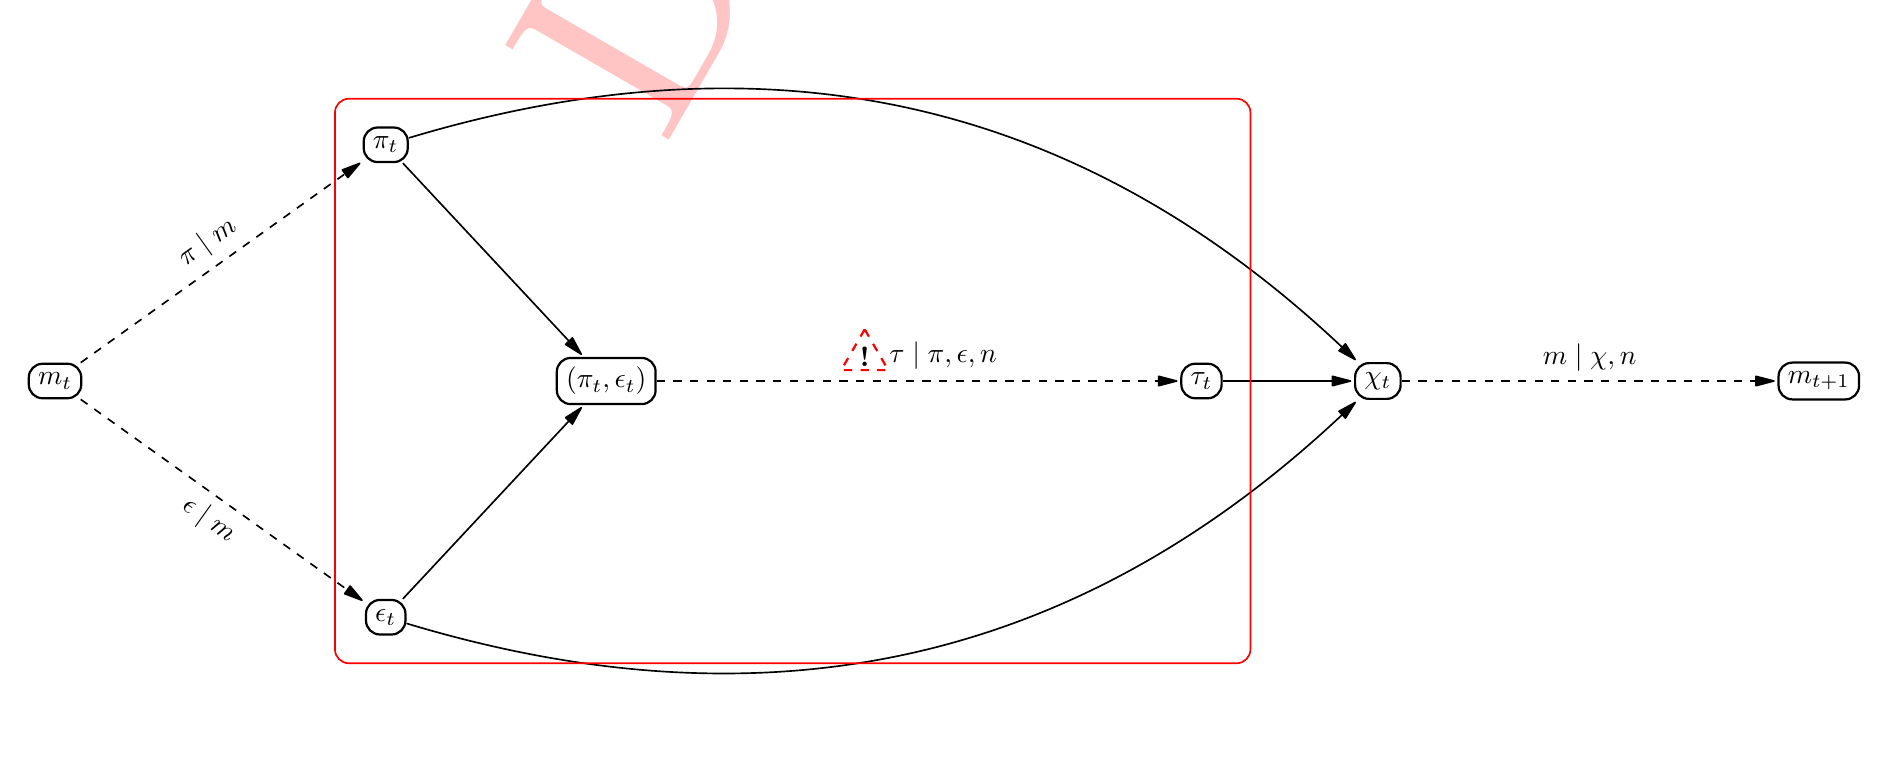
\begin{tikzpicture}[y=-3cm,x=2.8cm,
            > = {Stealth[inset=0pt,length=8pt,angle'=28,round]}, % arrow head style
            shorten > = 1pt, % don't touch arrow head to node
            auto,
%            node distance =1cm and 3cm, % distance between nodes
            semithick, % line style
            box/.style = {draw,red,inner sep=10pt,rounded corners=5pt}
        ]

        \tikzstyle{every state}=[
        rectangle,
        rounded corners=5pt,
            draw = black,
            thick,
            fill = white,
            minimum size = 4mm
        ]


        \node[state] at (0,1) (m) {$\countdetail_t$ };
        \node[state] at (1.5,0) (pi) {$\pi_t$ };
        \node[state] at (1.5,2) (epsilon) {$\epsilon_t$ };
        \node[state] at (2.5,1) (point) {$(\pi_t,\epsilon_t)$};
        \node[state] at (5.2,1) (tau) {$\tau_t$};
        \node[state] at (6,1) (chi) {$\chi_{t}$};
        \node[state] at (8,1) (mm) {$\countdetail_{t+1}$};
        
        \path[->,dashed] (m) edge node[above, sloped]  {$\pi\mid \countdetail$} (pi);
        \path[->,dashed] (m) edge node[below, sloped]  {$\epsilon\mid \countdetail$} (epsilon);
        \path[->] (pi) edge node {} (point);
        \path[->] (epsilon) edge node {} (point);
        \path[->,dashed] (point) edge node[above, sloped]  {\warningsign $\tau\mid \pi, \epsilon,n$} (tau);
        \path[->] (tau) edge node {} (chi);
        \path[->] (pi) edge [bend left] node {} (chi);
        \path[->] (epsilon) edge[bend right] node {} (chi);
        \path[->,dashed] (chi) edge node {$\countdetail\mid \chi,n$} (mm);
        \node[box,fit=(pi) (epsilon) (tau)]{};
    \end{tikzpicture}

\vspace{-1.5cm}}

}
%%%%%%%%%%%%%%%%%%%%%%%%%%%%%%%%%%%%%%%%%%%%%%%%%%%
\def\blockdiagnostic{
\block{Diagnostic}{
\begin{itemize}
\item When distributed according to the posterior law, the $\tau_{v,g,\indexvec{a}}$ are discrete and highly correlated. 
\item Sampling them independently does not work.
\end{itemize}
\vspace{-1cm}

    $$n_{.,s=1,.}=\begin{blockarray}{ccccc}
    &a=A&a=C&a=G&a=T&\\
    \begin{block}{c(cccc)}
 {\scriptscriptstyle v=1}&600&400&0&0\\   
 {\scriptscriptstyle v=2}&400&600&1&0\\
    \end{block}
\end{blockarray} $$

\vspace{-1.6cm}
$$\begin{blockarray}{ccc}
    &&\\&\scriptscriptstyle g=1&\scriptscriptstyle g=2\\
    \begin{block}{c(cc)}
 {\scriptscriptstyle v=1}&A&C\\   
  {\scriptscriptstyle v=2}&A&C\\   
    \end{block}
\end{blockarray} \overset{t=t+1}{\rightarrow}\begin{blockarray}{ccc}
    &&\\&\scriptscriptstyle g=1&\scriptscriptstyle g=2\\
    \begin{block}{c(cc)}
 {\scriptscriptstyle v=1}&A&C\\   
  {\scriptscriptstyle v=2}&C&C\\   
    \end{block}
\end{blockarray}\overset{t=t+1}{\rightarrow}\begin{blockarray}{ccc}
    &&\\&\scriptscriptstyle g=1&\scriptscriptstyle g=2\\
    \begin{block}{c(cc)}
 {\scriptscriptstyle v=1}&A&C\\   
  {\scriptscriptstyle v=2}&C&A\\   
    \end{block}
\end{blockarray}$$
}

	 \note[targetoffsety = -8cm,targetoffsetx = 2cm,rotate = 5]{\warningsign Sampler can't do this and stays stuck}
}
%%%%%%%%%%%%%%%%%%%%%%%%%%%%%%%%%%%%%%%%%%%%%%%%%%%
\def\blockrelax{\innerblock{Relaxation}{
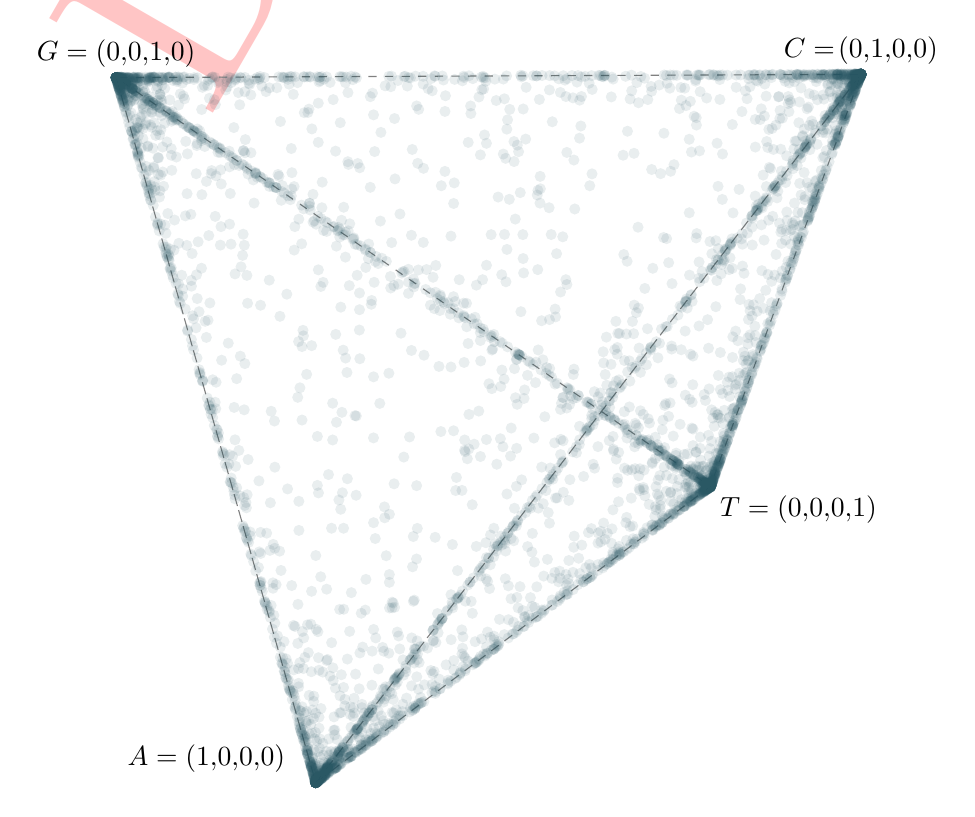
\begin{tikzpicture}[scale=10]


\begin{scope}[rotate around y=45,rotate around z=45]
 
% Draw the vertices of the tetrahedron

\coordinate (A) at (0, 0, 0);
\coordinate (C) at (1, 0, 0);
\coordinate (G) at (0.5, 0.866, 0);
\coordinate (T) at (0.5, 0.2887, 0.816);

%\foreach \p in {A,C,G,T}\fill[black] (\p) circle (0.02);

% Draw the edges of the cube
\draw[white!50!black, dashed]  (A) -- (C) -- (G) -- (A) -- (C) -- (T) -- (A) -- (T) -- (G) --  cycle;



    \pgfmathsetmacro{\alphaa}{0.1}       
       
\fill[color1,  opacity=\alphaa] (0.423,0.586,0.046) circle (.2pt);
         \fill[color1,  opacity=\alphaa] (0.984,0.027,0) circle (.2pt);
         \fill[color1,  opacity=\alphaa] (0.286,0.29,0.207) circle (.2pt);
         \fill[color1,  opacity=\alphaa] (0.842,0.106,0) circle (.2pt);
         \fill[color1,  opacity=\alphaa] (0.604,0.399,0.404) circle (.2pt);
         \fill[color1,  opacity=\alphaa] (0.093,0.02,0.057) circle (.2pt);
         \fill[color1,  opacity=\alphaa] (0,0,0) circle (.2pt);
         \fill[color1,  opacity=\alphaa] (0.231,0,0) circle (.2pt);
         \fill[color1,  opacity=\alphaa] (1,0,0) circle (.2pt);
         \fill[color1,  opacity=\alphaa] (0.36,0.556,0.003) circle (.2pt);
         \fill[color1,  opacity=\alphaa] (0.454,0.593,0.229) circle (.2pt);
         \fill[color1,  opacity=\alphaa] (0.506,0.85,0) circle (.2pt);
         \fill[color1,  opacity=\alphaa] (0.414,0.41,0.052) circle (.2pt);
         \fill[color1,  opacity=\alphaa] (0.533,0.269,0.762) circle (.2pt);
         \fill[color1,  opacity=\alphaa] (0.488,0.837,0) circle (.2pt);
         \fill[color1,  opacity=\alphaa] (0.001,0,0) circle (.2pt);
         \fill[color1,  opacity=\alphaa] (0.364,0.631,0) circle (.2pt);
         \fill[color1,  opacity=\alphaa] (0.495,0.836,0) circle (.2pt);
         \fill[color1,  opacity=\alphaa] (0.996,0.001,0) circle (.2pt);
         \fill[color1,  opacity=\alphaa] (0.999,0,0.001) circle (.2pt);
         \fill[color1,  opacity=\alphaa] (0.453,0.784,0) circle (.2pt);
         \fill[color1,  opacity=\alphaa] (0.405,0.235,0.66) circle (.2pt);
         \fill[color1,  opacity=\alphaa] (0.828,0.099,0.281) circle (.2pt);
         \fill[color1,  opacity=\alphaa] (0.648,0.186,0.526) circle (.2pt);
         \fill[color1,  opacity=\alphaa] (0.488,0.846,0) circle (.2pt);
         \fill[color1,  opacity=\alphaa] (0.47,0.438,0.499) circle (.2pt);
         \fill[color1,  opacity=\alphaa] (0.498,0.863,0) circle (.2pt);
         \fill[color1,  opacity=\alphaa] (0.006,0.01,0) circle (.2pt);
         \fill[color1,  opacity=\alphaa] (0.5,0.839,0.038) circle (.2pt);
         \fill[color1,  opacity=\alphaa] (0.605,0.051,0) circle (.2pt);
         \fill[color1,  opacity=\alphaa] (0.485,0.287,0.782) circle (.2pt);
         \fill[color1,  opacity=\alphaa] (0.516,0.502,0.418) circle (.2pt);
         \fill[color1,  opacity=\alphaa] (0.035,0.025,0.051) circle (.2pt);
         \fill[color1,  opacity=\alphaa] (0.5,0.289,0.816) circle (.2pt);
         \fill[color1,  opacity=\alphaa] (0.267,0.463,0) circle (.2pt);
         \fill[color1,  opacity=\alphaa] (0.5,0.289,0.816) circle (.2pt);
         \fill[color1,  opacity=\alphaa] (0.482,0.827,0) circle (.2pt);
         \fill[color1,  opacity=\alphaa] (0.5,0.298,0.804) circle (.2pt);
         \fill[color1,  opacity=\alphaa] (0.5,0.866,0) circle (.2pt);
         \fill[color1,  opacity=\alphaa] (0.5,0.289,0.816) circle (.2pt);
         \fill[color1,  opacity=\alphaa] (0.844,0.092,0.252) circle (.2pt);
         \fill[color1,  opacity=\alphaa] (0.476,0.583,0.341) circle (.2pt);
         \fill[color1,  opacity=\alphaa] (0.46,0.777,0.029) circle (.2pt);
         \fill[color1,  opacity=\alphaa] (0.996,0.007,0) circle (.2pt);
         \fill[color1,  opacity=\alphaa] (0.392,0.498,0.256) circle (.2pt);
         \fill[color1,  opacity=\alphaa] (0.977,0.013,0.038) circle (.2pt);
         \fill[color1,  opacity=\alphaa] (0.95,0.032,0.077) circle (.2pt);
         \fill[color1,  opacity=\alphaa] (0.436,0.611,0.002) circle (.2pt);
         \fill[color1,  opacity=\alphaa] (0.025,0.029,0.019) circle (.2pt);
         \fill[color1,  opacity=\alphaa] (0.952,0.028,0.079) circle (.2pt);
         \fill[color1,  opacity=\alphaa] (0.975,0.004,0.011) circle (.2pt);
         \fill[color1,  opacity=\alphaa] (0.006,0.002,0.006) circle (.2pt);
         \fill[color1,  opacity=\alphaa] (0.52,0.261,0.738) circle (.2pt);
         \fill[color1,  opacity=\alphaa] (0.319,0.184,0.521) circle (.2pt);
         \fill[color1,  opacity=\alphaa] (0.382,0.238,0.595) circle (.2pt);
         \fill[color1,  opacity=\alphaa] (0.207,0.357,0) circle (.2pt);
         \fill[color1,  opacity=\alphaa] (0.5,0.851,0.022) circle (.2pt);
         \fill[color1,  opacity=\alphaa] (0.575,0.22,0.616) circle (.2pt);
         \fill[color1,  opacity=\alphaa] (0.489,0.804,0.06) circle (.2pt);
         \fill[color1,  opacity=\alphaa] (0.968,0.006,0) circle (.2pt);
         \fill[color1,  opacity=\alphaa] (0.403,0,0) circle (.2pt);
         \fill[color1,  opacity=\alphaa] (0.008,0,0) circle (.2pt);
         \fill[color1,  opacity=\alphaa] (0.523,0.275,0.778) circle (.2pt);
         \fill[color1,  opacity=\alphaa] (0.5,0.474,0.554) circle (.2pt);
         \fill[color1,  opacity=\alphaa] (0.516,0.822,0.022) circle (.2pt);
         \fill[color1,  opacity=\alphaa] (0.021,0.001,0.003) circle (.2pt);
         \fill[color1,  opacity=\alphaa] (0.5,0.866,0) circle (.2pt);
         \fill[color1,  opacity=\alphaa] (0.339,0,0) circle (.2pt);
         \fill[color1,  opacity=\alphaa] (0.505,0.856,0.002) circle (.2pt);
         \fill[color1,  opacity=\alphaa] (0.002,0,0) circle (.2pt);
         \fill[color1,  opacity=\alphaa] (0.132,0.044,0.125) circle (.2pt);
         \fill[color1,  opacity=\alphaa] (0.508,0.851,0) circle (.2pt);
         \fill[color1,  opacity=\alphaa] (0,0,0) circle (.2pt);
         \fill[color1,  opacity=\alphaa] (0.831,0.29,0.003) circle (.2pt);
         \fill[color1,  opacity=\alphaa] (0,0,0) circle (.2pt);
         \fill[color1,  opacity=\alphaa] (0.502,0.301,0.793) circle (.2pt);
         \fill[color1,  opacity=\alphaa] (0.598,0.67,0.001) circle (.2pt);
         \fill[color1,  opacity=\alphaa] (0.5,0.846,0.028) circle (.2pt);
         \fill[color1,  opacity=\alphaa] (0.979,0.037,0) circle (.2pt);
         \fill[color1,  opacity=\alphaa] (0.548,0.78,0) circle (.2pt);
         \fill[color1,  opacity=\alphaa] (0.528,0.273,0.771) circle (.2pt);
         \fill[color1,  opacity=\alphaa] (0.445,0.769,0) circle (.2pt);
         \fill[color1,  opacity=\alphaa] (1,0,0) circle (.2pt);
         \fill[color1,  opacity=\alphaa] (0.461,0.264,0.748) circle (.2pt);
         \fill[color1,  opacity=\alphaa] (0.486,0.779,0.087) circle (.2pt);
         \fill[color1,  opacity=\alphaa] (0.074,0.018,0.034) circle (.2pt);
         \fill[color1,  opacity=\alphaa] (0.205,0.014,0.04) circle (.2pt);
         \fill[color1,  opacity=\alphaa] (0.501,0.288,0.815) circle (.2pt);
         \fill[color1,  opacity=\alphaa] (0.901,0.171,0) circle (.2pt);
         \fill[color1,  opacity=\alphaa] (0.5,0.305,0.793) circle (.2pt);
         \fill[color1,  opacity=\alphaa] (0.476,0.275,0.777) circle (.2pt);
         \fill[color1,  opacity=\alphaa] (0.563,0.749,0.011) circle (.2pt);
         \fill[color1,  opacity=\alphaa] (0.194,0.005,0.014) circle (.2pt);
         \fill[color1,  opacity=\alphaa] (0.5,0.289,0.816) circle (.2pt);
         \fill[color1,  opacity=\alphaa] (0.984,0,0) circle (.2pt);
         \fill[color1,  opacity=\alphaa] (0.97,0.016,0.013) circle (.2pt);
         \fill[color1,  opacity=\alphaa] (0.494,0.855,0) circle (.2pt);
         \fill[color1,  opacity=\alphaa] (0.497,0.287,0.811) circle (.2pt);
         \fill[color1,  opacity=\alphaa] (0.883,0.202,0) circle (.2pt);
         \fill[color1,  opacity=\alphaa] (0.305,0.055,0.001) circle (.2pt);
         \fill[color1,  opacity=\alphaa] (0.356,0.211,0.574) circle (.2pt);
         \fill[color1,  opacity=\alphaa] (0.02,0.035,0) circle (.2pt);
         \fill[color1,  opacity=\alphaa] (0.796,0.117,0.33) circle (.2pt);
         \fill[color1,  opacity=\alphaa] (0.391,0.161,0.43) circle (.2pt);
         \fill[color1,  opacity=\alphaa] (0.099,0.001,0) circle (.2pt);
         \fill[color1,  opacity=\alphaa] (0,0,0) circle (.2pt);
         \fill[color1,  opacity=\alphaa] (0.483,0.411,0.603) circle (.2pt);
         \fill[color1,  opacity=\alphaa] (0.5,0.289,0.816) circle (.2pt);
         \fill[color1,  opacity=\alphaa] (0.499,0.288,0.815) circle (.2pt);
         \fill[color1,  opacity=\alphaa] (0.499,0.864,0) circle (.2pt);
         \fill[color1,  opacity=\alphaa] (0.496,0.285,0.807) circle (.2pt);
         \fill[color1,  opacity=\alphaa] (0.493,0.852,0.002) circle (.2pt);
         \fill[color1,  opacity=\alphaa] (0.501,0.296,0.803) circle (.2pt);
         \fill[color1,  opacity=\alphaa] (0.155,0.26,0) circle (.2pt);
         \fill[color1,  opacity=\alphaa] (0.493,0.285,0.806) circle (.2pt);
         \fill[color1,  opacity=\alphaa] (0.581,0.14,0.377) circle (.2pt);
         \fill[color1,  opacity=\alphaa] (0.738,0,0) circle (.2pt);
         \fill[color1,  opacity=\alphaa] (0.655,0.199,0.563) circle (.2pt);
         \fill[color1,  opacity=\alphaa] (0.492,0.694,0.221) circle (.2pt);
         \fill[color1,  opacity=\alphaa] (0.502,0.86,0.004) circle (.2pt);
         \fill[color1,  opacity=\alphaa] (0.725,0.023,0.066) circle (.2pt);
         \fill[color1,  opacity=\alphaa] (0.029,0.049,0) circle (.2pt);
         \fill[color1,  opacity=\alphaa] (0.262,0,0) circle (.2pt);
         \fill[color1,  opacity=\alphaa] (0.382,0.368,0.414) circle (.2pt);
         \fill[color1,  opacity=\alphaa] (0.999,0.001,0.002) circle (.2pt);
         \fill[color1,  opacity=\alphaa] (0.5,0.313,0.783) circle (.2pt);
         \fill[color1,  opacity=\alphaa] (0.999,0,0) circle (.2pt);
         \fill[color1,  opacity=\alphaa] (0.496,0.858,0.001) circle (.2pt);
         \fill[color1,  opacity=\alphaa] (0.71,0.171,0.469) circle (.2pt);
         \fill[color1,  opacity=\alphaa] (0.025,0.014,0.041) circle (.2pt);
         \fill[color1,  opacity=\alphaa] (0.049,0,0) circle (.2pt);
         \fill[color1,  opacity=\alphaa] (0.439,0.15,0.424) circle (.2pt);
         \fill[color1,  opacity=\alphaa] (0.261,0.151,0.418) circle (.2pt);
         \fill[color1,  opacity=\alphaa] (0,0,0) circle (.2pt);
         \fill[color1,  opacity=\alphaa] (0.5,0.864,0.002) circle (.2pt);
         \fill[color1,  opacity=\alphaa] (0.347,0.427,0.242) circle (.2pt);
         \fill[color1,  opacity=\alphaa] (0.95,0.029,0.081) circle (.2pt);
         \fill[color1,  opacity=\alphaa] (1,0,0) circle (.2pt);
         \fill[color1,  opacity=\alphaa] (0.988,0.02,0) circle (.2pt);
         \fill[color1,  opacity=\alphaa] (0.784,0.124,0.35) circle (.2pt);
         \fill[color1,  opacity=\alphaa] (0.468,0.274,0.759) circle (.2pt);
         \fill[color1,  opacity=\alphaa] (0.286,0.093,0.263) circle (.2pt);
         \fill[color1,  opacity=\alphaa] (0.493,0.847,0.009) circle (.2pt);
         \fill[color1,  opacity=\alphaa] (0.927,0,0) circle (.2pt);
         \fill[color1,  opacity=\alphaa] (0.429,0,0) circle (.2pt);
         \fill[color1,  opacity=\alphaa] (0.916,0.047,0.133) circle (.2pt);
         \fill[color1,  opacity=\alphaa] (0.613,0,0.001) circle (.2pt);
         \fill[color1,  opacity=\alphaa] (0.5,0.327,0.763) circle (.2pt);
         \fill[color1,  opacity=\alphaa] (0.963,0.007,0) circle (.2pt);
         \fill[color1,  opacity=\alphaa] (0.534,0.268,0.759) circle (.2pt);
         \fill[color1,  opacity=\alphaa] (0.483,0.309,0.747) circle (.2pt);
         \fill[color1,  opacity=\alphaa] (0.499,0.865,0) circle (.2pt);
         \fill[color1,  opacity=\alphaa] (0.285,0.452,0.057) circle (.2pt);
         \fill[color1,  opacity=\alphaa] (0.848,0.088,0.247) circle (.2pt);
         \fill[color1,  opacity=\alphaa] (0.118,0.203,0.003) circle (.2pt);
         \fill[color1,  opacity=\alphaa] (1,0,0) circle (.2pt);
         \fill[color1,  opacity=\alphaa] (0.261,0.018,0.05) circle (.2pt);
         \fill[color1,  opacity=\alphaa] (0.5,0.866,0) circle (.2pt);
         \fill[color1,  opacity=\alphaa] (0.5,0.339,0.744) circle (.2pt);
         \fill[color1,  opacity=\alphaa] (0.066,0.113,0) circle (.2pt);
         \fill[color1,  opacity=\alphaa] (0.507,0.285,0.806) circle (.2pt);
         \fill[color1,  opacity=\alphaa] (0.023,0.004,0.01) circle (.2pt);
         \fill[color1,  opacity=\alphaa] (0.139,0.148,0) circle (.2pt);
         \fill[color1,  opacity=\alphaa] (0.507,0.332,0.74) circle (.2pt);
         \fill[color1,  opacity=\alphaa] (0.5,0.865,0.001) circle (.2pt);
         \fill[color1,  opacity=\alphaa] (0.5,0.301,0.799) circle (.2pt);
         \fill[color1,  opacity=\alphaa] (0.012,0.021,0) circle (.2pt);
         \fill[color1,  opacity=\alphaa] (0.459,0.767,0) circle (.2pt);
         \fill[color1,  opacity=\alphaa] (0.779,0.128,0.36) circle (.2pt);
         \fill[color1,  opacity=\alphaa] (0.5,0.699,0.236) circle (.2pt);
         \fill[color1,  opacity=\alphaa] (0.868,0.229,0) circle (.2pt);
         \fill[color1,  opacity=\alphaa] (0.004,0,0) circle (.2pt);
         \fill[color1,  opacity=\alphaa] (0.5,0.663,0.288) circle (.2pt);
         \fill[color1,  opacity=\alphaa] (0.496,0.507,0.498) circle (.2pt);
         \fill[color1,  opacity=\alphaa] (0.184,0.289,0.043) circle (.2pt);
         \fill[color1,  opacity=\alphaa] (0.5,0.863,0.004) circle (.2pt);
         \fill[color1,  opacity=\alphaa] (0.955,0.032,0.066) circle (.2pt);
         \fill[color1,  opacity=\alphaa] (0.484,0.838,0.002) circle (.2pt);
         \fill[color1,  opacity=\alphaa] (0.043,0.074,0) circle (.2pt);
         \fill[color1,  opacity=\alphaa] (0.501,0.31,0.784) circle (.2pt);
         \fill[color1,  opacity=\alphaa] (0.992,0.009,0) circle (.2pt);
         \fill[color1,  opacity=\alphaa] (0.491,0.851,0) circle (.2pt);
         \fill[color1,  opacity=\alphaa] (0.499,0.291,0.809) circle (.2pt);
         \fill[color1,  opacity=\alphaa] (0,0,0) circle (.2pt);
         \fill[color1,  opacity=\alphaa] (0.047,0.012,0.033) circle (.2pt);
         \fill[color1,  opacity=\alphaa] (0.961,0.067,0) circle (.2pt);
         \fill[color1,  opacity=\alphaa] (0.502,0.287,0.813) circle (.2pt);
         \fill[color1,  opacity=\alphaa] (0.499,0.288,0.814) circle (.2pt);
         \fill[color1,  opacity=\alphaa] (0.181,0.161,0) circle (.2pt);
         \fill[color1,  opacity=\alphaa] (0.455,0.783,0.001) circle (.2pt);
         \fill[color1,  opacity=\alphaa] (0.875,0,0) circle (.2pt);
         \fill[color1,  opacity=\alphaa] (0.505,0.304,0.782) circle (.2pt);
         \fill[color1,  opacity=\alphaa] (0.66,0.221,0.519) circle (.2pt);
         \fill[color1,  opacity=\alphaa] (0.564,0.252,0.712) circle (.2pt);
         \fill[color1,  opacity=\alphaa] (0.5,0.289,0.816) circle (.2pt);
         \fill[color1,  opacity=\alphaa] (0.5,0.289,0.816) circle (.2pt);
         \fill[color1,  opacity=\alphaa] (0.667,0.325,0.355) circle (.2pt);
         \fill[color1,  opacity=\alphaa] (1,0,0) circle (.2pt);
         \fill[color1,  opacity=\alphaa] (0.406,0.454,0.29) circle (.2pt);
         \fill[color1,  opacity=\alphaa] (0.55,0.776,0.004) circle (.2pt);
         \fill[color1,  opacity=\alphaa] (0.309,0.179,0.505) circle (.2pt);
         \fill[color1,  opacity=\alphaa] (0.5,0.861,0.007) circle (.2pt);
         \fill[color1,  opacity=\alphaa] (0.47,0.723,0.127) circle (.2pt);
         \fill[color1,  opacity=\alphaa] (0.061,0.03,0.083) circle (.2pt);
         \fill[color1,  opacity=\alphaa] (1,0,0) circle (.2pt);
         \fill[color1,  opacity=\alphaa] (0.5,0.288,0.816) circle (.2pt);
         \fill[color1,  opacity=\alphaa] (0.001,0,0) circle (.2pt);
         \fill[color1,  opacity=\alphaa] (0.5,0.865,0) circle (.2pt);
         \fill[color1,  opacity=\alphaa] (0.883,0.203,0) circle (.2pt);
         \fill[color1,  opacity=\alphaa] (0.224,0,0) circle (.2pt);
         \fill[color1,  opacity=\alphaa] (0.849,0.234,0) circle (.2pt);
         \fill[color1,  opacity=\alphaa] (0.484,0,0) circle (.2pt);
         \fill[color1,  opacity=\alphaa] (0.732,0.154,0.437) circle (.2pt);
         \fill[color1,  opacity=\alphaa] (0.998,0.001,0.004) circle (.2pt);
         \fill[color1,  opacity=\alphaa] (0.46,0.424,0.526) circle (.2pt);
         \fill[color1,  opacity=\alphaa] (0.524,0.825,0) circle (.2pt);
         \fill[color1,  opacity=\alphaa] (0.531,0.026,0.054) circle (.2pt);
         \fill[color1,  opacity=\alphaa] (0.022,0.001,0) circle (.2pt);
         \fill[color1,  opacity=\alphaa] (0.733,0.037,0.099) circle (.2pt);
         \fill[color1,  opacity=\alphaa] (0.5,0.339,0.745) circle (.2pt);
         \fill[color1,  opacity=\alphaa] (0.993,0.013,0) circle (.2pt);
         \fill[color1,  opacity=\alphaa] (0.5,0.857,0.013) circle (.2pt);
         \fill[color1,  opacity=\alphaa] (0.995,0.001,0.001) circle (.2pt);
         \fill[color1,  opacity=\alphaa] (0.075,0.103,0.039) circle (.2pt);
         \fill[color1,  opacity=\alphaa] (0.994,0.003,0.009) circle (.2pt);
         \fill[color1,  opacity=\alphaa] (0.855,0.021,0) circle (.2pt);
         \fill[color1,  opacity=\alphaa] (0.5,0.856,0.014) circle (.2pt);
         \fill[color1,  opacity=\alphaa] (0.995,0.003,0.008) circle (.2pt);
         \fill[color1,  opacity=\alphaa] (1,0,0) circle (.2pt);
         \fill[color1,  opacity=\alphaa] (0.002,0.001,0) circle (.2pt);
         \fill[color1,  opacity=\alphaa] (0.994,0,0.001) circle (.2pt);
         \fill[color1,  opacity=\alphaa] (0.493,0.281,0.794) circle (.2pt);
         \fill[color1,  opacity=\alphaa] (0.825,0.303,0) circle (.2pt);
         \fill[color1,  opacity=\alphaa] (0.501,0.859,0.008) circle (.2pt);
         \fill[color1,  opacity=\alphaa] (0.496,0.286,0.808) circle (.2pt);
         \fill[color1,  opacity=\alphaa] (0.497,0.283,0.799) circle (.2pt);
         \fill[color1,  opacity=\alphaa] (0.501,0.288,0.814) circle (.2pt);
         \fill[color1,  opacity=\alphaa] (0.502,0.298,0.798) circle (.2pt);
         \fill[color1,  opacity=\alphaa] (0.229,0.059,0.017) circle (.2pt);
         \fill[color1,  opacity=\alphaa] (0.5,0.858,0.011) circle (.2pt);
         \fill[color1,  opacity=\alphaa] (0.5,0.866,0) circle (.2pt);
         \fill[color1,  opacity=\alphaa] (0.17,0.06,0) circle (.2pt);
         \fill[color1,  opacity=\alphaa] (0.398,0.686,0.006) circle (.2pt);
         \fill[color1,  opacity=\alphaa] (0.949,0.071,0) circle (.2pt);
         \fill[color1,  opacity=\alphaa] (0.5,0.289,0.816) circle (.2pt);
         \fill[color1,  opacity=\alphaa] (0.976,0.03,0) circle (.2pt);
         \fill[color1,  opacity=\alphaa] (0.286,0.109,0.003) circle (.2pt);
         \fill[color1,  opacity=\alphaa] (0.002,0.001,0.002) circle (.2pt);
         \fill[color1,  opacity=\alphaa] (0.345,0.559,0) circle (.2pt);
         \fill[color1,  opacity=\alphaa] (0.456,0.633,0.219) circle (.2pt);
         \fill[color1,  opacity=\alphaa] (0.499,0.833,0.045) circle (.2pt);
         \fill[color1,  opacity=\alphaa] (0.01,0.005,0.002) circle (.2pt);
         \fill[color1,  opacity=\alphaa] (0.491,0.33,0.735) circle (.2pt);
         \fill[color1,  opacity=\alphaa] (0.554,0.752,0) circle (.2pt);
         \fill[color1,  opacity=\alphaa] (0.493,0.854,0) circle (.2pt);
         \fill[color1,  opacity=\alphaa] (0.999,0.001,0) circle (.2pt);
         \fill[color1,  opacity=\alphaa] (0.984,0.028,0) circle (.2pt);
         \fill[color1,  opacity=\alphaa] (0.999,0,0) circle (.2pt);
         \fill[color1,  opacity=\alphaa] (0.071,0.041,0.117) circle (.2pt);
         \fill[color1,  opacity=\alphaa] (0,0,0) circle (.2pt);
         \fill[color1,  opacity=\alphaa] (0.572,0.649,0.13) circle (.2pt);
         \fill[color1,  opacity=\alphaa] (0.406,0.235,0.662) circle (.2pt);
         \fill[color1,  opacity=\alphaa] (0.001,0.001,0.001) circle (.2pt);
         \fill[color1,  opacity=\alphaa] (0.998,0.001,0.003) circle (.2pt);
         \fill[color1,  opacity=\alphaa] (0.334,0,0) circle (.2pt);
         \fill[color1,  opacity=\alphaa] (0.989,0,0) circle (.2pt);
         \fill[color1,  opacity=\alphaa] (0.716,0.485,0.005) circle (.2pt);
         \fill[color1,  opacity=\alphaa] (0.002,0.004,0) circle (.2pt);
         \fill[color1,  opacity=\alphaa] (0.948,0.033,0.08) circle (.2pt);
         \fill[color1,  opacity=\alphaa] (0.996,0.002,0.007) circle (.2pt);
         \fill[color1,  opacity=\alphaa] (0.03,0.048,0) circle (.2pt);
         \fill[color1,  opacity=\alphaa] (0.503,0.335,0.744) circle (.2pt);
         \fill[color1,  opacity=\alphaa] (0.241,0.001,0) circle (.2pt);
         \fill[color1,  opacity=\alphaa] (0.063,0,0) circle (.2pt);
         \fill[color1,  opacity=\alphaa] (0.5,0.289,0.816) circle (.2pt);
         \fill[color1,  opacity=\alphaa] (0,0,0) circle (.2pt);
         \fill[color1,  opacity=\alphaa] (0.026,0,0) circle (.2pt);
         \fill[color1,  opacity=\alphaa] (0.021,0.037,0) circle (.2pt);
         \fill[color1,  opacity=\alphaa] (0.511,0.836,0.013) circle (.2pt);
         \fill[color1,  opacity=\alphaa] (0.953,0.027,0.076) circle (.2pt);
         \fill[color1,  opacity=\alphaa] (0.013,0,0) circle (.2pt);
         \fill[color1,  opacity=\alphaa] (0.452,0.288,0.7) circle (.2pt);
         \fill[color1,  opacity=\alphaa] (0.004,0.002,0.006) circle (.2pt);
         \fill[color1,  opacity=\alphaa] (0.455,0.055,0) circle (.2pt);
         \fill[color1,  opacity=\alphaa] (0.775,0.13,0.367) circle (.2pt);
         \fill[color1,  opacity=\alphaa] (0.5,0.289,0.816) circle (.2pt);
         \fill[color1,  opacity=\alphaa] (0.841,0,0) circle (.2pt);
         \fill[color1,  opacity=\alphaa] (0.732,0.004,0.009) circle (.2pt);
         \fill[color1,  opacity=\alphaa] (0.488,0.282,0.797) circle (.2pt);
         \fill[color1,  opacity=\alphaa] (0.003,0.005,0) circle (.2pt);
         \fill[color1,  opacity=\alphaa] (0.5,0.866,0.001) circle (.2pt);
         \fill[color1,  opacity=\alphaa] (0.513,0.281,0.796) circle (.2pt);
         \fill[color1,  opacity=\alphaa] (0.497,0.31,0.778) circle (.2pt);
         \fill[color1,  opacity=\alphaa] (0.83,0.289,0.007) circle (.2pt);
         \fill[color1,  opacity=\alphaa] (0.501,0.288,0.814) circle (.2pt);
         \fill[color1,  opacity=\alphaa] (0.5,0.29,0.815) circle (.2pt);
         \fill[color1,  opacity=\alphaa] (0.971,0.02,0.041) circle (.2pt);
         \fill[color1,  opacity=\alphaa] (0,0,0) circle (.2pt);
         \fill[color1,  opacity=\alphaa] (0.513,0.82,0.034) circle (.2pt);
         \fill[color1,  opacity=\alphaa] (0.518,0.67,0.234) circle (.2pt);
         \fill[color1,  opacity=\alphaa] (0.989,0.006,0.018) circle (.2pt);
         \fill[color1,  opacity=\alphaa] (1,0,0) circle (.2pt);
         \fill[color1,  opacity=\alphaa] (0.5,0.854,0.017) circle (.2pt);
         \fill[color1,  opacity=\alphaa] (0.501,0.797,0.059) circle (.2pt);
         \fill[color1,  opacity=\alphaa] (0.783,0.139,0.335) circle (.2pt);
         \fill[color1,  opacity=\alphaa] (0.194,0.135,0.01) circle (.2pt);
         \fill[color1,  opacity=\alphaa] (0.504,0.86,0) circle (.2pt);
         \fill[color1,  opacity=\alphaa] (0.915,0.049,0.139) circle (.2pt);
         \fill[color1,  opacity=\alphaa] (0.006,0.003,0.01) circle (.2pt);
         \fill[color1,  opacity=\alphaa] (0.5,0.393,0.669) circle (.2pt);
         \fill[color1,  opacity=\alphaa] (0.001,0,0.001) circle (.2pt);
         \fill[color1,  opacity=\alphaa] (0.916,0.089,0.065) circle (.2pt);
         \fill[color1,  opacity=\alphaa] (0.003,0,0) circle (.2pt);
         \fill[color1,  opacity=\alphaa] (0.552,0.216,0.612) circle (.2pt);
         \fill[color1,  opacity=\alphaa] (0.987,0.023,0) circle (.2pt);
         \fill[color1,  opacity=\alphaa] (0.883,0,0) circle (.2pt);
         \fill[color1,  opacity=\alphaa] (0.362,0,0) circle (.2pt);
         \fill[color1,  opacity=\alphaa] (0.952,0.003,0.003) circle (.2pt);
         \fill[color1,  opacity=\alphaa] (0.091,0.151,0.009) circle (.2pt);
         \fill[color1,  opacity=\alphaa] (0.426,0.733,0.007) circle (.2pt);
         \fill[color1,  opacity=\alphaa] (0.5,0.861,0.007) circle (.2pt);
         \fill[color1,  opacity=\alphaa] (0.5,0.289,0.816) circle (.2pt);
         \fill[color1,  opacity=\alphaa] (0.62,0.658,0) circle (.2pt);
         \fill[color1,  opacity=\alphaa] (0.785,0.341,0.044) circle (.2pt);
         \fill[color1,  opacity=\alphaa] (0.004,0.007,0) circle (.2pt);
         \fill[color1,  opacity=\alphaa] (0.702,0.185,0.416) circle (.2pt);
         \fill[color1,  opacity=\alphaa] (0.071,0.041,0.116) circle (.2pt);
         \fill[color1,  opacity=\alphaa] (0.498,0.311,0.781) circle (.2pt);
         \fill[color1,  opacity=\alphaa] (0.499,0.86,0.006) circle (.2pt);
         \fill[color1,  opacity=\alphaa] (0.508,0.85,0) circle (.2pt);
         \fill[color1,  opacity=\alphaa] (0.006,0,0) circle (.2pt);
         \fill[color1,  opacity=\alphaa] (0.523,0.826,0) circle (.2pt);
         \fill[color1,  opacity=\alphaa] (0.001,0,0) circle (.2pt);
         \fill[color1,  opacity=\alphaa] (0.49,0.087,0.243) circle (.2pt);
         \fill[color1,  opacity=\alphaa] (0.5,0.857,0.013) circle (.2pt);
         \fill[color1,  opacity=\alphaa] (0.5,0.771,0.134) circle (.2pt);
         \fill[color1,  opacity=\alphaa] (0.444,0.365,0.572) circle (.2pt);
         \fill[color1,  opacity=\alphaa] (0.313,0.175,0.494) circle (.2pt);
         \fill[color1,  opacity=\alphaa] (0.497,0.287,0.812) circle (.2pt);
         \fill[color1,  opacity=\alphaa] (0.167,0.096,0.273) circle (.2pt);
         \fill[color1,  opacity=\alphaa] (0.5,0.528,0.477) circle (.2pt);
         \fill[color1,  opacity=\alphaa] (0.473,0.791,0.039) circle (.2pt);
         \fill[color1,  opacity=\alphaa] (0.892,0.187,0) circle (.2pt);
         \fill[color1,  opacity=\alphaa] (0.187,0.003,0) circle (.2pt);
         \fill[color1,  opacity=\alphaa] (0.497,0.857,0) circle (.2pt);
         \fill[color1,  opacity=\alphaa] (1,0,0) circle (.2pt);
         \fill[color1,  opacity=\alphaa] (0.031,0.018,0.051) circle (.2pt);
         \fill[color1,  opacity=\alphaa] (0.495,0.857,0) circle (.2pt);
         \fill[color1,  opacity=\alphaa] (0.807,0.3,0) circle (.2pt);
         \fill[color1,  opacity=\alphaa] (0.226,0.131,0.37) circle (.2pt);
         \fill[color1,  opacity=\alphaa] (0.984,0,0) circle (.2pt);
         \fill[color1,  opacity=\alphaa] (0.498,0.288,0.813) circle (.2pt);
         \fill[color1,  opacity=\alphaa] (0.011,0.019,0) circle (.2pt);
         \fill[color1,  opacity=\alphaa] (0.5,0.289,0.816) circle (.2pt);
         \fill[color1,  opacity=\alphaa] (0.936,0.11,0) circle (.2pt);
         \fill[color1,  opacity=\alphaa] (0.491,0.283,0.801) circle (.2pt);
         \fill[color1,  opacity=\alphaa] (0.419,0.242,0.675) circle (.2pt);
         \fill[color1,  opacity=\alphaa] (0.538,0.267,0.754) circle (.2pt);
         \fill[color1,  opacity=\alphaa] (0.501,0.288,0.814) circle (.2pt);
         \fill[color1,  opacity=\alphaa] (0.5,0.355,0.722) circle (.2pt);
         \fill[color1,  opacity=\alphaa] (0,0.001,0) circle (.2pt);
         \fill[color1,  opacity=\alphaa] (0.286,0.165,0.467) circle (.2pt);
         \fill[color1,  opacity=\alphaa] (0.5,0.67,0.277) circle (.2pt);
         \fill[color1,  opacity=\alphaa] (0.03,0,0) circle (.2pt);
         \fill[color1,  opacity=\alphaa] (0.072,0.035,0.099) circle (.2pt);
         \fill[color1,  opacity=\alphaa] (0.491,0.283,0.8) circle (.2pt);
         \fill[color1,  opacity=\alphaa] (0.113,0.146,0) circle (.2pt);
         \fill[color1,  opacity=\alphaa] (0.5,0.445,0.594) circle (.2pt);
         \fill[color1,  opacity=\alphaa] (0.246,0.426,0) circle (.2pt);
         \fill[color1,  opacity=\alphaa] (0.528,0.219,0.618) circle (.2pt);
         \fill[color1,  opacity=\alphaa] (0.985,0.012,0.021) circle (.2pt);
         \fill[color1,  opacity=\alphaa] (0.503,0.291,0.803) circle (.2pt);
         \fill[color1,  opacity=\alphaa] (0.5,0.85,0.023) circle (.2pt);
         \fill[color1,  opacity=\alphaa] (0.201,0.339,0.012) circle (.2pt);
         \fill[color1,  opacity=\alphaa] (0.5,0.766,0.141) circle (.2pt);
         \fill[color1,  opacity=\alphaa] (0.069,0.075,0.063) circle (.2pt);
         \fill[color1,  opacity=\alphaa] (0.999,0,0.001) circle (.2pt);
         \fill[color1,  opacity=\alphaa] (0.722,0.161,0.454) circle (.2pt);
         \fill[color1,  opacity=\alphaa] (0.501,0.3,0.798) circle (.2pt);
         \fill[color1,  opacity=\alphaa] (0.264,0.153,0.432) circle (.2pt);
         \fill[color1,  opacity=\alphaa] (0.077,0,0) circle (.2pt);
         \fill[color1,  opacity=\alphaa] (0.812,0.088,0.239) circle (.2pt);
         \fill[color1,  opacity=\alphaa] (0.565,0.488,0.376) circle (.2pt);
         \fill[color1,  opacity=\alphaa] (0.968,0.055,0) circle (.2pt);
         \fill[color1,  opacity=\alphaa] (0,0,0.001) circle (.2pt);
         \fill[color1,  opacity=\alphaa] (0.526,0.822,0) circle (.2pt);
         \fill[color1,  opacity=\alphaa] (0.467,0.27,0.762) circle (.2pt);
         \fill[color1,  opacity=\alphaa] (0.025,0,0) circle (.2pt);
         \fill[color1,  opacity=\alphaa] (0.5,0.325,0.765) circle (.2pt);
         \fill[color1,  opacity=\alphaa] (0.257,0.301,0.143) circle (.2pt);
         \fill[color1,  opacity=\alphaa] (0.009,0,0.001) circle (.2pt);
         \fill[color1,  opacity=\alphaa] (0.686,0.53,0.019) circle (.2pt);
         \fill[color1,  opacity=\alphaa] (0.5,0.866,0) circle (.2pt);
         \fill[color1,  opacity=\alphaa] (0.735,0.191,0.38) circle (.2pt);
         \fill[color1,  opacity=\alphaa] (0.499,0.864,0) circle (.2pt);
         \fill[color1,  opacity=\alphaa] (0,0,0) circle (.2pt);
         \fill[color1,  opacity=\alphaa] (0.971,0.051,0) circle (.2pt);
         \fill[color1,  opacity=\alphaa] (0.934,0.047,0) circle (.2pt);
         \fill[color1,  opacity=\alphaa] (0.5,0.501,0.517) circle (.2pt);
         \fill[color1,  opacity=\alphaa] (0.125,0.189,0.037) circle (.2pt);
         \fill[color1,  opacity=\alphaa] (0.5,0.861,0.006) circle (.2pt);
         \fill[color1,  opacity=\alphaa] (0.5,0.788,0.109) circle (.2pt);
         \fill[color1,  opacity=\alphaa] (0.003,0.003,0.002) circle (.2pt);
         \fill[color1,  opacity=\alphaa] (0.501,0.865,0) circle (.2pt);
         \fill[color1,  opacity=\alphaa] (0.931,0.072,0.012) circle (.2pt);
         \fill[color1,  opacity=\alphaa] (0.5,0.865,0) circle (.2pt);
         \fill[color1,  opacity=\alphaa] (1,0.001,0) circle (.2pt);
         \fill[color1,  opacity=\alphaa] (0.004,0.007,0) circle (.2pt);
         \fill[color1,  opacity=\alphaa] (0.237,0.395,0) circle (.2pt);
         \fill[color1,  opacity=\alphaa] (0.499,0.294,0.807) circle (.2pt);
         \fill[color1,  opacity=\alphaa] (0.516,0.28,0.791) circle (.2pt);
         \fill[color1,  opacity=\alphaa] (0.461,0.172,0.486) circle (.2pt);
         \fill[color1,  opacity=\alphaa] (0.454,0.262,0.741) circle (.2pt);
         \fill[color1,  opacity=\alphaa] (0.013,0,0) circle (.2pt);
         \fill[color1,  opacity=\alphaa] (0.409,0.238,0.665) circle (.2pt);
         \fill[color1,  opacity=\alphaa] (0.5,0.866,0) circle (.2pt);
         \fill[color1,  opacity=\alphaa] (0.485,0.363,0.674) circle (.2pt);
         \fill[color1,  opacity=\alphaa] (0.489,0.417,0.608) circle (.2pt);
         \fill[color1,  opacity=\alphaa] (1,0,0) circle (.2pt);
         \fill[color1,  opacity=\alphaa] (0.001,0.001,0) circle (.2pt);
         \fill[color1,  opacity=\alphaa] (0.497,0.287,0.812) circle (.2pt);
         \fill[color1,  opacity=\alphaa] (0.037,0.005,0.014) circle (.2pt);
         \fill[color1,  opacity=\alphaa] (0.85,0.084,0.237) circle (.2pt);
         \fill[color1,  opacity=\alphaa] (0.46,0.537,0.286) circle (.2pt);
         \fill[color1,  opacity=\alphaa] (0.5,0.289,0.816) circle (.2pt);
         \fill[color1,  opacity=\alphaa] (0.5,0.289,0.816) circle (.2pt);
         \fill[color1,  opacity=\alphaa] (0.488,0.843,0.003) circle (.2pt);
         \fill[color1,  opacity=\alphaa] (0.482,0.278,0.783) circle (.2pt);
         \fill[color1,  opacity=\alphaa] (0.54,0.318,0.677) circle (.2pt);
         \fill[color1,  opacity=\alphaa] (0.5,0.289,0.816) circle (.2pt);
         \fill[color1,  opacity=\alphaa] (0.491,0.808,0) circle (.2pt);
         \fill[color1,  opacity=\alphaa] (0.727,0,0) circle (.2pt);
         \fill[color1,  opacity=\alphaa] (0,0,0) circle (.2pt);
         \fill[color1,  opacity=\alphaa] (0.699,0.174,0.491) circle (.2pt);
         \fill[color1,  opacity=\alphaa] (0,0,0) circle (.2pt);
         \fill[color1,  opacity=\alphaa] (0.5,0.865,0.001) circle (.2pt);
         \fill[color1,  opacity=\alphaa] (0.996,0.006,0.001) circle (.2pt);
         \fill[color1,  opacity=\alphaa] (0.901,0.172,0) circle (.2pt);
         \fill[color1,  opacity=\alphaa] (0.466,0.64,0.236) circle (.2pt);
         \fill[color1,  opacity=\alphaa] (0.062,0.034,0.094) circle (.2pt);
         \fill[color1,  opacity=\alphaa] (0.986,0.023,0) circle (.2pt);
         \fill[color1,  opacity=\alphaa] (0.997,0.002,0.005) circle (.2pt);
         \fill[color1,  opacity=\alphaa] (0.499,0.288,0.814) circle (.2pt);
         \fill[color1,  opacity=\alphaa] (0.963,0,0) circle (.2pt);
         \fill[color1,  opacity=\alphaa] (0,0,0) circle (.2pt);
         \fill[color1,  opacity=\alphaa] (0.354,0.339,0.387) circle (.2pt);
         \fill[color1,  opacity=\alphaa] (0.471,0.372,0.628) circle (.2pt);
         \fill[color1,  opacity=\alphaa] (0.971,0.017,0.046) circle (.2pt);
         \fill[color1,  opacity=\alphaa] (0.49,0.281,0.795) circle (.2pt);
         \fill[color1,  opacity=\alphaa] (0.583,0.722,0.001) circle (.2pt);
         \fill[color1,  opacity=\alphaa] (0.487,0.844,0) circle (.2pt);
         \fill[color1,  opacity=\alphaa] (0.129,0.217,0.01) circle (.2pt);
         \fill[color1,  opacity=\alphaa] (0.998,0,0) circle (.2pt);
         \fill[color1,  opacity=\alphaa] (0.504,0.86,0) circle (.2pt);
         \fill[color1,  opacity=\alphaa] (0,0,0) circle (.2pt);
         \fill[color1,  opacity=\alphaa] (0.5,0.289,0.816) circle (.2pt);
         \fill[color1,  opacity=\alphaa] (0.896,0.002,0.005) circle (.2pt);
         \fill[color1,  opacity=\alphaa] (0.961,0.066,0.002) circle (.2pt);
         \fill[color1,  opacity=\alphaa] (0.554,0.313,0.651) circle (.2pt);
         \fill[color1,  opacity=\alphaa] (0.502,0.861,0) circle (.2pt);
         \fill[color1,  opacity=\alphaa] (0.587,0.278,0.609) circle (.2pt);
         \fill[color1,  opacity=\alphaa] (0.487,0.819,0.033) circle (.2pt);
         \fill[color1,  opacity=\alphaa] (0.457,0.791,0) circle (.2pt);
         \fill[color1,  opacity=\alphaa] (0.5,0.425,0.623) circle (.2pt);
         \fill[color1,  opacity=\alphaa] (0.426,0.235,0.663) circle (.2pt);
         \fill[color1,  opacity=\alphaa] (0.511,0,0) circle (.2pt);
         \fill[color1,  opacity=\alphaa] (0.023,0,0) circle (.2pt);
         \fill[color1,  opacity=\alphaa] (0.518,0.829,0.009) circle (.2pt);
         \fill[color1,  opacity=\alphaa] (0.877,0.002,0) circle (.2pt);
         \fill[color1,  opacity=\alphaa] (0.604,0.228,0.646) circle (.2pt);
         \fill[color1,  opacity=\alphaa] (0.027,0.042,0) circle (.2pt);
         \fill[color1,  opacity=\alphaa] (0.976,0.039,0) circle (.2pt);
         \fill[color1,  opacity=\alphaa] (0.497,0.291,0.806) circle (.2pt);
         \fill[color1,  opacity=\alphaa] (0.496,0.571,0.406) circle (.2pt);
         \fill[color1,  opacity=\alphaa] (0.558,0.371,0.385) circle (.2pt);
         \fill[color1,  opacity=\alphaa] (0.5,0.35,0.729) circle (.2pt);
         \fill[color1,  opacity=\alphaa] (0.268,0.265,0) circle (.2pt);
         \fill[color1,  opacity=\alphaa] (0.015,0.025,0) circle (.2pt);
         \fill[color1,  opacity=\alphaa] (0.487,0.449,0.558) circle (.2pt);
         \fill[color1,  opacity=\alphaa] (1,0,0) circle (.2pt);
         \fill[color1,  opacity=\alphaa] (0.989,0.006,0.017) circle (.2pt);
         \fill[color1,  opacity=\alphaa] (0.442,0.489,0.391) circle (.2pt);
         \fill[color1,  opacity=\alphaa] (0.508,0.85,0.003) circle (.2pt);
         \fill[color1,  opacity=\alphaa] (0.124,0.024,0.067) circle (.2pt);
         \fill[color1,  opacity=\alphaa] (0.121,0,0) circle (.2pt);
         \fill[color1,  opacity=\alphaa] (0.501,0.289,0.815) circle (.2pt);
         \fill[color1,  opacity=\alphaa] (0.496,0.778,0.115) circle (.2pt);
         \fill[color1,  opacity=\alphaa] (0,0,0) circle (.2pt);
         \fill[color1,  opacity=\alphaa] (0.047,0.064,0) circle (.2pt);
         \fill[color1,  opacity=\alphaa] (0.919,0.14,0) circle (.2pt);
         \fill[color1,  opacity=\alphaa] (0.925,0.129,0) circle (.2pt);
         \fill[color1,  opacity=\alphaa] (0.536,0.805,0) circle (.2pt);
         \fill[color1,  opacity=\alphaa] (0.996,0,0) circle (.2pt);
         \fill[color1,  opacity=\alphaa] (0.517,0.391,0.63) circle (.2pt);
         \fill[color1,  opacity=\alphaa] (0.459,0.267,0.747) circle (.2pt);
         \fill[color1,  opacity=\alphaa] (0.673,0.124,0.352) circle (.2pt);
         \fill[color1,  opacity=\alphaa] (0.036,0.062,0) circle (.2pt);
         \fill[color1,  opacity=\alphaa] (0.5,0.289,0.816) circle (.2pt);
         \fill[color1,  opacity=\alphaa] (0.184,0.103,0.293) circle (.2pt);
         \fill[color1,  opacity=\alphaa] (0.508,0.298,0.785) circle (.2pt);
         \fill[color1,  opacity=\alphaa] (0.5,0.289,0.816) circle (.2pt);
         \fill[color1,  opacity=\alphaa] (0.5,0.866,0) circle (.2pt);
         \fill[color1,  opacity=\alphaa] (0.732,0.412,0.057) circle (.2pt);
         \fill[color1,  opacity=\alphaa] (0.953,0.018,0.05) circle (.2pt);
         \fill[color1,  opacity=\alphaa] (0.467,0.776,0.045) circle (.2pt);
         \fill[color1,  opacity=\alphaa] (0.281,0.306,0.255) circle (.2pt);
         \fill[color1,  opacity=\alphaa] (0.905,0.134,0) circle (.2pt);
         \fill[color1,  opacity=\alphaa] (0,0,0) circle (.2pt);
         \fill[color1,  opacity=\alphaa] (0.974,0.044,0.001) circle (.2pt);
         \fill[color1,  opacity=\alphaa] (0.5,0.427,0.621) circle (.2pt);
         \fill[color1,  opacity=\alphaa] (0.577,0.517,0) circle (.2pt);
         \fill[color1,  opacity=\alphaa] (0.491,0.587,0.371) circle (.2pt);
         \fill[color1,  opacity=\alphaa] (0.737,0.456,0) circle (.2pt);
         \fill[color1,  opacity=\alphaa] (0.5,0.289,0.816) circle (.2pt);
         \fill[color1,  opacity=\alphaa] (0.96,0.066,0) circle (.2pt);
         \fill[color1,  opacity=\alphaa] (0.901,0,0) circle (.2pt);
         \fill[color1,  opacity=\alphaa] (0.5,0.862,0.006) circle (.2pt);
         \fill[color1,  opacity=\alphaa] (0.023,0.039,0) circle (.2pt);
         \fill[color1,  opacity=\alphaa] (0.081,0.075,0.091) circle (.2pt);
         \fill[color1,  opacity=\alphaa] (0.719,0.162,0.458) circle (.2pt);
         \fill[color1,  opacity=\alphaa] (0.5,0.289,0.816) circle (.2pt);
         \fill[color1,  opacity=\alphaa] (0.034,0.059,0) circle (.2pt);
         \fill[color1,  opacity=\alphaa] (0.753,0.143,0.404) circle (.2pt);
         \fill[color1,  opacity=\alphaa] (0.483,0.837,0) circle (.2pt);
         \fill[color1,  opacity=\alphaa] (0.042,0.049,0) circle (.2pt);
         \fill[color1,  opacity=\alphaa] (0.968,0.054,0.001) circle (.2pt);
         \fill[color1,  opacity=\alphaa] (0.153,0.084,0.236) circle (.2pt);
         \fill[color1,  opacity=\alphaa] (1,0,0) circle (.2pt);
         \fill[color1,  opacity=\alphaa] (0.499,0.289,0.815) circle (.2pt);
         \fill[color1,  opacity=\alphaa] (0.002,0.002,0) circle (.2pt);
         \fill[color1,  opacity=\alphaa] (0.5,0.289,0.816) circle (.2pt);
         \fill[color1,  opacity=\alphaa] (0.5,0.619,0.349) circle (.2pt);
         \fill[color1,  opacity=\alphaa] (0.499,0.811,0.077) circle (.2pt);
         \fill[color1,  opacity=\alphaa] (1,0,0) circle (.2pt);
         \fill[color1,  opacity=\alphaa] (0.109,0.104,0.119) circle (.2pt);
         \fill[color1,  opacity=\alphaa] (0.484,0.838,0) circle (.2pt);
         \fill[color1,  opacity=\alphaa] (0.216,0.124,0) circle (.2pt);
         \fill[color1,  opacity=\alphaa] (0.017,0,0) circle (.2pt);
         \fill[color1,  opacity=\alphaa] (0.919,0.003,0) circle (.2pt);
         \fill[color1,  opacity=\alphaa] (0.637,0.625,0.005) circle (.2pt);
         \fill[color1,  opacity=\alphaa] (0.5,0.837,0.041) circle (.2pt);
         \fill[color1,  opacity=\alphaa] (0.524,0.819,0.009) circle (.2pt);
         \fill[color1,  opacity=\alphaa] (1,0,0) circle (.2pt);
         \fill[color1,  opacity=\alphaa] (0.96,0.031,0.053) circle (.2pt);
         \fill[color1,  opacity=\alphaa] (0.109,0.189,0.001) circle (.2pt);
         \fill[color1,  opacity=\alphaa] (0.818,0.209,0.151) circle (.2pt);
         \fill[color1,  opacity=\alphaa] (0.021,0.015,0.031) circle (.2pt);
         \fill[color1,  opacity=\alphaa] (0.5,0.796,0.099) circle (.2pt);
         \fill[color1,  opacity=\alphaa] (0.319,0.244,0.435) circle (.2pt);
         \fill[color1,  opacity=\alphaa] (0.843,0,0) circle (.2pt);
         \fill[color1,  opacity=\alphaa] (0.501,0.288,0.815) circle (.2pt);
         \fill[color1,  opacity=\alphaa] (0.973,0.016,0.045) circle (.2pt);
         \fill[color1,  opacity=\alphaa] (0.796,0.197,0.221) circle (.2pt);
         \fill[color1,  opacity=\alphaa] (0.502,0.862,0) circle (.2pt);
         \fill[color1,  opacity=\alphaa] (0.02,0.012,0.033) circle (.2pt);
         \fill[color1,  opacity=\alphaa] (0.175,0.018,0.052) circle (.2pt);
         \fill[color1,  opacity=\alphaa] (0.495,0.856,0) circle (.2pt);
         \fill[color1,  opacity=\alphaa] (0.992,0.004,0.012) circle (.2pt);
         \fill[color1,  opacity=\alphaa] (0.502,0.862,0) circle (.2pt);
         \fill[color1,  opacity=\alphaa] (0.261,0,0) circle (.2pt);
         \fill[color1,  opacity=\alphaa] (0.953,0.081,0) circle (.2pt);
         \fill[color1,  opacity=\alphaa] (0.929,0.123,0) circle (.2pt);
         \fill[color1,  opacity=\alphaa] (0.568,0.266,0.679) circle (.2pt);
         \fill[color1,  opacity=\alphaa] (0.976,0.014,0.039) circle (.2pt);
         \fill[color1,  opacity=\alphaa] (0.514,0.288,0.783) circle (.2pt);
         \fill[color1,  opacity=\alphaa] (0.5,0.289,0.816) circle (.2pt);
         \fill[color1,  opacity=\alphaa] (0.897,0.046,0.13) circle (.2pt);
         \fill[color1,  opacity=\alphaa] (0.508,0.284,0.803) circle (.2pt);
         \fill[color1,  opacity=\alphaa] (0.501,0.864,0) circle (.2pt);
         \fill[color1,  opacity=\alphaa] (0.5,0.866,0) circle (.2pt);
         \fill[color1,  opacity=\alphaa] (0.622,0.452,0.044) circle (.2pt);
         \fill[color1,  opacity=\alphaa] (0.501,0.73,0.189) circle (.2pt);
         \fill[color1,  opacity=\alphaa] (0.39,0.314,0.326) circle (.2pt);
         \fill[color1,  opacity=\alphaa] (0.512,0.841,0) circle (.2pt);
         \fill[color1,  opacity=\alphaa] (0.388,0.425,0.047) circle (.2pt);
         \fill[color1,  opacity=\alphaa] (0.637,0.21,0.593) circle (.2pt);
         \fill[color1,  opacity=\alphaa] (0.727,0.21,0.367) circle (.2pt);
         \fill[color1,  opacity=\alphaa] (0.51,0.845,0) circle (.2pt);
         \fill[color1,  opacity=\alphaa] (0.5,0.866,0) circle (.2pt);
         \fill[color1,  opacity=\alphaa] (0.86,0.081,0.229) circle (.2pt);
         \fill[color1,  opacity=\alphaa] (0.5,0.324,0.766) circle (.2pt);
         \fill[color1,  opacity=\alphaa] (0.31,0.536,0) circle (.2pt);
         \fill[color1,  opacity=\alphaa] (0.608,0.333,0.487) circle (.2pt);
         \fill[color1,  opacity=\alphaa] (0.228,0,0) circle (.2pt);
         \fill[color1,  opacity=\alphaa] (0.498,0.857,0.007) circle (.2pt);
         \fill[color1,  opacity=\alphaa] (0.515,0.568,0.384) circle (.2pt);
         \fill[color1,  opacity=\alphaa] (0.542,0.764,0.043) circle (.2pt);
         \fill[color1,  opacity=\alphaa] (0.504,0.83,0.034) circle (.2pt);
         \fill[color1,  opacity=\alphaa] (0.011,0.01,0.012) circle (.2pt);
         \fill[color1,  opacity=\alphaa] (0.002,0.001,0.003) circle (.2pt);
         \fill[color1,  opacity=\alphaa] (0.898,0,0) circle (.2pt);
         \fill[color1,  opacity=\alphaa] (0.114,0.109,0) circle (.2pt);
         \fill[color1,  opacity=\alphaa] (0.603,0.646,0.003) circle (.2pt);
         \fill[color1,  opacity=\alphaa] (0.498,0.681,0.256) circle (.2pt);
         \fill[color1,  opacity=\alphaa] (0.499,0.864,0) circle (.2pt);
         \fill[color1,  opacity=\alphaa] (0.172,0.297,0) circle (.2pt);
         \fill[color1,  opacity=\alphaa] (0.995,0,0) circle (.2pt);
         \fill[color1,  opacity=\alphaa] (0.4,0.032,0) circle (.2pt);
         \fill[color1,  opacity=\alphaa] (0.853,0.106,0.187) circle (.2pt);
         \fill[color1,  opacity=\alphaa] (0.5,0.289,0.816) circle (.2pt);
         \fill[color1,  opacity=\alphaa] (0.616,0.657,0.012) circle (.2pt);
         \fill[color1,  opacity=\alphaa] (0.997,0.002,0.002) circle (.2pt);
         \fill[color1,  opacity=\alphaa] (0.011,0.003,0) circle (.2pt);
         \fill[color1,  opacity=\alphaa] (0.728,0.461,0.003) circle (.2pt);
         \fill[color1,  opacity=\alphaa] (0.994,0.011,0) circle (.2pt);
         \fill[color1,  opacity=\alphaa] (0.543,0.265,0.745) circle (.2pt);
         \fill[color1,  opacity=\alphaa] (0.448,0.47,0.43) circle (.2pt);
         \fill[color1,  opacity=\alphaa] (0.996,0.002,0.007) circle (.2pt);
         \fill[color1,  opacity=\alphaa] (0.895,0.046,0.129) circle (.2pt);
         \fill[color1,  opacity=\alphaa] (0.475,0.274,0.776) circle (.2pt);
         \fill[color1,  opacity=\alphaa] (0.503,0.858,0) circle (.2pt);
         \fill[color1,  opacity=\alphaa] (0.5,0.289,0.816) circle (.2pt);
         \fill[color1,  opacity=\alphaa] (1,0,0) circle (.2pt);
         \fill[color1,  opacity=\alphaa] (0.5,0.865,0) circle (.2pt);
         \fill[color1,  opacity=\alphaa] (0.34,0.551,0.013) circle (.2pt);
         \fill[color1,  opacity=\alphaa] (0.104,0.053,0) circle (.2pt);
         \fill[color1,  opacity=\alphaa] (0.39,0.225,0.637) circle (.2pt);
         \fill[color1,  opacity=\alphaa] (0.413,0.185,0.36) circle (.2pt);
         \fill[color1,  opacity=\alphaa] (0.931,0.042,0.072) circle (.2pt);
         \fill[color1,  opacity=\alphaa] (0.5,0.289,0.816) circle (.2pt);
         \fill[color1,  opacity=\alphaa] (0.999,0,0.001) circle (.2pt);
         \fill[color1,  opacity=\alphaa] (0.001,0,0) circle (.2pt);
         \fill[color1,  opacity=\alphaa] (0.498,0.854,0.011) circle (.2pt);
         \fill[color1,  opacity=\alphaa] (0.797,0.119,0.329) circle (.2pt);
         \fill[color1,  opacity=\alphaa] (0.607,0.458,0.314) circle (.2pt);
         \fill[color1,  opacity=\alphaa] (0.512,0.394,0.637) circle (.2pt);
         \fill[color1,  opacity=\alphaa] (0.981,0.033,0) circle (.2pt);
         \fill[color1,  opacity=\alphaa] (0.5,0.624,0.343) circle (.2pt);
         \fill[color1,  opacity=\alphaa] (0.484,0.102,0) circle (.2pt);
         \fill[color1,  opacity=\alphaa] (0.498,0.863,0) circle (.2pt);
         \fill[color1,  opacity=\alphaa] (0.5,0.866,0) circle (.2pt);
         \fill[color1,  opacity=\alphaa] (0.492,0.284,0.802) circle (.2pt);
         \fill[color1,  opacity=\alphaa] (0.381,0.22,0.621) circle (.2pt);
         \fill[color1,  opacity=\alphaa] (0.408,0.317,0.424) circle (.2pt);
         \fill[color1,  opacity=\alphaa] (1,0.001,0) circle (.2pt);
         \fill[color1,  opacity=\alphaa] (0.226,0.004,0.007) circle (.2pt);
         \fill[color1,  opacity=\alphaa] (0.269,0.453,0.001) circle (.2pt);
         \fill[color1,  opacity=\alphaa] (0.499,0.288,0.816) circle (.2pt);
         \fill[color1,  opacity=\alphaa] (0.025,0.003,0.002) circle (.2pt);
         \fill[color1,  opacity=\alphaa] (1,0,0) circle (.2pt);
         \fill[color1,  opacity=\alphaa] (0.29,0.203,0.424) circle (.2pt);
         \fill[color1,  opacity=\alphaa] (0.525,0.27,0.001) circle (.2pt);
         \fill[color1,  opacity=\alphaa] (0.5,0.289,0.816) circle (.2pt);
         \fill[color1,  opacity=\alphaa] (0.009,0.006,0.014) circle (.2pt);
         \fill[color1,  opacity=\alphaa] (0.5,0.866,0) circle (.2pt);
         \fill[color1,  opacity=\alphaa] (0.153,0,0) circle (.2pt);
         \fill[color1,  opacity=\alphaa] (0.5,0.865,0) circle (.2pt);
         \fill[color1,  opacity=\alphaa] (0.029,0.013,0.038) circle (.2pt);
         \fill[color1,  opacity=\alphaa] (0.808,0,0) circle (.2pt);
         \fill[color1,  opacity=\alphaa] (0.214,0.123,0.349) circle (.2pt);
         \fill[color1,  opacity=\alphaa] (0.228,0.049,0) circle (.2pt);
         \fill[color1,  opacity=\alphaa] (0.979,0,0) circle (.2pt);
         \fill[color1,  opacity=\alphaa] (0.057,0.033,0.094) circle (.2pt);
         \fill[color1,  opacity=\alphaa] (0.376,0.217,0.613) circle (.2pt);
         \fill[color1,  opacity=\alphaa] (0.951,0.083,0) circle (.2pt);
         \fill[color1,  opacity=\alphaa] (0.182,0.196,0.167) circle (.2pt);
         \fill[color1,  opacity=\alphaa] (0.443,0.768,0) circle (.2pt);
         \fill[color1,  opacity=\alphaa] (0.452,0.784,0) circle (.2pt);
         \fill[color1,  opacity=\alphaa] (0.019,0,0) circle (.2pt);
         \fill[color1,  opacity=\alphaa] (0.668,0.464,0.156) circle (.2pt);
         \fill[color1,  opacity=\alphaa] (0.5,0.289,0.815) circle (.2pt);
         \fill[color1,  opacity=\alphaa] (0.029,0.028,0.004) circle (.2pt);
         \fill[color1,  opacity=\alphaa] (0.287,0.164,0.436) circle (.2pt);
         \fill[color1,  opacity=\alphaa] (0.525,0.818,0.007) circle (.2pt);
         \fill[color1,  opacity=\alphaa] (0.259,0,0) circle (.2pt);
         \fill[color1,  opacity=\alphaa] (0.033,0.021,0.052) circle (.2pt);
         \fill[color1,  opacity=\alphaa] (0.761,0.381,0.048) circle (.2pt);
         \fill[color1,  opacity=\alphaa] (0.5,0.474,0.554) circle (.2pt);
         \fill[color1,  opacity=\alphaa] (0.631,0.197,0.557) circle (.2pt);
         \fill[color1,  opacity=\alphaa] (0.58,0.247,0.678) circle (.2pt);
         \fill[color1,  opacity=\alphaa] (0.337,0.228,0.503) circle (.2pt);
         \fill[color1,  opacity=\alphaa] (0.999,0.001,0.001) circle (.2pt);
         \fill[color1,  opacity=\alphaa] (0.394,0.253,0.608) circle (.2pt);
         \fill[color1,  opacity=\alphaa] (0.93,0.04,0.114) circle (.2pt);
         \fill[color1,  opacity=\alphaa] (0.512,0.839,0) circle (.2pt);
         \fill[color1,  opacity=\alphaa] (0,0,0) circle (.2pt);
         \fill[color1,  opacity=\alphaa] (0.497,0.287,0.812) circle (.2pt);
         \fill[color1,  opacity=\alphaa] (0.99,0.006,0.017) circle (.2pt);
         \fill[color1,  opacity=\alphaa] (0.501,0.865,0) circle (.2pt);
         \fill[color1,  opacity=\alphaa] (1,0,0) circle (.2pt);
         \fill[color1,  opacity=\alphaa] (0.512,0.846,0) circle (.2pt);
         \fill[color1,  opacity=\alphaa] (0.216,0.125,0.352) circle (.2pt);
         \fill[color1,  opacity=\alphaa] (0.662,0.083,0.039) circle (.2pt);
         \fill[color1,  opacity=\alphaa] (0.799,0.112,0.315) circle (.2pt);
         \fill[color1,  opacity=\alphaa] (0.061,0.082,0.033) circle (.2pt);
         \fill[color1,  opacity=\alphaa] (0.506,0.287,0.803) circle (.2pt);
         \fill[color1,  opacity=\alphaa] (0.5,0.861,0.007) circle (.2pt);
         \fill[color1,  opacity=\alphaa] (0.635,0.632,0) circle (.2pt);
         \fill[color1,  opacity=\alphaa] (0.5,0.292,0.812) circle (.2pt);
         \fill[color1,  opacity=\alphaa] (0.5,0.289,0.816) circle (.2pt);
         \fill[color1,  opacity=\alphaa] (0.003,0.004,0.001) circle (.2pt);
         \fill[color1,  opacity=\alphaa] (0.373,0.201,0) circle (.2pt);
         \fill[color1,  opacity=\alphaa] (0.5,0.862,0.006) circle (.2pt);
         \fill[color1,  opacity=\alphaa] (0.038,0.012,0.032) circle (.2pt);
         \fill[color1,  opacity=\alphaa] (0.239,0.21,0) circle (.2pt);
         \fill[color1,  opacity=\alphaa] (0.501,0.857,0.005) circle (.2pt);
         \fill[color1,  opacity=\alphaa] (0.507,0.262,0.741) circle (.2pt);
         \fill[color1,  opacity=\alphaa] (0.006,0,0) circle (.2pt);
         \fill[color1,  opacity=\alphaa] (0.5,0.866,0) circle (.2pt);
         \fill[color1,  opacity=\alphaa] (0,0,0) circle (.2pt);
         \fill[color1,  opacity=\alphaa] (0.5,0.294,0.809) circle (.2pt);
         \fill[color1,  opacity=\alphaa] (0.714,0.495,0) circle (.2pt);
         \fill[color1,  opacity=\alphaa] (0.891,0.005,0.001) circle (.2pt);
         \fill[color1,  opacity=\alphaa] (1,0,0) circle (.2pt);
         \fill[color1,  opacity=\alphaa] (0.999,0,0.001) circle (.2pt);
         \fill[color1,  opacity=\alphaa] (1,0,0) circle (.2pt);
         \fill[color1,  opacity=\alphaa] (0.013,0.009,0.019) circle (.2pt);
         \fill[color1,  opacity=\alphaa] (0.611,0.673,0) circle (.2pt);
         \fill[color1,  opacity=\alphaa] (0.017,0.03,0) circle (.2pt);
         \fill[color1,  opacity=\alphaa] (0.492,0.109,0) circle (.2pt);
         \fill[color1,  opacity=\alphaa] (0.997,0.002,0.005) circle (.2pt);
         \fill[color1,  opacity=\alphaa] (0.487,0.281,0.794) circle (.2pt);
         \fill[color1,  opacity=\alphaa] (0.001,0.001,0) circle (.2pt);
         \fill[color1,  opacity=\alphaa] (0.38,0.658,0) circle (.2pt);
         \fill[color1,  opacity=\alphaa] (0.5,0.866,0) circle (.2pt);
         \fill[color1,  opacity=\alphaa] (0.5,0.289,0.816) circle (.2pt);
         \fill[color1,  opacity=\alphaa] (0.037,0.006,0.013) circle (.2pt);
         \fill[color1,  opacity=\alphaa] (0.464,0.178,0.503) circle (.2pt);
         \fill[color1,  opacity=\alphaa] (0.467,0.711,0.139) circle (.2pt);
         \fill[color1,  opacity=\alphaa] (0.335,0.001,0) circle (.2pt);
         \fill[color1,  opacity=\alphaa] (0.729,0.191,0.394) circle (.2pt);
         \fill[color1,  opacity=\alphaa] (0.258,0.088,0.012) circle (.2pt);
         \fill[color1,  opacity=\alphaa] (0.997,0.001,0.004) circle (.2pt);
         \fill[color1,  opacity=\alphaa] (0.538,0.793,0) circle (.2pt);
         \fill[color1,  opacity=\alphaa] (0.605,0.239,0.621) circle (.2pt);
         \fill[color1,  opacity=\alphaa] (0.884,0.008,0.022) circle (.2pt);
         \fill[color1,  opacity=\alphaa] (0.024,0.01,0.029) circle (.2pt);
         \fill[color1,  opacity=\alphaa] (0.996,0.008,0) circle (.2pt);
         \fill[color1,  opacity=\alphaa] (0.5,0.289,0.816) circle (.2pt);
         \fill[color1,  opacity=\alphaa] (0.975,0.043,0) circle (.2pt);
         \fill[color1,  opacity=\alphaa] (0.999,0.001,0) circle (.2pt);
         \fill[color1,  opacity=\alphaa] (0.499,0.288,0.815) circle (.2pt);
         \fill[color1,  opacity=\alphaa] (0.514,0.257,0.71) circle (.2pt);
         \fill[color1,  opacity=\alphaa] (0.139,0.075,0.204) circle (.2pt);
         \fill[color1,  opacity=\alphaa] (0.5,0.717,0.211) circle (.2pt);
         \fill[color1,  opacity=\alphaa] (0.999,0,0) circle (.2pt);
         \fill[color1,  opacity=\alphaa] (0.501,0.848,0) circle (.2pt);
         \fill[color1,  opacity=\alphaa] (0.5,0.297,0.805) circle (.2pt);
         \fill[color1,  opacity=\alphaa] (0.023,0.013,0.037) circle (.2pt);
         \fill[color1,  opacity=\alphaa] (0.831,0.019,0.054) circle (.2pt);
         \fill[color1,  opacity=\alphaa] (0.899,0.176,0) circle (.2pt);
         \fill[color1,  opacity=\alphaa] (0.925,0.043,0.122) circle (.2pt);
         \fill[color1,  opacity=\alphaa] (1,0,0) circle (.2pt);
         \fill[color1,  opacity=\alphaa] (1,0,0) circle (.2pt);
         \fill[color1,  opacity=\alphaa] (0.5,0.864,0.002) circle (.2pt);
         \fill[color1,  opacity=\alphaa] (0.473,0.696,0.175) circle (.2pt);
         \fill[color1,  opacity=\alphaa] (0.771,0.13,0.367) circle (.2pt);
         \fill[color1,  opacity=\alphaa] (0,0,0) circle (.2pt);
         \fill[color1,  opacity=\alphaa] (0.5,0.289,0.816) circle (.2pt);
         \fill[color1,  opacity=\alphaa] (0.5,0.858,0.01) circle (.2pt);
         \fill[color1,  opacity=\alphaa] (0.5,0.866,0) circle (.2pt);
         \fill[color1,  opacity=\alphaa] (0.5,0.866,0) circle (.2pt);
         \fill[color1,  opacity=\alphaa] (0.5,0.655,0.298) circle (.2pt);
         \fill[color1,  opacity=\alphaa] (0.694,0.53,0) circle (.2pt);
         \fill[color1,  opacity=\alphaa] (0.51,0.281,0.796) circle (.2pt);
         \fill[color1,  opacity=\alphaa] (0.929,0.067,0.011) circle (.2pt);
         \fill[color1,  opacity=\alphaa] (0.939,0,0) circle (.2pt);
         \fill[color1,  opacity=\alphaa] (0.001,0.001,0.001) circle (.2pt);
         \fill[color1,  opacity=\alphaa] (0.595,0.698,0) circle (.2pt);
         \fill[color1,  opacity=\alphaa] (0.244,0.422,0) circle (.2pt);
         \fill[color1,  opacity=\alphaa] (0.5,0.289,0.816) circle (.2pt);
         \fill[color1,  opacity=\alphaa] (0,0,0) circle (.2pt);
         \fill[color1,  opacity=\alphaa] (0.789,0.305,0) circle (.2pt);
         \fill[color1,  opacity=\alphaa] (0.997,0.001,0.004) circle (.2pt);
         \fill[color1,  opacity=\alphaa] (0.495,0.273,0.771) circle (.2pt);
         \fill[color1,  opacity=\alphaa] (0.506,0.856,0) circle (.2pt);
         \fill[color1,  opacity=\alphaa] (0.115,0.071,0.183) circle (.2pt);
         \fill[color1,  opacity=\alphaa] (0.756,0.141,0.398) circle (.2pt);
         \fill[color1,  opacity=\alphaa] (0.586,0.709,0) circle (.2pt);
         \fill[color1,  opacity=\alphaa] (0.998,0,0) circle (.2pt);
         \fill[color1,  opacity=\alphaa] (0.998,0.001,0.004) circle (.2pt);
         \fill[color1,  opacity=\alphaa] (0.062,0.087,0.03) circle (.2pt);
         \fill[color1,  opacity=\alphaa] (0.055,0.076,0) circle (.2pt);
         \fill[color1,  opacity=\alphaa] (0.5,0.86,0.008) circle (.2pt);
         \fill[color1,  opacity=\alphaa] (0.44,0.261,0.705) circle (.2pt);
         \fill[color1,  opacity=\alphaa] (0.041,0.051,0.027) circle (.2pt);
         \fill[color1,  opacity=\alphaa] (0.498,0.631,0.327) circle (.2pt);
         \fill[color1,  opacity=\alphaa] (0.516,0.279,0.79) circle (.2pt);
         \fill[color1,  opacity=\alphaa] (0.602,0.226,0.583) circle (.2pt);
         \fill[color1,  opacity=\alphaa] (0.5,0.739,0.179) circle (.2pt);
         \fill[color1,  opacity=\alphaa] (0.522,0.826,0) circle (.2pt);
         \fill[color1,  opacity=\alphaa] (0.479,0.804,0.035) circle (.2pt);
         \fill[color1,  opacity=\alphaa] (0.505,0.857,0) circle (.2pt);
         \fill[color1,  opacity=\alphaa] (0.953,0.027,0.075) circle (.2pt);
         \fill[color1,  opacity=\alphaa] (0.507,0.853,0.001) circle (.2pt);
         \fill[color1,  opacity=\alphaa] (0.8,0.339,0) circle (.2pt);
         \fill[color1,  opacity=\alphaa] (0.5,0.85,0.022) circle (.2pt);
         \fill[color1,  opacity=\alphaa] (0.434,0.713,0) circle (.2pt);
         \fill[color1,  opacity=\alphaa] (0.996,0,0) circle (.2pt);
         \fill[color1,  opacity=\alphaa] (0.89,0.191,0.001) circle (.2pt);
         \fill[color1,  opacity=\alphaa] (0.847,0.001,0.002) circle (.2pt);
         \fill[color1,  opacity=\alphaa] (0.49,0.284,0.797) circle (.2pt);
         \fill[color1,  opacity=\alphaa] (0.393,0.674,0.01) circle (.2pt);
         \fill[color1,  opacity=\alphaa] (0.205,0.333,0) circle (.2pt);
         \fill[color1,  opacity=\alphaa] (0.724,0.436,0.018) circle (.2pt);
         \fill[color1,  opacity=\alphaa] (1,0,0) circle (.2pt);
         \fill[color1,  opacity=\alphaa] (0.497,0.285,0.805) circle (.2pt);
         \fill[color1,  opacity=\alphaa] (0.5,0.289,0.816) circle (.2pt);
         \fill[color1,  opacity=\alphaa] (0.263,0.152,0.429) circle (.2pt);
         \fill[color1,  opacity=\alphaa] (0.204,0.353,0) circle (.2pt);
         \fill[color1,  opacity=\alphaa] (0.63,0.641,0) circle (.2pt);
         \fill[color1,  opacity=\alphaa] (0.684,0.427,0.17) circle (.2pt);
         \fill[color1,  opacity=\alphaa] (0.496,0.818,0.058) circle (.2pt);
         \fill[color1,  opacity=\alphaa] (0.001,0,0) circle (.2pt);
         \fill[color1,  opacity=\alphaa] (0.5,0.864,0.002) circle (.2pt);
         \fill[color1,  opacity=\alphaa] (0.998,0,0) circle (.2pt);
         \fill[color1,  opacity=\alphaa] (0.924,0.047,0.119) circle (.2pt);
         \fill[color1,  opacity=\alphaa] (0.552,0.775,0) circle (.2pt);
         \fill[color1,  opacity=\alphaa] (0.843,0.254,0) circle (.2pt);
         \fill[color1,  opacity=\alphaa] (0.136,0.234,0) circle (.2pt);
         \fill[color1,  opacity=\alphaa] (0.436,0.252,0.712) circle (.2pt);
         \fill[color1,  opacity=\alphaa] (0.5,0.866,0) circle (.2pt);
         \fill[color1,  opacity=\alphaa] (0.751,0.144,0.407) circle (.2pt);
         \fill[color1,  opacity=\alphaa] (0.236,0.107,0.304) circle (.2pt);
         \fill[color1,  opacity=\alphaa] (1,0,0) circle (.2pt);
         \fill[color1,  opacity=\alphaa] (0.047,0.006,0.017) circle (.2pt);
         \fill[color1,  opacity=\alphaa] (0.131,0.073,0.207) circle (.2pt);
         \fill[color1,  opacity=\alphaa] (0.495,0.418,0.622) circle (.2pt);
         \fill[color1,  opacity=\alphaa] (0.512,0.844,0.002) circle (.2pt);
         \fill[color1,  opacity=\alphaa] (0.497,0.861,0) circle (.2pt);
         \fill[color1,  opacity=\alphaa] (0.515,0.368,0.667) circle (.2pt);
         \fill[color1,  opacity=\alphaa] (0.448,0.056,0.158) circle (.2pt);
         \fill[color1,  opacity=\alphaa] (0.495,0.857,0) circle (.2pt);
         \fill[color1,  opacity=\alphaa] (1,0,0) circle (.2pt);
         \fill[color1,  opacity=\alphaa] (0.5,0.866,0) circle (.2pt);
         \fill[color1,  opacity=\alphaa] (0.584,0.507,0) circle (.2pt);
         \fill[color1,  opacity=\alphaa] (0.984,0.028,0) circle (.2pt);
         \fill[color1,  opacity=\alphaa] (0.6,0.208,0.283) circle (.2pt);
         \fill[color1,  opacity=\alphaa] (0.25,0,0) circle (.2pt);
         \fill[color1,  opacity=\alphaa] (0.5,0.334,0.753) circle (.2pt);
         \fill[color1,  opacity=\alphaa] (0.484,0.28,0.791) circle (.2pt);
         \fill[color1,  opacity=\alphaa] (0.572,0.261,0.68) circle (.2pt);
         \fill[color1,  opacity=\alphaa] (0.843,0.091,0.255) circle (.2pt);
         \fill[color1,  opacity=\alphaa] (0.533,0.271,0.761) circle (.2pt);
         \fill[color1,  opacity=\alphaa] (0.5,0.855,0.015) circle (.2pt);
         \fill[color1,  opacity=\alphaa] (0.5,0.865,0.001) circle (.2pt);
         \fill[color1,  opacity=\alphaa] (0.427,0.73,0.012) circle (.2pt);
         \fill[color1,  opacity=\alphaa] (0.003,0.005,0.001) circle (.2pt);
         \fill[color1,  opacity=\alphaa] (0.5,0.289,0.816) circle (.2pt);
         \fill[color1,  opacity=\alphaa] (1,0,0) circle (.2pt);
         \fill[color1,  opacity=\alphaa] (0.5,0.289,0.815) circle (.2pt);
         \fill[color1,  opacity=\alphaa] (0.015,0.001,0.004) circle (.2pt);
         \fill[color1,  opacity=\alphaa] (0.846,0.267,0) circle (.2pt);
         \fill[color1,  opacity=\alphaa] (0.232,0,0) circle (.2pt);
         \fill[color1,  opacity=\alphaa] (0.972,0.016,0.045) circle (.2pt);
         \fill[color1,  opacity=\alphaa] (0.541,0.265,0.75) circle (.2pt);
         \fill[color1,  opacity=\alphaa] (0.5,0.864,0.003) circle (.2pt);
         \fill[color1,  opacity=\alphaa] (0.938,0.001,0.002) circle (.2pt);
         \fill[color1,  opacity=\alphaa] (0.506,0.703,0.216) circle (.2pt);
         \fill[color1,  opacity=\alphaa] (0.028,0.039,0.012) circle (.2pt);
         \fill[color1,  opacity=\alphaa] (0.641,0.621,0) circle (.2pt);
         \fill[color1,  opacity=\alphaa] (0.063,0.036,0.103) circle (.2pt);
         \fill[color1,  opacity=\alphaa] (0.358,0.62,0.001) circle (.2pt);
         \fill[color1,  opacity=\alphaa] (0.048,0.016,0.046) circle (.2pt);
         \fill[color1,  opacity=\alphaa] (0.002,0.001,0.004) circle (.2pt);
         \fill[color1,  opacity=\alphaa] (0.492,0.661,0.27) circle (.2pt);
         \fill[color1,  opacity=\alphaa] (0.394,0.227,0.643) circle (.2pt);
         \fill[color1,  opacity=\alphaa] (0.491,0.85,0) circle (.2pt);
         \fill[color1,  opacity=\alphaa] (0.891,0.007,0.015) circle (.2pt);
         \fill[color1,  opacity=\alphaa] (0.084,0.144,0) circle (.2pt);
         \fill[color1,  opacity=\alphaa] (0.005,0,0) circle (.2pt);
         \fill[color1,  opacity=\alphaa] (0.497,0.861,0) circle (.2pt);
         \fill[color1,  opacity=\alphaa] (1,0,0) circle (.2pt);
         \fill[color1,  opacity=\alphaa] (0.994,0.008,0.004) circle (.2pt);
         \fill[color1,  opacity=\alphaa] (0.502,0.851,0.002) circle (.2pt);
         \fill[color1,  opacity=\alphaa] (0.732,0.445,0.028) circle (.2pt);
         \fill[color1,  opacity=\alphaa] (0.053,0.091,0) circle (.2pt);
         \fill[color1,  opacity=\alphaa] (0.488,0.582,0.21) circle (.2pt);
         \fill[color1,  opacity=\alphaa] (0.766,0.023,0.063) circle (.2pt);
         \fill[color1,  opacity=\alphaa] (0.213,0.369,0) circle (.2pt);
         \fill[color1,  opacity=\alphaa] (0.5,0.298,0.804) circle (.2pt);
         \fill[color1,  opacity=\alphaa] (0.049,0.003,0.008) circle (.2pt);
         \fill[color1,  opacity=\alphaa] (0.594,0.061,0) circle (.2pt);
         \fill[color1,  opacity=\alphaa] (0.011,0.019,0) circle (.2pt);
         \fill[color1,  opacity=\alphaa] (0.5,0.866,0) circle (.2pt);
         \fill[color1,  opacity=\alphaa] (0.916,0.047,0.132) circle (.2pt);
         \fill[color1,  opacity=\alphaa] (0.5,0.32,0.772) circle (.2pt);
         \fill[color1,  opacity=\alphaa] (0,0,0) circle (.2pt);
         \fill[color1,  opacity=\alphaa] (0.99,0.01,0) circle (.2pt);
         \fill[color1,  opacity=\alphaa] (0.332,0.201,0.528) circle (.2pt);
         \fill[color1,  opacity=\alphaa] (0.5,0.865,0) circle (.2pt);
         \fill[color1,  opacity=\alphaa] (0.588,0,0) circle (.2pt);
         \fill[color1,  opacity=\alphaa] (0.493,0.515,0.476) circle (.2pt);
         \fill[color1,  opacity=\alphaa] (0.646,0.553,0.082) circle (.2pt);
         \fill[color1,  opacity=\alphaa] (0.514,0.304,0.742) circle (.2pt);
         \fill[color1,  opacity=\alphaa] (0.519,0.827,0) circle (.2pt);
         \fill[color1,  opacity=\alphaa] (0.499,0.289,0.814) circle (.2pt);
         \fill[color1,  opacity=\alphaa] (0.506,0.854,0.001) circle (.2pt);
         \fill[color1,  opacity=\alphaa] (0.434,0.07,0.007) circle (.2pt);
         \fill[color1,  opacity=\alphaa] (0.5,0.289,0.816) circle (.2pt);
         \fill[color1,  opacity=\alphaa] (1,0,0) circle (.2pt);
         \fill[color1,  opacity=\alphaa] (0.507,0.32,0.754) circle (.2pt);
         \fill[color1,  opacity=\alphaa] (0.505,0.855,0) circle (.2pt);
         \fill[color1,  opacity=\alphaa] (0.5,0.289,0.816) circle (.2pt);
         \fill[color1,  opacity=\alphaa] (0.997,0,0) circle (.2pt);
         \fill[color1,  opacity=\alphaa] (0.837,0.142,0.2) circle (.2pt);
         \fill[color1,  opacity=\alphaa] (0.999,0,0) circle (.2pt);
         \fill[color1,  opacity=\alphaa] (0.997,0.001,0.004) circle (.2pt);
         \fill[color1,  opacity=\alphaa] (0,0,0) circle (.2pt);
         \fill[color1,  opacity=\alphaa] (0.808,0.002,0.005) circle (.2pt);
         \fill[color1,  opacity=\alphaa] (0.498,0.303,0.792) circle (.2pt);
         \fill[color1,  opacity=\alphaa] (0.923,0.093,0.058) circle (.2pt);
         \fill[color1,  opacity=\alphaa] (0.066,0.04,0.105) circle (.2pt);
         \fill[color1,  opacity=\alphaa] (1,0,0) circle (.2pt);
         \fill[color1,  opacity=\alphaa] (0.434,0.247,0.699) circle (.2pt);
         \fill[color1,  opacity=\alphaa] (0.585,0,0) circle (.2pt);
         \fill[color1,  opacity=\alphaa] (0.5,0.288,0.815) circle (.2pt);
         \fill[color1,  opacity=\alphaa] (0.076,0.044,0.125) circle (.2pt);
         \fill[color1,  opacity=\alphaa] (0.993,0.01,0.002) circle (.2pt);
         \fill[color1,  opacity=\alphaa] (0.5,0.289,0.816) circle (.2pt);
         \fill[color1,  opacity=\alphaa] (0.456,0.23,0) circle (.2pt);
         \fill[color1,  opacity=\alphaa] (0.79,0.104,0.295) circle (.2pt);
         \fill[color1,  opacity=\alphaa] (0.026,0.015,0.043) circle (.2pt);
         \fill[color1,  opacity=\alphaa] (0.839,0,0.001) circle (.2pt);
         \fill[color1,  opacity=\alphaa] (0.485,0.056,0.141) circle (.2pt);
         \fill[color1,  opacity=\alphaa] (0.037,0.032,0.037) circle (.2pt);
         \fill[color1,  opacity=\alphaa] (0.711,0.165,0.466) circle (.2pt);
         \fill[color1,  opacity=\alphaa] (0.258,0.249,0.28) circle (.2pt);
         \fill[color1,  opacity=\alphaa] (0,0,0) circle (.2pt);
         \fill[color1,  opacity=\alphaa] (0.924,0.124,0.012) circle (.2pt);
         \fill[color1,  opacity=\alphaa] (0.492,0.83,0.031) circle (.2pt);
         \fill[color1,  opacity=\alphaa] (0.5,0.866,0) circle (.2pt);
         \fill[color1,  opacity=\alphaa] (0.497,0.713,0.209) circle (.2pt);
         \fill[color1,  opacity=\alphaa] (0.086,0.05,0.141) circle (.2pt);
         \fill[color1,  opacity=\alphaa] (0.003,0.002,0.004) circle (.2pt);
         \fill[color1,  opacity=\alphaa] (0.059,0,0) circle (.2pt);
         \fill[color1,  opacity=\alphaa] (0.584,0.004,0) circle (.2pt);
         \fill[color1,  opacity=\alphaa] (0.5,0.327,0.762) circle (.2pt);
         \fill[color1,  opacity=\alphaa] (0.667,0.409,0.236) circle (.2pt);
         \fill[color1,  opacity=\alphaa] (0.5,0.847,0.026) circle (.2pt);
         \fill[color1,  opacity=\alphaa] (0.47,0.322,0.697) circle (.2pt);
         \fill[color1,  opacity=\alphaa] (0.716,0.025,0.071) circle (.2pt);
         \fill[color1,  opacity=\alphaa] (0.495,0.316,0.767) circle (.2pt);
         \fill[color1,  opacity=\alphaa] (0.581,0.649,0.097) circle (.2pt);
         \fill[color1,  opacity=\alphaa] (0.5,0.292,0.811) circle (.2pt);
         \fill[color1,  opacity=\alphaa] (0.941,0.009,0.025) circle (.2pt);
         \fill[color1,  opacity=\alphaa] (0.512,0.273,0.771) circle (.2pt);
         \fill[color1,  opacity=\alphaa] (0.366,0.211,0.596) circle (.2pt);
         \fill[color1,  opacity=\alphaa] (0.5,0.386,0.679) circle (.2pt);
         \fill[color1,  opacity=\alphaa] (0.497,0.287,0.812) circle (.2pt);
         \fill[color1,  opacity=\alphaa] (0.806,0.058,0.163) circle (.2pt);
         \fill[color1,  opacity=\alphaa] (0.888,0.064,0.181) circle (.2pt);
         \fill[color1,  opacity=\alphaa] (0,0,0) circle (.2pt);
         \fill[color1,  opacity=\alphaa] (0.126,0.067,0.128) circle (.2pt);
         \fill[color1,  opacity=\alphaa] (0.994,0.007,0) circle (.2pt);
         \fill[color1,  opacity=\alphaa] (0.684,0.438,0.156) circle (.2pt);
         \fill[color1,  opacity=\alphaa] (0,0,0) circle (.2pt);
         \fill[color1,  opacity=\alphaa] (0.492,0.359,0.697) circle (.2pt);
         \fill[color1,  opacity=\alphaa] (0.872,0.043,0) circle (.2pt);
         \fill[color1,  opacity=\alphaa] (0.992,0,0) circle (.2pt);
         \fill[color1,  opacity=\alphaa] (0.5,0.289,0.816) circle (.2pt);
         \fill[color1,  opacity=\alphaa] (0.348,0.592,0) circle (.2pt);
         \fill[color1,  opacity=\alphaa] (0.96,0,0) circle (.2pt);
         \fill[color1,  opacity=\alphaa] (0.257,0.147,0.415) circle (.2pt);
         \fill[color1,  opacity=\alphaa] (0.016,0.017,0) circle (.2pt);
         \fill[color1,  opacity=\alphaa] (0.508,0.284,0.803) circle (.2pt);
         \fill[color1,  opacity=\alphaa] (0.18,0.312,0) circle (.2pt);
         \fill[color1,  opacity=\alphaa] (0.375,0.62,0.042) circle (.2pt);
         \fill[color1,  opacity=\alphaa] (0.5,0.866,0) circle (.2pt);
         \fill[color1,  opacity=\alphaa] (0.93,0.112,0) circle (.2pt);
         \fill[color1,  opacity=\alphaa] (1,0,0) circle (.2pt);
         \fill[color1,  opacity=\alphaa] (0.044,0.026,0.073) circle (.2pt);
         \fill[color1,  opacity=\alphaa] (0.874,0.186,0.046) circle (.2pt);
         \fill[color1,  opacity=\alphaa] (0.709,0.499,0.002) circle (.2pt);
         \fill[color1,  opacity=\alphaa] (0.5,0.289,0.816) circle (.2pt);
         \fill[color1,  opacity=\alphaa] (0.943,0.033,0.094) circle (.2pt);
         \fill[color1,  opacity=\alphaa] (0.491,0.85,0) circle (.2pt);
         \fill[color1,  opacity=\alphaa] (0.928,0.124,0) circle (.2pt);
         \fill[color1,  opacity=\alphaa] (0.5,0.288,0.816) circle (.2pt);
         \fill[color1,  opacity=\alphaa] (0.468,0.811,0) circle (.2pt);
         \fill[color1,  opacity=\alphaa] (0.999,0,0) circle (.2pt);
         \fill[color1,  opacity=\alphaa] (0.5,0.865,0.001) circle (.2pt);
         \fill[color1,  opacity=\alphaa] (0.459,0.265,0.749) circle (.2pt);
         \fill[color1,  opacity=\alphaa] (0.496,0.287,0.81) circle (.2pt);
         \fill[color1,  opacity=\alphaa] (0.406,0,0) circle (.2pt);
         \fill[color1,  opacity=\alphaa] (0.5,0.865,0) circle (.2pt);
         \fill[color1,  opacity=\alphaa] (0.956,0.033,0.013) circle (.2pt);
         \fill[color1,  opacity=\alphaa] (0.397,0.299,0.549) circle (.2pt);
         \fill[color1,  opacity=\alphaa] (0.501,0.538,0.461) circle (.2pt);
         \fill[color1,  opacity=\alphaa] (0.213,0.367,0) circle (.2pt);
         \fill[color1,  opacity=\alphaa] (0.248,0.003,0.01) circle (.2pt);
         \fill[color1,  opacity=\alphaa] (0.77,0.137,0.371) circle (.2pt);
         \fill[color1,  opacity=\alphaa] (0.667,0.192,0.544) circle (.2pt);
         \fill[color1,  opacity=\alphaa] (0,0,0) circle (.2pt);
         \fill[color1,  opacity=\alphaa] (0.024,0.001,0) circle (.2pt);
         \fill[color1,  opacity=\alphaa] (0.504,0.86,0) circle (.2pt);
         \fill[color1,  opacity=\alphaa] (0.476,0.788,0.041) circle (.2pt);
         \fill[color1,  opacity=\alphaa] (0.849,0.124,0.17) circle (.2pt);
         \fill[color1,  opacity=\alphaa] (0.415,0.008,0.024) circle (.2pt);
         \fill[color1,  opacity=\alphaa] (0.496,0.86,0) circle (.2pt);
         \fill[color1,  opacity=\alphaa] (0.864,0.076,0.216) circle (.2pt);
         \fill[color1,  opacity=\alphaa] (0.497,0.287,0.811) circle (.2pt);
         \fill[color1,  opacity=\alphaa] (0.888,0,0) circle (.2pt);
         \fill[color1,  opacity=\alphaa] (0.508,0.852,0) circle (.2pt);
         \fill[color1,  opacity=\alphaa] (0.148,0.185,0.007) circle (.2pt);
         \fill[color1,  opacity=\alphaa] (0.358,0.125,0.056) circle (.2pt);
         \fill[color1,  opacity=\alphaa] (0.928,0.041,0.115) circle (.2pt);
         \fill[color1,  opacity=\alphaa] (0.603,0.229,0.648) circle (.2pt);
         \fill[color1,  opacity=\alphaa] (0.5,0.289,0.816) circle (.2pt);
         \fill[color1,  opacity=\alphaa] (0.969,0.018,0.051) circle (.2pt);
         \fill[color1,  opacity=\alphaa] (0.548,0.32,0.656) circle (.2pt);
         \fill[color1,  opacity=\alphaa] (0.183,0.112,0.29) circle (.2pt);
         \fill[color1,  opacity=\alphaa] (0.529,0.272,0.769) circle (.2pt);
         \fill[color1,  opacity=\alphaa] (0.5,0.301,0.8) circle (.2pt);
         \fill[color1,  opacity=\alphaa] (0.5,0.862,0.004) circle (.2pt);
         \fill[color1,  opacity=\alphaa] (0.477,0.275,0.778) circle (.2pt);
         \fill[color1,  opacity=\alphaa] (0.5,0.289,0.815) circle (.2pt);
         \fill[color1,  opacity=\alphaa] (0.283,0,0) circle (.2pt);
         \fill[color1,  opacity=\alphaa] (0.397,0.229,0.648) circle (.2pt);
         \fill[color1,  opacity=\alphaa] (0.045,0.026,0.074) circle (.2pt);
         \fill[color1,  opacity=\alphaa] (0.494,0.285,0.806) circle (.2pt);
         \fill[color1,  opacity=\alphaa] (0.982,0.016,0.021) circle (.2pt);
         \fill[color1,  opacity=\alphaa] (0.044,0.025,0.072) circle (.2pt);
         \fill[color1,  opacity=\alphaa] (0.827,0.142,0) circle (.2pt);
         \fill[color1,  opacity=\alphaa] (0.294,0.425,0.088) circle (.2pt);
         \fill[color1,  opacity=\alphaa] (0.001,0,0) circle (.2pt);
         \fill[color1,  opacity=\alphaa] (0.083,0.139,0) circle (.2pt);
         \fill[color1,  opacity=\alphaa] (0,0,0) circle (.2pt);
         \fill[color1,  opacity=\alphaa] (1,0,0) circle (.2pt);
         \fill[color1,  opacity=\alphaa] (0.017,0.029,0) circle (.2pt);
         \fill[color1,  opacity=\alphaa] (0,0,0) circle (.2pt);
         \fill[color1,  opacity=\alphaa] (0.5,0.866,0) circle (.2pt);
         \fill[color1,  opacity=\alphaa] (0.513,0.839,0.007) circle (.2pt);
         \fill[color1,  opacity=\alphaa] (0.042,0,0) circle (.2pt);
         \fill[color1,  opacity=\alphaa] (0.411,0.339,0.432) circle (.2pt);
         \fill[color1,  opacity=\alphaa] (0.5,0.313,0.783) circle (.2pt);
         \fill[color1,  opacity=\alphaa] (0.468,0.803,0.011) circle (.2pt);
         \fill[color1,  opacity=\alphaa] (0.5,0.307,0.791) circle (.2pt);
         \fill[color1,  opacity=\alphaa] (0.502,0.863,0) circle (.2pt);
         \fill[color1,  opacity=\alphaa] (0.059,0.084,0) circle (.2pt);
         \fill[color1,  opacity=\alphaa] (0.513,0.844,0) circle (.2pt);
         \fill[color1,  opacity=\alphaa] (0.501,0.528,0.475) circle (.2pt);
         \fill[color1,  opacity=\alphaa] (0.324,0.199,0.51) circle (.2pt);
         \fill[color1,  opacity=\alphaa] (0.153,0.089,0.249) circle (.2pt);
         \fill[color1,  opacity=\alphaa] (0.772,0.285,0.154) circle (.2pt);
         \fill[color1,  opacity=\alphaa] (0.122,0.205,0.01) circle (.2pt);
         \fill[color1,  opacity=\alphaa] (0,0,0.001) circle (.2pt);
         \fill[color1,  opacity=\alphaa] (0.79,0.115,0.297) circle (.2pt);
         \fill[color1,  opacity=\alphaa] (0.524,0.342,0.681) circle (.2pt);
         \fill[color1,  opacity=\alphaa] (0.5,0.866,0) circle (.2pt);
         \fill[color1,  opacity=\alphaa] (0.978,0.003,0.008) circle (.2pt);
         \fill[color1,  opacity=\alphaa] (0.5,0.289,0.816) circle (.2pt);
         \fill[color1,  opacity=\alphaa] (0.173,0,0) circle (.2pt);
         \fill[color1,  opacity=\alphaa] (0.514,0.293,0.777) circle (.2pt);
         \fill[color1,  opacity=\alphaa] (0.5,0.417,0.635) circle (.2pt);
         \fill[color1,  opacity=\alphaa] (0.318,0.184,0.52) circle (.2pt);
         \fill[color1,  opacity=\alphaa] (0.501,0.288,0.814) circle (.2pt);
         \fill[color1,  opacity=\alphaa] (0.5,0.289,0.816) circle (.2pt);
         \fill[color1,  opacity=\alphaa] (0.5,0.321,0.771) circle (.2pt);
         \fill[color1,  opacity=\alphaa] (0.66,0.586,0.001) circle (.2pt);
         \fill[color1,  opacity=\alphaa] (0,0,0) circle (.2pt);
         \fill[color1,  opacity=\alphaa] (0.077,0.12,0.018) circle (.2pt);
         \fill[color1,  opacity=\alphaa] (0.444,0.77,0) circle (.2pt);
         \fill[color1,  opacity=\alphaa] (0.501,0.288,0.815) circle (.2pt);
         \fill[color1,  opacity=\alphaa] (0.532,0,0) circle (.2pt);
         \fill[color1,  opacity=\alphaa] (0.543,0.264,0.746) circle (.2pt);
         \fill[color1,  opacity=\alphaa] (0.374,0.246,0.551) circle (.2pt);
         \fill[color1,  opacity=\alphaa] (0.5,0.865,0.001) circle (.2pt);
         \fill[color1,  opacity=\alphaa] (0.675,0.49,0) circle (.2pt);
         \fill[color1,  opacity=\alphaa] (0.573,0.244,0.69) circle (.2pt);
         \fill[color1,  opacity=\alphaa] (0.5,0.289,0.816) circle (.2pt);
         \fill[color1,  opacity=\alphaa] (0.441,0.734,0.007) circle (.2pt);
         \fill[color1,  opacity=\alphaa] (0.332,0.481,0.017) circle (.2pt);
         \fill[color1,  opacity=\alphaa] (0.319,0.252,0.417) circle (.2pt);
         \fill[color1,  opacity=\alphaa] (0.498,0.288,0.813) circle (.2pt);
         \fill[color1,  opacity=\alphaa] (0.428,0,0) circle (.2pt);
         \fill[color1,  opacity=\alphaa] (0.975,0.014,0.041) circle (.2pt);
         \fill[color1,  opacity=\alphaa] (0.438,0.036,0.102) circle (.2pt);
         \fill[color1,  opacity=\alphaa] (0.703,0.235,0.383) circle (.2pt);
         \fill[color1,  opacity=\alphaa] (0.952,0.003,0.009) circle (.2pt);
         \fill[color1,  opacity=\alphaa] (0.883,0.194,0.012) circle (.2pt);
         \fill[color1,  opacity=\alphaa] (0.501,0.288,0.815) circle (.2pt);
         \fill[color1,  opacity=\alphaa] (0.493,0.852,0) circle (.2pt);
         \fill[color1,  opacity=\alphaa] (0.5,0.866,0) circle (.2pt);
         \fill[color1,  opacity=\alphaa] (0.038,0.066,0) circle (.2pt);
         \fill[color1,  opacity=\alphaa] (0.503,0.287,0.81) circle (.2pt);
         \fill[color1,  opacity=\alphaa] (0.5,0.866,0) circle (.2pt);
         \fill[color1,  opacity=\alphaa] (0.824,0.305,0) circle (.2pt);
         \fill[color1,  opacity=\alphaa] (0.797,0.343,0.005) circle (.2pt);
         \fill[color1,  opacity=\alphaa] (0.452,0.255,0.722) circle (.2pt);
         \fill[color1,  opacity=\alphaa] (0.001,0.001,0.001) circle (.2pt);
         \fill[color1,  opacity=\alphaa] (0.5,0.866,0) circle (.2pt);
         \fill[color1,  opacity=\alphaa] (0.032,0.052,0) circle (.2pt);
         \fill[color1,  opacity=\alphaa] (0.511,0.282,0.799) circle (.2pt);
         \fill[color1,  opacity=\alphaa] (0.205,0.118,0.334) circle (.2pt);
         \fill[color1,  opacity=\alphaa] (0.489,0.845,0.003) circle (.2pt);
         \fill[color1,  opacity=\alphaa] (0.826,0.075,0.212) circle (.2pt);
         \fill[color1,  opacity=\alphaa] (0.172,0.136,0.229) circle (.2pt);
         \fill[color1,  opacity=\alphaa] (0.999,0,0) circle (.2pt);
         \fill[color1,  opacity=\alphaa] (0.499,0.864,0) circle (.2pt);
         \fill[color1,  opacity=\alphaa] (0.399,0.302,0.248) circle (.2pt);
         \fill[color1,  opacity=\alphaa] (0.489,0.348,0.707) circle (.2pt);
         \fill[color1,  opacity=\alphaa] (0.5,0.289,0.816) circle (.2pt);
         \fill[color1,  opacity=\alphaa] (0.855,0.176,0) circle (.2pt);
         \fill[color1,  opacity=\alphaa] (0.614,0,0) circle (.2pt);
         \fill[color1,  opacity=\alphaa] (0.346,0.042,0.036) circle (.2pt);
         \fill[color1,  opacity=\alphaa] (0.557,0,0) circle (.2pt);
         \fill[color1,  opacity=\alphaa] (0.533,0.268,0.759) circle (.2pt);
         \fill[color1,  opacity=\alphaa] (0.044,0.074,0.001) circle (.2pt);
         \fill[color1,  opacity=\alphaa] (0,0,0) circle (.2pt);
         \fill[color1,  opacity=\alphaa] (0.565,0.74,0.02) circle (.2pt);
         \fill[color1,  opacity=\alphaa] (0.5,0.319,0.773) circle (.2pt);
         \fill[color1,  opacity=\alphaa] (0.355,0.583,0.017) circle (.2pt);
         \fill[color1,  opacity=\alphaa] (1,0,0) circle (.2pt);
         \fill[color1,  opacity=\alphaa] (0.059,0,0) circle (.2pt);
         \fill[color1,  opacity=\alphaa] (0.114,0,0) circle (.2pt);
         \fill[color1,  opacity=\alphaa] (0.463,0.78,0) circle (.2pt);
         \fill[color1,  opacity=\alphaa] (0.992,0.002,0) circle (.2pt);
         \fill[color1,  opacity=\alphaa] (0.884,0.201,0) circle (.2pt);
         \fill[color1,  opacity=\alphaa] (0.126,0.171,0.011) circle (.2pt);
         \fill[color1,  opacity=\alphaa] (0.169,0.27,0) circle (.2pt);
         \fill[color1,  opacity=\alphaa] (0.54,0.797,0) circle (.2pt);
         \fill[color1,  opacity=\alphaa] (0,0,0) circle (.2pt);
         \fill[color1,  opacity=\alphaa] (0.495,0.853,0) circle (.2pt);
         \fill[color1,  opacity=\alphaa] (0.828,0.298,0) circle (.2pt);
         \fill[color1,  opacity=\alphaa] (0.03,0.016,0.047) circle (.2pt);
         \fill[color1,  opacity=\alphaa] (0.076,0.076,0.07) circle (.2pt);
         \fill[color1,  opacity=\alphaa] (0.983,0,0) circle (.2pt);
         \fill[color1,  opacity=\alphaa] (0.505,0.286,0.809) circle (.2pt);
         \fill[color1,  opacity=\alphaa] (0.5,0.85,0.022) circle (.2pt);
         \fill[color1,  opacity=\alphaa] (0.845,0.088,0.248) circle (.2pt);
         \fill[color1,  opacity=\alphaa] (0.958,0.073,0) circle (.2pt);
         \fill[color1,  opacity=\alphaa] (0.5,0.378,0.69) circle (.2pt);
         \fill[color1,  opacity=\alphaa] (0.938,0.107,0.001) circle (.2pt);
         \fill[color1,  opacity=\alphaa] (0.285,0.493,0) circle (.2pt);
         \fill[color1,  opacity=\alphaa] (0.411,0.322,0.551) circle (.2pt);
         \fill[color1,  opacity=\alphaa] (0.813,0.013,0.03) circle (.2pt);
         \fill[color1,  opacity=\alphaa] (0.998,0,0.001) circle (.2pt);
         \fill[color1,  opacity=\alphaa] (0.688,0.213,0) circle (.2pt);
         \fill[color1,  opacity=\alphaa] (0.392,0.66,0.027) circle (.2pt);
         \fill[color1,  opacity=\alphaa] (0.006,0.002,0) circle (.2pt);
         \fill[color1,  opacity=\alphaa] (0.924,0.042,0.12) circle (.2pt);
         \fill[color1,  opacity=\alphaa] (0.458,0.568,0.303) circle (.2pt);
         \fill[color1,  opacity=\alphaa] (0.317,0.183,0.517) circle (.2pt);
         \fill[color1,  opacity=\alphaa] (0.852,0.249,0) circle (.2pt);
         \fill[color1,  opacity=\alphaa] (0.948,0.003,0.01) circle (.2pt);
         \fill[color1,  opacity=\alphaa] (0.011,0.007,0.017) circle (.2pt);
         \fill[color1,  opacity=\alphaa] (0.997,0.002,0.005) circle (.2pt);
         \fill[color1,  opacity=\alphaa] (0.573,0.714,0.035) circle (.2pt);
         \fill[color1,  opacity=\alphaa] (0.074,0.129,0) circle (.2pt);
         \fill[color1,  opacity=\alphaa] (0.152,0.099,0.233) circle (.2pt);
         \fill[color1,  opacity=\alphaa] (0.673,0.296,0.384) circle (.2pt);
         \fill[color1,  opacity=\alphaa] (0.777,0.008,0.021) circle (.2pt);
         \fill[color1,  opacity=\alphaa] (0.203,0.117,0.331) circle (.2pt);
         \fill[color1,  opacity=\alphaa] (0.176,0.101,0.287) circle (.2pt);
         \fill[color1,  opacity=\alphaa] (0.575,0.608,0.181) circle (.2pt);
         \fill[color1,  opacity=\alphaa] (0.02,0.001,0.003) circle (.2pt);
         \fill[color1,  opacity=\alphaa] (0.586,0.239,0.675) circle (.2pt);
         \fill[color1,  opacity=\alphaa] (0.5,0.866,0) circle (.2pt);
         \fill[color1,  opacity=\alphaa] (0.573,0.246,0.697) circle (.2pt);
         \fill[color1,  opacity=\alphaa] (0.8,0,0) circle (.2pt);
         \fill[color1,  opacity=\alphaa] (0.852,0.002,0.007) circle (.2pt);
         \fill[color1,  opacity=\alphaa] (0.61,0.225,0.636) circle (.2pt);
         \fill[color1,  opacity=\alphaa] (0.988,0.007,0.02) circle (.2pt);
         \fill[color1,  opacity=\alphaa] (0.004,0,0) circle (.2pt);
         \fill[color1,  opacity=\alphaa] (0.688,0.375,0) circle (.2pt);
         \fill[color1,  opacity=\alphaa] (0.497,0.31,0.779) circle (.2pt);
         \fill[color1,  opacity=\alphaa] (0.358,0.206,0.582) circle (.2pt);
         \fill[color1,  opacity=\alphaa] (0.503,0.339,0.739) circle (.2pt);
         \fill[color1,  opacity=\alphaa] (0.5,0.815,0) circle (.2pt);
         \fill[color1,  opacity=\alphaa] (0.146,0,0) circle (.2pt);
         \fill[color1,  opacity=\alphaa] (0.493,0.826,0.001) circle (.2pt);
         \fill[color1,  opacity=\alphaa] (0.426,0.265,0.191) circle (.2pt);
         \fill[color1,  opacity=\alphaa] (0.548,0.22,0.323) circle (.2pt);
         \fill[color1,  opacity=\alphaa] (0.782,0.377,0) circle (.2pt);
         \fill[color1,  opacity=\alphaa] (0.594,0.022,0.055) circle (.2pt);
         \fill[color1,  opacity=\alphaa] (0.447,0.774,0) circle (.2pt);
         \fill[color1,  opacity=\alphaa] (0.5,0.866,0) circle (.2pt);
         \fill[color1,  opacity=\alphaa] (0.002,0.001,0.003) circle (.2pt);
         \fill[color1,  opacity=\alphaa] (0,0,0) circle (.2pt);
         \fill[color1,  opacity=\alphaa] (0.548,0.769,0.021) circle (.2pt);
         \fill[color1,  opacity=\alphaa] (0.511,0.846,0) circle (.2pt);
         \fill[color1,  opacity=\alphaa] (0.011,0.007,0.019) circle (.2pt);
         \fill[color1,  opacity=\alphaa] (0,0,0) circle (.2pt);
         \fill[color1,  opacity=\alphaa] (0.514,0.738,0.145) circle (.2pt);
         \fill[color1,  opacity=\alphaa] (0.978,0.024,0.018) circle (.2pt);
         \fill[color1,  opacity=\alphaa] (0.5,0.295,0.807) circle (.2pt);
         \fill[color1,  opacity=\alphaa] (0.09,0.138,0.026) circle (.2pt);
         \fill[color1,  opacity=\alphaa] (0.499,0.289,0.814) circle (.2pt);
         \fill[color1,  opacity=\alphaa] (0,0,0) circle (.2pt);
         \fill[color1,  opacity=\alphaa] (0.809,0.05,0.126) circle (.2pt);
         \fill[color1,  opacity=\alphaa] (0.5,0.814,0.073) circle (.2pt);
         \fill[color1,  opacity=\alphaa] (0.048,0.074,0.013) circle (.2pt);
         \fill[color1,  opacity=\alphaa] (0.007,0.004,0.005) circle (.2pt);
         \fill[color1,  opacity=\alphaa] (0.799,0.112,0.304) circle (.2pt);
         \fill[color1,  opacity=\alphaa] (0.5,0.293,0.81) circle (.2pt);
         \fill[color1,  opacity=\alphaa] (0.5,0.85,0.022) circle (.2pt);
         \fill[color1,  opacity=\alphaa] (0.5,0.354,0.724) circle (.2pt);
         \fill[color1,  opacity=\alphaa] (0.5,0.73,0.192) circle (.2pt);
         \fill[color1,  opacity=\alphaa] (0,0,0) circle (.2pt);
         \fill[color1,  opacity=\alphaa] (0.383,0.058,0.165) circle (.2pt);
         \fill[color1,  opacity=\alphaa] (0.5,0.291,0.814) circle (.2pt);
         \fill[color1,  opacity=\alphaa] (0.706,0.509,0) circle (.2pt);
         \fill[color1,  opacity=\alphaa] (0.426,0.414,0.457) circle (.2pt);
         \fill[color1,  opacity=\alphaa] (0.518,0.28,0.786) circle (.2pt);
         \fill[color1,  opacity=\alphaa] (0.5,0.844,0.031) circle (.2pt);
         \fill[color1,  opacity=\alphaa] (0.51,0.283,0.8) circle (.2pt);
         \fill[color1,  opacity=\alphaa] (0.988,0,0) circle (.2pt);
         \fill[color1,  opacity=\alphaa] (0.011,0.007,0.002) circle (.2pt);
         \fill[color1,  opacity=\alphaa] (0.01,0.006,0.016) circle (.2pt);
         \fill[color1,  opacity=\alphaa] (0.503,0.287,0.812) circle (.2pt);
         \fill[color1,  opacity=\alphaa] (0.002,0.003,0) circle (.2pt);
         \fill[color1,  opacity=\alphaa] (0.925,0.043,0.122) circle (.2pt);
         \fill[color1,  opacity=\alphaa] (0.868,0.081,0.21) circle (.2pt);
         \fill[color1,  opacity=\alphaa] (0.088,0.146,0.01) circle (.2pt);
         \fill[color1,  opacity=\alphaa] (0.37,0.133,0.376) circle (.2pt);
         \fill[color1,  opacity=\alphaa] (0.474,0.273,0.77) circle (.2pt);
         \fill[color1,  opacity=\alphaa] (0.444,0.602,0) circle (.2pt);
         \fill[color1,  opacity=\alphaa] (0.028,0.022,0.038) circle (.2pt);
         \fill[color1,  opacity=\alphaa] (0.5,0.448,0.59) circle (.2pt);
         \fill[color1,  opacity=\alphaa] (0.008,0.013,0.001) circle (.2pt);
         \fill[color1,  opacity=\alphaa] (0.44,0.587,0.249) circle (.2pt);
         \fill[color1,  opacity=\alphaa] (0.491,0.514,0.383) circle (.2pt);
         \fill[color1,  opacity=\alphaa] (0.322,0.182,0.513) circle (.2pt);
         \fill[color1,  opacity=\alphaa] (0.58,0.726,0) circle (.2pt);
         \fill[color1,  opacity=\alphaa] (0.499,0.288,0.814) circle (.2pt);
         \fill[color1,  opacity=\alphaa] (0.99,0.012,0.006) circle (.2pt);
         \fill[color1,  opacity=\alphaa] (0.825,0.101,0.285) circle (.2pt);
         \fill[color1,  opacity=\alphaa] (1,0,0) circle (.2pt);
         \fill[color1,  opacity=\alphaa] (0.515,0.279,0.79) circle (.2pt);
         \fill[color1,  opacity=\alphaa] (0.691,0.253,0.394) circle (.2pt);
         \fill[color1,  opacity=\alphaa] (0.489,0.417,0.607) circle (.2pt);
         \fill[color1,  opacity=\alphaa] (0.076,0.002,0.004) circle (.2pt);
         \fill[color1,  opacity=\alphaa] (0.038,0.022,0.061) circle (.2pt);
         \fill[color1,  opacity=\alphaa] (0.092,0,0) circle (.2pt);
         \fill[color1,  opacity=\alphaa] (0.494,0.666,0.27) circle (.2pt);
         \fill[color1,  opacity=\alphaa] (0.495,0.286,0.808) circle (.2pt);
         \fill[color1,  opacity=\alphaa] (0.576,0.244,0.691) circle (.2pt);
         \fill[color1,  opacity=\alphaa] (0.445,0.591,0.254) circle (.2pt);
         \fill[color1,  opacity=\alphaa] (0.019,0.002,0.007) circle (.2pt);
         \fill[color1,  opacity=\alphaa] (0.543,0.253,0.716) circle (.2pt);
         \fill[color1,  opacity=\alphaa] (0.499,0.288,0.815) circle (.2pt);
         \fill[color1,  opacity=\alphaa] (0.5,0.71,0.219) circle (.2pt);
         \fill[color1,  opacity=\alphaa] (0.392,0.514,0.157) circle (.2pt);
         \fill[color1,  opacity=\alphaa] (0.144,0.087,0.189) circle (.2pt);
         \fill[color1,  opacity=\alphaa] (0.96,0.008,0.023) circle (.2pt);
         \fill[color1,  opacity=\alphaa] (0.495,0.856,0) circle (.2pt);
         \fill[color1,  opacity=\alphaa] (0.862,0.227,0.015) circle (.2pt);
         \fill[color1,  opacity=\alphaa] (0.529,0.311,0.407) circle (.2pt);
         \fill[color1,  opacity=\alphaa] (0.5,0.79,0.107) circle (.2pt);
         \fill[color1,  opacity=\alphaa] (0.035,0.061,0) circle (.2pt);
         \fill[color1,  opacity=\alphaa] (0.002,0.003,0) circle (.2pt);
         \fill[color1,  opacity=\alphaa] (0.071,0.086,0.018) circle (.2pt);
         \fill[color1,  opacity=\alphaa] (0.426,0.246,0.696) circle (.2pt);
         \fill[color1,  opacity=\alphaa] (0.449,0.168,0.474) circle (.2pt);
         \fill[color1,  opacity=\alphaa] (0.291,0.503,0) circle (.2pt);
         \fill[color1,  opacity=\alphaa] (0.981,0.007,0.02) circle (.2pt);
         \fill[color1,  opacity=\alphaa] (0.772,0.131,0.372) circle (.2pt);
         \fill[color1,  opacity=\alphaa] (0.281,0.162,0.459) circle (.2pt);
         \fill[color1,  opacity=\alphaa] (0.495,0.857,0) circle (.2pt);
         \fill[color1,  opacity=\alphaa] (0.452,0.783,0.001) circle (.2pt);
         \fill[color1,  opacity=\alphaa] (0.403,0.551,0) circle (.2pt);
         \fill[color1,  opacity=\alphaa] (0.455,0.762,0.028) circle (.2pt);
         \fill[color1,  opacity=\alphaa] (0.499,0.288,0.816) circle (.2pt);
         \fill[color1,  opacity=\alphaa] (0.536,0.656,0.21) circle (.2pt);
         \fill[color1,  opacity=\alphaa] (0.664,0.194,0.549) circle (.2pt);
         \fill[color1,  opacity=\alphaa] (0.525,0.688,0.19) circle (.2pt);
         \fill[color1,  opacity=\alphaa] (0.496,0.286,0.81) circle (.2pt);
         \fill[color1,  opacity=\alphaa] (0.5,0.289,0.816) circle (.2pt);
         \fill[color1,  opacity=\alphaa] (0.018,0.03,0.001) circle (.2pt);
         \fill[color1,  opacity=\alphaa] (0.496,0.286,0.809) circle (.2pt);
         \fill[color1,  opacity=\alphaa] (0.327,0.223,0.473) circle (.2pt);
         \fill[color1,  opacity=\alphaa] (0.751,0.144,0.406) circle (.2pt);
         \fill[color1,  opacity=\alphaa] (0.003,0,0) circle (.2pt);
         \fill[color1,  opacity=\alphaa] (0.797,0.133,0.304) circle (.2pt);
         \fill[color1,  opacity=\alphaa] (0.005,0,0) circle (.2pt);
         \fill[color1,  opacity=\alphaa] (0.232,0.355,0.03) circle (.2pt);
         \fill[color1,  opacity=\alphaa] (0.731,0.225,0.001) circle (.2pt);
         \fill[color1,  opacity=\alphaa] (0.511,0.846,0) circle (.2pt);
         \fill[color1,  opacity=\alphaa] (0.432,0.244,0.691) circle (.2pt);
         \fill[color1,  opacity=\alphaa] (0,0,0) circle (.2pt);
         \fill[color1,  opacity=\alphaa] (0.006,0,0.001) circle (.2pt);
         \fill[color1,  opacity=\alphaa] (0.5,0.705,0.227) circle (.2pt);
         \fill[color1,  opacity=\alphaa] (0.933,0.039,0.109) circle (.2pt);
         \fill[color1,  opacity=\alphaa] (0.51,0.837,0) circle (.2pt);
         \fill[color1,  opacity=\alphaa] (0.656,0.197,0.557) circle (.2pt);
         \fill[color1,  opacity=\alphaa] (0.999,0.001,0) circle (.2pt);
         \fill[color1,  opacity=\alphaa] (0.729,0.297,0.066) circle (.2pt);
         \fill[color1,  opacity=\alphaa] (0,0,0) circle (.2pt);
         \fill[color1,  opacity=\alphaa] (0.497,0.843,0.014) circle (.2pt);
         \fill[color1,  opacity=\alphaa] (0.479,0.307,0.731) circle (.2pt);
         \fill[color1,  opacity=\alphaa] (0.085,0.027,0.077) circle (.2pt);
         \fill[color1,  opacity=\alphaa] (0.098,0.056,0.159) circle (.2pt);
         \fill[color1,  opacity=\alphaa] (0.259,0.011,0) circle (.2pt);
         \fill[color1,  opacity=\alphaa] (0.421,0.717,0.015) circle (.2pt);
         \fill[color1,  opacity=\alphaa] (0.501,0.565,0.423) circle (.2pt);
         \fill[color1,  opacity=\alphaa] (0.639,0.454,0.238) circle (.2pt);
         \fill[color1,  opacity=\alphaa] (0.013,0.008,0.021) circle (.2pt);
         \fill[color1,  opacity=\alphaa] (0.001,0.002,0) circle (.2pt);
         \fill[color1,  opacity=\alphaa] (0.183,0.004,0.012) circle (.2pt);
         \fill[color1,  opacity=\alphaa] (0.724,0,0) circle (.2pt);
         \fill[color1,  opacity=\alphaa] (0.063,0.105,0.004) circle (.2pt);
         \fill[color1,  opacity=\alphaa] (0.515,0.292,0.777) circle (.2pt);
         \fill[color1,  opacity=\alphaa] (0.518,0.83,0.007) circle (.2pt);
         \fill[color1,  opacity=\alphaa] (0,0,0) circle (.2pt);
         \fill[color1,  opacity=\alphaa] (0.431,0.384,0.496) circle (.2pt);
         \fill[color1,  opacity=\alphaa] (0.201,0.126,0.313) circle (.2pt);
         \fill[color1,  opacity=\alphaa] (0.625,0.326,0.454) circle (.2pt);
         \fill[color1,  opacity=\alphaa] (0.085,0.147,0) circle (.2pt);
         \fill[color1,  opacity=\alphaa] (0.251,0.433,0) circle (.2pt);
         \fill[color1,  opacity=\alphaa] (0.044,0.025,0.071) circle (.2pt);
         \fill[color1,  opacity=\alphaa] (0.363,0.209,0.593) circle (.2pt);
         \fill[color1,  opacity=\alphaa] (0.637,0.222,0.418) circle (.2pt);
         \fill[color1,  opacity=\alphaa] (0.5,0.289,0.816) circle (.2pt);
         \fill[color1,  opacity=\alphaa] (0.978,0.029,0) circle (.2pt);
         \fill[color1,  opacity=\alphaa] (0.617,0.222,0.623) circle (.2pt);
         \fill[color1,  opacity=\alphaa] (0.438,0.751,0.011) circle (.2pt);
         \fill[color1,  opacity=\alphaa] (0.613,0.285,0.545) circle (.2pt);
         \fill[color1,  opacity=\alphaa] (0.001,0.002,0) circle (.2pt);
         \fill[color1,  opacity=\alphaa] (0.227,0.144,0.352) circle (.2pt);
         \fill[color1,  opacity=\alphaa] (0.234,0.402,0) circle (.2pt);
         \fill[color1,  opacity=\alphaa] (0.477,0.273,0.771) circle (.2pt);
         \fill[color1,  opacity=\alphaa] (0.5,0.863,0.004) circle (.2pt);
         \fill[color1,  opacity=\alphaa] (0.501,0.864,0) circle (.2pt);
         \fill[color1,  opacity=\alphaa] (0.551,0.766,0.017) circle (.2pt);
         \fill[color1,  opacity=\alphaa] (0.5,0.866,0) circle (.2pt);
         \fill[color1,  opacity=\alphaa] (0.122,0.07,0.199) circle (.2pt);
         \fill[color1,  opacity=\alphaa] (0.506,0.285,0.806) circle (.2pt);
         \fill[color1,  opacity=\alphaa] (0.872,0.001,0.004) circle (.2pt);
         \fill[color1,  opacity=\alphaa] (0.004,0.002,0.006) circle (.2pt);
         \fill[color1,  opacity=\alphaa] (0.492,0.284,0.803) circle (.2pt);
         \fill[color1,  opacity=\alphaa] (0.856,0,0) circle (.2pt);
         \fill[color1,  opacity=\alphaa] (1,0,0) circle (.2pt);
         \fill[color1,  opacity=\alphaa] (0.994,0,0.001) circle (.2pt);
         \fill[color1,  opacity=\alphaa] (0.5,0.866,0) circle (.2pt);
         \fill[color1,  opacity=\alphaa] (1,0,0) circle (.2pt);
         \fill[color1,  opacity=\alphaa] (0.171,0.092,0.261) circle (.2pt);
         \fill[color1,  opacity=\alphaa] (0.671,0.061,0.173) circle (.2pt);
         \fill[color1,  opacity=\alphaa] (0.499,0.288,0.815) circle (.2pt);
         \fill[color1,  opacity=\alphaa] (0.078,0.03,0.085) circle (.2pt);
         \fill[color1,  opacity=\alphaa] (0.744,0.178,0.267) circle (.2pt);
         \fill[color1,  opacity=\alphaa] (0.123,0.211,0.004) circle (.2pt);
         \fill[color1,  opacity=\alphaa] (0.984,0.028,0) circle (.2pt);
         \fill[color1,  opacity=\alphaa] (0.5,0.835,0.043) circle (.2pt);
         \fill[color1,  opacity=\alphaa] (0.5,0.862,0.005) circle (.2pt);
         \fill[color1,  opacity=\alphaa] (0.516,0.838,0.001) circle (.2pt);
         \fill[color1,  opacity=\alphaa] (0.381,0.224,0.618) circle (.2pt);
         \fill[color1,  opacity=\alphaa] (0.5,0.293,0.81) circle (.2pt);
         \fill[color1,  opacity=\alphaa] (0.449,0.256,0.724) circle (.2pt);
         \fill[color1,  opacity=\alphaa] (0.5,0.289,0.816) circle (.2pt);
         \fill[color1,  opacity=\alphaa] (0.949,0.025,0.072) circle (.2pt);
         \fill[color1,  opacity=\alphaa] (0.771,0.013,0.036) circle (.2pt);
         \fill[color1,  opacity=\alphaa] (0.012,0,0) circle (.2pt);
         \fill[color1,  opacity=\alphaa] (0.355,0.613,0.003) circle (.2pt);
         \fill[color1,  opacity=\alphaa] (0.992,0.013,0) circle (.2pt);
         \fill[color1,  opacity=\alphaa] (0.5,0.866,0) circle (.2pt);
         \fill[color1,  opacity=\alphaa] (0.02,0.029,0.005) circle (.2pt);
         \fill[color1,  opacity=\alphaa] (0.011,0.019,0) circle (.2pt);
         \fill[color1,  opacity=\alphaa] (0.128,0.075,0.208) circle (.2pt);
         \fill[color1,  opacity=\alphaa] (0.499,0.286,0.807) circle (.2pt);
         \fill[color1,  opacity=\alphaa] (0.075,0,0) circle (.2pt);
         \fill[color1,  opacity=\alphaa] (0.526,0.638,0.26) circle (.2pt);
         \fill[color1,  opacity=\alphaa] (0.152,0,0) circle (.2pt);
         \fill[color1,  opacity=\alphaa] (0.141,0.146,0.137) circle (.2pt);
         \fill[color1,  opacity=\alphaa] (0.5,0.86,0.008) circle (.2pt);
         \fill[color1,  opacity=\alphaa] (0.999,0.001,0.002) circle (.2pt);
         \fill[color1,  opacity=\alphaa] (0.061,0.038,0.096) circle (.2pt);
         \fill[color1,  opacity=\alphaa] (0.999,0,0.001) circle (.2pt);
         \fill[color1,  opacity=\alphaa] (0.51,0.281,0.794) circle (.2pt);
         \fill[color1,  opacity=\alphaa] (0.029,0.017,0.047) circle (.2pt);
         \fill[color1,  opacity=\alphaa] (0.5,0.289,0.816) circle (.2pt);
         \fill[color1,  opacity=\alphaa] (0.523,0.361,0.658) circle (.2pt);
         \fill[color1,  opacity=\alphaa] (0.496,0,0) circle (.2pt);
         \fill[color1,  opacity=\alphaa] (0.11,0.038,0.108) circle (.2pt);
         \fill[color1,  opacity=\alphaa] (0.01,0,0) circle (.2pt);
         \fill[color1,  opacity=\alphaa] (0.5,0.289,0.816) circle (.2pt);
         \fill[color1,  opacity=\alphaa] (0.049,0.058,0) circle (.2pt);
         \fill[color1,  opacity=\alphaa] (0.028,0,0) circle (.2pt);
         \fill[color1,  opacity=\alphaa] (0.779,0.248,0.191) circle (.2pt);
         \fill[color1,  opacity=\alphaa] (0.5,0.866,0) circle (.2pt);
         \fill[color1,  opacity=\alphaa] (0.985,0.027,0) circle (.2pt);
         \fill[color1,  opacity=\alphaa] (0.964,0.061,0) circle (.2pt);
         \fill[color1,  opacity=\alphaa] (0.499,0.288,0.813) circle (.2pt);
         \fill[color1,  opacity=\alphaa] (0.714,0.165,0.467) circle (.2pt);
         \fill[color1,  opacity=\alphaa] (0.999,0,0) circle (.2pt);
         \fill[color1,  opacity=\alphaa] (0.529,0.816,0) circle (.2pt);
         \fill[color1,  opacity=\alphaa] (0.5,0.517,0.49) circle (.2pt);
         \fill[color1,  opacity=\alphaa] (1,0,0) circle (.2pt);
         \fill[color1,  opacity=\alphaa] (0.573,0.705,0.003) circle (.2pt);
         \fill[color1,  opacity=\alphaa] (0.478,0.797,0.029) circle (.2pt);
         \fill[color1,  opacity=\alphaa] (0.975,0.043,0.001) circle (.2pt);
         \fill[color1,  opacity=\alphaa] (1,0,0) circle (.2pt);
         \fill[color1,  opacity=\alphaa] (0.585,0.02,0.002) circle (.2pt);
         \fill[color1,  opacity=\alphaa] (0.999,0.001,0.002) circle (.2pt);
         \fill[color1,  opacity=\alphaa] (0.315,0.543,0) circle (.2pt);
         \fill[color1,  opacity=\alphaa] (0,0,0) circle (.2pt);
         \fill[color1,  opacity=\alphaa] (0.5,0.783,0.118) circle (.2pt);
         \fill[color1,  opacity=\alphaa] (0.988,0.007,0.02) circle (.2pt);
         \fill[color1,  opacity=\alphaa] (0.846,0.065,0.185) circle (.2pt);
         \fill[color1,  opacity=\alphaa] (0.501,0.806,0.083) circle (.2pt);
         \fill[color1,  opacity=\alphaa] (0.687,0.181,0.512) circle (.2pt);
         \fill[color1,  opacity=\alphaa] (0.5,0.289,0.816) circle (.2pt);
         \fill[color1,  opacity=\alphaa] (0.032,0.018,0.051) circle (.2pt);
         \fill[color1,  opacity=\alphaa] (0.017,0.015,0.021) circle (.2pt);
         \fill[color1,  opacity=\alphaa] (0.105,0.006,0.007) circle (.2pt);
         \fill[color1,  opacity=\alphaa] (0.524,0.318,0.716) circle (.2pt);
         \fill[color1,  opacity=\alphaa] (0.504,0.285,0.807) circle (.2pt);
         \fill[color1,  opacity=\alphaa] (0.417,0.664,0.081) circle (.2pt);
         \fill[color1,  opacity=\alphaa] (0.5,0.865,0) circle (.2pt);
         \fill[color1,  opacity=\alphaa] (0.5,0.866,0) circle (.2pt);
         \fill[color1,  opacity=\alphaa] (0.916,0.009,0.015) circle (.2pt);
         \fill[color1,  opacity=\alphaa] (0.279,0.161,0.455) circle (.2pt);
         \fill[color1,  opacity=\alphaa] (0.52,0.828,0) circle (.2pt);
         \fill[color1,  opacity=\alphaa] (0.496,0.305,0.778) circle (.2pt);
         \fill[color1,  opacity=\alphaa] (0.626,0.216,0.611) circle (.2pt);
         \fill[color1,  opacity=\alphaa] (0.612,0.518,0.217) circle (.2pt);
         \fill[color1,  opacity=\alphaa] (0.835,0.226,0) circle (.2pt);
         \fill[color1,  opacity=\alphaa] (0.497,0.844,0.02) circle (.2pt);
         \fill[color1,  opacity=\alphaa] (0.421,0.189,0.536) circle (.2pt);
         \fill[color1,  opacity=\alphaa] (0.47,0.27,0.765) circle (.2pt);
         \fill[color1,  opacity=\alphaa] (0.011,0.018,0) circle (.2pt);
         \fill[color1,  opacity=\alphaa] (0.559,0.376,0.548) circle (.2pt);
         \fill[color1,  opacity=\alphaa] (0.383,0.217,0.614) circle (.2pt);
         \fill[color1,  opacity=\alphaa] (0.981,0.013,0.029) circle (.2pt);
         \fill[color1,  opacity=\alphaa] (1,0,0) circle (.2pt);
         \fill[color1,  opacity=\alphaa] (0.5,0.756,0.155) circle (.2pt);
         \fill[color1,  opacity=\alphaa] (0.709,0.168,0.475) circle (.2pt);
         \fill[color1,  opacity=\alphaa] (0.001,0,0) circle (.2pt);
         \fill[color1,  opacity=\alphaa] (0.978,0.001,0.002) circle (.2pt);
         \fill[color1,  opacity=\alphaa] (0.998,0.002,0.001) circle (.2pt);
         \fill[color1,  opacity=\alphaa] (0.5,0.289,0.816) circle (.2pt);
         \fill[color1,  opacity=\alphaa] (0.5,0.288,0.815) circle (.2pt);
         \fill[color1,  opacity=\alphaa] (0.144,0.245,0.001) circle (.2pt);
         \fill[color1,  opacity=\alphaa] (0.506,0.391,0.65) circle (.2pt);
         \fill[color1,  opacity=\alphaa] (0.427,0.722,0.015) circle (.2pt);
         \fill[color1,  opacity=\alphaa] (0.499,0.862,0) circle (.2pt);
         \fill[color1,  opacity=\alphaa] (1,0,0) circle (.2pt);
         \fill[color1,  opacity=\alphaa] (0.023,0.019,0.029) circle (.2pt);
         \fill[color1,  opacity=\alphaa] (0.002,0.001,0.003) circle (.2pt);
         \fill[color1,  opacity=\alphaa] (0.23,0.387,0.016) circle (.2pt);
         \fill[color1,  opacity=\alphaa] (0.489,0.078,0.215) circle (.2pt);
         \fill[color1,  opacity=\alphaa] (0.067,0.039,0.109) circle (.2pt);
         \fill[color1,  opacity=\alphaa] (0.999,0,0) circle (.2pt);
         \fill[color1,  opacity=\alphaa] (0.008,0.003,0) circle (.2pt);
         \fill[color1,  opacity=\alphaa] (0.632,0.213,0.6) circle (.2pt);
         \fill[color1,  opacity=\alphaa] (0.512,0.273,0.773) circle (.2pt);
         \fill[color1,  opacity=\alphaa] (0.5,0.65,0.304) circle (.2pt);
         \fill[color1,  opacity=\alphaa] (0.337,0.005,0.015) circle (.2pt);
         \fill[color1,  opacity=\alphaa] (0.014,0.005,0.014) circle (.2pt);
         \fill[color1,  opacity=\alphaa] (0.997,0.004,0) circle (.2pt);
         \fill[color1,  opacity=\alphaa] (0.504,0.858,0) circle (.2pt);
         \fill[color1,  opacity=\alphaa] (0.763,0,0) circle (.2pt);
         \fill[color1,  opacity=\alphaa] (0,0,0) circle (.2pt);
         \fill[color1,  opacity=\alphaa] (0.5,0.289,0.816) circle (.2pt);
         \fill[color1,  opacity=\alphaa] (0.5,0.361,0.715) circle (.2pt);
         \fill[color1,  opacity=\alphaa] (0.478,0.807,0.028) circle (.2pt);
         \fill[color1,  opacity=\alphaa] (0.319,0.288,0) circle (.2pt);
         \fill[color1,  opacity=\alphaa] (0.841,0.274,0.002) circle (.2pt);
         \fill[color1,  opacity=\alphaa] (0.817,0.124,0.272) circle (.2pt);
         \fill[color1,  opacity=\alphaa] (0.501,0.288,0.815) circle (.2pt);
         \fill[color1,  opacity=\alphaa] (0.945,0.087,0) circle (.2pt);
         \fill[color1,  opacity=\alphaa] (0.99,0,0) circle (.2pt);
         \fill[color1,  opacity=\alphaa] (0,0,0) circle (.2pt);
         \fill[color1,  opacity=\alphaa] (0.418,0.723,0.001) circle (.2pt);
         \fill[color1,  opacity=\alphaa] (0.561,0.422,0.479) circle (.2pt);
         \fill[color1,  opacity=\alphaa] (0.033,0.019,0.053) circle (.2pt);
         \fill[color1,  opacity=\alphaa] (0.501,0.863,0.003) circle (.2pt);
         \fill[color1,  opacity=\alphaa] (0.554,0.339,0.52) circle (.2pt);
         \fill[color1,  opacity=\alphaa] (0.503,0.859,0) circle (.2pt);
         \fill[color1,  opacity=\alphaa] (0.814,0.32,0) circle (.2pt);
         \fill[color1,  opacity=\alphaa] (0.002,0,0) circle (.2pt);
         \fill[color1,  opacity=\alphaa] (0.123,0.071,0.201) circle (.2pt);
         \fill[color1,  opacity=\alphaa] (0.5,0.289,0.815) circle (.2pt);
         \fill[color1,  opacity=\alphaa] (0.992,0.014,0) circle (.2pt);
         \fill[color1,  opacity=\alphaa] (0.759,0.003,0.007) circle (.2pt);
         \fill[color1,  opacity=\alphaa] (0.491,0.851,0) circle (.2pt);
         \fill[color1,  opacity=\alphaa] (0.454,0.263,0.74) circle (.2pt);
         \fill[color1,  opacity=\alphaa] (0.999,0.001,0) circle (.2pt);
         \fill[color1,  opacity=\alphaa] (0.867,0.09,0.189) circle (.2pt);
         \fill[color1,  opacity=\alphaa] (0.518,0,0) circle (.2pt);
         \fill[color1,  opacity=\alphaa] (0,0,0) circle (.2pt);
         \fill[color1,  opacity=\alphaa] (1,0,0) circle (.2pt);
         \fill[color1,  opacity=\alphaa] (0.378,0.525,0.184) circle (.2pt);
         \fill[color1,  opacity=\alphaa] (0.5,0.816,0.07) circle (.2pt);
         \fill[color1,  opacity=\alphaa] (0.012,0.007,0.019) circle (.2pt);
         \fill[color1,  opacity=\alphaa] (0.299,0.173,0.488) circle (.2pt);
         \fill[color1,  opacity=\alphaa] (0.619,0.22,0.623) circle (.2pt);
         \fill[color1,  opacity=\alphaa] (0.088,0.052,0.143) circle (.2pt);
         \fill[color1,  opacity=\alphaa] (0.014,0.024,0) circle (.2pt);
         \fill[color1,  opacity=\alphaa] (0.018,0.015,0.023) circle (.2pt);
         \fill[color1,  opacity=\alphaa] (0.096,0.058,0.152) circle (.2pt);
         \fill[color1,  opacity=\alphaa] (0.002,0.001,0.003) circle (.2pt);
         \fill[color1,  opacity=\alphaa] (0.113,0.108,0.042) circle (.2pt);
         \fill[color1,  opacity=\alphaa] (0.5,0.866,0) circle (.2pt);
         \fill[color1,  opacity=\alphaa] (0.5,0.289,0.816) circle (.2pt);
         \fill[color1,  opacity=\alphaa] (0.002,0.001,0.003) circle (.2pt);
         \fill[color1,  opacity=\alphaa] (0.515,0.84,0) circle (.2pt);
         \fill[color1,  opacity=\alphaa] (0.5,0.866,0) circle (.2pt);
         \fill[color1,  opacity=\alphaa] (0.051,0.03,0.084) circle (.2pt);
         \fill[color1,  opacity=\alphaa] (0.498,0.824,0.043) circle (.2pt);
         \fill[color1,  opacity=\alphaa] (0.174,0.129,0.01) circle (.2pt);
         \fill[color1,  opacity=\alphaa] (0.44,0,0.001) circle (.2pt);
         \fill[color1,  opacity=\alphaa] (0.5,0.324,0.747) circle (.2pt);
         \fill[color1,  opacity=\alphaa] (0.128,0.141,0.113) circle (.2pt);
         \fill[color1,  opacity=\alphaa] (0.547,0.235,0.659) circle (.2pt);
         \fill[color1,  opacity=\alphaa] (0.148,0,0) circle (.2pt);
         \fill[color1,  opacity=\alphaa] (0.672,0.244,0) circle (.2pt);
         \fill[color1,  opacity=\alphaa] (0.464,0.8,0.006) circle (.2pt);
         \fill[color1,  opacity=\alphaa] (0.498,0.851,0) circle (.2pt);
         \fill[color1,  opacity=\alphaa] (0.373,0.196,0.495) circle (.2pt);
         \fill[color1,  opacity=\alphaa] (0.055,0.029,0.014) circle (.2pt);
         \fill[color1,  opacity=\alphaa] (0.99,0.004,0) circle (.2pt);
         \fill[color1,  opacity=\alphaa] (0.635,0.215,0.59) circle (.2pt);
         \fill[color1,  opacity=\alphaa] (0.469,0.29,0.739) circle (.2pt);
         \fill[color1,  opacity=\alphaa] (0.499,0.288,0.815) circle (.2pt);
         \fill[color1,  opacity=\alphaa] (0.499,0.806,0.082) circle (.2pt);
         \fill[color1,  opacity=\alphaa] (0.685,0.54,0.009) circle (.2pt);
         \fill[color1,  opacity=\alphaa] (0.443,0.753,0.02) circle (.2pt);
         \fill[color1,  opacity=\alphaa] (0.859,0.079,0.223) circle (.2pt);
         \fill[color1,  opacity=\alphaa] (1,0,0) circle (.2pt);
         \fill[color1,  opacity=\alphaa] (0.039,0.059,0.013) circle (.2pt);
         \fill[color1,  opacity=\alphaa] (1,0,0) circle (.2pt);
         \fill[color1,  opacity=\alphaa] (1,0,0) circle (.2pt);
         \fill[color1,  opacity=\alphaa] (0.501,0.293,0.807) circle (.2pt);
         \fill[color1,  opacity=\alphaa] (0.499,0.408,0.646) circle (.2pt);
         \fill[color1,  opacity=\alphaa] (0.29,0.503,0) circle (.2pt);
         \fill[color1,  opacity=\alphaa] (0.973,0.016,0.045) circle (.2pt);
         \fill[color1,  opacity=\alphaa] (0.718,0.333,0) circle (.2pt);
         \fill[color1,  opacity=\alphaa] (0.15,0.082,0.231) circle (.2pt);
         \fill[color1,  opacity=\alphaa] (0.99,0.006,0.016) circle (.2pt);
         \fill[color1,  opacity=\alphaa] (0.138,0.137,0) circle (.2pt);
         \fill[color1,  opacity=\alphaa] (0.501,0.321,0.767) circle (.2pt);
         \fill[color1,  opacity=\alphaa] (0.178,0.102,0.29) circle (.2pt);
         \fill[color1,  opacity=\alphaa] (0.641,0.207,0.526) circle (.2pt);
         \fill[color1,  opacity=\alphaa] (0.501,0.817,0.068) circle (.2pt);
         \fill[color1,  opacity=\alphaa] (0.499,0.288,0.815) circle (.2pt);
         \fill[color1,  opacity=\alphaa] (0.569,0.041,0) circle (.2pt);
         \fill[color1,  opacity=\alphaa] (0.285,0.188,0.433) circle (.2pt);
         \fill[color1,  opacity=\alphaa] (0.5,0.86,0.009) circle (.2pt);
         \fill[color1,  opacity=\alphaa] (0.769,0.133,0.377) circle (.2pt);
         \fill[color1,  opacity=\alphaa] (0.938,0,0) circle (.2pt);
         \fill[color1,  opacity=\alphaa] (0.933,0.032,0) circle (.2pt);
         \fill[color1,  opacity=\alphaa] (1,0,0) circle (.2pt);
         \fill[color1,  opacity=\alphaa] (0.5,0.833,0.047) circle (.2pt);
         \fill[color1,  opacity=\alphaa] (0.497,0.834,0.038) circle (.2pt);
         \fill[color1,  opacity=\alphaa] (0.452,0,0) circle (.2pt);
         \fill[color1,  opacity=\alphaa] (0.09,0,0) circle (.2pt);
         \fill[color1,  opacity=\alphaa] (0.86,0.075,0.185) circle (.2pt);
         \fill[color1,  opacity=\alphaa] (0.089,0.036,0.101) circle (.2pt);
         \fill[color1,  opacity=\alphaa] (0.191,0.108,0.305) circle (.2pt);
         \fill[color1,  opacity=\alphaa] (0.023,0.013,0.037) circle (.2pt);
         \fill[color1,  opacity=\alphaa] (0.584,0.24,0.68) circle (.2pt);
         \fill[color1,  opacity=\alphaa] (0.592,0.154,0.437) circle (.2pt);
         \fill[color1,  opacity=\alphaa] (0.5,0.644,0.314) circle (.2pt);
         \fill[color1,  opacity=\alphaa] (0.545,0.555,0.33) circle (.2pt);
         \fill[color1,  opacity=\alphaa] (0.064,0.037,0.104) circle (.2pt);
         \fill[color1,  opacity=\alphaa] (0.5,0.29,0.814) circle (.2pt);
         \fill[color1,  opacity=\alphaa] (0.995,0.003,0.007) circle (.2pt);
         \fill[color1,  opacity=\alphaa] (1,0,0) circle (.2pt);
         \fill[color1,  opacity=\alphaa] (0.996,0.006,0) circle (.2pt);
         \fill[color1,  opacity=\alphaa] (0.488,0.282,0.797) circle (.2pt);
         \fill[color1,  opacity=\alphaa] (0.516,0.282,0.787) circle (.2pt);
         \fill[color1,  opacity=\alphaa] (0.965,0.012,0.033) circle (.2pt);
         \fill[color1,  opacity=\alphaa] (0.498,0.289,0.812) circle (.2pt);
         \fill[color1,  opacity=\alphaa] (0.876,0.214,0) circle (.2pt);
         \fill[color1,  opacity=\alphaa] (0.477,0.273,0.634) circle (.2pt);
         \fill[color1,  opacity=\alphaa] (0.754,0,0) circle (.2pt);
         \fill[color1,  opacity=\alphaa] (0.497,0.743,0.168) circle (.2pt);
         \fill[color1,  opacity=\alphaa] (0.864,0.077,0.216) circle (.2pt);
         \fill[color1,  opacity=\alphaa] (1,0,0) circle (.2pt);
         \fill[color1,  opacity=\alphaa] (0.5,0.866,0) circle (.2pt);
         \fill[color1,  opacity=\alphaa] (0.004,0,0) circle (.2pt);
         \fill[color1,  opacity=\alphaa] (0.5,0.866,0) circle (.2pt);
         \fill[color1,  opacity=\alphaa] (0.824,0.102,0.288) circle (.2pt);
         \fill[color1,  opacity=\alphaa] (0.97,0,0) circle (.2pt);
         \fill[color1,  opacity=\alphaa] (0.253,0.003,0) circle (.2pt);
         \fill[color1,  opacity=\alphaa] (0.505,0.855,0.003) circle (.2pt);
         \fill[color1,  opacity=\alphaa] (0.5,0.742,0.175) circle (.2pt);
         \fill[color1,  opacity=\alphaa] (0.507,0.846,0.005) circle (.2pt);
         \fill[color1,  opacity=\alphaa] (1,0,0) circle (.2pt);
         \fill[color1,  opacity=\alphaa] (0.5,0.289,0.815) circle (.2pt);
         \fill[color1,  opacity=\alphaa] (0.492,0.846,0) circle (.2pt);
         \fill[color1,  opacity=\alphaa] (0.591,0.304,0.15) circle (.2pt);
         \fill[color1,  opacity=\alphaa] (0.5,0.338,0.747) circle (.2pt);
         \fill[color1,  opacity=\alphaa] (0.59,0.239,0.658) circle (.2pt);
         \fill[color1,  opacity=\alphaa] (0.949,0,0) circle (.2pt);
         \fill[color1,  opacity=\alphaa] (0.452,0.261,0.738) circle (.2pt);
         \fill[color1,  opacity=\alphaa] (0.5,0.289,0.816) circle (.2pt);
         \fill[color1,  opacity=\alphaa] (0.5,0.289,0.816) circle (.2pt);
         \fill[color1,  opacity=\alphaa] (0.173,0,0) circle (.2pt);
         \fill[color1,  opacity=\alphaa] (0.998,0.001,0.002) circle (.2pt);
         \fill[color1,  opacity=\alphaa] (0,0,0) circle (.2pt);
         \fill[color1,  opacity=\alphaa] (0.949,0,0) circle (.2pt);
         \fill[color1,  opacity=\alphaa] (0.679,0.001,0) circle (.2pt);
         \fill[color1,  opacity=\alphaa] (0.03,0.016,0) circle (.2pt);
         \fill[color1,  opacity=\alphaa] (0.841,0.098,0.245) circle (.2pt);
         \fill[color1,  opacity=\alphaa] (0.054,0.087,0.009) circle (.2pt);
         \fill[color1,  opacity=\alphaa] (0.201,0.349,0) circle (.2pt);
         \fill[color1,  opacity=\alphaa] (0.5,0.289,0.816) circle (.2pt);
         \fill[color1,  opacity=\alphaa] (0.502,0.861,0) circle (.2pt);
         \fill[color1,  opacity=\alphaa] (0.103,0,0) circle (.2pt);
         \fill[color1,  opacity=\alphaa] (0.654,0.598,0) circle (.2pt);
         \fill[color1,  opacity=\alphaa] (0.503,0.287,0.812) circle (.2pt);
         \fill[color1,  opacity=\alphaa] (0.5,0.308,0.789) circle (.2pt);
         \fill[color1,  opacity=\alphaa] (0.883,0.145,0.005) circle (.2pt);
         \fill[color1,  opacity=\alphaa] (0.926,0.025,0.059) circle (.2pt);
         \fill[color1,  opacity=\alphaa] (0.5,0.865,0.002) circle (.2pt);
         \fill[color1,  opacity=\alphaa] (0.496,0.842,0.025) circle (.2pt);
         \fill[color1,  opacity=\alphaa] (0.892,0.077,0) circle (.2pt);
         \fill[color1,  opacity=\alphaa] (0.5,0.289,0.816) circle (.2pt);
         \fill[color1,  opacity=\alphaa] (0.489,0.773,0.105) circle (.2pt);
         \fill[color1,  opacity=\alphaa] (0.013,0.023,0) circle (.2pt);
         \fill[color1,  opacity=\alphaa] (0.985,0,0) circle (.2pt);
         \fill[color1,  opacity=\alphaa] (0.96,0,0) circle (.2pt);
         \fill[color1,  opacity=\alphaa] (0.173,0.057,0.161) circle (.2pt);
         \fill[color1,  opacity=\alphaa] (0.45,0.309,0.055) circle (.2pt);
         \fill[color1,  opacity=\alphaa] (0.5,0.289,0.816) circle (.2pt);
         \fill[color1,  opacity=\alphaa] (0.5,0.289,0.816) circle (.2pt);
         \fill[color1,  opacity=\alphaa] (0.002,0,0) circle (.2pt);
         \fill[color1,  opacity=\alphaa] (0.51,0.358,0.694) circle (.2pt);
         \fill[color1,  opacity=\alphaa] (0.508,0.847,0.006) circle (.2pt);
         \fill[color1,  opacity=\alphaa] (0.265,0,0.001) circle (.2pt);
         \fill[color1,  opacity=\alphaa] (0.086,0.049,0.14) circle (.2pt);
         \fill[color1,  opacity=\alphaa] (0.997,0.003,0) circle (.2pt);
         \fill[color1,  opacity=\alphaa] (0.638,0.627,0) circle (.2pt);
         \fill[color1,  opacity=\alphaa] (1,0,0) circle (.2pt);
         \fill[color1,  opacity=\alphaa] (0.056,0.062,0.003) circle (.2pt);
         \fill[color1,  opacity=\alphaa] (0.5,0.866,0) circle (.2pt);
         \fill[color1,  opacity=\alphaa] (0.5,0.289,0.816) circle (.2pt);
         \fill[color1,  opacity=\alphaa] (0.5,0.865,0.001) circle (.2pt);
         \fill[color1,  opacity=\alphaa] (0.989,0.007,0.019) circle (.2pt);
         \fill[color1,  opacity=\alphaa] (0.5,0.865,0.001) circle (.2pt);
         \fill[color1,  opacity=\alphaa] (0.665,0.193,0.546) circle (.2pt);
         \fill[color1,  opacity=\alphaa] (0.495,0.468,0.544) circle (.2pt);
         \fill[color1,  opacity=\alphaa] (0.253,0.439,0) circle (.2pt);
         \fill[color1,  opacity=\alphaa] (0.981,0,0) circle (.2pt);
         \fill[color1,  opacity=\alphaa] (0.539,0.788,0.007) circle (.2pt);
         \fill[color1,  opacity=\alphaa] (0.006,0.003,0.007) circle (.2pt);
         \fill[color1,  opacity=\alphaa] (1,0,0) circle (.2pt);
         \fill[color1,  opacity=\alphaa] (0.015,0.026,0) circle (.2pt);
         \fill[color1,  opacity=\alphaa] (0.491,0.85,0) circle (.2pt);
         \fill[color1,  opacity=\alphaa] (0.567,0.687,0.088) circle (.2pt);
         \fill[color1,  opacity=\alphaa] (0.307,0,0) circle (.2pt);
         \fill[color1,  opacity=\alphaa] (0.742,0.122,0.344) circle (.2pt);
         \fill[color1,  opacity=\alphaa] (0.949,0.001,0.003) circle (.2pt);
         \fill[color1,  opacity=\alphaa] (1,0,0) circle (.2pt);
         \fill[color1,  opacity=\alphaa] (0.505,0.286,0.809) circle (.2pt);
         \fill[color1,  opacity=\alphaa] (0.5,0.866,0) circle (.2pt);
         \fill[color1,  opacity=\alphaa] (0.199,0.115,0.325) circle (.2pt);
         \fill[color1,  opacity=\alphaa] (0.702,0.33,0) circle (.2pt);
         \fill[color1,  opacity=\alphaa] (0.597,0.699,0) circle (.2pt);
         \fill[color1,  opacity=\alphaa] (0.485,0.839,0.001) circle (.2pt);
         \fill[color1,  opacity=\alphaa] (0.874,0,0.001) circle (.2pt);
         \fill[color1,  opacity=\alphaa] (0.25,0.143,0.404) circle (.2pt);
         \fill[color1,  opacity=\alphaa] (0.501,0.509,0.502) circle (.2pt);
         \fill[color1,  opacity=\alphaa] (0.3,0.173,0.489) circle (.2pt);
         \fill[color1,  opacity=\alphaa] (0.487,0.295,0.775) circle (.2pt);
         \fill[color1,  opacity=\alphaa] (0.5,0.289,0.816) circle (.2pt);
         \fill[color1,  opacity=\alphaa] (0.389,0.229,0.628) circle (.2pt);
         \fill[color1,  opacity=\alphaa] (0.996,0.001,0.002) circle (.2pt);
         \fill[color1,  opacity=\alphaa] (0.572,0.732,0.008) circle (.2pt);
         \fill[color1,  opacity=\alphaa] (0.216,0.001,0.002) circle (.2pt);
         \fill[color1,  opacity=\alphaa] (0,0,0) circle (.2pt);
         \fill[color1,  opacity=\alphaa] (0.203,0.117,0.332) circle (.2pt);
         \fill[color1,  opacity=\alphaa] (0.517,0.833,0.005) circle (.2pt);
         \fill[color1,  opacity=\alphaa] (0.215,0,0) circle (.2pt);
         \fill[color1,  opacity=\alphaa] (0.941,0,0) circle (.2pt);
         \fill[color1,  opacity=\alphaa] (1,0,0) circle (.2pt);
         \fill[color1,  opacity=\alphaa] (0.449,0.493,0.319) circle (.2pt);
         \fill[color1,  opacity=\alphaa] (0.014,0.009,0.006) circle (.2pt);
         \fill[color1,  opacity=\alphaa] (0.954,0.079,0.002) circle (.2pt);
         \fill[color1,  opacity=\alphaa] (0.5,0.289,0.816) circle (.2pt);
         \fill[color1,  opacity=\alphaa] (0.501,0.864,0) circle (.2pt);
         \fill[color1,  opacity=\alphaa] (0.455,0.297,0.693) circle (.2pt);
         \fill[color1,  opacity=\alphaa] (0.551,0.181,0.509) circle (.2pt);
         \fill[color1,  opacity=\alphaa] (0.572,0.738,0.005) circle (.2pt);
         \fill[color1,  opacity=\alphaa] (0.48,0.27,0.763) circle (.2pt);
         \fill[color1,  opacity=\alphaa] (0.943,0,0) circle (.2pt);
         \fill[color1,  opacity=\alphaa] (0.5,0.289,0.816) circle (.2pt);
         \fill[color1,  opacity=\alphaa] (0.211,0.123,0.341) circle (.2pt);
         \fill[color1,  opacity=\alphaa] (0.02,0.035,0) circle (.2pt);
         \fill[color1,  opacity=\alphaa] (0.644,0.207,0.58) circle (.2pt);
         \fill[color1,  opacity=\alphaa] (0,0,0) circle (.2pt);
         \fill[color1,  opacity=\alphaa] (0.317,0,0) circle (.2pt);
         \fill[color1,  opacity=\alphaa] (1,0,0) circle (.2pt);
         \fill[color1,  opacity=\alphaa] (0.5,0.289,0.816) circle (.2pt);
         \fill[color1,  opacity=\alphaa] (0.329,0.459,0) circle (.2pt);
         \fill[color1,  opacity=\alphaa] (0.5,0.289,0.816) circle (.2pt);
         \fill[color1,  opacity=\alphaa] (0.651,0.576,0.04) circle (.2pt);
         \fill[color1,  opacity=\alphaa] (0.71,0.143,0.404) circle (.2pt);
         \fill[color1,  opacity=\alphaa] (0,0,0) circle (.2pt);
         \fill[color1,  opacity=\alphaa] (0.5,0.289,0.816) circle (.2pt);
         \fill[color1,  opacity=\alphaa] (0.999,0.001,0.002) circle (.2pt);
         \fill[color1,  opacity=\alphaa] (0.5,0.764,0.142) circle (.2pt);
         \fill[color1,  opacity=\alphaa] (0.019,0.009,0.025) circle (.2pt);
         \fill[color1,  opacity=\alphaa] (0.019,0.022,0.015) circle (.2pt);
         \fill[color1,  opacity=\alphaa] (0.963,0.021,0.061) circle (.2pt);
         \fill[color1,  opacity=\alphaa] (0.877,0.069,0.195) circle (.2pt);
         \fill[color1,  opacity=\alphaa] (0.389,0.557,0.163) circle (.2pt);
         \fill[color1,  opacity=\alphaa] (0.391,0.251,0.602) circle (.2pt);
         \fill[color1,  opacity=\alphaa] (0.353,0.21,0.561) circle (.2pt);
         \fill[color1,  opacity=\alphaa] (0.962,0,0) circle (.2pt);
         \fill[color1,  opacity=\alphaa] (0.137,0.133,0) circle (.2pt);
         \fill[color1,  opacity=\alphaa] (0.502,0.29,0.81) circle (.2pt);
         \fill[color1,  opacity=\alphaa] (0.5,0.289,0.816) circle (.2pt);
         \fill[color1,  opacity=\alphaa] (0.273,0.472,0) circle (.2pt);
         \fill[color1,  opacity=\alphaa] (0.453,0.273,0.72) circle (.2pt);
         \fill[color1,  opacity=\alphaa] (0.5,0.289,0.816) circle (.2pt);
         \fill[color1,  opacity=\alphaa] (0.5,0.334,0.752) circle (.2pt);
         \fill[color1,  opacity=\alphaa] (0.24,0.097,0.274) circle (.2pt);
         \fill[color1,  opacity=\alphaa] (0.502,0.863,0) circle (.2pt);
         \fill[color1,  opacity=\alphaa] (0.524,0.379,0.63) circle (.2pt);
         \fill[color1,  opacity=\alphaa] (0.5,0.866,0) circle (.2pt);
         \fill[color1,  opacity=\alphaa] (0.5,0.294,0.81) circle (.2pt);
         \fill[color1,  opacity=\alphaa] (0,0,0) circle (.2pt);
         \fill[color1,  opacity=\alphaa] (0.962,0.002,0) circle (.2pt);
         \fill[color1,  opacity=\alphaa] (0.04,0.006,0.017) circle (.2pt);
         \fill[color1,  opacity=\alphaa] (0.497,0.399,0.653) circle (.2pt);
         \fill[color1,  opacity=\alphaa] (0.001,0.001,0) circle (.2pt);
         \fill[color1,  opacity=\alphaa] (1,0,0) circle (.2pt);
         \fill[color1,  opacity=\alphaa] (0.826,0.298,0) circle (.2pt);
         \fill[color1,  opacity=\alphaa] (0.999,0,0) circle (.2pt);
         \fill[color1,  opacity=\alphaa] (0.5,0.289,0.816) circle (.2pt);
         \fill[color1,  opacity=\alphaa] (0.967,0.017,0.049) circle (.2pt);
         \fill[color1,  opacity=\alphaa] (0.017,0.012,0) circle (.2pt);
         \fill[color1,  opacity=\alphaa] (0.478,0.276,0.781) circle (.2pt);
         \fill[color1,  opacity=\alphaa] (0.403,0.215,0.608) circle (.2pt);
         \fill[color1,  opacity=\alphaa] (0.005,0.003,0.009) circle (.2pt);
         \fill[color1,  opacity=\alphaa] (0.863,0,0) circle (.2pt);
         \fill[color1,  opacity=\alphaa] (0.502,0.649,0.304) circle (.2pt);
         \fill[color1,  opacity=\alphaa] (0.011,0.019,0) circle (.2pt);
         \fill[color1,  opacity=\alphaa] (0.036,0.063,0) circle (.2pt);
         \fill[color1,  opacity=\alphaa] (0.928,0.057,0) circle (.2pt);
         \fill[color1,  opacity=\alphaa] (0.962,0.066,0) circle (.2pt);
         \fill[color1,  opacity=\alphaa] (0.794,0.356,0) circle (.2pt);
         \fill[color1,  opacity=\alphaa] (0.5,0.863,0.004) circle (.2pt);
         \fill[color1,  opacity=\alphaa] (0.084,0.146,0) circle (.2pt);
         \fill[color1,  opacity=\alphaa] (0.973,0.016,0.044) circle (.2pt);
         \fill[color1,  opacity=\alphaa] (0.791,0.362,0) circle (.2pt);
         \fill[color1,  opacity=\alphaa] (0.785,0.071,0.137) circle (.2pt);
         \fill[color1,  opacity=\alphaa] (0,0,0) circle (.2pt);
         \fill[color1,  opacity=\alphaa] (0.618,0.662,0) circle (.2pt);
         \fill[color1,  opacity=\alphaa] (0.069,0.04,0.113) circle (.2pt);
         \fill[color1,  opacity=\alphaa] (0.021,0.036,0) circle (.2pt);
         \fill[color1,  opacity=\alphaa] (0.495,0.744,0.159) circle (.2pt);
         \fill[color1,  opacity=\alphaa] (0.99,0.006,0.016) circle (.2pt);
         \fill[color1,  opacity=\alphaa] (0.573,0.228,0.55) circle (.2pt);
         \fill[color1,  opacity=\alphaa] (0.008,0.005,0.013) circle (.2pt);
         \fill[color1,  opacity=\alphaa] (0.5,0.29,0.813) circle (.2pt);
         \fill[color1,  opacity=\alphaa] (0.495,0.857,0) circle (.2pt);
         \fill[color1,  opacity=\alphaa] (0.5,0.667,0.281) circle (.2pt);
         \fill[color1,  opacity=\alphaa] (0.498,0.5,0.514) circle (.2pt);
         \fill[color1,  opacity=\alphaa] (0.848,0.203,0.084) circle (.2pt);
         \fill[color1,  opacity=\alphaa] (1,0,0) circle (.2pt);
         \fill[color1,  opacity=\alphaa] (0.278,0.231,0.003) circle (.2pt);
         \fill[color1,  opacity=\alphaa] (0.503,0.286,0.806) circle (.2pt);
         \fill[color1,  opacity=\alphaa] (0.075,0,0) circle (.2pt);
         \fill[color1,  opacity=\alphaa] (0.522,0.058,0.163) circle (.2pt);
         \fill[color1,  opacity=\alphaa] (0.43,0.647,0.137) circle (.2pt);
         \fill[color1,  opacity=\alphaa] (0.489,0.828,0) circle (.2pt);
         \fill[color1,  opacity=\alphaa] (0.5,0.825,0.058) circle (.2pt);
         \fill[color1,  opacity=\alphaa] (0.354,0.485,0.182) circle (.2pt);
         \fill[color1,  opacity=\alphaa] (0.999,0,0) circle (.2pt);
         \fill[color1,  opacity=\alphaa] (0.401,0.695,0) circle (.2pt);
         \fill[color1,  opacity=\alphaa] (0.499,0.712,0.216) circle (.2pt);
         \fill[color1,  opacity=\alphaa] (0.499,0.865,0) circle (.2pt);
         \fill[color1,  opacity=\alphaa] (0.004,0.002,0.006) circle (.2pt);
         \fill[color1,  opacity=\alphaa] (0.002,0.003,0) circle (.2pt);
         \fill[color1,  opacity=\alphaa] (0.528,0.297,0.734) circle (.2pt);
         \fill[color1,  opacity=\alphaa] (0.107,0.061,0.172) circle (.2pt);
         \fill[color1,  opacity=\alphaa] (0.012,0.015,0.002) circle (.2pt);
         \fill[color1,  opacity=\alphaa] (0.009,0.015,0.001) circle (.2pt);
         \fill[color1,  opacity=\alphaa] (0.176,0.073,0.005) circle (.2pt);
         \fill[color1,  opacity=\alphaa] (0,0,0) circle (.2pt);
         \fill[color1,  opacity=\alphaa] (0.5,0.289,0.816) circle (.2pt);
         \fill[color1,  opacity=\alphaa] (0.119,0.069,0.194) circle (.2pt);
         \fill[color1,  opacity=\alphaa] (0.497,0.807,0.077) circle (.2pt);
         \fill[color1,  opacity=\alphaa] (0.306,0.176,0.499) circle (.2pt);
         \fill[color1,  opacity=\alphaa] (0.498,0.855,0) circle (.2pt);
         \fill[color1,  opacity=\alphaa] (0.48,0.831,0) circle (.2pt);
         \fill[color1,  opacity=\alphaa] (0.835,0.095,0.269) circle (.2pt);
         \fill[color1,  opacity=\alphaa] (0.003,0.003,0.003) circle (.2pt);
         \fill[color1,  opacity=\alphaa] (0.998,0.001,0.002) circle (.2pt);
         \fill[color1,  opacity=\alphaa] (0.501,0.864,0) circle (.2pt);
         \fill[color1,  opacity=\alphaa] (0.161,0.279,0) circle (.2pt);
         \fill[color1,  opacity=\alphaa] (0,0,0) circle (.2pt);
         \fill[color1,  opacity=\alphaa] (0.5,0.291,0.813) circle (.2pt);
         \fill[color1,  opacity=\alphaa] (0.451,0,0) circle (.2pt);
         \fill[color1,  opacity=\alphaa] (0.002,0,0) circle (.2pt);
         \fill[color1,  opacity=\alphaa] (0.499,0.289,0.813) circle (.2pt);
         \fill[color1,  opacity=\alphaa] (0.903,0.166,0.002) circle (.2pt);
         \fill[color1,  opacity=\alphaa] (0.003,0.002,0.004) circle (.2pt);
         \fill[color1,  opacity=\alphaa] (0.701,0.173,0.489) circle (.2pt);
         \fill[color1,  opacity=\alphaa] (0.517,0.73,0.15) circle (.2pt);
         \fill[color1,  opacity=\alphaa] (0.006,0.011,0) circle (.2pt);
         \fill[color1,  opacity=\alphaa] (0.167,0.237,0.01) circle (.2pt);
         \fill[color1,  opacity=\alphaa] (0.126,0.073,0.206) circle (.2pt);
         \fill[color1,  opacity=\alphaa] (0.456,0.745,0.001) circle (.2pt);
         \fill[color1,  opacity=\alphaa] (0.122,0.144,0) circle (.2pt);
         \fill[color1,  opacity=\alphaa] (0.384,0.222,0.628) circle (.2pt);
         \fill[color1,  opacity=\alphaa] (0.61,0.225,0.637) circle (.2pt);
         \fill[color1,  opacity=\alphaa] (0.496,0.287,0.81) circle (.2pt);
         \fill[color1,  opacity=\alphaa] (0.5,0.289,0.816) circle (.2pt);
         \fill[color1,  opacity=\alphaa] (0.499,0.863,0.002) circle (.2pt);
         \fill[color1,  opacity=\alphaa] (0.714,0.496,0) circle (.2pt);
         \fill[color1,  opacity=\alphaa] (0.499,0.288,0.815) circle (.2pt);
         \fill[color1,  opacity=\alphaa] (0.501,0.291,0.811) circle (.2pt);
         \fill[color1,  opacity=\alphaa] (0.5,0.472,0.558) circle (.2pt);
         \fill[color1,  opacity=\alphaa] (0.135,0.078,0.219) circle (.2pt);
         \fill[color1,  opacity=\alphaa] (0.998,0.001,0.002) circle (.2pt);
         \fill[color1,  opacity=\alphaa] (0.947,0.09,0) circle (.2pt);
         \fill[color1,  opacity=\alphaa] (0.101,0.026,0.072) circle (.2pt);
         \fill[color1,  opacity=\alphaa] (0.819,0.313,0) circle (.2pt);
         \fill[color1,  opacity=\alphaa] (0.5,0.407,0.649) circle (.2pt);
         \fill[color1,  opacity=\alphaa] (0.944,0.026,0.075) circle (.2pt);
         \fill[color1,  opacity=\alphaa] (0.496,0.289,0.801) circle (.2pt);
         \fill[color1,  opacity=\alphaa] (0.384,0.206,0.584) circle (.2pt);
         \fill[color1,  opacity=\alphaa] (0.46,0.285,0.723) circle (.2pt);
         \fill[color1,  opacity=\alphaa] (0.279,0.363,0.171) circle (.2pt);
         \fill[color1,  opacity=\alphaa] (0.079,0.046,0.129) circle (.2pt);
         \fill[color1,  opacity=\alphaa] (0.489,0.283,0.799) circle (.2pt);
         \fill[color1,  opacity=\alphaa] (0.001,0.002,0) circle (.2pt);
         \fill[color1,  opacity=\alphaa] (0.627,0.077,0.219) circle (.2pt);
         \fill[color1,  opacity=\alphaa] (0.018,0.01,0.027) circle (.2pt);
         \fill[color1,  opacity=\alphaa] (0.524,0.275,0.778) circle (.2pt);
         \fill[color1,  opacity=\alphaa] (0.822,0.003,0.007) circle (.2pt);
         \fill[color1,  opacity=\alphaa] (0.816,0.108,0.297) circle (.2pt);
         \fill[color1,  opacity=\alphaa] (0.039,0.004,0.009) circle (.2pt);
         \fill[color1,  opacity=\alphaa] (0.223,0.061,0.172) circle (.2pt);
         \fill[color1,  opacity=\alphaa] (0.004,0.005,0.002) circle (.2pt);
         \fill[color1,  opacity=\alphaa] (0.32,0.555,0) circle (.2pt);
         \fill[color1,  opacity=\alphaa] (0.497,0.86,0) circle (.2pt);
         \fill[color1,  opacity=\alphaa] (0.021,0.002,0.005) circle (.2pt);
         \fill[color1,  opacity=\alphaa] (0.493,0.77,0.117) circle (.2pt);
         \fill[color1,  opacity=\alphaa] (0.502,0.35,0.725) circle (.2pt);
         \fill[color1,  opacity=\alphaa] (0.626,0.088,0.245) circle (.2pt);
         \fill[color1,  opacity=\alphaa] (0.373,0.215,0.609) circle (.2pt);
         \fill[color1,  opacity=\alphaa] (0.5,0.661,0.29) circle (.2pt);
         \fill[color1,  opacity=\alphaa] (0.435,0.001,0.001) circle (.2pt);
         \fill[color1,  opacity=\alphaa] (0.014,0.001,0.003) circle (.2pt);
         \fill[color1,  opacity=\alphaa] (0.504,0.784,0.107) circle (.2pt);
         \fill[color1,  opacity=\alphaa] (0.223,0.134,0.357) circle (.2pt);
         \fill[color1,  opacity=\alphaa] (0.5,0.866,0) circle (.2pt);
         \fill[color1,  opacity=\alphaa] (0.46,0.473,0.454) circle (.2pt);
         \fill[color1,  opacity=\alphaa] (0.503,0.27,0.763) circle (.2pt);
         \fill[color1,  opacity=\alphaa] (0.268,0.464,0) circle (.2pt);
         \fill[color1,  opacity=\alphaa] (0.497,0.861,0) circle (.2pt);
         \fill[color1,  opacity=\alphaa] (0.5,0.332,0.755) circle (.2pt);
         \fill[color1,  opacity=\alphaa] (0.974,0.042,0.004) circle (.2pt);
         \fill[color1,  opacity=\alphaa] (0.598,0.471,0.31) circle (.2pt);
         \fill[color1,  opacity=\alphaa] (0.491,0.283,0.801) circle (.2pt);
         \fill[color1,  opacity=\alphaa] (0.136,0,0) circle (.2pt);
         \fill[color1,  opacity=\alphaa] (0.5,0.866,0) circle (.2pt);
         \fill[color1,  opacity=\alphaa] (1,0,0) circle (.2pt);
         \fill[color1,  opacity=\alphaa] (0.5,0.866,0) circle (.2pt);
         \fill[color1,  opacity=\alphaa] (0.554,0.26,0.724) circle (.2pt);
         \fill[color1,  opacity=\alphaa] (1,0,0) circle (.2pt);
         \fill[color1,  opacity=\alphaa] (0.349,0.201,0.57) circle (.2pt);
         \fill[color1,  opacity=\alphaa] (0.987,0.002,0.006) circle (.2pt);
         \fill[color1,  opacity=\alphaa] (0.992,0.011,0) circle (.2pt);
         \fill[color1,  opacity=\alphaa] (0.326,0.188,0.532) circle (.2pt);
         \fill[color1,  opacity=\alphaa] (0.143,0,0) circle (.2pt);
         \fill[color1,  opacity=\alphaa] (0.996,0.007,0) circle (.2pt);
         \fill[color1,  opacity=\alphaa] (0.999,0,0) circle (.2pt);
         \fill[color1,  opacity=\alphaa] (1,0,0) circle (.2pt);
         \fill[color1,  opacity=\alphaa] (0.497,0.761,0.142) circle (.2pt);
         \fill[color1,  opacity=\alphaa] (0.517,0.279,0.788) circle (.2pt);
         \fill[color1,  opacity=\alphaa] (0.997,0,0) circle (.2pt);
         \fill[color1,  opacity=\alphaa] (0.556,0.256,0.725) circle (.2pt);
         \fill[color1,  opacity=\alphaa] (0.476,0.764,0.084) circle (.2pt);
         \fill[color1,  opacity=\alphaa] (0.045,0.026,0.074) circle (.2pt);
         \fill[color1,  opacity=\alphaa] (0.5,0.289,0.816) circle (.2pt);
         \fill[color1,  opacity=\alphaa] (0.051,0.03,0.084) circle (.2pt);
         \fill[color1,  opacity=\alphaa] (0.318,0.186,0.515) circle (.2pt);
         \fill[color1,  opacity=\alphaa] (0.003,0.002,0.004) circle (.2pt);
         \fill[color1,  opacity=\alphaa] (0.5,0.787,0.111) circle (.2pt);
         \fill[color1,  opacity=\alphaa] (0.596,0.443,0.362) circle (.2pt);
         \fill[color1,  opacity=\alphaa] (0.5,0.854,0.017) circle (.2pt);
         \fill[color1,  opacity=\alphaa] (0.94,0.034,0.097) circle (.2pt);
         \fill[color1,  opacity=\alphaa] (0.5,0.864,0) circle (.2pt);
         \fill[color1,  opacity=\alphaa] (0.507,0.853,0) circle (.2pt);
         \fill[color1,  opacity=\alphaa] (0.5,0.752,0.16) circle (.2pt);
         \fill[color1,  opacity=\alphaa] (0.245,0.425,0) circle (.2pt);
         \fill[color1,  opacity=\alphaa] (0.016,0,0) circle (.2pt);
         \fill[color1,  opacity=\alphaa] (0.531,0.271,0.765) circle (.2pt);
         \fill[color1,  opacity=\alphaa] (0.84,0.092,0.26) circle (.2pt);
         \fill[color1,  opacity=\alphaa] (0.498,0.825,0.035) circle (.2pt);
         \fill[color1,  opacity=\alphaa] (0.994,0.004,0.01) circle (.2pt);
         \fill[color1,  opacity=\alphaa] (0.393,0.184,0.512) circle (.2pt);
         \fill[color1,  opacity=\alphaa] (0.922,0.017,0.048) circle (.2pt);
         \fill[color1,  opacity=\alphaa] (0.5,0.866,0) circle (.2pt);
         \fill[color1,  opacity=\alphaa] (0.024,0.014,0.039) circle (.2pt);
         \fill[color1,  opacity=\alphaa] (0.885,0.188,0) circle (.2pt);
         \fill[color1,  opacity=\alphaa] (0.475,0.004,0.011) circle (.2pt);
         \fill[color1,  opacity=\alphaa] (0.223,0.158,0.323) circle (.2pt);
         \fill[color1,  opacity=\alphaa] (0.043,0.025,0.07) circle (.2pt);
         \fill[color1,  opacity=\alphaa] (0.995,0.009,0) circle (.2pt);
         \fill[color1,  opacity=\alphaa] (0.5,0.29,0.814) circle (.2pt);
         \fill[color1,  opacity=\alphaa] (0.166,0.227,0.085) circle (.2pt);
         \fill[color1,  opacity=\alphaa] (1,0,0) circle (.2pt);
         \fill[color1,  opacity=\alphaa] (0.999,0.002,0) circle (.2pt);
         \fill[color1,  opacity=\alphaa] (0.274,0.14,0.396) circle (.2pt);
         \fill[color1,  opacity=\alphaa] (0.605,0.228,0.645) circle (.2pt);
         \fill[color1,  opacity=\alphaa] (0.603,0.509,0.253) circle (.2pt);
         \fill[color1,  opacity=\alphaa] (0.5,0.291,0.813) circle (.2pt);
         \fill[color1,  opacity=\alphaa] (0.525,0.571,0.295) circle (.2pt);
         \fill[color1,  opacity=\alphaa] (0.579,0.197,0.558) circle (.2pt);
         \fill[color1,  opacity=\alphaa] (0.5,0.289,0.816) circle (.2pt);
         \fill[color1,  opacity=\alphaa] (0.761,0.076,0) circle (.2pt);
         \fill[color1,  opacity=\alphaa] (0.001,0,0.001) circle (.2pt);
         \fill[color1,  opacity=\alphaa] (0.025,0.041,0) circle (.2pt);
         \fill[color1,  opacity=\alphaa] (0.185,0.081,0.215) circle (.2pt);
         \fill[color1,  opacity=\alphaa] (0.005,0.002,0.005) circle (.2pt);
         \fill[color1,  opacity=\alphaa] (0.147,0.054,0.152) circle (.2pt);
         \fill[color1,  opacity=\alphaa] (0.452,0.221,0.624) circle (.2pt);
         \fill[color1,  opacity=\alphaa] (0.508,0.725,0) circle (.2pt);
         \fill[color1,  opacity=\alphaa] (0.114,0.067,0) circle (.2pt);
         \fill[color1,  opacity=\alphaa] (0.54,0.758,0.054) circle (.2pt);
         \fill[color1,  opacity=\alphaa] (0.5,0.29,0.815) circle (.2pt);
         \fill[color1,  opacity=\alphaa] (0.503,0.519,0.48) circle (.2pt);
         \fill[color1,  opacity=\alphaa] (0.581,0.333,0) circle (.2pt);
         \fill[color1,  opacity=\alphaa] (0.86,0.205,0.051) circle (.2pt);
         \fill[color1,  opacity=\alphaa] (0.01,0,0) circle (.2pt);
         \fill[color1,  opacity=\alphaa] (0.999,0,0.001) circle (.2pt);
         \fill[color1,  opacity=\alphaa] (0.537,0.129,0) circle (.2pt);
         \fill[color1,  opacity=\alphaa] (0.5,0.289,0.816) circle (.2pt);
         \fill[color1,  opacity=\alphaa] (0.327,0.173,0.487) circle (.2pt);
         \fill[color1,  opacity=\alphaa] (0.613,0.247,0.593) circle (.2pt);
         \fill[color1,  opacity=\alphaa] (0.281,0.457,0.042) circle (.2pt);
         \fill[color1,  opacity=\alphaa] (0.34,0.189,0.534) circle (.2pt);
         \fill[color1,  opacity=\alphaa] (0.539,0.795,0.004) circle (.2pt);
         \fill[color1,  opacity=\alphaa] (0.999,0,0) circle (.2pt);
         \fill[color1,  opacity=\alphaa] (0.982,0.031,0) circle (.2pt);
         \fill[color1,  opacity=\alphaa] (0.459,0.354,0.421) circle (.2pt);
         \fill[color1,  opacity=\alphaa] (0.5,0.851,0.021) circle (.2pt);
         \fill[color1,  opacity=\alphaa] (0.499,0.288,0.816) circle (.2pt);
         \fill[color1,  opacity=\alphaa] (0.887,0.106,0.001) circle (.2pt);
         \fill[color1,  opacity=\alphaa] (0.997,0.006,0) circle (.2pt);
         \fill[color1,  opacity=\alphaa] (0.489,0.577,0.381) circle (.2pt);
         \fill[color1,  opacity=\alphaa] (0.762,0,0) circle (.2pt);
         \fill[color1,  opacity=\alphaa] (0.426,0.183,0.481) circle (.2pt);
         \fill[color1,  opacity=\alphaa] (0.35,0.302,0) circle (.2pt);
         \fill[color1,  opacity=\alphaa] (0.498,0.857,0.007) circle (.2pt);
         \fill[color1,  opacity=\alphaa] (0.5,0.289,0.816) circle (.2pt);
         \fill[color1,  opacity=\alphaa] (0.005,0.009,0) circle (.2pt);
         \fill[color1,  opacity=\alphaa] (0.367,0.611,0.025) circle (.2pt);
         \fill[color1,  opacity=\alphaa] (0.502,0.863,0) circle (.2pt);
         \fill[color1,  opacity=\alphaa] (0.976,0.02,0.003) circle (.2pt);
         \fill[color1,  opacity=\alphaa] (0.001,0.001,0.002) circle (.2pt);
         \fill[color1,  opacity=\alphaa] (0.091,0.094,0.09) circle (.2pt);
         \fill[color1,  opacity=\alphaa] (0.609,0.225,0.636) circle (.2pt);
         \fill[color1,  opacity=\alphaa] (0.998,0.002,0.003) circle (.2pt);
         \fill[color1,  opacity=\alphaa] (1,0,0) circle (.2pt);
         \fill[color1,  opacity=\alphaa] (0.006,0.003,0) circle (.2pt);
         \fill[color1,  opacity=\alphaa] (0,0,0) circle (.2pt);
         \fill[color1,  opacity=\alphaa] (0.5,0.866,0) circle (.2pt);
         \fill[color1,  opacity=\alphaa] (0.5,0.859,0.009) circle (.2pt);
         \fill[color1,  opacity=\alphaa] (0.51,0.252,0.685) circle (.2pt);
         \fill[color1,  opacity=\alphaa] (0.5,0.857,0.013) circle (.2pt);
         \fill[color1,  opacity=\alphaa] (0.458,0.265,0.748) circle (.2pt);
         \fill[color1,  opacity=\alphaa] (0.988,0.007,0.019) circle (.2pt);
         \fill[color1,  opacity=\alphaa] (0.542,0.794,0) circle (.2pt);
         \fill[color1,  opacity=\alphaa] (0.426,0.737,0) circle (.2pt);
         \fill[color1,  opacity=\alphaa] (0.807,0,0) circle (.2pt);
         \fill[color1,  opacity=\alphaa] (0.443,0.679,0) circle (.2pt);
         \fill[color1,  opacity=\alphaa] (0.5,0.296,0.807) circle (.2pt);
         \fill[color1,  opacity=\alphaa] (0.998,0,0) circle (.2pt);
         \fill[color1,  opacity=\alphaa] (0.994,0.008,0) circle (.2pt);
         \fill[color1,  opacity=\alphaa] (0.5,0.686,0.255) circle (.2pt);
         \fill[color1,  opacity=\alphaa] (0.491,0.846,0) circle (.2pt);
         \fill[color1,  opacity=\alphaa] (0.795,0.036,0.093) circle (.2pt);
         \fill[color1,  opacity=\alphaa] (0.5,0.291,0.812) circle (.2pt);
         \fill[color1,  opacity=\alphaa] (0.5,0.866,0) circle (.2pt);
         \fill[color1,  opacity=\alphaa] (0.201,0.116,0.328) circle (.2pt);
         \fill[color1,  opacity=\alphaa] (0.178,0.298,0) circle (.2pt);
         \fill[color1,  opacity=\alphaa] (0.5,0.847,0.025) circle (.2pt);
         \fill[color1,  opacity=\alphaa] (0.513,0.842,0) circle (.2pt);
         \fill[color1,  opacity=\alphaa] (0.5,0.289,0.816) circle (.2pt);
         \fill[color1,  opacity=\alphaa] (0.652,0.602,0) circle (.2pt);
         \fill[color1,  opacity=\alphaa] (0.983,0.01,0.027) circle (.2pt);
         \fill[color1,  opacity=\alphaa] (0.466,0.798,0.002) circle (.2pt);
         \fill[color1,  opacity=\alphaa] (0.65,0.606,0) circle (.2pt);
         \fill[color1,  opacity=\alphaa] (0.5,0.289,0.816) circle (.2pt);
         \fill[color1,  opacity=\alphaa] (0.389,0.006,0.017) circle (.2pt);
         \fill[color1,  opacity=\alphaa] (0.5,0.866,0) circle (.2pt);
         \fill[color1,  opacity=\alphaa] (0.488,0.283,0.795) circle (.2pt);
         \fill[color1,  opacity=\alphaa] (0.5,0.866,0) circle (.2pt);
         \fill[color1,  opacity=\alphaa] (0.901,0.001,0) circle (.2pt);
         \fill[color1,  opacity=\alphaa] (0.006,0.01,0) circle (.2pt);
         \fill[color1,  opacity=\alphaa] (0.998,0.003,0) circle (.2pt);
         \fill[color1,  opacity=\alphaa] (0.207,0.119,0.337) circle (.2pt);
         \fill[color1,  opacity=\alphaa] (0.527,0.273,0.772) circle (.2pt);
         \fill[color1,  opacity=\alphaa] (0.507,0.797,0) circle (.2pt);
         \fill[color1,  opacity=\alphaa] (0.72,0.111,0.046) circle (.2pt);
         \fill[color1,  opacity=\alphaa] (0.474,0.733,0.121) circle (.2pt);
         \fill[color1,  opacity=\alphaa] (0.961,0.001,0) circle (.2pt);
         \fill[color1,  opacity=\alphaa] (0.208,0.34,0) circle (.2pt);
         \fill[color1,  opacity=\alphaa] (0.499,0.865,0) circle (.2pt);
         \fill[color1,  opacity=\alphaa] (0.394,0.376,0.434) circle (.2pt);
         \fill[color1,  opacity=\alphaa] (0.303,0,0) circle (.2pt);
         \fill[color1,  opacity=\alphaa] (0.013,0.007,0.001) circle (.2pt);
         \fill[color1,  opacity=\alphaa] (0.993,0.011,0.001) circle (.2pt);
         \fill[color1,  opacity=\alphaa] (0.655,0.167,0.472) circle (.2pt);
         \fill[color1,  opacity=\alphaa] (0.636,0.629,0) circle (.2pt);
         \fill[color1,  opacity=\alphaa] (0.5,0.865,0) circle (.2pt);
         \fill[color1,  opacity=\alphaa] (0.523,0.825,0) circle (.2pt);
         \fill[color1,  opacity=\alphaa] (1,0,0) circle (.2pt);
         \fill[color1,  opacity=\alphaa] (0.99,0.007,0.008) circle (.2pt);
         \fill[color1,  opacity=\alphaa] (0.499,0.289,0.814) circle (.2pt);
         \fill[color1,  opacity=\alphaa] (0.5,0.866,0) circle (.2pt);
         \fill[color1,  opacity=\alphaa] (0.613,0.664,0) circle (.2pt);
         \fill[color1,  opacity=\alphaa] (0.228,0.391,0.006) circle (.2pt);
         \fill[color1,  opacity=\alphaa] (0.422,0.661,0) circle (.2pt);
         \fill[color1,  opacity=\alphaa] (0,0,0) circle (.2pt);
         \fill[color1,  opacity=\alphaa] (0.501,0.288,0.815) circle (.2pt);
         \fill[color1,  opacity=\alphaa] (0.534,0.298,0.474) circle (.2pt);
         \fill[color1,  opacity=\alphaa] (0.5,0.299,0.802) circle (.2pt);
         \fill[color1,  opacity=\alphaa] (0.986,0,0) circle (.2pt);
         \fill[color1,  opacity=\alphaa] (0.002,0.003,0) circle (.2pt);
         \fill[color1,  opacity=\alphaa] (0.609,0.666,0.013) circle (.2pt);
         \fill[color1,  opacity=\alphaa] (0.499,0.369,0.701) circle (.2pt);
         \fill[color1,  opacity=\alphaa] (0.996,0.005,0) circle (.2pt);
         \fill[color1,  opacity=\alphaa] (0.687,0.401,0.2) circle (.2pt);
         \fill[color1,  opacity=\alphaa] (0.573,0.619,0.167) circle (.2pt);
         \fill[color1,  opacity=\alphaa] (0.985,0.009,0.024) circle (.2pt);
         \fill[color1,  opacity=\alphaa] (0.989,0.015,0) circle (.2pt);
         \fill[color1,  opacity=\alphaa] (0.169,0.072,0.187) circle (.2pt);
         \fill[color1,  opacity=\alphaa] (0.5,0.292,0.812) circle (.2pt);
         \fill[color1,  opacity=\alphaa] (0.002,0.001,0.003) circle (.2pt);
         \fill[color1,  opacity=\alphaa] (0.944,0,0) circle (.2pt);
         \fill[color1,  opacity=\alphaa] (0.984,0.012,0.022) circle (.2pt);
         \fill[color1,  opacity=\alphaa] (0.78,0.381,0) circle (.2pt);
         \fill[color1,  opacity=\alphaa] (0.579,0.243,0.687) circle (.2pt);
         \fill[color1,  opacity=\alphaa] (0.009,0.002,0.004) circle (.2pt);
         \fill[color1,  opacity=\alphaa] (0.988,0.02,0.002) circle (.2pt);
         \fill[color1,  opacity=\alphaa] (0.576,0.733,0.001) circle (.2pt);
         \fill[color1,  opacity=\alphaa] (0.869,0.099,0.18) circle (.2pt);
         \fill[color1,  opacity=\alphaa] (0.358,0.214,0.57) circle (.2pt);
         \fill[color1,  opacity=\alphaa] (0.935,0.037,0.104) circle (.2pt);
         \fill[color1,  opacity=\alphaa] (0.398,0.499,0.241) circle (.2pt);
         \fill[color1,  opacity=\alphaa] (0.57,0.733,0) circle (.2pt);
         \fill[color1,  opacity=\alphaa] (0.009,0.004,0.011) circle (.2pt);
         \fill[color1,  opacity=\alphaa] (0.441,0.743,0.028) circle (.2pt);
         \fill[color1,  opacity=\alphaa] (0.432,0.094,0.001) circle (.2pt);
         \fill[color1,  opacity=\alphaa] (0.344,0.373,0) circle (.2pt);
         \fill[color1,  opacity=\alphaa] (0.507,0.285,0.806) circle (.2pt);
         \fill[color1,  opacity=\alphaa] (0.072,0,0) circle (.2pt);
         \fill[color1,  opacity=\alphaa] (0.998,0.003,0) circle (.2pt);
         \fill[color1,  opacity=\alphaa] (0.014,0.02,0.001) circle (.2pt);
         \fill[color1,  opacity=\alphaa] (0.5,0.83,0.05) circle (.2pt);
         \fill[color1,  opacity=\alphaa] (0.434,0.021,0.002) circle (.2pt);
         \fill[color1,  opacity=\alphaa] (0.453,0.262,0.74) circle (.2pt);
         \fill[color1,  opacity=\alphaa] (0,0,0) circle (.2pt);
         \fill[color1,  opacity=\alphaa] (0.977,0.02,0) circle (.2pt);
         \fill[color1,  opacity=\alphaa] (0.462,0.8,0) circle (.2pt);
         \fill[color1,  opacity=\alphaa] (0.625,0.217,0.612) circle (.2pt);
         \fill[color1,  opacity=\alphaa] (0.498,0.861,0) circle (.2pt);
         \fill[color1,  opacity=\alphaa] (0.615,0.232,0.616) circle (.2pt);
         \fill[color1,  opacity=\alphaa] (0.036,0.001,0) circle (.2pt);
         \fill[color1,  opacity=\alphaa] (0.527,0.796,0.033) circle (.2pt);
         \fill[color1,  opacity=\alphaa] (0.501,0.288,0.815) circle (.2pt);
         \fill[color1,  opacity=\alphaa] (0.094,0.043,0.12) circle (.2pt);
         \fill[color1,  opacity=\alphaa] (0.37,0.214,0.604) circle (.2pt);
         \fill[color1,  opacity=\alphaa] (0.503,0.861,0) circle (.2pt);
         \fill[color1,  opacity=\alphaa] (0.983,0.007,0.02) circle (.2pt);
         \fill[color1,  opacity=\alphaa] (0.526,0.821,0) circle (.2pt);
         \fill[color1,  opacity=\alphaa] (0.005,0,0) circle (.2pt);
         \fill[color1,  opacity=\alphaa] (0.002,0.003,0) circle (.2pt);
         \fill[color1,  opacity=\alphaa] (0.5,0.861,0.007) circle (.2pt);
         \fill[color1,  opacity=\alphaa] (0.493,0.285,0.805) circle (.2pt);
         \fill[color1,  opacity=\alphaa] (0.168,0.097,0.273) circle (.2pt);
         \fill[color1,  opacity=\alphaa] (0.535,0.13,0.367) circle (.2pt);
         \fill[color1,  opacity=\alphaa] (0.685,0.546,0) circle (.2pt);
         \fill[color1,  opacity=\alphaa] (0.403,0.232,0.657) circle (.2pt);
         \fill[color1,  opacity=\alphaa] (0.228,0.132,0.372) circle (.2pt);
         \fill[color1,  opacity=\alphaa] (0.834,0.059,0.164) circle (.2pt);
         \fill[color1,  opacity=\alphaa] (1,0,0) circle (.2pt);
         \fill[color1,  opacity=\alphaa] (0.077,0.079,0.077) circle (.2pt);
         \fill[color1,  opacity=\alphaa] (0.997,0.005,0) circle (.2pt);
         \fill[color1,  opacity=\alphaa] (0.493,0.285,0.806) circle (.2pt);
         \fill[color1,  opacity=\alphaa] (0.701,0.186,0.469) circle (.2pt);
         \fill[color1,  opacity=\alphaa] (0.001,0.001,0.002) circle (.2pt);
         \fill[color1,  opacity=\alphaa] (0.49,0.848,0) circle (.2pt);
         \fill[color1,  opacity=\alphaa] (0.561,0.266,0.694) circle (.2pt);
         \fill[color1,  opacity=\alphaa] (0.335,0.207,0.527) circle (.2pt);
         \fill[color1,  opacity=\alphaa] (0.465,0.765,0.056) circle (.2pt);
         \fill[color1,  opacity=\alphaa] (0.13,0.008,0.022) circle (.2pt);
         \fill[color1,  opacity=\alphaa] (0.034,0.055,0.004) circle (.2pt);
         \fill[color1,  opacity=\alphaa] (0.111,0,0) circle (.2pt);
         \fill[color1,  opacity=\alphaa] (0.561,0.01,0) circle (.2pt);
         \fill[color1,  opacity=\alphaa] (0.342,0.324,0.38) circle (.2pt);
         \fill[color1,  opacity=\alphaa] (0.555,0.009,0) circle (.2pt);
         \fill[color1,  opacity=\alphaa] (0.985,0,0) circle (.2pt);
         \fill[color1,  opacity=\alphaa] (0.495,0.286,0.808) circle (.2pt);
         \fill[color1,  opacity=\alphaa] (0.49,0.849,0) circle (.2pt);
         \fill[color1,  opacity=\alphaa] (0.008,0.001,0) circle (.2pt);
         \fill[color1,  opacity=\alphaa] (0.398,0.002,0.002) circle (.2pt);
         \fill[color1,  opacity=\alphaa] (0.816,0.083,0.233) circle (.2pt);
         \fill[color1,  opacity=\alphaa] (0.499,0.833,0.045) circle (.2pt);
         \fill[color1,  opacity=\alphaa] (0.178,0.262,0) circle (.2pt);
         \fill[color1,  opacity=\alphaa] (0.5,0.866,0) circle (.2pt);
         \fill[color1,  opacity=\alphaa] (0.077,0,0) circle (.2pt);
         \fill[color1,  opacity=\alphaa] (1,0,0) circle (.2pt);
         \fill[color1,  opacity=\alphaa] (0.014,0.01,0.021) circle (.2pt);
         \fill[color1,  opacity=\alphaa] (0.275,0.303,0.246) circle (.2pt);
         \fill[color1,  opacity=\alphaa] (0.5,0.29,0.815) circle (.2pt);
         \fill[color1,  opacity=\alphaa] (0.513,0.282,0.795) circle (.2pt);
         \fill[color1,  opacity=\alphaa] (0.012,0.02,0) circle (.2pt);
         \fill[color1,  opacity=\alphaa] (0.815,0.102,0.285) circle (.2pt);
         \fill[color1,  opacity=\alphaa] (0.629,0.213,0.603) circle (.2pt);
         \fill[color1,  opacity=\alphaa] (0.526,0.816,0) circle (.2pt);
         \fill[color1,  opacity=\alphaa] (0.498,0.694,0.238) circle (.2pt);
         \fill[color1,  opacity=\alphaa] (0.501,0.288,0.815) circle (.2pt);
         \fill[color1,  opacity=\alphaa] (0.479,0.005,0.015) circle (.2pt);
         \fill[color1,  opacity=\alphaa] (0.15,0.147,0.16) circle (.2pt);
         \fill[color1,  opacity=\alphaa] (0,0,0) circle (.2pt);
         \fill[color1,  opacity=\alphaa] (0.506,0.446,0.579) circle (.2pt);
         \fill[color1,  opacity=\alphaa] (0.253,0.418,0.027) circle (.2pt);
         \fill[color1,  opacity=\alphaa] (0.444,0.258,0.723) circle (.2pt);
         \fill[color1,  opacity=\alphaa] (0.684,0.183,0.516) circle (.2pt);
         \fill[color1,  opacity=\alphaa] (0.501,0.671,0.1) circle (.2pt);
         \fill[color1,  opacity=\alphaa] (0.224,0.387,0) circle (.2pt);
         \fill[color1,  opacity=\alphaa] (0.373,0.645,0) circle (.2pt);
         \fill[color1,  opacity=\alphaa] (0.528,0.005,0.006) circle (.2pt);
         \fill[color1,  opacity=\alphaa] (0.001,0.002,0) circle (.2pt);
         \fill[color1,  opacity=\alphaa] (0.256,0.331,0) circle (.2pt);
         \fill[color1,  opacity=\alphaa] (0.922,0.045,0.127) circle (.2pt);
         \fill[color1,  opacity=\alphaa] (0.997,0.004,0.003) circle (.2pt);
         \fill[color1,  opacity=\alphaa] (0.05,0.064,0.032) circle (.2pt);
         \fill[color1,  opacity=\alphaa] (0.5,0.866,0) circle (.2pt);
         \fill[color1,  opacity=\alphaa] (0.5,0.289,0.816) circle (.2pt);
         \fill[color1,  opacity=\alphaa] (0.5,0.866,0) circle (.2pt);
         \fill[color1,  opacity=\alphaa] (0.518,0.831,0) circle (.2pt);
         \fill[color1,  opacity=\alphaa] (0.498,0.829,0.048) circle (.2pt);
         \fill[color1,  opacity=\alphaa] (0.286,0.493,0) circle (.2pt);
         \fill[color1,  opacity=\alphaa] (0.097,0.085,0.116) circle (.2pt);
         \fill[color1,  opacity=\alphaa] (0.261,0.159,0.415) circle (.2pt);
         \fill[color1,  opacity=\alphaa] (0.598,0.249,0.632) circle (.2pt);
         \fill[color1,  opacity=\alphaa] (0.5,0.289,0.816) circle (.2pt);
         \fill[color1,  opacity=\alphaa] (0.5,0.321,0.77) circle (.2pt);
         \fill[color1,  opacity=\alphaa] (0.5,0.865,0) circle (.2pt);
         \fill[color1,  opacity=\alphaa] (0.5,0.823,0.06) circle (.2pt);
         \fill[color1,  opacity=\alphaa] (0.5,0.806,0.084) circle (.2pt);
         \fill[color1,  opacity=\alphaa] (0.943,0.029,0.08) circle (.2pt);
         \fill[color1,  opacity=\alphaa] (0.223,0.126,0.358) circle (.2pt);
         \fill[color1,  opacity=\alphaa] (0.003,0.001,0.002) circle (.2pt);
         \fill[color1,  opacity=\alphaa] (0.5,0.827,0.055) circle (.2pt);
         \fill[color1,  opacity=\alphaa] (0.623,0.038,0.108) circle (.2pt);
         \fill[color1,  opacity=\alphaa] (0.012,0.005,0.014) circle (.2pt);
         \fill[color1,  opacity=\alphaa] (0.418,0.236,0.668) circle (.2pt);
         \fill[color1,  opacity=\alphaa] (0.007,0.004,0.012) circle (.2pt);
         \fill[color1,  opacity=\alphaa] (0.49,0.743,0.151) circle (.2pt);
         \fill[color1,  opacity=\alphaa] (0.501,0.864,0.001) circle (.2pt);
         \fill[color1,  opacity=\alphaa] (0.557,0.256,0.723) circle (.2pt);
         \fill[color1,  opacity=\alphaa] (0.403,0.254,0.628) circle (.2pt);
         \fill[color1,  opacity=\alphaa] (0.522,0.827,0.001) circle (.2pt);
         \fill[color1,  opacity=\alphaa] (1,0,0) circle (.2pt);
         \fill[color1,  opacity=\alphaa] (0.5,0.291,0.813) circle (.2pt);
         \fill[color1,  opacity=\alphaa] (0.487,0.832,0) circle (.2pt);
         \fill[color1,  opacity=\alphaa] (0.007,0.012,0) circle (.2pt);
         \fill[color1,  opacity=\alphaa] (0.674,0.188,0.533) circle (.2pt);
         \fill[color1,  opacity=\alphaa] (0.508,0.851,0) circle (.2pt);
         \fill[color1,  opacity=\alphaa] (0.593,0.226,0.638) circle (.2pt);
         \fill[color1,  opacity=\alphaa] (0.502,0.842,0.017) circle (.2pt);
         \fill[color1,  opacity=\alphaa] (0.506,0.682,0) circle (.2pt);
         \fill[color1,  opacity=\alphaa] (0.398,0.138,0.391) circle (.2pt);
         \fill[color1,  opacity=\alphaa] (0.576,0.243,0.687) circle (.2pt);
         \fill[color1,  opacity=\alphaa] (0.815,0.003,0) circle (.2pt);
         \fill[color1,  opacity=\alphaa] (0.001,0,0.001) circle (.2pt);
         \fill[color1,  opacity=\alphaa] (0.051,0.07,0.01) circle (.2pt);
         \fill[color1,  opacity=\alphaa] (0.042,0.024,0.068) circle (.2pt);
         \fill[color1,  opacity=\alphaa] (0.94,0.104,0.001) circle (.2pt);
         \fill[color1,  opacity=\alphaa] (0.5,0.289,0.816) circle (.2pt);
         \fill[color1,  opacity=\alphaa] (0.498,0.287,0.813) circle (.2pt);
         \fill[color1,  opacity=\alphaa] (0.514,0.81,0.045) circle (.2pt);
         \fill[color1,  opacity=\alphaa] (0.862,0.08,0.224) circle (.2pt);
         \fill[color1,  opacity=\alphaa] (0.413,0.715,0) circle (.2pt);
         \fill[color1,  opacity=\alphaa] (0.687,0.345,0.01) circle (.2pt);
         \fill[color1,  opacity=\alphaa] (0.477,0.275,0.779) circle (.2pt);
         \fill[color1,  opacity=\alphaa] (0.989,0,0) circle (.2pt);
         \fill[color1,  opacity=\alphaa] (0.5,0.344,0.738) circle (.2pt);
         \fill[color1,  opacity=\alphaa] (0.496,0.286,0.81) circle (.2pt);
         \fill[color1,  opacity=\alphaa] (0.501,0.56,0.429) circle (.2pt);
         \fill[color1,  opacity=\alphaa] (0.671,0.177,0.499) circle (.2pt);
         \fill[color1,  opacity=\alphaa] (0.026,0.04,0) circle (.2pt);
         \fill[color1,  opacity=\alphaa] (0.789,0.287,0.111) circle (.2pt);
         \fill[color1,  opacity=\alphaa] (0.469,0.802,0.015) circle (.2pt);
         \fill[color1,  opacity=\alphaa] (0.489,0.319,0.747) circle (.2pt);
         \fill[color1,  opacity=\alphaa] (0.074,0,0) circle (.2pt);
         \fill[color1,  opacity=\alphaa] (0.021,0,0) circle (.2pt);
         \fill[color1,  opacity=\alphaa] (0.502,0.607,0.36) circle (.2pt);
         \fill[color1,  opacity=\alphaa] (0.097,0,0) circle (.2pt);
         \fill[color1,  opacity=\alphaa] (0.186,0.005,0) circle (.2pt);
         \fill[color1,  opacity=\alphaa] (0.003,0.005,0) circle (.2pt);
         \fill[color1,  opacity=\alphaa] (0.502,0.695,0.236) circle (.2pt);
         \fill[color1,  opacity=\alphaa] (0.5,0.291,0.813) circle (.2pt);
         \fill[color1,  opacity=\alphaa] (0.503,0.543,0.45) circle (.2pt);
         \fill[color1,  opacity=\alphaa] (0.497,0.276,0.78) circle (.2pt);
         \fill[color1,  opacity=\alphaa] (0.764,0.135,0.383) circle (.2pt);
         \fill[color1,  opacity=\alphaa] (0.999,0.001,0.001) circle (.2pt);
         \fill[color1,  opacity=\alphaa] (0.498,0.001,0.002) circle (.2pt);
         \fill[color1,  opacity=\alphaa] (0.2,0.269,0.11) circle (.2pt);
         \fill[color1,  opacity=\alphaa] (0.5,0.866,0) circle (.2pt);
         \fill[color1,  opacity=\alphaa] (0.538,0.259,0.731) circle (.2pt);
         \fill[color1,  opacity=\alphaa] (0.5,0.838,0.04) circle (.2pt);
         \fill[color1,  opacity=\alphaa] (0.102,0.053,0.15) circle (.2pt);
         \fill[color1,  opacity=\alphaa] (0.376,0.214,0.604) circle (.2pt);
         \fill[color1,  opacity=\alphaa] (0.593,0.234,0.663) circle (.2pt);
         \fill[color1,  opacity=\alphaa] (0.512,0.845,0) circle (.2pt);
         \fill[color1,  opacity=\alphaa] (0.502,0.291,0.808) circle (.2pt);
         \fill[color1,  opacity=\alphaa] (0.5,0.289,0.816) circle (.2pt);
         \fill[color1,  opacity=\alphaa] (0.54,0.307,0.693) circle (.2pt);
         \fill[color1,  opacity=\alphaa] (0.5,0.289,0.816) circle (.2pt);
         \fill[color1,  opacity=\alphaa] (0.194,0.077,0.217) circle (.2pt);
         \fill[color1,  opacity=\alphaa] (0.5,0.289,0.816) circle (.2pt);
         \fill[color1,  opacity=\alphaa] (0.744,0.162,0.394) circle (.2pt);
         \fill[color1,  opacity=\alphaa] (0.525,0.266,0.752) circle (.2pt);
         \fill[color1,  opacity=\alphaa] (0.999,0.001,0.001) circle (.2pt);
         \fill[color1,  opacity=\alphaa] (0.233,0.134,0.377) circle (.2pt);
         \fill[color1,  opacity=\alphaa] (0.98,0.011,0.032) circle (.2pt);
         \fill[color1,  opacity=\alphaa] (0.452,0.231,0.654) circle (.2pt);
         \fill[color1,  opacity=\alphaa] (0.995,0.003,0.008) circle (.2pt);
         \fill[color1,  opacity=\alphaa] (0.165,0,0) circle (.2pt);
         \fill[color1,  opacity=\alphaa] (0.48,0.294,0.76) circle (.2pt);
         \fill[color1,  opacity=\alphaa] (0.997,0.002,0.005) circle (.2pt);
         \fill[color1,  opacity=\alphaa] (0.999,0,0) circle (.2pt);
         \fill[color1,  opacity=\alphaa] (0.461,0.228,0.637) circle (.2pt);
         \fill[color1,  opacity=\alphaa] (0.158,0.09,0.254) circle (.2pt);
         \fill[color1,  opacity=\alphaa] (0.328,0.005,0.005) circle (.2pt);
         \fill[color1,  opacity=\alphaa] (0.5,0.289,0.816) circle (.2pt);
         \fill[color1,  opacity=\alphaa] (0.804,0.033,0.095) circle (.2pt);
         \fill[color1,  opacity=\alphaa] (0.5,0.289,0.816) circle (.2pt);
         \fill[color1,  opacity=\alphaa] (0.127,0.219,0) circle (.2pt);
         \fill[color1,  opacity=\alphaa] (0.593,0.235,0.663) circle (.2pt);
         \fill[color1,  opacity=\alphaa] (0.851,0,0) circle (.2pt);
         \fill[color1,  opacity=\alphaa] (0.029,0.05,0.001) circle (.2pt);
         \fill[color1,  opacity=\alphaa] (0.5,0.866,0) circle (.2pt);
         \fill[color1,  opacity=\alphaa] (0.302,0.107,0.286) circle (.2pt);
         \fill[color1,  opacity=\alphaa] (0.999,0.002,0) circle (.2pt);
         \fill[color1,  opacity=\alphaa] (0.497,0.287,0.811) circle (.2pt);
         \fill[color1,  opacity=\alphaa] (0.486,0.842,0) circle (.2pt);
         \fill[color1,  opacity=\alphaa] (0.675,0.131,0.233) circle (.2pt);
         \fill[color1,  opacity=\alphaa] (0.967,0,0) circle (.2pt);
         \fill[color1,  opacity=\alphaa] (0.5,0.847,0.026) circle (.2pt);
         \fill[color1,  opacity=\alphaa] (0.512,0.282,0.797) circle (.2pt);
         \fill[color1,  opacity=\alphaa] (0.5,0.85,0.022) circle (.2pt);
         \fill[color1,  opacity=\alphaa] (0.5,0.289,0.816) circle (.2pt);
         \fill[color1,  opacity=\alphaa] (0.753,0.3,0.049) circle (.2pt);
         \fill[color1,  opacity=\alphaa] (0.493,0.839,0.018) circle (.2pt);
         \fill[color1,  opacity=\alphaa] (0.317,0,0) circle (.2pt);
         \fill[color1,  opacity=\alphaa] (0.008,0.004,0.013) circle (.2pt);
         \fill[color1,  opacity=\alphaa] (0.422,0.728,0) circle (.2pt);
         \fill[color1,  opacity=\alphaa] (0.5,0.866,0) circle (.2pt);
         \fill[color1,  opacity=\alphaa] (0.982,0.024,0.008) circle (.2pt);
         \fill[color1,  opacity=\alphaa] (0.466,0.236,0.148) circle (.2pt);
         \fill[color1,  opacity=\alphaa] (0.957,0.074,0) circle (.2pt);
         \fill[color1,  opacity=\alphaa] (0.348,0.244,0.003) circle (.2pt);
         \fill[color1,  opacity=\alphaa] (0.5,0.818,0.068) circle (.2pt);
         \fill[color1,  opacity=\alphaa] (0.773,0.393,0) circle (.2pt);
         \fill[color1,  opacity=\alphaa] (0.5,0.849,0.023) circle (.2pt);
         \fill[color1,  opacity=\alphaa] (0.511,0.283,0.797) circle (.2pt);
         \fill[color1,  opacity=\alphaa] (0.912,0.053,0.141) circle (.2pt);
         \fill[color1,  opacity=\alphaa] (0.516,0.28,0.79) circle (.2pt);
         \fill[color1,  opacity=\alphaa] (1,0,0) circle (.2pt);
         \fill[color1,  opacity=\alphaa] (0.498,0.288,0.814) circle (.2pt);
         \fill[color1,  opacity=\alphaa] (0.095,0.132,0.046) circle (.2pt);
         \fill[color1,  opacity=\alphaa] (0.499,0.862,0) circle (.2pt);
         \fill[color1,  opacity=\alphaa] (0.265,0.458,0) circle (.2pt);
         \fill[color1,  opacity=\alphaa] (0.751,0.427,0.007) circle (.2pt);
         \fill[color1,  opacity=\alphaa] (0.997,0,0) circle (.2pt);
         \fill[color1,  opacity=\alphaa] (0.565,0.248,0.703) circle (.2pt);
         \fill[color1,  opacity=\alphaa] (0.971,0.005,0.014) circle (.2pt);
         \fill[color1,  opacity=\alphaa] (0.384,0.623,0.047) circle (.2pt);
         \fill[color1,  opacity=\alphaa] (0.5,0.29,0.814) circle (.2pt);
         \fill[color1,  opacity=\alphaa] (0.973,0.046,0) circle (.2pt);
         \fill[color1,  opacity=\alphaa] (0.615,0.037,0.008) circle (.2pt);
         \fill[color1,  opacity=\alphaa] (0.5,0.29,0.814) circle (.2pt);
         \fill[color1,  opacity=\alphaa] (0.412,0.689,0.009) circle (.2pt);
         \fill[color1,  opacity=\alphaa] (0.493,0.854,0.001) circle (.2pt);
         \fill[color1,  opacity=\alphaa] (0.5,0.861,0.008) circle (.2pt);
         \fill[color1,  opacity=\alphaa] (0.495,0.286,0.808) circle (.2pt);
         \fill[color1,  opacity=\alphaa] (0.967,0.049,0) circle (.2pt);
         \fill[color1,  opacity=\alphaa] (0.497,0.415,0.631) circle (.2pt);
         \fill[color1,  opacity=\alphaa] (0.06,0.101,0.005) circle (.2pt);
         \fill[color1,  opacity=\alphaa] (0.15,0,0) circle (.2pt);
         \fill[color1,  opacity=\alphaa] (0.99,0.004,0.011) circle (.2pt);
         \fill[color1,  opacity=\alphaa] (0.079,0.137,0) circle (.2pt);
         \fill[color1,  opacity=\alphaa] (0.963,0.063,0) circle (.2pt);
         \fill[color1,  opacity=\alphaa] (1,0,0) circle (.2pt);
         \fill[color1,  opacity=\alphaa] (0.355,0,0) circle (.2pt);
         \fill[color1,  opacity=\alphaa] (0.987,0.023,0) circle (.2pt);
         \fill[color1,  opacity=\alphaa] (0.556,0.73,0.055) circle (.2pt);
         \fill[color1,  opacity=\alphaa] (0.737,0.449,0) circle (.2pt);
         \fill[color1,  opacity=\alphaa] (0.539,0,0) circle (.2pt);
         \fill[color1,  opacity=\alphaa] (0.276,0.161,0.449) circle (.2pt);
         \fill[color1,  opacity=\alphaa] (0.375,0.644,0) circle (.2pt);
         \fill[color1,  opacity=\alphaa] (0.138,0.125,0.162) circle (.2pt);
         \fill[color1,  opacity=\alphaa] (0.192,0.101,0.285) circle (.2pt);
         \fill[color1,  opacity=\alphaa] (0.908,0.053,0.001) circle (.2pt);
         \fill[color1,  opacity=\alphaa] (0.855,0.073,0.168) circle (.2pt);
         \fill[color1,  opacity=\alphaa] (0.992,0,0.001) circle (.2pt);
         \fill[color1,  opacity=\alphaa] (0.501,0.322,0.768) circle (.2pt);
         \fill[color1,  opacity=\alphaa] (0.591,0.074,0.21) circle (.2pt);
         \fill[color1,  opacity=\alphaa] (0.485,0.283,0.788) circle (.2pt);
         \fill[color1,  opacity=\alphaa] (0.002,0.002,0.001) circle (.2pt);
         \fill[color1,  opacity=\alphaa] (0.023,0.039,0.002) circle (.2pt);
         \fill[color1,  opacity=\alphaa] (0.499,0.864,0) circle (.2pt);
         \fill[color1,  opacity=\alphaa] (0.392,0.114,0) circle (.2pt);
         \fill[color1,  opacity=\alphaa] (0.387,0.226,0.629) circle (.2pt);
         \fill[color1,  opacity=\alphaa] (0.509,0.353,0.694) circle (.2pt);
         \fill[color1,  opacity=\alphaa] (1,0,0) circle (.2pt);
         \fill[color1,  opacity=\alphaa] (0.589,0.699,0.018) circle (.2pt);
         \fill[color1,  opacity=\alphaa] (0.137,0.078,0.222) circle (.2pt);
         \fill[color1,  opacity=\alphaa] (0.054,0.031,0.087) circle (.2pt);
         \fill[color1,  opacity=\alphaa] (0.995,0.003,0.009) circle (.2pt);
         \fill[color1,  opacity=\alphaa] (0.521,0.277,0.783) circle (.2pt);
         \fill[color1,  opacity=\alphaa] (0.664,0.143,0.403) circle (.2pt);
         \fill[color1,  opacity=\alphaa] (0.58,0.271,0.646) circle (.2pt);
         \fill[color1,  opacity=\alphaa] (1,0.001,0) circle (.2pt);
         \fill[color1,  opacity=\alphaa] (0.939,0.005,0) circle (.2pt);
         \fill[color1,  opacity=\alphaa] (0.5,0.289,0.816) circle (.2pt);
         \fill[color1,  opacity=\alphaa] (0.008,0.005,0.004) circle (.2pt);
         \fill[color1,  opacity=\alphaa] (0.42,0.509,0.006) circle (.2pt);
         \fill[color1,  opacity=\alphaa] (0.946,0.001,0) circle (.2pt);
         \fill[color1,  opacity=\alphaa] (0,0,0) circle (.2pt);
         \fill[color1,  opacity=\alphaa] (0.851,0.015,0.041) circle (.2pt);
         \fill[color1,  opacity=\alphaa] (0.498,0.353,0.719) circle (.2pt);
         \fill[color1,  opacity=\alphaa] (0.5,0.855,0.016) circle (.2pt);
         \fill[color1,  opacity=\alphaa] (0.838,0.094,0.265) circle (.2pt);
         \fill[color1,  opacity=\alphaa] (0.007,0.011,0) circle (.2pt);
         \fill[color1,  opacity=\alphaa] (0.005,0.008,0) circle (.2pt);
         \fill[color1,  opacity=\alphaa] (0.493,0.284,0.805) circle (.2pt);
         \fill[color1,  opacity=\alphaa] (0.101,0.132,0.059) circle (.2pt);
         \fill[color1,  opacity=\alphaa] (0.098,0.056,0.159) circle (.2pt);
         \fill[color1,  opacity=\alphaa] (0.985,0.027,0) circle (.2pt);
         \fill[color1,  opacity=\alphaa] (0.915,0.029,0) circle (.2pt);
         \fill[color1,  opacity=\alphaa] (0.5,0.289,0.816) circle (.2pt);
         \fill[color1,  opacity=\alphaa] (0.809,0.119,0.297) circle (.2pt);
         \fill[color1,  opacity=\alphaa] (0.047,0.081,0) circle (.2pt);
         \fill[color1,  opacity=\alphaa] (0.009,0.005,0.015) circle (.2pt);
         \fill[color1,  opacity=\alphaa] (0.195,0.009,0) circle (.2pt);
         \fill[color1,  opacity=\alphaa] (0.671,0.003,0) circle (.2pt);
         \fill[color1,  opacity=\alphaa] (0.016,0.01,0.026) circle (.2pt);
         \fill[color1,  opacity=\alphaa] (0.959,0.008,0.021) circle (.2pt);
         \fill[color1,  opacity=\alphaa] (0.5,0.866,0) circle (.2pt);
         \fill[color1,  opacity=\alphaa] (0.002,0,0) circle (.2pt);
         \fill[color1,  opacity=\alphaa] (0.494,0.823,0.047) circle (.2pt);
         \fill[color1,  opacity=\alphaa] (0.95,0.036,0) circle (.2pt);
         \fill[color1,  opacity=\alphaa] (0.472,0.259,0.697) circle (.2pt);
         \fill[color1,  opacity=\alphaa] (0.293,0.507,0) circle (.2pt);
         \fill[color1,  opacity=\alphaa] (0.499,0.288,0.814) circle (.2pt);
         \fill[color1,  opacity=\alphaa] (0.5,0.291,0.813) circle (.2pt);
         \fill[color1,  opacity=\alphaa] (0.514,0.738,0.146) circle (.2pt);
         \fill[color1,  opacity=\alphaa] (0.32,0.209,0.489) circle (.2pt);
         \fill[color1,  opacity=\alphaa] (0.506,0.286,0.806) circle (.2pt);
         \fill[color1,  opacity=\alphaa] (0.123,0.212,0) circle (.2pt);
         \fill[color1,  opacity=\alphaa] (0.501,0,0) circle (.2pt);
         \fill[color1,  opacity=\alphaa] (0.504,0.755,0.147) circle (.2pt);
         \fill[color1,  opacity=\alphaa] (1,0,0) circle (.2pt);
         \fill[color1,  opacity=\alphaa] (0.507,0.285,0.806) circle (.2pt);
         \fill[color1,  opacity=\alphaa] (0.719,0.078,0.22) circle (.2pt);
         \fill[color1,  opacity=\alphaa] (0.97,0.003,0.005) circle (.2pt);
         \fill[color1,  opacity=\alphaa] (0,0,0) circle (.2pt);
         \fill[color1,  opacity=\alphaa] (0.05,0.03,0.081) circle (.2pt);
         \fill[color1,  opacity=\alphaa] (0.5,0.346,0.735) circle (.2pt);
         \fill[color1,  opacity=\alphaa] (0.777,0.129,0.365) circle (.2pt);
         \fill[color1,  opacity=\alphaa] (0.039,0.062,0) circle (.2pt);
         \fill[color1,  opacity=\alphaa] (0.347,0.2,0.567) circle (.2pt);
         \fill[color1,  opacity=\alphaa] (0.04,0.001,0.003) circle (.2pt);
         \fill[color1,  opacity=\alphaa] (0.5,0.769,0.105) circle (.2pt);
         \fill[color1,  opacity=\alphaa] (0.937,0.104,0.004) circle (.2pt);
         \fill[color1,  opacity=\alphaa] (0.5,0.289,0.816) circle (.2pt);
         \fill[color1,  opacity=\alphaa] (0.545,0.12,0.337) circle (.2pt);
         \fill[color1,  opacity=\alphaa] (0.526,0.274,0.775) circle (.2pt);
         \fill[color1,  opacity=\alphaa] (0.993,0.004,0.011) circle (.2pt);
         \fill[color1,  opacity=\alphaa] (0.848,0.181,0) circle (.2pt);
         \fill[color1,  opacity=\alphaa] (0.179,0.309,0.002) circle (.2pt);
         \fill[color1,  opacity=\alphaa] (1,0,0) circle (.2pt);
         \fill[color1,  opacity=\alphaa] (0.975,0.028,0.01) circle (.2pt);
         \fill[color1,  opacity=\alphaa] (0.806,0.336,0) circle (.2pt);
         \fill[color1,  opacity=\alphaa] (0.997,0.006,0) circle (.2pt);
         \fill[color1,  opacity=\alphaa] (0.585,0.146,0) circle (.2pt);
         \fill[color1,  opacity=\alphaa] (0.493,0.797,0.006) circle (.2pt);
         \fill[color1,  opacity=\alphaa] (0.519,0.293,0.764) circle (.2pt);
         \fill[color1,  opacity=\alphaa] (0.5,0.288,0.816) circle (.2pt);
         \fill[color1,  opacity=\alphaa] (0.496,0.286,0.809) circle (.2pt);
         \fill[color1,  opacity=\alphaa] (0.859,0.226,0.026) circle (.2pt);
         \fill[color1,  opacity=\alphaa] (0.5,0.85,0.022) circle (.2pt);
         \fill[color1,  opacity=\alphaa] (0.504,0.294,0.791) circle (.2pt);
         \fill[color1,  opacity=\alphaa] (0.524,0.296,0.748) circle (.2pt);
         \fill[color1,  opacity=\alphaa] (0.497,0.86,0) circle (.2pt);
         \fill[color1,  opacity=\alphaa] (0.104,0.099,0.034) circle (.2pt);
         \fill[color1,  opacity=\alphaa] (0.323,0.204,0.5) circle (.2pt);
         \fill[color1,  opacity=\alphaa] (0.72,0.149,0.422) circle (.2pt);
         \fill[color1,  opacity=\alphaa] (0.5,0.775,0.129) circle (.2pt);
         \fill[color1,  opacity=\alphaa] (0.186,0.004,0) circle (.2pt);
         \fill[color1,  opacity=\alphaa] (0.947,0.03,0.086) circle (.2pt);
         \fill[color1,  opacity=\alphaa] (1,0,0) circle (.2pt);
         \fill[color1,  opacity=\alphaa] (0.5,0.866,0) circle (.2pt);
         \fill[color1,  opacity=\alphaa] (0.562,0.253,0.715) circle (.2pt);
         \fill[color1,  opacity=\alphaa] (0.911,0.104,0.071) circle (.2pt);
         \fill[color1,  opacity=\alphaa] (0.495,0.286,0.809) circle (.2pt);
         \fill[color1,  opacity=\alphaa] (0.526,0.821,0) circle (.2pt);
         \fill[color1,  opacity=\alphaa] (0.109,0.064,0.156) circle (.2pt);
         \fill[color1,  opacity=\alphaa] (0.506,0.843,0.019) circle (.2pt);
         \fill[color1,  opacity=\alphaa] (0.919,0.047,0.133) circle (.2pt);
         \fill[color1,  opacity=\alphaa] (0,0,0) circle (.2pt);
         \fill[color1,  opacity=\alphaa] (0.869,0.105,0) circle (.2pt);
         \fill[color1,  opacity=\alphaa] (0.5,0.866,0) circle (.2pt);
         \fill[color1,  opacity=\alphaa] (0.503,0.287,0.812) circle (.2pt);
         \fill[color1,  opacity=\alphaa] (0.891,0.189,0) circle (.2pt);
         \fill[color1,  opacity=\alphaa] (0.001,0.001,0) circle (.2pt);
         \fill[color1,  opacity=\alphaa] (0.49,0.283,0.801) circle (.2pt);
         \fill[color1,  opacity=\alphaa] (0.472,0.274,0.77) circle (.2pt);
         \fill[color1,  opacity=\alphaa] (0.004,0,0) circle (.2pt);
         \fill[color1,  opacity=\alphaa] (0.503,0.288,0.81) circle (.2pt);
         \fill[color1,  opacity=\alphaa] (0.5,0.289,0.816) circle (.2pt);
         \fill[color1,  opacity=\alphaa] (0.117,0.097,0) circle (.2pt);
         \fill[color1,  opacity=\alphaa] (0.112,0.062,0.175) circle (.2pt);
         \fill[color1,  opacity=\alphaa] (0.996,0.008,0) circle (.2pt);
         \fill[color1,  opacity=\alphaa] (0.52,0.277,0.784) circle (.2pt);
         \fill[color1,  opacity=\alphaa] (0.225,0.13,0.368) circle (.2pt);
         \fill[color1,  opacity=\alphaa] (0.504,0.859,0.001) circle (.2pt);
         \fill[color1,  opacity=\alphaa] (1,0,0) circle (.2pt);
         \fill[color1,  opacity=\alphaa] (0.994,0.003,0.003) circle (.2pt);
         \fill[color1,  opacity=\alphaa] (0.526,0.273,0.77) circle (.2pt);
         \fill[color1,  opacity=\alphaa] (0.908,0.12,0) circle (.2pt);
         \fill[color1,  opacity=\alphaa] (0.319,0.029,0.007) circle (.2pt);
         \fill[color1,  opacity=\alphaa] (0.644,0.216,0.567) circle (.2pt);
         \fill[color1,  opacity=\alphaa] (0.5,0.299,0.802) circle (.2pt);
         \fill[color1,  opacity=\alphaa] (0.896,0.002,0.003) circle (.2pt);
         \fill[color1,  opacity=\alphaa] (0.149,0,0) circle (.2pt);
         \fill[color1,  opacity=\alphaa] (0.514,0.841,0) circle (.2pt);
         \fill[color1,  opacity=\alphaa] (0.499,0.507,0.504) circle (.2pt);
         \fill[color1,  opacity=\alphaa] (0.947,0.013,0.035) circle (.2pt);
         \fill[color1,  opacity=\alphaa] (0.372,0.643,0.002) circle (.2pt);
         \fill[color1,  opacity=\alphaa] (0.828,0.141,0.222) circle (.2pt);
         \fill[color1,  opacity=\alphaa] (0.623,0.01,0.028) circle (.2pt);
         \fill[color1,  opacity=\alphaa] (0.502,0.863,0) circle (.2pt);
         \fill[color1,  opacity=\alphaa] (0.5,0.718,0.209) circle (.2pt);
         \fill[color1,  opacity=\alphaa] (0.5,0.417,0.634) circle (.2pt);
         \fill[color1,  opacity=\alphaa] (0.578,0.333,0.562) circle (.2pt);
         \fill[color1,  opacity=\alphaa] (0.964,0.021,0.059) circle (.2pt);
         \fill[color1,  opacity=\alphaa] (0.377,0.218,0.616) circle (.2pt);
         \fill[color1,  opacity=\alphaa] (0.981,0.011,0.032) circle (.2pt);
         \fill[color1,  opacity=\alphaa] (0.172,0.057,0.153) circle (.2pt);
         \fill[color1,  opacity=\alphaa] (0.445,0.258,0.714) circle (.2pt);
         \fill[color1,  opacity=\alphaa] (0.006,0.005,0) circle (.2pt);
         \fill[color1,  opacity=\alphaa] (0.941,0.103,0) circle (.2pt);
         \fill[color1,  opacity=\alphaa] (0.219,0.338,0.057) circle (.2pt);
         \fill[color1,  opacity=\alphaa] (0.497,0.861,0) circle (.2pt);
         \fill[color1,  opacity=\alphaa] (0.989,0,0) circle (.2pt);
         \fill[color1,  opacity=\alphaa] (0.494,0.285,0.806) circle (.2pt);
         \fill[color1,  opacity=\alphaa] (0.498,0.435,0.605) circle (.2pt);
         \fill[color1,  opacity=\alphaa] (0.948,0.043,0) circle (.2pt);
         \fill[color1,  opacity=\alphaa] (0.498,0.859,0.006) circle (.2pt);
         \fill[color1,  opacity=\alphaa] (0.86,0.006,0) circle (.2pt);
         \fill[color1,  opacity=\alphaa] (0.99,0,0) circle (.2pt);
         \fill[color1,  opacity=\alphaa] (0.68,0.185,0.522) circle (.2pt);
         \fill[color1,  opacity=\alphaa] (0.869,0.007,0.021) circle (.2pt);
         \fill[color1,  opacity=\alphaa] (0.286,0.042,0.119) circle (.2pt);
         \fill[color1,  opacity=\alphaa] (0.501,0.289,0.814) circle (.2pt);
         \fill[color1,  opacity=\alphaa] (1,0,0) circle (.2pt);
         \fill[color1,  opacity=\alphaa] (0.607,0.22,0.622) circle (.2pt);
         \fill[color1,  opacity=\alphaa] (0.492,0.793,0) circle (.2pt);
         \fill[color1,  opacity=\alphaa] (0.089,0,0) circle (.2pt);
         \fill[color1,  opacity=\alphaa] (0,0,0) circle (.2pt);
         \fill[color1,  opacity=\alphaa] (0,0,0) circle (.2pt);
         \fill[color1,  opacity=\alphaa] (0.974,0.045,0) circle (.2pt);
         \fill[color1,  opacity=\alphaa] (0.53,0.29,0.74) circle (.2pt);
         \fill[color1,  opacity=\alphaa] (0.491,0.85,0) circle (.2pt);
         \fill[color1,  opacity=\alphaa] (0.009,0,0) circle (.2pt);
         \fill[color1,  opacity=\alphaa] (0.5,0.865,0) circle (.2pt);
         \fill[color1,  opacity=\alphaa] (0.521,0.557,0.381) circle (.2pt);
         \fill[color1,  opacity=\alphaa] (0.963,0.054,0.014) circle (.2pt);
         \fill[color1,  opacity=\alphaa] (0.985,0.006,0) circle (.2pt);
         \fill[color1,  opacity=\alphaa] (0.658,0.428,0.231) circle (.2pt);
         \fill[color1,  opacity=\alphaa] (0.984,0,0) circle (.2pt);
         \fill[color1,  opacity=\alphaa] (0.503,0.86,0) circle (.2pt);
         \fill[color1,  opacity=\alphaa] (0.679,0.291,0.031) circle (.2pt);
         \fill[color1,  opacity=\alphaa] (0.979,0.012,0.035) circle (.2pt);
         \fill[color1,  opacity=\alphaa] (0.5,0.318,0.77) circle (.2pt);
         \fill[color1,  opacity=\alphaa] (0,0,0) circle (.2pt);
         \fill[color1,  opacity=\alphaa] (0.625,0.593,0) circle (.2pt);
         \fill[color1,  opacity=\alphaa] (0.618,0.539,0.172) circle (.2pt);
         \fill[color1,  opacity=\alphaa] (0.998,0.001,0.001) circle (.2pt);
         \fill[color1,  opacity=\alphaa] (0.501,0.677,0.264) circle (.2pt);
         \fill[color1,  opacity=\alphaa] (0.5,0.866,0) circle (.2pt);
         \fill[color1,  opacity=\alphaa] (0.595,0,0) circle (.2pt);
         \fill[color1,  opacity=\alphaa] (0.396,0.686,0) circle (.2pt);
         \fill[color1,  opacity=\alphaa] (0.002,0.001,0.004) circle (.2pt);
         \fill[color1,  opacity=\alphaa] (0.499,0.864,0) circle (.2pt);
         \fill[color1,  opacity=\alphaa] (0.648,0.204,0.574) circle (.2pt);
         \fill[color1,  opacity=\alphaa] (0.011,0.017,0.003) circle (.2pt);
         \fill[color1,  opacity=\alphaa] (0.512,0.355,0.587) circle (.2pt);
         \fill[color1,  opacity=\alphaa] (0.997,0.005,0.001) circle (.2pt);
         \fill[color1,  opacity=\alphaa] (0.514,0.46,0.001) circle (.2pt);
         \fill[color1,  opacity=\alphaa] (0.479,0.359,0.666) circle (.2pt);
         \fill[color1,  opacity=\alphaa] (0.502,0.287,0.813) circle (.2pt);
         \fill[color1,  opacity=\alphaa] (0.51,0.795,0.003) circle (.2pt);
         \fill[color1,  opacity=\alphaa] (0.363,0.628,0) circle (.2pt);
         \fill[color1,  opacity=\alphaa] (0.5,0.289,0.816) circle (.2pt);
         \fill[color1,  opacity=\alphaa] (0.612,0.3,0.472) circle (.2pt);
         \fill[color1,  opacity=\alphaa] (0.809,0.11,0.311) circle (.2pt);
         \fill[color1,  opacity=\alphaa] (0.797,0.079,0.215) circle (.2pt);
         \fill[color1,  opacity=\alphaa] (0.5,0.288,0.816) circle (.2pt);
         \fill[color1,  opacity=\alphaa] (0.5,0.464,0.568) circle (.2pt);
         \fill[color1,  opacity=\alphaa] (0.215,0.012,0.034) circle (.2pt);
         \fill[color1,  opacity=\alphaa] (0.5,0.717,0.21) circle (.2pt);
         \fill[color1,  opacity=\alphaa] (0.763,0.14,0.382) circle (.2pt);
         \fill[color1,  opacity=\alphaa] (0.009,0.015,0) circle (.2pt);
         \fill[color1,  opacity=\alphaa] (0.739,0.017,0.007) circle (.2pt);
         \fill[color1,  opacity=\alphaa] (0.276,0.164,0.443) circle (.2pt);
         \fill[color1,  opacity=\alphaa] (0.5,0.289,0.816) circle (.2pt);
         \fill[color1,  opacity=\alphaa] (0.591,0.704,0.002) circle (.2pt);
         \fill[color1,  opacity=\alphaa] (0.094,0.052,0.004) circle (.2pt);
         \fill[color1,  opacity=\alphaa] (0.054,0.031,0.086) circle (.2pt);
         \fill[color1,  opacity=\alphaa] (0.952,0.032,0.07) circle (.2pt);
         \fill[color1,  opacity=\alphaa] (0.489,0.22,0.613) circle (.2pt);
         \fill[color1,  opacity=\alphaa] (0.3,0.447,0.104) circle (.2pt);
         \fill[color1,  opacity=\alphaa] (0.074,0.128,0) circle (.2pt);
         \fill[color1,  opacity=\alphaa] (0.696,0.523,0.001) circle (.2pt);
         \fill[color1,  opacity=\alphaa] (0.999,0,0.001) circle (.2pt);
         \fill[color1,  opacity=\alphaa] (0.578,0.205,0.581) circle (.2pt);
         \fill[color1,  opacity=\alphaa] (0.512,0.643,0.284) circle (.2pt);
         \fill[color1,  opacity=\alphaa] (0.552,0.259,0.732) circle (.2pt);
         \fill[color1,  opacity=\alphaa] (0.51,0.842,0.009) circle (.2pt);
         \fill[color1,  opacity=\alphaa] (1,0,0) circle (.2pt);
         \fill[color1,  opacity=\alphaa] (0.182,0.165,0.211) circle (.2pt);
         \fill[color1,  opacity=\alphaa] (1,0,0) circle (.2pt);
         \fill[color1,  opacity=\alphaa] (0.639,0.209,0.59) circle (.2pt);
         \fill[color1,  opacity=\alphaa] (0.909,0.001,0) circle (.2pt);
         \fill[color1,  opacity=\alphaa] (0.375,0.649,0) circle (.2pt);
         \fill[color1,  opacity=\alphaa] (0.469,0.804,0.012) circle (.2pt);
         \fill[color1,  opacity=\alphaa] (0.059,0.102,0) circle (.2pt);
         \fill[color1,  opacity=\alphaa] (0.5,0.369,0.703) circle (.2pt);
         \fill[color1,  opacity=\alphaa] (0.53,0.743,0.1) circle (.2pt);
         \fill[color1,  opacity=\alphaa] (0.752,0.003,0.002) circle (.2pt);
         \fill[color1,  opacity=\alphaa] (0.234,0.141,0.373) circle (.2pt);
         \fill[color1,  opacity=\alphaa] (0.506,0.002,0.007) circle (.2pt);
         \fill[color1,  opacity=\alphaa] (0.259,0.001,0) circle (.2pt);
         \fill[color1,  opacity=\alphaa] (0.002,0.003,0) circle (.2pt);
         \fill[color1,  opacity=\alphaa] (0.504,0.288,0.807) circle (.2pt);
         \fill[color1,  opacity=\alphaa] (0.5,0.83,0.051) circle (.2pt);
         \fill[color1,  opacity=\alphaa] (0.2,0.336,0.014) circle (.2pt);
         \fill[color1,  opacity=\alphaa] (0.483,0.271,0.766) circle (.2pt);
         \fill[color1,  opacity=\alphaa] (0.67,0.191,0.538) circle (.2pt);
         \fill[color1,  opacity=\alphaa] (0.001,0,0.001) circle (.2pt);
         \fill[color1,  opacity=\alphaa] (0.468,0.005,0.013) circle (.2pt);
         \fill[color1,  opacity=\alphaa] (0.5,0.861,0.007) circle (.2pt);
         \fill[color1,  opacity=\alphaa] (0.628,0.214,0.605) circle (.2pt);
         \fill[color1,  opacity=\alphaa] (0.476,0.808,0.017) circle (.2pt);
         \fill[color1,  opacity=\alphaa] (0.502,0.635,0.322) circle (.2pt);
         \fill[color1,  opacity=\alphaa] (0.034,0.009,0) circle (.2pt);
         \fill[color1,  opacity=\alphaa] (0.821,0.001,0.002) circle (.2pt);
         \fill[color1,  opacity=\alphaa] (0.5,0.866,0) circle (.2pt);
         \fill[color1,  opacity=\alphaa] (0.129,0.223,0) circle (.2pt);
         \fill[color1,  opacity=\alphaa] (0.984,0.006,0.016) circle (.2pt);
         \fill[color1,  opacity=\alphaa] (0.5,0.866,0) circle (.2pt);
         \fill[color1,  opacity=\alphaa] (0.006,0.003,0.009) circle (.2pt);
         \fill[color1,  opacity=\alphaa] (0.998,0.001,0.003) circle (.2pt);
         \fill[color1,  opacity=\alphaa] (0.159,0.237,0.054) circle (.2pt);
         \fill[color1,  opacity=\alphaa] (0.001,0.002,0) circle (.2pt);
         \fill[color1,  opacity=\alphaa] (0.503,0,0) circle (.2pt);
         \fill[color1,  opacity=\alphaa] (0.997,0.004,0) circle (.2pt);
         \fill[color1,  opacity=\alphaa] (0.477,0.661,0.232) circle (.2pt);
         \fill[color1,  opacity=\alphaa] (0.834,0.082,0.152) circle (.2pt);
         \fill[color1,  opacity=\alphaa] (0.5,0.783,0.117) circle (.2pt);
         \fill[color1,  opacity=\alphaa] (0.339,0.195,0.552) circle (.2pt);
         \fill[color1,  opacity=\alphaa] (1,0,0) circle (.2pt);
         \fill[color1,  opacity=\alphaa] (0.998,0,0) circle (.2pt);
         \fill[color1,  opacity=\alphaa] (0.566,0.473,0.395) circle (.2pt);
         \fill[color1,  opacity=\alphaa] (0.947,0.069,0.019) circle (.2pt);
         \fill[color1,  opacity=\alphaa] (0.002,0.001,0) circle (.2pt);
         \fill[color1,  opacity=\alphaa] (0.959,0.068,0.005) circle (.2pt);
         \fill[color1,  opacity=\alphaa] (0.001,0.001,0.002) circle (.2pt);
         \fill[color1,  opacity=\alphaa] (0.065,0.111,0.002) circle (.2pt);
         \fill[color1,  opacity=\alphaa] (0,0,0) circle (.2pt);
         \fill[color1,  opacity=\alphaa] (0.501,0.636,0.323) circle (.2pt);
         \fill[color1,  opacity=\alphaa] (0.546,0.205,0.58) circle (.2pt);
         \fill[color1,  opacity=\alphaa] (0.157,0.271,0) circle (.2pt);
         \fill[color1,  opacity=\alphaa] (0.134,0.188,0.062) circle (.2pt);
         \fill[color1,  opacity=\alphaa] (0.957,0.075,0) circle (.2pt);
         \fill[color1,  opacity=\alphaa] (0.006,0.006,0) circle (.2pt);
         \fill[color1,  opacity=\alphaa] (0.583,0.713,0.012) circle (.2pt);
         \fill[color1,  opacity=\alphaa] (0.999,0,0) circle (.2pt);
         \fill[color1,  opacity=\alphaa] (0.571,0.228,0.643) circle (.2pt);
         \fill[color1,  opacity=\alphaa] (0.434,0.557,0.269) circle (.2pt);
         \fill[color1,  opacity=\alphaa] (0.503,0.846,0.008) circle (.2pt);
         \fill[color1,  opacity=\alphaa] (0.039,0.001,0.003) circle (.2pt);
         \fill[color1,  opacity=\alphaa] (0.506,0.285,0.807) circle (.2pt);
         \fill[color1,  opacity=\alphaa] (0.501,0.292,0.81) circle (.2pt);
         \fill[color1,  opacity=\alphaa] (0.009,0.012,0) circle (.2pt);
         \fill[color1,  opacity=\alphaa] (0.969,0.018,0.05) circle (.2pt);
         \fill[color1,  opacity=\alphaa] (0.5,0.289,0.816) circle (.2pt);
         \fill[color1,  opacity=\alphaa] (0.499,0.861,0) circle (.2pt);
         \fill[color1,  opacity=\alphaa] (0.623,0.001,0.004) circle (.2pt);
         \fill[color1,  opacity=\alphaa] (0.03,0.053,0) circle (.2pt);
         \fill[color1,  opacity=\alphaa] (0.073,0.125,0) circle (.2pt);
         \fill[color1,  opacity=\alphaa] (0.5,0.866,0) circle (.2pt);
         \fill[color1,  opacity=\alphaa] (0.981,0.011,0.03) circle (.2pt);
         \fill[color1,  opacity=\alphaa] (0.801,0,0) circle (.2pt);
         \fill[color1,  opacity=\alphaa] (0.931,0.041,0.112) circle (.2pt);
         \fill[color1,  opacity=\alphaa] (0.617,0.23,0.613) circle (.2pt);
         \fill[color1,  opacity=\alphaa] (0.001,0,0.001) circle (.2pt);
         \fill[color1,  opacity=\alphaa] (0.977,0.013,0.037) circle (.2pt);
         \fill[color1,  opacity=\alphaa] (0.5,0.866,0) circle (.2pt);
         \fill[color1,  opacity=\alphaa] (0.5,0.289,0.816) circle (.2pt);
         \fill[color1,  opacity=\alphaa] (0.495,0.319,0.761) circle (.2pt);
         \fill[color1,  opacity=\alphaa] (0.999,0,0.001) circle (.2pt);
         \fill[color1,  opacity=\alphaa] (0.96,0.022,0.062) circle (.2pt);
         \fill[color1,  opacity=\alphaa] (0.531,0.27,0.764) circle (.2pt);
         \fill[color1,  opacity=\alphaa] (0.5,0.292,0.812) circle (.2pt);
         \fill[color1,  opacity=\alphaa] (0.896,0.079,0.043) circle (.2pt);
         \fill[color1,  opacity=\alphaa] (0.99,0.006,0.016) circle (.2pt);
         \fill[color1,  opacity=\alphaa] (1,0,0) circle (.2pt);
         \fill[color1,  opacity=\alphaa] (0.5,0.852,0.02) circle (.2pt);
         \fill[color1,  opacity=\alphaa] (0.465,0.806,0) circle (.2pt);
         \fill[color1,  opacity=\alphaa] (0.675,0.538,0.001) circle (.2pt);
         \fill[color1,  opacity=\alphaa] (0.5,0.866,0) circle (.2pt);
         \fill[color1,  opacity=\alphaa] (0.506,0.837,0.028) circle (.2pt);
         \fill[color1,  opacity=\alphaa] (0.438,0.682,0.095) circle (.2pt);
         \fill[color1,  opacity=\alphaa] (0.5,0.346,0.735) circle (.2pt);
         \fill[color1,  opacity=\alphaa] (0.95,0.029,0.082) circle (.2pt);
         \fill[color1,  opacity=\alphaa] (0.472,0.789,0) circle (.2pt);
         \fill[color1,  opacity=\alphaa] (0.912,0.053,0.141) circle (.2pt);
         \fill[color1,  opacity=\alphaa] (0.998,0.003,0) circle (.2pt);
         \fill[color1,  opacity=\alphaa] (0.5,0.289,0.816) circle (.2pt);
         \fill[color1,  opacity=\alphaa] (0.287,0.173,0.458) circle (.2pt);
         \fill[color1,  opacity=\alphaa] (0.503,0.587,0.388) circle (.2pt);
         \fill[color1,  opacity=\alphaa] (0.5,0.842,0.033) circle (.2pt);
         \fill[color1,  opacity=\alphaa] (0.335,0.559,0) circle (.2pt);
         \fill[color1,  opacity=\alphaa] (0.5,0.808,0.082) circle (.2pt);
         \fill[color1,  opacity=\alphaa] (0.496,0.333,0.744) circle (.2pt);
         \fill[color1,  opacity=\alphaa] (0.48,0.674,0.005) circle (.2pt);
         \fill[color1,  opacity=\alphaa] (0.502,0.287,0.813) circle (.2pt);
         \fill[color1,  opacity=\alphaa] (0.998,0.001,0.003) circle (.2pt);
         \fill[color1,  opacity=\alphaa] (0.53,0.813,0.001) circle (.2pt);
         \fill[color1,  opacity=\alphaa] (0.972,0.018,0.042) circle (.2pt);
         \fill[color1,  opacity=\alphaa] (0.465,0.72,0.057) circle (.2pt);
         \fill[color1,  opacity=\alphaa] (0.502,0.86,0.004) circle (.2pt);
         \fill[color1,  opacity=\alphaa] (0.539,0.266,0.753) circle (.2pt);
         \fill[color1,  opacity=\alphaa] (0.436,0.756,0) circle (.2pt);
         \fill[color1,  opacity=\alphaa] (0.959,0.03,0.031) circle (.2pt);
         \fill[color1,  opacity=\alphaa] (0.003,0.002,0.005) circle (.2pt);
         \fill[color1,  opacity=\alphaa] (0.5,0.289,0.816) circle (.2pt);
         \fill[color1,  opacity=\alphaa] (0.655,0.202,0) circle (.2pt);
         \fill[color1,  opacity=\alphaa] (0.539,0.505,0.415) circle (.2pt);
         \fill[color1,  opacity=\alphaa] (0.018,0.008,0.011) circle (.2pt);
         \fill[color1,  opacity=\alphaa] (0.5,0.289,0.816) circle (.2pt);
         \fill[color1,  opacity=\alphaa] (0.07,0.061,0.001) circle (.2pt);
         \fill[color1,  opacity=\alphaa] (0.5,0.864,0.002) circle (.2pt);
         \fill[color1,  opacity=\alphaa] (0.5,0.864,0.003) circle (.2pt);
         \fill[color1,  opacity=\alphaa] (0.5,0.866,0) circle (.2pt);
         \fill[color1,  opacity=\alphaa] (0.504,0.287,0.811) circle (.2pt);
         \fill[color1,  opacity=\alphaa] (1,0,0) circle (.2pt);
         \fill[color1,  opacity=\alphaa] (0.066,0.019,0.055) circle (.2pt);
         \fill[color1,  opacity=\alphaa] (0.501,0.288,0.815) circle (.2pt);
         \fill[color1,  opacity=\alphaa] (0.5,0.862,0.005) circle (.2pt);
         \fill[color1,  opacity=\alphaa] (0,0,0) circle (.2pt);
         \fill[color1,  opacity=\alphaa] (0.038,0.038,0.003) circle (.2pt);
         \fill[color1,  opacity=\alphaa] (0.496,0.858,0) circle (.2pt);
         \fill[color1,  opacity=\alphaa] (0.5,0.347,0.734) circle (.2pt);
         \fill[color1,  opacity=\alphaa] (0.499,0.865,0) circle (.2pt);
         \fill[color1,  opacity=\alphaa] (0.563,0.257,0) circle (.2pt);
         \fill[color1,  opacity=\alphaa] (0.496,0.845,0.021) circle (.2pt);
         \fill[color1,  opacity=\alphaa] (0.825,0.005,0.011) circle (.2pt);
         \fill[color1,  opacity=\alphaa] (0.016,0.022,0) circle (.2pt);
         \fill[color1,  opacity=\alphaa] (0.575,0.266,0.664) circle (.2pt);
         \fill[color1,  opacity=\alphaa] (0.431,0.746,0) circle (.2pt);
         \fill[color1,  opacity=\alphaa] (0.99,0.003,0.008) circle (.2pt);
         \fill[color1,  opacity=\alphaa] (0.617,0.664,0) circle (.2pt);
         \fill[color1,  opacity=\alphaa] (0.497,0,0) circle (.2pt);
         \fill[color1,  opacity=\alphaa] (0.003,0.002,0.006) circle (.2pt);
         \fill[color1,  opacity=\alphaa] (0.52,0.832,0) circle (.2pt);
         \fill[color1,  opacity=\alphaa] (0.502,0.287,0.812) circle (.2pt);
         \fill[color1,  opacity=\alphaa] (0.5,0.289,0.815) circle (.2pt);
         \fill[color1,  opacity=\alphaa] (0.058,0.033,0.095) circle (.2pt);
         \fill[color1,  opacity=\alphaa] (0.997,0.002,0.004) circle (.2pt);
         \fill[color1,  opacity=\alphaa] (0.703,0.472,0.011) circle (.2pt);
         \fill[color1,  opacity=\alphaa] (0.574,0.246,0.695) circle (.2pt);
         \fill[color1,  opacity=\alphaa] (0.5,0.863,0.004) circle (.2pt);
         \fill[color1,  opacity=\alphaa] (0.503,0.288,0.811) circle (.2pt);
         \fill[color1,  opacity=\alphaa] (0.026,0.001,0.003) circle (.2pt);
         \fill[color1,  opacity=\alphaa] (0.5,0.863,0.003) circle (.2pt);
         \fill[color1,  opacity=\alphaa] (0.986,0.021,0.003) circle (.2pt);
         \fill[color1,  opacity=\alphaa] (0.408,0.223,0.632) circle (.2pt);
         \fill[color1,  opacity=\alphaa] (0.841,0.205,0.099) circle (.2pt);
         \fill[color1,  opacity=\alphaa] (0.559,0.001,0.002) circle (.2pt);
         \fill[color1,  opacity=\alphaa] (0.503,0.861,0) circle (.2pt);
         \fill[color1,  opacity=\alphaa] (0.509,0.579,0.382) circle (.2pt);
         \fill[color1,  opacity=\alphaa] (0.78,0.016,0.044) circle (.2pt);
         \fill[color1,  opacity=\alphaa] (0.003,0,0) circle (.2pt);
         \fill[color1,  opacity=\alphaa] (0.811,0.325,0.002) circle (.2pt);
         \fill[color1,  opacity=\alphaa] (0.501,0.854,0.014) circle (.2pt);
         \fill[color1,  opacity=\alphaa] (0.065,0.112,0) circle (.2pt);
         \fill[color1,  opacity=\alphaa] (0.501,0.859,0.002) circle (.2pt);
         \fill[color1,  opacity=\alphaa] (0.996,0.007,0) circle (.2pt);
         \fill[color1,  opacity=\alphaa] (0.366,0.615,0.005) circle (.2pt);
         \fill[color1,  opacity=\alphaa] (0.409,0.037,0.009) circle (.2pt);
         \fill[color1,  opacity=\alphaa] (0.917,0.038,0.109) circle (.2pt);
         \fill[color1,  opacity=\alphaa] (0.5,0.866,0) circle (.2pt);
         \fill[color1,  opacity=\alphaa] (0.133,0.161,0.091) circle (.2pt);
         \fill[color1,  opacity=\alphaa] (0.467,0.268,0.189) circle (.2pt);
         \fill[color1,  opacity=\alphaa] (0.476,0.749,0) circle (.2pt);
         \fill[color1,  opacity=\alphaa] (0.5,0.304,0.794) circle (.2pt);
         \fill[color1,  opacity=\alphaa] (0.494,0.849,0) circle (.2pt);
         \fill[color1,  opacity=\alphaa] (0.333,0.255,0.454) circle (.2pt);
         \fill[color1,  opacity=\alphaa] (0.638,0.004,0) circle (.2pt);
         \fill[color1,  opacity=\alphaa] (0.786,0.121,0.343) circle (.2pt);
         \fill[color1,  opacity=\alphaa] (0.354,0.067,0) circle (.2pt);
         \fill[color1,  opacity=\alphaa] (0.501,0.864,0) circle (.2pt);
         \fill[color1,  opacity=\alphaa] (0.022,0.001,0) circle (.2pt);
         \fill[color1,  opacity=\alphaa] (0.772,0.093,0.263) circle (.2pt);
         \fill[color1,  opacity=\alphaa] (0.375,0.402,0.23) circle (.2pt);
         \fill[color1,  opacity=\alphaa] (0.583,0.72,0) circle (.2pt);
         \fill[color1,  opacity=\alphaa] (0.997,0.004,0) circle (.2pt);
         \fill[color1,  opacity=\alphaa] (0.515,0.28,0.792) circle (.2pt);
         \fill[color1,  opacity=\alphaa] (0.969,0.041,0.018) circle (.2pt);
         \fill[color1,  opacity=\alphaa] (0.5,0.289,0.816) circle (.2pt);
         \fill[color1,  opacity=\alphaa] (0.522,0.812,0.021) circle (.2pt);
         \fill[color1,  opacity=\alphaa] (0.421,0.207,0.585) circle (.2pt);
         \fill[color1,  opacity=\alphaa] (0.069,0.002,0.006) circle (.2pt);
         \fill[color1,  opacity=\alphaa] (0.513,0.525,0.451) circle (.2pt);
         \fill[color1,  opacity=\alphaa] (0.5,0.866,0) circle (.2pt);
         \fill[color1,  opacity=\alphaa] (0.213,0.071,0) circle (.2pt);
         \fill[color1,  opacity=\alphaa] (0.5,0.29,0.813) circle (.2pt);
         \fill[color1,  opacity=\alphaa] (0.499,0.28,0.793) circle (.2pt);
         \fill[color1,  opacity=\alphaa] (0.104,0.091,0) circle (.2pt);
         \fill[color1,  opacity=\alphaa] (0.981,0.033,0) circle (.2pt);
         \fill[color1,  opacity=\alphaa] (0.5,0.29,0.815) circle (.2pt);
         \fill[color1,  opacity=\alphaa] (0.501,0.382,0.683) circle (.2pt);
         \fill[color1,  opacity=\alphaa] (0.094,0.054,0.153) circle (.2pt);
         \fill[color1,  opacity=\alphaa] (0.768,0.27,0.188) circle (.2pt);
         \fill[color1,  opacity=\alphaa] (1,0,0) circle (.2pt);
         \fill[color1,  opacity=\alphaa] (0.504,0.318,0.764) circle (.2pt);
         \fill[color1,  opacity=\alphaa] (0.118,0.001,0.001) circle (.2pt);
         \fill[color1,  opacity=\alphaa] (0.689,0.452,0) circle (.2pt);
         \fill[color1,  opacity=\alphaa] (0.443,0.553,0.303) circle (.2pt);
         \fill[color1,  opacity=\alphaa] (0.5,0.289,0.816) circle (.2pt);
         \fill[color1,  opacity=\alphaa] (1,0,0) circle (.2pt);
         \fill[color1,  opacity=\alphaa] (0.654,0,0) circle (.2pt);
         \fill[color1,  opacity=\alphaa] (0.499,0.853,0.017) circle (.2pt);
         \fill[color1,  opacity=\alphaa] (0.744,0.441,0.001) circle (.2pt);
         \fill[color1,  opacity=\alphaa] (0.088,0.041,0.01) circle (.2pt);
         \fill[color1,  opacity=\alphaa] (0.535,0.805,0) circle (.2pt);
         \fill[color1,  opacity=\alphaa] (1,0,0) circle (.2pt);
         \fill[color1,  opacity=\alphaa] (0.341,0.209,0.541) circle (.2pt);
         \fill[color1,  opacity=\alphaa] (0.005,0,0) circle (.2pt);
         \fill[color1,  opacity=\alphaa] (0.502,0.863,0) circle (.2pt);
         \fill[color1,  opacity=\alphaa] (0.506,0.183,0) circle (.2pt);
         \fill[color1,  opacity=\alphaa] (0.367,0,0.001) circle (.2pt);
         \fill[color1,  opacity=\alphaa] (1,0,0) circle (.2pt);
         \fill[color1,  opacity=\alphaa] (0.482,0.836,0) circle (.2pt);
         \fill[color1,  opacity=\alphaa] (0.5,0.332,0.755) circle (.2pt);
         \fill[color1,  opacity=\alphaa] (0.509,0.044,0.001) circle (.2pt);
         \fill[color1,  opacity=\alphaa] (0.5,0.866,0) circle (.2pt);
         \fill[color1,  opacity=\alphaa] (0.003,0.002,0.004) circle (.2pt);
         \fill[color1,  opacity=\alphaa] (0.5,0.861,0.007) circle (.2pt);
         \fill[color1,  opacity=\alphaa] (0.623,0.403,0.353) circle (.2pt);
         \fill[color1,  opacity=\alphaa] (0.997,0,0) circle (.2pt);
         \fill[color1,  opacity=\alphaa] (0.506,0.82,0.05) circle (.2pt);
         \fill[color1,  opacity=\alphaa] (0.965,0.02,0.057) circle (.2pt);
         \fill[color1,  opacity=\alphaa] (0.095,0.006,0) circle (.2pt);
         \fill[color1,  opacity=\alphaa] (0.07,0.06,0.087) circle (.2pt);
         \fill[color1,  opacity=\alphaa] (0.855,0.237,0.019) circle (.2pt);
         \fill[color1,  opacity=\alphaa] (0.217,0.374,0.003) circle (.2pt);
         \fill[color1,  opacity=\alphaa] (0.147,0.001,0) circle (.2pt);
         \fill[color1,  opacity=\alphaa] (0.289,0.167,0.471) circle (.2pt);
         \fill[color1,  opacity=\alphaa] (0.913,0.051,0.14) circle (.2pt);
         \fill[color1,  opacity=\alphaa] (0.965,0.06,0) circle (.2pt);
         \fill[color1,  opacity=\alphaa] (0.531,0.812,0.001) circle (.2pt);
         \fill[color1,  opacity=\alphaa] (0.76,0,0) circle (.2pt);
         \fill[color1,  opacity=\alphaa] (0.499,0.865,0) circle (.2pt);
         \fill[color1,  opacity=\alphaa] (0.483,0.818,0.026) circle (.2pt);
         \fill[color1,  opacity=\alphaa] (0.143,0.245,0.001) circle (.2pt);
         \fill[color1,  opacity=\alphaa] (0.501,0.85,0.021) circle (.2pt);
         \fill[color1,  opacity=\alphaa] (0,0,0) circle (.2pt);
         \fill[color1,  opacity=\alphaa] (0.382,0.662,0) circle (.2pt);
         \fill[color1,  opacity=\alphaa] (0.504,0.286,0.81) circle (.2pt);
         \fill[color1,  opacity=\alphaa] (0.5,0.289,0.816) circle (.2pt);
         \fill[color1,  opacity=\alphaa] (0.77,0.003,0.009) circle (.2pt);
         \fill[color1,  opacity=\alphaa] (0.477,0.79,0) circle (.2pt);
         \fill[color1,  opacity=\alphaa] (0,0,0) circle (.2pt);
         \fill[color1,  opacity=\alphaa] (0.795,0.05,0.001) circle (.2pt);
         \fill[color1,  opacity=\alphaa] (0.5,0.865,0.002) circle (.2pt);
         \fill[color1,  opacity=\alphaa] (0.19,0.302,0.035) circle (.2pt);
         \fill[color1,  opacity=\alphaa] (0.5,0.845,0.03) circle (.2pt);
         \fill[color1,  opacity=\alphaa] (0.504,0.286,0.81) circle (.2pt);
         \fill[color1,  opacity=\alphaa] (0.28,0.118,0.333) circle (.2pt);
         \fill[color1,  opacity=\alphaa] (1,0.001,0) circle (.2pt);
         \fill[color1,  opacity=\alphaa] (0.261,0.453,0) circle (.2pt);
         \fill[color1,  opacity=\alphaa] (0.238,0.328,0.094) circle (.2pt);
         \fill[color1,  opacity=\alphaa] (0.923,0.102,0.044) circle (.2pt);
         \fill[color1,  opacity=\alphaa] (0.103,0,0) circle (.2pt);
         \fill[color1,  opacity=\alphaa] (0.145,0.001,0) circle (.2pt);
         \fill[color1,  opacity=\alphaa] (0.188,0.182,0.005) circle (.2pt);
         \fill[color1,  opacity=\alphaa] (0.5,0.295,0.805) circle (.2pt);
         \fill[color1,  opacity=\alphaa] (0.595,0.429,0.384) circle (.2pt);
         \fill[color1,  opacity=\alphaa] (0.83,0.099,0.278) circle (.2pt);
         \fill[color1,  opacity=\alphaa] (1,0,0) circle (.2pt);
         \fill[color1,  opacity=\alphaa] (0.488,0.845,0) circle (.2pt);
         \fill[color1,  opacity=\alphaa] (0.723,0.375,0.006) circle (.2pt);
         \fill[color1,  opacity=\alphaa] (0.986,0.021,0.006) circle (.2pt);
         \fill[color1,  opacity=\alphaa] (0.49,0.839,0.01) circle (.2pt);
         \fill[color1,  opacity=\alphaa] (0.5,0.372,0.699) circle (.2pt);
         \fill[color1,  opacity=\alphaa] (0.491,0.539,0.439) circle (.2pt);
         \fill[color1,  opacity=\alphaa] (0.945,0.032,0.091) circle (.2pt);
         \fill[color1,  opacity=\alphaa] (0.5,0.288,0.816) circle (.2pt);
         \fill[color1,  opacity=\alphaa] (0.612,0.004,0.011) circle (.2pt);
         \fill[color1,  opacity=\alphaa] (0.999,0,0) circle (.2pt);
         \fill[color1,  opacity=\alphaa] (0.8,0.11,0.275) circle (.2pt);
         \fill[color1,  opacity=\alphaa] (0.996,0,0) circle (.2pt);
         \fill[color1,  opacity=\alphaa] (0.867,0.077,0.217) circle (.2pt);
         \fill[color1,  opacity=\alphaa] (0.74,0.394,0) circle (.2pt);
         \fill[color1,  opacity=\alphaa] (0.502,0.288,0.812) circle (.2pt);
         \fill[color1,  opacity=\alphaa] (0.4,0.023,0.064) circle (.2pt);
         \fill[color1,  opacity=\alphaa] (0.001,0,0) circle (.2pt);
         \fill[color1,  opacity=\alphaa] (0.5,0.866,0) circle (.2pt);
         \fill[color1,  opacity=\alphaa] (0.524,0.28,0.769) circle (.2pt);
         \fill[color1,  opacity=\alphaa] (0.637,0.553,0.035) circle (.2pt);
         \fill[color1,  opacity=\alphaa] (0.515,0.383,0.646) circle (.2pt);
         \fill[color1,  opacity=\alphaa] (0.5,0.731,0.191) circle (.2pt);
         \fill[color1,  opacity=\alphaa] (0.505,0.339,0.733) circle (.2pt);
         \fill[color1,  opacity=\alphaa] (0.014,0.019,0.007) circle (.2pt);
         \fill[color1,  opacity=\alphaa] (0.002,0.001,0.004) circle (.2pt);
         \fill[color1,  opacity=\alphaa] (0.466,0.312,0.698) circle (.2pt);
         \fill[color1,  opacity=\alphaa] (0.499,0.288,0.816) circle (.2pt);
         \fill[color1,  opacity=\alphaa] (0.13,0.004,0) circle (.2pt);
         \fill[color1,  opacity=\alphaa] (0.5,0.305,0.793) circle (.2pt);
         \fill[color1,  opacity=\alphaa] (0.999,0,0) circle (.2pt);
         \fill[color1,  opacity=\alphaa] (0.5,0.866,0) circle (.2pt);
         \fill[color1,  opacity=\alphaa] (0.086,0.137,0.017) circle (.2pt);
         \fill[color1,  opacity=\alphaa] (0.016,0.001,0.002) circle (.2pt);
         \fill[color1,  opacity=\alphaa] (0.159,0.008,0.023) circle (.2pt);
         \fill[color1,  opacity=\alphaa] (0.851,0.256,0.002) circle (.2pt);
         \fill[color1,  opacity=\alphaa] (0.996,0,0) circle (.2pt);
         \fill[color1,  opacity=\alphaa] (0.496,0.291,0.804) circle (.2pt);
         \fill[color1,  opacity=\alphaa] (0.401,0.233,0.653) circle (.2pt);
         \fill[color1,  opacity=\alphaa] (0.963,0.021,0.061) circle (.2pt);
         \fill[color1,  opacity=\alphaa] (0,0,0) circle (.2pt);
         \fill[color1,  opacity=\alphaa] (0.516,0.279,0.783) circle (.2pt);
         \fill[color1,  opacity=\alphaa] (0.5,0.866,0) circle (.2pt);
         \fill[color1,  opacity=\alphaa] (0.393,0.214,0.601) circle (.2pt);
         \fill[color1,  opacity=\alphaa] (0.524,0.275,0.777) circle (.2pt);
         \fill[color1,  opacity=\alphaa] (0.598,0.65,0.063) circle (.2pt);
         \fill[color1,  opacity=\alphaa] (0.113,0.074,0.173) circle (.2pt);
         \fill[color1,  opacity=\alphaa] (0.499,0.852,0.011) circle (.2pt);
         \fill[color1,  opacity=\alphaa] (0.792,0.331,0.042) circle (.2pt);
         \fill[color1,  opacity=\alphaa] (0.678,0.186,0.526) circle (.2pt);
         \fill[color1,  opacity=\alphaa] (0.5,0.866,0) circle (.2pt);
         \fill[color1,  opacity=\alphaa] (0.343,0.003,0.007) circle (.2pt);
         \fill[color1,  opacity=\alphaa] (0.848,0.088,0.248) circle (.2pt);
         \fill[color1,  opacity=\alphaa] (0.583,0.252,0.666) circle (.2pt);
         \fill[color1,  opacity=\alphaa] (0.793,0.119,0.335) circle (.2pt);
         \fill[color1,  opacity=\alphaa] (0.5,0.289,0.816) circle (.2pt);
         \fill[color1,  opacity=\alphaa] (0.484,0.838,0) circle (.2pt);
         \fill[color1,  opacity=\alphaa] (0.034,0.056,0.003) circle (.2pt);
         \fill[color1,  opacity=\alphaa] (0.543,0.08,0.211) circle (.2pt);
         \fill[color1,  opacity=\alphaa] (0.334,0.149,0) circle (.2pt);
         \fill[color1,  opacity=\alphaa] (0.994,0.003,0.009) circle (.2pt);
         \fill[color1,  opacity=\alphaa] (0.001,0,0) circle (.2pt);
         \fill[color1,  opacity=\alphaa] (0.021,0,0) circle (.2pt);
         \fill[color1,  opacity=\alphaa] (0.364,0.006,0.016) circle (.2pt);
         \fill[color1,  opacity=\alphaa] (0.5,0.288,0.815) circle (.2pt);
         \fill[color1,  opacity=\alphaa] (0.534,0.806,0) circle (.2pt);
         \fill[color1,  opacity=\alphaa] (0.526,0.776,0.065) circle (.2pt);
         \fill[color1,  opacity=\alphaa] (0.321,0.006,0.018) circle (.2pt);
         \fill[color1,  opacity=\alphaa] (0.995,0.003,0.009) circle (.2pt);
         \fill[color1,  opacity=\alphaa] (0.106,0.18,0.006) circle (.2pt);
         \fill[color1,  opacity=\alphaa] (0.993,0.011,0) circle (.2pt);
         \fill[color1,  opacity=\alphaa] (0.056,0.092,0) circle (.2pt);
         \fill[color1,  opacity=\alphaa] (0.446,0.257,0.727) circle (.2pt);
         \fill[color1,  opacity=\alphaa] (0.978,0.037,0) circle (.2pt);
         \fill[color1,  opacity=\alphaa] (0.5,0.289,0.816) circle (.2pt);
         \fill[color1,  opacity=\alphaa] (0.947,0.03,0.086) circle (.2pt);
         \fill[color1,  opacity=\alphaa] (0.499,0.002,0) circle (.2pt);
         \fill[color1,  opacity=\alphaa] (0.921,0.011,0.031) circle (.2pt);
         \fill[color1,  opacity=\alphaa] (0,0,0) circle (.2pt);
         \fill[color1,  opacity=\alphaa] (0.515,0.84,0) circle (.2pt);
         \fill[color1,  opacity=\alphaa] (1,0,0) circle (.2pt);
         \fill[color1,  opacity=\alphaa] (0.971,0,0) circle (.2pt);
         \fill[color1,  opacity=\alphaa] (0.575,0.736,0) circle (.2pt);
         \fill[color1,  opacity=\alphaa] (0.517,0.837,0) circle (.2pt);
         \fill[color1,  opacity=\alphaa] (0.075,0,0) circle (.2pt);
         \fill[color1,  opacity=\alphaa] (0.476,0.242,0.682) circle (.2pt);
         \fill[color1,  opacity=\alphaa] (0.486,0.842,0) circle (.2pt);
         \fill[color1,  opacity=\alphaa] (0.006,0.009,0) circle (.2pt);
         \fill[color1,  opacity=\alphaa] (0,0,0) circle (.2pt);
         \fill[color1,  opacity=\alphaa] (0.958,0,0) circle (.2pt);
         \fill[color1,  opacity=\alphaa] (0.054,0.084,0.001) circle (.2pt);
         \fill[color1,  opacity=\alphaa] (0.348,0.053,0.149) circle (.2pt);
         \fill[color1,  opacity=\alphaa] (0.501,0.288,0.815) circle (.2pt);
         \fill[color1,  opacity=\alphaa] (0.008,0.013,0) circle (.2pt);
         \fill[color1,  opacity=\alphaa] (0.307,0.531,0) circle (.2pt);
         \fill[color1,  opacity=\alphaa] (0.387,0.573,0.135) circle (.2pt);
         \fill[color1,  opacity=\alphaa] (0.904,0.043,0.12) circle (.2pt);
         \fill[color1,  opacity=\alphaa] (0.5,0.861,0.007) circle (.2pt);
         \fill[color1,  opacity=\alphaa] (0.021,0.03,0.005) circle (.2pt);
         \fill[color1,  opacity=\alphaa] (0.5,0.851,0.021) circle (.2pt);
         \fill[color1,  opacity=\alphaa] (0.5,0.711,0.22) circle (.2pt);
         \fill[color1,  opacity=\alphaa] (1,0,0) circle (.2pt);
         \fill[color1,  opacity=\alphaa] (0.372,0.215,0.607) circle (.2pt);
         \fill[color1,  opacity=\alphaa] (0.194,0.018,0) circle (.2pt);
         \fill[color1,  opacity=\alphaa] (0.5,0.857,0.013) circle (.2pt);
         \fill[color1,  opacity=\alphaa] (0.376,0.651,0) circle (.2pt);
         \fill[color1,  opacity=\alphaa] (0.5,0.749,0.166) circle (.2pt);
         \fill[color1,  opacity=\alphaa] (0.998,0.001,0.003) circle (.2pt);
         \fill[color1,  opacity=\alphaa] (0.5,0.293,0.81) circle (.2pt);
         \fill[color1,  opacity=\alphaa] (0.679,0,0) circle (.2pt);
         \fill[color1,  opacity=\alphaa] (0.473,0.195,0.551) circle (.2pt);
         \fill[color1,  opacity=\alphaa] (0.719,0.487,0) circle (.2pt);
         \fill[color1,  opacity=\alphaa] (0.615,0,0) circle (.2pt);
         \fill[color1,  opacity=\alphaa] (0.231,0.134,0.378) circle (.2pt);
         \fill[color1,  opacity=\alphaa] (0.232,0,0) circle (.2pt);
         \fill[color1,  opacity=\alphaa] (1,0.001,0) circle (.2pt);
         \fill[color1,  opacity=\alphaa] (1,0,0) circle (.2pt);
         \fill[color1,  opacity=\alphaa] (0.038,0.005,0) circle (.2pt);
         \fill[color1,  opacity=\alphaa] (0.501,0.864,0) circle (.2pt);
         \fill[color1,  opacity=\alphaa] (0.344,0.199,0.561) circle (.2pt);
         \fill[color1,  opacity=\alphaa] (0.145,0.001,0.001) circle (.2pt);
         \fill[color1,  opacity=\alphaa] (0.592,0.039,0) circle (.2pt);
         \fill[color1,  opacity=\alphaa] (0.174,0.301,0) circle (.2pt);
         \fill[color1,  opacity=\alphaa] (0.931,0.118,0) circle (.2pt);
         \fill[color1,  opacity=\alphaa] (0.008,0.005,0.013) circle (.2pt);
         \fill[color1,  opacity=\alphaa] (0.054,0.092,0) circle (.2pt);
         \fill[color1,  opacity=\alphaa] (0.49,0.482,0.468) circle (.2pt);
         \fill[color1,  opacity=\alphaa] (0.514,0.84,0.003) circle (.2pt);
         \fill[color1,  opacity=\alphaa] (0.493,0.285,0.806) circle (.2pt);
         \fill[color1,  opacity=\alphaa] (0.999,0,0.001) circle (.2pt);
         \fill[color1,  opacity=\alphaa] (0.245,0.139,0.382) circle (.2pt);
         \fill[color1,  opacity=\alphaa] (0.116,0.191,0) circle (.2pt);
         \fill[color1,  opacity=\alphaa] (0.5,0.866,0) circle (.2pt);
         \fill[color1,  opacity=\alphaa] (0.5,0.382,0.683) circle (.2pt);
         \fill[color1,  opacity=\alphaa] (0.454,0,0) circle (.2pt);
         \fill[color1,  opacity=\alphaa] (0.906,0.013,0) circle (.2pt);
         \fill[color1,  opacity=\alphaa] (0.496,0.286,0.807) circle (.2pt);
         \fill[color1,  opacity=\alphaa] (0.923,0.011,0) circle (.2pt);
         \fill[color1,  opacity=\alphaa] (0.467,0.754,0.05) circle (.2pt);
         \fill[color1,  opacity=\alphaa] (0.166,0.044,0.001) circle (.2pt);
         \fill[color1,  opacity=\alphaa] (0.001,0,0.001) circle (.2pt);
         \fill[color1,  opacity=\alphaa] (0.501,0.292,0.785) circle (.2pt);
         \fill[color1,  opacity=\alphaa] (0.986,0.012,0) circle (.2pt);
         \fill[color1,  opacity=\alphaa] (0,0,0) circle (.2pt);
         \fill[color1,  opacity=\alphaa] (0.971,0,0) circle (.2pt);
         \fill[color1,  opacity=\alphaa] (0.645,0.205,0.58) circle (.2pt);
         \fill[color1,  opacity=\alphaa] (0.614,0.073,0.015) circle (.2pt);
         \fill[color1,  opacity=\alphaa] (0.023,0.014,0.036) circle (.2pt);
         \fill[color1,  opacity=\alphaa] (0.075,0.012,0.034) circle (.2pt);
         \fill[color1,  opacity=\alphaa] (0.5,0.331,0.757) circle (.2pt);
         \fill[color1,  opacity=\alphaa] (0.5,0.289,0.816) circle (.2pt);
         \fill[color1,  opacity=\alphaa] (0.991,0,0) circle (.2pt);
         \fill[color1,  opacity=\alphaa] (0.08,0,0) circle (.2pt);
         \fill[color1,  opacity=\alphaa] (0.022,0.037,0) circle (.2pt);
         \fill[color1,  opacity=\alphaa] (0.542,0.793,0.001) circle (.2pt);
         \fill[color1,  opacity=\alphaa] (0.461,0.265,0.751) circle (.2pt);
         \fill[color1,  opacity=\alphaa] (0.159,0.034,0.096) circle (.2pt);
         \fill[color1,  opacity=\alphaa] (0.733,0.402,0) circle (.2pt);
         \fill[color1,  opacity=\alphaa] (0.989,0.018,0) circle (.2pt);
         \fill[color1,  opacity=\alphaa] (1,0,0) circle (.2pt);
         \fill[color1,  opacity=\alphaa] (0.225,0.13,0.367) circle (.2pt);
         \fill[color1,  opacity=\alphaa] (0.412,0.035,0.1) circle (.2pt);
         \fill[color1,  opacity=\alphaa] (0.472,0.754,0.027) circle (.2pt);
         \fill[color1,  opacity=\alphaa] (0.636,0.21,0.595) circle (.2pt);
         \fill[color1,  opacity=\alphaa] (0.39,0.237,0.62) circle (.2pt);
         \fill[color1,  opacity=\alphaa] (0.606,0,0) circle (.2pt);
         \fill[color1,  opacity=\alphaa] (0.745,0,0) circle (.2pt);
         \fill[color1,  opacity=\alphaa] (0.548,0.263,0.735) circle (.2pt);
         \fill[color1,  opacity=\alphaa] (0.737,0.152,0.43) circle (.2pt);
         \fill[color1,  opacity=\alphaa] (0.06,0.035,0.098) circle (.2pt);
         \fill[color1,  opacity=\alphaa] (0.5,0.866,0) circle (.2pt);
         \fill[color1,  opacity=\alphaa] (0.504,0.286,0.81) circle (.2pt);
         \fill[color1,  opacity=\alphaa] (0.422,0.109,0) circle (.2pt);
         \fill[color1,  opacity=\alphaa] (0.229,0.094,0) circle (.2pt);
         \fill[color1,  opacity=\alphaa] (0.293,0.477,0.002) circle (.2pt);
         \fill[color1,  opacity=\alphaa] (0.49,0.848,0.001) circle (.2pt);
         \fill[color1,  opacity=\alphaa] (0.999,0,0) circle (.2pt);
         \fill[color1,  opacity=\alphaa] (0.5,0.293,0.81) circle (.2pt);
         \fill[color1,  opacity=\alphaa] (0.518,0.278,0.786) circle (.2pt);
         \fill[color1,  opacity=\alphaa] (0.5,0.344,0.738) circle (.2pt);
         \fill[color1,  opacity=\alphaa] (0.53,0.257,0.714) circle (.2pt);
         \fill[color1,  opacity=\alphaa] (0.5,0.554,0.441) circle (.2pt);
         \fill[color1,  opacity=\alphaa] (0.936,0.001,0) circle (.2pt);
         \fill[color1,  opacity=\alphaa] (0.874,0.218,0) circle (.2pt);
         \fill[color1,  opacity=\alphaa] (1,0,0.001) circle (.2pt);
         \fill[color1,  opacity=\alphaa] (0.263,0.331,0.176) circle (.2pt);
         \fill[color1,  opacity=\alphaa] (1,0,0) circle (.2pt);
         \fill[color1,  opacity=\alphaa] (0.676,0.156,0.44) circle (.2pt);
         \fill[color1,  opacity=\alphaa] (0.017,0.006,0.016) circle (.2pt);
         \fill[color1,  opacity=\alphaa] (1,0,0) circle (.2pt);
         \fill[color1,  opacity=\alphaa] (0.965,0.056,0.006) circle (.2pt);
         \fill[color1,  opacity=\alphaa] (0.483,0.724,0.106) circle (.2pt);
         \fill[color1,  opacity=\alphaa] (0.006,0.006,0.006) circle (.2pt);
         \fill[color1,  opacity=\alphaa] (0.5,0.865,0) circle (.2pt);
         \fill[color1,  opacity=\alphaa] (0.491,0.828,0.005) circle (.2pt);
         \fill[color1,  opacity=\alphaa] (0.5,0.576,0.411) circle (.2pt);
         \fill[color1,  opacity=\alphaa] (0.028,0.002,0.006) circle (.2pt);
         \fill[color1,  opacity=\alphaa] (0.003,0,0) circle (.2pt);
         \fill[color1,  opacity=\alphaa] (0.496,0.842,0.026) circle (.2pt);
         \fill[color1,  opacity=\alphaa] (0.15,0.243,0.023) circle (.2pt);
         \fill[color1,  opacity=\alphaa] (0.601,0.23,0.651) circle (.2pt);
         \fill[color1,  opacity=\alphaa] (0.202,0.095,0.266) circle (.2pt);
         \fill[color1,  opacity=\alphaa] (0.651,0.201,0.569) circle (.2pt);
         \fill[color1,  opacity=\alphaa] (0.52,0.588,0.001) circle (.2pt);
         \fill[color1,  opacity=\alphaa] (0.578,0.728,0.004) circle (.2pt);
         \fill[color1,  opacity=\alphaa] (0.475,0.274,0.776) circle (.2pt);
         \fill[color1,  opacity=\alphaa] (0.405,0.611,0.127) circle (.2pt);
         \fill[color1,  opacity=\alphaa] (0.23,0.133,0.375) circle (.2pt);
         \fill[color1,  opacity=\alphaa] (0.579,0.237,0.496) circle (.2pt);
         \fill[color1,  opacity=\alphaa] (0.498,0.288,0.813) circle (.2pt);
         \fill[color1,  opacity=\alphaa] (0.004,0.002,0.006) circle (.2pt);
         \fill[color1,  opacity=\alphaa] (0.897,0.012,0.034) circle (.2pt);
         \fill[color1,  opacity=\alphaa] (0.085,0,0) circle (.2pt);
         \fill[color1,  opacity=\alphaa] (0.529,0.816,0) circle (.2pt);
         \fill[color1,  opacity=\alphaa] (0.344,0.206,0.551) circle (.2pt);
         \fill[color1,  opacity=\alphaa] (0.514,0.281,0.793) circle (.2pt);
         \fill[color1,  opacity=\alphaa] (0.511,0.339,0.718) circle (.2pt);
         \fill[color1,  opacity=\alphaa] (0.927,0.104,0.001) circle (.2pt);
         \fill[color1,  opacity=\alphaa] (0.436,0.754,0) circle (.2pt);
         \fill[color1,  opacity=\alphaa] (0.5,0.791,0.105) circle (.2pt);
         \fill[color1,  opacity=\alphaa] (0.501,0.861,0.004) circle (.2pt);
         \fill[color1,  opacity=\alphaa] (0.494,0.856,0) circle (.2pt);
         \fill[color1,  opacity=\alphaa] (0.101,0.075,0.141) circle (.2pt);
         \fill[color1,  opacity=\alphaa] (0.098,0.001,0) circle (.2pt);
         \fill[color1,  opacity=\alphaa] (0.344,0.199,0.562) circle (.2pt);
         \fill[color1,  opacity=\alphaa] (0.389,0.225,0.635) circle (.2pt);
         \fill[color1,  opacity=\alphaa] (0.656,0.588,0) circle (.2pt);
         \fill[color1,  opacity=\alphaa] (0.499,0.575,0.409) circle (.2pt);
         \fill[color1,  opacity=\alphaa] (0.782,0.342,0.03) circle (.2pt);
         \fill[color1,  opacity=\alphaa] (0.975,0.043,0) circle (.2pt);
         \fill[color1,  opacity=\alphaa] (0.499,0.286,0.81) circle (.2pt);
         \fill[color1,  opacity=\alphaa] (0.825,0.302,0.003) circle (.2pt);
         \fill[color1,  opacity=\alphaa] (0.094,0,0.001) circle (.2pt);
         \fill[color1,  opacity=\alphaa] (0.498,0.862,0) circle (.2pt);
         \fill[color1,  opacity=\alphaa] (0.99,0.017,0) circle (.2pt);
         \fill[color1,  opacity=\alphaa] (0.5,0.847,0.026) circle (.2pt);
         \fill[color1,  opacity=\alphaa] (1,0,0.001) circle (.2pt);
         \fill[color1,  opacity=\alphaa] (0.967,0.056,0) circle (.2pt);
         \fill[color1,  opacity=\alphaa] (0.5,0.866,0) circle (.2pt);
         \fill[color1,  opacity=\alphaa] (0.499,0.389,0.672) circle (.2pt);
         \fill[color1,  opacity=\alphaa] (0.162,0.007,0.016) circle (.2pt);
         \fill[color1,  opacity=\alphaa] (0.538,0.252,0.696) circle (.2pt);
         \fill[color1,  opacity=\alphaa] (0.326,0.541,0.023) circle (.2pt);
         \fill[color1,  opacity=\alphaa] (0.5,0.294,0.809) circle (.2pt);
         \fill[color1,  opacity=\alphaa] (0.999,0,0) circle (.2pt);
         \fill[color1,  opacity=\alphaa] (0.746,0.435,0) circle (.2pt);
         \fill[color1,  opacity=\alphaa] (0.495,0.286,0.809) circle (.2pt);
         \fill[color1,  opacity=\alphaa] (0.416,0.721,0) circle (.2pt);
         \fill[color1,  opacity=\alphaa] (0.002,0.002,0) circle (.2pt);
         \fill[color1,  opacity=\alphaa] (0.494,0.533,0.455) circle (.2pt);
         \fill[color1,  opacity=\alphaa] (0.5,0.289,0.816) circle (.2pt);
         \fill[color1,  opacity=\alphaa] (0.385,0.396,0.383) circle (.2pt);
         \fill[color1,  opacity=\alphaa] (0.099,0,0.001) circle (.2pt);
         \fill[color1,  opacity=\alphaa] (0.874,0.111,0.143) circle (.2pt);
         \fill[color1,  opacity=\alphaa] (0,0,0) circle (.2pt);
         \fill[color1,  opacity=\alphaa] (0.018,0.01,0.025) circle (.2pt);
         \fill[color1,  opacity=\alphaa] (0.403,0.297,0) circle (.2pt);
         \fill[color1,  opacity=\alphaa] (0.5,0.866,0) circle (.2pt);
         \fill[color1,  opacity=\alphaa] (0.302,0.521,0.002) circle (.2pt);
         \fill[color1,  opacity=\alphaa] (0.5,0.289,0.816) circle (.2pt);
         \fill[color1,  opacity=\alphaa] (0.804,0.087,0.245) circle (.2pt);
         \fill[color1,  opacity=\alphaa] (0.896,0.029,0.023) circle (.2pt);
         \fill[color1,  opacity=\alphaa] (0.122,0.209,0.003) circle (.2pt);
         \fill[color1,  opacity=\alphaa] (0.029,0.004,0) circle (.2pt);
         \fill[color1,  opacity=\alphaa] (1,0,0) circle (.2pt);
         \fill[color1,  opacity=\alphaa] (0.379,0.655,0.001) circle (.2pt);
         \fill[color1,  opacity=\alphaa] (0.841,0.002,0.007) circle (.2pt);
         \fill[color1,  opacity=\alphaa] (0.053,0.016,0.004) circle (.2pt);
         \fill[color1,  opacity=\alphaa] (0.294,0.236,0) circle (.2pt);
         \fill[color1,  opacity=\alphaa] (0.943,0.084,0.003) circle (.2pt);
         \fill[color1,  opacity=\alphaa] (0.5,0.866,0) circle (.2pt);
         \fill[color1,  opacity=\alphaa] (0.413,0.716,0) circle (.2pt);
         \fill[color1,  opacity=\alphaa] (0.034,0.002,0) circle (.2pt);
         \fill[color1,  opacity=\alphaa] (0.427,0.656,0) circle (.2pt);
         \fill[color1,  opacity=\alphaa] (0.289,0.169,0.469) circle (.2pt);
         \fill[color1,  opacity=\alphaa] (0.37,0.312,0.466) circle (.2pt);
         \fill[color1,  opacity=\alphaa] (0.5,0.864,0.003) circle (.2pt);
         \fill[color1,  opacity=\alphaa] (0.432,0,0.001) circle (.2pt);
         \fill[color1,  opacity=\alphaa] (0.467,0.269,0.762) circle (.2pt);
         \fill[color1,  opacity=\alphaa] (0.5,0.857,0.01) circle (.2pt);
         \fill[color1,  opacity=\alphaa] (0.689,0,0) circle (.2pt);
         \fill[color1,  opacity=\alphaa] (0.5,0.299,0.802) circle (.2pt);
         \fill[color1,  opacity=\alphaa] (0.486,0.669,0.242) circle (.2pt);
         \fill[color1,  opacity=\alphaa] (0.499,0.718,0.206) circle (.2pt);
         \fill[color1,  opacity=\alphaa] (0.869,0.226,0) circle (.2pt);
         \fill[color1,  opacity=\alphaa] (0.489,0.822,0.027) circle (.2pt);
         \fill[color1,  opacity=\alphaa] (0.5,0.723,0.202) circle (.2pt);
         \fill[color1,  opacity=\alphaa] (0.554,0.771,0) circle (.2pt);
         \fill[color1,  opacity=\alphaa] (0.02,0,0) circle (.2pt);
         \fill[color1,  opacity=\alphaa] (0.496,0.291,0.803) circle (.2pt);
         \fill[color1,  opacity=\alphaa] (0.502,0.862,0) circle (.2pt);
         \fill[color1,  opacity=\alphaa] (0.499,0.863,0.002) circle (.2pt);
         \fill[color1,  opacity=\alphaa] (0.896,0.017,0) circle (.2pt);
         \fill[color1,  opacity=\alphaa] (0.688,0,0) circle (.2pt);
         \fill[color1,  opacity=\alphaa] (0.5,0.866,0) circle (.2pt);
         \fill[color1,  opacity=\alphaa] (0.5,0.866,0) circle (.2pt);
         \fill[color1,  opacity=\alphaa] (0.5,0.319,0.773) circle (.2pt);
         \fill[color1,  opacity=\alphaa] (0.815,0.043,0.007) circle (.2pt);
         \fill[color1,  opacity=\alphaa] (0.574,0.246,0.695) circle (.2pt);
         \fill[color1,  opacity=\alphaa] (0.153,0.067,0) circle (.2pt);
         \fill[color1,  opacity=\alphaa] (0.5,0.866,0) circle (.2pt);
         \fill[color1,  opacity=\alphaa] (0.5,0.291,0.814) circle (.2pt);
         \fill[color1,  opacity=\alphaa] (0.025,0.014,0.04) circle (.2pt);
         \fill[color1,  opacity=\alphaa] (0.5,0.491,0.53) circle (.2pt);
         \fill[color1,  opacity=\alphaa] (0.968,0.046,0) circle (.2pt);
         \fill[color1,  opacity=\alphaa] (0.589,0.237,0.67) circle (.2pt);
         \fill[color1,  opacity=\alphaa] (0.001,0.001,0.001) circle (.2pt);
         \fill[color1,  opacity=\alphaa] (0.736,0.235,0.315) circle (.2pt);
         \fill[color1,  opacity=\alphaa] (0.484,0.602,0.334) circle (.2pt);
         \fill[color1,  opacity=\alphaa] (0.337,0.563,0) circle (.2pt);
         \fill[color1,  opacity=\alphaa] (0.128,0.221,0) circle (.2pt);
         \fill[color1,  opacity=\alphaa] (0.389,0.172,0.487) circle (.2pt);
         \fill[color1,  opacity=\alphaa] (0.495,0.729,0.175) circle (.2pt);
         \fill[color1,  opacity=\alphaa] (0.015,0.01,0.022) circle (.2pt);
         \fill[color1,  opacity=\alphaa] (0.936,0,0) circle (.2pt);
         \fill[color1,  opacity=\alphaa] (0.5,0.289,0.816) circle (.2pt);
         \fill[color1,  opacity=\alphaa] (0.504,0.677,0.257) circle (.2pt);
         \fill[color1,  opacity=\alphaa] (0.171,0.294,0) circle (.2pt);
         \fill[color1,  opacity=\alphaa] (0.594,0.702,0.001) circle (.2pt);
         \fill[color1,  opacity=\alphaa] (0.499,0.864,0.001) circle (.2pt);
         \fill[color1,  opacity=\alphaa] (0.022,0,0) circle (.2pt);
         \fill[color1,  opacity=\alphaa] (0.503,0.86,0) circle (.2pt);
         \fill[color1,  opacity=\alphaa] (0.508,0.284,0.804) circle (.2pt);
         \fill[color1,  opacity=\alphaa] (0.605,0.228,0.645) circle (.2pt);
         \fill[color1,  opacity=\alphaa] (0.483,0.767,0) circle (.2pt);
         \fill[color1,  opacity=\alphaa] (0.5,0.823,0.06) circle (.2pt);
         \fill[color1,  opacity=\alphaa] (0.982,0,0) circle (.2pt);
         \fill[color1,  opacity=\alphaa] (0.5,0.79,0.107) circle (.2pt);
         \fill[color1,  opacity=\alphaa] (0.419,0.203,0.574) circle (.2pt);
         \fill[color1,  opacity=\alphaa] (0,0,0) circle (.2pt);
         \fill[color1,  opacity=\alphaa] (0.5,0.865,0) circle (.2pt);
         \fill[color1,  opacity=\alphaa] (0.493,0.723,0.184) circle (.2pt);
         \fill[color1,  opacity=\alphaa] (0.501,0.863,0) circle (.2pt);
         \fill[color1,  opacity=\alphaa] (0.51,0.3,0.776) circle (.2pt);
         \fill[color1,  opacity=\alphaa] (0.994,0.001,0.004) circle (.2pt);
         \fill[color1,  opacity=\alphaa] (0.504,0.55,0.437) circle (.2pt);
         \fill[color1,  opacity=\alphaa] (1,0,0) circle (.2pt);
         \fill[color1,  opacity=\alphaa] (0.5,0.811,0.078) circle (.2pt);
         \fill[color1,  opacity=\alphaa] (0.5,0.866,0) circle (.2pt);
         \fill[color1,  opacity=\alphaa] (0.295,0.232,0.394) circle (.2pt);
         \fill[color1,  opacity=\alphaa] (1,0,0) circle (.2pt);
         \fill[color1,  opacity=\alphaa] (0.46,0.794,0.003) circle (.2pt);
         \fill[color1,  opacity=\alphaa] (0.593,0.235,0.664) circle (.2pt);
         \fill[color1,  opacity=\alphaa] (0.5,0.309,0.788) circle (.2pt);
         \fill[color1,  opacity=\alphaa] (0.513,0.689,0.217) circle (.2pt);
         \fill[color1,  opacity=\alphaa] (0.499,0.292,0.809) circle (.2pt);
         \fill[color1,  opacity=\alphaa] (0.513,0.282,0.796) circle (.2pt);
         \fill[color1,  opacity=\alphaa] (0.82,0.014,0) circle (.2pt);
         \fill[color1,  opacity=\alphaa] (0.5,0.853,0.019) circle (.2pt);
         \fill[color1,  opacity=\alphaa] (0.5,0.289,0.816) circle (.2pt);
         \fill[color1,  opacity=\alphaa] (0.971,0,0) circle (.2pt);
         \fill[color1,  opacity=\alphaa] (0.467,0.32,0.689) circle (.2pt);
         \fill[color1,  opacity=\alphaa] (0.672,0.156,0.44) circle (.2pt);
         \fill[color1,  opacity=\alphaa] (0.37,0,0.001) circle (.2pt);
         \fill[color1,  opacity=\alphaa] (0.991,0.016,0) circle (.2pt);
         \fill[color1,  opacity=\alphaa] (0.462,0.793,0.009) circle (.2pt);
         \fill[color1,  opacity=\alphaa] (0.103,0.076,0.008) circle (.2pt);
         \fill[color1,  opacity=\alphaa] (0.5,0.768,0.139) circle (.2pt);
         \fill[color1,  opacity=\alphaa] (0.009,0.014,0) circle (.2pt);
         \fill[color1,  opacity=\alphaa] (0.615,0.666,0) circle (.2pt);
         \fill[color1,  opacity=\alphaa] (0.274,0.142,0.401) circle (.2pt);
         \fill[color1,  opacity=\alphaa] (0.492,0.288,0.797) circle (.2pt);
         \fill[color1,  opacity=\alphaa] (1,0,0) circle (.2pt);
         \fill[color1,  opacity=\alphaa] (1,0,0) circle (.2pt);
         \fill[color1,  opacity=\alphaa] (0.5,0.289,0.816) circle (.2pt);
         \fill[color1,  opacity=\alphaa] (0.261,0,0) circle (.2pt);
         \fill[color1,  opacity=\alphaa] (0.494,0.856,0) circle (.2pt);
         \fill[color1,  opacity=\alphaa] (0.5,0.866,0) circle (.2pt);
         \fill[color1,  opacity=\alphaa] (0.499,0.63,0.33) circle (.2pt);
         \fill[color1,  opacity=\alphaa] (0.826,0,0) circle (.2pt);
         \fill[color1,  opacity=\alphaa] (0.5,0.289,0.816) circle (.2pt);
         \fill[color1,  opacity=\alphaa] (0.5,0.81,0.079) circle (.2pt);
         \fill[color1,  opacity=\alphaa] (0.13,0,0) circle (.2pt);
         \fill[color1,  opacity=\alphaa] (1,0.001,0) circle (.2pt);
         \fill[color1,  opacity=\alphaa] (0.5,0.866,0) circle (.2pt);
         \fill[color1,  opacity=\alphaa] (0.786,0.371,0) circle (.2pt);
         \fill[color1,  opacity=\alphaa] (0.005,0.006,0.003) circle (.2pt);
         \fill[color1,  opacity=\alphaa] (0.5,0.382,0.685) circle (.2pt);
         \fill[color1,  opacity=\alphaa] (0.001,0.001,0.001) circle (.2pt);
         \fill[color1,  opacity=\alphaa] (0.439,0.009,0) circle (.2pt);
         \fill[color1,  opacity=\alphaa] (0.637,0.231,0.535) circle (.2pt);
         \fill[color1,  opacity=\alphaa] (0.498,0.363,0.707) circle (.2pt);
         \fill[color1,  opacity=\alphaa] (0.5,0.289,0.816) circle (.2pt);
         \fill[color1,  opacity=\alphaa] (0,0,0) circle (.2pt);
         \fill[color1,  opacity=\alphaa] (1,0,0) circle (.2pt);
         \fill[color1,  opacity=\alphaa] (0.992,0,0) circle (.2pt);
         \fill[color1,  opacity=\alphaa] (0.494,0.351,0.714) circle (.2pt);
         \fill[color1,  opacity=\alphaa] (0.531,0.547,0.376) circle (.2pt);
         \fill[color1,  opacity=\alphaa] (0.6,0.241,0.637) circle (.2pt);
         \fill[color1,  opacity=\alphaa] (0.5,0.866,0) circle (.2pt);
         \fill[color1,  opacity=\alphaa] (0.334,0.239,0.48) circle (.2pt);
         \fill[color1,  opacity=\alphaa] (0.57,0.248,0.702) circle (.2pt);
         \fill[color1,  opacity=\alphaa] (0.5,0.711,0.22) circle (.2pt);
         \fill[color1,  opacity=\alphaa] (0.497,0.287,0.811) circle (.2pt);
         \fill[color1,  opacity=\alphaa] (0.898,0.177,0) circle (.2pt);
         \fill[color1,  opacity=\alphaa] (0.599,0.693,0) circle (.2pt);
         \fill[color1,  opacity=\alphaa] (0.218,0.127,0.356) circle (.2pt);
         \fill[color1,  opacity=\alphaa] (0.013,0.005,0) circle (.2pt);
         \fill[color1,  opacity=\alphaa] (0.5,0.292,0.811) circle (.2pt);
         \fill[color1,  opacity=\alphaa] (0.5,0.851,0.022) circle (.2pt);
         \fill[color1,  opacity=\alphaa] (0.873,0.073,0.207) circle (.2pt);
         \fill[color1,  opacity=\alphaa] (0.5,0.534,0.47) circle (.2pt);
         \fill[color1,  opacity=\alphaa] (0.999,0,0.001) circle (.2pt);
         \fill[color1,  opacity=\alphaa] (0.497,0.578,0.4) circle (.2pt);
         \fill[color1,  opacity=\alphaa] (0.213,0.073,0) circle (.2pt);
         \fill[color1,  opacity=\alphaa] (0.001,0.001,0.002) circle (.2pt);
         \fill[color1,  opacity=\alphaa] (0.741,0.402,0.066) circle (.2pt);
         \fill[color1,  opacity=\alphaa] (0.503,0.287,0.811) circle (.2pt);
         \fill[color1,  opacity=\alphaa] (0.504,0.859,0) circle (.2pt);
         \fill[color1,  opacity=\alphaa] (0.949,0.03,0.082) circle (.2pt);
         \fill[color1,  opacity=\alphaa] (0.5,0.866,0) circle (.2pt);
         \fill[color1,  opacity=\alphaa] (0.007,0.003,0.009) circle (.2pt);
         \fill[color1,  opacity=\alphaa] (0.511,0.663,0.26) circle (.2pt);
         \fill[color1,  opacity=\alphaa] (0.914,0.132,0.023) circle (.2pt);
         \fill[color1,  opacity=\alphaa] (0.007,0.004,0.012) circle (.2pt);
         \fill[color1,  opacity=\alphaa] (0.033,0,0) circle (.2pt);
         \fill[color1,  opacity=\alphaa] (0.04,0.027,0) circle (.2pt);
         \fill[color1,  opacity=\alphaa] (0.738,0,0) circle (.2pt);
         \fill[color1,  opacity=\alphaa] (1,0,0) circle (.2pt);
         \fill[color1,  opacity=\alphaa] (0.5,0.289,0.816) circle (.2pt);
         \fill[color1,  opacity=\alphaa] (0.81,0.329,0) circle (.2pt);
         \fill[color1,  opacity=\alphaa] (0.015,0.026,0.001) circle (.2pt);
         \fill[color1,  opacity=\alphaa] (0.485,0.576,0.373) circle (.2pt);
         \fill[color1,  opacity=\alphaa] (0.5,0.476,0.552) circle (.2pt);
         \fill[color1,  opacity=\alphaa] (0.192,0,0) circle (.2pt);
         \fill[color1,  opacity=\alphaa] (0.415,0,0) circle (.2pt);
         \fill[color1,  opacity=\alphaa] (0.464,0.716,0.082) circle (.2pt);
         \fill[color1,  opacity=\alphaa] (0.511,0.448,0.563) circle (.2pt);
         \fill[color1,  opacity=\alphaa] (0.974,0,0) circle (.2pt);
         \fill[color1,  opacity=\alphaa] (0.76,0,0) circle (.2pt);
         \fill[color1,  opacity=\alphaa] (0.483,0.259,0.732) circle (.2pt);
         \fill[color1,  opacity=\alphaa] (0.5,0.295,0.808) circle (.2pt);
         \fill[color1,  opacity=\alphaa] (0.904,0.002,0.006) circle (.2pt);
         \fill[color1,  opacity=\alphaa] (0.499,0.826,0.055) circle (.2pt);
         \fill[color1,  opacity=\alphaa] (0.5,0.865,0.001) circle (.2pt);
         \fill[color1,  opacity=\alphaa] (0.987,0.023,0) circle (.2pt);
         \fill[color1,  opacity=\alphaa] (0.995,0,0) circle (.2pt);
         \fill[color1,  opacity=\alphaa] (0.382,0.006,0.014) circle (.2pt);
         \fill[color1,  opacity=\alphaa] (0.451,0.313,0.662) circle (.2pt);
         \fill[color1,  opacity=\alphaa] (0.015,0.018,0.011) circle (.2pt);
         \fill[color1,  opacity=\alphaa] (0.996,0.002,0.006) circle (.2pt);
         \fill[color1,  opacity=\alphaa] (0.105,0.063,0.168) circle (.2pt);
         \fill[color1,  opacity=\alphaa] (0.245,0.369,0) circle (.2pt);
         \fill[color1,  opacity=\alphaa] (0.942,0.044,0.079) circle (.2pt);
         \fill[color1,  opacity=\alphaa] (0.445,0.771,0) circle (.2pt);
         \fill[color1,  opacity=\alphaa] (0.369,0.211,0.598) circle (.2pt);
         \fill[color1,  opacity=\alphaa] (0.989,0.019,0) circle (.2pt);
         \fill[color1,  opacity=\alphaa] (0.562,0.727,0) circle (.2pt);
         \fill[color1,  opacity=\alphaa] (0.5,0.289,0.816) circle (.2pt);
         \fill[color1,  opacity=\alphaa] (0.493,0.831,0.033) circle (.2pt);
         \fill[color1,  opacity=\alphaa] (0.202,0.117,0.33) circle (.2pt);
         \fill[color1,  opacity=\alphaa] (0.254,0.147,0.415) circle (.2pt);
         \fill[color1,  opacity=\alphaa] (0.548,0.002,0) circle (.2pt);
         \fill[color1,  opacity=\alphaa] (0.461,0.797,0) circle (.2pt);
         \fill[color1,  opacity=\alphaa] (0.5,0.864,0.003) circle (.2pt);
         \fill[color1,  opacity=\alphaa] (0.698,0.502,0.028) circle (.2pt);
         \fill[color1,  opacity=\alphaa] (0.472,0.817,0) circle (.2pt);
         \fill[color1,  opacity=\alphaa] (0.081,0.072,0.095) circle (.2pt);
         \fill[color1,  opacity=\alphaa] (0.79,0.026,0.002) circle (.2pt);
         \fill[color1,  opacity=\alphaa] (0,0,0) circle (.2pt);
         \fill[color1,  opacity=\alphaa] (1,0,0) circle (.2pt);
         \fill[color1,  opacity=\alphaa] (0.536,0.269,0.744) circle (.2pt);
         \fill[color1,  opacity=\alphaa] (0.505,0.854,0.005) circle (.2pt);
         \fill[color1,  opacity=\alphaa] (0.311,0.181,0.507) circle (.2pt);
         \fill[color1,  opacity=\alphaa] (0.5,0.865,0.001) circle (.2pt);
         \fill[color1,  opacity=\alphaa] (0.524,0.038,0.073) circle (.2pt);
         \fill[color1,  opacity=\alphaa] (0.501,0.864,0) circle (.2pt);
         \fill[color1,  opacity=\alphaa] (0.975,0.013,0.036) circle (.2pt);
         \fill[color1,  opacity=\alphaa] (0.999,0,0.001) circle (.2pt);
         \fill[color1,  opacity=\alphaa] (0.5,0.866,0) circle (.2pt);
         \fill[color1,  opacity=\alphaa] (0.5,0.289,0.816) circle (.2pt);
         \fill[color1,  opacity=\alphaa] (0.513,0.737,0.15) circle (.2pt);
         \fill[color1,  opacity=\alphaa] (0.506,0.462,0) circle (.2pt);
         \fill[color1,  opacity=\alphaa] (0.001,0.002,0) circle (.2pt);
         \fill[color1,  opacity=\alphaa] (0.525,0.823,0) circle (.2pt);
         \fill[color1,  opacity=\alphaa] (0.658,0.593,0) circle (.2pt);
         \fill[color1,  opacity=\alphaa] (0.001,0.001,0.002) circle (.2pt);
         \fill[color1,  opacity=\alphaa] (0.471,0.035,0.028) circle (.2pt);
         \fill[color1,  opacity=\alphaa] (0.497,0.835,0) circle (.2pt);
         \fill[color1,  opacity=\alphaa] (0.53,0.271,0.768) circle (.2pt);
         \fill[color1,  opacity=\alphaa] (0.237,0.399,0.015) circle (.2pt);
         \fill[color1,  opacity=\alphaa] (0.039,0.068,0) circle (.2pt);
         \fill[color1,  opacity=\alphaa] (0.125,0.072,0.205) circle (.2pt);
         \fill[color1,  opacity=\alphaa] (0.993,0.004,0.011) circle (.2pt);
         \fill[color1,  opacity=\alphaa] (0.474,0.304,0.729) circle (.2pt);
         \fill[color1,  opacity=\alphaa] (0.5,0.527,0.479) circle (.2pt);
         \fill[color1,  opacity=\alphaa] (0.259,0.448,0) circle (.2pt);
         \fill[color1,  opacity=\alphaa] (0.502,0.859,0) circle (.2pt);
         \fill[color1,  opacity=\alphaa] (0.099,0.171,0) circle (.2pt);
         \fill[color1,  opacity=\alphaa] (0.5,0.86,0.008) circle (.2pt);
         \fill[color1,  opacity=\alphaa] (0.557,0.252,0.713) circle (.2pt);
         \fill[color1,  opacity=\alphaa] (0.501,0.855,0.008) circle (.2pt);
         \fill[color1,  opacity=\alphaa] (0.003,0.002,0.004) circle (.2pt);
         \fill[color1,  opacity=\alphaa] (0.604,0.155,0) circle (.2pt);
         \fill[color1,  opacity=\alphaa] (0.777,0.366,0.028) circle (.2pt);
         \fill[color1,  opacity=\alphaa] (0.556,0.256,0.725) circle (.2pt);
         \fill[color1,  opacity=\alphaa] (0.544,0,0.001) circle (.2pt);
         \fill[color1,  opacity=\alphaa] (0.48,0.809,0.012) circle (.2pt);
         \fill[color1,  opacity=\alphaa] (0.701,0.123,0.348) circle (.2pt);
         \fill[color1,  opacity=\alphaa] (0.262,0.134,0.359) circle (.2pt);
         \fill[color1,  opacity=\alphaa] (0.146,0.225,0.001) circle (.2pt);
         \fill[color1,  opacity=\alphaa] (0.951,0.077,0) circle (.2pt);
         \fill[color1,  opacity=\alphaa] (0.571,0.471,0) circle (.2pt);
         \fill[color1,  opacity=\alphaa] (0.569,0.358,0.537) circle (.2pt);
         \fill[color1,  opacity=\alphaa] (0.285,0.025,0) circle (.2pt);
         \fill[color1,  opacity=\alphaa] (0.492,0.851,0.002) circle (.2pt);
         \fill[color1,  opacity=\alphaa] (0.525,0.272,0.769) circle (.2pt);
         \fill[color1,  opacity=\alphaa] (0.994,0.008,0.001) circle (.2pt);
         \fill[color1,  opacity=\alphaa] (0.5,0.289,0.816) circle (.2pt);
         \fill[color1,  opacity=\alphaa] (1,0,0) circle (.2pt);
         \fill[color1,  opacity=\alphaa] (0.999,0,0) circle (.2pt);
         \fill[color1,  opacity=\alphaa] (0.997,0.002,0.004) circle (.2pt);
         \fill[color1,  opacity=\alphaa] (0.386,0.223,0.63) circle (.2pt);
         \fill[color1,  opacity=\alphaa] (0.649,0.186,0.526) circle (.2pt);
         \fill[color1,  opacity=\alphaa] (0.501,0.288,0.815) circle (.2pt);
         \fill[color1,  opacity=\alphaa] (0.5,0.856,0.013) circle (.2pt);
         \fill[color1,  opacity=\alphaa] (0.506,0.856,0) circle (.2pt);
         \fill[color1,  opacity=\alphaa] (0.994,0,0) circle (.2pt);
         \fill[color1,  opacity=\alphaa] (0.576,0.245,0.692) circle (.2pt);
         \fill[color1,  opacity=\alphaa] (0.499,0.299,0.801) circle (.2pt);
         \fill[color1,  opacity=\alphaa] (0.75,0,0) circle (.2pt);
         \fill[color1,  opacity=\alphaa] (0.011,0,0.001) circle (.2pt);
         \fill[color1,  opacity=\alphaa] (0.752,0,0) circle (.2pt);
         \fill[color1,  opacity=\alphaa] (0.393,0.047,0.128) circle (.2pt);
         \fill[color1,  opacity=\alphaa] (0.633,0.456,0) circle (.2pt);
         \fill[color1,  opacity=\alphaa] (0.466,0.269,0.761) circle (.2pt);
         \fill[color1,  opacity=\alphaa] (0.5,0.289,0.816) circle (.2pt);
         \fill[color1,  opacity=\alphaa] (0.508,0.508,0.364) circle (.2pt);
         \fill[color1,  opacity=\alphaa] (0.71,0.24,0.371) circle (.2pt);
         \fill[color1,  opacity=\alphaa] (0.638,0.618,0.01) circle (.2pt);
         \fill[color1,  opacity=\alphaa] (0.995,0,0.001) circle (.2pt);
         \fill[color1,  opacity=\alphaa] (0.507,0.77,0) circle (.2pt);
         \fill[color1,  opacity=\alphaa] (0.999,0.002,0) circle (.2pt);
         \fill[color1,  opacity=\alphaa] (0.098,0.163,0) circle (.2pt);
         \fill[color1,  opacity=\alphaa] (0.177,0.012,0.034) circle (.2pt);
         \fill[color1,  opacity=\alphaa] (0.04,0.024,0.063) circle (.2pt);
         \fill[color1,  opacity=\alphaa] (0,0,0) circle (.2pt);
         \fill[color1,  opacity=\alphaa] (0.5,0.866,0) circle (.2pt);
         \fill[color1,  opacity=\alphaa] (0.277,0.171,0.436) circle (.2pt);
         \fill[color1,  opacity=\alphaa] (0.739,0.151,0.425) circle (.2pt);
         \fill[color1,  opacity=\alphaa] (0.671,0,0) circle (.2pt);
         \fill[color1,  opacity=\alphaa] (0.515,0.84,0) circle (.2pt);
         \fill[color1,  opacity=\alphaa] (0.849,0.087,0.246) circle (.2pt);
         \fill[color1,  opacity=\alphaa] (0.817,0.128,0) circle (.2pt);
         \fill[color1,  opacity=\alphaa] (0.5,0.289,0.816) circle (.2pt);
         \fill[color1,  opacity=\alphaa] (0.003,0.001,0) circle (.2pt);
         \fill[color1,  opacity=\alphaa] (1,0,0) circle (.2pt);
         \fill[color1,  opacity=\alphaa] (0.5,0.289,0.816) circle (.2pt);
         \fill[color1,  opacity=\alphaa] (0.525,0.823,0) circle (.2pt);
         \fill[color1,  opacity=\alphaa] (0.494,0.469,0.546) circle (.2pt);
         \fill[color1,  opacity=\alphaa] (0,0,0) circle (.2pt);
         \fill[color1,  opacity=\alphaa] (0.987,0.019,0.004) circle (.2pt);
         \fill[color1,  opacity=\alphaa] (0.005,0,0) circle (.2pt);
         \fill[color1,  opacity=\alphaa] (0.999,0,0) circle (.2pt);
         \fill[color1,  opacity=\alphaa] (0.78,0.069,0.177) circle (.2pt);
         \fill[color1,  opacity=\alphaa] (0.984,0.027,0) circle (.2pt);
         \fill[color1,  opacity=\alphaa] (0.965,0,0) circle (.2pt);
         \fill[color1,  opacity=\alphaa] (0.964,0.021,0.059) circle (.2pt);
         \fill[color1,  opacity=\alphaa] (0.979,0.036,0) circle (.2pt);
         \fill[color1,  opacity=\alphaa] (0.507,0.854,0) circle (.2pt);
         \fill[color1,  opacity=\alphaa] (0.986,0.024,0) circle (.2pt);
         \fill[color1,  opacity=\alphaa] (0,0,0) circle (.2pt);
         \fill[color1,  opacity=\alphaa] (0.503,0.496,0.509) circle (.2pt);
         \fill[color1,  opacity=\alphaa] (0.501,0.387,0.675) circle (.2pt);
         \fill[color1,  opacity=\alphaa] (0.564,0.755,0.001) circle (.2pt);
         \fill[color1,  opacity=\alphaa] (0.5,0.86,0.008) circle (.2pt);
         \fill[color1,  opacity=\alphaa] (0.5,0.866,0) circle (.2pt);
         \fill[color1,  opacity=\alphaa] (0.5,0.865,0.001) circle (.2pt);
         \fill[color1,  opacity=\alphaa] (0.505,0.283,0.8) circle (.2pt);
         \fill[color1,  opacity=\alphaa] (0.492,0.651,0.285) circle (.2pt);
         \fill[color1,  opacity=\alphaa] (0.997,0,0) circle (.2pt);
         \fill[color1,  opacity=\alphaa] (0.012,0.02,0) circle (.2pt);
         \fill[color1,  opacity=\alphaa] (0.523,0.827,0) circle (.2pt);
         \fill[color1,  opacity=\alphaa] (1,0,0) circle (.2pt);
         \fill[color1,  opacity=\alphaa] (0.514,0.281,0.794) circle (.2pt);
         \fill[color1,  opacity=\alphaa] (0.528,0.273,0.771) circle (.2pt);
         \fill[color1,  opacity=\alphaa] (0.361,0,0) circle (.2pt);
         \fill[color1,  opacity=\alphaa] (0.479,0.83,0) circle (.2pt);
         \fill[color1,  opacity=\alphaa] (0.5,0.296,0.806) circle (.2pt);
         \fill[color1,  opacity=\alphaa] (0.5,0.294,0.808) circle (.2pt);
         \fill[color1,  opacity=\alphaa] (0.005,0.003,0.008) circle (.2pt);
         \fill[color1,  opacity=\alphaa] (0.944,0.082,0.01) circle (.2pt);
         \fill[color1,  opacity=\alphaa] (0.942,0.033,0.094) circle (.2pt);
         \fill[color1,  opacity=\alphaa] (0.913,0.017,0) circle (.2pt);
         \fill[color1,  opacity=\alphaa] (0.338,0.581,0.006) circle (.2pt);
         \fill[color1,  opacity=\alphaa] (0.501,0.288,0.814) circle (.2pt);
         \fill[color1,  opacity=\alphaa] (0.499,0.644,0.311) circle (.2pt);
         \fill[color1,  opacity=\alphaa] (0.463,0.277,0.741) circle (.2pt);
         \fill[color1,  opacity=\alphaa] (0.251,0.145,0.409) circle (.2pt);
         \fill[color1,  opacity=\alphaa] (0.657,0.553,0) circle (.2pt);
         \fill[color1,  opacity=\alphaa] (0.501,0.654,0.297) circle (.2pt);
         \fill[color1,  opacity=\alphaa] (0.013,0.001,0) circle (.2pt);
         \fill[color1,  opacity=\alphaa] (0.35,0.208,0.031) circle (.2pt);
         \fill[color1,  opacity=\alphaa] (0.08,0.05,0.126) circle (.2pt);
         \fill[color1,  opacity=\alphaa] (0.354,0.141,0.4) circle (.2pt);
         \fill[color1,  opacity=\alphaa] (0.502,0.851,0.014) circle (.2pt);
         \fill[color1,  opacity=\alphaa] (0.12,0.008,0.022) circle (.2pt);
         \fill[color1,  opacity=\alphaa] (0.5,0.866,0) circle (.2pt);
         \fill[color1,  opacity=\alphaa] (0.499,0.863,0) circle (.2pt);
         \fill[color1,  opacity=\alphaa] (0.54,0.266,0.751) circle (.2pt);
         \fill[color1,  opacity=\alphaa] (1,0,0) circle (.2pt);
         \fill[color1,  opacity=\alphaa] (0.514,0.206,0.031) circle (.2pt);
         \fill[color1,  opacity=\alphaa] (0.425,0.737,0) circle (.2pt);
         \fill[color1,  opacity=\alphaa] (0.023,0.023,0.025) circle (.2pt);
         \fill[color1,  opacity=\alphaa] (0.007,0.004,0.011) circle (.2pt);
         \fill[color1,  opacity=\alphaa] (0.298,0.001,0.003) circle (.2pt);
         \fill[color1,  opacity=\alphaa] (0.364,0.198,0.56) circle (.2pt);
         \fill[color1,  opacity=\alphaa] (0.499,0.284,0.803) circle (.2pt);
         \fill[color1,  opacity=\alphaa] (0.495,0.286,0.809) circle (.2pt);
         \fill[color1,  opacity=\alphaa] (0.4,0.495,0.28) circle (.2pt);
         \fill[color1,  opacity=\alphaa] (0.5,0.86,0.008) circle (.2pt);
         \fill[color1,  opacity=\alphaa] (0.683,0.549,0) circle (.2pt);
         \fill[color1,  opacity=\alphaa] (0.347,0,0) circle (.2pt);
         \fill[color1,  opacity=\alphaa] (0.074,0.086,0) circle (.2pt);
         \fill[color1,  opacity=\alphaa] (0.068,0.043,0.106) circle (.2pt);
         \fill[color1,  opacity=\alphaa] (0.509,0.279,0.788) circle (.2pt);
         \fill[color1,  opacity=\alphaa] (0.529,0.272,0.769) circle (.2pt);
         \fill[color1,  opacity=\alphaa] (1,0,0) circle (.2pt);
         \fill[color1,  opacity=\alphaa] (0.999,0,0) circle (.2pt);
         \fill[color1,  opacity=\alphaa] (0.813,0.271,0) circle (.2pt);
         \fill[color1,  opacity=\alphaa] (0.501,0.308,0.786) circle (.2pt);
         \fill[color1,  opacity=\alphaa] (0.661,0.408,0.252) circle (.2pt);
         \fill[color1,  opacity=\alphaa] (0.918,0.047,0.133) circle (.2pt);
         \fill[color1,  opacity=\alphaa] (0.5,0.34,0.744) circle (.2pt);
         \fill[color1,  opacity=\alphaa] (0.497,0.862,0) circle (.2pt);
         \fill[color1,  opacity=\alphaa] (0.98,0.011,0.032) circle (.2pt);
         \fill[color1,  opacity=\alphaa] (0.5,0.293,0.81) circle (.2pt);
         \fill[color1,  opacity=\alphaa] (0.5,0.293,0.811) circle (.2pt);
         \fill[color1,  opacity=\alphaa] (0.533,0.809,0) circle (.2pt);
         \fill[color1,  opacity=\alphaa] (0.644,0.002,0.004) circle (.2pt);
         \fill[color1,  opacity=\alphaa] (0.503,0.287,0.812) circle (.2pt);
         \fill[color1,  opacity=\alphaa] (0.293,0.482,0) circle (.2pt);
         \fill[color1,  opacity=\alphaa] (1,0,0) circle (.2pt);
         \fill[color1,  opacity=\alphaa] (0.173,0.3,0) circle (.2pt);
         \fill[color1,  opacity=\alphaa] (0.531,0.27,0.764) circle (.2pt);
         \fill[color1,  opacity=\alphaa] (0.491,0.284,0.802) circle (.2pt);
         \fill[color1,  opacity=\alphaa] (0.499,0.865,0) circle (.2pt);
         \fill[color1,  opacity=\alphaa] (0.999,0,0.001) circle (.2pt);
         \fill[color1,  opacity=\alphaa] (0.503,0.575,0.4) circle (.2pt);
         \fill[color1,  opacity=\alphaa] (0.5,0.801,0.091) circle (.2pt);
         \fill[color1,  opacity=\alphaa] (1,0,0) circle (.2pt);
         \fill[color1,  opacity=\alphaa] (0.974,0,0) circle (.2pt);
         \fill[color1,  opacity=\alphaa] (0.5,0.861,0.007) circle (.2pt);
         \fill[color1,  opacity=\alphaa] (0.516,0.785,0.028) circle (.2pt);
         \fill[color1,  opacity=\alphaa] (0.575,0.631,0.147) circle (.2pt);
         \fill[color1,  opacity=\alphaa] (0.5,0.289,0.816) circle (.2pt);
         \fill[color1,  opacity=\alphaa] (0.049,0.034,0.072) circle (.2pt);
         \fill[color1,  opacity=\alphaa] (0.997,0.005,0) circle (.2pt);
         \fill[color1,  opacity=\alphaa] (0.655,0.19,0.536) circle (.2pt);
         \fill[color1,  opacity=\alphaa] (0.105,0.172,0.014) circle (.2pt);
         \fill[color1,  opacity=\alphaa] (0.5,0.292,0.812) circle (.2pt);
         \fill[color1,  opacity=\alphaa] (0.985,0.024,0.003) circle (.2pt);
         \fill[color1,  opacity=\alphaa] (0.423,0.728,0.007) circle (.2pt);
         \fill[color1,  opacity=\alphaa] (0.999,0,0.001) circle (.2pt);
         \fill[color1,  opacity=\alphaa] (0.5,0.866,0) circle (.2pt);
         \fill[color1,  opacity=\alphaa] (0.416,0.24,0.679) circle (.2pt);
         \fill[color1,  opacity=\alphaa] (0.935,0.039,0.012) circle (.2pt);
         \fill[color1,  opacity=\alphaa] (0.032,0.054,0) circle (.2pt);
         \fill[color1,  opacity=\alphaa] (1,0,0) circle (.2pt);
         \fill[color1,  opacity=\alphaa] (0.496,0.283,0.8) circle (.2pt);
         \fill[color1,  opacity=\alphaa] (0.757,0.413,0) circle (.2pt);
         \fill[color1,  opacity=\alphaa] (0.342,0.198,0.559) circle (.2pt);
         \fill[color1,  opacity=\alphaa] (0.443,0.253,0.716) circle (.2pt);
         \fill[color1,  opacity=\alphaa] (0.794,0.137,0) circle (.2pt);
         \fill[color1,  opacity=\alphaa] (0.728,0.17,0.328) circle (.2pt);
         \fill[color1,  opacity=\alphaa] (0.511,0.359,0.691) circle (.2pt);
         \fill[color1,  opacity=\alphaa] (0.481,0.272,0.769) circle (.2pt);
         \fill[color1,  opacity=\alphaa] (0.347,0.6,0) circle (.2pt);
         \fill[color1,  opacity=\alphaa] (0.908,0,0) circle (.2pt);
         \fill[color1,  opacity=\alphaa] (1,0,0) circle (.2pt);
         \fill[color1,  opacity=\alphaa] (0.546,0.787,0) circle (.2pt);
         \fill[color1,  opacity=\alphaa] (0.001,0,0.001) circle (.2pt);
         \fill[color1,  opacity=\alphaa] (0.172,0.012,0.033) circle (.2pt);
         \fill[color1,  opacity=\alphaa] (0.55,0.325,0.559) circle (.2pt);
         \fill[color1,  opacity=\alphaa] (0.5,0.301,0.799) circle (.2pt);
         \fill[color1,  opacity=\alphaa] (0.916,0.049,0.137) circle (.2pt);
         \fill[color1,  opacity=\alphaa] (0.545,0.788,0) circle (.2pt);
         \fill[color1,  opacity=\alphaa] (0.587,0.685,0.011) circle (.2pt);
         \fill[color1,  opacity=\alphaa] (0.5,0.866,0) circle (.2pt);
         \fill[color1,  opacity=\alphaa] (0.491,0.85,0) circle (.2pt);
         \fill[color1,  opacity=\alphaa] (0.5,0.865,0.001) circle (.2pt);
         \fill[color1,  opacity=\alphaa] (0.488,0.845,0) circle (.2pt);
         \fill[color1,  opacity=\alphaa] (0.44,0.762,0) circle (.2pt);
         \fill[color1,  opacity=\alphaa] (0.968,0.029,0) circle (.2pt);
         \fill[color1,  opacity=\alphaa] (0.854,0.084,0.238) circle (.2pt);
         \fill[color1,  opacity=\alphaa] (0.5,0.288,0.816) circle (.2pt);
         \fill[color1,  opacity=\alphaa] (0.492,0.284,0.804) circle (.2pt);
         \fill[color1,  opacity=\alphaa] (0.666,0.264,0.443) circle (.2pt);
         \fill[color1,  opacity=\alphaa] (0.91,0.155,0) circle (.2pt);
         \fill[color1,  opacity=\alphaa] (0.395,0.685,0) circle (.2pt);
         \fill[color1,  opacity=\alphaa] (0.262,0.257,0) circle (.2pt);
         \fill[color1,  opacity=\alphaa] (0.5,0.293,0.81) circle (.2pt);
         \fill[color1,  opacity=\alphaa] (0.5,0.289,0.816) circle (.2pt);
         \fill[color1,  opacity=\alphaa] (0.588,0.013,0) circle (.2pt);
         \fill[color1,  opacity=\alphaa] (0.972,0.006,0.018) circle (.2pt);
         \fill[color1,  opacity=\alphaa] (0.014,0.024,0) circle (.2pt);
         \fill[color1,  opacity=\alphaa] (0,0,0) circle (.2pt);
         \fill[color1,  opacity=\alphaa] (0.5,0.798,0.097) circle (.2pt);
         \fill[color1,  opacity=\alphaa] (0.283,0,0) circle (.2pt);
         \fill[color1,  opacity=\alphaa] (0.212,0.357,0) circle (.2pt);
         \fill[color1,  opacity=\alphaa] (0.048,0.024,0) circle (.2pt);
         \fill[color1,  opacity=\alphaa] (0.074,0.126,0.003) circle (.2pt);
         \fill[color1,  opacity=\alphaa] (0.485,0.28,0.791) circle (.2pt);
         \fill[color1,  opacity=\alphaa] (0.5,0.289,0.816) circle (.2pt);
         \fill[color1,  opacity=\alphaa] (0.962,0,0) circle (.2pt);
         \fill[color1,  opacity=\alphaa] (0.014,0,0) circle (.2pt);
         \fill[color1,  opacity=\alphaa] (0.577,0.725,0) circle (.2pt);
         \fill[color1,  opacity=\alphaa] (0.02,0.034,0) circle (.2pt);
         \fill[color1,  opacity=\alphaa] (0.469,0.011,0.032) circle (.2pt);
         \fill[color1,  opacity=\alphaa] (0.999,0,0.001) circle (.2pt);
         \fill[color1,  opacity=\alphaa] (0.498,0.862,0) circle (.2pt);
         \fill[color1,  opacity=\alphaa] (0.5,0.347,0.734) circle (.2pt);
         \fill[color1,  opacity=\alphaa] (0.508,0.608,0.254) circle (.2pt);
         \fill[color1,  opacity=\alphaa] (0.699,0.502,0) circle (.2pt);
         \fill[color1,  opacity=\alphaa] (0.003,0.002,0.005) circle (.2pt);
         \fill[color1,  opacity=\alphaa] (0.002,0.003,0) circle (.2pt);
         \fill[color1,  opacity=\alphaa] (0.373,0.646,0) circle (.2pt);
         \fill[color1,  opacity=\alphaa] (0.648,0.601,0.012) circle (.2pt);
         \fill[color1,  opacity=\alphaa] (0.028,0,0) circle (.2pt);
         \fill[color1,  opacity=\alphaa] (0.499,0.864,0) circle (.2pt);
         \fill[color1,  opacity=\alphaa] (0.486,0.28,0.793) circle (.2pt);
         \fill[color1,  opacity=\alphaa] (0.042,0.023,0.064) circle (.2pt);
         \fill[color1,  opacity=\alphaa] (0.535,0.801,0.006) circle (.2pt);
         \fill[color1,  opacity=\alphaa] (0.162,0.281,0) circle (.2pt);
         \fill[color1,  opacity=\alphaa] (0.496,0.31,0.74) circle (.2pt);
         \fill[color1,  opacity=\alphaa] (0.574,0.261,0.674) circle (.2pt);
         \fill[color1,  opacity=\alphaa] (0.661,0.008,0.018) circle (.2pt);
         \fill[color1,  opacity=\alphaa] (0.005,0.003,0.007) circle (.2pt);
         \fill[color1,  opacity=\alphaa] (0.991,0.016,0) circle (.2pt);
         \fill[color1,  opacity=\alphaa] (0.528,0.099,0) circle (.2pt);
         \fill[color1,  opacity=\alphaa] (0.103,0.179,0) circle (.2pt);
         \fill[color1,  opacity=\alphaa] (0.501,0.373,0.693) circle (.2pt);
         \fill[color1,  opacity=\alphaa] (0.746,0.439,0) circle (.2pt);
         \fill[color1,  opacity=\alphaa] (0.444,0,0) circle (.2pt);
         \fill[color1,  opacity=\alphaa] (0.026,0.015,0.043) circle (.2pt);
         \fill[color1,  opacity=\alphaa] (0.385,0.51,0) circle (.2pt);
         \fill[color1,  opacity=\alphaa] (0.507,0.851,0) circle (.2pt);
         \fill[color1,  opacity=\alphaa] (0.577,0.005,0) circle (.2pt);
         \fill[color1,  opacity=\alphaa] (0.501,0.548,0.448) circle (.2pt);
         \fill[color1,  opacity=\alphaa] (0.03,0.002,0) circle (.2pt);
         \fill[color1,  opacity=\alphaa] (0.5,0.866,0) circle (.2pt);
         \fill[color1,  opacity=\alphaa] (0.499,0.865,0) circle (.2pt);
         \fill[color1,  opacity=\alphaa] (0.827,0.299,0) circle (.2pt);
         \fill[color1,  opacity=\alphaa] (0.502,0.287,0.813) circle (.2pt);
         \fill[color1,  opacity=\alphaa] (0.905,0.164,0) circle (.2pt);
         \fill[color1,  opacity=\alphaa] (0.482,0.834,0) circle (.2pt);
         \fill[color1,  opacity=\alphaa] (0.548,0.682,0.142) circle (.2pt);
         \fill[color1,  opacity=\alphaa] (0.852,0.086,0.241) circle (.2pt);
         \fill[color1,  opacity=\alphaa] (0.609,0.677,0) circle (.2pt);
         \fill[color1,  opacity=\alphaa] (0.5,0.288,0.814) circle (.2pt);
         \fill[color1,  opacity=\alphaa] (0.236,0.101,0) circle (.2pt);
         \fill[color1,  opacity=\alphaa] (0.501,0.288,0.814) circle (.2pt);
         \fill[color1,  opacity=\alphaa] (0.885,0,0) circle (.2pt);
         \fill[color1,  opacity=\alphaa] (0.36,0.623,0.001) circle (.2pt);
         \fill[color1,  opacity=\alphaa] (0.449,0.225,0.637) circle (.2pt);
         \fill[color1,  opacity=\alphaa] (0.482,0.833,0) circle (.2pt);
         \fill[color1,  opacity=\alphaa] (0.012,0.019,0) circle (.2pt);
         \fill[color1,  opacity=\alphaa] (0.5,0.836,0.042) circle (.2pt);
         \fill[color1,  opacity=\alphaa] (0.514,0.842,0) circle (.2pt);
         \fill[color1,  opacity=\alphaa] (0.5,0.862,0) circle (.2pt);
         \fill[color1,  opacity=\alphaa] (0.368,0.215,0.597) circle (.2pt);
         \fill[color1,  opacity=\alphaa] (0.004,0.002,0.006) circle (.2pt);
         \fill[color1,  opacity=\alphaa] (0.496,0.528,0.469) circle (.2pt);
         \fill[color1,  opacity=\alphaa] (0.354,0.605,0.011) circle (.2pt);
         \fill[color1,  opacity=\alphaa] (0.951,0.085,0) circle (.2pt);
         \fill[color1,  opacity=\alphaa] (0.749,0.026,0) circle (.2pt);
         \fill[color1,  opacity=\alphaa] (0.629,0.224,0.592) circle (.2pt);
         \fill[color1,  opacity=\alphaa] (0.001,0,0.001) circle (.2pt);
         \fill[color1,  opacity=\alphaa] (0.493,0.285,0.805) circle (.2pt);
         \fill[color1,  opacity=\alphaa] (0.5,0.866,0) circle (.2pt);
         \fill[color1,  opacity=\alphaa] (0.763,0.296,0.154) circle (.2pt);
         \fill[color1,  opacity=\alphaa] (0.5,0.289,0.816) circle (.2pt);
         \fill[color1,  opacity=\alphaa] (0.703,0.301,0.301) circle (.2pt);
         \fill[color1,  opacity=\alphaa] (0.452,0.748,0.051) circle (.2pt);
         \fill[color1,  opacity=\alphaa] (0.026,0.015,0.041) circle (.2pt);
         \fill[color1,  opacity=\alphaa] (0.676,0.195,0.517) circle (.2pt);
         \fill[color1,  opacity=\alphaa] (0.215,0.126,0.349) circle (.2pt);
         \fill[color1,  opacity=\alphaa] (0.424,0.726,0.012) circle (.2pt);
         \fill[color1,  opacity=\alphaa] (0.341,0.591,0) circle (.2pt);
         \fill[color1,  opacity=\alphaa] (0.049,0,0) circle (.2pt);
         \fill[color1,  opacity=\alphaa] (0.68,0,0) circle (.2pt);
         \fill[color1,  opacity=\alphaa] (0.521,0.275,0.777) circle (.2pt);
         \fill[color1,  opacity=\alphaa] (0.5,0.289,0.816) circle (.2pt);
         \fill[color1,  opacity=\alphaa] (0.992,0.001,0.001) circle (.2pt);
         \fill[color1,  opacity=\alphaa] (0.073,0.04,0.114) circle (.2pt);
         \fill[color1,  opacity=\alphaa] (0.5,0.289,0.816) circle (.2pt);
         \fill[color1,  opacity=\alphaa] (1,0,0) circle (.2pt);
         \fill[color1,  opacity=\alphaa] (0.174,0.057,0.059) circle (.2pt);
         \fill[color1,  opacity=\alphaa] (0.903,0.056,0.158) circle (.2pt);
         \fill[color1,  opacity=\alphaa] (0.696,0.176,0.492) circle (.2pt);
         \fill[color1,  opacity=\alphaa] (0.5,0.866,0) circle (.2pt);
         \fill[color1,  opacity=\alphaa] (0.025,0.011,0.012) circle (.2pt);
         \fill[color1,  opacity=\alphaa] (0.628,0.644,0) circle (.2pt);
         \fill[color1,  opacity=\alphaa] (0.95,0.028,0.078) circle (.2pt);
         \fill[color1,  opacity=\alphaa] (0.475,0.278,0.769) circle (.2pt);
         \fill[color1,  opacity=\alphaa] (0.439,0.66,0.14) circle (.2pt);
         \fill[color1,  opacity=\alphaa] (0.635,0.4,0.003) circle (.2pt);
         \fill[color1,  opacity=\alphaa] (0.994,0.004,0.01) circle (.2pt);
         \fill[color1,  opacity=\alphaa] (0.461,0.44,0.507) circle (.2pt);
         \fill[color1,  opacity=\alphaa] (0.998,0.004,0) circle (.2pt);
         \fill[color1,  opacity=\alphaa] (0.5,0.863,0) circle (.2pt);
         \fill[color1,  opacity=\alphaa] (0.987,0,0) circle (.2pt);
         \fill[color1,  opacity=\alphaa] (0.831,0.271,0.031) circle (.2pt);
         \fill[color1,  opacity=\alphaa] (0.848,0.205,0.081) circle (.2pt);
         \fill[color1,  opacity=\alphaa] (0.533,0.521,0.4) circle (.2pt);
         \fill[color1,  opacity=\alphaa] (0.843,0,0) circle (.2pt);
         \fill[color1,  opacity=\alphaa] (0.468,0.27,0.764) circle (.2pt);
         \fill[color1,  opacity=\alphaa] (0.746,0.017,0.049) circle (.2pt);
         \fill[color1,  opacity=\alphaa] (0.067,0.116,0) circle (.2pt);
         \fill[color1,  opacity=\alphaa] (0.02,0.035,0) circle (.2pt);
         \fill[color1,  opacity=\alphaa] (1,0,0) circle (.2pt);
         \fill[color1,  opacity=\alphaa] (0.79,0,0) circle (.2pt);
         \fill[color1,  opacity=\alphaa] (0.552,0.259,0.732) circle (.2pt);
         \fill[color1,  opacity=\alphaa] (0.495,0.857,0) circle (.2pt);
         \fill[color1,  opacity=\alphaa] (0.999,0,0) circle (.2pt);
         \fill[color1,  opacity=\alphaa] (0.474,0.348,0.669) circle (.2pt);
         \fill[color1,  opacity=\alphaa] (0.058,0.031,0.089) circle (.2pt);
         \fill[color1,  opacity=\alphaa] (0.495,0.243,0.687) circle (.2pt);
         \fill[color1,  opacity=\alphaa] (0.483,0.806,0.042) circle (.2pt);
         \fill[color1,  opacity=\alphaa] (0.006,0.001,0.002) circle (.2pt);
         \fill[color1,  opacity=\alphaa] (0.544,0.567,0.316) circle (.2pt);
         \fill[color1,  opacity=\alphaa] (0.418,0.244,0.681) circle (.2pt);
         \fill[color1,  opacity=\alphaa] (0.5,0.866,0) circle (.2pt);
         \fill[color1,  opacity=\alphaa] (0.493,0.853,0) circle (.2pt);
         \fill[color1,  opacity=\alphaa] (0.502,0.336,0.745) circle (.2pt);
         \fill[color1,  opacity=\alphaa] (0.007,0.013,0) circle (.2pt);
         \fill[color1,  opacity=\alphaa] (0.39,0.001,0.004) circle (.2pt);
         \fill[color1,  opacity=\alphaa] (0.069,0.119,0) circle (.2pt);
         \fill[color1,  opacity=\alphaa] (0.5,0.86,0.009) circle (.2pt);
         \fill[color1,  opacity=\alphaa] (0.964,0.021,0.06) circle (.2pt);
         \fill[color1,  opacity=\alphaa] (0.182,0.105,0.297) circle (.2pt);
         \fill[color1,  opacity=\alphaa] (0.5,0.866,0) circle (.2pt);
         \fill[color1,  opacity=\alphaa] (0.743,0.438,0.011) circle (.2pt);
         \fill[color1,  opacity=\alphaa] (0.606,0.049,0) circle (.2pt);
         \fill[color1,  opacity=\alphaa] (0.995,0.002,0.005) circle (.2pt);
         \fill[color1,  opacity=\alphaa] (0.471,0.288,0.745) circle (.2pt);
         \fill[color1,  opacity=\alphaa] (0.808,0,0) circle (.2pt);
         \fill[color1,  opacity=\alphaa] (0.5,0.474,0.553) circle (.2pt);
         \fill[color1,  opacity=\alphaa] (0.007,0.004,0.011) circle (.2pt);
         \fill[color1,  opacity=\alphaa] (0.291,0.166,0.469) circle (.2pt);
         \fill[color1,  opacity=\alphaa] (0.975,0.03,0.019) circle (.2pt);
         \fill[color1,  opacity=\alphaa] (0.483,0.832,0.007) circle (.2pt);
         \fill[color1,  opacity=\alphaa] (0.517,0.277,0.783) circle (.2pt);
         \fill[color1,  opacity=\alphaa] (0.289,0.501,0) circle (.2pt);
         \fill[color1,  opacity=\alphaa] (0.5,0.771,0.134) circle (.2pt);
         \fill[color1,  opacity=\alphaa] (0.74,0.006,0.018) circle (.2pt);
         \fill[color1,  opacity=\alphaa] (0.5,0.289,0.816) circle (.2pt);
         \fill[color1,  opacity=\alphaa] (0.025,0.015,0.041) circle (.2pt);
         \fill[color1,  opacity=\alphaa] (0.491,0.775,0.106) circle (.2pt);
         \fill[color1,  opacity=\alphaa] (0.5,0.866,0) circle (.2pt);
         \fill[color1,  opacity=\alphaa] (0.169,0.282,0.015) circle (.2pt);
         \fill[color1,  opacity=\alphaa] (0.598,0.232,0.657) circle (.2pt);
         \fill[color1,  opacity=\alphaa] (0.045,0,0) circle (.2pt);
         \fill[color1,  opacity=\alphaa] (0.126,0.073,0.206) circle (.2pt);
         \fill[color1,  opacity=\alphaa] (0.249,0.428,0.001) circle (.2pt);
         \fill[color1,  opacity=\alphaa] (0.5,0.795,0.099) circle (.2pt);
         \fill[color1,  opacity=\alphaa] (0.631,0.377,0) circle (.2pt);
         \fill[color1,  opacity=\alphaa] (0.495,0.858,0) circle (.2pt);
         \fill[color1,  opacity=\alphaa] (0.5,0.289,0.816) circle (.2pt);
         \fill[color1,  opacity=\alphaa] (0.565,0.251,0.71) circle (.2pt);
         \fill[color1,  opacity=\alphaa] (0.574,0.246,0.695) circle (.2pt);
         \fill[color1,  opacity=\alphaa] (0.581,0.242,0.685) circle (.2pt);
         \fill[color1,  opacity=\alphaa] (0,0,0) circle (.2pt);
         \fill[color1,  opacity=\alphaa] (0.372,0.215,0.606) circle (.2pt);
         \fill[color1,  opacity=\alphaa] (0.503,0.862,0) circle (.2pt);
         \fill[color1,  opacity=\alphaa] (0.68,0.184,0.522) circle (.2pt);
         \fill[color1,  opacity=\alphaa] (0.5,0.866,0) circle (.2pt);
         \fill[color1,  opacity=\alphaa] (1,0,0) circle (.2pt);
         \fill[color1,  opacity=\alphaa] (0.501,0.29,0.813) circle (.2pt);
         \fill[color1,  opacity=\alphaa] (0.763,0.339,0.099) circle (.2pt);
         \fill[color1,  opacity=\alphaa] (0.473,0.809,0.014) circle (.2pt);
         \fill[color1,  opacity=\alphaa] (0.629,0.442,0.285) circle (.2pt);
         \fill[color1,  opacity=\alphaa] (0.5,0.83,0.05) circle (.2pt);
         \fill[color1,  opacity=\alphaa] (0.494,0.252,0.709) circle (.2pt);
         \fill[color1,  opacity=\alphaa] (0.067,0,0) circle (.2pt);
         \fill[color1,  opacity=\alphaa] (0.5,0.292,0.812) circle (.2pt);
         \fill[color1,  opacity=\alphaa] (0.004,0.007,0) circle (.2pt);
         \fill[color1,  opacity=\alphaa] (0.077,0.133,0) circle (.2pt);
         \fill[color1,  opacity=\alphaa] (0.038,0.052,0.019) circle (.2pt);
         \fill[color1,  opacity=\alphaa] (0.14,0.242,0) circle (.2pt);
         \fill[color1,  opacity=\alphaa] (0.51,0.235,0.664) circle (.2pt);
         \fill[color1,  opacity=\alphaa] (0.382,0.651,0.004) circle (.2pt);
         \fill[color1,  opacity=\alphaa] (0.007,0.012,0) circle (.2pt);
         \fill[color1,  opacity=\alphaa] (0.561,0.758,0.004) circle (.2pt);
         \fill[color1,  opacity=\alphaa] (0.5,0.386,0.678) circle (.2pt);
         \fill[color1,  opacity=\alphaa] (0.5,0.865,0.001) circle (.2pt);
         \fill[color1,  opacity=\alphaa] (0,0.001,0) circle (.2pt);
         \fill[color1,  opacity=\alphaa] (0.686,0.181,0.513) circle (.2pt);
         \fill[color1,  opacity=\alphaa] (0.001,0.001,0.002) circle (.2pt);
         \fill[color1,  opacity=\alphaa] (0.346,0.598,0) circle (.2pt);
         \fill[color1,  opacity=\alphaa] (0.5,0.295,0.807) circle (.2pt);
         \fill[color1,  opacity=\alphaa] (0.386,0.224,0.628) circle (.2pt);
         \fill[color1,  opacity=\alphaa] (0.5,0.325,0.764) circle (.2pt);
         \fill[color1,  opacity=\alphaa] (0.933,0,0) circle (.2pt);
         \fill[color1,  opacity=\alphaa] (0.505,0.55,0.421) circle (.2pt);
         \fill[color1,  opacity=\alphaa] (0.213,0.37,0) circle (.2pt);
         \fill[color1,  opacity=\alphaa] (0.517,0.561,0) circle (.2pt);
         \fill[color1,  opacity=\alphaa] (0.5,0.866,0) circle (.2pt);
         \fill[color1,  opacity=\alphaa] (0.475,0.413,0.383) circle (.2pt);
         \fill[color1,  opacity=\alphaa] (0.002,0.002,0.002) circle (.2pt);
         \fill[color1,  opacity=\alphaa] (0.499,0.289,0.815) circle (.2pt);
         \fill[color1,  opacity=\alphaa] (0.069,0.042,0.111) circle (.2pt);
         \fill[color1,  opacity=\alphaa] (0.232,0.402,0) circle (.2pt);
         \fill[color1,  opacity=\alphaa] (0.427,0.247,0.697) circle (.2pt);
         \fill[color1,  opacity=\alphaa] (0.035,0.022,0.011) circle (.2pt);
         \fill[color1,  opacity=\alphaa] (0.447,0.774,0) circle (.2pt);
         \fill[color1,  opacity=\alphaa] (0.14,0.242,0) circle (.2pt);
         \fill[color1,  opacity=\alphaa] (0.024,0.018,0.034) circle (.2pt);
         \fill[color1,  opacity=\alphaa] (0.701,0.518,0) circle (.2pt);
         \fill[color1,  opacity=\alphaa] (0.634,0.198,0.56) circle (.2pt);
         \fill[color1,  opacity=\alphaa] (0.005,0.003,0.008) circle (.2pt);
         \fill[color1,  opacity=\alphaa] (0.424,0.734,0) circle (.2pt);
         \fill[color1,  opacity=\alphaa] (0,0,0) circle (.2pt);
         \fill[color1,  opacity=\alphaa] (0.955,0.069,0) circle (.2pt);
         \fill[color1,  opacity=\alphaa] (0.088,0,0) circle (.2pt);
         \fill[color1,  opacity=\alphaa] (0.489,0.844,0.004) circle (.2pt);
         \fill[color1,  opacity=\alphaa] (0.507,0.835,0.019) circle (.2pt);
         \fill[color1,  opacity=\alphaa] (0.5,0.289,0.816) circle (.2pt);
         \fill[color1,  opacity=\alphaa] (0.5,0.866,0) circle (.2pt);
         \fill[color1,  opacity=\alphaa] (0.5,0.864,0) circle (.2pt);
         \fill[color1,  opacity=\alphaa] (0.997,0.002,0.005) circle (.2pt);
         \fill[color1,  opacity=\alphaa] (0.5,0.289,0.816) circle (.2pt);
         \fill[color1,  opacity=\alphaa] (1,0,0) circle (.2pt);
         \fill[color1,  opacity=\alphaa] (0.519,0.815,0.009) circle (.2pt);
         \fill[color1,  opacity=\alphaa] (0.007,0,0) circle (.2pt);
         \fill[color1,  opacity=\alphaa] (0.5,0.856,0.013) circle (.2pt);
         \fill[color1,  opacity=\alphaa] (0.478,0.821,0.007) circle (.2pt);
         \fill[color1,  opacity=\alphaa] (0.475,0.823,0) circle (.2pt);
         \fill[color1,  opacity=\alphaa] (0.487,0.281,0.795) circle (.2pt);
         \fill[color1,  opacity=\alphaa] (0.891,0.188,0) circle (.2pt);
         \fill[color1,  opacity=\alphaa] (0.5,0.288,0.816) circle (.2pt);
         \fill[color1,  opacity=\alphaa] (0.5,0.866,0) circle (.2pt);
         \fill[color1,  opacity=\alphaa] (0.799,0,0) circle (.2pt);
         \fill[color1,  opacity=\alphaa] (0.33,0.422,0.207) circle (.2pt);
         \fill[color1,  opacity=\alphaa] (0.074,0.116,0.017) circle (.2pt);
         \fill[color1,  opacity=\alphaa] (0.362,0.605,0.024) circle (.2pt);
         \fill[color1,  opacity=\alphaa] (0.859,0.142,0.142) circle (.2pt);
         \fill[color1,  opacity=\alphaa] (0.806,0.089,0.251) circle (.2pt);
         \fill[color1,  opacity=\alphaa] (0.458,0.009,0) circle (.2pt);
         \fill[color1,  opacity=\alphaa] (0.975,0.011,0.031) circle (.2pt);
         \fill[color1,  opacity=\alphaa] (0.312,0.319,0.24) circle (.2pt);
         \fill[color1,  opacity=\alphaa] (1,0,0) circle (.2pt);
         \fill[color1,  opacity=\alphaa] (0.5,0.289,0.816) circle (.2pt);
         \fill[color1,  opacity=\alphaa] (0.259,0.101,0.285) circle (.2pt);
         \fill[color1,  opacity=\alphaa] (0.616,0.221,0.626) circle (.2pt);
         \fill[color1,  opacity=\alphaa] (0.121,0.004,0.003) circle (.2pt);
         \fill[color1,  opacity=\alphaa] (0.399,0.202,0.215) circle (.2pt);
         \fill[color1,  opacity=\alphaa] (0.605,0.228,0.645) circle (.2pt);
         \fill[color1,  opacity=\alphaa] (0.924,0.131,0.001) circle (.2pt);
         \fill[color1,  opacity=\alphaa] (0.845,0.089,0.253) circle (.2pt);
         \fill[color1,  opacity=\alphaa] (0.293,0.185,0.455) circle (.2pt);
         \fill[color1,  opacity=\alphaa] (0.836,0.09,0) circle (.2pt);
         \fill[color1,  opacity=\alphaa] (0.691,0.438,0.09) circle (.2pt);
         \fill[color1,  opacity=\alphaa] (0.485,0.28,0.792) circle (.2pt);
         \fill[color1,  opacity=\alphaa] (0.5,0.289,0.816) circle (.2pt);
         \fill[color1,  opacity=\alphaa] (0.522,0.269,0.756) circle (.2pt);
         \fill[color1,  opacity=\alphaa] (0.642,0.1,0.284) circle (.2pt);
         \fill[color1,  opacity=\alphaa] (0.499,0.863,0.003) circle (.2pt);
         \fill[color1,  opacity=\alphaa] (0.5,0.547,0.451) circle (.2pt);
         \fill[color1,  opacity=\alphaa] (0.466,0.269,0.761) circle (.2pt);
         \fill[color1,  opacity=\alphaa] (0.564,0.008,0) circle (.2pt);
         \fill[color1,  opacity=\alphaa] (0.001,0.002,0) circle (.2pt);
         \fill[color1,  opacity=\alphaa] (0.42,0.727,0) circle (.2pt);
         \fill[color1,  opacity=\alphaa] (0.984,0.014,0) circle (.2pt);
         \fill[color1,  opacity=\alphaa] (0.003,0.005,0) circle (.2pt);
         \fill[color1,  opacity=\alphaa] (0.988,0.02,0.001) circle (.2pt);
         \fill[color1,  opacity=\alphaa] (0.491,0.845,0.006) circle (.2pt);
         \fill[color1,  opacity=\alphaa] (0.996,0.007,0) circle (.2pt);
         \fill[color1,  opacity=\alphaa] (0.999,0,0) circle (.2pt);
         \fill[color1,  opacity=\alphaa] (0.999,0.002,0) circle (.2pt);
         \fill[color1,  opacity=\alphaa] (1,0,0) circle (.2pt);
         \fill[color1,  opacity=\alphaa] (0.612,0.671,0) circle (.2pt);
         \fill[color1,  opacity=\alphaa] (0.414,0.56,0.148) circle (.2pt);
         \fill[color1,  opacity=\alphaa] (0.289,0.109,0.211) circle (.2pt);
         \fill[color1,  opacity=\alphaa] (0.537,0.792,0.001) circle (.2pt);
         \fill[color1,  opacity=\alphaa] (1,0,0) circle (.2pt);
         \fill[color1,  opacity=\alphaa] (0.693,0.531,0) circle (.2pt);
         \fill[color1,  opacity=\alphaa] (0.134,0.078,0.218) circle (.2pt);
         \fill[color1,  opacity=\alphaa] (0.985,0.003,0.008) circle (.2pt);
         \fill[color1,  opacity=\alphaa] (0.996,0,0) circle (.2pt);
         \fill[color1,  opacity=\alphaa] (0.247,0.388,0) circle (.2pt);
         \fill[color1,  opacity=\alphaa] (0.386,0.384,0.088) circle (.2pt);
         \fill[color1,  opacity=\alphaa] (0.626,0.647,0) circle (.2pt);
         \fill[color1,  opacity=\alphaa] (0.14,0.009,0.024) circle (.2pt);
         \fill[color1,  opacity=\alphaa] (0.076,0.003,0.006) circle (.2pt);
         \fill[color1,  opacity=\alphaa] (0.079,0.057,0.114) circle (.2pt);
         \fill[color1,  opacity=\alphaa] (0.125,0.181,0.05) circle (.2pt);
         \fill[color1,  opacity=\alphaa] (0.529,0.809,0) circle (.2pt);
         \fill[color1,  opacity=\alphaa] (0.921,0.129,0.003) circle (.2pt);
         \fill[color1,  opacity=\alphaa] (0.093,0.069,0.129) circle (.2pt);
         \fill[color1,  opacity=\alphaa] (0.967,0.057,0) circle (.2pt);
         \fill[color1,  opacity=\alphaa] (0.762,0.173,0.337) circle (.2pt);
         \fill[color1,  opacity=\alphaa] (0.005,0.009,0) circle (.2pt);
         \fill[color1,  opacity=\alphaa] (0.509,0.85,0) circle (.2pt);
         \fill[color1,  opacity=\alphaa] (0.721,0.161,0.455) circle (.2pt);
         \fill[color1,  opacity=\alphaa] (0.494,0.414,0.624) circle (.2pt);
         \fill[color1,  opacity=\alphaa] (0.501,0.864,0) circle (.2pt);
         \fill[color1,  opacity=\alphaa] (0.126,0.215,0) circle (.2pt);
         \fill[color1,  opacity=\alphaa] (0.388,0,0) circle (.2pt);
         \fill[color1,  opacity=\alphaa] (0,0,0) circle (.2pt);
         \fill[color1,  opacity=\alphaa] (0.015,0.001,0.001) circle (.2pt);
         \fill[color1,  opacity=\alphaa] (0.052,0.089,0) circle (.2pt);
         \fill[color1,  opacity=\alphaa] (0.391,0.646,0.045) circle (.2pt);
         \fill[color1,  opacity=\alphaa] (0.5,0.289,0.816) circle (.2pt);
         \fill[color1,  opacity=\alphaa] (0.516,0.277,0.776) circle (.2pt);
         \fill[color1,  opacity=\alphaa] (0.053,0.001,0) circle (.2pt);
         \fill[color1,  opacity=\alphaa] (0.485,0.288,0.77) circle (.2pt);
         \fill[color1,  opacity=\alphaa] (0.894,0.06,0.171) circle (.2pt);
         \fill[color1,  opacity=\alphaa] (0,0,0) circle (.2pt);
         \fill[color1,  opacity=\alphaa] (0.089,0.051,0.145) circle (.2pt);
         \fill[color1,  opacity=\alphaa] (0.559,0.756,0) circle (.2pt);
         \fill[color1,  opacity=\alphaa] (0.498,0.351,0.716) circle (.2pt);
         \fill[color1,  opacity=\alphaa] (0.502,0.515,0.492) circle (.2pt);
         \fill[color1,  opacity=\alphaa] (0.495,0.858,0) circle (.2pt);
         \fill[color1,  opacity=\alphaa] (0.452,0.348,0.55) circle (.2pt);
         \fill[color1,  opacity=\alphaa] (0.472,0.255,0.722) circle (.2pt);
         \fill[color1,  opacity=\alphaa] (0.405,0.659,0.061) circle (.2pt);
         \fill[color1,  opacity=\alphaa] (0.996,0,0) circle (.2pt);
         \fill[color1,  opacity=\alphaa] (0.28,0.161,0.455) circle (.2pt);
         \fill[color1,  opacity=\alphaa] (0.5,0.289,0.816) circle (.2pt);
         \fill[color1,  opacity=\alphaa] (0.983,0.03,0) circle (.2pt);
         \fill[color1,  opacity=\alphaa] (1,0,0) circle (.2pt);
         \fill[color1,  opacity=\alphaa] (0.505,0.855,0.003) circle (.2pt);
         \fill[color1,  opacity=\alphaa] (0.5,0.781,0.12) circle (.2pt);
         \fill[color1,  opacity=\alphaa] (0.988,0.007,0.019) circle (.2pt);
         \fill[color1,  opacity=\alphaa] (1,0.001,0) circle (.2pt);
         \fill[color1,  opacity=\alphaa] (0.377,0,0) circle (.2pt);
         \fill[color1,  opacity=\alphaa] (0.508,0.852,0) circle (.2pt);
         \fill[color1,  opacity=\alphaa] (0.5,0.866,0) circle (.2pt);
         \fill[color1,  opacity=\alphaa] (0.621,0.219,0.619) circle (.2pt);
         \fill[color1,  opacity=\alphaa] (0.244,0.176,0.349) circle (.2pt);
         \fill[color1,  opacity=\alphaa] (0.033,0.033,0.011) circle (.2pt);
         \fill[color1,  opacity=\alphaa] (0.334,0.367,0) circle (.2pt);
         \fill[color1,  opacity=\alphaa] (0.621,0.233,0.599) circle (.2pt);
         \fill[color1,  opacity=\alphaa] (0.5,0.288,0.816) circle (.2pt);
         \fill[color1,  opacity=\alphaa] (0.997,0.005,0.001) circle (.2pt);
         \fill[color1,  opacity=\alphaa] (0.999,0,0) circle (.2pt);
         \fill[color1,  opacity=\alphaa] (0.6,0.4,0.415) circle (.2pt);
         \fill[color1,  opacity=\alphaa] (0.497,0.288,0.811) circle (.2pt);
         \fill[color1,  opacity=\alphaa] (0.499,0.426,0.621) circle (.2pt);
         \fill[color1,  opacity=\alphaa] (0.948,0.028,0) circle (.2pt);
         \fill[color1,  opacity=\alphaa] (0.496,0.286,0.81) circle (.2pt);
         \fill[color1,  opacity=\alphaa] (0.592,0.5,0.085) circle (.2pt);
         \fill[color1,  opacity=\alphaa] (0.5,0.866,0) circle (.2pt);
         \fill[color1,  opacity=\alphaa] (0.5,0.866,0) circle (.2pt);
         \fill[color1,  opacity=\alphaa] (0.001,0.002,0) circle (.2pt);
         \fill[color1,  opacity=\alphaa] (0.021,0,0.001) circle (.2pt);
         \fill[color1,  opacity=\alphaa] (0.381,0.657,0.003) circle (.2pt);
         \fill[color1,  opacity=\alphaa] (0.53,0.263,0.744) circle (.2pt);
         \fill[color1,  opacity=\alphaa] (0.041,0.023,0.064) circle (.2pt);
         \fill[color1,  opacity=\alphaa] (0.547,0.436,0.012) circle (.2pt);
         \fill[color1,  opacity=\alphaa] (0.439,0.254,0.717) circle (.2pt);
         \fill[color1,  opacity=\alphaa] (0,0,0) circle (.2pt);
         \fill[color1,  opacity=\alphaa] (1,0,0) circle (.2pt);
         \fill[color1,  opacity=\alphaa] (0.728,0.363,0.152) circle (.2pt);
         \fill[color1,  opacity=\alphaa] (0.936,0.111,0) circle (.2pt);
         \fill[color1,  opacity=\alphaa] (0.971,0.05,0) circle (.2pt);
         \fill[color1,  opacity=\alphaa] (0.809,0.003,0.008) circle (.2pt);
         \fill[color1,  opacity=\alphaa] (0.883,0.067,0.19) circle (.2pt);
         \fill[color1,  opacity=\alphaa] (0.5,0.486,0.538) circle (.2pt);
         \fill[color1,  opacity=\alphaa] (0.403,0.262,0.616) circle (.2pt);
         \fill[color1,  opacity=\alphaa] (0.514,0.008,0) circle (.2pt);
         \fill[color1,  opacity=\alphaa] (0.952,0.028,0.078) circle (.2pt);
         \fill[color1,  opacity=\alphaa] (0.013,0.021,0.001) circle (.2pt);
         \fill[color1,  opacity=\alphaa] (0.5,0.866,0) circle (.2pt);
         \fill[color1,  opacity=\alphaa] (0.519,0.259,0.671) circle (.2pt);
         \fill[color1,  opacity=\alphaa] (0.5,0.865,0.001) circle (.2pt);
         \fill[color1,  opacity=\alphaa] (0.544,0.293,0.702) circle (.2pt);
         \fill[color1,  opacity=\alphaa] (0.498,0.29,0.81) circle (.2pt);
         \fill[color1,  opacity=\alphaa] (0.483,0.275,0.765) circle (.2pt);
         \fill[color1,  opacity=\alphaa] (0.046,0.006,0.01) circle (.2pt);
         \fill[color1,  opacity=\alphaa] (1,0,0) circle (.2pt);
         \fill[color1,  opacity=\alphaa] (0.498,0.355,0.718) circle (.2pt);
         \fill[color1,  opacity=\alphaa] (0.927,0,0) circle (.2pt);
         \fill[color1,  opacity=\alphaa] (0.444,0.249,0.705) circle (.2pt);
         \fill[color1,  opacity=\alphaa] (0.823,0.102,0.289) circle (.2pt);
         \fill[color1,  opacity=\alphaa] (0.983,0.004,0.008) circle (.2pt);
         \fill[color1,  opacity=\alphaa] (0.466,0.291,0.623) circle (.2pt);
         \fill[color1,  opacity=\alphaa] (0.993,0.004,0.011) circle (.2pt);
         \fill[color1,  opacity=\alphaa] (0.499,0.864,0.001) circle (.2pt);
         \fill[color1,  opacity=\alphaa] (0.502,0.862,0) circle (.2pt);
         \fill[color1,  opacity=\alphaa] (0,0.001,0) circle (.2pt);
         \fill[color1,  opacity=\alphaa] (0.492,0.852,0) circle (.2pt);
         \fill[color1,  opacity=\alphaa] (0.826,0.1,0.282) circle (.2pt);
         \fill[color1,  opacity=\alphaa] (0.5,0.551,0.445) circle (.2pt);
         \fill[color1,  opacity=\alphaa] (0.999,0.001,0.002) circle (.2pt);
         \fill[color1,  opacity=\alphaa] (0.689,0.168,0.434) circle (.2pt);
         \fill[color1,  opacity=\alphaa] (0.475,0.273,0.772) circle (.2pt);
         \fill[color1,  opacity=\alphaa] (0.387,0.36,0.438) circle (.2pt);
         \fill[color1,  opacity=\alphaa] (0.151,0.087,0.247) circle (.2pt);
         \fill[color1,  opacity=\alphaa] (0.983,0.027,0) circle (.2pt);
         \fill[color1,  opacity=\alphaa] (0.873,0.071,0.2) circle (.2pt);
         \fill[color1,  opacity=\alphaa] (0.506,0.285,0.807) circle (.2pt);
         \fill[color1,  opacity=\alphaa] (0.593,0.678,0) circle (.2pt);
         \fill[color1,  opacity=\alphaa] (0.748,0.095,0.263) circle (.2pt);
         \fill[color1,  opacity=\alphaa] (0.205,0.088,0.029) circle (.2pt);
         \fill[color1,  opacity=\alphaa] (0.409,0.622,0.121) circle (.2pt);
         \fill[color1,  opacity=\alphaa] (0.502,0.693,0.115) circle (.2pt);
         \fill[color1,  opacity=\alphaa] (0.998,0.003,0) circle (.2pt);
         \fill[color1,  opacity=\alphaa] (0.887,0,0) circle (.2pt);
         \fill[color1,  opacity=\alphaa] (0.828,0.298,0) circle (.2pt);
         \fill[color1,  opacity=\alphaa] (0.001,0.001,0) circle (.2pt);
         \fill[color1,  opacity=\alphaa] (0.999,0.001,0) circle (.2pt);
         \fill[color1,  opacity=\alphaa] (0.33,0.21,0.507) circle (.2pt);
         \fill[color1,  opacity=\alphaa] (0.433,0.747,0.004) circle (.2pt);
         \fill[color1,  opacity=\alphaa] (0.735,0.011,0.032) circle (.2pt);
         \fill[color1,  opacity=\alphaa] (0.055,0.032,0.09) circle (.2pt);
         \fill[color1,  opacity=\alphaa] (0.495,0.284,0.787) circle (.2pt);
         \fill[color1,  opacity=\alphaa] (0.782,0.126,0.355) circle (.2pt);
         \fill[color1,  opacity=\alphaa] (0.672,0.474,0.13) circle (.2pt);
         \fill[color1,  opacity=\alphaa] (0.504,0.457,0.568) circle (.2pt);
         \fill[color1,  opacity=\alphaa] (0.977,0.012,0.031) circle (.2pt);
         \fill[color1,  opacity=\alphaa] (0.997,0,0) circle (.2pt);
         \fill[color1,  opacity=\alphaa] (0.963,0.023,0.004) circle (.2pt);
         \fill[color1,  opacity=\alphaa] (0.473,0.737,0.115) circle (.2pt);
         \fill[color1,  opacity=\alphaa] (0.75,0.117,0.332) circle (.2pt);
         \fill[color1,  opacity=\alphaa] (0,0,0) circle (.2pt);
         \fill[color1,  opacity=\alphaa] (0.435,0.251,0.711) circle (.2pt);
         \fill[color1,  opacity=\alphaa] (0.498,0.277,0.784) circle (.2pt);
         \fill[color1,  opacity=\alphaa] (0.996,0.002,0.006) circle (.2pt);
         \fill[color1,  opacity=\alphaa] (0.011,0.007,0.019) circle (.2pt);
         \fill[color1,  opacity=\alphaa] (0.005,0,0) circle (.2pt);
         \fill[color1,  opacity=\alphaa] (0.194,0.013,0.038) circle (.2pt);
         \fill[color1,  opacity=\alphaa] (0.984,0.027,0) circle (.2pt);
         \fill[color1,  opacity=\alphaa] (0.062,0.036,0.101) circle (.2pt);
         \fill[color1,  opacity=\alphaa] (0.5,0.863,0.005) circle (.2pt);
         \fill[color1,  opacity=\alphaa] (0.923,0.044,0.125) circle (.2pt);
         \fill[color1,  opacity=\alphaa] (0.602,0.23,0.65) circle (.2pt);
         \fill[color1,  opacity=\alphaa] (0.99,0,0) circle (.2pt);
         \fill[color1,  opacity=\alphaa] (0.504,0.286,0.808) circle (.2pt);
         \fill[color1,  opacity=\alphaa] (0.034,0.023,0.049) circle (.2pt);
         \fill[color1,  opacity=\alphaa] (0.525,0.792,0.042) circle (.2pt);
         \fill[color1,  opacity=\alphaa] (0.462,0.063,0.179) circle (.2pt);
         \fill[color1,  opacity=\alphaa] (0.445,0.747,0.034) circle (.2pt);
         \fill[color1,  opacity=\alphaa] (0.989,0.02,0) circle (.2pt);
         \fill[color1,  opacity=\alphaa] (0.05,0.001,0) circle (.2pt);
         \fill[color1,  opacity=\alphaa] (0.088,0.021,0.006) circle (.2pt);
         \fill[color1,  opacity=\alphaa] (0.66,0.588,0) circle (.2pt);
         \fill[color1,  opacity=\alphaa] (0.948,0.032,0.083) circle (.2pt);
         \fill[color1,  opacity=\alphaa] (0.493,0.285,0.805) circle (.2pt);
         \fill[color1,  opacity=\alphaa] (0.671,0.277,0.413) circle (.2pt);
         \fill[color1,  opacity=\alphaa] (0.507,0.608,0) circle (.2pt);
         \fill[color1,  opacity=\alphaa] (0.997,0.001,0.004) circle (.2pt);
         \fill[color1,  opacity=\alphaa] (0.469,0.803,0.012) circle (.2pt);
         \fill[color1,  opacity=\alphaa] (0.003,0.002,0.005) circle (.2pt);
         \fill[color1,  opacity=\alphaa] (0.5,0.866,0) circle (.2pt);
         \fill[color1,  opacity=\alphaa] (0.5,0.289,0.816) circle (.2pt);
         \fill[color1,  opacity=\alphaa] (0.311,0.431,0.151) circle (.2pt);
         \fill[color1,  opacity=\alphaa] (0.497,0.287,0.812) circle (.2pt);
         \fill[color1,  opacity=\alphaa] (0.548,0.439,0.486) circle (.2pt);
         \fill[color1,  opacity=\alphaa] (0.124,0.051,0) circle (.2pt);
         \fill[color1,  opacity=\alphaa] (0.5,0.289,0.816) circle (.2pt);
         \fill[color1,  opacity=\alphaa] (0.999,0.002,0) circle (.2pt);
         \fill[color1,  opacity=\alphaa] (0.905,0.055,0.155) circle (.2pt);
         \fill[color1,  opacity=\alphaa] (0.185,0.103,0.292) circle (.2pt);
         \fill[color1,  opacity=\alphaa] (0.5,0.405,0.652) circle (.2pt);
         \fill[color1,  opacity=\alphaa] (0.501,0.289,0.814) circle (.2pt);
         \fill[color1,  opacity=\alphaa] (0.965,0.016,0.046) circle (.2pt);
         \fill[color1,  opacity=\alphaa] (0.866,0.082,0.211) circle (.2pt);
         \fill[color1,  opacity=\alphaa] (0.504,0.62,0.296) circle (.2pt);
         \fill[color1,  opacity=\alphaa] (0.5,0.865,0.001) circle (.2pt);
         \fill[color1,  opacity=\alphaa] (0.068,0.019,0.05) circle (.2pt);
         \fill[color1,  opacity=\alphaa] (0.616,0.179,0.506) circle (.2pt);
         \fill[color1,  opacity=\alphaa] (0.043,0,0) circle (.2pt);
         \fill[color1,  opacity=\alphaa] (0.839,0,0) circle (.2pt);
         \fill[color1,  opacity=\alphaa] (0.08,0.042,0.118) circle (.2pt);
         \fill[color1,  opacity=\alphaa] (0.933,0.044,0.101) circle (.2pt);
         \fill[color1,  opacity=\alphaa] (0.568,0.711,0.002) circle (.2pt);
         \fill[color1,  opacity=\alphaa] (0.11,0.055,0.155) circle (.2pt);
         \fill[color1,  opacity=\alphaa] (0.496,0.76,0.135) circle (.2pt);
         \fill[color1,  opacity=\alphaa] (0.103,0,0) circle (.2pt);
         \fill[color1,  opacity=\alphaa] (0.5,0.328,0.761) circle (.2pt);
         \fill[color1,  opacity=\alphaa] (0.5,0.864,0) circle (.2pt);
         \fill[color1,  opacity=\alphaa] (0.638,0.404,0.315) circle (.2pt);
         \fill[color1,  opacity=\alphaa] (0.144,0.007,0.02) circle (.2pt);
         \fill[color1,  opacity=\alphaa] (0.007,0.002,0) circle (.2pt);
         \fill[color1,  opacity=\alphaa] (0.5,0.866,0) circle (.2pt);
         \fill[color1,  opacity=\alphaa] (0.052,0.034,0.079) circle (.2pt);
         \fill[color1,  opacity=\alphaa] (0.5,0.289,0.816) circle (.2pt);
         \fill[color1,  opacity=\alphaa] (0.651,0.604,0) circle (.2pt);
         \fill[color1,  opacity=\alphaa] (0.999,0.003,0) circle (.2pt);
         \fill[color1,  opacity=\alphaa] (0.993,0.01,0) circle (.2pt);
         \fill[color1,  opacity=\alphaa] (0.111,0.059,0.166) circle (.2pt);
         \fill[color1,  opacity=\alphaa] (0.498,0.291,0.801) circle (.2pt);
         \fill[color1,  opacity=\alphaa] (0.043,0,0) circle (.2pt);
         \fill[color1,  opacity=\alphaa] (0.207,0.346,0) circle (.2pt);
         \fill[color1,  opacity=\alphaa] (0.5,0.862,0.006) circle (.2pt);
         \fill[color1,  opacity=\alphaa] (0.507,0.285,0.806) circle (.2pt);
         \fill[color1,  opacity=\alphaa] (0.125,0.022,0) circle (.2pt);
         \fill[color1,  opacity=\alphaa] (0.361,0.157,0.443) circle (.2pt);
         \fill[color1,  opacity=\alphaa] (0.64,0.601,0.032) circle (.2pt);
         \fill[color1,  opacity=\alphaa] (0.999,0,0.001) circle (.2pt);
         \fill[color1,  opacity=\alphaa] (0.872,0.222,0) circle (.2pt);
         \fill[color1,  opacity=\alphaa] (1,0,0) circle (.2pt);
         \fill[color1,  opacity=\alphaa] (0.507,0.288,0.802) circle (.2pt);
         \fill[color1,  opacity=\alphaa] (0.996,0.003,0.007) circle (.2pt);
         \fill[color1,  opacity=\alphaa] (0.342,0.564,0.039) circle (.2pt);
         \fill[color1,  opacity=\alphaa] (0.363,0,0) circle (.2pt);
         \fill[color1,  opacity=\alphaa] (0.101,0.058,0.164) circle (.2pt);
         \fill[color1,  opacity=\alphaa] (0.993,0.005,0.009) circle (.2pt);
         \fill[color1,  opacity=\alphaa] (0.793,0.119,0.337) circle (.2pt);
         \fill[color1,  opacity=\alphaa] (0.999,0,0) circle (.2pt);
         \fill[color1,  opacity=\alphaa] (0.479,0.496,0.472) circle (.2pt);
         \fill[color1,  opacity=\alphaa] (0.047,0.077,0.001) circle (.2pt);
         \fill[color1,  opacity=\alphaa] (0.998,0.001,0.004) circle (.2pt);
         \fill[color1,  opacity=\alphaa] (0.522,0.279,0.775) circle (.2pt);
         \fill[color1,  opacity=\alphaa] (0.445,0.742,0) circle (.2pt);
         \fill[color1,  opacity=\alphaa] (0.706,0.002,0) circle (.2pt);
         \fill[color1,  opacity=\alphaa] (0.04,0.067,0.001) circle (.2pt);
         \fill[color1,  opacity=\alphaa] (0.8,0.346,0) circle (.2pt);
         \fill[color1,  opacity=\alphaa] (0.007,0,0) circle (.2pt);
         \fill[color1,  opacity=\alphaa] (0.5,0.865,0) circle (.2pt);
         \fill[color1,  opacity=\alphaa] (0.339,0.196,0.554) circle (.2pt);
         \fill[color1,  opacity=\alphaa] (0.5,0.866,0.001) circle (.2pt);
         \fill[color1,  opacity=\alphaa] (0.871,0.085,0.085) circle (.2pt);
         \fill[color1,  opacity=\alphaa] (0.766,0.004,0.002) circle (.2pt);
         \fill[color1,  opacity=\alphaa] (0.044,0,0) circle (.2pt);
         \fill[color1,  opacity=\alphaa] (0.175,0,0.001) circle (.2pt);
         \fill[color1,  opacity=\alphaa] (0.696,0.175,0.496) circle (.2pt);
         \fill[color1,  opacity=\alphaa] (0.419,0.594,0) circle (.2pt);
         \fill[color1,  opacity=\alphaa] (0.31,0.455,0) circle (.2pt);
         \fill[color1,  opacity=\alphaa] (0.63,0.64,0) circle (.2pt);
         \fill[color1,  opacity=\alphaa] (0.521,0.824,0) circle (.2pt);
         \fill[color1,  opacity=\alphaa] (0.471,0.27,0.764) circle (.2pt);
         \fill[color1,  opacity=\alphaa] (0.142,0.245,0) circle (.2pt);
         \fill[color1,  opacity=\alphaa] (0.001,0.002,0) circle (.2pt);
         \fill[color1,  opacity=\alphaa] (0.593,0.701,0.005) circle (.2pt);
         \fill[color1,  opacity=\alphaa] (0.104,0.144,0.032) circle (.2pt);
         \fill[color1,  opacity=\alphaa] (1,0,0) circle (.2pt);
         \fill[color1,  opacity=\alphaa] (0.004,0,0) circle (.2pt);
         \fill[color1,  opacity=\alphaa] (0.498,0.296,0.802) circle (.2pt);
         \fill[color1,  opacity=\alphaa] (0.983,0.028,0) circle (.2pt);
         \fill[color1,  opacity=\alphaa] (0.008,0.007,0.011) circle (.2pt);
         \fill[color1,  opacity=\alphaa] (0,0,0) circle (.2pt);
         \fill[color1,  opacity=\alphaa] (0.127,0.034,0.048) circle (.2pt);
         \fill[color1,  opacity=\alphaa] (0.999,0.002,0) circle (.2pt);
         \fill[color1,  opacity=\alphaa] (0.495,0.806,0.074) circle (.2pt);
         \fill[color1,  opacity=\alphaa] (0.34,0.589,0.001) circle (.2pt);
         \fill[color1,  opacity=\alphaa] (0.976,0.041,0) circle (.2pt);
         \fill[color1,  opacity=\alphaa] (1,0,0) circle (.2pt);
         \fill[color1,  opacity=\alphaa] (0.5,0.325,0.765) circle (.2pt);
         \fill[color1,  opacity=\alphaa] (0.487,0.565,0.395) circle (.2pt);
         \fill[color1,  opacity=\alphaa] (0.5,0.289,0.816) circle (.2pt);
         \fill[color1,  opacity=\alphaa] (0.283,0.202,0.353) circle (.2pt);
         \fill[color1,  opacity=\alphaa] (0.345,0.006,0.001) circle (.2pt);
         \fill[color1,  opacity=\alphaa] (1,0,0) circle (.2pt);
         \fill[color1,  opacity=\alphaa] (0.157,0.144,0.178) circle (.2pt);
         \fill[color1,  opacity=\alphaa] (0.505,0.274,0.775) circle (.2pt);
         \fill[color1,  opacity=\alphaa] (0.924,0.096,0.034) circle (.2pt);
         \fill[color1,  opacity=\alphaa] (0.024,0.014,0.04) circle (.2pt);
         \fill[color1,  opacity=\alphaa] (0.418,0.724,0) circle (.2pt);
         \fill[color1,  opacity=\alphaa] (1,0,0) circle (.2pt);
         \fill[color1,  opacity=\alphaa] (0.316,0.003,0) circle (.2pt);
         \fill[color1,  opacity=\alphaa] (0.5,0.866,0) circle (.2pt);
         \fill[color1,  opacity=\alphaa] (0.384,0.222,0.628) circle (.2pt);
         \fill[color1,  opacity=\alphaa] (0.006,0,0) circle (.2pt);
         \fill[color1,  opacity=\alphaa] (0.482,0.404,0.609) circle (.2pt);
         \fill[color1,  opacity=\alphaa] (0.994,0.004,0.01) circle (.2pt);
         \fill[color1,  opacity=\alphaa] (0.009,0.005,0.014) circle (.2pt);
         \fill[color1,  opacity=\alphaa] (0,0,0) circle (.2pt);
         \fill[color1,  opacity=\alphaa] (0.158,0.078,0.221) circle (.2pt);
         \fill[color1,  opacity=\alphaa] (0.392,0.382,0.419) circle (.2pt);
         \fill[color1,  opacity=\alphaa] (0.922,0.066,0.085) circle (.2pt);
         \fill[color1,  opacity=\alphaa] (0.499,0.539,0.457) circle (.2pt);
         \fill[color1,  opacity=\alphaa] (0.499,0.289,0.815) circle (.2pt);
         \fill[color1,  opacity=\alphaa] (0.499,0.319,0.771) circle (.2pt);
         \fill[color1,  opacity=\alphaa] (0.501,0.267,0.756) circle (.2pt);
         \fill[color1,  opacity=\alphaa] (0.811,0,0) circle (.2pt);
         \fill[color1,  opacity=\alphaa] (0.05,0,0) circle (.2pt);
         \fill[color1,  opacity=\alphaa] (0.5,0.29,0.814) circle (.2pt);
         \fill[color1,  opacity=\alphaa] (0.083,0.002,0.006) circle (.2pt);
         \fill[color1,  opacity=\alphaa] (0.551,0.309,0.637) circle (.2pt);
         \fill[color1,  opacity=\alphaa] (0.509,0.85,0) circle (.2pt);
         \fill[color1,  opacity=\alphaa] (0.399,0.204,0.541) circle (.2pt);
         \fill[color1,  opacity=\alphaa] (0.953,0.001,0.003) circle (.2pt);
         \fill[color1,  opacity=\alphaa] (1,0,0) circle (.2pt);
         \fill[color1,  opacity=\alphaa] (0.496,0.287,0.81) circle (.2pt);
         \fill[color1,  opacity=\alphaa] (0.925,0.044,0.122) circle (.2pt);
         \fill[color1,  opacity=\alphaa] (0.391,0.678,0) circle (.2pt);
         \fill[color1,  opacity=\alphaa] (0.858,0.072,0.198) circle (.2pt);
         \fill[color1,  opacity=\alphaa] (0,0,0) circle (.2pt);
         \fill[color1,  opacity=\alphaa] (0.5,0.791,0.106) circle (.2pt);
         \fill[color1,  opacity=\alphaa] (0,0,0) circle (.2pt);
         \fill[color1,  opacity=\alphaa] (0.138,0.238,0) circle (.2pt);
         \fill[color1,  opacity=\alphaa] (0.467,0.336,0.669) circle (.2pt);
         \fill[color1,  opacity=\alphaa] (0.3,0.081,0) circle (.2pt);
         \fill[color1,  opacity=\alphaa] (0.886,0.129,0.078) circle (.2pt);
         \fill[color1,  opacity=\alphaa] (0.5,0.773,0.131) circle (.2pt);
         \fill[color1,  opacity=\alphaa] (0.501,0.288,0.814) circle (.2pt);
         \fill[color1,  opacity=\alphaa] (0.817,0.099,0.176) circle (.2pt);
         \fill[color1,  opacity=\alphaa] (0,0,0) circle (.2pt);
         \fill[color1,  opacity=\alphaa] (0.032,0.055,0) circle (.2pt);
         \fill[color1,  opacity=\alphaa] (0.5,0.866,0) circle (.2pt);
         \fill[color1,  opacity=\alphaa] (0.477,0.444,0.491) circle (.2pt);
         \fill[color1,  opacity=\alphaa] (0.431,0.24,0.677) circle (.2pt);
         \fill[color1,  opacity=\alphaa] (0.5,0.866,0) circle (.2pt);
         \fill[color1,  opacity=\alphaa] (0.488,0.282,0.796) circle (.2pt);
         \fill[color1,  opacity=\alphaa] (0.502,0.309,0.78) circle (.2pt);
         \fill[color1,  opacity=\alphaa] (0.707,0.033,0.046) circle (.2pt);
         \fill[color1,  opacity=\alphaa] (0.724,0.219,0.366) circle (.2pt);
         \fill[color1,  opacity=\alphaa] (0.362,0.294,0.472) circle (.2pt);
         \fill[color1,  opacity=\alphaa] (0.03,0,0) circle (.2pt);
         \fill[color1,  opacity=\alphaa] (0.002,0,0) circle (.2pt);
         \fill[color1,  opacity=\alphaa] (1,0,0) circle (.2pt);
         \fill[color1,  opacity=\alphaa] (0.021,0,0.001) circle (.2pt);
         \fill[color1,  opacity=\alphaa] (0.251,0.433,0.002) circle (.2pt);
         \fill[color1,  opacity=\alphaa] (0.204,0.02,0.058) circle (.2pt);
         \fill[color1,  opacity=\alphaa] (0.447,0.258,0.73) circle (.2pt);
         \fill[color1,  opacity=\alphaa] (0.5,0.289,0.816) circle (.2pt);
         \fill[color1,  opacity=\alphaa] (0.13,0.049,0.075) circle (.2pt);
         \fill[color1,  opacity=\alphaa] (0.501,0.288,0.815) circle (.2pt);
         \fill[color1,  opacity=\alphaa] (0.853,0.083,0.235) circle (.2pt);
         \fill[color1,  opacity=\alphaa] (0.096,0.144,0.03) circle (.2pt);
         \fill[color1,  opacity=\alphaa] (0.884,0.067,0.189) circle (.2pt);
         \fill[color1,  opacity=\alphaa] (0.517,0.275,0.779) circle (.2pt);
         \fill[color1,  opacity=\alphaa] (0.5,0.866,0) circle (.2pt);
         \fill[color1,  opacity=\alphaa] (0.166,0.103,0.26) circle (.2pt);
         \fill[color1,  opacity=\alphaa] (0.996,0.002,0.006) circle (.2pt);
         \fill[color1,  opacity=\alphaa] (0.521,0.339,0.685) circle (.2pt);
         \fill[color1,  opacity=\alphaa] (0.877,0.172,0) circle (.2pt);
         \fill[color1,  opacity=\alphaa] (0.151,0.23,0.01) circle (.2pt);
         \fill[color1,  opacity=\alphaa] (0.999,0.001,0.002) circle (.2pt);
         \fill[color1,  opacity=\alphaa] (0.5,0.866,0) circle (.2pt);
         \fill[color1,  opacity=\alphaa] (0.733,0.462,0) circle (.2pt);
         \fill[color1,  opacity=\alphaa] (0.51,0.839,0) circle (.2pt);
         \fill[color1,  opacity=\alphaa] (0.008,0,0) circle (.2pt);
         \fill[color1,  opacity=\alphaa] (0.5,0.289,0.815) circle (.2pt);
         \fill[color1,  opacity=\alphaa] (0.045,0.002,0) circle (.2pt);
         \fill[color1,  opacity=\alphaa] (0.008,0,0) circle (.2pt);
         \fill[color1,  opacity=\alphaa] (0.507,0.675,0.249) circle (.2pt);
         \fill[color1,  opacity=\alphaa] (0.515,0.278,0.786) circle (.2pt);
         \fill[color1,  opacity=\alphaa] (0.504,0.859,0) circle (.2pt);
         \fill[color1,  opacity=\alphaa] (0.009,0.01,0.009) circle (.2pt);
         \fill[color1,  opacity=\alphaa] (1,0.001,0) circle (.2pt);
         \fill[color1,  opacity=\alphaa] (0.074,0.043,0.12) circle (.2pt);
         \fill[color1,  opacity=\alphaa] (0.496,0.287,0.81) circle (.2pt);
         \fill[color1,  opacity=\alphaa] (0.621,0.194,0.527) circle (.2pt);
         \fill[color1,  opacity=\alphaa] (0.734,0.194,0.251) circle (.2pt);
         \fill[color1,  opacity=\alphaa] (0.5,0.86,0) circle (.2pt);
         \fill[color1,  opacity=\alphaa] (0.989,0,0) circle (.2pt);
         \fill[color1,  opacity=\alphaa] (0.487,0.844,0) circle (.2pt);
         \fill[color1,  opacity=\alphaa] (0.002,0.002,0) circle (.2pt);
         \fill[color1,  opacity=\alphaa] (0.485,0.459,0.539) circle (.2pt);
         \fill[color1,  opacity=\alphaa] (0.448,0.776,0.002) circle (.2pt);
         \fill[color1,  opacity=\alphaa] (0.5,0.303,0.796) circle (.2pt);
         \fill[color1,  opacity=\alphaa] (0.832,0.097,0.271) circle (.2pt);
         \fill[color1,  opacity=\alphaa] (0.607,0.029,0.079) circle (.2pt);
         \fill[color1,  opacity=\alphaa] (0.676,0.389,0.199) circle (.2pt);
         \fill[color1,  opacity=\alphaa] (0.5,0.298,0.803) circle (.2pt);
         \fill[color1,  opacity=\alphaa] (0.545,0.263,0.743) circle (.2pt);
         \fill[color1,  opacity=\alphaa] (0.352,0.321,0) circle (.2pt);
         \fill[color1,  opacity=\alphaa] (0.672,0.188,0.533) circle (.2pt);
         \fill[color1,  opacity=\alphaa] (0.957,0.073,0) circle (.2pt);
         \fill[color1,  opacity=\alphaa] (0.994,0,0) circle (.2pt);
         \fill[color1,  opacity=\alphaa] (0.521,0.828,0.001) circle (.2pt);
         \fill[color1,  opacity=\alphaa] (0.507,0.676,0.251) circle (.2pt);
         \fill[color1,  opacity=\alphaa] (0.5,0.289,0.815) circle (.2pt);
         \fill[color1,  opacity=\alphaa] (0.5,0.289,0.816) circle (.2pt);
         \fill[color1,  opacity=\alphaa] (0.422,0.265,0.658) circle (.2pt);
         \fill[color1,  opacity=\alphaa] (0.533,0.269,0.761) circle (.2pt);
         \fill[color1,  opacity=\alphaa] (0.427,0.246,0.697) circle (.2pt);
         \fill[color1,  opacity=\alphaa] (0.5,0.321,0.771) circle (.2pt);
         \fill[color1,  opacity=\alphaa] (0.822,0.275,0.047) circle (.2pt);
         \fill[color1,  opacity=\alphaa] (0.561,0.241,0.681) circle (.2pt);
         \fill[color1,  opacity=\alphaa] (0.999,0,0) circle (.2pt);
         \fill[color1,  opacity=\alphaa] (0.261,0.072,0.153) circle (.2pt);
         \fill[color1,  opacity=\alphaa] (0.189,0.109,0.309) circle (.2pt);
         \fill[color1,  opacity=\alphaa] (0.5,0.287,0.811) circle (.2pt);
         \fill[color1,  opacity=\alphaa] (0.906,0.055,0) circle (.2pt);
         \fill[color1,  opacity=\alphaa] (0.5,0.295,0.807) circle (.2pt);
         \fill[color1,  opacity=\alphaa] (0.486,0.326,0.728) circle (.2pt);
         \fill[color1,  opacity=\alphaa] (0.892,0.055,0) circle (.2pt);
         \fill[color1,  opacity=\alphaa] (0.748,0.145,0.411) circle (.2pt);
         \fill[color1,  opacity=\alphaa] (0.824,0.266,0.054) circle (.2pt);
         \fill[color1,  opacity=\alphaa] (0.5,0.289,0.816) circle (.2pt);
         \fill[color1,  opacity=\alphaa] (0.594,0.615,0) circle (.2pt);
         \fill[color1,  opacity=\alphaa] (0.182,0.316,0) circle (.2pt);
         \fill[color1,  opacity=\alphaa] (0.366,0.631,0) circle (.2pt);
         \fill[color1,  opacity=\alphaa] (0.999,0.001,0) circle (.2pt);
         \fill[color1,  opacity=\alphaa] (0.497,0.288,0.81) circle (.2pt);
         \fill[color1,  opacity=\alphaa] (0.083,0.047,0.133) circle (.2pt);
         \fill[color1,  opacity=\alphaa] (0.244,0.312,0.026) circle (.2pt);
         \fill[color1,  opacity=\alphaa] (0.897,0.093,0.03) circle (.2pt);
         \fill[color1,  opacity=\alphaa] (0.016,0.009,0.026) circle (.2pt);
         \fill[color1,  opacity=\alphaa] (0.5,0.408,0.647) circle (.2pt);
         \fill[color1,  opacity=\alphaa] (0,0,0) circle (.2pt);
         \fill[color1,  opacity=\alphaa] (0.496,0.287,0.808) circle (.2pt);
         \fill[color1,  opacity=\alphaa] (0.352,0.353,0.12) circle (.2pt);
         \fill[color1,  opacity=\alphaa] (0.424,0,0) circle (.2pt);
         \fill[color1,  opacity=\alphaa] (0.001,0,0.001) circle (.2pt);
         \fill[color1,  opacity=\alphaa] (0.536,0.803,0) circle (.2pt);
         \fill[color1,  opacity=\alphaa] (0.07,0,0) circle (.2pt);
         \fill[color1,  opacity=\alphaa] (0.724,0.002,0.006) circle (.2pt);
         \fill[color1,  opacity=\alphaa] (0.845,0.229,0) circle (.2pt);
         \fill[color1,  opacity=\alphaa] (0.518,0.549,0.392) circle (.2pt);
         \fill[color1,  opacity=\alphaa] (0,0.001,0) circle (.2pt);
         \fill[color1,  opacity=\alphaa] (0.5,0.289,0.816) circle (.2pt);
         \fill[color1,  opacity=\alphaa] (0.57,0.246,0.694) circle (.2pt);
         \fill[color1,  opacity=\alphaa] (0.499,0.862,0.003) circle (.2pt);
         \fill[color1,  opacity=\alphaa] (0.946,0.094,0) circle (.2pt);
         \fill[color1,  opacity=\alphaa] (0.177,0.189,0.152) circle (.2pt);
         \fill[color1,  opacity=\alphaa] (0.979,0.019,0.025) circle (.2pt);
         \fill[color1,  opacity=\alphaa] (0.514,0.014,0.018) circle (.2pt);
         \fill[color1,  opacity=\alphaa] (1,0,0) circle (.2pt);
         \fill[color1,  opacity=\alphaa] (0.455,0.556,0.323) circle (.2pt);
         \fill[color1,  opacity=\alphaa] (0.5,0.294,0.808) circle (.2pt);
         \fill[color1,  opacity=\alphaa] (0.957,0.001,0.002) circle (.2pt);
         \fill[color1,  opacity=\alphaa] (0.5,0.475,0.552) circle (.2pt);
         \fill[color1,  opacity=\alphaa] (1,0,0) circle (.2pt);
         \fill[color1,  opacity=\alphaa] (0.992,0.004,0.012) circle (.2pt);
         \fill[color1,  opacity=\alphaa] (0.636,0.048,0) circle (.2pt);
         \fill[color1,  opacity=\alphaa] (0.002,0.001,0.003) circle (.2pt);
         \fill[color1,  opacity=\alphaa] (0.633,0.63,0.008) circle (.2pt);
         \fill[color1,  opacity=\alphaa] (0.423,0.733,0.001) circle (.2pt);
         \fill[color1,  opacity=\alphaa] (0.27,0.156,0.44) circle (.2pt);
         \fill[color1,  opacity=\alphaa] (0.515,0.28,0.793) circle (.2pt);
         \fill[color1,  opacity=\alphaa] (0.869,0.208,0.025) circle (.2pt);
         \fill[color1,  opacity=\alphaa] (0.014,0.023,0) circle (.2pt);
         \fill[color1,  opacity=\alphaa] (0.957,0.075,0) circle (.2pt);
         \fill[color1,  opacity=\alphaa] (0.453,0.783,0) circle (.2pt);
         \fill[color1,  opacity=\alphaa] (0.5,0.289,0.816) circle (.2pt);
         \fill[color1,  opacity=\alphaa] (1,0,0) circle (.2pt);
         \fill[color1,  opacity=\alphaa] (0.748,0.372,0.092) circle (.2pt);
         \fill[color1,  opacity=\alphaa] (0.34,0.01,0.027) circle (.2pt);
         \fill[color1,  opacity=\alphaa] (0.979,0.012,0.034) circle (.2pt);
         \fill[color1,  opacity=\alphaa] (0.5,0.866,0) circle (.2pt);
         \fill[color1,  opacity=\alphaa] (0.27,0.001,0) circle (.2pt);
         \fill[color1,  opacity=\alphaa] (0.517,0.28,0.789) circle (.2pt);
         \fill[color1,  opacity=\alphaa] (0.562,0,0) circle (.2pt);
         \fill[color1,  opacity=\alphaa] (0.311,0.011,0.032) circle (.2pt);
         \fill[color1,  opacity=\alphaa] (0.5,0.866,0) circle (.2pt);
         \fill[color1,  opacity=\alphaa] (0.5,0.866,0) circle (.2pt);
         \fill[color1,  opacity=\alphaa] (0.019,0.004,0.012) circle (.2pt);
         \fill[color1,  opacity=\alphaa] (0.504,0.859,0) circle (.2pt);
         \fill[color1,  opacity=\alphaa] (0.995,0.002,0) circle (.2pt);
         \fill[color1,  opacity=\alphaa] (0.5,0.866,0.001) circle (.2pt);
         \fill[color1,  opacity=\alphaa] (0.09,0.152,0.002) circle (.2pt);
         \fill[color1,  opacity=\alphaa] (0.352,0,0) circle (.2pt);
         \fill[color1,  opacity=\alphaa] (0.996,0.005,0) circle (.2pt);
         \fill[color1,  opacity=\alphaa] (0.051,0.031,0.082) circle (.2pt);
         \fill[color1,  opacity=\alphaa] (0.157,0.098,0.246) circle (.2pt);
         \fill[color1,  opacity=\alphaa] (0.471,0.274,0.765) circle (.2pt);
         \fill[color1,  opacity=\alphaa] (0.479,0.83,0) circle (.2pt);
         \fill[color1,  opacity=\alphaa] (0.183,0,0) circle (.2pt);
         \fill[color1,  opacity=\alphaa] (0.5,0.288,0.816) circle (.2pt);
         \fill[color1,  opacity=\alphaa] (0.383,0.37,0.414) circle (.2pt);
         \fill[color1,  opacity=\alphaa] (0.5,0.731,0.192) circle (.2pt);
         \fill[color1,  opacity=\alphaa] (0.524,0.824,0) circle (.2pt);
         \fill[color1,  opacity=\alphaa] (0.5,0.833,0.047) circle (.2pt);
         \fill[color1,  opacity=\alphaa] (0.575,0.217,0.522) circle (.2pt);
         \fill[color1,  opacity=\alphaa] (0.466,0.269,0.761) circle (.2pt);
         \fill[color1,  opacity=\alphaa] (0.5,0.289,0.816) circle (.2pt);
         \fill[color1,  opacity=\alphaa] (0.013,0.022,0) circle (.2pt);
         \fill[color1,  opacity=\alphaa] (0.266,0.458,0.004) circle (.2pt);
         \fill[color1,  opacity=\alphaa] (0.5,0.866,0) circle (.2pt);
         \fill[color1,  opacity=\alphaa] (0.312,0.309,0) circle (.2pt);
         \fill[color1,  opacity=\alphaa] (0.5,0.305,0.793) circle (.2pt);
         \fill[color1,  opacity=\alphaa] (0.985,0.009,0.025) circle (.2pt);
         \fill[color1,  opacity=\alphaa] (0.644,0.186,0.527) circle (.2pt);
         \fill[color1,  opacity=\alphaa] (0.566,0.751,0) circle (.2pt);
         \fill[color1,  opacity=\alphaa] (0.432,0.25,0.704) circle (.2pt);
         \fill[color1,  opacity=\alphaa] (0.023,0.04,0) circle (.2pt);
         \fill[color1,  opacity=\alphaa] (0.177,0,0) circle (.2pt);
         \fill[color1,  opacity=\alphaa] (0.982,0.001,0) circle (.2pt);
         \fill[color1,  opacity=\alphaa] (0.289,0,0) circle (.2pt);
         \fill[color1,  opacity=\alphaa] (0.041,0.071,0) circle (.2pt);
         \fill[color1,  opacity=\alphaa] (0.501,0.865,0) circle (.2pt);
         \fill[color1,  opacity=\alphaa] (0.678,0.23,0.455) circle (.2pt);
         \fill[color1,  opacity=\alphaa] (0.124,0.008,0.021) circle (.2pt);
         \fill[color1,  opacity=\alphaa] (0.997,0.002,0.005) circle (.2pt);
         \fill[color1,  opacity=\alphaa] (0.499,0.384,0.661) circle (.2pt);
         \fill[color1,  opacity=\alphaa] (0.5,0.866,0) circle (.2pt);
         \fill[color1,  opacity=\alphaa] (0.559,0.247,0.696) circle (.2pt);
         \fill[color1,  opacity=\alphaa] (0.5,0.865,0) circle (.2pt);
         \fill[color1,  opacity=\alphaa] (0.771,0.395,0.002) circle (.2pt);
         \fill[color1,  opacity=\alphaa] (0.356,0.612,0.007) circle (.2pt);
         \fill[color1,  opacity=\alphaa] (0.843,0.103,0.239) circle (.2pt);
         \fill[color1,  opacity=\alphaa] (0.497,0.287,0.812) circle (.2pt);
         \fill[color1,  opacity=\alphaa] (0.158,0.104,0.013) circle (.2pt);
         \fill[color1,  opacity=\alphaa] (1,0,0) circle (.2pt);
         \fill[color1,  opacity=\alphaa] (0.333,0.193,0.542) circle (.2pt);
         \fill[color1,  opacity=\alphaa] (0.224,0.088,0.249) circle (.2pt);
         \fill[color1,  opacity=\alphaa] (0.498,0.29,0.809) circle (.2pt);
         \fill[color1,  opacity=\alphaa] (0.583,0.704,0) circle (.2pt);
         \fill[color1,  opacity=\alphaa] (0.092,0.031,0.013) circle (.2pt);
         \fill[color1,  opacity=\alphaa] (0.456,0.791,0) circle (.2pt);
         \fill[color1,  opacity=\alphaa] (0.328,0.557,0.015) circle (.2pt);
         \fill[color1,  opacity=\alphaa] (0.872,0.126,0.129) circle (.2pt);
         \fill[color1,  opacity=\alphaa] (0.51,0.283,0.8) circle (.2pt);
         \fill[color1,  opacity=\alphaa] (0.003,0.001,0.002) circle (.2pt);
         \fill[color1,  opacity=\alphaa] (0.05,0.017,0.043) circle (.2pt);
         \fill[color1,  opacity=\alphaa] (0.967,0.011,0) circle (.2pt);
         \fill[color1,  opacity=\alphaa] (0.022,0,0) circle (.2pt);
         \fill[color1,  opacity=\alphaa] (0.393,0.02,0.056) circle (.2pt);
         \fill[color1,  opacity=\alphaa] (0.915,0.049,0.139) circle (.2pt);
         \fill[color1,  opacity=\alphaa] (0.311,0.121,0.343) circle (.2pt);
         \fill[color1,  opacity=\alphaa] (0.511,0.843,0) circle (.2pt);
         \fill[color1,  opacity=\alphaa] (0.019,0,0) circle (.2pt);
         \fill[color1,  opacity=\alphaa] (0.112,0.085,0.155) circle (.2pt);
         \fill[color1,  opacity=\alphaa] (0.005,0,0) circle (.2pt);
         \fill[color1,  opacity=\alphaa] (0.296,0.111,0.002) circle (.2pt);
         \fill[color1,  opacity=\alphaa] (0.002,0.001,0) circle (.2pt);
         \fill[color1,  opacity=\alphaa] (0.517,0.417,0.593) circle (.2pt);
         \fill[color1,  opacity=\alphaa] (0.496,0.779,0) circle (.2pt);
         \fill[color1,  opacity=\alphaa] (0.498,0.862,0) circle (.2pt);
         \fill[color1,  opacity=\alphaa] (0.204,0.014,0.04) circle (.2pt);
         \fill[color1,  opacity=\alphaa] (0.495,0.604,0.356) circle (.2pt);
         \fill[color1,  opacity=\alphaa] (0.007,0,0) circle (.2pt);
         \fill[color1,  opacity=\alphaa] (0.5,0.289,0.816) circle (.2pt);
         \fill[color1,  opacity=\alphaa] (1,0,0) circle (.2pt);
         \fill[color1,  opacity=\alphaa] (0.514,0.635,0.292) circle (.2pt);
         \fill[color1,  opacity=\alphaa] (0.265,0.458,0) circle (.2pt);
         \fill[color1,  opacity=\alphaa] (0.458,0.176,0.361) circle (.2pt);
         \fill[color1,  opacity=\alphaa] (0.474,0.274,0.775) circle (.2pt);
         \fill[color1,  opacity=\alphaa] (0.5,0.866,0) circle (.2pt);
         \fill[color1,  opacity=\alphaa] (0.5,0.289,0.816) circle (.2pt);
         \fill[color1,  opacity=\alphaa] (0.5,0.289,0.816) circle (.2pt);
         \fill[color1,  opacity=\alphaa] (0.466,0.207,0.585) circle (.2pt);
         \fill[color1,  opacity=\alphaa] (0.057,0.083,0.014) circle (.2pt);
         \fill[color1,  opacity=\alphaa] (0.5,0.866,0) circle (.2pt);
         \fill[color1,  opacity=\alphaa] (0.1,0.053,0.037) circle (.2pt);
         \fill[color1,  opacity=\alphaa] (0.794,0.352,0.006) circle (.2pt);
         \fill[color1,  opacity=\alphaa] (0.365,0.632,0) circle (.2pt);
         \fill[color1,  opacity=\alphaa] (0.11,0.155,0.05) circle (.2pt);
         \fill[color1,  opacity=\alphaa] (0.709,0.121,0.342) circle (.2pt);
         \fill[color1,  opacity=\alphaa] (0.086,0.011,0.018) circle (.2pt);
         \fill[color1,  opacity=\alphaa] (0.491,0.283,0.802) circle (.2pt);
         \fill[color1,  opacity=\alphaa] (0.547,0.261,0.739) circle (.2pt);
         \fill[color1,  opacity=\alphaa] (0.004,0.002,0.006) circle (.2pt);
         \fill[color1,  opacity=\alphaa] (0.386,0.531,0.195) circle (.2pt);
         \fill[color1,  opacity=\alphaa] (0.537,0.026,0) circle (.2pt);
         \fill[color1,  opacity=\alphaa] (0.49,0.546,0.424) circle (.2pt);
         \fill[color1,  opacity=\alphaa] (0.077,0.045,0.126) circle (.2pt);
         \fill[color1,  opacity=\alphaa] (0.672,0.546,0.002) circle (.2pt);
         \fill[color1,  opacity=\alphaa] (0.486,0.84,0.003) circle (.2pt);
         \fill[color1,  opacity=\alphaa] (0.5,0.289,0.815) circle (.2pt);
         \fill[color1,  opacity=\alphaa] (0.512,0.846,0) circle (.2pt);
         \fill[color1,  opacity=\alphaa] (0.5,0.289,0.816) circle (.2pt);
         \fill[color1,  opacity=\alphaa] (0.243,0.001,0) circle (.2pt);
         \fill[color1,  opacity=\alphaa] (0.502,0.603,0.367) circle (.2pt);
         \fill[color1,  opacity=\alphaa] (0.906,0.018,0.05) circle (.2pt);
         \fill[color1,  opacity=\alphaa] (0.902,0.111,0) circle (.2pt);
         \fill[color1,  opacity=\alphaa] (0.671,0.523,0.065) circle (.2pt);
         \fill[color1,  opacity=\alphaa] (0.627,0.515,0.012) circle (.2pt);
         \fill[color1,  opacity=\alphaa] (0.517,0.195,0.54) circle (.2pt);
         \fill[color1,  opacity=\alphaa] (0.447,0.277,0.703) circle (.2pt);
         \fill[color1,  opacity=\alphaa] (0,0,0) circle (.2pt);
         \fill[color1,  opacity=\alphaa] (0.431,0.248,0.701) circle (.2pt);
         \fill[color1,  opacity=\alphaa] (0.735,0.427,0) circle (.2pt);
         \fill[color1,  opacity=\alphaa] (0.942,0,0) circle (.2pt);
         \fill[color1,  opacity=\alphaa] (0.165,0.031,0) circle (.2pt);
         \fill[color1,  opacity=\alphaa] (0.044,0.059,0.023) circle (.2pt);
         \fill[color1,  opacity=\alphaa] (0.501,0.288,0.814) circle (.2pt);
         \fill[color1,  opacity=\alphaa] (0.715,0.179,0.443) circle (.2pt);
         \fill[color1,  opacity=\alphaa] (0.5,0.287,0.811) circle (.2pt);
         \fill[color1,  opacity=\alphaa] (0.497,0.296,0.798) circle (.2pt);
         \fill[color1,  opacity=\alphaa] (0.609,0.564,0) circle (.2pt);
         \fill[color1,  opacity=\alphaa] (0.5,0.289,0.816) circle (.2pt);
         \fill[color1,  opacity=\alphaa] (0.916,0.145,0) circle (.2pt);
         \fill[color1,  opacity=\alphaa] (1,0,0) circle (.2pt);
         \fill[color1,  opacity=\alphaa] (0.496,0.285,0.805) circle (.2pt);
         \fill[color1,  opacity=\alphaa] (0.995,0.001,0) circle (.2pt);
         \fill[color1,  opacity=\alphaa] (0.462,0.8,0) circle (.2pt);
         \fill[color1,  opacity=\alphaa] (0.497,0.366,0.701) circle (.2pt);
         \fill[color1,  opacity=\alphaa] (0.951,0.003,0) circle (.2pt);
         \fill[color1,  opacity=\alphaa] (0.945,0.032,0.09) circle (.2pt);
         \fill[color1,  opacity=\alphaa] (0.042,0.001,0.002) circle (.2pt);
         \fill[color1,  opacity=\alphaa] (0.562,0.47,0.409) circle (.2pt);
         \fill[color1,  opacity=\alphaa] (0.5,0.866,0.001) circle (.2pt);
         \fill[color1,  opacity=\alphaa] (0.5,0.289,0.816) circle (.2pt);
         \fill[color1,  opacity=\alphaa] (0.059,0.026,0) circle (.2pt);
         \fill[color1,  opacity=\alphaa] (0.592,0.225,0.636) circle (.2pt);
         \fill[color1,  opacity=\alphaa] (0.011,0.001,0) circle (.2pt);
         \fill[color1,  opacity=\alphaa] (0,0,0) circle (.2pt);
         \fill[color1,  opacity=\alphaa] (0.5,0.866,0) circle (.2pt);
         \fill[color1,  opacity=\alphaa] (0.5,0.835,0.043) circle (.2pt);
         \fill[color1,  opacity=\alphaa] (0.973,0.046,0) circle (.2pt);
         \fill[color1,  opacity=\alphaa] (0.235,0.406,0) circle (.2pt);
         \fill[color1,  opacity=\alphaa] (0.395,0.656,0.039) circle (.2pt);
         \fill[color1,  opacity=\alphaa] (0.086,0,0.001) circle (.2pt);
         \fill[color1,  opacity=\alphaa] (0.33,0.172,0.487) circle (.2pt);
         \fill[color1,  opacity=\alphaa] (0.611,0.233,0.623) circle (.2pt);
         \fill[color1,  opacity=\alphaa] (0.95,0.001,0.002) circle (.2pt);
         \fill[color1,  opacity=\alphaa] (0.507,0.285,0.805) circle (.2pt);
         \fill[color1,  opacity=\alphaa] (0.5,0.865,0.001) circle (.2pt);
         \fill[color1,  opacity=\alphaa] (0.5,0.866,0) circle (.2pt);
         \fill[color1,  opacity=\alphaa] (0.5,0.86,0.004) circle (.2pt);
         \fill[color1,  opacity=\alphaa] (0.021,0,0) circle (.2pt);
         \fill[color1,  opacity=\alphaa] (0,0,0) circle (.2pt);
         \fill[color1,  opacity=\alphaa] (0.5,0.461,0.573) circle (.2pt);
         \fill[color1,  opacity=\alphaa] (1,0,0) circle (.2pt);
         \fill[color1,  opacity=\alphaa] (0.416,0.063,0.177) circle (.2pt);
         \fill[color1,  opacity=\alphaa] (0.986,0.006,0.003) circle (.2pt);
         \fill[color1,  opacity=\alphaa] (0.328,0.005,0.013) circle (.2pt);
         \fill[color1,  opacity=\alphaa] (0.724,0.473,0.006) circle (.2pt);
         \fill[color1,  opacity=\alphaa] (0.504,0.832,0.018) circle (.2pt);
         \fill[color1,  opacity=\alphaa] (1,0,0) circle (.2pt);
         \fill[color1,  opacity=\alphaa] (0.551,0.262,0.73) circle (.2pt);
         \fill[color1,  opacity=\alphaa] (0.971,0.026,0.001) circle (.2pt);
         \fill[color1,  opacity=\alphaa] (0.493,0.353,0.709) circle (.2pt);
         \fill[color1,  opacity=\alphaa] (0.507,0.515,0.478) circle (.2pt);
         \fill[color1,  opacity=\alphaa] (0.438,0.253,0.715) circle (.2pt);
         \fill[color1,  opacity=\alphaa] (0.212,0.3,0.091) circle (.2pt);
         \fill[color1,  opacity=\alphaa] (1,0,0) circle (.2pt);
         \fill[color1,  opacity=\alphaa] (0.529,0.813,0.005) circle (.2pt);
         \fill[color1,  opacity=\alphaa] (0.501,0.288,0.815) circle (.2pt);
         \fill[color1,  opacity=\alphaa] (1,0,0) circle (.2pt);
         \fill[color1,  opacity=\alphaa] (0.5,0.453,0.583) circle (.2pt);
         \fill[color1,  opacity=\alphaa] (0.486,0.281,0.793) circle (.2pt);
         \fill[color1,  opacity=\alphaa] (0,0.001,0) circle (.2pt);
         \fill[color1,  opacity=\alphaa] (0.997,0,0) circle (.2pt);
         \fill[color1,  opacity=\alphaa] (0.15,0.26,0) circle (.2pt);
         \fill[color1,  opacity=\alphaa] (0.5,0.29,0.814) circle (.2pt);
         \fill[color1,  opacity=\alphaa] (0.741,0.01,0.029) circle (.2pt);
         \fill[color1,  opacity=\alphaa] (0.44,0.756,0.008) circle (.2pt);
         \fill[color1,  opacity=\alphaa] (0.512,0.843,0.002) circle (.2pt);
         \fill[color1,  opacity=\alphaa] (0.764,0.392,0.022) circle (.2pt);
         \fill[color1,  opacity=\alphaa] (0.017,0.006,0) circle (.2pt);
         \fill[color1,  opacity=\alphaa] (0.492,0.842,0) circle (.2pt);
         \fill[color1,  opacity=\alphaa] (0.504,0.585,0.387) circle (.2pt);
         \fill[color1,  opacity=\alphaa] (1,0.001,0) circle (.2pt);
         \fill[color1,  opacity=\alphaa] (0.867,0.213,0.025) circle (.2pt);
         \fill[color1,  opacity=\alphaa] (0.502,0.287,0.811) circle (.2pt);
         \fill[color1,  opacity=\alphaa] (0.004,0,0) circle (.2pt);
         \fill[color1,  opacity=\alphaa] (0.807,0.111,0.313) circle (.2pt);
         \fill[color1,  opacity=\alphaa] (0.187,0.305,0.027) circle (.2pt);
         \fill[color1,  opacity=\alphaa] (0.034,0.058,0) circle (.2pt);
         \fill[color1,  opacity=\alphaa] (0.2,0.108,0.298) circle (.2pt);
         \fill[color1,  opacity=\alphaa] (0.996,0.006,0) circle (.2pt);
         \fill[color1,  opacity=\alphaa] (0.494,0.601,0.324) circle (.2pt);
         \fill[color1,  opacity=\alphaa] (0.704,0.427,0.012) circle (.2pt);
         \fill[color1,  opacity=\alphaa] (0.689,0.276,0.373) circle (.2pt);
         \fill[color1,  opacity=\alphaa] (0.352,0,0) circle (.2pt);
         \fill[color1,  opacity=\alphaa] (0.496,0.434,0.6) circle (.2pt);
         \fill[color1,  opacity=\alphaa] (0,0,0) circle (.2pt);
         \fill[color1,  opacity=\alphaa] (0.476,0.342,0.557) circle (.2pt);
         \fill[color1,  opacity=\alphaa] (0.271,0.151,0.426) circle (.2pt);
         \fill[color1,  opacity=\alphaa] (0.493,0.855,0) circle (.2pt);
         \fill[color1,  opacity=\alphaa] (0.012,0.006,0.018) circle (.2pt);
         \fill[color1,  opacity=\alphaa] (0.118,0.104,0.012) circle (.2pt);
         \fill[color1,  opacity=\alphaa] (0.025,0.044,0) circle (.2pt);
         \fill[color1,  opacity=\alphaa] (0.897,0,0) circle (.2pt);
         \fill[color1,  opacity=\alphaa] (0.472,0.592,0.312) circle (.2pt);
         \fill[color1,  opacity=\alphaa] (0.899,0,0) circle (.2pt);
         \fill[color1,  opacity=\alphaa] (0.329,0.017,0) circle (.2pt);
         \fill[color1,  opacity=\alphaa] (0.5,0.289,0.816) circle (.2pt);
         \fill[color1,  opacity=\alphaa] (0.5,0.866,0) circle (.2pt);
         \fill[color1,  opacity=\alphaa] (0.182,0.279,0.049) circle (.2pt);
         \fill[color1,  opacity=\alphaa] (0.525,0.347,0.673) circle (.2pt);
         \fill[color1,  opacity=\alphaa] (0.99,0.007,0.014) circle (.2pt);
         \fill[color1,  opacity=\alphaa] (0.803,0.332,0.013) circle (.2pt);
         \fill[color1,  opacity=\alphaa] (0.5,0.289,0.816) circle (.2pt);
         \fill[color1,  opacity=\alphaa] (0,0,0.001) circle (.2pt);
         \fill[color1,  opacity=\alphaa] (0.5,0.859,0.01) circle (.2pt);
         \fill[color1,  opacity=\alphaa] (0.181,0.307,0.009) circle (.2pt);
         \fill[color1,  opacity=\alphaa] (0,0,0) circle (.2pt);
         \fill[color1,  opacity=\alphaa] (0.594,0.46,0.345) circle (.2pt);
         \fill[color1,  opacity=\alphaa] (0.499,0.288,0.815) circle (.2pt);
         \fill[color1,  opacity=\alphaa] (0.473,0.318,0.7) circle (.2pt);
         \fill[color1,  opacity=\alphaa] (0.565,0.747,0.007) circle (.2pt);
         \fill[color1,  opacity=\alphaa] (0.427,0.583,0.001) circle (.2pt);
         \fill[color1,  opacity=\alphaa] (0.446,0.772,0) circle (.2pt);
         \fill[color1,  opacity=\alphaa] (0.5,0.31,0.786) circle (.2pt);
         \fill[color1,  opacity=\alphaa] (0.522,0.277,0.78) circle (.2pt);
         \fill[color1,  opacity=\alphaa] (0.45,0.694,0.056) circle (.2pt);
         \fill[color1,  opacity=\alphaa] (0.233,0.011,0.002) circle (.2pt);
         \fill[color1,  opacity=\alphaa] (0.042,0.034,0.056) circle (.2pt);
         \fill[color1,  opacity=\alphaa] (0.481,0.574,0.367) circle (.2pt);
         \fill[color1,  opacity=\alphaa] (0.565,0.754,0) circle (.2pt);
         \fill[color1,  opacity=\alphaa] (0.491,0.652,0.279) circle (.2pt);
         \fill[color1,  opacity=\alphaa] (0.5,0.703,0.231) circle (.2pt);
         \fill[color1,  opacity=\alphaa] (0.006,0,0) circle (.2pt);
         \fill[color1,  opacity=\alphaa] (1,0,0.001) circle (.2pt);
         \fill[color1,  opacity=\alphaa] (0.989,0.005,0) circle (.2pt);
         \fill[color1,  opacity=\alphaa] (0.5,0.866,0) circle (.2pt);
         \fill[color1,  opacity=\alphaa] (1,0,0) circle (.2pt);
         \fill[color1,  opacity=\alphaa] (0.5,0.866,0) circle (.2pt);
         \fill[color1,  opacity=\alphaa] (0.102,0.082,0.134) circle (.2pt);
         \fill[color1,  opacity=\alphaa] (0.01,0.018,0.001) circle (.2pt);
         \fill[color1,  opacity=\alphaa] (0.5,0.289,0.816) circle (.2pt);
         \fill[color1,  opacity=\alphaa] (0.989,0.01,0.013) circle (.2pt);
         \fill[color1,  opacity=\alphaa] (0.462,0.799,0) circle (.2pt);
         \fill[color1,  opacity=\alphaa] (0.21,0.362,0.001) circle (.2pt);
         \fill[color1,  opacity=\alphaa] (0.5,0.831,0.05) circle (.2pt);
         \fill[color1,  opacity=\alphaa] (0.973,0.001,0.002) circle (.2pt);
         \fill[color1,  opacity=\alphaa] (0.285,0.211,0) circle (.2pt);
         \fill[color1,  opacity=\alphaa] (0.5,0.866,0) circle (.2pt);
         \fill[color1,  opacity=\alphaa] (0.527,0.273,0.772) circle (.2pt);
         \fill[color1,  opacity=\alphaa] (0.501,0.29,0.813) circle (.2pt);
         \fill[color1,  opacity=\alphaa] (0.994,0.006,0) circle (.2pt);
         \fill[color1,  opacity=\alphaa] (0.5,0.814,0.074) circle (.2pt);
         \fill[color1,  opacity=\alphaa] (0.012,0.007,0.018) circle (.2pt);
         \fill[color1,  opacity=\alphaa] (0,0,0) circle (.2pt);
         \fill[color1,  opacity=\alphaa] (0.756,0.141,0.399) circle (.2pt);
         \fill[color1,  opacity=\alphaa] (0.5,0.289,0.816) circle (.2pt);
         \fill[color1,  opacity=\alphaa] (0.577,0.124,0.227) circle (.2pt);
         \fill[color1,  opacity=\alphaa] (0.5,0.512,0.5) circle (.2pt);
         \fill[color1,  opacity=\alphaa] (0.995,0.003,0.007) circle (.2pt);
         \fill[color1,  opacity=\alphaa] (0.643,0.001,0) circle (.2pt);
         \fill[color1,  opacity=\alphaa] (0,0,0) circle (.2pt);
         \fill[color1,  opacity=\alphaa] (0.5,0.866,0) circle (.2pt);
         \fill[color1,  opacity=\alphaa] (0.976,0.008,0.001) circle (.2pt);
         \fill[color1,  opacity=\alphaa] (0.431,0.252,0.698) circle (.2pt);
         \fill[color1,  opacity=\alphaa] (0.501,0.588,0.39) circle (.2pt);
         \fill[color1,  opacity=\alphaa] (0.999,0.001,0.001) circle (.2pt);
         \fill[color1,  opacity=\alphaa] (0.002,0.001,0.003) circle (.2pt);
         \fill[color1,  opacity=\alphaa] (0.619,0.437,0.315) circle (.2pt);
         \fill[color1,  opacity=\alphaa] (0,0,0) circle (.2pt);
         \fill[color1,  opacity=\alphaa] (0.525,0.823,0.001) circle (.2pt);
         \fill[color1,  opacity=\alphaa] (0.3,0,0) circle (.2pt);
         \fill[color1,  opacity=\alphaa] (0.5,0.308,0.788) circle (.2pt);
         \fill[color1,  opacity=\alphaa] (0.279,0,0) circle (.2pt);
         \fill[color1,  opacity=\alphaa] (0,0,0) circle (.2pt);
         \fill[color1,  opacity=\alphaa] (0.997,0.002,0.004) circle (.2pt);
         \fill[color1,  opacity=\alphaa] (0.795,0.052,0.092) circle (.2pt);
         \fill[color1,  opacity=\alphaa] (0.002,0.001,0.003) circle (.2pt);
         \fill[color1,  opacity=\alphaa] (0.574,0.246,0.695) circle (.2pt);
         \fill[color1,  opacity=\alphaa] (0.212,0.351,0.021) circle (.2pt);
         \fill[color1,  opacity=\alphaa] (0.5,0.326,0.764) circle (.2pt);
         \fill[color1,  opacity=\alphaa] (0.827,0.1,0.283) circle (.2pt);
         \fill[color1,  opacity=\alphaa] (0.5,0.289,0.816) circle (.2pt);
         \fill[color1,  opacity=\alphaa] (0.522,0.828,0) circle (.2pt);
         \fill[color1,  opacity=\alphaa] (0.999,0.001,0.001) circle (.2pt);
         \fill[color1,  opacity=\alphaa] (0.452,0.262,0.735) circle (.2pt);
         \fill[color1,  opacity=\alphaa] (0.77,0.26,0.195) circle (.2pt);
         \fill[color1,  opacity=\alphaa] (0.505,0.857,0) circle (.2pt);
         \fill[color1,  opacity=\alphaa] (0.889,0.058,0) circle (.2pt);
         \fill[color1,  opacity=\alphaa] (0.828,0.084,0.236) circle (.2pt);
         \fill[color1,  opacity=\alphaa] (0.757,0.139,0.378) circle (.2pt);
         \fill[color1,  opacity=\alphaa] (0,0,0) circle (.2pt);
         \fill[color1,  opacity=\alphaa] (0.464,0.26,0.736) circle (.2pt);
         \fill[color1,  opacity=\alphaa] (0.328,0.257,0.44) circle (.2pt);
         \fill[color1,  opacity=\alphaa] (0.542,0.267,0.744) circle (.2pt);
         \fill[color1,  opacity=\alphaa] (0.004,0,0) circle (.2pt);
         \fill[color1,  opacity=\alphaa] (0.328,0.204,0.516) circle (.2pt);
         \fill[color1,  opacity=\alphaa] (0.512,0.797,0) circle (.2pt);
         \fill[color1,  opacity=\alphaa] (0.5,0.466,0.566) circle (.2pt);
         \fill[color1,  opacity=\alphaa] (0.727,0,0) circle (.2pt);
         \fill[color1,  opacity=\alphaa] (0.028,0.002,0.005) circle (.2pt);
         \fill[color1,  opacity=\alphaa] (0.001,0,0) circle (.2pt);
         \fill[color1,  opacity=\alphaa] (0.351,0.203,0.573) circle (.2pt);
         \fill[color1,  opacity=\alphaa] (0.928,0.125,0) circle (.2pt);
         \fill[color1,  opacity=\alphaa] (0.557,0.574,0.273) circle (.2pt);
         \fill[color1,  opacity=\alphaa] (0.5,0.865,0) circle (.2pt);
         \fill[color1,  opacity=\alphaa] (0.499,0.863,0) circle (.2pt);
         \fill[color1,  opacity=\alphaa] (0.802,0.114,0.323) circle (.2pt);
         \fill[color1,  opacity=\alphaa] (0.998,0.001,0.002) circle (.2pt);
         \fill[color1,  opacity=\alphaa] (0.497,0.287,0.81) circle (.2pt);
         \fill[color1,  opacity=\alphaa] (0.011,0.02,0) circle (.2pt);
         \fill[color1,  opacity=\alphaa] (0.836,0.092,0.261) circle (.2pt);
         \fill[color1,  opacity=\alphaa] (0.501,0.818,0.067) circle (.2pt);
         \fill[color1,  opacity=\alphaa] (0.359,0.125,0.26) circle (.2pt);
         \fill[color1,  opacity=\alphaa] (0.25,0.134,0.021) circle (.2pt);
         \fill[color1,  opacity=\alphaa] (0.997,0,0) circle (.2pt);
         \fill[color1,  opacity=\alphaa] (0.226,0.392,0) circle (.2pt);
         \fill[color1,  opacity=\alphaa] (0.5,0.866,0) circle (.2pt);
         \fill[color1,  opacity=\alphaa] (0.698,0.495,0.005) circle (.2pt);
         \fill[color1,  opacity=\alphaa] (0.625,0.322,0.46) circle (.2pt);
         \fill[color1,  opacity=\alphaa] (0.499,0.863,0.001) circle (.2pt);
         \fill[color1,  opacity=\alphaa] (0.519,0.828,0.005) circle (.2pt);
         \fill[color1,  opacity=\alphaa] (0.746,0.045,0.059) circle (.2pt);
         \fill[color1,  opacity=\alphaa] (0.251,0.28,0.22) circle (.2pt);
         \fill[color1,  opacity=\alphaa] (0.772,0.396,0) circle (.2pt);
         \fill[color1,  opacity=\alphaa] (0.07,0.04,0.114) circle (.2pt);
         \fill[color1,  opacity=\alphaa] (0.397,0.687,0) circle (.2pt);
         \fill[color1,  opacity=\alphaa] (0.499,0.302,0.794) circle (.2pt);
         \fill[color1,  opacity=\alphaa] (0.477,0.403,0.597) circle (.2pt);
         \fill[color1,  opacity=\alphaa] (0.324,0.266,0.418) circle (.2pt);
         \fill[color1,  opacity=\alphaa] (0.482,0.276,0.781) circle (.2pt);
         \fill[color1,  opacity=\alphaa] (0.822,0.103,0.291) circle (.2pt);
         \fill[color1,  opacity=\alphaa] (0.594,0.257,0.612) circle (.2pt);
         \fill[color1,  opacity=\alphaa] (0.403,0.231,0.654) circle (.2pt);
         \fill[color1,  opacity=\alphaa] (0.5,0.29,0.815) circle (.2pt);
         \fill[color1,  opacity=\alphaa] (0.5,0.749,0.165) circle (.2pt);
         \fill[color1,  opacity=\alphaa] (0.005,0.002,0) circle (.2pt);
         \fill[color1,  opacity=\alphaa] (0.499,0.864,0) circle (.2pt);
         \fill[color1,  opacity=\alphaa] (0.214,0.048,0.131) circle (.2pt);
         \fill[color1,  opacity=\alphaa] (0.5,0.76,0.15) circle (.2pt);
         \fill[color1,  opacity=\alphaa] (0.986,0.004,0.012) circle (.2pt);
         \fill[color1,  opacity=\alphaa] (0.73,0.122,0.346) circle (.2pt);
         \fill[color1,  opacity=\alphaa] (0.678,0,0) circle (.2pt);
         \fill[color1,  opacity=\alphaa] (0.496,0.859,0) circle (.2pt);
         \fill[color1,  opacity=\alphaa] (0.215,0,0) circle (.2pt);
         \fill[color1,  opacity=\alphaa] (0.745,0.439,0.003) circle (.2pt);
         \fill[color1,  opacity=\alphaa] (0.5,0.865,0.001) circle (.2pt);
         \fill[color1,  opacity=\alphaa] (0.693,0.193,0.478) circle (.2pt);
         \fill[color1,  opacity=\alphaa] (0.211,0.075,0.212) circle (.2pt);
         \fill[color1,  opacity=\alphaa] (0.551,0.25,0.702) circle (.2pt);
         \fill[color1,  opacity=\alphaa] (0.502,0.862,0) circle (.2pt);
         \fill[color1,  opacity=\alphaa] (0.37,0,0) circle (.2pt);
         \fill[color1,  opacity=\alphaa] (0.079,0.136,0) circle (.2pt);
         \fill[color1,  opacity=\alphaa] (0.61,0.638,0.052) circle (.2pt);
         \fill[color1,  opacity=\alphaa] (1,0,0) circle (.2pt);
         \fill[color1,  opacity=\alphaa] (0.495,0.856,0) circle (.2pt);
         \fill[color1,  opacity=\alphaa] (0.321,0.556,0) circle (.2pt);
         \fill[color1,  opacity=\alphaa] (0.497,0.28,0.791) circle (.2pt);
         \fill[color1,  opacity=\alphaa] (0.21,0.066,0.001) circle (.2pt);
         \fill[color1,  opacity=\alphaa] (0.526,0.733,0.124) circle (.2pt);
         \fill[color1,  opacity=\alphaa] (0.5,0.493,0.527) circle (.2pt);
         \fill[color1,  opacity=\alphaa] (0.098,0,0) circle (.2pt);
         \fill[color1,  opacity=\alphaa] (0.505,0.289,0.783) circle (.2pt);
         \fill[color1,  opacity=\alphaa] (0.5,0.726,0.197) circle (.2pt);
         \fill[color1,  opacity=\alphaa] (0.992,0.004,0.01) circle (.2pt);
         \fill[color1,  opacity=\alphaa] (0.235,0.138,0.38) circle (.2pt);
         \fill[color1,  opacity=\alphaa] (0.223,0,0.001) circle (.2pt);
         \fill[color1,  opacity=\alphaa] (0.591,0.235,0.664) circle (.2pt);
         \fill[color1,  opacity=\alphaa] (0.586,0.716,0) circle (.2pt);
         \fill[color1,  opacity=\alphaa] (0.81,0.318,0.015) circle (.2pt);
         \fill[color1,  opacity=\alphaa] (0.335,0.231,0.405) circle (.2pt);
         \fill[color1,  opacity=\alphaa] (0.536,0.804,0) circle (.2pt);
         \fill[color1,  opacity=\alphaa] (0.487,0.843,0) circle (.2pt);
         \fill[color1,  opacity=\alphaa] (0.538,0.267,0.753) circle (.2pt);
         \fill[color1,  opacity=\alphaa] (0.007,0.003,0.01) circle (.2pt);
         \fill[color1,  opacity=\alphaa] (0.067,0.112,0.005) circle (.2pt);
         \fill[color1,  opacity=\alphaa] (0.124,0.065,0.183) circle (.2pt);
         \fill[color1,  opacity=\alphaa] (0.813,0.098,0.166) circle (.2pt);
         \fill[color1,  opacity=\alphaa] (0.492,0.853,0) circle (.2pt);
         \fill[color1,  opacity=\alphaa] (1,0,0) circle (.2pt);
         \fill[color1,  opacity=\alphaa] (0,0,0) circle (.2pt);
         \fill[color1,  opacity=\alphaa] (0.687,0.181,0.511) circle (.2pt);
         \fill[color1,  opacity=\alphaa] (0.5,0.865,0.002) circle (.2pt);
         \fill[color1,  opacity=\alphaa] (0.991,0.005,0.015) circle (.2pt);
         \fill[color1,  opacity=\alphaa] (0.983,0,0) circle (.2pt);
         \fill[color1,  opacity=\alphaa] (0.181,0.313,0) circle (.2pt);
         \fill[color1,  opacity=\alphaa] (0.502,0.862,0.001) circle (.2pt);
         \fill[color1,  opacity=\alphaa] (0.493,0.853,0) circle (.2pt);
         \fill[color1,  opacity=\alphaa] (0.9,0.125,0.067) circle (.2pt);
         \fill[color1,  opacity=\alphaa] (0.501,0.289,0.815) circle (.2pt);
         \fill[color1,  opacity=\alphaa] (0.231,0,0) circle (.2pt);
         \fill[color1,  opacity=\alphaa] (0.503,0.292,0.806) circle (.2pt);
         \fill[color1,  opacity=\alphaa] (0.997,0.004,0) circle (.2pt);
         \fill[color1,  opacity=\alphaa] (0.089,0.06,0.055) circle (.2pt);
         \fill[color1,  opacity=\alphaa] (1,0,0) circle (.2pt);
         \fill[color1,  opacity=\alphaa] (0.477,0.277,0.771) circle (.2pt);
         \fill[color1,  opacity=\alphaa] (0.999,0.001,0.002) circle (.2pt);
         \fill[color1,  opacity=\alphaa] (1,0,0) circle (.2pt);
         \fill[color1,  opacity=\alphaa] (0.513,0.817,0.029) circle (.2pt);
         \fill[color1,  opacity=\alphaa] (0.41,0.708,0) circle (.2pt);
         \fill[color1,  opacity=\alphaa] (0,0,0) circle (.2pt);
         \fill[color1,  opacity=\alphaa] (0.507,0.619,0.333) circle (.2pt);
         \fill[color1,  opacity=\alphaa] (0.478,0.797,0.045) circle (.2pt);
         \fill[color1,  opacity=\alphaa] (0.5,0.323,0.769) circle (.2pt);
         \fill[color1,  opacity=\alphaa] (0.527,0.793,0.037) circle (.2pt);
         \fill[color1,  opacity=\alphaa] (1,0,0) circle (.2pt);
         \fill[color1,  opacity=\alphaa] (0.491,0.287,0.789) circle (.2pt);
         \fill[color1,  opacity=\alphaa] (0.502,0.284,0.804) circle (.2pt);
         \fill[color1,  opacity=\alphaa] (0.315,0.514,0.042) circle (.2pt);
         \fill[color1,  opacity=\alphaa] (0.648,0.203,0.574) circle (.2pt);
         \fill[color1,  opacity=\alphaa] (0.998,0,0) circle (.2pt);
         \fill[color1,  opacity=\alphaa] (0.089,0.154,0) circle (.2pt);
         \fill[color1,  opacity=\alphaa] (0.499,0.864,0) circle (.2pt);
         \fill[color1,  opacity=\alphaa] (0.5,0.754,0.158) circle (.2pt);
         \fill[color1,  opacity=\alphaa] (0.795,0.12,0.332) circle (.2pt);
         \fill[color1,  opacity=\alphaa] (0.5,0.288,0.815) circle (.2pt);
         \fill[color1,  opacity=\alphaa] (0.763,0.137,0.388) circle (.2pt);
         \fill[color1,  opacity=\alphaa] (0.231,0.135,0.374) circle (.2pt);
         \fill[color1,  opacity=\alphaa] (0.998,0.001,0.004) circle (.2pt);
         \fill[color1,  opacity=\alphaa] (0.466,0.173,0.49) circle (.2pt);
         \fill[color1,  opacity=\alphaa] (0.762,0.412,0) circle (.2pt);
         \fill[color1,  opacity=\alphaa] (0.5,0.405,0.652) circle (.2pt);
         \fill[color1,  opacity=\alphaa] (0.035,0.058,0.005) circle (.2pt);
         \fill[color1,  opacity=\alphaa] (0.5,0.865,0) circle (.2pt);
         \fill[color1,  opacity=\alphaa] (0.026,0.015,0.043) circle (.2pt);
         \fill[color1,  opacity=\alphaa] (0.167,0.201,0.124) circle (.2pt);
         \fill[color1,  opacity=\alphaa] (0,0,0) circle (.2pt);
         \fill[color1,  opacity=\alphaa] (0.5,0.396,0.665) circle (.2pt);
         \fill[color1,  opacity=\alphaa] (0.299,0.136,0.294) circle (.2pt);
         \fill[color1,  opacity=\alphaa] (1,0,0.001) circle (.2pt);
         \fill[color1,  opacity=\alphaa] (0.386,0.223,0.63) circle (.2pt);
         \fill[color1,  opacity=\alphaa] (0.285,0.493,0.001) circle (.2pt);
         \fill[color1,  opacity=\alphaa] (0.049,0.081,0.002) circle (.2pt);
         \fill[color1,  opacity=\alphaa] (0.495,0.286,0.809) circle (.2pt);
         \fill[color1,  opacity=\alphaa] (0.535,0.806,0.001) circle (.2pt);
         \fill[color1,  opacity=\alphaa] (0.036,0.025,0.052) circle (.2pt);
         \fill[color1,  opacity=\alphaa] (0.981,0.033,0.001) circle (.2pt);
         \fill[color1,  opacity=\alphaa] (0.123,0.06,0.154) circle (.2pt);
         \fill[color1,  opacity=\alphaa] (0.5,0.475,0.553) circle (.2pt);
         \fill[color1,  opacity=\alphaa] (0.535,0.805,0) circle (.2pt);
         \fill[color1,  opacity=\alphaa] (0.814,0.003,0.009) circle (.2pt);
         \fill[color1,  opacity=\alphaa] (0.996,0.007,0) circle (.2pt);
         \fill[color1,  opacity=\alphaa] (0.802,0.113,0.318) circle (.2pt);
         \fill[color1,  opacity=\alphaa] (0.484,0.292,0.773) circle (.2pt);
         \fill[color1,  opacity=\alphaa] (0.995,0.008,0) circle (.2pt);
         \fill[color1,  opacity=\alphaa] (0.012,0.007,0.02) circle (.2pt);
         \fill[color1,  opacity=\alphaa] (0.983,0.027,0.002) circle (.2pt);
         \fill[color1,  opacity=\alphaa] (0.486,0.429,0.551) circle (.2pt);
         \fill[color1,  opacity=\alphaa] (0.514,0.705,0.194) circle (.2pt);
         \fill[color1,  opacity=\alphaa] (0.499,0.865,0) circle (.2pt);
         \fill[color1,  opacity=\alphaa] (0.244,0.141,0.398) circle (.2pt);
         \fill[color1,  opacity=\alphaa] (0.002,0.001,0.002) circle (.2pt);
         \fill[color1,  opacity=\alphaa] (0.712,0,0) circle (.2pt);
         \fill[color1,  opacity=\alphaa] (0.06,0.025,0) circle (.2pt);
         \fill[color1,  opacity=\alphaa] (0.097,0.034,0.096) circle (.2pt);
         \fill[color1,  opacity=\alphaa] (0.961,0,0) circle (.2pt);
         \fill[color1,  opacity=\alphaa] (0.872,0.074,0.209) circle (.2pt);
         \fill[color1,  opacity=\alphaa] (0.702,0.419,0.138) circle (.2pt);
         \fill[color1,  opacity=\alphaa] (0.497,0.315,0.764) circle (.2pt);
         \fill[color1,  opacity=\alphaa] (0.002,0.001,0.003) circle (.2pt);
         \fill[color1,  opacity=\alphaa] (0.663,0.206,0.534) circle (.2pt);
         \fill[color1,  opacity=\alphaa] (0.487,0.828,0) circle (.2pt);
         \fill[color1,  opacity=\alphaa] (0.751,0,0) circle (.2pt);
         \fill[color1,  opacity=\alphaa] (0.453,0.21,0.494) circle (.2pt);
         \fill[color1,  opacity=\alphaa] (0.812,0.113,0.3) circle (.2pt);
         \fill[color1,  opacity=\alphaa] (0.016,0.006,0.013) circle (.2pt);
         \fill[color1,  opacity=\alphaa] (0.007,0,0) circle (.2pt);
         \fill[color1,  opacity=\alphaa] (0.615,0.222,0.628) circle (.2pt);
         \fill[color1,  opacity=\alphaa] (0.952,0.026,0.073) circle (.2pt);
         \fill[color1,  opacity=\alphaa] (0.015,0.009,0.024) circle (.2pt);
         \fill[color1,  opacity=\alphaa] (0.495,0.608,0.354) circle (.2pt);
         \fill[color1,  opacity=\alphaa] (0.5,0.821,0.063) circle (.2pt);
         \fill[color1,  opacity=\alphaa] (0.996,0.002,0.006) circle (.2pt);
         \fill[color1,  opacity=\alphaa] (0.53,0.272,0.765) circle (.2pt);
         \fill[color1,  opacity=\alphaa] (0.553,0.258,0.73) circle (.2pt);
         \fill[color1,  opacity=\alphaa] (1,0,0) circle (.2pt);
         \fill[color1,  opacity=\alphaa] (0.499,0.864,0) circle (.2pt);
         \fill[color1,  opacity=\alphaa] (0.507,0.854,0) circle (.2pt);
         \fill[color1,  opacity=\alphaa] (0.5,0.321,0.771) circle (.2pt);
         \fill[color1,  opacity=\alphaa] (0.676,0.105,0) circle (.2pt);
         \fill[color1,  opacity=\alphaa] (0.498,0.78,0.116) circle (.2pt);
         \fill[color1,  opacity=\alphaa] (0,0,0) circle (.2pt);
         \fill[color1,  opacity=\alphaa] (0.783,0.335,0.001) circle (.2pt);
         \fill[color1,  opacity=\alphaa] (0.995,0.008,0) circle (.2pt);
         \fill[color1,  opacity=\alphaa] (0.057,0,0) circle (.2pt);
         \fill[color1,  opacity=\alphaa] (0.464,0.321,0.683) circle (.2pt);
         \fill[color1,  opacity=\alphaa] (0.065,0.106,0) circle (.2pt);
         \fill[color1,  opacity=\alphaa] (0.511,0.005,0) circle (.2pt);
         \fill[color1,  opacity=\alphaa] (0.461,0.397,0.567) circle (.2pt);
         \fill[color1,  opacity=\alphaa] (0.988,0.007,0.018) circle (.2pt);
         \fill[color1,  opacity=\alphaa] (0.856,0.091,0.223) circle (.2pt);
         \fill[color1,  opacity=\alphaa] (0.5,0.289,0.816) circle (.2pt);
         \fill[color1,  opacity=\alphaa] (0.812,0.004,0) circle (.2pt);
         \fill[color1,  opacity=\alphaa] (0.5,0.289,0.816) circle (.2pt);
         \fill[color1,  opacity=\alphaa] (0.594,0.653,0.071) circle (.2pt);
         \fill[color1,  opacity=\alphaa] (0.984,0.005,0) circle (.2pt);
         \fill[color1,  opacity=\alphaa] (0.985,0.014,0) circle (.2pt);
         \fill[color1,  opacity=\alphaa] (0.881,0.06,0.169) circle (.2pt);
         \fill[color1,  opacity=\alphaa] (0.653,0.298,0) circle (.2pt);
         \fill[color1,  opacity=\alphaa] (0.782,0.377,0) circle (.2pt);
         \fill[color1,  opacity=\alphaa] (0.499,0.289,0.815) circle (.2pt);
         \fill[color1,  opacity=\alphaa] (0.959,0.071,0) circle (.2pt);
         \fill[color1,  opacity=\alphaa] (0.749,0.149,0.402) circle (.2pt);
         \fill[color1,  opacity=\alphaa] (0.097,0.052,0.147) circle (.2pt);
         \fill[color1,  opacity=\alphaa] (0.841,0.092,0.26) circle (.2pt);
         \fill[color1,  opacity=\alphaa] (0.879,0.069,0.196) circle (.2pt);
         \fill[color1,  opacity=\alphaa] (0.203,0.112,0.282) circle (.2pt);
         \fill[color1,  opacity=\alphaa] (0.904,0.03,0.03) circle (.2pt);
         \fill[color1,  opacity=\alphaa] (0.921,0.059,0.11) circle (.2pt);
         \fill[color1,  opacity=\alphaa] (0.631,0.632,0.011) circle (.2pt);
         \fill[color1,  opacity=\alphaa] (0.004,0,0) circle (.2pt);
         \fill[color1,  opacity=\alphaa] (0.001,0.001,0.002) circle (.2pt);
         \fill[color1,  opacity=\alphaa] (0.533,0.27,0.763) circle (.2pt);
         \fill[color1,  opacity=\alphaa] (0.061,0.055,0) circle (.2pt);
         \fill[color1,  opacity=\alphaa] (0.132,0.078,0.214) circle (.2pt);
         \fill[color1,  opacity=\alphaa] (0.695,0.525,0) circle (.2pt);
         \fill[color1,  opacity=\alphaa] (0.622,0.226,0.606) circle (.2pt);
         \fill[color1,  opacity=\alphaa] (0.5,0.866,0) circle (.2pt);
         \fill[color1,  opacity=\alphaa] (0.01,0.001,0) circle (.2pt);
         \fill[color1,  opacity=\alphaa] (0.334,0.534,0.063) circle (.2pt);
         \fill[color1,  opacity=\alphaa] (0.493,0.286,0.803) circle (.2pt);
         \fill[color1,  opacity=\alphaa] (0.439,0.253,0.716) circle (.2pt);
         \fill[color1,  opacity=\alphaa] (0.041,0.024,0.067) circle (.2pt);
         \fill[color1,  opacity=\alphaa] (0.008,0.013,0) circle (.2pt);
         \fill[color1,  opacity=\alphaa] (0.5,0.801,0.093) circle (.2pt);
         \fill[color1,  opacity=\alphaa] (0.707,0.114,0.321) circle (.2pt);
         \fill[color1,  opacity=\alphaa] (0.479,0.276,0.782) circle (.2pt);
         \fill[color1,  opacity=\alphaa] (0.334,0.212,0.518) circle (.2pt);
         \fill[color1,  opacity=\alphaa] (0.154,0.013,0.032) circle (.2pt);
         \fill[color1,  opacity=\alphaa] (1,0,0) circle (.2pt);
         \fill[color1,  opacity=\alphaa] (0.015,0.026,0) circle (.2pt);
         \fill[color1,  opacity=\alphaa] (0.929,0.056,0.095) circle (.2pt);
         \fill[color1,  opacity=\alphaa] (0.903,0.167,0) circle (.2pt);
         \fill[color1,  opacity=\alphaa] (0.002,0,0) circle (.2pt);
         \fill[color1,  opacity=\alphaa] (0.5,0.795,0.1) circle (.2pt);
         \fill[color1,  opacity=\alphaa] (0.977,0.033,0.009) circle (.2pt);
         \fill[color1,  opacity=\alphaa] (0.998,0.003,0) circle (.2pt);
         \fill[color1,  opacity=\alphaa] (0.5,0.289,0.816) circle (.2pt);
         \fill[color1,  opacity=\alphaa] (0.809,0.126,0.289) circle (.2pt);
         \fill[color1,  opacity=\alphaa] (0.924,0.044,0.124) circle (.2pt);
         \fill[color1,  opacity=\alphaa] (0.5,0.866,0) circle (.2pt);
         \fill[color1,  opacity=\alphaa] (0.5,0.339,0.746) circle (.2pt);
         \fill[color1,  opacity=\alphaa] (0.606,0.498,0) circle (.2pt);
         \fill[color1,  opacity=\alphaa] (0.453,0.778,0.008) circle (.2pt);
         \fill[color1,  opacity=\alphaa] (0.492,0.664,0.266) circle (.2pt);
         \fill[color1,  opacity=\alphaa] (0.5,0.827,0.055) circle (.2pt);
         \fill[color1,  opacity=\alphaa] (0.274,0.466,0.012) circle (.2pt);
         \fill[color1,  opacity=\alphaa] (0.626,0.035,0.098) circle (.2pt);
         \fill[color1,  opacity=\alphaa] (0.133,0.076,0.214) circle (.2pt);
         \fill[color1,  opacity=\alphaa] (0.413,0.238,0.674) circle (.2pt);
         \fill[color1,  opacity=\alphaa] (0.957,0,0.001) circle (.2pt);
         \fill[color1,  opacity=\alphaa] (0.5,0.351,0.728) circle (.2pt);
         \fill[color1,  opacity=\alphaa] (0.4,0.677,0.001) circle (.2pt);
         \fill[color1,  opacity=\alphaa] (0.5,0.289,0.816) circle (.2pt);
         \fill[color1,  opacity=\alphaa] (0.425,0.529,0.293) circle (.2pt);
         \fill[color1,  opacity=\alphaa] (0.018,0.014,0.026) circle (.2pt);
         \fill[color1,  opacity=\alphaa] (0.657,0.187,0.528) circle (.2pt);
         \fill[color1,  opacity=\alphaa] (0.5,0.289,0.816) circle (.2pt);
         \fill[color1,  opacity=\alphaa] (0,0,0) circle (.2pt);
         \fill[color1,  opacity=\alphaa] (0.476,0.824,0) circle (.2pt);
         \fill[color1,  opacity=\alphaa] (0.464,0.249,0.703) circle (.2pt);
         \fill[color1,  opacity=\alphaa] (0.432,0.728,0) circle (.2pt);
         \fill[color1,  opacity=\alphaa] (0.182,0.276,0.03) circle (.2pt);
         \fill[color1,  opacity=\alphaa] (0.671,0.191,0.537) circle (.2pt);
         \fill[color1,  opacity=\alphaa] (0.855,0.216,0.05) circle (.2pt);
         \fill[color1,  opacity=\alphaa] (0.5,0.866,0) circle (.2pt);
         \fill[color1,  opacity=\alphaa] (0.853,0.087,0.238) circle (.2pt);
         \fill[color1,  opacity=\alphaa] (0.435,0.25,0.708) circle (.2pt);
         \fill[color1,  opacity=\alphaa] (0.5,0.293,0.81) circle (.2pt);
         \fill[color1,  opacity=\alphaa] (0.489,0.253,0.714) circle (.2pt);
         \fill[color1,  opacity=\alphaa] (0.5,0.866,0) circle (.2pt);
         \fill[color1,  opacity=\alphaa] (1,0,0) circle (.2pt);
         \fill[color1,  opacity=\alphaa] (0.907,0.161,0) circle (.2pt);
         \fill[color1,  opacity=\alphaa] (0.512,0.29,0.786) circle (.2pt);
         \fill[color1,  opacity=\alphaa] (0.237,0.145,0.374) circle (.2pt);
         \fill[color1,  opacity=\alphaa] (0.5,0.443,0.598) circle (.2pt);
         \fill[color1,  opacity=\alphaa] (0.5,0.289,0.816) circle (.2pt);
         \fill[color1,  opacity=\alphaa] (0.5,0.289,0.816) circle (.2pt);
         \fill[color1,  opacity=\alphaa] (0.411,0.67,0) circle (.2pt);
         \fill[color1,  opacity=\alphaa] (0.946,0.093,0.001) circle (.2pt);
         \fill[color1,  opacity=\alphaa] (0.487,0.302,0.766) circle (.2pt);
         \fill[color1,  opacity=\alphaa] (0.158,0.09,0.255) circle (.2pt);
         \fill[color1,  opacity=\alphaa] (0.272,0.166,0) circle (.2pt);
         \fill[color1,  opacity=\alphaa] (0.932,0.118,0.001) circle (.2pt);
         \fill[color1,  opacity=\alphaa] (0.009,0.002,0.006) circle (.2pt);
         \fill[color1,  opacity=\alphaa] (0.984,0.009,0.025) circle (.2pt);
         \fill[color1,  opacity=\alphaa] (0.543,0.46,0.467) circle (.2pt);
         \fill[color1,  opacity=\alphaa] (0.5,0.361,0.714) circle (.2pt);
         \fill[color1,  opacity=\alphaa] (0.5,0.628,0.336) circle (.2pt);
         \fill[color1,  opacity=\alphaa] (0.649,0.24,0.468) circle (.2pt);
         \fill[color1,  opacity=\alphaa] (0.527,0.262,0.741) circle (.2pt);
         \fill[color1,  opacity=\alphaa] (0.041,0.005,0) circle (.2pt);
         \fill[color1,  opacity=\alphaa] (0.883,0.096,0.143) circle (.2pt);
         \fill[color1,  opacity=\alphaa] (0.846,0.089,0.251) circle (.2pt);
         \fill[color1,  opacity=\alphaa] (0.732,0.462,0.003) circle (.2pt);
         \fill[color1,  opacity=\alphaa] (0.518,0.445,0.286) circle (.2pt);
         \fill[color1,  opacity=\alphaa] (0.626,0.648,0) circle (.2pt);
         \fill[color1,  opacity=\alphaa] (0.475,0.816,0) circle (.2pt);
         \fill[color1,  opacity=\alphaa] (0.498,0.863,0) circle (.2pt);
         \fill[color1,  opacity=\alphaa] (0.586,0.242,0.672) circle (.2pt);
         \fill[color1,  opacity=\alphaa] (0.5,0.866,0) circle (.2pt);
         \fill[color1,  opacity=\alphaa] (0.986,0,0) circle (.2pt);
         \fill[color1,  opacity=\alphaa] (0.862,0.08,0.225) circle (.2pt);
         \fill[color1,  opacity=\alphaa] (0.917,0.091,0) circle (.2pt);
         \fill[color1,  opacity=\alphaa] (0.498,0.862,0) circle (.2pt);
         \fill[color1,  opacity=\alphaa] (0.837,0,0) circle (.2pt);
         \fill[color1,  opacity=\alphaa] (0.017,0.01,0.027) circle (.2pt);
         \fill[color1,  opacity=\alphaa] (0.485,0.84,0) circle (.2pt);
         \fill[color1,  opacity=\alphaa] (1,0,0) circle (.2pt);
         \fill[color1,  opacity=\alphaa] (0.004,0.005,0.003) circle (.2pt);
         \fill[color1,  opacity=\alphaa] (0.711,0.346,0.219) circle (.2pt);
         \fill[color1,  opacity=\alphaa] (0.218,0.126,0.355) circle (.2pt);
         \fill[color1,  opacity=\alphaa] (0.5,0.289,0.816) circle (.2pt);
         \fill[color1,  opacity=\alphaa] (0.018,0,0) circle (.2pt);
         \fill[color1,  opacity=\alphaa] (0.958,0.024,0.068) circle (.2pt);
         \fill[color1,  opacity=\alphaa] (0,0,0) circle (.2pt);
         \fill[color1,  opacity=\alphaa] (0.49,0.297,0.78) circle (.2pt);
         \fill[color1,  opacity=\alphaa] (0.523,0.815,0.016) circle (.2pt);
         \fill[color1,  opacity=\alphaa] (0.5,0.288,0.816) circle (.2pt);
         \fill[color1,  opacity=\alphaa] (0.5,0.289,0.816) circle (.2pt);
         \fill[color1,  opacity=\alphaa] (0.333,0.001,0) circle (.2pt);
         \fill[color1,  opacity=\alphaa] (0.128,0.221,0) circle (.2pt);
         \fill[color1,  opacity=\alphaa] (0.502,0.813,0.071) circle (.2pt);
         \fill[color1,  opacity=\alphaa] (0.5,0.744,0.173) circle (.2pt);
         \fill[color1,  opacity=\alphaa] (0.546,0.262,0.742) circle (.2pt);
         \fill[color1,  opacity=\alphaa] (0.81,0,0) circle (.2pt);
         \fill[color1,  opacity=\alphaa] (0.503,0.861,0) circle (.2pt);
         \fill[color1,  opacity=\alphaa] (0.651,0.183,0.508) circle (.2pt);
         \fill[color1,  opacity=\alphaa] (0.612,0.67,0) circle (.2pt);
         \fill[color1,  opacity=\alphaa] (0.524,0.275,0.778) circle (.2pt);
         \fill[color1,  opacity=\alphaa] (0.5,0.295,0.808) circle (.2pt);
         \fill[color1,  opacity=\alphaa] (0.5,0.841,0) circle (.2pt);
         \fill[color1,  opacity=\alphaa] (0.347,0.2,0.567) circle (.2pt);
         \fill[color1,  opacity=\alphaa] (0.901,0.16,0) circle (.2pt);
         \fill[color1,  opacity=\alphaa] (0.496,0.286,0.81) circle (.2pt);
         \fill[color1,  opacity=\alphaa] (0.842,0,0) circle (.2pt);
         \fill[color1,  opacity=\alphaa] (0.502,0.807,0.078) circle (.2pt);
         \fill[color1,  opacity=\alphaa] (0.5,0.613,0.356) circle (.2pt);
         \fill[color1,  opacity=\alphaa] (0.147,0.116,0.195) circle (.2pt);
         \fill[color1,  opacity=\alphaa] (0.907,0,0) circle (.2pt);
         \fill[color1,  opacity=\alphaa] (0.161,0.131,0.207) circle (.2pt);
         \fill[color1,  opacity=\alphaa] (0.271,0.465,0) circle (.2pt);
         \fill[color1,  opacity=\alphaa] (0.023,0.039,0) circle (.2pt);
         \fill[color1,  opacity=\alphaa] (0.786,0.124,0.349) circle (.2pt);
         \fill[color1,  opacity=\alphaa] (0.503,0.649,0.299) circle (.2pt);
         \fill[color1,  opacity=\alphaa] (0.507,0.3,0.783) circle (.2pt);
         \fill[color1,  opacity=\alphaa] (0.475,0.813,0.012) circle (.2pt);
         \fill[color1,  opacity=\alphaa] (0,0,0) circle (.2pt);
         \fill[color1,  opacity=\alphaa] (0.838,0.094,0.265) circle (.2pt);
         \fill[color1,  opacity=\alphaa] (0.017,0.001,0.003) circle (.2pt);
         \fill[color1,  opacity=\alphaa] (0.531,0.812,0) circle (.2pt);
         \fill[color1,  opacity=\alphaa] (0.673,0.01,0.029) circle (.2pt);
         \fill[color1,  opacity=\alphaa] (0.5,0.289,0.816) circle (.2pt);
         \fill[color1,  opacity=\alphaa] (0.066,0.114,0) circle (.2pt);
         \fill[color1,  opacity=\alphaa] (0.5,0.866,0) circle (.2pt);
         \fill[color1,  opacity=\alphaa] (0.625,0.216,0.611) circle (.2pt);
         \fill[color1,  opacity=\alphaa] (0.6,0.231,0.654) circle (.2pt);
         \fill[color1,  opacity=\alphaa] (0.015,0.01,0.024) circle (.2pt);
         \fill[color1,  opacity=\alphaa] (0.5,0.289,0.816) circle (.2pt);
         \fill[color1,  opacity=\alphaa] (0.973,0.045,0.002) circle (.2pt);
         \fill[color1,  opacity=\alphaa] (0.498,0.288,0.814) circle (.2pt);
         \fill[color1,  opacity=\alphaa] (0.171,0.099,0.279) circle (.2pt);
         \fill[color1,  opacity=\alphaa] (0.5,0.289,0.816) circle (.2pt);
         \fill[color1,  opacity=\alphaa] (0.247,0.196,0) circle (.2pt);
         \fill[color1,  opacity=\alphaa] (0.008,0.005,0.013) circle (.2pt);
         \fill[color1,  opacity=\alphaa] (0.5,0.289,0.816) circle (.2pt);
         \fill[color1,  opacity=\alphaa] (0.094,0.081,0.114) circle (.2pt);
         \fill[color1,  opacity=\alphaa] (0.508,0.284,0.803) circle (.2pt);
         \fill[color1,  opacity=\alphaa] (0.004,0.002,0.006) circle (.2pt);
         \fill[color1,  opacity=\alphaa] (0.5,0.502,0.514) circle (.2pt);
         \fill[color1,  opacity=\alphaa] (0.002,0.003,0) circle (.2pt);
         \fill[color1,  opacity=\alphaa] (0.636,0.629,0) circle (.2pt);
         \fill[color1,  opacity=\alphaa] (0.376,0.646,0) circle (.2pt);
         \fill[color1,  opacity=\alphaa] (0.5,0.289,0.816) circle (.2pt);
         \fill[color1,  opacity=\alphaa] (0.979,0.012,0.034) circle (.2pt);
         \fill[color1,  opacity=\alphaa] (0.5,0.619,0.349) circle (.2pt);
         \fill[color1,  opacity=\alphaa] (0.5,0.866,0) circle (.2pt);
         \fill[color1,  opacity=\alphaa] (0.985,0.024,0) circle (.2pt);
         \fill[color1,  opacity=\alphaa] (0.873,0.081,0.114) circle (.2pt);
         \fill[color1,  opacity=\alphaa] (0.5,0.289,0.816) circle (.2pt);
         \fill[color1,  opacity=\alphaa] (0.475,0.275,0.776) circle (.2pt);
         \fill[color1,  opacity=\alphaa] (0.038,0.066,0) circle (.2pt);
         \fill[color1,  opacity=\alphaa] (0.964,0.003,0) circle (.2pt);
         \fill[color1,  opacity=\alphaa] (0.292,0.037,0.096) circle (.2pt);
         \fill[color1,  opacity=\alphaa] (0.498,0.318,0.77) circle (.2pt);
         \fill[color1,  opacity=\alphaa] (0.58,0.229,0.648) circle (.2pt);
         \fill[color1,  opacity=\alphaa] (0.507,0.284,0.804) circle (.2pt);
         \fill[color1,  opacity=\alphaa] (0.485,0.322,0.723) circle (.2pt);
         \fill[color1,  opacity=\alphaa] (0.002,0.001,0.003) circle (.2pt);
         \fill[color1,  opacity=\alphaa] (0.903,0.005,0) circle (.2pt);
         \fill[color1,  opacity=\alphaa] (0.812,0.235,0.098) circle (.2pt);
         \fill[color1,  opacity=\alphaa] (0.545,0.783,0.001) circle (.2pt);
         \fill[color1,  opacity=\alphaa] (0,0,0) circle (.2pt);
         \fill[color1,  opacity=\alphaa] (0.946,0.094,0) circle (.2pt);
         \fill[color1,  opacity=\alphaa] (0.5,0.289,0.816) circle (.2pt);
         \fill[color1,  opacity=\alphaa] (0.208,0.119,0.335) circle (.2pt);
         \fill[color1,  opacity=\alphaa] (0.485,0.548,0.187) circle (.2pt);
         \fill[color1,  opacity=\alphaa] (0.127,0.067,0.19) circle (.2pt);
         \fill[color1,  opacity=\alphaa] (0.459,0.78,0.021) circle (.2pt);
         \fill[color1,  opacity=\alphaa] (0.493,0.855,0) circle (.2pt);
         \fill[color1,  opacity=\alphaa] (0.498,0.862,0) circle (.2pt);
         \fill[color1,  opacity=\alphaa] (0,0,0) circle (.2pt);
         \fill[color1,  opacity=\alphaa] (0.606,0.013,0) circle (.2pt);
         \fill[color1,  opacity=\alphaa] (0.5,0.824,0.06) circle (.2pt);
         \fill[color1,  opacity=\alphaa] (0.706,0.377,0.055) circle (.2pt);
         \fill[color1,  opacity=\alphaa] (0.711,0.271,0.324) circle (.2pt);
         \fill[color1,  opacity=\alphaa] (0.549,0.261,0.735) circle (.2pt);
         \fill[color1,  opacity=\alphaa] (0.929,0.042,0.108) circle (.2pt);
         \fill[color1,  opacity=\alphaa] (0.897,0,0) circle (.2pt);
         \fill[color1,  opacity=\alphaa] (0.383,0.653,0.016) circle (.2pt);
         \fill[color1,  opacity=\alphaa] (0.006,0,0) circle (.2pt);
         \fill[color1,  opacity=\alphaa] (0.685,0.193,0.499) circle (.2pt);
         \fill[color1,  opacity=\alphaa] (0,0,0) circle (.2pt);
         \fill[color1,  opacity=\alphaa] (0.501,0.803,0.087) circle (.2pt);
         \fill[color1,  opacity=\alphaa] (0,0,0) circle (.2pt);
         \fill[color1,  opacity=\alphaa] (0.986,0.023,0.002) circle (.2pt);
         \fill[color1,  opacity=\alphaa] (0.5,0.29,0.815) circle (.2pt);
         \fill[color1,  opacity=\alphaa] (0.9,0,0) circle (.2pt);
         \fill[color1,  opacity=\alphaa] (0.208,0.068,0) circle (.2pt);
         \fill[color1,  opacity=\alphaa] (0.5,0.289,0.816) circle (.2pt);
         \fill[color1,  opacity=\alphaa] (0.926,0.045,0.116) circle (.2pt);
         \fill[color1,  opacity=\alphaa] (0.953,0.021,0) circle (.2pt);
         \fill[color1,  opacity=\alphaa] (0.5,0.794,0.102) circle (.2pt);
         \fill[color1,  opacity=\alphaa] (0.304,0.179,0.491) circle (.2pt);
         \fill[color1,  opacity=\alphaa] (0,0,0) circle (.2pt);
         \fill[color1,  opacity=\alphaa] (0.975,0.014,0.039) circle (.2pt);
         \fill[color1,  opacity=\alphaa] (0.498,0.288,0.813) circle (.2pt);
         \fill[color1,  opacity=\alphaa] (0.098,0.062,0) circle (.2pt);
         \fill[color1,  opacity=\alphaa] (0.377,0.497,0.151) circle (.2pt);
         \fill[color1,  opacity=\alphaa] (0.499,0.65,0.304) circle (.2pt);
         \fill[color1,  opacity=\alphaa] (0.008,0.002,0) circle (.2pt);
         \fill[color1,  opacity=\alphaa] (0.187,0.035,0) circle (.2pt);
         \fill[color1,  opacity=\alphaa] (0.5,0.289,0.815) circle (.2pt);
         \fill[color1,  opacity=\alphaa] (0.371,0.64,0) circle (.2pt);
         \fill[color1,  opacity=\alphaa] (0.234,0.405,0.001) circle (.2pt);
         \fill[color1,  opacity=\alphaa] (0.968,0.003,0.007) circle (.2pt);
         \fill[color1,  opacity=\alphaa] (0.489,0.486,0.512) circle (.2pt);
         \fill[color1,  opacity=\alphaa] (0.514,0.281,0.793) circle (.2pt);
         \fill[color1,  opacity=\alphaa] (0.5,0.866,0) circle (.2pt);
         \fill[color1,  opacity=\alphaa] (0.916,0.073,0.099) circle (.2pt);
         \fill[color1,  opacity=\alphaa] (0.925,0.114,0) circle (.2pt);
         \fill[color1,  opacity=\alphaa] (0.504,0.854,0.007) circle (.2pt);
         \fill[color1,  opacity=\alphaa] (0.505,0.844,0) circle (.2pt);
         \fill[color1,  opacity=\alphaa] (0.093,0.137,0.034) circle (.2pt);
         \fill[color1,  opacity=\alphaa] (0.55,0.26,0.735) circle (.2pt);
         \fill[color1,  opacity=\alphaa] (0.5,0.866,0) circle (.2pt);
         \fill[color1,  opacity=\alphaa] (0.094,0,0) circle (.2pt);
         \fill[color1,  opacity=\alphaa] (0.001,0.001,0.002) circle (.2pt);
         \fill[color1,  opacity=\alphaa] (0.963,0.04,0.033) circle (.2pt);
         \fill[color1,  opacity=\alphaa] (0.178,0.308,0) circle (.2pt);
         \fill[color1,  opacity=\alphaa] (0.458,0.583,0.297) circle (.2pt);
         \fill[color1,  opacity=\alphaa] (0.998,0.001,0.002) circle (.2pt);
         \fill[color1,  opacity=\alphaa] (0.004,0.002,0.006) circle (.2pt);
         \fill[color1,  opacity=\alphaa] (0.5,0.428,0.619) circle (.2pt);
         \fill[color1,  opacity=\alphaa] (0.54,0.797,0) circle (.2pt);
         \fill[color1,  opacity=\alphaa] (0.5,0.288,0.815) circle (.2pt);
         \fill[color1,  opacity=\alphaa] (0.711,0.427,0) circle (.2pt);
         \fill[color1,  opacity=\alphaa] (0.504,0.348,0.724) circle (.2pt);
         \fill[color1,  opacity=\alphaa] (0.529,0.311,0.516) circle (.2pt);
         \fill[color1,  opacity=\alphaa] (0.5,0.289,0.816) circle (.2pt);
         \fill[color1,  opacity=\alphaa] (0.482,0.279,0.788) circle (.2pt);
         \fill[color1,  opacity=\alphaa] (0.499,0.623,0.342) circle (.2pt);
         \fill[color1,  opacity=\alphaa] (0.711,0.419,0.093) circle (.2pt);
         \fill[color1,  opacity=\alphaa] (0.544,0.757,0.043) circle (.2pt);
         \fill[color1,  opacity=\alphaa] (1,0,0) circle (.2pt);
         \fill[color1,  opacity=\alphaa] (0.944,0.033,0.091) circle (.2pt);
         \fill[color1,  opacity=\alphaa] (0.982,0.01,0.028) circle (.2pt);
         \fill[color1,  opacity=\alphaa] (0.499,0.737,0.179) circle (.2pt);
         \fill[color1,  opacity=\alphaa] (0.889,0,0) circle (.2pt);
         \fill[color1,  opacity=\alphaa] (0.5,0.478,0.548) circle (.2pt);
         \fill[color1,  opacity=\alphaa] (0.566,0.361,0.554) circle (.2pt);
         \fill[color1,  opacity=\alphaa] (0.503,0.287,0.812) circle (.2pt);
         
         
% Label the vertices of the cube
\node[above left] at (A) { $A=(1,\!0,\!0,\!0)$\phantom{A}};
\node[above ] at (C) { $C=\!(0,\!1,\!0,\!0)$};
\node[above] at (G) { $G=(0,\!0,\!1,\!0)$};
\node[below right] at (T) { $T=(0,\!0,\!0,\!1)$};
         
         \end{scope}
         
\end{tikzpicture}}}
%%%%%%%%%%%%%%%%%%%%%%%%%%%%%%%%%%%%%%%%%%%%%%%%%%%
\def\blockblock{ \innerblock{Block sampling}{
$\forall v$, $\tau_{v,\indexvec{g},\indexvec{b}}\mid \pi,\epsilon,(\tau_{v',\indexvec{g},\indexvec{b}})_{(v',g')\neq(v,g)}\sim\mathrm{Multinomial}\left(1,(p_t)_{t\in\{A,C,G,T\}^G}\right)$, with 
	$p_t\propto $ $$\prod_{s,a}\left(\sum_g\pi_{g,s}\epsilon_{b,a}t_{g,a}\!+\!\sum_{g'\neq g,b'}\tau_{v,g',b'}\pi_{g',s}\epsilon_{b',a}\right)^{ n_{v,s,a}}$$}}
%%%%%%%%%%%%%%%%%%%%%%%%%%%%%%%%%%%%%%%%%%%%%%%%%%%
\def\blocktempering{ 
\innerblock{Tempering}{
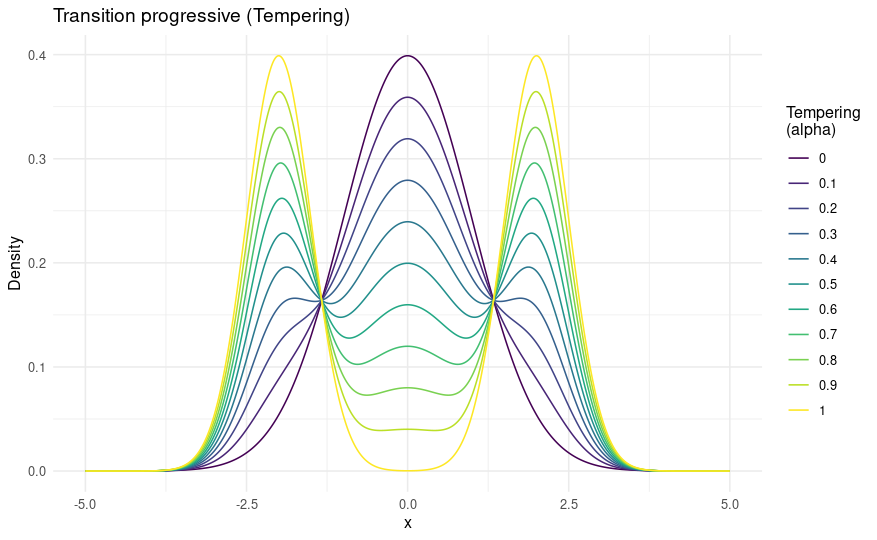
\includegraphics[scale=.8]{tempering.png}}
Tempering strategies
\begin{itemize}
\item Data tempering:
\item 
\item 
\end{itemize}
}
%%%%%%%%%%%%%%%%%%%%%%%%%%%%%%%%%%%%%%%%%%%%%%%%%%%
\def\blocksmc{
 \innerblock{Sequential Monte Carlo}{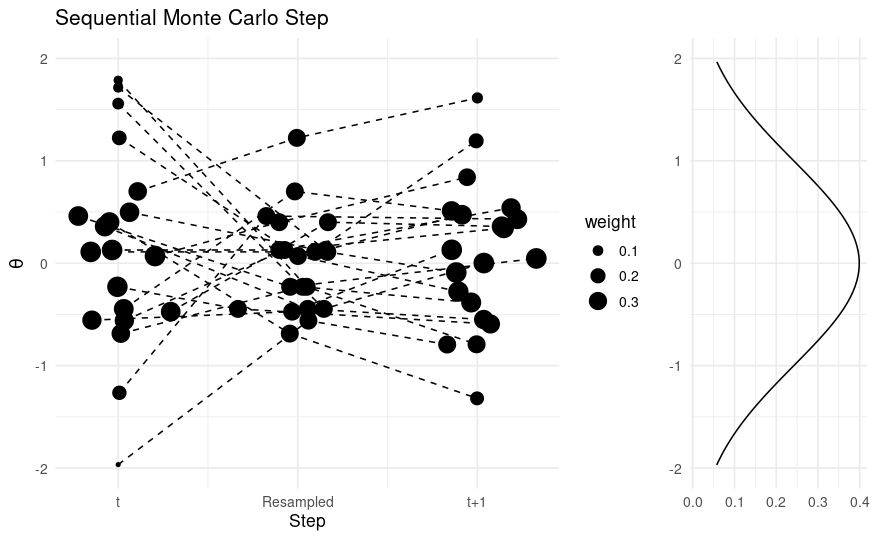
\includegraphics[scale=1]{smc.png}}}
%%%%%%%%%%%%%%%%%%%%%%%%%%%%%%%%%%%%%%%%%%%%%%%%%%%
\def\blockmodels{
\innerblock{Alternative models}{
 
 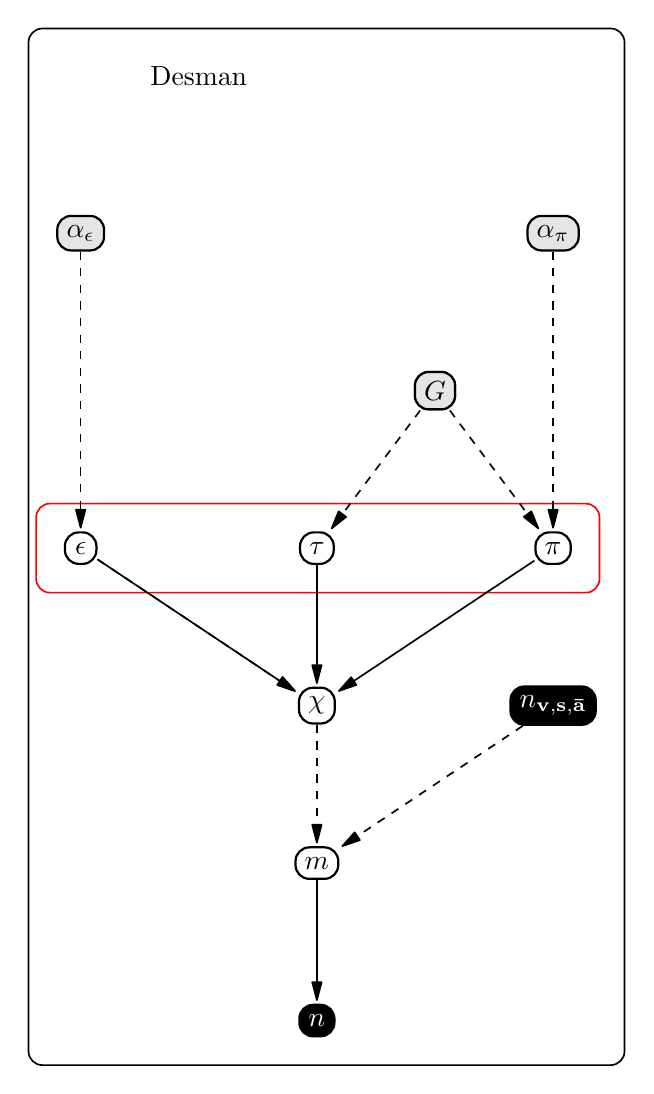
\begin{tikzpicture}[y=-2cm,x=3cm,
            > = {Stealth[inset=0pt,length=8pt,angle'=28,round]}, % arrow head style
            shorten > = 1pt, % don't touch arrow head to node
            auto,
%            node distance =1cm and 3cm, % distance between nodes
            semithick, % line style
            box/.style = {draw,red,inner sep=10pt,rounded corners=5pt}
        ]

        \tikzstyle{every state}=[
        rectangle,
        rounded corners=5pt,
            draw = black,
            thick,
            fill = white,
            minimum size = 4mm
        ]

 		\node at (1.5,1) (tt) {Desman};
        \node at (1.5,1) (blank) {};
        \node[state,fill=black!10] at (2.5,3) (G) {$G$};
        \node[state,fill=black!10] at (3,2) (alphapi) {$\alpha_\pi$};
        \node[state,fill=black!10] at (1,2) (alphaepsilon) {$\alpha_{\epsilon}$};
        \node[state] (tau) at (2,4) {$\tau$};
        \node[state] (epsilon) at (1,4) {$\epsilon$};
        \node[state] (pi) at (3,4) {$\pi$};
        \node[state] (chi) at (2,5) {$\chi$};
        %%\node (theta) at (0.5,4) {$\Theta$};
        \node[state,text=white,fill=black] (n) at (2,7) {$n$};
        \node[state,text=white,fill=black] (nvs) at (3,5)  {$n_{\indexvec{v},\indexvec{s},\indexsum{a}}$};
        \node[state] (m) at (2,6) {$\countdetail$};

         \node[box,fit=(tau) (pi) (epsilon)] {};
         
        \path[->,dashed] (alphapi) edge node {} (pi);
        \path[->,dashed] (alphaepsilon) edge node {} (epsilon);
        \path[->] (epsilon) edge node {} (chi);
        \path[->] (tau) edge node {} (chi);
        \path[->] (pi) edge node {} (chi);
        \path[->,dashed] (chi) edge node {} (m);
        \path[->,dashed] (epsilon) edge node {} (chi);
        \path[->,dashed] (nvs) edge node {} (m);
        \path[->,dashed] (G) edge node {} (tau);
        \path[->,dashed] (G) edge node {} (pi);
        \node[state,fill=black!10] at (2.5,3) (G) {$G$};
        \path[->] (m) edge node {} (n);
       
       
         \node[box,color=black,fit= (tt) (tau) (pi) (epsilon) (alphaepsilon) (m) (nvs) (n) (chi) (alphapi)] {};
        
    \end{tikzpicture}%
 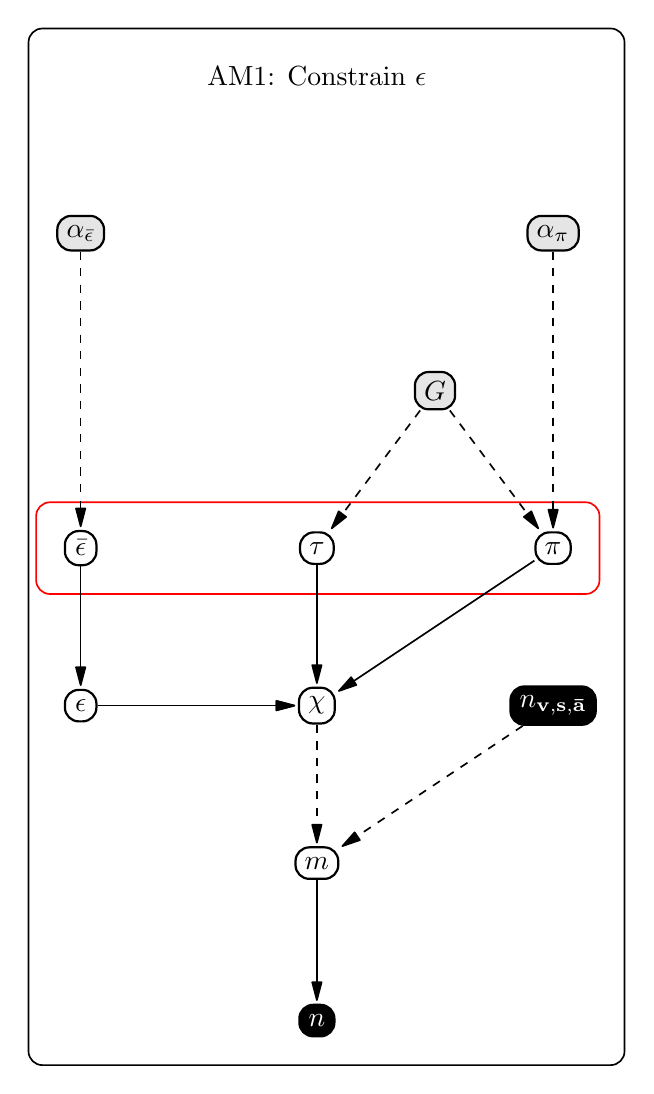
\begin{tikzpicture}[y=-2cm,x=3cm,
            > = {Stealth[inset=0pt,length=8pt,angle'=28,round]}, % arrow head style
            shorten > = 1pt, % don't touch arrow head to node
            auto,
%            node distance =1cm and 3cm, % distance between nodes
            semithick, % line style
            box/.style = {draw,red,inner sep=10pt,rounded corners=5pt}
        ]

        \tikzstyle{every state}=[
        rectangle,
        rounded corners=5pt,
            draw = black,
            thick,
            fill = white,
            minimum size = 4mm
        ]

        \node at (2,1) (tt) {AM1: Constrain $\epsilon$};
        \node at (1.5,1) (blank) {};

        \node[state,fill=black!10] at (2.5,3) (G) {$G$};
        \node[state,fill=black!10] at (3,2) (alphapi) {$\alpha_\pi$};
        \node[state,fill=black!10] at (1,2) (alphaepsilon) {$\alpha_{\bar\epsilon}$};
        \node[state] at (1,4) (barepsilon) {${\bar\epsilon}$};
        \node[state] (tau) at (2,4) {$\tau$};
        \node[state] (epsilon) at (1,5) {$\epsilon$};
        \node[state] (pi) at (3,4) {$\pi$};
        \node[state] (chi) at (2,5) {$\chi$};
        %%\node (theta) at (0.5,4) {$\Theta$};
        \node[state,text=white,fill=black] (n) at (2,7) {$n$};
        \node[state,text=white,fill=black] (nvs) at (3,5)  {$n_{\indexvec{v},\indexvec{s},\indexsum{a}}$};
        \node[state] (m) at (2,6) {$\countdetail$};

         \node[box,fit= (tau) (pi) (barepsilon)] {};
         
        \path[->,dashed] (alphapi) edge node {} (pi);
        \path[->,dashed] (alphaepsilon) edge node {} (barepsilon);
        \path[->] (barepsilon) edge node {} (epsilon);
        \path[->] (epsilon) edge node {} (chi);
        \path[->] (tau) edge node {} (chi);
        \path[->] (pi) edge node {} (chi);
        \path[->,dashed] (chi) edge node {} (m);
        \path[->] (epsilon) edge node {} (chi);
        \path[->,dashed] (nvs) edge node {} (m);
        \path[->] (m) edge node {} (n);
        \path[->,dashed] (G) edge node {} (tau);
        \path[->,dashed] (G) edge node {} (pi);
       
       
         \node[box,color=black,fit= (tt) (tau) (pi) (barepsilon) (alphaepsilon) (m) (nvs) (n) (chi) (alphapi)] {};
        
    \end{tikzpicture}%
 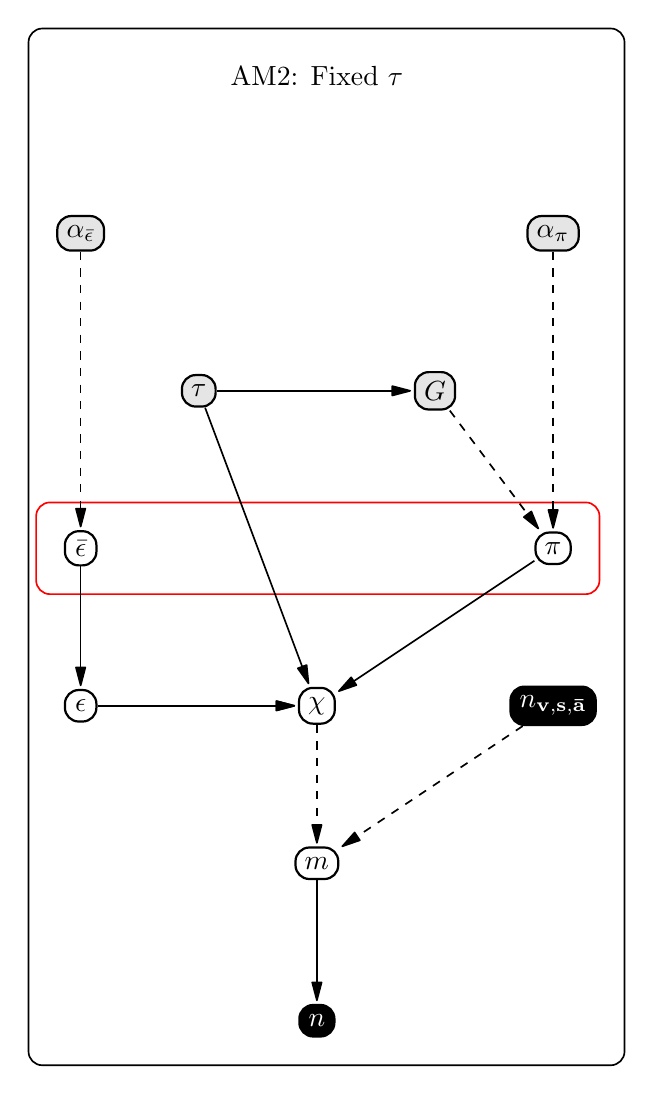
\begin{tikzpicture}[y=-2cm,x=3cm,
            > = {Stealth[inset=0pt,length=8pt,angle'=28,round]}, % arrow head style
            shorten > = 1pt, % don't touch arrow head to node
            auto,
%            node distance =1cm and 3cm, % distance between nodes
            semithick, % line style
            box/.style = {draw,red,inner sep=10pt,rounded corners=5pt}
        ]

        \tikzstyle{every state}=[
        rectangle,
        rounded corners=5pt,
            draw = black,
            thick,
            fill = white,
            minimum size = 4mm
        ]

        \node at (2,1) (tt) {AM2: Fixed $\tau$ };

        \node[state,fill=black!10] at (2.5,3) (G) {$G$};
        \node[state,fill=black!10] at (3,2) (alphapi) {$\alpha_\pi$};
        \node[state,fill=black!10] at (1,2) (alphaepsilon) {$\alpha_{\bar\epsilon}$};
        \node[state] at (1,4) (barepsilon) {${\bar\epsilon}$};
        \node[state,fill=black!10] (tau) at (1.5,3) {$\tau$};
        \node[state] (epsilon) at (1,5) {$\epsilon$};
        \node[state] (pi) at (3,4) {$\pi$};
        \node[state] (chi) at (2,5) {$\chi$};
        %\node (theta) at (0.5,4) {$\Theta$};
        \node[state,text=white,fill=black] (n) at (2,7) {$n$};
        \node[state,text=white,fill=black] (nvs) at (3,5)  {$n_{\indexvec{v},\indexvec{s},\indexsum{a}}$};
        \node[state] (m) at (2,6) {$\countdetail$};

         \node[box,fit=  (pi) (barepsilon)] {};
        \path[->,dashed] (alphapi) edge node {} (pi);
        \path[->,dashed] (alphaepsilon) edge node {} (barepsilon);
        \path[->] (barepsilon) edge node {} (epsilon);
        \path[->] (epsilon) edge node {} (chi);
        \path[->] (tau) edge node {} (chi);
        \path[->] (pi) edge node {} (chi);
        \path[->,dashed] (chi) edge node {} (m);
        \path[->] (epsilon) edge node {} (chi);
        \path[->,dashed] (nvs) edge node {} (m);
        \path[->] (m) edge node {} (n);
        \path[->] (tau) edge node {} (G);
        \path[->,dashed] (G) edge node {} (pi);
       
        
       
         \node[box,color=black,fit= (tt) (tau) (pi) (alphaepsilon) (alphapi) (m) (nvs) (n) (chi)] {};
    \end{tikzpicture}%
  \begin{tikzpicture}[y=-2cm,x=3cm,
            > = {Stealth[inset=0pt,length=8pt,angle'=28,round]}, % arrow head style
            shorten > = 1pt, % don't touch arrow head to node
            auto,
%            node distance =1cm and 3cm, % distance between nodes
            semithick, % line style
            box/.style = {draw,red,inner sep=10pt,rounded corners=5pt}
        ]

        \tikzstyle{every state}=[
        rectangle,
        rounded corners=5pt,
            draw = black,
            thick,
            fill = white,
            minimum size = 4mm
        ]


        \node at (2,0) (tt) {AM3: Relax $\rho$ };
        \node[state,fill=black!10] at (2.5,1.5) (G) {$G$};
        \node[state,fill=black!10] at (3,1) (alphapi) {$\alpha_\pi$};
        \node[state,fill=black!10] at (1.5,1) (alpharho) {$\alpha_\rho$};
        \node[state] (pi) at (3,3) {$\pi$};
        \node[state] (chi) at (1.75,4) {$\chi_{\indexvec{v},\indexvec{s},\indexvec{a},\indexsum{b},\indexvec{g}}$};
        \node[state] (rho) at (1.5,3) {$\tilde\rho$};
        \node[state] (tau) at (.5,4) {$\tau$};
        \node[state,text=white,fill=black] (n) at (2,6) {$n$};
        \node[state] (m) at (2,5) {$\countdetail_{\indexvec{v},\indexvec{s},\indexvec{a},\indexsum{b},\indexvec{g}}$};

        \node[state,text=white,fill=black] (nvs) at (3,4) {$n_{\indexvec{v},\indexvec{s},\indexsum{a}}$};
        
        \node[box,fit=(pi) (rho) ] {};
        \path[->,dashed] (alpharho) edge node {} (rho);
        \path[->,dashed] (alphapi) edge node {} (pi);
        \path[->] (pi) edge node {} (chi);
        \path[->] (rho) edge node {} (chi);
        \path[->,dashed] (chi) edge node {} (m);
        \path[->] (rho) edge node {} (tau);
        \path[->,dashed] (nvs) edge node {} (m);
        \path[->] (m) edge node {} (n);
        \path[->,dashed] (G) edge node {} (pi);
        \path[->,dashed] (G) edge node {} (rho);
        
        \node[box,color=black,fit= (tt) (tau) (pi) (alpharho) (alphaepsilon) (m) (nvs) (n) (chi)] {};
    \end{tikzpicture}%
 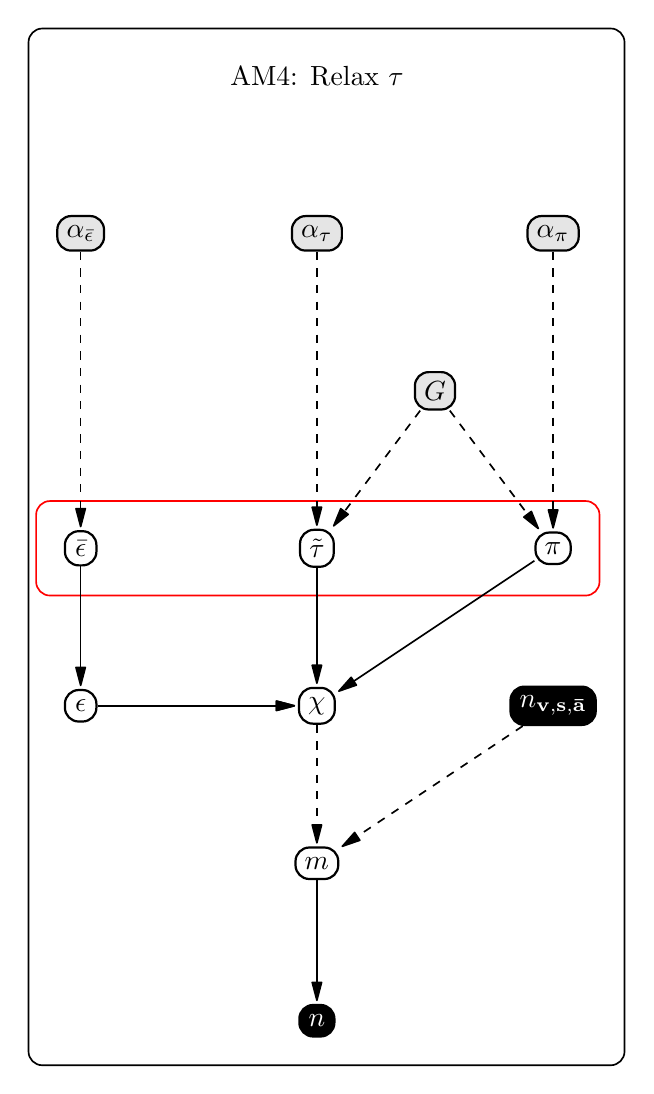
\begin{tikzpicture}[y=-2cm,x=3cm,
            > = {Stealth[inset=0pt,length=8pt,angle'=28,round]}, % arrow head style
            shorten > = 1pt, % don't touch arrow head to node
            auto,
%            node distance =1cm and 3cm, % distance between nodes
            semithick, % line style
            box/.style = {draw,red,inner sep=10pt,rounded corners=5pt}
        ]

        \tikzstyle{every state}=[
        rectangle,
        rounded corners=5pt,
            draw = black,
            thick,
            fill = white,
            minimum size = 4mm
        ]

        \node at (2,1) (tt) {AM4: Relax $\tau$ };
        \node at (1.5,1) (blank) {};

        \node[state,fill=black!10] at (2.5,3) (G) {$G$};
        \node[state,fill=black!10] at (2,2) (alphatau) {$\alpha_\tau$};
        \node[state,fill=black!10] at (3,2) (alphapi) {$\alpha_\pi$};
        \node[state,fill=black!10] at (1,2) (alphaepsilon) {$\alpha_{\bar\epsilon}$};
        \node[state] at (1,4) (barepsilon) {${\bar\epsilon}$};
        \node[state] (tau) at (2,4) {$\tilde\tau$};
        \node[state] (epsilon) at (1,5) {$\epsilon$};
        \node[state] (pi) at (3,4) {$\pi$};
        \node[state] (chi) at (2,5) {$\chi$};
        %\node (theta) at (0.5,4) {$\Theta$};
        \node[state,text=white,fill=black] (n) at (2,7) {$n$};
        \node[state,text=white,fill=black] (nvs) at (3,5)  {$n_{\indexvec{v},\indexvec{s},\indexsum{a}}$};
        \node[state] (m) at (2,6) {$\countdetail$};

         \node[box,fit= (tau) (pi) (barepsilon)] {};
        \path[->,dashed] (alphatau) edge node {} (tau);
        \path[->,dashed] (alphapi) edge node {} (pi);
        \path[->,dashed] (alphaepsilon) edge node {} (barepsilon);
        \path[->] (barepsilon) edge node {} (epsilon);
        \path[->] (epsilon) edge node {} (chi);
        \path[->] (tau) edge node {} (chi);
        \path[->] (pi) edge node {} (chi);
        \path[->,dashed] (chi) edge node {} (m);
        \path[->] (epsilon) edge node {} (chi);
        \path[->,dashed] (nvs) edge node {} (m);
        \path[->] (m) edge node {} (n);
        \path[->,dashed] (G) edge node {} (tau);
        \path[->,dashed] (G) edge node {} (pi);
       
         \node[box,color=black,fit= (tt) (tau) (pi) (barepsilon) (alphaepsilon) (m) (nvs) (n) (chi)] {};
        
    \end{tikzpicture}%
 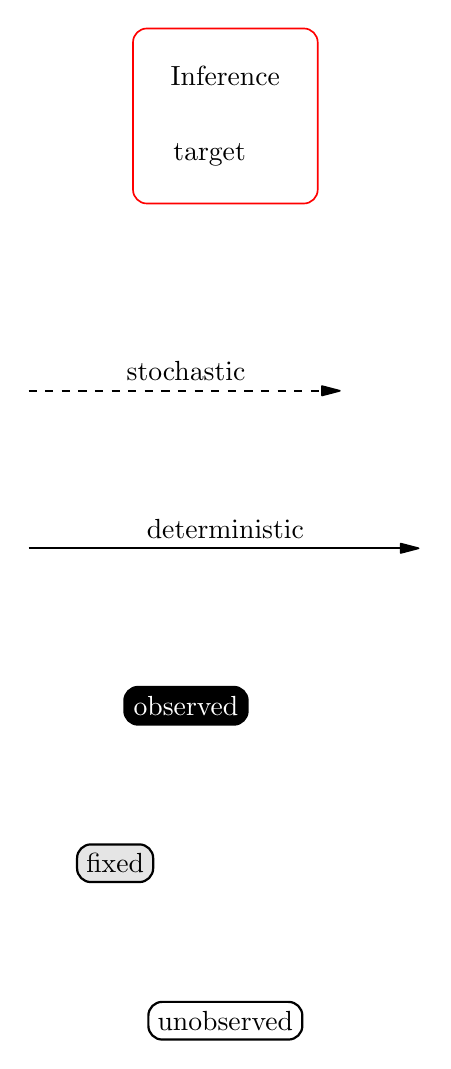
\begin{tikzpicture}[y=2cm,
            > = {Stealth[inset=0pt,length=8pt,angle'=28,round]}, % arrow head style
            shorten > = 1pt, % don't touch arrow head to node
            auto,
%            node distance =1cm and 3cm, % distance between nodes
            semithick, % line style
            box/.style = {draw,red,inner sep=10pt,rounded corners=5pt}
        ]

        \tikzstyle{every state}=[
        rectangle,
        rounded corners=5pt,
            draw = black,
            thick,
            fill = white,
            minimum size = 4mm
        ]

        \node[state,fill=black!10] at (1.1,1) (fixed) {fixed};
        \node[state] at (2.5,0)  (unobserved)  {unobserved};
        \node[state,text=white,fill=black ] at (2,2) (observed)  {observed};
        \path[->] (0,3) edge node {deterministic} (5,3);
        \path[->,dashed] (0,4) edge node {stochastic} (4,4);

        \node at (2.3,5.5) (theta1) {target};
        \node at (2.5,6) (theta2) {Inference};
        \node[box,fit=(theta1) (theta2)] {};
         \end{tikzpicture}
}}
%%%%%%%%%%%%%%%%%%%%%%%%%%%%%%%%%%%%%%%%%%%%%%%%%%%
\def\blockd{
\block{Alternative models and sampling strategies}{
\blockmodels
\innerblock{Relaxation}{
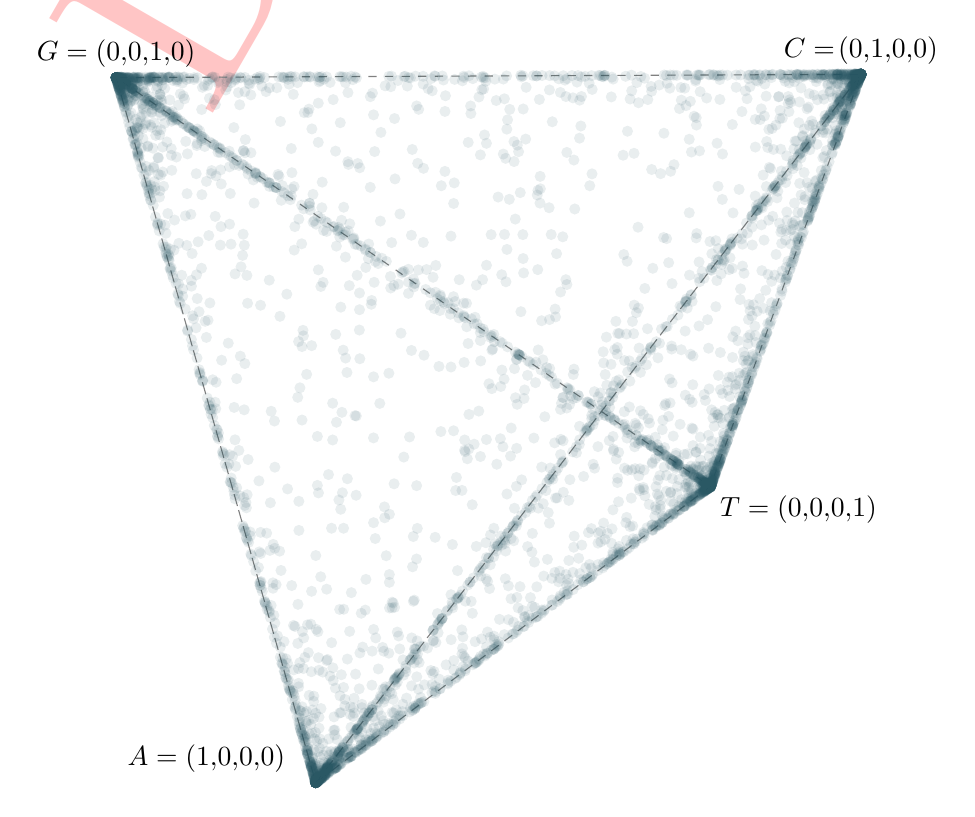
\begin{tikzpicture}[scale=10]


\begin{scope}[rotate around y=45,rotate around z=45]
 
% Draw the vertices of the tetrahedron

\coordinate (A) at (0, 0, 0);
\coordinate (C) at (1, 0, 0);
\coordinate (G) at (0.5, 0.866, 0);
\coordinate (T) at (0.5, 0.2887, 0.816);

%\foreach \p in {A,C,G,T}\fill[black] (\p) circle (0.02);

% Draw the edges of the cube
\draw[white!50!black, dashed]  (A) -- (C) -- (G) -- (A) -- (C) -- (T) -- (A) -- (T) -- (G) --  cycle;



    \pgfmathsetmacro{\alphaa}{0.1}       
       
\fill[color1,  opacity=\alphaa] (0.423,0.586,0.046) circle (.2pt);
         \fill[color1,  opacity=\alphaa] (0.984,0.027,0) circle (.2pt);
         \fill[color1,  opacity=\alphaa] (0.286,0.29,0.207) circle (.2pt);
         \fill[color1,  opacity=\alphaa] (0.842,0.106,0) circle (.2pt);
         \fill[color1,  opacity=\alphaa] (0.604,0.399,0.404) circle (.2pt);
         \fill[color1,  opacity=\alphaa] (0.093,0.02,0.057) circle (.2pt);
         \fill[color1,  opacity=\alphaa] (0,0,0) circle (.2pt);
         \fill[color1,  opacity=\alphaa] (0.231,0,0) circle (.2pt);
         \fill[color1,  opacity=\alphaa] (1,0,0) circle (.2pt);
         \fill[color1,  opacity=\alphaa] (0.36,0.556,0.003) circle (.2pt);
         \fill[color1,  opacity=\alphaa] (0.454,0.593,0.229) circle (.2pt);
         \fill[color1,  opacity=\alphaa] (0.506,0.85,0) circle (.2pt);
         \fill[color1,  opacity=\alphaa] (0.414,0.41,0.052) circle (.2pt);
         \fill[color1,  opacity=\alphaa] (0.533,0.269,0.762) circle (.2pt);
         \fill[color1,  opacity=\alphaa] (0.488,0.837,0) circle (.2pt);
         \fill[color1,  opacity=\alphaa] (0.001,0,0) circle (.2pt);
         \fill[color1,  opacity=\alphaa] (0.364,0.631,0) circle (.2pt);
         \fill[color1,  opacity=\alphaa] (0.495,0.836,0) circle (.2pt);
         \fill[color1,  opacity=\alphaa] (0.996,0.001,0) circle (.2pt);
         \fill[color1,  opacity=\alphaa] (0.999,0,0.001) circle (.2pt);
         \fill[color1,  opacity=\alphaa] (0.453,0.784,0) circle (.2pt);
         \fill[color1,  opacity=\alphaa] (0.405,0.235,0.66) circle (.2pt);
         \fill[color1,  opacity=\alphaa] (0.828,0.099,0.281) circle (.2pt);
         \fill[color1,  opacity=\alphaa] (0.648,0.186,0.526) circle (.2pt);
         \fill[color1,  opacity=\alphaa] (0.488,0.846,0) circle (.2pt);
         \fill[color1,  opacity=\alphaa] (0.47,0.438,0.499) circle (.2pt);
         \fill[color1,  opacity=\alphaa] (0.498,0.863,0) circle (.2pt);
         \fill[color1,  opacity=\alphaa] (0.006,0.01,0) circle (.2pt);
         \fill[color1,  opacity=\alphaa] (0.5,0.839,0.038) circle (.2pt);
         \fill[color1,  opacity=\alphaa] (0.605,0.051,0) circle (.2pt);
         \fill[color1,  opacity=\alphaa] (0.485,0.287,0.782) circle (.2pt);
         \fill[color1,  opacity=\alphaa] (0.516,0.502,0.418) circle (.2pt);
         \fill[color1,  opacity=\alphaa] (0.035,0.025,0.051) circle (.2pt);
         \fill[color1,  opacity=\alphaa] (0.5,0.289,0.816) circle (.2pt);
         \fill[color1,  opacity=\alphaa] (0.267,0.463,0) circle (.2pt);
         \fill[color1,  opacity=\alphaa] (0.5,0.289,0.816) circle (.2pt);
         \fill[color1,  opacity=\alphaa] (0.482,0.827,0) circle (.2pt);
         \fill[color1,  opacity=\alphaa] (0.5,0.298,0.804) circle (.2pt);
         \fill[color1,  opacity=\alphaa] (0.5,0.866,0) circle (.2pt);
         \fill[color1,  opacity=\alphaa] (0.5,0.289,0.816) circle (.2pt);
         \fill[color1,  opacity=\alphaa] (0.844,0.092,0.252) circle (.2pt);
         \fill[color1,  opacity=\alphaa] (0.476,0.583,0.341) circle (.2pt);
         \fill[color1,  opacity=\alphaa] (0.46,0.777,0.029) circle (.2pt);
         \fill[color1,  opacity=\alphaa] (0.996,0.007,0) circle (.2pt);
         \fill[color1,  opacity=\alphaa] (0.392,0.498,0.256) circle (.2pt);
         \fill[color1,  opacity=\alphaa] (0.977,0.013,0.038) circle (.2pt);
         \fill[color1,  opacity=\alphaa] (0.95,0.032,0.077) circle (.2pt);
         \fill[color1,  opacity=\alphaa] (0.436,0.611,0.002) circle (.2pt);
         \fill[color1,  opacity=\alphaa] (0.025,0.029,0.019) circle (.2pt);
         \fill[color1,  opacity=\alphaa] (0.952,0.028,0.079) circle (.2pt);
         \fill[color1,  opacity=\alphaa] (0.975,0.004,0.011) circle (.2pt);
         \fill[color1,  opacity=\alphaa] (0.006,0.002,0.006) circle (.2pt);
         \fill[color1,  opacity=\alphaa] (0.52,0.261,0.738) circle (.2pt);
         \fill[color1,  opacity=\alphaa] (0.319,0.184,0.521) circle (.2pt);
         \fill[color1,  opacity=\alphaa] (0.382,0.238,0.595) circle (.2pt);
         \fill[color1,  opacity=\alphaa] (0.207,0.357,0) circle (.2pt);
         \fill[color1,  opacity=\alphaa] (0.5,0.851,0.022) circle (.2pt);
         \fill[color1,  opacity=\alphaa] (0.575,0.22,0.616) circle (.2pt);
         \fill[color1,  opacity=\alphaa] (0.489,0.804,0.06) circle (.2pt);
         \fill[color1,  opacity=\alphaa] (0.968,0.006,0) circle (.2pt);
         \fill[color1,  opacity=\alphaa] (0.403,0,0) circle (.2pt);
         \fill[color1,  opacity=\alphaa] (0.008,0,0) circle (.2pt);
         \fill[color1,  opacity=\alphaa] (0.523,0.275,0.778) circle (.2pt);
         \fill[color1,  opacity=\alphaa] (0.5,0.474,0.554) circle (.2pt);
         \fill[color1,  opacity=\alphaa] (0.516,0.822,0.022) circle (.2pt);
         \fill[color1,  opacity=\alphaa] (0.021,0.001,0.003) circle (.2pt);
         \fill[color1,  opacity=\alphaa] (0.5,0.866,0) circle (.2pt);
         \fill[color1,  opacity=\alphaa] (0.339,0,0) circle (.2pt);
         \fill[color1,  opacity=\alphaa] (0.505,0.856,0.002) circle (.2pt);
         \fill[color1,  opacity=\alphaa] (0.002,0,0) circle (.2pt);
         \fill[color1,  opacity=\alphaa] (0.132,0.044,0.125) circle (.2pt);
         \fill[color1,  opacity=\alphaa] (0.508,0.851,0) circle (.2pt);
         \fill[color1,  opacity=\alphaa] (0,0,0) circle (.2pt);
         \fill[color1,  opacity=\alphaa] (0.831,0.29,0.003) circle (.2pt);
         \fill[color1,  opacity=\alphaa] (0,0,0) circle (.2pt);
         \fill[color1,  opacity=\alphaa] (0.502,0.301,0.793) circle (.2pt);
         \fill[color1,  opacity=\alphaa] (0.598,0.67,0.001) circle (.2pt);
         \fill[color1,  opacity=\alphaa] (0.5,0.846,0.028) circle (.2pt);
         \fill[color1,  opacity=\alphaa] (0.979,0.037,0) circle (.2pt);
         \fill[color1,  opacity=\alphaa] (0.548,0.78,0) circle (.2pt);
         \fill[color1,  opacity=\alphaa] (0.528,0.273,0.771) circle (.2pt);
         \fill[color1,  opacity=\alphaa] (0.445,0.769,0) circle (.2pt);
         \fill[color1,  opacity=\alphaa] (1,0,0) circle (.2pt);
         \fill[color1,  opacity=\alphaa] (0.461,0.264,0.748) circle (.2pt);
         \fill[color1,  opacity=\alphaa] (0.486,0.779,0.087) circle (.2pt);
         \fill[color1,  opacity=\alphaa] (0.074,0.018,0.034) circle (.2pt);
         \fill[color1,  opacity=\alphaa] (0.205,0.014,0.04) circle (.2pt);
         \fill[color1,  opacity=\alphaa] (0.501,0.288,0.815) circle (.2pt);
         \fill[color1,  opacity=\alphaa] (0.901,0.171,0) circle (.2pt);
         \fill[color1,  opacity=\alphaa] (0.5,0.305,0.793) circle (.2pt);
         \fill[color1,  opacity=\alphaa] (0.476,0.275,0.777) circle (.2pt);
         \fill[color1,  opacity=\alphaa] (0.563,0.749,0.011) circle (.2pt);
         \fill[color1,  opacity=\alphaa] (0.194,0.005,0.014) circle (.2pt);
         \fill[color1,  opacity=\alphaa] (0.5,0.289,0.816) circle (.2pt);
         \fill[color1,  opacity=\alphaa] (0.984,0,0) circle (.2pt);
         \fill[color1,  opacity=\alphaa] (0.97,0.016,0.013) circle (.2pt);
         \fill[color1,  opacity=\alphaa] (0.494,0.855,0) circle (.2pt);
         \fill[color1,  opacity=\alphaa] (0.497,0.287,0.811) circle (.2pt);
         \fill[color1,  opacity=\alphaa] (0.883,0.202,0) circle (.2pt);
         \fill[color1,  opacity=\alphaa] (0.305,0.055,0.001) circle (.2pt);
         \fill[color1,  opacity=\alphaa] (0.356,0.211,0.574) circle (.2pt);
         \fill[color1,  opacity=\alphaa] (0.02,0.035,0) circle (.2pt);
         \fill[color1,  opacity=\alphaa] (0.796,0.117,0.33) circle (.2pt);
         \fill[color1,  opacity=\alphaa] (0.391,0.161,0.43) circle (.2pt);
         \fill[color1,  opacity=\alphaa] (0.099,0.001,0) circle (.2pt);
         \fill[color1,  opacity=\alphaa] (0,0,0) circle (.2pt);
         \fill[color1,  opacity=\alphaa] (0.483,0.411,0.603) circle (.2pt);
         \fill[color1,  opacity=\alphaa] (0.5,0.289,0.816) circle (.2pt);
         \fill[color1,  opacity=\alphaa] (0.499,0.288,0.815) circle (.2pt);
         \fill[color1,  opacity=\alphaa] (0.499,0.864,0) circle (.2pt);
         \fill[color1,  opacity=\alphaa] (0.496,0.285,0.807) circle (.2pt);
         \fill[color1,  opacity=\alphaa] (0.493,0.852,0.002) circle (.2pt);
         \fill[color1,  opacity=\alphaa] (0.501,0.296,0.803) circle (.2pt);
         \fill[color1,  opacity=\alphaa] (0.155,0.26,0) circle (.2pt);
         \fill[color1,  opacity=\alphaa] (0.493,0.285,0.806) circle (.2pt);
         \fill[color1,  opacity=\alphaa] (0.581,0.14,0.377) circle (.2pt);
         \fill[color1,  opacity=\alphaa] (0.738,0,0) circle (.2pt);
         \fill[color1,  opacity=\alphaa] (0.655,0.199,0.563) circle (.2pt);
         \fill[color1,  opacity=\alphaa] (0.492,0.694,0.221) circle (.2pt);
         \fill[color1,  opacity=\alphaa] (0.502,0.86,0.004) circle (.2pt);
         \fill[color1,  opacity=\alphaa] (0.725,0.023,0.066) circle (.2pt);
         \fill[color1,  opacity=\alphaa] (0.029,0.049,0) circle (.2pt);
         \fill[color1,  opacity=\alphaa] (0.262,0,0) circle (.2pt);
         \fill[color1,  opacity=\alphaa] (0.382,0.368,0.414) circle (.2pt);
         \fill[color1,  opacity=\alphaa] (0.999,0.001,0.002) circle (.2pt);
         \fill[color1,  opacity=\alphaa] (0.5,0.313,0.783) circle (.2pt);
         \fill[color1,  opacity=\alphaa] (0.999,0,0) circle (.2pt);
         \fill[color1,  opacity=\alphaa] (0.496,0.858,0.001) circle (.2pt);
         \fill[color1,  opacity=\alphaa] (0.71,0.171,0.469) circle (.2pt);
         \fill[color1,  opacity=\alphaa] (0.025,0.014,0.041) circle (.2pt);
         \fill[color1,  opacity=\alphaa] (0.049,0,0) circle (.2pt);
         \fill[color1,  opacity=\alphaa] (0.439,0.15,0.424) circle (.2pt);
         \fill[color1,  opacity=\alphaa] (0.261,0.151,0.418) circle (.2pt);
         \fill[color1,  opacity=\alphaa] (0,0,0) circle (.2pt);
         \fill[color1,  opacity=\alphaa] (0.5,0.864,0.002) circle (.2pt);
         \fill[color1,  opacity=\alphaa] (0.347,0.427,0.242) circle (.2pt);
         \fill[color1,  opacity=\alphaa] (0.95,0.029,0.081) circle (.2pt);
         \fill[color1,  opacity=\alphaa] (1,0,0) circle (.2pt);
         \fill[color1,  opacity=\alphaa] (0.988,0.02,0) circle (.2pt);
         \fill[color1,  opacity=\alphaa] (0.784,0.124,0.35) circle (.2pt);
         \fill[color1,  opacity=\alphaa] (0.468,0.274,0.759) circle (.2pt);
         \fill[color1,  opacity=\alphaa] (0.286,0.093,0.263) circle (.2pt);
         \fill[color1,  opacity=\alphaa] (0.493,0.847,0.009) circle (.2pt);
         \fill[color1,  opacity=\alphaa] (0.927,0,0) circle (.2pt);
         \fill[color1,  opacity=\alphaa] (0.429,0,0) circle (.2pt);
         \fill[color1,  opacity=\alphaa] (0.916,0.047,0.133) circle (.2pt);
         \fill[color1,  opacity=\alphaa] (0.613,0,0.001) circle (.2pt);
         \fill[color1,  opacity=\alphaa] (0.5,0.327,0.763) circle (.2pt);
         \fill[color1,  opacity=\alphaa] (0.963,0.007,0) circle (.2pt);
         \fill[color1,  opacity=\alphaa] (0.534,0.268,0.759) circle (.2pt);
         \fill[color1,  opacity=\alphaa] (0.483,0.309,0.747) circle (.2pt);
         \fill[color1,  opacity=\alphaa] (0.499,0.865,0) circle (.2pt);
         \fill[color1,  opacity=\alphaa] (0.285,0.452,0.057) circle (.2pt);
         \fill[color1,  opacity=\alphaa] (0.848,0.088,0.247) circle (.2pt);
         \fill[color1,  opacity=\alphaa] (0.118,0.203,0.003) circle (.2pt);
         \fill[color1,  opacity=\alphaa] (1,0,0) circle (.2pt);
         \fill[color1,  opacity=\alphaa] (0.261,0.018,0.05) circle (.2pt);
         \fill[color1,  opacity=\alphaa] (0.5,0.866,0) circle (.2pt);
         \fill[color1,  opacity=\alphaa] (0.5,0.339,0.744) circle (.2pt);
         \fill[color1,  opacity=\alphaa] (0.066,0.113,0) circle (.2pt);
         \fill[color1,  opacity=\alphaa] (0.507,0.285,0.806) circle (.2pt);
         \fill[color1,  opacity=\alphaa] (0.023,0.004,0.01) circle (.2pt);
         \fill[color1,  opacity=\alphaa] (0.139,0.148,0) circle (.2pt);
         \fill[color1,  opacity=\alphaa] (0.507,0.332,0.74) circle (.2pt);
         \fill[color1,  opacity=\alphaa] (0.5,0.865,0.001) circle (.2pt);
         \fill[color1,  opacity=\alphaa] (0.5,0.301,0.799) circle (.2pt);
         \fill[color1,  opacity=\alphaa] (0.012,0.021,0) circle (.2pt);
         \fill[color1,  opacity=\alphaa] (0.459,0.767,0) circle (.2pt);
         \fill[color1,  opacity=\alphaa] (0.779,0.128,0.36) circle (.2pt);
         \fill[color1,  opacity=\alphaa] (0.5,0.699,0.236) circle (.2pt);
         \fill[color1,  opacity=\alphaa] (0.868,0.229,0) circle (.2pt);
         \fill[color1,  opacity=\alphaa] (0.004,0,0) circle (.2pt);
         \fill[color1,  opacity=\alphaa] (0.5,0.663,0.288) circle (.2pt);
         \fill[color1,  opacity=\alphaa] (0.496,0.507,0.498) circle (.2pt);
         \fill[color1,  opacity=\alphaa] (0.184,0.289,0.043) circle (.2pt);
         \fill[color1,  opacity=\alphaa] (0.5,0.863,0.004) circle (.2pt);
         \fill[color1,  opacity=\alphaa] (0.955,0.032,0.066) circle (.2pt);
         \fill[color1,  opacity=\alphaa] (0.484,0.838,0.002) circle (.2pt);
         \fill[color1,  opacity=\alphaa] (0.043,0.074,0) circle (.2pt);
         \fill[color1,  opacity=\alphaa] (0.501,0.31,0.784) circle (.2pt);
         \fill[color1,  opacity=\alphaa] (0.992,0.009,0) circle (.2pt);
         \fill[color1,  opacity=\alphaa] (0.491,0.851,0) circle (.2pt);
         \fill[color1,  opacity=\alphaa] (0.499,0.291,0.809) circle (.2pt);
         \fill[color1,  opacity=\alphaa] (0,0,0) circle (.2pt);
         \fill[color1,  opacity=\alphaa] (0.047,0.012,0.033) circle (.2pt);
         \fill[color1,  opacity=\alphaa] (0.961,0.067,0) circle (.2pt);
         \fill[color1,  opacity=\alphaa] (0.502,0.287,0.813) circle (.2pt);
         \fill[color1,  opacity=\alphaa] (0.499,0.288,0.814) circle (.2pt);
         \fill[color1,  opacity=\alphaa] (0.181,0.161,0) circle (.2pt);
         \fill[color1,  opacity=\alphaa] (0.455,0.783,0.001) circle (.2pt);
         \fill[color1,  opacity=\alphaa] (0.875,0,0) circle (.2pt);
         \fill[color1,  opacity=\alphaa] (0.505,0.304,0.782) circle (.2pt);
         \fill[color1,  opacity=\alphaa] (0.66,0.221,0.519) circle (.2pt);
         \fill[color1,  opacity=\alphaa] (0.564,0.252,0.712) circle (.2pt);
         \fill[color1,  opacity=\alphaa] (0.5,0.289,0.816) circle (.2pt);
         \fill[color1,  opacity=\alphaa] (0.5,0.289,0.816) circle (.2pt);
         \fill[color1,  opacity=\alphaa] (0.667,0.325,0.355) circle (.2pt);
         \fill[color1,  opacity=\alphaa] (1,0,0) circle (.2pt);
         \fill[color1,  opacity=\alphaa] (0.406,0.454,0.29) circle (.2pt);
         \fill[color1,  opacity=\alphaa] (0.55,0.776,0.004) circle (.2pt);
         \fill[color1,  opacity=\alphaa] (0.309,0.179,0.505) circle (.2pt);
         \fill[color1,  opacity=\alphaa] (0.5,0.861,0.007) circle (.2pt);
         \fill[color1,  opacity=\alphaa] (0.47,0.723,0.127) circle (.2pt);
         \fill[color1,  opacity=\alphaa] (0.061,0.03,0.083) circle (.2pt);
         \fill[color1,  opacity=\alphaa] (1,0,0) circle (.2pt);
         \fill[color1,  opacity=\alphaa] (0.5,0.288,0.816) circle (.2pt);
         \fill[color1,  opacity=\alphaa] (0.001,0,0) circle (.2pt);
         \fill[color1,  opacity=\alphaa] (0.5,0.865,0) circle (.2pt);
         \fill[color1,  opacity=\alphaa] (0.883,0.203,0) circle (.2pt);
         \fill[color1,  opacity=\alphaa] (0.224,0,0) circle (.2pt);
         \fill[color1,  opacity=\alphaa] (0.849,0.234,0) circle (.2pt);
         \fill[color1,  opacity=\alphaa] (0.484,0,0) circle (.2pt);
         \fill[color1,  opacity=\alphaa] (0.732,0.154,0.437) circle (.2pt);
         \fill[color1,  opacity=\alphaa] (0.998,0.001,0.004) circle (.2pt);
         \fill[color1,  opacity=\alphaa] (0.46,0.424,0.526) circle (.2pt);
         \fill[color1,  opacity=\alphaa] (0.524,0.825,0) circle (.2pt);
         \fill[color1,  opacity=\alphaa] (0.531,0.026,0.054) circle (.2pt);
         \fill[color1,  opacity=\alphaa] (0.022,0.001,0) circle (.2pt);
         \fill[color1,  opacity=\alphaa] (0.733,0.037,0.099) circle (.2pt);
         \fill[color1,  opacity=\alphaa] (0.5,0.339,0.745) circle (.2pt);
         \fill[color1,  opacity=\alphaa] (0.993,0.013,0) circle (.2pt);
         \fill[color1,  opacity=\alphaa] (0.5,0.857,0.013) circle (.2pt);
         \fill[color1,  opacity=\alphaa] (0.995,0.001,0.001) circle (.2pt);
         \fill[color1,  opacity=\alphaa] (0.075,0.103,0.039) circle (.2pt);
         \fill[color1,  opacity=\alphaa] (0.994,0.003,0.009) circle (.2pt);
         \fill[color1,  opacity=\alphaa] (0.855,0.021,0) circle (.2pt);
         \fill[color1,  opacity=\alphaa] (0.5,0.856,0.014) circle (.2pt);
         \fill[color1,  opacity=\alphaa] (0.995,0.003,0.008) circle (.2pt);
         \fill[color1,  opacity=\alphaa] (1,0,0) circle (.2pt);
         \fill[color1,  opacity=\alphaa] (0.002,0.001,0) circle (.2pt);
         \fill[color1,  opacity=\alphaa] (0.994,0,0.001) circle (.2pt);
         \fill[color1,  opacity=\alphaa] (0.493,0.281,0.794) circle (.2pt);
         \fill[color1,  opacity=\alphaa] (0.825,0.303,0) circle (.2pt);
         \fill[color1,  opacity=\alphaa] (0.501,0.859,0.008) circle (.2pt);
         \fill[color1,  opacity=\alphaa] (0.496,0.286,0.808) circle (.2pt);
         \fill[color1,  opacity=\alphaa] (0.497,0.283,0.799) circle (.2pt);
         \fill[color1,  opacity=\alphaa] (0.501,0.288,0.814) circle (.2pt);
         \fill[color1,  opacity=\alphaa] (0.502,0.298,0.798) circle (.2pt);
         \fill[color1,  opacity=\alphaa] (0.229,0.059,0.017) circle (.2pt);
         \fill[color1,  opacity=\alphaa] (0.5,0.858,0.011) circle (.2pt);
         \fill[color1,  opacity=\alphaa] (0.5,0.866,0) circle (.2pt);
         \fill[color1,  opacity=\alphaa] (0.17,0.06,0) circle (.2pt);
         \fill[color1,  opacity=\alphaa] (0.398,0.686,0.006) circle (.2pt);
         \fill[color1,  opacity=\alphaa] (0.949,0.071,0) circle (.2pt);
         \fill[color1,  opacity=\alphaa] (0.5,0.289,0.816) circle (.2pt);
         \fill[color1,  opacity=\alphaa] (0.976,0.03,0) circle (.2pt);
         \fill[color1,  opacity=\alphaa] (0.286,0.109,0.003) circle (.2pt);
         \fill[color1,  opacity=\alphaa] (0.002,0.001,0.002) circle (.2pt);
         \fill[color1,  opacity=\alphaa] (0.345,0.559,0) circle (.2pt);
         \fill[color1,  opacity=\alphaa] (0.456,0.633,0.219) circle (.2pt);
         \fill[color1,  opacity=\alphaa] (0.499,0.833,0.045) circle (.2pt);
         \fill[color1,  opacity=\alphaa] (0.01,0.005,0.002) circle (.2pt);
         \fill[color1,  opacity=\alphaa] (0.491,0.33,0.735) circle (.2pt);
         \fill[color1,  opacity=\alphaa] (0.554,0.752,0) circle (.2pt);
         \fill[color1,  opacity=\alphaa] (0.493,0.854,0) circle (.2pt);
         \fill[color1,  opacity=\alphaa] (0.999,0.001,0) circle (.2pt);
         \fill[color1,  opacity=\alphaa] (0.984,0.028,0) circle (.2pt);
         \fill[color1,  opacity=\alphaa] (0.999,0,0) circle (.2pt);
         \fill[color1,  opacity=\alphaa] (0.071,0.041,0.117) circle (.2pt);
         \fill[color1,  opacity=\alphaa] (0,0,0) circle (.2pt);
         \fill[color1,  opacity=\alphaa] (0.572,0.649,0.13) circle (.2pt);
         \fill[color1,  opacity=\alphaa] (0.406,0.235,0.662) circle (.2pt);
         \fill[color1,  opacity=\alphaa] (0.001,0.001,0.001) circle (.2pt);
         \fill[color1,  opacity=\alphaa] (0.998,0.001,0.003) circle (.2pt);
         \fill[color1,  opacity=\alphaa] (0.334,0,0) circle (.2pt);
         \fill[color1,  opacity=\alphaa] (0.989,0,0) circle (.2pt);
         \fill[color1,  opacity=\alphaa] (0.716,0.485,0.005) circle (.2pt);
         \fill[color1,  opacity=\alphaa] (0.002,0.004,0) circle (.2pt);
         \fill[color1,  opacity=\alphaa] (0.948,0.033,0.08) circle (.2pt);
         \fill[color1,  opacity=\alphaa] (0.996,0.002,0.007) circle (.2pt);
         \fill[color1,  opacity=\alphaa] (0.03,0.048,0) circle (.2pt);
         \fill[color1,  opacity=\alphaa] (0.503,0.335,0.744) circle (.2pt);
         \fill[color1,  opacity=\alphaa] (0.241,0.001,0) circle (.2pt);
         \fill[color1,  opacity=\alphaa] (0.063,0,0) circle (.2pt);
         \fill[color1,  opacity=\alphaa] (0.5,0.289,0.816) circle (.2pt);
         \fill[color1,  opacity=\alphaa] (0,0,0) circle (.2pt);
         \fill[color1,  opacity=\alphaa] (0.026,0,0) circle (.2pt);
         \fill[color1,  opacity=\alphaa] (0.021,0.037,0) circle (.2pt);
         \fill[color1,  opacity=\alphaa] (0.511,0.836,0.013) circle (.2pt);
         \fill[color1,  opacity=\alphaa] (0.953,0.027,0.076) circle (.2pt);
         \fill[color1,  opacity=\alphaa] (0.013,0,0) circle (.2pt);
         \fill[color1,  opacity=\alphaa] (0.452,0.288,0.7) circle (.2pt);
         \fill[color1,  opacity=\alphaa] (0.004,0.002,0.006) circle (.2pt);
         \fill[color1,  opacity=\alphaa] (0.455,0.055,0) circle (.2pt);
         \fill[color1,  opacity=\alphaa] (0.775,0.13,0.367) circle (.2pt);
         \fill[color1,  opacity=\alphaa] (0.5,0.289,0.816) circle (.2pt);
         \fill[color1,  opacity=\alphaa] (0.841,0,0) circle (.2pt);
         \fill[color1,  opacity=\alphaa] (0.732,0.004,0.009) circle (.2pt);
         \fill[color1,  opacity=\alphaa] (0.488,0.282,0.797) circle (.2pt);
         \fill[color1,  opacity=\alphaa] (0.003,0.005,0) circle (.2pt);
         \fill[color1,  opacity=\alphaa] (0.5,0.866,0.001) circle (.2pt);
         \fill[color1,  opacity=\alphaa] (0.513,0.281,0.796) circle (.2pt);
         \fill[color1,  opacity=\alphaa] (0.497,0.31,0.778) circle (.2pt);
         \fill[color1,  opacity=\alphaa] (0.83,0.289,0.007) circle (.2pt);
         \fill[color1,  opacity=\alphaa] (0.501,0.288,0.814) circle (.2pt);
         \fill[color1,  opacity=\alphaa] (0.5,0.29,0.815) circle (.2pt);
         \fill[color1,  opacity=\alphaa] (0.971,0.02,0.041) circle (.2pt);
         \fill[color1,  opacity=\alphaa] (0,0,0) circle (.2pt);
         \fill[color1,  opacity=\alphaa] (0.513,0.82,0.034) circle (.2pt);
         \fill[color1,  opacity=\alphaa] (0.518,0.67,0.234) circle (.2pt);
         \fill[color1,  opacity=\alphaa] (0.989,0.006,0.018) circle (.2pt);
         \fill[color1,  opacity=\alphaa] (1,0,0) circle (.2pt);
         \fill[color1,  opacity=\alphaa] (0.5,0.854,0.017) circle (.2pt);
         \fill[color1,  opacity=\alphaa] (0.501,0.797,0.059) circle (.2pt);
         \fill[color1,  opacity=\alphaa] (0.783,0.139,0.335) circle (.2pt);
         \fill[color1,  opacity=\alphaa] (0.194,0.135,0.01) circle (.2pt);
         \fill[color1,  opacity=\alphaa] (0.504,0.86,0) circle (.2pt);
         \fill[color1,  opacity=\alphaa] (0.915,0.049,0.139) circle (.2pt);
         \fill[color1,  opacity=\alphaa] (0.006,0.003,0.01) circle (.2pt);
         \fill[color1,  opacity=\alphaa] (0.5,0.393,0.669) circle (.2pt);
         \fill[color1,  opacity=\alphaa] (0.001,0,0.001) circle (.2pt);
         \fill[color1,  opacity=\alphaa] (0.916,0.089,0.065) circle (.2pt);
         \fill[color1,  opacity=\alphaa] (0.003,0,0) circle (.2pt);
         \fill[color1,  opacity=\alphaa] (0.552,0.216,0.612) circle (.2pt);
         \fill[color1,  opacity=\alphaa] (0.987,0.023,0) circle (.2pt);
         \fill[color1,  opacity=\alphaa] (0.883,0,0) circle (.2pt);
         \fill[color1,  opacity=\alphaa] (0.362,0,0) circle (.2pt);
         \fill[color1,  opacity=\alphaa] (0.952,0.003,0.003) circle (.2pt);
         \fill[color1,  opacity=\alphaa] (0.091,0.151,0.009) circle (.2pt);
         \fill[color1,  opacity=\alphaa] (0.426,0.733,0.007) circle (.2pt);
         \fill[color1,  opacity=\alphaa] (0.5,0.861,0.007) circle (.2pt);
         \fill[color1,  opacity=\alphaa] (0.5,0.289,0.816) circle (.2pt);
         \fill[color1,  opacity=\alphaa] (0.62,0.658,0) circle (.2pt);
         \fill[color1,  opacity=\alphaa] (0.785,0.341,0.044) circle (.2pt);
         \fill[color1,  opacity=\alphaa] (0.004,0.007,0) circle (.2pt);
         \fill[color1,  opacity=\alphaa] (0.702,0.185,0.416) circle (.2pt);
         \fill[color1,  opacity=\alphaa] (0.071,0.041,0.116) circle (.2pt);
         \fill[color1,  opacity=\alphaa] (0.498,0.311,0.781) circle (.2pt);
         \fill[color1,  opacity=\alphaa] (0.499,0.86,0.006) circle (.2pt);
         \fill[color1,  opacity=\alphaa] (0.508,0.85,0) circle (.2pt);
         \fill[color1,  opacity=\alphaa] (0.006,0,0) circle (.2pt);
         \fill[color1,  opacity=\alphaa] (0.523,0.826,0) circle (.2pt);
         \fill[color1,  opacity=\alphaa] (0.001,0,0) circle (.2pt);
         \fill[color1,  opacity=\alphaa] (0.49,0.087,0.243) circle (.2pt);
         \fill[color1,  opacity=\alphaa] (0.5,0.857,0.013) circle (.2pt);
         \fill[color1,  opacity=\alphaa] (0.5,0.771,0.134) circle (.2pt);
         \fill[color1,  opacity=\alphaa] (0.444,0.365,0.572) circle (.2pt);
         \fill[color1,  opacity=\alphaa] (0.313,0.175,0.494) circle (.2pt);
         \fill[color1,  opacity=\alphaa] (0.497,0.287,0.812) circle (.2pt);
         \fill[color1,  opacity=\alphaa] (0.167,0.096,0.273) circle (.2pt);
         \fill[color1,  opacity=\alphaa] (0.5,0.528,0.477) circle (.2pt);
         \fill[color1,  opacity=\alphaa] (0.473,0.791,0.039) circle (.2pt);
         \fill[color1,  opacity=\alphaa] (0.892,0.187,0) circle (.2pt);
         \fill[color1,  opacity=\alphaa] (0.187,0.003,0) circle (.2pt);
         \fill[color1,  opacity=\alphaa] (0.497,0.857,0) circle (.2pt);
         \fill[color1,  opacity=\alphaa] (1,0,0) circle (.2pt);
         \fill[color1,  opacity=\alphaa] (0.031,0.018,0.051) circle (.2pt);
         \fill[color1,  opacity=\alphaa] (0.495,0.857,0) circle (.2pt);
         \fill[color1,  opacity=\alphaa] (0.807,0.3,0) circle (.2pt);
         \fill[color1,  opacity=\alphaa] (0.226,0.131,0.37) circle (.2pt);
         \fill[color1,  opacity=\alphaa] (0.984,0,0) circle (.2pt);
         \fill[color1,  opacity=\alphaa] (0.498,0.288,0.813) circle (.2pt);
         \fill[color1,  opacity=\alphaa] (0.011,0.019,0) circle (.2pt);
         \fill[color1,  opacity=\alphaa] (0.5,0.289,0.816) circle (.2pt);
         \fill[color1,  opacity=\alphaa] (0.936,0.11,0) circle (.2pt);
         \fill[color1,  opacity=\alphaa] (0.491,0.283,0.801) circle (.2pt);
         \fill[color1,  opacity=\alphaa] (0.419,0.242,0.675) circle (.2pt);
         \fill[color1,  opacity=\alphaa] (0.538,0.267,0.754) circle (.2pt);
         \fill[color1,  opacity=\alphaa] (0.501,0.288,0.814) circle (.2pt);
         \fill[color1,  opacity=\alphaa] (0.5,0.355,0.722) circle (.2pt);
         \fill[color1,  opacity=\alphaa] (0,0.001,0) circle (.2pt);
         \fill[color1,  opacity=\alphaa] (0.286,0.165,0.467) circle (.2pt);
         \fill[color1,  opacity=\alphaa] (0.5,0.67,0.277) circle (.2pt);
         \fill[color1,  opacity=\alphaa] (0.03,0,0) circle (.2pt);
         \fill[color1,  opacity=\alphaa] (0.072,0.035,0.099) circle (.2pt);
         \fill[color1,  opacity=\alphaa] (0.491,0.283,0.8) circle (.2pt);
         \fill[color1,  opacity=\alphaa] (0.113,0.146,0) circle (.2pt);
         \fill[color1,  opacity=\alphaa] (0.5,0.445,0.594) circle (.2pt);
         \fill[color1,  opacity=\alphaa] (0.246,0.426,0) circle (.2pt);
         \fill[color1,  opacity=\alphaa] (0.528,0.219,0.618) circle (.2pt);
         \fill[color1,  opacity=\alphaa] (0.985,0.012,0.021) circle (.2pt);
         \fill[color1,  opacity=\alphaa] (0.503,0.291,0.803) circle (.2pt);
         \fill[color1,  opacity=\alphaa] (0.5,0.85,0.023) circle (.2pt);
         \fill[color1,  opacity=\alphaa] (0.201,0.339,0.012) circle (.2pt);
         \fill[color1,  opacity=\alphaa] (0.5,0.766,0.141) circle (.2pt);
         \fill[color1,  opacity=\alphaa] (0.069,0.075,0.063) circle (.2pt);
         \fill[color1,  opacity=\alphaa] (0.999,0,0.001) circle (.2pt);
         \fill[color1,  opacity=\alphaa] (0.722,0.161,0.454) circle (.2pt);
         \fill[color1,  opacity=\alphaa] (0.501,0.3,0.798) circle (.2pt);
         \fill[color1,  opacity=\alphaa] (0.264,0.153,0.432) circle (.2pt);
         \fill[color1,  opacity=\alphaa] (0.077,0,0) circle (.2pt);
         \fill[color1,  opacity=\alphaa] (0.812,0.088,0.239) circle (.2pt);
         \fill[color1,  opacity=\alphaa] (0.565,0.488,0.376) circle (.2pt);
         \fill[color1,  opacity=\alphaa] (0.968,0.055,0) circle (.2pt);
         \fill[color1,  opacity=\alphaa] (0,0,0.001) circle (.2pt);
         \fill[color1,  opacity=\alphaa] (0.526,0.822,0) circle (.2pt);
         \fill[color1,  opacity=\alphaa] (0.467,0.27,0.762) circle (.2pt);
         \fill[color1,  opacity=\alphaa] (0.025,0,0) circle (.2pt);
         \fill[color1,  opacity=\alphaa] (0.5,0.325,0.765) circle (.2pt);
         \fill[color1,  opacity=\alphaa] (0.257,0.301,0.143) circle (.2pt);
         \fill[color1,  opacity=\alphaa] (0.009,0,0.001) circle (.2pt);
         \fill[color1,  opacity=\alphaa] (0.686,0.53,0.019) circle (.2pt);
         \fill[color1,  opacity=\alphaa] (0.5,0.866,0) circle (.2pt);
         \fill[color1,  opacity=\alphaa] (0.735,0.191,0.38) circle (.2pt);
         \fill[color1,  opacity=\alphaa] (0.499,0.864,0) circle (.2pt);
         \fill[color1,  opacity=\alphaa] (0,0,0) circle (.2pt);
         \fill[color1,  opacity=\alphaa] (0.971,0.051,0) circle (.2pt);
         \fill[color1,  opacity=\alphaa] (0.934,0.047,0) circle (.2pt);
         \fill[color1,  opacity=\alphaa] (0.5,0.501,0.517) circle (.2pt);
         \fill[color1,  opacity=\alphaa] (0.125,0.189,0.037) circle (.2pt);
         \fill[color1,  opacity=\alphaa] (0.5,0.861,0.006) circle (.2pt);
         \fill[color1,  opacity=\alphaa] (0.5,0.788,0.109) circle (.2pt);
         \fill[color1,  opacity=\alphaa] (0.003,0.003,0.002) circle (.2pt);
         \fill[color1,  opacity=\alphaa] (0.501,0.865,0) circle (.2pt);
         \fill[color1,  opacity=\alphaa] (0.931,0.072,0.012) circle (.2pt);
         \fill[color1,  opacity=\alphaa] (0.5,0.865,0) circle (.2pt);
         \fill[color1,  opacity=\alphaa] (1,0.001,0) circle (.2pt);
         \fill[color1,  opacity=\alphaa] (0.004,0.007,0) circle (.2pt);
         \fill[color1,  opacity=\alphaa] (0.237,0.395,0) circle (.2pt);
         \fill[color1,  opacity=\alphaa] (0.499,0.294,0.807) circle (.2pt);
         \fill[color1,  opacity=\alphaa] (0.516,0.28,0.791) circle (.2pt);
         \fill[color1,  opacity=\alphaa] (0.461,0.172,0.486) circle (.2pt);
         \fill[color1,  opacity=\alphaa] (0.454,0.262,0.741) circle (.2pt);
         \fill[color1,  opacity=\alphaa] (0.013,0,0) circle (.2pt);
         \fill[color1,  opacity=\alphaa] (0.409,0.238,0.665) circle (.2pt);
         \fill[color1,  opacity=\alphaa] (0.5,0.866,0) circle (.2pt);
         \fill[color1,  opacity=\alphaa] (0.485,0.363,0.674) circle (.2pt);
         \fill[color1,  opacity=\alphaa] (0.489,0.417,0.608) circle (.2pt);
         \fill[color1,  opacity=\alphaa] (1,0,0) circle (.2pt);
         \fill[color1,  opacity=\alphaa] (0.001,0.001,0) circle (.2pt);
         \fill[color1,  opacity=\alphaa] (0.497,0.287,0.812) circle (.2pt);
         \fill[color1,  opacity=\alphaa] (0.037,0.005,0.014) circle (.2pt);
         \fill[color1,  opacity=\alphaa] (0.85,0.084,0.237) circle (.2pt);
         \fill[color1,  opacity=\alphaa] (0.46,0.537,0.286) circle (.2pt);
         \fill[color1,  opacity=\alphaa] (0.5,0.289,0.816) circle (.2pt);
         \fill[color1,  opacity=\alphaa] (0.5,0.289,0.816) circle (.2pt);
         \fill[color1,  opacity=\alphaa] (0.488,0.843,0.003) circle (.2pt);
         \fill[color1,  opacity=\alphaa] (0.482,0.278,0.783) circle (.2pt);
         \fill[color1,  opacity=\alphaa] (0.54,0.318,0.677) circle (.2pt);
         \fill[color1,  opacity=\alphaa] (0.5,0.289,0.816) circle (.2pt);
         \fill[color1,  opacity=\alphaa] (0.491,0.808,0) circle (.2pt);
         \fill[color1,  opacity=\alphaa] (0.727,0,0) circle (.2pt);
         \fill[color1,  opacity=\alphaa] (0,0,0) circle (.2pt);
         \fill[color1,  opacity=\alphaa] (0.699,0.174,0.491) circle (.2pt);
         \fill[color1,  opacity=\alphaa] (0,0,0) circle (.2pt);
         \fill[color1,  opacity=\alphaa] (0.5,0.865,0.001) circle (.2pt);
         \fill[color1,  opacity=\alphaa] (0.996,0.006,0.001) circle (.2pt);
         \fill[color1,  opacity=\alphaa] (0.901,0.172,0) circle (.2pt);
         \fill[color1,  opacity=\alphaa] (0.466,0.64,0.236) circle (.2pt);
         \fill[color1,  opacity=\alphaa] (0.062,0.034,0.094) circle (.2pt);
         \fill[color1,  opacity=\alphaa] (0.986,0.023,0) circle (.2pt);
         \fill[color1,  opacity=\alphaa] (0.997,0.002,0.005) circle (.2pt);
         \fill[color1,  opacity=\alphaa] (0.499,0.288,0.814) circle (.2pt);
         \fill[color1,  opacity=\alphaa] (0.963,0,0) circle (.2pt);
         \fill[color1,  opacity=\alphaa] (0,0,0) circle (.2pt);
         \fill[color1,  opacity=\alphaa] (0.354,0.339,0.387) circle (.2pt);
         \fill[color1,  opacity=\alphaa] (0.471,0.372,0.628) circle (.2pt);
         \fill[color1,  opacity=\alphaa] (0.971,0.017,0.046) circle (.2pt);
         \fill[color1,  opacity=\alphaa] (0.49,0.281,0.795) circle (.2pt);
         \fill[color1,  opacity=\alphaa] (0.583,0.722,0.001) circle (.2pt);
         \fill[color1,  opacity=\alphaa] (0.487,0.844,0) circle (.2pt);
         \fill[color1,  opacity=\alphaa] (0.129,0.217,0.01) circle (.2pt);
         \fill[color1,  opacity=\alphaa] (0.998,0,0) circle (.2pt);
         \fill[color1,  opacity=\alphaa] (0.504,0.86,0) circle (.2pt);
         \fill[color1,  opacity=\alphaa] (0,0,0) circle (.2pt);
         \fill[color1,  opacity=\alphaa] (0.5,0.289,0.816) circle (.2pt);
         \fill[color1,  opacity=\alphaa] (0.896,0.002,0.005) circle (.2pt);
         \fill[color1,  opacity=\alphaa] (0.961,0.066,0.002) circle (.2pt);
         \fill[color1,  opacity=\alphaa] (0.554,0.313,0.651) circle (.2pt);
         \fill[color1,  opacity=\alphaa] (0.502,0.861,0) circle (.2pt);
         \fill[color1,  opacity=\alphaa] (0.587,0.278,0.609) circle (.2pt);
         \fill[color1,  opacity=\alphaa] (0.487,0.819,0.033) circle (.2pt);
         \fill[color1,  opacity=\alphaa] (0.457,0.791,0) circle (.2pt);
         \fill[color1,  opacity=\alphaa] (0.5,0.425,0.623) circle (.2pt);
         \fill[color1,  opacity=\alphaa] (0.426,0.235,0.663) circle (.2pt);
         \fill[color1,  opacity=\alphaa] (0.511,0,0) circle (.2pt);
         \fill[color1,  opacity=\alphaa] (0.023,0,0) circle (.2pt);
         \fill[color1,  opacity=\alphaa] (0.518,0.829,0.009) circle (.2pt);
         \fill[color1,  opacity=\alphaa] (0.877,0.002,0) circle (.2pt);
         \fill[color1,  opacity=\alphaa] (0.604,0.228,0.646) circle (.2pt);
         \fill[color1,  opacity=\alphaa] (0.027,0.042,0) circle (.2pt);
         \fill[color1,  opacity=\alphaa] (0.976,0.039,0) circle (.2pt);
         \fill[color1,  opacity=\alphaa] (0.497,0.291,0.806) circle (.2pt);
         \fill[color1,  opacity=\alphaa] (0.496,0.571,0.406) circle (.2pt);
         \fill[color1,  opacity=\alphaa] (0.558,0.371,0.385) circle (.2pt);
         \fill[color1,  opacity=\alphaa] (0.5,0.35,0.729) circle (.2pt);
         \fill[color1,  opacity=\alphaa] (0.268,0.265,0) circle (.2pt);
         \fill[color1,  opacity=\alphaa] (0.015,0.025,0) circle (.2pt);
         \fill[color1,  opacity=\alphaa] (0.487,0.449,0.558) circle (.2pt);
         \fill[color1,  opacity=\alphaa] (1,0,0) circle (.2pt);
         \fill[color1,  opacity=\alphaa] (0.989,0.006,0.017) circle (.2pt);
         \fill[color1,  opacity=\alphaa] (0.442,0.489,0.391) circle (.2pt);
         \fill[color1,  opacity=\alphaa] (0.508,0.85,0.003) circle (.2pt);
         \fill[color1,  opacity=\alphaa] (0.124,0.024,0.067) circle (.2pt);
         \fill[color1,  opacity=\alphaa] (0.121,0,0) circle (.2pt);
         \fill[color1,  opacity=\alphaa] (0.501,0.289,0.815) circle (.2pt);
         \fill[color1,  opacity=\alphaa] (0.496,0.778,0.115) circle (.2pt);
         \fill[color1,  opacity=\alphaa] (0,0,0) circle (.2pt);
         \fill[color1,  opacity=\alphaa] (0.047,0.064,0) circle (.2pt);
         \fill[color1,  opacity=\alphaa] (0.919,0.14,0) circle (.2pt);
         \fill[color1,  opacity=\alphaa] (0.925,0.129,0) circle (.2pt);
         \fill[color1,  opacity=\alphaa] (0.536,0.805,0) circle (.2pt);
         \fill[color1,  opacity=\alphaa] (0.996,0,0) circle (.2pt);
         \fill[color1,  opacity=\alphaa] (0.517,0.391,0.63) circle (.2pt);
         \fill[color1,  opacity=\alphaa] (0.459,0.267,0.747) circle (.2pt);
         \fill[color1,  opacity=\alphaa] (0.673,0.124,0.352) circle (.2pt);
         \fill[color1,  opacity=\alphaa] (0.036,0.062,0) circle (.2pt);
         \fill[color1,  opacity=\alphaa] (0.5,0.289,0.816) circle (.2pt);
         \fill[color1,  opacity=\alphaa] (0.184,0.103,0.293) circle (.2pt);
         \fill[color1,  opacity=\alphaa] (0.508,0.298,0.785) circle (.2pt);
         \fill[color1,  opacity=\alphaa] (0.5,0.289,0.816) circle (.2pt);
         \fill[color1,  opacity=\alphaa] (0.5,0.866,0) circle (.2pt);
         \fill[color1,  opacity=\alphaa] (0.732,0.412,0.057) circle (.2pt);
         \fill[color1,  opacity=\alphaa] (0.953,0.018,0.05) circle (.2pt);
         \fill[color1,  opacity=\alphaa] (0.467,0.776,0.045) circle (.2pt);
         \fill[color1,  opacity=\alphaa] (0.281,0.306,0.255) circle (.2pt);
         \fill[color1,  opacity=\alphaa] (0.905,0.134,0) circle (.2pt);
         \fill[color1,  opacity=\alphaa] (0,0,0) circle (.2pt);
         \fill[color1,  opacity=\alphaa] (0.974,0.044,0.001) circle (.2pt);
         \fill[color1,  opacity=\alphaa] (0.5,0.427,0.621) circle (.2pt);
         \fill[color1,  opacity=\alphaa] (0.577,0.517,0) circle (.2pt);
         \fill[color1,  opacity=\alphaa] (0.491,0.587,0.371) circle (.2pt);
         \fill[color1,  opacity=\alphaa] (0.737,0.456,0) circle (.2pt);
         \fill[color1,  opacity=\alphaa] (0.5,0.289,0.816) circle (.2pt);
         \fill[color1,  opacity=\alphaa] (0.96,0.066,0) circle (.2pt);
         \fill[color1,  opacity=\alphaa] (0.901,0,0) circle (.2pt);
         \fill[color1,  opacity=\alphaa] (0.5,0.862,0.006) circle (.2pt);
         \fill[color1,  opacity=\alphaa] (0.023,0.039,0) circle (.2pt);
         \fill[color1,  opacity=\alphaa] (0.081,0.075,0.091) circle (.2pt);
         \fill[color1,  opacity=\alphaa] (0.719,0.162,0.458) circle (.2pt);
         \fill[color1,  opacity=\alphaa] (0.5,0.289,0.816) circle (.2pt);
         \fill[color1,  opacity=\alphaa] (0.034,0.059,0) circle (.2pt);
         \fill[color1,  opacity=\alphaa] (0.753,0.143,0.404) circle (.2pt);
         \fill[color1,  opacity=\alphaa] (0.483,0.837,0) circle (.2pt);
         \fill[color1,  opacity=\alphaa] (0.042,0.049,0) circle (.2pt);
         \fill[color1,  opacity=\alphaa] (0.968,0.054,0.001) circle (.2pt);
         \fill[color1,  opacity=\alphaa] (0.153,0.084,0.236) circle (.2pt);
         \fill[color1,  opacity=\alphaa] (1,0,0) circle (.2pt);
         \fill[color1,  opacity=\alphaa] (0.499,0.289,0.815) circle (.2pt);
         \fill[color1,  opacity=\alphaa] (0.002,0.002,0) circle (.2pt);
         \fill[color1,  opacity=\alphaa] (0.5,0.289,0.816) circle (.2pt);
         \fill[color1,  opacity=\alphaa] (0.5,0.619,0.349) circle (.2pt);
         \fill[color1,  opacity=\alphaa] (0.499,0.811,0.077) circle (.2pt);
         \fill[color1,  opacity=\alphaa] (1,0,0) circle (.2pt);
         \fill[color1,  opacity=\alphaa] (0.109,0.104,0.119) circle (.2pt);
         \fill[color1,  opacity=\alphaa] (0.484,0.838,0) circle (.2pt);
         \fill[color1,  opacity=\alphaa] (0.216,0.124,0) circle (.2pt);
         \fill[color1,  opacity=\alphaa] (0.017,0,0) circle (.2pt);
         \fill[color1,  opacity=\alphaa] (0.919,0.003,0) circle (.2pt);
         \fill[color1,  opacity=\alphaa] (0.637,0.625,0.005) circle (.2pt);
         \fill[color1,  opacity=\alphaa] (0.5,0.837,0.041) circle (.2pt);
         \fill[color1,  opacity=\alphaa] (0.524,0.819,0.009) circle (.2pt);
         \fill[color1,  opacity=\alphaa] (1,0,0) circle (.2pt);
         \fill[color1,  opacity=\alphaa] (0.96,0.031,0.053) circle (.2pt);
         \fill[color1,  opacity=\alphaa] (0.109,0.189,0.001) circle (.2pt);
         \fill[color1,  opacity=\alphaa] (0.818,0.209,0.151) circle (.2pt);
         \fill[color1,  opacity=\alphaa] (0.021,0.015,0.031) circle (.2pt);
         \fill[color1,  opacity=\alphaa] (0.5,0.796,0.099) circle (.2pt);
         \fill[color1,  opacity=\alphaa] (0.319,0.244,0.435) circle (.2pt);
         \fill[color1,  opacity=\alphaa] (0.843,0,0) circle (.2pt);
         \fill[color1,  opacity=\alphaa] (0.501,0.288,0.815) circle (.2pt);
         \fill[color1,  opacity=\alphaa] (0.973,0.016,0.045) circle (.2pt);
         \fill[color1,  opacity=\alphaa] (0.796,0.197,0.221) circle (.2pt);
         \fill[color1,  opacity=\alphaa] (0.502,0.862,0) circle (.2pt);
         \fill[color1,  opacity=\alphaa] (0.02,0.012,0.033) circle (.2pt);
         \fill[color1,  opacity=\alphaa] (0.175,0.018,0.052) circle (.2pt);
         \fill[color1,  opacity=\alphaa] (0.495,0.856,0) circle (.2pt);
         \fill[color1,  opacity=\alphaa] (0.992,0.004,0.012) circle (.2pt);
         \fill[color1,  opacity=\alphaa] (0.502,0.862,0) circle (.2pt);
         \fill[color1,  opacity=\alphaa] (0.261,0,0) circle (.2pt);
         \fill[color1,  opacity=\alphaa] (0.953,0.081,0) circle (.2pt);
         \fill[color1,  opacity=\alphaa] (0.929,0.123,0) circle (.2pt);
         \fill[color1,  opacity=\alphaa] (0.568,0.266,0.679) circle (.2pt);
         \fill[color1,  opacity=\alphaa] (0.976,0.014,0.039) circle (.2pt);
         \fill[color1,  opacity=\alphaa] (0.514,0.288,0.783) circle (.2pt);
         \fill[color1,  opacity=\alphaa] (0.5,0.289,0.816) circle (.2pt);
         \fill[color1,  opacity=\alphaa] (0.897,0.046,0.13) circle (.2pt);
         \fill[color1,  opacity=\alphaa] (0.508,0.284,0.803) circle (.2pt);
         \fill[color1,  opacity=\alphaa] (0.501,0.864,0) circle (.2pt);
         \fill[color1,  opacity=\alphaa] (0.5,0.866,0) circle (.2pt);
         \fill[color1,  opacity=\alphaa] (0.622,0.452,0.044) circle (.2pt);
         \fill[color1,  opacity=\alphaa] (0.501,0.73,0.189) circle (.2pt);
         \fill[color1,  opacity=\alphaa] (0.39,0.314,0.326) circle (.2pt);
         \fill[color1,  opacity=\alphaa] (0.512,0.841,0) circle (.2pt);
         \fill[color1,  opacity=\alphaa] (0.388,0.425,0.047) circle (.2pt);
         \fill[color1,  opacity=\alphaa] (0.637,0.21,0.593) circle (.2pt);
         \fill[color1,  opacity=\alphaa] (0.727,0.21,0.367) circle (.2pt);
         \fill[color1,  opacity=\alphaa] (0.51,0.845,0) circle (.2pt);
         \fill[color1,  opacity=\alphaa] (0.5,0.866,0) circle (.2pt);
         \fill[color1,  opacity=\alphaa] (0.86,0.081,0.229) circle (.2pt);
         \fill[color1,  opacity=\alphaa] (0.5,0.324,0.766) circle (.2pt);
         \fill[color1,  opacity=\alphaa] (0.31,0.536,0) circle (.2pt);
         \fill[color1,  opacity=\alphaa] (0.608,0.333,0.487) circle (.2pt);
         \fill[color1,  opacity=\alphaa] (0.228,0,0) circle (.2pt);
         \fill[color1,  opacity=\alphaa] (0.498,0.857,0.007) circle (.2pt);
         \fill[color1,  opacity=\alphaa] (0.515,0.568,0.384) circle (.2pt);
         \fill[color1,  opacity=\alphaa] (0.542,0.764,0.043) circle (.2pt);
         \fill[color1,  opacity=\alphaa] (0.504,0.83,0.034) circle (.2pt);
         \fill[color1,  opacity=\alphaa] (0.011,0.01,0.012) circle (.2pt);
         \fill[color1,  opacity=\alphaa] (0.002,0.001,0.003) circle (.2pt);
         \fill[color1,  opacity=\alphaa] (0.898,0,0) circle (.2pt);
         \fill[color1,  opacity=\alphaa] (0.114,0.109,0) circle (.2pt);
         \fill[color1,  opacity=\alphaa] (0.603,0.646,0.003) circle (.2pt);
         \fill[color1,  opacity=\alphaa] (0.498,0.681,0.256) circle (.2pt);
         \fill[color1,  opacity=\alphaa] (0.499,0.864,0) circle (.2pt);
         \fill[color1,  opacity=\alphaa] (0.172,0.297,0) circle (.2pt);
         \fill[color1,  opacity=\alphaa] (0.995,0,0) circle (.2pt);
         \fill[color1,  opacity=\alphaa] (0.4,0.032,0) circle (.2pt);
         \fill[color1,  opacity=\alphaa] (0.853,0.106,0.187) circle (.2pt);
         \fill[color1,  opacity=\alphaa] (0.5,0.289,0.816) circle (.2pt);
         \fill[color1,  opacity=\alphaa] (0.616,0.657,0.012) circle (.2pt);
         \fill[color1,  opacity=\alphaa] (0.997,0.002,0.002) circle (.2pt);
         \fill[color1,  opacity=\alphaa] (0.011,0.003,0) circle (.2pt);
         \fill[color1,  opacity=\alphaa] (0.728,0.461,0.003) circle (.2pt);
         \fill[color1,  opacity=\alphaa] (0.994,0.011,0) circle (.2pt);
         \fill[color1,  opacity=\alphaa] (0.543,0.265,0.745) circle (.2pt);
         \fill[color1,  opacity=\alphaa] (0.448,0.47,0.43) circle (.2pt);
         \fill[color1,  opacity=\alphaa] (0.996,0.002,0.007) circle (.2pt);
         \fill[color1,  opacity=\alphaa] (0.895,0.046,0.129) circle (.2pt);
         \fill[color1,  opacity=\alphaa] (0.475,0.274,0.776) circle (.2pt);
         \fill[color1,  opacity=\alphaa] (0.503,0.858,0) circle (.2pt);
         \fill[color1,  opacity=\alphaa] (0.5,0.289,0.816) circle (.2pt);
         \fill[color1,  opacity=\alphaa] (1,0,0) circle (.2pt);
         \fill[color1,  opacity=\alphaa] (0.5,0.865,0) circle (.2pt);
         \fill[color1,  opacity=\alphaa] (0.34,0.551,0.013) circle (.2pt);
         \fill[color1,  opacity=\alphaa] (0.104,0.053,0) circle (.2pt);
         \fill[color1,  opacity=\alphaa] (0.39,0.225,0.637) circle (.2pt);
         \fill[color1,  opacity=\alphaa] (0.413,0.185,0.36) circle (.2pt);
         \fill[color1,  opacity=\alphaa] (0.931,0.042,0.072) circle (.2pt);
         \fill[color1,  opacity=\alphaa] (0.5,0.289,0.816) circle (.2pt);
         \fill[color1,  opacity=\alphaa] (0.999,0,0.001) circle (.2pt);
         \fill[color1,  opacity=\alphaa] (0.001,0,0) circle (.2pt);
         \fill[color1,  opacity=\alphaa] (0.498,0.854,0.011) circle (.2pt);
         \fill[color1,  opacity=\alphaa] (0.797,0.119,0.329) circle (.2pt);
         \fill[color1,  opacity=\alphaa] (0.607,0.458,0.314) circle (.2pt);
         \fill[color1,  opacity=\alphaa] (0.512,0.394,0.637) circle (.2pt);
         \fill[color1,  opacity=\alphaa] (0.981,0.033,0) circle (.2pt);
         \fill[color1,  opacity=\alphaa] (0.5,0.624,0.343) circle (.2pt);
         \fill[color1,  opacity=\alphaa] (0.484,0.102,0) circle (.2pt);
         \fill[color1,  opacity=\alphaa] (0.498,0.863,0) circle (.2pt);
         \fill[color1,  opacity=\alphaa] (0.5,0.866,0) circle (.2pt);
         \fill[color1,  opacity=\alphaa] (0.492,0.284,0.802) circle (.2pt);
         \fill[color1,  opacity=\alphaa] (0.381,0.22,0.621) circle (.2pt);
         \fill[color1,  opacity=\alphaa] (0.408,0.317,0.424) circle (.2pt);
         \fill[color1,  opacity=\alphaa] (1,0.001,0) circle (.2pt);
         \fill[color1,  opacity=\alphaa] (0.226,0.004,0.007) circle (.2pt);
         \fill[color1,  opacity=\alphaa] (0.269,0.453,0.001) circle (.2pt);
         \fill[color1,  opacity=\alphaa] (0.499,0.288,0.816) circle (.2pt);
         \fill[color1,  opacity=\alphaa] (0.025,0.003,0.002) circle (.2pt);
         \fill[color1,  opacity=\alphaa] (1,0,0) circle (.2pt);
         \fill[color1,  opacity=\alphaa] (0.29,0.203,0.424) circle (.2pt);
         \fill[color1,  opacity=\alphaa] (0.525,0.27,0.001) circle (.2pt);
         \fill[color1,  opacity=\alphaa] (0.5,0.289,0.816) circle (.2pt);
         \fill[color1,  opacity=\alphaa] (0.009,0.006,0.014) circle (.2pt);
         \fill[color1,  opacity=\alphaa] (0.5,0.866,0) circle (.2pt);
         \fill[color1,  opacity=\alphaa] (0.153,0,0) circle (.2pt);
         \fill[color1,  opacity=\alphaa] (0.5,0.865,0) circle (.2pt);
         \fill[color1,  opacity=\alphaa] (0.029,0.013,0.038) circle (.2pt);
         \fill[color1,  opacity=\alphaa] (0.808,0,0) circle (.2pt);
         \fill[color1,  opacity=\alphaa] (0.214,0.123,0.349) circle (.2pt);
         \fill[color1,  opacity=\alphaa] (0.228,0.049,0) circle (.2pt);
         \fill[color1,  opacity=\alphaa] (0.979,0,0) circle (.2pt);
         \fill[color1,  opacity=\alphaa] (0.057,0.033,0.094) circle (.2pt);
         \fill[color1,  opacity=\alphaa] (0.376,0.217,0.613) circle (.2pt);
         \fill[color1,  opacity=\alphaa] (0.951,0.083,0) circle (.2pt);
         \fill[color1,  opacity=\alphaa] (0.182,0.196,0.167) circle (.2pt);
         \fill[color1,  opacity=\alphaa] (0.443,0.768,0) circle (.2pt);
         \fill[color1,  opacity=\alphaa] (0.452,0.784,0) circle (.2pt);
         \fill[color1,  opacity=\alphaa] (0.019,0,0) circle (.2pt);
         \fill[color1,  opacity=\alphaa] (0.668,0.464,0.156) circle (.2pt);
         \fill[color1,  opacity=\alphaa] (0.5,0.289,0.815) circle (.2pt);
         \fill[color1,  opacity=\alphaa] (0.029,0.028,0.004) circle (.2pt);
         \fill[color1,  opacity=\alphaa] (0.287,0.164,0.436) circle (.2pt);
         \fill[color1,  opacity=\alphaa] (0.525,0.818,0.007) circle (.2pt);
         \fill[color1,  opacity=\alphaa] (0.259,0,0) circle (.2pt);
         \fill[color1,  opacity=\alphaa] (0.033,0.021,0.052) circle (.2pt);
         \fill[color1,  opacity=\alphaa] (0.761,0.381,0.048) circle (.2pt);
         \fill[color1,  opacity=\alphaa] (0.5,0.474,0.554) circle (.2pt);
         \fill[color1,  opacity=\alphaa] (0.631,0.197,0.557) circle (.2pt);
         \fill[color1,  opacity=\alphaa] (0.58,0.247,0.678) circle (.2pt);
         \fill[color1,  opacity=\alphaa] (0.337,0.228,0.503) circle (.2pt);
         \fill[color1,  opacity=\alphaa] (0.999,0.001,0.001) circle (.2pt);
         \fill[color1,  opacity=\alphaa] (0.394,0.253,0.608) circle (.2pt);
         \fill[color1,  opacity=\alphaa] (0.93,0.04,0.114) circle (.2pt);
         \fill[color1,  opacity=\alphaa] (0.512,0.839,0) circle (.2pt);
         \fill[color1,  opacity=\alphaa] (0,0,0) circle (.2pt);
         \fill[color1,  opacity=\alphaa] (0.497,0.287,0.812) circle (.2pt);
         \fill[color1,  opacity=\alphaa] (0.99,0.006,0.017) circle (.2pt);
         \fill[color1,  opacity=\alphaa] (0.501,0.865,0) circle (.2pt);
         \fill[color1,  opacity=\alphaa] (1,0,0) circle (.2pt);
         \fill[color1,  opacity=\alphaa] (0.512,0.846,0) circle (.2pt);
         \fill[color1,  opacity=\alphaa] (0.216,0.125,0.352) circle (.2pt);
         \fill[color1,  opacity=\alphaa] (0.662,0.083,0.039) circle (.2pt);
         \fill[color1,  opacity=\alphaa] (0.799,0.112,0.315) circle (.2pt);
         \fill[color1,  opacity=\alphaa] (0.061,0.082,0.033) circle (.2pt);
         \fill[color1,  opacity=\alphaa] (0.506,0.287,0.803) circle (.2pt);
         \fill[color1,  opacity=\alphaa] (0.5,0.861,0.007) circle (.2pt);
         \fill[color1,  opacity=\alphaa] (0.635,0.632,0) circle (.2pt);
         \fill[color1,  opacity=\alphaa] (0.5,0.292,0.812) circle (.2pt);
         \fill[color1,  opacity=\alphaa] (0.5,0.289,0.816) circle (.2pt);
         \fill[color1,  opacity=\alphaa] (0.003,0.004,0.001) circle (.2pt);
         \fill[color1,  opacity=\alphaa] (0.373,0.201,0) circle (.2pt);
         \fill[color1,  opacity=\alphaa] (0.5,0.862,0.006) circle (.2pt);
         \fill[color1,  opacity=\alphaa] (0.038,0.012,0.032) circle (.2pt);
         \fill[color1,  opacity=\alphaa] (0.239,0.21,0) circle (.2pt);
         \fill[color1,  opacity=\alphaa] (0.501,0.857,0.005) circle (.2pt);
         \fill[color1,  opacity=\alphaa] (0.507,0.262,0.741) circle (.2pt);
         \fill[color1,  opacity=\alphaa] (0.006,0,0) circle (.2pt);
         \fill[color1,  opacity=\alphaa] (0.5,0.866,0) circle (.2pt);
         \fill[color1,  opacity=\alphaa] (0,0,0) circle (.2pt);
         \fill[color1,  opacity=\alphaa] (0.5,0.294,0.809) circle (.2pt);
         \fill[color1,  opacity=\alphaa] (0.714,0.495,0) circle (.2pt);
         \fill[color1,  opacity=\alphaa] (0.891,0.005,0.001) circle (.2pt);
         \fill[color1,  opacity=\alphaa] (1,0,0) circle (.2pt);
         \fill[color1,  opacity=\alphaa] (0.999,0,0.001) circle (.2pt);
         \fill[color1,  opacity=\alphaa] (1,0,0) circle (.2pt);
         \fill[color1,  opacity=\alphaa] (0.013,0.009,0.019) circle (.2pt);
         \fill[color1,  opacity=\alphaa] (0.611,0.673,0) circle (.2pt);
         \fill[color1,  opacity=\alphaa] (0.017,0.03,0) circle (.2pt);
         \fill[color1,  opacity=\alphaa] (0.492,0.109,0) circle (.2pt);
         \fill[color1,  opacity=\alphaa] (0.997,0.002,0.005) circle (.2pt);
         \fill[color1,  opacity=\alphaa] (0.487,0.281,0.794) circle (.2pt);
         \fill[color1,  opacity=\alphaa] (0.001,0.001,0) circle (.2pt);
         \fill[color1,  opacity=\alphaa] (0.38,0.658,0) circle (.2pt);
         \fill[color1,  opacity=\alphaa] (0.5,0.866,0) circle (.2pt);
         \fill[color1,  opacity=\alphaa] (0.5,0.289,0.816) circle (.2pt);
         \fill[color1,  opacity=\alphaa] (0.037,0.006,0.013) circle (.2pt);
         \fill[color1,  opacity=\alphaa] (0.464,0.178,0.503) circle (.2pt);
         \fill[color1,  opacity=\alphaa] (0.467,0.711,0.139) circle (.2pt);
         \fill[color1,  opacity=\alphaa] (0.335,0.001,0) circle (.2pt);
         \fill[color1,  opacity=\alphaa] (0.729,0.191,0.394) circle (.2pt);
         \fill[color1,  opacity=\alphaa] (0.258,0.088,0.012) circle (.2pt);
         \fill[color1,  opacity=\alphaa] (0.997,0.001,0.004) circle (.2pt);
         \fill[color1,  opacity=\alphaa] (0.538,0.793,0) circle (.2pt);
         \fill[color1,  opacity=\alphaa] (0.605,0.239,0.621) circle (.2pt);
         \fill[color1,  opacity=\alphaa] (0.884,0.008,0.022) circle (.2pt);
         \fill[color1,  opacity=\alphaa] (0.024,0.01,0.029) circle (.2pt);
         \fill[color1,  opacity=\alphaa] (0.996,0.008,0) circle (.2pt);
         \fill[color1,  opacity=\alphaa] (0.5,0.289,0.816) circle (.2pt);
         \fill[color1,  opacity=\alphaa] (0.975,0.043,0) circle (.2pt);
         \fill[color1,  opacity=\alphaa] (0.999,0.001,0) circle (.2pt);
         \fill[color1,  opacity=\alphaa] (0.499,0.288,0.815) circle (.2pt);
         \fill[color1,  opacity=\alphaa] (0.514,0.257,0.71) circle (.2pt);
         \fill[color1,  opacity=\alphaa] (0.139,0.075,0.204) circle (.2pt);
         \fill[color1,  opacity=\alphaa] (0.5,0.717,0.211) circle (.2pt);
         \fill[color1,  opacity=\alphaa] (0.999,0,0) circle (.2pt);
         \fill[color1,  opacity=\alphaa] (0.501,0.848,0) circle (.2pt);
         \fill[color1,  opacity=\alphaa] (0.5,0.297,0.805) circle (.2pt);
         \fill[color1,  opacity=\alphaa] (0.023,0.013,0.037) circle (.2pt);
         \fill[color1,  opacity=\alphaa] (0.831,0.019,0.054) circle (.2pt);
         \fill[color1,  opacity=\alphaa] (0.899,0.176,0) circle (.2pt);
         \fill[color1,  opacity=\alphaa] (0.925,0.043,0.122) circle (.2pt);
         \fill[color1,  opacity=\alphaa] (1,0,0) circle (.2pt);
         \fill[color1,  opacity=\alphaa] (1,0,0) circle (.2pt);
         \fill[color1,  opacity=\alphaa] (0.5,0.864,0.002) circle (.2pt);
         \fill[color1,  opacity=\alphaa] (0.473,0.696,0.175) circle (.2pt);
         \fill[color1,  opacity=\alphaa] (0.771,0.13,0.367) circle (.2pt);
         \fill[color1,  opacity=\alphaa] (0,0,0) circle (.2pt);
         \fill[color1,  opacity=\alphaa] (0.5,0.289,0.816) circle (.2pt);
         \fill[color1,  opacity=\alphaa] (0.5,0.858,0.01) circle (.2pt);
         \fill[color1,  opacity=\alphaa] (0.5,0.866,0) circle (.2pt);
         \fill[color1,  opacity=\alphaa] (0.5,0.866,0) circle (.2pt);
         \fill[color1,  opacity=\alphaa] (0.5,0.655,0.298) circle (.2pt);
         \fill[color1,  opacity=\alphaa] (0.694,0.53,0) circle (.2pt);
         \fill[color1,  opacity=\alphaa] (0.51,0.281,0.796) circle (.2pt);
         \fill[color1,  opacity=\alphaa] (0.929,0.067,0.011) circle (.2pt);
         \fill[color1,  opacity=\alphaa] (0.939,0,0) circle (.2pt);
         \fill[color1,  opacity=\alphaa] (0.001,0.001,0.001) circle (.2pt);
         \fill[color1,  opacity=\alphaa] (0.595,0.698,0) circle (.2pt);
         \fill[color1,  opacity=\alphaa] (0.244,0.422,0) circle (.2pt);
         \fill[color1,  opacity=\alphaa] (0.5,0.289,0.816) circle (.2pt);
         \fill[color1,  opacity=\alphaa] (0,0,0) circle (.2pt);
         \fill[color1,  opacity=\alphaa] (0.789,0.305,0) circle (.2pt);
         \fill[color1,  opacity=\alphaa] (0.997,0.001,0.004) circle (.2pt);
         \fill[color1,  opacity=\alphaa] (0.495,0.273,0.771) circle (.2pt);
         \fill[color1,  opacity=\alphaa] (0.506,0.856,0) circle (.2pt);
         \fill[color1,  opacity=\alphaa] (0.115,0.071,0.183) circle (.2pt);
         \fill[color1,  opacity=\alphaa] (0.756,0.141,0.398) circle (.2pt);
         \fill[color1,  opacity=\alphaa] (0.586,0.709,0) circle (.2pt);
         \fill[color1,  opacity=\alphaa] (0.998,0,0) circle (.2pt);
         \fill[color1,  opacity=\alphaa] (0.998,0.001,0.004) circle (.2pt);
         \fill[color1,  opacity=\alphaa] (0.062,0.087,0.03) circle (.2pt);
         \fill[color1,  opacity=\alphaa] (0.055,0.076,0) circle (.2pt);
         \fill[color1,  opacity=\alphaa] (0.5,0.86,0.008) circle (.2pt);
         \fill[color1,  opacity=\alphaa] (0.44,0.261,0.705) circle (.2pt);
         \fill[color1,  opacity=\alphaa] (0.041,0.051,0.027) circle (.2pt);
         \fill[color1,  opacity=\alphaa] (0.498,0.631,0.327) circle (.2pt);
         \fill[color1,  opacity=\alphaa] (0.516,0.279,0.79) circle (.2pt);
         \fill[color1,  opacity=\alphaa] (0.602,0.226,0.583) circle (.2pt);
         \fill[color1,  opacity=\alphaa] (0.5,0.739,0.179) circle (.2pt);
         \fill[color1,  opacity=\alphaa] (0.522,0.826,0) circle (.2pt);
         \fill[color1,  opacity=\alphaa] (0.479,0.804,0.035) circle (.2pt);
         \fill[color1,  opacity=\alphaa] (0.505,0.857,0) circle (.2pt);
         \fill[color1,  opacity=\alphaa] (0.953,0.027,0.075) circle (.2pt);
         \fill[color1,  opacity=\alphaa] (0.507,0.853,0.001) circle (.2pt);
         \fill[color1,  opacity=\alphaa] (0.8,0.339,0) circle (.2pt);
         \fill[color1,  opacity=\alphaa] (0.5,0.85,0.022) circle (.2pt);
         \fill[color1,  opacity=\alphaa] (0.434,0.713,0) circle (.2pt);
         \fill[color1,  opacity=\alphaa] (0.996,0,0) circle (.2pt);
         \fill[color1,  opacity=\alphaa] (0.89,0.191,0.001) circle (.2pt);
         \fill[color1,  opacity=\alphaa] (0.847,0.001,0.002) circle (.2pt);
         \fill[color1,  opacity=\alphaa] (0.49,0.284,0.797) circle (.2pt);
         \fill[color1,  opacity=\alphaa] (0.393,0.674,0.01) circle (.2pt);
         \fill[color1,  opacity=\alphaa] (0.205,0.333,0) circle (.2pt);
         \fill[color1,  opacity=\alphaa] (0.724,0.436,0.018) circle (.2pt);
         \fill[color1,  opacity=\alphaa] (1,0,0) circle (.2pt);
         \fill[color1,  opacity=\alphaa] (0.497,0.285,0.805) circle (.2pt);
         \fill[color1,  opacity=\alphaa] (0.5,0.289,0.816) circle (.2pt);
         \fill[color1,  opacity=\alphaa] (0.263,0.152,0.429) circle (.2pt);
         \fill[color1,  opacity=\alphaa] (0.204,0.353,0) circle (.2pt);
         \fill[color1,  opacity=\alphaa] (0.63,0.641,0) circle (.2pt);
         \fill[color1,  opacity=\alphaa] (0.684,0.427,0.17) circle (.2pt);
         \fill[color1,  opacity=\alphaa] (0.496,0.818,0.058) circle (.2pt);
         \fill[color1,  opacity=\alphaa] (0.001,0,0) circle (.2pt);
         \fill[color1,  opacity=\alphaa] (0.5,0.864,0.002) circle (.2pt);
         \fill[color1,  opacity=\alphaa] (0.998,0,0) circle (.2pt);
         \fill[color1,  opacity=\alphaa] (0.924,0.047,0.119) circle (.2pt);
         \fill[color1,  opacity=\alphaa] (0.552,0.775,0) circle (.2pt);
         \fill[color1,  opacity=\alphaa] (0.843,0.254,0) circle (.2pt);
         \fill[color1,  opacity=\alphaa] (0.136,0.234,0) circle (.2pt);
         \fill[color1,  opacity=\alphaa] (0.436,0.252,0.712) circle (.2pt);
         \fill[color1,  opacity=\alphaa] (0.5,0.866,0) circle (.2pt);
         \fill[color1,  opacity=\alphaa] (0.751,0.144,0.407) circle (.2pt);
         \fill[color1,  opacity=\alphaa] (0.236,0.107,0.304) circle (.2pt);
         \fill[color1,  opacity=\alphaa] (1,0,0) circle (.2pt);
         \fill[color1,  opacity=\alphaa] (0.047,0.006,0.017) circle (.2pt);
         \fill[color1,  opacity=\alphaa] (0.131,0.073,0.207) circle (.2pt);
         \fill[color1,  opacity=\alphaa] (0.495,0.418,0.622) circle (.2pt);
         \fill[color1,  opacity=\alphaa] (0.512,0.844,0.002) circle (.2pt);
         \fill[color1,  opacity=\alphaa] (0.497,0.861,0) circle (.2pt);
         \fill[color1,  opacity=\alphaa] (0.515,0.368,0.667) circle (.2pt);
         \fill[color1,  opacity=\alphaa] (0.448,0.056,0.158) circle (.2pt);
         \fill[color1,  opacity=\alphaa] (0.495,0.857,0) circle (.2pt);
         \fill[color1,  opacity=\alphaa] (1,0,0) circle (.2pt);
         \fill[color1,  opacity=\alphaa] (0.5,0.866,0) circle (.2pt);
         \fill[color1,  opacity=\alphaa] (0.584,0.507,0) circle (.2pt);
         \fill[color1,  opacity=\alphaa] (0.984,0.028,0) circle (.2pt);
         \fill[color1,  opacity=\alphaa] (0.6,0.208,0.283) circle (.2pt);
         \fill[color1,  opacity=\alphaa] (0.25,0,0) circle (.2pt);
         \fill[color1,  opacity=\alphaa] (0.5,0.334,0.753) circle (.2pt);
         \fill[color1,  opacity=\alphaa] (0.484,0.28,0.791) circle (.2pt);
         \fill[color1,  opacity=\alphaa] (0.572,0.261,0.68) circle (.2pt);
         \fill[color1,  opacity=\alphaa] (0.843,0.091,0.255) circle (.2pt);
         \fill[color1,  opacity=\alphaa] (0.533,0.271,0.761) circle (.2pt);
         \fill[color1,  opacity=\alphaa] (0.5,0.855,0.015) circle (.2pt);
         \fill[color1,  opacity=\alphaa] (0.5,0.865,0.001) circle (.2pt);
         \fill[color1,  opacity=\alphaa] (0.427,0.73,0.012) circle (.2pt);
         \fill[color1,  opacity=\alphaa] (0.003,0.005,0.001) circle (.2pt);
         \fill[color1,  opacity=\alphaa] (0.5,0.289,0.816) circle (.2pt);
         \fill[color1,  opacity=\alphaa] (1,0,0) circle (.2pt);
         \fill[color1,  opacity=\alphaa] (0.5,0.289,0.815) circle (.2pt);
         \fill[color1,  opacity=\alphaa] (0.015,0.001,0.004) circle (.2pt);
         \fill[color1,  opacity=\alphaa] (0.846,0.267,0) circle (.2pt);
         \fill[color1,  opacity=\alphaa] (0.232,0,0) circle (.2pt);
         \fill[color1,  opacity=\alphaa] (0.972,0.016,0.045) circle (.2pt);
         \fill[color1,  opacity=\alphaa] (0.541,0.265,0.75) circle (.2pt);
         \fill[color1,  opacity=\alphaa] (0.5,0.864,0.003) circle (.2pt);
         \fill[color1,  opacity=\alphaa] (0.938,0.001,0.002) circle (.2pt);
         \fill[color1,  opacity=\alphaa] (0.506,0.703,0.216) circle (.2pt);
         \fill[color1,  opacity=\alphaa] (0.028,0.039,0.012) circle (.2pt);
         \fill[color1,  opacity=\alphaa] (0.641,0.621,0) circle (.2pt);
         \fill[color1,  opacity=\alphaa] (0.063,0.036,0.103) circle (.2pt);
         \fill[color1,  opacity=\alphaa] (0.358,0.62,0.001) circle (.2pt);
         \fill[color1,  opacity=\alphaa] (0.048,0.016,0.046) circle (.2pt);
         \fill[color1,  opacity=\alphaa] (0.002,0.001,0.004) circle (.2pt);
         \fill[color1,  opacity=\alphaa] (0.492,0.661,0.27) circle (.2pt);
         \fill[color1,  opacity=\alphaa] (0.394,0.227,0.643) circle (.2pt);
         \fill[color1,  opacity=\alphaa] (0.491,0.85,0) circle (.2pt);
         \fill[color1,  opacity=\alphaa] (0.891,0.007,0.015) circle (.2pt);
         \fill[color1,  opacity=\alphaa] (0.084,0.144,0) circle (.2pt);
         \fill[color1,  opacity=\alphaa] (0.005,0,0) circle (.2pt);
         \fill[color1,  opacity=\alphaa] (0.497,0.861,0) circle (.2pt);
         \fill[color1,  opacity=\alphaa] (1,0,0) circle (.2pt);
         \fill[color1,  opacity=\alphaa] (0.994,0.008,0.004) circle (.2pt);
         \fill[color1,  opacity=\alphaa] (0.502,0.851,0.002) circle (.2pt);
         \fill[color1,  opacity=\alphaa] (0.732,0.445,0.028) circle (.2pt);
         \fill[color1,  opacity=\alphaa] (0.053,0.091,0) circle (.2pt);
         \fill[color1,  opacity=\alphaa] (0.488,0.582,0.21) circle (.2pt);
         \fill[color1,  opacity=\alphaa] (0.766,0.023,0.063) circle (.2pt);
         \fill[color1,  opacity=\alphaa] (0.213,0.369,0) circle (.2pt);
         \fill[color1,  opacity=\alphaa] (0.5,0.298,0.804) circle (.2pt);
         \fill[color1,  opacity=\alphaa] (0.049,0.003,0.008) circle (.2pt);
         \fill[color1,  opacity=\alphaa] (0.594,0.061,0) circle (.2pt);
         \fill[color1,  opacity=\alphaa] (0.011,0.019,0) circle (.2pt);
         \fill[color1,  opacity=\alphaa] (0.5,0.866,0) circle (.2pt);
         \fill[color1,  opacity=\alphaa] (0.916,0.047,0.132) circle (.2pt);
         \fill[color1,  opacity=\alphaa] (0.5,0.32,0.772) circle (.2pt);
         \fill[color1,  opacity=\alphaa] (0,0,0) circle (.2pt);
         \fill[color1,  opacity=\alphaa] (0.99,0.01,0) circle (.2pt);
         \fill[color1,  opacity=\alphaa] (0.332,0.201,0.528) circle (.2pt);
         \fill[color1,  opacity=\alphaa] (0.5,0.865,0) circle (.2pt);
         \fill[color1,  opacity=\alphaa] (0.588,0,0) circle (.2pt);
         \fill[color1,  opacity=\alphaa] (0.493,0.515,0.476) circle (.2pt);
         \fill[color1,  opacity=\alphaa] (0.646,0.553,0.082) circle (.2pt);
         \fill[color1,  opacity=\alphaa] (0.514,0.304,0.742) circle (.2pt);
         \fill[color1,  opacity=\alphaa] (0.519,0.827,0) circle (.2pt);
         \fill[color1,  opacity=\alphaa] (0.499,0.289,0.814) circle (.2pt);
         \fill[color1,  opacity=\alphaa] (0.506,0.854,0.001) circle (.2pt);
         \fill[color1,  opacity=\alphaa] (0.434,0.07,0.007) circle (.2pt);
         \fill[color1,  opacity=\alphaa] (0.5,0.289,0.816) circle (.2pt);
         \fill[color1,  opacity=\alphaa] (1,0,0) circle (.2pt);
         \fill[color1,  opacity=\alphaa] (0.507,0.32,0.754) circle (.2pt);
         \fill[color1,  opacity=\alphaa] (0.505,0.855,0) circle (.2pt);
         \fill[color1,  opacity=\alphaa] (0.5,0.289,0.816) circle (.2pt);
         \fill[color1,  opacity=\alphaa] (0.997,0,0) circle (.2pt);
         \fill[color1,  opacity=\alphaa] (0.837,0.142,0.2) circle (.2pt);
         \fill[color1,  opacity=\alphaa] (0.999,0,0) circle (.2pt);
         \fill[color1,  opacity=\alphaa] (0.997,0.001,0.004) circle (.2pt);
         \fill[color1,  opacity=\alphaa] (0,0,0) circle (.2pt);
         \fill[color1,  opacity=\alphaa] (0.808,0.002,0.005) circle (.2pt);
         \fill[color1,  opacity=\alphaa] (0.498,0.303,0.792) circle (.2pt);
         \fill[color1,  opacity=\alphaa] (0.923,0.093,0.058) circle (.2pt);
         \fill[color1,  opacity=\alphaa] (0.066,0.04,0.105) circle (.2pt);
         \fill[color1,  opacity=\alphaa] (1,0,0) circle (.2pt);
         \fill[color1,  opacity=\alphaa] (0.434,0.247,0.699) circle (.2pt);
         \fill[color1,  opacity=\alphaa] (0.585,0,0) circle (.2pt);
         \fill[color1,  opacity=\alphaa] (0.5,0.288,0.815) circle (.2pt);
         \fill[color1,  opacity=\alphaa] (0.076,0.044,0.125) circle (.2pt);
         \fill[color1,  opacity=\alphaa] (0.993,0.01,0.002) circle (.2pt);
         \fill[color1,  opacity=\alphaa] (0.5,0.289,0.816) circle (.2pt);
         \fill[color1,  opacity=\alphaa] (0.456,0.23,0) circle (.2pt);
         \fill[color1,  opacity=\alphaa] (0.79,0.104,0.295) circle (.2pt);
         \fill[color1,  opacity=\alphaa] (0.026,0.015,0.043) circle (.2pt);
         \fill[color1,  opacity=\alphaa] (0.839,0,0.001) circle (.2pt);
         \fill[color1,  opacity=\alphaa] (0.485,0.056,0.141) circle (.2pt);
         \fill[color1,  opacity=\alphaa] (0.037,0.032,0.037) circle (.2pt);
         \fill[color1,  opacity=\alphaa] (0.711,0.165,0.466) circle (.2pt);
         \fill[color1,  opacity=\alphaa] (0.258,0.249,0.28) circle (.2pt);
         \fill[color1,  opacity=\alphaa] (0,0,0) circle (.2pt);
         \fill[color1,  opacity=\alphaa] (0.924,0.124,0.012) circle (.2pt);
         \fill[color1,  opacity=\alphaa] (0.492,0.83,0.031) circle (.2pt);
         \fill[color1,  opacity=\alphaa] (0.5,0.866,0) circle (.2pt);
         \fill[color1,  opacity=\alphaa] (0.497,0.713,0.209) circle (.2pt);
         \fill[color1,  opacity=\alphaa] (0.086,0.05,0.141) circle (.2pt);
         \fill[color1,  opacity=\alphaa] (0.003,0.002,0.004) circle (.2pt);
         \fill[color1,  opacity=\alphaa] (0.059,0,0) circle (.2pt);
         \fill[color1,  opacity=\alphaa] (0.584,0.004,0) circle (.2pt);
         \fill[color1,  opacity=\alphaa] (0.5,0.327,0.762) circle (.2pt);
         \fill[color1,  opacity=\alphaa] (0.667,0.409,0.236) circle (.2pt);
         \fill[color1,  opacity=\alphaa] (0.5,0.847,0.026) circle (.2pt);
         \fill[color1,  opacity=\alphaa] (0.47,0.322,0.697) circle (.2pt);
         \fill[color1,  opacity=\alphaa] (0.716,0.025,0.071) circle (.2pt);
         \fill[color1,  opacity=\alphaa] (0.495,0.316,0.767) circle (.2pt);
         \fill[color1,  opacity=\alphaa] (0.581,0.649,0.097) circle (.2pt);
         \fill[color1,  opacity=\alphaa] (0.5,0.292,0.811) circle (.2pt);
         \fill[color1,  opacity=\alphaa] (0.941,0.009,0.025) circle (.2pt);
         \fill[color1,  opacity=\alphaa] (0.512,0.273,0.771) circle (.2pt);
         \fill[color1,  opacity=\alphaa] (0.366,0.211,0.596) circle (.2pt);
         \fill[color1,  opacity=\alphaa] (0.5,0.386,0.679) circle (.2pt);
         \fill[color1,  opacity=\alphaa] (0.497,0.287,0.812) circle (.2pt);
         \fill[color1,  opacity=\alphaa] (0.806,0.058,0.163) circle (.2pt);
         \fill[color1,  opacity=\alphaa] (0.888,0.064,0.181) circle (.2pt);
         \fill[color1,  opacity=\alphaa] (0,0,0) circle (.2pt);
         \fill[color1,  opacity=\alphaa] (0.126,0.067,0.128) circle (.2pt);
         \fill[color1,  opacity=\alphaa] (0.994,0.007,0) circle (.2pt);
         \fill[color1,  opacity=\alphaa] (0.684,0.438,0.156) circle (.2pt);
         \fill[color1,  opacity=\alphaa] (0,0,0) circle (.2pt);
         \fill[color1,  opacity=\alphaa] (0.492,0.359,0.697) circle (.2pt);
         \fill[color1,  opacity=\alphaa] (0.872,0.043,0) circle (.2pt);
         \fill[color1,  opacity=\alphaa] (0.992,0,0) circle (.2pt);
         \fill[color1,  opacity=\alphaa] (0.5,0.289,0.816) circle (.2pt);
         \fill[color1,  opacity=\alphaa] (0.348,0.592,0) circle (.2pt);
         \fill[color1,  opacity=\alphaa] (0.96,0,0) circle (.2pt);
         \fill[color1,  opacity=\alphaa] (0.257,0.147,0.415) circle (.2pt);
         \fill[color1,  opacity=\alphaa] (0.016,0.017,0) circle (.2pt);
         \fill[color1,  opacity=\alphaa] (0.508,0.284,0.803) circle (.2pt);
         \fill[color1,  opacity=\alphaa] (0.18,0.312,0) circle (.2pt);
         \fill[color1,  opacity=\alphaa] (0.375,0.62,0.042) circle (.2pt);
         \fill[color1,  opacity=\alphaa] (0.5,0.866,0) circle (.2pt);
         \fill[color1,  opacity=\alphaa] (0.93,0.112,0) circle (.2pt);
         \fill[color1,  opacity=\alphaa] (1,0,0) circle (.2pt);
         \fill[color1,  opacity=\alphaa] (0.044,0.026,0.073) circle (.2pt);
         \fill[color1,  opacity=\alphaa] (0.874,0.186,0.046) circle (.2pt);
         \fill[color1,  opacity=\alphaa] (0.709,0.499,0.002) circle (.2pt);
         \fill[color1,  opacity=\alphaa] (0.5,0.289,0.816) circle (.2pt);
         \fill[color1,  opacity=\alphaa] (0.943,0.033,0.094) circle (.2pt);
         \fill[color1,  opacity=\alphaa] (0.491,0.85,0) circle (.2pt);
         \fill[color1,  opacity=\alphaa] (0.928,0.124,0) circle (.2pt);
         \fill[color1,  opacity=\alphaa] (0.5,0.288,0.816) circle (.2pt);
         \fill[color1,  opacity=\alphaa] (0.468,0.811,0) circle (.2pt);
         \fill[color1,  opacity=\alphaa] (0.999,0,0) circle (.2pt);
         \fill[color1,  opacity=\alphaa] (0.5,0.865,0.001) circle (.2pt);
         \fill[color1,  opacity=\alphaa] (0.459,0.265,0.749) circle (.2pt);
         \fill[color1,  opacity=\alphaa] (0.496,0.287,0.81) circle (.2pt);
         \fill[color1,  opacity=\alphaa] (0.406,0,0) circle (.2pt);
         \fill[color1,  opacity=\alphaa] (0.5,0.865,0) circle (.2pt);
         \fill[color1,  opacity=\alphaa] (0.956,0.033,0.013) circle (.2pt);
         \fill[color1,  opacity=\alphaa] (0.397,0.299,0.549) circle (.2pt);
         \fill[color1,  opacity=\alphaa] (0.501,0.538,0.461) circle (.2pt);
         \fill[color1,  opacity=\alphaa] (0.213,0.367,0) circle (.2pt);
         \fill[color1,  opacity=\alphaa] (0.248,0.003,0.01) circle (.2pt);
         \fill[color1,  opacity=\alphaa] (0.77,0.137,0.371) circle (.2pt);
         \fill[color1,  opacity=\alphaa] (0.667,0.192,0.544) circle (.2pt);
         \fill[color1,  opacity=\alphaa] (0,0,0) circle (.2pt);
         \fill[color1,  opacity=\alphaa] (0.024,0.001,0) circle (.2pt);
         \fill[color1,  opacity=\alphaa] (0.504,0.86,0) circle (.2pt);
         \fill[color1,  opacity=\alphaa] (0.476,0.788,0.041) circle (.2pt);
         \fill[color1,  opacity=\alphaa] (0.849,0.124,0.17) circle (.2pt);
         \fill[color1,  opacity=\alphaa] (0.415,0.008,0.024) circle (.2pt);
         \fill[color1,  opacity=\alphaa] (0.496,0.86,0) circle (.2pt);
         \fill[color1,  opacity=\alphaa] (0.864,0.076,0.216) circle (.2pt);
         \fill[color1,  opacity=\alphaa] (0.497,0.287,0.811) circle (.2pt);
         \fill[color1,  opacity=\alphaa] (0.888,0,0) circle (.2pt);
         \fill[color1,  opacity=\alphaa] (0.508,0.852,0) circle (.2pt);
         \fill[color1,  opacity=\alphaa] (0.148,0.185,0.007) circle (.2pt);
         \fill[color1,  opacity=\alphaa] (0.358,0.125,0.056) circle (.2pt);
         \fill[color1,  opacity=\alphaa] (0.928,0.041,0.115) circle (.2pt);
         \fill[color1,  opacity=\alphaa] (0.603,0.229,0.648) circle (.2pt);
         \fill[color1,  opacity=\alphaa] (0.5,0.289,0.816) circle (.2pt);
         \fill[color1,  opacity=\alphaa] (0.969,0.018,0.051) circle (.2pt);
         \fill[color1,  opacity=\alphaa] (0.548,0.32,0.656) circle (.2pt);
         \fill[color1,  opacity=\alphaa] (0.183,0.112,0.29) circle (.2pt);
         \fill[color1,  opacity=\alphaa] (0.529,0.272,0.769) circle (.2pt);
         \fill[color1,  opacity=\alphaa] (0.5,0.301,0.8) circle (.2pt);
         \fill[color1,  opacity=\alphaa] (0.5,0.862,0.004) circle (.2pt);
         \fill[color1,  opacity=\alphaa] (0.477,0.275,0.778) circle (.2pt);
         \fill[color1,  opacity=\alphaa] (0.5,0.289,0.815) circle (.2pt);
         \fill[color1,  opacity=\alphaa] (0.283,0,0) circle (.2pt);
         \fill[color1,  opacity=\alphaa] (0.397,0.229,0.648) circle (.2pt);
         \fill[color1,  opacity=\alphaa] (0.045,0.026,0.074) circle (.2pt);
         \fill[color1,  opacity=\alphaa] (0.494,0.285,0.806) circle (.2pt);
         \fill[color1,  opacity=\alphaa] (0.982,0.016,0.021) circle (.2pt);
         \fill[color1,  opacity=\alphaa] (0.044,0.025,0.072) circle (.2pt);
         \fill[color1,  opacity=\alphaa] (0.827,0.142,0) circle (.2pt);
         \fill[color1,  opacity=\alphaa] (0.294,0.425,0.088) circle (.2pt);
         \fill[color1,  opacity=\alphaa] (0.001,0,0) circle (.2pt);
         \fill[color1,  opacity=\alphaa] (0.083,0.139,0) circle (.2pt);
         \fill[color1,  opacity=\alphaa] (0,0,0) circle (.2pt);
         \fill[color1,  opacity=\alphaa] (1,0,0) circle (.2pt);
         \fill[color1,  opacity=\alphaa] (0.017,0.029,0) circle (.2pt);
         \fill[color1,  opacity=\alphaa] (0,0,0) circle (.2pt);
         \fill[color1,  opacity=\alphaa] (0.5,0.866,0) circle (.2pt);
         \fill[color1,  opacity=\alphaa] (0.513,0.839,0.007) circle (.2pt);
         \fill[color1,  opacity=\alphaa] (0.042,0,0) circle (.2pt);
         \fill[color1,  opacity=\alphaa] (0.411,0.339,0.432) circle (.2pt);
         \fill[color1,  opacity=\alphaa] (0.5,0.313,0.783) circle (.2pt);
         \fill[color1,  opacity=\alphaa] (0.468,0.803,0.011) circle (.2pt);
         \fill[color1,  opacity=\alphaa] (0.5,0.307,0.791) circle (.2pt);
         \fill[color1,  opacity=\alphaa] (0.502,0.863,0) circle (.2pt);
         \fill[color1,  opacity=\alphaa] (0.059,0.084,0) circle (.2pt);
         \fill[color1,  opacity=\alphaa] (0.513,0.844,0) circle (.2pt);
         \fill[color1,  opacity=\alphaa] (0.501,0.528,0.475) circle (.2pt);
         \fill[color1,  opacity=\alphaa] (0.324,0.199,0.51) circle (.2pt);
         \fill[color1,  opacity=\alphaa] (0.153,0.089,0.249) circle (.2pt);
         \fill[color1,  opacity=\alphaa] (0.772,0.285,0.154) circle (.2pt);
         \fill[color1,  opacity=\alphaa] (0.122,0.205,0.01) circle (.2pt);
         \fill[color1,  opacity=\alphaa] (0,0,0.001) circle (.2pt);
         \fill[color1,  opacity=\alphaa] (0.79,0.115,0.297) circle (.2pt);
         \fill[color1,  opacity=\alphaa] (0.524,0.342,0.681) circle (.2pt);
         \fill[color1,  opacity=\alphaa] (0.5,0.866,0) circle (.2pt);
         \fill[color1,  opacity=\alphaa] (0.978,0.003,0.008) circle (.2pt);
         \fill[color1,  opacity=\alphaa] (0.5,0.289,0.816) circle (.2pt);
         \fill[color1,  opacity=\alphaa] (0.173,0,0) circle (.2pt);
         \fill[color1,  opacity=\alphaa] (0.514,0.293,0.777) circle (.2pt);
         \fill[color1,  opacity=\alphaa] (0.5,0.417,0.635) circle (.2pt);
         \fill[color1,  opacity=\alphaa] (0.318,0.184,0.52) circle (.2pt);
         \fill[color1,  opacity=\alphaa] (0.501,0.288,0.814) circle (.2pt);
         \fill[color1,  opacity=\alphaa] (0.5,0.289,0.816) circle (.2pt);
         \fill[color1,  opacity=\alphaa] (0.5,0.321,0.771) circle (.2pt);
         \fill[color1,  opacity=\alphaa] (0.66,0.586,0.001) circle (.2pt);
         \fill[color1,  opacity=\alphaa] (0,0,0) circle (.2pt);
         \fill[color1,  opacity=\alphaa] (0.077,0.12,0.018) circle (.2pt);
         \fill[color1,  opacity=\alphaa] (0.444,0.77,0) circle (.2pt);
         \fill[color1,  opacity=\alphaa] (0.501,0.288,0.815) circle (.2pt);
         \fill[color1,  opacity=\alphaa] (0.532,0,0) circle (.2pt);
         \fill[color1,  opacity=\alphaa] (0.543,0.264,0.746) circle (.2pt);
         \fill[color1,  opacity=\alphaa] (0.374,0.246,0.551) circle (.2pt);
         \fill[color1,  opacity=\alphaa] (0.5,0.865,0.001) circle (.2pt);
         \fill[color1,  opacity=\alphaa] (0.675,0.49,0) circle (.2pt);
         \fill[color1,  opacity=\alphaa] (0.573,0.244,0.69) circle (.2pt);
         \fill[color1,  opacity=\alphaa] (0.5,0.289,0.816) circle (.2pt);
         \fill[color1,  opacity=\alphaa] (0.441,0.734,0.007) circle (.2pt);
         \fill[color1,  opacity=\alphaa] (0.332,0.481,0.017) circle (.2pt);
         \fill[color1,  opacity=\alphaa] (0.319,0.252,0.417) circle (.2pt);
         \fill[color1,  opacity=\alphaa] (0.498,0.288,0.813) circle (.2pt);
         \fill[color1,  opacity=\alphaa] (0.428,0,0) circle (.2pt);
         \fill[color1,  opacity=\alphaa] (0.975,0.014,0.041) circle (.2pt);
         \fill[color1,  opacity=\alphaa] (0.438,0.036,0.102) circle (.2pt);
         \fill[color1,  opacity=\alphaa] (0.703,0.235,0.383) circle (.2pt);
         \fill[color1,  opacity=\alphaa] (0.952,0.003,0.009) circle (.2pt);
         \fill[color1,  opacity=\alphaa] (0.883,0.194,0.012) circle (.2pt);
         \fill[color1,  opacity=\alphaa] (0.501,0.288,0.815) circle (.2pt);
         \fill[color1,  opacity=\alphaa] (0.493,0.852,0) circle (.2pt);
         \fill[color1,  opacity=\alphaa] (0.5,0.866,0) circle (.2pt);
         \fill[color1,  opacity=\alphaa] (0.038,0.066,0) circle (.2pt);
         \fill[color1,  opacity=\alphaa] (0.503,0.287,0.81) circle (.2pt);
         \fill[color1,  opacity=\alphaa] (0.5,0.866,0) circle (.2pt);
         \fill[color1,  opacity=\alphaa] (0.824,0.305,0) circle (.2pt);
         \fill[color1,  opacity=\alphaa] (0.797,0.343,0.005) circle (.2pt);
         \fill[color1,  opacity=\alphaa] (0.452,0.255,0.722) circle (.2pt);
         \fill[color1,  opacity=\alphaa] (0.001,0.001,0.001) circle (.2pt);
         \fill[color1,  opacity=\alphaa] (0.5,0.866,0) circle (.2pt);
         \fill[color1,  opacity=\alphaa] (0.032,0.052,0) circle (.2pt);
         \fill[color1,  opacity=\alphaa] (0.511,0.282,0.799) circle (.2pt);
         \fill[color1,  opacity=\alphaa] (0.205,0.118,0.334) circle (.2pt);
         \fill[color1,  opacity=\alphaa] (0.489,0.845,0.003) circle (.2pt);
         \fill[color1,  opacity=\alphaa] (0.826,0.075,0.212) circle (.2pt);
         \fill[color1,  opacity=\alphaa] (0.172,0.136,0.229) circle (.2pt);
         \fill[color1,  opacity=\alphaa] (0.999,0,0) circle (.2pt);
         \fill[color1,  opacity=\alphaa] (0.499,0.864,0) circle (.2pt);
         \fill[color1,  opacity=\alphaa] (0.399,0.302,0.248) circle (.2pt);
         \fill[color1,  opacity=\alphaa] (0.489,0.348,0.707) circle (.2pt);
         \fill[color1,  opacity=\alphaa] (0.5,0.289,0.816) circle (.2pt);
         \fill[color1,  opacity=\alphaa] (0.855,0.176,0) circle (.2pt);
         \fill[color1,  opacity=\alphaa] (0.614,0,0) circle (.2pt);
         \fill[color1,  opacity=\alphaa] (0.346,0.042,0.036) circle (.2pt);
         \fill[color1,  opacity=\alphaa] (0.557,0,0) circle (.2pt);
         \fill[color1,  opacity=\alphaa] (0.533,0.268,0.759) circle (.2pt);
         \fill[color1,  opacity=\alphaa] (0.044,0.074,0.001) circle (.2pt);
         \fill[color1,  opacity=\alphaa] (0,0,0) circle (.2pt);
         \fill[color1,  opacity=\alphaa] (0.565,0.74,0.02) circle (.2pt);
         \fill[color1,  opacity=\alphaa] (0.5,0.319,0.773) circle (.2pt);
         \fill[color1,  opacity=\alphaa] (0.355,0.583,0.017) circle (.2pt);
         \fill[color1,  opacity=\alphaa] (1,0,0) circle (.2pt);
         \fill[color1,  opacity=\alphaa] (0.059,0,0) circle (.2pt);
         \fill[color1,  opacity=\alphaa] (0.114,0,0) circle (.2pt);
         \fill[color1,  opacity=\alphaa] (0.463,0.78,0) circle (.2pt);
         \fill[color1,  opacity=\alphaa] (0.992,0.002,0) circle (.2pt);
         \fill[color1,  opacity=\alphaa] (0.884,0.201,0) circle (.2pt);
         \fill[color1,  opacity=\alphaa] (0.126,0.171,0.011) circle (.2pt);
         \fill[color1,  opacity=\alphaa] (0.169,0.27,0) circle (.2pt);
         \fill[color1,  opacity=\alphaa] (0.54,0.797,0) circle (.2pt);
         \fill[color1,  opacity=\alphaa] (0,0,0) circle (.2pt);
         \fill[color1,  opacity=\alphaa] (0.495,0.853,0) circle (.2pt);
         \fill[color1,  opacity=\alphaa] (0.828,0.298,0) circle (.2pt);
         \fill[color1,  opacity=\alphaa] (0.03,0.016,0.047) circle (.2pt);
         \fill[color1,  opacity=\alphaa] (0.076,0.076,0.07) circle (.2pt);
         \fill[color1,  opacity=\alphaa] (0.983,0,0) circle (.2pt);
         \fill[color1,  opacity=\alphaa] (0.505,0.286,0.809) circle (.2pt);
         \fill[color1,  opacity=\alphaa] (0.5,0.85,0.022) circle (.2pt);
         \fill[color1,  opacity=\alphaa] (0.845,0.088,0.248) circle (.2pt);
         \fill[color1,  opacity=\alphaa] (0.958,0.073,0) circle (.2pt);
         \fill[color1,  opacity=\alphaa] (0.5,0.378,0.69) circle (.2pt);
         \fill[color1,  opacity=\alphaa] (0.938,0.107,0.001) circle (.2pt);
         \fill[color1,  opacity=\alphaa] (0.285,0.493,0) circle (.2pt);
         \fill[color1,  opacity=\alphaa] (0.411,0.322,0.551) circle (.2pt);
         \fill[color1,  opacity=\alphaa] (0.813,0.013,0.03) circle (.2pt);
         \fill[color1,  opacity=\alphaa] (0.998,0,0.001) circle (.2pt);
         \fill[color1,  opacity=\alphaa] (0.688,0.213,0) circle (.2pt);
         \fill[color1,  opacity=\alphaa] (0.392,0.66,0.027) circle (.2pt);
         \fill[color1,  opacity=\alphaa] (0.006,0.002,0) circle (.2pt);
         \fill[color1,  opacity=\alphaa] (0.924,0.042,0.12) circle (.2pt);
         \fill[color1,  opacity=\alphaa] (0.458,0.568,0.303) circle (.2pt);
         \fill[color1,  opacity=\alphaa] (0.317,0.183,0.517) circle (.2pt);
         \fill[color1,  opacity=\alphaa] (0.852,0.249,0) circle (.2pt);
         \fill[color1,  opacity=\alphaa] (0.948,0.003,0.01) circle (.2pt);
         \fill[color1,  opacity=\alphaa] (0.011,0.007,0.017) circle (.2pt);
         \fill[color1,  opacity=\alphaa] (0.997,0.002,0.005) circle (.2pt);
         \fill[color1,  opacity=\alphaa] (0.573,0.714,0.035) circle (.2pt);
         \fill[color1,  opacity=\alphaa] (0.074,0.129,0) circle (.2pt);
         \fill[color1,  opacity=\alphaa] (0.152,0.099,0.233) circle (.2pt);
         \fill[color1,  opacity=\alphaa] (0.673,0.296,0.384) circle (.2pt);
         \fill[color1,  opacity=\alphaa] (0.777,0.008,0.021) circle (.2pt);
         \fill[color1,  opacity=\alphaa] (0.203,0.117,0.331) circle (.2pt);
         \fill[color1,  opacity=\alphaa] (0.176,0.101,0.287) circle (.2pt);
         \fill[color1,  opacity=\alphaa] (0.575,0.608,0.181) circle (.2pt);
         \fill[color1,  opacity=\alphaa] (0.02,0.001,0.003) circle (.2pt);
         \fill[color1,  opacity=\alphaa] (0.586,0.239,0.675) circle (.2pt);
         \fill[color1,  opacity=\alphaa] (0.5,0.866,0) circle (.2pt);
         \fill[color1,  opacity=\alphaa] (0.573,0.246,0.697) circle (.2pt);
         \fill[color1,  opacity=\alphaa] (0.8,0,0) circle (.2pt);
         \fill[color1,  opacity=\alphaa] (0.852,0.002,0.007) circle (.2pt);
         \fill[color1,  opacity=\alphaa] (0.61,0.225,0.636) circle (.2pt);
         \fill[color1,  opacity=\alphaa] (0.988,0.007,0.02) circle (.2pt);
         \fill[color1,  opacity=\alphaa] (0.004,0,0) circle (.2pt);
         \fill[color1,  opacity=\alphaa] (0.688,0.375,0) circle (.2pt);
         \fill[color1,  opacity=\alphaa] (0.497,0.31,0.779) circle (.2pt);
         \fill[color1,  opacity=\alphaa] (0.358,0.206,0.582) circle (.2pt);
         \fill[color1,  opacity=\alphaa] (0.503,0.339,0.739) circle (.2pt);
         \fill[color1,  opacity=\alphaa] (0.5,0.815,0) circle (.2pt);
         \fill[color1,  opacity=\alphaa] (0.146,0,0) circle (.2pt);
         \fill[color1,  opacity=\alphaa] (0.493,0.826,0.001) circle (.2pt);
         \fill[color1,  opacity=\alphaa] (0.426,0.265,0.191) circle (.2pt);
         \fill[color1,  opacity=\alphaa] (0.548,0.22,0.323) circle (.2pt);
         \fill[color1,  opacity=\alphaa] (0.782,0.377,0) circle (.2pt);
         \fill[color1,  opacity=\alphaa] (0.594,0.022,0.055) circle (.2pt);
         \fill[color1,  opacity=\alphaa] (0.447,0.774,0) circle (.2pt);
         \fill[color1,  opacity=\alphaa] (0.5,0.866,0) circle (.2pt);
         \fill[color1,  opacity=\alphaa] (0.002,0.001,0.003) circle (.2pt);
         \fill[color1,  opacity=\alphaa] (0,0,0) circle (.2pt);
         \fill[color1,  opacity=\alphaa] (0.548,0.769,0.021) circle (.2pt);
         \fill[color1,  opacity=\alphaa] (0.511,0.846,0) circle (.2pt);
         \fill[color1,  opacity=\alphaa] (0.011,0.007,0.019) circle (.2pt);
         \fill[color1,  opacity=\alphaa] (0,0,0) circle (.2pt);
         \fill[color1,  opacity=\alphaa] (0.514,0.738,0.145) circle (.2pt);
         \fill[color1,  opacity=\alphaa] (0.978,0.024,0.018) circle (.2pt);
         \fill[color1,  opacity=\alphaa] (0.5,0.295,0.807) circle (.2pt);
         \fill[color1,  opacity=\alphaa] (0.09,0.138,0.026) circle (.2pt);
         \fill[color1,  opacity=\alphaa] (0.499,0.289,0.814) circle (.2pt);
         \fill[color1,  opacity=\alphaa] (0,0,0) circle (.2pt);
         \fill[color1,  opacity=\alphaa] (0.809,0.05,0.126) circle (.2pt);
         \fill[color1,  opacity=\alphaa] (0.5,0.814,0.073) circle (.2pt);
         \fill[color1,  opacity=\alphaa] (0.048,0.074,0.013) circle (.2pt);
         \fill[color1,  opacity=\alphaa] (0.007,0.004,0.005) circle (.2pt);
         \fill[color1,  opacity=\alphaa] (0.799,0.112,0.304) circle (.2pt);
         \fill[color1,  opacity=\alphaa] (0.5,0.293,0.81) circle (.2pt);
         \fill[color1,  opacity=\alphaa] (0.5,0.85,0.022) circle (.2pt);
         \fill[color1,  opacity=\alphaa] (0.5,0.354,0.724) circle (.2pt);
         \fill[color1,  opacity=\alphaa] (0.5,0.73,0.192) circle (.2pt);
         \fill[color1,  opacity=\alphaa] (0,0,0) circle (.2pt);
         \fill[color1,  opacity=\alphaa] (0.383,0.058,0.165) circle (.2pt);
         \fill[color1,  opacity=\alphaa] (0.5,0.291,0.814) circle (.2pt);
         \fill[color1,  opacity=\alphaa] (0.706,0.509,0) circle (.2pt);
         \fill[color1,  opacity=\alphaa] (0.426,0.414,0.457) circle (.2pt);
         \fill[color1,  opacity=\alphaa] (0.518,0.28,0.786) circle (.2pt);
         \fill[color1,  opacity=\alphaa] (0.5,0.844,0.031) circle (.2pt);
         \fill[color1,  opacity=\alphaa] (0.51,0.283,0.8) circle (.2pt);
         \fill[color1,  opacity=\alphaa] (0.988,0,0) circle (.2pt);
         \fill[color1,  opacity=\alphaa] (0.011,0.007,0.002) circle (.2pt);
         \fill[color1,  opacity=\alphaa] (0.01,0.006,0.016) circle (.2pt);
         \fill[color1,  opacity=\alphaa] (0.503,0.287,0.812) circle (.2pt);
         \fill[color1,  opacity=\alphaa] (0.002,0.003,0) circle (.2pt);
         \fill[color1,  opacity=\alphaa] (0.925,0.043,0.122) circle (.2pt);
         \fill[color1,  opacity=\alphaa] (0.868,0.081,0.21) circle (.2pt);
         \fill[color1,  opacity=\alphaa] (0.088,0.146,0.01) circle (.2pt);
         \fill[color1,  opacity=\alphaa] (0.37,0.133,0.376) circle (.2pt);
         \fill[color1,  opacity=\alphaa] (0.474,0.273,0.77) circle (.2pt);
         \fill[color1,  opacity=\alphaa] (0.444,0.602,0) circle (.2pt);
         \fill[color1,  opacity=\alphaa] (0.028,0.022,0.038) circle (.2pt);
         \fill[color1,  opacity=\alphaa] (0.5,0.448,0.59) circle (.2pt);
         \fill[color1,  opacity=\alphaa] (0.008,0.013,0.001) circle (.2pt);
         \fill[color1,  opacity=\alphaa] (0.44,0.587,0.249) circle (.2pt);
         \fill[color1,  opacity=\alphaa] (0.491,0.514,0.383) circle (.2pt);
         \fill[color1,  opacity=\alphaa] (0.322,0.182,0.513) circle (.2pt);
         \fill[color1,  opacity=\alphaa] (0.58,0.726,0) circle (.2pt);
         \fill[color1,  opacity=\alphaa] (0.499,0.288,0.814) circle (.2pt);
         \fill[color1,  opacity=\alphaa] (0.99,0.012,0.006) circle (.2pt);
         \fill[color1,  opacity=\alphaa] (0.825,0.101,0.285) circle (.2pt);
         \fill[color1,  opacity=\alphaa] (1,0,0) circle (.2pt);
         \fill[color1,  opacity=\alphaa] (0.515,0.279,0.79) circle (.2pt);
         \fill[color1,  opacity=\alphaa] (0.691,0.253,0.394) circle (.2pt);
         \fill[color1,  opacity=\alphaa] (0.489,0.417,0.607) circle (.2pt);
         \fill[color1,  opacity=\alphaa] (0.076,0.002,0.004) circle (.2pt);
         \fill[color1,  opacity=\alphaa] (0.038,0.022,0.061) circle (.2pt);
         \fill[color1,  opacity=\alphaa] (0.092,0,0) circle (.2pt);
         \fill[color1,  opacity=\alphaa] (0.494,0.666,0.27) circle (.2pt);
         \fill[color1,  opacity=\alphaa] (0.495,0.286,0.808) circle (.2pt);
         \fill[color1,  opacity=\alphaa] (0.576,0.244,0.691) circle (.2pt);
         \fill[color1,  opacity=\alphaa] (0.445,0.591,0.254) circle (.2pt);
         \fill[color1,  opacity=\alphaa] (0.019,0.002,0.007) circle (.2pt);
         \fill[color1,  opacity=\alphaa] (0.543,0.253,0.716) circle (.2pt);
         \fill[color1,  opacity=\alphaa] (0.499,0.288,0.815) circle (.2pt);
         \fill[color1,  opacity=\alphaa] (0.5,0.71,0.219) circle (.2pt);
         \fill[color1,  opacity=\alphaa] (0.392,0.514,0.157) circle (.2pt);
         \fill[color1,  opacity=\alphaa] (0.144,0.087,0.189) circle (.2pt);
         \fill[color1,  opacity=\alphaa] (0.96,0.008,0.023) circle (.2pt);
         \fill[color1,  opacity=\alphaa] (0.495,0.856,0) circle (.2pt);
         \fill[color1,  opacity=\alphaa] (0.862,0.227,0.015) circle (.2pt);
         \fill[color1,  opacity=\alphaa] (0.529,0.311,0.407) circle (.2pt);
         \fill[color1,  opacity=\alphaa] (0.5,0.79,0.107) circle (.2pt);
         \fill[color1,  opacity=\alphaa] (0.035,0.061,0) circle (.2pt);
         \fill[color1,  opacity=\alphaa] (0.002,0.003,0) circle (.2pt);
         \fill[color1,  opacity=\alphaa] (0.071,0.086,0.018) circle (.2pt);
         \fill[color1,  opacity=\alphaa] (0.426,0.246,0.696) circle (.2pt);
         \fill[color1,  opacity=\alphaa] (0.449,0.168,0.474) circle (.2pt);
         \fill[color1,  opacity=\alphaa] (0.291,0.503,0) circle (.2pt);
         \fill[color1,  opacity=\alphaa] (0.981,0.007,0.02) circle (.2pt);
         \fill[color1,  opacity=\alphaa] (0.772,0.131,0.372) circle (.2pt);
         \fill[color1,  opacity=\alphaa] (0.281,0.162,0.459) circle (.2pt);
         \fill[color1,  opacity=\alphaa] (0.495,0.857,0) circle (.2pt);
         \fill[color1,  opacity=\alphaa] (0.452,0.783,0.001) circle (.2pt);
         \fill[color1,  opacity=\alphaa] (0.403,0.551,0) circle (.2pt);
         \fill[color1,  opacity=\alphaa] (0.455,0.762,0.028) circle (.2pt);
         \fill[color1,  opacity=\alphaa] (0.499,0.288,0.816) circle (.2pt);
         \fill[color1,  opacity=\alphaa] (0.536,0.656,0.21) circle (.2pt);
         \fill[color1,  opacity=\alphaa] (0.664,0.194,0.549) circle (.2pt);
         \fill[color1,  opacity=\alphaa] (0.525,0.688,0.19) circle (.2pt);
         \fill[color1,  opacity=\alphaa] (0.496,0.286,0.81) circle (.2pt);
         \fill[color1,  opacity=\alphaa] (0.5,0.289,0.816) circle (.2pt);
         \fill[color1,  opacity=\alphaa] (0.018,0.03,0.001) circle (.2pt);
         \fill[color1,  opacity=\alphaa] (0.496,0.286,0.809) circle (.2pt);
         \fill[color1,  opacity=\alphaa] (0.327,0.223,0.473) circle (.2pt);
         \fill[color1,  opacity=\alphaa] (0.751,0.144,0.406) circle (.2pt);
         \fill[color1,  opacity=\alphaa] (0.003,0,0) circle (.2pt);
         \fill[color1,  opacity=\alphaa] (0.797,0.133,0.304) circle (.2pt);
         \fill[color1,  opacity=\alphaa] (0.005,0,0) circle (.2pt);
         \fill[color1,  opacity=\alphaa] (0.232,0.355,0.03) circle (.2pt);
         \fill[color1,  opacity=\alphaa] (0.731,0.225,0.001) circle (.2pt);
         \fill[color1,  opacity=\alphaa] (0.511,0.846,0) circle (.2pt);
         \fill[color1,  opacity=\alphaa] (0.432,0.244,0.691) circle (.2pt);
         \fill[color1,  opacity=\alphaa] (0,0,0) circle (.2pt);
         \fill[color1,  opacity=\alphaa] (0.006,0,0.001) circle (.2pt);
         \fill[color1,  opacity=\alphaa] (0.5,0.705,0.227) circle (.2pt);
         \fill[color1,  opacity=\alphaa] (0.933,0.039,0.109) circle (.2pt);
         \fill[color1,  opacity=\alphaa] (0.51,0.837,0) circle (.2pt);
         \fill[color1,  opacity=\alphaa] (0.656,0.197,0.557) circle (.2pt);
         \fill[color1,  opacity=\alphaa] (0.999,0.001,0) circle (.2pt);
         \fill[color1,  opacity=\alphaa] (0.729,0.297,0.066) circle (.2pt);
         \fill[color1,  opacity=\alphaa] (0,0,0) circle (.2pt);
         \fill[color1,  opacity=\alphaa] (0.497,0.843,0.014) circle (.2pt);
         \fill[color1,  opacity=\alphaa] (0.479,0.307,0.731) circle (.2pt);
         \fill[color1,  opacity=\alphaa] (0.085,0.027,0.077) circle (.2pt);
         \fill[color1,  opacity=\alphaa] (0.098,0.056,0.159) circle (.2pt);
         \fill[color1,  opacity=\alphaa] (0.259,0.011,0) circle (.2pt);
         \fill[color1,  opacity=\alphaa] (0.421,0.717,0.015) circle (.2pt);
         \fill[color1,  opacity=\alphaa] (0.501,0.565,0.423) circle (.2pt);
         \fill[color1,  opacity=\alphaa] (0.639,0.454,0.238) circle (.2pt);
         \fill[color1,  opacity=\alphaa] (0.013,0.008,0.021) circle (.2pt);
         \fill[color1,  opacity=\alphaa] (0.001,0.002,0) circle (.2pt);
         \fill[color1,  opacity=\alphaa] (0.183,0.004,0.012) circle (.2pt);
         \fill[color1,  opacity=\alphaa] (0.724,0,0) circle (.2pt);
         \fill[color1,  opacity=\alphaa] (0.063,0.105,0.004) circle (.2pt);
         \fill[color1,  opacity=\alphaa] (0.515,0.292,0.777) circle (.2pt);
         \fill[color1,  opacity=\alphaa] (0.518,0.83,0.007) circle (.2pt);
         \fill[color1,  opacity=\alphaa] (0,0,0) circle (.2pt);
         \fill[color1,  opacity=\alphaa] (0.431,0.384,0.496) circle (.2pt);
         \fill[color1,  opacity=\alphaa] (0.201,0.126,0.313) circle (.2pt);
         \fill[color1,  opacity=\alphaa] (0.625,0.326,0.454) circle (.2pt);
         \fill[color1,  opacity=\alphaa] (0.085,0.147,0) circle (.2pt);
         \fill[color1,  opacity=\alphaa] (0.251,0.433,0) circle (.2pt);
         \fill[color1,  opacity=\alphaa] (0.044,0.025,0.071) circle (.2pt);
         \fill[color1,  opacity=\alphaa] (0.363,0.209,0.593) circle (.2pt);
         \fill[color1,  opacity=\alphaa] (0.637,0.222,0.418) circle (.2pt);
         \fill[color1,  opacity=\alphaa] (0.5,0.289,0.816) circle (.2pt);
         \fill[color1,  opacity=\alphaa] (0.978,0.029,0) circle (.2pt);
         \fill[color1,  opacity=\alphaa] (0.617,0.222,0.623) circle (.2pt);
         \fill[color1,  opacity=\alphaa] (0.438,0.751,0.011) circle (.2pt);
         \fill[color1,  opacity=\alphaa] (0.613,0.285,0.545) circle (.2pt);
         \fill[color1,  opacity=\alphaa] (0.001,0.002,0) circle (.2pt);
         \fill[color1,  opacity=\alphaa] (0.227,0.144,0.352) circle (.2pt);
         \fill[color1,  opacity=\alphaa] (0.234,0.402,0) circle (.2pt);
         \fill[color1,  opacity=\alphaa] (0.477,0.273,0.771) circle (.2pt);
         \fill[color1,  opacity=\alphaa] (0.5,0.863,0.004) circle (.2pt);
         \fill[color1,  opacity=\alphaa] (0.501,0.864,0) circle (.2pt);
         \fill[color1,  opacity=\alphaa] (0.551,0.766,0.017) circle (.2pt);
         \fill[color1,  opacity=\alphaa] (0.5,0.866,0) circle (.2pt);
         \fill[color1,  opacity=\alphaa] (0.122,0.07,0.199) circle (.2pt);
         \fill[color1,  opacity=\alphaa] (0.506,0.285,0.806) circle (.2pt);
         \fill[color1,  opacity=\alphaa] (0.872,0.001,0.004) circle (.2pt);
         \fill[color1,  opacity=\alphaa] (0.004,0.002,0.006) circle (.2pt);
         \fill[color1,  opacity=\alphaa] (0.492,0.284,0.803) circle (.2pt);
         \fill[color1,  opacity=\alphaa] (0.856,0,0) circle (.2pt);
         \fill[color1,  opacity=\alphaa] (1,0,0) circle (.2pt);
         \fill[color1,  opacity=\alphaa] (0.994,0,0.001) circle (.2pt);
         \fill[color1,  opacity=\alphaa] (0.5,0.866,0) circle (.2pt);
         \fill[color1,  opacity=\alphaa] (1,0,0) circle (.2pt);
         \fill[color1,  opacity=\alphaa] (0.171,0.092,0.261) circle (.2pt);
         \fill[color1,  opacity=\alphaa] (0.671,0.061,0.173) circle (.2pt);
         \fill[color1,  opacity=\alphaa] (0.499,0.288,0.815) circle (.2pt);
         \fill[color1,  opacity=\alphaa] (0.078,0.03,0.085) circle (.2pt);
         \fill[color1,  opacity=\alphaa] (0.744,0.178,0.267) circle (.2pt);
         \fill[color1,  opacity=\alphaa] (0.123,0.211,0.004) circle (.2pt);
         \fill[color1,  opacity=\alphaa] (0.984,0.028,0) circle (.2pt);
         \fill[color1,  opacity=\alphaa] (0.5,0.835,0.043) circle (.2pt);
         \fill[color1,  opacity=\alphaa] (0.5,0.862,0.005) circle (.2pt);
         \fill[color1,  opacity=\alphaa] (0.516,0.838,0.001) circle (.2pt);
         \fill[color1,  opacity=\alphaa] (0.381,0.224,0.618) circle (.2pt);
         \fill[color1,  opacity=\alphaa] (0.5,0.293,0.81) circle (.2pt);
         \fill[color1,  opacity=\alphaa] (0.449,0.256,0.724) circle (.2pt);
         \fill[color1,  opacity=\alphaa] (0.5,0.289,0.816) circle (.2pt);
         \fill[color1,  opacity=\alphaa] (0.949,0.025,0.072) circle (.2pt);
         \fill[color1,  opacity=\alphaa] (0.771,0.013,0.036) circle (.2pt);
         \fill[color1,  opacity=\alphaa] (0.012,0,0) circle (.2pt);
         \fill[color1,  opacity=\alphaa] (0.355,0.613,0.003) circle (.2pt);
         \fill[color1,  opacity=\alphaa] (0.992,0.013,0) circle (.2pt);
         \fill[color1,  opacity=\alphaa] (0.5,0.866,0) circle (.2pt);
         \fill[color1,  opacity=\alphaa] (0.02,0.029,0.005) circle (.2pt);
         \fill[color1,  opacity=\alphaa] (0.011,0.019,0) circle (.2pt);
         \fill[color1,  opacity=\alphaa] (0.128,0.075,0.208) circle (.2pt);
         \fill[color1,  opacity=\alphaa] (0.499,0.286,0.807) circle (.2pt);
         \fill[color1,  opacity=\alphaa] (0.075,0,0) circle (.2pt);
         \fill[color1,  opacity=\alphaa] (0.526,0.638,0.26) circle (.2pt);
         \fill[color1,  opacity=\alphaa] (0.152,0,0) circle (.2pt);
         \fill[color1,  opacity=\alphaa] (0.141,0.146,0.137) circle (.2pt);
         \fill[color1,  opacity=\alphaa] (0.5,0.86,0.008) circle (.2pt);
         \fill[color1,  opacity=\alphaa] (0.999,0.001,0.002) circle (.2pt);
         \fill[color1,  opacity=\alphaa] (0.061,0.038,0.096) circle (.2pt);
         \fill[color1,  opacity=\alphaa] (0.999,0,0.001) circle (.2pt);
         \fill[color1,  opacity=\alphaa] (0.51,0.281,0.794) circle (.2pt);
         \fill[color1,  opacity=\alphaa] (0.029,0.017,0.047) circle (.2pt);
         \fill[color1,  opacity=\alphaa] (0.5,0.289,0.816) circle (.2pt);
         \fill[color1,  opacity=\alphaa] (0.523,0.361,0.658) circle (.2pt);
         \fill[color1,  opacity=\alphaa] (0.496,0,0) circle (.2pt);
         \fill[color1,  opacity=\alphaa] (0.11,0.038,0.108) circle (.2pt);
         \fill[color1,  opacity=\alphaa] (0.01,0,0) circle (.2pt);
         \fill[color1,  opacity=\alphaa] (0.5,0.289,0.816) circle (.2pt);
         \fill[color1,  opacity=\alphaa] (0.049,0.058,0) circle (.2pt);
         \fill[color1,  opacity=\alphaa] (0.028,0,0) circle (.2pt);
         \fill[color1,  opacity=\alphaa] (0.779,0.248,0.191) circle (.2pt);
         \fill[color1,  opacity=\alphaa] (0.5,0.866,0) circle (.2pt);
         \fill[color1,  opacity=\alphaa] (0.985,0.027,0) circle (.2pt);
         \fill[color1,  opacity=\alphaa] (0.964,0.061,0) circle (.2pt);
         \fill[color1,  opacity=\alphaa] (0.499,0.288,0.813) circle (.2pt);
         \fill[color1,  opacity=\alphaa] (0.714,0.165,0.467) circle (.2pt);
         \fill[color1,  opacity=\alphaa] (0.999,0,0) circle (.2pt);
         \fill[color1,  opacity=\alphaa] (0.529,0.816,0) circle (.2pt);
         \fill[color1,  opacity=\alphaa] (0.5,0.517,0.49) circle (.2pt);
         \fill[color1,  opacity=\alphaa] (1,0,0) circle (.2pt);
         \fill[color1,  opacity=\alphaa] (0.573,0.705,0.003) circle (.2pt);
         \fill[color1,  opacity=\alphaa] (0.478,0.797,0.029) circle (.2pt);
         \fill[color1,  opacity=\alphaa] (0.975,0.043,0.001) circle (.2pt);
         \fill[color1,  opacity=\alphaa] (1,0,0) circle (.2pt);
         \fill[color1,  opacity=\alphaa] (0.585,0.02,0.002) circle (.2pt);
         \fill[color1,  opacity=\alphaa] (0.999,0.001,0.002) circle (.2pt);
         \fill[color1,  opacity=\alphaa] (0.315,0.543,0) circle (.2pt);
         \fill[color1,  opacity=\alphaa] (0,0,0) circle (.2pt);
         \fill[color1,  opacity=\alphaa] (0.5,0.783,0.118) circle (.2pt);
         \fill[color1,  opacity=\alphaa] (0.988,0.007,0.02) circle (.2pt);
         \fill[color1,  opacity=\alphaa] (0.846,0.065,0.185) circle (.2pt);
         \fill[color1,  opacity=\alphaa] (0.501,0.806,0.083) circle (.2pt);
         \fill[color1,  opacity=\alphaa] (0.687,0.181,0.512) circle (.2pt);
         \fill[color1,  opacity=\alphaa] (0.5,0.289,0.816) circle (.2pt);
         \fill[color1,  opacity=\alphaa] (0.032,0.018,0.051) circle (.2pt);
         \fill[color1,  opacity=\alphaa] (0.017,0.015,0.021) circle (.2pt);
         \fill[color1,  opacity=\alphaa] (0.105,0.006,0.007) circle (.2pt);
         \fill[color1,  opacity=\alphaa] (0.524,0.318,0.716) circle (.2pt);
         \fill[color1,  opacity=\alphaa] (0.504,0.285,0.807) circle (.2pt);
         \fill[color1,  opacity=\alphaa] (0.417,0.664,0.081) circle (.2pt);
         \fill[color1,  opacity=\alphaa] (0.5,0.865,0) circle (.2pt);
         \fill[color1,  opacity=\alphaa] (0.5,0.866,0) circle (.2pt);
         \fill[color1,  opacity=\alphaa] (0.916,0.009,0.015) circle (.2pt);
         \fill[color1,  opacity=\alphaa] (0.279,0.161,0.455) circle (.2pt);
         \fill[color1,  opacity=\alphaa] (0.52,0.828,0) circle (.2pt);
         \fill[color1,  opacity=\alphaa] (0.496,0.305,0.778) circle (.2pt);
         \fill[color1,  opacity=\alphaa] (0.626,0.216,0.611) circle (.2pt);
         \fill[color1,  opacity=\alphaa] (0.612,0.518,0.217) circle (.2pt);
         \fill[color1,  opacity=\alphaa] (0.835,0.226,0) circle (.2pt);
         \fill[color1,  opacity=\alphaa] (0.497,0.844,0.02) circle (.2pt);
         \fill[color1,  opacity=\alphaa] (0.421,0.189,0.536) circle (.2pt);
         \fill[color1,  opacity=\alphaa] (0.47,0.27,0.765) circle (.2pt);
         \fill[color1,  opacity=\alphaa] (0.011,0.018,0) circle (.2pt);
         \fill[color1,  opacity=\alphaa] (0.559,0.376,0.548) circle (.2pt);
         \fill[color1,  opacity=\alphaa] (0.383,0.217,0.614) circle (.2pt);
         \fill[color1,  opacity=\alphaa] (0.981,0.013,0.029) circle (.2pt);
         \fill[color1,  opacity=\alphaa] (1,0,0) circle (.2pt);
         \fill[color1,  opacity=\alphaa] (0.5,0.756,0.155) circle (.2pt);
         \fill[color1,  opacity=\alphaa] (0.709,0.168,0.475) circle (.2pt);
         \fill[color1,  opacity=\alphaa] (0.001,0,0) circle (.2pt);
         \fill[color1,  opacity=\alphaa] (0.978,0.001,0.002) circle (.2pt);
         \fill[color1,  opacity=\alphaa] (0.998,0.002,0.001) circle (.2pt);
         \fill[color1,  opacity=\alphaa] (0.5,0.289,0.816) circle (.2pt);
         \fill[color1,  opacity=\alphaa] (0.5,0.288,0.815) circle (.2pt);
         \fill[color1,  opacity=\alphaa] (0.144,0.245,0.001) circle (.2pt);
         \fill[color1,  opacity=\alphaa] (0.506,0.391,0.65) circle (.2pt);
         \fill[color1,  opacity=\alphaa] (0.427,0.722,0.015) circle (.2pt);
         \fill[color1,  opacity=\alphaa] (0.499,0.862,0) circle (.2pt);
         \fill[color1,  opacity=\alphaa] (1,0,0) circle (.2pt);
         \fill[color1,  opacity=\alphaa] (0.023,0.019,0.029) circle (.2pt);
         \fill[color1,  opacity=\alphaa] (0.002,0.001,0.003) circle (.2pt);
         \fill[color1,  opacity=\alphaa] (0.23,0.387,0.016) circle (.2pt);
         \fill[color1,  opacity=\alphaa] (0.489,0.078,0.215) circle (.2pt);
         \fill[color1,  opacity=\alphaa] (0.067,0.039,0.109) circle (.2pt);
         \fill[color1,  opacity=\alphaa] (0.999,0,0) circle (.2pt);
         \fill[color1,  opacity=\alphaa] (0.008,0.003,0) circle (.2pt);
         \fill[color1,  opacity=\alphaa] (0.632,0.213,0.6) circle (.2pt);
         \fill[color1,  opacity=\alphaa] (0.512,0.273,0.773) circle (.2pt);
         \fill[color1,  opacity=\alphaa] (0.5,0.65,0.304) circle (.2pt);
         \fill[color1,  opacity=\alphaa] (0.337,0.005,0.015) circle (.2pt);
         \fill[color1,  opacity=\alphaa] (0.014,0.005,0.014) circle (.2pt);
         \fill[color1,  opacity=\alphaa] (0.997,0.004,0) circle (.2pt);
         \fill[color1,  opacity=\alphaa] (0.504,0.858,0) circle (.2pt);
         \fill[color1,  opacity=\alphaa] (0.763,0,0) circle (.2pt);
         \fill[color1,  opacity=\alphaa] (0,0,0) circle (.2pt);
         \fill[color1,  opacity=\alphaa] (0.5,0.289,0.816) circle (.2pt);
         \fill[color1,  opacity=\alphaa] (0.5,0.361,0.715) circle (.2pt);
         \fill[color1,  opacity=\alphaa] (0.478,0.807,0.028) circle (.2pt);
         \fill[color1,  opacity=\alphaa] (0.319,0.288,0) circle (.2pt);
         \fill[color1,  opacity=\alphaa] (0.841,0.274,0.002) circle (.2pt);
         \fill[color1,  opacity=\alphaa] (0.817,0.124,0.272) circle (.2pt);
         \fill[color1,  opacity=\alphaa] (0.501,0.288,0.815) circle (.2pt);
         \fill[color1,  opacity=\alphaa] (0.945,0.087,0) circle (.2pt);
         \fill[color1,  opacity=\alphaa] (0.99,0,0) circle (.2pt);
         \fill[color1,  opacity=\alphaa] (0,0,0) circle (.2pt);
         \fill[color1,  opacity=\alphaa] (0.418,0.723,0.001) circle (.2pt);
         \fill[color1,  opacity=\alphaa] (0.561,0.422,0.479) circle (.2pt);
         \fill[color1,  opacity=\alphaa] (0.033,0.019,0.053) circle (.2pt);
         \fill[color1,  opacity=\alphaa] (0.501,0.863,0.003) circle (.2pt);
         \fill[color1,  opacity=\alphaa] (0.554,0.339,0.52) circle (.2pt);
         \fill[color1,  opacity=\alphaa] (0.503,0.859,0) circle (.2pt);
         \fill[color1,  opacity=\alphaa] (0.814,0.32,0) circle (.2pt);
         \fill[color1,  opacity=\alphaa] (0.002,0,0) circle (.2pt);
         \fill[color1,  opacity=\alphaa] (0.123,0.071,0.201) circle (.2pt);
         \fill[color1,  opacity=\alphaa] (0.5,0.289,0.815) circle (.2pt);
         \fill[color1,  opacity=\alphaa] (0.992,0.014,0) circle (.2pt);
         \fill[color1,  opacity=\alphaa] (0.759,0.003,0.007) circle (.2pt);
         \fill[color1,  opacity=\alphaa] (0.491,0.851,0) circle (.2pt);
         \fill[color1,  opacity=\alphaa] (0.454,0.263,0.74) circle (.2pt);
         \fill[color1,  opacity=\alphaa] (0.999,0.001,0) circle (.2pt);
         \fill[color1,  opacity=\alphaa] (0.867,0.09,0.189) circle (.2pt);
         \fill[color1,  opacity=\alphaa] (0.518,0,0) circle (.2pt);
         \fill[color1,  opacity=\alphaa] (0,0,0) circle (.2pt);
         \fill[color1,  opacity=\alphaa] (1,0,0) circle (.2pt);
         \fill[color1,  opacity=\alphaa] (0.378,0.525,0.184) circle (.2pt);
         \fill[color1,  opacity=\alphaa] (0.5,0.816,0.07) circle (.2pt);
         \fill[color1,  opacity=\alphaa] (0.012,0.007,0.019) circle (.2pt);
         \fill[color1,  opacity=\alphaa] (0.299,0.173,0.488) circle (.2pt);
         \fill[color1,  opacity=\alphaa] (0.619,0.22,0.623) circle (.2pt);
         \fill[color1,  opacity=\alphaa] (0.088,0.052,0.143) circle (.2pt);
         \fill[color1,  opacity=\alphaa] (0.014,0.024,0) circle (.2pt);
         \fill[color1,  opacity=\alphaa] (0.018,0.015,0.023) circle (.2pt);
         \fill[color1,  opacity=\alphaa] (0.096,0.058,0.152) circle (.2pt);
         \fill[color1,  opacity=\alphaa] (0.002,0.001,0.003) circle (.2pt);
         \fill[color1,  opacity=\alphaa] (0.113,0.108,0.042) circle (.2pt);
         \fill[color1,  opacity=\alphaa] (0.5,0.866,0) circle (.2pt);
         \fill[color1,  opacity=\alphaa] (0.5,0.289,0.816) circle (.2pt);
         \fill[color1,  opacity=\alphaa] (0.002,0.001,0.003) circle (.2pt);
         \fill[color1,  opacity=\alphaa] (0.515,0.84,0) circle (.2pt);
         \fill[color1,  opacity=\alphaa] (0.5,0.866,0) circle (.2pt);
         \fill[color1,  opacity=\alphaa] (0.051,0.03,0.084) circle (.2pt);
         \fill[color1,  opacity=\alphaa] (0.498,0.824,0.043) circle (.2pt);
         \fill[color1,  opacity=\alphaa] (0.174,0.129,0.01) circle (.2pt);
         \fill[color1,  opacity=\alphaa] (0.44,0,0.001) circle (.2pt);
         \fill[color1,  opacity=\alphaa] (0.5,0.324,0.747) circle (.2pt);
         \fill[color1,  opacity=\alphaa] (0.128,0.141,0.113) circle (.2pt);
         \fill[color1,  opacity=\alphaa] (0.547,0.235,0.659) circle (.2pt);
         \fill[color1,  opacity=\alphaa] (0.148,0,0) circle (.2pt);
         \fill[color1,  opacity=\alphaa] (0.672,0.244,0) circle (.2pt);
         \fill[color1,  opacity=\alphaa] (0.464,0.8,0.006) circle (.2pt);
         \fill[color1,  opacity=\alphaa] (0.498,0.851,0) circle (.2pt);
         \fill[color1,  opacity=\alphaa] (0.373,0.196,0.495) circle (.2pt);
         \fill[color1,  opacity=\alphaa] (0.055,0.029,0.014) circle (.2pt);
         \fill[color1,  opacity=\alphaa] (0.99,0.004,0) circle (.2pt);
         \fill[color1,  opacity=\alphaa] (0.635,0.215,0.59) circle (.2pt);
         \fill[color1,  opacity=\alphaa] (0.469,0.29,0.739) circle (.2pt);
         \fill[color1,  opacity=\alphaa] (0.499,0.288,0.815) circle (.2pt);
         \fill[color1,  opacity=\alphaa] (0.499,0.806,0.082) circle (.2pt);
         \fill[color1,  opacity=\alphaa] (0.685,0.54,0.009) circle (.2pt);
         \fill[color1,  opacity=\alphaa] (0.443,0.753,0.02) circle (.2pt);
         \fill[color1,  opacity=\alphaa] (0.859,0.079,0.223) circle (.2pt);
         \fill[color1,  opacity=\alphaa] (1,0,0) circle (.2pt);
         \fill[color1,  opacity=\alphaa] (0.039,0.059,0.013) circle (.2pt);
         \fill[color1,  opacity=\alphaa] (1,0,0) circle (.2pt);
         \fill[color1,  opacity=\alphaa] (1,0,0) circle (.2pt);
         \fill[color1,  opacity=\alphaa] (0.501,0.293,0.807) circle (.2pt);
         \fill[color1,  opacity=\alphaa] (0.499,0.408,0.646) circle (.2pt);
         \fill[color1,  opacity=\alphaa] (0.29,0.503,0) circle (.2pt);
         \fill[color1,  opacity=\alphaa] (0.973,0.016,0.045) circle (.2pt);
         \fill[color1,  opacity=\alphaa] (0.718,0.333,0) circle (.2pt);
         \fill[color1,  opacity=\alphaa] (0.15,0.082,0.231) circle (.2pt);
         \fill[color1,  opacity=\alphaa] (0.99,0.006,0.016) circle (.2pt);
         \fill[color1,  opacity=\alphaa] (0.138,0.137,0) circle (.2pt);
         \fill[color1,  opacity=\alphaa] (0.501,0.321,0.767) circle (.2pt);
         \fill[color1,  opacity=\alphaa] (0.178,0.102,0.29) circle (.2pt);
         \fill[color1,  opacity=\alphaa] (0.641,0.207,0.526) circle (.2pt);
         \fill[color1,  opacity=\alphaa] (0.501,0.817,0.068) circle (.2pt);
         \fill[color1,  opacity=\alphaa] (0.499,0.288,0.815) circle (.2pt);
         \fill[color1,  opacity=\alphaa] (0.569,0.041,0) circle (.2pt);
         \fill[color1,  opacity=\alphaa] (0.285,0.188,0.433) circle (.2pt);
         \fill[color1,  opacity=\alphaa] (0.5,0.86,0.009) circle (.2pt);
         \fill[color1,  opacity=\alphaa] (0.769,0.133,0.377) circle (.2pt);
         \fill[color1,  opacity=\alphaa] (0.938,0,0) circle (.2pt);
         \fill[color1,  opacity=\alphaa] (0.933,0.032,0) circle (.2pt);
         \fill[color1,  opacity=\alphaa] (1,0,0) circle (.2pt);
         \fill[color1,  opacity=\alphaa] (0.5,0.833,0.047) circle (.2pt);
         \fill[color1,  opacity=\alphaa] (0.497,0.834,0.038) circle (.2pt);
         \fill[color1,  opacity=\alphaa] (0.452,0,0) circle (.2pt);
         \fill[color1,  opacity=\alphaa] (0.09,0,0) circle (.2pt);
         \fill[color1,  opacity=\alphaa] (0.86,0.075,0.185) circle (.2pt);
         \fill[color1,  opacity=\alphaa] (0.089,0.036,0.101) circle (.2pt);
         \fill[color1,  opacity=\alphaa] (0.191,0.108,0.305) circle (.2pt);
         \fill[color1,  opacity=\alphaa] (0.023,0.013,0.037) circle (.2pt);
         \fill[color1,  opacity=\alphaa] (0.584,0.24,0.68) circle (.2pt);
         \fill[color1,  opacity=\alphaa] (0.592,0.154,0.437) circle (.2pt);
         \fill[color1,  opacity=\alphaa] (0.5,0.644,0.314) circle (.2pt);
         \fill[color1,  opacity=\alphaa] (0.545,0.555,0.33) circle (.2pt);
         \fill[color1,  opacity=\alphaa] (0.064,0.037,0.104) circle (.2pt);
         \fill[color1,  opacity=\alphaa] (0.5,0.29,0.814) circle (.2pt);
         \fill[color1,  opacity=\alphaa] (0.995,0.003,0.007) circle (.2pt);
         \fill[color1,  opacity=\alphaa] (1,0,0) circle (.2pt);
         \fill[color1,  opacity=\alphaa] (0.996,0.006,0) circle (.2pt);
         \fill[color1,  opacity=\alphaa] (0.488,0.282,0.797) circle (.2pt);
         \fill[color1,  opacity=\alphaa] (0.516,0.282,0.787) circle (.2pt);
         \fill[color1,  opacity=\alphaa] (0.965,0.012,0.033) circle (.2pt);
         \fill[color1,  opacity=\alphaa] (0.498,0.289,0.812) circle (.2pt);
         \fill[color1,  opacity=\alphaa] (0.876,0.214,0) circle (.2pt);
         \fill[color1,  opacity=\alphaa] (0.477,0.273,0.634) circle (.2pt);
         \fill[color1,  opacity=\alphaa] (0.754,0,0) circle (.2pt);
         \fill[color1,  opacity=\alphaa] (0.497,0.743,0.168) circle (.2pt);
         \fill[color1,  opacity=\alphaa] (0.864,0.077,0.216) circle (.2pt);
         \fill[color1,  opacity=\alphaa] (1,0,0) circle (.2pt);
         \fill[color1,  opacity=\alphaa] (0.5,0.866,0) circle (.2pt);
         \fill[color1,  opacity=\alphaa] (0.004,0,0) circle (.2pt);
         \fill[color1,  opacity=\alphaa] (0.5,0.866,0) circle (.2pt);
         \fill[color1,  opacity=\alphaa] (0.824,0.102,0.288) circle (.2pt);
         \fill[color1,  opacity=\alphaa] (0.97,0,0) circle (.2pt);
         \fill[color1,  opacity=\alphaa] (0.253,0.003,0) circle (.2pt);
         \fill[color1,  opacity=\alphaa] (0.505,0.855,0.003) circle (.2pt);
         \fill[color1,  opacity=\alphaa] (0.5,0.742,0.175) circle (.2pt);
         \fill[color1,  opacity=\alphaa] (0.507,0.846,0.005) circle (.2pt);
         \fill[color1,  opacity=\alphaa] (1,0,0) circle (.2pt);
         \fill[color1,  opacity=\alphaa] (0.5,0.289,0.815) circle (.2pt);
         \fill[color1,  opacity=\alphaa] (0.492,0.846,0) circle (.2pt);
         \fill[color1,  opacity=\alphaa] (0.591,0.304,0.15) circle (.2pt);
         \fill[color1,  opacity=\alphaa] (0.5,0.338,0.747) circle (.2pt);
         \fill[color1,  opacity=\alphaa] (0.59,0.239,0.658) circle (.2pt);
         \fill[color1,  opacity=\alphaa] (0.949,0,0) circle (.2pt);
         \fill[color1,  opacity=\alphaa] (0.452,0.261,0.738) circle (.2pt);
         \fill[color1,  opacity=\alphaa] (0.5,0.289,0.816) circle (.2pt);
         \fill[color1,  opacity=\alphaa] (0.5,0.289,0.816) circle (.2pt);
         \fill[color1,  opacity=\alphaa] (0.173,0,0) circle (.2pt);
         \fill[color1,  opacity=\alphaa] (0.998,0.001,0.002) circle (.2pt);
         \fill[color1,  opacity=\alphaa] (0,0,0) circle (.2pt);
         \fill[color1,  opacity=\alphaa] (0.949,0,0) circle (.2pt);
         \fill[color1,  opacity=\alphaa] (0.679,0.001,0) circle (.2pt);
         \fill[color1,  opacity=\alphaa] (0.03,0.016,0) circle (.2pt);
         \fill[color1,  opacity=\alphaa] (0.841,0.098,0.245) circle (.2pt);
         \fill[color1,  opacity=\alphaa] (0.054,0.087,0.009) circle (.2pt);
         \fill[color1,  opacity=\alphaa] (0.201,0.349,0) circle (.2pt);
         \fill[color1,  opacity=\alphaa] (0.5,0.289,0.816) circle (.2pt);
         \fill[color1,  opacity=\alphaa] (0.502,0.861,0) circle (.2pt);
         \fill[color1,  opacity=\alphaa] (0.103,0,0) circle (.2pt);
         \fill[color1,  opacity=\alphaa] (0.654,0.598,0) circle (.2pt);
         \fill[color1,  opacity=\alphaa] (0.503,0.287,0.812) circle (.2pt);
         \fill[color1,  opacity=\alphaa] (0.5,0.308,0.789) circle (.2pt);
         \fill[color1,  opacity=\alphaa] (0.883,0.145,0.005) circle (.2pt);
         \fill[color1,  opacity=\alphaa] (0.926,0.025,0.059) circle (.2pt);
         \fill[color1,  opacity=\alphaa] (0.5,0.865,0.002) circle (.2pt);
         \fill[color1,  opacity=\alphaa] (0.496,0.842,0.025) circle (.2pt);
         \fill[color1,  opacity=\alphaa] (0.892,0.077,0) circle (.2pt);
         \fill[color1,  opacity=\alphaa] (0.5,0.289,0.816) circle (.2pt);
         \fill[color1,  opacity=\alphaa] (0.489,0.773,0.105) circle (.2pt);
         \fill[color1,  opacity=\alphaa] (0.013,0.023,0) circle (.2pt);
         \fill[color1,  opacity=\alphaa] (0.985,0,0) circle (.2pt);
         \fill[color1,  opacity=\alphaa] (0.96,0,0) circle (.2pt);
         \fill[color1,  opacity=\alphaa] (0.173,0.057,0.161) circle (.2pt);
         \fill[color1,  opacity=\alphaa] (0.45,0.309,0.055) circle (.2pt);
         \fill[color1,  opacity=\alphaa] (0.5,0.289,0.816) circle (.2pt);
         \fill[color1,  opacity=\alphaa] (0.5,0.289,0.816) circle (.2pt);
         \fill[color1,  opacity=\alphaa] (0.002,0,0) circle (.2pt);
         \fill[color1,  opacity=\alphaa] (0.51,0.358,0.694) circle (.2pt);
         \fill[color1,  opacity=\alphaa] (0.508,0.847,0.006) circle (.2pt);
         \fill[color1,  opacity=\alphaa] (0.265,0,0.001) circle (.2pt);
         \fill[color1,  opacity=\alphaa] (0.086,0.049,0.14) circle (.2pt);
         \fill[color1,  opacity=\alphaa] (0.997,0.003,0) circle (.2pt);
         \fill[color1,  opacity=\alphaa] (0.638,0.627,0) circle (.2pt);
         \fill[color1,  opacity=\alphaa] (1,0,0) circle (.2pt);
         \fill[color1,  opacity=\alphaa] (0.056,0.062,0.003) circle (.2pt);
         \fill[color1,  opacity=\alphaa] (0.5,0.866,0) circle (.2pt);
         \fill[color1,  opacity=\alphaa] (0.5,0.289,0.816) circle (.2pt);
         \fill[color1,  opacity=\alphaa] (0.5,0.865,0.001) circle (.2pt);
         \fill[color1,  opacity=\alphaa] (0.989,0.007,0.019) circle (.2pt);
         \fill[color1,  opacity=\alphaa] (0.5,0.865,0.001) circle (.2pt);
         \fill[color1,  opacity=\alphaa] (0.665,0.193,0.546) circle (.2pt);
         \fill[color1,  opacity=\alphaa] (0.495,0.468,0.544) circle (.2pt);
         \fill[color1,  opacity=\alphaa] (0.253,0.439,0) circle (.2pt);
         \fill[color1,  opacity=\alphaa] (0.981,0,0) circle (.2pt);
         \fill[color1,  opacity=\alphaa] (0.539,0.788,0.007) circle (.2pt);
         \fill[color1,  opacity=\alphaa] (0.006,0.003,0.007) circle (.2pt);
         \fill[color1,  opacity=\alphaa] (1,0,0) circle (.2pt);
         \fill[color1,  opacity=\alphaa] (0.015,0.026,0) circle (.2pt);
         \fill[color1,  opacity=\alphaa] (0.491,0.85,0) circle (.2pt);
         \fill[color1,  opacity=\alphaa] (0.567,0.687,0.088) circle (.2pt);
         \fill[color1,  opacity=\alphaa] (0.307,0,0) circle (.2pt);
         \fill[color1,  opacity=\alphaa] (0.742,0.122,0.344) circle (.2pt);
         \fill[color1,  opacity=\alphaa] (0.949,0.001,0.003) circle (.2pt);
         \fill[color1,  opacity=\alphaa] (1,0,0) circle (.2pt);
         \fill[color1,  opacity=\alphaa] (0.505,0.286,0.809) circle (.2pt);
         \fill[color1,  opacity=\alphaa] (0.5,0.866,0) circle (.2pt);
         \fill[color1,  opacity=\alphaa] (0.199,0.115,0.325) circle (.2pt);
         \fill[color1,  opacity=\alphaa] (0.702,0.33,0) circle (.2pt);
         \fill[color1,  opacity=\alphaa] (0.597,0.699,0) circle (.2pt);
         \fill[color1,  opacity=\alphaa] (0.485,0.839,0.001) circle (.2pt);
         \fill[color1,  opacity=\alphaa] (0.874,0,0.001) circle (.2pt);
         \fill[color1,  opacity=\alphaa] (0.25,0.143,0.404) circle (.2pt);
         \fill[color1,  opacity=\alphaa] (0.501,0.509,0.502) circle (.2pt);
         \fill[color1,  opacity=\alphaa] (0.3,0.173,0.489) circle (.2pt);
         \fill[color1,  opacity=\alphaa] (0.487,0.295,0.775) circle (.2pt);
         \fill[color1,  opacity=\alphaa] (0.5,0.289,0.816) circle (.2pt);
         \fill[color1,  opacity=\alphaa] (0.389,0.229,0.628) circle (.2pt);
         \fill[color1,  opacity=\alphaa] (0.996,0.001,0.002) circle (.2pt);
         \fill[color1,  opacity=\alphaa] (0.572,0.732,0.008) circle (.2pt);
         \fill[color1,  opacity=\alphaa] (0.216,0.001,0.002) circle (.2pt);
         \fill[color1,  opacity=\alphaa] (0,0,0) circle (.2pt);
         \fill[color1,  opacity=\alphaa] (0.203,0.117,0.332) circle (.2pt);
         \fill[color1,  opacity=\alphaa] (0.517,0.833,0.005) circle (.2pt);
         \fill[color1,  opacity=\alphaa] (0.215,0,0) circle (.2pt);
         \fill[color1,  opacity=\alphaa] (0.941,0,0) circle (.2pt);
         \fill[color1,  opacity=\alphaa] (1,0,0) circle (.2pt);
         \fill[color1,  opacity=\alphaa] (0.449,0.493,0.319) circle (.2pt);
         \fill[color1,  opacity=\alphaa] (0.014,0.009,0.006) circle (.2pt);
         \fill[color1,  opacity=\alphaa] (0.954,0.079,0.002) circle (.2pt);
         \fill[color1,  opacity=\alphaa] (0.5,0.289,0.816) circle (.2pt);
         \fill[color1,  opacity=\alphaa] (0.501,0.864,0) circle (.2pt);
         \fill[color1,  opacity=\alphaa] (0.455,0.297,0.693) circle (.2pt);
         \fill[color1,  opacity=\alphaa] (0.551,0.181,0.509) circle (.2pt);
         \fill[color1,  opacity=\alphaa] (0.572,0.738,0.005) circle (.2pt);
         \fill[color1,  opacity=\alphaa] (0.48,0.27,0.763) circle (.2pt);
         \fill[color1,  opacity=\alphaa] (0.943,0,0) circle (.2pt);
         \fill[color1,  opacity=\alphaa] (0.5,0.289,0.816) circle (.2pt);
         \fill[color1,  opacity=\alphaa] (0.211,0.123,0.341) circle (.2pt);
         \fill[color1,  opacity=\alphaa] (0.02,0.035,0) circle (.2pt);
         \fill[color1,  opacity=\alphaa] (0.644,0.207,0.58) circle (.2pt);
         \fill[color1,  opacity=\alphaa] (0,0,0) circle (.2pt);
         \fill[color1,  opacity=\alphaa] (0.317,0,0) circle (.2pt);
         \fill[color1,  opacity=\alphaa] (1,0,0) circle (.2pt);
         \fill[color1,  opacity=\alphaa] (0.5,0.289,0.816) circle (.2pt);
         \fill[color1,  opacity=\alphaa] (0.329,0.459,0) circle (.2pt);
         \fill[color1,  opacity=\alphaa] (0.5,0.289,0.816) circle (.2pt);
         \fill[color1,  opacity=\alphaa] (0.651,0.576,0.04) circle (.2pt);
         \fill[color1,  opacity=\alphaa] (0.71,0.143,0.404) circle (.2pt);
         \fill[color1,  opacity=\alphaa] (0,0,0) circle (.2pt);
         \fill[color1,  opacity=\alphaa] (0.5,0.289,0.816) circle (.2pt);
         \fill[color1,  opacity=\alphaa] (0.999,0.001,0.002) circle (.2pt);
         \fill[color1,  opacity=\alphaa] (0.5,0.764,0.142) circle (.2pt);
         \fill[color1,  opacity=\alphaa] (0.019,0.009,0.025) circle (.2pt);
         \fill[color1,  opacity=\alphaa] (0.019,0.022,0.015) circle (.2pt);
         \fill[color1,  opacity=\alphaa] (0.963,0.021,0.061) circle (.2pt);
         \fill[color1,  opacity=\alphaa] (0.877,0.069,0.195) circle (.2pt);
         \fill[color1,  opacity=\alphaa] (0.389,0.557,0.163) circle (.2pt);
         \fill[color1,  opacity=\alphaa] (0.391,0.251,0.602) circle (.2pt);
         \fill[color1,  opacity=\alphaa] (0.353,0.21,0.561) circle (.2pt);
         \fill[color1,  opacity=\alphaa] (0.962,0,0) circle (.2pt);
         \fill[color1,  opacity=\alphaa] (0.137,0.133,0) circle (.2pt);
         \fill[color1,  opacity=\alphaa] (0.502,0.29,0.81) circle (.2pt);
         \fill[color1,  opacity=\alphaa] (0.5,0.289,0.816) circle (.2pt);
         \fill[color1,  opacity=\alphaa] (0.273,0.472,0) circle (.2pt);
         \fill[color1,  opacity=\alphaa] (0.453,0.273,0.72) circle (.2pt);
         \fill[color1,  opacity=\alphaa] (0.5,0.289,0.816) circle (.2pt);
         \fill[color1,  opacity=\alphaa] (0.5,0.334,0.752) circle (.2pt);
         \fill[color1,  opacity=\alphaa] (0.24,0.097,0.274) circle (.2pt);
         \fill[color1,  opacity=\alphaa] (0.502,0.863,0) circle (.2pt);
         \fill[color1,  opacity=\alphaa] (0.524,0.379,0.63) circle (.2pt);
         \fill[color1,  opacity=\alphaa] (0.5,0.866,0) circle (.2pt);
         \fill[color1,  opacity=\alphaa] (0.5,0.294,0.81) circle (.2pt);
         \fill[color1,  opacity=\alphaa] (0,0,0) circle (.2pt);
         \fill[color1,  opacity=\alphaa] (0.962,0.002,0) circle (.2pt);
         \fill[color1,  opacity=\alphaa] (0.04,0.006,0.017) circle (.2pt);
         \fill[color1,  opacity=\alphaa] (0.497,0.399,0.653) circle (.2pt);
         \fill[color1,  opacity=\alphaa] (0.001,0.001,0) circle (.2pt);
         \fill[color1,  opacity=\alphaa] (1,0,0) circle (.2pt);
         \fill[color1,  opacity=\alphaa] (0.826,0.298,0) circle (.2pt);
         \fill[color1,  opacity=\alphaa] (0.999,0,0) circle (.2pt);
         \fill[color1,  opacity=\alphaa] (0.5,0.289,0.816) circle (.2pt);
         \fill[color1,  opacity=\alphaa] (0.967,0.017,0.049) circle (.2pt);
         \fill[color1,  opacity=\alphaa] (0.017,0.012,0) circle (.2pt);
         \fill[color1,  opacity=\alphaa] (0.478,0.276,0.781) circle (.2pt);
         \fill[color1,  opacity=\alphaa] (0.403,0.215,0.608) circle (.2pt);
         \fill[color1,  opacity=\alphaa] (0.005,0.003,0.009) circle (.2pt);
         \fill[color1,  opacity=\alphaa] (0.863,0,0) circle (.2pt);
         \fill[color1,  opacity=\alphaa] (0.502,0.649,0.304) circle (.2pt);
         \fill[color1,  opacity=\alphaa] (0.011,0.019,0) circle (.2pt);
         \fill[color1,  opacity=\alphaa] (0.036,0.063,0) circle (.2pt);
         \fill[color1,  opacity=\alphaa] (0.928,0.057,0) circle (.2pt);
         \fill[color1,  opacity=\alphaa] (0.962,0.066,0) circle (.2pt);
         \fill[color1,  opacity=\alphaa] (0.794,0.356,0) circle (.2pt);
         \fill[color1,  opacity=\alphaa] (0.5,0.863,0.004) circle (.2pt);
         \fill[color1,  opacity=\alphaa] (0.084,0.146,0) circle (.2pt);
         \fill[color1,  opacity=\alphaa] (0.973,0.016,0.044) circle (.2pt);
         \fill[color1,  opacity=\alphaa] (0.791,0.362,0) circle (.2pt);
         \fill[color1,  opacity=\alphaa] (0.785,0.071,0.137) circle (.2pt);
         \fill[color1,  opacity=\alphaa] (0,0,0) circle (.2pt);
         \fill[color1,  opacity=\alphaa] (0.618,0.662,0) circle (.2pt);
         \fill[color1,  opacity=\alphaa] (0.069,0.04,0.113) circle (.2pt);
         \fill[color1,  opacity=\alphaa] (0.021,0.036,0) circle (.2pt);
         \fill[color1,  opacity=\alphaa] (0.495,0.744,0.159) circle (.2pt);
         \fill[color1,  opacity=\alphaa] (0.99,0.006,0.016) circle (.2pt);
         \fill[color1,  opacity=\alphaa] (0.573,0.228,0.55) circle (.2pt);
         \fill[color1,  opacity=\alphaa] (0.008,0.005,0.013) circle (.2pt);
         \fill[color1,  opacity=\alphaa] (0.5,0.29,0.813) circle (.2pt);
         \fill[color1,  opacity=\alphaa] (0.495,0.857,0) circle (.2pt);
         \fill[color1,  opacity=\alphaa] (0.5,0.667,0.281) circle (.2pt);
         \fill[color1,  opacity=\alphaa] (0.498,0.5,0.514) circle (.2pt);
         \fill[color1,  opacity=\alphaa] (0.848,0.203,0.084) circle (.2pt);
         \fill[color1,  opacity=\alphaa] (1,0,0) circle (.2pt);
         \fill[color1,  opacity=\alphaa] (0.278,0.231,0.003) circle (.2pt);
         \fill[color1,  opacity=\alphaa] (0.503,0.286,0.806) circle (.2pt);
         \fill[color1,  opacity=\alphaa] (0.075,0,0) circle (.2pt);
         \fill[color1,  opacity=\alphaa] (0.522,0.058,0.163) circle (.2pt);
         \fill[color1,  opacity=\alphaa] (0.43,0.647,0.137) circle (.2pt);
         \fill[color1,  opacity=\alphaa] (0.489,0.828,0) circle (.2pt);
         \fill[color1,  opacity=\alphaa] (0.5,0.825,0.058) circle (.2pt);
         \fill[color1,  opacity=\alphaa] (0.354,0.485,0.182) circle (.2pt);
         \fill[color1,  opacity=\alphaa] (0.999,0,0) circle (.2pt);
         \fill[color1,  opacity=\alphaa] (0.401,0.695,0) circle (.2pt);
         \fill[color1,  opacity=\alphaa] (0.499,0.712,0.216) circle (.2pt);
         \fill[color1,  opacity=\alphaa] (0.499,0.865,0) circle (.2pt);
         \fill[color1,  opacity=\alphaa] (0.004,0.002,0.006) circle (.2pt);
         \fill[color1,  opacity=\alphaa] (0.002,0.003,0) circle (.2pt);
         \fill[color1,  opacity=\alphaa] (0.528,0.297,0.734) circle (.2pt);
         \fill[color1,  opacity=\alphaa] (0.107,0.061,0.172) circle (.2pt);
         \fill[color1,  opacity=\alphaa] (0.012,0.015,0.002) circle (.2pt);
         \fill[color1,  opacity=\alphaa] (0.009,0.015,0.001) circle (.2pt);
         \fill[color1,  opacity=\alphaa] (0.176,0.073,0.005) circle (.2pt);
         \fill[color1,  opacity=\alphaa] (0,0,0) circle (.2pt);
         \fill[color1,  opacity=\alphaa] (0.5,0.289,0.816) circle (.2pt);
         \fill[color1,  opacity=\alphaa] (0.119,0.069,0.194) circle (.2pt);
         \fill[color1,  opacity=\alphaa] (0.497,0.807,0.077) circle (.2pt);
         \fill[color1,  opacity=\alphaa] (0.306,0.176,0.499) circle (.2pt);
         \fill[color1,  opacity=\alphaa] (0.498,0.855,0) circle (.2pt);
         \fill[color1,  opacity=\alphaa] (0.48,0.831,0) circle (.2pt);
         \fill[color1,  opacity=\alphaa] (0.835,0.095,0.269) circle (.2pt);
         \fill[color1,  opacity=\alphaa] (0.003,0.003,0.003) circle (.2pt);
         \fill[color1,  opacity=\alphaa] (0.998,0.001,0.002) circle (.2pt);
         \fill[color1,  opacity=\alphaa] (0.501,0.864,0) circle (.2pt);
         \fill[color1,  opacity=\alphaa] (0.161,0.279,0) circle (.2pt);
         \fill[color1,  opacity=\alphaa] (0,0,0) circle (.2pt);
         \fill[color1,  opacity=\alphaa] (0.5,0.291,0.813) circle (.2pt);
         \fill[color1,  opacity=\alphaa] (0.451,0,0) circle (.2pt);
         \fill[color1,  opacity=\alphaa] (0.002,0,0) circle (.2pt);
         \fill[color1,  opacity=\alphaa] (0.499,0.289,0.813) circle (.2pt);
         \fill[color1,  opacity=\alphaa] (0.903,0.166,0.002) circle (.2pt);
         \fill[color1,  opacity=\alphaa] (0.003,0.002,0.004) circle (.2pt);
         \fill[color1,  opacity=\alphaa] (0.701,0.173,0.489) circle (.2pt);
         \fill[color1,  opacity=\alphaa] (0.517,0.73,0.15) circle (.2pt);
         \fill[color1,  opacity=\alphaa] (0.006,0.011,0) circle (.2pt);
         \fill[color1,  opacity=\alphaa] (0.167,0.237,0.01) circle (.2pt);
         \fill[color1,  opacity=\alphaa] (0.126,0.073,0.206) circle (.2pt);
         \fill[color1,  opacity=\alphaa] (0.456,0.745,0.001) circle (.2pt);
         \fill[color1,  opacity=\alphaa] (0.122,0.144,0) circle (.2pt);
         \fill[color1,  opacity=\alphaa] (0.384,0.222,0.628) circle (.2pt);
         \fill[color1,  opacity=\alphaa] (0.61,0.225,0.637) circle (.2pt);
         \fill[color1,  opacity=\alphaa] (0.496,0.287,0.81) circle (.2pt);
         \fill[color1,  opacity=\alphaa] (0.5,0.289,0.816) circle (.2pt);
         \fill[color1,  opacity=\alphaa] (0.499,0.863,0.002) circle (.2pt);
         \fill[color1,  opacity=\alphaa] (0.714,0.496,0) circle (.2pt);
         \fill[color1,  opacity=\alphaa] (0.499,0.288,0.815) circle (.2pt);
         \fill[color1,  opacity=\alphaa] (0.501,0.291,0.811) circle (.2pt);
         \fill[color1,  opacity=\alphaa] (0.5,0.472,0.558) circle (.2pt);
         \fill[color1,  opacity=\alphaa] (0.135,0.078,0.219) circle (.2pt);
         \fill[color1,  opacity=\alphaa] (0.998,0.001,0.002) circle (.2pt);
         \fill[color1,  opacity=\alphaa] (0.947,0.09,0) circle (.2pt);
         \fill[color1,  opacity=\alphaa] (0.101,0.026,0.072) circle (.2pt);
         \fill[color1,  opacity=\alphaa] (0.819,0.313,0) circle (.2pt);
         \fill[color1,  opacity=\alphaa] (0.5,0.407,0.649) circle (.2pt);
         \fill[color1,  opacity=\alphaa] (0.944,0.026,0.075) circle (.2pt);
         \fill[color1,  opacity=\alphaa] (0.496,0.289,0.801) circle (.2pt);
         \fill[color1,  opacity=\alphaa] (0.384,0.206,0.584) circle (.2pt);
         \fill[color1,  opacity=\alphaa] (0.46,0.285,0.723) circle (.2pt);
         \fill[color1,  opacity=\alphaa] (0.279,0.363,0.171) circle (.2pt);
         \fill[color1,  opacity=\alphaa] (0.079,0.046,0.129) circle (.2pt);
         \fill[color1,  opacity=\alphaa] (0.489,0.283,0.799) circle (.2pt);
         \fill[color1,  opacity=\alphaa] (0.001,0.002,0) circle (.2pt);
         \fill[color1,  opacity=\alphaa] (0.627,0.077,0.219) circle (.2pt);
         \fill[color1,  opacity=\alphaa] (0.018,0.01,0.027) circle (.2pt);
         \fill[color1,  opacity=\alphaa] (0.524,0.275,0.778) circle (.2pt);
         \fill[color1,  opacity=\alphaa] (0.822,0.003,0.007) circle (.2pt);
         \fill[color1,  opacity=\alphaa] (0.816,0.108,0.297) circle (.2pt);
         \fill[color1,  opacity=\alphaa] (0.039,0.004,0.009) circle (.2pt);
         \fill[color1,  opacity=\alphaa] (0.223,0.061,0.172) circle (.2pt);
         \fill[color1,  opacity=\alphaa] (0.004,0.005,0.002) circle (.2pt);
         \fill[color1,  opacity=\alphaa] (0.32,0.555,0) circle (.2pt);
         \fill[color1,  opacity=\alphaa] (0.497,0.86,0) circle (.2pt);
         \fill[color1,  opacity=\alphaa] (0.021,0.002,0.005) circle (.2pt);
         \fill[color1,  opacity=\alphaa] (0.493,0.77,0.117) circle (.2pt);
         \fill[color1,  opacity=\alphaa] (0.502,0.35,0.725) circle (.2pt);
         \fill[color1,  opacity=\alphaa] (0.626,0.088,0.245) circle (.2pt);
         \fill[color1,  opacity=\alphaa] (0.373,0.215,0.609) circle (.2pt);
         \fill[color1,  opacity=\alphaa] (0.5,0.661,0.29) circle (.2pt);
         \fill[color1,  opacity=\alphaa] (0.435,0.001,0.001) circle (.2pt);
         \fill[color1,  opacity=\alphaa] (0.014,0.001,0.003) circle (.2pt);
         \fill[color1,  opacity=\alphaa] (0.504,0.784,0.107) circle (.2pt);
         \fill[color1,  opacity=\alphaa] (0.223,0.134,0.357) circle (.2pt);
         \fill[color1,  opacity=\alphaa] (0.5,0.866,0) circle (.2pt);
         \fill[color1,  opacity=\alphaa] (0.46,0.473,0.454) circle (.2pt);
         \fill[color1,  opacity=\alphaa] (0.503,0.27,0.763) circle (.2pt);
         \fill[color1,  opacity=\alphaa] (0.268,0.464,0) circle (.2pt);
         \fill[color1,  opacity=\alphaa] (0.497,0.861,0) circle (.2pt);
         \fill[color1,  opacity=\alphaa] (0.5,0.332,0.755) circle (.2pt);
         \fill[color1,  opacity=\alphaa] (0.974,0.042,0.004) circle (.2pt);
         \fill[color1,  opacity=\alphaa] (0.598,0.471,0.31) circle (.2pt);
         \fill[color1,  opacity=\alphaa] (0.491,0.283,0.801) circle (.2pt);
         \fill[color1,  opacity=\alphaa] (0.136,0,0) circle (.2pt);
         \fill[color1,  opacity=\alphaa] (0.5,0.866,0) circle (.2pt);
         \fill[color1,  opacity=\alphaa] (1,0,0) circle (.2pt);
         \fill[color1,  opacity=\alphaa] (0.5,0.866,0) circle (.2pt);
         \fill[color1,  opacity=\alphaa] (0.554,0.26,0.724) circle (.2pt);
         \fill[color1,  opacity=\alphaa] (1,0,0) circle (.2pt);
         \fill[color1,  opacity=\alphaa] (0.349,0.201,0.57) circle (.2pt);
         \fill[color1,  opacity=\alphaa] (0.987,0.002,0.006) circle (.2pt);
         \fill[color1,  opacity=\alphaa] (0.992,0.011,0) circle (.2pt);
         \fill[color1,  opacity=\alphaa] (0.326,0.188,0.532) circle (.2pt);
         \fill[color1,  opacity=\alphaa] (0.143,0,0) circle (.2pt);
         \fill[color1,  opacity=\alphaa] (0.996,0.007,0) circle (.2pt);
         \fill[color1,  opacity=\alphaa] (0.999,0,0) circle (.2pt);
         \fill[color1,  opacity=\alphaa] (1,0,0) circle (.2pt);
         \fill[color1,  opacity=\alphaa] (0.497,0.761,0.142) circle (.2pt);
         \fill[color1,  opacity=\alphaa] (0.517,0.279,0.788) circle (.2pt);
         \fill[color1,  opacity=\alphaa] (0.997,0,0) circle (.2pt);
         \fill[color1,  opacity=\alphaa] (0.556,0.256,0.725) circle (.2pt);
         \fill[color1,  opacity=\alphaa] (0.476,0.764,0.084) circle (.2pt);
         \fill[color1,  opacity=\alphaa] (0.045,0.026,0.074) circle (.2pt);
         \fill[color1,  opacity=\alphaa] (0.5,0.289,0.816) circle (.2pt);
         \fill[color1,  opacity=\alphaa] (0.051,0.03,0.084) circle (.2pt);
         \fill[color1,  opacity=\alphaa] (0.318,0.186,0.515) circle (.2pt);
         \fill[color1,  opacity=\alphaa] (0.003,0.002,0.004) circle (.2pt);
         \fill[color1,  opacity=\alphaa] (0.5,0.787,0.111) circle (.2pt);
         \fill[color1,  opacity=\alphaa] (0.596,0.443,0.362) circle (.2pt);
         \fill[color1,  opacity=\alphaa] (0.5,0.854,0.017) circle (.2pt);
         \fill[color1,  opacity=\alphaa] (0.94,0.034,0.097) circle (.2pt);
         \fill[color1,  opacity=\alphaa] (0.5,0.864,0) circle (.2pt);
         \fill[color1,  opacity=\alphaa] (0.507,0.853,0) circle (.2pt);
         \fill[color1,  opacity=\alphaa] (0.5,0.752,0.16) circle (.2pt);
         \fill[color1,  opacity=\alphaa] (0.245,0.425,0) circle (.2pt);
         \fill[color1,  opacity=\alphaa] (0.016,0,0) circle (.2pt);
         \fill[color1,  opacity=\alphaa] (0.531,0.271,0.765) circle (.2pt);
         \fill[color1,  opacity=\alphaa] (0.84,0.092,0.26) circle (.2pt);
         \fill[color1,  opacity=\alphaa] (0.498,0.825,0.035) circle (.2pt);
         \fill[color1,  opacity=\alphaa] (0.994,0.004,0.01) circle (.2pt);
         \fill[color1,  opacity=\alphaa] (0.393,0.184,0.512) circle (.2pt);
         \fill[color1,  opacity=\alphaa] (0.922,0.017,0.048) circle (.2pt);
         \fill[color1,  opacity=\alphaa] (0.5,0.866,0) circle (.2pt);
         \fill[color1,  opacity=\alphaa] (0.024,0.014,0.039) circle (.2pt);
         \fill[color1,  opacity=\alphaa] (0.885,0.188,0) circle (.2pt);
         \fill[color1,  opacity=\alphaa] (0.475,0.004,0.011) circle (.2pt);
         \fill[color1,  opacity=\alphaa] (0.223,0.158,0.323) circle (.2pt);
         \fill[color1,  opacity=\alphaa] (0.043,0.025,0.07) circle (.2pt);
         \fill[color1,  opacity=\alphaa] (0.995,0.009,0) circle (.2pt);
         \fill[color1,  opacity=\alphaa] (0.5,0.29,0.814) circle (.2pt);
         \fill[color1,  opacity=\alphaa] (0.166,0.227,0.085) circle (.2pt);
         \fill[color1,  opacity=\alphaa] (1,0,0) circle (.2pt);
         \fill[color1,  opacity=\alphaa] (0.999,0.002,0) circle (.2pt);
         \fill[color1,  opacity=\alphaa] (0.274,0.14,0.396) circle (.2pt);
         \fill[color1,  opacity=\alphaa] (0.605,0.228,0.645) circle (.2pt);
         \fill[color1,  opacity=\alphaa] (0.603,0.509,0.253) circle (.2pt);
         \fill[color1,  opacity=\alphaa] (0.5,0.291,0.813) circle (.2pt);
         \fill[color1,  opacity=\alphaa] (0.525,0.571,0.295) circle (.2pt);
         \fill[color1,  opacity=\alphaa] (0.579,0.197,0.558) circle (.2pt);
         \fill[color1,  opacity=\alphaa] (0.5,0.289,0.816) circle (.2pt);
         \fill[color1,  opacity=\alphaa] (0.761,0.076,0) circle (.2pt);
         \fill[color1,  opacity=\alphaa] (0.001,0,0.001) circle (.2pt);
         \fill[color1,  opacity=\alphaa] (0.025,0.041,0) circle (.2pt);
         \fill[color1,  opacity=\alphaa] (0.185,0.081,0.215) circle (.2pt);
         \fill[color1,  opacity=\alphaa] (0.005,0.002,0.005) circle (.2pt);
         \fill[color1,  opacity=\alphaa] (0.147,0.054,0.152) circle (.2pt);
         \fill[color1,  opacity=\alphaa] (0.452,0.221,0.624) circle (.2pt);
         \fill[color1,  opacity=\alphaa] (0.508,0.725,0) circle (.2pt);
         \fill[color1,  opacity=\alphaa] (0.114,0.067,0) circle (.2pt);
         \fill[color1,  opacity=\alphaa] (0.54,0.758,0.054) circle (.2pt);
         \fill[color1,  opacity=\alphaa] (0.5,0.29,0.815) circle (.2pt);
         \fill[color1,  opacity=\alphaa] (0.503,0.519,0.48) circle (.2pt);
         \fill[color1,  opacity=\alphaa] (0.581,0.333,0) circle (.2pt);
         \fill[color1,  opacity=\alphaa] (0.86,0.205,0.051) circle (.2pt);
         \fill[color1,  opacity=\alphaa] (0.01,0,0) circle (.2pt);
         \fill[color1,  opacity=\alphaa] (0.999,0,0.001) circle (.2pt);
         \fill[color1,  opacity=\alphaa] (0.537,0.129,0) circle (.2pt);
         \fill[color1,  opacity=\alphaa] (0.5,0.289,0.816) circle (.2pt);
         \fill[color1,  opacity=\alphaa] (0.327,0.173,0.487) circle (.2pt);
         \fill[color1,  opacity=\alphaa] (0.613,0.247,0.593) circle (.2pt);
         \fill[color1,  opacity=\alphaa] (0.281,0.457,0.042) circle (.2pt);
         \fill[color1,  opacity=\alphaa] (0.34,0.189,0.534) circle (.2pt);
         \fill[color1,  opacity=\alphaa] (0.539,0.795,0.004) circle (.2pt);
         \fill[color1,  opacity=\alphaa] (0.999,0,0) circle (.2pt);
         \fill[color1,  opacity=\alphaa] (0.982,0.031,0) circle (.2pt);
         \fill[color1,  opacity=\alphaa] (0.459,0.354,0.421) circle (.2pt);
         \fill[color1,  opacity=\alphaa] (0.5,0.851,0.021) circle (.2pt);
         \fill[color1,  opacity=\alphaa] (0.499,0.288,0.816) circle (.2pt);
         \fill[color1,  opacity=\alphaa] (0.887,0.106,0.001) circle (.2pt);
         \fill[color1,  opacity=\alphaa] (0.997,0.006,0) circle (.2pt);
         \fill[color1,  opacity=\alphaa] (0.489,0.577,0.381) circle (.2pt);
         \fill[color1,  opacity=\alphaa] (0.762,0,0) circle (.2pt);
         \fill[color1,  opacity=\alphaa] (0.426,0.183,0.481) circle (.2pt);
         \fill[color1,  opacity=\alphaa] (0.35,0.302,0) circle (.2pt);
         \fill[color1,  opacity=\alphaa] (0.498,0.857,0.007) circle (.2pt);
         \fill[color1,  opacity=\alphaa] (0.5,0.289,0.816) circle (.2pt);
         \fill[color1,  opacity=\alphaa] (0.005,0.009,0) circle (.2pt);
         \fill[color1,  opacity=\alphaa] (0.367,0.611,0.025) circle (.2pt);
         \fill[color1,  opacity=\alphaa] (0.502,0.863,0) circle (.2pt);
         \fill[color1,  opacity=\alphaa] (0.976,0.02,0.003) circle (.2pt);
         \fill[color1,  opacity=\alphaa] (0.001,0.001,0.002) circle (.2pt);
         \fill[color1,  opacity=\alphaa] (0.091,0.094,0.09) circle (.2pt);
         \fill[color1,  opacity=\alphaa] (0.609,0.225,0.636) circle (.2pt);
         \fill[color1,  opacity=\alphaa] (0.998,0.002,0.003) circle (.2pt);
         \fill[color1,  opacity=\alphaa] (1,0,0) circle (.2pt);
         \fill[color1,  opacity=\alphaa] (0.006,0.003,0) circle (.2pt);
         \fill[color1,  opacity=\alphaa] (0,0,0) circle (.2pt);
         \fill[color1,  opacity=\alphaa] (0.5,0.866,0) circle (.2pt);
         \fill[color1,  opacity=\alphaa] (0.5,0.859,0.009) circle (.2pt);
         \fill[color1,  opacity=\alphaa] (0.51,0.252,0.685) circle (.2pt);
         \fill[color1,  opacity=\alphaa] (0.5,0.857,0.013) circle (.2pt);
         \fill[color1,  opacity=\alphaa] (0.458,0.265,0.748) circle (.2pt);
         \fill[color1,  opacity=\alphaa] (0.988,0.007,0.019) circle (.2pt);
         \fill[color1,  opacity=\alphaa] (0.542,0.794,0) circle (.2pt);
         \fill[color1,  opacity=\alphaa] (0.426,0.737,0) circle (.2pt);
         \fill[color1,  opacity=\alphaa] (0.807,0,0) circle (.2pt);
         \fill[color1,  opacity=\alphaa] (0.443,0.679,0) circle (.2pt);
         \fill[color1,  opacity=\alphaa] (0.5,0.296,0.807) circle (.2pt);
         \fill[color1,  opacity=\alphaa] (0.998,0,0) circle (.2pt);
         \fill[color1,  opacity=\alphaa] (0.994,0.008,0) circle (.2pt);
         \fill[color1,  opacity=\alphaa] (0.5,0.686,0.255) circle (.2pt);
         \fill[color1,  opacity=\alphaa] (0.491,0.846,0) circle (.2pt);
         \fill[color1,  opacity=\alphaa] (0.795,0.036,0.093) circle (.2pt);
         \fill[color1,  opacity=\alphaa] (0.5,0.291,0.812) circle (.2pt);
         \fill[color1,  opacity=\alphaa] (0.5,0.866,0) circle (.2pt);
         \fill[color1,  opacity=\alphaa] (0.201,0.116,0.328) circle (.2pt);
         \fill[color1,  opacity=\alphaa] (0.178,0.298,0) circle (.2pt);
         \fill[color1,  opacity=\alphaa] (0.5,0.847,0.025) circle (.2pt);
         \fill[color1,  opacity=\alphaa] (0.513,0.842,0) circle (.2pt);
         \fill[color1,  opacity=\alphaa] (0.5,0.289,0.816) circle (.2pt);
         \fill[color1,  opacity=\alphaa] (0.652,0.602,0) circle (.2pt);
         \fill[color1,  opacity=\alphaa] (0.983,0.01,0.027) circle (.2pt);
         \fill[color1,  opacity=\alphaa] (0.466,0.798,0.002) circle (.2pt);
         \fill[color1,  opacity=\alphaa] (0.65,0.606,0) circle (.2pt);
         \fill[color1,  opacity=\alphaa] (0.5,0.289,0.816) circle (.2pt);
         \fill[color1,  opacity=\alphaa] (0.389,0.006,0.017) circle (.2pt);
         \fill[color1,  opacity=\alphaa] (0.5,0.866,0) circle (.2pt);
         \fill[color1,  opacity=\alphaa] (0.488,0.283,0.795) circle (.2pt);
         \fill[color1,  opacity=\alphaa] (0.5,0.866,0) circle (.2pt);
         \fill[color1,  opacity=\alphaa] (0.901,0.001,0) circle (.2pt);
         \fill[color1,  opacity=\alphaa] (0.006,0.01,0) circle (.2pt);
         \fill[color1,  opacity=\alphaa] (0.998,0.003,0) circle (.2pt);
         \fill[color1,  opacity=\alphaa] (0.207,0.119,0.337) circle (.2pt);
         \fill[color1,  opacity=\alphaa] (0.527,0.273,0.772) circle (.2pt);
         \fill[color1,  opacity=\alphaa] (0.507,0.797,0) circle (.2pt);
         \fill[color1,  opacity=\alphaa] (0.72,0.111,0.046) circle (.2pt);
         \fill[color1,  opacity=\alphaa] (0.474,0.733,0.121) circle (.2pt);
         \fill[color1,  opacity=\alphaa] (0.961,0.001,0) circle (.2pt);
         \fill[color1,  opacity=\alphaa] (0.208,0.34,0) circle (.2pt);
         \fill[color1,  opacity=\alphaa] (0.499,0.865,0) circle (.2pt);
         \fill[color1,  opacity=\alphaa] (0.394,0.376,0.434) circle (.2pt);
         \fill[color1,  opacity=\alphaa] (0.303,0,0) circle (.2pt);
         \fill[color1,  opacity=\alphaa] (0.013,0.007,0.001) circle (.2pt);
         \fill[color1,  opacity=\alphaa] (0.993,0.011,0.001) circle (.2pt);
         \fill[color1,  opacity=\alphaa] (0.655,0.167,0.472) circle (.2pt);
         \fill[color1,  opacity=\alphaa] (0.636,0.629,0) circle (.2pt);
         \fill[color1,  opacity=\alphaa] (0.5,0.865,0) circle (.2pt);
         \fill[color1,  opacity=\alphaa] (0.523,0.825,0) circle (.2pt);
         \fill[color1,  opacity=\alphaa] (1,0,0) circle (.2pt);
         \fill[color1,  opacity=\alphaa] (0.99,0.007,0.008) circle (.2pt);
         \fill[color1,  opacity=\alphaa] (0.499,0.289,0.814) circle (.2pt);
         \fill[color1,  opacity=\alphaa] (0.5,0.866,0) circle (.2pt);
         \fill[color1,  opacity=\alphaa] (0.613,0.664,0) circle (.2pt);
         \fill[color1,  opacity=\alphaa] (0.228,0.391,0.006) circle (.2pt);
         \fill[color1,  opacity=\alphaa] (0.422,0.661,0) circle (.2pt);
         \fill[color1,  opacity=\alphaa] (0,0,0) circle (.2pt);
         \fill[color1,  opacity=\alphaa] (0.501,0.288,0.815) circle (.2pt);
         \fill[color1,  opacity=\alphaa] (0.534,0.298,0.474) circle (.2pt);
         \fill[color1,  opacity=\alphaa] (0.5,0.299,0.802) circle (.2pt);
         \fill[color1,  opacity=\alphaa] (0.986,0,0) circle (.2pt);
         \fill[color1,  opacity=\alphaa] (0.002,0.003,0) circle (.2pt);
         \fill[color1,  opacity=\alphaa] (0.609,0.666,0.013) circle (.2pt);
         \fill[color1,  opacity=\alphaa] (0.499,0.369,0.701) circle (.2pt);
         \fill[color1,  opacity=\alphaa] (0.996,0.005,0) circle (.2pt);
         \fill[color1,  opacity=\alphaa] (0.687,0.401,0.2) circle (.2pt);
         \fill[color1,  opacity=\alphaa] (0.573,0.619,0.167) circle (.2pt);
         \fill[color1,  opacity=\alphaa] (0.985,0.009,0.024) circle (.2pt);
         \fill[color1,  opacity=\alphaa] (0.989,0.015,0) circle (.2pt);
         \fill[color1,  opacity=\alphaa] (0.169,0.072,0.187) circle (.2pt);
         \fill[color1,  opacity=\alphaa] (0.5,0.292,0.812) circle (.2pt);
         \fill[color1,  opacity=\alphaa] (0.002,0.001,0.003) circle (.2pt);
         \fill[color1,  opacity=\alphaa] (0.944,0,0) circle (.2pt);
         \fill[color1,  opacity=\alphaa] (0.984,0.012,0.022) circle (.2pt);
         \fill[color1,  opacity=\alphaa] (0.78,0.381,0) circle (.2pt);
         \fill[color1,  opacity=\alphaa] (0.579,0.243,0.687) circle (.2pt);
         \fill[color1,  opacity=\alphaa] (0.009,0.002,0.004) circle (.2pt);
         \fill[color1,  opacity=\alphaa] (0.988,0.02,0.002) circle (.2pt);
         \fill[color1,  opacity=\alphaa] (0.576,0.733,0.001) circle (.2pt);
         \fill[color1,  opacity=\alphaa] (0.869,0.099,0.18) circle (.2pt);
         \fill[color1,  opacity=\alphaa] (0.358,0.214,0.57) circle (.2pt);
         \fill[color1,  opacity=\alphaa] (0.935,0.037,0.104) circle (.2pt);
         \fill[color1,  opacity=\alphaa] (0.398,0.499,0.241) circle (.2pt);
         \fill[color1,  opacity=\alphaa] (0.57,0.733,0) circle (.2pt);
         \fill[color1,  opacity=\alphaa] (0.009,0.004,0.011) circle (.2pt);
         \fill[color1,  opacity=\alphaa] (0.441,0.743,0.028) circle (.2pt);
         \fill[color1,  opacity=\alphaa] (0.432,0.094,0.001) circle (.2pt);
         \fill[color1,  opacity=\alphaa] (0.344,0.373,0) circle (.2pt);
         \fill[color1,  opacity=\alphaa] (0.507,0.285,0.806) circle (.2pt);
         \fill[color1,  opacity=\alphaa] (0.072,0,0) circle (.2pt);
         \fill[color1,  opacity=\alphaa] (0.998,0.003,0) circle (.2pt);
         \fill[color1,  opacity=\alphaa] (0.014,0.02,0.001) circle (.2pt);
         \fill[color1,  opacity=\alphaa] (0.5,0.83,0.05) circle (.2pt);
         \fill[color1,  opacity=\alphaa] (0.434,0.021,0.002) circle (.2pt);
         \fill[color1,  opacity=\alphaa] (0.453,0.262,0.74) circle (.2pt);
         \fill[color1,  opacity=\alphaa] (0,0,0) circle (.2pt);
         \fill[color1,  opacity=\alphaa] (0.977,0.02,0) circle (.2pt);
         \fill[color1,  opacity=\alphaa] (0.462,0.8,0) circle (.2pt);
         \fill[color1,  opacity=\alphaa] (0.625,0.217,0.612) circle (.2pt);
         \fill[color1,  opacity=\alphaa] (0.498,0.861,0) circle (.2pt);
         \fill[color1,  opacity=\alphaa] (0.615,0.232,0.616) circle (.2pt);
         \fill[color1,  opacity=\alphaa] (0.036,0.001,0) circle (.2pt);
         \fill[color1,  opacity=\alphaa] (0.527,0.796,0.033) circle (.2pt);
         \fill[color1,  opacity=\alphaa] (0.501,0.288,0.815) circle (.2pt);
         \fill[color1,  opacity=\alphaa] (0.094,0.043,0.12) circle (.2pt);
         \fill[color1,  opacity=\alphaa] (0.37,0.214,0.604) circle (.2pt);
         \fill[color1,  opacity=\alphaa] (0.503,0.861,0) circle (.2pt);
         \fill[color1,  opacity=\alphaa] (0.983,0.007,0.02) circle (.2pt);
         \fill[color1,  opacity=\alphaa] (0.526,0.821,0) circle (.2pt);
         \fill[color1,  opacity=\alphaa] (0.005,0,0) circle (.2pt);
         \fill[color1,  opacity=\alphaa] (0.002,0.003,0) circle (.2pt);
         \fill[color1,  opacity=\alphaa] (0.5,0.861,0.007) circle (.2pt);
         \fill[color1,  opacity=\alphaa] (0.493,0.285,0.805) circle (.2pt);
         \fill[color1,  opacity=\alphaa] (0.168,0.097,0.273) circle (.2pt);
         \fill[color1,  opacity=\alphaa] (0.535,0.13,0.367) circle (.2pt);
         \fill[color1,  opacity=\alphaa] (0.685,0.546,0) circle (.2pt);
         \fill[color1,  opacity=\alphaa] (0.403,0.232,0.657) circle (.2pt);
         \fill[color1,  opacity=\alphaa] (0.228,0.132,0.372) circle (.2pt);
         \fill[color1,  opacity=\alphaa] (0.834,0.059,0.164) circle (.2pt);
         \fill[color1,  opacity=\alphaa] (1,0,0) circle (.2pt);
         \fill[color1,  opacity=\alphaa] (0.077,0.079,0.077) circle (.2pt);
         \fill[color1,  opacity=\alphaa] (0.997,0.005,0) circle (.2pt);
         \fill[color1,  opacity=\alphaa] (0.493,0.285,0.806) circle (.2pt);
         \fill[color1,  opacity=\alphaa] (0.701,0.186,0.469) circle (.2pt);
         \fill[color1,  opacity=\alphaa] (0.001,0.001,0.002) circle (.2pt);
         \fill[color1,  opacity=\alphaa] (0.49,0.848,0) circle (.2pt);
         \fill[color1,  opacity=\alphaa] (0.561,0.266,0.694) circle (.2pt);
         \fill[color1,  opacity=\alphaa] (0.335,0.207,0.527) circle (.2pt);
         \fill[color1,  opacity=\alphaa] (0.465,0.765,0.056) circle (.2pt);
         \fill[color1,  opacity=\alphaa] (0.13,0.008,0.022) circle (.2pt);
         \fill[color1,  opacity=\alphaa] (0.034,0.055,0.004) circle (.2pt);
         \fill[color1,  opacity=\alphaa] (0.111,0,0) circle (.2pt);
         \fill[color1,  opacity=\alphaa] (0.561,0.01,0) circle (.2pt);
         \fill[color1,  opacity=\alphaa] (0.342,0.324,0.38) circle (.2pt);
         \fill[color1,  opacity=\alphaa] (0.555,0.009,0) circle (.2pt);
         \fill[color1,  opacity=\alphaa] (0.985,0,0) circle (.2pt);
         \fill[color1,  opacity=\alphaa] (0.495,0.286,0.808) circle (.2pt);
         \fill[color1,  opacity=\alphaa] (0.49,0.849,0) circle (.2pt);
         \fill[color1,  opacity=\alphaa] (0.008,0.001,0) circle (.2pt);
         \fill[color1,  opacity=\alphaa] (0.398,0.002,0.002) circle (.2pt);
         \fill[color1,  opacity=\alphaa] (0.816,0.083,0.233) circle (.2pt);
         \fill[color1,  opacity=\alphaa] (0.499,0.833,0.045) circle (.2pt);
         \fill[color1,  opacity=\alphaa] (0.178,0.262,0) circle (.2pt);
         \fill[color1,  opacity=\alphaa] (0.5,0.866,0) circle (.2pt);
         \fill[color1,  opacity=\alphaa] (0.077,0,0) circle (.2pt);
         \fill[color1,  opacity=\alphaa] (1,0,0) circle (.2pt);
         \fill[color1,  opacity=\alphaa] (0.014,0.01,0.021) circle (.2pt);
         \fill[color1,  opacity=\alphaa] (0.275,0.303,0.246) circle (.2pt);
         \fill[color1,  opacity=\alphaa] (0.5,0.29,0.815) circle (.2pt);
         \fill[color1,  opacity=\alphaa] (0.513,0.282,0.795) circle (.2pt);
         \fill[color1,  opacity=\alphaa] (0.012,0.02,0) circle (.2pt);
         \fill[color1,  opacity=\alphaa] (0.815,0.102,0.285) circle (.2pt);
         \fill[color1,  opacity=\alphaa] (0.629,0.213,0.603) circle (.2pt);
         \fill[color1,  opacity=\alphaa] (0.526,0.816,0) circle (.2pt);
         \fill[color1,  opacity=\alphaa] (0.498,0.694,0.238) circle (.2pt);
         \fill[color1,  opacity=\alphaa] (0.501,0.288,0.815) circle (.2pt);
         \fill[color1,  opacity=\alphaa] (0.479,0.005,0.015) circle (.2pt);
         \fill[color1,  opacity=\alphaa] (0.15,0.147,0.16) circle (.2pt);
         \fill[color1,  opacity=\alphaa] (0,0,0) circle (.2pt);
         \fill[color1,  opacity=\alphaa] (0.506,0.446,0.579) circle (.2pt);
         \fill[color1,  opacity=\alphaa] (0.253,0.418,0.027) circle (.2pt);
         \fill[color1,  opacity=\alphaa] (0.444,0.258,0.723) circle (.2pt);
         \fill[color1,  opacity=\alphaa] (0.684,0.183,0.516) circle (.2pt);
         \fill[color1,  opacity=\alphaa] (0.501,0.671,0.1) circle (.2pt);
         \fill[color1,  opacity=\alphaa] (0.224,0.387,0) circle (.2pt);
         \fill[color1,  opacity=\alphaa] (0.373,0.645,0) circle (.2pt);
         \fill[color1,  opacity=\alphaa] (0.528,0.005,0.006) circle (.2pt);
         \fill[color1,  opacity=\alphaa] (0.001,0.002,0) circle (.2pt);
         \fill[color1,  opacity=\alphaa] (0.256,0.331,0) circle (.2pt);
         \fill[color1,  opacity=\alphaa] (0.922,0.045,0.127) circle (.2pt);
         \fill[color1,  opacity=\alphaa] (0.997,0.004,0.003) circle (.2pt);
         \fill[color1,  opacity=\alphaa] (0.05,0.064,0.032) circle (.2pt);
         \fill[color1,  opacity=\alphaa] (0.5,0.866,0) circle (.2pt);
         \fill[color1,  opacity=\alphaa] (0.5,0.289,0.816) circle (.2pt);
         \fill[color1,  opacity=\alphaa] (0.5,0.866,0) circle (.2pt);
         \fill[color1,  opacity=\alphaa] (0.518,0.831,0) circle (.2pt);
         \fill[color1,  opacity=\alphaa] (0.498,0.829,0.048) circle (.2pt);
         \fill[color1,  opacity=\alphaa] (0.286,0.493,0) circle (.2pt);
         \fill[color1,  opacity=\alphaa] (0.097,0.085,0.116) circle (.2pt);
         \fill[color1,  opacity=\alphaa] (0.261,0.159,0.415) circle (.2pt);
         \fill[color1,  opacity=\alphaa] (0.598,0.249,0.632) circle (.2pt);
         \fill[color1,  opacity=\alphaa] (0.5,0.289,0.816) circle (.2pt);
         \fill[color1,  opacity=\alphaa] (0.5,0.321,0.77) circle (.2pt);
         \fill[color1,  opacity=\alphaa] (0.5,0.865,0) circle (.2pt);
         \fill[color1,  opacity=\alphaa] (0.5,0.823,0.06) circle (.2pt);
         \fill[color1,  opacity=\alphaa] (0.5,0.806,0.084) circle (.2pt);
         \fill[color1,  opacity=\alphaa] (0.943,0.029,0.08) circle (.2pt);
         \fill[color1,  opacity=\alphaa] (0.223,0.126,0.358) circle (.2pt);
         \fill[color1,  opacity=\alphaa] (0.003,0.001,0.002) circle (.2pt);
         \fill[color1,  opacity=\alphaa] (0.5,0.827,0.055) circle (.2pt);
         \fill[color1,  opacity=\alphaa] (0.623,0.038,0.108) circle (.2pt);
         \fill[color1,  opacity=\alphaa] (0.012,0.005,0.014) circle (.2pt);
         \fill[color1,  opacity=\alphaa] (0.418,0.236,0.668) circle (.2pt);
         \fill[color1,  opacity=\alphaa] (0.007,0.004,0.012) circle (.2pt);
         \fill[color1,  opacity=\alphaa] (0.49,0.743,0.151) circle (.2pt);
         \fill[color1,  opacity=\alphaa] (0.501,0.864,0.001) circle (.2pt);
         \fill[color1,  opacity=\alphaa] (0.557,0.256,0.723) circle (.2pt);
         \fill[color1,  opacity=\alphaa] (0.403,0.254,0.628) circle (.2pt);
         \fill[color1,  opacity=\alphaa] (0.522,0.827,0.001) circle (.2pt);
         \fill[color1,  opacity=\alphaa] (1,0,0) circle (.2pt);
         \fill[color1,  opacity=\alphaa] (0.5,0.291,0.813) circle (.2pt);
         \fill[color1,  opacity=\alphaa] (0.487,0.832,0) circle (.2pt);
         \fill[color1,  opacity=\alphaa] (0.007,0.012,0) circle (.2pt);
         \fill[color1,  opacity=\alphaa] (0.674,0.188,0.533) circle (.2pt);
         \fill[color1,  opacity=\alphaa] (0.508,0.851,0) circle (.2pt);
         \fill[color1,  opacity=\alphaa] (0.593,0.226,0.638) circle (.2pt);
         \fill[color1,  opacity=\alphaa] (0.502,0.842,0.017) circle (.2pt);
         \fill[color1,  opacity=\alphaa] (0.506,0.682,0) circle (.2pt);
         \fill[color1,  opacity=\alphaa] (0.398,0.138,0.391) circle (.2pt);
         \fill[color1,  opacity=\alphaa] (0.576,0.243,0.687) circle (.2pt);
         \fill[color1,  opacity=\alphaa] (0.815,0.003,0) circle (.2pt);
         \fill[color1,  opacity=\alphaa] (0.001,0,0.001) circle (.2pt);
         \fill[color1,  opacity=\alphaa] (0.051,0.07,0.01) circle (.2pt);
         \fill[color1,  opacity=\alphaa] (0.042,0.024,0.068) circle (.2pt);
         \fill[color1,  opacity=\alphaa] (0.94,0.104,0.001) circle (.2pt);
         \fill[color1,  opacity=\alphaa] (0.5,0.289,0.816) circle (.2pt);
         \fill[color1,  opacity=\alphaa] (0.498,0.287,0.813) circle (.2pt);
         \fill[color1,  opacity=\alphaa] (0.514,0.81,0.045) circle (.2pt);
         \fill[color1,  opacity=\alphaa] (0.862,0.08,0.224) circle (.2pt);
         \fill[color1,  opacity=\alphaa] (0.413,0.715,0) circle (.2pt);
         \fill[color1,  opacity=\alphaa] (0.687,0.345,0.01) circle (.2pt);
         \fill[color1,  opacity=\alphaa] (0.477,0.275,0.779) circle (.2pt);
         \fill[color1,  opacity=\alphaa] (0.989,0,0) circle (.2pt);
         \fill[color1,  opacity=\alphaa] (0.5,0.344,0.738) circle (.2pt);
         \fill[color1,  opacity=\alphaa] (0.496,0.286,0.81) circle (.2pt);
         \fill[color1,  opacity=\alphaa] (0.501,0.56,0.429) circle (.2pt);
         \fill[color1,  opacity=\alphaa] (0.671,0.177,0.499) circle (.2pt);
         \fill[color1,  opacity=\alphaa] (0.026,0.04,0) circle (.2pt);
         \fill[color1,  opacity=\alphaa] (0.789,0.287,0.111) circle (.2pt);
         \fill[color1,  opacity=\alphaa] (0.469,0.802,0.015) circle (.2pt);
         \fill[color1,  opacity=\alphaa] (0.489,0.319,0.747) circle (.2pt);
         \fill[color1,  opacity=\alphaa] (0.074,0,0) circle (.2pt);
         \fill[color1,  opacity=\alphaa] (0.021,0,0) circle (.2pt);
         \fill[color1,  opacity=\alphaa] (0.502,0.607,0.36) circle (.2pt);
         \fill[color1,  opacity=\alphaa] (0.097,0,0) circle (.2pt);
         \fill[color1,  opacity=\alphaa] (0.186,0.005,0) circle (.2pt);
         \fill[color1,  opacity=\alphaa] (0.003,0.005,0) circle (.2pt);
         \fill[color1,  opacity=\alphaa] (0.502,0.695,0.236) circle (.2pt);
         \fill[color1,  opacity=\alphaa] (0.5,0.291,0.813) circle (.2pt);
         \fill[color1,  opacity=\alphaa] (0.503,0.543,0.45) circle (.2pt);
         \fill[color1,  opacity=\alphaa] (0.497,0.276,0.78) circle (.2pt);
         \fill[color1,  opacity=\alphaa] (0.764,0.135,0.383) circle (.2pt);
         \fill[color1,  opacity=\alphaa] (0.999,0.001,0.001) circle (.2pt);
         \fill[color1,  opacity=\alphaa] (0.498,0.001,0.002) circle (.2pt);
         \fill[color1,  opacity=\alphaa] (0.2,0.269,0.11) circle (.2pt);
         \fill[color1,  opacity=\alphaa] (0.5,0.866,0) circle (.2pt);
         \fill[color1,  opacity=\alphaa] (0.538,0.259,0.731) circle (.2pt);
         \fill[color1,  opacity=\alphaa] (0.5,0.838,0.04) circle (.2pt);
         \fill[color1,  opacity=\alphaa] (0.102,0.053,0.15) circle (.2pt);
         \fill[color1,  opacity=\alphaa] (0.376,0.214,0.604) circle (.2pt);
         \fill[color1,  opacity=\alphaa] (0.593,0.234,0.663) circle (.2pt);
         \fill[color1,  opacity=\alphaa] (0.512,0.845,0) circle (.2pt);
         \fill[color1,  opacity=\alphaa] (0.502,0.291,0.808) circle (.2pt);
         \fill[color1,  opacity=\alphaa] (0.5,0.289,0.816) circle (.2pt);
         \fill[color1,  opacity=\alphaa] (0.54,0.307,0.693) circle (.2pt);
         \fill[color1,  opacity=\alphaa] (0.5,0.289,0.816) circle (.2pt);
         \fill[color1,  opacity=\alphaa] (0.194,0.077,0.217) circle (.2pt);
         \fill[color1,  opacity=\alphaa] (0.5,0.289,0.816) circle (.2pt);
         \fill[color1,  opacity=\alphaa] (0.744,0.162,0.394) circle (.2pt);
         \fill[color1,  opacity=\alphaa] (0.525,0.266,0.752) circle (.2pt);
         \fill[color1,  opacity=\alphaa] (0.999,0.001,0.001) circle (.2pt);
         \fill[color1,  opacity=\alphaa] (0.233,0.134,0.377) circle (.2pt);
         \fill[color1,  opacity=\alphaa] (0.98,0.011,0.032) circle (.2pt);
         \fill[color1,  opacity=\alphaa] (0.452,0.231,0.654) circle (.2pt);
         \fill[color1,  opacity=\alphaa] (0.995,0.003,0.008) circle (.2pt);
         \fill[color1,  opacity=\alphaa] (0.165,0,0) circle (.2pt);
         \fill[color1,  opacity=\alphaa] (0.48,0.294,0.76) circle (.2pt);
         \fill[color1,  opacity=\alphaa] (0.997,0.002,0.005) circle (.2pt);
         \fill[color1,  opacity=\alphaa] (0.999,0,0) circle (.2pt);
         \fill[color1,  opacity=\alphaa] (0.461,0.228,0.637) circle (.2pt);
         \fill[color1,  opacity=\alphaa] (0.158,0.09,0.254) circle (.2pt);
         \fill[color1,  opacity=\alphaa] (0.328,0.005,0.005) circle (.2pt);
         \fill[color1,  opacity=\alphaa] (0.5,0.289,0.816) circle (.2pt);
         \fill[color1,  opacity=\alphaa] (0.804,0.033,0.095) circle (.2pt);
         \fill[color1,  opacity=\alphaa] (0.5,0.289,0.816) circle (.2pt);
         \fill[color1,  opacity=\alphaa] (0.127,0.219,0) circle (.2pt);
         \fill[color1,  opacity=\alphaa] (0.593,0.235,0.663) circle (.2pt);
         \fill[color1,  opacity=\alphaa] (0.851,0,0) circle (.2pt);
         \fill[color1,  opacity=\alphaa] (0.029,0.05,0.001) circle (.2pt);
         \fill[color1,  opacity=\alphaa] (0.5,0.866,0) circle (.2pt);
         \fill[color1,  opacity=\alphaa] (0.302,0.107,0.286) circle (.2pt);
         \fill[color1,  opacity=\alphaa] (0.999,0.002,0) circle (.2pt);
         \fill[color1,  opacity=\alphaa] (0.497,0.287,0.811) circle (.2pt);
         \fill[color1,  opacity=\alphaa] (0.486,0.842,0) circle (.2pt);
         \fill[color1,  opacity=\alphaa] (0.675,0.131,0.233) circle (.2pt);
         \fill[color1,  opacity=\alphaa] (0.967,0,0) circle (.2pt);
         \fill[color1,  opacity=\alphaa] (0.5,0.847,0.026) circle (.2pt);
         \fill[color1,  opacity=\alphaa] (0.512,0.282,0.797) circle (.2pt);
         \fill[color1,  opacity=\alphaa] (0.5,0.85,0.022) circle (.2pt);
         \fill[color1,  opacity=\alphaa] (0.5,0.289,0.816) circle (.2pt);
         \fill[color1,  opacity=\alphaa] (0.753,0.3,0.049) circle (.2pt);
         \fill[color1,  opacity=\alphaa] (0.493,0.839,0.018) circle (.2pt);
         \fill[color1,  opacity=\alphaa] (0.317,0,0) circle (.2pt);
         \fill[color1,  opacity=\alphaa] (0.008,0.004,0.013) circle (.2pt);
         \fill[color1,  opacity=\alphaa] (0.422,0.728,0) circle (.2pt);
         \fill[color1,  opacity=\alphaa] (0.5,0.866,0) circle (.2pt);
         \fill[color1,  opacity=\alphaa] (0.982,0.024,0.008) circle (.2pt);
         \fill[color1,  opacity=\alphaa] (0.466,0.236,0.148) circle (.2pt);
         \fill[color1,  opacity=\alphaa] (0.957,0.074,0) circle (.2pt);
         \fill[color1,  opacity=\alphaa] (0.348,0.244,0.003) circle (.2pt);
         \fill[color1,  opacity=\alphaa] (0.5,0.818,0.068) circle (.2pt);
         \fill[color1,  opacity=\alphaa] (0.773,0.393,0) circle (.2pt);
         \fill[color1,  opacity=\alphaa] (0.5,0.849,0.023) circle (.2pt);
         \fill[color1,  opacity=\alphaa] (0.511,0.283,0.797) circle (.2pt);
         \fill[color1,  opacity=\alphaa] (0.912,0.053,0.141) circle (.2pt);
         \fill[color1,  opacity=\alphaa] (0.516,0.28,0.79) circle (.2pt);
         \fill[color1,  opacity=\alphaa] (1,0,0) circle (.2pt);
         \fill[color1,  opacity=\alphaa] (0.498,0.288,0.814) circle (.2pt);
         \fill[color1,  opacity=\alphaa] (0.095,0.132,0.046) circle (.2pt);
         \fill[color1,  opacity=\alphaa] (0.499,0.862,0) circle (.2pt);
         \fill[color1,  opacity=\alphaa] (0.265,0.458,0) circle (.2pt);
         \fill[color1,  opacity=\alphaa] (0.751,0.427,0.007) circle (.2pt);
         \fill[color1,  opacity=\alphaa] (0.997,0,0) circle (.2pt);
         \fill[color1,  opacity=\alphaa] (0.565,0.248,0.703) circle (.2pt);
         \fill[color1,  opacity=\alphaa] (0.971,0.005,0.014) circle (.2pt);
         \fill[color1,  opacity=\alphaa] (0.384,0.623,0.047) circle (.2pt);
         \fill[color1,  opacity=\alphaa] (0.5,0.29,0.814) circle (.2pt);
         \fill[color1,  opacity=\alphaa] (0.973,0.046,0) circle (.2pt);
         \fill[color1,  opacity=\alphaa] (0.615,0.037,0.008) circle (.2pt);
         \fill[color1,  opacity=\alphaa] (0.5,0.29,0.814) circle (.2pt);
         \fill[color1,  opacity=\alphaa] (0.412,0.689,0.009) circle (.2pt);
         \fill[color1,  opacity=\alphaa] (0.493,0.854,0.001) circle (.2pt);
         \fill[color1,  opacity=\alphaa] (0.5,0.861,0.008) circle (.2pt);
         \fill[color1,  opacity=\alphaa] (0.495,0.286,0.808) circle (.2pt);
         \fill[color1,  opacity=\alphaa] (0.967,0.049,0) circle (.2pt);
         \fill[color1,  opacity=\alphaa] (0.497,0.415,0.631) circle (.2pt);
         \fill[color1,  opacity=\alphaa] (0.06,0.101,0.005) circle (.2pt);
         \fill[color1,  opacity=\alphaa] (0.15,0,0) circle (.2pt);
         \fill[color1,  opacity=\alphaa] (0.99,0.004,0.011) circle (.2pt);
         \fill[color1,  opacity=\alphaa] (0.079,0.137,0) circle (.2pt);
         \fill[color1,  opacity=\alphaa] (0.963,0.063,0) circle (.2pt);
         \fill[color1,  opacity=\alphaa] (1,0,0) circle (.2pt);
         \fill[color1,  opacity=\alphaa] (0.355,0,0) circle (.2pt);
         \fill[color1,  opacity=\alphaa] (0.987,0.023,0) circle (.2pt);
         \fill[color1,  opacity=\alphaa] (0.556,0.73,0.055) circle (.2pt);
         \fill[color1,  opacity=\alphaa] (0.737,0.449,0) circle (.2pt);
         \fill[color1,  opacity=\alphaa] (0.539,0,0) circle (.2pt);
         \fill[color1,  opacity=\alphaa] (0.276,0.161,0.449) circle (.2pt);
         \fill[color1,  opacity=\alphaa] (0.375,0.644,0) circle (.2pt);
         \fill[color1,  opacity=\alphaa] (0.138,0.125,0.162) circle (.2pt);
         \fill[color1,  opacity=\alphaa] (0.192,0.101,0.285) circle (.2pt);
         \fill[color1,  opacity=\alphaa] (0.908,0.053,0.001) circle (.2pt);
         \fill[color1,  opacity=\alphaa] (0.855,0.073,0.168) circle (.2pt);
         \fill[color1,  opacity=\alphaa] (0.992,0,0.001) circle (.2pt);
         \fill[color1,  opacity=\alphaa] (0.501,0.322,0.768) circle (.2pt);
         \fill[color1,  opacity=\alphaa] (0.591,0.074,0.21) circle (.2pt);
         \fill[color1,  opacity=\alphaa] (0.485,0.283,0.788) circle (.2pt);
         \fill[color1,  opacity=\alphaa] (0.002,0.002,0.001) circle (.2pt);
         \fill[color1,  opacity=\alphaa] (0.023,0.039,0.002) circle (.2pt);
         \fill[color1,  opacity=\alphaa] (0.499,0.864,0) circle (.2pt);
         \fill[color1,  opacity=\alphaa] (0.392,0.114,0) circle (.2pt);
         \fill[color1,  opacity=\alphaa] (0.387,0.226,0.629) circle (.2pt);
         \fill[color1,  opacity=\alphaa] (0.509,0.353,0.694) circle (.2pt);
         \fill[color1,  opacity=\alphaa] (1,0,0) circle (.2pt);
         \fill[color1,  opacity=\alphaa] (0.589,0.699,0.018) circle (.2pt);
         \fill[color1,  opacity=\alphaa] (0.137,0.078,0.222) circle (.2pt);
         \fill[color1,  opacity=\alphaa] (0.054,0.031,0.087) circle (.2pt);
         \fill[color1,  opacity=\alphaa] (0.995,0.003,0.009) circle (.2pt);
         \fill[color1,  opacity=\alphaa] (0.521,0.277,0.783) circle (.2pt);
         \fill[color1,  opacity=\alphaa] (0.664,0.143,0.403) circle (.2pt);
         \fill[color1,  opacity=\alphaa] (0.58,0.271,0.646) circle (.2pt);
         \fill[color1,  opacity=\alphaa] (1,0.001,0) circle (.2pt);
         \fill[color1,  opacity=\alphaa] (0.939,0.005,0) circle (.2pt);
         \fill[color1,  opacity=\alphaa] (0.5,0.289,0.816) circle (.2pt);
         \fill[color1,  opacity=\alphaa] (0.008,0.005,0.004) circle (.2pt);
         \fill[color1,  opacity=\alphaa] (0.42,0.509,0.006) circle (.2pt);
         \fill[color1,  opacity=\alphaa] (0.946,0.001,0) circle (.2pt);
         \fill[color1,  opacity=\alphaa] (0,0,0) circle (.2pt);
         \fill[color1,  opacity=\alphaa] (0.851,0.015,0.041) circle (.2pt);
         \fill[color1,  opacity=\alphaa] (0.498,0.353,0.719) circle (.2pt);
         \fill[color1,  opacity=\alphaa] (0.5,0.855,0.016) circle (.2pt);
         \fill[color1,  opacity=\alphaa] (0.838,0.094,0.265) circle (.2pt);
         \fill[color1,  opacity=\alphaa] (0.007,0.011,0) circle (.2pt);
         \fill[color1,  opacity=\alphaa] (0.005,0.008,0) circle (.2pt);
         \fill[color1,  opacity=\alphaa] (0.493,0.284,0.805) circle (.2pt);
         \fill[color1,  opacity=\alphaa] (0.101,0.132,0.059) circle (.2pt);
         \fill[color1,  opacity=\alphaa] (0.098,0.056,0.159) circle (.2pt);
         \fill[color1,  opacity=\alphaa] (0.985,0.027,0) circle (.2pt);
         \fill[color1,  opacity=\alphaa] (0.915,0.029,0) circle (.2pt);
         \fill[color1,  opacity=\alphaa] (0.5,0.289,0.816) circle (.2pt);
         \fill[color1,  opacity=\alphaa] (0.809,0.119,0.297) circle (.2pt);
         \fill[color1,  opacity=\alphaa] (0.047,0.081,0) circle (.2pt);
         \fill[color1,  opacity=\alphaa] (0.009,0.005,0.015) circle (.2pt);
         \fill[color1,  opacity=\alphaa] (0.195,0.009,0) circle (.2pt);
         \fill[color1,  opacity=\alphaa] (0.671,0.003,0) circle (.2pt);
         \fill[color1,  opacity=\alphaa] (0.016,0.01,0.026) circle (.2pt);
         \fill[color1,  opacity=\alphaa] (0.959,0.008,0.021) circle (.2pt);
         \fill[color1,  opacity=\alphaa] (0.5,0.866,0) circle (.2pt);
         \fill[color1,  opacity=\alphaa] (0.002,0,0) circle (.2pt);
         \fill[color1,  opacity=\alphaa] (0.494,0.823,0.047) circle (.2pt);
         \fill[color1,  opacity=\alphaa] (0.95,0.036,0) circle (.2pt);
         \fill[color1,  opacity=\alphaa] (0.472,0.259,0.697) circle (.2pt);
         \fill[color1,  opacity=\alphaa] (0.293,0.507,0) circle (.2pt);
         \fill[color1,  opacity=\alphaa] (0.499,0.288,0.814) circle (.2pt);
         \fill[color1,  opacity=\alphaa] (0.5,0.291,0.813) circle (.2pt);
         \fill[color1,  opacity=\alphaa] (0.514,0.738,0.146) circle (.2pt);
         \fill[color1,  opacity=\alphaa] (0.32,0.209,0.489) circle (.2pt);
         \fill[color1,  opacity=\alphaa] (0.506,0.286,0.806) circle (.2pt);
         \fill[color1,  opacity=\alphaa] (0.123,0.212,0) circle (.2pt);
         \fill[color1,  opacity=\alphaa] (0.501,0,0) circle (.2pt);
         \fill[color1,  opacity=\alphaa] (0.504,0.755,0.147) circle (.2pt);
         \fill[color1,  opacity=\alphaa] (1,0,0) circle (.2pt);
         \fill[color1,  opacity=\alphaa] (0.507,0.285,0.806) circle (.2pt);
         \fill[color1,  opacity=\alphaa] (0.719,0.078,0.22) circle (.2pt);
         \fill[color1,  opacity=\alphaa] (0.97,0.003,0.005) circle (.2pt);
         \fill[color1,  opacity=\alphaa] (0,0,0) circle (.2pt);
         \fill[color1,  opacity=\alphaa] (0.05,0.03,0.081) circle (.2pt);
         \fill[color1,  opacity=\alphaa] (0.5,0.346,0.735) circle (.2pt);
         \fill[color1,  opacity=\alphaa] (0.777,0.129,0.365) circle (.2pt);
         \fill[color1,  opacity=\alphaa] (0.039,0.062,0) circle (.2pt);
         \fill[color1,  opacity=\alphaa] (0.347,0.2,0.567) circle (.2pt);
         \fill[color1,  opacity=\alphaa] (0.04,0.001,0.003) circle (.2pt);
         \fill[color1,  opacity=\alphaa] (0.5,0.769,0.105) circle (.2pt);
         \fill[color1,  opacity=\alphaa] (0.937,0.104,0.004) circle (.2pt);
         \fill[color1,  opacity=\alphaa] (0.5,0.289,0.816) circle (.2pt);
         \fill[color1,  opacity=\alphaa] (0.545,0.12,0.337) circle (.2pt);
         \fill[color1,  opacity=\alphaa] (0.526,0.274,0.775) circle (.2pt);
         \fill[color1,  opacity=\alphaa] (0.993,0.004,0.011) circle (.2pt);
         \fill[color1,  opacity=\alphaa] (0.848,0.181,0) circle (.2pt);
         \fill[color1,  opacity=\alphaa] (0.179,0.309,0.002) circle (.2pt);
         \fill[color1,  opacity=\alphaa] (1,0,0) circle (.2pt);
         \fill[color1,  opacity=\alphaa] (0.975,0.028,0.01) circle (.2pt);
         \fill[color1,  opacity=\alphaa] (0.806,0.336,0) circle (.2pt);
         \fill[color1,  opacity=\alphaa] (0.997,0.006,0) circle (.2pt);
         \fill[color1,  opacity=\alphaa] (0.585,0.146,0) circle (.2pt);
         \fill[color1,  opacity=\alphaa] (0.493,0.797,0.006) circle (.2pt);
         \fill[color1,  opacity=\alphaa] (0.519,0.293,0.764) circle (.2pt);
         \fill[color1,  opacity=\alphaa] (0.5,0.288,0.816) circle (.2pt);
         \fill[color1,  opacity=\alphaa] (0.496,0.286,0.809) circle (.2pt);
         \fill[color1,  opacity=\alphaa] (0.859,0.226,0.026) circle (.2pt);
         \fill[color1,  opacity=\alphaa] (0.5,0.85,0.022) circle (.2pt);
         \fill[color1,  opacity=\alphaa] (0.504,0.294,0.791) circle (.2pt);
         \fill[color1,  opacity=\alphaa] (0.524,0.296,0.748) circle (.2pt);
         \fill[color1,  opacity=\alphaa] (0.497,0.86,0) circle (.2pt);
         \fill[color1,  opacity=\alphaa] (0.104,0.099,0.034) circle (.2pt);
         \fill[color1,  opacity=\alphaa] (0.323,0.204,0.5) circle (.2pt);
         \fill[color1,  opacity=\alphaa] (0.72,0.149,0.422) circle (.2pt);
         \fill[color1,  opacity=\alphaa] (0.5,0.775,0.129) circle (.2pt);
         \fill[color1,  opacity=\alphaa] (0.186,0.004,0) circle (.2pt);
         \fill[color1,  opacity=\alphaa] (0.947,0.03,0.086) circle (.2pt);
         \fill[color1,  opacity=\alphaa] (1,0,0) circle (.2pt);
         \fill[color1,  opacity=\alphaa] (0.5,0.866,0) circle (.2pt);
         \fill[color1,  opacity=\alphaa] (0.562,0.253,0.715) circle (.2pt);
         \fill[color1,  opacity=\alphaa] (0.911,0.104,0.071) circle (.2pt);
         \fill[color1,  opacity=\alphaa] (0.495,0.286,0.809) circle (.2pt);
         \fill[color1,  opacity=\alphaa] (0.526,0.821,0) circle (.2pt);
         \fill[color1,  opacity=\alphaa] (0.109,0.064,0.156) circle (.2pt);
         \fill[color1,  opacity=\alphaa] (0.506,0.843,0.019) circle (.2pt);
         \fill[color1,  opacity=\alphaa] (0.919,0.047,0.133) circle (.2pt);
         \fill[color1,  opacity=\alphaa] (0,0,0) circle (.2pt);
         \fill[color1,  opacity=\alphaa] (0.869,0.105,0) circle (.2pt);
         \fill[color1,  opacity=\alphaa] (0.5,0.866,0) circle (.2pt);
         \fill[color1,  opacity=\alphaa] (0.503,0.287,0.812) circle (.2pt);
         \fill[color1,  opacity=\alphaa] (0.891,0.189,0) circle (.2pt);
         \fill[color1,  opacity=\alphaa] (0.001,0.001,0) circle (.2pt);
         \fill[color1,  opacity=\alphaa] (0.49,0.283,0.801) circle (.2pt);
         \fill[color1,  opacity=\alphaa] (0.472,0.274,0.77) circle (.2pt);
         \fill[color1,  opacity=\alphaa] (0.004,0,0) circle (.2pt);
         \fill[color1,  opacity=\alphaa] (0.503,0.288,0.81) circle (.2pt);
         \fill[color1,  opacity=\alphaa] (0.5,0.289,0.816) circle (.2pt);
         \fill[color1,  opacity=\alphaa] (0.117,0.097,0) circle (.2pt);
         \fill[color1,  opacity=\alphaa] (0.112,0.062,0.175) circle (.2pt);
         \fill[color1,  opacity=\alphaa] (0.996,0.008,0) circle (.2pt);
         \fill[color1,  opacity=\alphaa] (0.52,0.277,0.784) circle (.2pt);
         \fill[color1,  opacity=\alphaa] (0.225,0.13,0.368) circle (.2pt);
         \fill[color1,  opacity=\alphaa] (0.504,0.859,0.001) circle (.2pt);
         \fill[color1,  opacity=\alphaa] (1,0,0) circle (.2pt);
         \fill[color1,  opacity=\alphaa] (0.994,0.003,0.003) circle (.2pt);
         \fill[color1,  opacity=\alphaa] (0.526,0.273,0.77) circle (.2pt);
         \fill[color1,  opacity=\alphaa] (0.908,0.12,0) circle (.2pt);
         \fill[color1,  opacity=\alphaa] (0.319,0.029,0.007) circle (.2pt);
         \fill[color1,  opacity=\alphaa] (0.644,0.216,0.567) circle (.2pt);
         \fill[color1,  opacity=\alphaa] (0.5,0.299,0.802) circle (.2pt);
         \fill[color1,  opacity=\alphaa] (0.896,0.002,0.003) circle (.2pt);
         \fill[color1,  opacity=\alphaa] (0.149,0,0) circle (.2pt);
         \fill[color1,  opacity=\alphaa] (0.514,0.841,0) circle (.2pt);
         \fill[color1,  opacity=\alphaa] (0.499,0.507,0.504) circle (.2pt);
         \fill[color1,  opacity=\alphaa] (0.947,0.013,0.035) circle (.2pt);
         \fill[color1,  opacity=\alphaa] (0.372,0.643,0.002) circle (.2pt);
         \fill[color1,  opacity=\alphaa] (0.828,0.141,0.222) circle (.2pt);
         \fill[color1,  opacity=\alphaa] (0.623,0.01,0.028) circle (.2pt);
         \fill[color1,  opacity=\alphaa] (0.502,0.863,0) circle (.2pt);
         \fill[color1,  opacity=\alphaa] (0.5,0.718,0.209) circle (.2pt);
         \fill[color1,  opacity=\alphaa] (0.5,0.417,0.634) circle (.2pt);
         \fill[color1,  opacity=\alphaa] (0.578,0.333,0.562) circle (.2pt);
         \fill[color1,  opacity=\alphaa] (0.964,0.021,0.059) circle (.2pt);
         \fill[color1,  opacity=\alphaa] (0.377,0.218,0.616) circle (.2pt);
         \fill[color1,  opacity=\alphaa] (0.981,0.011,0.032) circle (.2pt);
         \fill[color1,  opacity=\alphaa] (0.172,0.057,0.153) circle (.2pt);
         \fill[color1,  opacity=\alphaa] (0.445,0.258,0.714) circle (.2pt);
         \fill[color1,  opacity=\alphaa] (0.006,0.005,0) circle (.2pt);
         \fill[color1,  opacity=\alphaa] (0.941,0.103,0) circle (.2pt);
         \fill[color1,  opacity=\alphaa] (0.219,0.338,0.057) circle (.2pt);
         \fill[color1,  opacity=\alphaa] (0.497,0.861,0) circle (.2pt);
         \fill[color1,  opacity=\alphaa] (0.989,0,0) circle (.2pt);
         \fill[color1,  opacity=\alphaa] (0.494,0.285,0.806) circle (.2pt);
         \fill[color1,  opacity=\alphaa] (0.498,0.435,0.605) circle (.2pt);
         \fill[color1,  opacity=\alphaa] (0.948,0.043,0) circle (.2pt);
         \fill[color1,  opacity=\alphaa] (0.498,0.859,0.006) circle (.2pt);
         \fill[color1,  opacity=\alphaa] (0.86,0.006,0) circle (.2pt);
         \fill[color1,  opacity=\alphaa] (0.99,0,0) circle (.2pt);
         \fill[color1,  opacity=\alphaa] (0.68,0.185,0.522) circle (.2pt);
         \fill[color1,  opacity=\alphaa] (0.869,0.007,0.021) circle (.2pt);
         \fill[color1,  opacity=\alphaa] (0.286,0.042,0.119) circle (.2pt);
         \fill[color1,  opacity=\alphaa] (0.501,0.289,0.814) circle (.2pt);
         \fill[color1,  opacity=\alphaa] (1,0,0) circle (.2pt);
         \fill[color1,  opacity=\alphaa] (0.607,0.22,0.622) circle (.2pt);
         \fill[color1,  opacity=\alphaa] (0.492,0.793,0) circle (.2pt);
         \fill[color1,  opacity=\alphaa] (0.089,0,0) circle (.2pt);
         \fill[color1,  opacity=\alphaa] (0,0,0) circle (.2pt);
         \fill[color1,  opacity=\alphaa] (0,0,0) circle (.2pt);
         \fill[color1,  opacity=\alphaa] (0.974,0.045,0) circle (.2pt);
         \fill[color1,  opacity=\alphaa] (0.53,0.29,0.74) circle (.2pt);
         \fill[color1,  opacity=\alphaa] (0.491,0.85,0) circle (.2pt);
         \fill[color1,  opacity=\alphaa] (0.009,0,0) circle (.2pt);
         \fill[color1,  opacity=\alphaa] (0.5,0.865,0) circle (.2pt);
         \fill[color1,  opacity=\alphaa] (0.521,0.557,0.381) circle (.2pt);
         \fill[color1,  opacity=\alphaa] (0.963,0.054,0.014) circle (.2pt);
         \fill[color1,  opacity=\alphaa] (0.985,0.006,0) circle (.2pt);
         \fill[color1,  opacity=\alphaa] (0.658,0.428,0.231) circle (.2pt);
         \fill[color1,  opacity=\alphaa] (0.984,0,0) circle (.2pt);
         \fill[color1,  opacity=\alphaa] (0.503,0.86,0) circle (.2pt);
         \fill[color1,  opacity=\alphaa] (0.679,0.291,0.031) circle (.2pt);
         \fill[color1,  opacity=\alphaa] (0.979,0.012,0.035) circle (.2pt);
         \fill[color1,  opacity=\alphaa] (0.5,0.318,0.77) circle (.2pt);
         \fill[color1,  opacity=\alphaa] (0,0,0) circle (.2pt);
         \fill[color1,  opacity=\alphaa] (0.625,0.593,0) circle (.2pt);
         \fill[color1,  opacity=\alphaa] (0.618,0.539,0.172) circle (.2pt);
         \fill[color1,  opacity=\alphaa] (0.998,0.001,0.001) circle (.2pt);
         \fill[color1,  opacity=\alphaa] (0.501,0.677,0.264) circle (.2pt);
         \fill[color1,  opacity=\alphaa] (0.5,0.866,0) circle (.2pt);
         \fill[color1,  opacity=\alphaa] (0.595,0,0) circle (.2pt);
         \fill[color1,  opacity=\alphaa] (0.396,0.686,0) circle (.2pt);
         \fill[color1,  opacity=\alphaa] (0.002,0.001,0.004) circle (.2pt);
         \fill[color1,  opacity=\alphaa] (0.499,0.864,0) circle (.2pt);
         \fill[color1,  opacity=\alphaa] (0.648,0.204,0.574) circle (.2pt);
         \fill[color1,  opacity=\alphaa] (0.011,0.017,0.003) circle (.2pt);
         \fill[color1,  opacity=\alphaa] (0.512,0.355,0.587) circle (.2pt);
         \fill[color1,  opacity=\alphaa] (0.997,0.005,0.001) circle (.2pt);
         \fill[color1,  opacity=\alphaa] (0.514,0.46,0.001) circle (.2pt);
         \fill[color1,  opacity=\alphaa] (0.479,0.359,0.666) circle (.2pt);
         \fill[color1,  opacity=\alphaa] (0.502,0.287,0.813) circle (.2pt);
         \fill[color1,  opacity=\alphaa] (0.51,0.795,0.003) circle (.2pt);
         \fill[color1,  opacity=\alphaa] (0.363,0.628,0) circle (.2pt);
         \fill[color1,  opacity=\alphaa] (0.5,0.289,0.816) circle (.2pt);
         \fill[color1,  opacity=\alphaa] (0.612,0.3,0.472) circle (.2pt);
         \fill[color1,  opacity=\alphaa] (0.809,0.11,0.311) circle (.2pt);
         \fill[color1,  opacity=\alphaa] (0.797,0.079,0.215) circle (.2pt);
         \fill[color1,  opacity=\alphaa] (0.5,0.288,0.816) circle (.2pt);
         \fill[color1,  opacity=\alphaa] (0.5,0.464,0.568) circle (.2pt);
         \fill[color1,  opacity=\alphaa] (0.215,0.012,0.034) circle (.2pt);
         \fill[color1,  opacity=\alphaa] (0.5,0.717,0.21) circle (.2pt);
         \fill[color1,  opacity=\alphaa] (0.763,0.14,0.382) circle (.2pt);
         \fill[color1,  opacity=\alphaa] (0.009,0.015,0) circle (.2pt);
         \fill[color1,  opacity=\alphaa] (0.739,0.017,0.007) circle (.2pt);
         \fill[color1,  opacity=\alphaa] (0.276,0.164,0.443) circle (.2pt);
         \fill[color1,  opacity=\alphaa] (0.5,0.289,0.816) circle (.2pt);
         \fill[color1,  opacity=\alphaa] (0.591,0.704,0.002) circle (.2pt);
         \fill[color1,  opacity=\alphaa] (0.094,0.052,0.004) circle (.2pt);
         \fill[color1,  opacity=\alphaa] (0.054,0.031,0.086) circle (.2pt);
         \fill[color1,  opacity=\alphaa] (0.952,0.032,0.07) circle (.2pt);
         \fill[color1,  opacity=\alphaa] (0.489,0.22,0.613) circle (.2pt);
         \fill[color1,  opacity=\alphaa] (0.3,0.447,0.104) circle (.2pt);
         \fill[color1,  opacity=\alphaa] (0.074,0.128,0) circle (.2pt);
         \fill[color1,  opacity=\alphaa] (0.696,0.523,0.001) circle (.2pt);
         \fill[color1,  opacity=\alphaa] (0.999,0,0.001) circle (.2pt);
         \fill[color1,  opacity=\alphaa] (0.578,0.205,0.581) circle (.2pt);
         \fill[color1,  opacity=\alphaa] (0.512,0.643,0.284) circle (.2pt);
         \fill[color1,  opacity=\alphaa] (0.552,0.259,0.732) circle (.2pt);
         \fill[color1,  opacity=\alphaa] (0.51,0.842,0.009) circle (.2pt);
         \fill[color1,  opacity=\alphaa] (1,0,0) circle (.2pt);
         \fill[color1,  opacity=\alphaa] (0.182,0.165,0.211) circle (.2pt);
         \fill[color1,  opacity=\alphaa] (1,0,0) circle (.2pt);
         \fill[color1,  opacity=\alphaa] (0.639,0.209,0.59) circle (.2pt);
         \fill[color1,  opacity=\alphaa] (0.909,0.001,0) circle (.2pt);
         \fill[color1,  opacity=\alphaa] (0.375,0.649,0) circle (.2pt);
         \fill[color1,  opacity=\alphaa] (0.469,0.804,0.012) circle (.2pt);
         \fill[color1,  opacity=\alphaa] (0.059,0.102,0) circle (.2pt);
         \fill[color1,  opacity=\alphaa] (0.5,0.369,0.703) circle (.2pt);
         \fill[color1,  opacity=\alphaa] (0.53,0.743,0.1) circle (.2pt);
         \fill[color1,  opacity=\alphaa] (0.752,0.003,0.002) circle (.2pt);
         \fill[color1,  opacity=\alphaa] (0.234,0.141,0.373) circle (.2pt);
         \fill[color1,  opacity=\alphaa] (0.506,0.002,0.007) circle (.2pt);
         \fill[color1,  opacity=\alphaa] (0.259,0.001,0) circle (.2pt);
         \fill[color1,  opacity=\alphaa] (0.002,0.003,0) circle (.2pt);
         \fill[color1,  opacity=\alphaa] (0.504,0.288,0.807) circle (.2pt);
         \fill[color1,  opacity=\alphaa] (0.5,0.83,0.051) circle (.2pt);
         \fill[color1,  opacity=\alphaa] (0.2,0.336,0.014) circle (.2pt);
         \fill[color1,  opacity=\alphaa] (0.483,0.271,0.766) circle (.2pt);
         \fill[color1,  opacity=\alphaa] (0.67,0.191,0.538) circle (.2pt);
         \fill[color1,  opacity=\alphaa] (0.001,0,0.001) circle (.2pt);
         \fill[color1,  opacity=\alphaa] (0.468,0.005,0.013) circle (.2pt);
         \fill[color1,  opacity=\alphaa] (0.5,0.861,0.007) circle (.2pt);
         \fill[color1,  opacity=\alphaa] (0.628,0.214,0.605) circle (.2pt);
         \fill[color1,  opacity=\alphaa] (0.476,0.808,0.017) circle (.2pt);
         \fill[color1,  opacity=\alphaa] (0.502,0.635,0.322) circle (.2pt);
         \fill[color1,  opacity=\alphaa] (0.034,0.009,0) circle (.2pt);
         \fill[color1,  opacity=\alphaa] (0.821,0.001,0.002) circle (.2pt);
         \fill[color1,  opacity=\alphaa] (0.5,0.866,0) circle (.2pt);
         \fill[color1,  opacity=\alphaa] (0.129,0.223,0) circle (.2pt);
         \fill[color1,  opacity=\alphaa] (0.984,0.006,0.016) circle (.2pt);
         \fill[color1,  opacity=\alphaa] (0.5,0.866,0) circle (.2pt);
         \fill[color1,  opacity=\alphaa] (0.006,0.003,0.009) circle (.2pt);
         \fill[color1,  opacity=\alphaa] (0.998,0.001,0.003) circle (.2pt);
         \fill[color1,  opacity=\alphaa] (0.159,0.237,0.054) circle (.2pt);
         \fill[color1,  opacity=\alphaa] (0.001,0.002,0) circle (.2pt);
         \fill[color1,  opacity=\alphaa] (0.503,0,0) circle (.2pt);
         \fill[color1,  opacity=\alphaa] (0.997,0.004,0) circle (.2pt);
         \fill[color1,  opacity=\alphaa] (0.477,0.661,0.232) circle (.2pt);
         \fill[color1,  opacity=\alphaa] (0.834,0.082,0.152) circle (.2pt);
         \fill[color1,  opacity=\alphaa] (0.5,0.783,0.117) circle (.2pt);
         \fill[color1,  opacity=\alphaa] (0.339,0.195,0.552) circle (.2pt);
         \fill[color1,  opacity=\alphaa] (1,0,0) circle (.2pt);
         \fill[color1,  opacity=\alphaa] (0.998,0,0) circle (.2pt);
         \fill[color1,  opacity=\alphaa] (0.566,0.473,0.395) circle (.2pt);
         \fill[color1,  opacity=\alphaa] (0.947,0.069,0.019) circle (.2pt);
         \fill[color1,  opacity=\alphaa] (0.002,0.001,0) circle (.2pt);
         \fill[color1,  opacity=\alphaa] (0.959,0.068,0.005) circle (.2pt);
         \fill[color1,  opacity=\alphaa] (0.001,0.001,0.002) circle (.2pt);
         \fill[color1,  opacity=\alphaa] (0.065,0.111,0.002) circle (.2pt);
         \fill[color1,  opacity=\alphaa] (0,0,0) circle (.2pt);
         \fill[color1,  opacity=\alphaa] (0.501,0.636,0.323) circle (.2pt);
         \fill[color1,  opacity=\alphaa] (0.546,0.205,0.58) circle (.2pt);
         \fill[color1,  opacity=\alphaa] (0.157,0.271,0) circle (.2pt);
         \fill[color1,  opacity=\alphaa] (0.134,0.188,0.062) circle (.2pt);
         \fill[color1,  opacity=\alphaa] (0.957,0.075,0) circle (.2pt);
         \fill[color1,  opacity=\alphaa] (0.006,0.006,0) circle (.2pt);
         \fill[color1,  opacity=\alphaa] (0.583,0.713,0.012) circle (.2pt);
         \fill[color1,  opacity=\alphaa] (0.999,0,0) circle (.2pt);
         \fill[color1,  opacity=\alphaa] (0.571,0.228,0.643) circle (.2pt);
         \fill[color1,  opacity=\alphaa] (0.434,0.557,0.269) circle (.2pt);
         \fill[color1,  opacity=\alphaa] (0.503,0.846,0.008) circle (.2pt);
         \fill[color1,  opacity=\alphaa] (0.039,0.001,0.003) circle (.2pt);
         \fill[color1,  opacity=\alphaa] (0.506,0.285,0.807) circle (.2pt);
         \fill[color1,  opacity=\alphaa] (0.501,0.292,0.81) circle (.2pt);
         \fill[color1,  opacity=\alphaa] (0.009,0.012,0) circle (.2pt);
         \fill[color1,  opacity=\alphaa] (0.969,0.018,0.05) circle (.2pt);
         \fill[color1,  opacity=\alphaa] (0.5,0.289,0.816) circle (.2pt);
         \fill[color1,  opacity=\alphaa] (0.499,0.861,0) circle (.2pt);
         \fill[color1,  opacity=\alphaa] (0.623,0.001,0.004) circle (.2pt);
         \fill[color1,  opacity=\alphaa] (0.03,0.053,0) circle (.2pt);
         \fill[color1,  opacity=\alphaa] (0.073,0.125,0) circle (.2pt);
         \fill[color1,  opacity=\alphaa] (0.5,0.866,0) circle (.2pt);
         \fill[color1,  opacity=\alphaa] (0.981,0.011,0.03) circle (.2pt);
         \fill[color1,  opacity=\alphaa] (0.801,0,0) circle (.2pt);
         \fill[color1,  opacity=\alphaa] (0.931,0.041,0.112) circle (.2pt);
         \fill[color1,  opacity=\alphaa] (0.617,0.23,0.613) circle (.2pt);
         \fill[color1,  opacity=\alphaa] (0.001,0,0.001) circle (.2pt);
         \fill[color1,  opacity=\alphaa] (0.977,0.013,0.037) circle (.2pt);
         \fill[color1,  opacity=\alphaa] (0.5,0.866,0) circle (.2pt);
         \fill[color1,  opacity=\alphaa] (0.5,0.289,0.816) circle (.2pt);
         \fill[color1,  opacity=\alphaa] (0.495,0.319,0.761) circle (.2pt);
         \fill[color1,  opacity=\alphaa] (0.999,0,0.001) circle (.2pt);
         \fill[color1,  opacity=\alphaa] (0.96,0.022,0.062) circle (.2pt);
         \fill[color1,  opacity=\alphaa] (0.531,0.27,0.764) circle (.2pt);
         \fill[color1,  opacity=\alphaa] (0.5,0.292,0.812) circle (.2pt);
         \fill[color1,  opacity=\alphaa] (0.896,0.079,0.043) circle (.2pt);
         \fill[color1,  opacity=\alphaa] (0.99,0.006,0.016) circle (.2pt);
         \fill[color1,  opacity=\alphaa] (1,0,0) circle (.2pt);
         \fill[color1,  opacity=\alphaa] (0.5,0.852,0.02) circle (.2pt);
         \fill[color1,  opacity=\alphaa] (0.465,0.806,0) circle (.2pt);
         \fill[color1,  opacity=\alphaa] (0.675,0.538,0.001) circle (.2pt);
         \fill[color1,  opacity=\alphaa] (0.5,0.866,0) circle (.2pt);
         \fill[color1,  opacity=\alphaa] (0.506,0.837,0.028) circle (.2pt);
         \fill[color1,  opacity=\alphaa] (0.438,0.682,0.095) circle (.2pt);
         \fill[color1,  opacity=\alphaa] (0.5,0.346,0.735) circle (.2pt);
         \fill[color1,  opacity=\alphaa] (0.95,0.029,0.082) circle (.2pt);
         \fill[color1,  opacity=\alphaa] (0.472,0.789,0) circle (.2pt);
         \fill[color1,  opacity=\alphaa] (0.912,0.053,0.141) circle (.2pt);
         \fill[color1,  opacity=\alphaa] (0.998,0.003,0) circle (.2pt);
         \fill[color1,  opacity=\alphaa] (0.5,0.289,0.816) circle (.2pt);
         \fill[color1,  opacity=\alphaa] (0.287,0.173,0.458) circle (.2pt);
         \fill[color1,  opacity=\alphaa] (0.503,0.587,0.388) circle (.2pt);
         \fill[color1,  opacity=\alphaa] (0.5,0.842,0.033) circle (.2pt);
         \fill[color1,  opacity=\alphaa] (0.335,0.559,0) circle (.2pt);
         \fill[color1,  opacity=\alphaa] (0.5,0.808,0.082) circle (.2pt);
         \fill[color1,  opacity=\alphaa] (0.496,0.333,0.744) circle (.2pt);
         \fill[color1,  opacity=\alphaa] (0.48,0.674,0.005) circle (.2pt);
         \fill[color1,  opacity=\alphaa] (0.502,0.287,0.813) circle (.2pt);
         \fill[color1,  opacity=\alphaa] (0.998,0.001,0.003) circle (.2pt);
         \fill[color1,  opacity=\alphaa] (0.53,0.813,0.001) circle (.2pt);
         \fill[color1,  opacity=\alphaa] (0.972,0.018,0.042) circle (.2pt);
         \fill[color1,  opacity=\alphaa] (0.465,0.72,0.057) circle (.2pt);
         \fill[color1,  opacity=\alphaa] (0.502,0.86,0.004) circle (.2pt);
         \fill[color1,  opacity=\alphaa] (0.539,0.266,0.753) circle (.2pt);
         \fill[color1,  opacity=\alphaa] (0.436,0.756,0) circle (.2pt);
         \fill[color1,  opacity=\alphaa] (0.959,0.03,0.031) circle (.2pt);
         \fill[color1,  opacity=\alphaa] (0.003,0.002,0.005) circle (.2pt);
         \fill[color1,  opacity=\alphaa] (0.5,0.289,0.816) circle (.2pt);
         \fill[color1,  opacity=\alphaa] (0.655,0.202,0) circle (.2pt);
         \fill[color1,  opacity=\alphaa] (0.539,0.505,0.415) circle (.2pt);
         \fill[color1,  opacity=\alphaa] (0.018,0.008,0.011) circle (.2pt);
         \fill[color1,  opacity=\alphaa] (0.5,0.289,0.816) circle (.2pt);
         \fill[color1,  opacity=\alphaa] (0.07,0.061,0.001) circle (.2pt);
         \fill[color1,  opacity=\alphaa] (0.5,0.864,0.002) circle (.2pt);
         \fill[color1,  opacity=\alphaa] (0.5,0.864,0.003) circle (.2pt);
         \fill[color1,  opacity=\alphaa] (0.5,0.866,0) circle (.2pt);
         \fill[color1,  opacity=\alphaa] (0.504,0.287,0.811) circle (.2pt);
         \fill[color1,  opacity=\alphaa] (1,0,0) circle (.2pt);
         \fill[color1,  opacity=\alphaa] (0.066,0.019,0.055) circle (.2pt);
         \fill[color1,  opacity=\alphaa] (0.501,0.288,0.815) circle (.2pt);
         \fill[color1,  opacity=\alphaa] (0.5,0.862,0.005) circle (.2pt);
         \fill[color1,  opacity=\alphaa] (0,0,0) circle (.2pt);
         \fill[color1,  opacity=\alphaa] (0.038,0.038,0.003) circle (.2pt);
         \fill[color1,  opacity=\alphaa] (0.496,0.858,0) circle (.2pt);
         \fill[color1,  opacity=\alphaa] (0.5,0.347,0.734) circle (.2pt);
         \fill[color1,  opacity=\alphaa] (0.499,0.865,0) circle (.2pt);
         \fill[color1,  opacity=\alphaa] (0.563,0.257,0) circle (.2pt);
         \fill[color1,  opacity=\alphaa] (0.496,0.845,0.021) circle (.2pt);
         \fill[color1,  opacity=\alphaa] (0.825,0.005,0.011) circle (.2pt);
         \fill[color1,  opacity=\alphaa] (0.016,0.022,0) circle (.2pt);
         \fill[color1,  opacity=\alphaa] (0.575,0.266,0.664) circle (.2pt);
         \fill[color1,  opacity=\alphaa] (0.431,0.746,0) circle (.2pt);
         \fill[color1,  opacity=\alphaa] (0.99,0.003,0.008) circle (.2pt);
         \fill[color1,  opacity=\alphaa] (0.617,0.664,0) circle (.2pt);
         \fill[color1,  opacity=\alphaa] (0.497,0,0) circle (.2pt);
         \fill[color1,  opacity=\alphaa] (0.003,0.002,0.006) circle (.2pt);
         \fill[color1,  opacity=\alphaa] (0.52,0.832,0) circle (.2pt);
         \fill[color1,  opacity=\alphaa] (0.502,0.287,0.812) circle (.2pt);
         \fill[color1,  opacity=\alphaa] (0.5,0.289,0.815) circle (.2pt);
         \fill[color1,  opacity=\alphaa] (0.058,0.033,0.095) circle (.2pt);
         \fill[color1,  opacity=\alphaa] (0.997,0.002,0.004) circle (.2pt);
         \fill[color1,  opacity=\alphaa] (0.703,0.472,0.011) circle (.2pt);
         \fill[color1,  opacity=\alphaa] (0.574,0.246,0.695) circle (.2pt);
         \fill[color1,  opacity=\alphaa] (0.5,0.863,0.004) circle (.2pt);
         \fill[color1,  opacity=\alphaa] (0.503,0.288,0.811) circle (.2pt);
         \fill[color1,  opacity=\alphaa] (0.026,0.001,0.003) circle (.2pt);
         \fill[color1,  opacity=\alphaa] (0.5,0.863,0.003) circle (.2pt);
         \fill[color1,  opacity=\alphaa] (0.986,0.021,0.003) circle (.2pt);
         \fill[color1,  opacity=\alphaa] (0.408,0.223,0.632) circle (.2pt);
         \fill[color1,  opacity=\alphaa] (0.841,0.205,0.099) circle (.2pt);
         \fill[color1,  opacity=\alphaa] (0.559,0.001,0.002) circle (.2pt);
         \fill[color1,  opacity=\alphaa] (0.503,0.861,0) circle (.2pt);
         \fill[color1,  opacity=\alphaa] (0.509,0.579,0.382) circle (.2pt);
         \fill[color1,  opacity=\alphaa] (0.78,0.016,0.044) circle (.2pt);
         \fill[color1,  opacity=\alphaa] (0.003,0,0) circle (.2pt);
         \fill[color1,  opacity=\alphaa] (0.811,0.325,0.002) circle (.2pt);
         \fill[color1,  opacity=\alphaa] (0.501,0.854,0.014) circle (.2pt);
         \fill[color1,  opacity=\alphaa] (0.065,0.112,0) circle (.2pt);
         \fill[color1,  opacity=\alphaa] (0.501,0.859,0.002) circle (.2pt);
         \fill[color1,  opacity=\alphaa] (0.996,0.007,0) circle (.2pt);
         \fill[color1,  opacity=\alphaa] (0.366,0.615,0.005) circle (.2pt);
         \fill[color1,  opacity=\alphaa] (0.409,0.037,0.009) circle (.2pt);
         \fill[color1,  opacity=\alphaa] (0.917,0.038,0.109) circle (.2pt);
         \fill[color1,  opacity=\alphaa] (0.5,0.866,0) circle (.2pt);
         \fill[color1,  opacity=\alphaa] (0.133,0.161,0.091) circle (.2pt);
         \fill[color1,  opacity=\alphaa] (0.467,0.268,0.189) circle (.2pt);
         \fill[color1,  opacity=\alphaa] (0.476,0.749,0) circle (.2pt);
         \fill[color1,  opacity=\alphaa] (0.5,0.304,0.794) circle (.2pt);
         \fill[color1,  opacity=\alphaa] (0.494,0.849,0) circle (.2pt);
         \fill[color1,  opacity=\alphaa] (0.333,0.255,0.454) circle (.2pt);
         \fill[color1,  opacity=\alphaa] (0.638,0.004,0) circle (.2pt);
         \fill[color1,  opacity=\alphaa] (0.786,0.121,0.343) circle (.2pt);
         \fill[color1,  opacity=\alphaa] (0.354,0.067,0) circle (.2pt);
         \fill[color1,  opacity=\alphaa] (0.501,0.864,0) circle (.2pt);
         \fill[color1,  opacity=\alphaa] (0.022,0.001,0) circle (.2pt);
         \fill[color1,  opacity=\alphaa] (0.772,0.093,0.263) circle (.2pt);
         \fill[color1,  opacity=\alphaa] (0.375,0.402,0.23) circle (.2pt);
         \fill[color1,  opacity=\alphaa] (0.583,0.72,0) circle (.2pt);
         \fill[color1,  opacity=\alphaa] (0.997,0.004,0) circle (.2pt);
         \fill[color1,  opacity=\alphaa] (0.515,0.28,0.792) circle (.2pt);
         \fill[color1,  opacity=\alphaa] (0.969,0.041,0.018) circle (.2pt);
         \fill[color1,  opacity=\alphaa] (0.5,0.289,0.816) circle (.2pt);
         \fill[color1,  opacity=\alphaa] (0.522,0.812,0.021) circle (.2pt);
         \fill[color1,  opacity=\alphaa] (0.421,0.207,0.585) circle (.2pt);
         \fill[color1,  opacity=\alphaa] (0.069,0.002,0.006) circle (.2pt);
         \fill[color1,  opacity=\alphaa] (0.513,0.525,0.451) circle (.2pt);
         \fill[color1,  opacity=\alphaa] (0.5,0.866,0) circle (.2pt);
         \fill[color1,  opacity=\alphaa] (0.213,0.071,0) circle (.2pt);
         \fill[color1,  opacity=\alphaa] (0.5,0.29,0.813) circle (.2pt);
         \fill[color1,  opacity=\alphaa] (0.499,0.28,0.793) circle (.2pt);
         \fill[color1,  opacity=\alphaa] (0.104,0.091,0) circle (.2pt);
         \fill[color1,  opacity=\alphaa] (0.981,0.033,0) circle (.2pt);
         \fill[color1,  opacity=\alphaa] (0.5,0.29,0.815) circle (.2pt);
         \fill[color1,  opacity=\alphaa] (0.501,0.382,0.683) circle (.2pt);
         \fill[color1,  opacity=\alphaa] (0.094,0.054,0.153) circle (.2pt);
         \fill[color1,  opacity=\alphaa] (0.768,0.27,0.188) circle (.2pt);
         \fill[color1,  opacity=\alphaa] (1,0,0) circle (.2pt);
         \fill[color1,  opacity=\alphaa] (0.504,0.318,0.764) circle (.2pt);
         \fill[color1,  opacity=\alphaa] (0.118,0.001,0.001) circle (.2pt);
         \fill[color1,  opacity=\alphaa] (0.689,0.452,0) circle (.2pt);
         \fill[color1,  opacity=\alphaa] (0.443,0.553,0.303) circle (.2pt);
         \fill[color1,  opacity=\alphaa] (0.5,0.289,0.816) circle (.2pt);
         \fill[color1,  opacity=\alphaa] (1,0,0) circle (.2pt);
         \fill[color1,  opacity=\alphaa] (0.654,0,0) circle (.2pt);
         \fill[color1,  opacity=\alphaa] (0.499,0.853,0.017) circle (.2pt);
         \fill[color1,  opacity=\alphaa] (0.744,0.441,0.001) circle (.2pt);
         \fill[color1,  opacity=\alphaa] (0.088,0.041,0.01) circle (.2pt);
         \fill[color1,  opacity=\alphaa] (0.535,0.805,0) circle (.2pt);
         \fill[color1,  opacity=\alphaa] (1,0,0) circle (.2pt);
         \fill[color1,  opacity=\alphaa] (0.341,0.209,0.541) circle (.2pt);
         \fill[color1,  opacity=\alphaa] (0.005,0,0) circle (.2pt);
         \fill[color1,  opacity=\alphaa] (0.502,0.863,0) circle (.2pt);
         \fill[color1,  opacity=\alphaa] (0.506,0.183,0) circle (.2pt);
         \fill[color1,  opacity=\alphaa] (0.367,0,0.001) circle (.2pt);
         \fill[color1,  opacity=\alphaa] (1,0,0) circle (.2pt);
         \fill[color1,  opacity=\alphaa] (0.482,0.836,0) circle (.2pt);
         \fill[color1,  opacity=\alphaa] (0.5,0.332,0.755) circle (.2pt);
         \fill[color1,  opacity=\alphaa] (0.509,0.044,0.001) circle (.2pt);
         \fill[color1,  opacity=\alphaa] (0.5,0.866,0) circle (.2pt);
         \fill[color1,  opacity=\alphaa] (0.003,0.002,0.004) circle (.2pt);
         \fill[color1,  opacity=\alphaa] (0.5,0.861,0.007) circle (.2pt);
         \fill[color1,  opacity=\alphaa] (0.623,0.403,0.353) circle (.2pt);
         \fill[color1,  opacity=\alphaa] (0.997,0,0) circle (.2pt);
         \fill[color1,  opacity=\alphaa] (0.506,0.82,0.05) circle (.2pt);
         \fill[color1,  opacity=\alphaa] (0.965,0.02,0.057) circle (.2pt);
         \fill[color1,  opacity=\alphaa] (0.095,0.006,0) circle (.2pt);
         \fill[color1,  opacity=\alphaa] (0.07,0.06,0.087) circle (.2pt);
         \fill[color1,  opacity=\alphaa] (0.855,0.237,0.019) circle (.2pt);
         \fill[color1,  opacity=\alphaa] (0.217,0.374,0.003) circle (.2pt);
         \fill[color1,  opacity=\alphaa] (0.147,0.001,0) circle (.2pt);
         \fill[color1,  opacity=\alphaa] (0.289,0.167,0.471) circle (.2pt);
         \fill[color1,  opacity=\alphaa] (0.913,0.051,0.14) circle (.2pt);
         \fill[color1,  opacity=\alphaa] (0.965,0.06,0) circle (.2pt);
         \fill[color1,  opacity=\alphaa] (0.531,0.812,0.001) circle (.2pt);
         \fill[color1,  opacity=\alphaa] (0.76,0,0) circle (.2pt);
         \fill[color1,  opacity=\alphaa] (0.499,0.865,0) circle (.2pt);
         \fill[color1,  opacity=\alphaa] (0.483,0.818,0.026) circle (.2pt);
         \fill[color1,  opacity=\alphaa] (0.143,0.245,0.001) circle (.2pt);
         \fill[color1,  opacity=\alphaa] (0.501,0.85,0.021) circle (.2pt);
         \fill[color1,  opacity=\alphaa] (0,0,0) circle (.2pt);
         \fill[color1,  opacity=\alphaa] (0.382,0.662,0) circle (.2pt);
         \fill[color1,  opacity=\alphaa] (0.504,0.286,0.81) circle (.2pt);
         \fill[color1,  opacity=\alphaa] (0.5,0.289,0.816) circle (.2pt);
         \fill[color1,  opacity=\alphaa] (0.77,0.003,0.009) circle (.2pt);
         \fill[color1,  opacity=\alphaa] (0.477,0.79,0) circle (.2pt);
         \fill[color1,  opacity=\alphaa] (0,0,0) circle (.2pt);
         \fill[color1,  opacity=\alphaa] (0.795,0.05,0.001) circle (.2pt);
         \fill[color1,  opacity=\alphaa] (0.5,0.865,0.002) circle (.2pt);
         \fill[color1,  opacity=\alphaa] (0.19,0.302,0.035) circle (.2pt);
         \fill[color1,  opacity=\alphaa] (0.5,0.845,0.03) circle (.2pt);
         \fill[color1,  opacity=\alphaa] (0.504,0.286,0.81) circle (.2pt);
         \fill[color1,  opacity=\alphaa] (0.28,0.118,0.333) circle (.2pt);
         \fill[color1,  opacity=\alphaa] (1,0.001,0) circle (.2pt);
         \fill[color1,  opacity=\alphaa] (0.261,0.453,0) circle (.2pt);
         \fill[color1,  opacity=\alphaa] (0.238,0.328,0.094) circle (.2pt);
         \fill[color1,  opacity=\alphaa] (0.923,0.102,0.044) circle (.2pt);
         \fill[color1,  opacity=\alphaa] (0.103,0,0) circle (.2pt);
         \fill[color1,  opacity=\alphaa] (0.145,0.001,0) circle (.2pt);
         \fill[color1,  opacity=\alphaa] (0.188,0.182,0.005) circle (.2pt);
         \fill[color1,  opacity=\alphaa] (0.5,0.295,0.805) circle (.2pt);
         \fill[color1,  opacity=\alphaa] (0.595,0.429,0.384) circle (.2pt);
         \fill[color1,  opacity=\alphaa] (0.83,0.099,0.278) circle (.2pt);
         \fill[color1,  opacity=\alphaa] (1,0,0) circle (.2pt);
         \fill[color1,  opacity=\alphaa] (0.488,0.845,0) circle (.2pt);
         \fill[color1,  opacity=\alphaa] (0.723,0.375,0.006) circle (.2pt);
         \fill[color1,  opacity=\alphaa] (0.986,0.021,0.006) circle (.2pt);
         \fill[color1,  opacity=\alphaa] (0.49,0.839,0.01) circle (.2pt);
         \fill[color1,  opacity=\alphaa] (0.5,0.372,0.699) circle (.2pt);
         \fill[color1,  opacity=\alphaa] (0.491,0.539,0.439) circle (.2pt);
         \fill[color1,  opacity=\alphaa] (0.945,0.032,0.091) circle (.2pt);
         \fill[color1,  opacity=\alphaa] (0.5,0.288,0.816) circle (.2pt);
         \fill[color1,  opacity=\alphaa] (0.612,0.004,0.011) circle (.2pt);
         \fill[color1,  opacity=\alphaa] (0.999,0,0) circle (.2pt);
         \fill[color1,  opacity=\alphaa] (0.8,0.11,0.275) circle (.2pt);
         \fill[color1,  opacity=\alphaa] (0.996,0,0) circle (.2pt);
         \fill[color1,  opacity=\alphaa] (0.867,0.077,0.217) circle (.2pt);
         \fill[color1,  opacity=\alphaa] (0.74,0.394,0) circle (.2pt);
         \fill[color1,  opacity=\alphaa] (0.502,0.288,0.812) circle (.2pt);
         \fill[color1,  opacity=\alphaa] (0.4,0.023,0.064) circle (.2pt);
         \fill[color1,  opacity=\alphaa] (0.001,0,0) circle (.2pt);
         \fill[color1,  opacity=\alphaa] (0.5,0.866,0) circle (.2pt);
         \fill[color1,  opacity=\alphaa] (0.524,0.28,0.769) circle (.2pt);
         \fill[color1,  opacity=\alphaa] (0.637,0.553,0.035) circle (.2pt);
         \fill[color1,  opacity=\alphaa] (0.515,0.383,0.646) circle (.2pt);
         \fill[color1,  opacity=\alphaa] (0.5,0.731,0.191) circle (.2pt);
         \fill[color1,  opacity=\alphaa] (0.505,0.339,0.733) circle (.2pt);
         \fill[color1,  opacity=\alphaa] (0.014,0.019,0.007) circle (.2pt);
         \fill[color1,  opacity=\alphaa] (0.002,0.001,0.004) circle (.2pt);
         \fill[color1,  opacity=\alphaa] (0.466,0.312,0.698) circle (.2pt);
         \fill[color1,  opacity=\alphaa] (0.499,0.288,0.816) circle (.2pt);
         \fill[color1,  opacity=\alphaa] (0.13,0.004,0) circle (.2pt);
         \fill[color1,  opacity=\alphaa] (0.5,0.305,0.793) circle (.2pt);
         \fill[color1,  opacity=\alphaa] (0.999,0,0) circle (.2pt);
         \fill[color1,  opacity=\alphaa] (0.5,0.866,0) circle (.2pt);
         \fill[color1,  opacity=\alphaa] (0.086,0.137,0.017) circle (.2pt);
         \fill[color1,  opacity=\alphaa] (0.016,0.001,0.002) circle (.2pt);
         \fill[color1,  opacity=\alphaa] (0.159,0.008,0.023) circle (.2pt);
         \fill[color1,  opacity=\alphaa] (0.851,0.256,0.002) circle (.2pt);
         \fill[color1,  opacity=\alphaa] (0.996,0,0) circle (.2pt);
         \fill[color1,  opacity=\alphaa] (0.496,0.291,0.804) circle (.2pt);
         \fill[color1,  opacity=\alphaa] (0.401,0.233,0.653) circle (.2pt);
         \fill[color1,  opacity=\alphaa] (0.963,0.021,0.061) circle (.2pt);
         \fill[color1,  opacity=\alphaa] (0,0,0) circle (.2pt);
         \fill[color1,  opacity=\alphaa] (0.516,0.279,0.783) circle (.2pt);
         \fill[color1,  opacity=\alphaa] (0.5,0.866,0) circle (.2pt);
         \fill[color1,  opacity=\alphaa] (0.393,0.214,0.601) circle (.2pt);
         \fill[color1,  opacity=\alphaa] (0.524,0.275,0.777) circle (.2pt);
         \fill[color1,  opacity=\alphaa] (0.598,0.65,0.063) circle (.2pt);
         \fill[color1,  opacity=\alphaa] (0.113,0.074,0.173) circle (.2pt);
         \fill[color1,  opacity=\alphaa] (0.499,0.852,0.011) circle (.2pt);
         \fill[color1,  opacity=\alphaa] (0.792,0.331,0.042) circle (.2pt);
         \fill[color1,  opacity=\alphaa] (0.678,0.186,0.526) circle (.2pt);
         \fill[color1,  opacity=\alphaa] (0.5,0.866,0) circle (.2pt);
         \fill[color1,  opacity=\alphaa] (0.343,0.003,0.007) circle (.2pt);
         \fill[color1,  opacity=\alphaa] (0.848,0.088,0.248) circle (.2pt);
         \fill[color1,  opacity=\alphaa] (0.583,0.252,0.666) circle (.2pt);
         \fill[color1,  opacity=\alphaa] (0.793,0.119,0.335) circle (.2pt);
         \fill[color1,  opacity=\alphaa] (0.5,0.289,0.816) circle (.2pt);
         \fill[color1,  opacity=\alphaa] (0.484,0.838,0) circle (.2pt);
         \fill[color1,  opacity=\alphaa] (0.034,0.056,0.003) circle (.2pt);
         \fill[color1,  opacity=\alphaa] (0.543,0.08,0.211) circle (.2pt);
         \fill[color1,  opacity=\alphaa] (0.334,0.149,0) circle (.2pt);
         \fill[color1,  opacity=\alphaa] (0.994,0.003,0.009) circle (.2pt);
         \fill[color1,  opacity=\alphaa] (0.001,0,0) circle (.2pt);
         \fill[color1,  opacity=\alphaa] (0.021,0,0) circle (.2pt);
         \fill[color1,  opacity=\alphaa] (0.364,0.006,0.016) circle (.2pt);
         \fill[color1,  opacity=\alphaa] (0.5,0.288,0.815) circle (.2pt);
         \fill[color1,  opacity=\alphaa] (0.534,0.806,0) circle (.2pt);
         \fill[color1,  opacity=\alphaa] (0.526,0.776,0.065) circle (.2pt);
         \fill[color1,  opacity=\alphaa] (0.321,0.006,0.018) circle (.2pt);
         \fill[color1,  opacity=\alphaa] (0.995,0.003,0.009) circle (.2pt);
         \fill[color1,  opacity=\alphaa] (0.106,0.18,0.006) circle (.2pt);
         \fill[color1,  opacity=\alphaa] (0.993,0.011,0) circle (.2pt);
         \fill[color1,  opacity=\alphaa] (0.056,0.092,0) circle (.2pt);
         \fill[color1,  opacity=\alphaa] (0.446,0.257,0.727) circle (.2pt);
         \fill[color1,  opacity=\alphaa] (0.978,0.037,0) circle (.2pt);
         \fill[color1,  opacity=\alphaa] (0.5,0.289,0.816) circle (.2pt);
         \fill[color1,  opacity=\alphaa] (0.947,0.03,0.086) circle (.2pt);
         \fill[color1,  opacity=\alphaa] (0.499,0.002,0) circle (.2pt);
         \fill[color1,  opacity=\alphaa] (0.921,0.011,0.031) circle (.2pt);
         \fill[color1,  opacity=\alphaa] (0,0,0) circle (.2pt);
         \fill[color1,  opacity=\alphaa] (0.515,0.84,0) circle (.2pt);
         \fill[color1,  opacity=\alphaa] (1,0,0) circle (.2pt);
         \fill[color1,  opacity=\alphaa] (0.971,0,0) circle (.2pt);
         \fill[color1,  opacity=\alphaa] (0.575,0.736,0) circle (.2pt);
         \fill[color1,  opacity=\alphaa] (0.517,0.837,0) circle (.2pt);
         \fill[color1,  opacity=\alphaa] (0.075,0,0) circle (.2pt);
         \fill[color1,  opacity=\alphaa] (0.476,0.242,0.682) circle (.2pt);
         \fill[color1,  opacity=\alphaa] (0.486,0.842,0) circle (.2pt);
         \fill[color1,  opacity=\alphaa] (0.006,0.009,0) circle (.2pt);
         \fill[color1,  opacity=\alphaa] (0,0,0) circle (.2pt);
         \fill[color1,  opacity=\alphaa] (0.958,0,0) circle (.2pt);
         \fill[color1,  opacity=\alphaa] (0.054,0.084,0.001) circle (.2pt);
         \fill[color1,  opacity=\alphaa] (0.348,0.053,0.149) circle (.2pt);
         \fill[color1,  opacity=\alphaa] (0.501,0.288,0.815) circle (.2pt);
         \fill[color1,  opacity=\alphaa] (0.008,0.013,0) circle (.2pt);
         \fill[color1,  opacity=\alphaa] (0.307,0.531,0) circle (.2pt);
         \fill[color1,  opacity=\alphaa] (0.387,0.573,0.135) circle (.2pt);
         \fill[color1,  opacity=\alphaa] (0.904,0.043,0.12) circle (.2pt);
         \fill[color1,  opacity=\alphaa] (0.5,0.861,0.007) circle (.2pt);
         \fill[color1,  opacity=\alphaa] (0.021,0.03,0.005) circle (.2pt);
         \fill[color1,  opacity=\alphaa] (0.5,0.851,0.021) circle (.2pt);
         \fill[color1,  opacity=\alphaa] (0.5,0.711,0.22) circle (.2pt);
         \fill[color1,  opacity=\alphaa] (1,0,0) circle (.2pt);
         \fill[color1,  opacity=\alphaa] (0.372,0.215,0.607) circle (.2pt);
         \fill[color1,  opacity=\alphaa] (0.194,0.018,0) circle (.2pt);
         \fill[color1,  opacity=\alphaa] (0.5,0.857,0.013) circle (.2pt);
         \fill[color1,  opacity=\alphaa] (0.376,0.651,0) circle (.2pt);
         \fill[color1,  opacity=\alphaa] (0.5,0.749,0.166) circle (.2pt);
         \fill[color1,  opacity=\alphaa] (0.998,0.001,0.003) circle (.2pt);
         \fill[color1,  opacity=\alphaa] (0.5,0.293,0.81) circle (.2pt);
         \fill[color1,  opacity=\alphaa] (0.679,0,0) circle (.2pt);
         \fill[color1,  opacity=\alphaa] (0.473,0.195,0.551) circle (.2pt);
         \fill[color1,  opacity=\alphaa] (0.719,0.487,0) circle (.2pt);
         \fill[color1,  opacity=\alphaa] (0.615,0,0) circle (.2pt);
         \fill[color1,  opacity=\alphaa] (0.231,0.134,0.378) circle (.2pt);
         \fill[color1,  opacity=\alphaa] (0.232,0,0) circle (.2pt);
         \fill[color1,  opacity=\alphaa] (1,0.001,0) circle (.2pt);
         \fill[color1,  opacity=\alphaa] (1,0,0) circle (.2pt);
         \fill[color1,  opacity=\alphaa] (0.038,0.005,0) circle (.2pt);
         \fill[color1,  opacity=\alphaa] (0.501,0.864,0) circle (.2pt);
         \fill[color1,  opacity=\alphaa] (0.344,0.199,0.561) circle (.2pt);
         \fill[color1,  opacity=\alphaa] (0.145,0.001,0.001) circle (.2pt);
         \fill[color1,  opacity=\alphaa] (0.592,0.039,0) circle (.2pt);
         \fill[color1,  opacity=\alphaa] (0.174,0.301,0) circle (.2pt);
         \fill[color1,  opacity=\alphaa] (0.931,0.118,0) circle (.2pt);
         \fill[color1,  opacity=\alphaa] (0.008,0.005,0.013) circle (.2pt);
         \fill[color1,  opacity=\alphaa] (0.054,0.092,0) circle (.2pt);
         \fill[color1,  opacity=\alphaa] (0.49,0.482,0.468) circle (.2pt);
         \fill[color1,  opacity=\alphaa] (0.514,0.84,0.003) circle (.2pt);
         \fill[color1,  opacity=\alphaa] (0.493,0.285,0.806) circle (.2pt);
         \fill[color1,  opacity=\alphaa] (0.999,0,0.001) circle (.2pt);
         \fill[color1,  opacity=\alphaa] (0.245,0.139,0.382) circle (.2pt);
         \fill[color1,  opacity=\alphaa] (0.116,0.191,0) circle (.2pt);
         \fill[color1,  opacity=\alphaa] (0.5,0.866,0) circle (.2pt);
         \fill[color1,  opacity=\alphaa] (0.5,0.382,0.683) circle (.2pt);
         \fill[color1,  opacity=\alphaa] (0.454,0,0) circle (.2pt);
         \fill[color1,  opacity=\alphaa] (0.906,0.013,0) circle (.2pt);
         \fill[color1,  opacity=\alphaa] (0.496,0.286,0.807) circle (.2pt);
         \fill[color1,  opacity=\alphaa] (0.923,0.011,0) circle (.2pt);
         \fill[color1,  opacity=\alphaa] (0.467,0.754,0.05) circle (.2pt);
         \fill[color1,  opacity=\alphaa] (0.166,0.044,0.001) circle (.2pt);
         \fill[color1,  opacity=\alphaa] (0.001,0,0.001) circle (.2pt);
         \fill[color1,  opacity=\alphaa] (0.501,0.292,0.785) circle (.2pt);
         \fill[color1,  opacity=\alphaa] (0.986,0.012,0) circle (.2pt);
         \fill[color1,  opacity=\alphaa] (0,0,0) circle (.2pt);
         \fill[color1,  opacity=\alphaa] (0.971,0,0) circle (.2pt);
         \fill[color1,  opacity=\alphaa] (0.645,0.205,0.58) circle (.2pt);
         \fill[color1,  opacity=\alphaa] (0.614,0.073,0.015) circle (.2pt);
         \fill[color1,  opacity=\alphaa] (0.023,0.014,0.036) circle (.2pt);
         \fill[color1,  opacity=\alphaa] (0.075,0.012,0.034) circle (.2pt);
         \fill[color1,  opacity=\alphaa] (0.5,0.331,0.757) circle (.2pt);
         \fill[color1,  opacity=\alphaa] (0.5,0.289,0.816) circle (.2pt);
         \fill[color1,  opacity=\alphaa] (0.991,0,0) circle (.2pt);
         \fill[color1,  opacity=\alphaa] (0.08,0,0) circle (.2pt);
         \fill[color1,  opacity=\alphaa] (0.022,0.037,0) circle (.2pt);
         \fill[color1,  opacity=\alphaa] (0.542,0.793,0.001) circle (.2pt);
         \fill[color1,  opacity=\alphaa] (0.461,0.265,0.751) circle (.2pt);
         \fill[color1,  opacity=\alphaa] (0.159,0.034,0.096) circle (.2pt);
         \fill[color1,  opacity=\alphaa] (0.733,0.402,0) circle (.2pt);
         \fill[color1,  opacity=\alphaa] (0.989,0.018,0) circle (.2pt);
         \fill[color1,  opacity=\alphaa] (1,0,0) circle (.2pt);
         \fill[color1,  opacity=\alphaa] (0.225,0.13,0.367) circle (.2pt);
         \fill[color1,  opacity=\alphaa] (0.412,0.035,0.1) circle (.2pt);
         \fill[color1,  opacity=\alphaa] (0.472,0.754,0.027) circle (.2pt);
         \fill[color1,  opacity=\alphaa] (0.636,0.21,0.595) circle (.2pt);
         \fill[color1,  opacity=\alphaa] (0.39,0.237,0.62) circle (.2pt);
         \fill[color1,  opacity=\alphaa] (0.606,0,0) circle (.2pt);
         \fill[color1,  opacity=\alphaa] (0.745,0,0) circle (.2pt);
         \fill[color1,  opacity=\alphaa] (0.548,0.263,0.735) circle (.2pt);
         \fill[color1,  opacity=\alphaa] (0.737,0.152,0.43) circle (.2pt);
         \fill[color1,  opacity=\alphaa] (0.06,0.035,0.098) circle (.2pt);
         \fill[color1,  opacity=\alphaa] (0.5,0.866,0) circle (.2pt);
         \fill[color1,  opacity=\alphaa] (0.504,0.286,0.81) circle (.2pt);
         \fill[color1,  opacity=\alphaa] (0.422,0.109,0) circle (.2pt);
         \fill[color1,  opacity=\alphaa] (0.229,0.094,0) circle (.2pt);
         \fill[color1,  opacity=\alphaa] (0.293,0.477,0.002) circle (.2pt);
         \fill[color1,  opacity=\alphaa] (0.49,0.848,0.001) circle (.2pt);
         \fill[color1,  opacity=\alphaa] (0.999,0,0) circle (.2pt);
         \fill[color1,  opacity=\alphaa] (0.5,0.293,0.81) circle (.2pt);
         \fill[color1,  opacity=\alphaa] (0.518,0.278,0.786) circle (.2pt);
         \fill[color1,  opacity=\alphaa] (0.5,0.344,0.738) circle (.2pt);
         \fill[color1,  opacity=\alphaa] (0.53,0.257,0.714) circle (.2pt);
         \fill[color1,  opacity=\alphaa] (0.5,0.554,0.441) circle (.2pt);
         \fill[color1,  opacity=\alphaa] (0.936,0.001,0) circle (.2pt);
         \fill[color1,  opacity=\alphaa] (0.874,0.218,0) circle (.2pt);
         \fill[color1,  opacity=\alphaa] (1,0,0.001) circle (.2pt);
         \fill[color1,  opacity=\alphaa] (0.263,0.331,0.176) circle (.2pt);
         \fill[color1,  opacity=\alphaa] (1,0,0) circle (.2pt);
         \fill[color1,  opacity=\alphaa] (0.676,0.156,0.44) circle (.2pt);
         \fill[color1,  opacity=\alphaa] (0.017,0.006,0.016) circle (.2pt);
         \fill[color1,  opacity=\alphaa] (1,0,0) circle (.2pt);
         \fill[color1,  opacity=\alphaa] (0.965,0.056,0.006) circle (.2pt);
         \fill[color1,  opacity=\alphaa] (0.483,0.724,0.106) circle (.2pt);
         \fill[color1,  opacity=\alphaa] (0.006,0.006,0.006) circle (.2pt);
         \fill[color1,  opacity=\alphaa] (0.5,0.865,0) circle (.2pt);
         \fill[color1,  opacity=\alphaa] (0.491,0.828,0.005) circle (.2pt);
         \fill[color1,  opacity=\alphaa] (0.5,0.576,0.411) circle (.2pt);
         \fill[color1,  opacity=\alphaa] (0.028,0.002,0.006) circle (.2pt);
         \fill[color1,  opacity=\alphaa] (0.003,0,0) circle (.2pt);
         \fill[color1,  opacity=\alphaa] (0.496,0.842,0.026) circle (.2pt);
         \fill[color1,  opacity=\alphaa] (0.15,0.243,0.023) circle (.2pt);
         \fill[color1,  opacity=\alphaa] (0.601,0.23,0.651) circle (.2pt);
         \fill[color1,  opacity=\alphaa] (0.202,0.095,0.266) circle (.2pt);
         \fill[color1,  opacity=\alphaa] (0.651,0.201,0.569) circle (.2pt);
         \fill[color1,  opacity=\alphaa] (0.52,0.588,0.001) circle (.2pt);
         \fill[color1,  opacity=\alphaa] (0.578,0.728,0.004) circle (.2pt);
         \fill[color1,  opacity=\alphaa] (0.475,0.274,0.776) circle (.2pt);
         \fill[color1,  opacity=\alphaa] (0.405,0.611,0.127) circle (.2pt);
         \fill[color1,  opacity=\alphaa] (0.23,0.133,0.375) circle (.2pt);
         \fill[color1,  opacity=\alphaa] (0.579,0.237,0.496) circle (.2pt);
         \fill[color1,  opacity=\alphaa] (0.498,0.288,0.813) circle (.2pt);
         \fill[color1,  opacity=\alphaa] (0.004,0.002,0.006) circle (.2pt);
         \fill[color1,  opacity=\alphaa] (0.897,0.012,0.034) circle (.2pt);
         \fill[color1,  opacity=\alphaa] (0.085,0,0) circle (.2pt);
         \fill[color1,  opacity=\alphaa] (0.529,0.816,0) circle (.2pt);
         \fill[color1,  opacity=\alphaa] (0.344,0.206,0.551) circle (.2pt);
         \fill[color1,  opacity=\alphaa] (0.514,0.281,0.793) circle (.2pt);
         \fill[color1,  opacity=\alphaa] (0.511,0.339,0.718) circle (.2pt);
         \fill[color1,  opacity=\alphaa] (0.927,0.104,0.001) circle (.2pt);
         \fill[color1,  opacity=\alphaa] (0.436,0.754,0) circle (.2pt);
         \fill[color1,  opacity=\alphaa] (0.5,0.791,0.105) circle (.2pt);
         \fill[color1,  opacity=\alphaa] (0.501,0.861,0.004) circle (.2pt);
         \fill[color1,  opacity=\alphaa] (0.494,0.856,0) circle (.2pt);
         \fill[color1,  opacity=\alphaa] (0.101,0.075,0.141) circle (.2pt);
         \fill[color1,  opacity=\alphaa] (0.098,0.001,0) circle (.2pt);
         \fill[color1,  opacity=\alphaa] (0.344,0.199,0.562) circle (.2pt);
         \fill[color1,  opacity=\alphaa] (0.389,0.225,0.635) circle (.2pt);
         \fill[color1,  opacity=\alphaa] (0.656,0.588,0) circle (.2pt);
         \fill[color1,  opacity=\alphaa] (0.499,0.575,0.409) circle (.2pt);
         \fill[color1,  opacity=\alphaa] (0.782,0.342,0.03) circle (.2pt);
         \fill[color1,  opacity=\alphaa] (0.975,0.043,0) circle (.2pt);
         \fill[color1,  opacity=\alphaa] (0.499,0.286,0.81) circle (.2pt);
         \fill[color1,  opacity=\alphaa] (0.825,0.302,0.003) circle (.2pt);
         \fill[color1,  opacity=\alphaa] (0.094,0,0.001) circle (.2pt);
         \fill[color1,  opacity=\alphaa] (0.498,0.862,0) circle (.2pt);
         \fill[color1,  opacity=\alphaa] (0.99,0.017,0) circle (.2pt);
         \fill[color1,  opacity=\alphaa] (0.5,0.847,0.026) circle (.2pt);
         \fill[color1,  opacity=\alphaa] (1,0,0.001) circle (.2pt);
         \fill[color1,  opacity=\alphaa] (0.967,0.056,0) circle (.2pt);
         \fill[color1,  opacity=\alphaa] (0.5,0.866,0) circle (.2pt);
         \fill[color1,  opacity=\alphaa] (0.499,0.389,0.672) circle (.2pt);
         \fill[color1,  opacity=\alphaa] (0.162,0.007,0.016) circle (.2pt);
         \fill[color1,  opacity=\alphaa] (0.538,0.252,0.696) circle (.2pt);
         \fill[color1,  opacity=\alphaa] (0.326,0.541,0.023) circle (.2pt);
         \fill[color1,  opacity=\alphaa] (0.5,0.294,0.809) circle (.2pt);
         \fill[color1,  opacity=\alphaa] (0.999,0,0) circle (.2pt);
         \fill[color1,  opacity=\alphaa] (0.746,0.435,0) circle (.2pt);
         \fill[color1,  opacity=\alphaa] (0.495,0.286,0.809) circle (.2pt);
         \fill[color1,  opacity=\alphaa] (0.416,0.721,0) circle (.2pt);
         \fill[color1,  opacity=\alphaa] (0.002,0.002,0) circle (.2pt);
         \fill[color1,  opacity=\alphaa] (0.494,0.533,0.455) circle (.2pt);
         \fill[color1,  opacity=\alphaa] (0.5,0.289,0.816) circle (.2pt);
         \fill[color1,  opacity=\alphaa] (0.385,0.396,0.383) circle (.2pt);
         \fill[color1,  opacity=\alphaa] (0.099,0,0.001) circle (.2pt);
         \fill[color1,  opacity=\alphaa] (0.874,0.111,0.143) circle (.2pt);
         \fill[color1,  opacity=\alphaa] (0,0,0) circle (.2pt);
         \fill[color1,  opacity=\alphaa] (0.018,0.01,0.025) circle (.2pt);
         \fill[color1,  opacity=\alphaa] (0.403,0.297,0) circle (.2pt);
         \fill[color1,  opacity=\alphaa] (0.5,0.866,0) circle (.2pt);
         \fill[color1,  opacity=\alphaa] (0.302,0.521,0.002) circle (.2pt);
         \fill[color1,  opacity=\alphaa] (0.5,0.289,0.816) circle (.2pt);
         \fill[color1,  opacity=\alphaa] (0.804,0.087,0.245) circle (.2pt);
         \fill[color1,  opacity=\alphaa] (0.896,0.029,0.023) circle (.2pt);
         \fill[color1,  opacity=\alphaa] (0.122,0.209,0.003) circle (.2pt);
         \fill[color1,  opacity=\alphaa] (0.029,0.004,0) circle (.2pt);
         \fill[color1,  opacity=\alphaa] (1,0,0) circle (.2pt);
         \fill[color1,  opacity=\alphaa] (0.379,0.655,0.001) circle (.2pt);
         \fill[color1,  opacity=\alphaa] (0.841,0.002,0.007) circle (.2pt);
         \fill[color1,  opacity=\alphaa] (0.053,0.016,0.004) circle (.2pt);
         \fill[color1,  opacity=\alphaa] (0.294,0.236,0) circle (.2pt);
         \fill[color1,  opacity=\alphaa] (0.943,0.084,0.003) circle (.2pt);
         \fill[color1,  opacity=\alphaa] (0.5,0.866,0) circle (.2pt);
         \fill[color1,  opacity=\alphaa] (0.413,0.716,0) circle (.2pt);
         \fill[color1,  opacity=\alphaa] (0.034,0.002,0) circle (.2pt);
         \fill[color1,  opacity=\alphaa] (0.427,0.656,0) circle (.2pt);
         \fill[color1,  opacity=\alphaa] (0.289,0.169,0.469) circle (.2pt);
         \fill[color1,  opacity=\alphaa] (0.37,0.312,0.466) circle (.2pt);
         \fill[color1,  opacity=\alphaa] (0.5,0.864,0.003) circle (.2pt);
         \fill[color1,  opacity=\alphaa] (0.432,0,0.001) circle (.2pt);
         \fill[color1,  opacity=\alphaa] (0.467,0.269,0.762) circle (.2pt);
         \fill[color1,  opacity=\alphaa] (0.5,0.857,0.01) circle (.2pt);
         \fill[color1,  opacity=\alphaa] (0.689,0,0) circle (.2pt);
         \fill[color1,  opacity=\alphaa] (0.5,0.299,0.802) circle (.2pt);
         \fill[color1,  opacity=\alphaa] (0.486,0.669,0.242) circle (.2pt);
         \fill[color1,  opacity=\alphaa] (0.499,0.718,0.206) circle (.2pt);
         \fill[color1,  opacity=\alphaa] (0.869,0.226,0) circle (.2pt);
         \fill[color1,  opacity=\alphaa] (0.489,0.822,0.027) circle (.2pt);
         \fill[color1,  opacity=\alphaa] (0.5,0.723,0.202) circle (.2pt);
         \fill[color1,  opacity=\alphaa] (0.554,0.771,0) circle (.2pt);
         \fill[color1,  opacity=\alphaa] (0.02,0,0) circle (.2pt);
         \fill[color1,  opacity=\alphaa] (0.496,0.291,0.803) circle (.2pt);
         \fill[color1,  opacity=\alphaa] (0.502,0.862,0) circle (.2pt);
         \fill[color1,  opacity=\alphaa] (0.499,0.863,0.002) circle (.2pt);
         \fill[color1,  opacity=\alphaa] (0.896,0.017,0) circle (.2pt);
         \fill[color1,  opacity=\alphaa] (0.688,0,0) circle (.2pt);
         \fill[color1,  opacity=\alphaa] (0.5,0.866,0) circle (.2pt);
         \fill[color1,  opacity=\alphaa] (0.5,0.866,0) circle (.2pt);
         \fill[color1,  opacity=\alphaa] (0.5,0.319,0.773) circle (.2pt);
         \fill[color1,  opacity=\alphaa] (0.815,0.043,0.007) circle (.2pt);
         \fill[color1,  opacity=\alphaa] (0.574,0.246,0.695) circle (.2pt);
         \fill[color1,  opacity=\alphaa] (0.153,0.067,0) circle (.2pt);
         \fill[color1,  opacity=\alphaa] (0.5,0.866,0) circle (.2pt);
         \fill[color1,  opacity=\alphaa] (0.5,0.291,0.814) circle (.2pt);
         \fill[color1,  opacity=\alphaa] (0.025,0.014,0.04) circle (.2pt);
         \fill[color1,  opacity=\alphaa] (0.5,0.491,0.53) circle (.2pt);
         \fill[color1,  opacity=\alphaa] (0.968,0.046,0) circle (.2pt);
         \fill[color1,  opacity=\alphaa] (0.589,0.237,0.67) circle (.2pt);
         \fill[color1,  opacity=\alphaa] (0.001,0.001,0.001) circle (.2pt);
         \fill[color1,  opacity=\alphaa] (0.736,0.235,0.315) circle (.2pt);
         \fill[color1,  opacity=\alphaa] (0.484,0.602,0.334) circle (.2pt);
         \fill[color1,  opacity=\alphaa] (0.337,0.563,0) circle (.2pt);
         \fill[color1,  opacity=\alphaa] (0.128,0.221,0) circle (.2pt);
         \fill[color1,  opacity=\alphaa] (0.389,0.172,0.487) circle (.2pt);
         \fill[color1,  opacity=\alphaa] (0.495,0.729,0.175) circle (.2pt);
         \fill[color1,  opacity=\alphaa] (0.015,0.01,0.022) circle (.2pt);
         \fill[color1,  opacity=\alphaa] (0.936,0,0) circle (.2pt);
         \fill[color1,  opacity=\alphaa] (0.5,0.289,0.816) circle (.2pt);
         \fill[color1,  opacity=\alphaa] (0.504,0.677,0.257) circle (.2pt);
         \fill[color1,  opacity=\alphaa] (0.171,0.294,0) circle (.2pt);
         \fill[color1,  opacity=\alphaa] (0.594,0.702,0.001) circle (.2pt);
         \fill[color1,  opacity=\alphaa] (0.499,0.864,0.001) circle (.2pt);
         \fill[color1,  opacity=\alphaa] (0.022,0,0) circle (.2pt);
         \fill[color1,  opacity=\alphaa] (0.503,0.86,0) circle (.2pt);
         \fill[color1,  opacity=\alphaa] (0.508,0.284,0.804) circle (.2pt);
         \fill[color1,  opacity=\alphaa] (0.605,0.228,0.645) circle (.2pt);
         \fill[color1,  opacity=\alphaa] (0.483,0.767,0) circle (.2pt);
         \fill[color1,  opacity=\alphaa] (0.5,0.823,0.06) circle (.2pt);
         \fill[color1,  opacity=\alphaa] (0.982,0,0) circle (.2pt);
         \fill[color1,  opacity=\alphaa] (0.5,0.79,0.107) circle (.2pt);
         \fill[color1,  opacity=\alphaa] (0.419,0.203,0.574) circle (.2pt);
         \fill[color1,  opacity=\alphaa] (0,0,0) circle (.2pt);
         \fill[color1,  opacity=\alphaa] (0.5,0.865,0) circle (.2pt);
         \fill[color1,  opacity=\alphaa] (0.493,0.723,0.184) circle (.2pt);
         \fill[color1,  opacity=\alphaa] (0.501,0.863,0) circle (.2pt);
         \fill[color1,  opacity=\alphaa] (0.51,0.3,0.776) circle (.2pt);
         \fill[color1,  opacity=\alphaa] (0.994,0.001,0.004) circle (.2pt);
         \fill[color1,  opacity=\alphaa] (0.504,0.55,0.437) circle (.2pt);
         \fill[color1,  opacity=\alphaa] (1,0,0) circle (.2pt);
         \fill[color1,  opacity=\alphaa] (0.5,0.811,0.078) circle (.2pt);
         \fill[color1,  opacity=\alphaa] (0.5,0.866,0) circle (.2pt);
         \fill[color1,  opacity=\alphaa] (0.295,0.232,0.394) circle (.2pt);
         \fill[color1,  opacity=\alphaa] (1,0,0) circle (.2pt);
         \fill[color1,  opacity=\alphaa] (0.46,0.794,0.003) circle (.2pt);
         \fill[color1,  opacity=\alphaa] (0.593,0.235,0.664) circle (.2pt);
         \fill[color1,  opacity=\alphaa] (0.5,0.309,0.788) circle (.2pt);
         \fill[color1,  opacity=\alphaa] (0.513,0.689,0.217) circle (.2pt);
         \fill[color1,  opacity=\alphaa] (0.499,0.292,0.809) circle (.2pt);
         \fill[color1,  opacity=\alphaa] (0.513,0.282,0.796) circle (.2pt);
         \fill[color1,  opacity=\alphaa] (0.82,0.014,0) circle (.2pt);
         \fill[color1,  opacity=\alphaa] (0.5,0.853,0.019) circle (.2pt);
         \fill[color1,  opacity=\alphaa] (0.5,0.289,0.816) circle (.2pt);
         \fill[color1,  opacity=\alphaa] (0.971,0,0) circle (.2pt);
         \fill[color1,  opacity=\alphaa] (0.467,0.32,0.689) circle (.2pt);
         \fill[color1,  opacity=\alphaa] (0.672,0.156,0.44) circle (.2pt);
         \fill[color1,  opacity=\alphaa] (0.37,0,0.001) circle (.2pt);
         \fill[color1,  opacity=\alphaa] (0.991,0.016,0) circle (.2pt);
         \fill[color1,  opacity=\alphaa] (0.462,0.793,0.009) circle (.2pt);
         \fill[color1,  opacity=\alphaa] (0.103,0.076,0.008) circle (.2pt);
         \fill[color1,  opacity=\alphaa] (0.5,0.768,0.139) circle (.2pt);
         \fill[color1,  opacity=\alphaa] (0.009,0.014,0) circle (.2pt);
         \fill[color1,  opacity=\alphaa] (0.615,0.666,0) circle (.2pt);
         \fill[color1,  opacity=\alphaa] (0.274,0.142,0.401) circle (.2pt);
         \fill[color1,  opacity=\alphaa] (0.492,0.288,0.797) circle (.2pt);
         \fill[color1,  opacity=\alphaa] (1,0,0) circle (.2pt);
         \fill[color1,  opacity=\alphaa] (1,0,0) circle (.2pt);
         \fill[color1,  opacity=\alphaa] (0.5,0.289,0.816) circle (.2pt);
         \fill[color1,  opacity=\alphaa] (0.261,0,0) circle (.2pt);
         \fill[color1,  opacity=\alphaa] (0.494,0.856,0) circle (.2pt);
         \fill[color1,  opacity=\alphaa] (0.5,0.866,0) circle (.2pt);
         \fill[color1,  opacity=\alphaa] (0.499,0.63,0.33) circle (.2pt);
         \fill[color1,  opacity=\alphaa] (0.826,0,0) circle (.2pt);
         \fill[color1,  opacity=\alphaa] (0.5,0.289,0.816) circle (.2pt);
         \fill[color1,  opacity=\alphaa] (0.5,0.81,0.079) circle (.2pt);
         \fill[color1,  opacity=\alphaa] (0.13,0,0) circle (.2pt);
         \fill[color1,  opacity=\alphaa] (1,0.001,0) circle (.2pt);
         \fill[color1,  opacity=\alphaa] (0.5,0.866,0) circle (.2pt);
         \fill[color1,  opacity=\alphaa] (0.786,0.371,0) circle (.2pt);
         \fill[color1,  opacity=\alphaa] (0.005,0.006,0.003) circle (.2pt);
         \fill[color1,  opacity=\alphaa] (0.5,0.382,0.685) circle (.2pt);
         \fill[color1,  opacity=\alphaa] (0.001,0.001,0.001) circle (.2pt);
         \fill[color1,  opacity=\alphaa] (0.439,0.009,0) circle (.2pt);
         \fill[color1,  opacity=\alphaa] (0.637,0.231,0.535) circle (.2pt);
         \fill[color1,  opacity=\alphaa] (0.498,0.363,0.707) circle (.2pt);
         \fill[color1,  opacity=\alphaa] (0.5,0.289,0.816) circle (.2pt);
         \fill[color1,  opacity=\alphaa] (0,0,0) circle (.2pt);
         \fill[color1,  opacity=\alphaa] (1,0,0) circle (.2pt);
         \fill[color1,  opacity=\alphaa] (0.992,0,0) circle (.2pt);
         \fill[color1,  opacity=\alphaa] (0.494,0.351,0.714) circle (.2pt);
         \fill[color1,  opacity=\alphaa] (0.531,0.547,0.376) circle (.2pt);
         \fill[color1,  opacity=\alphaa] (0.6,0.241,0.637) circle (.2pt);
         \fill[color1,  opacity=\alphaa] (0.5,0.866,0) circle (.2pt);
         \fill[color1,  opacity=\alphaa] (0.334,0.239,0.48) circle (.2pt);
         \fill[color1,  opacity=\alphaa] (0.57,0.248,0.702) circle (.2pt);
         \fill[color1,  opacity=\alphaa] (0.5,0.711,0.22) circle (.2pt);
         \fill[color1,  opacity=\alphaa] (0.497,0.287,0.811) circle (.2pt);
         \fill[color1,  opacity=\alphaa] (0.898,0.177,0) circle (.2pt);
         \fill[color1,  opacity=\alphaa] (0.599,0.693,0) circle (.2pt);
         \fill[color1,  opacity=\alphaa] (0.218,0.127,0.356) circle (.2pt);
         \fill[color1,  opacity=\alphaa] (0.013,0.005,0) circle (.2pt);
         \fill[color1,  opacity=\alphaa] (0.5,0.292,0.811) circle (.2pt);
         \fill[color1,  opacity=\alphaa] (0.5,0.851,0.022) circle (.2pt);
         \fill[color1,  opacity=\alphaa] (0.873,0.073,0.207) circle (.2pt);
         \fill[color1,  opacity=\alphaa] (0.5,0.534,0.47) circle (.2pt);
         \fill[color1,  opacity=\alphaa] (0.999,0,0.001) circle (.2pt);
         \fill[color1,  opacity=\alphaa] (0.497,0.578,0.4) circle (.2pt);
         \fill[color1,  opacity=\alphaa] (0.213,0.073,0) circle (.2pt);
         \fill[color1,  opacity=\alphaa] (0.001,0.001,0.002) circle (.2pt);
         \fill[color1,  opacity=\alphaa] (0.741,0.402,0.066) circle (.2pt);
         \fill[color1,  opacity=\alphaa] (0.503,0.287,0.811) circle (.2pt);
         \fill[color1,  opacity=\alphaa] (0.504,0.859,0) circle (.2pt);
         \fill[color1,  opacity=\alphaa] (0.949,0.03,0.082) circle (.2pt);
         \fill[color1,  opacity=\alphaa] (0.5,0.866,0) circle (.2pt);
         \fill[color1,  opacity=\alphaa] (0.007,0.003,0.009) circle (.2pt);
         \fill[color1,  opacity=\alphaa] (0.511,0.663,0.26) circle (.2pt);
         \fill[color1,  opacity=\alphaa] (0.914,0.132,0.023) circle (.2pt);
         \fill[color1,  opacity=\alphaa] (0.007,0.004,0.012) circle (.2pt);
         \fill[color1,  opacity=\alphaa] (0.033,0,0) circle (.2pt);
         \fill[color1,  opacity=\alphaa] (0.04,0.027,0) circle (.2pt);
         \fill[color1,  opacity=\alphaa] (0.738,0,0) circle (.2pt);
         \fill[color1,  opacity=\alphaa] (1,0,0) circle (.2pt);
         \fill[color1,  opacity=\alphaa] (0.5,0.289,0.816) circle (.2pt);
         \fill[color1,  opacity=\alphaa] (0.81,0.329,0) circle (.2pt);
         \fill[color1,  opacity=\alphaa] (0.015,0.026,0.001) circle (.2pt);
         \fill[color1,  opacity=\alphaa] (0.485,0.576,0.373) circle (.2pt);
         \fill[color1,  opacity=\alphaa] (0.5,0.476,0.552) circle (.2pt);
         \fill[color1,  opacity=\alphaa] (0.192,0,0) circle (.2pt);
         \fill[color1,  opacity=\alphaa] (0.415,0,0) circle (.2pt);
         \fill[color1,  opacity=\alphaa] (0.464,0.716,0.082) circle (.2pt);
         \fill[color1,  opacity=\alphaa] (0.511,0.448,0.563) circle (.2pt);
         \fill[color1,  opacity=\alphaa] (0.974,0,0) circle (.2pt);
         \fill[color1,  opacity=\alphaa] (0.76,0,0) circle (.2pt);
         \fill[color1,  opacity=\alphaa] (0.483,0.259,0.732) circle (.2pt);
         \fill[color1,  opacity=\alphaa] (0.5,0.295,0.808) circle (.2pt);
         \fill[color1,  opacity=\alphaa] (0.904,0.002,0.006) circle (.2pt);
         \fill[color1,  opacity=\alphaa] (0.499,0.826,0.055) circle (.2pt);
         \fill[color1,  opacity=\alphaa] (0.5,0.865,0.001) circle (.2pt);
         \fill[color1,  opacity=\alphaa] (0.987,0.023,0) circle (.2pt);
         \fill[color1,  opacity=\alphaa] (0.995,0,0) circle (.2pt);
         \fill[color1,  opacity=\alphaa] (0.382,0.006,0.014) circle (.2pt);
         \fill[color1,  opacity=\alphaa] (0.451,0.313,0.662) circle (.2pt);
         \fill[color1,  opacity=\alphaa] (0.015,0.018,0.011) circle (.2pt);
         \fill[color1,  opacity=\alphaa] (0.996,0.002,0.006) circle (.2pt);
         \fill[color1,  opacity=\alphaa] (0.105,0.063,0.168) circle (.2pt);
         \fill[color1,  opacity=\alphaa] (0.245,0.369,0) circle (.2pt);
         \fill[color1,  opacity=\alphaa] (0.942,0.044,0.079) circle (.2pt);
         \fill[color1,  opacity=\alphaa] (0.445,0.771,0) circle (.2pt);
         \fill[color1,  opacity=\alphaa] (0.369,0.211,0.598) circle (.2pt);
         \fill[color1,  opacity=\alphaa] (0.989,0.019,0) circle (.2pt);
         \fill[color1,  opacity=\alphaa] (0.562,0.727,0) circle (.2pt);
         \fill[color1,  opacity=\alphaa] (0.5,0.289,0.816) circle (.2pt);
         \fill[color1,  opacity=\alphaa] (0.493,0.831,0.033) circle (.2pt);
         \fill[color1,  opacity=\alphaa] (0.202,0.117,0.33) circle (.2pt);
         \fill[color1,  opacity=\alphaa] (0.254,0.147,0.415) circle (.2pt);
         \fill[color1,  opacity=\alphaa] (0.548,0.002,0) circle (.2pt);
         \fill[color1,  opacity=\alphaa] (0.461,0.797,0) circle (.2pt);
         \fill[color1,  opacity=\alphaa] (0.5,0.864,0.003) circle (.2pt);
         \fill[color1,  opacity=\alphaa] (0.698,0.502,0.028) circle (.2pt);
         \fill[color1,  opacity=\alphaa] (0.472,0.817,0) circle (.2pt);
         \fill[color1,  opacity=\alphaa] (0.081,0.072,0.095) circle (.2pt);
         \fill[color1,  opacity=\alphaa] (0.79,0.026,0.002) circle (.2pt);
         \fill[color1,  opacity=\alphaa] (0,0,0) circle (.2pt);
         \fill[color1,  opacity=\alphaa] (1,0,0) circle (.2pt);
         \fill[color1,  opacity=\alphaa] (0.536,0.269,0.744) circle (.2pt);
         \fill[color1,  opacity=\alphaa] (0.505,0.854,0.005) circle (.2pt);
         \fill[color1,  opacity=\alphaa] (0.311,0.181,0.507) circle (.2pt);
         \fill[color1,  opacity=\alphaa] (0.5,0.865,0.001) circle (.2pt);
         \fill[color1,  opacity=\alphaa] (0.524,0.038,0.073) circle (.2pt);
         \fill[color1,  opacity=\alphaa] (0.501,0.864,0) circle (.2pt);
         \fill[color1,  opacity=\alphaa] (0.975,0.013,0.036) circle (.2pt);
         \fill[color1,  opacity=\alphaa] (0.999,0,0.001) circle (.2pt);
         \fill[color1,  opacity=\alphaa] (0.5,0.866,0) circle (.2pt);
         \fill[color1,  opacity=\alphaa] (0.5,0.289,0.816) circle (.2pt);
         \fill[color1,  opacity=\alphaa] (0.513,0.737,0.15) circle (.2pt);
         \fill[color1,  opacity=\alphaa] (0.506,0.462,0) circle (.2pt);
         \fill[color1,  opacity=\alphaa] (0.001,0.002,0) circle (.2pt);
         \fill[color1,  opacity=\alphaa] (0.525,0.823,0) circle (.2pt);
         \fill[color1,  opacity=\alphaa] (0.658,0.593,0) circle (.2pt);
         \fill[color1,  opacity=\alphaa] (0.001,0.001,0.002) circle (.2pt);
         \fill[color1,  opacity=\alphaa] (0.471,0.035,0.028) circle (.2pt);
         \fill[color1,  opacity=\alphaa] (0.497,0.835,0) circle (.2pt);
         \fill[color1,  opacity=\alphaa] (0.53,0.271,0.768) circle (.2pt);
         \fill[color1,  opacity=\alphaa] (0.237,0.399,0.015) circle (.2pt);
         \fill[color1,  opacity=\alphaa] (0.039,0.068,0) circle (.2pt);
         \fill[color1,  opacity=\alphaa] (0.125,0.072,0.205) circle (.2pt);
         \fill[color1,  opacity=\alphaa] (0.993,0.004,0.011) circle (.2pt);
         \fill[color1,  opacity=\alphaa] (0.474,0.304,0.729) circle (.2pt);
         \fill[color1,  opacity=\alphaa] (0.5,0.527,0.479) circle (.2pt);
         \fill[color1,  opacity=\alphaa] (0.259,0.448,0) circle (.2pt);
         \fill[color1,  opacity=\alphaa] (0.502,0.859,0) circle (.2pt);
         \fill[color1,  opacity=\alphaa] (0.099,0.171,0) circle (.2pt);
         \fill[color1,  opacity=\alphaa] (0.5,0.86,0.008) circle (.2pt);
         \fill[color1,  opacity=\alphaa] (0.557,0.252,0.713) circle (.2pt);
         \fill[color1,  opacity=\alphaa] (0.501,0.855,0.008) circle (.2pt);
         \fill[color1,  opacity=\alphaa] (0.003,0.002,0.004) circle (.2pt);
         \fill[color1,  opacity=\alphaa] (0.604,0.155,0) circle (.2pt);
         \fill[color1,  opacity=\alphaa] (0.777,0.366,0.028) circle (.2pt);
         \fill[color1,  opacity=\alphaa] (0.556,0.256,0.725) circle (.2pt);
         \fill[color1,  opacity=\alphaa] (0.544,0,0.001) circle (.2pt);
         \fill[color1,  opacity=\alphaa] (0.48,0.809,0.012) circle (.2pt);
         \fill[color1,  opacity=\alphaa] (0.701,0.123,0.348) circle (.2pt);
         \fill[color1,  opacity=\alphaa] (0.262,0.134,0.359) circle (.2pt);
         \fill[color1,  opacity=\alphaa] (0.146,0.225,0.001) circle (.2pt);
         \fill[color1,  opacity=\alphaa] (0.951,0.077,0) circle (.2pt);
         \fill[color1,  opacity=\alphaa] (0.571,0.471,0) circle (.2pt);
         \fill[color1,  opacity=\alphaa] (0.569,0.358,0.537) circle (.2pt);
         \fill[color1,  opacity=\alphaa] (0.285,0.025,0) circle (.2pt);
         \fill[color1,  opacity=\alphaa] (0.492,0.851,0.002) circle (.2pt);
         \fill[color1,  opacity=\alphaa] (0.525,0.272,0.769) circle (.2pt);
         \fill[color1,  opacity=\alphaa] (0.994,0.008,0.001) circle (.2pt);
         \fill[color1,  opacity=\alphaa] (0.5,0.289,0.816) circle (.2pt);
         \fill[color1,  opacity=\alphaa] (1,0,0) circle (.2pt);
         \fill[color1,  opacity=\alphaa] (0.999,0,0) circle (.2pt);
         \fill[color1,  opacity=\alphaa] (0.997,0.002,0.004) circle (.2pt);
         \fill[color1,  opacity=\alphaa] (0.386,0.223,0.63) circle (.2pt);
         \fill[color1,  opacity=\alphaa] (0.649,0.186,0.526) circle (.2pt);
         \fill[color1,  opacity=\alphaa] (0.501,0.288,0.815) circle (.2pt);
         \fill[color1,  opacity=\alphaa] (0.5,0.856,0.013) circle (.2pt);
         \fill[color1,  opacity=\alphaa] (0.506,0.856,0) circle (.2pt);
         \fill[color1,  opacity=\alphaa] (0.994,0,0) circle (.2pt);
         \fill[color1,  opacity=\alphaa] (0.576,0.245,0.692) circle (.2pt);
         \fill[color1,  opacity=\alphaa] (0.499,0.299,0.801) circle (.2pt);
         \fill[color1,  opacity=\alphaa] (0.75,0,0) circle (.2pt);
         \fill[color1,  opacity=\alphaa] (0.011,0,0.001) circle (.2pt);
         \fill[color1,  opacity=\alphaa] (0.752,0,0) circle (.2pt);
         \fill[color1,  opacity=\alphaa] (0.393,0.047,0.128) circle (.2pt);
         \fill[color1,  opacity=\alphaa] (0.633,0.456,0) circle (.2pt);
         \fill[color1,  opacity=\alphaa] (0.466,0.269,0.761) circle (.2pt);
         \fill[color1,  opacity=\alphaa] (0.5,0.289,0.816) circle (.2pt);
         \fill[color1,  opacity=\alphaa] (0.508,0.508,0.364) circle (.2pt);
         \fill[color1,  opacity=\alphaa] (0.71,0.24,0.371) circle (.2pt);
         \fill[color1,  opacity=\alphaa] (0.638,0.618,0.01) circle (.2pt);
         \fill[color1,  opacity=\alphaa] (0.995,0,0.001) circle (.2pt);
         \fill[color1,  opacity=\alphaa] (0.507,0.77,0) circle (.2pt);
         \fill[color1,  opacity=\alphaa] (0.999,0.002,0) circle (.2pt);
         \fill[color1,  opacity=\alphaa] (0.098,0.163,0) circle (.2pt);
         \fill[color1,  opacity=\alphaa] (0.177,0.012,0.034) circle (.2pt);
         \fill[color1,  opacity=\alphaa] (0.04,0.024,0.063) circle (.2pt);
         \fill[color1,  opacity=\alphaa] (0,0,0) circle (.2pt);
         \fill[color1,  opacity=\alphaa] (0.5,0.866,0) circle (.2pt);
         \fill[color1,  opacity=\alphaa] (0.277,0.171,0.436) circle (.2pt);
         \fill[color1,  opacity=\alphaa] (0.739,0.151,0.425) circle (.2pt);
         \fill[color1,  opacity=\alphaa] (0.671,0,0) circle (.2pt);
         \fill[color1,  opacity=\alphaa] (0.515,0.84,0) circle (.2pt);
         \fill[color1,  opacity=\alphaa] (0.849,0.087,0.246) circle (.2pt);
         \fill[color1,  opacity=\alphaa] (0.817,0.128,0) circle (.2pt);
         \fill[color1,  opacity=\alphaa] (0.5,0.289,0.816) circle (.2pt);
         \fill[color1,  opacity=\alphaa] (0.003,0.001,0) circle (.2pt);
         \fill[color1,  opacity=\alphaa] (1,0,0) circle (.2pt);
         \fill[color1,  opacity=\alphaa] (0.5,0.289,0.816) circle (.2pt);
         \fill[color1,  opacity=\alphaa] (0.525,0.823,0) circle (.2pt);
         \fill[color1,  opacity=\alphaa] (0.494,0.469,0.546) circle (.2pt);
         \fill[color1,  opacity=\alphaa] (0,0,0) circle (.2pt);
         \fill[color1,  opacity=\alphaa] (0.987,0.019,0.004) circle (.2pt);
         \fill[color1,  opacity=\alphaa] (0.005,0,0) circle (.2pt);
         \fill[color1,  opacity=\alphaa] (0.999,0,0) circle (.2pt);
         \fill[color1,  opacity=\alphaa] (0.78,0.069,0.177) circle (.2pt);
         \fill[color1,  opacity=\alphaa] (0.984,0.027,0) circle (.2pt);
         \fill[color1,  opacity=\alphaa] (0.965,0,0) circle (.2pt);
         \fill[color1,  opacity=\alphaa] (0.964,0.021,0.059) circle (.2pt);
         \fill[color1,  opacity=\alphaa] (0.979,0.036,0) circle (.2pt);
         \fill[color1,  opacity=\alphaa] (0.507,0.854,0) circle (.2pt);
         \fill[color1,  opacity=\alphaa] (0.986,0.024,0) circle (.2pt);
         \fill[color1,  opacity=\alphaa] (0,0,0) circle (.2pt);
         \fill[color1,  opacity=\alphaa] (0.503,0.496,0.509) circle (.2pt);
         \fill[color1,  opacity=\alphaa] (0.501,0.387,0.675) circle (.2pt);
         \fill[color1,  opacity=\alphaa] (0.564,0.755,0.001) circle (.2pt);
         \fill[color1,  opacity=\alphaa] (0.5,0.86,0.008) circle (.2pt);
         \fill[color1,  opacity=\alphaa] (0.5,0.866,0) circle (.2pt);
         \fill[color1,  opacity=\alphaa] (0.5,0.865,0.001) circle (.2pt);
         \fill[color1,  opacity=\alphaa] (0.505,0.283,0.8) circle (.2pt);
         \fill[color1,  opacity=\alphaa] (0.492,0.651,0.285) circle (.2pt);
         \fill[color1,  opacity=\alphaa] (0.997,0,0) circle (.2pt);
         \fill[color1,  opacity=\alphaa] (0.012,0.02,0) circle (.2pt);
         \fill[color1,  opacity=\alphaa] (0.523,0.827,0) circle (.2pt);
         \fill[color1,  opacity=\alphaa] (1,0,0) circle (.2pt);
         \fill[color1,  opacity=\alphaa] (0.514,0.281,0.794) circle (.2pt);
         \fill[color1,  opacity=\alphaa] (0.528,0.273,0.771) circle (.2pt);
         \fill[color1,  opacity=\alphaa] (0.361,0,0) circle (.2pt);
         \fill[color1,  opacity=\alphaa] (0.479,0.83,0) circle (.2pt);
         \fill[color1,  opacity=\alphaa] (0.5,0.296,0.806) circle (.2pt);
         \fill[color1,  opacity=\alphaa] (0.5,0.294,0.808) circle (.2pt);
         \fill[color1,  opacity=\alphaa] (0.005,0.003,0.008) circle (.2pt);
         \fill[color1,  opacity=\alphaa] (0.944,0.082,0.01) circle (.2pt);
         \fill[color1,  opacity=\alphaa] (0.942,0.033,0.094) circle (.2pt);
         \fill[color1,  opacity=\alphaa] (0.913,0.017,0) circle (.2pt);
         \fill[color1,  opacity=\alphaa] (0.338,0.581,0.006) circle (.2pt);
         \fill[color1,  opacity=\alphaa] (0.501,0.288,0.814) circle (.2pt);
         \fill[color1,  opacity=\alphaa] (0.499,0.644,0.311) circle (.2pt);
         \fill[color1,  opacity=\alphaa] (0.463,0.277,0.741) circle (.2pt);
         \fill[color1,  opacity=\alphaa] (0.251,0.145,0.409) circle (.2pt);
         \fill[color1,  opacity=\alphaa] (0.657,0.553,0) circle (.2pt);
         \fill[color1,  opacity=\alphaa] (0.501,0.654,0.297) circle (.2pt);
         \fill[color1,  opacity=\alphaa] (0.013,0.001,0) circle (.2pt);
         \fill[color1,  opacity=\alphaa] (0.35,0.208,0.031) circle (.2pt);
         \fill[color1,  opacity=\alphaa] (0.08,0.05,0.126) circle (.2pt);
         \fill[color1,  opacity=\alphaa] (0.354,0.141,0.4) circle (.2pt);
         \fill[color1,  opacity=\alphaa] (0.502,0.851,0.014) circle (.2pt);
         \fill[color1,  opacity=\alphaa] (0.12,0.008,0.022) circle (.2pt);
         \fill[color1,  opacity=\alphaa] (0.5,0.866,0) circle (.2pt);
         \fill[color1,  opacity=\alphaa] (0.499,0.863,0) circle (.2pt);
         \fill[color1,  opacity=\alphaa] (0.54,0.266,0.751) circle (.2pt);
         \fill[color1,  opacity=\alphaa] (1,0,0) circle (.2pt);
         \fill[color1,  opacity=\alphaa] (0.514,0.206,0.031) circle (.2pt);
         \fill[color1,  opacity=\alphaa] (0.425,0.737,0) circle (.2pt);
         \fill[color1,  opacity=\alphaa] (0.023,0.023,0.025) circle (.2pt);
         \fill[color1,  opacity=\alphaa] (0.007,0.004,0.011) circle (.2pt);
         \fill[color1,  opacity=\alphaa] (0.298,0.001,0.003) circle (.2pt);
         \fill[color1,  opacity=\alphaa] (0.364,0.198,0.56) circle (.2pt);
         \fill[color1,  opacity=\alphaa] (0.499,0.284,0.803) circle (.2pt);
         \fill[color1,  opacity=\alphaa] (0.495,0.286,0.809) circle (.2pt);
         \fill[color1,  opacity=\alphaa] (0.4,0.495,0.28) circle (.2pt);
         \fill[color1,  opacity=\alphaa] (0.5,0.86,0.008) circle (.2pt);
         \fill[color1,  opacity=\alphaa] (0.683,0.549,0) circle (.2pt);
         \fill[color1,  opacity=\alphaa] (0.347,0,0) circle (.2pt);
         \fill[color1,  opacity=\alphaa] (0.074,0.086,0) circle (.2pt);
         \fill[color1,  opacity=\alphaa] (0.068,0.043,0.106) circle (.2pt);
         \fill[color1,  opacity=\alphaa] (0.509,0.279,0.788) circle (.2pt);
         \fill[color1,  opacity=\alphaa] (0.529,0.272,0.769) circle (.2pt);
         \fill[color1,  opacity=\alphaa] (1,0,0) circle (.2pt);
         \fill[color1,  opacity=\alphaa] (0.999,0,0) circle (.2pt);
         \fill[color1,  opacity=\alphaa] (0.813,0.271,0) circle (.2pt);
         \fill[color1,  opacity=\alphaa] (0.501,0.308,0.786) circle (.2pt);
         \fill[color1,  opacity=\alphaa] (0.661,0.408,0.252) circle (.2pt);
         \fill[color1,  opacity=\alphaa] (0.918,0.047,0.133) circle (.2pt);
         \fill[color1,  opacity=\alphaa] (0.5,0.34,0.744) circle (.2pt);
         \fill[color1,  opacity=\alphaa] (0.497,0.862,0) circle (.2pt);
         \fill[color1,  opacity=\alphaa] (0.98,0.011,0.032) circle (.2pt);
         \fill[color1,  opacity=\alphaa] (0.5,0.293,0.81) circle (.2pt);
         \fill[color1,  opacity=\alphaa] (0.5,0.293,0.811) circle (.2pt);
         \fill[color1,  opacity=\alphaa] (0.533,0.809,0) circle (.2pt);
         \fill[color1,  opacity=\alphaa] (0.644,0.002,0.004) circle (.2pt);
         \fill[color1,  opacity=\alphaa] (0.503,0.287,0.812) circle (.2pt);
         \fill[color1,  opacity=\alphaa] (0.293,0.482,0) circle (.2pt);
         \fill[color1,  opacity=\alphaa] (1,0,0) circle (.2pt);
         \fill[color1,  opacity=\alphaa] (0.173,0.3,0) circle (.2pt);
         \fill[color1,  opacity=\alphaa] (0.531,0.27,0.764) circle (.2pt);
         \fill[color1,  opacity=\alphaa] (0.491,0.284,0.802) circle (.2pt);
         \fill[color1,  opacity=\alphaa] (0.499,0.865,0) circle (.2pt);
         \fill[color1,  opacity=\alphaa] (0.999,0,0.001) circle (.2pt);
         \fill[color1,  opacity=\alphaa] (0.503,0.575,0.4) circle (.2pt);
         \fill[color1,  opacity=\alphaa] (0.5,0.801,0.091) circle (.2pt);
         \fill[color1,  opacity=\alphaa] (1,0,0) circle (.2pt);
         \fill[color1,  opacity=\alphaa] (0.974,0,0) circle (.2pt);
         \fill[color1,  opacity=\alphaa] (0.5,0.861,0.007) circle (.2pt);
         \fill[color1,  opacity=\alphaa] (0.516,0.785,0.028) circle (.2pt);
         \fill[color1,  opacity=\alphaa] (0.575,0.631,0.147) circle (.2pt);
         \fill[color1,  opacity=\alphaa] (0.5,0.289,0.816) circle (.2pt);
         \fill[color1,  opacity=\alphaa] (0.049,0.034,0.072) circle (.2pt);
         \fill[color1,  opacity=\alphaa] (0.997,0.005,0) circle (.2pt);
         \fill[color1,  opacity=\alphaa] (0.655,0.19,0.536) circle (.2pt);
         \fill[color1,  opacity=\alphaa] (0.105,0.172,0.014) circle (.2pt);
         \fill[color1,  opacity=\alphaa] (0.5,0.292,0.812) circle (.2pt);
         \fill[color1,  opacity=\alphaa] (0.985,0.024,0.003) circle (.2pt);
         \fill[color1,  opacity=\alphaa] (0.423,0.728,0.007) circle (.2pt);
         \fill[color1,  opacity=\alphaa] (0.999,0,0.001) circle (.2pt);
         \fill[color1,  opacity=\alphaa] (0.5,0.866,0) circle (.2pt);
         \fill[color1,  opacity=\alphaa] (0.416,0.24,0.679) circle (.2pt);
         \fill[color1,  opacity=\alphaa] (0.935,0.039,0.012) circle (.2pt);
         \fill[color1,  opacity=\alphaa] (0.032,0.054,0) circle (.2pt);
         \fill[color1,  opacity=\alphaa] (1,0,0) circle (.2pt);
         \fill[color1,  opacity=\alphaa] (0.496,0.283,0.8) circle (.2pt);
         \fill[color1,  opacity=\alphaa] (0.757,0.413,0) circle (.2pt);
         \fill[color1,  opacity=\alphaa] (0.342,0.198,0.559) circle (.2pt);
         \fill[color1,  opacity=\alphaa] (0.443,0.253,0.716) circle (.2pt);
         \fill[color1,  opacity=\alphaa] (0.794,0.137,0) circle (.2pt);
         \fill[color1,  opacity=\alphaa] (0.728,0.17,0.328) circle (.2pt);
         \fill[color1,  opacity=\alphaa] (0.511,0.359,0.691) circle (.2pt);
         \fill[color1,  opacity=\alphaa] (0.481,0.272,0.769) circle (.2pt);
         \fill[color1,  opacity=\alphaa] (0.347,0.6,0) circle (.2pt);
         \fill[color1,  opacity=\alphaa] (0.908,0,0) circle (.2pt);
         \fill[color1,  opacity=\alphaa] (1,0,0) circle (.2pt);
         \fill[color1,  opacity=\alphaa] (0.546,0.787,0) circle (.2pt);
         \fill[color1,  opacity=\alphaa] (0.001,0,0.001) circle (.2pt);
         \fill[color1,  opacity=\alphaa] (0.172,0.012,0.033) circle (.2pt);
         \fill[color1,  opacity=\alphaa] (0.55,0.325,0.559) circle (.2pt);
         \fill[color1,  opacity=\alphaa] (0.5,0.301,0.799) circle (.2pt);
         \fill[color1,  opacity=\alphaa] (0.916,0.049,0.137) circle (.2pt);
         \fill[color1,  opacity=\alphaa] (0.545,0.788,0) circle (.2pt);
         \fill[color1,  opacity=\alphaa] (0.587,0.685,0.011) circle (.2pt);
         \fill[color1,  opacity=\alphaa] (0.5,0.866,0) circle (.2pt);
         \fill[color1,  opacity=\alphaa] (0.491,0.85,0) circle (.2pt);
         \fill[color1,  opacity=\alphaa] (0.5,0.865,0.001) circle (.2pt);
         \fill[color1,  opacity=\alphaa] (0.488,0.845,0) circle (.2pt);
         \fill[color1,  opacity=\alphaa] (0.44,0.762,0) circle (.2pt);
         \fill[color1,  opacity=\alphaa] (0.968,0.029,0) circle (.2pt);
         \fill[color1,  opacity=\alphaa] (0.854,0.084,0.238) circle (.2pt);
         \fill[color1,  opacity=\alphaa] (0.5,0.288,0.816) circle (.2pt);
         \fill[color1,  opacity=\alphaa] (0.492,0.284,0.804) circle (.2pt);
         \fill[color1,  opacity=\alphaa] (0.666,0.264,0.443) circle (.2pt);
         \fill[color1,  opacity=\alphaa] (0.91,0.155,0) circle (.2pt);
         \fill[color1,  opacity=\alphaa] (0.395,0.685,0) circle (.2pt);
         \fill[color1,  opacity=\alphaa] (0.262,0.257,0) circle (.2pt);
         \fill[color1,  opacity=\alphaa] (0.5,0.293,0.81) circle (.2pt);
         \fill[color1,  opacity=\alphaa] (0.5,0.289,0.816) circle (.2pt);
         \fill[color1,  opacity=\alphaa] (0.588,0.013,0) circle (.2pt);
         \fill[color1,  opacity=\alphaa] (0.972,0.006,0.018) circle (.2pt);
         \fill[color1,  opacity=\alphaa] (0.014,0.024,0) circle (.2pt);
         \fill[color1,  opacity=\alphaa] (0,0,0) circle (.2pt);
         \fill[color1,  opacity=\alphaa] (0.5,0.798,0.097) circle (.2pt);
         \fill[color1,  opacity=\alphaa] (0.283,0,0) circle (.2pt);
         \fill[color1,  opacity=\alphaa] (0.212,0.357,0) circle (.2pt);
         \fill[color1,  opacity=\alphaa] (0.048,0.024,0) circle (.2pt);
         \fill[color1,  opacity=\alphaa] (0.074,0.126,0.003) circle (.2pt);
         \fill[color1,  opacity=\alphaa] (0.485,0.28,0.791) circle (.2pt);
         \fill[color1,  opacity=\alphaa] (0.5,0.289,0.816) circle (.2pt);
         \fill[color1,  opacity=\alphaa] (0.962,0,0) circle (.2pt);
         \fill[color1,  opacity=\alphaa] (0.014,0,0) circle (.2pt);
         \fill[color1,  opacity=\alphaa] (0.577,0.725,0) circle (.2pt);
         \fill[color1,  opacity=\alphaa] (0.02,0.034,0) circle (.2pt);
         \fill[color1,  opacity=\alphaa] (0.469,0.011,0.032) circle (.2pt);
         \fill[color1,  opacity=\alphaa] (0.999,0,0.001) circle (.2pt);
         \fill[color1,  opacity=\alphaa] (0.498,0.862,0) circle (.2pt);
         \fill[color1,  opacity=\alphaa] (0.5,0.347,0.734) circle (.2pt);
         \fill[color1,  opacity=\alphaa] (0.508,0.608,0.254) circle (.2pt);
         \fill[color1,  opacity=\alphaa] (0.699,0.502,0) circle (.2pt);
         \fill[color1,  opacity=\alphaa] (0.003,0.002,0.005) circle (.2pt);
         \fill[color1,  opacity=\alphaa] (0.002,0.003,0) circle (.2pt);
         \fill[color1,  opacity=\alphaa] (0.373,0.646,0) circle (.2pt);
         \fill[color1,  opacity=\alphaa] (0.648,0.601,0.012) circle (.2pt);
         \fill[color1,  opacity=\alphaa] (0.028,0,0) circle (.2pt);
         \fill[color1,  opacity=\alphaa] (0.499,0.864,0) circle (.2pt);
         \fill[color1,  opacity=\alphaa] (0.486,0.28,0.793) circle (.2pt);
         \fill[color1,  opacity=\alphaa] (0.042,0.023,0.064) circle (.2pt);
         \fill[color1,  opacity=\alphaa] (0.535,0.801,0.006) circle (.2pt);
         \fill[color1,  opacity=\alphaa] (0.162,0.281,0) circle (.2pt);
         \fill[color1,  opacity=\alphaa] (0.496,0.31,0.74) circle (.2pt);
         \fill[color1,  opacity=\alphaa] (0.574,0.261,0.674) circle (.2pt);
         \fill[color1,  opacity=\alphaa] (0.661,0.008,0.018) circle (.2pt);
         \fill[color1,  opacity=\alphaa] (0.005,0.003,0.007) circle (.2pt);
         \fill[color1,  opacity=\alphaa] (0.991,0.016,0) circle (.2pt);
         \fill[color1,  opacity=\alphaa] (0.528,0.099,0) circle (.2pt);
         \fill[color1,  opacity=\alphaa] (0.103,0.179,0) circle (.2pt);
         \fill[color1,  opacity=\alphaa] (0.501,0.373,0.693) circle (.2pt);
         \fill[color1,  opacity=\alphaa] (0.746,0.439,0) circle (.2pt);
         \fill[color1,  opacity=\alphaa] (0.444,0,0) circle (.2pt);
         \fill[color1,  opacity=\alphaa] (0.026,0.015,0.043) circle (.2pt);
         \fill[color1,  opacity=\alphaa] (0.385,0.51,0) circle (.2pt);
         \fill[color1,  opacity=\alphaa] (0.507,0.851,0) circle (.2pt);
         \fill[color1,  opacity=\alphaa] (0.577,0.005,0) circle (.2pt);
         \fill[color1,  opacity=\alphaa] (0.501,0.548,0.448) circle (.2pt);
         \fill[color1,  opacity=\alphaa] (0.03,0.002,0) circle (.2pt);
         \fill[color1,  opacity=\alphaa] (0.5,0.866,0) circle (.2pt);
         \fill[color1,  opacity=\alphaa] (0.499,0.865,0) circle (.2pt);
         \fill[color1,  opacity=\alphaa] (0.827,0.299,0) circle (.2pt);
         \fill[color1,  opacity=\alphaa] (0.502,0.287,0.813) circle (.2pt);
         \fill[color1,  opacity=\alphaa] (0.905,0.164,0) circle (.2pt);
         \fill[color1,  opacity=\alphaa] (0.482,0.834,0) circle (.2pt);
         \fill[color1,  opacity=\alphaa] (0.548,0.682,0.142) circle (.2pt);
         \fill[color1,  opacity=\alphaa] (0.852,0.086,0.241) circle (.2pt);
         \fill[color1,  opacity=\alphaa] (0.609,0.677,0) circle (.2pt);
         \fill[color1,  opacity=\alphaa] (0.5,0.288,0.814) circle (.2pt);
         \fill[color1,  opacity=\alphaa] (0.236,0.101,0) circle (.2pt);
         \fill[color1,  opacity=\alphaa] (0.501,0.288,0.814) circle (.2pt);
         \fill[color1,  opacity=\alphaa] (0.885,0,0) circle (.2pt);
         \fill[color1,  opacity=\alphaa] (0.36,0.623,0.001) circle (.2pt);
         \fill[color1,  opacity=\alphaa] (0.449,0.225,0.637) circle (.2pt);
         \fill[color1,  opacity=\alphaa] (0.482,0.833,0) circle (.2pt);
         \fill[color1,  opacity=\alphaa] (0.012,0.019,0) circle (.2pt);
         \fill[color1,  opacity=\alphaa] (0.5,0.836,0.042) circle (.2pt);
         \fill[color1,  opacity=\alphaa] (0.514,0.842,0) circle (.2pt);
         \fill[color1,  opacity=\alphaa] (0.5,0.862,0) circle (.2pt);
         \fill[color1,  opacity=\alphaa] (0.368,0.215,0.597) circle (.2pt);
         \fill[color1,  opacity=\alphaa] (0.004,0.002,0.006) circle (.2pt);
         \fill[color1,  opacity=\alphaa] (0.496,0.528,0.469) circle (.2pt);
         \fill[color1,  opacity=\alphaa] (0.354,0.605,0.011) circle (.2pt);
         \fill[color1,  opacity=\alphaa] (0.951,0.085,0) circle (.2pt);
         \fill[color1,  opacity=\alphaa] (0.749,0.026,0) circle (.2pt);
         \fill[color1,  opacity=\alphaa] (0.629,0.224,0.592) circle (.2pt);
         \fill[color1,  opacity=\alphaa] (0.001,0,0.001) circle (.2pt);
         \fill[color1,  opacity=\alphaa] (0.493,0.285,0.805) circle (.2pt);
         \fill[color1,  opacity=\alphaa] (0.5,0.866,0) circle (.2pt);
         \fill[color1,  opacity=\alphaa] (0.763,0.296,0.154) circle (.2pt);
         \fill[color1,  opacity=\alphaa] (0.5,0.289,0.816) circle (.2pt);
         \fill[color1,  opacity=\alphaa] (0.703,0.301,0.301) circle (.2pt);
         \fill[color1,  opacity=\alphaa] (0.452,0.748,0.051) circle (.2pt);
         \fill[color1,  opacity=\alphaa] (0.026,0.015,0.041) circle (.2pt);
         \fill[color1,  opacity=\alphaa] (0.676,0.195,0.517) circle (.2pt);
         \fill[color1,  opacity=\alphaa] (0.215,0.126,0.349) circle (.2pt);
         \fill[color1,  opacity=\alphaa] (0.424,0.726,0.012) circle (.2pt);
         \fill[color1,  opacity=\alphaa] (0.341,0.591,0) circle (.2pt);
         \fill[color1,  opacity=\alphaa] (0.049,0,0) circle (.2pt);
         \fill[color1,  opacity=\alphaa] (0.68,0,0) circle (.2pt);
         \fill[color1,  opacity=\alphaa] (0.521,0.275,0.777) circle (.2pt);
         \fill[color1,  opacity=\alphaa] (0.5,0.289,0.816) circle (.2pt);
         \fill[color1,  opacity=\alphaa] (0.992,0.001,0.001) circle (.2pt);
         \fill[color1,  opacity=\alphaa] (0.073,0.04,0.114) circle (.2pt);
         \fill[color1,  opacity=\alphaa] (0.5,0.289,0.816) circle (.2pt);
         \fill[color1,  opacity=\alphaa] (1,0,0) circle (.2pt);
         \fill[color1,  opacity=\alphaa] (0.174,0.057,0.059) circle (.2pt);
         \fill[color1,  opacity=\alphaa] (0.903,0.056,0.158) circle (.2pt);
         \fill[color1,  opacity=\alphaa] (0.696,0.176,0.492) circle (.2pt);
         \fill[color1,  opacity=\alphaa] (0.5,0.866,0) circle (.2pt);
         \fill[color1,  opacity=\alphaa] (0.025,0.011,0.012) circle (.2pt);
         \fill[color1,  opacity=\alphaa] (0.628,0.644,0) circle (.2pt);
         \fill[color1,  opacity=\alphaa] (0.95,0.028,0.078) circle (.2pt);
         \fill[color1,  opacity=\alphaa] (0.475,0.278,0.769) circle (.2pt);
         \fill[color1,  opacity=\alphaa] (0.439,0.66,0.14) circle (.2pt);
         \fill[color1,  opacity=\alphaa] (0.635,0.4,0.003) circle (.2pt);
         \fill[color1,  opacity=\alphaa] (0.994,0.004,0.01) circle (.2pt);
         \fill[color1,  opacity=\alphaa] (0.461,0.44,0.507) circle (.2pt);
         \fill[color1,  opacity=\alphaa] (0.998,0.004,0) circle (.2pt);
         \fill[color1,  opacity=\alphaa] (0.5,0.863,0) circle (.2pt);
         \fill[color1,  opacity=\alphaa] (0.987,0,0) circle (.2pt);
         \fill[color1,  opacity=\alphaa] (0.831,0.271,0.031) circle (.2pt);
         \fill[color1,  opacity=\alphaa] (0.848,0.205,0.081) circle (.2pt);
         \fill[color1,  opacity=\alphaa] (0.533,0.521,0.4) circle (.2pt);
         \fill[color1,  opacity=\alphaa] (0.843,0,0) circle (.2pt);
         \fill[color1,  opacity=\alphaa] (0.468,0.27,0.764) circle (.2pt);
         \fill[color1,  opacity=\alphaa] (0.746,0.017,0.049) circle (.2pt);
         \fill[color1,  opacity=\alphaa] (0.067,0.116,0) circle (.2pt);
         \fill[color1,  opacity=\alphaa] (0.02,0.035,0) circle (.2pt);
         \fill[color1,  opacity=\alphaa] (1,0,0) circle (.2pt);
         \fill[color1,  opacity=\alphaa] (0.79,0,0) circle (.2pt);
         \fill[color1,  opacity=\alphaa] (0.552,0.259,0.732) circle (.2pt);
         \fill[color1,  opacity=\alphaa] (0.495,0.857,0) circle (.2pt);
         \fill[color1,  opacity=\alphaa] (0.999,0,0) circle (.2pt);
         \fill[color1,  opacity=\alphaa] (0.474,0.348,0.669) circle (.2pt);
         \fill[color1,  opacity=\alphaa] (0.058,0.031,0.089) circle (.2pt);
         \fill[color1,  opacity=\alphaa] (0.495,0.243,0.687) circle (.2pt);
         \fill[color1,  opacity=\alphaa] (0.483,0.806,0.042) circle (.2pt);
         \fill[color1,  opacity=\alphaa] (0.006,0.001,0.002) circle (.2pt);
         \fill[color1,  opacity=\alphaa] (0.544,0.567,0.316) circle (.2pt);
         \fill[color1,  opacity=\alphaa] (0.418,0.244,0.681) circle (.2pt);
         \fill[color1,  opacity=\alphaa] (0.5,0.866,0) circle (.2pt);
         \fill[color1,  opacity=\alphaa] (0.493,0.853,0) circle (.2pt);
         \fill[color1,  opacity=\alphaa] (0.502,0.336,0.745) circle (.2pt);
         \fill[color1,  opacity=\alphaa] (0.007,0.013,0) circle (.2pt);
         \fill[color1,  opacity=\alphaa] (0.39,0.001,0.004) circle (.2pt);
         \fill[color1,  opacity=\alphaa] (0.069,0.119,0) circle (.2pt);
         \fill[color1,  opacity=\alphaa] (0.5,0.86,0.009) circle (.2pt);
         \fill[color1,  opacity=\alphaa] (0.964,0.021,0.06) circle (.2pt);
         \fill[color1,  opacity=\alphaa] (0.182,0.105,0.297) circle (.2pt);
         \fill[color1,  opacity=\alphaa] (0.5,0.866,0) circle (.2pt);
         \fill[color1,  opacity=\alphaa] (0.743,0.438,0.011) circle (.2pt);
         \fill[color1,  opacity=\alphaa] (0.606,0.049,0) circle (.2pt);
         \fill[color1,  opacity=\alphaa] (0.995,0.002,0.005) circle (.2pt);
         \fill[color1,  opacity=\alphaa] (0.471,0.288,0.745) circle (.2pt);
         \fill[color1,  opacity=\alphaa] (0.808,0,0) circle (.2pt);
         \fill[color1,  opacity=\alphaa] (0.5,0.474,0.553) circle (.2pt);
         \fill[color1,  opacity=\alphaa] (0.007,0.004,0.011) circle (.2pt);
         \fill[color1,  opacity=\alphaa] (0.291,0.166,0.469) circle (.2pt);
         \fill[color1,  opacity=\alphaa] (0.975,0.03,0.019) circle (.2pt);
         \fill[color1,  opacity=\alphaa] (0.483,0.832,0.007) circle (.2pt);
         \fill[color1,  opacity=\alphaa] (0.517,0.277,0.783) circle (.2pt);
         \fill[color1,  opacity=\alphaa] (0.289,0.501,0) circle (.2pt);
         \fill[color1,  opacity=\alphaa] (0.5,0.771,0.134) circle (.2pt);
         \fill[color1,  opacity=\alphaa] (0.74,0.006,0.018) circle (.2pt);
         \fill[color1,  opacity=\alphaa] (0.5,0.289,0.816) circle (.2pt);
         \fill[color1,  opacity=\alphaa] (0.025,0.015,0.041) circle (.2pt);
         \fill[color1,  opacity=\alphaa] (0.491,0.775,0.106) circle (.2pt);
         \fill[color1,  opacity=\alphaa] (0.5,0.866,0) circle (.2pt);
         \fill[color1,  opacity=\alphaa] (0.169,0.282,0.015) circle (.2pt);
         \fill[color1,  opacity=\alphaa] (0.598,0.232,0.657) circle (.2pt);
         \fill[color1,  opacity=\alphaa] (0.045,0,0) circle (.2pt);
         \fill[color1,  opacity=\alphaa] (0.126,0.073,0.206) circle (.2pt);
         \fill[color1,  opacity=\alphaa] (0.249,0.428,0.001) circle (.2pt);
         \fill[color1,  opacity=\alphaa] (0.5,0.795,0.099) circle (.2pt);
         \fill[color1,  opacity=\alphaa] (0.631,0.377,0) circle (.2pt);
         \fill[color1,  opacity=\alphaa] (0.495,0.858,0) circle (.2pt);
         \fill[color1,  opacity=\alphaa] (0.5,0.289,0.816) circle (.2pt);
         \fill[color1,  opacity=\alphaa] (0.565,0.251,0.71) circle (.2pt);
         \fill[color1,  opacity=\alphaa] (0.574,0.246,0.695) circle (.2pt);
         \fill[color1,  opacity=\alphaa] (0.581,0.242,0.685) circle (.2pt);
         \fill[color1,  opacity=\alphaa] (0,0,0) circle (.2pt);
         \fill[color1,  opacity=\alphaa] (0.372,0.215,0.606) circle (.2pt);
         \fill[color1,  opacity=\alphaa] (0.503,0.862,0) circle (.2pt);
         \fill[color1,  opacity=\alphaa] (0.68,0.184,0.522) circle (.2pt);
         \fill[color1,  opacity=\alphaa] (0.5,0.866,0) circle (.2pt);
         \fill[color1,  opacity=\alphaa] (1,0,0) circle (.2pt);
         \fill[color1,  opacity=\alphaa] (0.501,0.29,0.813) circle (.2pt);
         \fill[color1,  opacity=\alphaa] (0.763,0.339,0.099) circle (.2pt);
         \fill[color1,  opacity=\alphaa] (0.473,0.809,0.014) circle (.2pt);
         \fill[color1,  opacity=\alphaa] (0.629,0.442,0.285) circle (.2pt);
         \fill[color1,  opacity=\alphaa] (0.5,0.83,0.05) circle (.2pt);
         \fill[color1,  opacity=\alphaa] (0.494,0.252,0.709) circle (.2pt);
         \fill[color1,  opacity=\alphaa] (0.067,0,0) circle (.2pt);
         \fill[color1,  opacity=\alphaa] (0.5,0.292,0.812) circle (.2pt);
         \fill[color1,  opacity=\alphaa] (0.004,0.007,0) circle (.2pt);
         \fill[color1,  opacity=\alphaa] (0.077,0.133,0) circle (.2pt);
         \fill[color1,  opacity=\alphaa] (0.038,0.052,0.019) circle (.2pt);
         \fill[color1,  opacity=\alphaa] (0.14,0.242,0) circle (.2pt);
         \fill[color1,  opacity=\alphaa] (0.51,0.235,0.664) circle (.2pt);
         \fill[color1,  opacity=\alphaa] (0.382,0.651,0.004) circle (.2pt);
         \fill[color1,  opacity=\alphaa] (0.007,0.012,0) circle (.2pt);
         \fill[color1,  opacity=\alphaa] (0.561,0.758,0.004) circle (.2pt);
         \fill[color1,  opacity=\alphaa] (0.5,0.386,0.678) circle (.2pt);
         \fill[color1,  opacity=\alphaa] (0.5,0.865,0.001) circle (.2pt);
         \fill[color1,  opacity=\alphaa] (0,0.001,0) circle (.2pt);
         \fill[color1,  opacity=\alphaa] (0.686,0.181,0.513) circle (.2pt);
         \fill[color1,  opacity=\alphaa] (0.001,0.001,0.002) circle (.2pt);
         \fill[color1,  opacity=\alphaa] (0.346,0.598,0) circle (.2pt);
         \fill[color1,  opacity=\alphaa] (0.5,0.295,0.807) circle (.2pt);
         \fill[color1,  opacity=\alphaa] (0.386,0.224,0.628) circle (.2pt);
         \fill[color1,  opacity=\alphaa] (0.5,0.325,0.764) circle (.2pt);
         \fill[color1,  opacity=\alphaa] (0.933,0,0) circle (.2pt);
         \fill[color1,  opacity=\alphaa] (0.505,0.55,0.421) circle (.2pt);
         \fill[color1,  opacity=\alphaa] (0.213,0.37,0) circle (.2pt);
         \fill[color1,  opacity=\alphaa] (0.517,0.561,0) circle (.2pt);
         \fill[color1,  opacity=\alphaa] (0.5,0.866,0) circle (.2pt);
         \fill[color1,  opacity=\alphaa] (0.475,0.413,0.383) circle (.2pt);
         \fill[color1,  opacity=\alphaa] (0.002,0.002,0.002) circle (.2pt);
         \fill[color1,  opacity=\alphaa] (0.499,0.289,0.815) circle (.2pt);
         \fill[color1,  opacity=\alphaa] (0.069,0.042,0.111) circle (.2pt);
         \fill[color1,  opacity=\alphaa] (0.232,0.402,0) circle (.2pt);
         \fill[color1,  opacity=\alphaa] (0.427,0.247,0.697) circle (.2pt);
         \fill[color1,  opacity=\alphaa] (0.035,0.022,0.011) circle (.2pt);
         \fill[color1,  opacity=\alphaa] (0.447,0.774,0) circle (.2pt);
         \fill[color1,  opacity=\alphaa] (0.14,0.242,0) circle (.2pt);
         \fill[color1,  opacity=\alphaa] (0.024,0.018,0.034) circle (.2pt);
         \fill[color1,  opacity=\alphaa] (0.701,0.518,0) circle (.2pt);
         \fill[color1,  opacity=\alphaa] (0.634,0.198,0.56) circle (.2pt);
         \fill[color1,  opacity=\alphaa] (0.005,0.003,0.008) circle (.2pt);
         \fill[color1,  opacity=\alphaa] (0.424,0.734,0) circle (.2pt);
         \fill[color1,  opacity=\alphaa] (0,0,0) circle (.2pt);
         \fill[color1,  opacity=\alphaa] (0.955,0.069,0) circle (.2pt);
         \fill[color1,  opacity=\alphaa] (0.088,0,0) circle (.2pt);
         \fill[color1,  opacity=\alphaa] (0.489,0.844,0.004) circle (.2pt);
         \fill[color1,  opacity=\alphaa] (0.507,0.835,0.019) circle (.2pt);
         \fill[color1,  opacity=\alphaa] (0.5,0.289,0.816) circle (.2pt);
         \fill[color1,  opacity=\alphaa] (0.5,0.866,0) circle (.2pt);
         \fill[color1,  opacity=\alphaa] (0.5,0.864,0) circle (.2pt);
         \fill[color1,  opacity=\alphaa] (0.997,0.002,0.005) circle (.2pt);
         \fill[color1,  opacity=\alphaa] (0.5,0.289,0.816) circle (.2pt);
         \fill[color1,  opacity=\alphaa] (1,0,0) circle (.2pt);
         \fill[color1,  opacity=\alphaa] (0.519,0.815,0.009) circle (.2pt);
         \fill[color1,  opacity=\alphaa] (0.007,0,0) circle (.2pt);
         \fill[color1,  opacity=\alphaa] (0.5,0.856,0.013) circle (.2pt);
         \fill[color1,  opacity=\alphaa] (0.478,0.821,0.007) circle (.2pt);
         \fill[color1,  opacity=\alphaa] (0.475,0.823,0) circle (.2pt);
         \fill[color1,  opacity=\alphaa] (0.487,0.281,0.795) circle (.2pt);
         \fill[color1,  opacity=\alphaa] (0.891,0.188,0) circle (.2pt);
         \fill[color1,  opacity=\alphaa] (0.5,0.288,0.816) circle (.2pt);
         \fill[color1,  opacity=\alphaa] (0.5,0.866,0) circle (.2pt);
         \fill[color1,  opacity=\alphaa] (0.799,0,0) circle (.2pt);
         \fill[color1,  opacity=\alphaa] (0.33,0.422,0.207) circle (.2pt);
         \fill[color1,  opacity=\alphaa] (0.074,0.116,0.017) circle (.2pt);
         \fill[color1,  opacity=\alphaa] (0.362,0.605,0.024) circle (.2pt);
         \fill[color1,  opacity=\alphaa] (0.859,0.142,0.142) circle (.2pt);
         \fill[color1,  opacity=\alphaa] (0.806,0.089,0.251) circle (.2pt);
         \fill[color1,  opacity=\alphaa] (0.458,0.009,0) circle (.2pt);
         \fill[color1,  opacity=\alphaa] (0.975,0.011,0.031) circle (.2pt);
         \fill[color1,  opacity=\alphaa] (0.312,0.319,0.24) circle (.2pt);
         \fill[color1,  opacity=\alphaa] (1,0,0) circle (.2pt);
         \fill[color1,  opacity=\alphaa] (0.5,0.289,0.816) circle (.2pt);
         \fill[color1,  opacity=\alphaa] (0.259,0.101,0.285) circle (.2pt);
         \fill[color1,  opacity=\alphaa] (0.616,0.221,0.626) circle (.2pt);
         \fill[color1,  opacity=\alphaa] (0.121,0.004,0.003) circle (.2pt);
         \fill[color1,  opacity=\alphaa] (0.399,0.202,0.215) circle (.2pt);
         \fill[color1,  opacity=\alphaa] (0.605,0.228,0.645) circle (.2pt);
         \fill[color1,  opacity=\alphaa] (0.924,0.131,0.001) circle (.2pt);
         \fill[color1,  opacity=\alphaa] (0.845,0.089,0.253) circle (.2pt);
         \fill[color1,  opacity=\alphaa] (0.293,0.185,0.455) circle (.2pt);
         \fill[color1,  opacity=\alphaa] (0.836,0.09,0) circle (.2pt);
         \fill[color1,  opacity=\alphaa] (0.691,0.438,0.09) circle (.2pt);
         \fill[color1,  opacity=\alphaa] (0.485,0.28,0.792) circle (.2pt);
         \fill[color1,  opacity=\alphaa] (0.5,0.289,0.816) circle (.2pt);
         \fill[color1,  opacity=\alphaa] (0.522,0.269,0.756) circle (.2pt);
         \fill[color1,  opacity=\alphaa] (0.642,0.1,0.284) circle (.2pt);
         \fill[color1,  opacity=\alphaa] (0.499,0.863,0.003) circle (.2pt);
         \fill[color1,  opacity=\alphaa] (0.5,0.547,0.451) circle (.2pt);
         \fill[color1,  opacity=\alphaa] (0.466,0.269,0.761) circle (.2pt);
         \fill[color1,  opacity=\alphaa] (0.564,0.008,0) circle (.2pt);
         \fill[color1,  opacity=\alphaa] (0.001,0.002,0) circle (.2pt);
         \fill[color1,  opacity=\alphaa] (0.42,0.727,0) circle (.2pt);
         \fill[color1,  opacity=\alphaa] (0.984,0.014,0) circle (.2pt);
         \fill[color1,  opacity=\alphaa] (0.003,0.005,0) circle (.2pt);
         \fill[color1,  opacity=\alphaa] (0.988,0.02,0.001) circle (.2pt);
         \fill[color1,  opacity=\alphaa] (0.491,0.845,0.006) circle (.2pt);
         \fill[color1,  opacity=\alphaa] (0.996,0.007,0) circle (.2pt);
         \fill[color1,  opacity=\alphaa] (0.999,0,0) circle (.2pt);
         \fill[color1,  opacity=\alphaa] (0.999,0.002,0) circle (.2pt);
         \fill[color1,  opacity=\alphaa] (1,0,0) circle (.2pt);
         \fill[color1,  opacity=\alphaa] (0.612,0.671,0) circle (.2pt);
         \fill[color1,  opacity=\alphaa] (0.414,0.56,0.148) circle (.2pt);
         \fill[color1,  opacity=\alphaa] (0.289,0.109,0.211) circle (.2pt);
         \fill[color1,  opacity=\alphaa] (0.537,0.792,0.001) circle (.2pt);
         \fill[color1,  opacity=\alphaa] (1,0,0) circle (.2pt);
         \fill[color1,  opacity=\alphaa] (0.693,0.531,0) circle (.2pt);
         \fill[color1,  opacity=\alphaa] (0.134,0.078,0.218) circle (.2pt);
         \fill[color1,  opacity=\alphaa] (0.985,0.003,0.008) circle (.2pt);
         \fill[color1,  opacity=\alphaa] (0.996,0,0) circle (.2pt);
         \fill[color1,  opacity=\alphaa] (0.247,0.388,0) circle (.2pt);
         \fill[color1,  opacity=\alphaa] (0.386,0.384,0.088) circle (.2pt);
         \fill[color1,  opacity=\alphaa] (0.626,0.647,0) circle (.2pt);
         \fill[color1,  opacity=\alphaa] (0.14,0.009,0.024) circle (.2pt);
         \fill[color1,  opacity=\alphaa] (0.076,0.003,0.006) circle (.2pt);
         \fill[color1,  opacity=\alphaa] (0.079,0.057,0.114) circle (.2pt);
         \fill[color1,  opacity=\alphaa] (0.125,0.181,0.05) circle (.2pt);
         \fill[color1,  opacity=\alphaa] (0.529,0.809,0) circle (.2pt);
         \fill[color1,  opacity=\alphaa] (0.921,0.129,0.003) circle (.2pt);
         \fill[color1,  opacity=\alphaa] (0.093,0.069,0.129) circle (.2pt);
         \fill[color1,  opacity=\alphaa] (0.967,0.057,0) circle (.2pt);
         \fill[color1,  opacity=\alphaa] (0.762,0.173,0.337) circle (.2pt);
         \fill[color1,  opacity=\alphaa] (0.005,0.009,0) circle (.2pt);
         \fill[color1,  opacity=\alphaa] (0.509,0.85,0) circle (.2pt);
         \fill[color1,  opacity=\alphaa] (0.721,0.161,0.455) circle (.2pt);
         \fill[color1,  opacity=\alphaa] (0.494,0.414,0.624) circle (.2pt);
         \fill[color1,  opacity=\alphaa] (0.501,0.864,0) circle (.2pt);
         \fill[color1,  opacity=\alphaa] (0.126,0.215,0) circle (.2pt);
         \fill[color1,  opacity=\alphaa] (0.388,0,0) circle (.2pt);
         \fill[color1,  opacity=\alphaa] (0,0,0) circle (.2pt);
         \fill[color1,  opacity=\alphaa] (0.015,0.001,0.001) circle (.2pt);
         \fill[color1,  opacity=\alphaa] (0.052,0.089,0) circle (.2pt);
         \fill[color1,  opacity=\alphaa] (0.391,0.646,0.045) circle (.2pt);
         \fill[color1,  opacity=\alphaa] (0.5,0.289,0.816) circle (.2pt);
         \fill[color1,  opacity=\alphaa] (0.516,0.277,0.776) circle (.2pt);
         \fill[color1,  opacity=\alphaa] (0.053,0.001,0) circle (.2pt);
         \fill[color1,  opacity=\alphaa] (0.485,0.288,0.77) circle (.2pt);
         \fill[color1,  opacity=\alphaa] (0.894,0.06,0.171) circle (.2pt);
         \fill[color1,  opacity=\alphaa] (0,0,0) circle (.2pt);
         \fill[color1,  opacity=\alphaa] (0.089,0.051,0.145) circle (.2pt);
         \fill[color1,  opacity=\alphaa] (0.559,0.756,0) circle (.2pt);
         \fill[color1,  opacity=\alphaa] (0.498,0.351,0.716) circle (.2pt);
         \fill[color1,  opacity=\alphaa] (0.502,0.515,0.492) circle (.2pt);
         \fill[color1,  opacity=\alphaa] (0.495,0.858,0) circle (.2pt);
         \fill[color1,  opacity=\alphaa] (0.452,0.348,0.55) circle (.2pt);
         \fill[color1,  opacity=\alphaa] (0.472,0.255,0.722) circle (.2pt);
         \fill[color1,  opacity=\alphaa] (0.405,0.659,0.061) circle (.2pt);
         \fill[color1,  opacity=\alphaa] (0.996,0,0) circle (.2pt);
         \fill[color1,  opacity=\alphaa] (0.28,0.161,0.455) circle (.2pt);
         \fill[color1,  opacity=\alphaa] (0.5,0.289,0.816) circle (.2pt);
         \fill[color1,  opacity=\alphaa] (0.983,0.03,0) circle (.2pt);
         \fill[color1,  opacity=\alphaa] (1,0,0) circle (.2pt);
         \fill[color1,  opacity=\alphaa] (0.505,0.855,0.003) circle (.2pt);
         \fill[color1,  opacity=\alphaa] (0.5,0.781,0.12) circle (.2pt);
         \fill[color1,  opacity=\alphaa] (0.988,0.007,0.019) circle (.2pt);
         \fill[color1,  opacity=\alphaa] (1,0.001,0) circle (.2pt);
         \fill[color1,  opacity=\alphaa] (0.377,0,0) circle (.2pt);
         \fill[color1,  opacity=\alphaa] (0.508,0.852,0) circle (.2pt);
         \fill[color1,  opacity=\alphaa] (0.5,0.866,0) circle (.2pt);
         \fill[color1,  opacity=\alphaa] (0.621,0.219,0.619) circle (.2pt);
         \fill[color1,  opacity=\alphaa] (0.244,0.176,0.349) circle (.2pt);
         \fill[color1,  opacity=\alphaa] (0.033,0.033,0.011) circle (.2pt);
         \fill[color1,  opacity=\alphaa] (0.334,0.367,0) circle (.2pt);
         \fill[color1,  opacity=\alphaa] (0.621,0.233,0.599) circle (.2pt);
         \fill[color1,  opacity=\alphaa] (0.5,0.288,0.816) circle (.2pt);
         \fill[color1,  opacity=\alphaa] (0.997,0.005,0.001) circle (.2pt);
         \fill[color1,  opacity=\alphaa] (0.999,0,0) circle (.2pt);
         \fill[color1,  opacity=\alphaa] (0.6,0.4,0.415) circle (.2pt);
         \fill[color1,  opacity=\alphaa] (0.497,0.288,0.811) circle (.2pt);
         \fill[color1,  opacity=\alphaa] (0.499,0.426,0.621) circle (.2pt);
         \fill[color1,  opacity=\alphaa] (0.948,0.028,0) circle (.2pt);
         \fill[color1,  opacity=\alphaa] (0.496,0.286,0.81) circle (.2pt);
         \fill[color1,  opacity=\alphaa] (0.592,0.5,0.085) circle (.2pt);
         \fill[color1,  opacity=\alphaa] (0.5,0.866,0) circle (.2pt);
         \fill[color1,  opacity=\alphaa] (0.5,0.866,0) circle (.2pt);
         \fill[color1,  opacity=\alphaa] (0.001,0.002,0) circle (.2pt);
         \fill[color1,  opacity=\alphaa] (0.021,0,0.001) circle (.2pt);
         \fill[color1,  opacity=\alphaa] (0.381,0.657,0.003) circle (.2pt);
         \fill[color1,  opacity=\alphaa] (0.53,0.263,0.744) circle (.2pt);
         \fill[color1,  opacity=\alphaa] (0.041,0.023,0.064) circle (.2pt);
         \fill[color1,  opacity=\alphaa] (0.547,0.436,0.012) circle (.2pt);
         \fill[color1,  opacity=\alphaa] (0.439,0.254,0.717) circle (.2pt);
         \fill[color1,  opacity=\alphaa] (0,0,0) circle (.2pt);
         \fill[color1,  opacity=\alphaa] (1,0,0) circle (.2pt);
         \fill[color1,  opacity=\alphaa] (0.728,0.363,0.152) circle (.2pt);
         \fill[color1,  opacity=\alphaa] (0.936,0.111,0) circle (.2pt);
         \fill[color1,  opacity=\alphaa] (0.971,0.05,0) circle (.2pt);
         \fill[color1,  opacity=\alphaa] (0.809,0.003,0.008) circle (.2pt);
         \fill[color1,  opacity=\alphaa] (0.883,0.067,0.19) circle (.2pt);
         \fill[color1,  opacity=\alphaa] (0.5,0.486,0.538) circle (.2pt);
         \fill[color1,  opacity=\alphaa] (0.403,0.262,0.616) circle (.2pt);
         \fill[color1,  opacity=\alphaa] (0.514,0.008,0) circle (.2pt);
         \fill[color1,  opacity=\alphaa] (0.952,0.028,0.078) circle (.2pt);
         \fill[color1,  opacity=\alphaa] (0.013,0.021,0.001) circle (.2pt);
         \fill[color1,  opacity=\alphaa] (0.5,0.866,0) circle (.2pt);
         \fill[color1,  opacity=\alphaa] (0.519,0.259,0.671) circle (.2pt);
         \fill[color1,  opacity=\alphaa] (0.5,0.865,0.001) circle (.2pt);
         \fill[color1,  opacity=\alphaa] (0.544,0.293,0.702) circle (.2pt);
         \fill[color1,  opacity=\alphaa] (0.498,0.29,0.81) circle (.2pt);
         \fill[color1,  opacity=\alphaa] (0.483,0.275,0.765) circle (.2pt);
         \fill[color1,  opacity=\alphaa] (0.046,0.006,0.01) circle (.2pt);
         \fill[color1,  opacity=\alphaa] (1,0,0) circle (.2pt);
         \fill[color1,  opacity=\alphaa] (0.498,0.355,0.718) circle (.2pt);
         \fill[color1,  opacity=\alphaa] (0.927,0,0) circle (.2pt);
         \fill[color1,  opacity=\alphaa] (0.444,0.249,0.705) circle (.2pt);
         \fill[color1,  opacity=\alphaa] (0.823,0.102,0.289) circle (.2pt);
         \fill[color1,  opacity=\alphaa] (0.983,0.004,0.008) circle (.2pt);
         \fill[color1,  opacity=\alphaa] (0.466,0.291,0.623) circle (.2pt);
         \fill[color1,  opacity=\alphaa] (0.993,0.004,0.011) circle (.2pt);
         \fill[color1,  opacity=\alphaa] (0.499,0.864,0.001) circle (.2pt);
         \fill[color1,  opacity=\alphaa] (0.502,0.862,0) circle (.2pt);
         \fill[color1,  opacity=\alphaa] (0,0.001,0) circle (.2pt);
         \fill[color1,  opacity=\alphaa] (0.492,0.852,0) circle (.2pt);
         \fill[color1,  opacity=\alphaa] (0.826,0.1,0.282) circle (.2pt);
         \fill[color1,  opacity=\alphaa] (0.5,0.551,0.445) circle (.2pt);
         \fill[color1,  opacity=\alphaa] (0.999,0.001,0.002) circle (.2pt);
         \fill[color1,  opacity=\alphaa] (0.689,0.168,0.434) circle (.2pt);
         \fill[color1,  opacity=\alphaa] (0.475,0.273,0.772) circle (.2pt);
         \fill[color1,  opacity=\alphaa] (0.387,0.36,0.438) circle (.2pt);
         \fill[color1,  opacity=\alphaa] (0.151,0.087,0.247) circle (.2pt);
         \fill[color1,  opacity=\alphaa] (0.983,0.027,0) circle (.2pt);
         \fill[color1,  opacity=\alphaa] (0.873,0.071,0.2) circle (.2pt);
         \fill[color1,  opacity=\alphaa] (0.506,0.285,0.807) circle (.2pt);
         \fill[color1,  opacity=\alphaa] (0.593,0.678,0) circle (.2pt);
         \fill[color1,  opacity=\alphaa] (0.748,0.095,0.263) circle (.2pt);
         \fill[color1,  opacity=\alphaa] (0.205,0.088,0.029) circle (.2pt);
         \fill[color1,  opacity=\alphaa] (0.409,0.622,0.121) circle (.2pt);
         \fill[color1,  opacity=\alphaa] (0.502,0.693,0.115) circle (.2pt);
         \fill[color1,  opacity=\alphaa] (0.998,0.003,0) circle (.2pt);
         \fill[color1,  opacity=\alphaa] (0.887,0,0) circle (.2pt);
         \fill[color1,  opacity=\alphaa] (0.828,0.298,0) circle (.2pt);
         \fill[color1,  opacity=\alphaa] (0.001,0.001,0) circle (.2pt);
         \fill[color1,  opacity=\alphaa] (0.999,0.001,0) circle (.2pt);
         \fill[color1,  opacity=\alphaa] (0.33,0.21,0.507) circle (.2pt);
         \fill[color1,  opacity=\alphaa] (0.433,0.747,0.004) circle (.2pt);
         \fill[color1,  opacity=\alphaa] (0.735,0.011,0.032) circle (.2pt);
         \fill[color1,  opacity=\alphaa] (0.055,0.032,0.09) circle (.2pt);
         \fill[color1,  opacity=\alphaa] (0.495,0.284,0.787) circle (.2pt);
         \fill[color1,  opacity=\alphaa] (0.782,0.126,0.355) circle (.2pt);
         \fill[color1,  opacity=\alphaa] (0.672,0.474,0.13) circle (.2pt);
         \fill[color1,  opacity=\alphaa] (0.504,0.457,0.568) circle (.2pt);
         \fill[color1,  opacity=\alphaa] (0.977,0.012,0.031) circle (.2pt);
         \fill[color1,  opacity=\alphaa] (0.997,0,0) circle (.2pt);
         \fill[color1,  opacity=\alphaa] (0.963,0.023,0.004) circle (.2pt);
         \fill[color1,  opacity=\alphaa] (0.473,0.737,0.115) circle (.2pt);
         \fill[color1,  opacity=\alphaa] (0.75,0.117,0.332) circle (.2pt);
         \fill[color1,  opacity=\alphaa] (0,0,0) circle (.2pt);
         \fill[color1,  opacity=\alphaa] (0.435,0.251,0.711) circle (.2pt);
         \fill[color1,  opacity=\alphaa] (0.498,0.277,0.784) circle (.2pt);
         \fill[color1,  opacity=\alphaa] (0.996,0.002,0.006) circle (.2pt);
         \fill[color1,  opacity=\alphaa] (0.011,0.007,0.019) circle (.2pt);
         \fill[color1,  opacity=\alphaa] (0.005,0,0) circle (.2pt);
         \fill[color1,  opacity=\alphaa] (0.194,0.013,0.038) circle (.2pt);
         \fill[color1,  opacity=\alphaa] (0.984,0.027,0) circle (.2pt);
         \fill[color1,  opacity=\alphaa] (0.062,0.036,0.101) circle (.2pt);
         \fill[color1,  opacity=\alphaa] (0.5,0.863,0.005) circle (.2pt);
         \fill[color1,  opacity=\alphaa] (0.923,0.044,0.125) circle (.2pt);
         \fill[color1,  opacity=\alphaa] (0.602,0.23,0.65) circle (.2pt);
         \fill[color1,  opacity=\alphaa] (0.99,0,0) circle (.2pt);
         \fill[color1,  opacity=\alphaa] (0.504,0.286,0.808) circle (.2pt);
         \fill[color1,  opacity=\alphaa] (0.034,0.023,0.049) circle (.2pt);
         \fill[color1,  opacity=\alphaa] (0.525,0.792,0.042) circle (.2pt);
         \fill[color1,  opacity=\alphaa] (0.462,0.063,0.179) circle (.2pt);
         \fill[color1,  opacity=\alphaa] (0.445,0.747,0.034) circle (.2pt);
         \fill[color1,  opacity=\alphaa] (0.989,0.02,0) circle (.2pt);
         \fill[color1,  opacity=\alphaa] (0.05,0.001,0) circle (.2pt);
         \fill[color1,  opacity=\alphaa] (0.088,0.021,0.006) circle (.2pt);
         \fill[color1,  opacity=\alphaa] (0.66,0.588,0) circle (.2pt);
         \fill[color1,  opacity=\alphaa] (0.948,0.032,0.083) circle (.2pt);
         \fill[color1,  opacity=\alphaa] (0.493,0.285,0.805) circle (.2pt);
         \fill[color1,  opacity=\alphaa] (0.671,0.277,0.413) circle (.2pt);
         \fill[color1,  opacity=\alphaa] (0.507,0.608,0) circle (.2pt);
         \fill[color1,  opacity=\alphaa] (0.997,0.001,0.004) circle (.2pt);
         \fill[color1,  opacity=\alphaa] (0.469,0.803,0.012) circle (.2pt);
         \fill[color1,  opacity=\alphaa] (0.003,0.002,0.005) circle (.2pt);
         \fill[color1,  opacity=\alphaa] (0.5,0.866,0) circle (.2pt);
         \fill[color1,  opacity=\alphaa] (0.5,0.289,0.816) circle (.2pt);
         \fill[color1,  opacity=\alphaa] (0.311,0.431,0.151) circle (.2pt);
         \fill[color1,  opacity=\alphaa] (0.497,0.287,0.812) circle (.2pt);
         \fill[color1,  opacity=\alphaa] (0.548,0.439,0.486) circle (.2pt);
         \fill[color1,  opacity=\alphaa] (0.124,0.051,0) circle (.2pt);
         \fill[color1,  opacity=\alphaa] (0.5,0.289,0.816) circle (.2pt);
         \fill[color1,  opacity=\alphaa] (0.999,0.002,0) circle (.2pt);
         \fill[color1,  opacity=\alphaa] (0.905,0.055,0.155) circle (.2pt);
         \fill[color1,  opacity=\alphaa] (0.185,0.103,0.292) circle (.2pt);
         \fill[color1,  opacity=\alphaa] (0.5,0.405,0.652) circle (.2pt);
         \fill[color1,  opacity=\alphaa] (0.501,0.289,0.814) circle (.2pt);
         \fill[color1,  opacity=\alphaa] (0.965,0.016,0.046) circle (.2pt);
         \fill[color1,  opacity=\alphaa] (0.866,0.082,0.211) circle (.2pt);
         \fill[color1,  opacity=\alphaa] (0.504,0.62,0.296) circle (.2pt);
         \fill[color1,  opacity=\alphaa] (0.5,0.865,0.001) circle (.2pt);
         \fill[color1,  opacity=\alphaa] (0.068,0.019,0.05) circle (.2pt);
         \fill[color1,  opacity=\alphaa] (0.616,0.179,0.506) circle (.2pt);
         \fill[color1,  opacity=\alphaa] (0.043,0,0) circle (.2pt);
         \fill[color1,  opacity=\alphaa] (0.839,0,0) circle (.2pt);
         \fill[color1,  opacity=\alphaa] (0.08,0.042,0.118) circle (.2pt);
         \fill[color1,  opacity=\alphaa] (0.933,0.044,0.101) circle (.2pt);
         \fill[color1,  opacity=\alphaa] (0.568,0.711,0.002) circle (.2pt);
         \fill[color1,  opacity=\alphaa] (0.11,0.055,0.155) circle (.2pt);
         \fill[color1,  opacity=\alphaa] (0.496,0.76,0.135) circle (.2pt);
         \fill[color1,  opacity=\alphaa] (0.103,0,0) circle (.2pt);
         \fill[color1,  opacity=\alphaa] (0.5,0.328,0.761) circle (.2pt);
         \fill[color1,  opacity=\alphaa] (0.5,0.864,0) circle (.2pt);
         \fill[color1,  opacity=\alphaa] (0.638,0.404,0.315) circle (.2pt);
         \fill[color1,  opacity=\alphaa] (0.144,0.007,0.02) circle (.2pt);
         \fill[color1,  opacity=\alphaa] (0.007,0.002,0) circle (.2pt);
         \fill[color1,  opacity=\alphaa] (0.5,0.866,0) circle (.2pt);
         \fill[color1,  opacity=\alphaa] (0.052,0.034,0.079) circle (.2pt);
         \fill[color1,  opacity=\alphaa] (0.5,0.289,0.816) circle (.2pt);
         \fill[color1,  opacity=\alphaa] (0.651,0.604,0) circle (.2pt);
         \fill[color1,  opacity=\alphaa] (0.999,0.003,0) circle (.2pt);
         \fill[color1,  opacity=\alphaa] (0.993,0.01,0) circle (.2pt);
         \fill[color1,  opacity=\alphaa] (0.111,0.059,0.166) circle (.2pt);
         \fill[color1,  opacity=\alphaa] (0.498,0.291,0.801) circle (.2pt);
         \fill[color1,  opacity=\alphaa] (0.043,0,0) circle (.2pt);
         \fill[color1,  opacity=\alphaa] (0.207,0.346,0) circle (.2pt);
         \fill[color1,  opacity=\alphaa] (0.5,0.862,0.006) circle (.2pt);
         \fill[color1,  opacity=\alphaa] (0.507,0.285,0.806) circle (.2pt);
         \fill[color1,  opacity=\alphaa] (0.125,0.022,0) circle (.2pt);
         \fill[color1,  opacity=\alphaa] (0.361,0.157,0.443) circle (.2pt);
         \fill[color1,  opacity=\alphaa] (0.64,0.601,0.032) circle (.2pt);
         \fill[color1,  opacity=\alphaa] (0.999,0,0.001) circle (.2pt);
         \fill[color1,  opacity=\alphaa] (0.872,0.222,0) circle (.2pt);
         \fill[color1,  opacity=\alphaa] (1,0,0) circle (.2pt);
         \fill[color1,  opacity=\alphaa] (0.507,0.288,0.802) circle (.2pt);
         \fill[color1,  opacity=\alphaa] (0.996,0.003,0.007) circle (.2pt);
         \fill[color1,  opacity=\alphaa] (0.342,0.564,0.039) circle (.2pt);
         \fill[color1,  opacity=\alphaa] (0.363,0,0) circle (.2pt);
         \fill[color1,  opacity=\alphaa] (0.101,0.058,0.164) circle (.2pt);
         \fill[color1,  opacity=\alphaa] (0.993,0.005,0.009) circle (.2pt);
         \fill[color1,  opacity=\alphaa] (0.793,0.119,0.337) circle (.2pt);
         \fill[color1,  opacity=\alphaa] (0.999,0,0) circle (.2pt);
         \fill[color1,  opacity=\alphaa] (0.479,0.496,0.472) circle (.2pt);
         \fill[color1,  opacity=\alphaa] (0.047,0.077,0.001) circle (.2pt);
         \fill[color1,  opacity=\alphaa] (0.998,0.001,0.004) circle (.2pt);
         \fill[color1,  opacity=\alphaa] (0.522,0.279,0.775) circle (.2pt);
         \fill[color1,  opacity=\alphaa] (0.445,0.742,0) circle (.2pt);
         \fill[color1,  opacity=\alphaa] (0.706,0.002,0) circle (.2pt);
         \fill[color1,  opacity=\alphaa] (0.04,0.067,0.001) circle (.2pt);
         \fill[color1,  opacity=\alphaa] (0.8,0.346,0) circle (.2pt);
         \fill[color1,  opacity=\alphaa] (0.007,0,0) circle (.2pt);
         \fill[color1,  opacity=\alphaa] (0.5,0.865,0) circle (.2pt);
         \fill[color1,  opacity=\alphaa] (0.339,0.196,0.554) circle (.2pt);
         \fill[color1,  opacity=\alphaa] (0.5,0.866,0.001) circle (.2pt);
         \fill[color1,  opacity=\alphaa] (0.871,0.085,0.085) circle (.2pt);
         \fill[color1,  opacity=\alphaa] (0.766,0.004,0.002) circle (.2pt);
         \fill[color1,  opacity=\alphaa] (0.044,0,0) circle (.2pt);
         \fill[color1,  opacity=\alphaa] (0.175,0,0.001) circle (.2pt);
         \fill[color1,  opacity=\alphaa] (0.696,0.175,0.496) circle (.2pt);
         \fill[color1,  opacity=\alphaa] (0.419,0.594,0) circle (.2pt);
         \fill[color1,  opacity=\alphaa] (0.31,0.455,0) circle (.2pt);
         \fill[color1,  opacity=\alphaa] (0.63,0.64,0) circle (.2pt);
         \fill[color1,  opacity=\alphaa] (0.521,0.824,0) circle (.2pt);
         \fill[color1,  opacity=\alphaa] (0.471,0.27,0.764) circle (.2pt);
         \fill[color1,  opacity=\alphaa] (0.142,0.245,0) circle (.2pt);
         \fill[color1,  opacity=\alphaa] (0.001,0.002,0) circle (.2pt);
         \fill[color1,  opacity=\alphaa] (0.593,0.701,0.005) circle (.2pt);
         \fill[color1,  opacity=\alphaa] (0.104,0.144,0.032) circle (.2pt);
         \fill[color1,  opacity=\alphaa] (1,0,0) circle (.2pt);
         \fill[color1,  opacity=\alphaa] (0.004,0,0) circle (.2pt);
         \fill[color1,  opacity=\alphaa] (0.498,0.296,0.802) circle (.2pt);
         \fill[color1,  opacity=\alphaa] (0.983,0.028,0) circle (.2pt);
         \fill[color1,  opacity=\alphaa] (0.008,0.007,0.011) circle (.2pt);
         \fill[color1,  opacity=\alphaa] (0,0,0) circle (.2pt);
         \fill[color1,  opacity=\alphaa] (0.127,0.034,0.048) circle (.2pt);
         \fill[color1,  opacity=\alphaa] (0.999,0.002,0) circle (.2pt);
         \fill[color1,  opacity=\alphaa] (0.495,0.806,0.074) circle (.2pt);
         \fill[color1,  opacity=\alphaa] (0.34,0.589,0.001) circle (.2pt);
         \fill[color1,  opacity=\alphaa] (0.976,0.041,0) circle (.2pt);
         \fill[color1,  opacity=\alphaa] (1,0,0) circle (.2pt);
         \fill[color1,  opacity=\alphaa] (0.5,0.325,0.765) circle (.2pt);
         \fill[color1,  opacity=\alphaa] (0.487,0.565,0.395) circle (.2pt);
         \fill[color1,  opacity=\alphaa] (0.5,0.289,0.816) circle (.2pt);
         \fill[color1,  opacity=\alphaa] (0.283,0.202,0.353) circle (.2pt);
         \fill[color1,  opacity=\alphaa] (0.345,0.006,0.001) circle (.2pt);
         \fill[color1,  opacity=\alphaa] (1,0,0) circle (.2pt);
         \fill[color1,  opacity=\alphaa] (0.157,0.144,0.178) circle (.2pt);
         \fill[color1,  opacity=\alphaa] (0.505,0.274,0.775) circle (.2pt);
         \fill[color1,  opacity=\alphaa] (0.924,0.096,0.034) circle (.2pt);
         \fill[color1,  opacity=\alphaa] (0.024,0.014,0.04) circle (.2pt);
         \fill[color1,  opacity=\alphaa] (0.418,0.724,0) circle (.2pt);
         \fill[color1,  opacity=\alphaa] (1,0,0) circle (.2pt);
         \fill[color1,  opacity=\alphaa] (0.316,0.003,0) circle (.2pt);
         \fill[color1,  opacity=\alphaa] (0.5,0.866,0) circle (.2pt);
         \fill[color1,  opacity=\alphaa] (0.384,0.222,0.628) circle (.2pt);
         \fill[color1,  opacity=\alphaa] (0.006,0,0) circle (.2pt);
         \fill[color1,  opacity=\alphaa] (0.482,0.404,0.609) circle (.2pt);
         \fill[color1,  opacity=\alphaa] (0.994,0.004,0.01) circle (.2pt);
         \fill[color1,  opacity=\alphaa] (0.009,0.005,0.014) circle (.2pt);
         \fill[color1,  opacity=\alphaa] (0,0,0) circle (.2pt);
         \fill[color1,  opacity=\alphaa] (0.158,0.078,0.221) circle (.2pt);
         \fill[color1,  opacity=\alphaa] (0.392,0.382,0.419) circle (.2pt);
         \fill[color1,  opacity=\alphaa] (0.922,0.066,0.085) circle (.2pt);
         \fill[color1,  opacity=\alphaa] (0.499,0.539,0.457) circle (.2pt);
         \fill[color1,  opacity=\alphaa] (0.499,0.289,0.815) circle (.2pt);
         \fill[color1,  opacity=\alphaa] (0.499,0.319,0.771) circle (.2pt);
         \fill[color1,  opacity=\alphaa] (0.501,0.267,0.756) circle (.2pt);
         \fill[color1,  opacity=\alphaa] (0.811,0,0) circle (.2pt);
         \fill[color1,  opacity=\alphaa] (0.05,0,0) circle (.2pt);
         \fill[color1,  opacity=\alphaa] (0.5,0.29,0.814) circle (.2pt);
         \fill[color1,  opacity=\alphaa] (0.083,0.002,0.006) circle (.2pt);
         \fill[color1,  opacity=\alphaa] (0.551,0.309,0.637) circle (.2pt);
         \fill[color1,  opacity=\alphaa] (0.509,0.85,0) circle (.2pt);
         \fill[color1,  opacity=\alphaa] (0.399,0.204,0.541) circle (.2pt);
         \fill[color1,  opacity=\alphaa] (0.953,0.001,0.003) circle (.2pt);
         \fill[color1,  opacity=\alphaa] (1,0,0) circle (.2pt);
         \fill[color1,  opacity=\alphaa] (0.496,0.287,0.81) circle (.2pt);
         \fill[color1,  opacity=\alphaa] (0.925,0.044,0.122) circle (.2pt);
         \fill[color1,  opacity=\alphaa] (0.391,0.678,0) circle (.2pt);
         \fill[color1,  opacity=\alphaa] (0.858,0.072,0.198) circle (.2pt);
         \fill[color1,  opacity=\alphaa] (0,0,0) circle (.2pt);
         \fill[color1,  opacity=\alphaa] (0.5,0.791,0.106) circle (.2pt);
         \fill[color1,  opacity=\alphaa] (0,0,0) circle (.2pt);
         \fill[color1,  opacity=\alphaa] (0.138,0.238,0) circle (.2pt);
         \fill[color1,  opacity=\alphaa] (0.467,0.336,0.669) circle (.2pt);
         \fill[color1,  opacity=\alphaa] (0.3,0.081,0) circle (.2pt);
         \fill[color1,  opacity=\alphaa] (0.886,0.129,0.078) circle (.2pt);
         \fill[color1,  opacity=\alphaa] (0.5,0.773,0.131) circle (.2pt);
         \fill[color1,  opacity=\alphaa] (0.501,0.288,0.814) circle (.2pt);
         \fill[color1,  opacity=\alphaa] (0.817,0.099,0.176) circle (.2pt);
         \fill[color1,  opacity=\alphaa] (0,0,0) circle (.2pt);
         \fill[color1,  opacity=\alphaa] (0.032,0.055,0) circle (.2pt);
         \fill[color1,  opacity=\alphaa] (0.5,0.866,0) circle (.2pt);
         \fill[color1,  opacity=\alphaa] (0.477,0.444,0.491) circle (.2pt);
         \fill[color1,  opacity=\alphaa] (0.431,0.24,0.677) circle (.2pt);
         \fill[color1,  opacity=\alphaa] (0.5,0.866,0) circle (.2pt);
         \fill[color1,  opacity=\alphaa] (0.488,0.282,0.796) circle (.2pt);
         \fill[color1,  opacity=\alphaa] (0.502,0.309,0.78) circle (.2pt);
         \fill[color1,  opacity=\alphaa] (0.707,0.033,0.046) circle (.2pt);
         \fill[color1,  opacity=\alphaa] (0.724,0.219,0.366) circle (.2pt);
         \fill[color1,  opacity=\alphaa] (0.362,0.294,0.472) circle (.2pt);
         \fill[color1,  opacity=\alphaa] (0.03,0,0) circle (.2pt);
         \fill[color1,  opacity=\alphaa] (0.002,0,0) circle (.2pt);
         \fill[color1,  opacity=\alphaa] (1,0,0) circle (.2pt);
         \fill[color1,  opacity=\alphaa] (0.021,0,0.001) circle (.2pt);
         \fill[color1,  opacity=\alphaa] (0.251,0.433,0.002) circle (.2pt);
         \fill[color1,  opacity=\alphaa] (0.204,0.02,0.058) circle (.2pt);
         \fill[color1,  opacity=\alphaa] (0.447,0.258,0.73) circle (.2pt);
         \fill[color1,  opacity=\alphaa] (0.5,0.289,0.816) circle (.2pt);
         \fill[color1,  opacity=\alphaa] (0.13,0.049,0.075) circle (.2pt);
         \fill[color1,  opacity=\alphaa] (0.501,0.288,0.815) circle (.2pt);
         \fill[color1,  opacity=\alphaa] (0.853,0.083,0.235) circle (.2pt);
         \fill[color1,  opacity=\alphaa] (0.096,0.144,0.03) circle (.2pt);
         \fill[color1,  opacity=\alphaa] (0.884,0.067,0.189) circle (.2pt);
         \fill[color1,  opacity=\alphaa] (0.517,0.275,0.779) circle (.2pt);
         \fill[color1,  opacity=\alphaa] (0.5,0.866,0) circle (.2pt);
         \fill[color1,  opacity=\alphaa] (0.166,0.103,0.26) circle (.2pt);
         \fill[color1,  opacity=\alphaa] (0.996,0.002,0.006) circle (.2pt);
         \fill[color1,  opacity=\alphaa] (0.521,0.339,0.685) circle (.2pt);
         \fill[color1,  opacity=\alphaa] (0.877,0.172,0) circle (.2pt);
         \fill[color1,  opacity=\alphaa] (0.151,0.23,0.01) circle (.2pt);
         \fill[color1,  opacity=\alphaa] (0.999,0.001,0.002) circle (.2pt);
         \fill[color1,  opacity=\alphaa] (0.5,0.866,0) circle (.2pt);
         \fill[color1,  opacity=\alphaa] (0.733,0.462,0) circle (.2pt);
         \fill[color1,  opacity=\alphaa] (0.51,0.839,0) circle (.2pt);
         \fill[color1,  opacity=\alphaa] (0.008,0,0) circle (.2pt);
         \fill[color1,  opacity=\alphaa] (0.5,0.289,0.815) circle (.2pt);
         \fill[color1,  opacity=\alphaa] (0.045,0.002,0) circle (.2pt);
         \fill[color1,  opacity=\alphaa] (0.008,0,0) circle (.2pt);
         \fill[color1,  opacity=\alphaa] (0.507,0.675,0.249) circle (.2pt);
         \fill[color1,  opacity=\alphaa] (0.515,0.278,0.786) circle (.2pt);
         \fill[color1,  opacity=\alphaa] (0.504,0.859,0) circle (.2pt);
         \fill[color1,  opacity=\alphaa] (0.009,0.01,0.009) circle (.2pt);
         \fill[color1,  opacity=\alphaa] (1,0.001,0) circle (.2pt);
         \fill[color1,  opacity=\alphaa] (0.074,0.043,0.12) circle (.2pt);
         \fill[color1,  opacity=\alphaa] (0.496,0.287,0.81) circle (.2pt);
         \fill[color1,  opacity=\alphaa] (0.621,0.194,0.527) circle (.2pt);
         \fill[color1,  opacity=\alphaa] (0.734,0.194,0.251) circle (.2pt);
         \fill[color1,  opacity=\alphaa] (0.5,0.86,0) circle (.2pt);
         \fill[color1,  opacity=\alphaa] (0.989,0,0) circle (.2pt);
         \fill[color1,  opacity=\alphaa] (0.487,0.844,0) circle (.2pt);
         \fill[color1,  opacity=\alphaa] (0.002,0.002,0) circle (.2pt);
         \fill[color1,  opacity=\alphaa] (0.485,0.459,0.539) circle (.2pt);
         \fill[color1,  opacity=\alphaa] (0.448,0.776,0.002) circle (.2pt);
         \fill[color1,  opacity=\alphaa] (0.5,0.303,0.796) circle (.2pt);
         \fill[color1,  opacity=\alphaa] (0.832,0.097,0.271) circle (.2pt);
         \fill[color1,  opacity=\alphaa] (0.607,0.029,0.079) circle (.2pt);
         \fill[color1,  opacity=\alphaa] (0.676,0.389,0.199) circle (.2pt);
         \fill[color1,  opacity=\alphaa] (0.5,0.298,0.803) circle (.2pt);
         \fill[color1,  opacity=\alphaa] (0.545,0.263,0.743) circle (.2pt);
         \fill[color1,  opacity=\alphaa] (0.352,0.321,0) circle (.2pt);
         \fill[color1,  opacity=\alphaa] (0.672,0.188,0.533) circle (.2pt);
         \fill[color1,  opacity=\alphaa] (0.957,0.073,0) circle (.2pt);
         \fill[color1,  opacity=\alphaa] (0.994,0,0) circle (.2pt);
         \fill[color1,  opacity=\alphaa] (0.521,0.828,0.001) circle (.2pt);
         \fill[color1,  opacity=\alphaa] (0.507,0.676,0.251) circle (.2pt);
         \fill[color1,  opacity=\alphaa] (0.5,0.289,0.815) circle (.2pt);
         \fill[color1,  opacity=\alphaa] (0.5,0.289,0.816) circle (.2pt);
         \fill[color1,  opacity=\alphaa] (0.422,0.265,0.658) circle (.2pt);
         \fill[color1,  opacity=\alphaa] (0.533,0.269,0.761) circle (.2pt);
         \fill[color1,  opacity=\alphaa] (0.427,0.246,0.697) circle (.2pt);
         \fill[color1,  opacity=\alphaa] (0.5,0.321,0.771) circle (.2pt);
         \fill[color1,  opacity=\alphaa] (0.822,0.275,0.047) circle (.2pt);
         \fill[color1,  opacity=\alphaa] (0.561,0.241,0.681) circle (.2pt);
         \fill[color1,  opacity=\alphaa] (0.999,0,0) circle (.2pt);
         \fill[color1,  opacity=\alphaa] (0.261,0.072,0.153) circle (.2pt);
         \fill[color1,  opacity=\alphaa] (0.189,0.109,0.309) circle (.2pt);
         \fill[color1,  opacity=\alphaa] (0.5,0.287,0.811) circle (.2pt);
         \fill[color1,  opacity=\alphaa] (0.906,0.055,0) circle (.2pt);
         \fill[color1,  opacity=\alphaa] (0.5,0.295,0.807) circle (.2pt);
         \fill[color1,  opacity=\alphaa] (0.486,0.326,0.728) circle (.2pt);
         \fill[color1,  opacity=\alphaa] (0.892,0.055,0) circle (.2pt);
         \fill[color1,  opacity=\alphaa] (0.748,0.145,0.411) circle (.2pt);
         \fill[color1,  opacity=\alphaa] (0.824,0.266,0.054) circle (.2pt);
         \fill[color1,  opacity=\alphaa] (0.5,0.289,0.816) circle (.2pt);
         \fill[color1,  opacity=\alphaa] (0.594,0.615,0) circle (.2pt);
         \fill[color1,  opacity=\alphaa] (0.182,0.316,0) circle (.2pt);
         \fill[color1,  opacity=\alphaa] (0.366,0.631,0) circle (.2pt);
         \fill[color1,  opacity=\alphaa] (0.999,0.001,0) circle (.2pt);
         \fill[color1,  opacity=\alphaa] (0.497,0.288,0.81) circle (.2pt);
         \fill[color1,  opacity=\alphaa] (0.083,0.047,0.133) circle (.2pt);
         \fill[color1,  opacity=\alphaa] (0.244,0.312,0.026) circle (.2pt);
         \fill[color1,  opacity=\alphaa] (0.897,0.093,0.03) circle (.2pt);
         \fill[color1,  opacity=\alphaa] (0.016,0.009,0.026) circle (.2pt);
         \fill[color1,  opacity=\alphaa] (0.5,0.408,0.647) circle (.2pt);
         \fill[color1,  opacity=\alphaa] (0,0,0) circle (.2pt);
         \fill[color1,  opacity=\alphaa] (0.496,0.287,0.808) circle (.2pt);
         \fill[color1,  opacity=\alphaa] (0.352,0.353,0.12) circle (.2pt);
         \fill[color1,  opacity=\alphaa] (0.424,0,0) circle (.2pt);
         \fill[color1,  opacity=\alphaa] (0.001,0,0.001) circle (.2pt);
         \fill[color1,  opacity=\alphaa] (0.536,0.803,0) circle (.2pt);
         \fill[color1,  opacity=\alphaa] (0.07,0,0) circle (.2pt);
         \fill[color1,  opacity=\alphaa] (0.724,0.002,0.006) circle (.2pt);
         \fill[color1,  opacity=\alphaa] (0.845,0.229,0) circle (.2pt);
         \fill[color1,  opacity=\alphaa] (0.518,0.549,0.392) circle (.2pt);
         \fill[color1,  opacity=\alphaa] (0,0.001,0) circle (.2pt);
         \fill[color1,  opacity=\alphaa] (0.5,0.289,0.816) circle (.2pt);
         \fill[color1,  opacity=\alphaa] (0.57,0.246,0.694) circle (.2pt);
         \fill[color1,  opacity=\alphaa] (0.499,0.862,0.003) circle (.2pt);
         \fill[color1,  opacity=\alphaa] (0.946,0.094,0) circle (.2pt);
         \fill[color1,  opacity=\alphaa] (0.177,0.189,0.152) circle (.2pt);
         \fill[color1,  opacity=\alphaa] (0.979,0.019,0.025) circle (.2pt);
         \fill[color1,  opacity=\alphaa] (0.514,0.014,0.018) circle (.2pt);
         \fill[color1,  opacity=\alphaa] (1,0,0) circle (.2pt);
         \fill[color1,  opacity=\alphaa] (0.455,0.556,0.323) circle (.2pt);
         \fill[color1,  opacity=\alphaa] (0.5,0.294,0.808) circle (.2pt);
         \fill[color1,  opacity=\alphaa] (0.957,0.001,0.002) circle (.2pt);
         \fill[color1,  opacity=\alphaa] (0.5,0.475,0.552) circle (.2pt);
         \fill[color1,  opacity=\alphaa] (1,0,0) circle (.2pt);
         \fill[color1,  opacity=\alphaa] (0.992,0.004,0.012) circle (.2pt);
         \fill[color1,  opacity=\alphaa] (0.636,0.048,0) circle (.2pt);
         \fill[color1,  opacity=\alphaa] (0.002,0.001,0.003) circle (.2pt);
         \fill[color1,  opacity=\alphaa] (0.633,0.63,0.008) circle (.2pt);
         \fill[color1,  opacity=\alphaa] (0.423,0.733,0.001) circle (.2pt);
         \fill[color1,  opacity=\alphaa] (0.27,0.156,0.44) circle (.2pt);
         \fill[color1,  opacity=\alphaa] (0.515,0.28,0.793) circle (.2pt);
         \fill[color1,  opacity=\alphaa] (0.869,0.208,0.025) circle (.2pt);
         \fill[color1,  opacity=\alphaa] (0.014,0.023,0) circle (.2pt);
         \fill[color1,  opacity=\alphaa] (0.957,0.075,0) circle (.2pt);
         \fill[color1,  opacity=\alphaa] (0.453,0.783,0) circle (.2pt);
         \fill[color1,  opacity=\alphaa] (0.5,0.289,0.816) circle (.2pt);
         \fill[color1,  opacity=\alphaa] (1,0,0) circle (.2pt);
         \fill[color1,  opacity=\alphaa] (0.748,0.372,0.092) circle (.2pt);
         \fill[color1,  opacity=\alphaa] (0.34,0.01,0.027) circle (.2pt);
         \fill[color1,  opacity=\alphaa] (0.979,0.012,0.034) circle (.2pt);
         \fill[color1,  opacity=\alphaa] (0.5,0.866,0) circle (.2pt);
         \fill[color1,  opacity=\alphaa] (0.27,0.001,0) circle (.2pt);
         \fill[color1,  opacity=\alphaa] (0.517,0.28,0.789) circle (.2pt);
         \fill[color1,  opacity=\alphaa] (0.562,0,0) circle (.2pt);
         \fill[color1,  opacity=\alphaa] (0.311,0.011,0.032) circle (.2pt);
         \fill[color1,  opacity=\alphaa] (0.5,0.866,0) circle (.2pt);
         \fill[color1,  opacity=\alphaa] (0.5,0.866,0) circle (.2pt);
         \fill[color1,  opacity=\alphaa] (0.019,0.004,0.012) circle (.2pt);
         \fill[color1,  opacity=\alphaa] (0.504,0.859,0) circle (.2pt);
         \fill[color1,  opacity=\alphaa] (0.995,0.002,0) circle (.2pt);
         \fill[color1,  opacity=\alphaa] (0.5,0.866,0.001) circle (.2pt);
         \fill[color1,  opacity=\alphaa] (0.09,0.152,0.002) circle (.2pt);
         \fill[color1,  opacity=\alphaa] (0.352,0,0) circle (.2pt);
         \fill[color1,  opacity=\alphaa] (0.996,0.005,0) circle (.2pt);
         \fill[color1,  opacity=\alphaa] (0.051,0.031,0.082) circle (.2pt);
         \fill[color1,  opacity=\alphaa] (0.157,0.098,0.246) circle (.2pt);
         \fill[color1,  opacity=\alphaa] (0.471,0.274,0.765) circle (.2pt);
         \fill[color1,  opacity=\alphaa] (0.479,0.83,0) circle (.2pt);
         \fill[color1,  opacity=\alphaa] (0.183,0,0) circle (.2pt);
         \fill[color1,  opacity=\alphaa] (0.5,0.288,0.816) circle (.2pt);
         \fill[color1,  opacity=\alphaa] (0.383,0.37,0.414) circle (.2pt);
         \fill[color1,  opacity=\alphaa] (0.5,0.731,0.192) circle (.2pt);
         \fill[color1,  opacity=\alphaa] (0.524,0.824,0) circle (.2pt);
         \fill[color1,  opacity=\alphaa] (0.5,0.833,0.047) circle (.2pt);
         \fill[color1,  opacity=\alphaa] (0.575,0.217,0.522) circle (.2pt);
         \fill[color1,  opacity=\alphaa] (0.466,0.269,0.761) circle (.2pt);
         \fill[color1,  opacity=\alphaa] (0.5,0.289,0.816) circle (.2pt);
         \fill[color1,  opacity=\alphaa] (0.013,0.022,0) circle (.2pt);
         \fill[color1,  opacity=\alphaa] (0.266,0.458,0.004) circle (.2pt);
         \fill[color1,  opacity=\alphaa] (0.5,0.866,0) circle (.2pt);
         \fill[color1,  opacity=\alphaa] (0.312,0.309,0) circle (.2pt);
         \fill[color1,  opacity=\alphaa] (0.5,0.305,0.793) circle (.2pt);
         \fill[color1,  opacity=\alphaa] (0.985,0.009,0.025) circle (.2pt);
         \fill[color1,  opacity=\alphaa] (0.644,0.186,0.527) circle (.2pt);
         \fill[color1,  opacity=\alphaa] (0.566,0.751,0) circle (.2pt);
         \fill[color1,  opacity=\alphaa] (0.432,0.25,0.704) circle (.2pt);
         \fill[color1,  opacity=\alphaa] (0.023,0.04,0) circle (.2pt);
         \fill[color1,  opacity=\alphaa] (0.177,0,0) circle (.2pt);
         \fill[color1,  opacity=\alphaa] (0.982,0.001,0) circle (.2pt);
         \fill[color1,  opacity=\alphaa] (0.289,0,0) circle (.2pt);
         \fill[color1,  opacity=\alphaa] (0.041,0.071,0) circle (.2pt);
         \fill[color1,  opacity=\alphaa] (0.501,0.865,0) circle (.2pt);
         \fill[color1,  opacity=\alphaa] (0.678,0.23,0.455) circle (.2pt);
         \fill[color1,  opacity=\alphaa] (0.124,0.008,0.021) circle (.2pt);
         \fill[color1,  opacity=\alphaa] (0.997,0.002,0.005) circle (.2pt);
         \fill[color1,  opacity=\alphaa] (0.499,0.384,0.661) circle (.2pt);
         \fill[color1,  opacity=\alphaa] (0.5,0.866,0) circle (.2pt);
         \fill[color1,  opacity=\alphaa] (0.559,0.247,0.696) circle (.2pt);
         \fill[color1,  opacity=\alphaa] (0.5,0.865,0) circle (.2pt);
         \fill[color1,  opacity=\alphaa] (0.771,0.395,0.002) circle (.2pt);
         \fill[color1,  opacity=\alphaa] (0.356,0.612,0.007) circle (.2pt);
         \fill[color1,  opacity=\alphaa] (0.843,0.103,0.239) circle (.2pt);
         \fill[color1,  opacity=\alphaa] (0.497,0.287,0.812) circle (.2pt);
         \fill[color1,  opacity=\alphaa] (0.158,0.104,0.013) circle (.2pt);
         \fill[color1,  opacity=\alphaa] (1,0,0) circle (.2pt);
         \fill[color1,  opacity=\alphaa] (0.333,0.193,0.542) circle (.2pt);
         \fill[color1,  opacity=\alphaa] (0.224,0.088,0.249) circle (.2pt);
         \fill[color1,  opacity=\alphaa] (0.498,0.29,0.809) circle (.2pt);
         \fill[color1,  opacity=\alphaa] (0.583,0.704,0) circle (.2pt);
         \fill[color1,  opacity=\alphaa] (0.092,0.031,0.013) circle (.2pt);
         \fill[color1,  opacity=\alphaa] (0.456,0.791,0) circle (.2pt);
         \fill[color1,  opacity=\alphaa] (0.328,0.557,0.015) circle (.2pt);
         \fill[color1,  opacity=\alphaa] (0.872,0.126,0.129) circle (.2pt);
         \fill[color1,  opacity=\alphaa] (0.51,0.283,0.8) circle (.2pt);
         \fill[color1,  opacity=\alphaa] (0.003,0.001,0.002) circle (.2pt);
         \fill[color1,  opacity=\alphaa] (0.05,0.017,0.043) circle (.2pt);
         \fill[color1,  opacity=\alphaa] (0.967,0.011,0) circle (.2pt);
         \fill[color1,  opacity=\alphaa] (0.022,0,0) circle (.2pt);
         \fill[color1,  opacity=\alphaa] (0.393,0.02,0.056) circle (.2pt);
         \fill[color1,  opacity=\alphaa] (0.915,0.049,0.139) circle (.2pt);
         \fill[color1,  opacity=\alphaa] (0.311,0.121,0.343) circle (.2pt);
         \fill[color1,  opacity=\alphaa] (0.511,0.843,0) circle (.2pt);
         \fill[color1,  opacity=\alphaa] (0.019,0,0) circle (.2pt);
         \fill[color1,  opacity=\alphaa] (0.112,0.085,0.155) circle (.2pt);
         \fill[color1,  opacity=\alphaa] (0.005,0,0) circle (.2pt);
         \fill[color1,  opacity=\alphaa] (0.296,0.111,0.002) circle (.2pt);
         \fill[color1,  opacity=\alphaa] (0.002,0.001,0) circle (.2pt);
         \fill[color1,  opacity=\alphaa] (0.517,0.417,0.593) circle (.2pt);
         \fill[color1,  opacity=\alphaa] (0.496,0.779,0) circle (.2pt);
         \fill[color1,  opacity=\alphaa] (0.498,0.862,0) circle (.2pt);
         \fill[color1,  opacity=\alphaa] (0.204,0.014,0.04) circle (.2pt);
         \fill[color1,  opacity=\alphaa] (0.495,0.604,0.356) circle (.2pt);
         \fill[color1,  opacity=\alphaa] (0.007,0,0) circle (.2pt);
         \fill[color1,  opacity=\alphaa] (0.5,0.289,0.816) circle (.2pt);
         \fill[color1,  opacity=\alphaa] (1,0,0) circle (.2pt);
         \fill[color1,  opacity=\alphaa] (0.514,0.635,0.292) circle (.2pt);
         \fill[color1,  opacity=\alphaa] (0.265,0.458,0) circle (.2pt);
         \fill[color1,  opacity=\alphaa] (0.458,0.176,0.361) circle (.2pt);
         \fill[color1,  opacity=\alphaa] (0.474,0.274,0.775) circle (.2pt);
         \fill[color1,  opacity=\alphaa] (0.5,0.866,0) circle (.2pt);
         \fill[color1,  opacity=\alphaa] (0.5,0.289,0.816) circle (.2pt);
         \fill[color1,  opacity=\alphaa] (0.5,0.289,0.816) circle (.2pt);
         \fill[color1,  opacity=\alphaa] (0.466,0.207,0.585) circle (.2pt);
         \fill[color1,  opacity=\alphaa] (0.057,0.083,0.014) circle (.2pt);
         \fill[color1,  opacity=\alphaa] (0.5,0.866,0) circle (.2pt);
         \fill[color1,  opacity=\alphaa] (0.1,0.053,0.037) circle (.2pt);
         \fill[color1,  opacity=\alphaa] (0.794,0.352,0.006) circle (.2pt);
         \fill[color1,  opacity=\alphaa] (0.365,0.632,0) circle (.2pt);
         \fill[color1,  opacity=\alphaa] (0.11,0.155,0.05) circle (.2pt);
         \fill[color1,  opacity=\alphaa] (0.709,0.121,0.342) circle (.2pt);
         \fill[color1,  opacity=\alphaa] (0.086,0.011,0.018) circle (.2pt);
         \fill[color1,  opacity=\alphaa] (0.491,0.283,0.802) circle (.2pt);
         \fill[color1,  opacity=\alphaa] (0.547,0.261,0.739) circle (.2pt);
         \fill[color1,  opacity=\alphaa] (0.004,0.002,0.006) circle (.2pt);
         \fill[color1,  opacity=\alphaa] (0.386,0.531,0.195) circle (.2pt);
         \fill[color1,  opacity=\alphaa] (0.537,0.026,0) circle (.2pt);
         \fill[color1,  opacity=\alphaa] (0.49,0.546,0.424) circle (.2pt);
         \fill[color1,  opacity=\alphaa] (0.077,0.045,0.126) circle (.2pt);
         \fill[color1,  opacity=\alphaa] (0.672,0.546,0.002) circle (.2pt);
         \fill[color1,  opacity=\alphaa] (0.486,0.84,0.003) circle (.2pt);
         \fill[color1,  opacity=\alphaa] (0.5,0.289,0.815) circle (.2pt);
         \fill[color1,  opacity=\alphaa] (0.512,0.846,0) circle (.2pt);
         \fill[color1,  opacity=\alphaa] (0.5,0.289,0.816) circle (.2pt);
         \fill[color1,  opacity=\alphaa] (0.243,0.001,0) circle (.2pt);
         \fill[color1,  opacity=\alphaa] (0.502,0.603,0.367) circle (.2pt);
         \fill[color1,  opacity=\alphaa] (0.906,0.018,0.05) circle (.2pt);
         \fill[color1,  opacity=\alphaa] (0.902,0.111,0) circle (.2pt);
         \fill[color1,  opacity=\alphaa] (0.671,0.523,0.065) circle (.2pt);
         \fill[color1,  opacity=\alphaa] (0.627,0.515,0.012) circle (.2pt);
         \fill[color1,  opacity=\alphaa] (0.517,0.195,0.54) circle (.2pt);
         \fill[color1,  opacity=\alphaa] (0.447,0.277,0.703) circle (.2pt);
         \fill[color1,  opacity=\alphaa] (0,0,0) circle (.2pt);
         \fill[color1,  opacity=\alphaa] (0.431,0.248,0.701) circle (.2pt);
         \fill[color1,  opacity=\alphaa] (0.735,0.427,0) circle (.2pt);
         \fill[color1,  opacity=\alphaa] (0.942,0,0) circle (.2pt);
         \fill[color1,  opacity=\alphaa] (0.165,0.031,0) circle (.2pt);
         \fill[color1,  opacity=\alphaa] (0.044,0.059,0.023) circle (.2pt);
         \fill[color1,  opacity=\alphaa] (0.501,0.288,0.814) circle (.2pt);
         \fill[color1,  opacity=\alphaa] (0.715,0.179,0.443) circle (.2pt);
         \fill[color1,  opacity=\alphaa] (0.5,0.287,0.811) circle (.2pt);
         \fill[color1,  opacity=\alphaa] (0.497,0.296,0.798) circle (.2pt);
         \fill[color1,  opacity=\alphaa] (0.609,0.564,0) circle (.2pt);
         \fill[color1,  opacity=\alphaa] (0.5,0.289,0.816) circle (.2pt);
         \fill[color1,  opacity=\alphaa] (0.916,0.145,0) circle (.2pt);
         \fill[color1,  opacity=\alphaa] (1,0,0) circle (.2pt);
         \fill[color1,  opacity=\alphaa] (0.496,0.285,0.805) circle (.2pt);
         \fill[color1,  opacity=\alphaa] (0.995,0.001,0) circle (.2pt);
         \fill[color1,  opacity=\alphaa] (0.462,0.8,0) circle (.2pt);
         \fill[color1,  opacity=\alphaa] (0.497,0.366,0.701) circle (.2pt);
         \fill[color1,  opacity=\alphaa] (0.951,0.003,0) circle (.2pt);
         \fill[color1,  opacity=\alphaa] (0.945,0.032,0.09) circle (.2pt);
         \fill[color1,  opacity=\alphaa] (0.042,0.001,0.002) circle (.2pt);
         \fill[color1,  opacity=\alphaa] (0.562,0.47,0.409) circle (.2pt);
         \fill[color1,  opacity=\alphaa] (0.5,0.866,0.001) circle (.2pt);
         \fill[color1,  opacity=\alphaa] (0.5,0.289,0.816) circle (.2pt);
         \fill[color1,  opacity=\alphaa] (0.059,0.026,0) circle (.2pt);
         \fill[color1,  opacity=\alphaa] (0.592,0.225,0.636) circle (.2pt);
         \fill[color1,  opacity=\alphaa] (0.011,0.001,0) circle (.2pt);
         \fill[color1,  opacity=\alphaa] (0,0,0) circle (.2pt);
         \fill[color1,  opacity=\alphaa] (0.5,0.866,0) circle (.2pt);
         \fill[color1,  opacity=\alphaa] (0.5,0.835,0.043) circle (.2pt);
         \fill[color1,  opacity=\alphaa] (0.973,0.046,0) circle (.2pt);
         \fill[color1,  opacity=\alphaa] (0.235,0.406,0) circle (.2pt);
         \fill[color1,  opacity=\alphaa] (0.395,0.656,0.039) circle (.2pt);
         \fill[color1,  opacity=\alphaa] (0.086,0,0.001) circle (.2pt);
         \fill[color1,  opacity=\alphaa] (0.33,0.172,0.487) circle (.2pt);
         \fill[color1,  opacity=\alphaa] (0.611,0.233,0.623) circle (.2pt);
         \fill[color1,  opacity=\alphaa] (0.95,0.001,0.002) circle (.2pt);
         \fill[color1,  opacity=\alphaa] (0.507,0.285,0.805) circle (.2pt);
         \fill[color1,  opacity=\alphaa] (0.5,0.865,0.001) circle (.2pt);
         \fill[color1,  opacity=\alphaa] (0.5,0.866,0) circle (.2pt);
         \fill[color1,  opacity=\alphaa] (0.5,0.86,0.004) circle (.2pt);
         \fill[color1,  opacity=\alphaa] (0.021,0,0) circle (.2pt);
         \fill[color1,  opacity=\alphaa] (0,0,0) circle (.2pt);
         \fill[color1,  opacity=\alphaa] (0.5,0.461,0.573) circle (.2pt);
         \fill[color1,  opacity=\alphaa] (1,0,0) circle (.2pt);
         \fill[color1,  opacity=\alphaa] (0.416,0.063,0.177) circle (.2pt);
         \fill[color1,  opacity=\alphaa] (0.986,0.006,0.003) circle (.2pt);
         \fill[color1,  opacity=\alphaa] (0.328,0.005,0.013) circle (.2pt);
         \fill[color1,  opacity=\alphaa] (0.724,0.473,0.006) circle (.2pt);
         \fill[color1,  opacity=\alphaa] (0.504,0.832,0.018) circle (.2pt);
         \fill[color1,  opacity=\alphaa] (1,0,0) circle (.2pt);
         \fill[color1,  opacity=\alphaa] (0.551,0.262,0.73) circle (.2pt);
         \fill[color1,  opacity=\alphaa] (0.971,0.026,0.001) circle (.2pt);
         \fill[color1,  opacity=\alphaa] (0.493,0.353,0.709) circle (.2pt);
         \fill[color1,  opacity=\alphaa] (0.507,0.515,0.478) circle (.2pt);
         \fill[color1,  opacity=\alphaa] (0.438,0.253,0.715) circle (.2pt);
         \fill[color1,  opacity=\alphaa] (0.212,0.3,0.091) circle (.2pt);
         \fill[color1,  opacity=\alphaa] (1,0,0) circle (.2pt);
         \fill[color1,  opacity=\alphaa] (0.529,0.813,0.005) circle (.2pt);
         \fill[color1,  opacity=\alphaa] (0.501,0.288,0.815) circle (.2pt);
         \fill[color1,  opacity=\alphaa] (1,0,0) circle (.2pt);
         \fill[color1,  opacity=\alphaa] (0.5,0.453,0.583) circle (.2pt);
         \fill[color1,  opacity=\alphaa] (0.486,0.281,0.793) circle (.2pt);
         \fill[color1,  opacity=\alphaa] (0,0.001,0) circle (.2pt);
         \fill[color1,  opacity=\alphaa] (0.997,0,0) circle (.2pt);
         \fill[color1,  opacity=\alphaa] (0.15,0.26,0) circle (.2pt);
         \fill[color1,  opacity=\alphaa] (0.5,0.29,0.814) circle (.2pt);
         \fill[color1,  opacity=\alphaa] (0.741,0.01,0.029) circle (.2pt);
         \fill[color1,  opacity=\alphaa] (0.44,0.756,0.008) circle (.2pt);
         \fill[color1,  opacity=\alphaa] (0.512,0.843,0.002) circle (.2pt);
         \fill[color1,  opacity=\alphaa] (0.764,0.392,0.022) circle (.2pt);
         \fill[color1,  opacity=\alphaa] (0.017,0.006,0) circle (.2pt);
         \fill[color1,  opacity=\alphaa] (0.492,0.842,0) circle (.2pt);
         \fill[color1,  opacity=\alphaa] (0.504,0.585,0.387) circle (.2pt);
         \fill[color1,  opacity=\alphaa] (1,0.001,0) circle (.2pt);
         \fill[color1,  opacity=\alphaa] (0.867,0.213,0.025) circle (.2pt);
         \fill[color1,  opacity=\alphaa] (0.502,0.287,0.811) circle (.2pt);
         \fill[color1,  opacity=\alphaa] (0.004,0,0) circle (.2pt);
         \fill[color1,  opacity=\alphaa] (0.807,0.111,0.313) circle (.2pt);
         \fill[color1,  opacity=\alphaa] (0.187,0.305,0.027) circle (.2pt);
         \fill[color1,  opacity=\alphaa] (0.034,0.058,0) circle (.2pt);
         \fill[color1,  opacity=\alphaa] (0.2,0.108,0.298) circle (.2pt);
         \fill[color1,  opacity=\alphaa] (0.996,0.006,0) circle (.2pt);
         \fill[color1,  opacity=\alphaa] (0.494,0.601,0.324) circle (.2pt);
         \fill[color1,  opacity=\alphaa] (0.704,0.427,0.012) circle (.2pt);
         \fill[color1,  opacity=\alphaa] (0.689,0.276,0.373) circle (.2pt);
         \fill[color1,  opacity=\alphaa] (0.352,0,0) circle (.2pt);
         \fill[color1,  opacity=\alphaa] (0.496,0.434,0.6) circle (.2pt);
         \fill[color1,  opacity=\alphaa] (0,0,0) circle (.2pt);
         \fill[color1,  opacity=\alphaa] (0.476,0.342,0.557) circle (.2pt);
         \fill[color1,  opacity=\alphaa] (0.271,0.151,0.426) circle (.2pt);
         \fill[color1,  opacity=\alphaa] (0.493,0.855,0) circle (.2pt);
         \fill[color1,  opacity=\alphaa] (0.012,0.006,0.018) circle (.2pt);
         \fill[color1,  opacity=\alphaa] (0.118,0.104,0.012) circle (.2pt);
         \fill[color1,  opacity=\alphaa] (0.025,0.044,0) circle (.2pt);
         \fill[color1,  opacity=\alphaa] (0.897,0,0) circle (.2pt);
         \fill[color1,  opacity=\alphaa] (0.472,0.592,0.312) circle (.2pt);
         \fill[color1,  opacity=\alphaa] (0.899,0,0) circle (.2pt);
         \fill[color1,  opacity=\alphaa] (0.329,0.017,0) circle (.2pt);
         \fill[color1,  opacity=\alphaa] (0.5,0.289,0.816) circle (.2pt);
         \fill[color1,  opacity=\alphaa] (0.5,0.866,0) circle (.2pt);
         \fill[color1,  opacity=\alphaa] (0.182,0.279,0.049) circle (.2pt);
         \fill[color1,  opacity=\alphaa] (0.525,0.347,0.673) circle (.2pt);
         \fill[color1,  opacity=\alphaa] (0.99,0.007,0.014) circle (.2pt);
         \fill[color1,  opacity=\alphaa] (0.803,0.332,0.013) circle (.2pt);
         \fill[color1,  opacity=\alphaa] (0.5,0.289,0.816) circle (.2pt);
         \fill[color1,  opacity=\alphaa] (0,0,0.001) circle (.2pt);
         \fill[color1,  opacity=\alphaa] (0.5,0.859,0.01) circle (.2pt);
         \fill[color1,  opacity=\alphaa] (0.181,0.307,0.009) circle (.2pt);
         \fill[color1,  opacity=\alphaa] (0,0,0) circle (.2pt);
         \fill[color1,  opacity=\alphaa] (0.594,0.46,0.345) circle (.2pt);
         \fill[color1,  opacity=\alphaa] (0.499,0.288,0.815) circle (.2pt);
         \fill[color1,  opacity=\alphaa] (0.473,0.318,0.7) circle (.2pt);
         \fill[color1,  opacity=\alphaa] (0.565,0.747,0.007) circle (.2pt);
         \fill[color1,  opacity=\alphaa] (0.427,0.583,0.001) circle (.2pt);
         \fill[color1,  opacity=\alphaa] (0.446,0.772,0) circle (.2pt);
         \fill[color1,  opacity=\alphaa] (0.5,0.31,0.786) circle (.2pt);
         \fill[color1,  opacity=\alphaa] (0.522,0.277,0.78) circle (.2pt);
         \fill[color1,  opacity=\alphaa] (0.45,0.694,0.056) circle (.2pt);
         \fill[color1,  opacity=\alphaa] (0.233,0.011,0.002) circle (.2pt);
         \fill[color1,  opacity=\alphaa] (0.042,0.034,0.056) circle (.2pt);
         \fill[color1,  opacity=\alphaa] (0.481,0.574,0.367) circle (.2pt);
         \fill[color1,  opacity=\alphaa] (0.565,0.754,0) circle (.2pt);
         \fill[color1,  opacity=\alphaa] (0.491,0.652,0.279) circle (.2pt);
         \fill[color1,  opacity=\alphaa] (0.5,0.703,0.231) circle (.2pt);
         \fill[color1,  opacity=\alphaa] (0.006,0,0) circle (.2pt);
         \fill[color1,  opacity=\alphaa] (1,0,0.001) circle (.2pt);
         \fill[color1,  opacity=\alphaa] (0.989,0.005,0) circle (.2pt);
         \fill[color1,  opacity=\alphaa] (0.5,0.866,0) circle (.2pt);
         \fill[color1,  opacity=\alphaa] (1,0,0) circle (.2pt);
         \fill[color1,  opacity=\alphaa] (0.5,0.866,0) circle (.2pt);
         \fill[color1,  opacity=\alphaa] (0.102,0.082,0.134) circle (.2pt);
         \fill[color1,  opacity=\alphaa] (0.01,0.018,0.001) circle (.2pt);
         \fill[color1,  opacity=\alphaa] (0.5,0.289,0.816) circle (.2pt);
         \fill[color1,  opacity=\alphaa] (0.989,0.01,0.013) circle (.2pt);
         \fill[color1,  opacity=\alphaa] (0.462,0.799,0) circle (.2pt);
         \fill[color1,  opacity=\alphaa] (0.21,0.362,0.001) circle (.2pt);
         \fill[color1,  opacity=\alphaa] (0.5,0.831,0.05) circle (.2pt);
         \fill[color1,  opacity=\alphaa] (0.973,0.001,0.002) circle (.2pt);
         \fill[color1,  opacity=\alphaa] (0.285,0.211,0) circle (.2pt);
         \fill[color1,  opacity=\alphaa] (0.5,0.866,0) circle (.2pt);
         \fill[color1,  opacity=\alphaa] (0.527,0.273,0.772) circle (.2pt);
         \fill[color1,  opacity=\alphaa] (0.501,0.29,0.813) circle (.2pt);
         \fill[color1,  opacity=\alphaa] (0.994,0.006,0) circle (.2pt);
         \fill[color1,  opacity=\alphaa] (0.5,0.814,0.074) circle (.2pt);
         \fill[color1,  opacity=\alphaa] (0.012,0.007,0.018) circle (.2pt);
         \fill[color1,  opacity=\alphaa] (0,0,0) circle (.2pt);
         \fill[color1,  opacity=\alphaa] (0.756,0.141,0.399) circle (.2pt);
         \fill[color1,  opacity=\alphaa] (0.5,0.289,0.816) circle (.2pt);
         \fill[color1,  opacity=\alphaa] (0.577,0.124,0.227) circle (.2pt);
         \fill[color1,  opacity=\alphaa] (0.5,0.512,0.5) circle (.2pt);
         \fill[color1,  opacity=\alphaa] (0.995,0.003,0.007) circle (.2pt);
         \fill[color1,  opacity=\alphaa] (0.643,0.001,0) circle (.2pt);
         \fill[color1,  opacity=\alphaa] (0,0,0) circle (.2pt);
         \fill[color1,  opacity=\alphaa] (0.5,0.866,0) circle (.2pt);
         \fill[color1,  opacity=\alphaa] (0.976,0.008,0.001) circle (.2pt);
         \fill[color1,  opacity=\alphaa] (0.431,0.252,0.698) circle (.2pt);
         \fill[color1,  opacity=\alphaa] (0.501,0.588,0.39) circle (.2pt);
         \fill[color1,  opacity=\alphaa] (0.999,0.001,0.001) circle (.2pt);
         \fill[color1,  opacity=\alphaa] (0.002,0.001,0.003) circle (.2pt);
         \fill[color1,  opacity=\alphaa] (0.619,0.437,0.315) circle (.2pt);
         \fill[color1,  opacity=\alphaa] (0,0,0) circle (.2pt);
         \fill[color1,  opacity=\alphaa] (0.525,0.823,0.001) circle (.2pt);
         \fill[color1,  opacity=\alphaa] (0.3,0,0) circle (.2pt);
         \fill[color1,  opacity=\alphaa] (0.5,0.308,0.788) circle (.2pt);
         \fill[color1,  opacity=\alphaa] (0.279,0,0) circle (.2pt);
         \fill[color1,  opacity=\alphaa] (0,0,0) circle (.2pt);
         \fill[color1,  opacity=\alphaa] (0.997,0.002,0.004) circle (.2pt);
         \fill[color1,  opacity=\alphaa] (0.795,0.052,0.092) circle (.2pt);
         \fill[color1,  opacity=\alphaa] (0.002,0.001,0.003) circle (.2pt);
         \fill[color1,  opacity=\alphaa] (0.574,0.246,0.695) circle (.2pt);
         \fill[color1,  opacity=\alphaa] (0.212,0.351,0.021) circle (.2pt);
         \fill[color1,  opacity=\alphaa] (0.5,0.326,0.764) circle (.2pt);
         \fill[color1,  opacity=\alphaa] (0.827,0.1,0.283) circle (.2pt);
         \fill[color1,  opacity=\alphaa] (0.5,0.289,0.816) circle (.2pt);
         \fill[color1,  opacity=\alphaa] (0.522,0.828,0) circle (.2pt);
         \fill[color1,  opacity=\alphaa] (0.999,0.001,0.001) circle (.2pt);
         \fill[color1,  opacity=\alphaa] (0.452,0.262,0.735) circle (.2pt);
         \fill[color1,  opacity=\alphaa] (0.77,0.26,0.195) circle (.2pt);
         \fill[color1,  opacity=\alphaa] (0.505,0.857,0) circle (.2pt);
         \fill[color1,  opacity=\alphaa] (0.889,0.058,0) circle (.2pt);
         \fill[color1,  opacity=\alphaa] (0.828,0.084,0.236) circle (.2pt);
         \fill[color1,  opacity=\alphaa] (0.757,0.139,0.378) circle (.2pt);
         \fill[color1,  opacity=\alphaa] (0,0,0) circle (.2pt);
         \fill[color1,  opacity=\alphaa] (0.464,0.26,0.736) circle (.2pt);
         \fill[color1,  opacity=\alphaa] (0.328,0.257,0.44) circle (.2pt);
         \fill[color1,  opacity=\alphaa] (0.542,0.267,0.744) circle (.2pt);
         \fill[color1,  opacity=\alphaa] (0.004,0,0) circle (.2pt);
         \fill[color1,  opacity=\alphaa] (0.328,0.204,0.516) circle (.2pt);
         \fill[color1,  opacity=\alphaa] (0.512,0.797,0) circle (.2pt);
         \fill[color1,  opacity=\alphaa] (0.5,0.466,0.566) circle (.2pt);
         \fill[color1,  opacity=\alphaa] (0.727,0,0) circle (.2pt);
         \fill[color1,  opacity=\alphaa] (0.028,0.002,0.005) circle (.2pt);
         \fill[color1,  opacity=\alphaa] (0.001,0,0) circle (.2pt);
         \fill[color1,  opacity=\alphaa] (0.351,0.203,0.573) circle (.2pt);
         \fill[color1,  opacity=\alphaa] (0.928,0.125,0) circle (.2pt);
         \fill[color1,  opacity=\alphaa] (0.557,0.574,0.273) circle (.2pt);
         \fill[color1,  opacity=\alphaa] (0.5,0.865,0) circle (.2pt);
         \fill[color1,  opacity=\alphaa] (0.499,0.863,0) circle (.2pt);
         \fill[color1,  opacity=\alphaa] (0.802,0.114,0.323) circle (.2pt);
         \fill[color1,  opacity=\alphaa] (0.998,0.001,0.002) circle (.2pt);
         \fill[color1,  opacity=\alphaa] (0.497,0.287,0.81) circle (.2pt);
         \fill[color1,  opacity=\alphaa] (0.011,0.02,0) circle (.2pt);
         \fill[color1,  opacity=\alphaa] (0.836,0.092,0.261) circle (.2pt);
         \fill[color1,  opacity=\alphaa] (0.501,0.818,0.067) circle (.2pt);
         \fill[color1,  opacity=\alphaa] (0.359,0.125,0.26) circle (.2pt);
         \fill[color1,  opacity=\alphaa] (0.25,0.134,0.021) circle (.2pt);
         \fill[color1,  opacity=\alphaa] (0.997,0,0) circle (.2pt);
         \fill[color1,  opacity=\alphaa] (0.226,0.392,0) circle (.2pt);
         \fill[color1,  opacity=\alphaa] (0.5,0.866,0) circle (.2pt);
         \fill[color1,  opacity=\alphaa] (0.698,0.495,0.005) circle (.2pt);
         \fill[color1,  opacity=\alphaa] (0.625,0.322,0.46) circle (.2pt);
         \fill[color1,  opacity=\alphaa] (0.499,0.863,0.001) circle (.2pt);
         \fill[color1,  opacity=\alphaa] (0.519,0.828,0.005) circle (.2pt);
         \fill[color1,  opacity=\alphaa] (0.746,0.045,0.059) circle (.2pt);
         \fill[color1,  opacity=\alphaa] (0.251,0.28,0.22) circle (.2pt);
         \fill[color1,  opacity=\alphaa] (0.772,0.396,0) circle (.2pt);
         \fill[color1,  opacity=\alphaa] (0.07,0.04,0.114) circle (.2pt);
         \fill[color1,  opacity=\alphaa] (0.397,0.687,0) circle (.2pt);
         \fill[color1,  opacity=\alphaa] (0.499,0.302,0.794) circle (.2pt);
         \fill[color1,  opacity=\alphaa] (0.477,0.403,0.597) circle (.2pt);
         \fill[color1,  opacity=\alphaa] (0.324,0.266,0.418) circle (.2pt);
         \fill[color1,  opacity=\alphaa] (0.482,0.276,0.781) circle (.2pt);
         \fill[color1,  opacity=\alphaa] (0.822,0.103,0.291) circle (.2pt);
         \fill[color1,  opacity=\alphaa] (0.594,0.257,0.612) circle (.2pt);
         \fill[color1,  opacity=\alphaa] (0.403,0.231,0.654) circle (.2pt);
         \fill[color1,  opacity=\alphaa] (0.5,0.29,0.815) circle (.2pt);
         \fill[color1,  opacity=\alphaa] (0.5,0.749,0.165) circle (.2pt);
         \fill[color1,  opacity=\alphaa] (0.005,0.002,0) circle (.2pt);
         \fill[color1,  opacity=\alphaa] (0.499,0.864,0) circle (.2pt);
         \fill[color1,  opacity=\alphaa] (0.214,0.048,0.131) circle (.2pt);
         \fill[color1,  opacity=\alphaa] (0.5,0.76,0.15) circle (.2pt);
         \fill[color1,  opacity=\alphaa] (0.986,0.004,0.012) circle (.2pt);
         \fill[color1,  opacity=\alphaa] (0.73,0.122,0.346) circle (.2pt);
         \fill[color1,  opacity=\alphaa] (0.678,0,0) circle (.2pt);
         \fill[color1,  opacity=\alphaa] (0.496,0.859,0) circle (.2pt);
         \fill[color1,  opacity=\alphaa] (0.215,0,0) circle (.2pt);
         \fill[color1,  opacity=\alphaa] (0.745,0.439,0.003) circle (.2pt);
         \fill[color1,  opacity=\alphaa] (0.5,0.865,0.001) circle (.2pt);
         \fill[color1,  opacity=\alphaa] (0.693,0.193,0.478) circle (.2pt);
         \fill[color1,  opacity=\alphaa] (0.211,0.075,0.212) circle (.2pt);
         \fill[color1,  opacity=\alphaa] (0.551,0.25,0.702) circle (.2pt);
         \fill[color1,  opacity=\alphaa] (0.502,0.862,0) circle (.2pt);
         \fill[color1,  opacity=\alphaa] (0.37,0,0) circle (.2pt);
         \fill[color1,  opacity=\alphaa] (0.079,0.136,0) circle (.2pt);
         \fill[color1,  opacity=\alphaa] (0.61,0.638,0.052) circle (.2pt);
         \fill[color1,  opacity=\alphaa] (1,0,0) circle (.2pt);
         \fill[color1,  opacity=\alphaa] (0.495,0.856,0) circle (.2pt);
         \fill[color1,  opacity=\alphaa] (0.321,0.556,0) circle (.2pt);
         \fill[color1,  opacity=\alphaa] (0.497,0.28,0.791) circle (.2pt);
         \fill[color1,  opacity=\alphaa] (0.21,0.066,0.001) circle (.2pt);
         \fill[color1,  opacity=\alphaa] (0.526,0.733,0.124) circle (.2pt);
         \fill[color1,  opacity=\alphaa] (0.5,0.493,0.527) circle (.2pt);
         \fill[color1,  opacity=\alphaa] (0.098,0,0) circle (.2pt);
         \fill[color1,  opacity=\alphaa] (0.505,0.289,0.783) circle (.2pt);
         \fill[color1,  opacity=\alphaa] (0.5,0.726,0.197) circle (.2pt);
         \fill[color1,  opacity=\alphaa] (0.992,0.004,0.01) circle (.2pt);
         \fill[color1,  opacity=\alphaa] (0.235,0.138,0.38) circle (.2pt);
         \fill[color1,  opacity=\alphaa] (0.223,0,0.001) circle (.2pt);
         \fill[color1,  opacity=\alphaa] (0.591,0.235,0.664) circle (.2pt);
         \fill[color1,  opacity=\alphaa] (0.586,0.716,0) circle (.2pt);
         \fill[color1,  opacity=\alphaa] (0.81,0.318,0.015) circle (.2pt);
         \fill[color1,  opacity=\alphaa] (0.335,0.231,0.405) circle (.2pt);
         \fill[color1,  opacity=\alphaa] (0.536,0.804,0) circle (.2pt);
         \fill[color1,  opacity=\alphaa] (0.487,0.843,0) circle (.2pt);
         \fill[color1,  opacity=\alphaa] (0.538,0.267,0.753) circle (.2pt);
         \fill[color1,  opacity=\alphaa] (0.007,0.003,0.01) circle (.2pt);
         \fill[color1,  opacity=\alphaa] (0.067,0.112,0.005) circle (.2pt);
         \fill[color1,  opacity=\alphaa] (0.124,0.065,0.183) circle (.2pt);
         \fill[color1,  opacity=\alphaa] (0.813,0.098,0.166) circle (.2pt);
         \fill[color1,  opacity=\alphaa] (0.492,0.853,0) circle (.2pt);
         \fill[color1,  opacity=\alphaa] (1,0,0) circle (.2pt);
         \fill[color1,  opacity=\alphaa] (0,0,0) circle (.2pt);
         \fill[color1,  opacity=\alphaa] (0.687,0.181,0.511) circle (.2pt);
         \fill[color1,  opacity=\alphaa] (0.5,0.865,0.002) circle (.2pt);
         \fill[color1,  opacity=\alphaa] (0.991,0.005,0.015) circle (.2pt);
         \fill[color1,  opacity=\alphaa] (0.983,0,0) circle (.2pt);
         \fill[color1,  opacity=\alphaa] (0.181,0.313,0) circle (.2pt);
         \fill[color1,  opacity=\alphaa] (0.502,0.862,0.001) circle (.2pt);
         \fill[color1,  opacity=\alphaa] (0.493,0.853,0) circle (.2pt);
         \fill[color1,  opacity=\alphaa] (0.9,0.125,0.067) circle (.2pt);
         \fill[color1,  opacity=\alphaa] (0.501,0.289,0.815) circle (.2pt);
         \fill[color1,  opacity=\alphaa] (0.231,0,0) circle (.2pt);
         \fill[color1,  opacity=\alphaa] (0.503,0.292,0.806) circle (.2pt);
         \fill[color1,  opacity=\alphaa] (0.997,0.004,0) circle (.2pt);
         \fill[color1,  opacity=\alphaa] (0.089,0.06,0.055) circle (.2pt);
         \fill[color1,  opacity=\alphaa] (1,0,0) circle (.2pt);
         \fill[color1,  opacity=\alphaa] (0.477,0.277,0.771) circle (.2pt);
         \fill[color1,  opacity=\alphaa] (0.999,0.001,0.002) circle (.2pt);
         \fill[color1,  opacity=\alphaa] (1,0,0) circle (.2pt);
         \fill[color1,  opacity=\alphaa] (0.513,0.817,0.029) circle (.2pt);
         \fill[color1,  opacity=\alphaa] (0.41,0.708,0) circle (.2pt);
         \fill[color1,  opacity=\alphaa] (0,0,0) circle (.2pt);
         \fill[color1,  opacity=\alphaa] (0.507,0.619,0.333) circle (.2pt);
         \fill[color1,  opacity=\alphaa] (0.478,0.797,0.045) circle (.2pt);
         \fill[color1,  opacity=\alphaa] (0.5,0.323,0.769) circle (.2pt);
         \fill[color1,  opacity=\alphaa] (0.527,0.793,0.037) circle (.2pt);
         \fill[color1,  opacity=\alphaa] (1,0,0) circle (.2pt);
         \fill[color1,  opacity=\alphaa] (0.491,0.287,0.789) circle (.2pt);
         \fill[color1,  opacity=\alphaa] (0.502,0.284,0.804) circle (.2pt);
         \fill[color1,  opacity=\alphaa] (0.315,0.514,0.042) circle (.2pt);
         \fill[color1,  opacity=\alphaa] (0.648,0.203,0.574) circle (.2pt);
         \fill[color1,  opacity=\alphaa] (0.998,0,0) circle (.2pt);
         \fill[color1,  opacity=\alphaa] (0.089,0.154,0) circle (.2pt);
         \fill[color1,  opacity=\alphaa] (0.499,0.864,0) circle (.2pt);
         \fill[color1,  opacity=\alphaa] (0.5,0.754,0.158) circle (.2pt);
         \fill[color1,  opacity=\alphaa] (0.795,0.12,0.332) circle (.2pt);
         \fill[color1,  opacity=\alphaa] (0.5,0.288,0.815) circle (.2pt);
         \fill[color1,  opacity=\alphaa] (0.763,0.137,0.388) circle (.2pt);
         \fill[color1,  opacity=\alphaa] (0.231,0.135,0.374) circle (.2pt);
         \fill[color1,  opacity=\alphaa] (0.998,0.001,0.004) circle (.2pt);
         \fill[color1,  opacity=\alphaa] (0.466,0.173,0.49) circle (.2pt);
         \fill[color1,  opacity=\alphaa] (0.762,0.412,0) circle (.2pt);
         \fill[color1,  opacity=\alphaa] (0.5,0.405,0.652) circle (.2pt);
         \fill[color1,  opacity=\alphaa] (0.035,0.058,0.005) circle (.2pt);
         \fill[color1,  opacity=\alphaa] (0.5,0.865,0) circle (.2pt);
         \fill[color1,  opacity=\alphaa] (0.026,0.015,0.043) circle (.2pt);
         \fill[color1,  opacity=\alphaa] (0.167,0.201,0.124) circle (.2pt);
         \fill[color1,  opacity=\alphaa] (0,0,0) circle (.2pt);
         \fill[color1,  opacity=\alphaa] (0.5,0.396,0.665) circle (.2pt);
         \fill[color1,  opacity=\alphaa] (0.299,0.136,0.294) circle (.2pt);
         \fill[color1,  opacity=\alphaa] (1,0,0.001) circle (.2pt);
         \fill[color1,  opacity=\alphaa] (0.386,0.223,0.63) circle (.2pt);
         \fill[color1,  opacity=\alphaa] (0.285,0.493,0.001) circle (.2pt);
         \fill[color1,  opacity=\alphaa] (0.049,0.081,0.002) circle (.2pt);
         \fill[color1,  opacity=\alphaa] (0.495,0.286,0.809) circle (.2pt);
         \fill[color1,  opacity=\alphaa] (0.535,0.806,0.001) circle (.2pt);
         \fill[color1,  opacity=\alphaa] (0.036,0.025,0.052) circle (.2pt);
         \fill[color1,  opacity=\alphaa] (0.981,0.033,0.001) circle (.2pt);
         \fill[color1,  opacity=\alphaa] (0.123,0.06,0.154) circle (.2pt);
         \fill[color1,  opacity=\alphaa] (0.5,0.475,0.553) circle (.2pt);
         \fill[color1,  opacity=\alphaa] (0.535,0.805,0) circle (.2pt);
         \fill[color1,  opacity=\alphaa] (0.814,0.003,0.009) circle (.2pt);
         \fill[color1,  opacity=\alphaa] (0.996,0.007,0) circle (.2pt);
         \fill[color1,  opacity=\alphaa] (0.802,0.113,0.318) circle (.2pt);
         \fill[color1,  opacity=\alphaa] (0.484,0.292,0.773) circle (.2pt);
         \fill[color1,  opacity=\alphaa] (0.995,0.008,0) circle (.2pt);
         \fill[color1,  opacity=\alphaa] (0.012,0.007,0.02) circle (.2pt);
         \fill[color1,  opacity=\alphaa] (0.983,0.027,0.002) circle (.2pt);
         \fill[color1,  opacity=\alphaa] (0.486,0.429,0.551) circle (.2pt);
         \fill[color1,  opacity=\alphaa] (0.514,0.705,0.194) circle (.2pt);
         \fill[color1,  opacity=\alphaa] (0.499,0.865,0) circle (.2pt);
         \fill[color1,  opacity=\alphaa] (0.244,0.141,0.398) circle (.2pt);
         \fill[color1,  opacity=\alphaa] (0.002,0.001,0.002) circle (.2pt);
         \fill[color1,  opacity=\alphaa] (0.712,0,0) circle (.2pt);
         \fill[color1,  opacity=\alphaa] (0.06,0.025,0) circle (.2pt);
         \fill[color1,  opacity=\alphaa] (0.097,0.034,0.096) circle (.2pt);
         \fill[color1,  opacity=\alphaa] (0.961,0,0) circle (.2pt);
         \fill[color1,  opacity=\alphaa] (0.872,0.074,0.209) circle (.2pt);
         \fill[color1,  opacity=\alphaa] (0.702,0.419,0.138) circle (.2pt);
         \fill[color1,  opacity=\alphaa] (0.497,0.315,0.764) circle (.2pt);
         \fill[color1,  opacity=\alphaa] (0.002,0.001,0.003) circle (.2pt);
         \fill[color1,  opacity=\alphaa] (0.663,0.206,0.534) circle (.2pt);
         \fill[color1,  opacity=\alphaa] (0.487,0.828,0) circle (.2pt);
         \fill[color1,  opacity=\alphaa] (0.751,0,0) circle (.2pt);
         \fill[color1,  opacity=\alphaa] (0.453,0.21,0.494) circle (.2pt);
         \fill[color1,  opacity=\alphaa] (0.812,0.113,0.3) circle (.2pt);
         \fill[color1,  opacity=\alphaa] (0.016,0.006,0.013) circle (.2pt);
         \fill[color1,  opacity=\alphaa] (0.007,0,0) circle (.2pt);
         \fill[color1,  opacity=\alphaa] (0.615,0.222,0.628) circle (.2pt);
         \fill[color1,  opacity=\alphaa] (0.952,0.026,0.073) circle (.2pt);
         \fill[color1,  opacity=\alphaa] (0.015,0.009,0.024) circle (.2pt);
         \fill[color1,  opacity=\alphaa] (0.495,0.608,0.354) circle (.2pt);
         \fill[color1,  opacity=\alphaa] (0.5,0.821,0.063) circle (.2pt);
         \fill[color1,  opacity=\alphaa] (0.996,0.002,0.006) circle (.2pt);
         \fill[color1,  opacity=\alphaa] (0.53,0.272,0.765) circle (.2pt);
         \fill[color1,  opacity=\alphaa] (0.553,0.258,0.73) circle (.2pt);
         \fill[color1,  opacity=\alphaa] (1,0,0) circle (.2pt);
         \fill[color1,  opacity=\alphaa] (0.499,0.864,0) circle (.2pt);
         \fill[color1,  opacity=\alphaa] (0.507,0.854,0) circle (.2pt);
         \fill[color1,  opacity=\alphaa] (0.5,0.321,0.771) circle (.2pt);
         \fill[color1,  opacity=\alphaa] (0.676,0.105,0) circle (.2pt);
         \fill[color1,  opacity=\alphaa] (0.498,0.78,0.116) circle (.2pt);
         \fill[color1,  opacity=\alphaa] (0,0,0) circle (.2pt);
         \fill[color1,  opacity=\alphaa] (0.783,0.335,0.001) circle (.2pt);
         \fill[color1,  opacity=\alphaa] (0.995,0.008,0) circle (.2pt);
         \fill[color1,  opacity=\alphaa] (0.057,0,0) circle (.2pt);
         \fill[color1,  opacity=\alphaa] (0.464,0.321,0.683) circle (.2pt);
         \fill[color1,  opacity=\alphaa] (0.065,0.106,0) circle (.2pt);
         \fill[color1,  opacity=\alphaa] (0.511,0.005,0) circle (.2pt);
         \fill[color1,  opacity=\alphaa] (0.461,0.397,0.567) circle (.2pt);
         \fill[color1,  opacity=\alphaa] (0.988,0.007,0.018) circle (.2pt);
         \fill[color1,  opacity=\alphaa] (0.856,0.091,0.223) circle (.2pt);
         \fill[color1,  opacity=\alphaa] (0.5,0.289,0.816) circle (.2pt);
         \fill[color1,  opacity=\alphaa] (0.812,0.004,0) circle (.2pt);
         \fill[color1,  opacity=\alphaa] (0.5,0.289,0.816) circle (.2pt);
         \fill[color1,  opacity=\alphaa] (0.594,0.653,0.071) circle (.2pt);
         \fill[color1,  opacity=\alphaa] (0.984,0.005,0) circle (.2pt);
         \fill[color1,  opacity=\alphaa] (0.985,0.014,0) circle (.2pt);
         \fill[color1,  opacity=\alphaa] (0.881,0.06,0.169) circle (.2pt);
         \fill[color1,  opacity=\alphaa] (0.653,0.298,0) circle (.2pt);
         \fill[color1,  opacity=\alphaa] (0.782,0.377,0) circle (.2pt);
         \fill[color1,  opacity=\alphaa] (0.499,0.289,0.815) circle (.2pt);
         \fill[color1,  opacity=\alphaa] (0.959,0.071,0) circle (.2pt);
         \fill[color1,  opacity=\alphaa] (0.749,0.149,0.402) circle (.2pt);
         \fill[color1,  opacity=\alphaa] (0.097,0.052,0.147) circle (.2pt);
         \fill[color1,  opacity=\alphaa] (0.841,0.092,0.26) circle (.2pt);
         \fill[color1,  opacity=\alphaa] (0.879,0.069,0.196) circle (.2pt);
         \fill[color1,  opacity=\alphaa] (0.203,0.112,0.282) circle (.2pt);
         \fill[color1,  opacity=\alphaa] (0.904,0.03,0.03) circle (.2pt);
         \fill[color1,  opacity=\alphaa] (0.921,0.059,0.11) circle (.2pt);
         \fill[color1,  opacity=\alphaa] (0.631,0.632,0.011) circle (.2pt);
         \fill[color1,  opacity=\alphaa] (0.004,0,0) circle (.2pt);
         \fill[color1,  opacity=\alphaa] (0.001,0.001,0.002) circle (.2pt);
         \fill[color1,  opacity=\alphaa] (0.533,0.27,0.763) circle (.2pt);
         \fill[color1,  opacity=\alphaa] (0.061,0.055,0) circle (.2pt);
         \fill[color1,  opacity=\alphaa] (0.132,0.078,0.214) circle (.2pt);
         \fill[color1,  opacity=\alphaa] (0.695,0.525,0) circle (.2pt);
         \fill[color1,  opacity=\alphaa] (0.622,0.226,0.606) circle (.2pt);
         \fill[color1,  opacity=\alphaa] (0.5,0.866,0) circle (.2pt);
         \fill[color1,  opacity=\alphaa] (0.01,0.001,0) circle (.2pt);
         \fill[color1,  opacity=\alphaa] (0.334,0.534,0.063) circle (.2pt);
         \fill[color1,  opacity=\alphaa] (0.493,0.286,0.803) circle (.2pt);
         \fill[color1,  opacity=\alphaa] (0.439,0.253,0.716) circle (.2pt);
         \fill[color1,  opacity=\alphaa] (0.041,0.024,0.067) circle (.2pt);
         \fill[color1,  opacity=\alphaa] (0.008,0.013,0) circle (.2pt);
         \fill[color1,  opacity=\alphaa] (0.5,0.801,0.093) circle (.2pt);
         \fill[color1,  opacity=\alphaa] (0.707,0.114,0.321) circle (.2pt);
         \fill[color1,  opacity=\alphaa] (0.479,0.276,0.782) circle (.2pt);
         \fill[color1,  opacity=\alphaa] (0.334,0.212,0.518) circle (.2pt);
         \fill[color1,  opacity=\alphaa] (0.154,0.013,0.032) circle (.2pt);
         \fill[color1,  opacity=\alphaa] (1,0,0) circle (.2pt);
         \fill[color1,  opacity=\alphaa] (0.015,0.026,0) circle (.2pt);
         \fill[color1,  opacity=\alphaa] (0.929,0.056,0.095) circle (.2pt);
         \fill[color1,  opacity=\alphaa] (0.903,0.167,0) circle (.2pt);
         \fill[color1,  opacity=\alphaa] (0.002,0,0) circle (.2pt);
         \fill[color1,  opacity=\alphaa] (0.5,0.795,0.1) circle (.2pt);
         \fill[color1,  opacity=\alphaa] (0.977,0.033,0.009) circle (.2pt);
         \fill[color1,  opacity=\alphaa] (0.998,0.003,0) circle (.2pt);
         \fill[color1,  opacity=\alphaa] (0.5,0.289,0.816) circle (.2pt);
         \fill[color1,  opacity=\alphaa] (0.809,0.126,0.289) circle (.2pt);
         \fill[color1,  opacity=\alphaa] (0.924,0.044,0.124) circle (.2pt);
         \fill[color1,  opacity=\alphaa] (0.5,0.866,0) circle (.2pt);
         \fill[color1,  opacity=\alphaa] (0.5,0.339,0.746) circle (.2pt);
         \fill[color1,  opacity=\alphaa] (0.606,0.498,0) circle (.2pt);
         \fill[color1,  opacity=\alphaa] (0.453,0.778,0.008) circle (.2pt);
         \fill[color1,  opacity=\alphaa] (0.492,0.664,0.266) circle (.2pt);
         \fill[color1,  opacity=\alphaa] (0.5,0.827,0.055) circle (.2pt);
         \fill[color1,  opacity=\alphaa] (0.274,0.466,0.012) circle (.2pt);
         \fill[color1,  opacity=\alphaa] (0.626,0.035,0.098) circle (.2pt);
         \fill[color1,  opacity=\alphaa] (0.133,0.076,0.214) circle (.2pt);
         \fill[color1,  opacity=\alphaa] (0.413,0.238,0.674) circle (.2pt);
         \fill[color1,  opacity=\alphaa] (0.957,0,0.001) circle (.2pt);
         \fill[color1,  opacity=\alphaa] (0.5,0.351,0.728) circle (.2pt);
         \fill[color1,  opacity=\alphaa] (0.4,0.677,0.001) circle (.2pt);
         \fill[color1,  opacity=\alphaa] (0.5,0.289,0.816) circle (.2pt);
         \fill[color1,  opacity=\alphaa] (0.425,0.529,0.293) circle (.2pt);
         \fill[color1,  opacity=\alphaa] (0.018,0.014,0.026) circle (.2pt);
         \fill[color1,  opacity=\alphaa] (0.657,0.187,0.528) circle (.2pt);
         \fill[color1,  opacity=\alphaa] (0.5,0.289,0.816) circle (.2pt);
         \fill[color1,  opacity=\alphaa] (0,0,0) circle (.2pt);
         \fill[color1,  opacity=\alphaa] (0.476,0.824,0) circle (.2pt);
         \fill[color1,  opacity=\alphaa] (0.464,0.249,0.703) circle (.2pt);
         \fill[color1,  opacity=\alphaa] (0.432,0.728,0) circle (.2pt);
         \fill[color1,  opacity=\alphaa] (0.182,0.276,0.03) circle (.2pt);
         \fill[color1,  opacity=\alphaa] (0.671,0.191,0.537) circle (.2pt);
         \fill[color1,  opacity=\alphaa] (0.855,0.216,0.05) circle (.2pt);
         \fill[color1,  opacity=\alphaa] (0.5,0.866,0) circle (.2pt);
         \fill[color1,  opacity=\alphaa] (0.853,0.087,0.238) circle (.2pt);
         \fill[color1,  opacity=\alphaa] (0.435,0.25,0.708) circle (.2pt);
         \fill[color1,  opacity=\alphaa] (0.5,0.293,0.81) circle (.2pt);
         \fill[color1,  opacity=\alphaa] (0.489,0.253,0.714) circle (.2pt);
         \fill[color1,  opacity=\alphaa] (0.5,0.866,0) circle (.2pt);
         \fill[color1,  opacity=\alphaa] (1,0,0) circle (.2pt);
         \fill[color1,  opacity=\alphaa] (0.907,0.161,0) circle (.2pt);
         \fill[color1,  opacity=\alphaa] (0.512,0.29,0.786) circle (.2pt);
         \fill[color1,  opacity=\alphaa] (0.237,0.145,0.374) circle (.2pt);
         \fill[color1,  opacity=\alphaa] (0.5,0.443,0.598) circle (.2pt);
         \fill[color1,  opacity=\alphaa] (0.5,0.289,0.816) circle (.2pt);
         \fill[color1,  opacity=\alphaa] (0.5,0.289,0.816) circle (.2pt);
         \fill[color1,  opacity=\alphaa] (0.411,0.67,0) circle (.2pt);
         \fill[color1,  opacity=\alphaa] (0.946,0.093,0.001) circle (.2pt);
         \fill[color1,  opacity=\alphaa] (0.487,0.302,0.766) circle (.2pt);
         \fill[color1,  opacity=\alphaa] (0.158,0.09,0.255) circle (.2pt);
         \fill[color1,  opacity=\alphaa] (0.272,0.166,0) circle (.2pt);
         \fill[color1,  opacity=\alphaa] (0.932,0.118,0.001) circle (.2pt);
         \fill[color1,  opacity=\alphaa] (0.009,0.002,0.006) circle (.2pt);
         \fill[color1,  opacity=\alphaa] (0.984,0.009,0.025) circle (.2pt);
         \fill[color1,  opacity=\alphaa] (0.543,0.46,0.467) circle (.2pt);
         \fill[color1,  opacity=\alphaa] (0.5,0.361,0.714) circle (.2pt);
         \fill[color1,  opacity=\alphaa] (0.5,0.628,0.336) circle (.2pt);
         \fill[color1,  opacity=\alphaa] (0.649,0.24,0.468) circle (.2pt);
         \fill[color1,  opacity=\alphaa] (0.527,0.262,0.741) circle (.2pt);
         \fill[color1,  opacity=\alphaa] (0.041,0.005,0) circle (.2pt);
         \fill[color1,  opacity=\alphaa] (0.883,0.096,0.143) circle (.2pt);
         \fill[color1,  opacity=\alphaa] (0.846,0.089,0.251) circle (.2pt);
         \fill[color1,  opacity=\alphaa] (0.732,0.462,0.003) circle (.2pt);
         \fill[color1,  opacity=\alphaa] (0.518,0.445,0.286) circle (.2pt);
         \fill[color1,  opacity=\alphaa] (0.626,0.648,0) circle (.2pt);
         \fill[color1,  opacity=\alphaa] (0.475,0.816,0) circle (.2pt);
         \fill[color1,  opacity=\alphaa] (0.498,0.863,0) circle (.2pt);
         \fill[color1,  opacity=\alphaa] (0.586,0.242,0.672) circle (.2pt);
         \fill[color1,  opacity=\alphaa] (0.5,0.866,0) circle (.2pt);
         \fill[color1,  opacity=\alphaa] (0.986,0,0) circle (.2pt);
         \fill[color1,  opacity=\alphaa] (0.862,0.08,0.225) circle (.2pt);
         \fill[color1,  opacity=\alphaa] (0.917,0.091,0) circle (.2pt);
         \fill[color1,  opacity=\alphaa] (0.498,0.862,0) circle (.2pt);
         \fill[color1,  opacity=\alphaa] (0.837,0,0) circle (.2pt);
         \fill[color1,  opacity=\alphaa] (0.017,0.01,0.027) circle (.2pt);
         \fill[color1,  opacity=\alphaa] (0.485,0.84,0) circle (.2pt);
         \fill[color1,  opacity=\alphaa] (1,0,0) circle (.2pt);
         \fill[color1,  opacity=\alphaa] (0.004,0.005,0.003) circle (.2pt);
         \fill[color1,  opacity=\alphaa] (0.711,0.346,0.219) circle (.2pt);
         \fill[color1,  opacity=\alphaa] (0.218,0.126,0.355) circle (.2pt);
         \fill[color1,  opacity=\alphaa] (0.5,0.289,0.816) circle (.2pt);
         \fill[color1,  opacity=\alphaa] (0.018,0,0) circle (.2pt);
         \fill[color1,  opacity=\alphaa] (0.958,0.024,0.068) circle (.2pt);
         \fill[color1,  opacity=\alphaa] (0,0,0) circle (.2pt);
         \fill[color1,  opacity=\alphaa] (0.49,0.297,0.78) circle (.2pt);
         \fill[color1,  opacity=\alphaa] (0.523,0.815,0.016) circle (.2pt);
         \fill[color1,  opacity=\alphaa] (0.5,0.288,0.816) circle (.2pt);
         \fill[color1,  opacity=\alphaa] (0.5,0.289,0.816) circle (.2pt);
         \fill[color1,  opacity=\alphaa] (0.333,0.001,0) circle (.2pt);
         \fill[color1,  opacity=\alphaa] (0.128,0.221,0) circle (.2pt);
         \fill[color1,  opacity=\alphaa] (0.502,0.813,0.071) circle (.2pt);
         \fill[color1,  opacity=\alphaa] (0.5,0.744,0.173) circle (.2pt);
         \fill[color1,  opacity=\alphaa] (0.546,0.262,0.742) circle (.2pt);
         \fill[color1,  opacity=\alphaa] (0.81,0,0) circle (.2pt);
         \fill[color1,  opacity=\alphaa] (0.503,0.861,0) circle (.2pt);
         \fill[color1,  opacity=\alphaa] (0.651,0.183,0.508) circle (.2pt);
         \fill[color1,  opacity=\alphaa] (0.612,0.67,0) circle (.2pt);
         \fill[color1,  opacity=\alphaa] (0.524,0.275,0.778) circle (.2pt);
         \fill[color1,  opacity=\alphaa] (0.5,0.295,0.808) circle (.2pt);
         \fill[color1,  opacity=\alphaa] (0.5,0.841,0) circle (.2pt);
         \fill[color1,  opacity=\alphaa] (0.347,0.2,0.567) circle (.2pt);
         \fill[color1,  opacity=\alphaa] (0.901,0.16,0) circle (.2pt);
         \fill[color1,  opacity=\alphaa] (0.496,0.286,0.81) circle (.2pt);
         \fill[color1,  opacity=\alphaa] (0.842,0,0) circle (.2pt);
         \fill[color1,  opacity=\alphaa] (0.502,0.807,0.078) circle (.2pt);
         \fill[color1,  opacity=\alphaa] (0.5,0.613,0.356) circle (.2pt);
         \fill[color1,  opacity=\alphaa] (0.147,0.116,0.195) circle (.2pt);
         \fill[color1,  opacity=\alphaa] (0.907,0,0) circle (.2pt);
         \fill[color1,  opacity=\alphaa] (0.161,0.131,0.207) circle (.2pt);
         \fill[color1,  opacity=\alphaa] (0.271,0.465,0) circle (.2pt);
         \fill[color1,  opacity=\alphaa] (0.023,0.039,0) circle (.2pt);
         \fill[color1,  opacity=\alphaa] (0.786,0.124,0.349) circle (.2pt);
         \fill[color1,  opacity=\alphaa] (0.503,0.649,0.299) circle (.2pt);
         \fill[color1,  opacity=\alphaa] (0.507,0.3,0.783) circle (.2pt);
         \fill[color1,  opacity=\alphaa] (0.475,0.813,0.012) circle (.2pt);
         \fill[color1,  opacity=\alphaa] (0,0,0) circle (.2pt);
         \fill[color1,  opacity=\alphaa] (0.838,0.094,0.265) circle (.2pt);
         \fill[color1,  opacity=\alphaa] (0.017,0.001,0.003) circle (.2pt);
         \fill[color1,  opacity=\alphaa] (0.531,0.812,0) circle (.2pt);
         \fill[color1,  opacity=\alphaa] (0.673,0.01,0.029) circle (.2pt);
         \fill[color1,  opacity=\alphaa] (0.5,0.289,0.816) circle (.2pt);
         \fill[color1,  opacity=\alphaa] (0.066,0.114,0) circle (.2pt);
         \fill[color1,  opacity=\alphaa] (0.5,0.866,0) circle (.2pt);
         \fill[color1,  opacity=\alphaa] (0.625,0.216,0.611) circle (.2pt);
         \fill[color1,  opacity=\alphaa] (0.6,0.231,0.654) circle (.2pt);
         \fill[color1,  opacity=\alphaa] (0.015,0.01,0.024) circle (.2pt);
         \fill[color1,  opacity=\alphaa] (0.5,0.289,0.816) circle (.2pt);
         \fill[color1,  opacity=\alphaa] (0.973,0.045,0.002) circle (.2pt);
         \fill[color1,  opacity=\alphaa] (0.498,0.288,0.814) circle (.2pt);
         \fill[color1,  opacity=\alphaa] (0.171,0.099,0.279) circle (.2pt);
         \fill[color1,  opacity=\alphaa] (0.5,0.289,0.816) circle (.2pt);
         \fill[color1,  opacity=\alphaa] (0.247,0.196,0) circle (.2pt);
         \fill[color1,  opacity=\alphaa] (0.008,0.005,0.013) circle (.2pt);
         \fill[color1,  opacity=\alphaa] (0.5,0.289,0.816) circle (.2pt);
         \fill[color1,  opacity=\alphaa] (0.094,0.081,0.114) circle (.2pt);
         \fill[color1,  opacity=\alphaa] (0.508,0.284,0.803) circle (.2pt);
         \fill[color1,  opacity=\alphaa] (0.004,0.002,0.006) circle (.2pt);
         \fill[color1,  opacity=\alphaa] (0.5,0.502,0.514) circle (.2pt);
         \fill[color1,  opacity=\alphaa] (0.002,0.003,0) circle (.2pt);
         \fill[color1,  opacity=\alphaa] (0.636,0.629,0) circle (.2pt);
         \fill[color1,  opacity=\alphaa] (0.376,0.646,0) circle (.2pt);
         \fill[color1,  opacity=\alphaa] (0.5,0.289,0.816) circle (.2pt);
         \fill[color1,  opacity=\alphaa] (0.979,0.012,0.034) circle (.2pt);
         \fill[color1,  opacity=\alphaa] (0.5,0.619,0.349) circle (.2pt);
         \fill[color1,  opacity=\alphaa] (0.5,0.866,0) circle (.2pt);
         \fill[color1,  opacity=\alphaa] (0.985,0.024,0) circle (.2pt);
         \fill[color1,  opacity=\alphaa] (0.873,0.081,0.114) circle (.2pt);
         \fill[color1,  opacity=\alphaa] (0.5,0.289,0.816) circle (.2pt);
         \fill[color1,  opacity=\alphaa] (0.475,0.275,0.776) circle (.2pt);
         \fill[color1,  opacity=\alphaa] (0.038,0.066,0) circle (.2pt);
         \fill[color1,  opacity=\alphaa] (0.964,0.003,0) circle (.2pt);
         \fill[color1,  opacity=\alphaa] (0.292,0.037,0.096) circle (.2pt);
         \fill[color1,  opacity=\alphaa] (0.498,0.318,0.77) circle (.2pt);
         \fill[color1,  opacity=\alphaa] (0.58,0.229,0.648) circle (.2pt);
         \fill[color1,  opacity=\alphaa] (0.507,0.284,0.804) circle (.2pt);
         \fill[color1,  opacity=\alphaa] (0.485,0.322,0.723) circle (.2pt);
         \fill[color1,  opacity=\alphaa] (0.002,0.001,0.003) circle (.2pt);
         \fill[color1,  opacity=\alphaa] (0.903,0.005,0) circle (.2pt);
         \fill[color1,  opacity=\alphaa] (0.812,0.235,0.098) circle (.2pt);
         \fill[color1,  opacity=\alphaa] (0.545,0.783,0.001) circle (.2pt);
         \fill[color1,  opacity=\alphaa] (0,0,0) circle (.2pt);
         \fill[color1,  opacity=\alphaa] (0.946,0.094,0) circle (.2pt);
         \fill[color1,  opacity=\alphaa] (0.5,0.289,0.816) circle (.2pt);
         \fill[color1,  opacity=\alphaa] (0.208,0.119,0.335) circle (.2pt);
         \fill[color1,  opacity=\alphaa] (0.485,0.548,0.187) circle (.2pt);
         \fill[color1,  opacity=\alphaa] (0.127,0.067,0.19) circle (.2pt);
         \fill[color1,  opacity=\alphaa] (0.459,0.78,0.021) circle (.2pt);
         \fill[color1,  opacity=\alphaa] (0.493,0.855,0) circle (.2pt);
         \fill[color1,  opacity=\alphaa] (0.498,0.862,0) circle (.2pt);
         \fill[color1,  opacity=\alphaa] (0,0,0) circle (.2pt);
         \fill[color1,  opacity=\alphaa] (0.606,0.013,0) circle (.2pt);
         \fill[color1,  opacity=\alphaa] (0.5,0.824,0.06) circle (.2pt);
         \fill[color1,  opacity=\alphaa] (0.706,0.377,0.055) circle (.2pt);
         \fill[color1,  opacity=\alphaa] (0.711,0.271,0.324) circle (.2pt);
         \fill[color1,  opacity=\alphaa] (0.549,0.261,0.735) circle (.2pt);
         \fill[color1,  opacity=\alphaa] (0.929,0.042,0.108) circle (.2pt);
         \fill[color1,  opacity=\alphaa] (0.897,0,0) circle (.2pt);
         \fill[color1,  opacity=\alphaa] (0.383,0.653,0.016) circle (.2pt);
         \fill[color1,  opacity=\alphaa] (0.006,0,0) circle (.2pt);
         \fill[color1,  opacity=\alphaa] (0.685,0.193,0.499) circle (.2pt);
         \fill[color1,  opacity=\alphaa] (0,0,0) circle (.2pt);
         \fill[color1,  opacity=\alphaa] (0.501,0.803,0.087) circle (.2pt);
         \fill[color1,  opacity=\alphaa] (0,0,0) circle (.2pt);
         \fill[color1,  opacity=\alphaa] (0.986,0.023,0.002) circle (.2pt);
         \fill[color1,  opacity=\alphaa] (0.5,0.29,0.815) circle (.2pt);
         \fill[color1,  opacity=\alphaa] (0.9,0,0) circle (.2pt);
         \fill[color1,  opacity=\alphaa] (0.208,0.068,0) circle (.2pt);
         \fill[color1,  opacity=\alphaa] (0.5,0.289,0.816) circle (.2pt);
         \fill[color1,  opacity=\alphaa] (0.926,0.045,0.116) circle (.2pt);
         \fill[color1,  opacity=\alphaa] (0.953,0.021,0) circle (.2pt);
         \fill[color1,  opacity=\alphaa] (0.5,0.794,0.102) circle (.2pt);
         \fill[color1,  opacity=\alphaa] (0.304,0.179,0.491) circle (.2pt);
         \fill[color1,  opacity=\alphaa] (0,0,0) circle (.2pt);
         \fill[color1,  opacity=\alphaa] (0.975,0.014,0.039) circle (.2pt);
         \fill[color1,  opacity=\alphaa] (0.498,0.288,0.813) circle (.2pt);
         \fill[color1,  opacity=\alphaa] (0.098,0.062,0) circle (.2pt);
         \fill[color1,  opacity=\alphaa] (0.377,0.497,0.151) circle (.2pt);
         \fill[color1,  opacity=\alphaa] (0.499,0.65,0.304) circle (.2pt);
         \fill[color1,  opacity=\alphaa] (0.008,0.002,0) circle (.2pt);
         \fill[color1,  opacity=\alphaa] (0.187,0.035,0) circle (.2pt);
         \fill[color1,  opacity=\alphaa] (0.5,0.289,0.815) circle (.2pt);
         \fill[color1,  opacity=\alphaa] (0.371,0.64,0) circle (.2pt);
         \fill[color1,  opacity=\alphaa] (0.234,0.405,0.001) circle (.2pt);
         \fill[color1,  opacity=\alphaa] (0.968,0.003,0.007) circle (.2pt);
         \fill[color1,  opacity=\alphaa] (0.489,0.486,0.512) circle (.2pt);
         \fill[color1,  opacity=\alphaa] (0.514,0.281,0.793) circle (.2pt);
         \fill[color1,  opacity=\alphaa] (0.5,0.866,0) circle (.2pt);
         \fill[color1,  opacity=\alphaa] (0.916,0.073,0.099) circle (.2pt);
         \fill[color1,  opacity=\alphaa] (0.925,0.114,0) circle (.2pt);
         \fill[color1,  opacity=\alphaa] (0.504,0.854,0.007) circle (.2pt);
         \fill[color1,  opacity=\alphaa] (0.505,0.844,0) circle (.2pt);
         \fill[color1,  opacity=\alphaa] (0.093,0.137,0.034) circle (.2pt);
         \fill[color1,  opacity=\alphaa] (0.55,0.26,0.735) circle (.2pt);
         \fill[color1,  opacity=\alphaa] (0.5,0.866,0) circle (.2pt);
         \fill[color1,  opacity=\alphaa] (0.094,0,0) circle (.2pt);
         \fill[color1,  opacity=\alphaa] (0.001,0.001,0.002) circle (.2pt);
         \fill[color1,  opacity=\alphaa] (0.963,0.04,0.033) circle (.2pt);
         \fill[color1,  opacity=\alphaa] (0.178,0.308,0) circle (.2pt);
         \fill[color1,  opacity=\alphaa] (0.458,0.583,0.297) circle (.2pt);
         \fill[color1,  opacity=\alphaa] (0.998,0.001,0.002) circle (.2pt);
         \fill[color1,  opacity=\alphaa] (0.004,0.002,0.006) circle (.2pt);
         \fill[color1,  opacity=\alphaa] (0.5,0.428,0.619) circle (.2pt);
         \fill[color1,  opacity=\alphaa] (0.54,0.797,0) circle (.2pt);
         \fill[color1,  opacity=\alphaa] (0.5,0.288,0.815) circle (.2pt);
         \fill[color1,  opacity=\alphaa] (0.711,0.427,0) circle (.2pt);
         \fill[color1,  opacity=\alphaa] (0.504,0.348,0.724) circle (.2pt);
         \fill[color1,  opacity=\alphaa] (0.529,0.311,0.516) circle (.2pt);
         \fill[color1,  opacity=\alphaa] (0.5,0.289,0.816) circle (.2pt);
         \fill[color1,  opacity=\alphaa] (0.482,0.279,0.788) circle (.2pt);
         \fill[color1,  opacity=\alphaa] (0.499,0.623,0.342) circle (.2pt);
         \fill[color1,  opacity=\alphaa] (0.711,0.419,0.093) circle (.2pt);
         \fill[color1,  opacity=\alphaa] (0.544,0.757,0.043) circle (.2pt);
         \fill[color1,  opacity=\alphaa] (1,0,0) circle (.2pt);
         \fill[color1,  opacity=\alphaa] (0.944,0.033,0.091) circle (.2pt);
         \fill[color1,  opacity=\alphaa] (0.982,0.01,0.028) circle (.2pt);
         \fill[color1,  opacity=\alphaa] (0.499,0.737,0.179) circle (.2pt);
         \fill[color1,  opacity=\alphaa] (0.889,0,0) circle (.2pt);
         \fill[color1,  opacity=\alphaa] (0.5,0.478,0.548) circle (.2pt);
         \fill[color1,  opacity=\alphaa] (0.566,0.361,0.554) circle (.2pt);
         \fill[color1,  opacity=\alphaa] (0.503,0.287,0.812) circle (.2pt);
         
         
% Label the vertices of the cube
\node[above left] at (A) { $A=(1,\!0,\!0,\!0)$\phantom{A}};
\node[above ] at (C) { $C=\!(0,\!1,\!0,\!0)$};
\node[above] at (G) { $G=(0,\!0,\!1,\!0)$};
\node[below right] at (T) { $T=(0,\!0,\!0,\!1)$};
         
         \end{scope}
         
\end{tikzpicture}}}}
\def\blocki{
\block{Sampling strategies}{}}
%%%%%%%%%%%%%%%%%%%%%%%%%%%%%%%%%%%%%%%%%%%%%%%%%%%
\def\blockj{

    \block{Comparative results}{}}
%%%%%%%%%%%%%%%%%%%%%%%%%%%%%%%%%%%%%%%%%%%%%%%%%%%
\def\blockref{

    \block{References}{
\small{
Dau, H. D., \& Chopin, N. (2022). Waste-free sequential monte carlo. Journal of the Royal Statistical Society Series B: Statistical Methodology, 84(1), 114-148.

Quince, C., Delmont, T. O., Raguideau, S., Alneberg, J., Darling, A. E., Collins, G., \& Eren, A. M. (2017). DESMAN: a new tool for de novo extraction of strains from metagenomes. Genome biology, 18, 1-22.
}}}
%%%%%%%%%%%%%%%%%%%%%%%%%%%%%%%%%%%%%%%%%%%%%%%%%%%



\begin{document}

%\maketitle[titletotopverticalspace=12cm]
\makeatletter
    \setlength{\TP@blocktop}{.48\textheight}
\makeatother

%\begin{columns}
%    \column{0.2}
%\useblockstyle{instituteblock} 
%\block{}{\color{color1}\normalsize\underline{Équipe de recherche}\\
%¹ Université Paris-Saclay, INRAE, MaIAGE, Jouy-en-Josas, France\\
%² Ensae, Palaiseau, France\\
%³ Crest,
%⁴ Ensae}
%    \column{0.8}
\begin{columns}
\column{0.15}
\column{0.65}
\useblockstyle{titleblock} 
\block{}
{\color{color1}
    {\Huge \bf A tempered Sequential Monte Carlo Method for estimating the number of
variants in metagenomic samples}\\

\Large 
Anne-Laure Abraham$^{1}$, {\bf Daniel Bonnéry$^{1,4}$}, Nicolas Chopin$^{3}$, Guillaume Kon Kam King$^{1,4}$, Sebastien Leclercq$^{2}$, Ouleye Sidibe$^{2}$ \small(alphabetical order). \hspace*{1cm}\normalsize $^1$ Inrae, MaIAGE, $^2$  Inrae,ISP UMR 1282 $^3$ Ensae-Crest,$^4$ Ensae
}
\column{0.2}
\end{columns}
%\end{columns}
\vspace*{.5cm}



\useblockstyle{normalblock} 
\begin{columns}
    \column{0.33333}
   		\blocka
   		\blockb
    	\blockdiagnostic
    \column{0.6666}
		\block{Alternative models and sampling strategies}{
			\blockmodels
\begin{minipage}{.22\textwidth}
\blockblock
\end{minipage}%
\begin{minipage}{.22\textwidth}
\innerblock{Relaxation}{
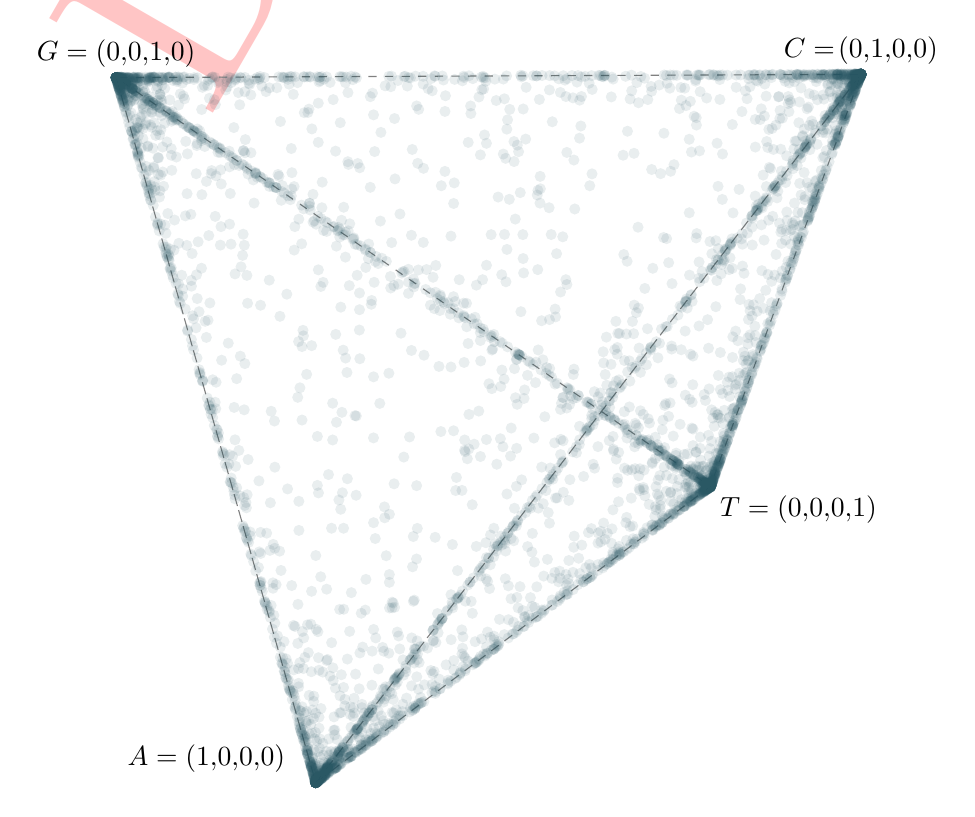
\begin{tikzpicture}[scale=10]


\begin{scope}[rotate around y=45,rotate around z=45]
 
% Draw the vertices of the tetrahedron

\coordinate (A) at (0, 0, 0);
\coordinate (C) at (1, 0, 0);
\coordinate (G) at (0.5, 0.866, 0);
\coordinate (T) at (0.5, 0.2887, 0.816);

%\foreach \p in {A,C,G,T}\fill[black] (\p) circle (0.02);

% Draw the edges of the cube
\draw[white!50!black, dashed]  (A) -- (C) -- (G) -- (A) -- (C) -- (T) -- (A) -- (T) -- (G) --  cycle;



    \pgfmathsetmacro{\alphaa}{0.1}       
       
\fill[color1,  opacity=\alphaa] (0.423,0.586,0.046) circle (.2pt);
         \fill[color1,  opacity=\alphaa] (0.984,0.027,0) circle (.2pt);
         \fill[color1,  opacity=\alphaa] (0.286,0.29,0.207) circle (.2pt);
         \fill[color1,  opacity=\alphaa] (0.842,0.106,0) circle (.2pt);
         \fill[color1,  opacity=\alphaa] (0.604,0.399,0.404) circle (.2pt);
         \fill[color1,  opacity=\alphaa] (0.093,0.02,0.057) circle (.2pt);
         \fill[color1,  opacity=\alphaa] (0,0,0) circle (.2pt);
         \fill[color1,  opacity=\alphaa] (0.231,0,0) circle (.2pt);
         \fill[color1,  opacity=\alphaa] (1,0,0) circle (.2pt);
         \fill[color1,  opacity=\alphaa] (0.36,0.556,0.003) circle (.2pt);
         \fill[color1,  opacity=\alphaa] (0.454,0.593,0.229) circle (.2pt);
         \fill[color1,  opacity=\alphaa] (0.506,0.85,0) circle (.2pt);
         \fill[color1,  opacity=\alphaa] (0.414,0.41,0.052) circle (.2pt);
         \fill[color1,  opacity=\alphaa] (0.533,0.269,0.762) circle (.2pt);
         \fill[color1,  opacity=\alphaa] (0.488,0.837,0) circle (.2pt);
         \fill[color1,  opacity=\alphaa] (0.001,0,0) circle (.2pt);
         \fill[color1,  opacity=\alphaa] (0.364,0.631,0) circle (.2pt);
         \fill[color1,  opacity=\alphaa] (0.495,0.836,0) circle (.2pt);
         \fill[color1,  opacity=\alphaa] (0.996,0.001,0) circle (.2pt);
         \fill[color1,  opacity=\alphaa] (0.999,0,0.001) circle (.2pt);
         \fill[color1,  opacity=\alphaa] (0.453,0.784,0) circle (.2pt);
         \fill[color1,  opacity=\alphaa] (0.405,0.235,0.66) circle (.2pt);
         \fill[color1,  opacity=\alphaa] (0.828,0.099,0.281) circle (.2pt);
         \fill[color1,  opacity=\alphaa] (0.648,0.186,0.526) circle (.2pt);
         \fill[color1,  opacity=\alphaa] (0.488,0.846,0) circle (.2pt);
         \fill[color1,  opacity=\alphaa] (0.47,0.438,0.499) circle (.2pt);
         \fill[color1,  opacity=\alphaa] (0.498,0.863,0) circle (.2pt);
         \fill[color1,  opacity=\alphaa] (0.006,0.01,0) circle (.2pt);
         \fill[color1,  opacity=\alphaa] (0.5,0.839,0.038) circle (.2pt);
         \fill[color1,  opacity=\alphaa] (0.605,0.051,0) circle (.2pt);
         \fill[color1,  opacity=\alphaa] (0.485,0.287,0.782) circle (.2pt);
         \fill[color1,  opacity=\alphaa] (0.516,0.502,0.418) circle (.2pt);
         \fill[color1,  opacity=\alphaa] (0.035,0.025,0.051) circle (.2pt);
         \fill[color1,  opacity=\alphaa] (0.5,0.289,0.816) circle (.2pt);
         \fill[color1,  opacity=\alphaa] (0.267,0.463,0) circle (.2pt);
         \fill[color1,  opacity=\alphaa] (0.5,0.289,0.816) circle (.2pt);
         \fill[color1,  opacity=\alphaa] (0.482,0.827,0) circle (.2pt);
         \fill[color1,  opacity=\alphaa] (0.5,0.298,0.804) circle (.2pt);
         \fill[color1,  opacity=\alphaa] (0.5,0.866,0) circle (.2pt);
         \fill[color1,  opacity=\alphaa] (0.5,0.289,0.816) circle (.2pt);
         \fill[color1,  opacity=\alphaa] (0.844,0.092,0.252) circle (.2pt);
         \fill[color1,  opacity=\alphaa] (0.476,0.583,0.341) circle (.2pt);
         \fill[color1,  opacity=\alphaa] (0.46,0.777,0.029) circle (.2pt);
         \fill[color1,  opacity=\alphaa] (0.996,0.007,0) circle (.2pt);
         \fill[color1,  opacity=\alphaa] (0.392,0.498,0.256) circle (.2pt);
         \fill[color1,  opacity=\alphaa] (0.977,0.013,0.038) circle (.2pt);
         \fill[color1,  opacity=\alphaa] (0.95,0.032,0.077) circle (.2pt);
         \fill[color1,  opacity=\alphaa] (0.436,0.611,0.002) circle (.2pt);
         \fill[color1,  opacity=\alphaa] (0.025,0.029,0.019) circle (.2pt);
         \fill[color1,  opacity=\alphaa] (0.952,0.028,0.079) circle (.2pt);
         \fill[color1,  opacity=\alphaa] (0.975,0.004,0.011) circle (.2pt);
         \fill[color1,  opacity=\alphaa] (0.006,0.002,0.006) circle (.2pt);
         \fill[color1,  opacity=\alphaa] (0.52,0.261,0.738) circle (.2pt);
         \fill[color1,  opacity=\alphaa] (0.319,0.184,0.521) circle (.2pt);
         \fill[color1,  opacity=\alphaa] (0.382,0.238,0.595) circle (.2pt);
         \fill[color1,  opacity=\alphaa] (0.207,0.357,0) circle (.2pt);
         \fill[color1,  opacity=\alphaa] (0.5,0.851,0.022) circle (.2pt);
         \fill[color1,  opacity=\alphaa] (0.575,0.22,0.616) circle (.2pt);
         \fill[color1,  opacity=\alphaa] (0.489,0.804,0.06) circle (.2pt);
         \fill[color1,  opacity=\alphaa] (0.968,0.006,0) circle (.2pt);
         \fill[color1,  opacity=\alphaa] (0.403,0,0) circle (.2pt);
         \fill[color1,  opacity=\alphaa] (0.008,0,0) circle (.2pt);
         \fill[color1,  opacity=\alphaa] (0.523,0.275,0.778) circle (.2pt);
         \fill[color1,  opacity=\alphaa] (0.5,0.474,0.554) circle (.2pt);
         \fill[color1,  opacity=\alphaa] (0.516,0.822,0.022) circle (.2pt);
         \fill[color1,  opacity=\alphaa] (0.021,0.001,0.003) circle (.2pt);
         \fill[color1,  opacity=\alphaa] (0.5,0.866,0) circle (.2pt);
         \fill[color1,  opacity=\alphaa] (0.339,0,0) circle (.2pt);
         \fill[color1,  opacity=\alphaa] (0.505,0.856,0.002) circle (.2pt);
         \fill[color1,  opacity=\alphaa] (0.002,0,0) circle (.2pt);
         \fill[color1,  opacity=\alphaa] (0.132,0.044,0.125) circle (.2pt);
         \fill[color1,  opacity=\alphaa] (0.508,0.851,0) circle (.2pt);
         \fill[color1,  opacity=\alphaa] (0,0,0) circle (.2pt);
         \fill[color1,  opacity=\alphaa] (0.831,0.29,0.003) circle (.2pt);
         \fill[color1,  opacity=\alphaa] (0,0,0) circle (.2pt);
         \fill[color1,  opacity=\alphaa] (0.502,0.301,0.793) circle (.2pt);
         \fill[color1,  opacity=\alphaa] (0.598,0.67,0.001) circle (.2pt);
         \fill[color1,  opacity=\alphaa] (0.5,0.846,0.028) circle (.2pt);
         \fill[color1,  opacity=\alphaa] (0.979,0.037,0) circle (.2pt);
         \fill[color1,  opacity=\alphaa] (0.548,0.78,0) circle (.2pt);
         \fill[color1,  opacity=\alphaa] (0.528,0.273,0.771) circle (.2pt);
         \fill[color1,  opacity=\alphaa] (0.445,0.769,0) circle (.2pt);
         \fill[color1,  opacity=\alphaa] (1,0,0) circle (.2pt);
         \fill[color1,  opacity=\alphaa] (0.461,0.264,0.748) circle (.2pt);
         \fill[color1,  opacity=\alphaa] (0.486,0.779,0.087) circle (.2pt);
         \fill[color1,  opacity=\alphaa] (0.074,0.018,0.034) circle (.2pt);
         \fill[color1,  opacity=\alphaa] (0.205,0.014,0.04) circle (.2pt);
         \fill[color1,  opacity=\alphaa] (0.501,0.288,0.815) circle (.2pt);
         \fill[color1,  opacity=\alphaa] (0.901,0.171,0) circle (.2pt);
         \fill[color1,  opacity=\alphaa] (0.5,0.305,0.793) circle (.2pt);
         \fill[color1,  opacity=\alphaa] (0.476,0.275,0.777) circle (.2pt);
         \fill[color1,  opacity=\alphaa] (0.563,0.749,0.011) circle (.2pt);
         \fill[color1,  opacity=\alphaa] (0.194,0.005,0.014) circle (.2pt);
         \fill[color1,  opacity=\alphaa] (0.5,0.289,0.816) circle (.2pt);
         \fill[color1,  opacity=\alphaa] (0.984,0,0) circle (.2pt);
         \fill[color1,  opacity=\alphaa] (0.97,0.016,0.013) circle (.2pt);
         \fill[color1,  opacity=\alphaa] (0.494,0.855,0) circle (.2pt);
         \fill[color1,  opacity=\alphaa] (0.497,0.287,0.811) circle (.2pt);
         \fill[color1,  opacity=\alphaa] (0.883,0.202,0) circle (.2pt);
         \fill[color1,  opacity=\alphaa] (0.305,0.055,0.001) circle (.2pt);
         \fill[color1,  opacity=\alphaa] (0.356,0.211,0.574) circle (.2pt);
         \fill[color1,  opacity=\alphaa] (0.02,0.035,0) circle (.2pt);
         \fill[color1,  opacity=\alphaa] (0.796,0.117,0.33) circle (.2pt);
         \fill[color1,  opacity=\alphaa] (0.391,0.161,0.43) circle (.2pt);
         \fill[color1,  opacity=\alphaa] (0.099,0.001,0) circle (.2pt);
         \fill[color1,  opacity=\alphaa] (0,0,0) circle (.2pt);
         \fill[color1,  opacity=\alphaa] (0.483,0.411,0.603) circle (.2pt);
         \fill[color1,  opacity=\alphaa] (0.5,0.289,0.816) circle (.2pt);
         \fill[color1,  opacity=\alphaa] (0.499,0.288,0.815) circle (.2pt);
         \fill[color1,  opacity=\alphaa] (0.499,0.864,0) circle (.2pt);
         \fill[color1,  opacity=\alphaa] (0.496,0.285,0.807) circle (.2pt);
         \fill[color1,  opacity=\alphaa] (0.493,0.852,0.002) circle (.2pt);
         \fill[color1,  opacity=\alphaa] (0.501,0.296,0.803) circle (.2pt);
         \fill[color1,  opacity=\alphaa] (0.155,0.26,0) circle (.2pt);
         \fill[color1,  opacity=\alphaa] (0.493,0.285,0.806) circle (.2pt);
         \fill[color1,  opacity=\alphaa] (0.581,0.14,0.377) circle (.2pt);
         \fill[color1,  opacity=\alphaa] (0.738,0,0) circle (.2pt);
         \fill[color1,  opacity=\alphaa] (0.655,0.199,0.563) circle (.2pt);
         \fill[color1,  opacity=\alphaa] (0.492,0.694,0.221) circle (.2pt);
         \fill[color1,  opacity=\alphaa] (0.502,0.86,0.004) circle (.2pt);
         \fill[color1,  opacity=\alphaa] (0.725,0.023,0.066) circle (.2pt);
         \fill[color1,  opacity=\alphaa] (0.029,0.049,0) circle (.2pt);
         \fill[color1,  opacity=\alphaa] (0.262,0,0) circle (.2pt);
         \fill[color1,  opacity=\alphaa] (0.382,0.368,0.414) circle (.2pt);
         \fill[color1,  opacity=\alphaa] (0.999,0.001,0.002) circle (.2pt);
         \fill[color1,  opacity=\alphaa] (0.5,0.313,0.783) circle (.2pt);
         \fill[color1,  opacity=\alphaa] (0.999,0,0) circle (.2pt);
         \fill[color1,  opacity=\alphaa] (0.496,0.858,0.001) circle (.2pt);
         \fill[color1,  opacity=\alphaa] (0.71,0.171,0.469) circle (.2pt);
         \fill[color1,  opacity=\alphaa] (0.025,0.014,0.041) circle (.2pt);
         \fill[color1,  opacity=\alphaa] (0.049,0,0) circle (.2pt);
         \fill[color1,  opacity=\alphaa] (0.439,0.15,0.424) circle (.2pt);
         \fill[color1,  opacity=\alphaa] (0.261,0.151,0.418) circle (.2pt);
         \fill[color1,  opacity=\alphaa] (0,0,0) circle (.2pt);
         \fill[color1,  opacity=\alphaa] (0.5,0.864,0.002) circle (.2pt);
         \fill[color1,  opacity=\alphaa] (0.347,0.427,0.242) circle (.2pt);
         \fill[color1,  opacity=\alphaa] (0.95,0.029,0.081) circle (.2pt);
         \fill[color1,  opacity=\alphaa] (1,0,0) circle (.2pt);
         \fill[color1,  opacity=\alphaa] (0.988,0.02,0) circle (.2pt);
         \fill[color1,  opacity=\alphaa] (0.784,0.124,0.35) circle (.2pt);
         \fill[color1,  opacity=\alphaa] (0.468,0.274,0.759) circle (.2pt);
         \fill[color1,  opacity=\alphaa] (0.286,0.093,0.263) circle (.2pt);
         \fill[color1,  opacity=\alphaa] (0.493,0.847,0.009) circle (.2pt);
         \fill[color1,  opacity=\alphaa] (0.927,0,0) circle (.2pt);
         \fill[color1,  opacity=\alphaa] (0.429,0,0) circle (.2pt);
         \fill[color1,  opacity=\alphaa] (0.916,0.047,0.133) circle (.2pt);
         \fill[color1,  opacity=\alphaa] (0.613,0,0.001) circle (.2pt);
         \fill[color1,  opacity=\alphaa] (0.5,0.327,0.763) circle (.2pt);
         \fill[color1,  opacity=\alphaa] (0.963,0.007,0) circle (.2pt);
         \fill[color1,  opacity=\alphaa] (0.534,0.268,0.759) circle (.2pt);
         \fill[color1,  opacity=\alphaa] (0.483,0.309,0.747) circle (.2pt);
         \fill[color1,  opacity=\alphaa] (0.499,0.865,0) circle (.2pt);
         \fill[color1,  opacity=\alphaa] (0.285,0.452,0.057) circle (.2pt);
         \fill[color1,  opacity=\alphaa] (0.848,0.088,0.247) circle (.2pt);
         \fill[color1,  opacity=\alphaa] (0.118,0.203,0.003) circle (.2pt);
         \fill[color1,  opacity=\alphaa] (1,0,0) circle (.2pt);
         \fill[color1,  opacity=\alphaa] (0.261,0.018,0.05) circle (.2pt);
         \fill[color1,  opacity=\alphaa] (0.5,0.866,0) circle (.2pt);
         \fill[color1,  opacity=\alphaa] (0.5,0.339,0.744) circle (.2pt);
         \fill[color1,  opacity=\alphaa] (0.066,0.113,0) circle (.2pt);
         \fill[color1,  opacity=\alphaa] (0.507,0.285,0.806) circle (.2pt);
         \fill[color1,  opacity=\alphaa] (0.023,0.004,0.01) circle (.2pt);
         \fill[color1,  opacity=\alphaa] (0.139,0.148,0) circle (.2pt);
         \fill[color1,  opacity=\alphaa] (0.507,0.332,0.74) circle (.2pt);
         \fill[color1,  opacity=\alphaa] (0.5,0.865,0.001) circle (.2pt);
         \fill[color1,  opacity=\alphaa] (0.5,0.301,0.799) circle (.2pt);
         \fill[color1,  opacity=\alphaa] (0.012,0.021,0) circle (.2pt);
         \fill[color1,  opacity=\alphaa] (0.459,0.767,0) circle (.2pt);
         \fill[color1,  opacity=\alphaa] (0.779,0.128,0.36) circle (.2pt);
         \fill[color1,  opacity=\alphaa] (0.5,0.699,0.236) circle (.2pt);
         \fill[color1,  opacity=\alphaa] (0.868,0.229,0) circle (.2pt);
         \fill[color1,  opacity=\alphaa] (0.004,0,0) circle (.2pt);
         \fill[color1,  opacity=\alphaa] (0.5,0.663,0.288) circle (.2pt);
         \fill[color1,  opacity=\alphaa] (0.496,0.507,0.498) circle (.2pt);
         \fill[color1,  opacity=\alphaa] (0.184,0.289,0.043) circle (.2pt);
         \fill[color1,  opacity=\alphaa] (0.5,0.863,0.004) circle (.2pt);
         \fill[color1,  opacity=\alphaa] (0.955,0.032,0.066) circle (.2pt);
         \fill[color1,  opacity=\alphaa] (0.484,0.838,0.002) circle (.2pt);
         \fill[color1,  opacity=\alphaa] (0.043,0.074,0) circle (.2pt);
         \fill[color1,  opacity=\alphaa] (0.501,0.31,0.784) circle (.2pt);
         \fill[color1,  opacity=\alphaa] (0.992,0.009,0) circle (.2pt);
         \fill[color1,  opacity=\alphaa] (0.491,0.851,0) circle (.2pt);
         \fill[color1,  opacity=\alphaa] (0.499,0.291,0.809) circle (.2pt);
         \fill[color1,  opacity=\alphaa] (0,0,0) circle (.2pt);
         \fill[color1,  opacity=\alphaa] (0.047,0.012,0.033) circle (.2pt);
         \fill[color1,  opacity=\alphaa] (0.961,0.067,0) circle (.2pt);
         \fill[color1,  opacity=\alphaa] (0.502,0.287,0.813) circle (.2pt);
         \fill[color1,  opacity=\alphaa] (0.499,0.288,0.814) circle (.2pt);
         \fill[color1,  opacity=\alphaa] (0.181,0.161,0) circle (.2pt);
         \fill[color1,  opacity=\alphaa] (0.455,0.783,0.001) circle (.2pt);
         \fill[color1,  opacity=\alphaa] (0.875,0,0) circle (.2pt);
         \fill[color1,  opacity=\alphaa] (0.505,0.304,0.782) circle (.2pt);
         \fill[color1,  opacity=\alphaa] (0.66,0.221,0.519) circle (.2pt);
         \fill[color1,  opacity=\alphaa] (0.564,0.252,0.712) circle (.2pt);
         \fill[color1,  opacity=\alphaa] (0.5,0.289,0.816) circle (.2pt);
         \fill[color1,  opacity=\alphaa] (0.5,0.289,0.816) circle (.2pt);
         \fill[color1,  opacity=\alphaa] (0.667,0.325,0.355) circle (.2pt);
         \fill[color1,  opacity=\alphaa] (1,0,0) circle (.2pt);
         \fill[color1,  opacity=\alphaa] (0.406,0.454,0.29) circle (.2pt);
         \fill[color1,  opacity=\alphaa] (0.55,0.776,0.004) circle (.2pt);
         \fill[color1,  opacity=\alphaa] (0.309,0.179,0.505) circle (.2pt);
         \fill[color1,  opacity=\alphaa] (0.5,0.861,0.007) circle (.2pt);
         \fill[color1,  opacity=\alphaa] (0.47,0.723,0.127) circle (.2pt);
         \fill[color1,  opacity=\alphaa] (0.061,0.03,0.083) circle (.2pt);
         \fill[color1,  opacity=\alphaa] (1,0,0) circle (.2pt);
         \fill[color1,  opacity=\alphaa] (0.5,0.288,0.816) circle (.2pt);
         \fill[color1,  opacity=\alphaa] (0.001,0,0) circle (.2pt);
         \fill[color1,  opacity=\alphaa] (0.5,0.865,0) circle (.2pt);
         \fill[color1,  opacity=\alphaa] (0.883,0.203,0) circle (.2pt);
         \fill[color1,  opacity=\alphaa] (0.224,0,0) circle (.2pt);
         \fill[color1,  opacity=\alphaa] (0.849,0.234,0) circle (.2pt);
         \fill[color1,  opacity=\alphaa] (0.484,0,0) circle (.2pt);
         \fill[color1,  opacity=\alphaa] (0.732,0.154,0.437) circle (.2pt);
         \fill[color1,  opacity=\alphaa] (0.998,0.001,0.004) circle (.2pt);
         \fill[color1,  opacity=\alphaa] (0.46,0.424,0.526) circle (.2pt);
         \fill[color1,  opacity=\alphaa] (0.524,0.825,0) circle (.2pt);
         \fill[color1,  opacity=\alphaa] (0.531,0.026,0.054) circle (.2pt);
         \fill[color1,  opacity=\alphaa] (0.022,0.001,0) circle (.2pt);
         \fill[color1,  opacity=\alphaa] (0.733,0.037,0.099) circle (.2pt);
         \fill[color1,  opacity=\alphaa] (0.5,0.339,0.745) circle (.2pt);
         \fill[color1,  opacity=\alphaa] (0.993,0.013,0) circle (.2pt);
         \fill[color1,  opacity=\alphaa] (0.5,0.857,0.013) circle (.2pt);
         \fill[color1,  opacity=\alphaa] (0.995,0.001,0.001) circle (.2pt);
         \fill[color1,  opacity=\alphaa] (0.075,0.103,0.039) circle (.2pt);
         \fill[color1,  opacity=\alphaa] (0.994,0.003,0.009) circle (.2pt);
         \fill[color1,  opacity=\alphaa] (0.855,0.021,0) circle (.2pt);
         \fill[color1,  opacity=\alphaa] (0.5,0.856,0.014) circle (.2pt);
         \fill[color1,  opacity=\alphaa] (0.995,0.003,0.008) circle (.2pt);
         \fill[color1,  opacity=\alphaa] (1,0,0) circle (.2pt);
         \fill[color1,  opacity=\alphaa] (0.002,0.001,0) circle (.2pt);
         \fill[color1,  opacity=\alphaa] (0.994,0,0.001) circle (.2pt);
         \fill[color1,  opacity=\alphaa] (0.493,0.281,0.794) circle (.2pt);
         \fill[color1,  opacity=\alphaa] (0.825,0.303,0) circle (.2pt);
         \fill[color1,  opacity=\alphaa] (0.501,0.859,0.008) circle (.2pt);
         \fill[color1,  opacity=\alphaa] (0.496,0.286,0.808) circle (.2pt);
         \fill[color1,  opacity=\alphaa] (0.497,0.283,0.799) circle (.2pt);
         \fill[color1,  opacity=\alphaa] (0.501,0.288,0.814) circle (.2pt);
         \fill[color1,  opacity=\alphaa] (0.502,0.298,0.798) circle (.2pt);
         \fill[color1,  opacity=\alphaa] (0.229,0.059,0.017) circle (.2pt);
         \fill[color1,  opacity=\alphaa] (0.5,0.858,0.011) circle (.2pt);
         \fill[color1,  opacity=\alphaa] (0.5,0.866,0) circle (.2pt);
         \fill[color1,  opacity=\alphaa] (0.17,0.06,0) circle (.2pt);
         \fill[color1,  opacity=\alphaa] (0.398,0.686,0.006) circle (.2pt);
         \fill[color1,  opacity=\alphaa] (0.949,0.071,0) circle (.2pt);
         \fill[color1,  opacity=\alphaa] (0.5,0.289,0.816) circle (.2pt);
         \fill[color1,  opacity=\alphaa] (0.976,0.03,0) circle (.2pt);
         \fill[color1,  opacity=\alphaa] (0.286,0.109,0.003) circle (.2pt);
         \fill[color1,  opacity=\alphaa] (0.002,0.001,0.002) circle (.2pt);
         \fill[color1,  opacity=\alphaa] (0.345,0.559,0) circle (.2pt);
         \fill[color1,  opacity=\alphaa] (0.456,0.633,0.219) circle (.2pt);
         \fill[color1,  opacity=\alphaa] (0.499,0.833,0.045) circle (.2pt);
         \fill[color1,  opacity=\alphaa] (0.01,0.005,0.002) circle (.2pt);
         \fill[color1,  opacity=\alphaa] (0.491,0.33,0.735) circle (.2pt);
         \fill[color1,  opacity=\alphaa] (0.554,0.752,0) circle (.2pt);
         \fill[color1,  opacity=\alphaa] (0.493,0.854,0) circle (.2pt);
         \fill[color1,  opacity=\alphaa] (0.999,0.001,0) circle (.2pt);
         \fill[color1,  opacity=\alphaa] (0.984,0.028,0) circle (.2pt);
         \fill[color1,  opacity=\alphaa] (0.999,0,0) circle (.2pt);
         \fill[color1,  opacity=\alphaa] (0.071,0.041,0.117) circle (.2pt);
         \fill[color1,  opacity=\alphaa] (0,0,0) circle (.2pt);
         \fill[color1,  opacity=\alphaa] (0.572,0.649,0.13) circle (.2pt);
         \fill[color1,  opacity=\alphaa] (0.406,0.235,0.662) circle (.2pt);
         \fill[color1,  opacity=\alphaa] (0.001,0.001,0.001) circle (.2pt);
         \fill[color1,  opacity=\alphaa] (0.998,0.001,0.003) circle (.2pt);
         \fill[color1,  opacity=\alphaa] (0.334,0,0) circle (.2pt);
         \fill[color1,  opacity=\alphaa] (0.989,0,0) circle (.2pt);
         \fill[color1,  opacity=\alphaa] (0.716,0.485,0.005) circle (.2pt);
         \fill[color1,  opacity=\alphaa] (0.002,0.004,0) circle (.2pt);
         \fill[color1,  opacity=\alphaa] (0.948,0.033,0.08) circle (.2pt);
         \fill[color1,  opacity=\alphaa] (0.996,0.002,0.007) circle (.2pt);
         \fill[color1,  opacity=\alphaa] (0.03,0.048,0) circle (.2pt);
         \fill[color1,  opacity=\alphaa] (0.503,0.335,0.744) circle (.2pt);
         \fill[color1,  opacity=\alphaa] (0.241,0.001,0) circle (.2pt);
         \fill[color1,  opacity=\alphaa] (0.063,0,0) circle (.2pt);
         \fill[color1,  opacity=\alphaa] (0.5,0.289,0.816) circle (.2pt);
         \fill[color1,  opacity=\alphaa] (0,0,0) circle (.2pt);
         \fill[color1,  opacity=\alphaa] (0.026,0,0) circle (.2pt);
         \fill[color1,  opacity=\alphaa] (0.021,0.037,0) circle (.2pt);
         \fill[color1,  opacity=\alphaa] (0.511,0.836,0.013) circle (.2pt);
         \fill[color1,  opacity=\alphaa] (0.953,0.027,0.076) circle (.2pt);
         \fill[color1,  opacity=\alphaa] (0.013,0,0) circle (.2pt);
         \fill[color1,  opacity=\alphaa] (0.452,0.288,0.7) circle (.2pt);
         \fill[color1,  opacity=\alphaa] (0.004,0.002,0.006) circle (.2pt);
         \fill[color1,  opacity=\alphaa] (0.455,0.055,0) circle (.2pt);
         \fill[color1,  opacity=\alphaa] (0.775,0.13,0.367) circle (.2pt);
         \fill[color1,  opacity=\alphaa] (0.5,0.289,0.816) circle (.2pt);
         \fill[color1,  opacity=\alphaa] (0.841,0,0) circle (.2pt);
         \fill[color1,  opacity=\alphaa] (0.732,0.004,0.009) circle (.2pt);
         \fill[color1,  opacity=\alphaa] (0.488,0.282,0.797) circle (.2pt);
         \fill[color1,  opacity=\alphaa] (0.003,0.005,0) circle (.2pt);
         \fill[color1,  opacity=\alphaa] (0.5,0.866,0.001) circle (.2pt);
         \fill[color1,  opacity=\alphaa] (0.513,0.281,0.796) circle (.2pt);
         \fill[color1,  opacity=\alphaa] (0.497,0.31,0.778) circle (.2pt);
         \fill[color1,  opacity=\alphaa] (0.83,0.289,0.007) circle (.2pt);
         \fill[color1,  opacity=\alphaa] (0.501,0.288,0.814) circle (.2pt);
         \fill[color1,  opacity=\alphaa] (0.5,0.29,0.815) circle (.2pt);
         \fill[color1,  opacity=\alphaa] (0.971,0.02,0.041) circle (.2pt);
         \fill[color1,  opacity=\alphaa] (0,0,0) circle (.2pt);
         \fill[color1,  opacity=\alphaa] (0.513,0.82,0.034) circle (.2pt);
         \fill[color1,  opacity=\alphaa] (0.518,0.67,0.234) circle (.2pt);
         \fill[color1,  opacity=\alphaa] (0.989,0.006,0.018) circle (.2pt);
         \fill[color1,  opacity=\alphaa] (1,0,0) circle (.2pt);
         \fill[color1,  opacity=\alphaa] (0.5,0.854,0.017) circle (.2pt);
         \fill[color1,  opacity=\alphaa] (0.501,0.797,0.059) circle (.2pt);
         \fill[color1,  opacity=\alphaa] (0.783,0.139,0.335) circle (.2pt);
         \fill[color1,  opacity=\alphaa] (0.194,0.135,0.01) circle (.2pt);
         \fill[color1,  opacity=\alphaa] (0.504,0.86,0) circle (.2pt);
         \fill[color1,  opacity=\alphaa] (0.915,0.049,0.139) circle (.2pt);
         \fill[color1,  opacity=\alphaa] (0.006,0.003,0.01) circle (.2pt);
         \fill[color1,  opacity=\alphaa] (0.5,0.393,0.669) circle (.2pt);
         \fill[color1,  opacity=\alphaa] (0.001,0,0.001) circle (.2pt);
         \fill[color1,  opacity=\alphaa] (0.916,0.089,0.065) circle (.2pt);
         \fill[color1,  opacity=\alphaa] (0.003,0,0) circle (.2pt);
         \fill[color1,  opacity=\alphaa] (0.552,0.216,0.612) circle (.2pt);
         \fill[color1,  opacity=\alphaa] (0.987,0.023,0) circle (.2pt);
         \fill[color1,  opacity=\alphaa] (0.883,0,0) circle (.2pt);
         \fill[color1,  opacity=\alphaa] (0.362,0,0) circle (.2pt);
         \fill[color1,  opacity=\alphaa] (0.952,0.003,0.003) circle (.2pt);
         \fill[color1,  opacity=\alphaa] (0.091,0.151,0.009) circle (.2pt);
         \fill[color1,  opacity=\alphaa] (0.426,0.733,0.007) circle (.2pt);
         \fill[color1,  opacity=\alphaa] (0.5,0.861,0.007) circle (.2pt);
         \fill[color1,  opacity=\alphaa] (0.5,0.289,0.816) circle (.2pt);
         \fill[color1,  opacity=\alphaa] (0.62,0.658,0) circle (.2pt);
         \fill[color1,  opacity=\alphaa] (0.785,0.341,0.044) circle (.2pt);
         \fill[color1,  opacity=\alphaa] (0.004,0.007,0) circle (.2pt);
         \fill[color1,  opacity=\alphaa] (0.702,0.185,0.416) circle (.2pt);
         \fill[color1,  opacity=\alphaa] (0.071,0.041,0.116) circle (.2pt);
         \fill[color1,  opacity=\alphaa] (0.498,0.311,0.781) circle (.2pt);
         \fill[color1,  opacity=\alphaa] (0.499,0.86,0.006) circle (.2pt);
         \fill[color1,  opacity=\alphaa] (0.508,0.85,0) circle (.2pt);
         \fill[color1,  opacity=\alphaa] (0.006,0,0) circle (.2pt);
         \fill[color1,  opacity=\alphaa] (0.523,0.826,0) circle (.2pt);
         \fill[color1,  opacity=\alphaa] (0.001,0,0) circle (.2pt);
         \fill[color1,  opacity=\alphaa] (0.49,0.087,0.243) circle (.2pt);
         \fill[color1,  opacity=\alphaa] (0.5,0.857,0.013) circle (.2pt);
         \fill[color1,  opacity=\alphaa] (0.5,0.771,0.134) circle (.2pt);
         \fill[color1,  opacity=\alphaa] (0.444,0.365,0.572) circle (.2pt);
         \fill[color1,  opacity=\alphaa] (0.313,0.175,0.494) circle (.2pt);
         \fill[color1,  opacity=\alphaa] (0.497,0.287,0.812) circle (.2pt);
         \fill[color1,  opacity=\alphaa] (0.167,0.096,0.273) circle (.2pt);
         \fill[color1,  opacity=\alphaa] (0.5,0.528,0.477) circle (.2pt);
         \fill[color1,  opacity=\alphaa] (0.473,0.791,0.039) circle (.2pt);
         \fill[color1,  opacity=\alphaa] (0.892,0.187,0) circle (.2pt);
         \fill[color1,  opacity=\alphaa] (0.187,0.003,0) circle (.2pt);
         \fill[color1,  opacity=\alphaa] (0.497,0.857,0) circle (.2pt);
         \fill[color1,  opacity=\alphaa] (1,0,0) circle (.2pt);
         \fill[color1,  opacity=\alphaa] (0.031,0.018,0.051) circle (.2pt);
         \fill[color1,  opacity=\alphaa] (0.495,0.857,0) circle (.2pt);
         \fill[color1,  opacity=\alphaa] (0.807,0.3,0) circle (.2pt);
         \fill[color1,  opacity=\alphaa] (0.226,0.131,0.37) circle (.2pt);
         \fill[color1,  opacity=\alphaa] (0.984,0,0) circle (.2pt);
         \fill[color1,  opacity=\alphaa] (0.498,0.288,0.813) circle (.2pt);
         \fill[color1,  opacity=\alphaa] (0.011,0.019,0) circle (.2pt);
         \fill[color1,  opacity=\alphaa] (0.5,0.289,0.816) circle (.2pt);
         \fill[color1,  opacity=\alphaa] (0.936,0.11,0) circle (.2pt);
         \fill[color1,  opacity=\alphaa] (0.491,0.283,0.801) circle (.2pt);
         \fill[color1,  opacity=\alphaa] (0.419,0.242,0.675) circle (.2pt);
         \fill[color1,  opacity=\alphaa] (0.538,0.267,0.754) circle (.2pt);
         \fill[color1,  opacity=\alphaa] (0.501,0.288,0.814) circle (.2pt);
         \fill[color1,  opacity=\alphaa] (0.5,0.355,0.722) circle (.2pt);
         \fill[color1,  opacity=\alphaa] (0,0.001,0) circle (.2pt);
         \fill[color1,  opacity=\alphaa] (0.286,0.165,0.467) circle (.2pt);
         \fill[color1,  opacity=\alphaa] (0.5,0.67,0.277) circle (.2pt);
         \fill[color1,  opacity=\alphaa] (0.03,0,0) circle (.2pt);
         \fill[color1,  opacity=\alphaa] (0.072,0.035,0.099) circle (.2pt);
         \fill[color1,  opacity=\alphaa] (0.491,0.283,0.8) circle (.2pt);
         \fill[color1,  opacity=\alphaa] (0.113,0.146,0) circle (.2pt);
         \fill[color1,  opacity=\alphaa] (0.5,0.445,0.594) circle (.2pt);
         \fill[color1,  opacity=\alphaa] (0.246,0.426,0) circle (.2pt);
         \fill[color1,  opacity=\alphaa] (0.528,0.219,0.618) circle (.2pt);
         \fill[color1,  opacity=\alphaa] (0.985,0.012,0.021) circle (.2pt);
         \fill[color1,  opacity=\alphaa] (0.503,0.291,0.803) circle (.2pt);
         \fill[color1,  opacity=\alphaa] (0.5,0.85,0.023) circle (.2pt);
         \fill[color1,  opacity=\alphaa] (0.201,0.339,0.012) circle (.2pt);
         \fill[color1,  opacity=\alphaa] (0.5,0.766,0.141) circle (.2pt);
         \fill[color1,  opacity=\alphaa] (0.069,0.075,0.063) circle (.2pt);
         \fill[color1,  opacity=\alphaa] (0.999,0,0.001) circle (.2pt);
         \fill[color1,  opacity=\alphaa] (0.722,0.161,0.454) circle (.2pt);
         \fill[color1,  opacity=\alphaa] (0.501,0.3,0.798) circle (.2pt);
         \fill[color1,  opacity=\alphaa] (0.264,0.153,0.432) circle (.2pt);
         \fill[color1,  opacity=\alphaa] (0.077,0,0) circle (.2pt);
         \fill[color1,  opacity=\alphaa] (0.812,0.088,0.239) circle (.2pt);
         \fill[color1,  opacity=\alphaa] (0.565,0.488,0.376) circle (.2pt);
         \fill[color1,  opacity=\alphaa] (0.968,0.055,0) circle (.2pt);
         \fill[color1,  opacity=\alphaa] (0,0,0.001) circle (.2pt);
         \fill[color1,  opacity=\alphaa] (0.526,0.822,0) circle (.2pt);
         \fill[color1,  opacity=\alphaa] (0.467,0.27,0.762) circle (.2pt);
         \fill[color1,  opacity=\alphaa] (0.025,0,0) circle (.2pt);
         \fill[color1,  opacity=\alphaa] (0.5,0.325,0.765) circle (.2pt);
         \fill[color1,  opacity=\alphaa] (0.257,0.301,0.143) circle (.2pt);
         \fill[color1,  opacity=\alphaa] (0.009,0,0.001) circle (.2pt);
         \fill[color1,  opacity=\alphaa] (0.686,0.53,0.019) circle (.2pt);
         \fill[color1,  opacity=\alphaa] (0.5,0.866,0) circle (.2pt);
         \fill[color1,  opacity=\alphaa] (0.735,0.191,0.38) circle (.2pt);
         \fill[color1,  opacity=\alphaa] (0.499,0.864,0) circle (.2pt);
         \fill[color1,  opacity=\alphaa] (0,0,0) circle (.2pt);
         \fill[color1,  opacity=\alphaa] (0.971,0.051,0) circle (.2pt);
         \fill[color1,  opacity=\alphaa] (0.934,0.047,0) circle (.2pt);
         \fill[color1,  opacity=\alphaa] (0.5,0.501,0.517) circle (.2pt);
         \fill[color1,  opacity=\alphaa] (0.125,0.189,0.037) circle (.2pt);
         \fill[color1,  opacity=\alphaa] (0.5,0.861,0.006) circle (.2pt);
         \fill[color1,  opacity=\alphaa] (0.5,0.788,0.109) circle (.2pt);
         \fill[color1,  opacity=\alphaa] (0.003,0.003,0.002) circle (.2pt);
         \fill[color1,  opacity=\alphaa] (0.501,0.865,0) circle (.2pt);
         \fill[color1,  opacity=\alphaa] (0.931,0.072,0.012) circle (.2pt);
         \fill[color1,  opacity=\alphaa] (0.5,0.865,0) circle (.2pt);
         \fill[color1,  opacity=\alphaa] (1,0.001,0) circle (.2pt);
         \fill[color1,  opacity=\alphaa] (0.004,0.007,0) circle (.2pt);
         \fill[color1,  opacity=\alphaa] (0.237,0.395,0) circle (.2pt);
         \fill[color1,  opacity=\alphaa] (0.499,0.294,0.807) circle (.2pt);
         \fill[color1,  opacity=\alphaa] (0.516,0.28,0.791) circle (.2pt);
         \fill[color1,  opacity=\alphaa] (0.461,0.172,0.486) circle (.2pt);
         \fill[color1,  opacity=\alphaa] (0.454,0.262,0.741) circle (.2pt);
         \fill[color1,  opacity=\alphaa] (0.013,0,0) circle (.2pt);
         \fill[color1,  opacity=\alphaa] (0.409,0.238,0.665) circle (.2pt);
         \fill[color1,  opacity=\alphaa] (0.5,0.866,0) circle (.2pt);
         \fill[color1,  opacity=\alphaa] (0.485,0.363,0.674) circle (.2pt);
         \fill[color1,  opacity=\alphaa] (0.489,0.417,0.608) circle (.2pt);
         \fill[color1,  opacity=\alphaa] (1,0,0) circle (.2pt);
         \fill[color1,  opacity=\alphaa] (0.001,0.001,0) circle (.2pt);
         \fill[color1,  opacity=\alphaa] (0.497,0.287,0.812) circle (.2pt);
         \fill[color1,  opacity=\alphaa] (0.037,0.005,0.014) circle (.2pt);
         \fill[color1,  opacity=\alphaa] (0.85,0.084,0.237) circle (.2pt);
         \fill[color1,  opacity=\alphaa] (0.46,0.537,0.286) circle (.2pt);
         \fill[color1,  opacity=\alphaa] (0.5,0.289,0.816) circle (.2pt);
         \fill[color1,  opacity=\alphaa] (0.5,0.289,0.816) circle (.2pt);
         \fill[color1,  opacity=\alphaa] (0.488,0.843,0.003) circle (.2pt);
         \fill[color1,  opacity=\alphaa] (0.482,0.278,0.783) circle (.2pt);
         \fill[color1,  opacity=\alphaa] (0.54,0.318,0.677) circle (.2pt);
         \fill[color1,  opacity=\alphaa] (0.5,0.289,0.816) circle (.2pt);
         \fill[color1,  opacity=\alphaa] (0.491,0.808,0) circle (.2pt);
         \fill[color1,  opacity=\alphaa] (0.727,0,0) circle (.2pt);
         \fill[color1,  opacity=\alphaa] (0,0,0) circle (.2pt);
         \fill[color1,  opacity=\alphaa] (0.699,0.174,0.491) circle (.2pt);
         \fill[color1,  opacity=\alphaa] (0,0,0) circle (.2pt);
         \fill[color1,  opacity=\alphaa] (0.5,0.865,0.001) circle (.2pt);
         \fill[color1,  opacity=\alphaa] (0.996,0.006,0.001) circle (.2pt);
         \fill[color1,  opacity=\alphaa] (0.901,0.172,0) circle (.2pt);
         \fill[color1,  opacity=\alphaa] (0.466,0.64,0.236) circle (.2pt);
         \fill[color1,  opacity=\alphaa] (0.062,0.034,0.094) circle (.2pt);
         \fill[color1,  opacity=\alphaa] (0.986,0.023,0) circle (.2pt);
         \fill[color1,  opacity=\alphaa] (0.997,0.002,0.005) circle (.2pt);
         \fill[color1,  opacity=\alphaa] (0.499,0.288,0.814) circle (.2pt);
         \fill[color1,  opacity=\alphaa] (0.963,0,0) circle (.2pt);
         \fill[color1,  opacity=\alphaa] (0,0,0) circle (.2pt);
         \fill[color1,  opacity=\alphaa] (0.354,0.339,0.387) circle (.2pt);
         \fill[color1,  opacity=\alphaa] (0.471,0.372,0.628) circle (.2pt);
         \fill[color1,  opacity=\alphaa] (0.971,0.017,0.046) circle (.2pt);
         \fill[color1,  opacity=\alphaa] (0.49,0.281,0.795) circle (.2pt);
         \fill[color1,  opacity=\alphaa] (0.583,0.722,0.001) circle (.2pt);
         \fill[color1,  opacity=\alphaa] (0.487,0.844,0) circle (.2pt);
         \fill[color1,  opacity=\alphaa] (0.129,0.217,0.01) circle (.2pt);
         \fill[color1,  opacity=\alphaa] (0.998,0,0) circle (.2pt);
         \fill[color1,  opacity=\alphaa] (0.504,0.86,0) circle (.2pt);
         \fill[color1,  opacity=\alphaa] (0,0,0) circle (.2pt);
         \fill[color1,  opacity=\alphaa] (0.5,0.289,0.816) circle (.2pt);
         \fill[color1,  opacity=\alphaa] (0.896,0.002,0.005) circle (.2pt);
         \fill[color1,  opacity=\alphaa] (0.961,0.066,0.002) circle (.2pt);
         \fill[color1,  opacity=\alphaa] (0.554,0.313,0.651) circle (.2pt);
         \fill[color1,  opacity=\alphaa] (0.502,0.861,0) circle (.2pt);
         \fill[color1,  opacity=\alphaa] (0.587,0.278,0.609) circle (.2pt);
         \fill[color1,  opacity=\alphaa] (0.487,0.819,0.033) circle (.2pt);
         \fill[color1,  opacity=\alphaa] (0.457,0.791,0) circle (.2pt);
         \fill[color1,  opacity=\alphaa] (0.5,0.425,0.623) circle (.2pt);
         \fill[color1,  opacity=\alphaa] (0.426,0.235,0.663) circle (.2pt);
         \fill[color1,  opacity=\alphaa] (0.511,0,0) circle (.2pt);
         \fill[color1,  opacity=\alphaa] (0.023,0,0) circle (.2pt);
         \fill[color1,  opacity=\alphaa] (0.518,0.829,0.009) circle (.2pt);
         \fill[color1,  opacity=\alphaa] (0.877,0.002,0) circle (.2pt);
         \fill[color1,  opacity=\alphaa] (0.604,0.228,0.646) circle (.2pt);
         \fill[color1,  opacity=\alphaa] (0.027,0.042,0) circle (.2pt);
         \fill[color1,  opacity=\alphaa] (0.976,0.039,0) circle (.2pt);
         \fill[color1,  opacity=\alphaa] (0.497,0.291,0.806) circle (.2pt);
         \fill[color1,  opacity=\alphaa] (0.496,0.571,0.406) circle (.2pt);
         \fill[color1,  opacity=\alphaa] (0.558,0.371,0.385) circle (.2pt);
         \fill[color1,  opacity=\alphaa] (0.5,0.35,0.729) circle (.2pt);
         \fill[color1,  opacity=\alphaa] (0.268,0.265,0) circle (.2pt);
         \fill[color1,  opacity=\alphaa] (0.015,0.025,0) circle (.2pt);
         \fill[color1,  opacity=\alphaa] (0.487,0.449,0.558) circle (.2pt);
         \fill[color1,  opacity=\alphaa] (1,0,0) circle (.2pt);
         \fill[color1,  opacity=\alphaa] (0.989,0.006,0.017) circle (.2pt);
         \fill[color1,  opacity=\alphaa] (0.442,0.489,0.391) circle (.2pt);
         \fill[color1,  opacity=\alphaa] (0.508,0.85,0.003) circle (.2pt);
         \fill[color1,  opacity=\alphaa] (0.124,0.024,0.067) circle (.2pt);
         \fill[color1,  opacity=\alphaa] (0.121,0,0) circle (.2pt);
         \fill[color1,  opacity=\alphaa] (0.501,0.289,0.815) circle (.2pt);
         \fill[color1,  opacity=\alphaa] (0.496,0.778,0.115) circle (.2pt);
         \fill[color1,  opacity=\alphaa] (0,0,0) circle (.2pt);
         \fill[color1,  opacity=\alphaa] (0.047,0.064,0) circle (.2pt);
         \fill[color1,  opacity=\alphaa] (0.919,0.14,0) circle (.2pt);
         \fill[color1,  opacity=\alphaa] (0.925,0.129,0) circle (.2pt);
         \fill[color1,  opacity=\alphaa] (0.536,0.805,0) circle (.2pt);
         \fill[color1,  opacity=\alphaa] (0.996,0,0) circle (.2pt);
         \fill[color1,  opacity=\alphaa] (0.517,0.391,0.63) circle (.2pt);
         \fill[color1,  opacity=\alphaa] (0.459,0.267,0.747) circle (.2pt);
         \fill[color1,  opacity=\alphaa] (0.673,0.124,0.352) circle (.2pt);
         \fill[color1,  opacity=\alphaa] (0.036,0.062,0) circle (.2pt);
         \fill[color1,  opacity=\alphaa] (0.5,0.289,0.816) circle (.2pt);
         \fill[color1,  opacity=\alphaa] (0.184,0.103,0.293) circle (.2pt);
         \fill[color1,  opacity=\alphaa] (0.508,0.298,0.785) circle (.2pt);
         \fill[color1,  opacity=\alphaa] (0.5,0.289,0.816) circle (.2pt);
         \fill[color1,  opacity=\alphaa] (0.5,0.866,0) circle (.2pt);
         \fill[color1,  opacity=\alphaa] (0.732,0.412,0.057) circle (.2pt);
         \fill[color1,  opacity=\alphaa] (0.953,0.018,0.05) circle (.2pt);
         \fill[color1,  opacity=\alphaa] (0.467,0.776,0.045) circle (.2pt);
         \fill[color1,  opacity=\alphaa] (0.281,0.306,0.255) circle (.2pt);
         \fill[color1,  opacity=\alphaa] (0.905,0.134,0) circle (.2pt);
         \fill[color1,  opacity=\alphaa] (0,0,0) circle (.2pt);
         \fill[color1,  opacity=\alphaa] (0.974,0.044,0.001) circle (.2pt);
         \fill[color1,  opacity=\alphaa] (0.5,0.427,0.621) circle (.2pt);
         \fill[color1,  opacity=\alphaa] (0.577,0.517,0) circle (.2pt);
         \fill[color1,  opacity=\alphaa] (0.491,0.587,0.371) circle (.2pt);
         \fill[color1,  opacity=\alphaa] (0.737,0.456,0) circle (.2pt);
         \fill[color1,  opacity=\alphaa] (0.5,0.289,0.816) circle (.2pt);
         \fill[color1,  opacity=\alphaa] (0.96,0.066,0) circle (.2pt);
         \fill[color1,  opacity=\alphaa] (0.901,0,0) circle (.2pt);
         \fill[color1,  opacity=\alphaa] (0.5,0.862,0.006) circle (.2pt);
         \fill[color1,  opacity=\alphaa] (0.023,0.039,0) circle (.2pt);
         \fill[color1,  opacity=\alphaa] (0.081,0.075,0.091) circle (.2pt);
         \fill[color1,  opacity=\alphaa] (0.719,0.162,0.458) circle (.2pt);
         \fill[color1,  opacity=\alphaa] (0.5,0.289,0.816) circle (.2pt);
         \fill[color1,  opacity=\alphaa] (0.034,0.059,0) circle (.2pt);
         \fill[color1,  opacity=\alphaa] (0.753,0.143,0.404) circle (.2pt);
         \fill[color1,  opacity=\alphaa] (0.483,0.837,0) circle (.2pt);
         \fill[color1,  opacity=\alphaa] (0.042,0.049,0) circle (.2pt);
         \fill[color1,  opacity=\alphaa] (0.968,0.054,0.001) circle (.2pt);
         \fill[color1,  opacity=\alphaa] (0.153,0.084,0.236) circle (.2pt);
         \fill[color1,  opacity=\alphaa] (1,0,0) circle (.2pt);
         \fill[color1,  opacity=\alphaa] (0.499,0.289,0.815) circle (.2pt);
         \fill[color1,  opacity=\alphaa] (0.002,0.002,0) circle (.2pt);
         \fill[color1,  opacity=\alphaa] (0.5,0.289,0.816) circle (.2pt);
         \fill[color1,  opacity=\alphaa] (0.5,0.619,0.349) circle (.2pt);
         \fill[color1,  opacity=\alphaa] (0.499,0.811,0.077) circle (.2pt);
         \fill[color1,  opacity=\alphaa] (1,0,0) circle (.2pt);
         \fill[color1,  opacity=\alphaa] (0.109,0.104,0.119) circle (.2pt);
         \fill[color1,  opacity=\alphaa] (0.484,0.838,0) circle (.2pt);
         \fill[color1,  opacity=\alphaa] (0.216,0.124,0) circle (.2pt);
         \fill[color1,  opacity=\alphaa] (0.017,0,0) circle (.2pt);
         \fill[color1,  opacity=\alphaa] (0.919,0.003,0) circle (.2pt);
         \fill[color1,  opacity=\alphaa] (0.637,0.625,0.005) circle (.2pt);
         \fill[color1,  opacity=\alphaa] (0.5,0.837,0.041) circle (.2pt);
         \fill[color1,  opacity=\alphaa] (0.524,0.819,0.009) circle (.2pt);
         \fill[color1,  opacity=\alphaa] (1,0,0) circle (.2pt);
         \fill[color1,  opacity=\alphaa] (0.96,0.031,0.053) circle (.2pt);
         \fill[color1,  opacity=\alphaa] (0.109,0.189,0.001) circle (.2pt);
         \fill[color1,  opacity=\alphaa] (0.818,0.209,0.151) circle (.2pt);
         \fill[color1,  opacity=\alphaa] (0.021,0.015,0.031) circle (.2pt);
         \fill[color1,  opacity=\alphaa] (0.5,0.796,0.099) circle (.2pt);
         \fill[color1,  opacity=\alphaa] (0.319,0.244,0.435) circle (.2pt);
         \fill[color1,  opacity=\alphaa] (0.843,0,0) circle (.2pt);
         \fill[color1,  opacity=\alphaa] (0.501,0.288,0.815) circle (.2pt);
         \fill[color1,  opacity=\alphaa] (0.973,0.016,0.045) circle (.2pt);
         \fill[color1,  opacity=\alphaa] (0.796,0.197,0.221) circle (.2pt);
         \fill[color1,  opacity=\alphaa] (0.502,0.862,0) circle (.2pt);
         \fill[color1,  opacity=\alphaa] (0.02,0.012,0.033) circle (.2pt);
         \fill[color1,  opacity=\alphaa] (0.175,0.018,0.052) circle (.2pt);
         \fill[color1,  opacity=\alphaa] (0.495,0.856,0) circle (.2pt);
         \fill[color1,  opacity=\alphaa] (0.992,0.004,0.012) circle (.2pt);
         \fill[color1,  opacity=\alphaa] (0.502,0.862,0) circle (.2pt);
         \fill[color1,  opacity=\alphaa] (0.261,0,0) circle (.2pt);
         \fill[color1,  opacity=\alphaa] (0.953,0.081,0) circle (.2pt);
         \fill[color1,  opacity=\alphaa] (0.929,0.123,0) circle (.2pt);
         \fill[color1,  opacity=\alphaa] (0.568,0.266,0.679) circle (.2pt);
         \fill[color1,  opacity=\alphaa] (0.976,0.014,0.039) circle (.2pt);
         \fill[color1,  opacity=\alphaa] (0.514,0.288,0.783) circle (.2pt);
         \fill[color1,  opacity=\alphaa] (0.5,0.289,0.816) circle (.2pt);
         \fill[color1,  opacity=\alphaa] (0.897,0.046,0.13) circle (.2pt);
         \fill[color1,  opacity=\alphaa] (0.508,0.284,0.803) circle (.2pt);
         \fill[color1,  opacity=\alphaa] (0.501,0.864,0) circle (.2pt);
         \fill[color1,  opacity=\alphaa] (0.5,0.866,0) circle (.2pt);
         \fill[color1,  opacity=\alphaa] (0.622,0.452,0.044) circle (.2pt);
         \fill[color1,  opacity=\alphaa] (0.501,0.73,0.189) circle (.2pt);
         \fill[color1,  opacity=\alphaa] (0.39,0.314,0.326) circle (.2pt);
         \fill[color1,  opacity=\alphaa] (0.512,0.841,0) circle (.2pt);
         \fill[color1,  opacity=\alphaa] (0.388,0.425,0.047) circle (.2pt);
         \fill[color1,  opacity=\alphaa] (0.637,0.21,0.593) circle (.2pt);
         \fill[color1,  opacity=\alphaa] (0.727,0.21,0.367) circle (.2pt);
         \fill[color1,  opacity=\alphaa] (0.51,0.845,0) circle (.2pt);
         \fill[color1,  opacity=\alphaa] (0.5,0.866,0) circle (.2pt);
         \fill[color1,  opacity=\alphaa] (0.86,0.081,0.229) circle (.2pt);
         \fill[color1,  opacity=\alphaa] (0.5,0.324,0.766) circle (.2pt);
         \fill[color1,  opacity=\alphaa] (0.31,0.536,0) circle (.2pt);
         \fill[color1,  opacity=\alphaa] (0.608,0.333,0.487) circle (.2pt);
         \fill[color1,  opacity=\alphaa] (0.228,0,0) circle (.2pt);
         \fill[color1,  opacity=\alphaa] (0.498,0.857,0.007) circle (.2pt);
         \fill[color1,  opacity=\alphaa] (0.515,0.568,0.384) circle (.2pt);
         \fill[color1,  opacity=\alphaa] (0.542,0.764,0.043) circle (.2pt);
         \fill[color1,  opacity=\alphaa] (0.504,0.83,0.034) circle (.2pt);
         \fill[color1,  opacity=\alphaa] (0.011,0.01,0.012) circle (.2pt);
         \fill[color1,  opacity=\alphaa] (0.002,0.001,0.003) circle (.2pt);
         \fill[color1,  opacity=\alphaa] (0.898,0,0) circle (.2pt);
         \fill[color1,  opacity=\alphaa] (0.114,0.109,0) circle (.2pt);
         \fill[color1,  opacity=\alphaa] (0.603,0.646,0.003) circle (.2pt);
         \fill[color1,  opacity=\alphaa] (0.498,0.681,0.256) circle (.2pt);
         \fill[color1,  opacity=\alphaa] (0.499,0.864,0) circle (.2pt);
         \fill[color1,  opacity=\alphaa] (0.172,0.297,0) circle (.2pt);
         \fill[color1,  opacity=\alphaa] (0.995,0,0) circle (.2pt);
         \fill[color1,  opacity=\alphaa] (0.4,0.032,0) circle (.2pt);
         \fill[color1,  opacity=\alphaa] (0.853,0.106,0.187) circle (.2pt);
         \fill[color1,  opacity=\alphaa] (0.5,0.289,0.816) circle (.2pt);
         \fill[color1,  opacity=\alphaa] (0.616,0.657,0.012) circle (.2pt);
         \fill[color1,  opacity=\alphaa] (0.997,0.002,0.002) circle (.2pt);
         \fill[color1,  opacity=\alphaa] (0.011,0.003,0) circle (.2pt);
         \fill[color1,  opacity=\alphaa] (0.728,0.461,0.003) circle (.2pt);
         \fill[color1,  opacity=\alphaa] (0.994,0.011,0) circle (.2pt);
         \fill[color1,  opacity=\alphaa] (0.543,0.265,0.745) circle (.2pt);
         \fill[color1,  opacity=\alphaa] (0.448,0.47,0.43) circle (.2pt);
         \fill[color1,  opacity=\alphaa] (0.996,0.002,0.007) circle (.2pt);
         \fill[color1,  opacity=\alphaa] (0.895,0.046,0.129) circle (.2pt);
         \fill[color1,  opacity=\alphaa] (0.475,0.274,0.776) circle (.2pt);
         \fill[color1,  opacity=\alphaa] (0.503,0.858,0) circle (.2pt);
         \fill[color1,  opacity=\alphaa] (0.5,0.289,0.816) circle (.2pt);
         \fill[color1,  opacity=\alphaa] (1,0,0) circle (.2pt);
         \fill[color1,  opacity=\alphaa] (0.5,0.865,0) circle (.2pt);
         \fill[color1,  opacity=\alphaa] (0.34,0.551,0.013) circle (.2pt);
         \fill[color1,  opacity=\alphaa] (0.104,0.053,0) circle (.2pt);
         \fill[color1,  opacity=\alphaa] (0.39,0.225,0.637) circle (.2pt);
         \fill[color1,  opacity=\alphaa] (0.413,0.185,0.36) circle (.2pt);
         \fill[color1,  opacity=\alphaa] (0.931,0.042,0.072) circle (.2pt);
         \fill[color1,  opacity=\alphaa] (0.5,0.289,0.816) circle (.2pt);
         \fill[color1,  opacity=\alphaa] (0.999,0,0.001) circle (.2pt);
         \fill[color1,  opacity=\alphaa] (0.001,0,0) circle (.2pt);
         \fill[color1,  opacity=\alphaa] (0.498,0.854,0.011) circle (.2pt);
         \fill[color1,  opacity=\alphaa] (0.797,0.119,0.329) circle (.2pt);
         \fill[color1,  opacity=\alphaa] (0.607,0.458,0.314) circle (.2pt);
         \fill[color1,  opacity=\alphaa] (0.512,0.394,0.637) circle (.2pt);
         \fill[color1,  opacity=\alphaa] (0.981,0.033,0) circle (.2pt);
         \fill[color1,  opacity=\alphaa] (0.5,0.624,0.343) circle (.2pt);
         \fill[color1,  opacity=\alphaa] (0.484,0.102,0) circle (.2pt);
         \fill[color1,  opacity=\alphaa] (0.498,0.863,0) circle (.2pt);
         \fill[color1,  opacity=\alphaa] (0.5,0.866,0) circle (.2pt);
         \fill[color1,  opacity=\alphaa] (0.492,0.284,0.802) circle (.2pt);
         \fill[color1,  opacity=\alphaa] (0.381,0.22,0.621) circle (.2pt);
         \fill[color1,  opacity=\alphaa] (0.408,0.317,0.424) circle (.2pt);
         \fill[color1,  opacity=\alphaa] (1,0.001,0) circle (.2pt);
         \fill[color1,  opacity=\alphaa] (0.226,0.004,0.007) circle (.2pt);
         \fill[color1,  opacity=\alphaa] (0.269,0.453,0.001) circle (.2pt);
         \fill[color1,  opacity=\alphaa] (0.499,0.288,0.816) circle (.2pt);
         \fill[color1,  opacity=\alphaa] (0.025,0.003,0.002) circle (.2pt);
         \fill[color1,  opacity=\alphaa] (1,0,0) circle (.2pt);
         \fill[color1,  opacity=\alphaa] (0.29,0.203,0.424) circle (.2pt);
         \fill[color1,  opacity=\alphaa] (0.525,0.27,0.001) circle (.2pt);
         \fill[color1,  opacity=\alphaa] (0.5,0.289,0.816) circle (.2pt);
         \fill[color1,  opacity=\alphaa] (0.009,0.006,0.014) circle (.2pt);
         \fill[color1,  opacity=\alphaa] (0.5,0.866,0) circle (.2pt);
         \fill[color1,  opacity=\alphaa] (0.153,0,0) circle (.2pt);
         \fill[color1,  opacity=\alphaa] (0.5,0.865,0) circle (.2pt);
         \fill[color1,  opacity=\alphaa] (0.029,0.013,0.038) circle (.2pt);
         \fill[color1,  opacity=\alphaa] (0.808,0,0) circle (.2pt);
         \fill[color1,  opacity=\alphaa] (0.214,0.123,0.349) circle (.2pt);
         \fill[color1,  opacity=\alphaa] (0.228,0.049,0) circle (.2pt);
         \fill[color1,  opacity=\alphaa] (0.979,0,0) circle (.2pt);
         \fill[color1,  opacity=\alphaa] (0.057,0.033,0.094) circle (.2pt);
         \fill[color1,  opacity=\alphaa] (0.376,0.217,0.613) circle (.2pt);
         \fill[color1,  opacity=\alphaa] (0.951,0.083,0) circle (.2pt);
         \fill[color1,  opacity=\alphaa] (0.182,0.196,0.167) circle (.2pt);
         \fill[color1,  opacity=\alphaa] (0.443,0.768,0) circle (.2pt);
         \fill[color1,  opacity=\alphaa] (0.452,0.784,0) circle (.2pt);
         \fill[color1,  opacity=\alphaa] (0.019,0,0) circle (.2pt);
         \fill[color1,  opacity=\alphaa] (0.668,0.464,0.156) circle (.2pt);
         \fill[color1,  opacity=\alphaa] (0.5,0.289,0.815) circle (.2pt);
         \fill[color1,  opacity=\alphaa] (0.029,0.028,0.004) circle (.2pt);
         \fill[color1,  opacity=\alphaa] (0.287,0.164,0.436) circle (.2pt);
         \fill[color1,  opacity=\alphaa] (0.525,0.818,0.007) circle (.2pt);
         \fill[color1,  opacity=\alphaa] (0.259,0,0) circle (.2pt);
         \fill[color1,  opacity=\alphaa] (0.033,0.021,0.052) circle (.2pt);
         \fill[color1,  opacity=\alphaa] (0.761,0.381,0.048) circle (.2pt);
         \fill[color1,  opacity=\alphaa] (0.5,0.474,0.554) circle (.2pt);
         \fill[color1,  opacity=\alphaa] (0.631,0.197,0.557) circle (.2pt);
         \fill[color1,  opacity=\alphaa] (0.58,0.247,0.678) circle (.2pt);
         \fill[color1,  opacity=\alphaa] (0.337,0.228,0.503) circle (.2pt);
         \fill[color1,  opacity=\alphaa] (0.999,0.001,0.001) circle (.2pt);
         \fill[color1,  opacity=\alphaa] (0.394,0.253,0.608) circle (.2pt);
         \fill[color1,  opacity=\alphaa] (0.93,0.04,0.114) circle (.2pt);
         \fill[color1,  opacity=\alphaa] (0.512,0.839,0) circle (.2pt);
         \fill[color1,  opacity=\alphaa] (0,0,0) circle (.2pt);
         \fill[color1,  opacity=\alphaa] (0.497,0.287,0.812) circle (.2pt);
         \fill[color1,  opacity=\alphaa] (0.99,0.006,0.017) circle (.2pt);
         \fill[color1,  opacity=\alphaa] (0.501,0.865,0) circle (.2pt);
         \fill[color1,  opacity=\alphaa] (1,0,0) circle (.2pt);
         \fill[color1,  opacity=\alphaa] (0.512,0.846,0) circle (.2pt);
         \fill[color1,  opacity=\alphaa] (0.216,0.125,0.352) circle (.2pt);
         \fill[color1,  opacity=\alphaa] (0.662,0.083,0.039) circle (.2pt);
         \fill[color1,  opacity=\alphaa] (0.799,0.112,0.315) circle (.2pt);
         \fill[color1,  opacity=\alphaa] (0.061,0.082,0.033) circle (.2pt);
         \fill[color1,  opacity=\alphaa] (0.506,0.287,0.803) circle (.2pt);
         \fill[color1,  opacity=\alphaa] (0.5,0.861,0.007) circle (.2pt);
         \fill[color1,  opacity=\alphaa] (0.635,0.632,0) circle (.2pt);
         \fill[color1,  opacity=\alphaa] (0.5,0.292,0.812) circle (.2pt);
         \fill[color1,  opacity=\alphaa] (0.5,0.289,0.816) circle (.2pt);
         \fill[color1,  opacity=\alphaa] (0.003,0.004,0.001) circle (.2pt);
         \fill[color1,  opacity=\alphaa] (0.373,0.201,0) circle (.2pt);
         \fill[color1,  opacity=\alphaa] (0.5,0.862,0.006) circle (.2pt);
         \fill[color1,  opacity=\alphaa] (0.038,0.012,0.032) circle (.2pt);
         \fill[color1,  opacity=\alphaa] (0.239,0.21,0) circle (.2pt);
         \fill[color1,  opacity=\alphaa] (0.501,0.857,0.005) circle (.2pt);
         \fill[color1,  opacity=\alphaa] (0.507,0.262,0.741) circle (.2pt);
         \fill[color1,  opacity=\alphaa] (0.006,0,0) circle (.2pt);
         \fill[color1,  opacity=\alphaa] (0.5,0.866,0) circle (.2pt);
         \fill[color1,  opacity=\alphaa] (0,0,0) circle (.2pt);
         \fill[color1,  opacity=\alphaa] (0.5,0.294,0.809) circle (.2pt);
         \fill[color1,  opacity=\alphaa] (0.714,0.495,0) circle (.2pt);
         \fill[color1,  opacity=\alphaa] (0.891,0.005,0.001) circle (.2pt);
         \fill[color1,  opacity=\alphaa] (1,0,0) circle (.2pt);
         \fill[color1,  opacity=\alphaa] (0.999,0,0.001) circle (.2pt);
         \fill[color1,  opacity=\alphaa] (1,0,0) circle (.2pt);
         \fill[color1,  opacity=\alphaa] (0.013,0.009,0.019) circle (.2pt);
         \fill[color1,  opacity=\alphaa] (0.611,0.673,0) circle (.2pt);
         \fill[color1,  opacity=\alphaa] (0.017,0.03,0) circle (.2pt);
         \fill[color1,  opacity=\alphaa] (0.492,0.109,0) circle (.2pt);
         \fill[color1,  opacity=\alphaa] (0.997,0.002,0.005) circle (.2pt);
         \fill[color1,  opacity=\alphaa] (0.487,0.281,0.794) circle (.2pt);
         \fill[color1,  opacity=\alphaa] (0.001,0.001,0) circle (.2pt);
         \fill[color1,  opacity=\alphaa] (0.38,0.658,0) circle (.2pt);
         \fill[color1,  opacity=\alphaa] (0.5,0.866,0) circle (.2pt);
         \fill[color1,  opacity=\alphaa] (0.5,0.289,0.816) circle (.2pt);
         \fill[color1,  opacity=\alphaa] (0.037,0.006,0.013) circle (.2pt);
         \fill[color1,  opacity=\alphaa] (0.464,0.178,0.503) circle (.2pt);
         \fill[color1,  opacity=\alphaa] (0.467,0.711,0.139) circle (.2pt);
         \fill[color1,  opacity=\alphaa] (0.335,0.001,0) circle (.2pt);
         \fill[color1,  opacity=\alphaa] (0.729,0.191,0.394) circle (.2pt);
         \fill[color1,  opacity=\alphaa] (0.258,0.088,0.012) circle (.2pt);
         \fill[color1,  opacity=\alphaa] (0.997,0.001,0.004) circle (.2pt);
         \fill[color1,  opacity=\alphaa] (0.538,0.793,0) circle (.2pt);
         \fill[color1,  opacity=\alphaa] (0.605,0.239,0.621) circle (.2pt);
         \fill[color1,  opacity=\alphaa] (0.884,0.008,0.022) circle (.2pt);
         \fill[color1,  opacity=\alphaa] (0.024,0.01,0.029) circle (.2pt);
         \fill[color1,  opacity=\alphaa] (0.996,0.008,0) circle (.2pt);
         \fill[color1,  opacity=\alphaa] (0.5,0.289,0.816) circle (.2pt);
         \fill[color1,  opacity=\alphaa] (0.975,0.043,0) circle (.2pt);
         \fill[color1,  opacity=\alphaa] (0.999,0.001,0) circle (.2pt);
         \fill[color1,  opacity=\alphaa] (0.499,0.288,0.815) circle (.2pt);
         \fill[color1,  opacity=\alphaa] (0.514,0.257,0.71) circle (.2pt);
         \fill[color1,  opacity=\alphaa] (0.139,0.075,0.204) circle (.2pt);
         \fill[color1,  opacity=\alphaa] (0.5,0.717,0.211) circle (.2pt);
         \fill[color1,  opacity=\alphaa] (0.999,0,0) circle (.2pt);
         \fill[color1,  opacity=\alphaa] (0.501,0.848,0) circle (.2pt);
         \fill[color1,  opacity=\alphaa] (0.5,0.297,0.805) circle (.2pt);
         \fill[color1,  opacity=\alphaa] (0.023,0.013,0.037) circle (.2pt);
         \fill[color1,  opacity=\alphaa] (0.831,0.019,0.054) circle (.2pt);
         \fill[color1,  opacity=\alphaa] (0.899,0.176,0) circle (.2pt);
         \fill[color1,  opacity=\alphaa] (0.925,0.043,0.122) circle (.2pt);
         \fill[color1,  opacity=\alphaa] (1,0,0) circle (.2pt);
         \fill[color1,  opacity=\alphaa] (1,0,0) circle (.2pt);
         \fill[color1,  opacity=\alphaa] (0.5,0.864,0.002) circle (.2pt);
         \fill[color1,  opacity=\alphaa] (0.473,0.696,0.175) circle (.2pt);
         \fill[color1,  opacity=\alphaa] (0.771,0.13,0.367) circle (.2pt);
         \fill[color1,  opacity=\alphaa] (0,0,0) circle (.2pt);
         \fill[color1,  opacity=\alphaa] (0.5,0.289,0.816) circle (.2pt);
         \fill[color1,  opacity=\alphaa] (0.5,0.858,0.01) circle (.2pt);
         \fill[color1,  opacity=\alphaa] (0.5,0.866,0) circle (.2pt);
         \fill[color1,  opacity=\alphaa] (0.5,0.866,0) circle (.2pt);
         \fill[color1,  opacity=\alphaa] (0.5,0.655,0.298) circle (.2pt);
         \fill[color1,  opacity=\alphaa] (0.694,0.53,0) circle (.2pt);
         \fill[color1,  opacity=\alphaa] (0.51,0.281,0.796) circle (.2pt);
         \fill[color1,  opacity=\alphaa] (0.929,0.067,0.011) circle (.2pt);
         \fill[color1,  opacity=\alphaa] (0.939,0,0) circle (.2pt);
         \fill[color1,  opacity=\alphaa] (0.001,0.001,0.001) circle (.2pt);
         \fill[color1,  opacity=\alphaa] (0.595,0.698,0) circle (.2pt);
         \fill[color1,  opacity=\alphaa] (0.244,0.422,0) circle (.2pt);
         \fill[color1,  opacity=\alphaa] (0.5,0.289,0.816) circle (.2pt);
         \fill[color1,  opacity=\alphaa] (0,0,0) circle (.2pt);
         \fill[color1,  opacity=\alphaa] (0.789,0.305,0) circle (.2pt);
         \fill[color1,  opacity=\alphaa] (0.997,0.001,0.004) circle (.2pt);
         \fill[color1,  opacity=\alphaa] (0.495,0.273,0.771) circle (.2pt);
         \fill[color1,  opacity=\alphaa] (0.506,0.856,0) circle (.2pt);
         \fill[color1,  opacity=\alphaa] (0.115,0.071,0.183) circle (.2pt);
         \fill[color1,  opacity=\alphaa] (0.756,0.141,0.398) circle (.2pt);
         \fill[color1,  opacity=\alphaa] (0.586,0.709,0) circle (.2pt);
         \fill[color1,  opacity=\alphaa] (0.998,0,0) circle (.2pt);
         \fill[color1,  opacity=\alphaa] (0.998,0.001,0.004) circle (.2pt);
         \fill[color1,  opacity=\alphaa] (0.062,0.087,0.03) circle (.2pt);
         \fill[color1,  opacity=\alphaa] (0.055,0.076,0) circle (.2pt);
         \fill[color1,  opacity=\alphaa] (0.5,0.86,0.008) circle (.2pt);
         \fill[color1,  opacity=\alphaa] (0.44,0.261,0.705) circle (.2pt);
         \fill[color1,  opacity=\alphaa] (0.041,0.051,0.027) circle (.2pt);
         \fill[color1,  opacity=\alphaa] (0.498,0.631,0.327) circle (.2pt);
         \fill[color1,  opacity=\alphaa] (0.516,0.279,0.79) circle (.2pt);
         \fill[color1,  opacity=\alphaa] (0.602,0.226,0.583) circle (.2pt);
         \fill[color1,  opacity=\alphaa] (0.5,0.739,0.179) circle (.2pt);
         \fill[color1,  opacity=\alphaa] (0.522,0.826,0) circle (.2pt);
         \fill[color1,  opacity=\alphaa] (0.479,0.804,0.035) circle (.2pt);
         \fill[color1,  opacity=\alphaa] (0.505,0.857,0) circle (.2pt);
         \fill[color1,  opacity=\alphaa] (0.953,0.027,0.075) circle (.2pt);
         \fill[color1,  opacity=\alphaa] (0.507,0.853,0.001) circle (.2pt);
         \fill[color1,  opacity=\alphaa] (0.8,0.339,0) circle (.2pt);
         \fill[color1,  opacity=\alphaa] (0.5,0.85,0.022) circle (.2pt);
         \fill[color1,  opacity=\alphaa] (0.434,0.713,0) circle (.2pt);
         \fill[color1,  opacity=\alphaa] (0.996,0,0) circle (.2pt);
         \fill[color1,  opacity=\alphaa] (0.89,0.191,0.001) circle (.2pt);
         \fill[color1,  opacity=\alphaa] (0.847,0.001,0.002) circle (.2pt);
         \fill[color1,  opacity=\alphaa] (0.49,0.284,0.797) circle (.2pt);
         \fill[color1,  opacity=\alphaa] (0.393,0.674,0.01) circle (.2pt);
         \fill[color1,  opacity=\alphaa] (0.205,0.333,0) circle (.2pt);
         \fill[color1,  opacity=\alphaa] (0.724,0.436,0.018) circle (.2pt);
         \fill[color1,  opacity=\alphaa] (1,0,0) circle (.2pt);
         \fill[color1,  opacity=\alphaa] (0.497,0.285,0.805) circle (.2pt);
         \fill[color1,  opacity=\alphaa] (0.5,0.289,0.816) circle (.2pt);
         \fill[color1,  opacity=\alphaa] (0.263,0.152,0.429) circle (.2pt);
         \fill[color1,  opacity=\alphaa] (0.204,0.353,0) circle (.2pt);
         \fill[color1,  opacity=\alphaa] (0.63,0.641,0) circle (.2pt);
         \fill[color1,  opacity=\alphaa] (0.684,0.427,0.17) circle (.2pt);
         \fill[color1,  opacity=\alphaa] (0.496,0.818,0.058) circle (.2pt);
         \fill[color1,  opacity=\alphaa] (0.001,0,0) circle (.2pt);
         \fill[color1,  opacity=\alphaa] (0.5,0.864,0.002) circle (.2pt);
         \fill[color1,  opacity=\alphaa] (0.998,0,0) circle (.2pt);
         \fill[color1,  opacity=\alphaa] (0.924,0.047,0.119) circle (.2pt);
         \fill[color1,  opacity=\alphaa] (0.552,0.775,0) circle (.2pt);
         \fill[color1,  opacity=\alphaa] (0.843,0.254,0) circle (.2pt);
         \fill[color1,  opacity=\alphaa] (0.136,0.234,0) circle (.2pt);
         \fill[color1,  opacity=\alphaa] (0.436,0.252,0.712) circle (.2pt);
         \fill[color1,  opacity=\alphaa] (0.5,0.866,0) circle (.2pt);
         \fill[color1,  opacity=\alphaa] (0.751,0.144,0.407) circle (.2pt);
         \fill[color1,  opacity=\alphaa] (0.236,0.107,0.304) circle (.2pt);
         \fill[color1,  opacity=\alphaa] (1,0,0) circle (.2pt);
         \fill[color1,  opacity=\alphaa] (0.047,0.006,0.017) circle (.2pt);
         \fill[color1,  opacity=\alphaa] (0.131,0.073,0.207) circle (.2pt);
         \fill[color1,  opacity=\alphaa] (0.495,0.418,0.622) circle (.2pt);
         \fill[color1,  opacity=\alphaa] (0.512,0.844,0.002) circle (.2pt);
         \fill[color1,  opacity=\alphaa] (0.497,0.861,0) circle (.2pt);
         \fill[color1,  opacity=\alphaa] (0.515,0.368,0.667) circle (.2pt);
         \fill[color1,  opacity=\alphaa] (0.448,0.056,0.158) circle (.2pt);
         \fill[color1,  opacity=\alphaa] (0.495,0.857,0) circle (.2pt);
         \fill[color1,  opacity=\alphaa] (1,0,0) circle (.2pt);
         \fill[color1,  opacity=\alphaa] (0.5,0.866,0) circle (.2pt);
         \fill[color1,  opacity=\alphaa] (0.584,0.507,0) circle (.2pt);
         \fill[color1,  opacity=\alphaa] (0.984,0.028,0) circle (.2pt);
         \fill[color1,  opacity=\alphaa] (0.6,0.208,0.283) circle (.2pt);
         \fill[color1,  opacity=\alphaa] (0.25,0,0) circle (.2pt);
         \fill[color1,  opacity=\alphaa] (0.5,0.334,0.753) circle (.2pt);
         \fill[color1,  opacity=\alphaa] (0.484,0.28,0.791) circle (.2pt);
         \fill[color1,  opacity=\alphaa] (0.572,0.261,0.68) circle (.2pt);
         \fill[color1,  opacity=\alphaa] (0.843,0.091,0.255) circle (.2pt);
         \fill[color1,  opacity=\alphaa] (0.533,0.271,0.761) circle (.2pt);
         \fill[color1,  opacity=\alphaa] (0.5,0.855,0.015) circle (.2pt);
         \fill[color1,  opacity=\alphaa] (0.5,0.865,0.001) circle (.2pt);
         \fill[color1,  opacity=\alphaa] (0.427,0.73,0.012) circle (.2pt);
         \fill[color1,  opacity=\alphaa] (0.003,0.005,0.001) circle (.2pt);
         \fill[color1,  opacity=\alphaa] (0.5,0.289,0.816) circle (.2pt);
         \fill[color1,  opacity=\alphaa] (1,0,0) circle (.2pt);
         \fill[color1,  opacity=\alphaa] (0.5,0.289,0.815) circle (.2pt);
         \fill[color1,  opacity=\alphaa] (0.015,0.001,0.004) circle (.2pt);
         \fill[color1,  opacity=\alphaa] (0.846,0.267,0) circle (.2pt);
         \fill[color1,  opacity=\alphaa] (0.232,0,0) circle (.2pt);
         \fill[color1,  opacity=\alphaa] (0.972,0.016,0.045) circle (.2pt);
         \fill[color1,  opacity=\alphaa] (0.541,0.265,0.75) circle (.2pt);
         \fill[color1,  opacity=\alphaa] (0.5,0.864,0.003) circle (.2pt);
         \fill[color1,  opacity=\alphaa] (0.938,0.001,0.002) circle (.2pt);
         \fill[color1,  opacity=\alphaa] (0.506,0.703,0.216) circle (.2pt);
         \fill[color1,  opacity=\alphaa] (0.028,0.039,0.012) circle (.2pt);
         \fill[color1,  opacity=\alphaa] (0.641,0.621,0) circle (.2pt);
         \fill[color1,  opacity=\alphaa] (0.063,0.036,0.103) circle (.2pt);
         \fill[color1,  opacity=\alphaa] (0.358,0.62,0.001) circle (.2pt);
         \fill[color1,  opacity=\alphaa] (0.048,0.016,0.046) circle (.2pt);
         \fill[color1,  opacity=\alphaa] (0.002,0.001,0.004) circle (.2pt);
         \fill[color1,  opacity=\alphaa] (0.492,0.661,0.27) circle (.2pt);
         \fill[color1,  opacity=\alphaa] (0.394,0.227,0.643) circle (.2pt);
         \fill[color1,  opacity=\alphaa] (0.491,0.85,0) circle (.2pt);
         \fill[color1,  opacity=\alphaa] (0.891,0.007,0.015) circle (.2pt);
         \fill[color1,  opacity=\alphaa] (0.084,0.144,0) circle (.2pt);
         \fill[color1,  opacity=\alphaa] (0.005,0,0) circle (.2pt);
         \fill[color1,  opacity=\alphaa] (0.497,0.861,0) circle (.2pt);
         \fill[color1,  opacity=\alphaa] (1,0,0) circle (.2pt);
         \fill[color1,  opacity=\alphaa] (0.994,0.008,0.004) circle (.2pt);
         \fill[color1,  opacity=\alphaa] (0.502,0.851,0.002) circle (.2pt);
         \fill[color1,  opacity=\alphaa] (0.732,0.445,0.028) circle (.2pt);
         \fill[color1,  opacity=\alphaa] (0.053,0.091,0) circle (.2pt);
         \fill[color1,  opacity=\alphaa] (0.488,0.582,0.21) circle (.2pt);
         \fill[color1,  opacity=\alphaa] (0.766,0.023,0.063) circle (.2pt);
         \fill[color1,  opacity=\alphaa] (0.213,0.369,0) circle (.2pt);
         \fill[color1,  opacity=\alphaa] (0.5,0.298,0.804) circle (.2pt);
         \fill[color1,  opacity=\alphaa] (0.049,0.003,0.008) circle (.2pt);
         \fill[color1,  opacity=\alphaa] (0.594,0.061,0) circle (.2pt);
         \fill[color1,  opacity=\alphaa] (0.011,0.019,0) circle (.2pt);
         \fill[color1,  opacity=\alphaa] (0.5,0.866,0) circle (.2pt);
         \fill[color1,  opacity=\alphaa] (0.916,0.047,0.132) circle (.2pt);
         \fill[color1,  opacity=\alphaa] (0.5,0.32,0.772) circle (.2pt);
         \fill[color1,  opacity=\alphaa] (0,0,0) circle (.2pt);
         \fill[color1,  opacity=\alphaa] (0.99,0.01,0) circle (.2pt);
         \fill[color1,  opacity=\alphaa] (0.332,0.201,0.528) circle (.2pt);
         \fill[color1,  opacity=\alphaa] (0.5,0.865,0) circle (.2pt);
         \fill[color1,  opacity=\alphaa] (0.588,0,0) circle (.2pt);
         \fill[color1,  opacity=\alphaa] (0.493,0.515,0.476) circle (.2pt);
         \fill[color1,  opacity=\alphaa] (0.646,0.553,0.082) circle (.2pt);
         \fill[color1,  opacity=\alphaa] (0.514,0.304,0.742) circle (.2pt);
         \fill[color1,  opacity=\alphaa] (0.519,0.827,0) circle (.2pt);
         \fill[color1,  opacity=\alphaa] (0.499,0.289,0.814) circle (.2pt);
         \fill[color1,  opacity=\alphaa] (0.506,0.854,0.001) circle (.2pt);
         \fill[color1,  opacity=\alphaa] (0.434,0.07,0.007) circle (.2pt);
         \fill[color1,  opacity=\alphaa] (0.5,0.289,0.816) circle (.2pt);
         \fill[color1,  opacity=\alphaa] (1,0,0) circle (.2pt);
         \fill[color1,  opacity=\alphaa] (0.507,0.32,0.754) circle (.2pt);
         \fill[color1,  opacity=\alphaa] (0.505,0.855,0) circle (.2pt);
         \fill[color1,  opacity=\alphaa] (0.5,0.289,0.816) circle (.2pt);
         \fill[color1,  opacity=\alphaa] (0.997,0,0) circle (.2pt);
         \fill[color1,  opacity=\alphaa] (0.837,0.142,0.2) circle (.2pt);
         \fill[color1,  opacity=\alphaa] (0.999,0,0) circle (.2pt);
         \fill[color1,  opacity=\alphaa] (0.997,0.001,0.004) circle (.2pt);
         \fill[color1,  opacity=\alphaa] (0,0,0) circle (.2pt);
         \fill[color1,  opacity=\alphaa] (0.808,0.002,0.005) circle (.2pt);
         \fill[color1,  opacity=\alphaa] (0.498,0.303,0.792) circle (.2pt);
         \fill[color1,  opacity=\alphaa] (0.923,0.093,0.058) circle (.2pt);
         \fill[color1,  opacity=\alphaa] (0.066,0.04,0.105) circle (.2pt);
         \fill[color1,  opacity=\alphaa] (1,0,0) circle (.2pt);
         \fill[color1,  opacity=\alphaa] (0.434,0.247,0.699) circle (.2pt);
         \fill[color1,  opacity=\alphaa] (0.585,0,0) circle (.2pt);
         \fill[color1,  opacity=\alphaa] (0.5,0.288,0.815) circle (.2pt);
         \fill[color1,  opacity=\alphaa] (0.076,0.044,0.125) circle (.2pt);
         \fill[color1,  opacity=\alphaa] (0.993,0.01,0.002) circle (.2pt);
         \fill[color1,  opacity=\alphaa] (0.5,0.289,0.816) circle (.2pt);
         \fill[color1,  opacity=\alphaa] (0.456,0.23,0) circle (.2pt);
         \fill[color1,  opacity=\alphaa] (0.79,0.104,0.295) circle (.2pt);
         \fill[color1,  opacity=\alphaa] (0.026,0.015,0.043) circle (.2pt);
         \fill[color1,  opacity=\alphaa] (0.839,0,0.001) circle (.2pt);
         \fill[color1,  opacity=\alphaa] (0.485,0.056,0.141) circle (.2pt);
         \fill[color1,  opacity=\alphaa] (0.037,0.032,0.037) circle (.2pt);
         \fill[color1,  opacity=\alphaa] (0.711,0.165,0.466) circle (.2pt);
         \fill[color1,  opacity=\alphaa] (0.258,0.249,0.28) circle (.2pt);
         \fill[color1,  opacity=\alphaa] (0,0,0) circle (.2pt);
         \fill[color1,  opacity=\alphaa] (0.924,0.124,0.012) circle (.2pt);
         \fill[color1,  opacity=\alphaa] (0.492,0.83,0.031) circle (.2pt);
         \fill[color1,  opacity=\alphaa] (0.5,0.866,0) circle (.2pt);
         \fill[color1,  opacity=\alphaa] (0.497,0.713,0.209) circle (.2pt);
         \fill[color1,  opacity=\alphaa] (0.086,0.05,0.141) circle (.2pt);
         \fill[color1,  opacity=\alphaa] (0.003,0.002,0.004) circle (.2pt);
         \fill[color1,  opacity=\alphaa] (0.059,0,0) circle (.2pt);
         \fill[color1,  opacity=\alphaa] (0.584,0.004,0) circle (.2pt);
         \fill[color1,  opacity=\alphaa] (0.5,0.327,0.762) circle (.2pt);
         \fill[color1,  opacity=\alphaa] (0.667,0.409,0.236) circle (.2pt);
         \fill[color1,  opacity=\alphaa] (0.5,0.847,0.026) circle (.2pt);
         \fill[color1,  opacity=\alphaa] (0.47,0.322,0.697) circle (.2pt);
         \fill[color1,  opacity=\alphaa] (0.716,0.025,0.071) circle (.2pt);
         \fill[color1,  opacity=\alphaa] (0.495,0.316,0.767) circle (.2pt);
         \fill[color1,  opacity=\alphaa] (0.581,0.649,0.097) circle (.2pt);
         \fill[color1,  opacity=\alphaa] (0.5,0.292,0.811) circle (.2pt);
         \fill[color1,  opacity=\alphaa] (0.941,0.009,0.025) circle (.2pt);
         \fill[color1,  opacity=\alphaa] (0.512,0.273,0.771) circle (.2pt);
         \fill[color1,  opacity=\alphaa] (0.366,0.211,0.596) circle (.2pt);
         \fill[color1,  opacity=\alphaa] (0.5,0.386,0.679) circle (.2pt);
         \fill[color1,  opacity=\alphaa] (0.497,0.287,0.812) circle (.2pt);
         \fill[color1,  opacity=\alphaa] (0.806,0.058,0.163) circle (.2pt);
         \fill[color1,  opacity=\alphaa] (0.888,0.064,0.181) circle (.2pt);
         \fill[color1,  opacity=\alphaa] (0,0,0) circle (.2pt);
         \fill[color1,  opacity=\alphaa] (0.126,0.067,0.128) circle (.2pt);
         \fill[color1,  opacity=\alphaa] (0.994,0.007,0) circle (.2pt);
         \fill[color1,  opacity=\alphaa] (0.684,0.438,0.156) circle (.2pt);
         \fill[color1,  opacity=\alphaa] (0,0,0) circle (.2pt);
         \fill[color1,  opacity=\alphaa] (0.492,0.359,0.697) circle (.2pt);
         \fill[color1,  opacity=\alphaa] (0.872,0.043,0) circle (.2pt);
         \fill[color1,  opacity=\alphaa] (0.992,0,0) circle (.2pt);
         \fill[color1,  opacity=\alphaa] (0.5,0.289,0.816) circle (.2pt);
         \fill[color1,  opacity=\alphaa] (0.348,0.592,0) circle (.2pt);
         \fill[color1,  opacity=\alphaa] (0.96,0,0) circle (.2pt);
         \fill[color1,  opacity=\alphaa] (0.257,0.147,0.415) circle (.2pt);
         \fill[color1,  opacity=\alphaa] (0.016,0.017,0) circle (.2pt);
         \fill[color1,  opacity=\alphaa] (0.508,0.284,0.803) circle (.2pt);
         \fill[color1,  opacity=\alphaa] (0.18,0.312,0) circle (.2pt);
         \fill[color1,  opacity=\alphaa] (0.375,0.62,0.042) circle (.2pt);
         \fill[color1,  opacity=\alphaa] (0.5,0.866,0) circle (.2pt);
         \fill[color1,  opacity=\alphaa] (0.93,0.112,0) circle (.2pt);
         \fill[color1,  opacity=\alphaa] (1,0,0) circle (.2pt);
         \fill[color1,  opacity=\alphaa] (0.044,0.026,0.073) circle (.2pt);
         \fill[color1,  opacity=\alphaa] (0.874,0.186,0.046) circle (.2pt);
         \fill[color1,  opacity=\alphaa] (0.709,0.499,0.002) circle (.2pt);
         \fill[color1,  opacity=\alphaa] (0.5,0.289,0.816) circle (.2pt);
         \fill[color1,  opacity=\alphaa] (0.943,0.033,0.094) circle (.2pt);
         \fill[color1,  opacity=\alphaa] (0.491,0.85,0) circle (.2pt);
         \fill[color1,  opacity=\alphaa] (0.928,0.124,0) circle (.2pt);
         \fill[color1,  opacity=\alphaa] (0.5,0.288,0.816) circle (.2pt);
         \fill[color1,  opacity=\alphaa] (0.468,0.811,0) circle (.2pt);
         \fill[color1,  opacity=\alphaa] (0.999,0,0) circle (.2pt);
         \fill[color1,  opacity=\alphaa] (0.5,0.865,0.001) circle (.2pt);
         \fill[color1,  opacity=\alphaa] (0.459,0.265,0.749) circle (.2pt);
         \fill[color1,  opacity=\alphaa] (0.496,0.287,0.81) circle (.2pt);
         \fill[color1,  opacity=\alphaa] (0.406,0,0) circle (.2pt);
         \fill[color1,  opacity=\alphaa] (0.5,0.865,0) circle (.2pt);
         \fill[color1,  opacity=\alphaa] (0.956,0.033,0.013) circle (.2pt);
         \fill[color1,  opacity=\alphaa] (0.397,0.299,0.549) circle (.2pt);
         \fill[color1,  opacity=\alphaa] (0.501,0.538,0.461) circle (.2pt);
         \fill[color1,  opacity=\alphaa] (0.213,0.367,0) circle (.2pt);
         \fill[color1,  opacity=\alphaa] (0.248,0.003,0.01) circle (.2pt);
         \fill[color1,  opacity=\alphaa] (0.77,0.137,0.371) circle (.2pt);
         \fill[color1,  opacity=\alphaa] (0.667,0.192,0.544) circle (.2pt);
         \fill[color1,  opacity=\alphaa] (0,0,0) circle (.2pt);
         \fill[color1,  opacity=\alphaa] (0.024,0.001,0) circle (.2pt);
         \fill[color1,  opacity=\alphaa] (0.504,0.86,0) circle (.2pt);
         \fill[color1,  opacity=\alphaa] (0.476,0.788,0.041) circle (.2pt);
         \fill[color1,  opacity=\alphaa] (0.849,0.124,0.17) circle (.2pt);
         \fill[color1,  opacity=\alphaa] (0.415,0.008,0.024) circle (.2pt);
         \fill[color1,  opacity=\alphaa] (0.496,0.86,0) circle (.2pt);
         \fill[color1,  opacity=\alphaa] (0.864,0.076,0.216) circle (.2pt);
         \fill[color1,  opacity=\alphaa] (0.497,0.287,0.811) circle (.2pt);
         \fill[color1,  opacity=\alphaa] (0.888,0,0) circle (.2pt);
         \fill[color1,  opacity=\alphaa] (0.508,0.852,0) circle (.2pt);
         \fill[color1,  opacity=\alphaa] (0.148,0.185,0.007) circle (.2pt);
         \fill[color1,  opacity=\alphaa] (0.358,0.125,0.056) circle (.2pt);
         \fill[color1,  opacity=\alphaa] (0.928,0.041,0.115) circle (.2pt);
         \fill[color1,  opacity=\alphaa] (0.603,0.229,0.648) circle (.2pt);
         \fill[color1,  opacity=\alphaa] (0.5,0.289,0.816) circle (.2pt);
         \fill[color1,  opacity=\alphaa] (0.969,0.018,0.051) circle (.2pt);
         \fill[color1,  opacity=\alphaa] (0.548,0.32,0.656) circle (.2pt);
         \fill[color1,  opacity=\alphaa] (0.183,0.112,0.29) circle (.2pt);
         \fill[color1,  opacity=\alphaa] (0.529,0.272,0.769) circle (.2pt);
         \fill[color1,  opacity=\alphaa] (0.5,0.301,0.8) circle (.2pt);
         \fill[color1,  opacity=\alphaa] (0.5,0.862,0.004) circle (.2pt);
         \fill[color1,  opacity=\alphaa] (0.477,0.275,0.778) circle (.2pt);
         \fill[color1,  opacity=\alphaa] (0.5,0.289,0.815) circle (.2pt);
         \fill[color1,  opacity=\alphaa] (0.283,0,0) circle (.2pt);
         \fill[color1,  opacity=\alphaa] (0.397,0.229,0.648) circle (.2pt);
         \fill[color1,  opacity=\alphaa] (0.045,0.026,0.074) circle (.2pt);
         \fill[color1,  opacity=\alphaa] (0.494,0.285,0.806) circle (.2pt);
         \fill[color1,  opacity=\alphaa] (0.982,0.016,0.021) circle (.2pt);
         \fill[color1,  opacity=\alphaa] (0.044,0.025,0.072) circle (.2pt);
         \fill[color1,  opacity=\alphaa] (0.827,0.142,0) circle (.2pt);
         \fill[color1,  opacity=\alphaa] (0.294,0.425,0.088) circle (.2pt);
         \fill[color1,  opacity=\alphaa] (0.001,0,0) circle (.2pt);
         \fill[color1,  opacity=\alphaa] (0.083,0.139,0) circle (.2pt);
         \fill[color1,  opacity=\alphaa] (0,0,0) circle (.2pt);
         \fill[color1,  opacity=\alphaa] (1,0,0) circle (.2pt);
         \fill[color1,  opacity=\alphaa] (0.017,0.029,0) circle (.2pt);
         \fill[color1,  opacity=\alphaa] (0,0,0) circle (.2pt);
         \fill[color1,  opacity=\alphaa] (0.5,0.866,0) circle (.2pt);
         \fill[color1,  opacity=\alphaa] (0.513,0.839,0.007) circle (.2pt);
         \fill[color1,  opacity=\alphaa] (0.042,0,0) circle (.2pt);
         \fill[color1,  opacity=\alphaa] (0.411,0.339,0.432) circle (.2pt);
         \fill[color1,  opacity=\alphaa] (0.5,0.313,0.783) circle (.2pt);
         \fill[color1,  opacity=\alphaa] (0.468,0.803,0.011) circle (.2pt);
         \fill[color1,  opacity=\alphaa] (0.5,0.307,0.791) circle (.2pt);
         \fill[color1,  opacity=\alphaa] (0.502,0.863,0) circle (.2pt);
         \fill[color1,  opacity=\alphaa] (0.059,0.084,0) circle (.2pt);
         \fill[color1,  opacity=\alphaa] (0.513,0.844,0) circle (.2pt);
         \fill[color1,  opacity=\alphaa] (0.501,0.528,0.475) circle (.2pt);
         \fill[color1,  opacity=\alphaa] (0.324,0.199,0.51) circle (.2pt);
         \fill[color1,  opacity=\alphaa] (0.153,0.089,0.249) circle (.2pt);
         \fill[color1,  opacity=\alphaa] (0.772,0.285,0.154) circle (.2pt);
         \fill[color1,  opacity=\alphaa] (0.122,0.205,0.01) circle (.2pt);
         \fill[color1,  opacity=\alphaa] (0,0,0.001) circle (.2pt);
         \fill[color1,  opacity=\alphaa] (0.79,0.115,0.297) circle (.2pt);
         \fill[color1,  opacity=\alphaa] (0.524,0.342,0.681) circle (.2pt);
         \fill[color1,  opacity=\alphaa] (0.5,0.866,0) circle (.2pt);
         \fill[color1,  opacity=\alphaa] (0.978,0.003,0.008) circle (.2pt);
         \fill[color1,  opacity=\alphaa] (0.5,0.289,0.816) circle (.2pt);
         \fill[color1,  opacity=\alphaa] (0.173,0,0) circle (.2pt);
         \fill[color1,  opacity=\alphaa] (0.514,0.293,0.777) circle (.2pt);
         \fill[color1,  opacity=\alphaa] (0.5,0.417,0.635) circle (.2pt);
         \fill[color1,  opacity=\alphaa] (0.318,0.184,0.52) circle (.2pt);
         \fill[color1,  opacity=\alphaa] (0.501,0.288,0.814) circle (.2pt);
         \fill[color1,  opacity=\alphaa] (0.5,0.289,0.816) circle (.2pt);
         \fill[color1,  opacity=\alphaa] (0.5,0.321,0.771) circle (.2pt);
         \fill[color1,  opacity=\alphaa] (0.66,0.586,0.001) circle (.2pt);
         \fill[color1,  opacity=\alphaa] (0,0,0) circle (.2pt);
         \fill[color1,  opacity=\alphaa] (0.077,0.12,0.018) circle (.2pt);
         \fill[color1,  opacity=\alphaa] (0.444,0.77,0) circle (.2pt);
         \fill[color1,  opacity=\alphaa] (0.501,0.288,0.815) circle (.2pt);
         \fill[color1,  opacity=\alphaa] (0.532,0,0) circle (.2pt);
         \fill[color1,  opacity=\alphaa] (0.543,0.264,0.746) circle (.2pt);
         \fill[color1,  opacity=\alphaa] (0.374,0.246,0.551) circle (.2pt);
         \fill[color1,  opacity=\alphaa] (0.5,0.865,0.001) circle (.2pt);
         \fill[color1,  opacity=\alphaa] (0.675,0.49,0) circle (.2pt);
         \fill[color1,  opacity=\alphaa] (0.573,0.244,0.69) circle (.2pt);
         \fill[color1,  opacity=\alphaa] (0.5,0.289,0.816) circle (.2pt);
         \fill[color1,  opacity=\alphaa] (0.441,0.734,0.007) circle (.2pt);
         \fill[color1,  opacity=\alphaa] (0.332,0.481,0.017) circle (.2pt);
         \fill[color1,  opacity=\alphaa] (0.319,0.252,0.417) circle (.2pt);
         \fill[color1,  opacity=\alphaa] (0.498,0.288,0.813) circle (.2pt);
         \fill[color1,  opacity=\alphaa] (0.428,0,0) circle (.2pt);
         \fill[color1,  opacity=\alphaa] (0.975,0.014,0.041) circle (.2pt);
         \fill[color1,  opacity=\alphaa] (0.438,0.036,0.102) circle (.2pt);
         \fill[color1,  opacity=\alphaa] (0.703,0.235,0.383) circle (.2pt);
         \fill[color1,  opacity=\alphaa] (0.952,0.003,0.009) circle (.2pt);
         \fill[color1,  opacity=\alphaa] (0.883,0.194,0.012) circle (.2pt);
         \fill[color1,  opacity=\alphaa] (0.501,0.288,0.815) circle (.2pt);
         \fill[color1,  opacity=\alphaa] (0.493,0.852,0) circle (.2pt);
         \fill[color1,  opacity=\alphaa] (0.5,0.866,0) circle (.2pt);
         \fill[color1,  opacity=\alphaa] (0.038,0.066,0) circle (.2pt);
         \fill[color1,  opacity=\alphaa] (0.503,0.287,0.81) circle (.2pt);
         \fill[color1,  opacity=\alphaa] (0.5,0.866,0) circle (.2pt);
         \fill[color1,  opacity=\alphaa] (0.824,0.305,0) circle (.2pt);
         \fill[color1,  opacity=\alphaa] (0.797,0.343,0.005) circle (.2pt);
         \fill[color1,  opacity=\alphaa] (0.452,0.255,0.722) circle (.2pt);
         \fill[color1,  opacity=\alphaa] (0.001,0.001,0.001) circle (.2pt);
         \fill[color1,  opacity=\alphaa] (0.5,0.866,0) circle (.2pt);
         \fill[color1,  opacity=\alphaa] (0.032,0.052,0) circle (.2pt);
         \fill[color1,  opacity=\alphaa] (0.511,0.282,0.799) circle (.2pt);
         \fill[color1,  opacity=\alphaa] (0.205,0.118,0.334) circle (.2pt);
         \fill[color1,  opacity=\alphaa] (0.489,0.845,0.003) circle (.2pt);
         \fill[color1,  opacity=\alphaa] (0.826,0.075,0.212) circle (.2pt);
         \fill[color1,  opacity=\alphaa] (0.172,0.136,0.229) circle (.2pt);
         \fill[color1,  opacity=\alphaa] (0.999,0,0) circle (.2pt);
         \fill[color1,  opacity=\alphaa] (0.499,0.864,0) circle (.2pt);
         \fill[color1,  opacity=\alphaa] (0.399,0.302,0.248) circle (.2pt);
         \fill[color1,  opacity=\alphaa] (0.489,0.348,0.707) circle (.2pt);
         \fill[color1,  opacity=\alphaa] (0.5,0.289,0.816) circle (.2pt);
         \fill[color1,  opacity=\alphaa] (0.855,0.176,0) circle (.2pt);
         \fill[color1,  opacity=\alphaa] (0.614,0,0) circle (.2pt);
         \fill[color1,  opacity=\alphaa] (0.346,0.042,0.036) circle (.2pt);
         \fill[color1,  opacity=\alphaa] (0.557,0,0) circle (.2pt);
         \fill[color1,  opacity=\alphaa] (0.533,0.268,0.759) circle (.2pt);
         \fill[color1,  opacity=\alphaa] (0.044,0.074,0.001) circle (.2pt);
         \fill[color1,  opacity=\alphaa] (0,0,0) circle (.2pt);
         \fill[color1,  opacity=\alphaa] (0.565,0.74,0.02) circle (.2pt);
         \fill[color1,  opacity=\alphaa] (0.5,0.319,0.773) circle (.2pt);
         \fill[color1,  opacity=\alphaa] (0.355,0.583,0.017) circle (.2pt);
         \fill[color1,  opacity=\alphaa] (1,0,0) circle (.2pt);
         \fill[color1,  opacity=\alphaa] (0.059,0,0) circle (.2pt);
         \fill[color1,  opacity=\alphaa] (0.114,0,0) circle (.2pt);
         \fill[color1,  opacity=\alphaa] (0.463,0.78,0) circle (.2pt);
         \fill[color1,  opacity=\alphaa] (0.992,0.002,0) circle (.2pt);
         \fill[color1,  opacity=\alphaa] (0.884,0.201,0) circle (.2pt);
         \fill[color1,  opacity=\alphaa] (0.126,0.171,0.011) circle (.2pt);
         \fill[color1,  opacity=\alphaa] (0.169,0.27,0) circle (.2pt);
         \fill[color1,  opacity=\alphaa] (0.54,0.797,0) circle (.2pt);
         \fill[color1,  opacity=\alphaa] (0,0,0) circle (.2pt);
         \fill[color1,  opacity=\alphaa] (0.495,0.853,0) circle (.2pt);
         \fill[color1,  opacity=\alphaa] (0.828,0.298,0) circle (.2pt);
         \fill[color1,  opacity=\alphaa] (0.03,0.016,0.047) circle (.2pt);
         \fill[color1,  opacity=\alphaa] (0.076,0.076,0.07) circle (.2pt);
         \fill[color1,  opacity=\alphaa] (0.983,0,0) circle (.2pt);
         \fill[color1,  opacity=\alphaa] (0.505,0.286,0.809) circle (.2pt);
         \fill[color1,  opacity=\alphaa] (0.5,0.85,0.022) circle (.2pt);
         \fill[color1,  opacity=\alphaa] (0.845,0.088,0.248) circle (.2pt);
         \fill[color1,  opacity=\alphaa] (0.958,0.073,0) circle (.2pt);
         \fill[color1,  opacity=\alphaa] (0.5,0.378,0.69) circle (.2pt);
         \fill[color1,  opacity=\alphaa] (0.938,0.107,0.001) circle (.2pt);
         \fill[color1,  opacity=\alphaa] (0.285,0.493,0) circle (.2pt);
         \fill[color1,  opacity=\alphaa] (0.411,0.322,0.551) circle (.2pt);
         \fill[color1,  opacity=\alphaa] (0.813,0.013,0.03) circle (.2pt);
         \fill[color1,  opacity=\alphaa] (0.998,0,0.001) circle (.2pt);
         \fill[color1,  opacity=\alphaa] (0.688,0.213,0) circle (.2pt);
         \fill[color1,  opacity=\alphaa] (0.392,0.66,0.027) circle (.2pt);
         \fill[color1,  opacity=\alphaa] (0.006,0.002,0) circle (.2pt);
         \fill[color1,  opacity=\alphaa] (0.924,0.042,0.12) circle (.2pt);
         \fill[color1,  opacity=\alphaa] (0.458,0.568,0.303) circle (.2pt);
         \fill[color1,  opacity=\alphaa] (0.317,0.183,0.517) circle (.2pt);
         \fill[color1,  opacity=\alphaa] (0.852,0.249,0) circle (.2pt);
         \fill[color1,  opacity=\alphaa] (0.948,0.003,0.01) circle (.2pt);
         \fill[color1,  opacity=\alphaa] (0.011,0.007,0.017) circle (.2pt);
         \fill[color1,  opacity=\alphaa] (0.997,0.002,0.005) circle (.2pt);
         \fill[color1,  opacity=\alphaa] (0.573,0.714,0.035) circle (.2pt);
         \fill[color1,  opacity=\alphaa] (0.074,0.129,0) circle (.2pt);
         \fill[color1,  opacity=\alphaa] (0.152,0.099,0.233) circle (.2pt);
         \fill[color1,  opacity=\alphaa] (0.673,0.296,0.384) circle (.2pt);
         \fill[color1,  opacity=\alphaa] (0.777,0.008,0.021) circle (.2pt);
         \fill[color1,  opacity=\alphaa] (0.203,0.117,0.331) circle (.2pt);
         \fill[color1,  opacity=\alphaa] (0.176,0.101,0.287) circle (.2pt);
         \fill[color1,  opacity=\alphaa] (0.575,0.608,0.181) circle (.2pt);
         \fill[color1,  opacity=\alphaa] (0.02,0.001,0.003) circle (.2pt);
         \fill[color1,  opacity=\alphaa] (0.586,0.239,0.675) circle (.2pt);
         \fill[color1,  opacity=\alphaa] (0.5,0.866,0) circle (.2pt);
         \fill[color1,  opacity=\alphaa] (0.573,0.246,0.697) circle (.2pt);
         \fill[color1,  opacity=\alphaa] (0.8,0,0) circle (.2pt);
         \fill[color1,  opacity=\alphaa] (0.852,0.002,0.007) circle (.2pt);
         \fill[color1,  opacity=\alphaa] (0.61,0.225,0.636) circle (.2pt);
         \fill[color1,  opacity=\alphaa] (0.988,0.007,0.02) circle (.2pt);
         \fill[color1,  opacity=\alphaa] (0.004,0,0) circle (.2pt);
         \fill[color1,  opacity=\alphaa] (0.688,0.375,0) circle (.2pt);
         \fill[color1,  opacity=\alphaa] (0.497,0.31,0.779) circle (.2pt);
         \fill[color1,  opacity=\alphaa] (0.358,0.206,0.582) circle (.2pt);
         \fill[color1,  opacity=\alphaa] (0.503,0.339,0.739) circle (.2pt);
         \fill[color1,  opacity=\alphaa] (0.5,0.815,0) circle (.2pt);
         \fill[color1,  opacity=\alphaa] (0.146,0,0) circle (.2pt);
         \fill[color1,  opacity=\alphaa] (0.493,0.826,0.001) circle (.2pt);
         \fill[color1,  opacity=\alphaa] (0.426,0.265,0.191) circle (.2pt);
         \fill[color1,  opacity=\alphaa] (0.548,0.22,0.323) circle (.2pt);
         \fill[color1,  opacity=\alphaa] (0.782,0.377,0) circle (.2pt);
         \fill[color1,  opacity=\alphaa] (0.594,0.022,0.055) circle (.2pt);
         \fill[color1,  opacity=\alphaa] (0.447,0.774,0) circle (.2pt);
         \fill[color1,  opacity=\alphaa] (0.5,0.866,0) circle (.2pt);
         \fill[color1,  opacity=\alphaa] (0.002,0.001,0.003) circle (.2pt);
         \fill[color1,  opacity=\alphaa] (0,0,0) circle (.2pt);
         \fill[color1,  opacity=\alphaa] (0.548,0.769,0.021) circle (.2pt);
         \fill[color1,  opacity=\alphaa] (0.511,0.846,0) circle (.2pt);
         \fill[color1,  opacity=\alphaa] (0.011,0.007,0.019) circle (.2pt);
         \fill[color1,  opacity=\alphaa] (0,0,0) circle (.2pt);
         \fill[color1,  opacity=\alphaa] (0.514,0.738,0.145) circle (.2pt);
         \fill[color1,  opacity=\alphaa] (0.978,0.024,0.018) circle (.2pt);
         \fill[color1,  opacity=\alphaa] (0.5,0.295,0.807) circle (.2pt);
         \fill[color1,  opacity=\alphaa] (0.09,0.138,0.026) circle (.2pt);
         \fill[color1,  opacity=\alphaa] (0.499,0.289,0.814) circle (.2pt);
         \fill[color1,  opacity=\alphaa] (0,0,0) circle (.2pt);
         \fill[color1,  opacity=\alphaa] (0.809,0.05,0.126) circle (.2pt);
         \fill[color1,  opacity=\alphaa] (0.5,0.814,0.073) circle (.2pt);
         \fill[color1,  opacity=\alphaa] (0.048,0.074,0.013) circle (.2pt);
         \fill[color1,  opacity=\alphaa] (0.007,0.004,0.005) circle (.2pt);
         \fill[color1,  opacity=\alphaa] (0.799,0.112,0.304) circle (.2pt);
         \fill[color1,  opacity=\alphaa] (0.5,0.293,0.81) circle (.2pt);
         \fill[color1,  opacity=\alphaa] (0.5,0.85,0.022) circle (.2pt);
         \fill[color1,  opacity=\alphaa] (0.5,0.354,0.724) circle (.2pt);
         \fill[color1,  opacity=\alphaa] (0.5,0.73,0.192) circle (.2pt);
         \fill[color1,  opacity=\alphaa] (0,0,0) circle (.2pt);
         \fill[color1,  opacity=\alphaa] (0.383,0.058,0.165) circle (.2pt);
         \fill[color1,  opacity=\alphaa] (0.5,0.291,0.814) circle (.2pt);
         \fill[color1,  opacity=\alphaa] (0.706,0.509,0) circle (.2pt);
         \fill[color1,  opacity=\alphaa] (0.426,0.414,0.457) circle (.2pt);
         \fill[color1,  opacity=\alphaa] (0.518,0.28,0.786) circle (.2pt);
         \fill[color1,  opacity=\alphaa] (0.5,0.844,0.031) circle (.2pt);
         \fill[color1,  opacity=\alphaa] (0.51,0.283,0.8) circle (.2pt);
         \fill[color1,  opacity=\alphaa] (0.988,0,0) circle (.2pt);
         \fill[color1,  opacity=\alphaa] (0.011,0.007,0.002) circle (.2pt);
         \fill[color1,  opacity=\alphaa] (0.01,0.006,0.016) circle (.2pt);
         \fill[color1,  opacity=\alphaa] (0.503,0.287,0.812) circle (.2pt);
         \fill[color1,  opacity=\alphaa] (0.002,0.003,0) circle (.2pt);
         \fill[color1,  opacity=\alphaa] (0.925,0.043,0.122) circle (.2pt);
         \fill[color1,  opacity=\alphaa] (0.868,0.081,0.21) circle (.2pt);
         \fill[color1,  opacity=\alphaa] (0.088,0.146,0.01) circle (.2pt);
         \fill[color1,  opacity=\alphaa] (0.37,0.133,0.376) circle (.2pt);
         \fill[color1,  opacity=\alphaa] (0.474,0.273,0.77) circle (.2pt);
         \fill[color1,  opacity=\alphaa] (0.444,0.602,0) circle (.2pt);
         \fill[color1,  opacity=\alphaa] (0.028,0.022,0.038) circle (.2pt);
         \fill[color1,  opacity=\alphaa] (0.5,0.448,0.59) circle (.2pt);
         \fill[color1,  opacity=\alphaa] (0.008,0.013,0.001) circle (.2pt);
         \fill[color1,  opacity=\alphaa] (0.44,0.587,0.249) circle (.2pt);
         \fill[color1,  opacity=\alphaa] (0.491,0.514,0.383) circle (.2pt);
         \fill[color1,  opacity=\alphaa] (0.322,0.182,0.513) circle (.2pt);
         \fill[color1,  opacity=\alphaa] (0.58,0.726,0) circle (.2pt);
         \fill[color1,  opacity=\alphaa] (0.499,0.288,0.814) circle (.2pt);
         \fill[color1,  opacity=\alphaa] (0.99,0.012,0.006) circle (.2pt);
         \fill[color1,  opacity=\alphaa] (0.825,0.101,0.285) circle (.2pt);
         \fill[color1,  opacity=\alphaa] (1,0,0) circle (.2pt);
         \fill[color1,  opacity=\alphaa] (0.515,0.279,0.79) circle (.2pt);
         \fill[color1,  opacity=\alphaa] (0.691,0.253,0.394) circle (.2pt);
         \fill[color1,  opacity=\alphaa] (0.489,0.417,0.607) circle (.2pt);
         \fill[color1,  opacity=\alphaa] (0.076,0.002,0.004) circle (.2pt);
         \fill[color1,  opacity=\alphaa] (0.038,0.022,0.061) circle (.2pt);
         \fill[color1,  opacity=\alphaa] (0.092,0,0) circle (.2pt);
         \fill[color1,  opacity=\alphaa] (0.494,0.666,0.27) circle (.2pt);
         \fill[color1,  opacity=\alphaa] (0.495,0.286,0.808) circle (.2pt);
         \fill[color1,  opacity=\alphaa] (0.576,0.244,0.691) circle (.2pt);
         \fill[color1,  opacity=\alphaa] (0.445,0.591,0.254) circle (.2pt);
         \fill[color1,  opacity=\alphaa] (0.019,0.002,0.007) circle (.2pt);
         \fill[color1,  opacity=\alphaa] (0.543,0.253,0.716) circle (.2pt);
         \fill[color1,  opacity=\alphaa] (0.499,0.288,0.815) circle (.2pt);
         \fill[color1,  opacity=\alphaa] (0.5,0.71,0.219) circle (.2pt);
         \fill[color1,  opacity=\alphaa] (0.392,0.514,0.157) circle (.2pt);
         \fill[color1,  opacity=\alphaa] (0.144,0.087,0.189) circle (.2pt);
         \fill[color1,  opacity=\alphaa] (0.96,0.008,0.023) circle (.2pt);
         \fill[color1,  opacity=\alphaa] (0.495,0.856,0) circle (.2pt);
         \fill[color1,  opacity=\alphaa] (0.862,0.227,0.015) circle (.2pt);
         \fill[color1,  opacity=\alphaa] (0.529,0.311,0.407) circle (.2pt);
         \fill[color1,  opacity=\alphaa] (0.5,0.79,0.107) circle (.2pt);
         \fill[color1,  opacity=\alphaa] (0.035,0.061,0) circle (.2pt);
         \fill[color1,  opacity=\alphaa] (0.002,0.003,0) circle (.2pt);
         \fill[color1,  opacity=\alphaa] (0.071,0.086,0.018) circle (.2pt);
         \fill[color1,  opacity=\alphaa] (0.426,0.246,0.696) circle (.2pt);
         \fill[color1,  opacity=\alphaa] (0.449,0.168,0.474) circle (.2pt);
         \fill[color1,  opacity=\alphaa] (0.291,0.503,0) circle (.2pt);
         \fill[color1,  opacity=\alphaa] (0.981,0.007,0.02) circle (.2pt);
         \fill[color1,  opacity=\alphaa] (0.772,0.131,0.372) circle (.2pt);
         \fill[color1,  opacity=\alphaa] (0.281,0.162,0.459) circle (.2pt);
         \fill[color1,  opacity=\alphaa] (0.495,0.857,0) circle (.2pt);
         \fill[color1,  opacity=\alphaa] (0.452,0.783,0.001) circle (.2pt);
         \fill[color1,  opacity=\alphaa] (0.403,0.551,0) circle (.2pt);
         \fill[color1,  opacity=\alphaa] (0.455,0.762,0.028) circle (.2pt);
         \fill[color1,  opacity=\alphaa] (0.499,0.288,0.816) circle (.2pt);
         \fill[color1,  opacity=\alphaa] (0.536,0.656,0.21) circle (.2pt);
         \fill[color1,  opacity=\alphaa] (0.664,0.194,0.549) circle (.2pt);
         \fill[color1,  opacity=\alphaa] (0.525,0.688,0.19) circle (.2pt);
         \fill[color1,  opacity=\alphaa] (0.496,0.286,0.81) circle (.2pt);
         \fill[color1,  opacity=\alphaa] (0.5,0.289,0.816) circle (.2pt);
         \fill[color1,  opacity=\alphaa] (0.018,0.03,0.001) circle (.2pt);
         \fill[color1,  opacity=\alphaa] (0.496,0.286,0.809) circle (.2pt);
         \fill[color1,  opacity=\alphaa] (0.327,0.223,0.473) circle (.2pt);
         \fill[color1,  opacity=\alphaa] (0.751,0.144,0.406) circle (.2pt);
         \fill[color1,  opacity=\alphaa] (0.003,0,0) circle (.2pt);
         \fill[color1,  opacity=\alphaa] (0.797,0.133,0.304) circle (.2pt);
         \fill[color1,  opacity=\alphaa] (0.005,0,0) circle (.2pt);
         \fill[color1,  opacity=\alphaa] (0.232,0.355,0.03) circle (.2pt);
         \fill[color1,  opacity=\alphaa] (0.731,0.225,0.001) circle (.2pt);
         \fill[color1,  opacity=\alphaa] (0.511,0.846,0) circle (.2pt);
         \fill[color1,  opacity=\alphaa] (0.432,0.244,0.691) circle (.2pt);
         \fill[color1,  opacity=\alphaa] (0,0,0) circle (.2pt);
         \fill[color1,  opacity=\alphaa] (0.006,0,0.001) circle (.2pt);
         \fill[color1,  opacity=\alphaa] (0.5,0.705,0.227) circle (.2pt);
         \fill[color1,  opacity=\alphaa] (0.933,0.039,0.109) circle (.2pt);
         \fill[color1,  opacity=\alphaa] (0.51,0.837,0) circle (.2pt);
         \fill[color1,  opacity=\alphaa] (0.656,0.197,0.557) circle (.2pt);
         \fill[color1,  opacity=\alphaa] (0.999,0.001,0) circle (.2pt);
         \fill[color1,  opacity=\alphaa] (0.729,0.297,0.066) circle (.2pt);
         \fill[color1,  opacity=\alphaa] (0,0,0) circle (.2pt);
         \fill[color1,  opacity=\alphaa] (0.497,0.843,0.014) circle (.2pt);
         \fill[color1,  opacity=\alphaa] (0.479,0.307,0.731) circle (.2pt);
         \fill[color1,  opacity=\alphaa] (0.085,0.027,0.077) circle (.2pt);
         \fill[color1,  opacity=\alphaa] (0.098,0.056,0.159) circle (.2pt);
         \fill[color1,  opacity=\alphaa] (0.259,0.011,0) circle (.2pt);
         \fill[color1,  opacity=\alphaa] (0.421,0.717,0.015) circle (.2pt);
         \fill[color1,  opacity=\alphaa] (0.501,0.565,0.423) circle (.2pt);
         \fill[color1,  opacity=\alphaa] (0.639,0.454,0.238) circle (.2pt);
         \fill[color1,  opacity=\alphaa] (0.013,0.008,0.021) circle (.2pt);
         \fill[color1,  opacity=\alphaa] (0.001,0.002,0) circle (.2pt);
         \fill[color1,  opacity=\alphaa] (0.183,0.004,0.012) circle (.2pt);
         \fill[color1,  opacity=\alphaa] (0.724,0,0) circle (.2pt);
         \fill[color1,  opacity=\alphaa] (0.063,0.105,0.004) circle (.2pt);
         \fill[color1,  opacity=\alphaa] (0.515,0.292,0.777) circle (.2pt);
         \fill[color1,  opacity=\alphaa] (0.518,0.83,0.007) circle (.2pt);
         \fill[color1,  opacity=\alphaa] (0,0,0) circle (.2pt);
         \fill[color1,  opacity=\alphaa] (0.431,0.384,0.496) circle (.2pt);
         \fill[color1,  opacity=\alphaa] (0.201,0.126,0.313) circle (.2pt);
         \fill[color1,  opacity=\alphaa] (0.625,0.326,0.454) circle (.2pt);
         \fill[color1,  opacity=\alphaa] (0.085,0.147,0) circle (.2pt);
         \fill[color1,  opacity=\alphaa] (0.251,0.433,0) circle (.2pt);
         \fill[color1,  opacity=\alphaa] (0.044,0.025,0.071) circle (.2pt);
         \fill[color1,  opacity=\alphaa] (0.363,0.209,0.593) circle (.2pt);
         \fill[color1,  opacity=\alphaa] (0.637,0.222,0.418) circle (.2pt);
         \fill[color1,  opacity=\alphaa] (0.5,0.289,0.816) circle (.2pt);
         \fill[color1,  opacity=\alphaa] (0.978,0.029,0) circle (.2pt);
         \fill[color1,  opacity=\alphaa] (0.617,0.222,0.623) circle (.2pt);
         \fill[color1,  opacity=\alphaa] (0.438,0.751,0.011) circle (.2pt);
         \fill[color1,  opacity=\alphaa] (0.613,0.285,0.545) circle (.2pt);
         \fill[color1,  opacity=\alphaa] (0.001,0.002,0) circle (.2pt);
         \fill[color1,  opacity=\alphaa] (0.227,0.144,0.352) circle (.2pt);
         \fill[color1,  opacity=\alphaa] (0.234,0.402,0) circle (.2pt);
         \fill[color1,  opacity=\alphaa] (0.477,0.273,0.771) circle (.2pt);
         \fill[color1,  opacity=\alphaa] (0.5,0.863,0.004) circle (.2pt);
         \fill[color1,  opacity=\alphaa] (0.501,0.864,0) circle (.2pt);
         \fill[color1,  opacity=\alphaa] (0.551,0.766,0.017) circle (.2pt);
         \fill[color1,  opacity=\alphaa] (0.5,0.866,0) circle (.2pt);
         \fill[color1,  opacity=\alphaa] (0.122,0.07,0.199) circle (.2pt);
         \fill[color1,  opacity=\alphaa] (0.506,0.285,0.806) circle (.2pt);
         \fill[color1,  opacity=\alphaa] (0.872,0.001,0.004) circle (.2pt);
         \fill[color1,  opacity=\alphaa] (0.004,0.002,0.006) circle (.2pt);
         \fill[color1,  opacity=\alphaa] (0.492,0.284,0.803) circle (.2pt);
         \fill[color1,  opacity=\alphaa] (0.856,0,0) circle (.2pt);
         \fill[color1,  opacity=\alphaa] (1,0,0) circle (.2pt);
         \fill[color1,  opacity=\alphaa] (0.994,0,0.001) circle (.2pt);
         \fill[color1,  opacity=\alphaa] (0.5,0.866,0) circle (.2pt);
         \fill[color1,  opacity=\alphaa] (1,0,0) circle (.2pt);
         \fill[color1,  opacity=\alphaa] (0.171,0.092,0.261) circle (.2pt);
         \fill[color1,  opacity=\alphaa] (0.671,0.061,0.173) circle (.2pt);
         \fill[color1,  opacity=\alphaa] (0.499,0.288,0.815) circle (.2pt);
         \fill[color1,  opacity=\alphaa] (0.078,0.03,0.085) circle (.2pt);
         \fill[color1,  opacity=\alphaa] (0.744,0.178,0.267) circle (.2pt);
         \fill[color1,  opacity=\alphaa] (0.123,0.211,0.004) circle (.2pt);
         \fill[color1,  opacity=\alphaa] (0.984,0.028,0) circle (.2pt);
         \fill[color1,  opacity=\alphaa] (0.5,0.835,0.043) circle (.2pt);
         \fill[color1,  opacity=\alphaa] (0.5,0.862,0.005) circle (.2pt);
         \fill[color1,  opacity=\alphaa] (0.516,0.838,0.001) circle (.2pt);
         \fill[color1,  opacity=\alphaa] (0.381,0.224,0.618) circle (.2pt);
         \fill[color1,  opacity=\alphaa] (0.5,0.293,0.81) circle (.2pt);
         \fill[color1,  opacity=\alphaa] (0.449,0.256,0.724) circle (.2pt);
         \fill[color1,  opacity=\alphaa] (0.5,0.289,0.816) circle (.2pt);
         \fill[color1,  opacity=\alphaa] (0.949,0.025,0.072) circle (.2pt);
         \fill[color1,  opacity=\alphaa] (0.771,0.013,0.036) circle (.2pt);
         \fill[color1,  opacity=\alphaa] (0.012,0,0) circle (.2pt);
         \fill[color1,  opacity=\alphaa] (0.355,0.613,0.003) circle (.2pt);
         \fill[color1,  opacity=\alphaa] (0.992,0.013,0) circle (.2pt);
         \fill[color1,  opacity=\alphaa] (0.5,0.866,0) circle (.2pt);
         \fill[color1,  opacity=\alphaa] (0.02,0.029,0.005) circle (.2pt);
         \fill[color1,  opacity=\alphaa] (0.011,0.019,0) circle (.2pt);
         \fill[color1,  opacity=\alphaa] (0.128,0.075,0.208) circle (.2pt);
         \fill[color1,  opacity=\alphaa] (0.499,0.286,0.807) circle (.2pt);
         \fill[color1,  opacity=\alphaa] (0.075,0,0) circle (.2pt);
         \fill[color1,  opacity=\alphaa] (0.526,0.638,0.26) circle (.2pt);
         \fill[color1,  opacity=\alphaa] (0.152,0,0) circle (.2pt);
         \fill[color1,  opacity=\alphaa] (0.141,0.146,0.137) circle (.2pt);
         \fill[color1,  opacity=\alphaa] (0.5,0.86,0.008) circle (.2pt);
         \fill[color1,  opacity=\alphaa] (0.999,0.001,0.002) circle (.2pt);
         \fill[color1,  opacity=\alphaa] (0.061,0.038,0.096) circle (.2pt);
         \fill[color1,  opacity=\alphaa] (0.999,0,0.001) circle (.2pt);
         \fill[color1,  opacity=\alphaa] (0.51,0.281,0.794) circle (.2pt);
         \fill[color1,  opacity=\alphaa] (0.029,0.017,0.047) circle (.2pt);
         \fill[color1,  opacity=\alphaa] (0.5,0.289,0.816) circle (.2pt);
         \fill[color1,  opacity=\alphaa] (0.523,0.361,0.658) circle (.2pt);
         \fill[color1,  opacity=\alphaa] (0.496,0,0) circle (.2pt);
         \fill[color1,  opacity=\alphaa] (0.11,0.038,0.108) circle (.2pt);
         \fill[color1,  opacity=\alphaa] (0.01,0,0) circle (.2pt);
         \fill[color1,  opacity=\alphaa] (0.5,0.289,0.816) circle (.2pt);
         \fill[color1,  opacity=\alphaa] (0.049,0.058,0) circle (.2pt);
         \fill[color1,  opacity=\alphaa] (0.028,0,0) circle (.2pt);
         \fill[color1,  opacity=\alphaa] (0.779,0.248,0.191) circle (.2pt);
         \fill[color1,  opacity=\alphaa] (0.5,0.866,0) circle (.2pt);
         \fill[color1,  opacity=\alphaa] (0.985,0.027,0) circle (.2pt);
         \fill[color1,  opacity=\alphaa] (0.964,0.061,0) circle (.2pt);
         \fill[color1,  opacity=\alphaa] (0.499,0.288,0.813) circle (.2pt);
         \fill[color1,  opacity=\alphaa] (0.714,0.165,0.467) circle (.2pt);
         \fill[color1,  opacity=\alphaa] (0.999,0,0) circle (.2pt);
         \fill[color1,  opacity=\alphaa] (0.529,0.816,0) circle (.2pt);
         \fill[color1,  opacity=\alphaa] (0.5,0.517,0.49) circle (.2pt);
         \fill[color1,  opacity=\alphaa] (1,0,0) circle (.2pt);
         \fill[color1,  opacity=\alphaa] (0.573,0.705,0.003) circle (.2pt);
         \fill[color1,  opacity=\alphaa] (0.478,0.797,0.029) circle (.2pt);
         \fill[color1,  opacity=\alphaa] (0.975,0.043,0.001) circle (.2pt);
         \fill[color1,  opacity=\alphaa] (1,0,0) circle (.2pt);
         \fill[color1,  opacity=\alphaa] (0.585,0.02,0.002) circle (.2pt);
         \fill[color1,  opacity=\alphaa] (0.999,0.001,0.002) circle (.2pt);
         \fill[color1,  opacity=\alphaa] (0.315,0.543,0) circle (.2pt);
         \fill[color1,  opacity=\alphaa] (0,0,0) circle (.2pt);
         \fill[color1,  opacity=\alphaa] (0.5,0.783,0.118) circle (.2pt);
         \fill[color1,  opacity=\alphaa] (0.988,0.007,0.02) circle (.2pt);
         \fill[color1,  opacity=\alphaa] (0.846,0.065,0.185) circle (.2pt);
         \fill[color1,  opacity=\alphaa] (0.501,0.806,0.083) circle (.2pt);
         \fill[color1,  opacity=\alphaa] (0.687,0.181,0.512) circle (.2pt);
         \fill[color1,  opacity=\alphaa] (0.5,0.289,0.816) circle (.2pt);
         \fill[color1,  opacity=\alphaa] (0.032,0.018,0.051) circle (.2pt);
         \fill[color1,  opacity=\alphaa] (0.017,0.015,0.021) circle (.2pt);
         \fill[color1,  opacity=\alphaa] (0.105,0.006,0.007) circle (.2pt);
         \fill[color1,  opacity=\alphaa] (0.524,0.318,0.716) circle (.2pt);
         \fill[color1,  opacity=\alphaa] (0.504,0.285,0.807) circle (.2pt);
         \fill[color1,  opacity=\alphaa] (0.417,0.664,0.081) circle (.2pt);
         \fill[color1,  opacity=\alphaa] (0.5,0.865,0) circle (.2pt);
         \fill[color1,  opacity=\alphaa] (0.5,0.866,0) circle (.2pt);
         \fill[color1,  opacity=\alphaa] (0.916,0.009,0.015) circle (.2pt);
         \fill[color1,  opacity=\alphaa] (0.279,0.161,0.455) circle (.2pt);
         \fill[color1,  opacity=\alphaa] (0.52,0.828,0) circle (.2pt);
         \fill[color1,  opacity=\alphaa] (0.496,0.305,0.778) circle (.2pt);
         \fill[color1,  opacity=\alphaa] (0.626,0.216,0.611) circle (.2pt);
         \fill[color1,  opacity=\alphaa] (0.612,0.518,0.217) circle (.2pt);
         \fill[color1,  opacity=\alphaa] (0.835,0.226,0) circle (.2pt);
         \fill[color1,  opacity=\alphaa] (0.497,0.844,0.02) circle (.2pt);
         \fill[color1,  opacity=\alphaa] (0.421,0.189,0.536) circle (.2pt);
         \fill[color1,  opacity=\alphaa] (0.47,0.27,0.765) circle (.2pt);
         \fill[color1,  opacity=\alphaa] (0.011,0.018,0) circle (.2pt);
         \fill[color1,  opacity=\alphaa] (0.559,0.376,0.548) circle (.2pt);
         \fill[color1,  opacity=\alphaa] (0.383,0.217,0.614) circle (.2pt);
         \fill[color1,  opacity=\alphaa] (0.981,0.013,0.029) circle (.2pt);
         \fill[color1,  opacity=\alphaa] (1,0,0) circle (.2pt);
         \fill[color1,  opacity=\alphaa] (0.5,0.756,0.155) circle (.2pt);
         \fill[color1,  opacity=\alphaa] (0.709,0.168,0.475) circle (.2pt);
         \fill[color1,  opacity=\alphaa] (0.001,0,0) circle (.2pt);
         \fill[color1,  opacity=\alphaa] (0.978,0.001,0.002) circle (.2pt);
         \fill[color1,  opacity=\alphaa] (0.998,0.002,0.001) circle (.2pt);
         \fill[color1,  opacity=\alphaa] (0.5,0.289,0.816) circle (.2pt);
         \fill[color1,  opacity=\alphaa] (0.5,0.288,0.815) circle (.2pt);
         \fill[color1,  opacity=\alphaa] (0.144,0.245,0.001) circle (.2pt);
         \fill[color1,  opacity=\alphaa] (0.506,0.391,0.65) circle (.2pt);
         \fill[color1,  opacity=\alphaa] (0.427,0.722,0.015) circle (.2pt);
         \fill[color1,  opacity=\alphaa] (0.499,0.862,0) circle (.2pt);
         \fill[color1,  opacity=\alphaa] (1,0,0) circle (.2pt);
         \fill[color1,  opacity=\alphaa] (0.023,0.019,0.029) circle (.2pt);
         \fill[color1,  opacity=\alphaa] (0.002,0.001,0.003) circle (.2pt);
         \fill[color1,  opacity=\alphaa] (0.23,0.387,0.016) circle (.2pt);
         \fill[color1,  opacity=\alphaa] (0.489,0.078,0.215) circle (.2pt);
         \fill[color1,  opacity=\alphaa] (0.067,0.039,0.109) circle (.2pt);
         \fill[color1,  opacity=\alphaa] (0.999,0,0) circle (.2pt);
         \fill[color1,  opacity=\alphaa] (0.008,0.003,0) circle (.2pt);
         \fill[color1,  opacity=\alphaa] (0.632,0.213,0.6) circle (.2pt);
         \fill[color1,  opacity=\alphaa] (0.512,0.273,0.773) circle (.2pt);
         \fill[color1,  opacity=\alphaa] (0.5,0.65,0.304) circle (.2pt);
         \fill[color1,  opacity=\alphaa] (0.337,0.005,0.015) circle (.2pt);
         \fill[color1,  opacity=\alphaa] (0.014,0.005,0.014) circle (.2pt);
         \fill[color1,  opacity=\alphaa] (0.997,0.004,0) circle (.2pt);
         \fill[color1,  opacity=\alphaa] (0.504,0.858,0) circle (.2pt);
         \fill[color1,  opacity=\alphaa] (0.763,0,0) circle (.2pt);
         \fill[color1,  opacity=\alphaa] (0,0,0) circle (.2pt);
         \fill[color1,  opacity=\alphaa] (0.5,0.289,0.816) circle (.2pt);
         \fill[color1,  opacity=\alphaa] (0.5,0.361,0.715) circle (.2pt);
         \fill[color1,  opacity=\alphaa] (0.478,0.807,0.028) circle (.2pt);
         \fill[color1,  opacity=\alphaa] (0.319,0.288,0) circle (.2pt);
         \fill[color1,  opacity=\alphaa] (0.841,0.274,0.002) circle (.2pt);
         \fill[color1,  opacity=\alphaa] (0.817,0.124,0.272) circle (.2pt);
         \fill[color1,  opacity=\alphaa] (0.501,0.288,0.815) circle (.2pt);
         \fill[color1,  opacity=\alphaa] (0.945,0.087,0) circle (.2pt);
         \fill[color1,  opacity=\alphaa] (0.99,0,0) circle (.2pt);
         \fill[color1,  opacity=\alphaa] (0,0,0) circle (.2pt);
         \fill[color1,  opacity=\alphaa] (0.418,0.723,0.001) circle (.2pt);
         \fill[color1,  opacity=\alphaa] (0.561,0.422,0.479) circle (.2pt);
         \fill[color1,  opacity=\alphaa] (0.033,0.019,0.053) circle (.2pt);
         \fill[color1,  opacity=\alphaa] (0.501,0.863,0.003) circle (.2pt);
         \fill[color1,  opacity=\alphaa] (0.554,0.339,0.52) circle (.2pt);
         \fill[color1,  opacity=\alphaa] (0.503,0.859,0) circle (.2pt);
         \fill[color1,  opacity=\alphaa] (0.814,0.32,0) circle (.2pt);
         \fill[color1,  opacity=\alphaa] (0.002,0,0) circle (.2pt);
         \fill[color1,  opacity=\alphaa] (0.123,0.071,0.201) circle (.2pt);
         \fill[color1,  opacity=\alphaa] (0.5,0.289,0.815) circle (.2pt);
         \fill[color1,  opacity=\alphaa] (0.992,0.014,0) circle (.2pt);
         \fill[color1,  opacity=\alphaa] (0.759,0.003,0.007) circle (.2pt);
         \fill[color1,  opacity=\alphaa] (0.491,0.851,0) circle (.2pt);
         \fill[color1,  opacity=\alphaa] (0.454,0.263,0.74) circle (.2pt);
         \fill[color1,  opacity=\alphaa] (0.999,0.001,0) circle (.2pt);
         \fill[color1,  opacity=\alphaa] (0.867,0.09,0.189) circle (.2pt);
         \fill[color1,  opacity=\alphaa] (0.518,0,0) circle (.2pt);
         \fill[color1,  opacity=\alphaa] (0,0,0) circle (.2pt);
         \fill[color1,  opacity=\alphaa] (1,0,0) circle (.2pt);
         \fill[color1,  opacity=\alphaa] (0.378,0.525,0.184) circle (.2pt);
         \fill[color1,  opacity=\alphaa] (0.5,0.816,0.07) circle (.2pt);
         \fill[color1,  opacity=\alphaa] (0.012,0.007,0.019) circle (.2pt);
         \fill[color1,  opacity=\alphaa] (0.299,0.173,0.488) circle (.2pt);
         \fill[color1,  opacity=\alphaa] (0.619,0.22,0.623) circle (.2pt);
         \fill[color1,  opacity=\alphaa] (0.088,0.052,0.143) circle (.2pt);
         \fill[color1,  opacity=\alphaa] (0.014,0.024,0) circle (.2pt);
         \fill[color1,  opacity=\alphaa] (0.018,0.015,0.023) circle (.2pt);
         \fill[color1,  opacity=\alphaa] (0.096,0.058,0.152) circle (.2pt);
         \fill[color1,  opacity=\alphaa] (0.002,0.001,0.003) circle (.2pt);
         \fill[color1,  opacity=\alphaa] (0.113,0.108,0.042) circle (.2pt);
         \fill[color1,  opacity=\alphaa] (0.5,0.866,0) circle (.2pt);
         \fill[color1,  opacity=\alphaa] (0.5,0.289,0.816) circle (.2pt);
         \fill[color1,  opacity=\alphaa] (0.002,0.001,0.003) circle (.2pt);
         \fill[color1,  opacity=\alphaa] (0.515,0.84,0) circle (.2pt);
         \fill[color1,  opacity=\alphaa] (0.5,0.866,0) circle (.2pt);
         \fill[color1,  opacity=\alphaa] (0.051,0.03,0.084) circle (.2pt);
         \fill[color1,  opacity=\alphaa] (0.498,0.824,0.043) circle (.2pt);
         \fill[color1,  opacity=\alphaa] (0.174,0.129,0.01) circle (.2pt);
         \fill[color1,  opacity=\alphaa] (0.44,0,0.001) circle (.2pt);
         \fill[color1,  opacity=\alphaa] (0.5,0.324,0.747) circle (.2pt);
         \fill[color1,  opacity=\alphaa] (0.128,0.141,0.113) circle (.2pt);
         \fill[color1,  opacity=\alphaa] (0.547,0.235,0.659) circle (.2pt);
         \fill[color1,  opacity=\alphaa] (0.148,0,0) circle (.2pt);
         \fill[color1,  opacity=\alphaa] (0.672,0.244,0) circle (.2pt);
         \fill[color1,  opacity=\alphaa] (0.464,0.8,0.006) circle (.2pt);
         \fill[color1,  opacity=\alphaa] (0.498,0.851,0) circle (.2pt);
         \fill[color1,  opacity=\alphaa] (0.373,0.196,0.495) circle (.2pt);
         \fill[color1,  opacity=\alphaa] (0.055,0.029,0.014) circle (.2pt);
         \fill[color1,  opacity=\alphaa] (0.99,0.004,0) circle (.2pt);
         \fill[color1,  opacity=\alphaa] (0.635,0.215,0.59) circle (.2pt);
         \fill[color1,  opacity=\alphaa] (0.469,0.29,0.739) circle (.2pt);
         \fill[color1,  opacity=\alphaa] (0.499,0.288,0.815) circle (.2pt);
         \fill[color1,  opacity=\alphaa] (0.499,0.806,0.082) circle (.2pt);
         \fill[color1,  opacity=\alphaa] (0.685,0.54,0.009) circle (.2pt);
         \fill[color1,  opacity=\alphaa] (0.443,0.753,0.02) circle (.2pt);
         \fill[color1,  opacity=\alphaa] (0.859,0.079,0.223) circle (.2pt);
         \fill[color1,  opacity=\alphaa] (1,0,0) circle (.2pt);
         \fill[color1,  opacity=\alphaa] (0.039,0.059,0.013) circle (.2pt);
         \fill[color1,  opacity=\alphaa] (1,0,0) circle (.2pt);
         \fill[color1,  opacity=\alphaa] (1,0,0) circle (.2pt);
         \fill[color1,  opacity=\alphaa] (0.501,0.293,0.807) circle (.2pt);
         \fill[color1,  opacity=\alphaa] (0.499,0.408,0.646) circle (.2pt);
         \fill[color1,  opacity=\alphaa] (0.29,0.503,0) circle (.2pt);
         \fill[color1,  opacity=\alphaa] (0.973,0.016,0.045) circle (.2pt);
         \fill[color1,  opacity=\alphaa] (0.718,0.333,0) circle (.2pt);
         \fill[color1,  opacity=\alphaa] (0.15,0.082,0.231) circle (.2pt);
         \fill[color1,  opacity=\alphaa] (0.99,0.006,0.016) circle (.2pt);
         \fill[color1,  opacity=\alphaa] (0.138,0.137,0) circle (.2pt);
         \fill[color1,  opacity=\alphaa] (0.501,0.321,0.767) circle (.2pt);
         \fill[color1,  opacity=\alphaa] (0.178,0.102,0.29) circle (.2pt);
         \fill[color1,  opacity=\alphaa] (0.641,0.207,0.526) circle (.2pt);
         \fill[color1,  opacity=\alphaa] (0.501,0.817,0.068) circle (.2pt);
         \fill[color1,  opacity=\alphaa] (0.499,0.288,0.815) circle (.2pt);
         \fill[color1,  opacity=\alphaa] (0.569,0.041,0) circle (.2pt);
         \fill[color1,  opacity=\alphaa] (0.285,0.188,0.433) circle (.2pt);
         \fill[color1,  opacity=\alphaa] (0.5,0.86,0.009) circle (.2pt);
         \fill[color1,  opacity=\alphaa] (0.769,0.133,0.377) circle (.2pt);
         \fill[color1,  opacity=\alphaa] (0.938,0,0) circle (.2pt);
         \fill[color1,  opacity=\alphaa] (0.933,0.032,0) circle (.2pt);
         \fill[color1,  opacity=\alphaa] (1,0,0) circle (.2pt);
         \fill[color1,  opacity=\alphaa] (0.5,0.833,0.047) circle (.2pt);
         \fill[color1,  opacity=\alphaa] (0.497,0.834,0.038) circle (.2pt);
         \fill[color1,  opacity=\alphaa] (0.452,0,0) circle (.2pt);
         \fill[color1,  opacity=\alphaa] (0.09,0,0) circle (.2pt);
         \fill[color1,  opacity=\alphaa] (0.86,0.075,0.185) circle (.2pt);
         \fill[color1,  opacity=\alphaa] (0.089,0.036,0.101) circle (.2pt);
         \fill[color1,  opacity=\alphaa] (0.191,0.108,0.305) circle (.2pt);
         \fill[color1,  opacity=\alphaa] (0.023,0.013,0.037) circle (.2pt);
         \fill[color1,  opacity=\alphaa] (0.584,0.24,0.68) circle (.2pt);
         \fill[color1,  opacity=\alphaa] (0.592,0.154,0.437) circle (.2pt);
         \fill[color1,  opacity=\alphaa] (0.5,0.644,0.314) circle (.2pt);
         \fill[color1,  opacity=\alphaa] (0.545,0.555,0.33) circle (.2pt);
         \fill[color1,  opacity=\alphaa] (0.064,0.037,0.104) circle (.2pt);
         \fill[color1,  opacity=\alphaa] (0.5,0.29,0.814) circle (.2pt);
         \fill[color1,  opacity=\alphaa] (0.995,0.003,0.007) circle (.2pt);
         \fill[color1,  opacity=\alphaa] (1,0,0) circle (.2pt);
         \fill[color1,  opacity=\alphaa] (0.996,0.006,0) circle (.2pt);
         \fill[color1,  opacity=\alphaa] (0.488,0.282,0.797) circle (.2pt);
         \fill[color1,  opacity=\alphaa] (0.516,0.282,0.787) circle (.2pt);
         \fill[color1,  opacity=\alphaa] (0.965,0.012,0.033) circle (.2pt);
         \fill[color1,  opacity=\alphaa] (0.498,0.289,0.812) circle (.2pt);
         \fill[color1,  opacity=\alphaa] (0.876,0.214,0) circle (.2pt);
         \fill[color1,  opacity=\alphaa] (0.477,0.273,0.634) circle (.2pt);
         \fill[color1,  opacity=\alphaa] (0.754,0,0) circle (.2pt);
         \fill[color1,  opacity=\alphaa] (0.497,0.743,0.168) circle (.2pt);
         \fill[color1,  opacity=\alphaa] (0.864,0.077,0.216) circle (.2pt);
         \fill[color1,  opacity=\alphaa] (1,0,0) circle (.2pt);
         \fill[color1,  opacity=\alphaa] (0.5,0.866,0) circle (.2pt);
         \fill[color1,  opacity=\alphaa] (0.004,0,0) circle (.2pt);
         \fill[color1,  opacity=\alphaa] (0.5,0.866,0) circle (.2pt);
         \fill[color1,  opacity=\alphaa] (0.824,0.102,0.288) circle (.2pt);
         \fill[color1,  opacity=\alphaa] (0.97,0,0) circle (.2pt);
         \fill[color1,  opacity=\alphaa] (0.253,0.003,0) circle (.2pt);
         \fill[color1,  opacity=\alphaa] (0.505,0.855,0.003) circle (.2pt);
         \fill[color1,  opacity=\alphaa] (0.5,0.742,0.175) circle (.2pt);
         \fill[color1,  opacity=\alphaa] (0.507,0.846,0.005) circle (.2pt);
         \fill[color1,  opacity=\alphaa] (1,0,0) circle (.2pt);
         \fill[color1,  opacity=\alphaa] (0.5,0.289,0.815) circle (.2pt);
         \fill[color1,  opacity=\alphaa] (0.492,0.846,0) circle (.2pt);
         \fill[color1,  opacity=\alphaa] (0.591,0.304,0.15) circle (.2pt);
         \fill[color1,  opacity=\alphaa] (0.5,0.338,0.747) circle (.2pt);
         \fill[color1,  opacity=\alphaa] (0.59,0.239,0.658) circle (.2pt);
         \fill[color1,  opacity=\alphaa] (0.949,0,0) circle (.2pt);
         \fill[color1,  opacity=\alphaa] (0.452,0.261,0.738) circle (.2pt);
         \fill[color1,  opacity=\alphaa] (0.5,0.289,0.816) circle (.2pt);
         \fill[color1,  opacity=\alphaa] (0.5,0.289,0.816) circle (.2pt);
         \fill[color1,  opacity=\alphaa] (0.173,0,0) circle (.2pt);
         \fill[color1,  opacity=\alphaa] (0.998,0.001,0.002) circle (.2pt);
         \fill[color1,  opacity=\alphaa] (0,0,0) circle (.2pt);
         \fill[color1,  opacity=\alphaa] (0.949,0,0) circle (.2pt);
         \fill[color1,  opacity=\alphaa] (0.679,0.001,0) circle (.2pt);
         \fill[color1,  opacity=\alphaa] (0.03,0.016,0) circle (.2pt);
         \fill[color1,  opacity=\alphaa] (0.841,0.098,0.245) circle (.2pt);
         \fill[color1,  opacity=\alphaa] (0.054,0.087,0.009) circle (.2pt);
         \fill[color1,  opacity=\alphaa] (0.201,0.349,0) circle (.2pt);
         \fill[color1,  opacity=\alphaa] (0.5,0.289,0.816) circle (.2pt);
         \fill[color1,  opacity=\alphaa] (0.502,0.861,0) circle (.2pt);
         \fill[color1,  opacity=\alphaa] (0.103,0,0) circle (.2pt);
         \fill[color1,  opacity=\alphaa] (0.654,0.598,0) circle (.2pt);
         \fill[color1,  opacity=\alphaa] (0.503,0.287,0.812) circle (.2pt);
         \fill[color1,  opacity=\alphaa] (0.5,0.308,0.789) circle (.2pt);
         \fill[color1,  opacity=\alphaa] (0.883,0.145,0.005) circle (.2pt);
         \fill[color1,  opacity=\alphaa] (0.926,0.025,0.059) circle (.2pt);
         \fill[color1,  opacity=\alphaa] (0.5,0.865,0.002) circle (.2pt);
         \fill[color1,  opacity=\alphaa] (0.496,0.842,0.025) circle (.2pt);
         \fill[color1,  opacity=\alphaa] (0.892,0.077,0) circle (.2pt);
         \fill[color1,  opacity=\alphaa] (0.5,0.289,0.816) circle (.2pt);
         \fill[color1,  opacity=\alphaa] (0.489,0.773,0.105) circle (.2pt);
         \fill[color1,  opacity=\alphaa] (0.013,0.023,0) circle (.2pt);
         \fill[color1,  opacity=\alphaa] (0.985,0,0) circle (.2pt);
         \fill[color1,  opacity=\alphaa] (0.96,0,0) circle (.2pt);
         \fill[color1,  opacity=\alphaa] (0.173,0.057,0.161) circle (.2pt);
         \fill[color1,  opacity=\alphaa] (0.45,0.309,0.055) circle (.2pt);
         \fill[color1,  opacity=\alphaa] (0.5,0.289,0.816) circle (.2pt);
         \fill[color1,  opacity=\alphaa] (0.5,0.289,0.816) circle (.2pt);
         \fill[color1,  opacity=\alphaa] (0.002,0,0) circle (.2pt);
         \fill[color1,  opacity=\alphaa] (0.51,0.358,0.694) circle (.2pt);
         \fill[color1,  opacity=\alphaa] (0.508,0.847,0.006) circle (.2pt);
         \fill[color1,  opacity=\alphaa] (0.265,0,0.001) circle (.2pt);
         \fill[color1,  opacity=\alphaa] (0.086,0.049,0.14) circle (.2pt);
         \fill[color1,  opacity=\alphaa] (0.997,0.003,0) circle (.2pt);
         \fill[color1,  opacity=\alphaa] (0.638,0.627,0) circle (.2pt);
         \fill[color1,  opacity=\alphaa] (1,0,0) circle (.2pt);
         \fill[color1,  opacity=\alphaa] (0.056,0.062,0.003) circle (.2pt);
         \fill[color1,  opacity=\alphaa] (0.5,0.866,0) circle (.2pt);
         \fill[color1,  opacity=\alphaa] (0.5,0.289,0.816) circle (.2pt);
         \fill[color1,  opacity=\alphaa] (0.5,0.865,0.001) circle (.2pt);
         \fill[color1,  opacity=\alphaa] (0.989,0.007,0.019) circle (.2pt);
         \fill[color1,  opacity=\alphaa] (0.5,0.865,0.001) circle (.2pt);
         \fill[color1,  opacity=\alphaa] (0.665,0.193,0.546) circle (.2pt);
         \fill[color1,  opacity=\alphaa] (0.495,0.468,0.544) circle (.2pt);
         \fill[color1,  opacity=\alphaa] (0.253,0.439,0) circle (.2pt);
         \fill[color1,  opacity=\alphaa] (0.981,0,0) circle (.2pt);
         \fill[color1,  opacity=\alphaa] (0.539,0.788,0.007) circle (.2pt);
         \fill[color1,  opacity=\alphaa] (0.006,0.003,0.007) circle (.2pt);
         \fill[color1,  opacity=\alphaa] (1,0,0) circle (.2pt);
         \fill[color1,  opacity=\alphaa] (0.015,0.026,0) circle (.2pt);
         \fill[color1,  opacity=\alphaa] (0.491,0.85,0) circle (.2pt);
         \fill[color1,  opacity=\alphaa] (0.567,0.687,0.088) circle (.2pt);
         \fill[color1,  opacity=\alphaa] (0.307,0,0) circle (.2pt);
         \fill[color1,  opacity=\alphaa] (0.742,0.122,0.344) circle (.2pt);
         \fill[color1,  opacity=\alphaa] (0.949,0.001,0.003) circle (.2pt);
         \fill[color1,  opacity=\alphaa] (1,0,0) circle (.2pt);
         \fill[color1,  opacity=\alphaa] (0.505,0.286,0.809) circle (.2pt);
         \fill[color1,  opacity=\alphaa] (0.5,0.866,0) circle (.2pt);
         \fill[color1,  opacity=\alphaa] (0.199,0.115,0.325) circle (.2pt);
         \fill[color1,  opacity=\alphaa] (0.702,0.33,0) circle (.2pt);
         \fill[color1,  opacity=\alphaa] (0.597,0.699,0) circle (.2pt);
         \fill[color1,  opacity=\alphaa] (0.485,0.839,0.001) circle (.2pt);
         \fill[color1,  opacity=\alphaa] (0.874,0,0.001) circle (.2pt);
         \fill[color1,  opacity=\alphaa] (0.25,0.143,0.404) circle (.2pt);
         \fill[color1,  opacity=\alphaa] (0.501,0.509,0.502) circle (.2pt);
         \fill[color1,  opacity=\alphaa] (0.3,0.173,0.489) circle (.2pt);
         \fill[color1,  opacity=\alphaa] (0.487,0.295,0.775) circle (.2pt);
         \fill[color1,  opacity=\alphaa] (0.5,0.289,0.816) circle (.2pt);
         \fill[color1,  opacity=\alphaa] (0.389,0.229,0.628) circle (.2pt);
         \fill[color1,  opacity=\alphaa] (0.996,0.001,0.002) circle (.2pt);
         \fill[color1,  opacity=\alphaa] (0.572,0.732,0.008) circle (.2pt);
         \fill[color1,  opacity=\alphaa] (0.216,0.001,0.002) circle (.2pt);
         \fill[color1,  opacity=\alphaa] (0,0,0) circle (.2pt);
         \fill[color1,  opacity=\alphaa] (0.203,0.117,0.332) circle (.2pt);
         \fill[color1,  opacity=\alphaa] (0.517,0.833,0.005) circle (.2pt);
         \fill[color1,  opacity=\alphaa] (0.215,0,0) circle (.2pt);
         \fill[color1,  opacity=\alphaa] (0.941,0,0) circle (.2pt);
         \fill[color1,  opacity=\alphaa] (1,0,0) circle (.2pt);
         \fill[color1,  opacity=\alphaa] (0.449,0.493,0.319) circle (.2pt);
         \fill[color1,  opacity=\alphaa] (0.014,0.009,0.006) circle (.2pt);
         \fill[color1,  opacity=\alphaa] (0.954,0.079,0.002) circle (.2pt);
         \fill[color1,  opacity=\alphaa] (0.5,0.289,0.816) circle (.2pt);
         \fill[color1,  opacity=\alphaa] (0.501,0.864,0) circle (.2pt);
         \fill[color1,  opacity=\alphaa] (0.455,0.297,0.693) circle (.2pt);
         \fill[color1,  opacity=\alphaa] (0.551,0.181,0.509) circle (.2pt);
         \fill[color1,  opacity=\alphaa] (0.572,0.738,0.005) circle (.2pt);
         \fill[color1,  opacity=\alphaa] (0.48,0.27,0.763) circle (.2pt);
         \fill[color1,  opacity=\alphaa] (0.943,0,0) circle (.2pt);
         \fill[color1,  opacity=\alphaa] (0.5,0.289,0.816) circle (.2pt);
         \fill[color1,  opacity=\alphaa] (0.211,0.123,0.341) circle (.2pt);
         \fill[color1,  opacity=\alphaa] (0.02,0.035,0) circle (.2pt);
         \fill[color1,  opacity=\alphaa] (0.644,0.207,0.58) circle (.2pt);
         \fill[color1,  opacity=\alphaa] (0,0,0) circle (.2pt);
         \fill[color1,  opacity=\alphaa] (0.317,0,0) circle (.2pt);
         \fill[color1,  opacity=\alphaa] (1,0,0) circle (.2pt);
         \fill[color1,  opacity=\alphaa] (0.5,0.289,0.816) circle (.2pt);
         \fill[color1,  opacity=\alphaa] (0.329,0.459,0) circle (.2pt);
         \fill[color1,  opacity=\alphaa] (0.5,0.289,0.816) circle (.2pt);
         \fill[color1,  opacity=\alphaa] (0.651,0.576,0.04) circle (.2pt);
         \fill[color1,  opacity=\alphaa] (0.71,0.143,0.404) circle (.2pt);
         \fill[color1,  opacity=\alphaa] (0,0,0) circle (.2pt);
         \fill[color1,  opacity=\alphaa] (0.5,0.289,0.816) circle (.2pt);
         \fill[color1,  opacity=\alphaa] (0.999,0.001,0.002) circle (.2pt);
         \fill[color1,  opacity=\alphaa] (0.5,0.764,0.142) circle (.2pt);
         \fill[color1,  opacity=\alphaa] (0.019,0.009,0.025) circle (.2pt);
         \fill[color1,  opacity=\alphaa] (0.019,0.022,0.015) circle (.2pt);
         \fill[color1,  opacity=\alphaa] (0.963,0.021,0.061) circle (.2pt);
         \fill[color1,  opacity=\alphaa] (0.877,0.069,0.195) circle (.2pt);
         \fill[color1,  opacity=\alphaa] (0.389,0.557,0.163) circle (.2pt);
         \fill[color1,  opacity=\alphaa] (0.391,0.251,0.602) circle (.2pt);
         \fill[color1,  opacity=\alphaa] (0.353,0.21,0.561) circle (.2pt);
         \fill[color1,  opacity=\alphaa] (0.962,0,0) circle (.2pt);
         \fill[color1,  opacity=\alphaa] (0.137,0.133,0) circle (.2pt);
         \fill[color1,  opacity=\alphaa] (0.502,0.29,0.81) circle (.2pt);
         \fill[color1,  opacity=\alphaa] (0.5,0.289,0.816) circle (.2pt);
         \fill[color1,  opacity=\alphaa] (0.273,0.472,0) circle (.2pt);
         \fill[color1,  opacity=\alphaa] (0.453,0.273,0.72) circle (.2pt);
         \fill[color1,  opacity=\alphaa] (0.5,0.289,0.816) circle (.2pt);
         \fill[color1,  opacity=\alphaa] (0.5,0.334,0.752) circle (.2pt);
         \fill[color1,  opacity=\alphaa] (0.24,0.097,0.274) circle (.2pt);
         \fill[color1,  opacity=\alphaa] (0.502,0.863,0) circle (.2pt);
         \fill[color1,  opacity=\alphaa] (0.524,0.379,0.63) circle (.2pt);
         \fill[color1,  opacity=\alphaa] (0.5,0.866,0) circle (.2pt);
         \fill[color1,  opacity=\alphaa] (0.5,0.294,0.81) circle (.2pt);
         \fill[color1,  opacity=\alphaa] (0,0,0) circle (.2pt);
         \fill[color1,  opacity=\alphaa] (0.962,0.002,0) circle (.2pt);
         \fill[color1,  opacity=\alphaa] (0.04,0.006,0.017) circle (.2pt);
         \fill[color1,  opacity=\alphaa] (0.497,0.399,0.653) circle (.2pt);
         \fill[color1,  opacity=\alphaa] (0.001,0.001,0) circle (.2pt);
         \fill[color1,  opacity=\alphaa] (1,0,0) circle (.2pt);
         \fill[color1,  opacity=\alphaa] (0.826,0.298,0) circle (.2pt);
         \fill[color1,  opacity=\alphaa] (0.999,0,0) circle (.2pt);
         \fill[color1,  opacity=\alphaa] (0.5,0.289,0.816) circle (.2pt);
         \fill[color1,  opacity=\alphaa] (0.967,0.017,0.049) circle (.2pt);
         \fill[color1,  opacity=\alphaa] (0.017,0.012,0) circle (.2pt);
         \fill[color1,  opacity=\alphaa] (0.478,0.276,0.781) circle (.2pt);
         \fill[color1,  opacity=\alphaa] (0.403,0.215,0.608) circle (.2pt);
         \fill[color1,  opacity=\alphaa] (0.005,0.003,0.009) circle (.2pt);
         \fill[color1,  opacity=\alphaa] (0.863,0,0) circle (.2pt);
         \fill[color1,  opacity=\alphaa] (0.502,0.649,0.304) circle (.2pt);
         \fill[color1,  opacity=\alphaa] (0.011,0.019,0) circle (.2pt);
         \fill[color1,  opacity=\alphaa] (0.036,0.063,0) circle (.2pt);
         \fill[color1,  opacity=\alphaa] (0.928,0.057,0) circle (.2pt);
         \fill[color1,  opacity=\alphaa] (0.962,0.066,0) circle (.2pt);
         \fill[color1,  opacity=\alphaa] (0.794,0.356,0) circle (.2pt);
         \fill[color1,  opacity=\alphaa] (0.5,0.863,0.004) circle (.2pt);
         \fill[color1,  opacity=\alphaa] (0.084,0.146,0) circle (.2pt);
         \fill[color1,  opacity=\alphaa] (0.973,0.016,0.044) circle (.2pt);
         \fill[color1,  opacity=\alphaa] (0.791,0.362,0) circle (.2pt);
         \fill[color1,  opacity=\alphaa] (0.785,0.071,0.137) circle (.2pt);
         \fill[color1,  opacity=\alphaa] (0,0,0) circle (.2pt);
         \fill[color1,  opacity=\alphaa] (0.618,0.662,0) circle (.2pt);
         \fill[color1,  opacity=\alphaa] (0.069,0.04,0.113) circle (.2pt);
         \fill[color1,  opacity=\alphaa] (0.021,0.036,0) circle (.2pt);
         \fill[color1,  opacity=\alphaa] (0.495,0.744,0.159) circle (.2pt);
         \fill[color1,  opacity=\alphaa] (0.99,0.006,0.016) circle (.2pt);
         \fill[color1,  opacity=\alphaa] (0.573,0.228,0.55) circle (.2pt);
         \fill[color1,  opacity=\alphaa] (0.008,0.005,0.013) circle (.2pt);
         \fill[color1,  opacity=\alphaa] (0.5,0.29,0.813) circle (.2pt);
         \fill[color1,  opacity=\alphaa] (0.495,0.857,0) circle (.2pt);
         \fill[color1,  opacity=\alphaa] (0.5,0.667,0.281) circle (.2pt);
         \fill[color1,  opacity=\alphaa] (0.498,0.5,0.514) circle (.2pt);
         \fill[color1,  opacity=\alphaa] (0.848,0.203,0.084) circle (.2pt);
         \fill[color1,  opacity=\alphaa] (1,0,0) circle (.2pt);
         \fill[color1,  opacity=\alphaa] (0.278,0.231,0.003) circle (.2pt);
         \fill[color1,  opacity=\alphaa] (0.503,0.286,0.806) circle (.2pt);
         \fill[color1,  opacity=\alphaa] (0.075,0,0) circle (.2pt);
         \fill[color1,  opacity=\alphaa] (0.522,0.058,0.163) circle (.2pt);
         \fill[color1,  opacity=\alphaa] (0.43,0.647,0.137) circle (.2pt);
         \fill[color1,  opacity=\alphaa] (0.489,0.828,0) circle (.2pt);
         \fill[color1,  opacity=\alphaa] (0.5,0.825,0.058) circle (.2pt);
         \fill[color1,  opacity=\alphaa] (0.354,0.485,0.182) circle (.2pt);
         \fill[color1,  opacity=\alphaa] (0.999,0,0) circle (.2pt);
         \fill[color1,  opacity=\alphaa] (0.401,0.695,0) circle (.2pt);
         \fill[color1,  opacity=\alphaa] (0.499,0.712,0.216) circle (.2pt);
         \fill[color1,  opacity=\alphaa] (0.499,0.865,0) circle (.2pt);
         \fill[color1,  opacity=\alphaa] (0.004,0.002,0.006) circle (.2pt);
         \fill[color1,  opacity=\alphaa] (0.002,0.003,0) circle (.2pt);
         \fill[color1,  opacity=\alphaa] (0.528,0.297,0.734) circle (.2pt);
         \fill[color1,  opacity=\alphaa] (0.107,0.061,0.172) circle (.2pt);
         \fill[color1,  opacity=\alphaa] (0.012,0.015,0.002) circle (.2pt);
         \fill[color1,  opacity=\alphaa] (0.009,0.015,0.001) circle (.2pt);
         \fill[color1,  opacity=\alphaa] (0.176,0.073,0.005) circle (.2pt);
         \fill[color1,  opacity=\alphaa] (0,0,0) circle (.2pt);
         \fill[color1,  opacity=\alphaa] (0.5,0.289,0.816) circle (.2pt);
         \fill[color1,  opacity=\alphaa] (0.119,0.069,0.194) circle (.2pt);
         \fill[color1,  opacity=\alphaa] (0.497,0.807,0.077) circle (.2pt);
         \fill[color1,  opacity=\alphaa] (0.306,0.176,0.499) circle (.2pt);
         \fill[color1,  opacity=\alphaa] (0.498,0.855,0) circle (.2pt);
         \fill[color1,  opacity=\alphaa] (0.48,0.831,0) circle (.2pt);
         \fill[color1,  opacity=\alphaa] (0.835,0.095,0.269) circle (.2pt);
         \fill[color1,  opacity=\alphaa] (0.003,0.003,0.003) circle (.2pt);
         \fill[color1,  opacity=\alphaa] (0.998,0.001,0.002) circle (.2pt);
         \fill[color1,  opacity=\alphaa] (0.501,0.864,0) circle (.2pt);
         \fill[color1,  opacity=\alphaa] (0.161,0.279,0) circle (.2pt);
         \fill[color1,  opacity=\alphaa] (0,0,0) circle (.2pt);
         \fill[color1,  opacity=\alphaa] (0.5,0.291,0.813) circle (.2pt);
         \fill[color1,  opacity=\alphaa] (0.451,0,0) circle (.2pt);
         \fill[color1,  opacity=\alphaa] (0.002,0,0) circle (.2pt);
         \fill[color1,  opacity=\alphaa] (0.499,0.289,0.813) circle (.2pt);
         \fill[color1,  opacity=\alphaa] (0.903,0.166,0.002) circle (.2pt);
         \fill[color1,  opacity=\alphaa] (0.003,0.002,0.004) circle (.2pt);
         \fill[color1,  opacity=\alphaa] (0.701,0.173,0.489) circle (.2pt);
         \fill[color1,  opacity=\alphaa] (0.517,0.73,0.15) circle (.2pt);
         \fill[color1,  opacity=\alphaa] (0.006,0.011,0) circle (.2pt);
         \fill[color1,  opacity=\alphaa] (0.167,0.237,0.01) circle (.2pt);
         \fill[color1,  opacity=\alphaa] (0.126,0.073,0.206) circle (.2pt);
         \fill[color1,  opacity=\alphaa] (0.456,0.745,0.001) circle (.2pt);
         \fill[color1,  opacity=\alphaa] (0.122,0.144,0) circle (.2pt);
         \fill[color1,  opacity=\alphaa] (0.384,0.222,0.628) circle (.2pt);
         \fill[color1,  opacity=\alphaa] (0.61,0.225,0.637) circle (.2pt);
         \fill[color1,  opacity=\alphaa] (0.496,0.287,0.81) circle (.2pt);
         \fill[color1,  opacity=\alphaa] (0.5,0.289,0.816) circle (.2pt);
         \fill[color1,  opacity=\alphaa] (0.499,0.863,0.002) circle (.2pt);
         \fill[color1,  opacity=\alphaa] (0.714,0.496,0) circle (.2pt);
         \fill[color1,  opacity=\alphaa] (0.499,0.288,0.815) circle (.2pt);
         \fill[color1,  opacity=\alphaa] (0.501,0.291,0.811) circle (.2pt);
         \fill[color1,  opacity=\alphaa] (0.5,0.472,0.558) circle (.2pt);
         \fill[color1,  opacity=\alphaa] (0.135,0.078,0.219) circle (.2pt);
         \fill[color1,  opacity=\alphaa] (0.998,0.001,0.002) circle (.2pt);
         \fill[color1,  opacity=\alphaa] (0.947,0.09,0) circle (.2pt);
         \fill[color1,  opacity=\alphaa] (0.101,0.026,0.072) circle (.2pt);
         \fill[color1,  opacity=\alphaa] (0.819,0.313,0) circle (.2pt);
         \fill[color1,  opacity=\alphaa] (0.5,0.407,0.649) circle (.2pt);
         \fill[color1,  opacity=\alphaa] (0.944,0.026,0.075) circle (.2pt);
         \fill[color1,  opacity=\alphaa] (0.496,0.289,0.801) circle (.2pt);
         \fill[color1,  opacity=\alphaa] (0.384,0.206,0.584) circle (.2pt);
         \fill[color1,  opacity=\alphaa] (0.46,0.285,0.723) circle (.2pt);
         \fill[color1,  opacity=\alphaa] (0.279,0.363,0.171) circle (.2pt);
         \fill[color1,  opacity=\alphaa] (0.079,0.046,0.129) circle (.2pt);
         \fill[color1,  opacity=\alphaa] (0.489,0.283,0.799) circle (.2pt);
         \fill[color1,  opacity=\alphaa] (0.001,0.002,0) circle (.2pt);
         \fill[color1,  opacity=\alphaa] (0.627,0.077,0.219) circle (.2pt);
         \fill[color1,  opacity=\alphaa] (0.018,0.01,0.027) circle (.2pt);
         \fill[color1,  opacity=\alphaa] (0.524,0.275,0.778) circle (.2pt);
         \fill[color1,  opacity=\alphaa] (0.822,0.003,0.007) circle (.2pt);
         \fill[color1,  opacity=\alphaa] (0.816,0.108,0.297) circle (.2pt);
         \fill[color1,  opacity=\alphaa] (0.039,0.004,0.009) circle (.2pt);
         \fill[color1,  opacity=\alphaa] (0.223,0.061,0.172) circle (.2pt);
         \fill[color1,  opacity=\alphaa] (0.004,0.005,0.002) circle (.2pt);
         \fill[color1,  opacity=\alphaa] (0.32,0.555,0) circle (.2pt);
         \fill[color1,  opacity=\alphaa] (0.497,0.86,0) circle (.2pt);
         \fill[color1,  opacity=\alphaa] (0.021,0.002,0.005) circle (.2pt);
         \fill[color1,  opacity=\alphaa] (0.493,0.77,0.117) circle (.2pt);
         \fill[color1,  opacity=\alphaa] (0.502,0.35,0.725) circle (.2pt);
         \fill[color1,  opacity=\alphaa] (0.626,0.088,0.245) circle (.2pt);
         \fill[color1,  opacity=\alphaa] (0.373,0.215,0.609) circle (.2pt);
         \fill[color1,  opacity=\alphaa] (0.5,0.661,0.29) circle (.2pt);
         \fill[color1,  opacity=\alphaa] (0.435,0.001,0.001) circle (.2pt);
         \fill[color1,  opacity=\alphaa] (0.014,0.001,0.003) circle (.2pt);
         \fill[color1,  opacity=\alphaa] (0.504,0.784,0.107) circle (.2pt);
         \fill[color1,  opacity=\alphaa] (0.223,0.134,0.357) circle (.2pt);
         \fill[color1,  opacity=\alphaa] (0.5,0.866,0) circle (.2pt);
         \fill[color1,  opacity=\alphaa] (0.46,0.473,0.454) circle (.2pt);
         \fill[color1,  opacity=\alphaa] (0.503,0.27,0.763) circle (.2pt);
         \fill[color1,  opacity=\alphaa] (0.268,0.464,0) circle (.2pt);
         \fill[color1,  opacity=\alphaa] (0.497,0.861,0) circle (.2pt);
         \fill[color1,  opacity=\alphaa] (0.5,0.332,0.755) circle (.2pt);
         \fill[color1,  opacity=\alphaa] (0.974,0.042,0.004) circle (.2pt);
         \fill[color1,  opacity=\alphaa] (0.598,0.471,0.31) circle (.2pt);
         \fill[color1,  opacity=\alphaa] (0.491,0.283,0.801) circle (.2pt);
         \fill[color1,  opacity=\alphaa] (0.136,0,0) circle (.2pt);
         \fill[color1,  opacity=\alphaa] (0.5,0.866,0) circle (.2pt);
         \fill[color1,  opacity=\alphaa] (1,0,0) circle (.2pt);
         \fill[color1,  opacity=\alphaa] (0.5,0.866,0) circle (.2pt);
         \fill[color1,  opacity=\alphaa] (0.554,0.26,0.724) circle (.2pt);
         \fill[color1,  opacity=\alphaa] (1,0,0) circle (.2pt);
         \fill[color1,  opacity=\alphaa] (0.349,0.201,0.57) circle (.2pt);
         \fill[color1,  opacity=\alphaa] (0.987,0.002,0.006) circle (.2pt);
         \fill[color1,  opacity=\alphaa] (0.992,0.011,0) circle (.2pt);
         \fill[color1,  opacity=\alphaa] (0.326,0.188,0.532) circle (.2pt);
         \fill[color1,  opacity=\alphaa] (0.143,0,0) circle (.2pt);
         \fill[color1,  opacity=\alphaa] (0.996,0.007,0) circle (.2pt);
         \fill[color1,  opacity=\alphaa] (0.999,0,0) circle (.2pt);
         \fill[color1,  opacity=\alphaa] (1,0,0) circle (.2pt);
         \fill[color1,  opacity=\alphaa] (0.497,0.761,0.142) circle (.2pt);
         \fill[color1,  opacity=\alphaa] (0.517,0.279,0.788) circle (.2pt);
         \fill[color1,  opacity=\alphaa] (0.997,0,0) circle (.2pt);
         \fill[color1,  opacity=\alphaa] (0.556,0.256,0.725) circle (.2pt);
         \fill[color1,  opacity=\alphaa] (0.476,0.764,0.084) circle (.2pt);
         \fill[color1,  opacity=\alphaa] (0.045,0.026,0.074) circle (.2pt);
         \fill[color1,  opacity=\alphaa] (0.5,0.289,0.816) circle (.2pt);
         \fill[color1,  opacity=\alphaa] (0.051,0.03,0.084) circle (.2pt);
         \fill[color1,  opacity=\alphaa] (0.318,0.186,0.515) circle (.2pt);
         \fill[color1,  opacity=\alphaa] (0.003,0.002,0.004) circle (.2pt);
         \fill[color1,  opacity=\alphaa] (0.5,0.787,0.111) circle (.2pt);
         \fill[color1,  opacity=\alphaa] (0.596,0.443,0.362) circle (.2pt);
         \fill[color1,  opacity=\alphaa] (0.5,0.854,0.017) circle (.2pt);
         \fill[color1,  opacity=\alphaa] (0.94,0.034,0.097) circle (.2pt);
         \fill[color1,  opacity=\alphaa] (0.5,0.864,0) circle (.2pt);
         \fill[color1,  opacity=\alphaa] (0.507,0.853,0) circle (.2pt);
         \fill[color1,  opacity=\alphaa] (0.5,0.752,0.16) circle (.2pt);
         \fill[color1,  opacity=\alphaa] (0.245,0.425,0) circle (.2pt);
         \fill[color1,  opacity=\alphaa] (0.016,0,0) circle (.2pt);
         \fill[color1,  opacity=\alphaa] (0.531,0.271,0.765) circle (.2pt);
         \fill[color1,  opacity=\alphaa] (0.84,0.092,0.26) circle (.2pt);
         \fill[color1,  opacity=\alphaa] (0.498,0.825,0.035) circle (.2pt);
         \fill[color1,  opacity=\alphaa] (0.994,0.004,0.01) circle (.2pt);
         \fill[color1,  opacity=\alphaa] (0.393,0.184,0.512) circle (.2pt);
         \fill[color1,  opacity=\alphaa] (0.922,0.017,0.048) circle (.2pt);
         \fill[color1,  opacity=\alphaa] (0.5,0.866,0) circle (.2pt);
         \fill[color1,  opacity=\alphaa] (0.024,0.014,0.039) circle (.2pt);
         \fill[color1,  opacity=\alphaa] (0.885,0.188,0) circle (.2pt);
         \fill[color1,  opacity=\alphaa] (0.475,0.004,0.011) circle (.2pt);
         \fill[color1,  opacity=\alphaa] (0.223,0.158,0.323) circle (.2pt);
         \fill[color1,  opacity=\alphaa] (0.043,0.025,0.07) circle (.2pt);
         \fill[color1,  opacity=\alphaa] (0.995,0.009,0) circle (.2pt);
         \fill[color1,  opacity=\alphaa] (0.5,0.29,0.814) circle (.2pt);
         \fill[color1,  opacity=\alphaa] (0.166,0.227,0.085) circle (.2pt);
         \fill[color1,  opacity=\alphaa] (1,0,0) circle (.2pt);
         \fill[color1,  opacity=\alphaa] (0.999,0.002,0) circle (.2pt);
         \fill[color1,  opacity=\alphaa] (0.274,0.14,0.396) circle (.2pt);
         \fill[color1,  opacity=\alphaa] (0.605,0.228,0.645) circle (.2pt);
         \fill[color1,  opacity=\alphaa] (0.603,0.509,0.253) circle (.2pt);
         \fill[color1,  opacity=\alphaa] (0.5,0.291,0.813) circle (.2pt);
         \fill[color1,  opacity=\alphaa] (0.525,0.571,0.295) circle (.2pt);
         \fill[color1,  opacity=\alphaa] (0.579,0.197,0.558) circle (.2pt);
         \fill[color1,  opacity=\alphaa] (0.5,0.289,0.816) circle (.2pt);
         \fill[color1,  opacity=\alphaa] (0.761,0.076,0) circle (.2pt);
         \fill[color1,  opacity=\alphaa] (0.001,0,0.001) circle (.2pt);
         \fill[color1,  opacity=\alphaa] (0.025,0.041,0) circle (.2pt);
         \fill[color1,  opacity=\alphaa] (0.185,0.081,0.215) circle (.2pt);
         \fill[color1,  opacity=\alphaa] (0.005,0.002,0.005) circle (.2pt);
         \fill[color1,  opacity=\alphaa] (0.147,0.054,0.152) circle (.2pt);
         \fill[color1,  opacity=\alphaa] (0.452,0.221,0.624) circle (.2pt);
         \fill[color1,  opacity=\alphaa] (0.508,0.725,0) circle (.2pt);
         \fill[color1,  opacity=\alphaa] (0.114,0.067,0) circle (.2pt);
         \fill[color1,  opacity=\alphaa] (0.54,0.758,0.054) circle (.2pt);
         \fill[color1,  opacity=\alphaa] (0.5,0.29,0.815) circle (.2pt);
         \fill[color1,  opacity=\alphaa] (0.503,0.519,0.48) circle (.2pt);
         \fill[color1,  opacity=\alphaa] (0.581,0.333,0) circle (.2pt);
         \fill[color1,  opacity=\alphaa] (0.86,0.205,0.051) circle (.2pt);
         \fill[color1,  opacity=\alphaa] (0.01,0,0) circle (.2pt);
         \fill[color1,  opacity=\alphaa] (0.999,0,0.001) circle (.2pt);
         \fill[color1,  opacity=\alphaa] (0.537,0.129,0) circle (.2pt);
         \fill[color1,  opacity=\alphaa] (0.5,0.289,0.816) circle (.2pt);
         \fill[color1,  opacity=\alphaa] (0.327,0.173,0.487) circle (.2pt);
         \fill[color1,  opacity=\alphaa] (0.613,0.247,0.593) circle (.2pt);
         \fill[color1,  opacity=\alphaa] (0.281,0.457,0.042) circle (.2pt);
         \fill[color1,  opacity=\alphaa] (0.34,0.189,0.534) circle (.2pt);
         \fill[color1,  opacity=\alphaa] (0.539,0.795,0.004) circle (.2pt);
         \fill[color1,  opacity=\alphaa] (0.999,0,0) circle (.2pt);
         \fill[color1,  opacity=\alphaa] (0.982,0.031,0) circle (.2pt);
         \fill[color1,  opacity=\alphaa] (0.459,0.354,0.421) circle (.2pt);
         \fill[color1,  opacity=\alphaa] (0.5,0.851,0.021) circle (.2pt);
         \fill[color1,  opacity=\alphaa] (0.499,0.288,0.816) circle (.2pt);
         \fill[color1,  opacity=\alphaa] (0.887,0.106,0.001) circle (.2pt);
         \fill[color1,  opacity=\alphaa] (0.997,0.006,0) circle (.2pt);
         \fill[color1,  opacity=\alphaa] (0.489,0.577,0.381) circle (.2pt);
         \fill[color1,  opacity=\alphaa] (0.762,0,0) circle (.2pt);
         \fill[color1,  opacity=\alphaa] (0.426,0.183,0.481) circle (.2pt);
         \fill[color1,  opacity=\alphaa] (0.35,0.302,0) circle (.2pt);
         \fill[color1,  opacity=\alphaa] (0.498,0.857,0.007) circle (.2pt);
         \fill[color1,  opacity=\alphaa] (0.5,0.289,0.816) circle (.2pt);
         \fill[color1,  opacity=\alphaa] (0.005,0.009,0) circle (.2pt);
         \fill[color1,  opacity=\alphaa] (0.367,0.611,0.025) circle (.2pt);
         \fill[color1,  opacity=\alphaa] (0.502,0.863,0) circle (.2pt);
         \fill[color1,  opacity=\alphaa] (0.976,0.02,0.003) circle (.2pt);
         \fill[color1,  opacity=\alphaa] (0.001,0.001,0.002) circle (.2pt);
         \fill[color1,  opacity=\alphaa] (0.091,0.094,0.09) circle (.2pt);
         \fill[color1,  opacity=\alphaa] (0.609,0.225,0.636) circle (.2pt);
         \fill[color1,  opacity=\alphaa] (0.998,0.002,0.003) circle (.2pt);
         \fill[color1,  opacity=\alphaa] (1,0,0) circle (.2pt);
         \fill[color1,  opacity=\alphaa] (0.006,0.003,0) circle (.2pt);
         \fill[color1,  opacity=\alphaa] (0,0,0) circle (.2pt);
         \fill[color1,  opacity=\alphaa] (0.5,0.866,0) circle (.2pt);
         \fill[color1,  opacity=\alphaa] (0.5,0.859,0.009) circle (.2pt);
         \fill[color1,  opacity=\alphaa] (0.51,0.252,0.685) circle (.2pt);
         \fill[color1,  opacity=\alphaa] (0.5,0.857,0.013) circle (.2pt);
         \fill[color1,  opacity=\alphaa] (0.458,0.265,0.748) circle (.2pt);
         \fill[color1,  opacity=\alphaa] (0.988,0.007,0.019) circle (.2pt);
         \fill[color1,  opacity=\alphaa] (0.542,0.794,0) circle (.2pt);
         \fill[color1,  opacity=\alphaa] (0.426,0.737,0) circle (.2pt);
         \fill[color1,  opacity=\alphaa] (0.807,0,0) circle (.2pt);
         \fill[color1,  opacity=\alphaa] (0.443,0.679,0) circle (.2pt);
         \fill[color1,  opacity=\alphaa] (0.5,0.296,0.807) circle (.2pt);
         \fill[color1,  opacity=\alphaa] (0.998,0,0) circle (.2pt);
         \fill[color1,  opacity=\alphaa] (0.994,0.008,0) circle (.2pt);
         \fill[color1,  opacity=\alphaa] (0.5,0.686,0.255) circle (.2pt);
         \fill[color1,  opacity=\alphaa] (0.491,0.846,0) circle (.2pt);
         \fill[color1,  opacity=\alphaa] (0.795,0.036,0.093) circle (.2pt);
         \fill[color1,  opacity=\alphaa] (0.5,0.291,0.812) circle (.2pt);
         \fill[color1,  opacity=\alphaa] (0.5,0.866,0) circle (.2pt);
         \fill[color1,  opacity=\alphaa] (0.201,0.116,0.328) circle (.2pt);
         \fill[color1,  opacity=\alphaa] (0.178,0.298,0) circle (.2pt);
         \fill[color1,  opacity=\alphaa] (0.5,0.847,0.025) circle (.2pt);
         \fill[color1,  opacity=\alphaa] (0.513,0.842,0) circle (.2pt);
         \fill[color1,  opacity=\alphaa] (0.5,0.289,0.816) circle (.2pt);
         \fill[color1,  opacity=\alphaa] (0.652,0.602,0) circle (.2pt);
         \fill[color1,  opacity=\alphaa] (0.983,0.01,0.027) circle (.2pt);
         \fill[color1,  opacity=\alphaa] (0.466,0.798,0.002) circle (.2pt);
         \fill[color1,  opacity=\alphaa] (0.65,0.606,0) circle (.2pt);
         \fill[color1,  opacity=\alphaa] (0.5,0.289,0.816) circle (.2pt);
         \fill[color1,  opacity=\alphaa] (0.389,0.006,0.017) circle (.2pt);
         \fill[color1,  opacity=\alphaa] (0.5,0.866,0) circle (.2pt);
         \fill[color1,  opacity=\alphaa] (0.488,0.283,0.795) circle (.2pt);
         \fill[color1,  opacity=\alphaa] (0.5,0.866,0) circle (.2pt);
         \fill[color1,  opacity=\alphaa] (0.901,0.001,0) circle (.2pt);
         \fill[color1,  opacity=\alphaa] (0.006,0.01,0) circle (.2pt);
         \fill[color1,  opacity=\alphaa] (0.998,0.003,0) circle (.2pt);
         \fill[color1,  opacity=\alphaa] (0.207,0.119,0.337) circle (.2pt);
         \fill[color1,  opacity=\alphaa] (0.527,0.273,0.772) circle (.2pt);
         \fill[color1,  opacity=\alphaa] (0.507,0.797,0) circle (.2pt);
         \fill[color1,  opacity=\alphaa] (0.72,0.111,0.046) circle (.2pt);
         \fill[color1,  opacity=\alphaa] (0.474,0.733,0.121) circle (.2pt);
         \fill[color1,  opacity=\alphaa] (0.961,0.001,0) circle (.2pt);
         \fill[color1,  opacity=\alphaa] (0.208,0.34,0) circle (.2pt);
         \fill[color1,  opacity=\alphaa] (0.499,0.865,0) circle (.2pt);
         \fill[color1,  opacity=\alphaa] (0.394,0.376,0.434) circle (.2pt);
         \fill[color1,  opacity=\alphaa] (0.303,0,0) circle (.2pt);
         \fill[color1,  opacity=\alphaa] (0.013,0.007,0.001) circle (.2pt);
         \fill[color1,  opacity=\alphaa] (0.993,0.011,0.001) circle (.2pt);
         \fill[color1,  opacity=\alphaa] (0.655,0.167,0.472) circle (.2pt);
         \fill[color1,  opacity=\alphaa] (0.636,0.629,0) circle (.2pt);
         \fill[color1,  opacity=\alphaa] (0.5,0.865,0) circle (.2pt);
         \fill[color1,  opacity=\alphaa] (0.523,0.825,0) circle (.2pt);
         \fill[color1,  opacity=\alphaa] (1,0,0) circle (.2pt);
         \fill[color1,  opacity=\alphaa] (0.99,0.007,0.008) circle (.2pt);
         \fill[color1,  opacity=\alphaa] (0.499,0.289,0.814) circle (.2pt);
         \fill[color1,  opacity=\alphaa] (0.5,0.866,0) circle (.2pt);
         \fill[color1,  opacity=\alphaa] (0.613,0.664,0) circle (.2pt);
         \fill[color1,  opacity=\alphaa] (0.228,0.391,0.006) circle (.2pt);
         \fill[color1,  opacity=\alphaa] (0.422,0.661,0) circle (.2pt);
         \fill[color1,  opacity=\alphaa] (0,0,0) circle (.2pt);
         \fill[color1,  opacity=\alphaa] (0.501,0.288,0.815) circle (.2pt);
         \fill[color1,  opacity=\alphaa] (0.534,0.298,0.474) circle (.2pt);
         \fill[color1,  opacity=\alphaa] (0.5,0.299,0.802) circle (.2pt);
         \fill[color1,  opacity=\alphaa] (0.986,0,0) circle (.2pt);
         \fill[color1,  opacity=\alphaa] (0.002,0.003,0) circle (.2pt);
         \fill[color1,  opacity=\alphaa] (0.609,0.666,0.013) circle (.2pt);
         \fill[color1,  opacity=\alphaa] (0.499,0.369,0.701) circle (.2pt);
         \fill[color1,  opacity=\alphaa] (0.996,0.005,0) circle (.2pt);
         \fill[color1,  opacity=\alphaa] (0.687,0.401,0.2) circle (.2pt);
         \fill[color1,  opacity=\alphaa] (0.573,0.619,0.167) circle (.2pt);
         \fill[color1,  opacity=\alphaa] (0.985,0.009,0.024) circle (.2pt);
         \fill[color1,  opacity=\alphaa] (0.989,0.015,0) circle (.2pt);
         \fill[color1,  opacity=\alphaa] (0.169,0.072,0.187) circle (.2pt);
         \fill[color1,  opacity=\alphaa] (0.5,0.292,0.812) circle (.2pt);
         \fill[color1,  opacity=\alphaa] (0.002,0.001,0.003) circle (.2pt);
         \fill[color1,  opacity=\alphaa] (0.944,0,0) circle (.2pt);
         \fill[color1,  opacity=\alphaa] (0.984,0.012,0.022) circle (.2pt);
         \fill[color1,  opacity=\alphaa] (0.78,0.381,0) circle (.2pt);
         \fill[color1,  opacity=\alphaa] (0.579,0.243,0.687) circle (.2pt);
         \fill[color1,  opacity=\alphaa] (0.009,0.002,0.004) circle (.2pt);
         \fill[color1,  opacity=\alphaa] (0.988,0.02,0.002) circle (.2pt);
         \fill[color1,  opacity=\alphaa] (0.576,0.733,0.001) circle (.2pt);
         \fill[color1,  opacity=\alphaa] (0.869,0.099,0.18) circle (.2pt);
         \fill[color1,  opacity=\alphaa] (0.358,0.214,0.57) circle (.2pt);
         \fill[color1,  opacity=\alphaa] (0.935,0.037,0.104) circle (.2pt);
         \fill[color1,  opacity=\alphaa] (0.398,0.499,0.241) circle (.2pt);
         \fill[color1,  opacity=\alphaa] (0.57,0.733,0) circle (.2pt);
         \fill[color1,  opacity=\alphaa] (0.009,0.004,0.011) circle (.2pt);
         \fill[color1,  opacity=\alphaa] (0.441,0.743,0.028) circle (.2pt);
         \fill[color1,  opacity=\alphaa] (0.432,0.094,0.001) circle (.2pt);
         \fill[color1,  opacity=\alphaa] (0.344,0.373,0) circle (.2pt);
         \fill[color1,  opacity=\alphaa] (0.507,0.285,0.806) circle (.2pt);
         \fill[color1,  opacity=\alphaa] (0.072,0,0) circle (.2pt);
         \fill[color1,  opacity=\alphaa] (0.998,0.003,0) circle (.2pt);
         \fill[color1,  opacity=\alphaa] (0.014,0.02,0.001) circle (.2pt);
         \fill[color1,  opacity=\alphaa] (0.5,0.83,0.05) circle (.2pt);
         \fill[color1,  opacity=\alphaa] (0.434,0.021,0.002) circle (.2pt);
         \fill[color1,  opacity=\alphaa] (0.453,0.262,0.74) circle (.2pt);
         \fill[color1,  opacity=\alphaa] (0,0,0) circle (.2pt);
         \fill[color1,  opacity=\alphaa] (0.977,0.02,0) circle (.2pt);
         \fill[color1,  opacity=\alphaa] (0.462,0.8,0) circle (.2pt);
         \fill[color1,  opacity=\alphaa] (0.625,0.217,0.612) circle (.2pt);
         \fill[color1,  opacity=\alphaa] (0.498,0.861,0) circle (.2pt);
         \fill[color1,  opacity=\alphaa] (0.615,0.232,0.616) circle (.2pt);
         \fill[color1,  opacity=\alphaa] (0.036,0.001,0) circle (.2pt);
         \fill[color1,  opacity=\alphaa] (0.527,0.796,0.033) circle (.2pt);
         \fill[color1,  opacity=\alphaa] (0.501,0.288,0.815) circle (.2pt);
         \fill[color1,  opacity=\alphaa] (0.094,0.043,0.12) circle (.2pt);
         \fill[color1,  opacity=\alphaa] (0.37,0.214,0.604) circle (.2pt);
         \fill[color1,  opacity=\alphaa] (0.503,0.861,0) circle (.2pt);
         \fill[color1,  opacity=\alphaa] (0.983,0.007,0.02) circle (.2pt);
         \fill[color1,  opacity=\alphaa] (0.526,0.821,0) circle (.2pt);
         \fill[color1,  opacity=\alphaa] (0.005,0,0) circle (.2pt);
         \fill[color1,  opacity=\alphaa] (0.002,0.003,0) circle (.2pt);
         \fill[color1,  opacity=\alphaa] (0.5,0.861,0.007) circle (.2pt);
         \fill[color1,  opacity=\alphaa] (0.493,0.285,0.805) circle (.2pt);
         \fill[color1,  opacity=\alphaa] (0.168,0.097,0.273) circle (.2pt);
         \fill[color1,  opacity=\alphaa] (0.535,0.13,0.367) circle (.2pt);
         \fill[color1,  opacity=\alphaa] (0.685,0.546,0) circle (.2pt);
         \fill[color1,  opacity=\alphaa] (0.403,0.232,0.657) circle (.2pt);
         \fill[color1,  opacity=\alphaa] (0.228,0.132,0.372) circle (.2pt);
         \fill[color1,  opacity=\alphaa] (0.834,0.059,0.164) circle (.2pt);
         \fill[color1,  opacity=\alphaa] (1,0,0) circle (.2pt);
         \fill[color1,  opacity=\alphaa] (0.077,0.079,0.077) circle (.2pt);
         \fill[color1,  opacity=\alphaa] (0.997,0.005,0) circle (.2pt);
         \fill[color1,  opacity=\alphaa] (0.493,0.285,0.806) circle (.2pt);
         \fill[color1,  opacity=\alphaa] (0.701,0.186,0.469) circle (.2pt);
         \fill[color1,  opacity=\alphaa] (0.001,0.001,0.002) circle (.2pt);
         \fill[color1,  opacity=\alphaa] (0.49,0.848,0) circle (.2pt);
         \fill[color1,  opacity=\alphaa] (0.561,0.266,0.694) circle (.2pt);
         \fill[color1,  opacity=\alphaa] (0.335,0.207,0.527) circle (.2pt);
         \fill[color1,  opacity=\alphaa] (0.465,0.765,0.056) circle (.2pt);
         \fill[color1,  opacity=\alphaa] (0.13,0.008,0.022) circle (.2pt);
         \fill[color1,  opacity=\alphaa] (0.034,0.055,0.004) circle (.2pt);
         \fill[color1,  opacity=\alphaa] (0.111,0,0) circle (.2pt);
         \fill[color1,  opacity=\alphaa] (0.561,0.01,0) circle (.2pt);
         \fill[color1,  opacity=\alphaa] (0.342,0.324,0.38) circle (.2pt);
         \fill[color1,  opacity=\alphaa] (0.555,0.009,0) circle (.2pt);
         \fill[color1,  opacity=\alphaa] (0.985,0,0) circle (.2pt);
         \fill[color1,  opacity=\alphaa] (0.495,0.286,0.808) circle (.2pt);
         \fill[color1,  opacity=\alphaa] (0.49,0.849,0) circle (.2pt);
         \fill[color1,  opacity=\alphaa] (0.008,0.001,0) circle (.2pt);
         \fill[color1,  opacity=\alphaa] (0.398,0.002,0.002) circle (.2pt);
         \fill[color1,  opacity=\alphaa] (0.816,0.083,0.233) circle (.2pt);
         \fill[color1,  opacity=\alphaa] (0.499,0.833,0.045) circle (.2pt);
         \fill[color1,  opacity=\alphaa] (0.178,0.262,0) circle (.2pt);
         \fill[color1,  opacity=\alphaa] (0.5,0.866,0) circle (.2pt);
         \fill[color1,  opacity=\alphaa] (0.077,0,0) circle (.2pt);
         \fill[color1,  opacity=\alphaa] (1,0,0) circle (.2pt);
         \fill[color1,  opacity=\alphaa] (0.014,0.01,0.021) circle (.2pt);
         \fill[color1,  opacity=\alphaa] (0.275,0.303,0.246) circle (.2pt);
         \fill[color1,  opacity=\alphaa] (0.5,0.29,0.815) circle (.2pt);
         \fill[color1,  opacity=\alphaa] (0.513,0.282,0.795) circle (.2pt);
         \fill[color1,  opacity=\alphaa] (0.012,0.02,0) circle (.2pt);
         \fill[color1,  opacity=\alphaa] (0.815,0.102,0.285) circle (.2pt);
         \fill[color1,  opacity=\alphaa] (0.629,0.213,0.603) circle (.2pt);
         \fill[color1,  opacity=\alphaa] (0.526,0.816,0) circle (.2pt);
         \fill[color1,  opacity=\alphaa] (0.498,0.694,0.238) circle (.2pt);
         \fill[color1,  opacity=\alphaa] (0.501,0.288,0.815) circle (.2pt);
         \fill[color1,  opacity=\alphaa] (0.479,0.005,0.015) circle (.2pt);
         \fill[color1,  opacity=\alphaa] (0.15,0.147,0.16) circle (.2pt);
         \fill[color1,  opacity=\alphaa] (0,0,0) circle (.2pt);
         \fill[color1,  opacity=\alphaa] (0.506,0.446,0.579) circle (.2pt);
         \fill[color1,  opacity=\alphaa] (0.253,0.418,0.027) circle (.2pt);
         \fill[color1,  opacity=\alphaa] (0.444,0.258,0.723) circle (.2pt);
         \fill[color1,  opacity=\alphaa] (0.684,0.183,0.516) circle (.2pt);
         \fill[color1,  opacity=\alphaa] (0.501,0.671,0.1) circle (.2pt);
         \fill[color1,  opacity=\alphaa] (0.224,0.387,0) circle (.2pt);
         \fill[color1,  opacity=\alphaa] (0.373,0.645,0) circle (.2pt);
         \fill[color1,  opacity=\alphaa] (0.528,0.005,0.006) circle (.2pt);
         \fill[color1,  opacity=\alphaa] (0.001,0.002,0) circle (.2pt);
         \fill[color1,  opacity=\alphaa] (0.256,0.331,0) circle (.2pt);
         \fill[color1,  opacity=\alphaa] (0.922,0.045,0.127) circle (.2pt);
         \fill[color1,  opacity=\alphaa] (0.997,0.004,0.003) circle (.2pt);
         \fill[color1,  opacity=\alphaa] (0.05,0.064,0.032) circle (.2pt);
         \fill[color1,  opacity=\alphaa] (0.5,0.866,0) circle (.2pt);
         \fill[color1,  opacity=\alphaa] (0.5,0.289,0.816) circle (.2pt);
         \fill[color1,  opacity=\alphaa] (0.5,0.866,0) circle (.2pt);
         \fill[color1,  opacity=\alphaa] (0.518,0.831,0) circle (.2pt);
         \fill[color1,  opacity=\alphaa] (0.498,0.829,0.048) circle (.2pt);
         \fill[color1,  opacity=\alphaa] (0.286,0.493,0) circle (.2pt);
         \fill[color1,  opacity=\alphaa] (0.097,0.085,0.116) circle (.2pt);
         \fill[color1,  opacity=\alphaa] (0.261,0.159,0.415) circle (.2pt);
         \fill[color1,  opacity=\alphaa] (0.598,0.249,0.632) circle (.2pt);
         \fill[color1,  opacity=\alphaa] (0.5,0.289,0.816) circle (.2pt);
         \fill[color1,  opacity=\alphaa] (0.5,0.321,0.77) circle (.2pt);
         \fill[color1,  opacity=\alphaa] (0.5,0.865,0) circle (.2pt);
         \fill[color1,  opacity=\alphaa] (0.5,0.823,0.06) circle (.2pt);
         \fill[color1,  opacity=\alphaa] (0.5,0.806,0.084) circle (.2pt);
         \fill[color1,  opacity=\alphaa] (0.943,0.029,0.08) circle (.2pt);
         \fill[color1,  opacity=\alphaa] (0.223,0.126,0.358) circle (.2pt);
         \fill[color1,  opacity=\alphaa] (0.003,0.001,0.002) circle (.2pt);
         \fill[color1,  opacity=\alphaa] (0.5,0.827,0.055) circle (.2pt);
         \fill[color1,  opacity=\alphaa] (0.623,0.038,0.108) circle (.2pt);
         \fill[color1,  opacity=\alphaa] (0.012,0.005,0.014) circle (.2pt);
         \fill[color1,  opacity=\alphaa] (0.418,0.236,0.668) circle (.2pt);
         \fill[color1,  opacity=\alphaa] (0.007,0.004,0.012) circle (.2pt);
         \fill[color1,  opacity=\alphaa] (0.49,0.743,0.151) circle (.2pt);
         \fill[color1,  opacity=\alphaa] (0.501,0.864,0.001) circle (.2pt);
         \fill[color1,  opacity=\alphaa] (0.557,0.256,0.723) circle (.2pt);
         \fill[color1,  opacity=\alphaa] (0.403,0.254,0.628) circle (.2pt);
         \fill[color1,  opacity=\alphaa] (0.522,0.827,0.001) circle (.2pt);
         \fill[color1,  opacity=\alphaa] (1,0,0) circle (.2pt);
         \fill[color1,  opacity=\alphaa] (0.5,0.291,0.813) circle (.2pt);
         \fill[color1,  opacity=\alphaa] (0.487,0.832,0) circle (.2pt);
         \fill[color1,  opacity=\alphaa] (0.007,0.012,0) circle (.2pt);
         \fill[color1,  opacity=\alphaa] (0.674,0.188,0.533) circle (.2pt);
         \fill[color1,  opacity=\alphaa] (0.508,0.851,0) circle (.2pt);
         \fill[color1,  opacity=\alphaa] (0.593,0.226,0.638) circle (.2pt);
         \fill[color1,  opacity=\alphaa] (0.502,0.842,0.017) circle (.2pt);
         \fill[color1,  opacity=\alphaa] (0.506,0.682,0) circle (.2pt);
         \fill[color1,  opacity=\alphaa] (0.398,0.138,0.391) circle (.2pt);
         \fill[color1,  opacity=\alphaa] (0.576,0.243,0.687) circle (.2pt);
         \fill[color1,  opacity=\alphaa] (0.815,0.003,0) circle (.2pt);
         \fill[color1,  opacity=\alphaa] (0.001,0,0.001) circle (.2pt);
         \fill[color1,  opacity=\alphaa] (0.051,0.07,0.01) circle (.2pt);
         \fill[color1,  opacity=\alphaa] (0.042,0.024,0.068) circle (.2pt);
         \fill[color1,  opacity=\alphaa] (0.94,0.104,0.001) circle (.2pt);
         \fill[color1,  opacity=\alphaa] (0.5,0.289,0.816) circle (.2pt);
         \fill[color1,  opacity=\alphaa] (0.498,0.287,0.813) circle (.2pt);
         \fill[color1,  opacity=\alphaa] (0.514,0.81,0.045) circle (.2pt);
         \fill[color1,  opacity=\alphaa] (0.862,0.08,0.224) circle (.2pt);
         \fill[color1,  opacity=\alphaa] (0.413,0.715,0) circle (.2pt);
         \fill[color1,  opacity=\alphaa] (0.687,0.345,0.01) circle (.2pt);
         \fill[color1,  opacity=\alphaa] (0.477,0.275,0.779) circle (.2pt);
         \fill[color1,  opacity=\alphaa] (0.989,0,0) circle (.2pt);
         \fill[color1,  opacity=\alphaa] (0.5,0.344,0.738) circle (.2pt);
         \fill[color1,  opacity=\alphaa] (0.496,0.286,0.81) circle (.2pt);
         \fill[color1,  opacity=\alphaa] (0.501,0.56,0.429) circle (.2pt);
         \fill[color1,  opacity=\alphaa] (0.671,0.177,0.499) circle (.2pt);
         \fill[color1,  opacity=\alphaa] (0.026,0.04,0) circle (.2pt);
         \fill[color1,  opacity=\alphaa] (0.789,0.287,0.111) circle (.2pt);
         \fill[color1,  opacity=\alphaa] (0.469,0.802,0.015) circle (.2pt);
         \fill[color1,  opacity=\alphaa] (0.489,0.319,0.747) circle (.2pt);
         \fill[color1,  opacity=\alphaa] (0.074,0,0) circle (.2pt);
         \fill[color1,  opacity=\alphaa] (0.021,0,0) circle (.2pt);
         \fill[color1,  opacity=\alphaa] (0.502,0.607,0.36) circle (.2pt);
         \fill[color1,  opacity=\alphaa] (0.097,0,0) circle (.2pt);
         \fill[color1,  opacity=\alphaa] (0.186,0.005,0) circle (.2pt);
         \fill[color1,  opacity=\alphaa] (0.003,0.005,0) circle (.2pt);
         \fill[color1,  opacity=\alphaa] (0.502,0.695,0.236) circle (.2pt);
         \fill[color1,  opacity=\alphaa] (0.5,0.291,0.813) circle (.2pt);
         \fill[color1,  opacity=\alphaa] (0.503,0.543,0.45) circle (.2pt);
         \fill[color1,  opacity=\alphaa] (0.497,0.276,0.78) circle (.2pt);
         \fill[color1,  opacity=\alphaa] (0.764,0.135,0.383) circle (.2pt);
         \fill[color1,  opacity=\alphaa] (0.999,0.001,0.001) circle (.2pt);
         \fill[color1,  opacity=\alphaa] (0.498,0.001,0.002) circle (.2pt);
         \fill[color1,  opacity=\alphaa] (0.2,0.269,0.11) circle (.2pt);
         \fill[color1,  opacity=\alphaa] (0.5,0.866,0) circle (.2pt);
         \fill[color1,  opacity=\alphaa] (0.538,0.259,0.731) circle (.2pt);
         \fill[color1,  opacity=\alphaa] (0.5,0.838,0.04) circle (.2pt);
         \fill[color1,  opacity=\alphaa] (0.102,0.053,0.15) circle (.2pt);
         \fill[color1,  opacity=\alphaa] (0.376,0.214,0.604) circle (.2pt);
         \fill[color1,  opacity=\alphaa] (0.593,0.234,0.663) circle (.2pt);
         \fill[color1,  opacity=\alphaa] (0.512,0.845,0) circle (.2pt);
         \fill[color1,  opacity=\alphaa] (0.502,0.291,0.808) circle (.2pt);
         \fill[color1,  opacity=\alphaa] (0.5,0.289,0.816) circle (.2pt);
         \fill[color1,  opacity=\alphaa] (0.54,0.307,0.693) circle (.2pt);
         \fill[color1,  opacity=\alphaa] (0.5,0.289,0.816) circle (.2pt);
         \fill[color1,  opacity=\alphaa] (0.194,0.077,0.217) circle (.2pt);
         \fill[color1,  opacity=\alphaa] (0.5,0.289,0.816) circle (.2pt);
         \fill[color1,  opacity=\alphaa] (0.744,0.162,0.394) circle (.2pt);
         \fill[color1,  opacity=\alphaa] (0.525,0.266,0.752) circle (.2pt);
         \fill[color1,  opacity=\alphaa] (0.999,0.001,0.001) circle (.2pt);
         \fill[color1,  opacity=\alphaa] (0.233,0.134,0.377) circle (.2pt);
         \fill[color1,  opacity=\alphaa] (0.98,0.011,0.032) circle (.2pt);
         \fill[color1,  opacity=\alphaa] (0.452,0.231,0.654) circle (.2pt);
         \fill[color1,  opacity=\alphaa] (0.995,0.003,0.008) circle (.2pt);
         \fill[color1,  opacity=\alphaa] (0.165,0,0) circle (.2pt);
         \fill[color1,  opacity=\alphaa] (0.48,0.294,0.76) circle (.2pt);
         \fill[color1,  opacity=\alphaa] (0.997,0.002,0.005) circle (.2pt);
         \fill[color1,  opacity=\alphaa] (0.999,0,0) circle (.2pt);
         \fill[color1,  opacity=\alphaa] (0.461,0.228,0.637) circle (.2pt);
         \fill[color1,  opacity=\alphaa] (0.158,0.09,0.254) circle (.2pt);
         \fill[color1,  opacity=\alphaa] (0.328,0.005,0.005) circle (.2pt);
         \fill[color1,  opacity=\alphaa] (0.5,0.289,0.816) circle (.2pt);
         \fill[color1,  opacity=\alphaa] (0.804,0.033,0.095) circle (.2pt);
         \fill[color1,  opacity=\alphaa] (0.5,0.289,0.816) circle (.2pt);
         \fill[color1,  opacity=\alphaa] (0.127,0.219,0) circle (.2pt);
         \fill[color1,  opacity=\alphaa] (0.593,0.235,0.663) circle (.2pt);
         \fill[color1,  opacity=\alphaa] (0.851,0,0) circle (.2pt);
         \fill[color1,  opacity=\alphaa] (0.029,0.05,0.001) circle (.2pt);
         \fill[color1,  opacity=\alphaa] (0.5,0.866,0) circle (.2pt);
         \fill[color1,  opacity=\alphaa] (0.302,0.107,0.286) circle (.2pt);
         \fill[color1,  opacity=\alphaa] (0.999,0.002,0) circle (.2pt);
         \fill[color1,  opacity=\alphaa] (0.497,0.287,0.811) circle (.2pt);
         \fill[color1,  opacity=\alphaa] (0.486,0.842,0) circle (.2pt);
         \fill[color1,  opacity=\alphaa] (0.675,0.131,0.233) circle (.2pt);
         \fill[color1,  opacity=\alphaa] (0.967,0,0) circle (.2pt);
         \fill[color1,  opacity=\alphaa] (0.5,0.847,0.026) circle (.2pt);
         \fill[color1,  opacity=\alphaa] (0.512,0.282,0.797) circle (.2pt);
         \fill[color1,  opacity=\alphaa] (0.5,0.85,0.022) circle (.2pt);
         \fill[color1,  opacity=\alphaa] (0.5,0.289,0.816) circle (.2pt);
         \fill[color1,  opacity=\alphaa] (0.753,0.3,0.049) circle (.2pt);
         \fill[color1,  opacity=\alphaa] (0.493,0.839,0.018) circle (.2pt);
         \fill[color1,  opacity=\alphaa] (0.317,0,0) circle (.2pt);
         \fill[color1,  opacity=\alphaa] (0.008,0.004,0.013) circle (.2pt);
         \fill[color1,  opacity=\alphaa] (0.422,0.728,0) circle (.2pt);
         \fill[color1,  opacity=\alphaa] (0.5,0.866,0) circle (.2pt);
         \fill[color1,  opacity=\alphaa] (0.982,0.024,0.008) circle (.2pt);
         \fill[color1,  opacity=\alphaa] (0.466,0.236,0.148) circle (.2pt);
         \fill[color1,  opacity=\alphaa] (0.957,0.074,0) circle (.2pt);
         \fill[color1,  opacity=\alphaa] (0.348,0.244,0.003) circle (.2pt);
         \fill[color1,  opacity=\alphaa] (0.5,0.818,0.068) circle (.2pt);
         \fill[color1,  opacity=\alphaa] (0.773,0.393,0) circle (.2pt);
         \fill[color1,  opacity=\alphaa] (0.5,0.849,0.023) circle (.2pt);
         \fill[color1,  opacity=\alphaa] (0.511,0.283,0.797) circle (.2pt);
         \fill[color1,  opacity=\alphaa] (0.912,0.053,0.141) circle (.2pt);
         \fill[color1,  opacity=\alphaa] (0.516,0.28,0.79) circle (.2pt);
         \fill[color1,  opacity=\alphaa] (1,0,0) circle (.2pt);
         \fill[color1,  opacity=\alphaa] (0.498,0.288,0.814) circle (.2pt);
         \fill[color1,  opacity=\alphaa] (0.095,0.132,0.046) circle (.2pt);
         \fill[color1,  opacity=\alphaa] (0.499,0.862,0) circle (.2pt);
         \fill[color1,  opacity=\alphaa] (0.265,0.458,0) circle (.2pt);
         \fill[color1,  opacity=\alphaa] (0.751,0.427,0.007) circle (.2pt);
         \fill[color1,  opacity=\alphaa] (0.997,0,0) circle (.2pt);
         \fill[color1,  opacity=\alphaa] (0.565,0.248,0.703) circle (.2pt);
         \fill[color1,  opacity=\alphaa] (0.971,0.005,0.014) circle (.2pt);
         \fill[color1,  opacity=\alphaa] (0.384,0.623,0.047) circle (.2pt);
         \fill[color1,  opacity=\alphaa] (0.5,0.29,0.814) circle (.2pt);
         \fill[color1,  opacity=\alphaa] (0.973,0.046,0) circle (.2pt);
         \fill[color1,  opacity=\alphaa] (0.615,0.037,0.008) circle (.2pt);
         \fill[color1,  opacity=\alphaa] (0.5,0.29,0.814) circle (.2pt);
         \fill[color1,  opacity=\alphaa] (0.412,0.689,0.009) circle (.2pt);
         \fill[color1,  opacity=\alphaa] (0.493,0.854,0.001) circle (.2pt);
         \fill[color1,  opacity=\alphaa] (0.5,0.861,0.008) circle (.2pt);
         \fill[color1,  opacity=\alphaa] (0.495,0.286,0.808) circle (.2pt);
         \fill[color1,  opacity=\alphaa] (0.967,0.049,0) circle (.2pt);
         \fill[color1,  opacity=\alphaa] (0.497,0.415,0.631) circle (.2pt);
         \fill[color1,  opacity=\alphaa] (0.06,0.101,0.005) circle (.2pt);
         \fill[color1,  opacity=\alphaa] (0.15,0,0) circle (.2pt);
         \fill[color1,  opacity=\alphaa] (0.99,0.004,0.011) circle (.2pt);
         \fill[color1,  opacity=\alphaa] (0.079,0.137,0) circle (.2pt);
         \fill[color1,  opacity=\alphaa] (0.963,0.063,0) circle (.2pt);
         \fill[color1,  opacity=\alphaa] (1,0,0) circle (.2pt);
         \fill[color1,  opacity=\alphaa] (0.355,0,0) circle (.2pt);
         \fill[color1,  opacity=\alphaa] (0.987,0.023,0) circle (.2pt);
         \fill[color1,  opacity=\alphaa] (0.556,0.73,0.055) circle (.2pt);
         \fill[color1,  opacity=\alphaa] (0.737,0.449,0) circle (.2pt);
         \fill[color1,  opacity=\alphaa] (0.539,0,0) circle (.2pt);
         \fill[color1,  opacity=\alphaa] (0.276,0.161,0.449) circle (.2pt);
         \fill[color1,  opacity=\alphaa] (0.375,0.644,0) circle (.2pt);
         \fill[color1,  opacity=\alphaa] (0.138,0.125,0.162) circle (.2pt);
         \fill[color1,  opacity=\alphaa] (0.192,0.101,0.285) circle (.2pt);
         \fill[color1,  opacity=\alphaa] (0.908,0.053,0.001) circle (.2pt);
         \fill[color1,  opacity=\alphaa] (0.855,0.073,0.168) circle (.2pt);
         \fill[color1,  opacity=\alphaa] (0.992,0,0.001) circle (.2pt);
         \fill[color1,  opacity=\alphaa] (0.501,0.322,0.768) circle (.2pt);
         \fill[color1,  opacity=\alphaa] (0.591,0.074,0.21) circle (.2pt);
         \fill[color1,  opacity=\alphaa] (0.485,0.283,0.788) circle (.2pt);
         \fill[color1,  opacity=\alphaa] (0.002,0.002,0.001) circle (.2pt);
         \fill[color1,  opacity=\alphaa] (0.023,0.039,0.002) circle (.2pt);
         \fill[color1,  opacity=\alphaa] (0.499,0.864,0) circle (.2pt);
         \fill[color1,  opacity=\alphaa] (0.392,0.114,0) circle (.2pt);
         \fill[color1,  opacity=\alphaa] (0.387,0.226,0.629) circle (.2pt);
         \fill[color1,  opacity=\alphaa] (0.509,0.353,0.694) circle (.2pt);
         \fill[color1,  opacity=\alphaa] (1,0,0) circle (.2pt);
         \fill[color1,  opacity=\alphaa] (0.589,0.699,0.018) circle (.2pt);
         \fill[color1,  opacity=\alphaa] (0.137,0.078,0.222) circle (.2pt);
         \fill[color1,  opacity=\alphaa] (0.054,0.031,0.087) circle (.2pt);
         \fill[color1,  opacity=\alphaa] (0.995,0.003,0.009) circle (.2pt);
         \fill[color1,  opacity=\alphaa] (0.521,0.277,0.783) circle (.2pt);
         \fill[color1,  opacity=\alphaa] (0.664,0.143,0.403) circle (.2pt);
         \fill[color1,  opacity=\alphaa] (0.58,0.271,0.646) circle (.2pt);
         \fill[color1,  opacity=\alphaa] (1,0.001,0) circle (.2pt);
         \fill[color1,  opacity=\alphaa] (0.939,0.005,0) circle (.2pt);
         \fill[color1,  opacity=\alphaa] (0.5,0.289,0.816) circle (.2pt);
         \fill[color1,  opacity=\alphaa] (0.008,0.005,0.004) circle (.2pt);
         \fill[color1,  opacity=\alphaa] (0.42,0.509,0.006) circle (.2pt);
         \fill[color1,  opacity=\alphaa] (0.946,0.001,0) circle (.2pt);
         \fill[color1,  opacity=\alphaa] (0,0,0) circle (.2pt);
         \fill[color1,  opacity=\alphaa] (0.851,0.015,0.041) circle (.2pt);
         \fill[color1,  opacity=\alphaa] (0.498,0.353,0.719) circle (.2pt);
         \fill[color1,  opacity=\alphaa] (0.5,0.855,0.016) circle (.2pt);
         \fill[color1,  opacity=\alphaa] (0.838,0.094,0.265) circle (.2pt);
         \fill[color1,  opacity=\alphaa] (0.007,0.011,0) circle (.2pt);
         \fill[color1,  opacity=\alphaa] (0.005,0.008,0) circle (.2pt);
         \fill[color1,  opacity=\alphaa] (0.493,0.284,0.805) circle (.2pt);
         \fill[color1,  opacity=\alphaa] (0.101,0.132,0.059) circle (.2pt);
         \fill[color1,  opacity=\alphaa] (0.098,0.056,0.159) circle (.2pt);
         \fill[color1,  opacity=\alphaa] (0.985,0.027,0) circle (.2pt);
         \fill[color1,  opacity=\alphaa] (0.915,0.029,0) circle (.2pt);
         \fill[color1,  opacity=\alphaa] (0.5,0.289,0.816) circle (.2pt);
         \fill[color1,  opacity=\alphaa] (0.809,0.119,0.297) circle (.2pt);
         \fill[color1,  opacity=\alphaa] (0.047,0.081,0) circle (.2pt);
         \fill[color1,  opacity=\alphaa] (0.009,0.005,0.015) circle (.2pt);
         \fill[color1,  opacity=\alphaa] (0.195,0.009,0) circle (.2pt);
         \fill[color1,  opacity=\alphaa] (0.671,0.003,0) circle (.2pt);
         \fill[color1,  opacity=\alphaa] (0.016,0.01,0.026) circle (.2pt);
         \fill[color1,  opacity=\alphaa] (0.959,0.008,0.021) circle (.2pt);
         \fill[color1,  opacity=\alphaa] (0.5,0.866,0) circle (.2pt);
         \fill[color1,  opacity=\alphaa] (0.002,0,0) circle (.2pt);
         \fill[color1,  opacity=\alphaa] (0.494,0.823,0.047) circle (.2pt);
         \fill[color1,  opacity=\alphaa] (0.95,0.036,0) circle (.2pt);
         \fill[color1,  opacity=\alphaa] (0.472,0.259,0.697) circle (.2pt);
         \fill[color1,  opacity=\alphaa] (0.293,0.507,0) circle (.2pt);
         \fill[color1,  opacity=\alphaa] (0.499,0.288,0.814) circle (.2pt);
         \fill[color1,  opacity=\alphaa] (0.5,0.291,0.813) circle (.2pt);
         \fill[color1,  opacity=\alphaa] (0.514,0.738,0.146) circle (.2pt);
         \fill[color1,  opacity=\alphaa] (0.32,0.209,0.489) circle (.2pt);
         \fill[color1,  opacity=\alphaa] (0.506,0.286,0.806) circle (.2pt);
         \fill[color1,  opacity=\alphaa] (0.123,0.212,0) circle (.2pt);
         \fill[color1,  opacity=\alphaa] (0.501,0,0) circle (.2pt);
         \fill[color1,  opacity=\alphaa] (0.504,0.755,0.147) circle (.2pt);
         \fill[color1,  opacity=\alphaa] (1,0,0) circle (.2pt);
         \fill[color1,  opacity=\alphaa] (0.507,0.285,0.806) circle (.2pt);
         \fill[color1,  opacity=\alphaa] (0.719,0.078,0.22) circle (.2pt);
         \fill[color1,  opacity=\alphaa] (0.97,0.003,0.005) circle (.2pt);
         \fill[color1,  opacity=\alphaa] (0,0,0) circle (.2pt);
         \fill[color1,  opacity=\alphaa] (0.05,0.03,0.081) circle (.2pt);
         \fill[color1,  opacity=\alphaa] (0.5,0.346,0.735) circle (.2pt);
         \fill[color1,  opacity=\alphaa] (0.777,0.129,0.365) circle (.2pt);
         \fill[color1,  opacity=\alphaa] (0.039,0.062,0) circle (.2pt);
         \fill[color1,  opacity=\alphaa] (0.347,0.2,0.567) circle (.2pt);
         \fill[color1,  opacity=\alphaa] (0.04,0.001,0.003) circle (.2pt);
         \fill[color1,  opacity=\alphaa] (0.5,0.769,0.105) circle (.2pt);
         \fill[color1,  opacity=\alphaa] (0.937,0.104,0.004) circle (.2pt);
         \fill[color1,  opacity=\alphaa] (0.5,0.289,0.816) circle (.2pt);
         \fill[color1,  opacity=\alphaa] (0.545,0.12,0.337) circle (.2pt);
         \fill[color1,  opacity=\alphaa] (0.526,0.274,0.775) circle (.2pt);
         \fill[color1,  opacity=\alphaa] (0.993,0.004,0.011) circle (.2pt);
         \fill[color1,  opacity=\alphaa] (0.848,0.181,0) circle (.2pt);
         \fill[color1,  opacity=\alphaa] (0.179,0.309,0.002) circle (.2pt);
         \fill[color1,  opacity=\alphaa] (1,0,0) circle (.2pt);
         \fill[color1,  opacity=\alphaa] (0.975,0.028,0.01) circle (.2pt);
         \fill[color1,  opacity=\alphaa] (0.806,0.336,0) circle (.2pt);
         \fill[color1,  opacity=\alphaa] (0.997,0.006,0) circle (.2pt);
         \fill[color1,  opacity=\alphaa] (0.585,0.146,0) circle (.2pt);
         \fill[color1,  opacity=\alphaa] (0.493,0.797,0.006) circle (.2pt);
         \fill[color1,  opacity=\alphaa] (0.519,0.293,0.764) circle (.2pt);
         \fill[color1,  opacity=\alphaa] (0.5,0.288,0.816) circle (.2pt);
         \fill[color1,  opacity=\alphaa] (0.496,0.286,0.809) circle (.2pt);
         \fill[color1,  opacity=\alphaa] (0.859,0.226,0.026) circle (.2pt);
         \fill[color1,  opacity=\alphaa] (0.5,0.85,0.022) circle (.2pt);
         \fill[color1,  opacity=\alphaa] (0.504,0.294,0.791) circle (.2pt);
         \fill[color1,  opacity=\alphaa] (0.524,0.296,0.748) circle (.2pt);
         \fill[color1,  opacity=\alphaa] (0.497,0.86,0) circle (.2pt);
         \fill[color1,  opacity=\alphaa] (0.104,0.099,0.034) circle (.2pt);
         \fill[color1,  opacity=\alphaa] (0.323,0.204,0.5) circle (.2pt);
         \fill[color1,  opacity=\alphaa] (0.72,0.149,0.422) circle (.2pt);
         \fill[color1,  opacity=\alphaa] (0.5,0.775,0.129) circle (.2pt);
         \fill[color1,  opacity=\alphaa] (0.186,0.004,0) circle (.2pt);
         \fill[color1,  opacity=\alphaa] (0.947,0.03,0.086) circle (.2pt);
         \fill[color1,  opacity=\alphaa] (1,0,0) circle (.2pt);
         \fill[color1,  opacity=\alphaa] (0.5,0.866,0) circle (.2pt);
         \fill[color1,  opacity=\alphaa] (0.562,0.253,0.715) circle (.2pt);
         \fill[color1,  opacity=\alphaa] (0.911,0.104,0.071) circle (.2pt);
         \fill[color1,  opacity=\alphaa] (0.495,0.286,0.809) circle (.2pt);
         \fill[color1,  opacity=\alphaa] (0.526,0.821,0) circle (.2pt);
         \fill[color1,  opacity=\alphaa] (0.109,0.064,0.156) circle (.2pt);
         \fill[color1,  opacity=\alphaa] (0.506,0.843,0.019) circle (.2pt);
         \fill[color1,  opacity=\alphaa] (0.919,0.047,0.133) circle (.2pt);
         \fill[color1,  opacity=\alphaa] (0,0,0) circle (.2pt);
         \fill[color1,  opacity=\alphaa] (0.869,0.105,0) circle (.2pt);
         \fill[color1,  opacity=\alphaa] (0.5,0.866,0) circle (.2pt);
         \fill[color1,  opacity=\alphaa] (0.503,0.287,0.812) circle (.2pt);
         \fill[color1,  opacity=\alphaa] (0.891,0.189,0) circle (.2pt);
         \fill[color1,  opacity=\alphaa] (0.001,0.001,0) circle (.2pt);
         \fill[color1,  opacity=\alphaa] (0.49,0.283,0.801) circle (.2pt);
         \fill[color1,  opacity=\alphaa] (0.472,0.274,0.77) circle (.2pt);
         \fill[color1,  opacity=\alphaa] (0.004,0,0) circle (.2pt);
         \fill[color1,  opacity=\alphaa] (0.503,0.288,0.81) circle (.2pt);
         \fill[color1,  opacity=\alphaa] (0.5,0.289,0.816) circle (.2pt);
         \fill[color1,  opacity=\alphaa] (0.117,0.097,0) circle (.2pt);
         \fill[color1,  opacity=\alphaa] (0.112,0.062,0.175) circle (.2pt);
         \fill[color1,  opacity=\alphaa] (0.996,0.008,0) circle (.2pt);
         \fill[color1,  opacity=\alphaa] (0.52,0.277,0.784) circle (.2pt);
         \fill[color1,  opacity=\alphaa] (0.225,0.13,0.368) circle (.2pt);
         \fill[color1,  opacity=\alphaa] (0.504,0.859,0.001) circle (.2pt);
         \fill[color1,  opacity=\alphaa] (1,0,0) circle (.2pt);
         \fill[color1,  opacity=\alphaa] (0.994,0.003,0.003) circle (.2pt);
         \fill[color1,  opacity=\alphaa] (0.526,0.273,0.77) circle (.2pt);
         \fill[color1,  opacity=\alphaa] (0.908,0.12,0) circle (.2pt);
         \fill[color1,  opacity=\alphaa] (0.319,0.029,0.007) circle (.2pt);
         \fill[color1,  opacity=\alphaa] (0.644,0.216,0.567) circle (.2pt);
         \fill[color1,  opacity=\alphaa] (0.5,0.299,0.802) circle (.2pt);
         \fill[color1,  opacity=\alphaa] (0.896,0.002,0.003) circle (.2pt);
         \fill[color1,  opacity=\alphaa] (0.149,0,0) circle (.2pt);
         \fill[color1,  opacity=\alphaa] (0.514,0.841,0) circle (.2pt);
         \fill[color1,  opacity=\alphaa] (0.499,0.507,0.504) circle (.2pt);
         \fill[color1,  opacity=\alphaa] (0.947,0.013,0.035) circle (.2pt);
         \fill[color1,  opacity=\alphaa] (0.372,0.643,0.002) circle (.2pt);
         \fill[color1,  opacity=\alphaa] (0.828,0.141,0.222) circle (.2pt);
         \fill[color1,  opacity=\alphaa] (0.623,0.01,0.028) circle (.2pt);
         \fill[color1,  opacity=\alphaa] (0.502,0.863,0) circle (.2pt);
         \fill[color1,  opacity=\alphaa] (0.5,0.718,0.209) circle (.2pt);
         \fill[color1,  opacity=\alphaa] (0.5,0.417,0.634) circle (.2pt);
         \fill[color1,  opacity=\alphaa] (0.578,0.333,0.562) circle (.2pt);
         \fill[color1,  opacity=\alphaa] (0.964,0.021,0.059) circle (.2pt);
         \fill[color1,  opacity=\alphaa] (0.377,0.218,0.616) circle (.2pt);
         \fill[color1,  opacity=\alphaa] (0.981,0.011,0.032) circle (.2pt);
         \fill[color1,  opacity=\alphaa] (0.172,0.057,0.153) circle (.2pt);
         \fill[color1,  opacity=\alphaa] (0.445,0.258,0.714) circle (.2pt);
         \fill[color1,  opacity=\alphaa] (0.006,0.005,0) circle (.2pt);
         \fill[color1,  opacity=\alphaa] (0.941,0.103,0) circle (.2pt);
         \fill[color1,  opacity=\alphaa] (0.219,0.338,0.057) circle (.2pt);
         \fill[color1,  opacity=\alphaa] (0.497,0.861,0) circle (.2pt);
         \fill[color1,  opacity=\alphaa] (0.989,0,0) circle (.2pt);
         \fill[color1,  opacity=\alphaa] (0.494,0.285,0.806) circle (.2pt);
         \fill[color1,  opacity=\alphaa] (0.498,0.435,0.605) circle (.2pt);
         \fill[color1,  opacity=\alphaa] (0.948,0.043,0) circle (.2pt);
         \fill[color1,  opacity=\alphaa] (0.498,0.859,0.006) circle (.2pt);
         \fill[color1,  opacity=\alphaa] (0.86,0.006,0) circle (.2pt);
         \fill[color1,  opacity=\alphaa] (0.99,0,0) circle (.2pt);
         \fill[color1,  opacity=\alphaa] (0.68,0.185,0.522) circle (.2pt);
         \fill[color1,  opacity=\alphaa] (0.869,0.007,0.021) circle (.2pt);
         \fill[color1,  opacity=\alphaa] (0.286,0.042,0.119) circle (.2pt);
         \fill[color1,  opacity=\alphaa] (0.501,0.289,0.814) circle (.2pt);
         \fill[color1,  opacity=\alphaa] (1,0,0) circle (.2pt);
         \fill[color1,  opacity=\alphaa] (0.607,0.22,0.622) circle (.2pt);
         \fill[color1,  opacity=\alphaa] (0.492,0.793,0) circle (.2pt);
         \fill[color1,  opacity=\alphaa] (0.089,0,0) circle (.2pt);
         \fill[color1,  opacity=\alphaa] (0,0,0) circle (.2pt);
         \fill[color1,  opacity=\alphaa] (0,0,0) circle (.2pt);
         \fill[color1,  opacity=\alphaa] (0.974,0.045,0) circle (.2pt);
         \fill[color1,  opacity=\alphaa] (0.53,0.29,0.74) circle (.2pt);
         \fill[color1,  opacity=\alphaa] (0.491,0.85,0) circle (.2pt);
         \fill[color1,  opacity=\alphaa] (0.009,0,0) circle (.2pt);
         \fill[color1,  opacity=\alphaa] (0.5,0.865,0) circle (.2pt);
         \fill[color1,  opacity=\alphaa] (0.521,0.557,0.381) circle (.2pt);
         \fill[color1,  opacity=\alphaa] (0.963,0.054,0.014) circle (.2pt);
         \fill[color1,  opacity=\alphaa] (0.985,0.006,0) circle (.2pt);
         \fill[color1,  opacity=\alphaa] (0.658,0.428,0.231) circle (.2pt);
         \fill[color1,  opacity=\alphaa] (0.984,0,0) circle (.2pt);
         \fill[color1,  opacity=\alphaa] (0.503,0.86,0) circle (.2pt);
         \fill[color1,  opacity=\alphaa] (0.679,0.291,0.031) circle (.2pt);
         \fill[color1,  opacity=\alphaa] (0.979,0.012,0.035) circle (.2pt);
         \fill[color1,  opacity=\alphaa] (0.5,0.318,0.77) circle (.2pt);
         \fill[color1,  opacity=\alphaa] (0,0,0) circle (.2pt);
         \fill[color1,  opacity=\alphaa] (0.625,0.593,0) circle (.2pt);
         \fill[color1,  opacity=\alphaa] (0.618,0.539,0.172) circle (.2pt);
         \fill[color1,  opacity=\alphaa] (0.998,0.001,0.001) circle (.2pt);
         \fill[color1,  opacity=\alphaa] (0.501,0.677,0.264) circle (.2pt);
         \fill[color1,  opacity=\alphaa] (0.5,0.866,0) circle (.2pt);
         \fill[color1,  opacity=\alphaa] (0.595,0,0) circle (.2pt);
         \fill[color1,  opacity=\alphaa] (0.396,0.686,0) circle (.2pt);
         \fill[color1,  opacity=\alphaa] (0.002,0.001,0.004) circle (.2pt);
         \fill[color1,  opacity=\alphaa] (0.499,0.864,0) circle (.2pt);
         \fill[color1,  opacity=\alphaa] (0.648,0.204,0.574) circle (.2pt);
         \fill[color1,  opacity=\alphaa] (0.011,0.017,0.003) circle (.2pt);
         \fill[color1,  opacity=\alphaa] (0.512,0.355,0.587) circle (.2pt);
         \fill[color1,  opacity=\alphaa] (0.997,0.005,0.001) circle (.2pt);
         \fill[color1,  opacity=\alphaa] (0.514,0.46,0.001) circle (.2pt);
         \fill[color1,  opacity=\alphaa] (0.479,0.359,0.666) circle (.2pt);
         \fill[color1,  opacity=\alphaa] (0.502,0.287,0.813) circle (.2pt);
         \fill[color1,  opacity=\alphaa] (0.51,0.795,0.003) circle (.2pt);
         \fill[color1,  opacity=\alphaa] (0.363,0.628,0) circle (.2pt);
         \fill[color1,  opacity=\alphaa] (0.5,0.289,0.816) circle (.2pt);
         \fill[color1,  opacity=\alphaa] (0.612,0.3,0.472) circle (.2pt);
         \fill[color1,  opacity=\alphaa] (0.809,0.11,0.311) circle (.2pt);
         \fill[color1,  opacity=\alphaa] (0.797,0.079,0.215) circle (.2pt);
         \fill[color1,  opacity=\alphaa] (0.5,0.288,0.816) circle (.2pt);
         \fill[color1,  opacity=\alphaa] (0.5,0.464,0.568) circle (.2pt);
         \fill[color1,  opacity=\alphaa] (0.215,0.012,0.034) circle (.2pt);
         \fill[color1,  opacity=\alphaa] (0.5,0.717,0.21) circle (.2pt);
         \fill[color1,  opacity=\alphaa] (0.763,0.14,0.382) circle (.2pt);
         \fill[color1,  opacity=\alphaa] (0.009,0.015,0) circle (.2pt);
         \fill[color1,  opacity=\alphaa] (0.739,0.017,0.007) circle (.2pt);
         \fill[color1,  opacity=\alphaa] (0.276,0.164,0.443) circle (.2pt);
         \fill[color1,  opacity=\alphaa] (0.5,0.289,0.816) circle (.2pt);
         \fill[color1,  opacity=\alphaa] (0.591,0.704,0.002) circle (.2pt);
         \fill[color1,  opacity=\alphaa] (0.094,0.052,0.004) circle (.2pt);
         \fill[color1,  opacity=\alphaa] (0.054,0.031,0.086) circle (.2pt);
         \fill[color1,  opacity=\alphaa] (0.952,0.032,0.07) circle (.2pt);
         \fill[color1,  opacity=\alphaa] (0.489,0.22,0.613) circle (.2pt);
         \fill[color1,  opacity=\alphaa] (0.3,0.447,0.104) circle (.2pt);
         \fill[color1,  opacity=\alphaa] (0.074,0.128,0) circle (.2pt);
         \fill[color1,  opacity=\alphaa] (0.696,0.523,0.001) circle (.2pt);
         \fill[color1,  opacity=\alphaa] (0.999,0,0.001) circle (.2pt);
         \fill[color1,  opacity=\alphaa] (0.578,0.205,0.581) circle (.2pt);
         \fill[color1,  opacity=\alphaa] (0.512,0.643,0.284) circle (.2pt);
         \fill[color1,  opacity=\alphaa] (0.552,0.259,0.732) circle (.2pt);
         \fill[color1,  opacity=\alphaa] (0.51,0.842,0.009) circle (.2pt);
         \fill[color1,  opacity=\alphaa] (1,0,0) circle (.2pt);
         \fill[color1,  opacity=\alphaa] (0.182,0.165,0.211) circle (.2pt);
         \fill[color1,  opacity=\alphaa] (1,0,0) circle (.2pt);
         \fill[color1,  opacity=\alphaa] (0.639,0.209,0.59) circle (.2pt);
         \fill[color1,  opacity=\alphaa] (0.909,0.001,0) circle (.2pt);
         \fill[color1,  opacity=\alphaa] (0.375,0.649,0) circle (.2pt);
         \fill[color1,  opacity=\alphaa] (0.469,0.804,0.012) circle (.2pt);
         \fill[color1,  opacity=\alphaa] (0.059,0.102,0) circle (.2pt);
         \fill[color1,  opacity=\alphaa] (0.5,0.369,0.703) circle (.2pt);
         \fill[color1,  opacity=\alphaa] (0.53,0.743,0.1) circle (.2pt);
         \fill[color1,  opacity=\alphaa] (0.752,0.003,0.002) circle (.2pt);
         \fill[color1,  opacity=\alphaa] (0.234,0.141,0.373) circle (.2pt);
         \fill[color1,  opacity=\alphaa] (0.506,0.002,0.007) circle (.2pt);
         \fill[color1,  opacity=\alphaa] (0.259,0.001,0) circle (.2pt);
         \fill[color1,  opacity=\alphaa] (0.002,0.003,0) circle (.2pt);
         \fill[color1,  opacity=\alphaa] (0.504,0.288,0.807) circle (.2pt);
         \fill[color1,  opacity=\alphaa] (0.5,0.83,0.051) circle (.2pt);
         \fill[color1,  opacity=\alphaa] (0.2,0.336,0.014) circle (.2pt);
         \fill[color1,  opacity=\alphaa] (0.483,0.271,0.766) circle (.2pt);
         \fill[color1,  opacity=\alphaa] (0.67,0.191,0.538) circle (.2pt);
         \fill[color1,  opacity=\alphaa] (0.001,0,0.001) circle (.2pt);
         \fill[color1,  opacity=\alphaa] (0.468,0.005,0.013) circle (.2pt);
         \fill[color1,  opacity=\alphaa] (0.5,0.861,0.007) circle (.2pt);
         \fill[color1,  opacity=\alphaa] (0.628,0.214,0.605) circle (.2pt);
         \fill[color1,  opacity=\alphaa] (0.476,0.808,0.017) circle (.2pt);
         \fill[color1,  opacity=\alphaa] (0.502,0.635,0.322) circle (.2pt);
         \fill[color1,  opacity=\alphaa] (0.034,0.009,0) circle (.2pt);
         \fill[color1,  opacity=\alphaa] (0.821,0.001,0.002) circle (.2pt);
         \fill[color1,  opacity=\alphaa] (0.5,0.866,0) circle (.2pt);
         \fill[color1,  opacity=\alphaa] (0.129,0.223,0) circle (.2pt);
         \fill[color1,  opacity=\alphaa] (0.984,0.006,0.016) circle (.2pt);
         \fill[color1,  opacity=\alphaa] (0.5,0.866,0) circle (.2pt);
         \fill[color1,  opacity=\alphaa] (0.006,0.003,0.009) circle (.2pt);
         \fill[color1,  opacity=\alphaa] (0.998,0.001,0.003) circle (.2pt);
         \fill[color1,  opacity=\alphaa] (0.159,0.237,0.054) circle (.2pt);
         \fill[color1,  opacity=\alphaa] (0.001,0.002,0) circle (.2pt);
         \fill[color1,  opacity=\alphaa] (0.503,0,0) circle (.2pt);
         \fill[color1,  opacity=\alphaa] (0.997,0.004,0) circle (.2pt);
         \fill[color1,  opacity=\alphaa] (0.477,0.661,0.232) circle (.2pt);
         \fill[color1,  opacity=\alphaa] (0.834,0.082,0.152) circle (.2pt);
         \fill[color1,  opacity=\alphaa] (0.5,0.783,0.117) circle (.2pt);
         \fill[color1,  opacity=\alphaa] (0.339,0.195,0.552) circle (.2pt);
         \fill[color1,  opacity=\alphaa] (1,0,0) circle (.2pt);
         \fill[color1,  opacity=\alphaa] (0.998,0,0) circle (.2pt);
         \fill[color1,  opacity=\alphaa] (0.566,0.473,0.395) circle (.2pt);
         \fill[color1,  opacity=\alphaa] (0.947,0.069,0.019) circle (.2pt);
         \fill[color1,  opacity=\alphaa] (0.002,0.001,0) circle (.2pt);
         \fill[color1,  opacity=\alphaa] (0.959,0.068,0.005) circle (.2pt);
         \fill[color1,  opacity=\alphaa] (0.001,0.001,0.002) circle (.2pt);
         \fill[color1,  opacity=\alphaa] (0.065,0.111,0.002) circle (.2pt);
         \fill[color1,  opacity=\alphaa] (0,0,0) circle (.2pt);
         \fill[color1,  opacity=\alphaa] (0.501,0.636,0.323) circle (.2pt);
         \fill[color1,  opacity=\alphaa] (0.546,0.205,0.58) circle (.2pt);
         \fill[color1,  opacity=\alphaa] (0.157,0.271,0) circle (.2pt);
         \fill[color1,  opacity=\alphaa] (0.134,0.188,0.062) circle (.2pt);
         \fill[color1,  opacity=\alphaa] (0.957,0.075,0) circle (.2pt);
         \fill[color1,  opacity=\alphaa] (0.006,0.006,0) circle (.2pt);
         \fill[color1,  opacity=\alphaa] (0.583,0.713,0.012) circle (.2pt);
         \fill[color1,  opacity=\alphaa] (0.999,0,0) circle (.2pt);
         \fill[color1,  opacity=\alphaa] (0.571,0.228,0.643) circle (.2pt);
         \fill[color1,  opacity=\alphaa] (0.434,0.557,0.269) circle (.2pt);
         \fill[color1,  opacity=\alphaa] (0.503,0.846,0.008) circle (.2pt);
         \fill[color1,  opacity=\alphaa] (0.039,0.001,0.003) circle (.2pt);
         \fill[color1,  opacity=\alphaa] (0.506,0.285,0.807) circle (.2pt);
         \fill[color1,  opacity=\alphaa] (0.501,0.292,0.81) circle (.2pt);
         \fill[color1,  opacity=\alphaa] (0.009,0.012,0) circle (.2pt);
         \fill[color1,  opacity=\alphaa] (0.969,0.018,0.05) circle (.2pt);
         \fill[color1,  opacity=\alphaa] (0.5,0.289,0.816) circle (.2pt);
         \fill[color1,  opacity=\alphaa] (0.499,0.861,0) circle (.2pt);
         \fill[color1,  opacity=\alphaa] (0.623,0.001,0.004) circle (.2pt);
         \fill[color1,  opacity=\alphaa] (0.03,0.053,0) circle (.2pt);
         \fill[color1,  opacity=\alphaa] (0.073,0.125,0) circle (.2pt);
         \fill[color1,  opacity=\alphaa] (0.5,0.866,0) circle (.2pt);
         \fill[color1,  opacity=\alphaa] (0.981,0.011,0.03) circle (.2pt);
         \fill[color1,  opacity=\alphaa] (0.801,0,0) circle (.2pt);
         \fill[color1,  opacity=\alphaa] (0.931,0.041,0.112) circle (.2pt);
         \fill[color1,  opacity=\alphaa] (0.617,0.23,0.613) circle (.2pt);
         \fill[color1,  opacity=\alphaa] (0.001,0,0.001) circle (.2pt);
         \fill[color1,  opacity=\alphaa] (0.977,0.013,0.037) circle (.2pt);
         \fill[color1,  opacity=\alphaa] (0.5,0.866,0) circle (.2pt);
         \fill[color1,  opacity=\alphaa] (0.5,0.289,0.816) circle (.2pt);
         \fill[color1,  opacity=\alphaa] (0.495,0.319,0.761) circle (.2pt);
         \fill[color1,  opacity=\alphaa] (0.999,0,0.001) circle (.2pt);
         \fill[color1,  opacity=\alphaa] (0.96,0.022,0.062) circle (.2pt);
         \fill[color1,  opacity=\alphaa] (0.531,0.27,0.764) circle (.2pt);
         \fill[color1,  opacity=\alphaa] (0.5,0.292,0.812) circle (.2pt);
         \fill[color1,  opacity=\alphaa] (0.896,0.079,0.043) circle (.2pt);
         \fill[color1,  opacity=\alphaa] (0.99,0.006,0.016) circle (.2pt);
         \fill[color1,  opacity=\alphaa] (1,0,0) circle (.2pt);
         \fill[color1,  opacity=\alphaa] (0.5,0.852,0.02) circle (.2pt);
         \fill[color1,  opacity=\alphaa] (0.465,0.806,0) circle (.2pt);
         \fill[color1,  opacity=\alphaa] (0.675,0.538,0.001) circle (.2pt);
         \fill[color1,  opacity=\alphaa] (0.5,0.866,0) circle (.2pt);
         \fill[color1,  opacity=\alphaa] (0.506,0.837,0.028) circle (.2pt);
         \fill[color1,  opacity=\alphaa] (0.438,0.682,0.095) circle (.2pt);
         \fill[color1,  opacity=\alphaa] (0.5,0.346,0.735) circle (.2pt);
         \fill[color1,  opacity=\alphaa] (0.95,0.029,0.082) circle (.2pt);
         \fill[color1,  opacity=\alphaa] (0.472,0.789,0) circle (.2pt);
         \fill[color1,  opacity=\alphaa] (0.912,0.053,0.141) circle (.2pt);
         \fill[color1,  opacity=\alphaa] (0.998,0.003,0) circle (.2pt);
         \fill[color1,  opacity=\alphaa] (0.5,0.289,0.816) circle (.2pt);
         \fill[color1,  opacity=\alphaa] (0.287,0.173,0.458) circle (.2pt);
         \fill[color1,  opacity=\alphaa] (0.503,0.587,0.388) circle (.2pt);
         \fill[color1,  opacity=\alphaa] (0.5,0.842,0.033) circle (.2pt);
         \fill[color1,  opacity=\alphaa] (0.335,0.559,0) circle (.2pt);
         \fill[color1,  opacity=\alphaa] (0.5,0.808,0.082) circle (.2pt);
         \fill[color1,  opacity=\alphaa] (0.496,0.333,0.744) circle (.2pt);
         \fill[color1,  opacity=\alphaa] (0.48,0.674,0.005) circle (.2pt);
         \fill[color1,  opacity=\alphaa] (0.502,0.287,0.813) circle (.2pt);
         \fill[color1,  opacity=\alphaa] (0.998,0.001,0.003) circle (.2pt);
         \fill[color1,  opacity=\alphaa] (0.53,0.813,0.001) circle (.2pt);
         \fill[color1,  opacity=\alphaa] (0.972,0.018,0.042) circle (.2pt);
         \fill[color1,  opacity=\alphaa] (0.465,0.72,0.057) circle (.2pt);
         \fill[color1,  opacity=\alphaa] (0.502,0.86,0.004) circle (.2pt);
         \fill[color1,  opacity=\alphaa] (0.539,0.266,0.753) circle (.2pt);
         \fill[color1,  opacity=\alphaa] (0.436,0.756,0) circle (.2pt);
         \fill[color1,  opacity=\alphaa] (0.959,0.03,0.031) circle (.2pt);
         \fill[color1,  opacity=\alphaa] (0.003,0.002,0.005) circle (.2pt);
         \fill[color1,  opacity=\alphaa] (0.5,0.289,0.816) circle (.2pt);
         \fill[color1,  opacity=\alphaa] (0.655,0.202,0) circle (.2pt);
         \fill[color1,  opacity=\alphaa] (0.539,0.505,0.415) circle (.2pt);
         \fill[color1,  opacity=\alphaa] (0.018,0.008,0.011) circle (.2pt);
         \fill[color1,  opacity=\alphaa] (0.5,0.289,0.816) circle (.2pt);
         \fill[color1,  opacity=\alphaa] (0.07,0.061,0.001) circle (.2pt);
         \fill[color1,  opacity=\alphaa] (0.5,0.864,0.002) circle (.2pt);
         \fill[color1,  opacity=\alphaa] (0.5,0.864,0.003) circle (.2pt);
         \fill[color1,  opacity=\alphaa] (0.5,0.866,0) circle (.2pt);
         \fill[color1,  opacity=\alphaa] (0.504,0.287,0.811) circle (.2pt);
         \fill[color1,  opacity=\alphaa] (1,0,0) circle (.2pt);
         \fill[color1,  opacity=\alphaa] (0.066,0.019,0.055) circle (.2pt);
         \fill[color1,  opacity=\alphaa] (0.501,0.288,0.815) circle (.2pt);
         \fill[color1,  opacity=\alphaa] (0.5,0.862,0.005) circle (.2pt);
         \fill[color1,  opacity=\alphaa] (0,0,0) circle (.2pt);
         \fill[color1,  opacity=\alphaa] (0.038,0.038,0.003) circle (.2pt);
         \fill[color1,  opacity=\alphaa] (0.496,0.858,0) circle (.2pt);
         \fill[color1,  opacity=\alphaa] (0.5,0.347,0.734) circle (.2pt);
         \fill[color1,  opacity=\alphaa] (0.499,0.865,0) circle (.2pt);
         \fill[color1,  opacity=\alphaa] (0.563,0.257,0) circle (.2pt);
         \fill[color1,  opacity=\alphaa] (0.496,0.845,0.021) circle (.2pt);
         \fill[color1,  opacity=\alphaa] (0.825,0.005,0.011) circle (.2pt);
         \fill[color1,  opacity=\alphaa] (0.016,0.022,0) circle (.2pt);
         \fill[color1,  opacity=\alphaa] (0.575,0.266,0.664) circle (.2pt);
         \fill[color1,  opacity=\alphaa] (0.431,0.746,0) circle (.2pt);
         \fill[color1,  opacity=\alphaa] (0.99,0.003,0.008) circle (.2pt);
         \fill[color1,  opacity=\alphaa] (0.617,0.664,0) circle (.2pt);
         \fill[color1,  opacity=\alphaa] (0.497,0,0) circle (.2pt);
         \fill[color1,  opacity=\alphaa] (0.003,0.002,0.006) circle (.2pt);
         \fill[color1,  opacity=\alphaa] (0.52,0.832,0) circle (.2pt);
         \fill[color1,  opacity=\alphaa] (0.502,0.287,0.812) circle (.2pt);
         \fill[color1,  opacity=\alphaa] (0.5,0.289,0.815) circle (.2pt);
         \fill[color1,  opacity=\alphaa] (0.058,0.033,0.095) circle (.2pt);
         \fill[color1,  opacity=\alphaa] (0.997,0.002,0.004) circle (.2pt);
         \fill[color1,  opacity=\alphaa] (0.703,0.472,0.011) circle (.2pt);
         \fill[color1,  opacity=\alphaa] (0.574,0.246,0.695) circle (.2pt);
         \fill[color1,  opacity=\alphaa] (0.5,0.863,0.004) circle (.2pt);
         \fill[color1,  opacity=\alphaa] (0.503,0.288,0.811) circle (.2pt);
         \fill[color1,  opacity=\alphaa] (0.026,0.001,0.003) circle (.2pt);
         \fill[color1,  opacity=\alphaa] (0.5,0.863,0.003) circle (.2pt);
         \fill[color1,  opacity=\alphaa] (0.986,0.021,0.003) circle (.2pt);
         \fill[color1,  opacity=\alphaa] (0.408,0.223,0.632) circle (.2pt);
         \fill[color1,  opacity=\alphaa] (0.841,0.205,0.099) circle (.2pt);
         \fill[color1,  opacity=\alphaa] (0.559,0.001,0.002) circle (.2pt);
         \fill[color1,  opacity=\alphaa] (0.503,0.861,0) circle (.2pt);
         \fill[color1,  opacity=\alphaa] (0.509,0.579,0.382) circle (.2pt);
         \fill[color1,  opacity=\alphaa] (0.78,0.016,0.044) circle (.2pt);
         \fill[color1,  opacity=\alphaa] (0.003,0,0) circle (.2pt);
         \fill[color1,  opacity=\alphaa] (0.811,0.325,0.002) circle (.2pt);
         \fill[color1,  opacity=\alphaa] (0.501,0.854,0.014) circle (.2pt);
         \fill[color1,  opacity=\alphaa] (0.065,0.112,0) circle (.2pt);
         \fill[color1,  opacity=\alphaa] (0.501,0.859,0.002) circle (.2pt);
         \fill[color1,  opacity=\alphaa] (0.996,0.007,0) circle (.2pt);
         \fill[color1,  opacity=\alphaa] (0.366,0.615,0.005) circle (.2pt);
         \fill[color1,  opacity=\alphaa] (0.409,0.037,0.009) circle (.2pt);
         \fill[color1,  opacity=\alphaa] (0.917,0.038,0.109) circle (.2pt);
         \fill[color1,  opacity=\alphaa] (0.5,0.866,0) circle (.2pt);
         \fill[color1,  opacity=\alphaa] (0.133,0.161,0.091) circle (.2pt);
         \fill[color1,  opacity=\alphaa] (0.467,0.268,0.189) circle (.2pt);
         \fill[color1,  opacity=\alphaa] (0.476,0.749,0) circle (.2pt);
         \fill[color1,  opacity=\alphaa] (0.5,0.304,0.794) circle (.2pt);
         \fill[color1,  opacity=\alphaa] (0.494,0.849,0) circle (.2pt);
         \fill[color1,  opacity=\alphaa] (0.333,0.255,0.454) circle (.2pt);
         \fill[color1,  opacity=\alphaa] (0.638,0.004,0) circle (.2pt);
         \fill[color1,  opacity=\alphaa] (0.786,0.121,0.343) circle (.2pt);
         \fill[color1,  opacity=\alphaa] (0.354,0.067,0) circle (.2pt);
         \fill[color1,  opacity=\alphaa] (0.501,0.864,0) circle (.2pt);
         \fill[color1,  opacity=\alphaa] (0.022,0.001,0) circle (.2pt);
         \fill[color1,  opacity=\alphaa] (0.772,0.093,0.263) circle (.2pt);
         \fill[color1,  opacity=\alphaa] (0.375,0.402,0.23) circle (.2pt);
         \fill[color1,  opacity=\alphaa] (0.583,0.72,0) circle (.2pt);
         \fill[color1,  opacity=\alphaa] (0.997,0.004,0) circle (.2pt);
         \fill[color1,  opacity=\alphaa] (0.515,0.28,0.792) circle (.2pt);
         \fill[color1,  opacity=\alphaa] (0.969,0.041,0.018) circle (.2pt);
         \fill[color1,  opacity=\alphaa] (0.5,0.289,0.816) circle (.2pt);
         \fill[color1,  opacity=\alphaa] (0.522,0.812,0.021) circle (.2pt);
         \fill[color1,  opacity=\alphaa] (0.421,0.207,0.585) circle (.2pt);
         \fill[color1,  opacity=\alphaa] (0.069,0.002,0.006) circle (.2pt);
         \fill[color1,  opacity=\alphaa] (0.513,0.525,0.451) circle (.2pt);
         \fill[color1,  opacity=\alphaa] (0.5,0.866,0) circle (.2pt);
         \fill[color1,  opacity=\alphaa] (0.213,0.071,0) circle (.2pt);
         \fill[color1,  opacity=\alphaa] (0.5,0.29,0.813) circle (.2pt);
         \fill[color1,  opacity=\alphaa] (0.499,0.28,0.793) circle (.2pt);
         \fill[color1,  opacity=\alphaa] (0.104,0.091,0) circle (.2pt);
         \fill[color1,  opacity=\alphaa] (0.981,0.033,0) circle (.2pt);
         \fill[color1,  opacity=\alphaa] (0.5,0.29,0.815) circle (.2pt);
         \fill[color1,  opacity=\alphaa] (0.501,0.382,0.683) circle (.2pt);
         \fill[color1,  opacity=\alphaa] (0.094,0.054,0.153) circle (.2pt);
         \fill[color1,  opacity=\alphaa] (0.768,0.27,0.188) circle (.2pt);
         \fill[color1,  opacity=\alphaa] (1,0,0) circle (.2pt);
         \fill[color1,  opacity=\alphaa] (0.504,0.318,0.764) circle (.2pt);
         \fill[color1,  opacity=\alphaa] (0.118,0.001,0.001) circle (.2pt);
         \fill[color1,  opacity=\alphaa] (0.689,0.452,0) circle (.2pt);
         \fill[color1,  opacity=\alphaa] (0.443,0.553,0.303) circle (.2pt);
         \fill[color1,  opacity=\alphaa] (0.5,0.289,0.816) circle (.2pt);
         \fill[color1,  opacity=\alphaa] (1,0,0) circle (.2pt);
         \fill[color1,  opacity=\alphaa] (0.654,0,0) circle (.2pt);
         \fill[color1,  opacity=\alphaa] (0.499,0.853,0.017) circle (.2pt);
         \fill[color1,  opacity=\alphaa] (0.744,0.441,0.001) circle (.2pt);
         \fill[color1,  opacity=\alphaa] (0.088,0.041,0.01) circle (.2pt);
         \fill[color1,  opacity=\alphaa] (0.535,0.805,0) circle (.2pt);
         \fill[color1,  opacity=\alphaa] (1,0,0) circle (.2pt);
         \fill[color1,  opacity=\alphaa] (0.341,0.209,0.541) circle (.2pt);
         \fill[color1,  opacity=\alphaa] (0.005,0,0) circle (.2pt);
         \fill[color1,  opacity=\alphaa] (0.502,0.863,0) circle (.2pt);
         \fill[color1,  opacity=\alphaa] (0.506,0.183,0) circle (.2pt);
         \fill[color1,  opacity=\alphaa] (0.367,0,0.001) circle (.2pt);
         \fill[color1,  opacity=\alphaa] (1,0,0) circle (.2pt);
         \fill[color1,  opacity=\alphaa] (0.482,0.836,0) circle (.2pt);
         \fill[color1,  opacity=\alphaa] (0.5,0.332,0.755) circle (.2pt);
         \fill[color1,  opacity=\alphaa] (0.509,0.044,0.001) circle (.2pt);
         \fill[color1,  opacity=\alphaa] (0.5,0.866,0) circle (.2pt);
         \fill[color1,  opacity=\alphaa] (0.003,0.002,0.004) circle (.2pt);
         \fill[color1,  opacity=\alphaa] (0.5,0.861,0.007) circle (.2pt);
         \fill[color1,  opacity=\alphaa] (0.623,0.403,0.353) circle (.2pt);
         \fill[color1,  opacity=\alphaa] (0.997,0,0) circle (.2pt);
         \fill[color1,  opacity=\alphaa] (0.506,0.82,0.05) circle (.2pt);
         \fill[color1,  opacity=\alphaa] (0.965,0.02,0.057) circle (.2pt);
         \fill[color1,  opacity=\alphaa] (0.095,0.006,0) circle (.2pt);
         \fill[color1,  opacity=\alphaa] (0.07,0.06,0.087) circle (.2pt);
         \fill[color1,  opacity=\alphaa] (0.855,0.237,0.019) circle (.2pt);
         \fill[color1,  opacity=\alphaa] (0.217,0.374,0.003) circle (.2pt);
         \fill[color1,  opacity=\alphaa] (0.147,0.001,0) circle (.2pt);
         \fill[color1,  opacity=\alphaa] (0.289,0.167,0.471) circle (.2pt);
         \fill[color1,  opacity=\alphaa] (0.913,0.051,0.14) circle (.2pt);
         \fill[color1,  opacity=\alphaa] (0.965,0.06,0) circle (.2pt);
         \fill[color1,  opacity=\alphaa] (0.531,0.812,0.001) circle (.2pt);
         \fill[color1,  opacity=\alphaa] (0.76,0,0) circle (.2pt);
         \fill[color1,  opacity=\alphaa] (0.499,0.865,0) circle (.2pt);
         \fill[color1,  opacity=\alphaa] (0.483,0.818,0.026) circle (.2pt);
         \fill[color1,  opacity=\alphaa] (0.143,0.245,0.001) circle (.2pt);
         \fill[color1,  opacity=\alphaa] (0.501,0.85,0.021) circle (.2pt);
         \fill[color1,  opacity=\alphaa] (0,0,0) circle (.2pt);
         \fill[color1,  opacity=\alphaa] (0.382,0.662,0) circle (.2pt);
         \fill[color1,  opacity=\alphaa] (0.504,0.286,0.81) circle (.2pt);
         \fill[color1,  opacity=\alphaa] (0.5,0.289,0.816) circle (.2pt);
         \fill[color1,  opacity=\alphaa] (0.77,0.003,0.009) circle (.2pt);
         \fill[color1,  opacity=\alphaa] (0.477,0.79,0) circle (.2pt);
         \fill[color1,  opacity=\alphaa] (0,0,0) circle (.2pt);
         \fill[color1,  opacity=\alphaa] (0.795,0.05,0.001) circle (.2pt);
         \fill[color1,  opacity=\alphaa] (0.5,0.865,0.002) circle (.2pt);
         \fill[color1,  opacity=\alphaa] (0.19,0.302,0.035) circle (.2pt);
         \fill[color1,  opacity=\alphaa] (0.5,0.845,0.03) circle (.2pt);
         \fill[color1,  opacity=\alphaa] (0.504,0.286,0.81) circle (.2pt);
         \fill[color1,  opacity=\alphaa] (0.28,0.118,0.333) circle (.2pt);
         \fill[color1,  opacity=\alphaa] (1,0.001,0) circle (.2pt);
         \fill[color1,  opacity=\alphaa] (0.261,0.453,0) circle (.2pt);
         \fill[color1,  opacity=\alphaa] (0.238,0.328,0.094) circle (.2pt);
         \fill[color1,  opacity=\alphaa] (0.923,0.102,0.044) circle (.2pt);
         \fill[color1,  opacity=\alphaa] (0.103,0,0) circle (.2pt);
         \fill[color1,  opacity=\alphaa] (0.145,0.001,0) circle (.2pt);
         \fill[color1,  opacity=\alphaa] (0.188,0.182,0.005) circle (.2pt);
         \fill[color1,  opacity=\alphaa] (0.5,0.295,0.805) circle (.2pt);
         \fill[color1,  opacity=\alphaa] (0.595,0.429,0.384) circle (.2pt);
         \fill[color1,  opacity=\alphaa] (0.83,0.099,0.278) circle (.2pt);
         \fill[color1,  opacity=\alphaa] (1,0,0) circle (.2pt);
         \fill[color1,  opacity=\alphaa] (0.488,0.845,0) circle (.2pt);
         \fill[color1,  opacity=\alphaa] (0.723,0.375,0.006) circle (.2pt);
         \fill[color1,  opacity=\alphaa] (0.986,0.021,0.006) circle (.2pt);
         \fill[color1,  opacity=\alphaa] (0.49,0.839,0.01) circle (.2pt);
         \fill[color1,  opacity=\alphaa] (0.5,0.372,0.699) circle (.2pt);
         \fill[color1,  opacity=\alphaa] (0.491,0.539,0.439) circle (.2pt);
         \fill[color1,  opacity=\alphaa] (0.945,0.032,0.091) circle (.2pt);
         \fill[color1,  opacity=\alphaa] (0.5,0.288,0.816) circle (.2pt);
         \fill[color1,  opacity=\alphaa] (0.612,0.004,0.011) circle (.2pt);
         \fill[color1,  opacity=\alphaa] (0.999,0,0) circle (.2pt);
         \fill[color1,  opacity=\alphaa] (0.8,0.11,0.275) circle (.2pt);
         \fill[color1,  opacity=\alphaa] (0.996,0,0) circle (.2pt);
         \fill[color1,  opacity=\alphaa] (0.867,0.077,0.217) circle (.2pt);
         \fill[color1,  opacity=\alphaa] (0.74,0.394,0) circle (.2pt);
         \fill[color1,  opacity=\alphaa] (0.502,0.288,0.812) circle (.2pt);
         \fill[color1,  opacity=\alphaa] (0.4,0.023,0.064) circle (.2pt);
         \fill[color1,  opacity=\alphaa] (0.001,0,0) circle (.2pt);
         \fill[color1,  opacity=\alphaa] (0.5,0.866,0) circle (.2pt);
         \fill[color1,  opacity=\alphaa] (0.524,0.28,0.769) circle (.2pt);
         \fill[color1,  opacity=\alphaa] (0.637,0.553,0.035) circle (.2pt);
         \fill[color1,  opacity=\alphaa] (0.515,0.383,0.646) circle (.2pt);
         \fill[color1,  opacity=\alphaa] (0.5,0.731,0.191) circle (.2pt);
         \fill[color1,  opacity=\alphaa] (0.505,0.339,0.733) circle (.2pt);
         \fill[color1,  opacity=\alphaa] (0.014,0.019,0.007) circle (.2pt);
         \fill[color1,  opacity=\alphaa] (0.002,0.001,0.004) circle (.2pt);
         \fill[color1,  opacity=\alphaa] (0.466,0.312,0.698) circle (.2pt);
         \fill[color1,  opacity=\alphaa] (0.499,0.288,0.816) circle (.2pt);
         \fill[color1,  opacity=\alphaa] (0.13,0.004,0) circle (.2pt);
         \fill[color1,  opacity=\alphaa] (0.5,0.305,0.793) circle (.2pt);
         \fill[color1,  opacity=\alphaa] (0.999,0,0) circle (.2pt);
         \fill[color1,  opacity=\alphaa] (0.5,0.866,0) circle (.2pt);
         \fill[color1,  opacity=\alphaa] (0.086,0.137,0.017) circle (.2pt);
         \fill[color1,  opacity=\alphaa] (0.016,0.001,0.002) circle (.2pt);
         \fill[color1,  opacity=\alphaa] (0.159,0.008,0.023) circle (.2pt);
         \fill[color1,  opacity=\alphaa] (0.851,0.256,0.002) circle (.2pt);
         \fill[color1,  opacity=\alphaa] (0.996,0,0) circle (.2pt);
         \fill[color1,  opacity=\alphaa] (0.496,0.291,0.804) circle (.2pt);
         \fill[color1,  opacity=\alphaa] (0.401,0.233,0.653) circle (.2pt);
         \fill[color1,  opacity=\alphaa] (0.963,0.021,0.061) circle (.2pt);
         \fill[color1,  opacity=\alphaa] (0,0,0) circle (.2pt);
         \fill[color1,  opacity=\alphaa] (0.516,0.279,0.783) circle (.2pt);
         \fill[color1,  opacity=\alphaa] (0.5,0.866,0) circle (.2pt);
         \fill[color1,  opacity=\alphaa] (0.393,0.214,0.601) circle (.2pt);
         \fill[color1,  opacity=\alphaa] (0.524,0.275,0.777) circle (.2pt);
         \fill[color1,  opacity=\alphaa] (0.598,0.65,0.063) circle (.2pt);
         \fill[color1,  opacity=\alphaa] (0.113,0.074,0.173) circle (.2pt);
         \fill[color1,  opacity=\alphaa] (0.499,0.852,0.011) circle (.2pt);
         \fill[color1,  opacity=\alphaa] (0.792,0.331,0.042) circle (.2pt);
         \fill[color1,  opacity=\alphaa] (0.678,0.186,0.526) circle (.2pt);
         \fill[color1,  opacity=\alphaa] (0.5,0.866,0) circle (.2pt);
         \fill[color1,  opacity=\alphaa] (0.343,0.003,0.007) circle (.2pt);
         \fill[color1,  opacity=\alphaa] (0.848,0.088,0.248) circle (.2pt);
         \fill[color1,  opacity=\alphaa] (0.583,0.252,0.666) circle (.2pt);
         \fill[color1,  opacity=\alphaa] (0.793,0.119,0.335) circle (.2pt);
         \fill[color1,  opacity=\alphaa] (0.5,0.289,0.816) circle (.2pt);
         \fill[color1,  opacity=\alphaa] (0.484,0.838,0) circle (.2pt);
         \fill[color1,  opacity=\alphaa] (0.034,0.056,0.003) circle (.2pt);
         \fill[color1,  opacity=\alphaa] (0.543,0.08,0.211) circle (.2pt);
         \fill[color1,  opacity=\alphaa] (0.334,0.149,0) circle (.2pt);
         \fill[color1,  opacity=\alphaa] (0.994,0.003,0.009) circle (.2pt);
         \fill[color1,  opacity=\alphaa] (0.001,0,0) circle (.2pt);
         \fill[color1,  opacity=\alphaa] (0.021,0,0) circle (.2pt);
         \fill[color1,  opacity=\alphaa] (0.364,0.006,0.016) circle (.2pt);
         \fill[color1,  opacity=\alphaa] (0.5,0.288,0.815) circle (.2pt);
         \fill[color1,  opacity=\alphaa] (0.534,0.806,0) circle (.2pt);
         \fill[color1,  opacity=\alphaa] (0.526,0.776,0.065) circle (.2pt);
         \fill[color1,  opacity=\alphaa] (0.321,0.006,0.018) circle (.2pt);
         \fill[color1,  opacity=\alphaa] (0.995,0.003,0.009) circle (.2pt);
         \fill[color1,  opacity=\alphaa] (0.106,0.18,0.006) circle (.2pt);
         \fill[color1,  opacity=\alphaa] (0.993,0.011,0) circle (.2pt);
         \fill[color1,  opacity=\alphaa] (0.056,0.092,0) circle (.2pt);
         \fill[color1,  opacity=\alphaa] (0.446,0.257,0.727) circle (.2pt);
         \fill[color1,  opacity=\alphaa] (0.978,0.037,0) circle (.2pt);
         \fill[color1,  opacity=\alphaa] (0.5,0.289,0.816) circle (.2pt);
         \fill[color1,  opacity=\alphaa] (0.947,0.03,0.086) circle (.2pt);
         \fill[color1,  opacity=\alphaa] (0.499,0.002,0) circle (.2pt);
         \fill[color1,  opacity=\alphaa] (0.921,0.011,0.031) circle (.2pt);
         \fill[color1,  opacity=\alphaa] (0,0,0) circle (.2pt);
         \fill[color1,  opacity=\alphaa] (0.515,0.84,0) circle (.2pt);
         \fill[color1,  opacity=\alphaa] (1,0,0) circle (.2pt);
         \fill[color1,  opacity=\alphaa] (0.971,0,0) circle (.2pt);
         \fill[color1,  opacity=\alphaa] (0.575,0.736,0) circle (.2pt);
         \fill[color1,  opacity=\alphaa] (0.517,0.837,0) circle (.2pt);
         \fill[color1,  opacity=\alphaa] (0.075,0,0) circle (.2pt);
         \fill[color1,  opacity=\alphaa] (0.476,0.242,0.682) circle (.2pt);
         \fill[color1,  opacity=\alphaa] (0.486,0.842,0) circle (.2pt);
         \fill[color1,  opacity=\alphaa] (0.006,0.009,0) circle (.2pt);
         \fill[color1,  opacity=\alphaa] (0,0,0) circle (.2pt);
         \fill[color1,  opacity=\alphaa] (0.958,0,0) circle (.2pt);
         \fill[color1,  opacity=\alphaa] (0.054,0.084,0.001) circle (.2pt);
         \fill[color1,  opacity=\alphaa] (0.348,0.053,0.149) circle (.2pt);
         \fill[color1,  opacity=\alphaa] (0.501,0.288,0.815) circle (.2pt);
         \fill[color1,  opacity=\alphaa] (0.008,0.013,0) circle (.2pt);
         \fill[color1,  opacity=\alphaa] (0.307,0.531,0) circle (.2pt);
         \fill[color1,  opacity=\alphaa] (0.387,0.573,0.135) circle (.2pt);
         \fill[color1,  opacity=\alphaa] (0.904,0.043,0.12) circle (.2pt);
         \fill[color1,  opacity=\alphaa] (0.5,0.861,0.007) circle (.2pt);
         \fill[color1,  opacity=\alphaa] (0.021,0.03,0.005) circle (.2pt);
         \fill[color1,  opacity=\alphaa] (0.5,0.851,0.021) circle (.2pt);
         \fill[color1,  opacity=\alphaa] (0.5,0.711,0.22) circle (.2pt);
         \fill[color1,  opacity=\alphaa] (1,0,0) circle (.2pt);
         \fill[color1,  opacity=\alphaa] (0.372,0.215,0.607) circle (.2pt);
         \fill[color1,  opacity=\alphaa] (0.194,0.018,0) circle (.2pt);
         \fill[color1,  opacity=\alphaa] (0.5,0.857,0.013) circle (.2pt);
         \fill[color1,  opacity=\alphaa] (0.376,0.651,0) circle (.2pt);
         \fill[color1,  opacity=\alphaa] (0.5,0.749,0.166) circle (.2pt);
         \fill[color1,  opacity=\alphaa] (0.998,0.001,0.003) circle (.2pt);
         \fill[color1,  opacity=\alphaa] (0.5,0.293,0.81) circle (.2pt);
         \fill[color1,  opacity=\alphaa] (0.679,0,0) circle (.2pt);
         \fill[color1,  opacity=\alphaa] (0.473,0.195,0.551) circle (.2pt);
         \fill[color1,  opacity=\alphaa] (0.719,0.487,0) circle (.2pt);
         \fill[color1,  opacity=\alphaa] (0.615,0,0) circle (.2pt);
         \fill[color1,  opacity=\alphaa] (0.231,0.134,0.378) circle (.2pt);
         \fill[color1,  opacity=\alphaa] (0.232,0,0) circle (.2pt);
         \fill[color1,  opacity=\alphaa] (1,0.001,0) circle (.2pt);
         \fill[color1,  opacity=\alphaa] (1,0,0) circle (.2pt);
         \fill[color1,  opacity=\alphaa] (0.038,0.005,0) circle (.2pt);
         \fill[color1,  opacity=\alphaa] (0.501,0.864,0) circle (.2pt);
         \fill[color1,  opacity=\alphaa] (0.344,0.199,0.561) circle (.2pt);
         \fill[color1,  opacity=\alphaa] (0.145,0.001,0.001) circle (.2pt);
         \fill[color1,  opacity=\alphaa] (0.592,0.039,0) circle (.2pt);
         \fill[color1,  opacity=\alphaa] (0.174,0.301,0) circle (.2pt);
         \fill[color1,  opacity=\alphaa] (0.931,0.118,0) circle (.2pt);
         \fill[color1,  opacity=\alphaa] (0.008,0.005,0.013) circle (.2pt);
         \fill[color1,  opacity=\alphaa] (0.054,0.092,0) circle (.2pt);
         \fill[color1,  opacity=\alphaa] (0.49,0.482,0.468) circle (.2pt);
         \fill[color1,  opacity=\alphaa] (0.514,0.84,0.003) circle (.2pt);
         \fill[color1,  opacity=\alphaa] (0.493,0.285,0.806) circle (.2pt);
         \fill[color1,  opacity=\alphaa] (0.999,0,0.001) circle (.2pt);
         \fill[color1,  opacity=\alphaa] (0.245,0.139,0.382) circle (.2pt);
         \fill[color1,  opacity=\alphaa] (0.116,0.191,0) circle (.2pt);
         \fill[color1,  opacity=\alphaa] (0.5,0.866,0) circle (.2pt);
         \fill[color1,  opacity=\alphaa] (0.5,0.382,0.683) circle (.2pt);
         \fill[color1,  opacity=\alphaa] (0.454,0,0) circle (.2pt);
         \fill[color1,  opacity=\alphaa] (0.906,0.013,0) circle (.2pt);
         \fill[color1,  opacity=\alphaa] (0.496,0.286,0.807) circle (.2pt);
         \fill[color1,  opacity=\alphaa] (0.923,0.011,0) circle (.2pt);
         \fill[color1,  opacity=\alphaa] (0.467,0.754,0.05) circle (.2pt);
         \fill[color1,  opacity=\alphaa] (0.166,0.044,0.001) circle (.2pt);
         \fill[color1,  opacity=\alphaa] (0.001,0,0.001) circle (.2pt);
         \fill[color1,  opacity=\alphaa] (0.501,0.292,0.785) circle (.2pt);
         \fill[color1,  opacity=\alphaa] (0.986,0.012,0) circle (.2pt);
         \fill[color1,  opacity=\alphaa] (0,0,0) circle (.2pt);
         \fill[color1,  opacity=\alphaa] (0.971,0,0) circle (.2pt);
         \fill[color1,  opacity=\alphaa] (0.645,0.205,0.58) circle (.2pt);
         \fill[color1,  opacity=\alphaa] (0.614,0.073,0.015) circle (.2pt);
         \fill[color1,  opacity=\alphaa] (0.023,0.014,0.036) circle (.2pt);
         \fill[color1,  opacity=\alphaa] (0.075,0.012,0.034) circle (.2pt);
         \fill[color1,  opacity=\alphaa] (0.5,0.331,0.757) circle (.2pt);
         \fill[color1,  opacity=\alphaa] (0.5,0.289,0.816) circle (.2pt);
         \fill[color1,  opacity=\alphaa] (0.991,0,0) circle (.2pt);
         \fill[color1,  opacity=\alphaa] (0.08,0,0) circle (.2pt);
         \fill[color1,  opacity=\alphaa] (0.022,0.037,0) circle (.2pt);
         \fill[color1,  opacity=\alphaa] (0.542,0.793,0.001) circle (.2pt);
         \fill[color1,  opacity=\alphaa] (0.461,0.265,0.751) circle (.2pt);
         \fill[color1,  opacity=\alphaa] (0.159,0.034,0.096) circle (.2pt);
         \fill[color1,  opacity=\alphaa] (0.733,0.402,0) circle (.2pt);
         \fill[color1,  opacity=\alphaa] (0.989,0.018,0) circle (.2pt);
         \fill[color1,  opacity=\alphaa] (1,0,0) circle (.2pt);
         \fill[color1,  opacity=\alphaa] (0.225,0.13,0.367) circle (.2pt);
         \fill[color1,  opacity=\alphaa] (0.412,0.035,0.1) circle (.2pt);
         \fill[color1,  opacity=\alphaa] (0.472,0.754,0.027) circle (.2pt);
         \fill[color1,  opacity=\alphaa] (0.636,0.21,0.595) circle (.2pt);
         \fill[color1,  opacity=\alphaa] (0.39,0.237,0.62) circle (.2pt);
         \fill[color1,  opacity=\alphaa] (0.606,0,0) circle (.2pt);
         \fill[color1,  opacity=\alphaa] (0.745,0,0) circle (.2pt);
         \fill[color1,  opacity=\alphaa] (0.548,0.263,0.735) circle (.2pt);
         \fill[color1,  opacity=\alphaa] (0.737,0.152,0.43) circle (.2pt);
         \fill[color1,  opacity=\alphaa] (0.06,0.035,0.098) circle (.2pt);
         \fill[color1,  opacity=\alphaa] (0.5,0.866,0) circle (.2pt);
         \fill[color1,  opacity=\alphaa] (0.504,0.286,0.81) circle (.2pt);
         \fill[color1,  opacity=\alphaa] (0.422,0.109,0) circle (.2pt);
         \fill[color1,  opacity=\alphaa] (0.229,0.094,0) circle (.2pt);
         \fill[color1,  opacity=\alphaa] (0.293,0.477,0.002) circle (.2pt);
         \fill[color1,  opacity=\alphaa] (0.49,0.848,0.001) circle (.2pt);
         \fill[color1,  opacity=\alphaa] (0.999,0,0) circle (.2pt);
         \fill[color1,  opacity=\alphaa] (0.5,0.293,0.81) circle (.2pt);
         \fill[color1,  opacity=\alphaa] (0.518,0.278,0.786) circle (.2pt);
         \fill[color1,  opacity=\alphaa] (0.5,0.344,0.738) circle (.2pt);
         \fill[color1,  opacity=\alphaa] (0.53,0.257,0.714) circle (.2pt);
         \fill[color1,  opacity=\alphaa] (0.5,0.554,0.441) circle (.2pt);
         \fill[color1,  opacity=\alphaa] (0.936,0.001,0) circle (.2pt);
         \fill[color1,  opacity=\alphaa] (0.874,0.218,0) circle (.2pt);
         \fill[color1,  opacity=\alphaa] (1,0,0.001) circle (.2pt);
         \fill[color1,  opacity=\alphaa] (0.263,0.331,0.176) circle (.2pt);
         \fill[color1,  opacity=\alphaa] (1,0,0) circle (.2pt);
         \fill[color1,  opacity=\alphaa] (0.676,0.156,0.44) circle (.2pt);
         \fill[color1,  opacity=\alphaa] (0.017,0.006,0.016) circle (.2pt);
         \fill[color1,  opacity=\alphaa] (1,0,0) circle (.2pt);
         \fill[color1,  opacity=\alphaa] (0.965,0.056,0.006) circle (.2pt);
         \fill[color1,  opacity=\alphaa] (0.483,0.724,0.106) circle (.2pt);
         \fill[color1,  opacity=\alphaa] (0.006,0.006,0.006) circle (.2pt);
         \fill[color1,  opacity=\alphaa] (0.5,0.865,0) circle (.2pt);
         \fill[color1,  opacity=\alphaa] (0.491,0.828,0.005) circle (.2pt);
         \fill[color1,  opacity=\alphaa] (0.5,0.576,0.411) circle (.2pt);
         \fill[color1,  opacity=\alphaa] (0.028,0.002,0.006) circle (.2pt);
         \fill[color1,  opacity=\alphaa] (0.003,0,0) circle (.2pt);
         \fill[color1,  opacity=\alphaa] (0.496,0.842,0.026) circle (.2pt);
         \fill[color1,  opacity=\alphaa] (0.15,0.243,0.023) circle (.2pt);
         \fill[color1,  opacity=\alphaa] (0.601,0.23,0.651) circle (.2pt);
         \fill[color1,  opacity=\alphaa] (0.202,0.095,0.266) circle (.2pt);
         \fill[color1,  opacity=\alphaa] (0.651,0.201,0.569) circle (.2pt);
         \fill[color1,  opacity=\alphaa] (0.52,0.588,0.001) circle (.2pt);
         \fill[color1,  opacity=\alphaa] (0.578,0.728,0.004) circle (.2pt);
         \fill[color1,  opacity=\alphaa] (0.475,0.274,0.776) circle (.2pt);
         \fill[color1,  opacity=\alphaa] (0.405,0.611,0.127) circle (.2pt);
         \fill[color1,  opacity=\alphaa] (0.23,0.133,0.375) circle (.2pt);
         \fill[color1,  opacity=\alphaa] (0.579,0.237,0.496) circle (.2pt);
         \fill[color1,  opacity=\alphaa] (0.498,0.288,0.813) circle (.2pt);
         \fill[color1,  opacity=\alphaa] (0.004,0.002,0.006) circle (.2pt);
         \fill[color1,  opacity=\alphaa] (0.897,0.012,0.034) circle (.2pt);
         \fill[color1,  opacity=\alphaa] (0.085,0,0) circle (.2pt);
         \fill[color1,  opacity=\alphaa] (0.529,0.816,0) circle (.2pt);
         \fill[color1,  opacity=\alphaa] (0.344,0.206,0.551) circle (.2pt);
         \fill[color1,  opacity=\alphaa] (0.514,0.281,0.793) circle (.2pt);
         \fill[color1,  opacity=\alphaa] (0.511,0.339,0.718) circle (.2pt);
         \fill[color1,  opacity=\alphaa] (0.927,0.104,0.001) circle (.2pt);
         \fill[color1,  opacity=\alphaa] (0.436,0.754,0) circle (.2pt);
         \fill[color1,  opacity=\alphaa] (0.5,0.791,0.105) circle (.2pt);
         \fill[color1,  opacity=\alphaa] (0.501,0.861,0.004) circle (.2pt);
         \fill[color1,  opacity=\alphaa] (0.494,0.856,0) circle (.2pt);
         \fill[color1,  opacity=\alphaa] (0.101,0.075,0.141) circle (.2pt);
         \fill[color1,  opacity=\alphaa] (0.098,0.001,0) circle (.2pt);
         \fill[color1,  opacity=\alphaa] (0.344,0.199,0.562) circle (.2pt);
         \fill[color1,  opacity=\alphaa] (0.389,0.225,0.635) circle (.2pt);
         \fill[color1,  opacity=\alphaa] (0.656,0.588,0) circle (.2pt);
         \fill[color1,  opacity=\alphaa] (0.499,0.575,0.409) circle (.2pt);
         \fill[color1,  opacity=\alphaa] (0.782,0.342,0.03) circle (.2pt);
         \fill[color1,  opacity=\alphaa] (0.975,0.043,0) circle (.2pt);
         \fill[color1,  opacity=\alphaa] (0.499,0.286,0.81) circle (.2pt);
         \fill[color1,  opacity=\alphaa] (0.825,0.302,0.003) circle (.2pt);
         \fill[color1,  opacity=\alphaa] (0.094,0,0.001) circle (.2pt);
         \fill[color1,  opacity=\alphaa] (0.498,0.862,0) circle (.2pt);
         \fill[color1,  opacity=\alphaa] (0.99,0.017,0) circle (.2pt);
         \fill[color1,  opacity=\alphaa] (0.5,0.847,0.026) circle (.2pt);
         \fill[color1,  opacity=\alphaa] (1,0,0.001) circle (.2pt);
         \fill[color1,  opacity=\alphaa] (0.967,0.056,0) circle (.2pt);
         \fill[color1,  opacity=\alphaa] (0.5,0.866,0) circle (.2pt);
         \fill[color1,  opacity=\alphaa] (0.499,0.389,0.672) circle (.2pt);
         \fill[color1,  opacity=\alphaa] (0.162,0.007,0.016) circle (.2pt);
         \fill[color1,  opacity=\alphaa] (0.538,0.252,0.696) circle (.2pt);
         \fill[color1,  opacity=\alphaa] (0.326,0.541,0.023) circle (.2pt);
         \fill[color1,  opacity=\alphaa] (0.5,0.294,0.809) circle (.2pt);
         \fill[color1,  opacity=\alphaa] (0.999,0,0) circle (.2pt);
         \fill[color1,  opacity=\alphaa] (0.746,0.435,0) circle (.2pt);
         \fill[color1,  opacity=\alphaa] (0.495,0.286,0.809) circle (.2pt);
         \fill[color1,  opacity=\alphaa] (0.416,0.721,0) circle (.2pt);
         \fill[color1,  opacity=\alphaa] (0.002,0.002,0) circle (.2pt);
         \fill[color1,  opacity=\alphaa] (0.494,0.533,0.455) circle (.2pt);
         \fill[color1,  opacity=\alphaa] (0.5,0.289,0.816) circle (.2pt);
         \fill[color1,  opacity=\alphaa] (0.385,0.396,0.383) circle (.2pt);
         \fill[color1,  opacity=\alphaa] (0.099,0,0.001) circle (.2pt);
         \fill[color1,  opacity=\alphaa] (0.874,0.111,0.143) circle (.2pt);
         \fill[color1,  opacity=\alphaa] (0,0,0) circle (.2pt);
         \fill[color1,  opacity=\alphaa] (0.018,0.01,0.025) circle (.2pt);
         \fill[color1,  opacity=\alphaa] (0.403,0.297,0) circle (.2pt);
         \fill[color1,  opacity=\alphaa] (0.5,0.866,0) circle (.2pt);
         \fill[color1,  opacity=\alphaa] (0.302,0.521,0.002) circle (.2pt);
         \fill[color1,  opacity=\alphaa] (0.5,0.289,0.816) circle (.2pt);
         \fill[color1,  opacity=\alphaa] (0.804,0.087,0.245) circle (.2pt);
         \fill[color1,  opacity=\alphaa] (0.896,0.029,0.023) circle (.2pt);
         \fill[color1,  opacity=\alphaa] (0.122,0.209,0.003) circle (.2pt);
         \fill[color1,  opacity=\alphaa] (0.029,0.004,0) circle (.2pt);
         \fill[color1,  opacity=\alphaa] (1,0,0) circle (.2pt);
         \fill[color1,  opacity=\alphaa] (0.379,0.655,0.001) circle (.2pt);
         \fill[color1,  opacity=\alphaa] (0.841,0.002,0.007) circle (.2pt);
         \fill[color1,  opacity=\alphaa] (0.053,0.016,0.004) circle (.2pt);
         \fill[color1,  opacity=\alphaa] (0.294,0.236,0) circle (.2pt);
         \fill[color1,  opacity=\alphaa] (0.943,0.084,0.003) circle (.2pt);
         \fill[color1,  opacity=\alphaa] (0.5,0.866,0) circle (.2pt);
         \fill[color1,  opacity=\alphaa] (0.413,0.716,0) circle (.2pt);
         \fill[color1,  opacity=\alphaa] (0.034,0.002,0) circle (.2pt);
         \fill[color1,  opacity=\alphaa] (0.427,0.656,0) circle (.2pt);
         \fill[color1,  opacity=\alphaa] (0.289,0.169,0.469) circle (.2pt);
         \fill[color1,  opacity=\alphaa] (0.37,0.312,0.466) circle (.2pt);
         \fill[color1,  opacity=\alphaa] (0.5,0.864,0.003) circle (.2pt);
         \fill[color1,  opacity=\alphaa] (0.432,0,0.001) circle (.2pt);
         \fill[color1,  opacity=\alphaa] (0.467,0.269,0.762) circle (.2pt);
         \fill[color1,  opacity=\alphaa] (0.5,0.857,0.01) circle (.2pt);
         \fill[color1,  opacity=\alphaa] (0.689,0,0) circle (.2pt);
         \fill[color1,  opacity=\alphaa] (0.5,0.299,0.802) circle (.2pt);
         \fill[color1,  opacity=\alphaa] (0.486,0.669,0.242) circle (.2pt);
         \fill[color1,  opacity=\alphaa] (0.499,0.718,0.206) circle (.2pt);
         \fill[color1,  opacity=\alphaa] (0.869,0.226,0) circle (.2pt);
         \fill[color1,  opacity=\alphaa] (0.489,0.822,0.027) circle (.2pt);
         \fill[color1,  opacity=\alphaa] (0.5,0.723,0.202) circle (.2pt);
         \fill[color1,  opacity=\alphaa] (0.554,0.771,0) circle (.2pt);
         \fill[color1,  opacity=\alphaa] (0.02,0,0) circle (.2pt);
         \fill[color1,  opacity=\alphaa] (0.496,0.291,0.803) circle (.2pt);
         \fill[color1,  opacity=\alphaa] (0.502,0.862,0) circle (.2pt);
         \fill[color1,  opacity=\alphaa] (0.499,0.863,0.002) circle (.2pt);
         \fill[color1,  opacity=\alphaa] (0.896,0.017,0) circle (.2pt);
         \fill[color1,  opacity=\alphaa] (0.688,0,0) circle (.2pt);
         \fill[color1,  opacity=\alphaa] (0.5,0.866,0) circle (.2pt);
         \fill[color1,  opacity=\alphaa] (0.5,0.866,0) circle (.2pt);
         \fill[color1,  opacity=\alphaa] (0.5,0.319,0.773) circle (.2pt);
         \fill[color1,  opacity=\alphaa] (0.815,0.043,0.007) circle (.2pt);
         \fill[color1,  opacity=\alphaa] (0.574,0.246,0.695) circle (.2pt);
         \fill[color1,  opacity=\alphaa] (0.153,0.067,0) circle (.2pt);
         \fill[color1,  opacity=\alphaa] (0.5,0.866,0) circle (.2pt);
         \fill[color1,  opacity=\alphaa] (0.5,0.291,0.814) circle (.2pt);
         \fill[color1,  opacity=\alphaa] (0.025,0.014,0.04) circle (.2pt);
         \fill[color1,  opacity=\alphaa] (0.5,0.491,0.53) circle (.2pt);
         \fill[color1,  opacity=\alphaa] (0.968,0.046,0) circle (.2pt);
         \fill[color1,  opacity=\alphaa] (0.589,0.237,0.67) circle (.2pt);
         \fill[color1,  opacity=\alphaa] (0.001,0.001,0.001) circle (.2pt);
         \fill[color1,  opacity=\alphaa] (0.736,0.235,0.315) circle (.2pt);
         \fill[color1,  opacity=\alphaa] (0.484,0.602,0.334) circle (.2pt);
         \fill[color1,  opacity=\alphaa] (0.337,0.563,0) circle (.2pt);
         \fill[color1,  opacity=\alphaa] (0.128,0.221,0) circle (.2pt);
         \fill[color1,  opacity=\alphaa] (0.389,0.172,0.487) circle (.2pt);
         \fill[color1,  opacity=\alphaa] (0.495,0.729,0.175) circle (.2pt);
         \fill[color1,  opacity=\alphaa] (0.015,0.01,0.022) circle (.2pt);
         \fill[color1,  opacity=\alphaa] (0.936,0,0) circle (.2pt);
         \fill[color1,  opacity=\alphaa] (0.5,0.289,0.816) circle (.2pt);
         \fill[color1,  opacity=\alphaa] (0.504,0.677,0.257) circle (.2pt);
         \fill[color1,  opacity=\alphaa] (0.171,0.294,0) circle (.2pt);
         \fill[color1,  opacity=\alphaa] (0.594,0.702,0.001) circle (.2pt);
         \fill[color1,  opacity=\alphaa] (0.499,0.864,0.001) circle (.2pt);
         \fill[color1,  opacity=\alphaa] (0.022,0,0) circle (.2pt);
         \fill[color1,  opacity=\alphaa] (0.503,0.86,0) circle (.2pt);
         \fill[color1,  opacity=\alphaa] (0.508,0.284,0.804) circle (.2pt);
         \fill[color1,  opacity=\alphaa] (0.605,0.228,0.645) circle (.2pt);
         \fill[color1,  opacity=\alphaa] (0.483,0.767,0) circle (.2pt);
         \fill[color1,  opacity=\alphaa] (0.5,0.823,0.06) circle (.2pt);
         \fill[color1,  opacity=\alphaa] (0.982,0,0) circle (.2pt);
         \fill[color1,  opacity=\alphaa] (0.5,0.79,0.107) circle (.2pt);
         \fill[color1,  opacity=\alphaa] (0.419,0.203,0.574) circle (.2pt);
         \fill[color1,  opacity=\alphaa] (0,0,0) circle (.2pt);
         \fill[color1,  opacity=\alphaa] (0.5,0.865,0) circle (.2pt);
         \fill[color1,  opacity=\alphaa] (0.493,0.723,0.184) circle (.2pt);
         \fill[color1,  opacity=\alphaa] (0.501,0.863,0) circle (.2pt);
         \fill[color1,  opacity=\alphaa] (0.51,0.3,0.776) circle (.2pt);
         \fill[color1,  opacity=\alphaa] (0.994,0.001,0.004) circle (.2pt);
         \fill[color1,  opacity=\alphaa] (0.504,0.55,0.437) circle (.2pt);
         \fill[color1,  opacity=\alphaa] (1,0,0) circle (.2pt);
         \fill[color1,  opacity=\alphaa] (0.5,0.811,0.078) circle (.2pt);
         \fill[color1,  opacity=\alphaa] (0.5,0.866,0) circle (.2pt);
         \fill[color1,  opacity=\alphaa] (0.295,0.232,0.394) circle (.2pt);
         \fill[color1,  opacity=\alphaa] (1,0,0) circle (.2pt);
         \fill[color1,  opacity=\alphaa] (0.46,0.794,0.003) circle (.2pt);
         \fill[color1,  opacity=\alphaa] (0.593,0.235,0.664) circle (.2pt);
         \fill[color1,  opacity=\alphaa] (0.5,0.309,0.788) circle (.2pt);
         \fill[color1,  opacity=\alphaa] (0.513,0.689,0.217) circle (.2pt);
         \fill[color1,  opacity=\alphaa] (0.499,0.292,0.809) circle (.2pt);
         \fill[color1,  opacity=\alphaa] (0.513,0.282,0.796) circle (.2pt);
         \fill[color1,  opacity=\alphaa] (0.82,0.014,0) circle (.2pt);
         \fill[color1,  opacity=\alphaa] (0.5,0.853,0.019) circle (.2pt);
         \fill[color1,  opacity=\alphaa] (0.5,0.289,0.816) circle (.2pt);
         \fill[color1,  opacity=\alphaa] (0.971,0,0) circle (.2pt);
         \fill[color1,  opacity=\alphaa] (0.467,0.32,0.689) circle (.2pt);
         \fill[color1,  opacity=\alphaa] (0.672,0.156,0.44) circle (.2pt);
         \fill[color1,  opacity=\alphaa] (0.37,0,0.001) circle (.2pt);
         \fill[color1,  opacity=\alphaa] (0.991,0.016,0) circle (.2pt);
         \fill[color1,  opacity=\alphaa] (0.462,0.793,0.009) circle (.2pt);
         \fill[color1,  opacity=\alphaa] (0.103,0.076,0.008) circle (.2pt);
         \fill[color1,  opacity=\alphaa] (0.5,0.768,0.139) circle (.2pt);
         \fill[color1,  opacity=\alphaa] (0.009,0.014,0) circle (.2pt);
         \fill[color1,  opacity=\alphaa] (0.615,0.666,0) circle (.2pt);
         \fill[color1,  opacity=\alphaa] (0.274,0.142,0.401) circle (.2pt);
         \fill[color1,  opacity=\alphaa] (0.492,0.288,0.797) circle (.2pt);
         \fill[color1,  opacity=\alphaa] (1,0,0) circle (.2pt);
         \fill[color1,  opacity=\alphaa] (1,0,0) circle (.2pt);
         \fill[color1,  opacity=\alphaa] (0.5,0.289,0.816) circle (.2pt);
         \fill[color1,  opacity=\alphaa] (0.261,0,0) circle (.2pt);
         \fill[color1,  opacity=\alphaa] (0.494,0.856,0) circle (.2pt);
         \fill[color1,  opacity=\alphaa] (0.5,0.866,0) circle (.2pt);
         \fill[color1,  opacity=\alphaa] (0.499,0.63,0.33) circle (.2pt);
         \fill[color1,  opacity=\alphaa] (0.826,0,0) circle (.2pt);
         \fill[color1,  opacity=\alphaa] (0.5,0.289,0.816) circle (.2pt);
         \fill[color1,  opacity=\alphaa] (0.5,0.81,0.079) circle (.2pt);
         \fill[color1,  opacity=\alphaa] (0.13,0,0) circle (.2pt);
         \fill[color1,  opacity=\alphaa] (1,0.001,0) circle (.2pt);
         \fill[color1,  opacity=\alphaa] (0.5,0.866,0) circle (.2pt);
         \fill[color1,  opacity=\alphaa] (0.786,0.371,0) circle (.2pt);
         \fill[color1,  opacity=\alphaa] (0.005,0.006,0.003) circle (.2pt);
         \fill[color1,  opacity=\alphaa] (0.5,0.382,0.685) circle (.2pt);
         \fill[color1,  opacity=\alphaa] (0.001,0.001,0.001) circle (.2pt);
         \fill[color1,  opacity=\alphaa] (0.439,0.009,0) circle (.2pt);
         \fill[color1,  opacity=\alphaa] (0.637,0.231,0.535) circle (.2pt);
         \fill[color1,  opacity=\alphaa] (0.498,0.363,0.707) circle (.2pt);
         \fill[color1,  opacity=\alphaa] (0.5,0.289,0.816) circle (.2pt);
         \fill[color1,  opacity=\alphaa] (0,0,0) circle (.2pt);
         \fill[color1,  opacity=\alphaa] (1,0,0) circle (.2pt);
         \fill[color1,  opacity=\alphaa] (0.992,0,0) circle (.2pt);
         \fill[color1,  opacity=\alphaa] (0.494,0.351,0.714) circle (.2pt);
         \fill[color1,  opacity=\alphaa] (0.531,0.547,0.376) circle (.2pt);
         \fill[color1,  opacity=\alphaa] (0.6,0.241,0.637) circle (.2pt);
         \fill[color1,  opacity=\alphaa] (0.5,0.866,0) circle (.2pt);
         \fill[color1,  opacity=\alphaa] (0.334,0.239,0.48) circle (.2pt);
         \fill[color1,  opacity=\alphaa] (0.57,0.248,0.702) circle (.2pt);
         \fill[color1,  opacity=\alphaa] (0.5,0.711,0.22) circle (.2pt);
         \fill[color1,  opacity=\alphaa] (0.497,0.287,0.811) circle (.2pt);
         \fill[color1,  opacity=\alphaa] (0.898,0.177,0) circle (.2pt);
         \fill[color1,  opacity=\alphaa] (0.599,0.693,0) circle (.2pt);
         \fill[color1,  opacity=\alphaa] (0.218,0.127,0.356) circle (.2pt);
         \fill[color1,  opacity=\alphaa] (0.013,0.005,0) circle (.2pt);
         \fill[color1,  opacity=\alphaa] (0.5,0.292,0.811) circle (.2pt);
         \fill[color1,  opacity=\alphaa] (0.5,0.851,0.022) circle (.2pt);
         \fill[color1,  opacity=\alphaa] (0.873,0.073,0.207) circle (.2pt);
         \fill[color1,  opacity=\alphaa] (0.5,0.534,0.47) circle (.2pt);
         \fill[color1,  opacity=\alphaa] (0.999,0,0.001) circle (.2pt);
         \fill[color1,  opacity=\alphaa] (0.497,0.578,0.4) circle (.2pt);
         \fill[color1,  opacity=\alphaa] (0.213,0.073,0) circle (.2pt);
         \fill[color1,  opacity=\alphaa] (0.001,0.001,0.002) circle (.2pt);
         \fill[color1,  opacity=\alphaa] (0.741,0.402,0.066) circle (.2pt);
         \fill[color1,  opacity=\alphaa] (0.503,0.287,0.811) circle (.2pt);
         \fill[color1,  opacity=\alphaa] (0.504,0.859,0) circle (.2pt);
         \fill[color1,  opacity=\alphaa] (0.949,0.03,0.082) circle (.2pt);
         \fill[color1,  opacity=\alphaa] (0.5,0.866,0) circle (.2pt);
         \fill[color1,  opacity=\alphaa] (0.007,0.003,0.009) circle (.2pt);
         \fill[color1,  opacity=\alphaa] (0.511,0.663,0.26) circle (.2pt);
         \fill[color1,  opacity=\alphaa] (0.914,0.132,0.023) circle (.2pt);
         \fill[color1,  opacity=\alphaa] (0.007,0.004,0.012) circle (.2pt);
         \fill[color1,  opacity=\alphaa] (0.033,0,0) circle (.2pt);
         \fill[color1,  opacity=\alphaa] (0.04,0.027,0) circle (.2pt);
         \fill[color1,  opacity=\alphaa] (0.738,0,0) circle (.2pt);
         \fill[color1,  opacity=\alphaa] (1,0,0) circle (.2pt);
         \fill[color1,  opacity=\alphaa] (0.5,0.289,0.816) circle (.2pt);
         \fill[color1,  opacity=\alphaa] (0.81,0.329,0) circle (.2pt);
         \fill[color1,  opacity=\alphaa] (0.015,0.026,0.001) circle (.2pt);
         \fill[color1,  opacity=\alphaa] (0.485,0.576,0.373) circle (.2pt);
         \fill[color1,  opacity=\alphaa] (0.5,0.476,0.552) circle (.2pt);
         \fill[color1,  opacity=\alphaa] (0.192,0,0) circle (.2pt);
         \fill[color1,  opacity=\alphaa] (0.415,0,0) circle (.2pt);
         \fill[color1,  opacity=\alphaa] (0.464,0.716,0.082) circle (.2pt);
         \fill[color1,  opacity=\alphaa] (0.511,0.448,0.563) circle (.2pt);
         \fill[color1,  opacity=\alphaa] (0.974,0,0) circle (.2pt);
         \fill[color1,  opacity=\alphaa] (0.76,0,0) circle (.2pt);
         \fill[color1,  opacity=\alphaa] (0.483,0.259,0.732) circle (.2pt);
         \fill[color1,  opacity=\alphaa] (0.5,0.295,0.808) circle (.2pt);
         \fill[color1,  opacity=\alphaa] (0.904,0.002,0.006) circle (.2pt);
         \fill[color1,  opacity=\alphaa] (0.499,0.826,0.055) circle (.2pt);
         \fill[color1,  opacity=\alphaa] (0.5,0.865,0.001) circle (.2pt);
         \fill[color1,  opacity=\alphaa] (0.987,0.023,0) circle (.2pt);
         \fill[color1,  opacity=\alphaa] (0.995,0,0) circle (.2pt);
         \fill[color1,  opacity=\alphaa] (0.382,0.006,0.014) circle (.2pt);
         \fill[color1,  opacity=\alphaa] (0.451,0.313,0.662) circle (.2pt);
         \fill[color1,  opacity=\alphaa] (0.015,0.018,0.011) circle (.2pt);
         \fill[color1,  opacity=\alphaa] (0.996,0.002,0.006) circle (.2pt);
         \fill[color1,  opacity=\alphaa] (0.105,0.063,0.168) circle (.2pt);
         \fill[color1,  opacity=\alphaa] (0.245,0.369,0) circle (.2pt);
         \fill[color1,  opacity=\alphaa] (0.942,0.044,0.079) circle (.2pt);
         \fill[color1,  opacity=\alphaa] (0.445,0.771,0) circle (.2pt);
         \fill[color1,  opacity=\alphaa] (0.369,0.211,0.598) circle (.2pt);
         \fill[color1,  opacity=\alphaa] (0.989,0.019,0) circle (.2pt);
         \fill[color1,  opacity=\alphaa] (0.562,0.727,0) circle (.2pt);
         \fill[color1,  opacity=\alphaa] (0.5,0.289,0.816) circle (.2pt);
         \fill[color1,  opacity=\alphaa] (0.493,0.831,0.033) circle (.2pt);
         \fill[color1,  opacity=\alphaa] (0.202,0.117,0.33) circle (.2pt);
         \fill[color1,  opacity=\alphaa] (0.254,0.147,0.415) circle (.2pt);
         \fill[color1,  opacity=\alphaa] (0.548,0.002,0) circle (.2pt);
         \fill[color1,  opacity=\alphaa] (0.461,0.797,0) circle (.2pt);
         \fill[color1,  opacity=\alphaa] (0.5,0.864,0.003) circle (.2pt);
         \fill[color1,  opacity=\alphaa] (0.698,0.502,0.028) circle (.2pt);
         \fill[color1,  opacity=\alphaa] (0.472,0.817,0) circle (.2pt);
         \fill[color1,  opacity=\alphaa] (0.081,0.072,0.095) circle (.2pt);
         \fill[color1,  opacity=\alphaa] (0.79,0.026,0.002) circle (.2pt);
         \fill[color1,  opacity=\alphaa] (0,0,0) circle (.2pt);
         \fill[color1,  opacity=\alphaa] (1,0,0) circle (.2pt);
         \fill[color1,  opacity=\alphaa] (0.536,0.269,0.744) circle (.2pt);
         \fill[color1,  opacity=\alphaa] (0.505,0.854,0.005) circle (.2pt);
         \fill[color1,  opacity=\alphaa] (0.311,0.181,0.507) circle (.2pt);
         \fill[color1,  opacity=\alphaa] (0.5,0.865,0.001) circle (.2pt);
         \fill[color1,  opacity=\alphaa] (0.524,0.038,0.073) circle (.2pt);
         \fill[color1,  opacity=\alphaa] (0.501,0.864,0) circle (.2pt);
         \fill[color1,  opacity=\alphaa] (0.975,0.013,0.036) circle (.2pt);
         \fill[color1,  opacity=\alphaa] (0.999,0,0.001) circle (.2pt);
         \fill[color1,  opacity=\alphaa] (0.5,0.866,0) circle (.2pt);
         \fill[color1,  opacity=\alphaa] (0.5,0.289,0.816) circle (.2pt);
         \fill[color1,  opacity=\alphaa] (0.513,0.737,0.15) circle (.2pt);
         \fill[color1,  opacity=\alphaa] (0.506,0.462,0) circle (.2pt);
         \fill[color1,  opacity=\alphaa] (0.001,0.002,0) circle (.2pt);
         \fill[color1,  opacity=\alphaa] (0.525,0.823,0) circle (.2pt);
         \fill[color1,  opacity=\alphaa] (0.658,0.593,0) circle (.2pt);
         \fill[color1,  opacity=\alphaa] (0.001,0.001,0.002) circle (.2pt);
         \fill[color1,  opacity=\alphaa] (0.471,0.035,0.028) circle (.2pt);
         \fill[color1,  opacity=\alphaa] (0.497,0.835,0) circle (.2pt);
         \fill[color1,  opacity=\alphaa] (0.53,0.271,0.768) circle (.2pt);
         \fill[color1,  opacity=\alphaa] (0.237,0.399,0.015) circle (.2pt);
         \fill[color1,  opacity=\alphaa] (0.039,0.068,0) circle (.2pt);
         \fill[color1,  opacity=\alphaa] (0.125,0.072,0.205) circle (.2pt);
         \fill[color1,  opacity=\alphaa] (0.993,0.004,0.011) circle (.2pt);
         \fill[color1,  opacity=\alphaa] (0.474,0.304,0.729) circle (.2pt);
         \fill[color1,  opacity=\alphaa] (0.5,0.527,0.479) circle (.2pt);
         \fill[color1,  opacity=\alphaa] (0.259,0.448,0) circle (.2pt);
         \fill[color1,  opacity=\alphaa] (0.502,0.859,0) circle (.2pt);
         \fill[color1,  opacity=\alphaa] (0.099,0.171,0) circle (.2pt);
         \fill[color1,  opacity=\alphaa] (0.5,0.86,0.008) circle (.2pt);
         \fill[color1,  opacity=\alphaa] (0.557,0.252,0.713) circle (.2pt);
         \fill[color1,  opacity=\alphaa] (0.501,0.855,0.008) circle (.2pt);
         \fill[color1,  opacity=\alphaa] (0.003,0.002,0.004) circle (.2pt);
         \fill[color1,  opacity=\alphaa] (0.604,0.155,0) circle (.2pt);
         \fill[color1,  opacity=\alphaa] (0.777,0.366,0.028) circle (.2pt);
         \fill[color1,  opacity=\alphaa] (0.556,0.256,0.725) circle (.2pt);
         \fill[color1,  opacity=\alphaa] (0.544,0,0.001) circle (.2pt);
         \fill[color1,  opacity=\alphaa] (0.48,0.809,0.012) circle (.2pt);
         \fill[color1,  opacity=\alphaa] (0.701,0.123,0.348) circle (.2pt);
         \fill[color1,  opacity=\alphaa] (0.262,0.134,0.359) circle (.2pt);
         \fill[color1,  opacity=\alphaa] (0.146,0.225,0.001) circle (.2pt);
         \fill[color1,  opacity=\alphaa] (0.951,0.077,0) circle (.2pt);
         \fill[color1,  opacity=\alphaa] (0.571,0.471,0) circle (.2pt);
         \fill[color1,  opacity=\alphaa] (0.569,0.358,0.537) circle (.2pt);
         \fill[color1,  opacity=\alphaa] (0.285,0.025,0) circle (.2pt);
         \fill[color1,  opacity=\alphaa] (0.492,0.851,0.002) circle (.2pt);
         \fill[color1,  opacity=\alphaa] (0.525,0.272,0.769) circle (.2pt);
         \fill[color1,  opacity=\alphaa] (0.994,0.008,0.001) circle (.2pt);
         \fill[color1,  opacity=\alphaa] (0.5,0.289,0.816) circle (.2pt);
         \fill[color1,  opacity=\alphaa] (1,0,0) circle (.2pt);
         \fill[color1,  opacity=\alphaa] (0.999,0,0) circle (.2pt);
         \fill[color1,  opacity=\alphaa] (0.997,0.002,0.004) circle (.2pt);
         \fill[color1,  opacity=\alphaa] (0.386,0.223,0.63) circle (.2pt);
         \fill[color1,  opacity=\alphaa] (0.649,0.186,0.526) circle (.2pt);
         \fill[color1,  opacity=\alphaa] (0.501,0.288,0.815) circle (.2pt);
         \fill[color1,  opacity=\alphaa] (0.5,0.856,0.013) circle (.2pt);
         \fill[color1,  opacity=\alphaa] (0.506,0.856,0) circle (.2pt);
         \fill[color1,  opacity=\alphaa] (0.994,0,0) circle (.2pt);
         \fill[color1,  opacity=\alphaa] (0.576,0.245,0.692) circle (.2pt);
         \fill[color1,  opacity=\alphaa] (0.499,0.299,0.801) circle (.2pt);
         \fill[color1,  opacity=\alphaa] (0.75,0,0) circle (.2pt);
         \fill[color1,  opacity=\alphaa] (0.011,0,0.001) circle (.2pt);
         \fill[color1,  opacity=\alphaa] (0.752,0,0) circle (.2pt);
         \fill[color1,  opacity=\alphaa] (0.393,0.047,0.128) circle (.2pt);
         \fill[color1,  opacity=\alphaa] (0.633,0.456,0) circle (.2pt);
         \fill[color1,  opacity=\alphaa] (0.466,0.269,0.761) circle (.2pt);
         \fill[color1,  opacity=\alphaa] (0.5,0.289,0.816) circle (.2pt);
         \fill[color1,  opacity=\alphaa] (0.508,0.508,0.364) circle (.2pt);
         \fill[color1,  opacity=\alphaa] (0.71,0.24,0.371) circle (.2pt);
         \fill[color1,  opacity=\alphaa] (0.638,0.618,0.01) circle (.2pt);
         \fill[color1,  opacity=\alphaa] (0.995,0,0.001) circle (.2pt);
         \fill[color1,  opacity=\alphaa] (0.507,0.77,0) circle (.2pt);
         \fill[color1,  opacity=\alphaa] (0.999,0.002,0) circle (.2pt);
         \fill[color1,  opacity=\alphaa] (0.098,0.163,0) circle (.2pt);
         \fill[color1,  opacity=\alphaa] (0.177,0.012,0.034) circle (.2pt);
         \fill[color1,  opacity=\alphaa] (0.04,0.024,0.063) circle (.2pt);
         \fill[color1,  opacity=\alphaa] (0,0,0) circle (.2pt);
         \fill[color1,  opacity=\alphaa] (0.5,0.866,0) circle (.2pt);
         \fill[color1,  opacity=\alphaa] (0.277,0.171,0.436) circle (.2pt);
         \fill[color1,  opacity=\alphaa] (0.739,0.151,0.425) circle (.2pt);
         \fill[color1,  opacity=\alphaa] (0.671,0,0) circle (.2pt);
         \fill[color1,  opacity=\alphaa] (0.515,0.84,0) circle (.2pt);
         \fill[color1,  opacity=\alphaa] (0.849,0.087,0.246) circle (.2pt);
         \fill[color1,  opacity=\alphaa] (0.817,0.128,0) circle (.2pt);
         \fill[color1,  opacity=\alphaa] (0.5,0.289,0.816) circle (.2pt);
         \fill[color1,  opacity=\alphaa] (0.003,0.001,0) circle (.2pt);
         \fill[color1,  opacity=\alphaa] (1,0,0) circle (.2pt);
         \fill[color1,  opacity=\alphaa] (0.5,0.289,0.816) circle (.2pt);
         \fill[color1,  opacity=\alphaa] (0.525,0.823,0) circle (.2pt);
         \fill[color1,  opacity=\alphaa] (0.494,0.469,0.546) circle (.2pt);
         \fill[color1,  opacity=\alphaa] (0,0,0) circle (.2pt);
         \fill[color1,  opacity=\alphaa] (0.987,0.019,0.004) circle (.2pt);
         \fill[color1,  opacity=\alphaa] (0.005,0,0) circle (.2pt);
         \fill[color1,  opacity=\alphaa] (0.999,0,0) circle (.2pt);
         \fill[color1,  opacity=\alphaa] (0.78,0.069,0.177) circle (.2pt);
         \fill[color1,  opacity=\alphaa] (0.984,0.027,0) circle (.2pt);
         \fill[color1,  opacity=\alphaa] (0.965,0,0) circle (.2pt);
         \fill[color1,  opacity=\alphaa] (0.964,0.021,0.059) circle (.2pt);
         \fill[color1,  opacity=\alphaa] (0.979,0.036,0) circle (.2pt);
         \fill[color1,  opacity=\alphaa] (0.507,0.854,0) circle (.2pt);
         \fill[color1,  opacity=\alphaa] (0.986,0.024,0) circle (.2pt);
         \fill[color1,  opacity=\alphaa] (0,0,0) circle (.2pt);
         \fill[color1,  opacity=\alphaa] (0.503,0.496,0.509) circle (.2pt);
         \fill[color1,  opacity=\alphaa] (0.501,0.387,0.675) circle (.2pt);
         \fill[color1,  opacity=\alphaa] (0.564,0.755,0.001) circle (.2pt);
         \fill[color1,  opacity=\alphaa] (0.5,0.86,0.008) circle (.2pt);
         \fill[color1,  opacity=\alphaa] (0.5,0.866,0) circle (.2pt);
         \fill[color1,  opacity=\alphaa] (0.5,0.865,0.001) circle (.2pt);
         \fill[color1,  opacity=\alphaa] (0.505,0.283,0.8) circle (.2pt);
         \fill[color1,  opacity=\alphaa] (0.492,0.651,0.285) circle (.2pt);
         \fill[color1,  opacity=\alphaa] (0.997,0,0) circle (.2pt);
         \fill[color1,  opacity=\alphaa] (0.012,0.02,0) circle (.2pt);
         \fill[color1,  opacity=\alphaa] (0.523,0.827,0) circle (.2pt);
         \fill[color1,  opacity=\alphaa] (1,0,0) circle (.2pt);
         \fill[color1,  opacity=\alphaa] (0.514,0.281,0.794) circle (.2pt);
         \fill[color1,  opacity=\alphaa] (0.528,0.273,0.771) circle (.2pt);
         \fill[color1,  opacity=\alphaa] (0.361,0,0) circle (.2pt);
         \fill[color1,  opacity=\alphaa] (0.479,0.83,0) circle (.2pt);
         \fill[color1,  opacity=\alphaa] (0.5,0.296,0.806) circle (.2pt);
         \fill[color1,  opacity=\alphaa] (0.5,0.294,0.808) circle (.2pt);
         \fill[color1,  opacity=\alphaa] (0.005,0.003,0.008) circle (.2pt);
         \fill[color1,  opacity=\alphaa] (0.944,0.082,0.01) circle (.2pt);
         \fill[color1,  opacity=\alphaa] (0.942,0.033,0.094) circle (.2pt);
         \fill[color1,  opacity=\alphaa] (0.913,0.017,0) circle (.2pt);
         \fill[color1,  opacity=\alphaa] (0.338,0.581,0.006) circle (.2pt);
         \fill[color1,  opacity=\alphaa] (0.501,0.288,0.814) circle (.2pt);
         \fill[color1,  opacity=\alphaa] (0.499,0.644,0.311) circle (.2pt);
         \fill[color1,  opacity=\alphaa] (0.463,0.277,0.741) circle (.2pt);
         \fill[color1,  opacity=\alphaa] (0.251,0.145,0.409) circle (.2pt);
         \fill[color1,  opacity=\alphaa] (0.657,0.553,0) circle (.2pt);
         \fill[color1,  opacity=\alphaa] (0.501,0.654,0.297) circle (.2pt);
         \fill[color1,  opacity=\alphaa] (0.013,0.001,0) circle (.2pt);
         \fill[color1,  opacity=\alphaa] (0.35,0.208,0.031) circle (.2pt);
         \fill[color1,  opacity=\alphaa] (0.08,0.05,0.126) circle (.2pt);
         \fill[color1,  opacity=\alphaa] (0.354,0.141,0.4) circle (.2pt);
         \fill[color1,  opacity=\alphaa] (0.502,0.851,0.014) circle (.2pt);
         \fill[color1,  opacity=\alphaa] (0.12,0.008,0.022) circle (.2pt);
         \fill[color1,  opacity=\alphaa] (0.5,0.866,0) circle (.2pt);
         \fill[color1,  opacity=\alphaa] (0.499,0.863,0) circle (.2pt);
         \fill[color1,  opacity=\alphaa] (0.54,0.266,0.751) circle (.2pt);
         \fill[color1,  opacity=\alphaa] (1,0,0) circle (.2pt);
         \fill[color1,  opacity=\alphaa] (0.514,0.206,0.031) circle (.2pt);
         \fill[color1,  opacity=\alphaa] (0.425,0.737,0) circle (.2pt);
         \fill[color1,  opacity=\alphaa] (0.023,0.023,0.025) circle (.2pt);
         \fill[color1,  opacity=\alphaa] (0.007,0.004,0.011) circle (.2pt);
         \fill[color1,  opacity=\alphaa] (0.298,0.001,0.003) circle (.2pt);
         \fill[color1,  opacity=\alphaa] (0.364,0.198,0.56) circle (.2pt);
         \fill[color1,  opacity=\alphaa] (0.499,0.284,0.803) circle (.2pt);
         \fill[color1,  opacity=\alphaa] (0.495,0.286,0.809) circle (.2pt);
         \fill[color1,  opacity=\alphaa] (0.4,0.495,0.28) circle (.2pt);
         \fill[color1,  opacity=\alphaa] (0.5,0.86,0.008) circle (.2pt);
         \fill[color1,  opacity=\alphaa] (0.683,0.549,0) circle (.2pt);
         \fill[color1,  opacity=\alphaa] (0.347,0,0) circle (.2pt);
         \fill[color1,  opacity=\alphaa] (0.074,0.086,0) circle (.2pt);
         \fill[color1,  opacity=\alphaa] (0.068,0.043,0.106) circle (.2pt);
         \fill[color1,  opacity=\alphaa] (0.509,0.279,0.788) circle (.2pt);
         \fill[color1,  opacity=\alphaa] (0.529,0.272,0.769) circle (.2pt);
         \fill[color1,  opacity=\alphaa] (1,0,0) circle (.2pt);
         \fill[color1,  opacity=\alphaa] (0.999,0,0) circle (.2pt);
         \fill[color1,  opacity=\alphaa] (0.813,0.271,0) circle (.2pt);
         \fill[color1,  opacity=\alphaa] (0.501,0.308,0.786) circle (.2pt);
         \fill[color1,  opacity=\alphaa] (0.661,0.408,0.252) circle (.2pt);
         \fill[color1,  opacity=\alphaa] (0.918,0.047,0.133) circle (.2pt);
         \fill[color1,  opacity=\alphaa] (0.5,0.34,0.744) circle (.2pt);
         \fill[color1,  opacity=\alphaa] (0.497,0.862,0) circle (.2pt);
         \fill[color1,  opacity=\alphaa] (0.98,0.011,0.032) circle (.2pt);
         \fill[color1,  opacity=\alphaa] (0.5,0.293,0.81) circle (.2pt);
         \fill[color1,  opacity=\alphaa] (0.5,0.293,0.811) circle (.2pt);
         \fill[color1,  opacity=\alphaa] (0.533,0.809,0) circle (.2pt);
         \fill[color1,  opacity=\alphaa] (0.644,0.002,0.004) circle (.2pt);
         \fill[color1,  opacity=\alphaa] (0.503,0.287,0.812) circle (.2pt);
         \fill[color1,  opacity=\alphaa] (0.293,0.482,0) circle (.2pt);
         \fill[color1,  opacity=\alphaa] (1,0,0) circle (.2pt);
         \fill[color1,  opacity=\alphaa] (0.173,0.3,0) circle (.2pt);
         \fill[color1,  opacity=\alphaa] (0.531,0.27,0.764) circle (.2pt);
         \fill[color1,  opacity=\alphaa] (0.491,0.284,0.802) circle (.2pt);
         \fill[color1,  opacity=\alphaa] (0.499,0.865,0) circle (.2pt);
         \fill[color1,  opacity=\alphaa] (0.999,0,0.001) circle (.2pt);
         \fill[color1,  opacity=\alphaa] (0.503,0.575,0.4) circle (.2pt);
         \fill[color1,  opacity=\alphaa] (0.5,0.801,0.091) circle (.2pt);
         \fill[color1,  opacity=\alphaa] (1,0,0) circle (.2pt);
         \fill[color1,  opacity=\alphaa] (0.974,0,0) circle (.2pt);
         \fill[color1,  opacity=\alphaa] (0.5,0.861,0.007) circle (.2pt);
         \fill[color1,  opacity=\alphaa] (0.516,0.785,0.028) circle (.2pt);
         \fill[color1,  opacity=\alphaa] (0.575,0.631,0.147) circle (.2pt);
         \fill[color1,  opacity=\alphaa] (0.5,0.289,0.816) circle (.2pt);
         \fill[color1,  opacity=\alphaa] (0.049,0.034,0.072) circle (.2pt);
         \fill[color1,  opacity=\alphaa] (0.997,0.005,0) circle (.2pt);
         \fill[color1,  opacity=\alphaa] (0.655,0.19,0.536) circle (.2pt);
         \fill[color1,  opacity=\alphaa] (0.105,0.172,0.014) circle (.2pt);
         \fill[color1,  opacity=\alphaa] (0.5,0.292,0.812) circle (.2pt);
         \fill[color1,  opacity=\alphaa] (0.985,0.024,0.003) circle (.2pt);
         \fill[color1,  opacity=\alphaa] (0.423,0.728,0.007) circle (.2pt);
         \fill[color1,  opacity=\alphaa] (0.999,0,0.001) circle (.2pt);
         \fill[color1,  opacity=\alphaa] (0.5,0.866,0) circle (.2pt);
         \fill[color1,  opacity=\alphaa] (0.416,0.24,0.679) circle (.2pt);
         \fill[color1,  opacity=\alphaa] (0.935,0.039,0.012) circle (.2pt);
         \fill[color1,  opacity=\alphaa] (0.032,0.054,0) circle (.2pt);
         \fill[color1,  opacity=\alphaa] (1,0,0) circle (.2pt);
         \fill[color1,  opacity=\alphaa] (0.496,0.283,0.8) circle (.2pt);
         \fill[color1,  opacity=\alphaa] (0.757,0.413,0) circle (.2pt);
         \fill[color1,  opacity=\alphaa] (0.342,0.198,0.559) circle (.2pt);
         \fill[color1,  opacity=\alphaa] (0.443,0.253,0.716) circle (.2pt);
         \fill[color1,  opacity=\alphaa] (0.794,0.137,0) circle (.2pt);
         \fill[color1,  opacity=\alphaa] (0.728,0.17,0.328) circle (.2pt);
         \fill[color1,  opacity=\alphaa] (0.511,0.359,0.691) circle (.2pt);
         \fill[color1,  opacity=\alphaa] (0.481,0.272,0.769) circle (.2pt);
         \fill[color1,  opacity=\alphaa] (0.347,0.6,0) circle (.2pt);
         \fill[color1,  opacity=\alphaa] (0.908,0,0) circle (.2pt);
         \fill[color1,  opacity=\alphaa] (1,0,0) circle (.2pt);
         \fill[color1,  opacity=\alphaa] (0.546,0.787,0) circle (.2pt);
         \fill[color1,  opacity=\alphaa] (0.001,0,0.001) circle (.2pt);
         \fill[color1,  opacity=\alphaa] (0.172,0.012,0.033) circle (.2pt);
         \fill[color1,  opacity=\alphaa] (0.55,0.325,0.559) circle (.2pt);
         \fill[color1,  opacity=\alphaa] (0.5,0.301,0.799) circle (.2pt);
         \fill[color1,  opacity=\alphaa] (0.916,0.049,0.137) circle (.2pt);
         \fill[color1,  opacity=\alphaa] (0.545,0.788,0) circle (.2pt);
         \fill[color1,  opacity=\alphaa] (0.587,0.685,0.011) circle (.2pt);
         \fill[color1,  opacity=\alphaa] (0.5,0.866,0) circle (.2pt);
         \fill[color1,  opacity=\alphaa] (0.491,0.85,0) circle (.2pt);
         \fill[color1,  opacity=\alphaa] (0.5,0.865,0.001) circle (.2pt);
         \fill[color1,  opacity=\alphaa] (0.488,0.845,0) circle (.2pt);
         \fill[color1,  opacity=\alphaa] (0.44,0.762,0) circle (.2pt);
         \fill[color1,  opacity=\alphaa] (0.968,0.029,0) circle (.2pt);
         \fill[color1,  opacity=\alphaa] (0.854,0.084,0.238) circle (.2pt);
         \fill[color1,  opacity=\alphaa] (0.5,0.288,0.816) circle (.2pt);
         \fill[color1,  opacity=\alphaa] (0.492,0.284,0.804) circle (.2pt);
         \fill[color1,  opacity=\alphaa] (0.666,0.264,0.443) circle (.2pt);
         \fill[color1,  opacity=\alphaa] (0.91,0.155,0) circle (.2pt);
         \fill[color1,  opacity=\alphaa] (0.395,0.685,0) circle (.2pt);
         \fill[color1,  opacity=\alphaa] (0.262,0.257,0) circle (.2pt);
         \fill[color1,  opacity=\alphaa] (0.5,0.293,0.81) circle (.2pt);
         \fill[color1,  opacity=\alphaa] (0.5,0.289,0.816) circle (.2pt);
         \fill[color1,  opacity=\alphaa] (0.588,0.013,0) circle (.2pt);
         \fill[color1,  opacity=\alphaa] (0.972,0.006,0.018) circle (.2pt);
         \fill[color1,  opacity=\alphaa] (0.014,0.024,0) circle (.2pt);
         \fill[color1,  opacity=\alphaa] (0,0,0) circle (.2pt);
         \fill[color1,  opacity=\alphaa] (0.5,0.798,0.097) circle (.2pt);
         \fill[color1,  opacity=\alphaa] (0.283,0,0) circle (.2pt);
         \fill[color1,  opacity=\alphaa] (0.212,0.357,0) circle (.2pt);
         \fill[color1,  opacity=\alphaa] (0.048,0.024,0) circle (.2pt);
         \fill[color1,  opacity=\alphaa] (0.074,0.126,0.003) circle (.2pt);
         \fill[color1,  opacity=\alphaa] (0.485,0.28,0.791) circle (.2pt);
         \fill[color1,  opacity=\alphaa] (0.5,0.289,0.816) circle (.2pt);
         \fill[color1,  opacity=\alphaa] (0.962,0,0) circle (.2pt);
         \fill[color1,  opacity=\alphaa] (0.014,0,0) circle (.2pt);
         \fill[color1,  opacity=\alphaa] (0.577,0.725,0) circle (.2pt);
         \fill[color1,  opacity=\alphaa] (0.02,0.034,0) circle (.2pt);
         \fill[color1,  opacity=\alphaa] (0.469,0.011,0.032) circle (.2pt);
         \fill[color1,  opacity=\alphaa] (0.999,0,0.001) circle (.2pt);
         \fill[color1,  opacity=\alphaa] (0.498,0.862,0) circle (.2pt);
         \fill[color1,  opacity=\alphaa] (0.5,0.347,0.734) circle (.2pt);
         \fill[color1,  opacity=\alphaa] (0.508,0.608,0.254) circle (.2pt);
         \fill[color1,  opacity=\alphaa] (0.699,0.502,0) circle (.2pt);
         \fill[color1,  opacity=\alphaa] (0.003,0.002,0.005) circle (.2pt);
         \fill[color1,  opacity=\alphaa] (0.002,0.003,0) circle (.2pt);
         \fill[color1,  opacity=\alphaa] (0.373,0.646,0) circle (.2pt);
         \fill[color1,  opacity=\alphaa] (0.648,0.601,0.012) circle (.2pt);
         \fill[color1,  opacity=\alphaa] (0.028,0,0) circle (.2pt);
         \fill[color1,  opacity=\alphaa] (0.499,0.864,0) circle (.2pt);
         \fill[color1,  opacity=\alphaa] (0.486,0.28,0.793) circle (.2pt);
         \fill[color1,  opacity=\alphaa] (0.042,0.023,0.064) circle (.2pt);
         \fill[color1,  opacity=\alphaa] (0.535,0.801,0.006) circle (.2pt);
         \fill[color1,  opacity=\alphaa] (0.162,0.281,0) circle (.2pt);
         \fill[color1,  opacity=\alphaa] (0.496,0.31,0.74) circle (.2pt);
         \fill[color1,  opacity=\alphaa] (0.574,0.261,0.674) circle (.2pt);
         \fill[color1,  opacity=\alphaa] (0.661,0.008,0.018) circle (.2pt);
         \fill[color1,  opacity=\alphaa] (0.005,0.003,0.007) circle (.2pt);
         \fill[color1,  opacity=\alphaa] (0.991,0.016,0) circle (.2pt);
         \fill[color1,  opacity=\alphaa] (0.528,0.099,0) circle (.2pt);
         \fill[color1,  opacity=\alphaa] (0.103,0.179,0) circle (.2pt);
         \fill[color1,  opacity=\alphaa] (0.501,0.373,0.693) circle (.2pt);
         \fill[color1,  opacity=\alphaa] (0.746,0.439,0) circle (.2pt);
         \fill[color1,  opacity=\alphaa] (0.444,0,0) circle (.2pt);
         \fill[color1,  opacity=\alphaa] (0.026,0.015,0.043) circle (.2pt);
         \fill[color1,  opacity=\alphaa] (0.385,0.51,0) circle (.2pt);
         \fill[color1,  opacity=\alphaa] (0.507,0.851,0) circle (.2pt);
         \fill[color1,  opacity=\alphaa] (0.577,0.005,0) circle (.2pt);
         \fill[color1,  opacity=\alphaa] (0.501,0.548,0.448) circle (.2pt);
         \fill[color1,  opacity=\alphaa] (0.03,0.002,0) circle (.2pt);
         \fill[color1,  opacity=\alphaa] (0.5,0.866,0) circle (.2pt);
         \fill[color1,  opacity=\alphaa] (0.499,0.865,0) circle (.2pt);
         \fill[color1,  opacity=\alphaa] (0.827,0.299,0) circle (.2pt);
         \fill[color1,  opacity=\alphaa] (0.502,0.287,0.813) circle (.2pt);
         \fill[color1,  opacity=\alphaa] (0.905,0.164,0) circle (.2pt);
         \fill[color1,  opacity=\alphaa] (0.482,0.834,0) circle (.2pt);
         \fill[color1,  opacity=\alphaa] (0.548,0.682,0.142) circle (.2pt);
         \fill[color1,  opacity=\alphaa] (0.852,0.086,0.241) circle (.2pt);
         \fill[color1,  opacity=\alphaa] (0.609,0.677,0) circle (.2pt);
         \fill[color1,  opacity=\alphaa] (0.5,0.288,0.814) circle (.2pt);
         \fill[color1,  opacity=\alphaa] (0.236,0.101,0) circle (.2pt);
         \fill[color1,  opacity=\alphaa] (0.501,0.288,0.814) circle (.2pt);
         \fill[color1,  opacity=\alphaa] (0.885,0,0) circle (.2pt);
         \fill[color1,  opacity=\alphaa] (0.36,0.623,0.001) circle (.2pt);
         \fill[color1,  opacity=\alphaa] (0.449,0.225,0.637) circle (.2pt);
         \fill[color1,  opacity=\alphaa] (0.482,0.833,0) circle (.2pt);
         \fill[color1,  opacity=\alphaa] (0.012,0.019,0) circle (.2pt);
         \fill[color1,  opacity=\alphaa] (0.5,0.836,0.042) circle (.2pt);
         \fill[color1,  opacity=\alphaa] (0.514,0.842,0) circle (.2pt);
         \fill[color1,  opacity=\alphaa] (0.5,0.862,0) circle (.2pt);
         \fill[color1,  opacity=\alphaa] (0.368,0.215,0.597) circle (.2pt);
         \fill[color1,  opacity=\alphaa] (0.004,0.002,0.006) circle (.2pt);
         \fill[color1,  opacity=\alphaa] (0.496,0.528,0.469) circle (.2pt);
         \fill[color1,  opacity=\alphaa] (0.354,0.605,0.011) circle (.2pt);
         \fill[color1,  opacity=\alphaa] (0.951,0.085,0) circle (.2pt);
         \fill[color1,  opacity=\alphaa] (0.749,0.026,0) circle (.2pt);
         \fill[color1,  opacity=\alphaa] (0.629,0.224,0.592) circle (.2pt);
         \fill[color1,  opacity=\alphaa] (0.001,0,0.001) circle (.2pt);
         \fill[color1,  opacity=\alphaa] (0.493,0.285,0.805) circle (.2pt);
         \fill[color1,  opacity=\alphaa] (0.5,0.866,0) circle (.2pt);
         \fill[color1,  opacity=\alphaa] (0.763,0.296,0.154) circle (.2pt);
         \fill[color1,  opacity=\alphaa] (0.5,0.289,0.816) circle (.2pt);
         \fill[color1,  opacity=\alphaa] (0.703,0.301,0.301) circle (.2pt);
         \fill[color1,  opacity=\alphaa] (0.452,0.748,0.051) circle (.2pt);
         \fill[color1,  opacity=\alphaa] (0.026,0.015,0.041) circle (.2pt);
         \fill[color1,  opacity=\alphaa] (0.676,0.195,0.517) circle (.2pt);
         \fill[color1,  opacity=\alphaa] (0.215,0.126,0.349) circle (.2pt);
         \fill[color1,  opacity=\alphaa] (0.424,0.726,0.012) circle (.2pt);
         \fill[color1,  opacity=\alphaa] (0.341,0.591,0) circle (.2pt);
         \fill[color1,  opacity=\alphaa] (0.049,0,0) circle (.2pt);
         \fill[color1,  opacity=\alphaa] (0.68,0,0) circle (.2pt);
         \fill[color1,  opacity=\alphaa] (0.521,0.275,0.777) circle (.2pt);
         \fill[color1,  opacity=\alphaa] (0.5,0.289,0.816) circle (.2pt);
         \fill[color1,  opacity=\alphaa] (0.992,0.001,0.001) circle (.2pt);
         \fill[color1,  opacity=\alphaa] (0.073,0.04,0.114) circle (.2pt);
         \fill[color1,  opacity=\alphaa] (0.5,0.289,0.816) circle (.2pt);
         \fill[color1,  opacity=\alphaa] (1,0,0) circle (.2pt);
         \fill[color1,  opacity=\alphaa] (0.174,0.057,0.059) circle (.2pt);
         \fill[color1,  opacity=\alphaa] (0.903,0.056,0.158) circle (.2pt);
         \fill[color1,  opacity=\alphaa] (0.696,0.176,0.492) circle (.2pt);
         \fill[color1,  opacity=\alphaa] (0.5,0.866,0) circle (.2pt);
         \fill[color1,  opacity=\alphaa] (0.025,0.011,0.012) circle (.2pt);
         \fill[color1,  opacity=\alphaa] (0.628,0.644,0) circle (.2pt);
         \fill[color1,  opacity=\alphaa] (0.95,0.028,0.078) circle (.2pt);
         \fill[color1,  opacity=\alphaa] (0.475,0.278,0.769) circle (.2pt);
         \fill[color1,  opacity=\alphaa] (0.439,0.66,0.14) circle (.2pt);
         \fill[color1,  opacity=\alphaa] (0.635,0.4,0.003) circle (.2pt);
         \fill[color1,  opacity=\alphaa] (0.994,0.004,0.01) circle (.2pt);
         \fill[color1,  opacity=\alphaa] (0.461,0.44,0.507) circle (.2pt);
         \fill[color1,  opacity=\alphaa] (0.998,0.004,0) circle (.2pt);
         \fill[color1,  opacity=\alphaa] (0.5,0.863,0) circle (.2pt);
         \fill[color1,  opacity=\alphaa] (0.987,0,0) circle (.2pt);
         \fill[color1,  opacity=\alphaa] (0.831,0.271,0.031) circle (.2pt);
         \fill[color1,  opacity=\alphaa] (0.848,0.205,0.081) circle (.2pt);
         \fill[color1,  opacity=\alphaa] (0.533,0.521,0.4) circle (.2pt);
         \fill[color1,  opacity=\alphaa] (0.843,0,0) circle (.2pt);
         \fill[color1,  opacity=\alphaa] (0.468,0.27,0.764) circle (.2pt);
         \fill[color1,  opacity=\alphaa] (0.746,0.017,0.049) circle (.2pt);
         \fill[color1,  opacity=\alphaa] (0.067,0.116,0) circle (.2pt);
         \fill[color1,  opacity=\alphaa] (0.02,0.035,0) circle (.2pt);
         \fill[color1,  opacity=\alphaa] (1,0,0) circle (.2pt);
         \fill[color1,  opacity=\alphaa] (0.79,0,0) circle (.2pt);
         \fill[color1,  opacity=\alphaa] (0.552,0.259,0.732) circle (.2pt);
         \fill[color1,  opacity=\alphaa] (0.495,0.857,0) circle (.2pt);
         \fill[color1,  opacity=\alphaa] (0.999,0,0) circle (.2pt);
         \fill[color1,  opacity=\alphaa] (0.474,0.348,0.669) circle (.2pt);
         \fill[color1,  opacity=\alphaa] (0.058,0.031,0.089) circle (.2pt);
         \fill[color1,  opacity=\alphaa] (0.495,0.243,0.687) circle (.2pt);
         \fill[color1,  opacity=\alphaa] (0.483,0.806,0.042) circle (.2pt);
         \fill[color1,  opacity=\alphaa] (0.006,0.001,0.002) circle (.2pt);
         \fill[color1,  opacity=\alphaa] (0.544,0.567,0.316) circle (.2pt);
         \fill[color1,  opacity=\alphaa] (0.418,0.244,0.681) circle (.2pt);
         \fill[color1,  opacity=\alphaa] (0.5,0.866,0) circle (.2pt);
         \fill[color1,  opacity=\alphaa] (0.493,0.853,0) circle (.2pt);
         \fill[color1,  opacity=\alphaa] (0.502,0.336,0.745) circle (.2pt);
         \fill[color1,  opacity=\alphaa] (0.007,0.013,0) circle (.2pt);
         \fill[color1,  opacity=\alphaa] (0.39,0.001,0.004) circle (.2pt);
         \fill[color1,  opacity=\alphaa] (0.069,0.119,0) circle (.2pt);
         \fill[color1,  opacity=\alphaa] (0.5,0.86,0.009) circle (.2pt);
         \fill[color1,  opacity=\alphaa] (0.964,0.021,0.06) circle (.2pt);
         \fill[color1,  opacity=\alphaa] (0.182,0.105,0.297) circle (.2pt);
         \fill[color1,  opacity=\alphaa] (0.5,0.866,0) circle (.2pt);
         \fill[color1,  opacity=\alphaa] (0.743,0.438,0.011) circle (.2pt);
         \fill[color1,  opacity=\alphaa] (0.606,0.049,0) circle (.2pt);
         \fill[color1,  opacity=\alphaa] (0.995,0.002,0.005) circle (.2pt);
         \fill[color1,  opacity=\alphaa] (0.471,0.288,0.745) circle (.2pt);
         \fill[color1,  opacity=\alphaa] (0.808,0,0) circle (.2pt);
         \fill[color1,  opacity=\alphaa] (0.5,0.474,0.553) circle (.2pt);
         \fill[color1,  opacity=\alphaa] (0.007,0.004,0.011) circle (.2pt);
         \fill[color1,  opacity=\alphaa] (0.291,0.166,0.469) circle (.2pt);
         \fill[color1,  opacity=\alphaa] (0.975,0.03,0.019) circle (.2pt);
         \fill[color1,  opacity=\alphaa] (0.483,0.832,0.007) circle (.2pt);
         \fill[color1,  opacity=\alphaa] (0.517,0.277,0.783) circle (.2pt);
         \fill[color1,  opacity=\alphaa] (0.289,0.501,0) circle (.2pt);
         \fill[color1,  opacity=\alphaa] (0.5,0.771,0.134) circle (.2pt);
         \fill[color1,  opacity=\alphaa] (0.74,0.006,0.018) circle (.2pt);
         \fill[color1,  opacity=\alphaa] (0.5,0.289,0.816) circle (.2pt);
         \fill[color1,  opacity=\alphaa] (0.025,0.015,0.041) circle (.2pt);
         \fill[color1,  opacity=\alphaa] (0.491,0.775,0.106) circle (.2pt);
         \fill[color1,  opacity=\alphaa] (0.5,0.866,0) circle (.2pt);
         \fill[color1,  opacity=\alphaa] (0.169,0.282,0.015) circle (.2pt);
         \fill[color1,  opacity=\alphaa] (0.598,0.232,0.657) circle (.2pt);
         \fill[color1,  opacity=\alphaa] (0.045,0,0) circle (.2pt);
         \fill[color1,  opacity=\alphaa] (0.126,0.073,0.206) circle (.2pt);
         \fill[color1,  opacity=\alphaa] (0.249,0.428,0.001) circle (.2pt);
         \fill[color1,  opacity=\alphaa] (0.5,0.795,0.099) circle (.2pt);
         \fill[color1,  opacity=\alphaa] (0.631,0.377,0) circle (.2pt);
         \fill[color1,  opacity=\alphaa] (0.495,0.858,0) circle (.2pt);
         \fill[color1,  opacity=\alphaa] (0.5,0.289,0.816) circle (.2pt);
         \fill[color1,  opacity=\alphaa] (0.565,0.251,0.71) circle (.2pt);
         \fill[color1,  opacity=\alphaa] (0.574,0.246,0.695) circle (.2pt);
         \fill[color1,  opacity=\alphaa] (0.581,0.242,0.685) circle (.2pt);
         \fill[color1,  opacity=\alphaa] (0,0,0) circle (.2pt);
         \fill[color1,  opacity=\alphaa] (0.372,0.215,0.606) circle (.2pt);
         \fill[color1,  opacity=\alphaa] (0.503,0.862,0) circle (.2pt);
         \fill[color1,  opacity=\alphaa] (0.68,0.184,0.522) circle (.2pt);
         \fill[color1,  opacity=\alphaa] (0.5,0.866,0) circle (.2pt);
         \fill[color1,  opacity=\alphaa] (1,0,0) circle (.2pt);
         \fill[color1,  opacity=\alphaa] (0.501,0.29,0.813) circle (.2pt);
         \fill[color1,  opacity=\alphaa] (0.763,0.339,0.099) circle (.2pt);
         \fill[color1,  opacity=\alphaa] (0.473,0.809,0.014) circle (.2pt);
         \fill[color1,  opacity=\alphaa] (0.629,0.442,0.285) circle (.2pt);
         \fill[color1,  opacity=\alphaa] (0.5,0.83,0.05) circle (.2pt);
         \fill[color1,  opacity=\alphaa] (0.494,0.252,0.709) circle (.2pt);
         \fill[color1,  opacity=\alphaa] (0.067,0,0) circle (.2pt);
         \fill[color1,  opacity=\alphaa] (0.5,0.292,0.812) circle (.2pt);
         \fill[color1,  opacity=\alphaa] (0.004,0.007,0) circle (.2pt);
         \fill[color1,  opacity=\alphaa] (0.077,0.133,0) circle (.2pt);
         \fill[color1,  opacity=\alphaa] (0.038,0.052,0.019) circle (.2pt);
         \fill[color1,  opacity=\alphaa] (0.14,0.242,0) circle (.2pt);
         \fill[color1,  opacity=\alphaa] (0.51,0.235,0.664) circle (.2pt);
         \fill[color1,  opacity=\alphaa] (0.382,0.651,0.004) circle (.2pt);
         \fill[color1,  opacity=\alphaa] (0.007,0.012,0) circle (.2pt);
         \fill[color1,  opacity=\alphaa] (0.561,0.758,0.004) circle (.2pt);
         \fill[color1,  opacity=\alphaa] (0.5,0.386,0.678) circle (.2pt);
         \fill[color1,  opacity=\alphaa] (0.5,0.865,0.001) circle (.2pt);
         \fill[color1,  opacity=\alphaa] (0,0.001,0) circle (.2pt);
         \fill[color1,  opacity=\alphaa] (0.686,0.181,0.513) circle (.2pt);
         \fill[color1,  opacity=\alphaa] (0.001,0.001,0.002) circle (.2pt);
         \fill[color1,  opacity=\alphaa] (0.346,0.598,0) circle (.2pt);
         \fill[color1,  opacity=\alphaa] (0.5,0.295,0.807) circle (.2pt);
         \fill[color1,  opacity=\alphaa] (0.386,0.224,0.628) circle (.2pt);
         \fill[color1,  opacity=\alphaa] (0.5,0.325,0.764) circle (.2pt);
         \fill[color1,  opacity=\alphaa] (0.933,0,0) circle (.2pt);
         \fill[color1,  opacity=\alphaa] (0.505,0.55,0.421) circle (.2pt);
         \fill[color1,  opacity=\alphaa] (0.213,0.37,0) circle (.2pt);
         \fill[color1,  opacity=\alphaa] (0.517,0.561,0) circle (.2pt);
         \fill[color1,  opacity=\alphaa] (0.5,0.866,0) circle (.2pt);
         \fill[color1,  opacity=\alphaa] (0.475,0.413,0.383) circle (.2pt);
         \fill[color1,  opacity=\alphaa] (0.002,0.002,0.002) circle (.2pt);
         \fill[color1,  opacity=\alphaa] (0.499,0.289,0.815) circle (.2pt);
         \fill[color1,  opacity=\alphaa] (0.069,0.042,0.111) circle (.2pt);
         \fill[color1,  opacity=\alphaa] (0.232,0.402,0) circle (.2pt);
         \fill[color1,  opacity=\alphaa] (0.427,0.247,0.697) circle (.2pt);
         \fill[color1,  opacity=\alphaa] (0.035,0.022,0.011) circle (.2pt);
         \fill[color1,  opacity=\alphaa] (0.447,0.774,0) circle (.2pt);
         \fill[color1,  opacity=\alphaa] (0.14,0.242,0) circle (.2pt);
         \fill[color1,  opacity=\alphaa] (0.024,0.018,0.034) circle (.2pt);
         \fill[color1,  opacity=\alphaa] (0.701,0.518,0) circle (.2pt);
         \fill[color1,  opacity=\alphaa] (0.634,0.198,0.56) circle (.2pt);
         \fill[color1,  opacity=\alphaa] (0.005,0.003,0.008) circle (.2pt);
         \fill[color1,  opacity=\alphaa] (0.424,0.734,0) circle (.2pt);
         \fill[color1,  opacity=\alphaa] (0,0,0) circle (.2pt);
         \fill[color1,  opacity=\alphaa] (0.955,0.069,0) circle (.2pt);
         \fill[color1,  opacity=\alphaa] (0.088,0,0) circle (.2pt);
         \fill[color1,  opacity=\alphaa] (0.489,0.844,0.004) circle (.2pt);
         \fill[color1,  opacity=\alphaa] (0.507,0.835,0.019) circle (.2pt);
         \fill[color1,  opacity=\alphaa] (0.5,0.289,0.816) circle (.2pt);
         \fill[color1,  opacity=\alphaa] (0.5,0.866,0) circle (.2pt);
         \fill[color1,  opacity=\alphaa] (0.5,0.864,0) circle (.2pt);
         \fill[color1,  opacity=\alphaa] (0.997,0.002,0.005) circle (.2pt);
         \fill[color1,  opacity=\alphaa] (0.5,0.289,0.816) circle (.2pt);
         \fill[color1,  opacity=\alphaa] (1,0,0) circle (.2pt);
         \fill[color1,  opacity=\alphaa] (0.519,0.815,0.009) circle (.2pt);
         \fill[color1,  opacity=\alphaa] (0.007,0,0) circle (.2pt);
         \fill[color1,  opacity=\alphaa] (0.5,0.856,0.013) circle (.2pt);
         \fill[color1,  opacity=\alphaa] (0.478,0.821,0.007) circle (.2pt);
         \fill[color1,  opacity=\alphaa] (0.475,0.823,0) circle (.2pt);
         \fill[color1,  opacity=\alphaa] (0.487,0.281,0.795) circle (.2pt);
         \fill[color1,  opacity=\alphaa] (0.891,0.188,0) circle (.2pt);
         \fill[color1,  opacity=\alphaa] (0.5,0.288,0.816) circle (.2pt);
         \fill[color1,  opacity=\alphaa] (0.5,0.866,0) circle (.2pt);
         \fill[color1,  opacity=\alphaa] (0.799,0,0) circle (.2pt);
         \fill[color1,  opacity=\alphaa] (0.33,0.422,0.207) circle (.2pt);
         \fill[color1,  opacity=\alphaa] (0.074,0.116,0.017) circle (.2pt);
         \fill[color1,  opacity=\alphaa] (0.362,0.605,0.024) circle (.2pt);
         \fill[color1,  opacity=\alphaa] (0.859,0.142,0.142) circle (.2pt);
         \fill[color1,  opacity=\alphaa] (0.806,0.089,0.251) circle (.2pt);
         \fill[color1,  opacity=\alphaa] (0.458,0.009,0) circle (.2pt);
         \fill[color1,  opacity=\alphaa] (0.975,0.011,0.031) circle (.2pt);
         \fill[color1,  opacity=\alphaa] (0.312,0.319,0.24) circle (.2pt);
         \fill[color1,  opacity=\alphaa] (1,0,0) circle (.2pt);
         \fill[color1,  opacity=\alphaa] (0.5,0.289,0.816) circle (.2pt);
         \fill[color1,  opacity=\alphaa] (0.259,0.101,0.285) circle (.2pt);
         \fill[color1,  opacity=\alphaa] (0.616,0.221,0.626) circle (.2pt);
         \fill[color1,  opacity=\alphaa] (0.121,0.004,0.003) circle (.2pt);
         \fill[color1,  opacity=\alphaa] (0.399,0.202,0.215) circle (.2pt);
         \fill[color1,  opacity=\alphaa] (0.605,0.228,0.645) circle (.2pt);
         \fill[color1,  opacity=\alphaa] (0.924,0.131,0.001) circle (.2pt);
         \fill[color1,  opacity=\alphaa] (0.845,0.089,0.253) circle (.2pt);
         \fill[color1,  opacity=\alphaa] (0.293,0.185,0.455) circle (.2pt);
         \fill[color1,  opacity=\alphaa] (0.836,0.09,0) circle (.2pt);
         \fill[color1,  opacity=\alphaa] (0.691,0.438,0.09) circle (.2pt);
         \fill[color1,  opacity=\alphaa] (0.485,0.28,0.792) circle (.2pt);
         \fill[color1,  opacity=\alphaa] (0.5,0.289,0.816) circle (.2pt);
         \fill[color1,  opacity=\alphaa] (0.522,0.269,0.756) circle (.2pt);
         \fill[color1,  opacity=\alphaa] (0.642,0.1,0.284) circle (.2pt);
         \fill[color1,  opacity=\alphaa] (0.499,0.863,0.003) circle (.2pt);
         \fill[color1,  opacity=\alphaa] (0.5,0.547,0.451) circle (.2pt);
         \fill[color1,  opacity=\alphaa] (0.466,0.269,0.761) circle (.2pt);
         \fill[color1,  opacity=\alphaa] (0.564,0.008,0) circle (.2pt);
         \fill[color1,  opacity=\alphaa] (0.001,0.002,0) circle (.2pt);
         \fill[color1,  opacity=\alphaa] (0.42,0.727,0) circle (.2pt);
         \fill[color1,  opacity=\alphaa] (0.984,0.014,0) circle (.2pt);
         \fill[color1,  opacity=\alphaa] (0.003,0.005,0) circle (.2pt);
         \fill[color1,  opacity=\alphaa] (0.988,0.02,0.001) circle (.2pt);
         \fill[color1,  opacity=\alphaa] (0.491,0.845,0.006) circle (.2pt);
         \fill[color1,  opacity=\alphaa] (0.996,0.007,0) circle (.2pt);
         \fill[color1,  opacity=\alphaa] (0.999,0,0) circle (.2pt);
         \fill[color1,  opacity=\alphaa] (0.999,0.002,0) circle (.2pt);
         \fill[color1,  opacity=\alphaa] (1,0,0) circle (.2pt);
         \fill[color1,  opacity=\alphaa] (0.612,0.671,0) circle (.2pt);
         \fill[color1,  opacity=\alphaa] (0.414,0.56,0.148) circle (.2pt);
         \fill[color1,  opacity=\alphaa] (0.289,0.109,0.211) circle (.2pt);
         \fill[color1,  opacity=\alphaa] (0.537,0.792,0.001) circle (.2pt);
         \fill[color1,  opacity=\alphaa] (1,0,0) circle (.2pt);
         \fill[color1,  opacity=\alphaa] (0.693,0.531,0) circle (.2pt);
         \fill[color1,  opacity=\alphaa] (0.134,0.078,0.218) circle (.2pt);
         \fill[color1,  opacity=\alphaa] (0.985,0.003,0.008) circle (.2pt);
         \fill[color1,  opacity=\alphaa] (0.996,0,0) circle (.2pt);
         \fill[color1,  opacity=\alphaa] (0.247,0.388,0) circle (.2pt);
         \fill[color1,  opacity=\alphaa] (0.386,0.384,0.088) circle (.2pt);
         \fill[color1,  opacity=\alphaa] (0.626,0.647,0) circle (.2pt);
         \fill[color1,  opacity=\alphaa] (0.14,0.009,0.024) circle (.2pt);
         \fill[color1,  opacity=\alphaa] (0.076,0.003,0.006) circle (.2pt);
         \fill[color1,  opacity=\alphaa] (0.079,0.057,0.114) circle (.2pt);
         \fill[color1,  opacity=\alphaa] (0.125,0.181,0.05) circle (.2pt);
         \fill[color1,  opacity=\alphaa] (0.529,0.809,0) circle (.2pt);
         \fill[color1,  opacity=\alphaa] (0.921,0.129,0.003) circle (.2pt);
         \fill[color1,  opacity=\alphaa] (0.093,0.069,0.129) circle (.2pt);
         \fill[color1,  opacity=\alphaa] (0.967,0.057,0) circle (.2pt);
         \fill[color1,  opacity=\alphaa] (0.762,0.173,0.337) circle (.2pt);
         \fill[color1,  opacity=\alphaa] (0.005,0.009,0) circle (.2pt);
         \fill[color1,  opacity=\alphaa] (0.509,0.85,0) circle (.2pt);
         \fill[color1,  opacity=\alphaa] (0.721,0.161,0.455) circle (.2pt);
         \fill[color1,  opacity=\alphaa] (0.494,0.414,0.624) circle (.2pt);
         \fill[color1,  opacity=\alphaa] (0.501,0.864,0) circle (.2pt);
         \fill[color1,  opacity=\alphaa] (0.126,0.215,0) circle (.2pt);
         \fill[color1,  opacity=\alphaa] (0.388,0,0) circle (.2pt);
         \fill[color1,  opacity=\alphaa] (0,0,0) circle (.2pt);
         \fill[color1,  opacity=\alphaa] (0.015,0.001,0.001) circle (.2pt);
         \fill[color1,  opacity=\alphaa] (0.052,0.089,0) circle (.2pt);
         \fill[color1,  opacity=\alphaa] (0.391,0.646,0.045) circle (.2pt);
         \fill[color1,  opacity=\alphaa] (0.5,0.289,0.816) circle (.2pt);
         \fill[color1,  opacity=\alphaa] (0.516,0.277,0.776) circle (.2pt);
         \fill[color1,  opacity=\alphaa] (0.053,0.001,0) circle (.2pt);
         \fill[color1,  opacity=\alphaa] (0.485,0.288,0.77) circle (.2pt);
         \fill[color1,  opacity=\alphaa] (0.894,0.06,0.171) circle (.2pt);
         \fill[color1,  opacity=\alphaa] (0,0,0) circle (.2pt);
         \fill[color1,  opacity=\alphaa] (0.089,0.051,0.145) circle (.2pt);
         \fill[color1,  opacity=\alphaa] (0.559,0.756,0) circle (.2pt);
         \fill[color1,  opacity=\alphaa] (0.498,0.351,0.716) circle (.2pt);
         \fill[color1,  opacity=\alphaa] (0.502,0.515,0.492) circle (.2pt);
         \fill[color1,  opacity=\alphaa] (0.495,0.858,0) circle (.2pt);
         \fill[color1,  opacity=\alphaa] (0.452,0.348,0.55) circle (.2pt);
         \fill[color1,  opacity=\alphaa] (0.472,0.255,0.722) circle (.2pt);
         \fill[color1,  opacity=\alphaa] (0.405,0.659,0.061) circle (.2pt);
         \fill[color1,  opacity=\alphaa] (0.996,0,0) circle (.2pt);
         \fill[color1,  opacity=\alphaa] (0.28,0.161,0.455) circle (.2pt);
         \fill[color1,  opacity=\alphaa] (0.5,0.289,0.816) circle (.2pt);
         \fill[color1,  opacity=\alphaa] (0.983,0.03,0) circle (.2pt);
         \fill[color1,  opacity=\alphaa] (1,0,0) circle (.2pt);
         \fill[color1,  opacity=\alphaa] (0.505,0.855,0.003) circle (.2pt);
         \fill[color1,  opacity=\alphaa] (0.5,0.781,0.12) circle (.2pt);
         \fill[color1,  opacity=\alphaa] (0.988,0.007,0.019) circle (.2pt);
         \fill[color1,  opacity=\alphaa] (1,0.001,0) circle (.2pt);
         \fill[color1,  opacity=\alphaa] (0.377,0,0) circle (.2pt);
         \fill[color1,  opacity=\alphaa] (0.508,0.852,0) circle (.2pt);
         \fill[color1,  opacity=\alphaa] (0.5,0.866,0) circle (.2pt);
         \fill[color1,  opacity=\alphaa] (0.621,0.219,0.619) circle (.2pt);
         \fill[color1,  opacity=\alphaa] (0.244,0.176,0.349) circle (.2pt);
         \fill[color1,  opacity=\alphaa] (0.033,0.033,0.011) circle (.2pt);
         \fill[color1,  opacity=\alphaa] (0.334,0.367,0) circle (.2pt);
         \fill[color1,  opacity=\alphaa] (0.621,0.233,0.599) circle (.2pt);
         \fill[color1,  opacity=\alphaa] (0.5,0.288,0.816) circle (.2pt);
         \fill[color1,  opacity=\alphaa] (0.997,0.005,0.001) circle (.2pt);
         \fill[color1,  opacity=\alphaa] (0.999,0,0) circle (.2pt);
         \fill[color1,  opacity=\alphaa] (0.6,0.4,0.415) circle (.2pt);
         \fill[color1,  opacity=\alphaa] (0.497,0.288,0.811) circle (.2pt);
         \fill[color1,  opacity=\alphaa] (0.499,0.426,0.621) circle (.2pt);
         \fill[color1,  opacity=\alphaa] (0.948,0.028,0) circle (.2pt);
         \fill[color1,  opacity=\alphaa] (0.496,0.286,0.81) circle (.2pt);
         \fill[color1,  opacity=\alphaa] (0.592,0.5,0.085) circle (.2pt);
         \fill[color1,  opacity=\alphaa] (0.5,0.866,0) circle (.2pt);
         \fill[color1,  opacity=\alphaa] (0.5,0.866,0) circle (.2pt);
         \fill[color1,  opacity=\alphaa] (0.001,0.002,0) circle (.2pt);
         \fill[color1,  opacity=\alphaa] (0.021,0,0.001) circle (.2pt);
         \fill[color1,  opacity=\alphaa] (0.381,0.657,0.003) circle (.2pt);
         \fill[color1,  opacity=\alphaa] (0.53,0.263,0.744) circle (.2pt);
         \fill[color1,  opacity=\alphaa] (0.041,0.023,0.064) circle (.2pt);
         \fill[color1,  opacity=\alphaa] (0.547,0.436,0.012) circle (.2pt);
         \fill[color1,  opacity=\alphaa] (0.439,0.254,0.717) circle (.2pt);
         \fill[color1,  opacity=\alphaa] (0,0,0) circle (.2pt);
         \fill[color1,  opacity=\alphaa] (1,0,0) circle (.2pt);
         \fill[color1,  opacity=\alphaa] (0.728,0.363,0.152) circle (.2pt);
         \fill[color1,  opacity=\alphaa] (0.936,0.111,0) circle (.2pt);
         \fill[color1,  opacity=\alphaa] (0.971,0.05,0) circle (.2pt);
         \fill[color1,  opacity=\alphaa] (0.809,0.003,0.008) circle (.2pt);
         \fill[color1,  opacity=\alphaa] (0.883,0.067,0.19) circle (.2pt);
         \fill[color1,  opacity=\alphaa] (0.5,0.486,0.538) circle (.2pt);
         \fill[color1,  opacity=\alphaa] (0.403,0.262,0.616) circle (.2pt);
         \fill[color1,  opacity=\alphaa] (0.514,0.008,0) circle (.2pt);
         \fill[color1,  opacity=\alphaa] (0.952,0.028,0.078) circle (.2pt);
         \fill[color1,  opacity=\alphaa] (0.013,0.021,0.001) circle (.2pt);
         \fill[color1,  opacity=\alphaa] (0.5,0.866,0) circle (.2pt);
         \fill[color1,  opacity=\alphaa] (0.519,0.259,0.671) circle (.2pt);
         \fill[color1,  opacity=\alphaa] (0.5,0.865,0.001) circle (.2pt);
         \fill[color1,  opacity=\alphaa] (0.544,0.293,0.702) circle (.2pt);
         \fill[color1,  opacity=\alphaa] (0.498,0.29,0.81) circle (.2pt);
         \fill[color1,  opacity=\alphaa] (0.483,0.275,0.765) circle (.2pt);
         \fill[color1,  opacity=\alphaa] (0.046,0.006,0.01) circle (.2pt);
         \fill[color1,  opacity=\alphaa] (1,0,0) circle (.2pt);
         \fill[color1,  opacity=\alphaa] (0.498,0.355,0.718) circle (.2pt);
         \fill[color1,  opacity=\alphaa] (0.927,0,0) circle (.2pt);
         \fill[color1,  opacity=\alphaa] (0.444,0.249,0.705) circle (.2pt);
         \fill[color1,  opacity=\alphaa] (0.823,0.102,0.289) circle (.2pt);
         \fill[color1,  opacity=\alphaa] (0.983,0.004,0.008) circle (.2pt);
         \fill[color1,  opacity=\alphaa] (0.466,0.291,0.623) circle (.2pt);
         \fill[color1,  opacity=\alphaa] (0.993,0.004,0.011) circle (.2pt);
         \fill[color1,  opacity=\alphaa] (0.499,0.864,0.001) circle (.2pt);
         \fill[color1,  opacity=\alphaa] (0.502,0.862,0) circle (.2pt);
         \fill[color1,  opacity=\alphaa] (0,0.001,0) circle (.2pt);
         \fill[color1,  opacity=\alphaa] (0.492,0.852,0) circle (.2pt);
         \fill[color1,  opacity=\alphaa] (0.826,0.1,0.282) circle (.2pt);
         \fill[color1,  opacity=\alphaa] (0.5,0.551,0.445) circle (.2pt);
         \fill[color1,  opacity=\alphaa] (0.999,0.001,0.002) circle (.2pt);
         \fill[color1,  opacity=\alphaa] (0.689,0.168,0.434) circle (.2pt);
         \fill[color1,  opacity=\alphaa] (0.475,0.273,0.772) circle (.2pt);
         \fill[color1,  opacity=\alphaa] (0.387,0.36,0.438) circle (.2pt);
         \fill[color1,  opacity=\alphaa] (0.151,0.087,0.247) circle (.2pt);
         \fill[color1,  opacity=\alphaa] (0.983,0.027,0) circle (.2pt);
         \fill[color1,  opacity=\alphaa] (0.873,0.071,0.2) circle (.2pt);
         \fill[color1,  opacity=\alphaa] (0.506,0.285,0.807) circle (.2pt);
         \fill[color1,  opacity=\alphaa] (0.593,0.678,0) circle (.2pt);
         \fill[color1,  opacity=\alphaa] (0.748,0.095,0.263) circle (.2pt);
         \fill[color1,  opacity=\alphaa] (0.205,0.088,0.029) circle (.2pt);
         \fill[color1,  opacity=\alphaa] (0.409,0.622,0.121) circle (.2pt);
         \fill[color1,  opacity=\alphaa] (0.502,0.693,0.115) circle (.2pt);
         \fill[color1,  opacity=\alphaa] (0.998,0.003,0) circle (.2pt);
         \fill[color1,  opacity=\alphaa] (0.887,0,0) circle (.2pt);
         \fill[color1,  opacity=\alphaa] (0.828,0.298,0) circle (.2pt);
         \fill[color1,  opacity=\alphaa] (0.001,0.001,0) circle (.2pt);
         \fill[color1,  opacity=\alphaa] (0.999,0.001,0) circle (.2pt);
         \fill[color1,  opacity=\alphaa] (0.33,0.21,0.507) circle (.2pt);
         \fill[color1,  opacity=\alphaa] (0.433,0.747,0.004) circle (.2pt);
         \fill[color1,  opacity=\alphaa] (0.735,0.011,0.032) circle (.2pt);
         \fill[color1,  opacity=\alphaa] (0.055,0.032,0.09) circle (.2pt);
         \fill[color1,  opacity=\alphaa] (0.495,0.284,0.787) circle (.2pt);
         \fill[color1,  opacity=\alphaa] (0.782,0.126,0.355) circle (.2pt);
         \fill[color1,  opacity=\alphaa] (0.672,0.474,0.13) circle (.2pt);
         \fill[color1,  opacity=\alphaa] (0.504,0.457,0.568) circle (.2pt);
         \fill[color1,  opacity=\alphaa] (0.977,0.012,0.031) circle (.2pt);
         \fill[color1,  opacity=\alphaa] (0.997,0,0) circle (.2pt);
         \fill[color1,  opacity=\alphaa] (0.963,0.023,0.004) circle (.2pt);
         \fill[color1,  opacity=\alphaa] (0.473,0.737,0.115) circle (.2pt);
         \fill[color1,  opacity=\alphaa] (0.75,0.117,0.332) circle (.2pt);
         \fill[color1,  opacity=\alphaa] (0,0,0) circle (.2pt);
         \fill[color1,  opacity=\alphaa] (0.435,0.251,0.711) circle (.2pt);
         \fill[color1,  opacity=\alphaa] (0.498,0.277,0.784) circle (.2pt);
         \fill[color1,  opacity=\alphaa] (0.996,0.002,0.006) circle (.2pt);
         \fill[color1,  opacity=\alphaa] (0.011,0.007,0.019) circle (.2pt);
         \fill[color1,  opacity=\alphaa] (0.005,0,0) circle (.2pt);
         \fill[color1,  opacity=\alphaa] (0.194,0.013,0.038) circle (.2pt);
         \fill[color1,  opacity=\alphaa] (0.984,0.027,0) circle (.2pt);
         \fill[color1,  opacity=\alphaa] (0.062,0.036,0.101) circle (.2pt);
         \fill[color1,  opacity=\alphaa] (0.5,0.863,0.005) circle (.2pt);
         \fill[color1,  opacity=\alphaa] (0.923,0.044,0.125) circle (.2pt);
         \fill[color1,  opacity=\alphaa] (0.602,0.23,0.65) circle (.2pt);
         \fill[color1,  opacity=\alphaa] (0.99,0,0) circle (.2pt);
         \fill[color1,  opacity=\alphaa] (0.504,0.286,0.808) circle (.2pt);
         \fill[color1,  opacity=\alphaa] (0.034,0.023,0.049) circle (.2pt);
         \fill[color1,  opacity=\alphaa] (0.525,0.792,0.042) circle (.2pt);
         \fill[color1,  opacity=\alphaa] (0.462,0.063,0.179) circle (.2pt);
         \fill[color1,  opacity=\alphaa] (0.445,0.747,0.034) circle (.2pt);
         \fill[color1,  opacity=\alphaa] (0.989,0.02,0) circle (.2pt);
         \fill[color1,  opacity=\alphaa] (0.05,0.001,0) circle (.2pt);
         \fill[color1,  opacity=\alphaa] (0.088,0.021,0.006) circle (.2pt);
         \fill[color1,  opacity=\alphaa] (0.66,0.588,0) circle (.2pt);
         \fill[color1,  opacity=\alphaa] (0.948,0.032,0.083) circle (.2pt);
         \fill[color1,  opacity=\alphaa] (0.493,0.285,0.805) circle (.2pt);
         \fill[color1,  opacity=\alphaa] (0.671,0.277,0.413) circle (.2pt);
         \fill[color1,  opacity=\alphaa] (0.507,0.608,0) circle (.2pt);
         \fill[color1,  opacity=\alphaa] (0.997,0.001,0.004) circle (.2pt);
         \fill[color1,  opacity=\alphaa] (0.469,0.803,0.012) circle (.2pt);
         \fill[color1,  opacity=\alphaa] (0.003,0.002,0.005) circle (.2pt);
         \fill[color1,  opacity=\alphaa] (0.5,0.866,0) circle (.2pt);
         \fill[color1,  opacity=\alphaa] (0.5,0.289,0.816) circle (.2pt);
         \fill[color1,  opacity=\alphaa] (0.311,0.431,0.151) circle (.2pt);
         \fill[color1,  opacity=\alphaa] (0.497,0.287,0.812) circle (.2pt);
         \fill[color1,  opacity=\alphaa] (0.548,0.439,0.486) circle (.2pt);
         \fill[color1,  opacity=\alphaa] (0.124,0.051,0) circle (.2pt);
         \fill[color1,  opacity=\alphaa] (0.5,0.289,0.816) circle (.2pt);
         \fill[color1,  opacity=\alphaa] (0.999,0.002,0) circle (.2pt);
         \fill[color1,  opacity=\alphaa] (0.905,0.055,0.155) circle (.2pt);
         \fill[color1,  opacity=\alphaa] (0.185,0.103,0.292) circle (.2pt);
         \fill[color1,  opacity=\alphaa] (0.5,0.405,0.652) circle (.2pt);
         \fill[color1,  opacity=\alphaa] (0.501,0.289,0.814) circle (.2pt);
         \fill[color1,  opacity=\alphaa] (0.965,0.016,0.046) circle (.2pt);
         \fill[color1,  opacity=\alphaa] (0.866,0.082,0.211) circle (.2pt);
         \fill[color1,  opacity=\alphaa] (0.504,0.62,0.296) circle (.2pt);
         \fill[color1,  opacity=\alphaa] (0.5,0.865,0.001) circle (.2pt);
         \fill[color1,  opacity=\alphaa] (0.068,0.019,0.05) circle (.2pt);
         \fill[color1,  opacity=\alphaa] (0.616,0.179,0.506) circle (.2pt);
         \fill[color1,  opacity=\alphaa] (0.043,0,0) circle (.2pt);
         \fill[color1,  opacity=\alphaa] (0.839,0,0) circle (.2pt);
         \fill[color1,  opacity=\alphaa] (0.08,0.042,0.118) circle (.2pt);
         \fill[color1,  opacity=\alphaa] (0.933,0.044,0.101) circle (.2pt);
         \fill[color1,  opacity=\alphaa] (0.568,0.711,0.002) circle (.2pt);
         \fill[color1,  opacity=\alphaa] (0.11,0.055,0.155) circle (.2pt);
         \fill[color1,  opacity=\alphaa] (0.496,0.76,0.135) circle (.2pt);
         \fill[color1,  opacity=\alphaa] (0.103,0,0) circle (.2pt);
         \fill[color1,  opacity=\alphaa] (0.5,0.328,0.761) circle (.2pt);
         \fill[color1,  opacity=\alphaa] (0.5,0.864,0) circle (.2pt);
         \fill[color1,  opacity=\alphaa] (0.638,0.404,0.315) circle (.2pt);
         \fill[color1,  opacity=\alphaa] (0.144,0.007,0.02) circle (.2pt);
         \fill[color1,  opacity=\alphaa] (0.007,0.002,0) circle (.2pt);
         \fill[color1,  opacity=\alphaa] (0.5,0.866,0) circle (.2pt);
         \fill[color1,  opacity=\alphaa] (0.052,0.034,0.079) circle (.2pt);
         \fill[color1,  opacity=\alphaa] (0.5,0.289,0.816) circle (.2pt);
         \fill[color1,  opacity=\alphaa] (0.651,0.604,0) circle (.2pt);
         \fill[color1,  opacity=\alphaa] (0.999,0.003,0) circle (.2pt);
         \fill[color1,  opacity=\alphaa] (0.993,0.01,0) circle (.2pt);
         \fill[color1,  opacity=\alphaa] (0.111,0.059,0.166) circle (.2pt);
         \fill[color1,  opacity=\alphaa] (0.498,0.291,0.801) circle (.2pt);
         \fill[color1,  opacity=\alphaa] (0.043,0,0) circle (.2pt);
         \fill[color1,  opacity=\alphaa] (0.207,0.346,0) circle (.2pt);
         \fill[color1,  opacity=\alphaa] (0.5,0.862,0.006) circle (.2pt);
         \fill[color1,  opacity=\alphaa] (0.507,0.285,0.806) circle (.2pt);
         \fill[color1,  opacity=\alphaa] (0.125,0.022,0) circle (.2pt);
         \fill[color1,  opacity=\alphaa] (0.361,0.157,0.443) circle (.2pt);
         \fill[color1,  opacity=\alphaa] (0.64,0.601,0.032) circle (.2pt);
         \fill[color1,  opacity=\alphaa] (0.999,0,0.001) circle (.2pt);
         \fill[color1,  opacity=\alphaa] (0.872,0.222,0) circle (.2pt);
         \fill[color1,  opacity=\alphaa] (1,0,0) circle (.2pt);
         \fill[color1,  opacity=\alphaa] (0.507,0.288,0.802) circle (.2pt);
         \fill[color1,  opacity=\alphaa] (0.996,0.003,0.007) circle (.2pt);
         \fill[color1,  opacity=\alphaa] (0.342,0.564,0.039) circle (.2pt);
         \fill[color1,  opacity=\alphaa] (0.363,0,0) circle (.2pt);
         \fill[color1,  opacity=\alphaa] (0.101,0.058,0.164) circle (.2pt);
         \fill[color1,  opacity=\alphaa] (0.993,0.005,0.009) circle (.2pt);
         \fill[color1,  opacity=\alphaa] (0.793,0.119,0.337) circle (.2pt);
         \fill[color1,  opacity=\alphaa] (0.999,0,0) circle (.2pt);
         \fill[color1,  opacity=\alphaa] (0.479,0.496,0.472) circle (.2pt);
         \fill[color1,  opacity=\alphaa] (0.047,0.077,0.001) circle (.2pt);
         \fill[color1,  opacity=\alphaa] (0.998,0.001,0.004) circle (.2pt);
         \fill[color1,  opacity=\alphaa] (0.522,0.279,0.775) circle (.2pt);
         \fill[color1,  opacity=\alphaa] (0.445,0.742,0) circle (.2pt);
         \fill[color1,  opacity=\alphaa] (0.706,0.002,0) circle (.2pt);
         \fill[color1,  opacity=\alphaa] (0.04,0.067,0.001) circle (.2pt);
         \fill[color1,  opacity=\alphaa] (0.8,0.346,0) circle (.2pt);
         \fill[color1,  opacity=\alphaa] (0.007,0,0) circle (.2pt);
         \fill[color1,  opacity=\alphaa] (0.5,0.865,0) circle (.2pt);
         \fill[color1,  opacity=\alphaa] (0.339,0.196,0.554) circle (.2pt);
         \fill[color1,  opacity=\alphaa] (0.5,0.866,0.001) circle (.2pt);
         \fill[color1,  opacity=\alphaa] (0.871,0.085,0.085) circle (.2pt);
         \fill[color1,  opacity=\alphaa] (0.766,0.004,0.002) circle (.2pt);
         \fill[color1,  opacity=\alphaa] (0.044,0,0) circle (.2pt);
         \fill[color1,  opacity=\alphaa] (0.175,0,0.001) circle (.2pt);
         \fill[color1,  opacity=\alphaa] (0.696,0.175,0.496) circle (.2pt);
         \fill[color1,  opacity=\alphaa] (0.419,0.594,0) circle (.2pt);
         \fill[color1,  opacity=\alphaa] (0.31,0.455,0) circle (.2pt);
         \fill[color1,  opacity=\alphaa] (0.63,0.64,0) circle (.2pt);
         \fill[color1,  opacity=\alphaa] (0.521,0.824,0) circle (.2pt);
         \fill[color1,  opacity=\alphaa] (0.471,0.27,0.764) circle (.2pt);
         \fill[color1,  opacity=\alphaa] (0.142,0.245,0) circle (.2pt);
         \fill[color1,  opacity=\alphaa] (0.001,0.002,0) circle (.2pt);
         \fill[color1,  opacity=\alphaa] (0.593,0.701,0.005) circle (.2pt);
         \fill[color1,  opacity=\alphaa] (0.104,0.144,0.032) circle (.2pt);
         \fill[color1,  opacity=\alphaa] (1,0,0) circle (.2pt);
         \fill[color1,  opacity=\alphaa] (0.004,0,0) circle (.2pt);
         \fill[color1,  opacity=\alphaa] (0.498,0.296,0.802) circle (.2pt);
         \fill[color1,  opacity=\alphaa] (0.983,0.028,0) circle (.2pt);
         \fill[color1,  opacity=\alphaa] (0.008,0.007,0.011) circle (.2pt);
         \fill[color1,  opacity=\alphaa] (0,0,0) circle (.2pt);
         \fill[color1,  opacity=\alphaa] (0.127,0.034,0.048) circle (.2pt);
         \fill[color1,  opacity=\alphaa] (0.999,0.002,0) circle (.2pt);
         \fill[color1,  opacity=\alphaa] (0.495,0.806,0.074) circle (.2pt);
         \fill[color1,  opacity=\alphaa] (0.34,0.589,0.001) circle (.2pt);
         \fill[color1,  opacity=\alphaa] (0.976,0.041,0) circle (.2pt);
         \fill[color1,  opacity=\alphaa] (1,0,0) circle (.2pt);
         \fill[color1,  opacity=\alphaa] (0.5,0.325,0.765) circle (.2pt);
         \fill[color1,  opacity=\alphaa] (0.487,0.565,0.395) circle (.2pt);
         \fill[color1,  opacity=\alphaa] (0.5,0.289,0.816) circle (.2pt);
         \fill[color1,  opacity=\alphaa] (0.283,0.202,0.353) circle (.2pt);
         \fill[color1,  opacity=\alphaa] (0.345,0.006,0.001) circle (.2pt);
         \fill[color1,  opacity=\alphaa] (1,0,0) circle (.2pt);
         \fill[color1,  opacity=\alphaa] (0.157,0.144,0.178) circle (.2pt);
         \fill[color1,  opacity=\alphaa] (0.505,0.274,0.775) circle (.2pt);
         \fill[color1,  opacity=\alphaa] (0.924,0.096,0.034) circle (.2pt);
         \fill[color1,  opacity=\alphaa] (0.024,0.014,0.04) circle (.2pt);
         \fill[color1,  opacity=\alphaa] (0.418,0.724,0) circle (.2pt);
         \fill[color1,  opacity=\alphaa] (1,0,0) circle (.2pt);
         \fill[color1,  opacity=\alphaa] (0.316,0.003,0) circle (.2pt);
         \fill[color1,  opacity=\alphaa] (0.5,0.866,0) circle (.2pt);
         \fill[color1,  opacity=\alphaa] (0.384,0.222,0.628) circle (.2pt);
         \fill[color1,  opacity=\alphaa] (0.006,0,0) circle (.2pt);
         \fill[color1,  opacity=\alphaa] (0.482,0.404,0.609) circle (.2pt);
         \fill[color1,  opacity=\alphaa] (0.994,0.004,0.01) circle (.2pt);
         \fill[color1,  opacity=\alphaa] (0.009,0.005,0.014) circle (.2pt);
         \fill[color1,  opacity=\alphaa] (0,0,0) circle (.2pt);
         \fill[color1,  opacity=\alphaa] (0.158,0.078,0.221) circle (.2pt);
         \fill[color1,  opacity=\alphaa] (0.392,0.382,0.419) circle (.2pt);
         \fill[color1,  opacity=\alphaa] (0.922,0.066,0.085) circle (.2pt);
         \fill[color1,  opacity=\alphaa] (0.499,0.539,0.457) circle (.2pt);
         \fill[color1,  opacity=\alphaa] (0.499,0.289,0.815) circle (.2pt);
         \fill[color1,  opacity=\alphaa] (0.499,0.319,0.771) circle (.2pt);
         \fill[color1,  opacity=\alphaa] (0.501,0.267,0.756) circle (.2pt);
         \fill[color1,  opacity=\alphaa] (0.811,0,0) circle (.2pt);
         \fill[color1,  opacity=\alphaa] (0.05,0,0) circle (.2pt);
         \fill[color1,  opacity=\alphaa] (0.5,0.29,0.814) circle (.2pt);
         \fill[color1,  opacity=\alphaa] (0.083,0.002,0.006) circle (.2pt);
         \fill[color1,  opacity=\alphaa] (0.551,0.309,0.637) circle (.2pt);
         \fill[color1,  opacity=\alphaa] (0.509,0.85,0) circle (.2pt);
         \fill[color1,  opacity=\alphaa] (0.399,0.204,0.541) circle (.2pt);
         \fill[color1,  opacity=\alphaa] (0.953,0.001,0.003) circle (.2pt);
         \fill[color1,  opacity=\alphaa] (1,0,0) circle (.2pt);
         \fill[color1,  opacity=\alphaa] (0.496,0.287,0.81) circle (.2pt);
         \fill[color1,  opacity=\alphaa] (0.925,0.044,0.122) circle (.2pt);
         \fill[color1,  opacity=\alphaa] (0.391,0.678,0) circle (.2pt);
         \fill[color1,  opacity=\alphaa] (0.858,0.072,0.198) circle (.2pt);
         \fill[color1,  opacity=\alphaa] (0,0,0) circle (.2pt);
         \fill[color1,  opacity=\alphaa] (0.5,0.791,0.106) circle (.2pt);
         \fill[color1,  opacity=\alphaa] (0,0,0) circle (.2pt);
         \fill[color1,  opacity=\alphaa] (0.138,0.238,0) circle (.2pt);
         \fill[color1,  opacity=\alphaa] (0.467,0.336,0.669) circle (.2pt);
         \fill[color1,  opacity=\alphaa] (0.3,0.081,0) circle (.2pt);
         \fill[color1,  opacity=\alphaa] (0.886,0.129,0.078) circle (.2pt);
         \fill[color1,  opacity=\alphaa] (0.5,0.773,0.131) circle (.2pt);
         \fill[color1,  opacity=\alphaa] (0.501,0.288,0.814) circle (.2pt);
         \fill[color1,  opacity=\alphaa] (0.817,0.099,0.176) circle (.2pt);
         \fill[color1,  opacity=\alphaa] (0,0,0) circle (.2pt);
         \fill[color1,  opacity=\alphaa] (0.032,0.055,0) circle (.2pt);
         \fill[color1,  opacity=\alphaa] (0.5,0.866,0) circle (.2pt);
         \fill[color1,  opacity=\alphaa] (0.477,0.444,0.491) circle (.2pt);
         \fill[color1,  opacity=\alphaa] (0.431,0.24,0.677) circle (.2pt);
         \fill[color1,  opacity=\alphaa] (0.5,0.866,0) circle (.2pt);
         \fill[color1,  opacity=\alphaa] (0.488,0.282,0.796) circle (.2pt);
         \fill[color1,  opacity=\alphaa] (0.502,0.309,0.78) circle (.2pt);
         \fill[color1,  opacity=\alphaa] (0.707,0.033,0.046) circle (.2pt);
         \fill[color1,  opacity=\alphaa] (0.724,0.219,0.366) circle (.2pt);
         \fill[color1,  opacity=\alphaa] (0.362,0.294,0.472) circle (.2pt);
         \fill[color1,  opacity=\alphaa] (0.03,0,0) circle (.2pt);
         \fill[color1,  opacity=\alphaa] (0.002,0,0) circle (.2pt);
         \fill[color1,  opacity=\alphaa] (1,0,0) circle (.2pt);
         \fill[color1,  opacity=\alphaa] (0.021,0,0.001) circle (.2pt);
         \fill[color1,  opacity=\alphaa] (0.251,0.433,0.002) circle (.2pt);
         \fill[color1,  opacity=\alphaa] (0.204,0.02,0.058) circle (.2pt);
         \fill[color1,  opacity=\alphaa] (0.447,0.258,0.73) circle (.2pt);
         \fill[color1,  opacity=\alphaa] (0.5,0.289,0.816) circle (.2pt);
         \fill[color1,  opacity=\alphaa] (0.13,0.049,0.075) circle (.2pt);
         \fill[color1,  opacity=\alphaa] (0.501,0.288,0.815) circle (.2pt);
         \fill[color1,  opacity=\alphaa] (0.853,0.083,0.235) circle (.2pt);
         \fill[color1,  opacity=\alphaa] (0.096,0.144,0.03) circle (.2pt);
         \fill[color1,  opacity=\alphaa] (0.884,0.067,0.189) circle (.2pt);
         \fill[color1,  opacity=\alphaa] (0.517,0.275,0.779) circle (.2pt);
         \fill[color1,  opacity=\alphaa] (0.5,0.866,0) circle (.2pt);
         \fill[color1,  opacity=\alphaa] (0.166,0.103,0.26) circle (.2pt);
         \fill[color1,  opacity=\alphaa] (0.996,0.002,0.006) circle (.2pt);
         \fill[color1,  opacity=\alphaa] (0.521,0.339,0.685) circle (.2pt);
         \fill[color1,  opacity=\alphaa] (0.877,0.172,0) circle (.2pt);
         \fill[color1,  opacity=\alphaa] (0.151,0.23,0.01) circle (.2pt);
         \fill[color1,  opacity=\alphaa] (0.999,0.001,0.002) circle (.2pt);
         \fill[color1,  opacity=\alphaa] (0.5,0.866,0) circle (.2pt);
         \fill[color1,  opacity=\alphaa] (0.733,0.462,0) circle (.2pt);
         \fill[color1,  opacity=\alphaa] (0.51,0.839,0) circle (.2pt);
         \fill[color1,  opacity=\alphaa] (0.008,0,0) circle (.2pt);
         \fill[color1,  opacity=\alphaa] (0.5,0.289,0.815) circle (.2pt);
         \fill[color1,  opacity=\alphaa] (0.045,0.002,0) circle (.2pt);
         \fill[color1,  opacity=\alphaa] (0.008,0,0) circle (.2pt);
         \fill[color1,  opacity=\alphaa] (0.507,0.675,0.249) circle (.2pt);
         \fill[color1,  opacity=\alphaa] (0.515,0.278,0.786) circle (.2pt);
         \fill[color1,  opacity=\alphaa] (0.504,0.859,0) circle (.2pt);
         \fill[color1,  opacity=\alphaa] (0.009,0.01,0.009) circle (.2pt);
         \fill[color1,  opacity=\alphaa] (1,0.001,0) circle (.2pt);
         \fill[color1,  opacity=\alphaa] (0.074,0.043,0.12) circle (.2pt);
         \fill[color1,  opacity=\alphaa] (0.496,0.287,0.81) circle (.2pt);
         \fill[color1,  opacity=\alphaa] (0.621,0.194,0.527) circle (.2pt);
         \fill[color1,  opacity=\alphaa] (0.734,0.194,0.251) circle (.2pt);
         \fill[color1,  opacity=\alphaa] (0.5,0.86,0) circle (.2pt);
         \fill[color1,  opacity=\alphaa] (0.989,0,0) circle (.2pt);
         \fill[color1,  opacity=\alphaa] (0.487,0.844,0) circle (.2pt);
         \fill[color1,  opacity=\alphaa] (0.002,0.002,0) circle (.2pt);
         \fill[color1,  opacity=\alphaa] (0.485,0.459,0.539) circle (.2pt);
         \fill[color1,  opacity=\alphaa] (0.448,0.776,0.002) circle (.2pt);
         \fill[color1,  opacity=\alphaa] (0.5,0.303,0.796) circle (.2pt);
         \fill[color1,  opacity=\alphaa] (0.832,0.097,0.271) circle (.2pt);
         \fill[color1,  opacity=\alphaa] (0.607,0.029,0.079) circle (.2pt);
         \fill[color1,  opacity=\alphaa] (0.676,0.389,0.199) circle (.2pt);
         \fill[color1,  opacity=\alphaa] (0.5,0.298,0.803) circle (.2pt);
         \fill[color1,  opacity=\alphaa] (0.545,0.263,0.743) circle (.2pt);
         \fill[color1,  opacity=\alphaa] (0.352,0.321,0) circle (.2pt);
         \fill[color1,  opacity=\alphaa] (0.672,0.188,0.533) circle (.2pt);
         \fill[color1,  opacity=\alphaa] (0.957,0.073,0) circle (.2pt);
         \fill[color1,  opacity=\alphaa] (0.994,0,0) circle (.2pt);
         \fill[color1,  opacity=\alphaa] (0.521,0.828,0.001) circle (.2pt);
         \fill[color1,  opacity=\alphaa] (0.507,0.676,0.251) circle (.2pt);
         \fill[color1,  opacity=\alphaa] (0.5,0.289,0.815) circle (.2pt);
         \fill[color1,  opacity=\alphaa] (0.5,0.289,0.816) circle (.2pt);
         \fill[color1,  opacity=\alphaa] (0.422,0.265,0.658) circle (.2pt);
         \fill[color1,  opacity=\alphaa] (0.533,0.269,0.761) circle (.2pt);
         \fill[color1,  opacity=\alphaa] (0.427,0.246,0.697) circle (.2pt);
         \fill[color1,  opacity=\alphaa] (0.5,0.321,0.771) circle (.2pt);
         \fill[color1,  opacity=\alphaa] (0.822,0.275,0.047) circle (.2pt);
         \fill[color1,  opacity=\alphaa] (0.561,0.241,0.681) circle (.2pt);
         \fill[color1,  opacity=\alphaa] (0.999,0,0) circle (.2pt);
         \fill[color1,  opacity=\alphaa] (0.261,0.072,0.153) circle (.2pt);
         \fill[color1,  opacity=\alphaa] (0.189,0.109,0.309) circle (.2pt);
         \fill[color1,  opacity=\alphaa] (0.5,0.287,0.811) circle (.2pt);
         \fill[color1,  opacity=\alphaa] (0.906,0.055,0) circle (.2pt);
         \fill[color1,  opacity=\alphaa] (0.5,0.295,0.807) circle (.2pt);
         \fill[color1,  opacity=\alphaa] (0.486,0.326,0.728) circle (.2pt);
         \fill[color1,  opacity=\alphaa] (0.892,0.055,0) circle (.2pt);
         \fill[color1,  opacity=\alphaa] (0.748,0.145,0.411) circle (.2pt);
         \fill[color1,  opacity=\alphaa] (0.824,0.266,0.054) circle (.2pt);
         \fill[color1,  opacity=\alphaa] (0.5,0.289,0.816) circle (.2pt);
         \fill[color1,  opacity=\alphaa] (0.594,0.615,0) circle (.2pt);
         \fill[color1,  opacity=\alphaa] (0.182,0.316,0) circle (.2pt);
         \fill[color1,  opacity=\alphaa] (0.366,0.631,0) circle (.2pt);
         \fill[color1,  opacity=\alphaa] (0.999,0.001,0) circle (.2pt);
         \fill[color1,  opacity=\alphaa] (0.497,0.288,0.81) circle (.2pt);
         \fill[color1,  opacity=\alphaa] (0.083,0.047,0.133) circle (.2pt);
         \fill[color1,  opacity=\alphaa] (0.244,0.312,0.026) circle (.2pt);
         \fill[color1,  opacity=\alphaa] (0.897,0.093,0.03) circle (.2pt);
         \fill[color1,  opacity=\alphaa] (0.016,0.009,0.026) circle (.2pt);
         \fill[color1,  opacity=\alphaa] (0.5,0.408,0.647) circle (.2pt);
         \fill[color1,  opacity=\alphaa] (0,0,0) circle (.2pt);
         \fill[color1,  opacity=\alphaa] (0.496,0.287,0.808) circle (.2pt);
         \fill[color1,  opacity=\alphaa] (0.352,0.353,0.12) circle (.2pt);
         \fill[color1,  opacity=\alphaa] (0.424,0,0) circle (.2pt);
         \fill[color1,  opacity=\alphaa] (0.001,0,0.001) circle (.2pt);
         \fill[color1,  opacity=\alphaa] (0.536,0.803,0) circle (.2pt);
         \fill[color1,  opacity=\alphaa] (0.07,0,0) circle (.2pt);
         \fill[color1,  opacity=\alphaa] (0.724,0.002,0.006) circle (.2pt);
         \fill[color1,  opacity=\alphaa] (0.845,0.229,0) circle (.2pt);
         \fill[color1,  opacity=\alphaa] (0.518,0.549,0.392) circle (.2pt);
         \fill[color1,  opacity=\alphaa] (0,0.001,0) circle (.2pt);
         \fill[color1,  opacity=\alphaa] (0.5,0.289,0.816) circle (.2pt);
         \fill[color1,  opacity=\alphaa] (0.57,0.246,0.694) circle (.2pt);
         \fill[color1,  opacity=\alphaa] (0.499,0.862,0.003) circle (.2pt);
         \fill[color1,  opacity=\alphaa] (0.946,0.094,0) circle (.2pt);
         \fill[color1,  opacity=\alphaa] (0.177,0.189,0.152) circle (.2pt);
         \fill[color1,  opacity=\alphaa] (0.979,0.019,0.025) circle (.2pt);
         \fill[color1,  opacity=\alphaa] (0.514,0.014,0.018) circle (.2pt);
         \fill[color1,  opacity=\alphaa] (1,0,0) circle (.2pt);
         \fill[color1,  opacity=\alphaa] (0.455,0.556,0.323) circle (.2pt);
         \fill[color1,  opacity=\alphaa] (0.5,0.294,0.808) circle (.2pt);
         \fill[color1,  opacity=\alphaa] (0.957,0.001,0.002) circle (.2pt);
         \fill[color1,  opacity=\alphaa] (0.5,0.475,0.552) circle (.2pt);
         \fill[color1,  opacity=\alphaa] (1,0,0) circle (.2pt);
         \fill[color1,  opacity=\alphaa] (0.992,0.004,0.012) circle (.2pt);
         \fill[color1,  opacity=\alphaa] (0.636,0.048,0) circle (.2pt);
         \fill[color1,  opacity=\alphaa] (0.002,0.001,0.003) circle (.2pt);
         \fill[color1,  opacity=\alphaa] (0.633,0.63,0.008) circle (.2pt);
         \fill[color1,  opacity=\alphaa] (0.423,0.733,0.001) circle (.2pt);
         \fill[color1,  opacity=\alphaa] (0.27,0.156,0.44) circle (.2pt);
         \fill[color1,  opacity=\alphaa] (0.515,0.28,0.793) circle (.2pt);
         \fill[color1,  opacity=\alphaa] (0.869,0.208,0.025) circle (.2pt);
         \fill[color1,  opacity=\alphaa] (0.014,0.023,0) circle (.2pt);
         \fill[color1,  opacity=\alphaa] (0.957,0.075,0) circle (.2pt);
         \fill[color1,  opacity=\alphaa] (0.453,0.783,0) circle (.2pt);
         \fill[color1,  opacity=\alphaa] (0.5,0.289,0.816) circle (.2pt);
         \fill[color1,  opacity=\alphaa] (1,0,0) circle (.2pt);
         \fill[color1,  opacity=\alphaa] (0.748,0.372,0.092) circle (.2pt);
         \fill[color1,  opacity=\alphaa] (0.34,0.01,0.027) circle (.2pt);
         \fill[color1,  opacity=\alphaa] (0.979,0.012,0.034) circle (.2pt);
         \fill[color1,  opacity=\alphaa] (0.5,0.866,0) circle (.2pt);
         \fill[color1,  opacity=\alphaa] (0.27,0.001,0) circle (.2pt);
         \fill[color1,  opacity=\alphaa] (0.517,0.28,0.789) circle (.2pt);
         \fill[color1,  opacity=\alphaa] (0.562,0,0) circle (.2pt);
         \fill[color1,  opacity=\alphaa] (0.311,0.011,0.032) circle (.2pt);
         \fill[color1,  opacity=\alphaa] (0.5,0.866,0) circle (.2pt);
         \fill[color1,  opacity=\alphaa] (0.5,0.866,0) circle (.2pt);
         \fill[color1,  opacity=\alphaa] (0.019,0.004,0.012) circle (.2pt);
         \fill[color1,  opacity=\alphaa] (0.504,0.859,0) circle (.2pt);
         \fill[color1,  opacity=\alphaa] (0.995,0.002,0) circle (.2pt);
         \fill[color1,  opacity=\alphaa] (0.5,0.866,0.001) circle (.2pt);
         \fill[color1,  opacity=\alphaa] (0.09,0.152,0.002) circle (.2pt);
         \fill[color1,  opacity=\alphaa] (0.352,0,0) circle (.2pt);
         \fill[color1,  opacity=\alphaa] (0.996,0.005,0) circle (.2pt);
         \fill[color1,  opacity=\alphaa] (0.051,0.031,0.082) circle (.2pt);
         \fill[color1,  opacity=\alphaa] (0.157,0.098,0.246) circle (.2pt);
         \fill[color1,  opacity=\alphaa] (0.471,0.274,0.765) circle (.2pt);
         \fill[color1,  opacity=\alphaa] (0.479,0.83,0) circle (.2pt);
         \fill[color1,  opacity=\alphaa] (0.183,0,0) circle (.2pt);
         \fill[color1,  opacity=\alphaa] (0.5,0.288,0.816) circle (.2pt);
         \fill[color1,  opacity=\alphaa] (0.383,0.37,0.414) circle (.2pt);
         \fill[color1,  opacity=\alphaa] (0.5,0.731,0.192) circle (.2pt);
         \fill[color1,  opacity=\alphaa] (0.524,0.824,0) circle (.2pt);
         \fill[color1,  opacity=\alphaa] (0.5,0.833,0.047) circle (.2pt);
         \fill[color1,  opacity=\alphaa] (0.575,0.217,0.522) circle (.2pt);
         \fill[color1,  opacity=\alphaa] (0.466,0.269,0.761) circle (.2pt);
         \fill[color1,  opacity=\alphaa] (0.5,0.289,0.816) circle (.2pt);
         \fill[color1,  opacity=\alphaa] (0.013,0.022,0) circle (.2pt);
         \fill[color1,  opacity=\alphaa] (0.266,0.458,0.004) circle (.2pt);
         \fill[color1,  opacity=\alphaa] (0.5,0.866,0) circle (.2pt);
         \fill[color1,  opacity=\alphaa] (0.312,0.309,0) circle (.2pt);
         \fill[color1,  opacity=\alphaa] (0.5,0.305,0.793) circle (.2pt);
         \fill[color1,  opacity=\alphaa] (0.985,0.009,0.025) circle (.2pt);
         \fill[color1,  opacity=\alphaa] (0.644,0.186,0.527) circle (.2pt);
         \fill[color1,  opacity=\alphaa] (0.566,0.751,0) circle (.2pt);
         \fill[color1,  opacity=\alphaa] (0.432,0.25,0.704) circle (.2pt);
         \fill[color1,  opacity=\alphaa] (0.023,0.04,0) circle (.2pt);
         \fill[color1,  opacity=\alphaa] (0.177,0,0) circle (.2pt);
         \fill[color1,  opacity=\alphaa] (0.982,0.001,0) circle (.2pt);
         \fill[color1,  opacity=\alphaa] (0.289,0,0) circle (.2pt);
         \fill[color1,  opacity=\alphaa] (0.041,0.071,0) circle (.2pt);
         \fill[color1,  opacity=\alphaa] (0.501,0.865,0) circle (.2pt);
         \fill[color1,  opacity=\alphaa] (0.678,0.23,0.455) circle (.2pt);
         \fill[color1,  opacity=\alphaa] (0.124,0.008,0.021) circle (.2pt);
         \fill[color1,  opacity=\alphaa] (0.997,0.002,0.005) circle (.2pt);
         \fill[color1,  opacity=\alphaa] (0.499,0.384,0.661) circle (.2pt);
         \fill[color1,  opacity=\alphaa] (0.5,0.866,0) circle (.2pt);
         \fill[color1,  opacity=\alphaa] (0.559,0.247,0.696) circle (.2pt);
         \fill[color1,  opacity=\alphaa] (0.5,0.865,0) circle (.2pt);
         \fill[color1,  opacity=\alphaa] (0.771,0.395,0.002) circle (.2pt);
         \fill[color1,  opacity=\alphaa] (0.356,0.612,0.007) circle (.2pt);
         \fill[color1,  opacity=\alphaa] (0.843,0.103,0.239) circle (.2pt);
         \fill[color1,  opacity=\alphaa] (0.497,0.287,0.812) circle (.2pt);
         \fill[color1,  opacity=\alphaa] (0.158,0.104,0.013) circle (.2pt);
         \fill[color1,  opacity=\alphaa] (1,0,0) circle (.2pt);
         \fill[color1,  opacity=\alphaa] (0.333,0.193,0.542) circle (.2pt);
         \fill[color1,  opacity=\alphaa] (0.224,0.088,0.249) circle (.2pt);
         \fill[color1,  opacity=\alphaa] (0.498,0.29,0.809) circle (.2pt);
         \fill[color1,  opacity=\alphaa] (0.583,0.704,0) circle (.2pt);
         \fill[color1,  opacity=\alphaa] (0.092,0.031,0.013) circle (.2pt);
         \fill[color1,  opacity=\alphaa] (0.456,0.791,0) circle (.2pt);
         \fill[color1,  opacity=\alphaa] (0.328,0.557,0.015) circle (.2pt);
         \fill[color1,  opacity=\alphaa] (0.872,0.126,0.129) circle (.2pt);
         \fill[color1,  opacity=\alphaa] (0.51,0.283,0.8) circle (.2pt);
         \fill[color1,  opacity=\alphaa] (0.003,0.001,0.002) circle (.2pt);
         \fill[color1,  opacity=\alphaa] (0.05,0.017,0.043) circle (.2pt);
         \fill[color1,  opacity=\alphaa] (0.967,0.011,0) circle (.2pt);
         \fill[color1,  opacity=\alphaa] (0.022,0,0) circle (.2pt);
         \fill[color1,  opacity=\alphaa] (0.393,0.02,0.056) circle (.2pt);
         \fill[color1,  opacity=\alphaa] (0.915,0.049,0.139) circle (.2pt);
         \fill[color1,  opacity=\alphaa] (0.311,0.121,0.343) circle (.2pt);
         \fill[color1,  opacity=\alphaa] (0.511,0.843,0) circle (.2pt);
         \fill[color1,  opacity=\alphaa] (0.019,0,0) circle (.2pt);
         \fill[color1,  opacity=\alphaa] (0.112,0.085,0.155) circle (.2pt);
         \fill[color1,  opacity=\alphaa] (0.005,0,0) circle (.2pt);
         \fill[color1,  opacity=\alphaa] (0.296,0.111,0.002) circle (.2pt);
         \fill[color1,  opacity=\alphaa] (0.002,0.001,0) circle (.2pt);
         \fill[color1,  opacity=\alphaa] (0.517,0.417,0.593) circle (.2pt);
         \fill[color1,  opacity=\alphaa] (0.496,0.779,0) circle (.2pt);
         \fill[color1,  opacity=\alphaa] (0.498,0.862,0) circle (.2pt);
         \fill[color1,  opacity=\alphaa] (0.204,0.014,0.04) circle (.2pt);
         \fill[color1,  opacity=\alphaa] (0.495,0.604,0.356) circle (.2pt);
         \fill[color1,  opacity=\alphaa] (0.007,0,0) circle (.2pt);
         \fill[color1,  opacity=\alphaa] (0.5,0.289,0.816) circle (.2pt);
         \fill[color1,  opacity=\alphaa] (1,0,0) circle (.2pt);
         \fill[color1,  opacity=\alphaa] (0.514,0.635,0.292) circle (.2pt);
         \fill[color1,  opacity=\alphaa] (0.265,0.458,0) circle (.2pt);
         \fill[color1,  opacity=\alphaa] (0.458,0.176,0.361) circle (.2pt);
         \fill[color1,  opacity=\alphaa] (0.474,0.274,0.775) circle (.2pt);
         \fill[color1,  opacity=\alphaa] (0.5,0.866,0) circle (.2pt);
         \fill[color1,  opacity=\alphaa] (0.5,0.289,0.816) circle (.2pt);
         \fill[color1,  opacity=\alphaa] (0.5,0.289,0.816) circle (.2pt);
         \fill[color1,  opacity=\alphaa] (0.466,0.207,0.585) circle (.2pt);
         \fill[color1,  opacity=\alphaa] (0.057,0.083,0.014) circle (.2pt);
         \fill[color1,  opacity=\alphaa] (0.5,0.866,0) circle (.2pt);
         \fill[color1,  opacity=\alphaa] (0.1,0.053,0.037) circle (.2pt);
         \fill[color1,  opacity=\alphaa] (0.794,0.352,0.006) circle (.2pt);
         \fill[color1,  opacity=\alphaa] (0.365,0.632,0) circle (.2pt);
         \fill[color1,  opacity=\alphaa] (0.11,0.155,0.05) circle (.2pt);
         \fill[color1,  opacity=\alphaa] (0.709,0.121,0.342) circle (.2pt);
         \fill[color1,  opacity=\alphaa] (0.086,0.011,0.018) circle (.2pt);
         \fill[color1,  opacity=\alphaa] (0.491,0.283,0.802) circle (.2pt);
         \fill[color1,  opacity=\alphaa] (0.547,0.261,0.739) circle (.2pt);
         \fill[color1,  opacity=\alphaa] (0.004,0.002,0.006) circle (.2pt);
         \fill[color1,  opacity=\alphaa] (0.386,0.531,0.195) circle (.2pt);
         \fill[color1,  opacity=\alphaa] (0.537,0.026,0) circle (.2pt);
         \fill[color1,  opacity=\alphaa] (0.49,0.546,0.424) circle (.2pt);
         \fill[color1,  opacity=\alphaa] (0.077,0.045,0.126) circle (.2pt);
         \fill[color1,  opacity=\alphaa] (0.672,0.546,0.002) circle (.2pt);
         \fill[color1,  opacity=\alphaa] (0.486,0.84,0.003) circle (.2pt);
         \fill[color1,  opacity=\alphaa] (0.5,0.289,0.815) circle (.2pt);
         \fill[color1,  opacity=\alphaa] (0.512,0.846,0) circle (.2pt);
         \fill[color1,  opacity=\alphaa] (0.5,0.289,0.816) circle (.2pt);
         \fill[color1,  opacity=\alphaa] (0.243,0.001,0) circle (.2pt);
         \fill[color1,  opacity=\alphaa] (0.502,0.603,0.367) circle (.2pt);
         \fill[color1,  opacity=\alphaa] (0.906,0.018,0.05) circle (.2pt);
         \fill[color1,  opacity=\alphaa] (0.902,0.111,0) circle (.2pt);
         \fill[color1,  opacity=\alphaa] (0.671,0.523,0.065) circle (.2pt);
         \fill[color1,  opacity=\alphaa] (0.627,0.515,0.012) circle (.2pt);
         \fill[color1,  opacity=\alphaa] (0.517,0.195,0.54) circle (.2pt);
         \fill[color1,  opacity=\alphaa] (0.447,0.277,0.703) circle (.2pt);
         \fill[color1,  opacity=\alphaa] (0,0,0) circle (.2pt);
         \fill[color1,  opacity=\alphaa] (0.431,0.248,0.701) circle (.2pt);
         \fill[color1,  opacity=\alphaa] (0.735,0.427,0) circle (.2pt);
         \fill[color1,  opacity=\alphaa] (0.942,0,0) circle (.2pt);
         \fill[color1,  opacity=\alphaa] (0.165,0.031,0) circle (.2pt);
         \fill[color1,  opacity=\alphaa] (0.044,0.059,0.023) circle (.2pt);
         \fill[color1,  opacity=\alphaa] (0.501,0.288,0.814) circle (.2pt);
         \fill[color1,  opacity=\alphaa] (0.715,0.179,0.443) circle (.2pt);
         \fill[color1,  opacity=\alphaa] (0.5,0.287,0.811) circle (.2pt);
         \fill[color1,  opacity=\alphaa] (0.497,0.296,0.798) circle (.2pt);
         \fill[color1,  opacity=\alphaa] (0.609,0.564,0) circle (.2pt);
         \fill[color1,  opacity=\alphaa] (0.5,0.289,0.816) circle (.2pt);
         \fill[color1,  opacity=\alphaa] (0.916,0.145,0) circle (.2pt);
         \fill[color1,  opacity=\alphaa] (1,0,0) circle (.2pt);
         \fill[color1,  opacity=\alphaa] (0.496,0.285,0.805) circle (.2pt);
         \fill[color1,  opacity=\alphaa] (0.995,0.001,0) circle (.2pt);
         \fill[color1,  opacity=\alphaa] (0.462,0.8,0) circle (.2pt);
         \fill[color1,  opacity=\alphaa] (0.497,0.366,0.701) circle (.2pt);
         \fill[color1,  opacity=\alphaa] (0.951,0.003,0) circle (.2pt);
         \fill[color1,  opacity=\alphaa] (0.945,0.032,0.09) circle (.2pt);
         \fill[color1,  opacity=\alphaa] (0.042,0.001,0.002) circle (.2pt);
         \fill[color1,  opacity=\alphaa] (0.562,0.47,0.409) circle (.2pt);
         \fill[color1,  opacity=\alphaa] (0.5,0.866,0.001) circle (.2pt);
         \fill[color1,  opacity=\alphaa] (0.5,0.289,0.816) circle (.2pt);
         \fill[color1,  opacity=\alphaa] (0.059,0.026,0) circle (.2pt);
         \fill[color1,  opacity=\alphaa] (0.592,0.225,0.636) circle (.2pt);
         \fill[color1,  opacity=\alphaa] (0.011,0.001,0) circle (.2pt);
         \fill[color1,  opacity=\alphaa] (0,0,0) circle (.2pt);
         \fill[color1,  opacity=\alphaa] (0.5,0.866,0) circle (.2pt);
         \fill[color1,  opacity=\alphaa] (0.5,0.835,0.043) circle (.2pt);
         \fill[color1,  opacity=\alphaa] (0.973,0.046,0) circle (.2pt);
         \fill[color1,  opacity=\alphaa] (0.235,0.406,0) circle (.2pt);
         \fill[color1,  opacity=\alphaa] (0.395,0.656,0.039) circle (.2pt);
         \fill[color1,  opacity=\alphaa] (0.086,0,0.001) circle (.2pt);
         \fill[color1,  opacity=\alphaa] (0.33,0.172,0.487) circle (.2pt);
         \fill[color1,  opacity=\alphaa] (0.611,0.233,0.623) circle (.2pt);
         \fill[color1,  opacity=\alphaa] (0.95,0.001,0.002) circle (.2pt);
         \fill[color1,  opacity=\alphaa] (0.507,0.285,0.805) circle (.2pt);
         \fill[color1,  opacity=\alphaa] (0.5,0.865,0.001) circle (.2pt);
         \fill[color1,  opacity=\alphaa] (0.5,0.866,0) circle (.2pt);
         \fill[color1,  opacity=\alphaa] (0.5,0.86,0.004) circle (.2pt);
         \fill[color1,  opacity=\alphaa] (0.021,0,0) circle (.2pt);
         \fill[color1,  opacity=\alphaa] (0,0,0) circle (.2pt);
         \fill[color1,  opacity=\alphaa] (0.5,0.461,0.573) circle (.2pt);
         \fill[color1,  opacity=\alphaa] (1,0,0) circle (.2pt);
         \fill[color1,  opacity=\alphaa] (0.416,0.063,0.177) circle (.2pt);
         \fill[color1,  opacity=\alphaa] (0.986,0.006,0.003) circle (.2pt);
         \fill[color1,  opacity=\alphaa] (0.328,0.005,0.013) circle (.2pt);
         \fill[color1,  opacity=\alphaa] (0.724,0.473,0.006) circle (.2pt);
         \fill[color1,  opacity=\alphaa] (0.504,0.832,0.018) circle (.2pt);
         \fill[color1,  opacity=\alphaa] (1,0,0) circle (.2pt);
         \fill[color1,  opacity=\alphaa] (0.551,0.262,0.73) circle (.2pt);
         \fill[color1,  opacity=\alphaa] (0.971,0.026,0.001) circle (.2pt);
         \fill[color1,  opacity=\alphaa] (0.493,0.353,0.709) circle (.2pt);
         \fill[color1,  opacity=\alphaa] (0.507,0.515,0.478) circle (.2pt);
         \fill[color1,  opacity=\alphaa] (0.438,0.253,0.715) circle (.2pt);
         \fill[color1,  opacity=\alphaa] (0.212,0.3,0.091) circle (.2pt);
         \fill[color1,  opacity=\alphaa] (1,0,0) circle (.2pt);
         \fill[color1,  opacity=\alphaa] (0.529,0.813,0.005) circle (.2pt);
         \fill[color1,  opacity=\alphaa] (0.501,0.288,0.815) circle (.2pt);
         \fill[color1,  opacity=\alphaa] (1,0,0) circle (.2pt);
         \fill[color1,  opacity=\alphaa] (0.5,0.453,0.583) circle (.2pt);
         \fill[color1,  opacity=\alphaa] (0.486,0.281,0.793) circle (.2pt);
         \fill[color1,  opacity=\alphaa] (0,0.001,0) circle (.2pt);
         \fill[color1,  opacity=\alphaa] (0.997,0,0) circle (.2pt);
         \fill[color1,  opacity=\alphaa] (0.15,0.26,0) circle (.2pt);
         \fill[color1,  opacity=\alphaa] (0.5,0.29,0.814) circle (.2pt);
         \fill[color1,  opacity=\alphaa] (0.741,0.01,0.029) circle (.2pt);
         \fill[color1,  opacity=\alphaa] (0.44,0.756,0.008) circle (.2pt);
         \fill[color1,  opacity=\alphaa] (0.512,0.843,0.002) circle (.2pt);
         \fill[color1,  opacity=\alphaa] (0.764,0.392,0.022) circle (.2pt);
         \fill[color1,  opacity=\alphaa] (0.017,0.006,0) circle (.2pt);
         \fill[color1,  opacity=\alphaa] (0.492,0.842,0) circle (.2pt);
         \fill[color1,  opacity=\alphaa] (0.504,0.585,0.387) circle (.2pt);
         \fill[color1,  opacity=\alphaa] (1,0.001,0) circle (.2pt);
         \fill[color1,  opacity=\alphaa] (0.867,0.213,0.025) circle (.2pt);
         \fill[color1,  opacity=\alphaa] (0.502,0.287,0.811) circle (.2pt);
         \fill[color1,  opacity=\alphaa] (0.004,0,0) circle (.2pt);
         \fill[color1,  opacity=\alphaa] (0.807,0.111,0.313) circle (.2pt);
         \fill[color1,  opacity=\alphaa] (0.187,0.305,0.027) circle (.2pt);
         \fill[color1,  opacity=\alphaa] (0.034,0.058,0) circle (.2pt);
         \fill[color1,  opacity=\alphaa] (0.2,0.108,0.298) circle (.2pt);
         \fill[color1,  opacity=\alphaa] (0.996,0.006,0) circle (.2pt);
         \fill[color1,  opacity=\alphaa] (0.494,0.601,0.324) circle (.2pt);
         \fill[color1,  opacity=\alphaa] (0.704,0.427,0.012) circle (.2pt);
         \fill[color1,  opacity=\alphaa] (0.689,0.276,0.373) circle (.2pt);
         \fill[color1,  opacity=\alphaa] (0.352,0,0) circle (.2pt);
         \fill[color1,  opacity=\alphaa] (0.496,0.434,0.6) circle (.2pt);
         \fill[color1,  opacity=\alphaa] (0,0,0) circle (.2pt);
         \fill[color1,  opacity=\alphaa] (0.476,0.342,0.557) circle (.2pt);
         \fill[color1,  opacity=\alphaa] (0.271,0.151,0.426) circle (.2pt);
         \fill[color1,  opacity=\alphaa] (0.493,0.855,0) circle (.2pt);
         \fill[color1,  opacity=\alphaa] (0.012,0.006,0.018) circle (.2pt);
         \fill[color1,  opacity=\alphaa] (0.118,0.104,0.012) circle (.2pt);
         \fill[color1,  opacity=\alphaa] (0.025,0.044,0) circle (.2pt);
         \fill[color1,  opacity=\alphaa] (0.897,0,0) circle (.2pt);
         \fill[color1,  opacity=\alphaa] (0.472,0.592,0.312) circle (.2pt);
         \fill[color1,  opacity=\alphaa] (0.899,0,0) circle (.2pt);
         \fill[color1,  opacity=\alphaa] (0.329,0.017,0) circle (.2pt);
         \fill[color1,  opacity=\alphaa] (0.5,0.289,0.816) circle (.2pt);
         \fill[color1,  opacity=\alphaa] (0.5,0.866,0) circle (.2pt);
         \fill[color1,  opacity=\alphaa] (0.182,0.279,0.049) circle (.2pt);
         \fill[color1,  opacity=\alphaa] (0.525,0.347,0.673) circle (.2pt);
         \fill[color1,  opacity=\alphaa] (0.99,0.007,0.014) circle (.2pt);
         \fill[color1,  opacity=\alphaa] (0.803,0.332,0.013) circle (.2pt);
         \fill[color1,  opacity=\alphaa] (0.5,0.289,0.816) circle (.2pt);
         \fill[color1,  opacity=\alphaa] (0,0,0.001) circle (.2pt);
         \fill[color1,  opacity=\alphaa] (0.5,0.859,0.01) circle (.2pt);
         \fill[color1,  opacity=\alphaa] (0.181,0.307,0.009) circle (.2pt);
         \fill[color1,  opacity=\alphaa] (0,0,0) circle (.2pt);
         \fill[color1,  opacity=\alphaa] (0.594,0.46,0.345) circle (.2pt);
         \fill[color1,  opacity=\alphaa] (0.499,0.288,0.815) circle (.2pt);
         \fill[color1,  opacity=\alphaa] (0.473,0.318,0.7) circle (.2pt);
         \fill[color1,  opacity=\alphaa] (0.565,0.747,0.007) circle (.2pt);
         \fill[color1,  opacity=\alphaa] (0.427,0.583,0.001) circle (.2pt);
         \fill[color1,  opacity=\alphaa] (0.446,0.772,0) circle (.2pt);
         \fill[color1,  opacity=\alphaa] (0.5,0.31,0.786) circle (.2pt);
         \fill[color1,  opacity=\alphaa] (0.522,0.277,0.78) circle (.2pt);
         \fill[color1,  opacity=\alphaa] (0.45,0.694,0.056) circle (.2pt);
         \fill[color1,  opacity=\alphaa] (0.233,0.011,0.002) circle (.2pt);
         \fill[color1,  opacity=\alphaa] (0.042,0.034,0.056) circle (.2pt);
         \fill[color1,  opacity=\alphaa] (0.481,0.574,0.367) circle (.2pt);
         \fill[color1,  opacity=\alphaa] (0.565,0.754,0) circle (.2pt);
         \fill[color1,  opacity=\alphaa] (0.491,0.652,0.279) circle (.2pt);
         \fill[color1,  opacity=\alphaa] (0.5,0.703,0.231) circle (.2pt);
         \fill[color1,  opacity=\alphaa] (0.006,0,0) circle (.2pt);
         \fill[color1,  opacity=\alphaa] (1,0,0.001) circle (.2pt);
         \fill[color1,  opacity=\alphaa] (0.989,0.005,0) circle (.2pt);
         \fill[color1,  opacity=\alphaa] (0.5,0.866,0) circle (.2pt);
         \fill[color1,  opacity=\alphaa] (1,0,0) circle (.2pt);
         \fill[color1,  opacity=\alphaa] (0.5,0.866,0) circle (.2pt);
         \fill[color1,  opacity=\alphaa] (0.102,0.082,0.134) circle (.2pt);
         \fill[color1,  opacity=\alphaa] (0.01,0.018,0.001) circle (.2pt);
         \fill[color1,  opacity=\alphaa] (0.5,0.289,0.816) circle (.2pt);
         \fill[color1,  opacity=\alphaa] (0.989,0.01,0.013) circle (.2pt);
         \fill[color1,  opacity=\alphaa] (0.462,0.799,0) circle (.2pt);
         \fill[color1,  opacity=\alphaa] (0.21,0.362,0.001) circle (.2pt);
         \fill[color1,  opacity=\alphaa] (0.5,0.831,0.05) circle (.2pt);
         \fill[color1,  opacity=\alphaa] (0.973,0.001,0.002) circle (.2pt);
         \fill[color1,  opacity=\alphaa] (0.285,0.211,0) circle (.2pt);
         \fill[color1,  opacity=\alphaa] (0.5,0.866,0) circle (.2pt);
         \fill[color1,  opacity=\alphaa] (0.527,0.273,0.772) circle (.2pt);
         \fill[color1,  opacity=\alphaa] (0.501,0.29,0.813) circle (.2pt);
         \fill[color1,  opacity=\alphaa] (0.994,0.006,0) circle (.2pt);
         \fill[color1,  opacity=\alphaa] (0.5,0.814,0.074) circle (.2pt);
         \fill[color1,  opacity=\alphaa] (0.012,0.007,0.018) circle (.2pt);
         \fill[color1,  opacity=\alphaa] (0,0,0) circle (.2pt);
         \fill[color1,  opacity=\alphaa] (0.756,0.141,0.399) circle (.2pt);
         \fill[color1,  opacity=\alphaa] (0.5,0.289,0.816) circle (.2pt);
         \fill[color1,  opacity=\alphaa] (0.577,0.124,0.227) circle (.2pt);
         \fill[color1,  opacity=\alphaa] (0.5,0.512,0.5) circle (.2pt);
         \fill[color1,  opacity=\alphaa] (0.995,0.003,0.007) circle (.2pt);
         \fill[color1,  opacity=\alphaa] (0.643,0.001,0) circle (.2pt);
         \fill[color1,  opacity=\alphaa] (0,0,0) circle (.2pt);
         \fill[color1,  opacity=\alphaa] (0.5,0.866,0) circle (.2pt);
         \fill[color1,  opacity=\alphaa] (0.976,0.008,0.001) circle (.2pt);
         \fill[color1,  opacity=\alphaa] (0.431,0.252,0.698) circle (.2pt);
         \fill[color1,  opacity=\alphaa] (0.501,0.588,0.39) circle (.2pt);
         \fill[color1,  opacity=\alphaa] (0.999,0.001,0.001) circle (.2pt);
         \fill[color1,  opacity=\alphaa] (0.002,0.001,0.003) circle (.2pt);
         \fill[color1,  opacity=\alphaa] (0.619,0.437,0.315) circle (.2pt);
         \fill[color1,  opacity=\alphaa] (0,0,0) circle (.2pt);
         \fill[color1,  opacity=\alphaa] (0.525,0.823,0.001) circle (.2pt);
         \fill[color1,  opacity=\alphaa] (0.3,0,0) circle (.2pt);
         \fill[color1,  opacity=\alphaa] (0.5,0.308,0.788) circle (.2pt);
         \fill[color1,  opacity=\alphaa] (0.279,0,0) circle (.2pt);
         \fill[color1,  opacity=\alphaa] (0,0,0) circle (.2pt);
         \fill[color1,  opacity=\alphaa] (0.997,0.002,0.004) circle (.2pt);
         \fill[color1,  opacity=\alphaa] (0.795,0.052,0.092) circle (.2pt);
         \fill[color1,  opacity=\alphaa] (0.002,0.001,0.003) circle (.2pt);
         \fill[color1,  opacity=\alphaa] (0.574,0.246,0.695) circle (.2pt);
         \fill[color1,  opacity=\alphaa] (0.212,0.351,0.021) circle (.2pt);
         \fill[color1,  opacity=\alphaa] (0.5,0.326,0.764) circle (.2pt);
         \fill[color1,  opacity=\alphaa] (0.827,0.1,0.283) circle (.2pt);
         \fill[color1,  opacity=\alphaa] (0.5,0.289,0.816) circle (.2pt);
         \fill[color1,  opacity=\alphaa] (0.522,0.828,0) circle (.2pt);
         \fill[color1,  opacity=\alphaa] (0.999,0.001,0.001) circle (.2pt);
         \fill[color1,  opacity=\alphaa] (0.452,0.262,0.735) circle (.2pt);
         \fill[color1,  opacity=\alphaa] (0.77,0.26,0.195) circle (.2pt);
         \fill[color1,  opacity=\alphaa] (0.505,0.857,0) circle (.2pt);
         \fill[color1,  opacity=\alphaa] (0.889,0.058,0) circle (.2pt);
         \fill[color1,  opacity=\alphaa] (0.828,0.084,0.236) circle (.2pt);
         \fill[color1,  opacity=\alphaa] (0.757,0.139,0.378) circle (.2pt);
         \fill[color1,  opacity=\alphaa] (0,0,0) circle (.2pt);
         \fill[color1,  opacity=\alphaa] (0.464,0.26,0.736) circle (.2pt);
         \fill[color1,  opacity=\alphaa] (0.328,0.257,0.44) circle (.2pt);
         \fill[color1,  opacity=\alphaa] (0.542,0.267,0.744) circle (.2pt);
         \fill[color1,  opacity=\alphaa] (0.004,0,0) circle (.2pt);
         \fill[color1,  opacity=\alphaa] (0.328,0.204,0.516) circle (.2pt);
         \fill[color1,  opacity=\alphaa] (0.512,0.797,0) circle (.2pt);
         \fill[color1,  opacity=\alphaa] (0.5,0.466,0.566) circle (.2pt);
         \fill[color1,  opacity=\alphaa] (0.727,0,0) circle (.2pt);
         \fill[color1,  opacity=\alphaa] (0.028,0.002,0.005) circle (.2pt);
         \fill[color1,  opacity=\alphaa] (0.001,0,0) circle (.2pt);
         \fill[color1,  opacity=\alphaa] (0.351,0.203,0.573) circle (.2pt);
         \fill[color1,  opacity=\alphaa] (0.928,0.125,0) circle (.2pt);
         \fill[color1,  opacity=\alphaa] (0.557,0.574,0.273) circle (.2pt);
         \fill[color1,  opacity=\alphaa] (0.5,0.865,0) circle (.2pt);
         \fill[color1,  opacity=\alphaa] (0.499,0.863,0) circle (.2pt);
         \fill[color1,  opacity=\alphaa] (0.802,0.114,0.323) circle (.2pt);
         \fill[color1,  opacity=\alphaa] (0.998,0.001,0.002) circle (.2pt);
         \fill[color1,  opacity=\alphaa] (0.497,0.287,0.81) circle (.2pt);
         \fill[color1,  opacity=\alphaa] (0.011,0.02,0) circle (.2pt);
         \fill[color1,  opacity=\alphaa] (0.836,0.092,0.261) circle (.2pt);
         \fill[color1,  opacity=\alphaa] (0.501,0.818,0.067) circle (.2pt);
         \fill[color1,  opacity=\alphaa] (0.359,0.125,0.26) circle (.2pt);
         \fill[color1,  opacity=\alphaa] (0.25,0.134,0.021) circle (.2pt);
         \fill[color1,  opacity=\alphaa] (0.997,0,0) circle (.2pt);
         \fill[color1,  opacity=\alphaa] (0.226,0.392,0) circle (.2pt);
         \fill[color1,  opacity=\alphaa] (0.5,0.866,0) circle (.2pt);
         \fill[color1,  opacity=\alphaa] (0.698,0.495,0.005) circle (.2pt);
         \fill[color1,  opacity=\alphaa] (0.625,0.322,0.46) circle (.2pt);
         \fill[color1,  opacity=\alphaa] (0.499,0.863,0.001) circle (.2pt);
         \fill[color1,  opacity=\alphaa] (0.519,0.828,0.005) circle (.2pt);
         \fill[color1,  opacity=\alphaa] (0.746,0.045,0.059) circle (.2pt);
         \fill[color1,  opacity=\alphaa] (0.251,0.28,0.22) circle (.2pt);
         \fill[color1,  opacity=\alphaa] (0.772,0.396,0) circle (.2pt);
         \fill[color1,  opacity=\alphaa] (0.07,0.04,0.114) circle (.2pt);
         \fill[color1,  opacity=\alphaa] (0.397,0.687,0) circle (.2pt);
         \fill[color1,  opacity=\alphaa] (0.499,0.302,0.794) circle (.2pt);
         \fill[color1,  opacity=\alphaa] (0.477,0.403,0.597) circle (.2pt);
         \fill[color1,  opacity=\alphaa] (0.324,0.266,0.418) circle (.2pt);
         \fill[color1,  opacity=\alphaa] (0.482,0.276,0.781) circle (.2pt);
         \fill[color1,  opacity=\alphaa] (0.822,0.103,0.291) circle (.2pt);
         \fill[color1,  opacity=\alphaa] (0.594,0.257,0.612) circle (.2pt);
         \fill[color1,  opacity=\alphaa] (0.403,0.231,0.654) circle (.2pt);
         \fill[color1,  opacity=\alphaa] (0.5,0.29,0.815) circle (.2pt);
         \fill[color1,  opacity=\alphaa] (0.5,0.749,0.165) circle (.2pt);
         \fill[color1,  opacity=\alphaa] (0.005,0.002,0) circle (.2pt);
         \fill[color1,  opacity=\alphaa] (0.499,0.864,0) circle (.2pt);
         \fill[color1,  opacity=\alphaa] (0.214,0.048,0.131) circle (.2pt);
         \fill[color1,  opacity=\alphaa] (0.5,0.76,0.15) circle (.2pt);
         \fill[color1,  opacity=\alphaa] (0.986,0.004,0.012) circle (.2pt);
         \fill[color1,  opacity=\alphaa] (0.73,0.122,0.346) circle (.2pt);
         \fill[color1,  opacity=\alphaa] (0.678,0,0) circle (.2pt);
         \fill[color1,  opacity=\alphaa] (0.496,0.859,0) circle (.2pt);
         \fill[color1,  opacity=\alphaa] (0.215,0,0) circle (.2pt);
         \fill[color1,  opacity=\alphaa] (0.745,0.439,0.003) circle (.2pt);
         \fill[color1,  opacity=\alphaa] (0.5,0.865,0.001) circle (.2pt);
         \fill[color1,  opacity=\alphaa] (0.693,0.193,0.478) circle (.2pt);
         \fill[color1,  opacity=\alphaa] (0.211,0.075,0.212) circle (.2pt);
         \fill[color1,  opacity=\alphaa] (0.551,0.25,0.702) circle (.2pt);
         \fill[color1,  opacity=\alphaa] (0.502,0.862,0) circle (.2pt);
         \fill[color1,  opacity=\alphaa] (0.37,0,0) circle (.2pt);
         \fill[color1,  opacity=\alphaa] (0.079,0.136,0) circle (.2pt);
         \fill[color1,  opacity=\alphaa] (0.61,0.638,0.052) circle (.2pt);
         \fill[color1,  opacity=\alphaa] (1,0,0) circle (.2pt);
         \fill[color1,  opacity=\alphaa] (0.495,0.856,0) circle (.2pt);
         \fill[color1,  opacity=\alphaa] (0.321,0.556,0) circle (.2pt);
         \fill[color1,  opacity=\alphaa] (0.497,0.28,0.791) circle (.2pt);
         \fill[color1,  opacity=\alphaa] (0.21,0.066,0.001) circle (.2pt);
         \fill[color1,  opacity=\alphaa] (0.526,0.733,0.124) circle (.2pt);
         \fill[color1,  opacity=\alphaa] (0.5,0.493,0.527) circle (.2pt);
         \fill[color1,  opacity=\alphaa] (0.098,0,0) circle (.2pt);
         \fill[color1,  opacity=\alphaa] (0.505,0.289,0.783) circle (.2pt);
         \fill[color1,  opacity=\alphaa] (0.5,0.726,0.197) circle (.2pt);
         \fill[color1,  opacity=\alphaa] (0.992,0.004,0.01) circle (.2pt);
         \fill[color1,  opacity=\alphaa] (0.235,0.138,0.38) circle (.2pt);
         \fill[color1,  opacity=\alphaa] (0.223,0,0.001) circle (.2pt);
         \fill[color1,  opacity=\alphaa] (0.591,0.235,0.664) circle (.2pt);
         \fill[color1,  opacity=\alphaa] (0.586,0.716,0) circle (.2pt);
         \fill[color1,  opacity=\alphaa] (0.81,0.318,0.015) circle (.2pt);
         \fill[color1,  opacity=\alphaa] (0.335,0.231,0.405) circle (.2pt);
         \fill[color1,  opacity=\alphaa] (0.536,0.804,0) circle (.2pt);
         \fill[color1,  opacity=\alphaa] (0.487,0.843,0) circle (.2pt);
         \fill[color1,  opacity=\alphaa] (0.538,0.267,0.753) circle (.2pt);
         \fill[color1,  opacity=\alphaa] (0.007,0.003,0.01) circle (.2pt);
         \fill[color1,  opacity=\alphaa] (0.067,0.112,0.005) circle (.2pt);
         \fill[color1,  opacity=\alphaa] (0.124,0.065,0.183) circle (.2pt);
         \fill[color1,  opacity=\alphaa] (0.813,0.098,0.166) circle (.2pt);
         \fill[color1,  opacity=\alphaa] (0.492,0.853,0) circle (.2pt);
         \fill[color1,  opacity=\alphaa] (1,0,0) circle (.2pt);
         \fill[color1,  opacity=\alphaa] (0,0,0) circle (.2pt);
         \fill[color1,  opacity=\alphaa] (0.687,0.181,0.511) circle (.2pt);
         \fill[color1,  opacity=\alphaa] (0.5,0.865,0.002) circle (.2pt);
         \fill[color1,  opacity=\alphaa] (0.991,0.005,0.015) circle (.2pt);
         \fill[color1,  opacity=\alphaa] (0.983,0,0) circle (.2pt);
         \fill[color1,  opacity=\alphaa] (0.181,0.313,0) circle (.2pt);
         \fill[color1,  opacity=\alphaa] (0.502,0.862,0.001) circle (.2pt);
         \fill[color1,  opacity=\alphaa] (0.493,0.853,0) circle (.2pt);
         \fill[color1,  opacity=\alphaa] (0.9,0.125,0.067) circle (.2pt);
         \fill[color1,  opacity=\alphaa] (0.501,0.289,0.815) circle (.2pt);
         \fill[color1,  opacity=\alphaa] (0.231,0,0) circle (.2pt);
         \fill[color1,  opacity=\alphaa] (0.503,0.292,0.806) circle (.2pt);
         \fill[color1,  opacity=\alphaa] (0.997,0.004,0) circle (.2pt);
         \fill[color1,  opacity=\alphaa] (0.089,0.06,0.055) circle (.2pt);
         \fill[color1,  opacity=\alphaa] (1,0,0) circle (.2pt);
         \fill[color1,  opacity=\alphaa] (0.477,0.277,0.771) circle (.2pt);
         \fill[color1,  opacity=\alphaa] (0.999,0.001,0.002) circle (.2pt);
         \fill[color1,  opacity=\alphaa] (1,0,0) circle (.2pt);
         \fill[color1,  opacity=\alphaa] (0.513,0.817,0.029) circle (.2pt);
         \fill[color1,  opacity=\alphaa] (0.41,0.708,0) circle (.2pt);
         \fill[color1,  opacity=\alphaa] (0,0,0) circle (.2pt);
         \fill[color1,  opacity=\alphaa] (0.507,0.619,0.333) circle (.2pt);
         \fill[color1,  opacity=\alphaa] (0.478,0.797,0.045) circle (.2pt);
         \fill[color1,  opacity=\alphaa] (0.5,0.323,0.769) circle (.2pt);
         \fill[color1,  opacity=\alphaa] (0.527,0.793,0.037) circle (.2pt);
         \fill[color1,  opacity=\alphaa] (1,0,0) circle (.2pt);
         \fill[color1,  opacity=\alphaa] (0.491,0.287,0.789) circle (.2pt);
         \fill[color1,  opacity=\alphaa] (0.502,0.284,0.804) circle (.2pt);
         \fill[color1,  opacity=\alphaa] (0.315,0.514,0.042) circle (.2pt);
         \fill[color1,  opacity=\alphaa] (0.648,0.203,0.574) circle (.2pt);
         \fill[color1,  opacity=\alphaa] (0.998,0,0) circle (.2pt);
         \fill[color1,  opacity=\alphaa] (0.089,0.154,0) circle (.2pt);
         \fill[color1,  opacity=\alphaa] (0.499,0.864,0) circle (.2pt);
         \fill[color1,  opacity=\alphaa] (0.5,0.754,0.158) circle (.2pt);
         \fill[color1,  opacity=\alphaa] (0.795,0.12,0.332) circle (.2pt);
         \fill[color1,  opacity=\alphaa] (0.5,0.288,0.815) circle (.2pt);
         \fill[color1,  opacity=\alphaa] (0.763,0.137,0.388) circle (.2pt);
         \fill[color1,  opacity=\alphaa] (0.231,0.135,0.374) circle (.2pt);
         \fill[color1,  opacity=\alphaa] (0.998,0.001,0.004) circle (.2pt);
         \fill[color1,  opacity=\alphaa] (0.466,0.173,0.49) circle (.2pt);
         \fill[color1,  opacity=\alphaa] (0.762,0.412,0) circle (.2pt);
         \fill[color1,  opacity=\alphaa] (0.5,0.405,0.652) circle (.2pt);
         \fill[color1,  opacity=\alphaa] (0.035,0.058,0.005) circle (.2pt);
         \fill[color1,  opacity=\alphaa] (0.5,0.865,0) circle (.2pt);
         \fill[color1,  opacity=\alphaa] (0.026,0.015,0.043) circle (.2pt);
         \fill[color1,  opacity=\alphaa] (0.167,0.201,0.124) circle (.2pt);
         \fill[color1,  opacity=\alphaa] (0,0,0) circle (.2pt);
         \fill[color1,  opacity=\alphaa] (0.5,0.396,0.665) circle (.2pt);
         \fill[color1,  opacity=\alphaa] (0.299,0.136,0.294) circle (.2pt);
         \fill[color1,  opacity=\alphaa] (1,0,0.001) circle (.2pt);
         \fill[color1,  opacity=\alphaa] (0.386,0.223,0.63) circle (.2pt);
         \fill[color1,  opacity=\alphaa] (0.285,0.493,0.001) circle (.2pt);
         \fill[color1,  opacity=\alphaa] (0.049,0.081,0.002) circle (.2pt);
         \fill[color1,  opacity=\alphaa] (0.495,0.286,0.809) circle (.2pt);
         \fill[color1,  opacity=\alphaa] (0.535,0.806,0.001) circle (.2pt);
         \fill[color1,  opacity=\alphaa] (0.036,0.025,0.052) circle (.2pt);
         \fill[color1,  opacity=\alphaa] (0.981,0.033,0.001) circle (.2pt);
         \fill[color1,  opacity=\alphaa] (0.123,0.06,0.154) circle (.2pt);
         \fill[color1,  opacity=\alphaa] (0.5,0.475,0.553) circle (.2pt);
         \fill[color1,  opacity=\alphaa] (0.535,0.805,0) circle (.2pt);
         \fill[color1,  opacity=\alphaa] (0.814,0.003,0.009) circle (.2pt);
         \fill[color1,  opacity=\alphaa] (0.996,0.007,0) circle (.2pt);
         \fill[color1,  opacity=\alphaa] (0.802,0.113,0.318) circle (.2pt);
         \fill[color1,  opacity=\alphaa] (0.484,0.292,0.773) circle (.2pt);
         \fill[color1,  opacity=\alphaa] (0.995,0.008,0) circle (.2pt);
         \fill[color1,  opacity=\alphaa] (0.012,0.007,0.02) circle (.2pt);
         \fill[color1,  opacity=\alphaa] (0.983,0.027,0.002) circle (.2pt);
         \fill[color1,  opacity=\alphaa] (0.486,0.429,0.551) circle (.2pt);
         \fill[color1,  opacity=\alphaa] (0.514,0.705,0.194) circle (.2pt);
         \fill[color1,  opacity=\alphaa] (0.499,0.865,0) circle (.2pt);
         \fill[color1,  opacity=\alphaa] (0.244,0.141,0.398) circle (.2pt);
         \fill[color1,  opacity=\alphaa] (0.002,0.001,0.002) circle (.2pt);
         \fill[color1,  opacity=\alphaa] (0.712,0,0) circle (.2pt);
         \fill[color1,  opacity=\alphaa] (0.06,0.025,0) circle (.2pt);
         \fill[color1,  opacity=\alphaa] (0.097,0.034,0.096) circle (.2pt);
         \fill[color1,  opacity=\alphaa] (0.961,0,0) circle (.2pt);
         \fill[color1,  opacity=\alphaa] (0.872,0.074,0.209) circle (.2pt);
         \fill[color1,  opacity=\alphaa] (0.702,0.419,0.138) circle (.2pt);
         \fill[color1,  opacity=\alphaa] (0.497,0.315,0.764) circle (.2pt);
         \fill[color1,  opacity=\alphaa] (0.002,0.001,0.003) circle (.2pt);
         \fill[color1,  opacity=\alphaa] (0.663,0.206,0.534) circle (.2pt);
         \fill[color1,  opacity=\alphaa] (0.487,0.828,0) circle (.2pt);
         \fill[color1,  opacity=\alphaa] (0.751,0,0) circle (.2pt);
         \fill[color1,  opacity=\alphaa] (0.453,0.21,0.494) circle (.2pt);
         \fill[color1,  opacity=\alphaa] (0.812,0.113,0.3) circle (.2pt);
         \fill[color1,  opacity=\alphaa] (0.016,0.006,0.013) circle (.2pt);
         \fill[color1,  opacity=\alphaa] (0.007,0,0) circle (.2pt);
         \fill[color1,  opacity=\alphaa] (0.615,0.222,0.628) circle (.2pt);
         \fill[color1,  opacity=\alphaa] (0.952,0.026,0.073) circle (.2pt);
         \fill[color1,  opacity=\alphaa] (0.015,0.009,0.024) circle (.2pt);
         \fill[color1,  opacity=\alphaa] (0.495,0.608,0.354) circle (.2pt);
         \fill[color1,  opacity=\alphaa] (0.5,0.821,0.063) circle (.2pt);
         \fill[color1,  opacity=\alphaa] (0.996,0.002,0.006) circle (.2pt);
         \fill[color1,  opacity=\alphaa] (0.53,0.272,0.765) circle (.2pt);
         \fill[color1,  opacity=\alphaa] (0.553,0.258,0.73) circle (.2pt);
         \fill[color1,  opacity=\alphaa] (1,0,0) circle (.2pt);
         \fill[color1,  opacity=\alphaa] (0.499,0.864,0) circle (.2pt);
         \fill[color1,  opacity=\alphaa] (0.507,0.854,0) circle (.2pt);
         \fill[color1,  opacity=\alphaa] (0.5,0.321,0.771) circle (.2pt);
         \fill[color1,  opacity=\alphaa] (0.676,0.105,0) circle (.2pt);
         \fill[color1,  opacity=\alphaa] (0.498,0.78,0.116) circle (.2pt);
         \fill[color1,  opacity=\alphaa] (0,0,0) circle (.2pt);
         \fill[color1,  opacity=\alphaa] (0.783,0.335,0.001) circle (.2pt);
         \fill[color1,  opacity=\alphaa] (0.995,0.008,0) circle (.2pt);
         \fill[color1,  opacity=\alphaa] (0.057,0,0) circle (.2pt);
         \fill[color1,  opacity=\alphaa] (0.464,0.321,0.683) circle (.2pt);
         \fill[color1,  opacity=\alphaa] (0.065,0.106,0) circle (.2pt);
         \fill[color1,  opacity=\alphaa] (0.511,0.005,0) circle (.2pt);
         \fill[color1,  opacity=\alphaa] (0.461,0.397,0.567) circle (.2pt);
         \fill[color1,  opacity=\alphaa] (0.988,0.007,0.018) circle (.2pt);
         \fill[color1,  opacity=\alphaa] (0.856,0.091,0.223) circle (.2pt);
         \fill[color1,  opacity=\alphaa] (0.5,0.289,0.816) circle (.2pt);
         \fill[color1,  opacity=\alphaa] (0.812,0.004,0) circle (.2pt);
         \fill[color1,  opacity=\alphaa] (0.5,0.289,0.816) circle (.2pt);
         \fill[color1,  opacity=\alphaa] (0.594,0.653,0.071) circle (.2pt);
         \fill[color1,  opacity=\alphaa] (0.984,0.005,0) circle (.2pt);
         \fill[color1,  opacity=\alphaa] (0.985,0.014,0) circle (.2pt);
         \fill[color1,  opacity=\alphaa] (0.881,0.06,0.169) circle (.2pt);
         \fill[color1,  opacity=\alphaa] (0.653,0.298,0) circle (.2pt);
         \fill[color1,  opacity=\alphaa] (0.782,0.377,0) circle (.2pt);
         \fill[color1,  opacity=\alphaa] (0.499,0.289,0.815) circle (.2pt);
         \fill[color1,  opacity=\alphaa] (0.959,0.071,0) circle (.2pt);
         \fill[color1,  opacity=\alphaa] (0.749,0.149,0.402) circle (.2pt);
         \fill[color1,  opacity=\alphaa] (0.097,0.052,0.147) circle (.2pt);
         \fill[color1,  opacity=\alphaa] (0.841,0.092,0.26) circle (.2pt);
         \fill[color1,  opacity=\alphaa] (0.879,0.069,0.196) circle (.2pt);
         \fill[color1,  opacity=\alphaa] (0.203,0.112,0.282) circle (.2pt);
         \fill[color1,  opacity=\alphaa] (0.904,0.03,0.03) circle (.2pt);
         \fill[color1,  opacity=\alphaa] (0.921,0.059,0.11) circle (.2pt);
         \fill[color1,  opacity=\alphaa] (0.631,0.632,0.011) circle (.2pt);
         \fill[color1,  opacity=\alphaa] (0.004,0,0) circle (.2pt);
         \fill[color1,  opacity=\alphaa] (0.001,0.001,0.002) circle (.2pt);
         \fill[color1,  opacity=\alphaa] (0.533,0.27,0.763) circle (.2pt);
         \fill[color1,  opacity=\alphaa] (0.061,0.055,0) circle (.2pt);
         \fill[color1,  opacity=\alphaa] (0.132,0.078,0.214) circle (.2pt);
         \fill[color1,  opacity=\alphaa] (0.695,0.525,0) circle (.2pt);
         \fill[color1,  opacity=\alphaa] (0.622,0.226,0.606) circle (.2pt);
         \fill[color1,  opacity=\alphaa] (0.5,0.866,0) circle (.2pt);
         \fill[color1,  opacity=\alphaa] (0.01,0.001,0) circle (.2pt);
         \fill[color1,  opacity=\alphaa] (0.334,0.534,0.063) circle (.2pt);
         \fill[color1,  opacity=\alphaa] (0.493,0.286,0.803) circle (.2pt);
         \fill[color1,  opacity=\alphaa] (0.439,0.253,0.716) circle (.2pt);
         \fill[color1,  opacity=\alphaa] (0.041,0.024,0.067) circle (.2pt);
         \fill[color1,  opacity=\alphaa] (0.008,0.013,0) circle (.2pt);
         \fill[color1,  opacity=\alphaa] (0.5,0.801,0.093) circle (.2pt);
         \fill[color1,  opacity=\alphaa] (0.707,0.114,0.321) circle (.2pt);
         \fill[color1,  opacity=\alphaa] (0.479,0.276,0.782) circle (.2pt);
         \fill[color1,  opacity=\alphaa] (0.334,0.212,0.518) circle (.2pt);
         \fill[color1,  opacity=\alphaa] (0.154,0.013,0.032) circle (.2pt);
         \fill[color1,  opacity=\alphaa] (1,0,0) circle (.2pt);
         \fill[color1,  opacity=\alphaa] (0.015,0.026,0) circle (.2pt);
         \fill[color1,  opacity=\alphaa] (0.929,0.056,0.095) circle (.2pt);
         \fill[color1,  opacity=\alphaa] (0.903,0.167,0) circle (.2pt);
         \fill[color1,  opacity=\alphaa] (0.002,0,0) circle (.2pt);
         \fill[color1,  opacity=\alphaa] (0.5,0.795,0.1) circle (.2pt);
         \fill[color1,  opacity=\alphaa] (0.977,0.033,0.009) circle (.2pt);
         \fill[color1,  opacity=\alphaa] (0.998,0.003,0) circle (.2pt);
         \fill[color1,  opacity=\alphaa] (0.5,0.289,0.816) circle (.2pt);
         \fill[color1,  opacity=\alphaa] (0.809,0.126,0.289) circle (.2pt);
         \fill[color1,  opacity=\alphaa] (0.924,0.044,0.124) circle (.2pt);
         \fill[color1,  opacity=\alphaa] (0.5,0.866,0) circle (.2pt);
         \fill[color1,  opacity=\alphaa] (0.5,0.339,0.746) circle (.2pt);
         \fill[color1,  opacity=\alphaa] (0.606,0.498,0) circle (.2pt);
         \fill[color1,  opacity=\alphaa] (0.453,0.778,0.008) circle (.2pt);
         \fill[color1,  opacity=\alphaa] (0.492,0.664,0.266) circle (.2pt);
         \fill[color1,  opacity=\alphaa] (0.5,0.827,0.055) circle (.2pt);
         \fill[color1,  opacity=\alphaa] (0.274,0.466,0.012) circle (.2pt);
         \fill[color1,  opacity=\alphaa] (0.626,0.035,0.098) circle (.2pt);
         \fill[color1,  opacity=\alphaa] (0.133,0.076,0.214) circle (.2pt);
         \fill[color1,  opacity=\alphaa] (0.413,0.238,0.674) circle (.2pt);
         \fill[color1,  opacity=\alphaa] (0.957,0,0.001) circle (.2pt);
         \fill[color1,  opacity=\alphaa] (0.5,0.351,0.728) circle (.2pt);
         \fill[color1,  opacity=\alphaa] (0.4,0.677,0.001) circle (.2pt);
         \fill[color1,  opacity=\alphaa] (0.5,0.289,0.816) circle (.2pt);
         \fill[color1,  opacity=\alphaa] (0.425,0.529,0.293) circle (.2pt);
         \fill[color1,  opacity=\alphaa] (0.018,0.014,0.026) circle (.2pt);
         \fill[color1,  opacity=\alphaa] (0.657,0.187,0.528) circle (.2pt);
         \fill[color1,  opacity=\alphaa] (0.5,0.289,0.816) circle (.2pt);
         \fill[color1,  opacity=\alphaa] (0,0,0) circle (.2pt);
         \fill[color1,  opacity=\alphaa] (0.476,0.824,0) circle (.2pt);
         \fill[color1,  opacity=\alphaa] (0.464,0.249,0.703) circle (.2pt);
         \fill[color1,  opacity=\alphaa] (0.432,0.728,0) circle (.2pt);
         \fill[color1,  opacity=\alphaa] (0.182,0.276,0.03) circle (.2pt);
         \fill[color1,  opacity=\alphaa] (0.671,0.191,0.537) circle (.2pt);
         \fill[color1,  opacity=\alphaa] (0.855,0.216,0.05) circle (.2pt);
         \fill[color1,  opacity=\alphaa] (0.5,0.866,0) circle (.2pt);
         \fill[color1,  opacity=\alphaa] (0.853,0.087,0.238) circle (.2pt);
         \fill[color1,  opacity=\alphaa] (0.435,0.25,0.708) circle (.2pt);
         \fill[color1,  opacity=\alphaa] (0.5,0.293,0.81) circle (.2pt);
         \fill[color1,  opacity=\alphaa] (0.489,0.253,0.714) circle (.2pt);
         \fill[color1,  opacity=\alphaa] (0.5,0.866,0) circle (.2pt);
         \fill[color1,  opacity=\alphaa] (1,0,0) circle (.2pt);
         \fill[color1,  opacity=\alphaa] (0.907,0.161,0) circle (.2pt);
         \fill[color1,  opacity=\alphaa] (0.512,0.29,0.786) circle (.2pt);
         \fill[color1,  opacity=\alphaa] (0.237,0.145,0.374) circle (.2pt);
         \fill[color1,  opacity=\alphaa] (0.5,0.443,0.598) circle (.2pt);
         \fill[color1,  opacity=\alphaa] (0.5,0.289,0.816) circle (.2pt);
         \fill[color1,  opacity=\alphaa] (0.5,0.289,0.816) circle (.2pt);
         \fill[color1,  opacity=\alphaa] (0.411,0.67,0) circle (.2pt);
         \fill[color1,  opacity=\alphaa] (0.946,0.093,0.001) circle (.2pt);
         \fill[color1,  opacity=\alphaa] (0.487,0.302,0.766) circle (.2pt);
         \fill[color1,  opacity=\alphaa] (0.158,0.09,0.255) circle (.2pt);
         \fill[color1,  opacity=\alphaa] (0.272,0.166,0) circle (.2pt);
         \fill[color1,  opacity=\alphaa] (0.932,0.118,0.001) circle (.2pt);
         \fill[color1,  opacity=\alphaa] (0.009,0.002,0.006) circle (.2pt);
         \fill[color1,  opacity=\alphaa] (0.984,0.009,0.025) circle (.2pt);
         \fill[color1,  opacity=\alphaa] (0.543,0.46,0.467) circle (.2pt);
         \fill[color1,  opacity=\alphaa] (0.5,0.361,0.714) circle (.2pt);
         \fill[color1,  opacity=\alphaa] (0.5,0.628,0.336) circle (.2pt);
         \fill[color1,  opacity=\alphaa] (0.649,0.24,0.468) circle (.2pt);
         \fill[color1,  opacity=\alphaa] (0.527,0.262,0.741) circle (.2pt);
         \fill[color1,  opacity=\alphaa] (0.041,0.005,0) circle (.2pt);
         \fill[color1,  opacity=\alphaa] (0.883,0.096,0.143) circle (.2pt);
         \fill[color1,  opacity=\alphaa] (0.846,0.089,0.251) circle (.2pt);
         \fill[color1,  opacity=\alphaa] (0.732,0.462,0.003) circle (.2pt);
         \fill[color1,  opacity=\alphaa] (0.518,0.445,0.286) circle (.2pt);
         \fill[color1,  opacity=\alphaa] (0.626,0.648,0) circle (.2pt);
         \fill[color1,  opacity=\alphaa] (0.475,0.816,0) circle (.2pt);
         \fill[color1,  opacity=\alphaa] (0.498,0.863,0) circle (.2pt);
         \fill[color1,  opacity=\alphaa] (0.586,0.242,0.672) circle (.2pt);
         \fill[color1,  opacity=\alphaa] (0.5,0.866,0) circle (.2pt);
         \fill[color1,  opacity=\alphaa] (0.986,0,0) circle (.2pt);
         \fill[color1,  opacity=\alphaa] (0.862,0.08,0.225) circle (.2pt);
         \fill[color1,  opacity=\alphaa] (0.917,0.091,0) circle (.2pt);
         \fill[color1,  opacity=\alphaa] (0.498,0.862,0) circle (.2pt);
         \fill[color1,  opacity=\alphaa] (0.837,0,0) circle (.2pt);
         \fill[color1,  opacity=\alphaa] (0.017,0.01,0.027) circle (.2pt);
         \fill[color1,  opacity=\alphaa] (0.485,0.84,0) circle (.2pt);
         \fill[color1,  opacity=\alphaa] (1,0,0) circle (.2pt);
         \fill[color1,  opacity=\alphaa] (0.004,0.005,0.003) circle (.2pt);
         \fill[color1,  opacity=\alphaa] (0.711,0.346,0.219) circle (.2pt);
         \fill[color1,  opacity=\alphaa] (0.218,0.126,0.355) circle (.2pt);
         \fill[color1,  opacity=\alphaa] (0.5,0.289,0.816) circle (.2pt);
         \fill[color1,  opacity=\alphaa] (0.018,0,0) circle (.2pt);
         \fill[color1,  opacity=\alphaa] (0.958,0.024,0.068) circle (.2pt);
         \fill[color1,  opacity=\alphaa] (0,0,0) circle (.2pt);
         \fill[color1,  opacity=\alphaa] (0.49,0.297,0.78) circle (.2pt);
         \fill[color1,  opacity=\alphaa] (0.523,0.815,0.016) circle (.2pt);
         \fill[color1,  opacity=\alphaa] (0.5,0.288,0.816) circle (.2pt);
         \fill[color1,  opacity=\alphaa] (0.5,0.289,0.816) circle (.2pt);
         \fill[color1,  opacity=\alphaa] (0.333,0.001,0) circle (.2pt);
         \fill[color1,  opacity=\alphaa] (0.128,0.221,0) circle (.2pt);
         \fill[color1,  opacity=\alphaa] (0.502,0.813,0.071) circle (.2pt);
         \fill[color1,  opacity=\alphaa] (0.5,0.744,0.173) circle (.2pt);
         \fill[color1,  opacity=\alphaa] (0.546,0.262,0.742) circle (.2pt);
         \fill[color1,  opacity=\alphaa] (0.81,0,0) circle (.2pt);
         \fill[color1,  opacity=\alphaa] (0.503,0.861,0) circle (.2pt);
         \fill[color1,  opacity=\alphaa] (0.651,0.183,0.508) circle (.2pt);
         \fill[color1,  opacity=\alphaa] (0.612,0.67,0) circle (.2pt);
         \fill[color1,  opacity=\alphaa] (0.524,0.275,0.778) circle (.2pt);
         \fill[color1,  opacity=\alphaa] (0.5,0.295,0.808) circle (.2pt);
         \fill[color1,  opacity=\alphaa] (0.5,0.841,0) circle (.2pt);
         \fill[color1,  opacity=\alphaa] (0.347,0.2,0.567) circle (.2pt);
         \fill[color1,  opacity=\alphaa] (0.901,0.16,0) circle (.2pt);
         \fill[color1,  opacity=\alphaa] (0.496,0.286,0.81) circle (.2pt);
         \fill[color1,  opacity=\alphaa] (0.842,0,0) circle (.2pt);
         \fill[color1,  opacity=\alphaa] (0.502,0.807,0.078) circle (.2pt);
         \fill[color1,  opacity=\alphaa] (0.5,0.613,0.356) circle (.2pt);
         \fill[color1,  opacity=\alphaa] (0.147,0.116,0.195) circle (.2pt);
         \fill[color1,  opacity=\alphaa] (0.907,0,0) circle (.2pt);
         \fill[color1,  opacity=\alphaa] (0.161,0.131,0.207) circle (.2pt);
         \fill[color1,  opacity=\alphaa] (0.271,0.465,0) circle (.2pt);
         \fill[color1,  opacity=\alphaa] (0.023,0.039,0) circle (.2pt);
         \fill[color1,  opacity=\alphaa] (0.786,0.124,0.349) circle (.2pt);
         \fill[color1,  opacity=\alphaa] (0.503,0.649,0.299) circle (.2pt);
         \fill[color1,  opacity=\alphaa] (0.507,0.3,0.783) circle (.2pt);
         \fill[color1,  opacity=\alphaa] (0.475,0.813,0.012) circle (.2pt);
         \fill[color1,  opacity=\alphaa] (0,0,0) circle (.2pt);
         \fill[color1,  opacity=\alphaa] (0.838,0.094,0.265) circle (.2pt);
         \fill[color1,  opacity=\alphaa] (0.017,0.001,0.003) circle (.2pt);
         \fill[color1,  opacity=\alphaa] (0.531,0.812,0) circle (.2pt);
         \fill[color1,  opacity=\alphaa] (0.673,0.01,0.029) circle (.2pt);
         \fill[color1,  opacity=\alphaa] (0.5,0.289,0.816) circle (.2pt);
         \fill[color1,  opacity=\alphaa] (0.066,0.114,0) circle (.2pt);
         \fill[color1,  opacity=\alphaa] (0.5,0.866,0) circle (.2pt);
         \fill[color1,  opacity=\alphaa] (0.625,0.216,0.611) circle (.2pt);
         \fill[color1,  opacity=\alphaa] (0.6,0.231,0.654) circle (.2pt);
         \fill[color1,  opacity=\alphaa] (0.015,0.01,0.024) circle (.2pt);
         \fill[color1,  opacity=\alphaa] (0.5,0.289,0.816) circle (.2pt);
         \fill[color1,  opacity=\alphaa] (0.973,0.045,0.002) circle (.2pt);
         \fill[color1,  opacity=\alphaa] (0.498,0.288,0.814) circle (.2pt);
         \fill[color1,  opacity=\alphaa] (0.171,0.099,0.279) circle (.2pt);
         \fill[color1,  opacity=\alphaa] (0.5,0.289,0.816) circle (.2pt);
         \fill[color1,  opacity=\alphaa] (0.247,0.196,0) circle (.2pt);
         \fill[color1,  opacity=\alphaa] (0.008,0.005,0.013) circle (.2pt);
         \fill[color1,  opacity=\alphaa] (0.5,0.289,0.816) circle (.2pt);
         \fill[color1,  opacity=\alphaa] (0.094,0.081,0.114) circle (.2pt);
         \fill[color1,  opacity=\alphaa] (0.508,0.284,0.803) circle (.2pt);
         \fill[color1,  opacity=\alphaa] (0.004,0.002,0.006) circle (.2pt);
         \fill[color1,  opacity=\alphaa] (0.5,0.502,0.514) circle (.2pt);
         \fill[color1,  opacity=\alphaa] (0.002,0.003,0) circle (.2pt);
         \fill[color1,  opacity=\alphaa] (0.636,0.629,0) circle (.2pt);
         \fill[color1,  opacity=\alphaa] (0.376,0.646,0) circle (.2pt);
         \fill[color1,  opacity=\alphaa] (0.5,0.289,0.816) circle (.2pt);
         \fill[color1,  opacity=\alphaa] (0.979,0.012,0.034) circle (.2pt);
         \fill[color1,  opacity=\alphaa] (0.5,0.619,0.349) circle (.2pt);
         \fill[color1,  opacity=\alphaa] (0.5,0.866,0) circle (.2pt);
         \fill[color1,  opacity=\alphaa] (0.985,0.024,0) circle (.2pt);
         \fill[color1,  opacity=\alphaa] (0.873,0.081,0.114) circle (.2pt);
         \fill[color1,  opacity=\alphaa] (0.5,0.289,0.816) circle (.2pt);
         \fill[color1,  opacity=\alphaa] (0.475,0.275,0.776) circle (.2pt);
         \fill[color1,  opacity=\alphaa] (0.038,0.066,0) circle (.2pt);
         \fill[color1,  opacity=\alphaa] (0.964,0.003,0) circle (.2pt);
         \fill[color1,  opacity=\alphaa] (0.292,0.037,0.096) circle (.2pt);
         \fill[color1,  opacity=\alphaa] (0.498,0.318,0.77) circle (.2pt);
         \fill[color1,  opacity=\alphaa] (0.58,0.229,0.648) circle (.2pt);
         \fill[color1,  opacity=\alphaa] (0.507,0.284,0.804) circle (.2pt);
         \fill[color1,  opacity=\alphaa] (0.485,0.322,0.723) circle (.2pt);
         \fill[color1,  opacity=\alphaa] (0.002,0.001,0.003) circle (.2pt);
         \fill[color1,  opacity=\alphaa] (0.903,0.005,0) circle (.2pt);
         \fill[color1,  opacity=\alphaa] (0.812,0.235,0.098) circle (.2pt);
         \fill[color1,  opacity=\alphaa] (0.545,0.783,0.001) circle (.2pt);
         \fill[color1,  opacity=\alphaa] (0,0,0) circle (.2pt);
         \fill[color1,  opacity=\alphaa] (0.946,0.094,0) circle (.2pt);
         \fill[color1,  opacity=\alphaa] (0.5,0.289,0.816) circle (.2pt);
         \fill[color1,  opacity=\alphaa] (0.208,0.119,0.335) circle (.2pt);
         \fill[color1,  opacity=\alphaa] (0.485,0.548,0.187) circle (.2pt);
         \fill[color1,  opacity=\alphaa] (0.127,0.067,0.19) circle (.2pt);
         \fill[color1,  opacity=\alphaa] (0.459,0.78,0.021) circle (.2pt);
         \fill[color1,  opacity=\alphaa] (0.493,0.855,0) circle (.2pt);
         \fill[color1,  opacity=\alphaa] (0.498,0.862,0) circle (.2pt);
         \fill[color1,  opacity=\alphaa] (0,0,0) circle (.2pt);
         \fill[color1,  opacity=\alphaa] (0.606,0.013,0) circle (.2pt);
         \fill[color1,  opacity=\alphaa] (0.5,0.824,0.06) circle (.2pt);
         \fill[color1,  opacity=\alphaa] (0.706,0.377,0.055) circle (.2pt);
         \fill[color1,  opacity=\alphaa] (0.711,0.271,0.324) circle (.2pt);
         \fill[color1,  opacity=\alphaa] (0.549,0.261,0.735) circle (.2pt);
         \fill[color1,  opacity=\alphaa] (0.929,0.042,0.108) circle (.2pt);
         \fill[color1,  opacity=\alphaa] (0.897,0,0) circle (.2pt);
         \fill[color1,  opacity=\alphaa] (0.383,0.653,0.016) circle (.2pt);
         \fill[color1,  opacity=\alphaa] (0.006,0,0) circle (.2pt);
         \fill[color1,  opacity=\alphaa] (0.685,0.193,0.499) circle (.2pt);
         \fill[color1,  opacity=\alphaa] (0,0,0) circle (.2pt);
         \fill[color1,  opacity=\alphaa] (0.501,0.803,0.087) circle (.2pt);
         \fill[color1,  opacity=\alphaa] (0,0,0) circle (.2pt);
         \fill[color1,  opacity=\alphaa] (0.986,0.023,0.002) circle (.2pt);
         \fill[color1,  opacity=\alphaa] (0.5,0.29,0.815) circle (.2pt);
         \fill[color1,  opacity=\alphaa] (0.9,0,0) circle (.2pt);
         \fill[color1,  opacity=\alphaa] (0.208,0.068,0) circle (.2pt);
         \fill[color1,  opacity=\alphaa] (0.5,0.289,0.816) circle (.2pt);
         \fill[color1,  opacity=\alphaa] (0.926,0.045,0.116) circle (.2pt);
         \fill[color1,  opacity=\alphaa] (0.953,0.021,0) circle (.2pt);
         \fill[color1,  opacity=\alphaa] (0.5,0.794,0.102) circle (.2pt);
         \fill[color1,  opacity=\alphaa] (0.304,0.179,0.491) circle (.2pt);
         \fill[color1,  opacity=\alphaa] (0,0,0) circle (.2pt);
         \fill[color1,  opacity=\alphaa] (0.975,0.014,0.039) circle (.2pt);
         \fill[color1,  opacity=\alphaa] (0.498,0.288,0.813) circle (.2pt);
         \fill[color1,  opacity=\alphaa] (0.098,0.062,0) circle (.2pt);
         \fill[color1,  opacity=\alphaa] (0.377,0.497,0.151) circle (.2pt);
         \fill[color1,  opacity=\alphaa] (0.499,0.65,0.304) circle (.2pt);
         \fill[color1,  opacity=\alphaa] (0.008,0.002,0) circle (.2pt);
         \fill[color1,  opacity=\alphaa] (0.187,0.035,0) circle (.2pt);
         \fill[color1,  opacity=\alphaa] (0.5,0.289,0.815) circle (.2pt);
         \fill[color1,  opacity=\alphaa] (0.371,0.64,0) circle (.2pt);
         \fill[color1,  opacity=\alphaa] (0.234,0.405,0.001) circle (.2pt);
         \fill[color1,  opacity=\alphaa] (0.968,0.003,0.007) circle (.2pt);
         \fill[color1,  opacity=\alphaa] (0.489,0.486,0.512) circle (.2pt);
         \fill[color1,  opacity=\alphaa] (0.514,0.281,0.793) circle (.2pt);
         \fill[color1,  opacity=\alphaa] (0.5,0.866,0) circle (.2pt);
         \fill[color1,  opacity=\alphaa] (0.916,0.073,0.099) circle (.2pt);
         \fill[color1,  opacity=\alphaa] (0.925,0.114,0) circle (.2pt);
         \fill[color1,  opacity=\alphaa] (0.504,0.854,0.007) circle (.2pt);
         \fill[color1,  opacity=\alphaa] (0.505,0.844,0) circle (.2pt);
         \fill[color1,  opacity=\alphaa] (0.093,0.137,0.034) circle (.2pt);
         \fill[color1,  opacity=\alphaa] (0.55,0.26,0.735) circle (.2pt);
         \fill[color1,  opacity=\alphaa] (0.5,0.866,0) circle (.2pt);
         \fill[color1,  opacity=\alphaa] (0.094,0,0) circle (.2pt);
         \fill[color1,  opacity=\alphaa] (0.001,0.001,0.002) circle (.2pt);
         \fill[color1,  opacity=\alphaa] (0.963,0.04,0.033) circle (.2pt);
         \fill[color1,  opacity=\alphaa] (0.178,0.308,0) circle (.2pt);
         \fill[color1,  opacity=\alphaa] (0.458,0.583,0.297) circle (.2pt);
         \fill[color1,  opacity=\alphaa] (0.998,0.001,0.002) circle (.2pt);
         \fill[color1,  opacity=\alphaa] (0.004,0.002,0.006) circle (.2pt);
         \fill[color1,  opacity=\alphaa] (0.5,0.428,0.619) circle (.2pt);
         \fill[color1,  opacity=\alphaa] (0.54,0.797,0) circle (.2pt);
         \fill[color1,  opacity=\alphaa] (0.5,0.288,0.815) circle (.2pt);
         \fill[color1,  opacity=\alphaa] (0.711,0.427,0) circle (.2pt);
         \fill[color1,  opacity=\alphaa] (0.504,0.348,0.724) circle (.2pt);
         \fill[color1,  opacity=\alphaa] (0.529,0.311,0.516) circle (.2pt);
         \fill[color1,  opacity=\alphaa] (0.5,0.289,0.816) circle (.2pt);
         \fill[color1,  opacity=\alphaa] (0.482,0.279,0.788) circle (.2pt);
         \fill[color1,  opacity=\alphaa] (0.499,0.623,0.342) circle (.2pt);
         \fill[color1,  opacity=\alphaa] (0.711,0.419,0.093) circle (.2pt);
         \fill[color1,  opacity=\alphaa] (0.544,0.757,0.043) circle (.2pt);
         \fill[color1,  opacity=\alphaa] (1,0,0) circle (.2pt);
         \fill[color1,  opacity=\alphaa] (0.944,0.033,0.091) circle (.2pt);
         \fill[color1,  opacity=\alphaa] (0.982,0.01,0.028) circle (.2pt);
         \fill[color1,  opacity=\alphaa] (0.499,0.737,0.179) circle (.2pt);
         \fill[color1,  opacity=\alphaa] (0.889,0,0) circle (.2pt);
         \fill[color1,  opacity=\alphaa] (0.5,0.478,0.548) circle (.2pt);
         \fill[color1,  opacity=\alphaa] (0.566,0.361,0.554) circle (.2pt);
         \fill[color1,  opacity=\alphaa] (0.503,0.287,0.812) circle (.2pt);
         
         
% Label the vertices of the cube
\node[above left] at (A) { $A=(1,\!0,\!0,\!0)$\phantom{A}};
\node[above ] at (C) { $C=\!(0,\!1,\!0,\!0)$};
\node[above] at (G) { $G=(0,\!0,\!1,\!0)$};
\node[below right] at (T) { $T=(0,\!0,\!0,\!1)$};
         
         \end{scope}
         
\end{tikzpicture}}
\end{minipage}%
\begin{minipage}{.22\textwidth}

\blocktempering
\blocksmc
\end{minipage}
}
\end{columns}
\end{document}




   }
 %\block{Relaxation}{
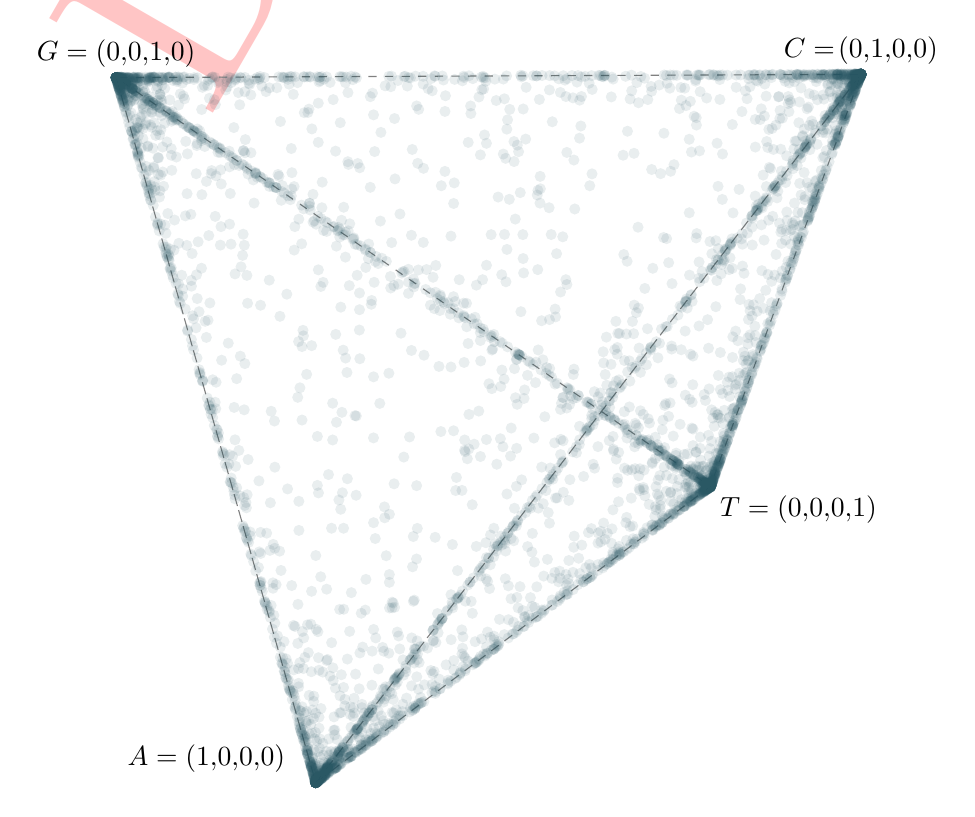
\begin{tikzpicture}[scale=10]


\begin{scope}[rotate around y=45,rotate around z=45]
 
% Draw the vertices of the tetrahedron

\coordinate (A) at (0, 0, 0);
\coordinate (C) at (1, 0, 0);
\coordinate (G) at (0.5, 0.866, 0);
\coordinate (T) at (0.5, 0.2887, 0.816);

%\foreach \p in {A,C,G,T}\fill[black] (\p) circle (0.02);

% Draw the edges of the cube
\draw[white!50!black, dashed]  (A) -- (C) -- (G) -- (A) -- (C) -- (T) -- (A) -- (T) -- (G) --  cycle;



    \pgfmathsetmacro{\alphaa}{0.1}       
       
\fill[color1,  opacity=\alphaa] (0.423,0.586,0.046) circle (.2pt);
         \fill[color1,  opacity=\alphaa] (0.984,0.027,0) circle (.2pt);
         \fill[color1,  opacity=\alphaa] (0.286,0.29,0.207) circle (.2pt);
         \fill[color1,  opacity=\alphaa] (0.842,0.106,0) circle (.2pt);
         \fill[color1,  opacity=\alphaa] (0.604,0.399,0.404) circle (.2pt);
         \fill[color1,  opacity=\alphaa] (0.093,0.02,0.057) circle (.2pt);
         \fill[color1,  opacity=\alphaa] (0,0,0) circle (.2pt);
         \fill[color1,  opacity=\alphaa] (0.231,0,0) circle (.2pt);
         \fill[color1,  opacity=\alphaa] (1,0,0) circle (.2pt);
         \fill[color1,  opacity=\alphaa] (0.36,0.556,0.003) circle (.2pt);
         \fill[color1,  opacity=\alphaa] (0.454,0.593,0.229) circle (.2pt);
         \fill[color1,  opacity=\alphaa] (0.506,0.85,0) circle (.2pt);
         \fill[color1,  opacity=\alphaa] (0.414,0.41,0.052) circle (.2pt);
         \fill[color1,  opacity=\alphaa] (0.533,0.269,0.762) circle (.2pt);
         \fill[color1,  opacity=\alphaa] (0.488,0.837,0) circle (.2pt);
         \fill[color1,  opacity=\alphaa] (0.001,0,0) circle (.2pt);
         \fill[color1,  opacity=\alphaa] (0.364,0.631,0) circle (.2pt);
         \fill[color1,  opacity=\alphaa] (0.495,0.836,0) circle (.2pt);
         \fill[color1,  opacity=\alphaa] (0.996,0.001,0) circle (.2pt);
         \fill[color1,  opacity=\alphaa] (0.999,0,0.001) circle (.2pt);
         \fill[color1,  opacity=\alphaa] (0.453,0.784,0) circle (.2pt);
         \fill[color1,  opacity=\alphaa] (0.405,0.235,0.66) circle (.2pt);
         \fill[color1,  opacity=\alphaa] (0.828,0.099,0.281) circle (.2pt);
         \fill[color1,  opacity=\alphaa] (0.648,0.186,0.526) circle (.2pt);
         \fill[color1,  opacity=\alphaa] (0.488,0.846,0) circle (.2pt);
         \fill[color1,  opacity=\alphaa] (0.47,0.438,0.499) circle (.2pt);
         \fill[color1,  opacity=\alphaa] (0.498,0.863,0) circle (.2pt);
         \fill[color1,  opacity=\alphaa] (0.006,0.01,0) circle (.2pt);
         \fill[color1,  opacity=\alphaa] (0.5,0.839,0.038) circle (.2pt);
         \fill[color1,  opacity=\alphaa] (0.605,0.051,0) circle (.2pt);
         \fill[color1,  opacity=\alphaa] (0.485,0.287,0.782) circle (.2pt);
         \fill[color1,  opacity=\alphaa] (0.516,0.502,0.418) circle (.2pt);
         \fill[color1,  opacity=\alphaa] (0.035,0.025,0.051) circle (.2pt);
         \fill[color1,  opacity=\alphaa] (0.5,0.289,0.816) circle (.2pt);
         \fill[color1,  opacity=\alphaa] (0.267,0.463,0) circle (.2pt);
         \fill[color1,  opacity=\alphaa] (0.5,0.289,0.816) circle (.2pt);
         \fill[color1,  opacity=\alphaa] (0.482,0.827,0) circle (.2pt);
         \fill[color1,  opacity=\alphaa] (0.5,0.298,0.804) circle (.2pt);
         \fill[color1,  opacity=\alphaa] (0.5,0.866,0) circle (.2pt);
         \fill[color1,  opacity=\alphaa] (0.5,0.289,0.816) circle (.2pt);
         \fill[color1,  opacity=\alphaa] (0.844,0.092,0.252) circle (.2pt);
         \fill[color1,  opacity=\alphaa] (0.476,0.583,0.341) circle (.2pt);
         \fill[color1,  opacity=\alphaa] (0.46,0.777,0.029) circle (.2pt);
         \fill[color1,  opacity=\alphaa] (0.996,0.007,0) circle (.2pt);
         \fill[color1,  opacity=\alphaa] (0.392,0.498,0.256) circle (.2pt);
         \fill[color1,  opacity=\alphaa] (0.977,0.013,0.038) circle (.2pt);
         \fill[color1,  opacity=\alphaa] (0.95,0.032,0.077) circle (.2pt);
         \fill[color1,  opacity=\alphaa] (0.436,0.611,0.002) circle (.2pt);
         \fill[color1,  opacity=\alphaa] (0.025,0.029,0.019) circle (.2pt);
         \fill[color1,  opacity=\alphaa] (0.952,0.028,0.079) circle (.2pt);
         \fill[color1,  opacity=\alphaa] (0.975,0.004,0.011) circle (.2pt);
         \fill[color1,  opacity=\alphaa] (0.006,0.002,0.006) circle (.2pt);
         \fill[color1,  opacity=\alphaa] (0.52,0.261,0.738) circle (.2pt);
         \fill[color1,  opacity=\alphaa] (0.319,0.184,0.521) circle (.2pt);
         \fill[color1,  opacity=\alphaa] (0.382,0.238,0.595) circle (.2pt);
         \fill[color1,  opacity=\alphaa] (0.207,0.357,0) circle (.2pt);
         \fill[color1,  opacity=\alphaa] (0.5,0.851,0.022) circle (.2pt);
         \fill[color1,  opacity=\alphaa] (0.575,0.22,0.616) circle (.2pt);
         \fill[color1,  opacity=\alphaa] (0.489,0.804,0.06) circle (.2pt);
         \fill[color1,  opacity=\alphaa] (0.968,0.006,0) circle (.2pt);
         \fill[color1,  opacity=\alphaa] (0.403,0,0) circle (.2pt);
         \fill[color1,  opacity=\alphaa] (0.008,0,0) circle (.2pt);
         \fill[color1,  opacity=\alphaa] (0.523,0.275,0.778) circle (.2pt);
         \fill[color1,  opacity=\alphaa] (0.5,0.474,0.554) circle (.2pt);
         \fill[color1,  opacity=\alphaa] (0.516,0.822,0.022) circle (.2pt);
         \fill[color1,  opacity=\alphaa] (0.021,0.001,0.003) circle (.2pt);
         \fill[color1,  opacity=\alphaa] (0.5,0.866,0) circle (.2pt);
         \fill[color1,  opacity=\alphaa] (0.339,0,0) circle (.2pt);
         \fill[color1,  opacity=\alphaa] (0.505,0.856,0.002) circle (.2pt);
         \fill[color1,  opacity=\alphaa] (0.002,0,0) circle (.2pt);
         \fill[color1,  opacity=\alphaa] (0.132,0.044,0.125) circle (.2pt);
         \fill[color1,  opacity=\alphaa] (0.508,0.851,0) circle (.2pt);
         \fill[color1,  opacity=\alphaa] (0,0,0) circle (.2pt);
         \fill[color1,  opacity=\alphaa] (0.831,0.29,0.003) circle (.2pt);
         \fill[color1,  opacity=\alphaa] (0,0,0) circle (.2pt);
         \fill[color1,  opacity=\alphaa] (0.502,0.301,0.793) circle (.2pt);
         \fill[color1,  opacity=\alphaa] (0.598,0.67,0.001) circle (.2pt);
         \fill[color1,  opacity=\alphaa] (0.5,0.846,0.028) circle (.2pt);
         \fill[color1,  opacity=\alphaa] (0.979,0.037,0) circle (.2pt);
         \fill[color1,  opacity=\alphaa] (0.548,0.78,0) circle (.2pt);
         \fill[color1,  opacity=\alphaa] (0.528,0.273,0.771) circle (.2pt);
         \fill[color1,  opacity=\alphaa] (0.445,0.769,0) circle (.2pt);
         \fill[color1,  opacity=\alphaa] (1,0,0) circle (.2pt);
         \fill[color1,  opacity=\alphaa] (0.461,0.264,0.748) circle (.2pt);
         \fill[color1,  opacity=\alphaa] (0.486,0.779,0.087) circle (.2pt);
         \fill[color1,  opacity=\alphaa] (0.074,0.018,0.034) circle (.2pt);
         \fill[color1,  opacity=\alphaa] (0.205,0.014,0.04) circle (.2pt);
         \fill[color1,  opacity=\alphaa] (0.501,0.288,0.815) circle (.2pt);
         \fill[color1,  opacity=\alphaa] (0.901,0.171,0) circle (.2pt);
         \fill[color1,  opacity=\alphaa] (0.5,0.305,0.793) circle (.2pt);
         \fill[color1,  opacity=\alphaa] (0.476,0.275,0.777) circle (.2pt);
         \fill[color1,  opacity=\alphaa] (0.563,0.749,0.011) circle (.2pt);
         \fill[color1,  opacity=\alphaa] (0.194,0.005,0.014) circle (.2pt);
         \fill[color1,  opacity=\alphaa] (0.5,0.289,0.816) circle (.2pt);
         \fill[color1,  opacity=\alphaa] (0.984,0,0) circle (.2pt);
         \fill[color1,  opacity=\alphaa] (0.97,0.016,0.013) circle (.2pt);
         \fill[color1,  opacity=\alphaa] (0.494,0.855,0) circle (.2pt);
         \fill[color1,  opacity=\alphaa] (0.497,0.287,0.811) circle (.2pt);
         \fill[color1,  opacity=\alphaa] (0.883,0.202,0) circle (.2pt);
         \fill[color1,  opacity=\alphaa] (0.305,0.055,0.001) circle (.2pt);
         \fill[color1,  opacity=\alphaa] (0.356,0.211,0.574) circle (.2pt);
         \fill[color1,  opacity=\alphaa] (0.02,0.035,0) circle (.2pt);
         \fill[color1,  opacity=\alphaa] (0.796,0.117,0.33) circle (.2pt);
         \fill[color1,  opacity=\alphaa] (0.391,0.161,0.43) circle (.2pt);
         \fill[color1,  opacity=\alphaa] (0.099,0.001,0) circle (.2pt);
         \fill[color1,  opacity=\alphaa] (0,0,0) circle (.2pt);
         \fill[color1,  opacity=\alphaa] (0.483,0.411,0.603) circle (.2pt);
         \fill[color1,  opacity=\alphaa] (0.5,0.289,0.816) circle (.2pt);
         \fill[color1,  opacity=\alphaa] (0.499,0.288,0.815) circle (.2pt);
         \fill[color1,  opacity=\alphaa] (0.499,0.864,0) circle (.2pt);
         \fill[color1,  opacity=\alphaa] (0.496,0.285,0.807) circle (.2pt);
         \fill[color1,  opacity=\alphaa] (0.493,0.852,0.002) circle (.2pt);
         \fill[color1,  opacity=\alphaa] (0.501,0.296,0.803) circle (.2pt);
         \fill[color1,  opacity=\alphaa] (0.155,0.26,0) circle (.2pt);
         \fill[color1,  opacity=\alphaa] (0.493,0.285,0.806) circle (.2pt);
         \fill[color1,  opacity=\alphaa] (0.581,0.14,0.377) circle (.2pt);
         \fill[color1,  opacity=\alphaa] (0.738,0,0) circle (.2pt);
         \fill[color1,  opacity=\alphaa] (0.655,0.199,0.563) circle (.2pt);
         \fill[color1,  opacity=\alphaa] (0.492,0.694,0.221) circle (.2pt);
         \fill[color1,  opacity=\alphaa] (0.502,0.86,0.004) circle (.2pt);
         \fill[color1,  opacity=\alphaa] (0.725,0.023,0.066) circle (.2pt);
         \fill[color1,  opacity=\alphaa] (0.029,0.049,0) circle (.2pt);
         \fill[color1,  opacity=\alphaa] (0.262,0,0) circle (.2pt);
         \fill[color1,  opacity=\alphaa] (0.382,0.368,0.414) circle (.2pt);
         \fill[color1,  opacity=\alphaa] (0.999,0.001,0.002) circle (.2pt);
         \fill[color1,  opacity=\alphaa] (0.5,0.313,0.783) circle (.2pt);
         \fill[color1,  opacity=\alphaa] (0.999,0,0) circle (.2pt);
         \fill[color1,  opacity=\alphaa] (0.496,0.858,0.001) circle (.2pt);
         \fill[color1,  opacity=\alphaa] (0.71,0.171,0.469) circle (.2pt);
         \fill[color1,  opacity=\alphaa] (0.025,0.014,0.041) circle (.2pt);
         \fill[color1,  opacity=\alphaa] (0.049,0,0) circle (.2pt);
         \fill[color1,  opacity=\alphaa] (0.439,0.15,0.424) circle (.2pt);
         \fill[color1,  opacity=\alphaa] (0.261,0.151,0.418) circle (.2pt);
         \fill[color1,  opacity=\alphaa] (0,0,0) circle (.2pt);
         \fill[color1,  opacity=\alphaa] (0.5,0.864,0.002) circle (.2pt);
         \fill[color1,  opacity=\alphaa] (0.347,0.427,0.242) circle (.2pt);
         \fill[color1,  opacity=\alphaa] (0.95,0.029,0.081) circle (.2pt);
         \fill[color1,  opacity=\alphaa] (1,0,0) circle (.2pt);
         \fill[color1,  opacity=\alphaa] (0.988,0.02,0) circle (.2pt);
         \fill[color1,  opacity=\alphaa] (0.784,0.124,0.35) circle (.2pt);
         \fill[color1,  opacity=\alphaa] (0.468,0.274,0.759) circle (.2pt);
         \fill[color1,  opacity=\alphaa] (0.286,0.093,0.263) circle (.2pt);
         \fill[color1,  opacity=\alphaa] (0.493,0.847,0.009) circle (.2pt);
         \fill[color1,  opacity=\alphaa] (0.927,0,0) circle (.2pt);
         \fill[color1,  opacity=\alphaa] (0.429,0,0) circle (.2pt);
         \fill[color1,  opacity=\alphaa] (0.916,0.047,0.133) circle (.2pt);
         \fill[color1,  opacity=\alphaa] (0.613,0,0.001) circle (.2pt);
         \fill[color1,  opacity=\alphaa] (0.5,0.327,0.763) circle (.2pt);
         \fill[color1,  opacity=\alphaa] (0.963,0.007,0) circle (.2pt);
         \fill[color1,  opacity=\alphaa] (0.534,0.268,0.759) circle (.2pt);
         \fill[color1,  opacity=\alphaa] (0.483,0.309,0.747) circle (.2pt);
         \fill[color1,  opacity=\alphaa] (0.499,0.865,0) circle (.2pt);
         \fill[color1,  opacity=\alphaa] (0.285,0.452,0.057) circle (.2pt);
         \fill[color1,  opacity=\alphaa] (0.848,0.088,0.247) circle (.2pt);
         \fill[color1,  opacity=\alphaa] (0.118,0.203,0.003) circle (.2pt);
         \fill[color1,  opacity=\alphaa] (1,0,0) circle (.2pt);
         \fill[color1,  opacity=\alphaa] (0.261,0.018,0.05) circle (.2pt);
         \fill[color1,  opacity=\alphaa] (0.5,0.866,0) circle (.2pt);
         \fill[color1,  opacity=\alphaa] (0.5,0.339,0.744) circle (.2pt);
         \fill[color1,  opacity=\alphaa] (0.066,0.113,0) circle (.2pt);
         \fill[color1,  opacity=\alphaa] (0.507,0.285,0.806) circle (.2pt);
         \fill[color1,  opacity=\alphaa] (0.023,0.004,0.01) circle (.2pt);
         \fill[color1,  opacity=\alphaa] (0.139,0.148,0) circle (.2pt);
         \fill[color1,  opacity=\alphaa] (0.507,0.332,0.74) circle (.2pt);
         \fill[color1,  opacity=\alphaa] (0.5,0.865,0.001) circle (.2pt);
         \fill[color1,  opacity=\alphaa] (0.5,0.301,0.799) circle (.2pt);
         \fill[color1,  opacity=\alphaa] (0.012,0.021,0) circle (.2pt);
         \fill[color1,  opacity=\alphaa] (0.459,0.767,0) circle (.2pt);
         \fill[color1,  opacity=\alphaa] (0.779,0.128,0.36) circle (.2pt);
         \fill[color1,  opacity=\alphaa] (0.5,0.699,0.236) circle (.2pt);
         \fill[color1,  opacity=\alphaa] (0.868,0.229,0) circle (.2pt);
         \fill[color1,  opacity=\alphaa] (0.004,0,0) circle (.2pt);
         \fill[color1,  opacity=\alphaa] (0.5,0.663,0.288) circle (.2pt);
         \fill[color1,  opacity=\alphaa] (0.496,0.507,0.498) circle (.2pt);
         \fill[color1,  opacity=\alphaa] (0.184,0.289,0.043) circle (.2pt);
         \fill[color1,  opacity=\alphaa] (0.5,0.863,0.004) circle (.2pt);
         \fill[color1,  opacity=\alphaa] (0.955,0.032,0.066) circle (.2pt);
         \fill[color1,  opacity=\alphaa] (0.484,0.838,0.002) circle (.2pt);
         \fill[color1,  opacity=\alphaa] (0.043,0.074,0) circle (.2pt);
         \fill[color1,  opacity=\alphaa] (0.501,0.31,0.784) circle (.2pt);
         \fill[color1,  opacity=\alphaa] (0.992,0.009,0) circle (.2pt);
         \fill[color1,  opacity=\alphaa] (0.491,0.851,0) circle (.2pt);
         \fill[color1,  opacity=\alphaa] (0.499,0.291,0.809) circle (.2pt);
         \fill[color1,  opacity=\alphaa] (0,0,0) circle (.2pt);
         \fill[color1,  opacity=\alphaa] (0.047,0.012,0.033) circle (.2pt);
         \fill[color1,  opacity=\alphaa] (0.961,0.067,0) circle (.2pt);
         \fill[color1,  opacity=\alphaa] (0.502,0.287,0.813) circle (.2pt);
         \fill[color1,  opacity=\alphaa] (0.499,0.288,0.814) circle (.2pt);
         \fill[color1,  opacity=\alphaa] (0.181,0.161,0) circle (.2pt);
         \fill[color1,  opacity=\alphaa] (0.455,0.783,0.001) circle (.2pt);
         \fill[color1,  opacity=\alphaa] (0.875,0,0) circle (.2pt);
         \fill[color1,  opacity=\alphaa] (0.505,0.304,0.782) circle (.2pt);
         \fill[color1,  opacity=\alphaa] (0.66,0.221,0.519) circle (.2pt);
         \fill[color1,  opacity=\alphaa] (0.564,0.252,0.712) circle (.2pt);
         \fill[color1,  opacity=\alphaa] (0.5,0.289,0.816) circle (.2pt);
         \fill[color1,  opacity=\alphaa] (0.5,0.289,0.816) circle (.2pt);
         \fill[color1,  opacity=\alphaa] (0.667,0.325,0.355) circle (.2pt);
         \fill[color1,  opacity=\alphaa] (1,0,0) circle (.2pt);
         \fill[color1,  opacity=\alphaa] (0.406,0.454,0.29) circle (.2pt);
         \fill[color1,  opacity=\alphaa] (0.55,0.776,0.004) circle (.2pt);
         \fill[color1,  opacity=\alphaa] (0.309,0.179,0.505) circle (.2pt);
         \fill[color1,  opacity=\alphaa] (0.5,0.861,0.007) circle (.2pt);
         \fill[color1,  opacity=\alphaa] (0.47,0.723,0.127) circle (.2pt);
         \fill[color1,  opacity=\alphaa] (0.061,0.03,0.083) circle (.2pt);
         \fill[color1,  opacity=\alphaa] (1,0,0) circle (.2pt);
         \fill[color1,  opacity=\alphaa] (0.5,0.288,0.816) circle (.2pt);
         \fill[color1,  opacity=\alphaa] (0.001,0,0) circle (.2pt);
         \fill[color1,  opacity=\alphaa] (0.5,0.865,0) circle (.2pt);
         \fill[color1,  opacity=\alphaa] (0.883,0.203,0) circle (.2pt);
         \fill[color1,  opacity=\alphaa] (0.224,0,0) circle (.2pt);
         \fill[color1,  opacity=\alphaa] (0.849,0.234,0) circle (.2pt);
         \fill[color1,  opacity=\alphaa] (0.484,0,0) circle (.2pt);
         \fill[color1,  opacity=\alphaa] (0.732,0.154,0.437) circle (.2pt);
         \fill[color1,  opacity=\alphaa] (0.998,0.001,0.004) circle (.2pt);
         \fill[color1,  opacity=\alphaa] (0.46,0.424,0.526) circle (.2pt);
         \fill[color1,  opacity=\alphaa] (0.524,0.825,0) circle (.2pt);
         \fill[color1,  opacity=\alphaa] (0.531,0.026,0.054) circle (.2pt);
         \fill[color1,  opacity=\alphaa] (0.022,0.001,0) circle (.2pt);
         \fill[color1,  opacity=\alphaa] (0.733,0.037,0.099) circle (.2pt);
         \fill[color1,  opacity=\alphaa] (0.5,0.339,0.745) circle (.2pt);
         \fill[color1,  opacity=\alphaa] (0.993,0.013,0) circle (.2pt);
         \fill[color1,  opacity=\alphaa] (0.5,0.857,0.013) circle (.2pt);
         \fill[color1,  opacity=\alphaa] (0.995,0.001,0.001) circle (.2pt);
         \fill[color1,  opacity=\alphaa] (0.075,0.103,0.039) circle (.2pt);
         \fill[color1,  opacity=\alphaa] (0.994,0.003,0.009) circle (.2pt);
         \fill[color1,  opacity=\alphaa] (0.855,0.021,0) circle (.2pt);
         \fill[color1,  opacity=\alphaa] (0.5,0.856,0.014) circle (.2pt);
         \fill[color1,  opacity=\alphaa] (0.995,0.003,0.008) circle (.2pt);
         \fill[color1,  opacity=\alphaa] (1,0,0) circle (.2pt);
         \fill[color1,  opacity=\alphaa] (0.002,0.001,0) circle (.2pt);
         \fill[color1,  opacity=\alphaa] (0.994,0,0.001) circle (.2pt);
         \fill[color1,  opacity=\alphaa] (0.493,0.281,0.794) circle (.2pt);
         \fill[color1,  opacity=\alphaa] (0.825,0.303,0) circle (.2pt);
         \fill[color1,  opacity=\alphaa] (0.501,0.859,0.008) circle (.2pt);
         \fill[color1,  opacity=\alphaa] (0.496,0.286,0.808) circle (.2pt);
         \fill[color1,  opacity=\alphaa] (0.497,0.283,0.799) circle (.2pt);
         \fill[color1,  opacity=\alphaa] (0.501,0.288,0.814) circle (.2pt);
         \fill[color1,  opacity=\alphaa] (0.502,0.298,0.798) circle (.2pt);
         \fill[color1,  opacity=\alphaa] (0.229,0.059,0.017) circle (.2pt);
         \fill[color1,  opacity=\alphaa] (0.5,0.858,0.011) circle (.2pt);
         \fill[color1,  opacity=\alphaa] (0.5,0.866,0) circle (.2pt);
         \fill[color1,  opacity=\alphaa] (0.17,0.06,0) circle (.2pt);
         \fill[color1,  opacity=\alphaa] (0.398,0.686,0.006) circle (.2pt);
         \fill[color1,  opacity=\alphaa] (0.949,0.071,0) circle (.2pt);
         \fill[color1,  opacity=\alphaa] (0.5,0.289,0.816) circle (.2pt);
         \fill[color1,  opacity=\alphaa] (0.976,0.03,0) circle (.2pt);
         \fill[color1,  opacity=\alphaa] (0.286,0.109,0.003) circle (.2pt);
         \fill[color1,  opacity=\alphaa] (0.002,0.001,0.002) circle (.2pt);
         \fill[color1,  opacity=\alphaa] (0.345,0.559,0) circle (.2pt);
         \fill[color1,  opacity=\alphaa] (0.456,0.633,0.219) circle (.2pt);
         \fill[color1,  opacity=\alphaa] (0.499,0.833,0.045) circle (.2pt);
         \fill[color1,  opacity=\alphaa] (0.01,0.005,0.002) circle (.2pt);
         \fill[color1,  opacity=\alphaa] (0.491,0.33,0.735) circle (.2pt);
         \fill[color1,  opacity=\alphaa] (0.554,0.752,0) circle (.2pt);
         \fill[color1,  opacity=\alphaa] (0.493,0.854,0) circle (.2pt);
         \fill[color1,  opacity=\alphaa] (0.999,0.001,0) circle (.2pt);
         \fill[color1,  opacity=\alphaa] (0.984,0.028,0) circle (.2pt);
         \fill[color1,  opacity=\alphaa] (0.999,0,0) circle (.2pt);
         \fill[color1,  opacity=\alphaa] (0.071,0.041,0.117) circle (.2pt);
         \fill[color1,  opacity=\alphaa] (0,0,0) circle (.2pt);
         \fill[color1,  opacity=\alphaa] (0.572,0.649,0.13) circle (.2pt);
         \fill[color1,  opacity=\alphaa] (0.406,0.235,0.662) circle (.2pt);
         \fill[color1,  opacity=\alphaa] (0.001,0.001,0.001) circle (.2pt);
         \fill[color1,  opacity=\alphaa] (0.998,0.001,0.003) circle (.2pt);
         \fill[color1,  opacity=\alphaa] (0.334,0,0) circle (.2pt);
         \fill[color1,  opacity=\alphaa] (0.989,0,0) circle (.2pt);
         \fill[color1,  opacity=\alphaa] (0.716,0.485,0.005) circle (.2pt);
         \fill[color1,  opacity=\alphaa] (0.002,0.004,0) circle (.2pt);
         \fill[color1,  opacity=\alphaa] (0.948,0.033,0.08) circle (.2pt);
         \fill[color1,  opacity=\alphaa] (0.996,0.002,0.007) circle (.2pt);
         \fill[color1,  opacity=\alphaa] (0.03,0.048,0) circle (.2pt);
         \fill[color1,  opacity=\alphaa] (0.503,0.335,0.744) circle (.2pt);
         \fill[color1,  opacity=\alphaa] (0.241,0.001,0) circle (.2pt);
         \fill[color1,  opacity=\alphaa] (0.063,0,0) circle (.2pt);
         \fill[color1,  opacity=\alphaa] (0.5,0.289,0.816) circle (.2pt);
         \fill[color1,  opacity=\alphaa] (0,0,0) circle (.2pt);
         \fill[color1,  opacity=\alphaa] (0.026,0,0) circle (.2pt);
         \fill[color1,  opacity=\alphaa] (0.021,0.037,0) circle (.2pt);
         \fill[color1,  opacity=\alphaa] (0.511,0.836,0.013) circle (.2pt);
         \fill[color1,  opacity=\alphaa] (0.953,0.027,0.076) circle (.2pt);
         \fill[color1,  opacity=\alphaa] (0.013,0,0) circle (.2pt);
         \fill[color1,  opacity=\alphaa] (0.452,0.288,0.7) circle (.2pt);
         \fill[color1,  opacity=\alphaa] (0.004,0.002,0.006) circle (.2pt);
         \fill[color1,  opacity=\alphaa] (0.455,0.055,0) circle (.2pt);
         \fill[color1,  opacity=\alphaa] (0.775,0.13,0.367) circle (.2pt);
         \fill[color1,  opacity=\alphaa] (0.5,0.289,0.816) circle (.2pt);
         \fill[color1,  opacity=\alphaa] (0.841,0,0) circle (.2pt);
         \fill[color1,  opacity=\alphaa] (0.732,0.004,0.009) circle (.2pt);
         \fill[color1,  opacity=\alphaa] (0.488,0.282,0.797) circle (.2pt);
         \fill[color1,  opacity=\alphaa] (0.003,0.005,0) circle (.2pt);
         \fill[color1,  opacity=\alphaa] (0.5,0.866,0.001) circle (.2pt);
         \fill[color1,  opacity=\alphaa] (0.513,0.281,0.796) circle (.2pt);
         \fill[color1,  opacity=\alphaa] (0.497,0.31,0.778) circle (.2pt);
         \fill[color1,  opacity=\alphaa] (0.83,0.289,0.007) circle (.2pt);
         \fill[color1,  opacity=\alphaa] (0.501,0.288,0.814) circle (.2pt);
         \fill[color1,  opacity=\alphaa] (0.5,0.29,0.815) circle (.2pt);
         \fill[color1,  opacity=\alphaa] (0.971,0.02,0.041) circle (.2pt);
         \fill[color1,  opacity=\alphaa] (0,0,0) circle (.2pt);
         \fill[color1,  opacity=\alphaa] (0.513,0.82,0.034) circle (.2pt);
         \fill[color1,  opacity=\alphaa] (0.518,0.67,0.234) circle (.2pt);
         \fill[color1,  opacity=\alphaa] (0.989,0.006,0.018) circle (.2pt);
         \fill[color1,  opacity=\alphaa] (1,0,0) circle (.2pt);
         \fill[color1,  opacity=\alphaa] (0.5,0.854,0.017) circle (.2pt);
         \fill[color1,  opacity=\alphaa] (0.501,0.797,0.059) circle (.2pt);
         \fill[color1,  opacity=\alphaa] (0.783,0.139,0.335) circle (.2pt);
         \fill[color1,  opacity=\alphaa] (0.194,0.135,0.01) circle (.2pt);
         \fill[color1,  opacity=\alphaa] (0.504,0.86,0) circle (.2pt);
         \fill[color1,  opacity=\alphaa] (0.915,0.049,0.139) circle (.2pt);
         \fill[color1,  opacity=\alphaa] (0.006,0.003,0.01) circle (.2pt);
         \fill[color1,  opacity=\alphaa] (0.5,0.393,0.669) circle (.2pt);
         \fill[color1,  opacity=\alphaa] (0.001,0,0.001) circle (.2pt);
         \fill[color1,  opacity=\alphaa] (0.916,0.089,0.065) circle (.2pt);
         \fill[color1,  opacity=\alphaa] (0.003,0,0) circle (.2pt);
         \fill[color1,  opacity=\alphaa] (0.552,0.216,0.612) circle (.2pt);
         \fill[color1,  opacity=\alphaa] (0.987,0.023,0) circle (.2pt);
         \fill[color1,  opacity=\alphaa] (0.883,0,0) circle (.2pt);
         \fill[color1,  opacity=\alphaa] (0.362,0,0) circle (.2pt);
         \fill[color1,  opacity=\alphaa] (0.952,0.003,0.003) circle (.2pt);
         \fill[color1,  opacity=\alphaa] (0.091,0.151,0.009) circle (.2pt);
         \fill[color1,  opacity=\alphaa] (0.426,0.733,0.007) circle (.2pt);
         \fill[color1,  opacity=\alphaa] (0.5,0.861,0.007) circle (.2pt);
         \fill[color1,  opacity=\alphaa] (0.5,0.289,0.816) circle (.2pt);
         \fill[color1,  opacity=\alphaa] (0.62,0.658,0) circle (.2pt);
         \fill[color1,  opacity=\alphaa] (0.785,0.341,0.044) circle (.2pt);
         \fill[color1,  opacity=\alphaa] (0.004,0.007,0) circle (.2pt);
         \fill[color1,  opacity=\alphaa] (0.702,0.185,0.416) circle (.2pt);
         \fill[color1,  opacity=\alphaa] (0.071,0.041,0.116) circle (.2pt);
         \fill[color1,  opacity=\alphaa] (0.498,0.311,0.781) circle (.2pt);
         \fill[color1,  opacity=\alphaa] (0.499,0.86,0.006) circle (.2pt);
         \fill[color1,  opacity=\alphaa] (0.508,0.85,0) circle (.2pt);
         \fill[color1,  opacity=\alphaa] (0.006,0,0) circle (.2pt);
         \fill[color1,  opacity=\alphaa] (0.523,0.826,0) circle (.2pt);
         \fill[color1,  opacity=\alphaa] (0.001,0,0) circle (.2pt);
         \fill[color1,  opacity=\alphaa] (0.49,0.087,0.243) circle (.2pt);
         \fill[color1,  opacity=\alphaa] (0.5,0.857,0.013) circle (.2pt);
         \fill[color1,  opacity=\alphaa] (0.5,0.771,0.134) circle (.2pt);
         \fill[color1,  opacity=\alphaa] (0.444,0.365,0.572) circle (.2pt);
         \fill[color1,  opacity=\alphaa] (0.313,0.175,0.494) circle (.2pt);
         \fill[color1,  opacity=\alphaa] (0.497,0.287,0.812) circle (.2pt);
         \fill[color1,  opacity=\alphaa] (0.167,0.096,0.273) circle (.2pt);
         \fill[color1,  opacity=\alphaa] (0.5,0.528,0.477) circle (.2pt);
         \fill[color1,  opacity=\alphaa] (0.473,0.791,0.039) circle (.2pt);
         \fill[color1,  opacity=\alphaa] (0.892,0.187,0) circle (.2pt);
         \fill[color1,  opacity=\alphaa] (0.187,0.003,0) circle (.2pt);
         \fill[color1,  opacity=\alphaa] (0.497,0.857,0) circle (.2pt);
         \fill[color1,  opacity=\alphaa] (1,0,0) circle (.2pt);
         \fill[color1,  opacity=\alphaa] (0.031,0.018,0.051) circle (.2pt);
         \fill[color1,  opacity=\alphaa] (0.495,0.857,0) circle (.2pt);
         \fill[color1,  opacity=\alphaa] (0.807,0.3,0) circle (.2pt);
         \fill[color1,  opacity=\alphaa] (0.226,0.131,0.37) circle (.2pt);
         \fill[color1,  opacity=\alphaa] (0.984,0,0) circle (.2pt);
         \fill[color1,  opacity=\alphaa] (0.498,0.288,0.813) circle (.2pt);
         \fill[color1,  opacity=\alphaa] (0.011,0.019,0) circle (.2pt);
         \fill[color1,  opacity=\alphaa] (0.5,0.289,0.816) circle (.2pt);
         \fill[color1,  opacity=\alphaa] (0.936,0.11,0) circle (.2pt);
         \fill[color1,  opacity=\alphaa] (0.491,0.283,0.801) circle (.2pt);
         \fill[color1,  opacity=\alphaa] (0.419,0.242,0.675) circle (.2pt);
         \fill[color1,  opacity=\alphaa] (0.538,0.267,0.754) circle (.2pt);
         \fill[color1,  opacity=\alphaa] (0.501,0.288,0.814) circle (.2pt);
         \fill[color1,  opacity=\alphaa] (0.5,0.355,0.722) circle (.2pt);
         \fill[color1,  opacity=\alphaa] (0,0.001,0) circle (.2pt);
         \fill[color1,  opacity=\alphaa] (0.286,0.165,0.467) circle (.2pt);
         \fill[color1,  opacity=\alphaa] (0.5,0.67,0.277) circle (.2pt);
         \fill[color1,  opacity=\alphaa] (0.03,0,0) circle (.2pt);
         \fill[color1,  opacity=\alphaa] (0.072,0.035,0.099) circle (.2pt);
         \fill[color1,  opacity=\alphaa] (0.491,0.283,0.8) circle (.2pt);
         \fill[color1,  opacity=\alphaa] (0.113,0.146,0) circle (.2pt);
         \fill[color1,  opacity=\alphaa] (0.5,0.445,0.594) circle (.2pt);
         \fill[color1,  opacity=\alphaa] (0.246,0.426,0) circle (.2pt);
         \fill[color1,  opacity=\alphaa] (0.528,0.219,0.618) circle (.2pt);
         \fill[color1,  opacity=\alphaa] (0.985,0.012,0.021) circle (.2pt);
         \fill[color1,  opacity=\alphaa] (0.503,0.291,0.803) circle (.2pt);
         \fill[color1,  opacity=\alphaa] (0.5,0.85,0.023) circle (.2pt);
         \fill[color1,  opacity=\alphaa] (0.201,0.339,0.012) circle (.2pt);
         \fill[color1,  opacity=\alphaa] (0.5,0.766,0.141) circle (.2pt);
         \fill[color1,  opacity=\alphaa] (0.069,0.075,0.063) circle (.2pt);
         \fill[color1,  opacity=\alphaa] (0.999,0,0.001) circle (.2pt);
         \fill[color1,  opacity=\alphaa] (0.722,0.161,0.454) circle (.2pt);
         \fill[color1,  opacity=\alphaa] (0.501,0.3,0.798) circle (.2pt);
         \fill[color1,  opacity=\alphaa] (0.264,0.153,0.432) circle (.2pt);
         \fill[color1,  opacity=\alphaa] (0.077,0,0) circle (.2pt);
         \fill[color1,  opacity=\alphaa] (0.812,0.088,0.239) circle (.2pt);
         \fill[color1,  opacity=\alphaa] (0.565,0.488,0.376) circle (.2pt);
         \fill[color1,  opacity=\alphaa] (0.968,0.055,0) circle (.2pt);
         \fill[color1,  opacity=\alphaa] (0,0,0.001) circle (.2pt);
         \fill[color1,  opacity=\alphaa] (0.526,0.822,0) circle (.2pt);
         \fill[color1,  opacity=\alphaa] (0.467,0.27,0.762) circle (.2pt);
         \fill[color1,  opacity=\alphaa] (0.025,0,0) circle (.2pt);
         \fill[color1,  opacity=\alphaa] (0.5,0.325,0.765) circle (.2pt);
         \fill[color1,  opacity=\alphaa] (0.257,0.301,0.143) circle (.2pt);
         \fill[color1,  opacity=\alphaa] (0.009,0,0.001) circle (.2pt);
         \fill[color1,  opacity=\alphaa] (0.686,0.53,0.019) circle (.2pt);
         \fill[color1,  opacity=\alphaa] (0.5,0.866,0) circle (.2pt);
         \fill[color1,  opacity=\alphaa] (0.735,0.191,0.38) circle (.2pt);
         \fill[color1,  opacity=\alphaa] (0.499,0.864,0) circle (.2pt);
         \fill[color1,  opacity=\alphaa] (0,0,0) circle (.2pt);
         \fill[color1,  opacity=\alphaa] (0.971,0.051,0) circle (.2pt);
         \fill[color1,  opacity=\alphaa] (0.934,0.047,0) circle (.2pt);
         \fill[color1,  opacity=\alphaa] (0.5,0.501,0.517) circle (.2pt);
         \fill[color1,  opacity=\alphaa] (0.125,0.189,0.037) circle (.2pt);
         \fill[color1,  opacity=\alphaa] (0.5,0.861,0.006) circle (.2pt);
         \fill[color1,  opacity=\alphaa] (0.5,0.788,0.109) circle (.2pt);
         \fill[color1,  opacity=\alphaa] (0.003,0.003,0.002) circle (.2pt);
         \fill[color1,  opacity=\alphaa] (0.501,0.865,0) circle (.2pt);
         \fill[color1,  opacity=\alphaa] (0.931,0.072,0.012) circle (.2pt);
         \fill[color1,  opacity=\alphaa] (0.5,0.865,0) circle (.2pt);
         \fill[color1,  opacity=\alphaa] (1,0.001,0) circle (.2pt);
         \fill[color1,  opacity=\alphaa] (0.004,0.007,0) circle (.2pt);
         \fill[color1,  opacity=\alphaa] (0.237,0.395,0) circle (.2pt);
         \fill[color1,  opacity=\alphaa] (0.499,0.294,0.807) circle (.2pt);
         \fill[color1,  opacity=\alphaa] (0.516,0.28,0.791) circle (.2pt);
         \fill[color1,  opacity=\alphaa] (0.461,0.172,0.486) circle (.2pt);
         \fill[color1,  opacity=\alphaa] (0.454,0.262,0.741) circle (.2pt);
         \fill[color1,  opacity=\alphaa] (0.013,0,0) circle (.2pt);
         \fill[color1,  opacity=\alphaa] (0.409,0.238,0.665) circle (.2pt);
         \fill[color1,  opacity=\alphaa] (0.5,0.866,0) circle (.2pt);
         \fill[color1,  opacity=\alphaa] (0.485,0.363,0.674) circle (.2pt);
         \fill[color1,  opacity=\alphaa] (0.489,0.417,0.608) circle (.2pt);
         \fill[color1,  opacity=\alphaa] (1,0,0) circle (.2pt);
         \fill[color1,  opacity=\alphaa] (0.001,0.001,0) circle (.2pt);
         \fill[color1,  opacity=\alphaa] (0.497,0.287,0.812) circle (.2pt);
         \fill[color1,  opacity=\alphaa] (0.037,0.005,0.014) circle (.2pt);
         \fill[color1,  opacity=\alphaa] (0.85,0.084,0.237) circle (.2pt);
         \fill[color1,  opacity=\alphaa] (0.46,0.537,0.286) circle (.2pt);
         \fill[color1,  opacity=\alphaa] (0.5,0.289,0.816) circle (.2pt);
         \fill[color1,  opacity=\alphaa] (0.5,0.289,0.816) circle (.2pt);
         \fill[color1,  opacity=\alphaa] (0.488,0.843,0.003) circle (.2pt);
         \fill[color1,  opacity=\alphaa] (0.482,0.278,0.783) circle (.2pt);
         \fill[color1,  opacity=\alphaa] (0.54,0.318,0.677) circle (.2pt);
         \fill[color1,  opacity=\alphaa] (0.5,0.289,0.816) circle (.2pt);
         \fill[color1,  opacity=\alphaa] (0.491,0.808,0) circle (.2pt);
         \fill[color1,  opacity=\alphaa] (0.727,0,0) circle (.2pt);
         \fill[color1,  opacity=\alphaa] (0,0,0) circle (.2pt);
         \fill[color1,  opacity=\alphaa] (0.699,0.174,0.491) circle (.2pt);
         \fill[color1,  opacity=\alphaa] (0,0,0) circle (.2pt);
         \fill[color1,  opacity=\alphaa] (0.5,0.865,0.001) circle (.2pt);
         \fill[color1,  opacity=\alphaa] (0.996,0.006,0.001) circle (.2pt);
         \fill[color1,  opacity=\alphaa] (0.901,0.172,0) circle (.2pt);
         \fill[color1,  opacity=\alphaa] (0.466,0.64,0.236) circle (.2pt);
         \fill[color1,  opacity=\alphaa] (0.062,0.034,0.094) circle (.2pt);
         \fill[color1,  opacity=\alphaa] (0.986,0.023,0) circle (.2pt);
         \fill[color1,  opacity=\alphaa] (0.997,0.002,0.005) circle (.2pt);
         \fill[color1,  opacity=\alphaa] (0.499,0.288,0.814) circle (.2pt);
         \fill[color1,  opacity=\alphaa] (0.963,0,0) circle (.2pt);
         \fill[color1,  opacity=\alphaa] (0,0,0) circle (.2pt);
         \fill[color1,  opacity=\alphaa] (0.354,0.339,0.387) circle (.2pt);
         \fill[color1,  opacity=\alphaa] (0.471,0.372,0.628) circle (.2pt);
         \fill[color1,  opacity=\alphaa] (0.971,0.017,0.046) circle (.2pt);
         \fill[color1,  opacity=\alphaa] (0.49,0.281,0.795) circle (.2pt);
         \fill[color1,  opacity=\alphaa] (0.583,0.722,0.001) circle (.2pt);
         \fill[color1,  opacity=\alphaa] (0.487,0.844,0) circle (.2pt);
         \fill[color1,  opacity=\alphaa] (0.129,0.217,0.01) circle (.2pt);
         \fill[color1,  opacity=\alphaa] (0.998,0,0) circle (.2pt);
         \fill[color1,  opacity=\alphaa] (0.504,0.86,0) circle (.2pt);
         \fill[color1,  opacity=\alphaa] (0,0,0) circle (.2pt);
         \fill[color1,  opacity=\alphaa] (0.5,0.289,0.816) circle (.2pt);
         \fill[color1,  opacity=\alphaa] (0.896,0.002,0.005) circle (.2pt);
         \fill[color1,  opacity=\alphaa] (0.961,0.066,0.002) circle (.2pt);
         \fill[color1,  opacity=\alphaa] (0.554,0.313,0.651) circle (.2pt);
         \fill[color1,  opacity=\alphaa] (0.502,0.861,0) circle (.2pt);
         \fill[color1,  opacity=\alphaa] (0.587,0.278,0.609) circle (.2pt);
         \fill[color1,  opacity=\alphaa] (0.487,0.819,0.033) circle (.2pt);
         \fill[color1,  opacity=\alphaa] (0.457,0.791,0) circle (.2pt);
         \fill[color1,  opacity=\alphaa] (0.5,0.425,0.623) circle (.2pt);
         \fill[color1,  opacity=\alphaa] (0.426,0.235,0.663) circle (.2pt);
         \fill[color1,  opacity=\alphaa] (0.511,0,0) circle (.2pt);
         \fill[color1,  opacity=\alphaa] (0.023,0,0) circle (.2pt);
         \fill[color1,  opacity=\alphaa] (0.518,0.829,0.009) circle (.2pt);
         \fill[color1,  opacity=\alphaa] (0.877,0.002,0) circle (.2pt);
         \fill[color1,  opacity=\alphaa] (0.604,0.228,0.646) circle (.2pt);
         \fill[color1,  opacity=\alphaa] (0.027,0.042,0) circle (.2pt);
         \fill[color1,  opacity=\alphaa] (0.976,0.039,0) circle (.2pt);
         \fill[color1,  opacity=\alphaa] (0.497,0.291,0.806) circle (.2pt);
         \fill[color1,  opacity=\alphaa] (0.496,0.571,0.406) circle (.2pt);
         \fill[color1,  opacity=\alphaa] (0.558,0.371,0.385) circle (.2pt);
         \fill[color1,  opacity=\alphaa] (0.5,0.35,0.729) circle (.2pt);
         \fill[color1,  opacity=\alphaa] (0.268,0.265,0) circle (.2pt);
         \fill[color1,  opacity=\alphaa] (0.015,0.025,0) circle (.2pt);
         \fill[color1,  opacity=\alphaa] (0.487,0.449,0.558) circle (.2pt);
         \fill[color1,  opacity=\alphaa] (1,0,0) circle (.2pt);
         \fill[color1,  opacity=\alphaa] (0.989,0.006,0.017) circle (.2pt);
         \fill[color1,  opacity=\alphaa] (0.442,0.489,0.391) circle (.2pt);
         \fill[color1,  opacity=\alphaa] (0.508,0.85,0.003) circle (.2pt);
         \fill[color1,  opacity=\alphaa] (0.124,0.024,0.067) circle (.2pt);
         \fill[color1,  opacity=\alphaa] (0.121,0,0) circle (.2pt);
         \fill[color1,  opacity=\alphaa] (0.501,0.289,0.815) circle (.2pt);
         \fill[color1,  opacity=\alphaa] (0.496,0.778,0.115) circle (.2pt);
         \fill[color1,  opacity=\alphaa] (0,0,0) circle (.2pt);
         \fill[color1,  opacity=\alphaa] (0.047,0.064,0) circle (.2pt);
         \fill[color1,  opacity=\alphaa] (0.919,0.14,0) circle (.2pt);
         \fill[color1,  opacity=\alphaa] (0.925,0.129,0) circle (.2pt);
         \fill[color1,  opacity=\alphaa] (0.536,0.805,0) circle (.2pt);
         \fill[color1,  opacity=\alphaa] (0.996,0,0) circle (.2pt);
         \fill[color1,  opacity=\alphaa] (0.517,0.391,0.63) circle (.2pt);
         \fill[color1,  opacity=\alphaa] (0.459,0.267,0.747) circle (.2pt);
         \fill[color1,  opacity=\alphaa] (0.673,0.124,0.352) circle (.2pt);
         \fill[color1,  opacity=\alphaa] (0.036,0.062,0) circle (.2pt);
         \fill[color1,  opacity=\alphaa] (0.5,0.289,0.816) circle (.2pt);
         \fill[color1,  opacity=\alphaa] (0.184,0.103,0.293) circle (.2pt);
         \fill[color1,  opacity=\alphaa] (0.508,0.298,0.785) circle (.2pt);
         \fill[color1,  opacity=\alphaa] (0.5,0.289,0.816) circle (.2pt);
         \fill[color1,  opacity=\alphaa] (0.5,0.866,0) circle (.2pt);
         \fill[color1,  opacity=\alphaa] (0.732,0.412,0.057) circle (.2pt);
         \fill[color1,  opacity=\alphaa] (0.953,0.018,0.05) circle (.2pt);
         \fill[color1,  opacity=\alphaa] (0.467,0.776,0.045) circle (.2pt);
         \fill[color1,  opacity=\alphaa] (0.281,0.306,0.255) circle (.2pt);
         \fill[color1,  opacity=\alphaa] (0.905,0.134,0) circle (.2pt);
         \fill[color1,  opacity=\alphaa] (0,0,0) circle (.2pt);
         \fill[color1,  opacity=\alphaa] (0.974,0.044,0.001) circle (.2pt);
         \fill[color1,  opacity=\alphaa] (0.5,0.427,0.621) circle (.2pt);
         \fill[color1,  opacity=\alphaa] (0.577,0.517,0) circle (.2pt);
         \fill[color1,  opacity=\alphaa] (0.491,0.587,0.371) circle (.2pt);
         \fill[color1,  opacity=\alphaa] (0.737,0.456,0) circle (.2pt);
         \fill[color1,  opacity=\alphaa] (0.5,0.289,0.816) circle (.2pt);
         \fill[color1,  opacity=\alphaa] (0.96,0.066,0) circle (.2pt);
         \fill[color1,  opacity=\alphaa] (0.901,0,0) circle (.2pt);
         \fill[color1,  opacity=\alphaa] (0.5,0.862,0.006) circle (.2pt);
         \fill[color1,  opacity=\alphaa] (0.023,0.039,0) circle (.2pt);
         \fill[color1,  opacity=\alphaa] (0.081,0.075,0.091) circle (.2pt);
         \fill[color1,  opacity=\alphaa] (0.719,0.162,0.458) circle (.2pt);
         \fill[color1,  opacity=\alphaa] (0.5,0.289,0.816) circle (.2pt);
         \fill[color1,  opacity=\alphaa] (0.034,0.059,0) circle (.2pt);
         \fill[color1,  opacity=\alphaa] (0.753,0.143,0.404) circle (.2pt);
         \fill[color1,  opacity=\alphaa] (0.483,0.837,0) circle (.2pt);
         \fill[color1,  opacity=\alphaa] (0.042,0.049,0) circle (.2pt);
         \fill[color1,  opacity=\alphaa] (0.968,0.054,0.001) circle (.2pt);
         \fill[color1,  opacity=\alphaa] (0.153,0.084,0.236) circle (.2pt);
         \fill[color1,  opacity=\alphaa] (1,0,0) circle (.2pt);
         \fill[color1,  opacity=\alphaa] (0.499,0.289,0.815) circle (.2pt);
         \fill[color1,  opacity=\alphaa] (0.002,0.002,0) circle (.2pt);
         \fill[color1,  opacity=\alphaa] (0.5,0.289,0.816) circle (.2pt);
         \fill[color1,  opacity=\alphaa] (0.5,0.619,0.349) circle (.2pt);
         \fill[color1,  opacity=\alphaa] (0.499,0.811,0.077) circle (.2pt);
         \fill[color1,  opacity=\alphaa] (1,0,0) circle (.2pt);
         \fill[color1,  opacity=\alphaa] (0.109,0.104,0.119) circle (.2pt);
         \fill[color1,  opacity=\alphaa] (0.484,0.838,0) circle (.2pt);
         \fill[color1,  opacity=\alphaa] (0.216,0.124,0) circle (.2pt);
         \fill[color1,  opacity=\alphaa] (0.017,0,0) circle (.2pt);
         \fill[color1,  opacity=\alphaa] (0.919,0.003,0) circle (.2pt);
         \fill[color1,  opacity=\alphaa] (0.637,0.625,0.005) circle (.2pt);
         \fill[color1,  opacity=\alphaa] (0.5,0.837,0.041) circle (.2pt);
         \fill[color1,  opacity=\alphaa] (0.524,0.819,0.009) circle (.2pt);
         \fill[color1,  opacity=\alphaa] (1,0,0) circle (.2pt);
         \fill[color1,  opacity=\alphaa] (0.96,0.031,0.053) circle (.2pt);
         \fill[color1,  opacity=\alphaa] (0.109,0.189,0.001) circle (.2pt);
         \fill[color1,  opacity=\alphaa] (0.818,0.209,0.151) circle (.2pt);
         \fill[color1,  opacity=\alphaa] (0.021,0.015,0.031) circle (.2pt);
         \fill[color1,  opacity=\alphaa] (0.5,0.796,0.099) circle (.2pt);
         \fill[color1,  opacity=\alphaa] (0.319,0.244,0.435) circle (.2pt);
         \fill[color1,  opacity=\alphaa] (0.843,0,0) circle (.2pt);
         \fill[color1,  opacity=\alphaa] (0.501,0.288,0.815) circle (.2pt);
         \fill[color1,  opacity=\alphaa] (0.973,0.016,0.045) circle (.2pt);
         \fill[color1,  opacity=\alphaa] (0.796,0.197,0.221) circle (.2pt);
         \fill[color1,  opacity=\alphaa] (0.502,0.862,0) circle (.2pt);
         \fill[color1,  opacity=\alphaa] (0.02,0.012,0.033) circle (.2pt);
         \fill[color1,  opacity=\alphaa] (0.175,0.018,0.052) circle (.2pt);
         \fill[color1,  opacity=\alphaa] (0.495,0.856,0) circle (.2pt);
         \fill[color1,  opacity=\alphaa] (0.992,0.004,0.012) circle (.2pt);
         \fill[color1,  opacity=\alphaa] (0.502,0.862,0) circle (.2pt);
         \fill[color1,  opacity=\alphaa] (0.261,0,0) circle (.2pt);
         \fill[color1,  opacity=\alphaa] (0.953,0.081,0) circle (.2pt);
         \fill[color1,  opacity=\alphaa] (0.929,0.123,0) circle (.2pt);
         \fill[color1,  opacity=\alphaa] (0.568,0.266,0.679) circle (.2pt);
         \fill[color1,  opacity=\alphaa] (0.976,0.014,0.039) circle (.2pt);
         \fill[color1,  opacity=\alphaa] (0.514,0.288,0.783) circle (.2pt);
         \fill[color1,  opacity=\alphaa] (0.5,0.289,0.816) circle (.2pt);
         \fill[color1,  opacity=\alphaa] (0.897,0.046,0.13) circle (.2pt);
         \fill[color1,  opacity=\alphaa] (0.508,0.284,0.803) circle (.2pt);
         \fill[color1,  opacity=\alphaa] (0.501,0.864,0) circle (.2pt);
         \fill[color1,  opacity=\alphaa] (0.5,0.866,0) circle (.2pt);
         \fill[color1,  opacity=\alphaa] (0.622,0.452,0.044) circle (.2pt);
         \fill[color1,  opacity=\alphaa] (0.501,0.73,0.189) circle (.2pt);
         \fill[color1,  opacity=\alphaa] (0.39,0.314,0.326) circle (.2pt);
         \fill[color1,  opacity=\alphaa] (0.512,0.841,0) circle (.2pt);
         \fill[color1,  opacity=\alphaa] (0.388,0.425,0.047) circle (.2pt);
         \fill[color1,  opacity=\alphaa] (0.637,0.21,0.593) circle (.2pt);
         \fill[color1,  opacity=\alphaa] (0.727,0.21,0.367) circle (.2pt);
         \fill[color1,  opacity=\alphaa] (0.51,0.845,0) circle (.2pt);
         \fill[color1,  opacity=\alphaa] (0.5,0.866,0) circle (.2pt);
         \fill[color1,  opacity=\alphaa] (0.86,0.081,0.229) circle (.2pt);
         \fill[color1,  opacity=\alphaa] (0.5,0.324,0.766) circle (.2pt);
         \fill[color1,  opacity=\alphaa] (0.31,0.536,0) circle (.2pt);
         \fill[color1,  opacity=\alphaa] (0.608,0.333,0.487) circle (.2pt);
         \fill[color1,  opacity=\alphaa] (0.228,0,0) circle (.2pt);
         \fill[color1,  opacity=\alphaa] (0.498,0.857,0.007) circle (.2pt);
         \fill[color1,  opacity=\alphaa] (0.515,0.568,0.384) circle (.2pt);
         \fill[color1,  opacity=\alphaa] (0.542,0.764,0.043) circle (.2pt);
         \fill[color1,  opacity=\alphaa] (0.504,0.83,0.034) circle (.2pt);
         \fill[color1,  opacity=\alphaa] (0.011,0.01,0.012) circle (.2pt);
         \fill[color1,  opacity=\alphaa] (0.002,0.001,0.003) circle (.2pt);
         \fill[color1,  opacity=\alphaa] (0.898,0,0) circle (.2pt);
         \fill[color1,  opacity=\alphaa] (0.114,0.109,0) circle (.2pt);
         \fill[color1,  opacity=\alphaa] (0.603,0.646,0.003) circle (.2pt);
         \fill[color1,  opacity=\alphaa] (0.498,0.681,0.256) circle (.2pt);
         \fill[color1,  opacity=\alphaa] (0.499,0.864,0) circle (.2pt);
         \fill[color1,  opacity=\alphaa] (0.172,0.297,0) circle (.2pt);
         \fill[color1,  opacity=\alphaa] (0.995,0,0) circle (.2pt);
         \fill[color1,  opacity=\alphaa] (0.4,0.032,0) circle (.2pt);
         \fill[color1,  opacity=\alphaa] (0.853,0.106,0.187) circle (.2pt);
         \fill[color1,  opacity=\alphaa] (0.5,0.289,0.816) circle (.2pt);
         \fill[color1,  opacity=\alphaa] (0.616,0.657,0.012) circle (.2pt);
         \fill[color1,  opacity=\alphaa] (0.997,0.002,0.002) circle (.2pt);
         \fill[color1,  opacity=\alphaa] (0.011,0.003,0) circle (.2pt);
         \fill[color1,  opacity=\alphaa] (0.728,0.461,0.003) circle (.2pt);
         \fill[color1,  opacity=\alphaa] (0.994,0.011,0) circle (.2pt);
         \fill[color1,  opacity=\alphaa] (0.543,0.265,0.745) circle (.2pt);
         \fill[color1,  opacity=\alphaa] (0.448,0.47,0.43) circle (.2pt);
         \fill[color1,  opacity=\alphaa] (0.996,0.002,0.007) circle (.2pt);
         \fill[color1,  opacity=\alphaa] (0.895,0.046,0.129) circle (.2pt);
         \fill[color1,  opacity=\alphaa] (0.475,0.274,0.776) circle (.2pt);
         \fill[color1,  opacity=\alphaa] (0.503,0.858,0) circle (.2pt);
         \fill[color1,  opacity=\alphaa] (0.5,0.289,0.816) circle (.2pt);
         \fill[color1,  opacity=\alphaa] (1,0,0) circle (.2pt);
         \fill[color1,  opacity=\alphaa] (0.5,0.865,0) circle (.2pt);
         \fill[color1,  opacity=\alphaa] (0.34,0.551,0.013) circle (.2pt);
         \fill[color1,  opacity=\alphaa] (0.104,0.053,0) circle (.2pt);
         \fill[color1,  opacity=\alphaa] (0.39,0.225,0.637) circle (.2pt);
         \fill[color1,  opacity=\alphaa] (0.413,0.185,0.36) circle (.2pt);
         \fill[color1,  opacity=\alphaa] (0.931,0.042,0.072) circle (.2pt);
         \fill[color1,  opacity=\alphaa] (0.5,0.289,0.816) circle (.2pt);
         \fill[color1,  opacity=\alphaa] (0.999,0,0.001) circle (.2pt);
         \fill[color1,  opacity=\alphaa] (0.001,0,0) circle (.2pt);
         \fill[color1,  opacity=\alphaa] (0.498,0.854,0.011) circle (.2pt);
         \fill[color1,  opacity=\alphaa] (0.797,0.119,0.329) circle (.2pt);
         \fill[color1,  opacity=\alphaa] (0.607,0.458,0.314) circle (.2pt);
         \fill[color1,  opacity=\alphaa] (0.512,0.394,0.637) circle (.2pt);
         \fill[color1,  opacity=\alphaa] (0.981,0.033,0) circle (.2pt);
         \fill[color1,  opacity=\alphaa] (0.5,0.624,0.343) circle (.2pt);
         \fill[color1,  opacity=\alphaa] (0.484,0.102,0) circle (.2pt);
         \fill[color1,  opacity=\alphaa] (0.498,0.863,0) circle (.2pt);
         \fill[color1,  opacity=\alphaa] (0.5,0.866,0) circle (.2pt);
         \fill[color1,  opacity=\alphaa] (0.492,0.284,0.802) circle (.2pt);
         \fill[color1,  opacity=\alphaa] (0.381,0.22,0.621) circle (.2pt);
         \fill[color1,  opacity=\alphaa] (0.408,0.317,0.424) circle (.2pt);
         \fill[color1,  opacity=\alphaa] (1,0.001,0) circle (.2pt);
         \fill[color1,  opacity=\alphaa] (0.226,0.004,0.007) circle (.2pt);
         \fill[color1,  opacity=\alphaa] (0.269,0.453,0.001) circle (.2pt);
         \fill[color1,  opacity=\alphaa] (0.499,0.288,0.816) circle (.2pt);
         \fill[color1,  opacity=\alphaa] (0.025,0.003,0.002) circle (.2pt);
         \fill[color1,  opacity=\alphaa] (1,0,0) circle (.2pt);
         \fill[color1,  opacity=\alphaa] (0.29,0.203,0.424) circle (.2pt);
         \fill[color1,  opacity=\alphaa] (0.525,0.27,0.001) circle (.2pt);
         \fill[color1,  opacity=\alphaa] (0.5,0.289,0.816) circle (.2pt);
         \fill[color1,  opacity=\alphaa] (0.009,0.006,0.014) circle (.2pt);
         \fill[color1,  opacity=\alphaa] (0.5,0.866,0) circle (.2pt);
         \fill[color1,  opacity=\alphaa] (0.153,0,0) circle (.2pt);
         \fill[color1,  opacity=\alphaa] (0.5,0.865,0) circle (.2pt);
         \fill[color1,  opacity=\alphaa] (0.029,0.013,0.038) circle (.2pt);
         \fill[color1,  opacity=\alphaa] (0.808,0,0) circle (.2pt);
         \fill[color1,  opacity=\alphaa] (0.214,0.123,0.349) circle (.2pt);
         \fill[color1,  opacity=\alphaa] (0.228,0.049,0) circle (.2pt);
         \fill[color1,  opacity=\alphaa] (0.979,0,0) circle (.2pt);
         \fill[color1,  opacity=\alphaa] (0.057,0.033,0.094) circle (.2pt);
         \fill[color1,  opacity=\alphaa] (0.376,0.217,0.613) circle (.2pt);
         \fill[color1,  opacity=\alphaa] (0.951,0.083,0) circle (.2pt);
         \fill[color1,  opacity=\alphaa] (0.182,0.196,0.167) circle (.2pt);
         \fill[color1,  opacity=\alphaa] (0.443,0.768,0) circle (.2pt);
         \fill[color1,  opacity=\alphaa] (0.452,0.784,0) circle (.2pt);
         \fill[color1,  opacity=\alphaa] (0.019,0,0) circle (.2pt);
         \fill[color1,  opacity=\alphaa] (0.668,0.464,0.156) circle (.2pt);
         \fill[color1,  opacity=\alphaa] (0.5,0.289,0.815) circle (.2pt);
         \fill[color1,  opacity=\alphaa] (0.029,0.028,0.004) circle (.2pt);
         \fill[color1,  opacity=\alphaa] (0.287,0.164,0.436) circle (.2pt);
         \fill[color1,  opacity=\alphaa] (0.525,0.818,0.007) circle (.2pt);
         \fill[color1,  opacity=\alphaa] (0.259,0,0) circle (.2pt);
         \fill[color1,  opacity=\alphaa] (0.033,0.021,0.052) circle (.2pt);
         \fill[color1,  opacity=\alphaa] (0.761,0.381,0.048) circle (.2pt);
         \fill[color1,  opacity=\alphaa] (0.5,0.474,0.554) circle (.2pt);
         \fill[color1,  opacity=\alphaa] (0.631,0.197,0.557) circle (.2pt);
         \fill[color1,  opacity=\alphaa] (0.58,0.247,0.678) circle (.2pt);
         \fill[color1,  opacity=\alphaa] (0.337,0.228,0.503) circle (.2pt);
         \fill[color1,  opacity=\alphaa] (0.999,0.001,0.001) circle (.2pt);
         \fill[color1,  opacity=\alphaa] (0.394,0.253,0.608) circle (.2pt);
         \fill[color1,  opacity=\alphaa] (0.93,0.04,0.114) circle (.2pt);
         \fill[color1,  opacity=\alphaa] (0.512,0.839,0) circle (.2pt);
         \fill[color1,  opacity=\alphaa] (0,0,0) circle (.2pt);
         \fill[color1,  opacity=\alphaa] (0.497,0.287,0.812) circle (.2pt);
         \fill[color1,  opacity=\alphaa] (0.99,0.006,0.017) circle (.2pt);
         \fill[color1,  opacity=\alphaa] (0.501,0.865,0) circle (.2pt);
         \fill[color1,  opacity=\alphaa] (1,0,0) circle (.2pt);
         \fill[color1,  opacity=\alphaa] (0.512,0.846,0) circle (.2pt);
         \fill[color1,  opacity=\alphaa] (0.216,0.125,0.352) circle (.2pt);
         \fill[color1,  opacity=\alphaa] (0.662,0.083,0.039) circle (.2pt);
         \fill[color1,  opacity=\alphaa] (0.799,0.112,0.315) circle (.2pt);
         \fill[color1,  opacity=\alphaa] (0.061,0.082,0.033) circle (.2pt);
         \fill[color1,  opacity=\alphaa] (0.506,0.287,0.803) circle (.2pt);
         \fill[color1,  opacity=\alphaa] (0.5,0.861,0.007) circle (.2pt);
         \fill[color1,  opacity=\alphaa] (0.635,0.632,0) circle (.2pt);
         \fill[color1,  opacity=\alphaa] (0.5,0.292,0.812) circle (.2pt);
         \fill[color1,  opacity=\alphaa] (0.5,0.289,0.816) circle (.2pt);
         \fill[color1,  opacity=\alphaa] (0.003,0.004,0.001) circle (.2pt);
         \fill[color1,  opacity=\alphaa] (0.373,0.201,0) circle (.2pt);
         \fill[color1,  opacity=\alphaa] (0.5,0.862,0.006) circle (.2pt);
         \fill[color1,  opacity=\alphaa] (0.038,0.012,0.032) circle (.2pt);
         \fill[color1,  opacity=\alphaa] (0.239,0.21,0) circle (.2pt);
         \fill[color1,  opacity=\alphaa] (0.501,0.857,0.005) circle (.2pt);
         \fill[color1,  opacity=\alphaa] (0.507,0.262,0.741) circle (.2pt);
         \fill[color1,  opacity=\alphaa] (0.006,0,0) circle (.2pt);
         \fill[color1,  opacity=\alphaa] (0.5,0.866,0) circle (.2pt);
         \fill[color1,  opacity=\alphaa] (0,0,0) circle (.2pt);
         \fill[color1,  opacity=\alphaa] (0.5,0.294,0.809) circle (.2pt);
         \fill[color1,  opacity=\alphaa] (0.714,0.495,0) circle (.2pt);
         \fill[color1,  opacity=\alphaa] (0.891,0.005,0.001) circle (.2pt);
         \fill[color1,  opacity=\alphaa] (1,0,0) circle (.2pt);
         \fill[color1,  opacity=\alphaa] (0.999,0,0.001) circle (.2pt);
         \fill[color1,  opacity=\alphaa] (1,0,0) circle (.2pt);
         \fill[color1,  opacity=\alphaa] (0.013,0.009,0.019) circle (.2pt);
         \fill[color1,  opacity=\alphaa] (0.611,0.673,0) circle (.2pt);
         \fill[color1,  opacity=\alphaa] (0.017,0.03,0) circle (.2pt);
         \fill[color1,  opacity=\alphaa] (0.492,0.109,0) circle (.2pt);
         \fill[color1,  opacity=\alphaa] (0.997,0.002,0.005) circle (.2pt);
         \fill[color1,  opacity=\alphaa] (0.487,0.281,0.794) circle (.2pt);
         \fill[color1,  opacity=\alphaa] (0.001,0.001,0) circle (.2pt);
         \fill[color1,  opacity=\alphaa] (0.38,0.658,0) circle (.2pt);
         \fill[color1,  opacity=\alphaa] (0.5,0.866,0) circle (.2pt);
         \fill[color1,  opacity=\alphaa] (0.5,0.289,0.816) circle (.2pt);
         \fill[color1,  opacity=\alphaa] (0.037,0.006,0.013) circle (.2pt);
         \fill[color1,  opacity=\alphaa] (0.464,0.178,0.503) circle (.2pt);
         \fill[color1,  opacity=\alphaa] (0.467,0.711,0.139) circle (.2pt);
         \fill[color1,  opacity=\alphaa] (0.335,0.001,0) circle (.2pt);
         \fill[color1,  opacity=\alphaa] (0.729,0.191,0.394) circle (.2pt);
         \fill[color1,  opacity=\alphaa] (0.258,0.088,0.012) circle (.2pt);
         \fill[color1,  opacity=\alphaa] (0.997,0.001,0.004) circle (.2pt);
         \fill[color1,  opacity=\alphaa] (0.538,0.793,0) circle (.2pt);
         \fill[color1,  opacity=\alphaa] (0.605,0.239,0.621) circle (.2pt);
         \fill[color1,  opacity=\alphaa] (0.884,0.008,0.022) circle (.2pt);
         \fill[color1,  opacity=\alphaa] (0.024,0.01,0.029) circle (.2pt);
         \fill[color1,  opacity=\alphaa] (0.996,0.008,0) circle (.2pt);
         \fill[color1,  opacity=\alphaa] (0.5,0.289,0.816) circle (.2pt);
         \fill[color1,  opacity=\alphaa] (0.975,0.043,0) circle (.2pt);
         \fill[color1,  opacity=\alphaa] (0.999,0.001,0) circle (.2pt);
         \fill[color1,  opacity=\alphaa] (0.499,0.288,0.815) circle (.2pt);
         \fill[color1,  opacity=\alphaa] (0.514,0.257,0.71) circle (.2pt);
         \fill[color1,  opacity=\alphaa] (0.139,0.075,0.204) circle (.2pt);
         \fill[color1,  opacity=\alphaa] (0.5,0.717,0.211) circle (.2pt);
         \fill[color1,  opacity=\alphaa] (0.999,0,0) circle (.2pt);
         \fill[color1,  opacity=\alphaa] (0.501,0.848,0) circle (.2pt);
         \fill[color1,  opacity=\alphaa] (0.5,0.297,0.805) circle (.2pt);
         \fill[color1,  opacity=\alphaa] (0.023,0.013,0.037) circle (.2pt);
         \fill[color1,  opacity=\alphaa] (0.831,0.019,0.054) circle (.2pt);
         \fill[color1,  opacity=\alphaa] (0.899,0.176,0) circle (.2pt);
         \fill[color1,  opacity=\alphaa] (0.925,0.043,0.122) circle (.2pt);
         \fill[color1,  opacity=\alphaa] (1,0,0) circle (.2pt);
         \fill[color1,  opacity=\alphaa] (1,0,0) circle (.2pt);
         \fill[color1,  opacity=\alphaa] (0.5,0.864,0.002) circle (.2pt);
         \fill[color1,  opacity=\alphaa] (0.473,0.696,0.175) circle (.2pt);
         \fill[color1,  opacity=\alphaa] (0.771,0.13,0.367) circle (.2pt);
         \fill[color1,  opacity=\alphaa] (0,0,0) circle (.2pt);
         \fill[color1,  opacity=\alphaa] (0.5,0.289,0.816) circle (.2pt);
         \fill[color1,  opacity=\alphaa] (0.5,0.858,0.01) circle (.2pt);
         \fill[color1,  opacity=\alphaa] (0.5,0.866,0) circle (.2pt);
         \fill[color1,  opacity=\alphaa] (0.5,0.866,0) circle (.2pt);
         \fill[color1,  opacity=\alphaa] (0.5,0.655,0.298) circle (.2pt);
         \fill[color1,  opacity=\alphaa] (0.694,0.53,0) circle (.2pt);
         \fill[color1,  opacity=\alphaa] (0.51,0.281,0.796) circle (.2pt);
         \fill[color1,  opacity=\alphaa] (0.929,0.067,0.011) circle (.2pt);
         \fill[color1,  opacity=\alphaa] (0.939,0,0) circle (.2pt);
         \fill[color1,  opacity=\alphaa] (0.001,0.001,0.001) circle (.2pt);
         \fill[color1,  opacity=\alphaa] (0.595,0.698,0) circle (.2pt);
         \fill[color1,  opacity=\alphaa] (0.244,0.422,0) circle (.2pt);
         \fill[color1,  opacity=\alphaa] (0.5,0.289,0.816) circle (.2pt);
         \fill[color1,  opacity=\alphaa] (0,0,0) circle (.2pt);
         \fill[color1,  opacity=\alphaa] (0.789,0.305,0) circle (.2pt);
         \fill[color1,  opacity=\alphaa] (0.997,0.001,0.004) circle (.2pt);
         \fill[color1,  opacity=\alphaa] (0.495,0.273,0.771) circle (.2pt);
         \fill[color1,  opacity=\alphaa] (0.506,0.856,0) circle (.2pt);
         \fill[color1,  opacity=\alphaa] (0.115,0.071,0.183) circle (.2pt);
         \fill[color1,  opacity=\alphaa] (0.756,0.141,0.398) circle (.2pt);
         \fill[color1,  opacity=\alphaa] (0.586,0.709,0) circle (.2pt);
         \fill[color1,  opacity=\alphaa] (0.998,0,0) circle (.2pt);
         \fill[color1,  opacity=\alphaa] (0.998,0.001,0.004) circle (.2pt);
         \fill[color1,  opacity=\alphaa] (0.062,0.087,0.03) circle (.2pt);
         \fill[color1,  opacity=\alphaa] (0.055,0.076,0) circle (.2pt);
         \fill[color1,  opacity=\alphaa] (0.5,0.86,0.008) circle (.2pt);
         \fill[color1,  opacity=\alphaa] (0.44,0.261,0.705) circle (.2pt);
         \fill[color1,  opacity=\alphaa] (0.041,0.051,0.027) circle (.2pt);
         \fill[color1,  opacity=\alphaa] (0.498,0.631,0.327) circle (.2pt);
         \fill[color1,  opacity=\alphaa] (0.516,0.279,0.79) circle (.2pt);
         \fill[color1,  opacity=\alphaa] (0.602,0.226,0.583) circle (.2pt);
         \fill[color1,  opacity=\alphaa] (0.5,0.739,0.179) circle (.2pt);
         \fill[color1,  opacity=\alphaa] (0.522,0.826,0) circle (.2pt);
         \fill[color1,  opacity=\alphaa] (0.479,0.804,0.035) circle (.2pt);
         \fill[color1,  opacity=\alphaa] (0.505,0.857,0) circle (.2pt);
         \fill[color1,  opacity=\alphaa] (0.953,0.027,0.075) circle (.2pt);
         \fill[color1,  opacity=\alphaa] (0.507,0.853,0.001) circle (.2pt);
         \fill[color1,  opacity=\alphaa] (0.8,0.339,0) circle (.2pt);
         \fill[color1,  opacity=\alphaa] (0.5,0.85,0.022) circle (.2pt);
         \fill[color1,  opacity=\alphaa] (0.434,0.713,0) circle (.2pt);
         \fill[color1,  opacity=\alphaa] (0.996,0,0) circle (.2pt);
         \fill[color1,  opacity=\alphaa] (0.89,0.191,0.001) circle (.2pt);
         \fill[color1,  opacity=\alphaa] (0.847,0.001,0.002) circle (.2pt);
         \fill[color1,  opacity=\alphaa] (0.49,0.284,0.797) circle (.2pt);
         \fill[color1,  opacity=\alphaa] (0.393,0.674,0.01) circle (.2pt);
         \fill[color1,  opacity=\alphaa] (0.205,0.333,0) circle (.2pt);
         \fill[color1,  opacity=\alphaa] (0.724,0.436,0.018) circle (.2pt);
         \fill[color1,  opacity=\alphaa] (1,0,0) circle (.2pt);
         \fill[color1,  opacity=\alphaa] (0.497,0.285,0.805) circle (.2pt);
         \fill[color1,  opacity=\alphaa] (0.5,0.289,0.816) circle (.2pt);
         \fill[color1,  opacity=\alphaa] (0.263,0.152,0.429) circle (.2pt);
         \fill[color1,  opacity=\alphaa] (0.204,0.353,0) circle (.2pt);
         \fill[color1,  opacity=\alphaa] (0.63,0.641,0) circle (.2pt);
         \fill[color1,  opacity=\alphaa] (0.684,0.427,0.17) circle (.2pt);
         \fill[color1,  opacity=\alphaa] (0.496,0.818,0.058) circle (.2pt);
         \fill[color1,  opacity=\alphaa] (0.001,0,0) circle (.2pt);
         \fill[color1,  opacity=\alphaa] (0.5,0.864,0.002) circle (.2pt);
         \fill[color1,  opacity=\alphaa] (0.998,0,0) circle (.2pt);
         \fill[color1,  opacity=\alphaa] (0.924,0.047,0.119) circle (.2pt);
         \fill[color1,  opacity=\alphaa] (0.552,0.775,0) circle (.2pt);
         \fill[color1,  opacity=\alphaa] (0.843,0.254,0) circle (.2pt);
         \fill[color1,  opacity=\alphaa] (0.136,0.234,0) circle (.2pt);
         \fill[color1,  opacity=\alphaa] (0.436,0.252,0.712) circle (.2pt);
         \fill[color1,  opacity=\alphaa] (0.5,0.866,0) circle (.2pt);
         \fill[color1,  opacity=\alphaa] (0.751,0.144,0.407) circle (.2pt);
         \fill[color1,  opacity=\alphaa] (0.236,0.107,0.304) circle (.2pt);
         \fill[color1,  opacity=\alphaa] (1,0,0) circle (.2pt);
         \fill[color1,  opacity=\alphaa] (0.047,0.006,0.017) circle (.2pt);
         \fill[color1,  opacity=\alphaa] (0.131,0.073,0.207) circle (.2pt);
         \fill[color1,  opacity=\alphaa] (0.495,0.418,0.622) circle (.2pt);
         \fill[color1,  opacity=\alphaa] (0.512,0.844,0.002) circle (.2pt);
         \fill[color1,  opacity=\alphaa] (0.497,0.861,0) circle (.2pt);
         \fill[color1,  opacity=\alphaa] (0.515,0.368,0.667) circle (.2pt);
         \fill[color1,  opacity=\alphaa] (0.448,0.056,0.158) circle (.2pt);
         \fill[color1,  opacity=\alphaa] (0.495,0.857,0) circle (.2pt);
         \fill[color1,  opacity=\alphaa] (1,0,0) circle (.2pt);
         \fill[color1,  opacity=\alphaa] (0.5,0.866,0) circle (.2pt);
         \fill[color1,  opacity=\alphaa] (0.584,0.507,0) circle (.2pt);
         \fill[color1,  opacity=\alphaa] (0.984,0.028,0) circle (.2pt);
         \fill[color1,  opacity=\alphaa] (0.6,0.208,0.283) circle (.2pt);
         \fill[color1,  opacity=\alphaa] (0.25,0,0) circle (.2pt);
         \fill[color1,  opacity=\alphaa] (0.5,0.334,0.753) circle (.2pt);
         \fill[color1,  opacity=\alphaa] (0.484,0.28,0.791) circle (.2pt);
         \fill[color1,  opacity=\alphaa] (0.572,0.261,0.68) circle (.2pt);
         \fill[color1,  opacity=\alphaa] (0.843,0.091,0.255) circle (.2pt);
         \fill[color1,  opacity=\alphaa] (0.533,0.271,0.761) circle (.2pt);
         \fill[color1,  opacity=\alphaa] (0.5,0.855,0.015) circle (.2pt);
         \fill[color1,  opacity=\alphaa] (0.5,0.865,0.001) circle (.2pt);
         \fill[color1,  opacity=\alphaa] (0.427,0.73,0.012) circle (.2pt);
         \fill[color1,  opacity=\alphaa] (0.003,0.005,0.001) circle (.2pt);
         \fill[color1,  opacity=\alphaa] (0.5,0.289,0.816) circle (.2pt);
         \fill[color1,  opacity=\alphaa] (1,0,0) circle (.2pt);
         \fill[color1,  opacity=\alphaa] (0.5,0.289,0.815) circle (.2pt);
         \fill[color1,  opacity=\alphaa] (0.015,0.001,0.004) circle (.2pt);
         \fill[color1,  opacity=\alphaa] (0.846,0.267,0) circle (.2pt);
         \fill[color1,  opacity=\alphaa] (0.232,0,0) circle (.2pt);
         \fill[color1,  opacity=\alphaa] (0.972,0.016,0.045) circle (.2pt);
         \fill[color1,  opacity=\alphaa] (0.541,0.265,0.75) circle (.2pt);
         \fill[color1,  opacity=\alphaa] (0.5,0.864,0.003) circle (.2pt);
         \fill[color1,  opacity=\alphaa] (0.938,0.001,0.002) circle (.2pt);
         \fill[color1,  opacity=\alphaa] (0.506,0.703,0.216) circle (.2pt);
         \fill[color1,  opacity=\alphaa] (0.028,0.039,0.012) circle (.2pt);
         \fill[color1,  opacity=\alphaa] (0.641,0.621,0) circle (.2pt);
         \fill[color1,  opacity=\alphaa] (0.063,0.036,0.103) circle (.2pt);
         \fill[color1,  opacity=\alphaa] (0.358,0.62,0.001) circle (.2pt);
         \fill[color1,  opacity=\alphaa] (0.048,0.016,0.046) circle (.2pt);
         \fill[color1,  opacity=\alphaa] (0.002,0.001,0.004) circle (.2pt);
         \fill[color1,  opacity=\alphaa] (0.492,0.661,0.27) circle (.2pt);
         \fill[color1,  opacity=\alphaa] (0.394,0.227,0.643) circle (.2pt);
         \fill[color1,  opacity=\alphaa] (0.491,0.85,0) circle (.2pt);
         \fill[color1,  opacity=\alphaa] (0.891,0.007,0.015) circle (.2pt);
         \fill[color1,  opacity=\alphaa] (0.084,0.144,0) circle (.2pt);
         \fill[color1,  opacity=\alphaa] (0.005,0,0) circle (.2pt);
         \fill[color1,  opacity=\alphaa] (0.497,0.861,0) circle (.2pt);
         \fill[color1,  opacity=\alphaa] (1,0,0) circle (.2pt);
         \fill[color1,  opacity=\alphaa] (0.994,0.008,0.004) circle (.2pt);
         \fill[color1,  opacity=\alphaa] (0.502,0.851,0.002) circle (.2pt);
         \fill[color1,  opacity=\alphaa] (0.732,0.445,0.028) circle (.2pt);
         \fill[color1,  opacity=\alphaa] (0.053,0.091,0) circle (.2pt);
         \fill[color1,  opacity=\alphaa] (0.488,0.582,0.21) circle (.2pt);
         \fill[color1,  opacity=\alphaa] (0.766,0.023,0.063) circle (.2pt);
         \fill[color1,  opacity=\alphaa] (0.213,0.369,0) circle (.2pt);
         \fill[color1,  opacity=\alphaa] (0.5,0.298,0.804) circle (.2pt);
         \fill[color1,  opacity=\alphaa] (0.049,0.003,0.008) circle (.2pt);
         \fill[color1,  opacity=\alphaa] (0.594,0.061,0) circle (.2pt);
         \fill[color1,  opacity=\alphaa] (0.011,0.019,0) circle (.2pt);
         \fill[color1,  opacity=\alphaa] (0.5,0.866,0) circle (.2pt);
         \fill[color1,  opacity=\alphaa] (0.916,0.047,0.132) circle (.2pt);
         \fill[color1,  opacity=\alphaa] (0.5,0.32,0.772) circle (.2pt);
         \fill[color1,  opacity=\alphaa] (0,0,0) circle (.2pt);
         \fill[color1,  opacity=\alphaa] (0.99,0.01,0) circle (.2pt);
         \fill[color1,  opacity=\alphaa] (0.332,0.201,0.528) circle (.2pt);
         \fill[color1,  opacity=\alphaa] (0.5,0.865,0) circle (.2pt);
         \fill[color1,  opacity=\alphaa] (0.588,0,0) circle (.2pt);
         \fill[color1,  opacity=\alphaa] (0.493,0.515,0.476) circle (.2pt);
         \fill[color1,  opacity=\alphaa] (0.646,0.553,0.082) circle (.2pt);
         \fill[color1,  opacity=\alphaa] (0.514,0.304,0.742) circle (.2pt);
         \fill[color1,  opacity=\alphaa] (0.519,0.827,0) circle (.2pt);
         \fill[color1,  opacity=\alphaa] (0.499,0.289,0.814) circle (.2pt);
         \fill[color1,  opacity=\alphaa] (0.506,0.854,0.001) circle (.2pt);
         \fill[color1,  opacity=\alphaa] (0.434,0.07,0.007) circle (.2pt);
         \fill[color1,  opacity=\alphaa] (0.5,0.289,0.816) circle (.2pt);
         \fill[color1,  opacity=\alphaa] (1,0,0) circle (.2pt);
         \fill[color1,  opacity=\alphaa] (0.507,0.32,0.754) circle (.2pt);
         \fill[color1,  opacity=\alphaa] (0.505,0.855,0) circle (.2pt);
         \fill[color1,  opacity=\alphaa] (0.5,0.289,0.816) circle (.2pt);
         \fill[color1,  opacity=\alphaa] (0.997,0,0) circle (.2pt);
         \fill[color1,  opacity=\alphaa] (0.837,0.142,0.2) circle (.2pt);
         \fill[color1,  opacity=\alphaa] (0.999,0,0) circle (.2pt);
         \fill[color1,  opacity=\alphaa] (0.997,0.001,0.004) circle (.2pt);
         \fill[color1,  opacity=\alphaa] (0,0,0) circle (.2pt);
         \fill[color1,  opacity=\alphaa] (0.808,0.002,0.005) circle (.2pt);
         \fill[color1,  opacity=\alphaa] (0.498,0.303,0.792) circle (.2pt);
         \fill[color1,  opacity=\alphaa] (0.923,0.093,0.058) circle (.2pt);
         \fill[color1,  opacity=\alphaa] (0.066,0.04,0.105) circle (.2pt);
         \fill[color1,  opacity=\alphaa] (1,0,0) circle (.2pt);
         \fill[color1,  opacity=\alphaa] (0.434,0.247,0.699) circle (.2pt);
         \fill[color1,  opacity=\alphaa] (0.585,0,0) circle (.2pt);
         \fill[color1,  opacity=\alphaa] (0.5,0.288,0.815) circle (.2pt);
         \fill[color1,  opacity=\alphaa] (0.076,0.044,0.125) circle (.2pt);
         \fill[color1,  opacity=\alphaa] (0.993,0.01,0.002) circle (.2pt);
         \fill[color1,  opacity=\alphaa] (0.5,0.289,0.816) circle (.2pt);
         \fill[color1,  opacity=\alphaa] (0.456,0.23,0) circle (.2pt);
         \fill[color1,  opacity=\alphaa] (0.79,0.104,0.295) circle (.2pt);
         \fill[color1,  opacity=\alphaa] (0.026,0.015,0.043) circle (.2pt);
         \fill[color1,  opacity=\alphaa] (0.839,0,0.001) circle (.2pt);
         \fill[color1,  opacity=\alphaa] (0.485,0.056,0.141) circle (.2pt);
         \fill[color1,  opacity=\alphaa] (0.037,0.032,0.037) circle (.2pt);
         \fill[color1,  opacity=\alphaa] (0.711,0.165,0.466) circle (.2pt);
         \fill[color1,  opacity=\alphaa] (0.258,0.249,0.28) circle (.2pt);
         \fill[color1,  opacity=\alphaa] (0,0,0) circle (.2pt);
         \fill[color1,  opacity=\alphaa] (0.924,0.124,0.012) circle (.2pt);
         \fill[color1,  opacity=\alphaa] (0.492,0.83,0.031) circle (.2pt);
         \fill[color1,  opacity=\alphaa] (0.5,0.866,0) circle (.2pt);
         \fill[color1,  opacity=\alphaa] (0.497,0.713,0.209) circle (.2pt);
         \fill[color1,  opacity=\alphaa] (0.086,0.05,0.141) circle (.2pt);
         \fill[color1,  opacity=\alphaa] (0.003,0.002,0.004) circle (.2pt);
         \fill[color1,  opacity=\alphaa] (0.059,0,0) circle (.2pt);
         \fill[color1,  opacity=\alphaa] (0.584,0.004,0) circle (.2pt);
         \fill[color1,  opacity=\alphaa] (0.5,0.327,0.762) circle (.2pt);
         \fill[color1,  opacity=\alphaa] (0.667,0.409,0.236) circle (.2pt);
         \fill[color1,  opacity=\alphaa] (0.5,0.847,0.026) circle (.2pt);
         \fill[color1,  opacity=\alphaa] (0.47,0.322,0.697) circle (.2pt);
         \fill[color1,  opacity=\alphaa] (0.716,0.025,0.071) circle (.2pt);
         \fill[color1,  opacity=\alphaa] (0.495,0.316,0.767) circle (.2pt);
         \fill[color1,  opacity=\alphaa] (0.581,0.649,0.097) circle (.2pt);
         \fill[color1,  opacity=\alphaa] (0.5,0.292,0.811) circle (.2pt);
         \fill[color1,  opacity=\alphaa] (0.941,0.009,0.025) circle (.2pt);
         \fill[color1,  opacity=\alphaa] (0.512,0.273,0.771) circle (.2pt);
         \fill[color1,  opacity=\alphaa] (0.366,0.211,0.596) circle (.2pt);
         \fill[color1,  opacity=\alphaa] (0.5,0.386,0.679) circle (.2pt);
         \fill[color1,  opacity=\alphaa] (0.497,0.287,0.812) circle (.2pt);
         \fill[color1,  opacity=\alphaa] (0.806,0.058,0.163) circle (.2pt);
         \fill[color1,  opacity=\alphaa] (0.888,0.064,0.181) circle (.2pt);
         \fill[color1,  opacity=\alphaa] (0,0,0) circle (.2pt);
         \fill[color1,  opacity=\alphaa] (0.126,0.067,0.128) circle (.2pt);
         \fill[color1,  opacity=\alphaa] (0.994,0.007,0) circle (.2pt);
         \fill[color1,  opacity=\alphaa] (0.684,0.438,0.156) circle (.2pt);
         \fill[color1,  opacity=\alphaa] (0,0,0) circle (.2pt);
         \fill[color1,  opacity=\alphaa] (0.492,0.359,0.697) circle (.2pt);
         \fill[color1,  opacity=\alphaa] (0.872,0.043,0) circle (.2pt);
         \fill[color1,  opacity=\alphaa] (0.992,0,0) circle (.2pt);
         \fill[color1,  opacity=\alphaa] (0.5,0.289,0.816) circle (.2pt);
         \fill[color1,  opacity=\alphaa] (0.348,0.592,0) circle (.2pt);
         \fill[color1,  opacity=\alphaa] (0.96,0,0) circle (.2pt);
         \fill[color1,  opacity=\alphaa] (0.257,0.147,0.415) circle (.2pt);
         \fill[color1,  opacity=\alphaa] (0.016,0.017,0) circle (.2pt);
         \fill[color1,  opacity=\alphaa] (0.508,0.284,0.803) circle (.2pt);
         \fill[color1,  opacity=\alphaa] (0.18,0.312,0) circle (.2pt);
         \fill[color1,  opacity=\alphaa] (0.375,0.62,0.042) circle (.2pt);
         \fill[color1,  opacity=\alphaa] (0.5,0.866,0) circle (.2pt);
         \fill[color1,  opacity=\alphaa] (0.93,0.112,0) circle (.2pt);
         \fill[color1,  opacity=\alphaa] (1,0,0) circle (.2pt);
         \fill[color1,  opacity=\alphaa] (0.044,0.026,0.073) circle (.2pt);
         \fill[color1,  opacity=\alphaa] (0.874,0.186,0.046) circle (.2pt);
         \fill[color1,  opacity=\alphaa] (0.709,0.499,0.002) circle (.2pt);
         \fill[color1,  opacity=\alphaa] (0.5,0.289,0.816) circle (.2pt);
         \fill[color1,  opacity=\alphaa] (0.943,0.033,0.094) circle (.2pt);
         \fill[color1,  opacity=\alphaa] (0.491,0.85,0) circle (.2pt);
         \fill[color1,  opacity=\alphaa] (0.928,0.124,0) circle (.2pt);
         \fill[color1,  opacity=\alphaa] (0.5,0.288,0.816) circle (.2pt);
         \fill[color1,  opacity=\alphaa] (0.468,0.811,0) circle (.2pt);
         \fill[color1,  opacity=\alphaa] (0.999,0,0) circle (.2pt);
         \fill[color1,  opacity=\alphaa] (0.5,0.865,0.001) circle (.2pt);
         \fill[color1,  opacity=\alphaa] (0.459,0.265,0.749) circle (.2pt);
         \fill[color1,  opacity=\alphaa] (0.496,0.287,0.81) circle (.2pt);
         \fill[color1,  opacity=\alphaa] (0.406,0,0) circle (.2pt);
         \fill[color1,  opacity=\alphaa] (0.5,0.865,0) circle (.2pt);
         \fill[color1,  opacity=\alphaa] (0.956,0.033,0.013) circle (.2pt);
         \fill[color1,  opacity=\alphaa] (0.397,0.299,0.549) circle (.2pt);
         \fill[color1,  opacity=\alphaa] (0.501,0.538,0.461) circle (.2pt);
         \fill[color1,  opacity=\alphaa] (0.213,0.367,0) circle (.2pt);
         \fill[color1,  opacity=\alphaa] (0.248,0.003,0.01) circle (.2pt);
         \fill[color1,  opacity=\alphaa] (0.77,0.137,0.371) circle (.2pt);
         \fill[color1,  opacity=\alphaa] (0.667,0.192,0.544) circle (.2pt);
         \fill[color1,  opacity=\alphaa] (0,0,0) circle (.2pt);
         \fill[color1,  opacity=\alphaa] (0.024,0.001,0) circle (.2pt);
         \fill[color1,  opacity=\alphaa] (0.504,0.86,0) circle (.2pt);
         \fill[color1,  opacity=\alphaa] (0.476,0.788,0.041) circle (.2pt);
         \fill[color1,  opacity=\alphaa] (0.849,0.124,0.17) circle (.2pt);
         \fill[color1,  opacity=\alphaa] (0.415,0.008,0.024) circle (.2pt);
         \fill[color1,  opacity=\alphaa] (0.496,0.86,0) circle (.2pt);
         \fill[color1,  opacity=\alphaa] (0.864,0.076,0.216) circle (.2pt);
         \fill[color1,  opacity=\alphaa] (0.497,0.287,0.811) circle (.2pt);
         \fill[color1,  opacity=\alphaa] (0.888,0,0) circle (.2pt);
         \fill[color1,  opacity=\alphaa] (0.508,0.852,0) circle (.2pt);
         \fill[color1,  opacity=\alphaa] (0.148,0.185,0.007) circle (.2pt);
         \fill[color1,  opacity=\alphaa] (0.358,0.125,0.056) circle (.2pt);
         \fill[color1,  opacity=\alphaa] (0.928,0.041,0.115) circle (.2pt);
         \fill[color1,  opacity=\alphaa] (0.603,0.229,0.648) circle (.2pt);
         \fill[color1,  opacity=\alphaa] (0.5,0.289,0.816) circle (.2pt);
         \fill[color1,  opacity=\alphaa] (0.969,0.018,0.051) circle (.2pt);
         \fill[color1,  opacity=\alphaa] (0.548,0.32,0.656) circle (.2pt);
         \fill[color1,  opacity=\alphaa] (0.183,0.112,0.29) circle (.2pt);
         \fill[color1,  opacity=\alphaa] (0.529,0.272,0.769) circle (.2pt);
         \fill[color1,  opacity=\alphaa] (0.5,0.301,0.8) circle (.2pt);
         \fill[color1,  opacity=\alphaa] (0.5,0.862,0.004) circle (.2pt);
         \fill[color1,  opacity=\alphaa] (0.477,0.275,0.778) circle (.2pt);
         \fill[color1,  opacity=\alphaa] (0.5,0.289,0.815) circle (.2pt);
         \fill[color1,  opacity=\alphaa] (0.283,0,0) circle (.2pt);
         \fill[color1,  opacity=\alphaa] (0.397,0.229,0.648) circle (.2pt);
         \fill[color1,  opacity=\alphaa] (0.045,0.026,0.074) circle (.2pt);
         \fill[color1,  opacity=\alphaa] (0.494,0.285,0.806) circle (.2pt);
         \fill[color1,  opacity=\alphaa] (0.982,0.016,0.021) circle (.2pt);
         \fill[color1,  opacity=\alphaa] (0.044,0.025,0.072) circle (.2pt);
         \fill[color1,  opacity=\alphaa] (0.827,0.142,0) circle (.2pt);
         \fill[color1,  opacity=\alphaa] (0.294,0.425,0.088) circle (.2pt);
         \fill[color1,  opacity=\alphaa] (0.001,0,0) circle (.2pt);
         \fill[color1,  opacity=\alphaa] (0.083,0.139,0) circle (.2pt);
         \fill[color1,  opacity=\alphaa] (0,0,0) circle (.2pt);
         \fill[color1,  opacity=\alphaa] (1,0,0) circle (.2pt);
         \fill[color1,  opacity=\alphaa] (0.017,0.029,0) circle (.2pt);
         \fill[color1,  opacity=\alphaa] (0,0,0) circle (.2pt);
         \fill[color1,  opacity=\alphaa] (0.5,0.866,0) circle (.2pt);
         \fill[color1,  opacity=\alphaa] (0.513,0.839,0.007) circle (.2pt);
         \fill[color1,  opacity=\alphaa] (0.042,0,0) circle (.2pt);
         \fill[color1,  opacity=\alphaa] (0.411,0.339,0.432) circle (.2pt);
         \fill[color1,  opacity=\alphaa] (0.5,0.313,0.783) circle (.2pt);
         \fill[color1,  opacity=\alphaa] (0.468,0.803,0.011) circle (.2pt);
         \fill[color1,  opacity=\alphaa] (0.5,0.307,0.791) circle (.2pt);
         \fill[color1,  opacity=\alphaa] (0.502,0.863,0) circle (.2pt);
         \fill[color1,  opacity=\alphaa] (0.059,0.084,0) circle (.2pt);
         \fill[color1,  opacity=\alphaa] (0.513,0.844,0) circle (.2pt);
         \fill[color1,  opacity=\alphaa] (0.501,0.528,0.475) circle (.2pt);
         \fill[color1,  opacity=\alphaa] (0.324,0.199,0.51) circle (.2pt);
         \fill[color1,  opacity=\alphaa] (0.153,0.089,0.249) circle (.2pt);
         \fill[color1,  opacity=\alphaa] (0.772,0.285,0.154) circle (.2pt);
         \fill[color1,  opacity=\alphaa] (0.122,0.205,0.01) circle (.2pt);
         \fill[color1,  opacity=\alphaa] (0,0,0.001) circle (.2pt);
         \fill[color1,  opacity=\alphaa] (0.79,0.115,0.297) circle (.2pt);
         \fill[color1,  opacity=\alphaa] (0.524,0.342,0.681) circle (.2pt);
         \fill[color1,  opacity=\alphaa] (0.5,0.866,0) circle (.2pt);
         \fill[color1,  opacity=\alphaa] (0.978,0.003,0.008) circle (.2pt);
         \fill[color1,  opacity=\alphaa] (0.5,0.289,0.816) circle (.2pt);
         \fill[color1,  opacity=\alphaa] (0.173,0,0) circle (.2pt);
         \fill[color1,  opacity=\alphaa] (0.514,0.293,0.777) circle (.2pt);
         \fill[color1,  opacity=\alphaa] (0.5,0.417,0.635) circle (.2pt);
         \fill[color1,  opacity=\alphaa] (0.318,0.184,0.52) circle (.2pt);
         \fill[color1,  opacity=\alphaa] (0.501,0.288,0.814) circle (.2pt);
         \fill[color1,  opacity=\alphaa] (0.5,0.289,0.816) circle (.2pt);
         \fill[color1,  opacity=\alphaa] (0.5,0.321,0.771) circle (.2pt);
         \fill[color1,  opacity=\alphaa] (0.66,0.586,0.001) circle (.2pt);
         \fill[color1,  opacity=\alphaa] (0,0,0) circle (.2pt);
         \fill[color1,  opacity=\alphaa] (0.077,0.12,0.018) circle (.2pt);
         \fill[color1,  opacity=\alphaa] (0.444,0.77,0) circle (.2pt);
         \fill[color1,  opacity=\alphaa] (0.501,0.288,0.815) circle (.2pt);
         \fill[color1,  opacity=\alphaa] (0.532,0,0) circle (.2pt);
         \fill[color1,  opacity=\alphaa] (0.543,0.264,0.746) circle (.2pt);
         \fill[color1,  opacity=\alphaa] (0.374,0.246,0.551) circle (.2pt);
         \fill[color1,  opacity=\alphaa] (0.5,0.865,0.001) circle (.2pt);
         \fill[color1,  opacity=\alphaa] (0.675,0.49,0) circle (.2pt);
         \fill[color1,  opacity=\alphaa] (0.573,0.244,0.69) circle (.2pt);
         \fill[color1,  opacity=\alphaa] (0.5,0.289,0.816) circle (.2pt);
         \fill[color1,  opacity=\alphaa] (0.441,0.734,0.007) circle (.2pt);
         \fill[color1,  opacity=\alphaa] (0.332,0.481,0.017) circle (.2pt);
         \fill[color1,  opacity=\alphaa] (0.319,0.252,0.417) circle (.2pt);
         \fill[color1,  opacity=\alphaa] (0.498,0.288,0.813) circle (.2pt);
         \fill[color1,  opacity=\alphaa] (0.428,0,0) circle (.2pt);
         \fill[color1,  opacity=\alphaa] (0.975,0.014,0.041) circle (.2pt);
         \fill[color1,  opacity=\alphaa] (0.438,0.036,0.102) circle (.2pt);
         \fill[color1,  opacity=\alphaa] (0.703,0.235,0.383) circle (.2pt);
         \fill[color1,  opacity=\alphaa] (0.952,0.003,0.009) circle (.2pt);
         \fill[color1,  opacity=\alphaa] (0.883,0.194,0.012) circle (.2pt);
         \fill[color1,  opacity=\alphaa] (0.501,0.288,0.815) circle (.2pt);
         \fill[color1,  opacity=\alphaa] (0.493,0.852,0) circle (.2pt);
         \fill[color1,  opacity=\alphaa] (0.5,0.866,0) circle (.2pt);
         \fill[color1,  opacity=\alphaa] (0.038,0.066,0) circle (.2pt);
         \fill[color1,  opacity=\alphaa] (0.503,0.287,0.81) circle (.2pt);
         \fill[color1,  opacity=\alphaa] (0.5,0.866,0) circle (.2pt);
         \fill[color1,  opacity=\alphaa] (0.824,0.305,0) circle (.2pt);
         \fill[color1,  opacity=\alphaa] (0.797,0.343,0.005) circle (.2pt);
         \fill[color1,  opacity=\alphaa] (0.452,0.255,0.722) circle (.2pt);
         \fill[color1,  opacity=\alphaa] (0.001,0.001,0.001) circle (.2pt);
         \fill[color1,  opacity=\alphaa] (0.5,0.866,0) circle (.2pt);
         \fill[color1,  opacity=\alphaa] (0.032,0.052,0) circle (.2pt);
         \fill[color1,  opacity=\alphaa] (0.511,0.282,0.799) circle (.2pt);
         \fill[color1,  opacity=\alphaa] (0.205,0.118,0.334) circle (.2pt);
         \fill[color1,  opacity=\alphaa] (0.489,0.845,0.003) circle (.2pt);
         \fill[color1,  opacity=\alphaa] (0.826,0.075,0.212) circle (.2pt);
         \fill[color1,  opacity=\alphaa] (0.172,0.136,0.229) circle (.2pt);
         \fill[color1,  opacity=\alphaa] (0.999,0,0) circle (.2pt);
         \fill[color1,  opacity=\alphaa] (0.499,0.864,0) circle (.2pt);
         \fill[color1,  opacity=\alphaa] (0.399,0.302,0.248) circle (.2pt);
         \fill[color1,  opacity=\alphaa] (0.489,0.348,0.707) circle (.2pt);
         \fill[color1,  opacity=\alphaa] (0.5,0.289,0.816) circle (.2pt);
         \fill[color1,  opacity=\alphaa] (0.855,0.176,0) circle (.2pt);
         \fill[color1,  opacity=\alphaa] (0.614,0,0) circle (.2pt);
         \fill[color1,  opacity=\alphaa] (0.346,0.042,0.036) circle (.2pt);
         \fill[color1,  opacity=\alphaa] (0.557,0,0) circle (.2pt);
         \fill[color1,  opacity=\alphaa] (0.533,0.268,0.759) circle (.2pt);
         \fill[color1,  opacity=\alphaa] (0.044,0.074,0.001) circle (.2pt);
         \fill[color1,  opacity=\alphaa] (0,0,0) circle (.2pt);
         \fill[color1,  opacity=\alphaa] (0.565,0.74,0.02) circle (.2pt);
         \fill[color1,  opacity=\alphaa] (0.5,0.319,0.773) circle (.2pt);
         \fill[color1,  opacity=\alphaa] (0.355,0.583,0.017) circle (.2pt);
         \fill[color1,  opacity=\alphaa] (1,0,0) circle (.2pt);
         \fill[color1,  opacity=\alphaa] (0.059,0,0) circle (.2pt);
         \fill[color1,  opacity=\alphaa] (0.114,0,0) circle (.2pt);
         \fill[color1,  opacity=\alphaa] (0.463,0.78,0) circle (.2pt);
         \fill[color1,  opacity=\alphaa] (0.992,0.002,0) circle (.2pt);
         \fill[color1,  opacity=\alphaa] (0.884,0.201,0) circle (.2pt);
         \fill[color1,  opacity=\alphaa] (0.126,0.171,0.011) circle (.2pt);
         \fill[color1,  opacity=\alphaa] (0.169,0.27,0) circle (.2pt);
         \fill[color1,  opacity=\alphaa] (0.54,0.797,0) circle (.2pt);
         \fill[color1,  opacity=\alphaa] (0,0,0) circle (.2pt);
         \fill[color1,  opacity=\alphaa] (0.495,0.853,0) circle (.2pt);
         \fill[color1,  opacity=\alphaa] (0.828,0.298,0) circle (.2pt);
         \fill[color1,  opacity=\alphaa] (0.03,0.016,0.047) circle (.2pt);
         \fill[color1,  opacity=\alphaa] (0.076,0.076,0.07) circle (.2pt);
         \fill[color1,  opacity=\alphaa] (0.983,0,0) circle (.2pt);
         \fill[color1,  opacity=\alphaa] (0.505,0.286,0.809) circle (.2pt);
         \fill[color1,  opacity=\alphaa] (0.5,0.85,0.022) circle (.2pt);
         \fill[color1,  opacity=\alphaa] (0.845,0.088,0.248) circle (.2pt);
         \fill[color1,  opacity=\alphaa] (0.958,0.073,0) circle (.2pt);
         \fill[color1,  opacity=\alphaa] (0.5,0.378,0.69) circle (.2pt);
         \fill[color1,  opacity=\alphaa] (0.938,0.107,0.001) circle (.2pt);
         \fill[color1,  opacity=\alphaa] (0.285,0.493,0) circle (.2pt);
         \fill[color1,  opacity=\alphaa] (0.411,0.322,0.551) circle (.2pt);
         \fill[color1,  opacity=\alphaa] (0.813,0.013,0.03) circle (.2pt);
         \fill[color1,  opacity=\alphaa] (0.998,0,0.001) circle (.2pt);
         \fill[color1,  opacity=\alphaa] (0.688,0.213,0) circle (.2pt);
         \fill[color1,  opacity=\alphaa] (0.392,0.66,0.027) circle (.2pt);
         \fill[color1,  opacity=\alphaa] (0.006,0.002,0) circle (.2pt);
         \fill[color1,  opacity=\alphaa] (0.924,0.042,0.12) circle (.2pt);
         \fill[color1,  opacity=\alphaa] (0.458,0.568,0.303) circle (.2pt);
         \fill[color1,  opacity=\alphaa] (0.317,0.183,0.517) circle (.2pt);
         \fill[color1,  opacity=\alphaa] (0.852,0.249,0) circle (.2pt);
         \fill[color1,  opacity=\alphaa] (0.948,0.003,0.01) circle (.2pt);
         \fill[color1,  opacity=\alphaa] (0.011,0.007,0.017) circle (.2pt);
         \fill[color1,  opacity=\alphaa] (0.997,0.002,0.005) circle (.2pt);
         \fill[color1,  opacity=\alphaa] (0.573,0.714,0.035) circle (.2pt);
         \fill[color1,  opacity=\alphaa] (0.074,0.129,0) circle (.2pt);
         \fill[color1,  opacity=\alphaa] (0.152,0.099,0.233) circle (.2pt);
         \fill[color1,  opacity=\alphaa] (0.673,0.296,0.384) circle (.2pt);
         \fill[color1,  opacity=\alphaa] (0.777,0.008,0.021) circle (.2pt);
         \fill[color1,  opacity=\alphaa] (0.203,0.117,0.331) circle (.2pt);
         \fill[color1,  opacity=\alphaa] (0.176,0.101,0.287) circle (.2pt);
         \fill[color1,  opacity=\alphaa] (0.575,0.608,0.181) circle (.2pt);
         \fill[color1,  opacity=\alphaa] (0.02,0.001,0.003) circle (.2pt);
         \fill[color1,  opacity=\alphaa] (0.586,0.239,0.675) circle (.2pt);
         \fill[color1,  opacity=\alphaa] (0.5,0.866,0) circle (.2pt);
         \fill[color1,  opacity=\alphaa] (0.573,0.246,0.697) circle (.2pt);
         \fill[color1,  opacity=\alphaa] (0.8,0,0) circle (.2pt);
         \fill[color1,  opacity=\alphaa] (0.852,0.002,0.007) circle (.2pt);
         \fill[color1,  opacity=\alphaa] (0.61,0.225,0.636) circle (.2pt);
         \fill[color1,  opacity=\alphaa] (0.988,0.007,0.02) circle (.2pt);
         \fill[color1,  opacity=\alphaa] (0.004,0,0) circle (.2pt);
         \fill[color1,  opacity=\alphaa] (0.688,0.375,0) circle (.2pt);
         \fill[color1,  opacity=\alphaa] (0.497,0.31,0.779) circle (.2pt);
         \fill[color1,  opacity=\alphaa] (0.358,0.206,0.582) circle (.2pt);
         \fill[color1,  opacity=\alphaa] (0.503,0.339,0.739) circle (.2pt);
         \fill[color1,  opacity=\alphaa] (0.5,0.815,0) circle (.2pt);
         \fill[color1,  opacity=\alphaa] (0.146,0,0) circle (.2pt);
         \fill[color1,  opacity=\alphaa] (0.493,0.826,0.001) circle (.2pt);
         \fill[color1,  opacity=\alphaa] (0.426,0.265,0.191) circle (.2pt);
         \fill[color1,  opacity=\alphaa] (0.548,0.22,0.323) circle (.2pt);
         \fill[color1,  opacity=\alphaa] (0.782,0.377,0) circle (.2pt);
         \fill[color1,  opacity=\alphaa] (0.594,0.022,0.055) circle (.2pt);
         \fill[color1,  opacity=\alphaa] (0.447,0.774,0) circle (.2pt);
         \fill[color1,  opacity=\alphaa] (0.5,0.866,0) circle (.2pt);
         \fill[color1,  opacity=\alphaa] (0.002,0.001,0.003) circle (.2pt);
         \fill[color1,  opacity=\alphaa] (0,0,0) circle (.2pt);
         \fill[color1,  opacity=\alphaa] (0.548,0.769,0.021) circle (.2pt);
         \fill[color1,  opacity=\alphaa] (0.511,0.846,0) circle (.2pt);
         \fill[color1,  opacity=\alphaa] (0.011,0.007,0.019) circle (.2pt);
         \fill[color1,  opacity=\alphaa] (0,0,0) circle (.2pt);
         \fill[color1,  opacity=\alphaa] (0.514,0.738,0.145) circle (.2pt);
         \fill[color1,  opacity=\alphaa] (0.978,0.024,0.018) circle (.2pt);
         \fill[color1,  opacity=\alphaa] (0.5,0.295,0.807) circle (.2pt);
         \fill[color1,  opacity=\alphaa] (0.09,0.138,0.026) circle (.2pt);
         \fill[color1,  opacity=\alphaa] (0.499,0.289,0.814) circle (.2pt);
         \fill[color1,  opacity=\alphaa] (0,0,0) circle (.2pt);
         \fill[color1,  opacity=\alphaa] (0.809,0.05,0.126) circle (.2pt);
         \fill[color1,  opacity=\alphaa] (0.5,0.814,0.073) circle (.2pt);
         \fill[color1,  opacity=\alphaa] (0.048,0.074,0.013) circle (.2pt);
         \fill[color1,  opacity=\alphaa] (0.007,0.004,0.005) circle (.2pt);
         \fill[color1,  opacity=\alphaa] (0.799,0.112,0.304) circle (.2pt);
         \fill[color1,  opacity=\alphaa] (0.5,0.293,0.81) circle (.2pt);
         \fill[color1,  opacity=\alphaa] (0.5,0.85,0.022) circle (.2pt);
         \fill[color1,  opacity=\alphaa] (0.5,0.354,0.724) circle (.2pt);
         \fill[color1,  opacity=\alphaa] (0.5,0.73,0.192) circle (.2pt);
         \fill[color1,  opacity=\alphaa] (0,0,0) circle (.2pt);
         \fill[color1,  opacity=\alphaa] (0.383,0.058,0.165) circle (.2pt);
         \fill[color1,  opacity=\alphaa] (0.5,0.291,0.814) circle (.2pt);
         \fill[color1,  opacity=\alphaa] (0.706,0.509,0) circle (.2pt);
         \fill[color1,  opacity=\alphaa] (0.426,0.414,0.457) circle (.2pt);
         \fill[color1,  opacity=\alphaa] (0.518,0.28,0.786) circle (.2pt);
         \fill[color1,  opacity=\alphaa] (0.5,0.844,0.031) circle (.2pt);
         \fill[color1,  opacity=\alphaa] (0.51,0.283,0.8) circle (.2pt);
         \fill[color1,  opacity=\alphaa] (0.988,0,0) circle (.2pt);
         \fill[color1,  opacity=\alphaa] (0.011,0.007,0.002) circle (.2pt);
         \fill[color1,  opacity=\alphaa] (0.01,0.006,0.016) circle (.2pt);
         \fill[color1,  opacity=\alphaa] (0.503,0.287,0.812) circle (.2pt);
         \fill[color1,  opacity=\alphaa] (0.002,0.003,0) circle (.2pt);
         \fill[color1,  opacity=\alphaa] (0.925,0.043,0.122) circle (.2pt);
         \fill[color1,  opacity=\alphaa] (0.868,0.081,0.21) circle (.2pt);
         \fill[color1,  opacity=\alphaa] (0.088,0.146,0.01) circle (.2pt);
         \fill[color1,  opacity=\alphaa] (0.37,0.133,0.376) circle (.2pt);
         \fill[color1,  opacity=\alphaa] (0.474,0.273,0.77) circle (.2pt);
         \fill[color1,  opacity=\alphaa] (0.444,0.602,0) circle (.2pt);
         \fill[color1,  opacity=\alphaa] (0.028,0.022,0.038) circle (.2pt);
         \fill[color1,  opacity=\alphaa] (0.5,0.448,0.59) circle (.2pt);
         \fill[color1,  opacity=\alphaa] (0.008,0.013,0.001) circle (.2pt);
         \fill[color1,  opacity=\alphaa] (0.44,0.587,0.249) circle (.2pt);
         \fill[color1,  opacity=\alphaa] (0.491,0.514,0.383) circle (.2pt);
         \fill[color1,  opacity=\alphaa] (0.322,0.182,0.513) circle (.2pt);
         \fill[color1,  opacity=\alphaa] (0.58,0.726,0) circle (.2pt);
         \fill[color1,  opacity=\alphaa] (0.499,0.288,0.814) circle (.2pt);
         \fill[color1,  opacity=\alphaa] (0.99,0.012,0.006) circle (.2pt);
         \fill[color1,  opacity=\alphaa] (0.825,0.101,0.285) circle (.2pt);
         \fill[color1,  opacity=\alphaa] (1,0,0) circle (.2pt);
         \fill[color1,  opacity=\alphaa] (0.515,0.279,0.79) circle (.2pt);
         \fill[color1,  opacity=\alphaa] (0.691,0.253,0.394) circle (.2pt);
         \fill[color1,  opacity=\alphaa] (0.489,0.417,0.607) circle (.2pt);
         \fill[color1,  opacity=\alphaa] (0.076,0.002,0.004) circle (.2pt);
         \fill[color1,  opacity=\alphaa] (0.038,0.022,0.061) circle (.2pt);
         \fill[color1,  opacity=\alphaa] (0.092,0,0) circle (.2pt);
         \fill[color1,  opacity=\alphaa] (0.494,0.666,0.27) circle (.2pt);
         \fill[color1,  opacity=\alphaa] (0.495,0.286,0.808) circle (.2pt);
         \fill[color1,  opacity=\alphaa] (0.576,0.244,0.691) circle (.2pt);
         \fill[color1,  opacity=\alphaa] (0.445,0.591,0.254) circle (.2pt);
         \fill[color1,  opacity=\alphaa] (0.019,0.002,0.007) circle (.2pt);
         \fill[color1,  opacity=\alphaa] (0.543,0.253,0.716) circle (.2pt);
         \fill[color1,  opacity=\alphaa] (0.499,0.288,0.815) circle (.2pt);
         \fill[color1,  opacity=\alphaa] (0.5,0.71,0.219) circle (.2pt);
         \fill[color1,  opacity=\alphaa] (0.392,0.514,0.157) circle (.2pt);
         \fill[color1,  opacity=\alphaa] (0.144,0.087,0.189) circle (.2pt);
         \fill[color1,  opacity=\alphaa] (0.96,0.008,0.023) circle (.2pt);
         \fill[color1,  opacity=\alphaa] (0.495,0.856,0) circle (.2pt);
         \fill[color1,  opacity=\alphaa] (0.862,0.227,0.015) circle (.2pt);
         \fill[color1,  opacity=\alphaa] (0.529,0.311,0.407) circle (.2pt);
         \fill[color1,  opacity=\alphaa] (0.5,0.79,0.107) circle (.2pt);
         \fill[color1,  opacity=\alphaa] (0.035,0.061,0) circle (.2pt);
         \fill[color1,  opacity=\alphaa] (0.002,0.003,0) circle (.2pt);
         \fill[color1,  opacity=\alphaa] (0.071,0.086,0.018) circle (.2pt);
         \fill[color1,  opacity=\alphaa] (0.426,0.246,0.696) circle (.2pt);
         \fill[color1,  opacity=\alphaa] (0.449,0.168,0.474) circle (.2pt);
         \fill[color1,  opacity=\alphaa] (0.291,0.503,0) circle (.2pt);
         \fill[color1,  opacity=\alphaa] (0.981,0.007,0.02) circle (.2pt);
         \fill[color1,  opacity=\alphaa] (0.772,0.131,0.372) circle (.2pt);
         \fill[color1,  opacity=\alphaa] (0.281,0.162,0.459) circle (.2pt);
         \fill[color1,  opacity=\alphaa] (0.495,0.857,0) circle (.2pt);
         \fill[color1,  opacity=\alphaa] (0.452,0.783,0.001) circle (.2pt);
         \fill[color1,  opacity=\alphaa] (0.403,0.551,0) circle (.2pt);
         \fill[color1,  opacity=\alphaa] (0.455,0.762,0.028) circle (.2pt);
         \fill[color1,  opacity=\alphaa] (0.499,0.288,0.816) circle (.2pt);
         \fill[color1,  opacity=\alphaa] (0.536,0.656,0.21) circle (.2pt);
         \fill[color1,  opacity=\alphaa] (0.664,0.194,0.549) circle (.2pt);
         \fill[color1,  opacity=\alphaa] (0.525,0.688,0.19) circle (.2pt);
         \fill[color1,  opacity=\alphaa] (0.496,0.286,0.81) circle (.2pt);
         \fill[color1,  opacity=\alphaa] (0.5,0.289,0.816) circle (.2pt);
         \fill[color1,  opacity=\alphaa] (0.018,0.03,0.001) circle (.2pt);
         \fill[color1,  opacity=\alphaa] (0.496,0.286,0.809) circle (.2pt);
         \fill[color1,  opacity=\alphaa] (0.327,0.223,0.473) circle (.2pt);
         \fill[color1,  opacity=\alphaa] (0.751,0.144,0.406) circle (.2pt);
         \fill[color1,  opacity=\alphaa] (0.003,0,0) circle (.2pt);
         \fill[color1,  opacity=\alphaa] (0.797,0.133,0.304) circle (.2pt);
         \fill[color1,  opacity=\alphaa] (0.005,0,0) circle (.2pt);
         \fill[color1,  opacity=\alphaa] (0.232,0.355,0.03) circle (.2pt);
         \fill[color1,  opacity=\alphaa] (0.731,0.225,0.001) circle (.2pt);
         \fill[color1,  opacity=\alphaa] (0.511,0.846,0) circle (.2pt);
         \fill[color1,  opacity=\alphaa] (0.432,0.244,0.691) circle (.2pt);
         \fill[color1,  opacity=\alphaa] (0,0,0) circle (.2pt);
         \fill[color1,  opacity=\alphaa] (0.006,0,0.001) circle (.2pt);
         \fill[color1,  opacity=\alphaa] (0.5,0.705,0.227) circle (.2pt);
         \fill[color1,  opacity=\alphaa] (0.933,0.039,0.109) circle (.2pt);
         \fill[color1,  opacity=\alphaa] (0.51,0.837,0) circle (.2pt);
         \fill[color1,  opacity=\alphaa] (0.656,0.197,0.557) circle (.2pt);
         \fill[color1,  opacity=\alphaa] (0.999,0.001,0) circle (.2pt);
         \fill[color1,  opacity=\alphaa] (0.729,0.297,0.066) circle (.2pt);
         \fill[color1,  opacity=\alphaa] (0,0,0) circle (.2pt);
         \fill[color1,  opacity=\alphaa] (0.497,0.843,0.014) circle (.2pt);
         \fill[color1,  opacity=\alphaa] (0.479,0.307,0.731) circle (.2pt);
         \fill[color1,  opacity=\alphaa] (0.085,0.027,0.077) circle (.2pt);
         \fill[color1,  opacity=\alphaa] (0.098,0.056,0.159) circle (.2pt);
         \fill[color1,  opacity=\alphaa] (0.259,0.011,0) circle (.2pt);
         \fill[color1,  opacity=\alphaa] (0.421,0.717,0.015) circle (.2pt);
         \fill[color1,  opacity=\alphaa] (0.501,0.565,0.423) circle (.2pt);
         \fill[color1,  opacity=\alphaa] (0.639,0.454,0.238) circle (.2pt);
         \fill[color1,  opacity=\alphaa] (0.013,0.008,0.021) circle (.2pt);
         \fill[color1,  opacity=\alphaa] (0.001,0.002,0) circle (.2pt);
         \fill[color1,  opacity=\alphaa] (0.183,0.004,0.012) circle (.2pt);
         \fill[color1,  opacity=\alphaa] (0.724,0,0) circle (.2pt);
         \fill[color1,  opacity=\alphaa] (0.063,0.105,0.004) circle (.2pt);
         \fill[color1,  opacity=\alphaa] (0.515,0.292,0.777) circle (.2pt);
         \fill[color1,  opacity=\alphaa] (0.518,0.83,0.007) circle (.2pt);
         \fill[color1,  opacity=\alphaa] (0,0,0) circle (.2pt);
         \fill[color1,  opacity=\alphaa] (0.431,0.384,0.496) circle (.2pt);
         \fill[color1,  opacity=\alphaa] (0.201,0.126,0.313) circle (.2pt);
         \fill[color1,  opacity=\alphaa] (0.625,0.326,0.454) circle (.2pt);
         \fill[color1,  opacity=\alphaa] (0.085,0.147,0) circle (.2pt);
         \fill[color1,  opacity=\alphaa] (0.251,0.433,0) circle (.2pt);
         \fill[color1,  opacity=\alphaa] (0.044,0.025,0.071) circle (.2pt);
         \fill[color1,  opacity=\alphaa] (0.363,0.209,0.593) circle (.2pt);
         \fill[color1,  opacity=\alphaa] (0.637,0.222,0.418) circle (.2pt);
         \fill[color1,  opacity=\alphaa] (0.5,0.289,0.816) circle (.2pt);
         \fill[color1,  opacity=\alphaa] (0.978,0.029,0) circle (.2pt);
         \fill[color1,  opacity=\alphaa] (0.617,0.222,0.623) circle (.2pt);
         \fill[color1,  opacity=\alphaa] (0.438,0.751,0.011) circle (.2pt);
         \fill[color1,  opacity=\alphaa] (0.613,0.285,0.545) circle (.2pt);
         \fill[color1,  opacity=\alphaa] (0.001,0.002,0) circle (.2pt);
         \fill[color1,  opacity=\alphaa] (0.227,0.144,0.352) circle (.2pt);
         \fill[color1,  opacity=\alphaa] (0.234,0.402,0) circle (.2pt);
         \fill[color1,  opacity=\alphaa] (0.477,0.273,0.771) circle (.2pt);
         \fill[color1,  opacity=\alphaa] (0.5,0.863,0.004) circle (.2pt);
         \fill[color1,  opacity=\alphaa] (0.501,0.864,0) circle (.2pt);
         \fill[color1,  opacity=\alphaa] (0.551,0.766,0.017) circle (.2pt);
         \fill[color1,  opacity=\alphaa] (0.5,0.866,0) circle (.2pt);
         \fill[color1,  opacity=\alphaa] (0.122,0.07,0.199) circle (.2pt);
         \fill[color1,  opacity=\alphaa] (0.506,0.285,0.806) circle (.2pt);
         \fill[color1,  opacity=\alphaa] (0.872,0.001,0.004) circle (.2pt);
         \fill[color1,  opacity=\alphaa] (0.004,0.002,0.006) circle (.2pt);
         \fill[color1,  opacity=\alphaa] (0.492,0.284,0.803) circle (.2pt);
         \fill[color1,  opacity=\alphaa] (0.856,0,0) circle (.2pt);
         \fill[color1,  opacity=\alphaa] (1,0,0) circle (.2pt);
         \fill[color1,  opacity=\alphaa] (0.994,0,0.001) circle (.2pt);
         \fill[color1,  opacity=\alphaa] (0.5,0.866,0) circle (.2pt);
         \fill[color1,  opacity=\alphaa] (1,0,0) circle (.2pt);
         \fill[color1,  opacity=\alphaa] (0.171,0.092,0.261) circle (.2pt);
         \fill[color1,  opacity=\alphaa] (0.671,0.061,0.173) circle (.2pt);
         \fill[color1,  opacity=\alphaa] (0.499,0.288,0.815) circle (.2pt);
         \fill[color1,  opacity=\alphaa] (0.078,0.03,0.085) circle (.2pt);
         \fill[color1,  opacity=\alphaa] (0.744,0.178,0.267) circle (.2pt);
         \fill[color1,  opacity=\alphaa] (0.123,0.211,0.004) circle (.2pt);
         \fill[color1,  opacity=\alphaa] (0.984,0.028,0) circle (.2pt);
         \fill[color1,  opacity=\alphaa] (0.5,0.835,0.043) circle (.2pt);
         \fill[color1,  opacity=\alphaa] (0.5,0.862,0.005) circle (.2pt);
         \fill[color1,  opacity=\alphaa] (0.516,0.838,0.001) circle (.2pt);
         \fill[color1,  opacity=\alphaa] (0.381,0.224,0.618) circle (.2pt);
         \fill[color1,  opacity=\alphaa] (0.5,0.293,0.81) circle (.2pt);
         \fill[color1,  opacity=\alphaa] (0.449,0.256,0.724) circle (.2pt);
         \fill[color1,  opacity=\alphaa] (0.5,0.289,0.816) circle (.2pt);
         \fill[color1,  opacity=\alphaa] (0.949,0.025,0.072) circle (.2pt);
         \fill[color1,  opacity=\alphaa] (0.771,0.013,0.036) circle (.2pt);
         \fill[color1,  opacity=\alphaa] (0.012,0,0) circle (.2pt);
         \fill[color1,  opacity=\alphaa] (0.355,0.613,0.003) circle (.2pt);
         \fill[color1,  opacity=\alphaa] (0.992,0.013,0) circle (.2pt);
         \fill[color1,  opacity=\alphaa] (0.5,0.866,0) circle (.2pt);
         \fill[color1,  opacity=\alphaa] (0.02,0.029,0.005) circle (.2pt);
         \fill[color1,  opacity=\alphaa] (0.011,0.019,0) circle (.2pt);
         \fill[color1,  opacity=\alphaa] (0.128,0.075,0.208) circle (.2pt);
         \fill[color1,  opacity=\alphaa] (0.499,0.286,0.807) circle (.2pt);
         \fill[color1,  opacity=\alphaa] (0.075,0,0) circle (.2pt);
         \fill[color1,  opacity=\alphaa] (0.526,0.638,0.26) circle (.2pt);
         \fill[color1,  opacity=\alphaa] (0.152,0,0) circle (.2pt);
         \fill[color1,  opacity=\alphaa] (0.141,0.146,0.137) circle (.2pt);
         \fill[color1,  opacity=\alphaa] (0.5,0.86,0.008) circle (.2pt);
         \fill[color1,  opacity=\alphaa] (0.999,0.001,0.002) circle (.2pt);
         \fill[color1,  opacity=\alphaa] (0.061,0.038,0.096) circle (.2pt);
         \fill[color1,  opacity=\alphaa] (0.999,0,0.001) circle (.2pt);
         \fill[color1,  opacity=\alphaa] (0.51,0.281,0.794) circle (.2pt);
         \fill[color1,  opacity=\alphaa] (0.029,0.017,0.047) circle (.2pt);
         \fill[color1,  opacity=\alphaa] (0.5,0.289,0.816) circle (.2pt);
         \fill[color1,  opacity=\alphaa] (0.523,0.361,0.658) circle (.2pt);
         \fill[color1,  opacity=\alphaa] (0.496,0,0) circle (.2pt);
         \fill[color1,  opacity=\alphaa] (0.11,0.038,0.108) circle (.2pt);
         \fill[color1,  opacity=\alphaa] (0.01,0,0) circle (.2pt);
         \fill[color1,  opacity=\alphaa] (0.5,0.289,0.816) circle (.2pt);
         \fill[color1,  opacity=\alphaa] (0.049,0.058,0) circle (.2pt);
         \fill[color1,  opacity=\alphaa] (0.028,0,0) circle (.2pt);
         \fill[color1,  opacity=\alphaa] (0.779,0.248,0.191) circle (.2pt);
         \fill[color1,  opacity=\alphaa] (0.5,0.866,0) circle (.2pt);
         \fill[color1,  opacity=\alphaa] (0.985,0.027,0) circle (.2pt);
         \fill[color1,  opacity=\alphaa] (0.964,0.061,0) circle (.2pt);
         \fill[color1,  opacity=\alphaa] (0.499,0.288,0.813) circle (.2pt);
         \fill[color1,  opacity=\alphaa] (0.714,0.165,0.467) circle (.2pt);
         \fill[color1,  opacity=\alphaa] (0.999,0,0) circle (.2pt);
         \fill[color1,  opacity=\alphaa] (0.529,0.816,0) circle (.2pt);
         \fill[color1,  opacity=\alphaa] (0.5,0.517,0.49) circle (.2pt);
         \fill[color1,  opacity=\alphaa] (1,0,0) circle (.2pt);
         \fill[color1,  opacity=\alphaa] (0.573,0.705,0.003) circle (.2pt);
         \fill[color1,  opacity=\alphaa] (0.478,0.797,0.029) circle (.2pt);
         \fill[color1,  opacity=\alphaa] (0.975,0.043,0.001) circle (.2pt);
         \fill[color1,  opacity=\alphaa] (1,0,0) circle (.2pt);
         \fill[color1,  opacity=\alphaa] (0.585,0.02,0.002) circle (.2pt);
         \fill[color1,  opacity=\alphaa] (0.999,0.001,0.002) circle (.2pt);
         \fill[color1,  opacity=\alphaa] (0.315,0.543,0) circle (.2pt);
         \fill[color1,  opacity=\alphaa] (0,0,0) circle (.2pt);
         \fill[color1,  opacity=\alphaa] (0.5,0.783,0.118) circle (.2pt);
         \fill[color1,  opacity=\alphaa] (0.988,0.007,0.02) circle (.2pt);
         \fill[color1,  opacity=\alphaa] (0.846,0.065,0.185) circle (.2pt);
         \fill[color1,  opacity=\alphaa] (0.501,0.806,0.083) circle (.2pt);
         \fill[color1,  opacity=\alphaa] (0.687,0.181,0.512) circle (.2pt);
         \fill[color1,  opacity=\alphaa] (0.5,0.289,0.816) circle (.2pt);
         \fill[color1,  opacity=\alphaa] (0.032,0.018,0.051) circle (.2pt);
         \fill[color1,  opacity=\alphaa] (0.017,0.015,0.021) circle (.2pt);
         \fill[color1,  opacity=\alphaa] (0.105,0.006,0.007) circle (.2pt);
         \fill[color1,  opacity=\alphaa] (0.524,0.318,0.716) circle (.2pt);
         \fill[color1,  opacity=\alphaa] (0.504,0.285,0.807) circle (.2pt);
         \fill[color1,  opacity=\alphaa] (0.417,0.664,0.081) circle (.2pt);
         \fill[color1,  opacity=\alphaa] (0.5,0.865,0) circle (.2pt);
         \fill[color1,  opacity=\alphaa] (0.5,0.866,0) circle (.2pt);
         \fill[color1,  opacity=\alphaa] (0.916,0.009,0.015) circle (.2pt);
         \fill[color1,  opacity=\alphaa] (0.279,0.161,0.455) circle (.2pt);
         \fill[color1,  opacity=\alphaa] (0.52,0.828,0) circle (.2pt);
         \fill[color1,  opacity=\alphaa] (0.496,0.305,0.778) circle (.2pt);
         \fill[color1,  opacity=\alphaa] (0.626,0.216,0.611) circle (.2pt);
         \fill[color1,  opacity=\alphaa] (0.612,0.518,0.217) circle (.2pt);
         \fill[color1,  opacity=\alphaa] (0.835,0.226,0) circle (.2pt);
         \fill[color1,  opacity=\alphaa] (0.497,0.844,0.02) circle (.2pt);
         \fill[color1,  opacity=\alphaa] (0.421,0.189,0.536) circle (.2pt);
         \fill[color1,  opacity=\alphaa] (0.47,0.27,0.765) circle (.2pt);
         \fill[color1,  opacity=\alphaa] (0.011,0.018,0) circle (.2pt);
         \fill[color1,  opacity=\alphaa] (0.559,0.376,0.548) circle (.2pt);
         \fill[color1,  opacity=\alphaa] (0.383,0.217,0.614) circle (.2pt);
         \fill[color1,  opacity=\alphaa] (0.981,0.013,0.029) circle (.2pt);
         \fill[color1,  opacity=\alphaa] (1,0,0) circle (.2pt);
         \fill[color1,  opacity=\alphaa] (0.5,0.756,0.155) circle (.2pt);
         \fill[color1,  opacity=\alphaa] (0.709,0.168,0.475) circle (.2pt);
         \fill[color1,  opacity=\alphaa] (0.001,0,0) circle (.2pt);
         \fill[color1,  opacity=\alphaa] (0.978,0.001,0.002) circle (.2pt);
         \fill[color1,  opacity=\alphaa] (0.998,0.002,0.001) circle (.2pt);
         \fill[color1,  opacity=\alphaa] (0.5,0.289,0.816) circle (.2pt);
         \fill[color1,  opacity=\alphaa] (0.5,0.288,0.815) circle (.2pt);
         \fill[color1,  opacity=\alphaa] (0.144,0.245,0.001) circle (.2pt);
         \fill[color1,  opacity=\alphaa] (0.506,0.391,0.65) circle (.2pt);
         \fill[color1,  opacity=\alphaa] (0.427,0.722,0.015) circle (.2pt);
         \fill[color1,  opacity=\alphaa] (0.499,0.862,0) circle (.2pt);
         \fill[color1,  opacity=\alphaa] (1,0,0) circle (.2pt);
         \fill[color1,  opacity=\alphaa] (0.023,0.019,0.029) circle (.2pt);
         \fill[color1,  opacity=\alphaa] (0.002,0.001,0.003) circle (.2pt);
         \fill[color1,  opacity=\alphaa] (0.23,0.387,0.016) circle (.2pt);
         \fill[color1,  opacity=\alphaa] (0.489,0.078,0.215) circle (.2pt);
         \fill[color1,  opacity=\alphaa] (0.067,0.039,0.109) circle (.2pt);
         \fill[color1,  opacity=\alphaa] (0.999,0,0) circle (.2pt);
         \fill[color1,  opacity=\alphaa] (0.008,0.003,0) circle (.2pt);
         \fill[color1,  opacity=\alphaa] (0.632,0.213,0.6) circle (.2pt);
         \fill[color1,  opacity=\alphaa] (0.512,0.273,0.773) circle (.2pt);
         \fill[color1,  opacity=\alphaa] (0.5,0.65,0.304) circle (.2pt);
         \fill[color1,  opacity=\alphaa] (0.337,0.005,0.015) circle (.2pt);
         \fill[color1,  opacity=\alphaa] (0.014,0.005,0.014) circle (.2pt);
         \fill[color1,  opacity=\alphaa] (0.997,0.004,0) circle (.2pt);
         \fill[color1,  opacity=\alphaa] (0.504,0.858,0) circle (.2pt);
         \fill[color1,  opacity=\alphaa] (0.763,0,0) circle (.2pt);
         \fill[color1,  opacity=\alphaa] (0,0,0) circle (.2pt);
         \fill[color1,  opacity=\alphaa] (0.5,0.289,0.816) circle (.2pt);
         \fill[color1,  opacity=\alphaa] (0.5,0.361,0.715) circle (.2pt);
         \fill[color1,  opacity=\alphaa] (0.478,0.807,0.028) circle (.2pt);
         \fill[color1,  opacity=\alphaa] (0.319,0.288,0) circle (.2pt);
         \fill[color1,  opacity=\alphaa] (0.841,0.274,0.002) circle (.2pt);
         \fill[color1,  opacity=\alphaa] (0.817,0.124,0.272) circle (.2pt);
         \fill[color1,  opacity=\alphaa] (0.501,0.288,0.815) circle (.2pt);
         \fill[color1,  opacity=\alphaa] (0.945,0.087,0) circle (.2pt);
         \fill[color1,  opacity=\alphaa] (0.99,0,0) circle (.2pt);
         \fill[color1,  opacity=\alphaa] (0,0,0) circle (.2pt);
         \fill[color1,  opacity=\alphaa] (0.418,0.723,0.001) circle (.2pt);
         \fill[color1,  opacity=\alphaa] (0.561,0.422,0.479) circle (.2pt);
         \fill[color1,  opacity=\alphaa] (0.033,0.019,0.053) circle (.2pt);
         \fill[color1,  opacity=\alphaa] (0.501,0.863,0.003) circle (.2pt);
         \fill[color1,  opacity=\alphaa] (0.554,0.339,0.52) circle (.2pt);
         \fill[color1,  opacity=\alphaa] (0.503,0.859,0) circle (.2pt);
         \fill[color1,  opacity=\alphaa] (0.814,0.32,0) circle (.2pt);
         \fill[color1,  opacity=\alphaa] (0.002,0,0) circle (.2pt);
         \fill[color1,  opacity=\alphaa] (0.123,0.071,0.201) circle (.2pt);
         \fill[color1,  opacity=\alphaa] (0.5,0.289,0.815) circle (.2pt);
         \fill[color1,  opacity=\alphaa] (0.992,0.014,0) circle (.2pt);
         \fill[color1,  opacity=\alphaa] (0.759,0.003,0.007) circle (.2pt);
         \fill[color1,  opacity=\alphaa] (0.491,0.851,0) circle (.2pt);
         \fill[color1,  opacity=\alphaa] (0.454,0.263,0.74) circle (.2pt);
         \fill[color1,  opacity=\alphaa] (0.999,0.001,0) circle (.2pt);
         \fill[color1,  opacity=\alphaa] (0.867,0.09,0.189) circle (.2pt);
         \fill[color1,  opacity=\alphaa] (0.518,0,0) circle (.2pt);
         \fill[color1,  opacity=\alphaa] (0,0,0) circle (.2pt);
         \fill[color1,  opacity=\alphaa] (1,0,0) circle (.2pt);
         \fill[color1,  opacity=\alphaa] (0.378,0.525,0.184) circle (.2pt);
         \fill[color1,  opacity=\alphaa] (0.5,0.816,0.07) circle (.2pt);
         \fill[color1,  opacity=\alphaa] (0.012,0.007,0.019) circle (.2pt);
         \fill[color1,  opacity=\alphaa] (0.299,0.173,0.488) circle (.2pt);
         \fill[color1,  opacity=\alphaa] (0.619,0.22,0.623) circle (.2pt);
         \fill[color1,  opacity=\alphaa] (0.088,0.052,0.143) circle (.2pt);
         \fill[color1,  opacity=\alphaa] (0.014,0.024,0) circle (.2pt);
         \fill[color1,  opacity=\alphaa] (0.018,0.015,0.023) circle (.2pt);
         \fill[color1,  opacity=\alphaa] (0.096,0.058,0.152) circle (.2pt);
         \fill[color1,  opacity=\alphaa] (0.002,0.001,0.003) circle (.2pt);
         \fill[color1,  opacity=\alphaa] (0.113,0.108,0.042) circle (.2pt);
         \fill[color1,  opacity=\alphaa] (0.5,0.866,0) circle (.2pt);
         \fill[color1,  opacity=\alphaa] (0.5,0.289,0.816) circle (.2pt);
         \fill[color1,  opacity=\alphaa] (0.002,0.001,0.003) circle (.2pt);
         \fill[color1,  opacity=\alphaa] (0.515,0.84,0) circle (.2pt);
         \fill[color1,  opacity=\alphaa] (0.5,0.866,0) circle (.2pt);
         \fill[color1,  opacity=\alphaa] (0.051,0.03,0.084) circle (.2pt);
         \fill[color1,  opacity=\alphaa] (0.498,0.824,0.043) circle (.2pt);
         \fill[color1,  opacity=\alphaa] (0.174,0.129,0.01) circle (.2pt);
         \fill[color1,  opacity=\alphaa] (0.44,0,0.001) circle (.2pt);
         \fill[color1,  opacity=\alphaa] (0.5,0.324,0.747) circle (.2pt);
         \fill[color1,  opacity=\alphaa] (0.128,0.141,0.113) circle (.2pt);
         \fill[color1,  opacity=\alphaa] (0.547,0.235,0.659) circle (.2pt);
         \fill[color1,  opacity=\alphaa] (0.148,0,0) circle (.2pt);
         \fill[color1,  opacity=\alphaa] (0.672,0.244,0) circle (.2pt);
         \fill[color1,  opacity=\alphaa] (0.464,0.8,0.006) circle (.2pt);
         \fill[color1,  opacity=\alphaa] (0.498,0.851,0) circle (.2pt);
         \fill[color1,  opacity=\alphaa] (0.373,0.196,0.495) circle (.2pt);
         \fill[color1,  opacity=\alphaa] (0.055,0.029,0.014) circle (.2pt);
         \fill[color1,  opacity=\alphaa] (0.99,0.004,0) circle (.2pt);
         \fill[color1,  opacity=\alphaa] (0.635,0.215,0.59) circle (.2pt);
         \fill[color1,  opacity=\alphaa] (0.469,0.29,0.739) circle (.2pt);
         \fill[color1,  opacity=\alphaa] (0.499,0.288,0.815) circle (.2pt);
         \fill[color1,  opacity=\alphaa] (0.499,0.806,0.082) circle (.2pt);
         \fill[color1,  opacity=\alphaa] (0.685,0.54,0.009) circle (.2pt);
         \fill[color1,  opacity=\alphaa] (0.443,0.753,0.02) circle (.2pt);
         \fill[color1,  opacity=\alphaa] (0.859,0.079,0.223) circle (.2pt);
         \fill[color1,  opacity=\alphaa] (1,0,0) circle (.2pt);
         \fill[color1,  opacity=\alphaa] (0.039,0.059,0.013) circle (.2pt);
         \fill[color1,  opacity=\alphaa] (1,0,0) circle (.2pt);
         \fill[color1,  opacity=\alphaa] (1,0,0) circle (.2pt);
         \fill[color1,  opacity=\alphaa] (0.501,0.293,0.807) circle (.2pt);
         \fill[color1,  opacity=\alphaa] (0.499,0.408,0.646) circle (.2pt);
         \fill[color1,  opacity=\alphaa] (0.29,0.503,0) circle (.2pt);
         \fill[color1,  opacity=\alphaa] (0.973,0.016,0.045) circle (.2pt);
         \fill[color1,  opacity=\alphaa] (0.718,0.333,0) circle (.2pt);
         \fill[color1,  opacity=\alphaa] (0.15,0.082,0.231) circle (.2pt);
         \fill[color1,  opacity=\alphaa] (0.99,0.006,0.016) circle (.2pt);
         \fill[color1,  opacity=\alphaa] (0.138,0.137,0) circle (.2pt);
         \fill[color1,  opacity=\alphaa] (0.501,0.321,0.767) circle (.2pt);
         \fill[color1,  opacity=\alphaa] (0.178,0.102,0.29) circle (.2pt);
         \fill[color1,  opacity=\alphaa] (0.641,0.207,0.526) circle (.2pt);
         \fill[color1,  opacity=\alphaa] (0.501,0.817,0.068) circle (.2pt);
         \fill[color1,  opacity=\alphaa] (0.499,0.288,0.815) circle (.2pt);
         \fill[color1,  opacity=\alphaa] (0.569,0.041,0) circle (.2pt);
         \fill[color1,  opacity=\alphaa] (0.285,0.188,0.433) circle (.2pt);
         \fill[color1,  opacity=\alphaa] (0.5,0.86,0.009) circle (.2pt);
         \fill[color1,  opacity=\alphaa] (0.769,0.133,0.377) circle (.2pt);
         \fill[color1,  opacity=\alphaa] (0.938,0,0) circle (.2pt);
         \fill[color1,  opacity=\alphaa] (0.933,0.032,0) circle (.2pt);
         \fill[color1,  opacity=\alphaa] (1,0,0) circle (.2pt);
         \fill[color1,  opacity=\alphaa] (0.5,0.833,0.047) circle (.2pt);
         \fill[color1,  opacity=\alphaa] (0.497,0.834,0.038) circle (.2pt);
         \fill[color1,  opacity=\alphaa] (0.452,0,0) circle (.2pt);
         \fill[color1,  opacity=\alphaa] (0.09,0,0) circle (.2pt);
         \fill[color1,  opacity=\alphaa] (0.86,0.075,0.185) circle (.2pt);
         \fill[color1,  opacity=\alphaa] (0.089,0.036,0.101) circle (.2pt);
         \fill[color1,  opacity=\alphaa] (0.191,0.108,0.305) circle (.2pt);
         \fill[color1,  opacity=\alphaa] (0.023,0.013,0.037) circle (.2pt);
         \fill[color1,  opacity=\alphaa] (0.584,0.24,0.68) circle (.2pt);
         \fill[color1,  opacity=\alphaa] (0.592,0.154,0.437) circle (.2pt);
         \fill[color1,  opacity=\alphaa] (0.5,0.644,0.314) circle (.2pt);
         \fill[color1,  opacity=\alphaa] (0.545,0.555,0.33) circle (.2pt);
         \fill[color1,  opacity=\alphaa] (0.064,0.037,0.104) circle (.2pt);
         \fill[color1,  opacity=\alphaa] (0.5,0.29,0.814) circle (.2pt);
         \fill[color1,  opacity=\alphaa] (0.995,0.003,0.007) circle (.2pt);
         \fill[color1,  opacity=\alphaa] (1,0,0) circle (.2pt);
         \fill[color1,  opacity=\alphaa] (0.996,0.006,0) circle (.2pt);
         \fill[color1,  opacity=\alphaa] (0.488,0.282,0.797) circle (.2pt);
         \fill[color1,  opacity=\alphaa] (0.516,0.282,0.787) circle (.2pt);
         \fill[color1,  opacity=\alphaa] (0.965,0.012,0.033) circle (.2pt);
         \fill[color1,  opacity=\alphaa] (0.498,0.289,0.812) circle (.2pt);
         \fill[color1,  opacity=\alphaa] (0.876,0.214,0) circle (.2pt);
         \fill[color1,  opacity=\alphaa] (0.477,0.273,0.634) circle (.2pt);
         \fill[color1,  opacity=\alphaa] (0.754,0,0) circle (.2pt);
         \fill[color1,  opacity=\alphaa] (0.497,0.743,0.168) circle (.2pt);
         \fill[color1,  opacity=\alphaa] (0.864,0.077,0.216) circle (.2pt);
         \fill[color1,  opacity=\alphaa] (1,0,0) circle (.2pt);
         \fill[color1,  opacity=\alphaa] (0.5,0.866,0) circle (.2pt);
         \fill[color1,  opacity=\alphaa] (0.004,0,0) circle (.2pt);
         \fill[color1,  opacity=\alphaa] (0.5,0.866,0) circle (.2pt);
         \fill[color1,  opacity=\alphaa] (0.824,0.102,0.288) circle (.2pt);
         \fill[color1,  opacity=\alphaa] (0.97,0,0) circle (.2pt);
         \fill[color1,  opacity=\alphaa] (0.253,0.003,0) circle (.2pt);
         \fill[color1,  opacity=\alphaa] (0.505,0.855,0.003) circle (.2pt);
         \fill[color1,  opacity=\alphaa] (0.5,0.742,0.175) circle (.2pt);
         \fill[color1,  opacity=\alphaa] (0.507,0.846,0.005) circle (.2pt);
         \fill[color1,  opacity=\alphaa] (1,0,0) circle (.2pt);
         \fill[color1,  opacity=\alphaa] (0.5,0.289,0.815) circle (.2pt);
         \fill[color1,  opacity=\alphaa] (0.492,0.846,0) circle (.2pt);
         \fill[color1,  opacity=\alphaa] (0.591,0.304,0.15) circle (.2pt);
         \fill[color1,  opacity=\alphaa] (0.5,0.338,0.747) circle (.2pt);
         \fill[color1,  opacity=\alphaa] (0.59,0.239,0.658) circle (.2pt);
         \fill[color1,  opacity=\alphaa] (0.949,0,0) circle (.2pt);
         \fill[color1,  opacity=\alphaa] (0.452,0.261,0.738) circle (.2pt);
         \fill[color1,  opacity=\alphaa] (0.5,0.289,0.816) circle (.2pt);
         \fill[color1,  opacity=\alphaa] (0.5,0.289,0.816) circle (.2pt);
         \fill[color1,  opacity=\alphaa] (0.173,0,0) circle (.2pt);
         \fill[color1,  opacity=\alphaa] (0.998,0.001,0.002) circle (.2pt);
         \fill[color1,  opacity=\alphaa] (0,0,0) circle (.2pt);
         \fill[color1,  opacity=\alphaa] (0.949,0,0) circle (.2pt);
         \fill[color1,  opacity=\alphaa] (0.679,0.001,0) circle (.2pt);
         \fill[color1,  opacity=\alphaa] (0.03,0.016,0) circle (.2pt);
         \fill[color1,  opacity=\alphaa] (0.841,0.098,0.245) circle (.2pt);
         \fill[color1,  opacity=\alphaa] (0.054,0.087,0.009) circle (.2pt);
         \fill[color1,  opacity=\alphaa] (0.201,0.349,0) circle (.2pt);
         \fill[color1,  opacity=\alphaa] (0.5,0.289,0.816) circle (.2pt);
         \fill[color1,  opacity=\alphaa] (0.502,0.861,0) circle (.2pt);
         \fill[color1,  opacity=\alphaa] (0.103,0,0) circle (.2pt);
         \fill[color1,  opacity=\alphaa] (0.654,0.598,0) circle (.2pt);
         \fill[color1,  opacity=\alphaa] (0.503,0.287,0.812) circle (.2pt);
         \fill[color1,  opacity=\alphaa] (0.5,0.308,0.789) circle (.2pt);
         \fill[color1,  opacity=\alphaa] (0.883,0.145,0.005) circle (.2pt);
         \fill[color1,  opacity=\alphaa] (0.926,0.025,0.059) circle (.2pt);
         \fill[color1,  opacity=\alphaa] (0.5,0.865,0.002) circle (.2pt);
         \fill[color1,  opacity=\alphaa] (0.496,0.842,0.025) circle (.2pt);
         \fill[color1,  opacity=\alphaa] (0.892,0.077,0) circle (.2pt);
         \fill[color1,  opacity=\alphaa] (0.5,0.289,0.816) circle (.2pt);
         \fill[color1,  opacity=\alphaa] (0.489,0.773,0.105) circle (.2pt);
         \fill[color1,  opacity=\alphaa] (0.013,0.023,0) circle (.2pt);
         \fill[color1,  opacity=\alphaa] (0.985,0,0) circle (.2pt);
         \fill[color1,  opacity=\alphaa] (0.96,0,0) circle (.2pt);
         \fill[color1,  opacity=\alphaa] (0.173,0.057,0.161) circle (.2pt);
         \fill[color1,  opacity=\alphaa] (0.45,0.309,0.055) circle (.2pt);
         \fill[color1,  opacity=\alphaa] (0.5,0.289,0.816) circle (.2pt);
         \fill[color1,  opacity=\alphaa] (0.5,0.289,0.816) circle (.2pt);
         \fill[color1,  opacity=\alphaa] (0.002,0,0) circle (.2pt);
         \fill[color1,  opacity=\alphaa] (0.51,0.358,0.694) circle (.2pt);
         \fill[color1,  opacity=\alphaa] (0.508,0.847,0.006) circle (.2pt);
         \fill[color1,  opacity=\alphaa] (0.265,0,0.001) circle (.2pt);
         \fill[color1,  opacity=\alphaa] (0.086,0.049,0.14) circle (.2pt);
         \fill[color1,  opacity=\alphaa] (0.997,0.003,0) circle (.2pt);
         \fill[color1,  opacity=\alphaa] (0.638,0.627,0) circle (.2pt);
         \fill[color1,  opacity=\alphaa] (1,0,0) circle (.2pt);
         \fill[color1,  opacity=\alphaa] (0.056,0.062,0.003) circle (.2pt);
         \fill[color1,  opacity=\alphaa] (0.5,0.866,0) circle (.2pt);
         \fill[color1,  opacity=\alphaa] (0.5,0.289,0.816) circle (.2pt);
         \fill[color1,  opacity=\alphaa] (0.5,0.865,0.001) circle (.2pt);
         \fill[color1,  opacity=\alphaa] (0.989,0.007,0.019) circle (.2pt);
         \fill[color1,  opacity=\alphaa] (0.5,0.865,0.001) circle (.2pt);
         \fill[color1,  opacity=\alphaa] (0.665,0.193,0.546) circle (.2pt);
         \fill[color1,  opacity=\alphaa] (0.495,0.468,0.544) circle (.2pt);
         \fill[color1,  opacity=\alphaa] (0.253,0.439,0) circle (.2pt);
         \fill[color1,  opacity=\alphaa] (0.981,0,0) circle (.2pt);
         \fill[color1,  opacity=\alphaa] (0.539,0.788,0.007) circle (.2pt);
         \fill[color1,  opacity=\alphaa] (0.006,0.003,0.007) circle (.2pt);
         \fill[color1,  opacity=\alphaa] (1,0,0) circle (.2pt);
         \fill[color1,  opacity=\alphaa] (0.015,0.026,0) circle (.2pt);
         \fill[color1,  opacity=\alphaa] (0.491,0.85,0) circle (.2pt);
         \fill[color1,  opacity=\alphaa] (0.567,0.687,0.088) circle (.2pt);
         \fill[color1,  opacity=\alphaa] (0.307,0,0) circle (.2pt);
         \fill[color1,  opacity=\alphaa] (0.742,0.122,0.344) circle (.2pt);
         \fill[color1,  opacity=\alphaa] (0.949,0.001,0.003) circle (.2pt);
         \fill[color1,  opacity=\alphaa] (1,0,0) circle (.2pt);
         \fill[color1,  opacity=\alphaa] (0.505,0.286,0.809) circle (.2pt);
         \fill[color1,  opacity=\alphaa] (0.5,0.866,0) circle (.2pt);
         \fill[color1,  opacity=\alphaa] (0.199,0.115,0.325) circle (.2pt);
         \fill[color1,  opacity=\alphaa] (0.702,0.33,0) circle (.2pt);
         \fill[color1,  opacity=\alphaa] (0.597,0.699,0) circle (.2pt);
         \fill[color1,  opacity=\alphaa] (0.485,0.839,0.001) circle (.2pt);
         \fill[color1,  opacity=\alphaa] (0.874,0,0.001) circle (.2pt);
         \fill[color1,  opacity=\alphaa] (0.25,0.143,0.404) circle (.2pt);
         \fill[color1,  opacity=\alphaa] (0.501,0.509,0.502) circle (.2pt);
         \fill[color1,  opacity=\alphaa] (0.3,0.173,0.489) circle (.2pt);
         \fill[color1,  opacity=\alphaa] (0.487,0.295,0.775) circle (.2pt);
         \fill[color1,  opacity=\alphaa] (0.5,0.289,0.816) circle (.2pt);
         \fill[color1,  opacity=\alphaa] (0.389,0.229,0.628) circle (.2pt);
         \fill[color1,  opacity=\alphaa] (0.996,0.001,0.002) circle (.2pt);
         \fill[color1,  opacity=\alphaa] (0.572,0.732,0.008) circle (.2pt);
         \fill[color1,  opacity=\alphaa] (0.216,0.001,0.002) circle (.2pt);
         \fill[color1,  opacity=\alphaa] (0,0,0) circle (.2pt);
         \fill[color1,  opacity=\alphaa] (0.203,0.117,0.332) circle (.2pt);
         \fill[color1,  opacity=\alphaa] (0.517,0.833,0.005) circle (.2pt);
         \fill[color1,  opacity=\alphaa] (0.215,0,0) circle (.2pt);
         \fill[color1,  opacity=\alphaa] (0.941,0,0) circle (.2pt);
         \fill[color1,  opacity=\alphaa] (1,0,0) circle (.2pt);
         \fill[color1,  opacity=\alphaa] (0.449,0.493,0.319) circle (.2pt);
         \fill[color1,  opacity=\alphaa] (0.014,0.009,0.006) circle (.2pt);
         \fill[color1,  opacity=\alphaa] (0.954,0.079,0.002) circle (.2pt);
         \fill[color1,  opacity=\alphaa] (0.5,0.289,0.816) circle (.2pt);
         \fill[color1,  opacity=\alphaa] (0.501,0.864,0) circle (.2pt);
         \fill[color1,  opacity=\alphaa] (0.455,0.297,0.693) circle (.2pt);
         \fill[color1,  opacity=\alphaa] (0.551,0.181,0.509) circle (.2pt);
         \fill[color1,  opacity=\alphaa] (0.572,0.738,0.005) circle (.2pt);
         \fill[color1,  opacity=\alphaa] (0.48,0.27,0.763) circle (.2pt);
         \fill[color1,  opacity=\alphaa] (0.943,0,0) circle (.2pt);
         \fill[color1,  opacity=\alphaa] (0.5,0.289,0.816) circle (.2pt);
         \fill[color1,  opacity=\alphaa] (0.211,0.123,0.341) circle (.2pt);
         \fill[color1,  opacity=\alphaa] (0.02,0.035,0) circle (.2pt);
         \fill[color1,  opacity=\alphaa] (0.644,0.207,0.58) circle (.2pt);
         \fill[color1,  opacity=\alphaa] (0,0,0) circle (.2pt);
         \fill[color1,  opacity=\alphaa] (0.317,0,0) circle (.2pt);
         \fill[color1,  opacity=\alphaa] (1,0,0) circle (.2pt);
         \fill[color1,  opacity=\alphaa] (0.5,0.289,0.816) circle (.2pt);
         \fill[color1,  opacity=\alphaa] (0.329,0.459,0) circle (.2pt);
         \fill[color1,  opacity=\alphaa] (0.5,0.289,0.816) circle (.2pt);
         \fill[color1,  opacity=\alphaa] (0.651,0.576,0.04) circle (.2pt);
         \fill[color1,  opacity=\alphaa] (0.71,0.143,0.404) circle (.2pt);
         \fill[color1,  opacity=\alphaa] (0,0,0) circle (.2pt);
         \fill[color1,  opacity=\alphaa] (0.5,0.289,0.816) circle (.2pt);
         \fill[color1,  opacity=\alphaa] (0.999,0.001,0.002) circle (.2pt);
         \fill[color1,  opacity=\alphaa] (0.5,0.764,0.142) circle (.2pt);
         \fill[color1,  opacity=\alphaa] (0.019,0.009,0.025) circle (.2pt);
         \fill[color1,  opacity=\alphaa] (0.019,0.022,0.015) circle (.2pt);
         \fill[color1,  opacity=\alphaa] (0.963,0.021,0.061) circle (.2pt);
         \fill[color1,  opacity=\alphaa] (0.877,0.069,0.195) circle (.2pt);
         \fill[color1,  opacity=\alphaa] (0.389,0.557,0.163) circle (.2pt);
         \fill[color1,  opacity=\alphaa] (0.391,0.251,0.602) circle (.2pt);
         \fill[color1,  opacity=\alphaa] (0.353,0.21,0.561) circle (.2pt);
         \fill[color1,  opacity=\alphaa] (0.962,0,0) circle (.2pt);
         \fill[color1,  opacity=\alphaa] (0.137,0.133,0) circle (.2pt);
         \fill[color1,  opacity=\alphaa] (0.502,0.29,0.81) circle (.2pt);
         \fill[color1,  opacity=\alphaa] (0.5,0.289,0.816) circle (.2pt);
         \fill[color1,  opacity=\alphaa] (0.273,0.472,0) circle (.2pt);
         \fill[color1,  opacity=\alphaa] (0.453,0.273,0.72) circle (.2pt);
         \fill[color1,  opacity=\alphaa] (0.5,0.289,0.816) circle (.2pt);
         \fill[color1,  opacity=\alphaa] (0.5,0.334,0.752) circle (.2pt);
         \fill[color1,  opacity=\alphaa] (0.24,0.097,0.274) circle (.2pt);
         \fill[color1,  opacity=\alphaa] (0.502,0.863,0) circle (.2pt);
         \fill[color1,  opacity=\alphaa] (0.524,0.379,0.63) circle (.2pt);
         \fill[color1,  opacity=\alphaa] (0.5,0.866,0) circle (.2pt);
         \fill[color1,  opacity=\alphaa] (0.5,0.294,0.81) circle (.2pt);
         \fill[color1,  opacity=\alphaa] (0,0,0) circle (.2pt);
         \fill[color1,  opacity=\alphaa] (0.962,0.002,0) circle (.2pt);
         \fill[color1,  opacity=\alphaa] (0.04,0.006,0.017) circle (.2pt);
         \fill[color1,  opacity=\alphaa] (0.497,0.399,0.653) circle (.2pt);
         \fill[color1,  opacity=\alphaa] (0.001,0.001,0) circle (.2pt);
         \fill[color1,  opacity=\alphaa] (1,0,0) circle (.2pt);
         \fill[color1,  opacity=\alphaa] (0.826,0.298,0) circle (.2pt);
         \fill[color1,  opacity=\alphaa] (0.999,0,0) circle (.2pt);
         \fill[color1,  opacity=\alphaa] (0.5,0.289,0.816) circle (.2pt);
         \fill[color1,  opacity=\alphaa] (0.967,0.017,0.049) circle (.2pt);
         \fill[color1,  opacity=\alphaa] (0.017,0.012,0) circle (.2pt);
         \fill[color1,  opacity=\alphaa] (0.478,0.276,0.781) circle (.2pt);
         \fill[color1,  opacity=\alphaa] (0.403,0.215,0.608) circle (.2pt);
         \fill[color1,  opacity=\alphaa] (0.005,0.003,0.009) circle (.2pt);
         \fill[color1,  opacity=\alphaa] (0.863,0,0) circle (.2pt);
         \fill[color1,  opacity=\alphaa] (0.502,0.649,0.304) circle (.2pt);
         \fill[color1,  opacity=\alphaa] (0.011,0.019,0) circle (.2pt);
         \fill[color1,  opacity=\alphaa] (0.036,0.063,0) circle (.2pt);
         \fill[color1,  opacity=\alphaa] (0.928,0.057,0) circle (.2pt);
         \fill[color1,  opacity=\alphaa] (0.962,0.066,0) circle (.2pt);
         \fill[color1,  opacity=\alphaa] (0.794,0.356,0) circle (.2pt);
         \fill[color1,  opacity=\alphaa] (0.5,0.863,0.004) circle (.2pt);
         \fill[color1,  opacity=\alphaa] (0.084,0.146,0) circle (.2pt);
         \fill[color1,  opacity=\alphaa] (0.973,0.016,0.044) circle (.2pt);
         \fill[color1,  opacity=\alphaa] (0.791,0.362,0) circle (.2pt);
         \fill[color1,  opacity=\alphaa] (0.785,0.071,0.137) circle (.2pt);
         \fill[color1,  opacity=\alphaa] (0,0,0) circle (.2pt);
         \fill[color1,  opacity=\alphaa] (0.618,0.662,0) circle (.2pt);
         \fill[color1,  opacity=\alphaa] (0.069,0.04,0.113) circle (.2pt);
         \fill[color1,  opacity=\alphaa] (0.021,0.036,0) circle (.2pt);
         \fill[color1,  opacity=\alphaa] (0.495,0.744,0.159) circle (.2pt);
         \fill[color1,  opacity=\alphaa] (0.99,0.006,0.016) circle (.2pt);
         \fill[color1,  opacity=\alphaa] (0.573,0.228,0.55) circle (.2pt);
         \fill[color1,  opacity=\alphaa] (0.008,0.005,0.013) circle (.2pt);
         \fill[color1,  opacity=\alphaa] (0.5,0.29,0.813) circle (.2pt);
         \fill[color1,  opacity=\alphaa] (0.495,0.857,0) circle (.2pt);
         \fill[color1,  opacity=\alphaa] (0.5,0.667,0.281) circle (.2pt);
         \fill[color1,  opacity=\alphaa] (0.498,0.5,0.514) circle (.2pt);
         \fill[color1,  opacity=\alphaa] (0.848,0.203,0.084) circle (.2pt);
         \fill[color1,  opacity=\alphaa] (1,0,0) circle (.2pt);
         \fill[color1,  opacity=\alphaa] (0.278,0.231,0.003) circle (.2pt);
         \fill[color1,  opacity=\alphaa] (0.503,0.286,0.806) circle (.2pt);
         \fill[color1,  opacity=\alphaa] (0.075,0,0) circle (.2pt);
         \fill[color1,  opacity=\alphaa] (0.522,0.058,0.163) circle (.2pt);
         \fill[color1,  opacity=\alphaa] (0.43,0.647,0.137) circle (.2pt);
         \fill[color1,  opacity=\alphaa] (0.489,0.828,0) circle (.2pt);
         \fill[color1,  opacity=\alphaa] (0.5,0.825,0.058) circle (.2pt);
         \fill[color1,  opacity=\alphaa] (0.354,0.485,0.182) circle (.2pt);
         \fill[color1,  opacity=\alphaa] (0.999,0,0) circle (.2pt);
         \fill[color1,  opacity=\alphaa] (0.401,0.695,0) circle (.2pt);
         \fill[color1,  opacity=\alphaa] (0.499,0.712,0.216) circle (.2pt);
         \fill[color1,  opacity=\alphaa] (0.499,0.865,0) circle (.2pt);
         \fill[color1,  opacity=\alphaa] (0.004,0.002,0.006) circle (.2pt);
         \fill[color1,  opacity=\alphaa] (0.002,0.003,0) circle (.2pt);
         \fill[color1,  opacity=\alphaa] (0.528,0.297,0.734) circle (.2pt);
         \fill[color1,  opacity=\alphaa] (0.107,0.061,0.172) circle (.2pt);
         \fill[color1,  opacity=\alphaa] (0.012,0.015,0.002) circle (.2pt);
         \fill[color1,  opacity=\alphaa] (0.009,0.015,0.001) circle (.2pt);
         \fill[color1,  opacity=\alphaa] (0.176,0.073,0.005) circle (.2pt);
         \fill[color1,  opacity=\alphaa] (0,0,0) circle (.2pt);
         \fill[color1,  opacity=\alphaa] (0.5,0.289,0.816) circle (.2pt);
         \fill[color1,  opacity=\alphaa] (0.119,0.069,0.194) circle (.2pt);
         \fill[color1,  opacity=\alphaa] (0.497,0.807,0.077) circle (.2pt);
         \fill[color1,  opacity=\alphaa] (0.306,0.176,0.499) circle (.2pt);
         \fill[color1,  opacity=\alphaa] (0.498,0.855,0) circle (.2pt);
         \fill[color1,  opacity=\alphaa] (0.48,0.831,0) circle (.2pt);
         \fill[color1,  opacity=\alphaa] (0.835,0.095,0.269) circle (.2pt);
         \fill[color1,  opacity=\alphaa] (0.003,0.003,0.003) circle (.2pt);
         \fill[color1,  opacity=\alphaa] (0.998,0.001,0.002) circle (.2pt);
         \fill[color1,  opacity=\alphaa] (0.501,0.864,0) circle (.2pt);
         \fill[color1,  opacity=\alphaa] (0.161,0.279,0) circle (.2pt);
         \fill[color1,  opacity=\alphaa] (0,0,0) circle (.2pt);
         \fill[color1,  opacity=\alphaa] (0.5,0.291,0.813) circle (.2pt);
         \fill[color1,  opacity=\alphaa] (0.451,0,0) circle (.2pt);
         \fill[color1,  opacity=\alphaa] (0.002,0,0) circle (.2pt);
         \fill[color1,  opacity=\alphaa] (0.499,0.289,0.813) circle (.2pt);
         \fill[color1,  opacity=\alphaa] (0.903,0.166,0.002) circle (.2pt);
         \fill[color1,  opacity=\alphaa] (0.003,0.002,0.004) circle (.2pt);
         \fill[color1,  opacity=\alphaa] (0.701,0.173,0.489) circle (.2pt);
         \fill[color1,  opacity=\alphaa] (0.517,0.73,0.15) circle (.2pt);
         \fill[color1,  opacity=\alphaa] (0.006,0.011,0) circle (.2pt);
         \fill[color1,  opacity=\alphaa] (0.167,0.237,0.01) circle (.2pt);
         \fill[color1,  opacity=\alphaa] (0.126,0.073,0.206) circle (.2pt);
         \fill[color1,  opacity=\alphaa] (0.456,0.745,0.001) circle (.2pt);
         \fill[color1,  opacity=\alphaa] (0.122,0.144,0) circle (.2pt);
         \fill[color1,  opacity=\alphaa] (0.384,0.222,0.628) circle (.2pt);
         \fill[color1,  opacity=\alphaa] (0.61,0.225,0.637) circle (.2pt);
         \fill[color1,  opacity=\alphaa] (0.496,0.287,0.81) circle (.2pt);
         \fill[color1,  opacity=\alphaa] (0.5,0.289,0.816) circle (.2pt);
         \fill[color1,  opacity=\alphaa] (0.499,0.863,0.002) circle (.2pt);
         \fill[color1,  opacity=\alphaa] (0.714,0.496,0) circle (.2pt);
         \fill[color1,  opacity=\alphaa] (0.499,0.288,0.815) circle (.2pt);
         \fill[color1,  opacity=\alphaa] (0.501,0.291,0.811) circle (.2pt);
         \fill[color1,  opacity=\alphaa] (0.5,0.472,0.558) circle (.2pt);
         \fill[color1,  opacity=\alphaa] (0.135,0.078,0.219) circle (.2pt);
         \fill[color1,  opacity=\alphaa] (0.998,0.001,0.002) circle (.2pt);
         \fill[color1,  opacity=\alphaa] (0.947,0.09,0) circle (.2pt);
         \fill[color1,  opacity=\alphaa] (0.101,0.026,0.072) circle (.2pt);
         \fill[color1,  opacity=\alphaa] (0.819,0.313,0) circle (.2pt);
         \fill[color1,  opacity=\alphaa] (0.5,0.407,0.649) circle (.2pt);
         \fill[color1,  opacity=\alphaa] (0.944,0.026,0.075) circle (.2pt);
         \fill[color1,  opacity=\alphaa] (0.496,0.289,0.801) circle (.2pt);
         \fill[color1,  opacity=\alphaa] (0.384,0.206,0.584) circle (.2pt);
         \fill[color1,  opacity=\alphaa] (0.46,0.285,0.723) circle (.2pt);
         \fill[color1,  opacity=\alphaa] (0.279,0.363,0.171) circle (.2pt);
         \fill[color1,  opacity=\alphaa] (0.079,0.046,0.129) circle (.2pt);
         \fill[color1,  opacity=\alphaa] (0.489,0.283,0.799) circle (.2pt);
         \fill[color1,  opacity=\alphaa] (0.001,0.002,0) circle (.2pt);
         \fill[color1,  opacity=\alphaa] (0.627,0.077,0.219) circle (.2pt);
         \fill[color1,  opacity=\alphaa] (0.018,0.01,0.027) circle (.2pt);
         \fill[color1,  opacity=\alphaa] (0.524,0.275,0.778) circle (.2pt);
         \fill[color1,  opacity=\alphaa] (0.822,0.003,0.007) circle (.2pt);
         \fill[color1,  opacity=\alphaa] (0.816,0.108,0.297) circle (.2pt);
         \fill[color1,  opacity=\alphaa] (0.039,0.004,0.009) circle (.2pt);
         \fill[color1,  opacity=\alphaa] (0.223,0.061,0.172) circle (.2pt);
         \fill[color1,  opacity=\alphaa] (0.004,0.005,0.002) circle (.2pt);
         \fill[color1,  opacity=\alphaa] (0.32,0.555,0) circle (.2pt);
         \fill[color1,  opacity=\alphaa] (0.497,0.86,0) circle (.2pt);
         \fill[color1,  opacity=\alphaa] (0.021,0.002,0.005) circle (.2pt);
         \fill[color1,  opacity=\alphaa] (0.493,0.77,0.117) circle (.2pt);
         \fill[color1,  opacity=\alphaa] (0.502,0.35,0.725) circle (.2pt);
         \fill[color1,  opacity=\alphaa] (0.626,0.088,0.245) circle (.2pt);
         \fill[color1,  opacity=\alphaa] (0.373,0.215,0.609) circle (.2pt);
         \fill[color1,  opacity=\alphaa] (0.5,0.661,0.29) circle (.2pt);
         \fill[color1,  opacity=\alphaa] (0.435,0.001,0.001) circle (.2pt);
         \fill[color1,  opacity=\alphaa] (0.014,0.001,0.003) circle (.2pt);
         \fill[color1,  opacity=\alphaa] (0.504,0.784,0.107) circle (.2pt);
         \fill[color1,  opacity=\alphaa] (0.223,0.134,0.357) circle (.2pt);
         \fill[color1,  opacity=\alphaa] (0.5,0.866,0) circle (.2pt);
         \fill[color1,  opacity=\alphaa] (0.46,0.473,0.454) circle (.2pt);
         \fill[color1,  opacity=\alphaa] (0.503,0.27,0.763) circle (.2pt);
         \fill[color1,  opacity=\alphaa] (0.268,0.464,0) circle (.2pt);
         \fill[color1,  opacity=\alphaa] (0.497,0.861,0) circle (.2pt);
         \fill[color1,  opacity=\alphaa] (0.5,0.332,0.755) circle (.2pt);
         \fill[color1,  opacity=\alphaa] (0.974,0.042,0.004) circle (.2pt);
         \fill[color1,  opacity=\alphaa] (0.598,0.471,0.31) circle (.2pt);
         \fill[color1,  opacity=\alphaa] (0.491,0.283,0.801) circle (.2pt);
         \fill[color1,  opacity=\alphaa] (0.136,0,0) circle (.2pt);
         \fill[color1,  opacity=\alphaa] (0.5,0.866,0) circle (.2pt);
         \fill[color1,  opacity=\alphaa] (1,0,0) circle (.2pt);
         \fill[color1,  opacity=\alphaa] (0.5,0.866,0) circle (.2pt);
         \fill[color1,  opacity=\alphaa] (0.554,0.26,0.724) circle (.2pt);
         \fill[color1,  opacity=\alphaa] (1,0,0) circle (.2pt);
         \fill[color1,  opacity=\alphaa] (0.349,0.201,0.57) circle (.2pt);
         \fill[color1,  opacity=\alphaa] (0.987,0.002,0.006) circle (.2pt);
         \fill[color1,  opacity=\alphaa] (0.992,0.011,0) circle (.2pt);
         \fill[color1,  opacity=\alphaa] (0.326,0.188,0.532) circle (.2pt);
         \fill[color1,  opacity=\alphaa] (0.143,0,0) circle (.2pt);
         \fill[color1,  opacity=\alphaa] (0.996,0.007,0) circle (.2pt);
         \fill[color1,  opacity=\alphaa] (0.999,0,0) circle (.2pt);
         \fill[color1,  opacity=\alphaa] (1,0,0) circle (.2pt);
         \fill[color1,  opacity=\alphaa] (0.497,0.761,0.142) circle (.2pt);
         \fill[color1,  opacity=\alphaa] (0.517,0.279,0.788) circle (.2pt);
         \fill[color1,  opacity=\alphaa] (0.997,0,0) circle (.2pt);
         \fill[color1,  opacity=\alphaa] (0.556,0.256,0.725) circle (.2pt);
         \fill[color1,  opacity=\alphaa] (0.476,0.764,0.084) circle (.2pt);
         \fill[color1,  opacity=\alphaa] (0.045,0.026,0.074) circle (.2pt);
         \fill[color1,  opacity=\alphaa] (0.5,0.289,0.816) circle (.2pt);
         \fill[color1,  opacity=\alphaa] (0.051,0.03,0.084) circle (.2pt);
         \fill[color1,  opacity=\alphaa] (0.318,0.186,0.515) circle (.2pt);
         \fill[color1,  opacity=\alphaa] (0.003,0.002,0.004) circle (.2pt);
         \fill[color1,  opacity=\alphaa] (0.5,0.787,0.111) circle (.2pt);
         \fill[color1,  opacity=\alphaa] (0.596,0.443,0.362) circle (.2pt);
         \fill[color1,  opacity=\alphaa] (0.5,0.854,0.017) circle (.2pt);
         \fill[color1,  opacity=\alphaa] (0.94,0.034,0.097) circle (.2pt);
         \fill[color1,  opacity=\alphaa] (0.5,0.864,0) circle (.2pt);
         \fill[color1,  opacity=\alphaa] (0.507,0.853,0) circle (.2pt);
         \fill[color1,  opacity=\alphaa] (0.5,0.752,0.16) circle (.2pt);
         \fill[color1,  opacity=\alphaa] (0.245,0.425,0) circle (.2pt);
         \fill[color1,  opacity=\alphaa] (0.016,0,0) circle (.2pt);
         \fill[color1,  opacity=\alphaa] (0.531,0.271,0.765) circle (.2pt);
         \fill[color1,  opacity=\alphaa] (0.84,0.092,0.26) circle (.2pt);
         \fill[color1,  opacity=\alphaa] (0.498,0.825,0.035) circle (.2pt);
         \fill[color1,  opacity=\alphaa] (0.994,0.004,0.01) circle (.2pt);
         \fill[color1,  opacity=\alphaa] (0.393,0.184,0.512) circle (.2pt);
         \fill[color1,  opacity=\alphaa] (0.922,0.017,0.048) circle (.2pt);
         \fill[color1,  opacity=\alphaa] (0.5,0.866,0) circle (.2pt);
         \fill[color1,  opacity=\alphaa] (0.024,0.014,0.039) circle (.2pt);
         \fill[color1,  opacity=\alphaa] (0.885,0.188,0) circle (.2pt);
         \fill[color1,  opacity=\alphaa] (0.475,0.004,0.011) circle (.2pt);
         \fill[color1,  opacity=\alphaa] (0.223,0.158,0.323) circle (.2pt);
         \fill[color1,  opacity=\alphaa] (0.043,0.025,0.07) circle (.2pt);
         \fill[color1,  opacity=\alphaa] (0.995,0.009,0) circle (.2pt);
         \fill[color1,  opacity=\alphaa] (0.5,0.29,0.814) circle (.2pt);
         \fill[color1,  opacity=\alphaa] (0.166,0.227,0.085) circle (.2pt);
         \fill[color1,  opacity=\alphaa] (1,0,0) circle (.2pt);
         \fill[color1,  opacity=\alphaa] (0.999,0.002,0) circle (.2pt);
         \fill[color1,  opacity=\alphaa] (0.274,0.14,0.396) circle (.2pt);
         \fill[color1,  opacity=\alphaa] (0.605,0.228,0.645) circle (.2pt);
         \fill[color1,  opacity=\alphaa] (0.603,0.509,0.253) circle (.2pt);
         \fill[color1,  opacity=\alphaa] (0.5,0.291,0.813) circle (.2pt);
         \fill[color1,  opacity=\alphaa] (0.525,0.571,0.295) circle (.2pt);
         \fill[color1,  opacity=\alphaa] (0.579,0.197,0.558) circle (.2pt);
         \fill[color1,  opacity=\alphaa] (0.5,0.289,0.816) circle (.2pt);
         \fill[color1,  opacity=\alphaa] (0.761,0.076,0) circle (.2pt);
         \fill[color1,  opacity=\alphaa] (0.001,0,0.001) circle (.2pt);
         \fill[color1,  opacity=\alphaa] (0.025,0.041,0) circle (.2pt);
         \fill[color1,  opacity=\alphaa] (0.185,0.081,0.215) circle (.2pt);
         \fill[color1,  opacity=\alphaa] (0.005,0.002,0.005) circle (.2pt);
         \fill[color1,  opacity=\alphaa] (0.147,0.054,0.152) circle (.2pt);
         \fill[color1,  opacity=\alphaa] (0.452,0.221,0.624) circle (.2pt);
         \fill[color1,  opacity=\alphaa] (0.508,0.725,0) circle (.2pt);
         \fill[color1,  opacity=\alphaa] (0.114,0.067,0) circle (.2pt);
         \fill[color1,  opacity=\alphaa] (0.54,0.758,0.054) circle (.2pt);
         \fill[color1,  opacity=\alphaa] (0.5,0.29,0.815) circle (.2pt);
         \fill[color1,  opacity=\alphaa] (0.503,0.519,0.48) circle (.2pt);
         \fill[color1,  opacity=\alphaa] (0.581,0.333,0) circle (.2pt);
         \fill[color1,  opacity=\alphaa] (0.86,0.205,0.051) circle (.2pt);
         \fill[color1,  opacity=\alphaa] (0.01,0,0) circle (.2pt);
         \fill[color1,  opacity=\alphaa] (0.999,0,0.001) circle (.2pt);
         \fill[color1,  opacity=\alphaa] (0.537,0.129,0) circle (.2pt);
         \fill[color1,  opacity=\alphaa] (0.5,0.289,0.816) circle (.2pt);
         \fill[color1,  opacity=\alphaa] (0.327,0.173,0.487) circle (.2pt);
         \fill[color1,  opacity=\alphaa] (0.613,0.247,0.593) circle (.2pt);
         \fill[color1,  opacity=\alphaa] (0.281,0.457,0.042) circle (.2pt);
         \fill[color1,  opacity=\alphaa] (0.34,0.189,0.534) circle (.2pt);
         \fill[color1,  opacity=\alphaa] (0.539,0.795,0.004) circle (.2pt);
         \fill[color1,  opacity=\alphaa] (0.999,0,0) circle (.2pt);
         \fill[color1,  opacity=\alphaa] (0.982,0.031,0) circle (.2pt);
         \fill[color1,  opacity=\alphaa] (0.459,0.354,0.421) circle (.2pt);
         \fill[color1,  opacity=\alphaa] (0.5,0.851,0.021) circle (.2pt);
         \fill[color1,  opacity=\alphaa] (0.499,0.288,0.816) circle (.2pt);
         \fill[color1,  opacity=\alphaa] (0.887,0.106,0.001) circle (.2pt);
         \fill[color1,  opacity=\alphaa] (0.997,0.006,0) circle (.2pt);
         \fill[color1,  opacity=\alphaa] (0.489,0.577,0.381) circle (.2pt);
         \fill[color1,  opacity=\alphaa] (0.762,0,0) circle (.2pt);
         \fill[color1,  opacity=\alphaa] (0.426,0.183,0.481) circle (.2pt);
         \fill[color1,  opacity=\alphaa] (0.35,0.302,0) circle (.2pt);
         \fill[color1,  opacity=\alphaa] (0.498,0.857,0.007) circle (.2pt);
         \fill[color1,  opacity=\alphaa] (0.5,0.289,0.816) circle (.2pt);
         \fill[color1,  opacity=\alphaa] (0.005,0.009,0) circle (.2pt);
         \fill[color1,  opacity=\alphaa] (0.367,0.611,0.025) circle (.2pt);
         \fill[color1,  opacity=\alphaa] (0.502,0.863,0) circle (.2pt);
         \fill[color1,  opacity=\alphaa] (0.976,0.02,0.003) circle (.2pt);
         \fill[color1,  opacity=\alphaa] (0.001,0.001,0.002) circle (.2pt);
         \fill[color1,  opacity=\alphaa] (0.091,0.094,0.09) circle (.2pt);
         \fill[color1,  opacity=\alphaa] (0.609,0.225,0.636) circle (.2pt);
         \fill[color1,  opacity=\alphaa] (0.998,0.002,0.003) circle (.2pt);
         \fill[color1,  opacity=\alphaa] (1,0,0) circle (.2pt);
         \fill[color1,  opacity=\alphaa] (0.006,0.003,0) circle (.2pt);
         \fill[color1,  opacity=\alphaa] (0,0,0) circle (.2pt);
         \fill[color1,  opacity=\alphaa] (0.5,0.866,0) circle (.2pt);
         \fill[color1,  opacity=\alphaa] (0.5,0.859,0.009) circle (.2pt);
         \fill[color1,  opacity=\alphaa] (0.51,0.252,0.685) circle (.2pt);
         \fill[color1,  opacity=\alphaa] (0.5,0.857,0.013) circle (.2pt);
         \fill[color1,  opacity=\alphaa] (0.458,0.265,0.748) circle (.2pt);
         \fill[color1,  opacity=\alphaa] (0.988,0.007,0.019) circle (.2pt);
         \fill[color1,  opacity=\alphaa] (0.542,0.794,0) circle (.2pt);
         \fill[color1,  opacity=\alphaa] (0.426,0.737,0) circle (.2pt);
         \fill[color1,  opacity=\alphaa] (0.807,0,0) circle (.2pt);
         \fill[color1,  opacity=\alphaa] (0.443,0.679,0) circle (.2pt);
         \fill[color1,  opacity=\alphaa] (0.5,0.296,0.807) circle (.2pt);
         \fill[color1,  opacity=\alphaa] (0.998,0,0) circle (.2pt);
         \fill[color1,  opacity=\alphaa] (0.994,0.008,0) circle (.2pt);
         \fill[color1,  opacity=\alphaa] (0.5,0.686,0.255) circle (.2pt);
         \fill[color1,  opacity=\alphaa] (0.491,0.846,0) circle (.2pt);
         \fill[color1,  opacity=\alphaa] (0.795,0.036,0.093) circle (.2pt);
         \fill[color1,  opacity=\alphaa] (0.5,0.291,0.812) circle (.2pt);
         \fill[color1,  opacity=\alphaa] (0.5,0.866,0) circle (.2pt);
         \fill[color1,  opacity=\alphaa] (0.201,0.116,0.328) circle (.2pt);
         \fill[color1,  opacity=\alphaa] (0.178,0.298,0) circle (.2pt);
         \fill[color1,  opacity=\alphaa] (0.5,0.847,0.025) circle (.2pt);
         \fill[color1,  opacity=\alphaa] (0.513,0.842,0) circle (.2pt);
         \fill[color1,  opacity=\alphaa] (0.5,0.289,0.816) circle (.2pt);
         \fill[color1,  opacity=\alphaa] (0.652,0.602,0) circle (.2pt);
         \fill[color1,  opacity=\alphaa] (0.983,0.01,0.027) circle (.2pt);
         \fill[color1,  opacity=\alphaa] (0.466,0.798,0.002) circle (.2pt);
         \fill[color1,  opacity=\alphaa] (0.65,0.606,0) circle (.2pt);
         \fill[color1,  opacity=\alphaa] (0.5,0.289,0.816) circle (.2pt);
         \fill[color1,  opacity=\alphaa] (0.389,0.006,0.017) circle (.2pt);
         \fill[color1,  opacity=\alphaa] (0.5,0.866,0) circle (.2pt);
         \fill[color1,  opacity=\alphaa] (0.488,0.283,0.795) circle (.2pt);
         \fill[color1,  opacity=\alphaa] (0.5,0.866,0) circle (.2pt);
         \fill[color1,  opacity=\alphaa] (0.901,0.001,0) circle (.2pt);
         \fill[color1,  opacity=\alphaa] (0.006,0.01,0) circle (.2pt);
         \fill[color1,  opacity=\alphaa] (0.998,0.003,0) circle (.2pt);
         \fill[color1,  opacity=\alphaa] (0.207,0.119,0.337) circle (.2pt);
         \fill[color1,  opacity=\alphaa] (0.527,0.273,0.772) circle (.2pt);
         \fill[color1,  opacity=\alphaa] (0.507,0.797,0) circle (.2pt);
         \fill[color1,  opacity=\alphaa] (0.72,0.111,0.046) circle (.2pt);
         \fill[color1,  opacity=\alphaa] (0.474,0.733,0.121) circle (.2pt);
         \fill[color1,  opacity=\alphaa] (0.961,0.001,0) circle (.2pt);
         \fill[color1,  opacity=\alphaa] (0.208,0.34,0) circle (.2pt);
         \fill[color1,  opacity=\alphaa] (0.499,0.865,0) circle (.2pt);
         \fill[color1,  opacity=\alphaa] (0.394,0.376,0.434) circle (.2pt);
         \fill[color1,  opacity=\alphaa] (0.303,0,0) circle (.2pt);
         \fill[color1,  opacity=\alphaa] (0.013,0.007,0.001) circle (.2pt);
         \fill[color1,  opacity=\alphaa] (0.993,0.011,0.001) circle (.2pt);
         \fill[color1,  opacity=\alphaa] (0.655,0.167,0.472) circle (.2pt);
         \fill[color1,  opacity=\alphaa] (0.636,0.629,0) circle (.2pt);
         \fill[color1,  opacity=\alphaa] (0.5,0.865,0) circle (.2pt);
         \fill[color1,  opacity=\alphaa] (0.523,0.825,0) circle (.2pt);
         \fill[color1,  opacity=\alphaa] (1,0,0) circle (.2pt);
         \fill[color1,  opacity=\alphaa] (0.99,0.007,0.008) circle (.2pt);
         \fill[color1,  opacity=\alphaa] (0.499,0.289,0.814) circle (.2pt);
         \fill[color1,  opacity=\alphaa] (0.5,0.866,0) circle (.2pt);
         \fill[color1,  opacity=\alphaa] (0.613,0.664,0) circle (.2pt);
         \fill[color1,  opacity=\alphaa] (0.228,0.391,0.006) circle (.2pt);
         \fill[color1,  opacity=\alphaa] (0.422,0.661,0) circle (.2pt);
         \fill[color1,  opacity=\alphaa] (0,0,0) circle (.2pt);
         \fill[color1,  opacity=\alphaa] (0.501,0.288,0.815) circle (.2pt);
         \fill[color1,  opacity=\alphaa] (0.534,0.298,0.474) circle (.2pt);
         \fill[color1,  opacity=\alphaa] (0.5,0.299,0.802) circle (.2pt);
         \fill[color1,  opacity=\alphaa] (0.986,0,0) circle (.2pt);
         \fill[color1,  opacity=\alphaa] (0.002,0.003,0) circle (.2pt);
         \fill[color1,  opacity=\alphaa] (0.609,0.666,0.013) circle (.2pt);
         \fill[color1,  opacity=\alphaa] (0.499,0.369,0.701) circle (.2pt);
         \fill[color1,  opacity=\alphaa] (0.996,0.005,0) circle (.2pt);
         \fill[color1,  opacity=\alphaa] (0.687,0.401,0.2) circle (.2pt);
         \fill[color1,  opacity=\alphaa] (0.573,0.619,0.167) circle (.2pt);
         \fill[color1,  opacity=\alphaa] (0.985,0.009,0.024) circle (.2pt);
         \fill[color1,  opacity=\alphaa] (0.989,0.015,0) circle (.2pt);
         \fill[color1,  opacity=\alphaa] (0.169,0.072,0.187) circle (.2pt);
         \fill[color1,  opacity=\alphaa] (0.5,0.292,0.812) circle (.2pt);
         \fill[color1,  opacity=\alphaa] (0.002,0.001,0.003) circle (.2pt);
         \fill[color1,  opacity=\alphaa] (0.944,0,0) circle (.2pt);
         \fill[color1,  opacity=\alphaa] (0.984,0.012,0.022) circle (.2pt);
         \fill[color1,  opacity=\alphaa] (0.78,0.381,0) circle (.2pt);
         \fill[color1,  opacity=\alphaa] (0.579,0.243,0.687) circle (.2pt);
         \fill[color1,  opacity=\alphaa] (0.009,0.002,0.004) circle (.2pt);
         \fill[color1,  opacity=\alphaa] (0.988,0.02,0.002) circle (.2pt);
         \fill[color1,  opacity=\alphaa] (0.576,0.733,0.001) circle (.2pt);
         \fill[color1,  opacity=\alphaa] (0.869,0.099,0.18) circle (.2pt);
         \fill[color1,  opacity=\alphaa] (0.358,0.214,0.57) circle (.2pt);
         \fill[color1,  opacity=\alphaa] (0.935,0.037,0.104) circle (.2pt);
         \fill[color1,  opacity=\alphaa] (0.398,0.499,0.241) circle (.2pt);
         \fill[color1,  opacity=\alphaa] (0.57,0.733,0) circle (.2pt);
         \fill[color1,  opacity=\alphaa] (0.009,0.004,0.011) circle (.2pt);
         \fill[color1,  opacity=\alphaa] (0.441,0.743,0.028) circle (.2pt);
         \fill[color1,  opacity=\alphaa] (0.432,0.094,0.001) circle (.2pt);
         \fill[color1,  opacity=\alphaa] (0.344,0.373,0) circle (.2pt);
         \fill[color1,  opacity=\alphaa] (0.507,0.285,0.806) circle (.2pt);
         \fill[color1,  opacity=\alphaa] (0.072,0,0) circle (.2pt);
         \fill[color1,  opacity=\alphaa] (0.998,0.003,0) circle (.2pt);
         \fill[color1,  opacity=\alphaa] (0.014,0.02,0.001) circle (.2pt);
         \fill[color1,  opacity=\alphaa] (0.5,0.83,0.05) circle (.2pt);
         \fill[color1,  opacity=\alphaa] (0.434,0.021,0.002) circle (.2pt);
         \fill[color1,  opacity=\alphaa] (0.453,0.262,0.74) circle (.2pt);
         \fill[color1,  opacity=\alphaa] (0,0,0) circle (.2pt);
         \fill[color1,  opacity=\alphaa] (0.977,0.02,0) circle (.2pt);
         \fill[color1,  opacity=\alphaa] (0.462,0.8,0) circle (.2pt);
         \fill[color1,  opacity=\alphaa] (0.625,0.217,0.612) circle (.2pt);
         \fill[color1,  opacity=\alphaa] (0.498,0.861,0) circle (.2pt);
         \fill[color1,  opacity=\alphaa] (0.615,0.232,0.616) circle (.2pt);
         \fill[color1,  opacity=\alphaa] (0.036,0.001,0) circle (.2pt);
         \fill[color1,  opacity=\alphaa] (0.527,0.796,0.033) circle (.2pt);
         \fill[color1,  opacity=\alphaa] (0.501,0.288,0.815) circle (.2pt);
         \fill[color1,  opacity=\alphaa] (0.094,0.043,0.12) circle (.2pt);
         \fill[color1,  opacity=\alphaa] (0.37,0.214,0.604) circle (.2pt);
         \fill[color1,  opacity=\alphaa] (0.503,0.861,0) circle (.2pt);
         \fill[color1,  opacity=\alphaa] (0.983,0.007,0.02) circle (.2pt);
         \fill[color1,  opacity=\alphaa] (0.526,0.821,0) circle (.2pt);
         \fill[color1,  opacity=\alphaa] (0.005,0,0) circle (.2pt);
         \fill[color1,  opacity=\alphaa] (0.002,0.003,0) circle (.2pt);
         \fill[color1,  opacity=\alphaa] (0.5,0.861,0.007) circle (.2pt);
         \fill[color1,  opacity=\alphaa] (0.493,0.285,0.805) circle (.2pt);
         \fill[color1,  opacity=\alphaa] (0.168,0.097,0.273) circle (.2pt);
         \fill[color1,  opacity=\alphaa] (0.535,0.13,0.367) circle (.2pt);
         \fill[color1,  opacity=\alphaa] (0.685,0.546,0) circle (.2pt);
         \fill[color1,  opacity=\alphaa] (0.403,0.232,0.657) circle (.2pt);
         \fill[color1,  opacity=\alphaa] (0.228,0.132,0.372) circle (.2pt);
         \fill[color1,  opacity=\alphaa] (0.834,0.059,0.164) circle (.2pt);
         \fill[color1,  opacity=\alphaa] (1,0,0) circle (.2pt);
         \fill[color1,  opacity=\alphaa] (0.077,0.079,0.077) circle (.2pt);
         \fill[color1,  opacity=\alphaa] (0.997,0.005,0) circle (.2pt);
         \fill[color1,  opacity=\alphaa] (0.493,0.285,0.806) circle (.2pt);
         \fill[color1,  opacity=\alphaa] (0.701,0.186,0.469) circle (.2pt);
         \fill[color1,  opacity=\alphaa] (0.001,0.001,0.002) circle (.2pt);
         \fill[color1,  opacity=\alphaa] (0.49,0.848,0) circle (.2pt);
         \fill[color1,  opacity=\alphaa] (0.561,0.266,0.694) circle (.2pt);
         \fill[color1,  opacity=\alphaa] (0.335,0.207,0.527) circle (.2pt);
         \fill[color1,  opacity=\alphaa] (0.465,0.765,0.056) circle (.2pt);
         \fill[color1,  opacity=\alphaa] (0.13,0.008,0.022) circle (.2pt);
         \fill[color1,  opacity=\alphaa] (0.034,0.055,0.004) circle (.2pt);
         \fill[color1,  opacity=\alphaa] (0.111,0,0) circle (.2pt);
         \fill[color1,  opacity=\alphaa] (0.561,0.01,0) circle (.2pt);
         \fill[color1,  opacity=\alphaa] (0.342,0.324,0.38) circle (.2pt);
         \fill[color1,  opacity=\alphaa] (0.555,0.009,0) circle (.2pt);
         \fill[color1,  opacity=\alphaa] (0.985,0,0) circle (.2pt);
         \fill[color1,  opacity=\alphaa] (0.495,0.286,0.808) circle (.2pt);
         \fill[color1,  opacity=\alphaa] (0.49,0.849,0) circle (.2pt);
         \fill[color1,  opacity=\alphaa] (0.008,0.001,0) circle (.2pt);
         \fill[color1,  opacity=\alphaa] (0.398,0.002,0.002) circle (.2pt);
         \fill[color1,  opacity=\alphaa] (0.816,0.083,0.233) circle (.2pt);
         \fill[color1,  opacity=\alphaa] (0.499,0.833,0.045) circle (.2pt);
         \fill[color1,  opacity=\alphaa] (0.178,0.262,0) circle (.2pt);
         \fill[color1,  opacity=\alphaa] (0.5,0.866,0) circle (.2pt);
         \fill[color1,  opacity=\alphaa] (0.077,0,0) circle (.2pt);
         \fill[color1,  opacity=\alphaa] (1,0,0) circle (.2pt);
         \fill[color1,  opacity=\alphaa] (0.014,0.01,0.021) circle (.2pt);
         \fill[color1,  opacity=\alphaa] (0.275,0.303,0.246) circle (.2pt);
         \fill[color1,  opacity=\alphaa] (0.5,0.29,0.815) circle (.2pt);
         \fill[color1,  opacity=\alphaa] (0.513,0.282,0.795) circle (.2pt);
         \fill[color1,  opacity=\alphaa] (0.012,0.02,0) circle (.2pt);
         \fill[color1,  opacity=\alphaa] (0.815,0.102,0.285) circle (.2pt);
         \fill[color1,  opacity=\alphaa] (0.629,0.213,0.603) circle (.2pt);
         \fill[color1,  opacity=\alphaa] (0.526,0.816,0) circle (.2pt);
         \fill[color1,  opacity=\alphaa] (0.498,0.694,0.238) circle (.2pt);
         \fill[color1,  opacity=\alphaa] (0.501,0.288,0.815) circle (.2pt);
         \fill[color1,  opacity=\alphaa] (0.479,0.005,0.015) circle (.2pt);
         \fill[color1,  opacity=\alphaa] (0.15,0.147,0.16) circle (.2pt);
         \fill[color1,  opacity=\alphaa] (0,0,0) circle (.2pt);
         \fill[color1,  opacity=\alphaa] (0.506,0.446,0.579) circle (.2pt);
         \fill[color1,  opacity=\alphaa] (0.253,0.418,0.027) circle (.2pt);
         \fill[color1,  opacity=\alphaa] (0.444,0.258,0.723) circle (.2pt);
         \fill[color1,  opacity=\alphaa] (0.684,0.183,0.516) circle (.2pt);
         \fill[color1,  opacity=\alphaa] (0.501,0.671,0.1) circle (.2pt);
         \fill[color1,  opacity=\alphaa] (0.224,0.387,0) circle (.2pt);
         \fill[color1,  opacity=\alphaa] (0.373,0.645,0) circle (.2pt);
         \fill[color1,  opacity=\alphaa] (0.528,0.005,0.006) circle (.2pt);
         \fill[color1,  opacity=\alphaa] (0.001,0.002,0) circle (.2pt);
         \fill[color1,  opacity=\alphaa] (0.256,0.331,0) circle (.2pt);
         \fill[color1,  opacity=\alphaa] (0.922,0.045,0.127) circle (.2pt);
         \fill[color1,  opacity=\alphaa] (0.997,0.004,0.003) circle (.2pt);
         \fill[color1,  opacity=\alphaa] (0.05,0.064,0.032) circle (.2pt);
         \fill[color1,  opacity=\alphaa] (0.5,0.866,0) circle (.2pt);
         \fill[color1,  opacity=\alphaa] (0.5,0.289,0.816) circle (.2pt);
         \fill[color1,  opacity=\alphaa] (0.5,0.866,0) circle (.2pt);
         \fill[color1,  opacity=\alphaa] (0.518,0.831,0) circle (.2pt);
         \fill[color1,  opacity=\alphaa] (0.498,0.829,0.048) circle (.2pt);
         \fill[color1,  opacity=\alphaa] (0.286,0.493,0) circle (.2pt);
         \fill[color1,  opacity=\alphaa] (0.097,0.085,0.116) circle (.2pt);
         \fill[color1,  opacity=\alphaa] (0.261,0.159,0.415) circle (.2pt);
         \fill[color1,  opacity=\alphaa] (0.598,0.249,0.632) circle (.2pt);
         \fill[color1,  opacity=\alphaa] (0.5,0.289,0.816) circle (.2pt);
         \fill[color1,  opacity=\alphaa] (0.5,0.321,0.77) circle (.2pt);
         \fill[color1,  opacity=\alphaa] (0.5,0.865,0) circle (.2pt);
         \fill[color1,  opacity=\alphaa] (0.5,0.823,0.06) circle (.2pt);
         \fill[color1,  opacity=\alphaa] (0.5,0.806,0.084) circle (.2pt);
         \fill[color1,  opacity=\alphaa] (0.943,0.029,0.08) circle (.2pt);
         \fill[color1,  opacity=\alphaa] (0.223,0.126,0.358) circle (.2pt);
         \fill[color1,  opacity=\alphaa] (0.003,0.001,0.002) circle (.2pt);
         \fill[color1,  opacity=\alphaa] (0.5,0.827,0.055) circle (.2pt);
         \fill[color1,  opacity=\alphaa] (0.623,0.038,0.108) circle (.2pt);
         \fill[color1,  opacity=\alphaa] (0.012,0.005,0.014) circle (.2pt);
         \fill[color1,  opacity=\alphaa] (0.418,0.236,0.668) circle (.2pt);
         \fill[color1,  opacity=\alphaa] (0.007,0.004,0.012) circle (.2pt);
         \fill[color1,  opacity=\alphaa] (0.49,0.743,0.151) circle (.2pt);
         \fill[color1,  opacity=\alphaa] (0.501,0.864,0.001) circle (.2pt);
         \fill[color1,  opacity=\alphaa] (0.557,0.256,0.723) circle (.2pt);
         \fill[color1,  opacity=\alphaa] (0.403,0.254,0.628) circle (.2pt);
         \fill[color1,  opacity=\alphaa] (0.522,0.827,0.001) circle (.2pt);
         \fill[color1,  opacity=\alphaa] (1,0,0) circle (.2pt);
         \fill[color1,  opacity=\alphaa] (0.5,0.291,0.813) circle (.2pt);
         \fill[color1,  opacity=\alphaa] (0.487,0.832,0) circle (.2pt);
         \fill[color1,  opacity=\alphaa] (0.007,0.012,0) circle (.2pt);
         \fill[color1,  opacity=\alphaa] (0.674,0.188,0.533) circle (.2pt);
         \fill[color1,  opacity=\alphaa] (0.508,0.851,0) circle (.2pt);
         \fill[color1,  opacity=\alphaa] (0.593,0.226,0.638) circle (.2pt);
         \fill[color1,  opacity=\alphaa] (0.502,0.842,0.017) circle (.2pt);
         \fill[color1,  opacity=\alphaa] (0.506,0.682,0) circle (.2pt);
         \fill[color1,  opacity=\alphaa] (0.398,0.138,0.391) circle (.2pt);
         \fill[color1,  opacity=\alphaa] (0.576,0.243,0.687) circle (.2pt);
         \fill[color1,  opacity=\alphaa] (0.815,0.003,0) circle (.2pt);
         \fill[color1,  opacity=\alphaa] (0.001,0,0.001) circle (.2pt);
         \fill[color1,  opacity=\alphaa] (0.051,0.07,0.01) circle (.2pt);
         \fill[color1,  opacity=\alphaa] (0.042,0.024,0.068) circle (.2pt);
         \fill[color1,  opacity=\alphaa] (0.94,0.104,0.001) circle (.2pt);
         \fill[color1,  opacity=\alphaa] (0.5,0.289,0.816) circle (.2pt);
         \fill[color1,  opacity=\alphaa] (0.498,0.287,0.813) circle (.2pt);
         \fill[color1,  opacity=\alphaa] (0.514,0.81,0.045) circle (.2pt);
         \fill[color1,  opacity=\alphaa] (0.862,0.08,0.224) circle (.2pt);
         \fill[color1,  opacity=\alphaa] (0.413,0.715,0) circle (.2pt);
         \fill[color1,  opacity=\alphaa] (0.687,0.345,0.01) circle (.2pt);
         \fill[color1,  opacity=\alphaa] (0.477,0.275,0.779) circle (.2pt);
         \fill[color1,  opacity=\alphaa] (0.989,0,0) circle (.2pt);
         \fill[color1,  opacity=\alphaa] (0.5,0.344,0.738) circle (.2pt);
         \fill[color1,  opacity=\alphaa] (0.496,0.286,0.81) circle (.2pt);
         \fill[color1,  opacity=\alphaa] (0.501,0.56,0.429) circle (.2pt);
         \fill[color1,  opacity=\alphaa] (0.671,0.177,0.499) circle (.2pt);
         \fill[color1,  opacity=\alphaa] (0.026,0.04,0) circle (.2pt);
         \fill[color1,  opacity=\alphaa] (0.789,0.287,0.111) circle (.2pt);
         \fill[color1,  opacity=\alphaa] (0.469,0.802,0.015) circle (.2pt);
         \fill[color1,  opacity=\alphaa] (0.489,0.319,0.747) circle (.2pt);
         \fill[color1,  opacity=\alphaa] (0.074,0,0) circle (.2pt);
         \fill[color1,  opacity=\alphaa] (0.021,0,0) circle (.2pt);
         \fill[color1,  opacity=\alphaa] (0.502,0.607,0.36) circle (.2pt);
         \fill[color1,  opacity=\alphaa] (0.097,0,0) circle (.2pt);
         \fill[color1,  opacity=\alphaa] (0.186,0.005,0) circle (.2pt);
         \fill[color1,  opacity=\alphaa] (0.003,0.005,0) circle (.2pt);
         \fill[color1,  opacity=\alphaa] (0.502,0.695,0.236) circle (.2pt);
         \fill[color1,  opacity=\alphaa] (0.5,0.291,0.813) circle (.2pt);
         \fill[color1,  opacity=\alphaa] (0.503,0.543,0.45) circle (.2pt);
         \fill[color1,  opacity=\alphaa] (0.497,0.276,0.78) circle (.2pt);
         \fill[color1,  opacity=\alphaa] (0.764,0.135,0.383) circle (.2pt);
         \fill[color1,  opacity=\alphaa] (0.999,0.001,0.001) circle (.2pt);
         \fill[color1,  opacity=\alphaa] (0.498,0.001,0.002) circle (.2pt);
         \fill[color1,  opacity=\alphaa] (0.2,0.269,0.11) circle (.2pt);
         \fill[color1,  opacity=\alphaa] (0.5,0.866,0) circle (.2pt);
         \fill[color1,  opacity=\alphaa] (0.538,0.259,0.731) circle (.2pt);
         \fill[color1,  opacity=\alphaa] (0.5,0.838,0.04) circle (.2pt);
         \fill[color1,  opacity=\alphaa] (0.102,0.053,0.15) circle (.2pt);
         \fill[color1,  opacity=\alphaa] (0.376,0.214,0.604) circle (.2pt);
         \fill[color1,  opacity=\alphaa] (0.593,0.234,0.663) circle (.2pt);
         \fill[color1,  opacity=\alphaa] (0.512,0.845,0) circle (.2pt);
         \fill[color1,  opacity=\alphaa] (0.502,0.291,0.808) circle (.2pt);
         \fill[color1,  opacity=\alphaa] (0.5,0.289,0.816) circle (.2pt);
         \fill[color1,  opacity=\alphaa] (0.54,0.307,0.693) circle (.2pt);
         \fill[color1,  opacity=\alphaa] (0.5,0.289,0.816) circle (.2pt);
         \fill[color1,  opacity=\alphaa] (0.194,0.077,0.217) circle (.2pt);
         \fill[color1,  opacity=\alphaa] (0.5,0.289,0.816) circle (.2pt);
         \fill[color1,  opacity=\alphaa] (0.744,0.162,0.394) circle (.2pt);
         \fill[color1,  opacity=\alphaa] (0.525,0.266,0.752) circle (.2pt);
         \fill[color1,  opacity=\alphaa] (0.999,0.001,0.001) circle (.2pt);
         \fill[color1,  opacity=\alphaa] (0.233,0.134,0.377) circle (.2pt);
         \fill[color1,  opacity=\alphaa] (0.98,0.011,0.032) circle (.2pt);
         \fill[color1,  opacity=\alphaa] (0.452,0.231,0.654) circle (.2pt);
         \fill[color1,  opacity=\alphaa] (0.995,0.003,0.008) circle (.2pt);
         \fill[color1,  opacity=\alphaa] (0.165,0,0) circle (.2pt);
         \fill[color1,  opacity=\alphaa] (0.48,0.294,0.76) circle (.2pt);
         \fill[color1,  opacity=\alphaa] (0.997,0.002,0.005) circle (.2pt);
         \fill[color1,  opacity=\alphaa] (0.999,0,0) circle (.2pt);
         \fill[color1,  opacity=\alphaa] (0.461,0.228,0.637) circle (.2pt);
         \fill[color1,  opacity=\alphaa] (0.158,0.09,0.254) circle (.2pt);
         \fill[color1,  opacity=\alphaa] (0.328,0.005,0.005) circle (.2pt);
         \fill[color1,  opacity=\alphaa] (0.5,0.289,0.816) circle (.2pt);
         \fill[color1,  opacity=\alphaa] (0.804,0.033,0.095) circle (.2pt);
         \fill[color1,  opacity=\alphaa] (0.5,0.289,0.816) circle (.2pt);
         \fill[color1,  opacity=\alphaa] (0.127,0.219,0) circle (.2pt);
         \fill[color1,  opacity=\alphaa] (0.593,0.235,0.663) circle (.2pt);
         \fill[color1,  opacity=\alphaa] (0.851,0,0) circle (.2pt);
         \fill[color1,  opacity=\alphaa] (0.029,0.05,0.001) circle (.2pt);
         \fill[color1,  opacity=\alphaa] (0.5,0.866,0) circle (.2pt);
         \fill[color1,  opacity=\alphaa] (0.302,0.107,0.286) circle (.2pt);
         \fill[color1,  opacity=\alphaa] (0.999,0.002,0) circle (.2pt);
         \fill[color1,  opacity=\alphaa] (0.497,0.287,0.811) circle (.2pt);
         \fill[color1,  opacity=\alphaa] (0.486,0.842,0) circle (.2pt);
         \fill[color1,  opacity=\alphaa] (0.675,0.131,0.233) circle (.2pt);
         \fill[color1,  opacity=\alphaa] (0.967,0,0) circle (.2pt);
         \fill[color1,  opacity=\alphaa] (0.5,0.847,0.026) circle (.2pt);
         \fill[color1,  opacity=\alphaa] (0.512,0.282,0.797) circle (.2pt);
         \fill[color1,  opacity=\alphaa] (0.5,0.85,0.022) circle (.2pt);
         \fill[color1,  opacity=\alphaa] (0.5,0.289,0.816) circle (.2pt);
         \fill[color1,  opacity=\alphaa] (0.753,0.3,0.049) circle (.2pt);
         \fill[color1,  opacity=\alphaa] (0.493,0.839,0.018) circle (.2pt);
         \fill[color1,  opacity=\alphaa] (0.317,0,0) circle (.2pt);
         \fill[color1,  opacity=\alphaa] (0.008,0.004,0.013) circle (.2pt);
         \fill[color1,  opacity=\alphaa] (0.422,0.728,0) circle (.2pt);
         \fill[color1,  opacity=\alphaa] (0.5,0.866,0) circle (.2pt);
         \fill[color1,  opacity=\alphaa] (0.982,0.024,0.008) circle (.2pt);
         \fill[color1,  opacity=\alphaa] (0.466,0.236,0.148) circle (.2pt);
         \fill[color1,  opacity=\alphaa] (0.957,0.074,0) circle (.2pt);
         \fill[color1,  opacity=\alphaa] (0.348,0.244,0.003) circle (.2pt);
         \fill[color1,  opacity=\alphaa] (0.5,0.818,0.068) circle (.2pt);
         \fill[color1,  opacity=\alphaa] (0.773,0.393,0) circle (.2pt);
         \fill[color1,  opacity=\alphaa] (0.5,0.849,0.023) circle (.2pt);
         \fill[color1,  opacity=\alphaa] (0.511,0.283,0.797) circle (.2pt);
         \fill[color1,  opacity=\alphaa] (0.912,0.053,0.141) circle (.2pt);
         \fill[color1,  opacity=\alphaa] (0.516,0.28,0.79) circle (.2pt);
         \fill[color1,  opacity=\alphaa] (1,0,0) circle (.2pt);
         \fill[color1,  opacity=\alphaa] (0.498,0.288,0.814) circle (.2pt);
         \fill[color1,  opacity=\alphaa] (0.095,0.132,0.046) circle (.2pt);
         \fill[color1,  opacity=\alphaa] (0.499,0.862,0) circle (.2pt);
         \fill[color1,  opacity=\alphaa] (0.265,0.458,0) circle (.2pt);
         \fill[color1,  opacity=\alphaa] (0.751,0.427,0.007) circle (.2pt);
         \fill[color1,  opacity=\alphaa] (0.997,0,0) circle (.2pt);
         \fill[color1,  opacity=\alphaa] (0.565,0.248,0.703) circle (.2pt);
         \fill[color1,  opacity=\alphaa] (0.971,0.005,0.014) circle (.2pt);
         \fill[color1,  opacity=\alphaa] (0.384,0.623,0.047) circle (.2pt);
         \fill[color1,  opacity=\alphaa] (0.5,0.29,0.814) circle (.2pt);
         \fill[color1,  opacity=\alphaa] (0.973,0.046,0) circle (.2pt);
         \fill[color1,  opacity=\alphaa] (0.615,0.037,0.008) circle (.2pt);
         \fill[color1,  opacity=\alphaa] (0.5,0.29,0.814) circle (.2pt);
         \fill[color1,  opacity=\alphaa] (0.412,0.689,0.009) circle (.2pt);
         \fill[color1,  opacity=\alphaa] (0.493,0.854,0.001) circle (.2pt);
         \fill[color1,  opacity=\alphaa] (0.5,0.861,0.008) circle (.2pt);
         \fill[color1,  opacity=\alphaa] (0.495,0.286,0.808) circle (.2pt);
         \fill[color1,  opacity=\alphaa] (0.967,0.049,0) circle (.2pt);
         \fill[color1,  opacity=\alphaa] (0.497,0.415,0.631) circle (.2pt);
         \fill[color1,  opacity=\alphaa] (0.06,0.101,0.005) circle (.2pt);
         \fill[color1,  opacity=\alphaa] (0.15,0,0) circle (.2pt);
         \fill[color1,  opacity=\alphaa] (0.99,0.004,0.011) circle (.2pt);
         \fill[color1,  opacity=\alphaa] (0.079,0.137,0) circle (.2pt);
         \fill[color1,  opacity=\alphaa] (0.963,0.063,0) circle (.2pt);
         \fill[color1,  opacity=\alphaa] (1,0,0) circle (.2pt);
         \fill[color1,  opacity=\alphaa] (0.355,0,0) circle (.2pt);
         \fill[color1,  opacity=\alphaa] (0.987,0.023,0) circle (.2pt);
         \fill[color1,  opacity=\alphaa] (0.556,0.73,0.055) circle (.2pt);
         \fill[color1,  opacity=\alphaa] (0.737,0.449,0) circle (.2pt);
         \fill[color1,  opacity=\alphaa] (0.539,0,0) circle (.2pt);
         \fill[color1,  opacity=\alphaa] (0.276,0.161,0.449) circle (.2pt);
         \fill[color1,  opacity=\alphaa] (0.375,0.644,0) circle (.2pt);
         \fill[color1,  opacity=\alphaa] (0.138,0.125,0.162) circle (.2pt);
         \fill[color1,  opacity=\alphaa] (0.192,0.101,0.285) circle (.2pt);
         \fill[color1,  opacity=\alphaa] (0.908,0.053,0.001) circle (.2pt);
         \fill[color1,  opacity=\alphaa] (0.855,0.073,0.168) circle (.2pt);
         \fill[color1,  opacity=\alphaa] (0.992,0,0.001) circle (.2pt);
         \fill[color1,  opacity=\alphaa] (0.501,0.322,0.768) circle (.2pt);
         \fill[color1,  opacity=\alphaa] (0.591,0.074,0.21) circle (.2pt);
         \fill[color1,  opacity=\alphaa] (0.485,0.283,0.788) circle (.2pt);
         \fill[color1,  opacity=\alphaa] (0.002,0.002,0.001) circle (.2pt);
         \fill[color1,  opacity=\alphaa] (0.023,0.039,0.002) circle (.2pt);
         \fill[color1,  opacity=\alphaa] (0.499,0.864,0) circle (.2pt);
         \fill[color1,  opacity=\alphaa] (0.392,0.114,0) circle (.2pt);
         \fill[color1,  opacity=\alphaa] (0.387,0.226,0.629) circle (.2pt);
         \fill[color1,  opacity=\alphaa] (0.509,0.353,0.694) circle (.2pt);
         \fill[color1,  opacity=\alphaa] (1,0,0) circle (.2pt);
         \fill[color1,  opacity=\alphaa] (0.589,0.699,0.018) circle (.2pt);
         \fill[color1,  opacity=\alphaa] (0.137,0.078,0.222) circle (.2pt);
         \fill[color1,  opacity=\alphaa] (0.054,0.031,0.087) circle (.2pt);
         \fill[color1,  opacity=\alphaa] (0.995,0.003,0.009) circle (.2pt);
         \fill[color1,  opacity=\alphaa] (0.521,0.277,0.783) circle (.2pt);
         \fill[color1,  opacity=\alphaa] (0.664,0.143,0.403) circle (.2pt);
         \fill[color1,  opacity=\alphaa] (0.58,0.271,0.646) circle (.2pt);
         \fill[color1,  opacity=\alphaa] (1,0.001,0) circle (.2pt);
         \fill[color1,  opacity=\alphaa] (0.939,0.005,0) circle (.2pt);
         \fill[color1,  opacity=\alphaa] (0.5,0.289,0.816) circle (.2pt);
         \fill[color1,  opacity=\alphaa] (0.008,0.005,0.004) circle (.2pt);
         \fill[color1,  opacity=\alphaa] (0.42,0.509,0.006) circle (.2pt);
         \fill[color1,  opacity=\alphaa] (0.946,0.001,0) circle (.2pt);
         \fill[color1,  opacity=\alphaa] (0,0,0) circle (.2pt);
         \fill[color1,  opacity=\alphaa] (0.851,0.015,0.041) circle (.2pt);
         \fill[color1,  opacity=\alphaa] (0.498,0.353,0.719) circle (.2pt);
         \fill[color1,  opacity=\alphaa] (0.5,0.855,0.016) circle (.2pt);
         \fill[color1,  opacity=\alphaa] (0.838,0.094,0.265) circle (.2pt);
         \fill[color1,  opacity=\alphaa] (0.007,0.011,0) circle (.2pt);
         \fill[color1,  opacity=\alphaa] (0.005,0.008,0) circle (.2pt);
         \fill[color1,  opacity=\alphaa] (0.493,0.284,0.805) circle (.2pt);
         \fill[color1,  opacity=\alphaa] (0.101,0.132,0.059) circle (.2pt);
         \fill[color1,  opacity=\alphaa] (0.098,0.056,0.159) circle (.2pt);
         \fill[color1,  opacity=\alphaa] (0.985,0.027,0) circle (.2pt);
         \fill[color1,  opacity=\alphaa] (0.915,0.029,0) circle (.2pt);
         \fill[color1,  opacity=\alphaa] (0.5,0.289,0.816) circle (.2pt);
         \fill[color1,  opacity=\alphaa] (0.809,0.119,0.297) circle (.2pt);
         \fill[color1,  opacity=\alphaa] (0.047,0.081,0) circle (.2pt);
         \fill[color1,  opacity=\alphaa] (0.009,0.005,0.015) circle (.2pt);
         \fill[color1,  opacity=\alphaa] (0.195,0.009,0) circle (.2pt);
         \fill[color1,  opacity=\alphaa] (0.671,0.003,0) circle (.2pt);
         \fill[color1,  opacity=\alphaa] (0.016,0.01,0.026) circle (.2pt);
         \fill[color1,  opacity=\alphaa] (0.959,0.008,0.021) circle (.2pt);
         \fill[color1,  opacity=\alphaa] (0.5,0.866,0) circle (.2pt);
         \fill[color1,  opacity=\alphaa] (0.002,0,0) circle (.2pt);
         \fill[color1,  opacity=\alphaa] (0.494,0.823,0.047) circle (.2pt);
         \fill[color1,  opacity=\alphaa] (0.95,0.036,0) circle (.2pt);
         \fill[color1,  opacity=\alphaa] (0.472,0.259,0.697) circle (.2pt);
         \fill[color1,  opacity=\alphaa] (0.293,0.507,0) circle (.2pt);
         \fill[color1,  opacity=\alphaa] (0.499,0.288,0.814) circle (.2pt);
         \fill[color1,  opacity=\alphaa] (0.5,0.291,0.813) circle (.2pt);
         \fill[color1,  opacity=\alphaa] (0.514,0.738,0.146) circle (.2pt);
         \fill[color1,  opacity=\alphaa] (0.32,0.209,0.489) circle (.2pt);
         \fill[color1,  opacity=\alphaa] (0.506,0.286,0.806) circle (.2pt);
         \fill[color1,  opacity=\alphaa] (0.123,0.212,0) circle (.2pt);
         \fill[color1,  opacity=\alphaa] (0.501,0,0) circle (.2pt);
         \fill[color1,  opacity=\alphaa] (0.504,0.755,0.147) circle (.2pt);
         \fill[color1,  opacity=\alphaa] (1,0,0) circle (.2pt);
         \fill[color1,  opacity=\alphaa] (0.507,0.285,0.806) circle (.2pt);
         \fill[color1,  opacity=\alphaa] (0.719,0.078,0.22) circle (.2pt);
         \fill[color1,  opacity=\alphaa] (0.97,0.003,0.005) circle (.2pt);
         \fill[color1,  opacity=\alphaa] (0,0,0) circle (.2pt);
         \fill[color1,  opacity=\alphaa] (0.05,0.03,0.081) circle (.2pt);
         \fill[color1,  opacity=\alphaa] (0.5,0.346,0.735) circle (.2pt);
         \fill[color1,  opacity=\alphaa] (0.777,0.129,0.365) circle (.2pt);
         \fill[color1,  opacity=\alphaa] (0.039,0.062,0) circle (.2pt);
         \fill[color1,  opacity=\alphaa] (0.347,0.2,0.567) circle (.2pt);
         \fill[color1,  opacity=\alphaa] (0.04,0.001,0.003) circle (.2pt);
         \fill[color1,  opacity=\alphaa] (0.5,0.769,0.105) circle (.2pt);
         \fill[color1,  opacity=\alphaa] (0.937,0.104,0.004) circle (.2pt);
         \fill[color1,  opacity=\alphaa] (0.5,0.289,0.816) circle (.2pt);
         \fill[color1,  opacity=\alphaa] (0.545,0.12,0.337) circle (.2pt);
         \fill[color1,  opacity=\alphaa] (0.526,0.274,0.775) circle (.2pt);
         \fill[color1,  opacity=\alphaa] (0.993,0.004,0.011) circle (.2pt);
         \fill[color1,  opacity=\alphaa] (0.848,0.181,0) circle (.2pt);
         \fill[color1,  opacity=\alphaa] (0.179,0.309,0.002) circle (.2pt);
         \fill[color1,  opacity=\alphaa] (1,0,0) circle (.2pt);
         \fill[color1,  opacity=\alphaa] (0.975,0.028,0.01) circle (.2pt);
         \fill[color1,  opacity=\alphaa] (0.806,0.336,0) circle (.2pt);
         \fill[color1,  opacity=\alphaa] (0.997,0.006,0) circle (.2pt);
         \fill[color1,  opacity=\alphaa] (0.585,0.146,0) circle (.2pt);
         \fill[color1,  opacity=\alphaa] (0.493,0.797,0.006) circle (.2pt);
         \fill[color1,  opacity=\alphaa] (0.519,0.293,0.764) circle (.2pt);
         \fill[color1,  opacity=\alphaa] (0.5,0.288,0.816) circle (.2pt);
         \fill[color1,  opacity=\alphaa] (0.496,0.286,0.809) circle (.2pt);
         \fill[color1,  opacity=\alphaa] (0.859,0.226,0.026) circle (.2pt);
         \fill[color1,  opacity=\alphaa] (0.5,0.85,0.022) circle (.2pt);
         \fill[color1,  opacity=\alphaa] (0.504,0.294,0.791) circle (.2pt);
         \fill[color1,  opacity=\alphaa] (0.524,0.296,0.748) circle (.2pt);
         \fill[color1,  opacity=\alphaa] (0.497,0.86,0) circle (.2pt);
         \fill[color1,  opacity=\alphaa] (0.104,0.099,0.034) circle (.2pt);
         \fill[color1,  opacity=\alphaa] (0.323,0.204,0.5) circle (.2pt);
         \fill[color1,  opacity=\alphaa] (0.72,0.149,0.422) circle (.2pt);
         \fill[color1,  opacity=\alphaa] (0.5,0.775,0.129) circle (.2pt);
         \fill[color1,  opacity=\alphaa] (0.186,0.004,0) circle (.2pt);
         \fill[color1,  opacity=\alphaa] (0.947,0.03,0.086) circle (.2pt);
         \fill[color1,  opacity=\alphaa] (1,0,0) circle (.2pt);
         \fill[color1,  opacity=\alphaa] (0.5,0.866,0) circle (.2pt);
         \fill[color1,  opacity=\alphaa] (0.562,0.253,0.715) circle (.2pt);
         \fill[color1,  opacity=\alphaa] (0.911,0.104,0.071) circle (.2pt);
         \fill[color1,  opacity=\alphaa] (0.495,0.286,0.809) circle (.2pt);
         \fill[color1,  opacity=\alphaa] (0.526,0.821,0) circle (.2pt);
         \fill[color1,  opacity=\alphaa] (0.109,0.064,0.156) circle (.2pt);
         \fill[color1,  opacity=\alphaa] (0.506,0.843,0.019) circle (.2pt);
         \fill[color1,  opacity=\alphaa] (0.919,0.047,0.133) circle (.2pt);
         \fill[color1,  opacity=\alphaa] (0,0,0) circle (.2pt);
         \fill[color1,  opacity=\alphaa] (0.869,0.105,0) circle (.2pt);
         \fill[color1,  opacity=\alphaa] (0.5,0.866,0) circle (.2pt);
         \fill[color1,  opacity=\alphaa] (0.503,0.287,0.812) circle (.2pt);
         \fill[color1,  opacity=\alphaa] (0.891,0.189,0) circle (.2pt);
         \fill[color1,  opacity=\alphaa] (0.001,0.001,0) circle (.2pt);
         \fill[color1,  opacity=\alphaa] (0.49,0.283,0.801) circle (.2pt);
         \fill[color1,  opacity=\alphaa] (0.472,0.274,0.77) circle (.2pt);
         \fill[color1,  opacity=\alphaa] (0.004,0,0) circle (.2pt);
         \fill[color1,  opacity=\alphaa] (0.503,0.288,0.81) circle (.2pt);
         \fill[color1,  opacity=\alphaa] (0.5,0.289,0.816) circle (.2pt);
         \fill[color1,  opacity=\alphaa] (0.117,0.097,0) circle (.2pt);
         \fill[color1,  opacity=\alphaa] (0.112,0.062,0.175) circle (.2pt);
         \fill[color1,  opacity=\alphaa] (0.996,0.008,0) circle (.2pt);
         \fill[color1,  opacity=\alphaa] (0.52,0.277,0.784) circle (.2pt);
         \fill[color1,  opacity=\alphaa] (0.225,0.13,0.368) circle (.2pt);
         \fill[color1,  opacity=\alphaa] (0.504,0.859,0.001) circle (.2pt);
         \fill[color1,  opacity=\alphaa] (1,0,0) circle (.2pt);
         \fill[color1,  opacity=\alphaa] (0.994,0.003,0.003) circle (.2pt);
         \fill[color1,  opacity=\alphaa] (0.526,0.273,0.77) circle (.2pt);
         \fill[color1,  opacity=\alphaa] (0.908,0.12,0) circle (.2pt);
         \fill[color1,  opacity=\alphaa] (0.319,0.029,0.007) circle (.2pt);
         \fill[color1,  opacity=\alphaa] (0.644,0.216,0.567) circle (.2pt);
         \fill[color1,  opacity=\alphaa] (0.5,0.299,0.802) circle (.2pt);
         \fill[color1,  opacity=\alphaa] (0.896,0.002,0.003) circle (.2pt);
         \fill[color1,  opacity=\alphaa] (0.149,0,0) circle (.2pt);
         \fill[color1,  opacity=\alphaa] (0.514,0.841,0) circle (.2pt);
         \fill[color1,  opacity=\alphaa] (0.499,0.507,0.504) circle (.2pt);
         \fill[color1,  opacity=\alphaa] (0.947,0.013,0.035) circle (.2pt);
         \fill[color1,  opacity=\alphaa] (0.372,0.643,0.002) circle (.2pt);
         \fill[color1,  opacity=\alphaa] (0.828,0.141,0.222) circle (.2pt);
         \fill[color1,  opacity=\alphaa] (0.623,0.01,0.028) circle (.2pt);
         \fill[color1,  opacity=\alphaa] (0.502,0.863,0) circle (.2pt);
         \fill[color1,  opacity=\alphaa] (0.5,0.718,0.209) circle (.2pt);
         \fill[color1,  opacity=\alphaa] (0.5,0.417,0.634) circle (.2pt);
         \fill[color1,  opacity=\alphaa] (0.578,0.333,0.562) circle (.2pt);
         \fill[color1,  opacity=\alphaa] (0.964,0.021,0.059) circle (.2pt);
         \fill[color1,  opacity=\alphaa] (0.377,0.218,0.616) circle (.2pt);
         \fill[color1,  opacity=\alphaa] (0.981,0.011,0.032) circle (.2pt);
         \fill[color1,  opacity=\alphaa] (0.172,0.057,0.153) circle (.2pt);
         \fill[color1,  opacity=\alphaa] (0.445,0.258,0.714) circle (.2pt);
         \fill[color1,  opacity=\alphaa] (0.006,0.005,0) circle (.2pt);
         \fill[color1,  opacity=\alphaa] (0.941,0.103,0) circle (.2pt);
         \fill[color1,  opacity=\alphaa] (0.219,0.338,0.057) circle (.2pt);
         \fill[color1,  opacity=\alphaa] (0.497,0.861,0) circle (.2pt);
         \fill[color1,  opacity=\alphaa] (0.989,0,0) circle (.2pt);
         \fill[color1,  opacity=\alphaa] (0.494,0.285,0.806) circle (.2pt);
         \fill[color1,  opacity=\alphaa] (0.498,0.435,0.605) circle (.2pt);
         \fill[color1,  opacity=\alphaa] (0.948,0.043,0) circle (.2pt);
         \fill[color1,  opacity=\alphaa] (0.498,0.859,0.006) circle (.2pt);
         \fill[color1,  opacity=\alphaa] (0.86,0.006,0) circle (.2pt);
         \fill[color1,  opacity=\alphaa] (0.99,0,0) circle (.2pt);
         \fill[color1,  opacity=\alphaa] (0.68,0.185,0.522) circle (.2pt);
         \fill[color1,  opacity=\alphaa] (0.869,0.007,0.021) circle (.2pt);
         \fill[color1,  opacity=\alphaa] (0.286,0.042,0.119) circle (.2pt);
         \fill[color1,  opacity=\alphaa] (0.501,0.289,0.814) circle (.2pt);
         \fill[color1,  opacity=\alphaa] (1,0,0) circle (.2pt);
         \fill[color1,  opacity=\alphaa] (0.607,0.22,0.622) circle (.2pt);
         \fill[color1,  opacity=\alphaa] (0.492,0.793,0) circle (.2pt);
         \fill[color1,  opacity=\alphaa] (0.089,0,0) circle (.2pt);
         \fill[color1,  opacity=\alphaa] (0,0,0) circle (.2pt);
         \fill[color1,  opacity=\alphaa] (0,0,0) circle (.2pt);
         \fill[color1,  opacity=\alphaa] (0.974,0.045,0) circle (.2pt);
         \fill[color1,  opacity=\alphaa] (0.53,0.29,0.74) circle (.2pt);
         \fill[color1,  opacity=\alphaa] (0.491,0.85,0) circle (.2pt);
         \fill[color1,  opacity=\alphaa] (0.009,0,0) circle (.2pt);
         \fill[color1,  opacity=\alphaa] (0.5,0.865,0) circle (.2pt);
         \fill[color1,  opacity=\alphaa] (0.521,0.557,0.381) circle (.2pt);
         \fill[color1,  opacity=\alphaa] (0.963,0.054,0.014) circle (.2pt);
         \fill[color1,  opacity=\alphaa] (0.985,0.006,0) circle (.2pt);
         \fill[color1,  opacity=\alphaa] (0.658,0.428,0.231) circle (.2pt);
         \fill[color1,  opacity=\alphaa] (0.984,0,0) circle (.2pt);
         \fill[color1,  opacity=\alphaa] (0.503,0.86,0) circle (.2pt);
         \fill[color1,  opacity=\alphaa] (0.679,0.291,0.031) circle (.2pt);
         \fill[color1,  opacity=\alphaa] (0.979,0.012,0.035) circle (.2pt);
         \fill[color1,  opacity=\alphaa] (0.5,0.318,0.77) circle (.2pt);
         \fill[color1,  opacity=\alphaa] (0,0,0) circle (.2pt);
         \fill[color1,  opacity=\alphaa] (0.625,0.593,0) circle (.2pt);
         \fill[color1,  opacity=\alphaa] (0.618,0.539,0.172) circle (.2pt);
         \fill[color1,  opacity=\alphaa] (0.998,0.001,0.001) circle (.2pt);
         \fill[color1,  opacity=\alphaa] (0.501,0.677,0.264) circle (.2pt);
         \fill[color1,  opacity=\alphaa] (0.5,0.866,0) circle (.2pt);
         \fill[color1,  opacity=\alphaa] (0.595,0,0) circle (.2pt);
         \fill[color1,  opacity=\alphaa] (0.396,0.686,0) circle (.2pt);
         \fill[color1,  opacity=\alphaa] (0.002,0.001,0.004) circle (.2pt);
         \fill[color1,  opacity=\alphaa] (0.499,0.864,0) circle (.2pt);
         \fill[color1,  opacity=\alphaa] (0.648,0.204,0.574) circle (.2pt);
         \fill[color1,  opacity=\alphaa] (0.011,0.017,0.003) circle (.2pt);
         \fill[color1,  opacity=\alphaa] (0.512,0.355,0.587) circle (.2pt);
         \fill[color1,  opacity=\alphaa] (0.997,0.005,0.001) circle (.2pt);
         \fill[color1,  opacity=\alphaa] (0.514,0.46,0.001) circle (.2pt);
         \fill[color1,  opacity=\alphaa] (0.479,0.359,0.666) circle (.2pt);
         \fill[color1,  opacity=\alphaa] (0.502,0.287,0.813) circle (.2pt);
         \fill[color1,  opacity=\alphaa] (0.51,0.795,0.003) circle (.2pt);
         \fill[color1,  opacity=\alphaa] (0.363,0.628,0) circle (.2pt);
         \fill[color1,  opacity=\alphaa] (0.5,0.289,0.816) circle (.2pt);
         \fill[color1,  opacity=\alphaa] (0.612,0.3,0.472) circle (.2pt);
         \fill[color1,  opacity=\alphaa] (0.809,0.11,0.311) circle (.2pt);
         \fill[color1,  opacity=\alphaa] (0.797,0.079,0.215) circle (.2pt);
         \fill[color1,  opacity=\alphaa] (0.5,0.288,0.816) circle (.2pt);
         \fill[color1,  opacity=\alphaa] (0.5,0.464,0.568) circle (.2pt);
         \fill[color1,  opacity=\alphaa] (0.215,0.012,0.034) circle (.2pt);
         \fill[color1,  opacity=\alphaa] (0.5,0.717,0.21) circle (.2pt);
         \fill[color1,  opacity=\alphaa] (0.763,0.14,0.382) circle (.2pt);
         \fill[color1,  opacity=\alphaa] (0.009,0.015,0) circle (.2pt);
         \fill[color1,  opacity=\alphaa] (0.739,0.017,0.007) circle (.2pt);
         \fill[color1,  opacity=\alphaa] (0.276,0.164,0.443) circle (.2pt);
         \fill[color1,  opacity=\alphaa] (0.5,0.289,0.816) circle (.2pt);
         \fill[color1,  opacity=\alphaa] (0.591,0.704,0.002) circle (.2pt);
         \fill[color1,  opacity=\alphaa] (0.094,0.052,0.004) circle (.2pt);
         \fill[color1,  opacity=\alphaa] (0.054,0.031,0.086) circle (.2pt);
         \fill[color1,  opacity=\alphaa] (0.952,0.032,0.07) circle (.2pt);
         \fill[color1,  opacity=\alphaa] (0.489,0.22,0.613) circle (.2pt);
         \fill[color1,  opacity=\alphaa] (0.3,0.447,0.104) circle (.2pt);
         \fill[color1,  opacity=\alphaa] (0.074,0.128,0) circle (.2pt);
         \fill[color1,  opacity=\alphaa] (0.696,0.523,0.001) circle (.2pt);
         \fill[color1,  opacity=\alphaa] (0.999,0,0.001) circle (.2pt);
         \fill[color1,  opacity=\alphaa] (0.578,0.205,0.581) circle (.2pt);
         \fill[color1,  opacity=\alphaa] (0.512,0.643,0.284) circle (.2pt);
         \fill[color1,  opacity=\alphaa] (0.552,0.259,0.732) circle (.2pt);
         \fill[color1,  opacity=\alphaa] (0.51,0.842,0.009) circle (.2pt);
         \fill[color1,  opacity=\alphaa] (1,0,0) circle (.2pt);
         \fill[color1,  opacity=\alphaa] (0.182,0.165,0.211) circle (.2pt);
         \fill[color1,  opacity=\alphaa] (1,0,0) circle (.2pt);
         \fill[color1,  opacity=\alphaa] (0.639,0.209,0.59) circle (.2pt);
         \fill[color1,  opacity=\alphaa] (0.909,0.001,0) circle (.2pt);
         \fill[color1,  opacity=\alphaa] (0.375,0.649,0) circle (.2pt);
         \fill[color1,  opacity=\alphaa] (0.469,0.804,0.012) circle (.2pt);
         \fill[color1,  opacity=\alphaa] (0.059,0.102,0) circle (.2pt);
         \fill[color1,  opacity=\alphaa] (0.5,0.369,0.703) circle (.2pt);
         \fill[color1,  opacity=\alphaa] (0.53,0.743,0.1) circle (.2pt);
         \fill[color1,  opacity=\alphaa] (0.752,0.003,0.002) circle (.2pt);
         \fill[color1,  opacity=\alphaa] (0.234,0.141,0.373) circle (.2pt);
         \fill[color1,  opacity=\alphaa] (0.506,0.002,0.007) circle (.2pt);
         \fill[color1,  opacity=\alphaa] (0.259,0.001,0) circle (.2pt);
         \fill[color1,  opacity=\alphaa] (0.002,0.003,0) circle (.2pt);
         \fill[color1,  opacity=\alphaa] (0.504,0.288,0.807) circle (.2pt);
         \fill[color1,  opacity=\alphaa] (0.5,0.83,0.051) circle (.2pt);
         \fill[color1,  opacity=\alphaa] (0.2,0.336,0.014) circle (.2pt);
         \fill[color1,  opacity=\alphaa] (0.483,0.271,0.766) circle (.2pt);
         \fill[color1,  opacity=\alphaa] (0.67,0.191,0.538) circle (.2pt);
         \fill[color1,  opacity=\alphaa] (0.001,0,0.001) circle (.2pt);
         \fill[color1,  opacity=\alphaa] (0.468,0.005,0.013) circle (.2pt);
         \fill[color1,  opacity=\alphaa] (0.5,0.861,0.007) circle (.2pt);
         \fill[color1,  opacity=\alphaa] (0.628,0.214,0.605) circle (.2pt);
         \fill[color1,  opacity=\alphaa] (0.476,0.808,0.017) circle (.2pt);
         \fill[color1,  opacity=\alphaa] (0.502,0.635,0.322) circle (.2pt);
         \fill[color1,  opacity=\alphaa] (0.034,0.009,0) circle (.2pt);
         \fill[color1,  opacity=\alphaa] (0.821,0.001,0.002) circle (.2pt);
         \fill[color1,  opacity=\alphaa] (0.5,0.866,0) circle (.2pt);
         \fill[color1,  opacity=\alphaa] (0.129,0.223,0) circle (.2pt);
         \fill[color1,  opacity=\alphaa] (0.984,0.006,0.016) circle (.2pt);
         \fill[color1,  opacity=\alphaa] (0.5,0.866,0) circle (.2pt);
         \fill[color1,  opacity=\alphaa] (0.006,0.003,0.009) circle (.2pt);
         \fill[color1,  opacity=\alphaa] (0.998,0.001,0.003) circle (.2pt);
         \fill[color1,  opacity=\alphaa] (0.159,0.237,0.054) circle (.2pt);
         \fill[color1,  opacity=\alphaa] (0.001,0.002,0) circle (.2pt);
         \fill[color1,  opacity=\alphaa] (0.503,0,0) circle (.2pt);
         \fill[color1,  opacity=\alphaa] (0.997,0.004,0) circle (.2pt);
         \fill[color1,  opacity=\alphaa] (0.477,0.661,0.232) circle (.2pt);
         \fill[color1,  opacity=\alphaa] (0.834,0.082,0.152) circle (.2pt);
         \fill[color1,  opacity=\alphaa] (0.5,0.783,0.117) circle (.2pt);
         \fill[color1,  opacity=\alphaa] (0.339,0.195,0.552) circle (.2pt);
         \fill[color1,  opacity=\alphaa] (1,0,0) circle (.2pt);
         \fill[color1,  opacity=\alphaa] (0.998,0,0) circle (.2pt);
         \fill[color1,  opacity=\alphaa] (0.566,0.473,0.395) circle (.2pt);
         \fill[color1,  opacity=\alphaa] (0.947,0.069,0.019) circle (.2pt);
         \fill[color1,  opacity=\alphaa] (0.002,0.001,0) circle (.2pt);
         \fill[color1,  opacity=\alphaa] (0.959,0.068,0.005) circle (.2pt);
         \fill[color1,  opacity=\alphaa] (0.001,0.001,0.002) circle (.2pt);
         \fill[color1,  opacity=\alphaa] (0.065,0.111,0.002) circle (.2pt);
         \fill[color1,  opacity=\alphaa] (0,0,0) circle (.2pt);
         \fill[color1,  opacity=\alphaa] (0.501,0.636,0.323) circle (.2pt);
         \fill[color1,  opacity=\alphaa] (0.546,0.205,0.58) circle (.2pt);
         \fill[color1,  opacity=\alphaa] (0.157,0.271,0) circle (.2pt);
         \fill[color1,  opacity=\alphaa] (0.134,0.188,0.062) circle (.2pt);
         \fill[color1,  opacity=\alphaa] (0.957,0.075,0) circle (.2pt);
         \fill[color1,  opacity=\alphaa] (0.006,0.006,0) circle (.2pt);
         \fill[color1,  opacity=\alphaa] (0.583,0.713,0.012) circle (.2pt);
         \fill[color1,  opacity=\alphaa] (0.999,0,0) circle (.2pt);
         \fill[color1,  opacity=\alphaa] (0.571,0.228,0.643) circle (.2pt);
         \fill[color1,  opacity=\alphaa] (0.434,0.557,0.269) circle (.2pt);
         \fill[color1,  opacity=\alphaa] (0.503,0.846,0.008) circle (.2pt);
         \fill[color1,  opacity=\alphaa] (0.039,0.001,0.003) circle (.2pt);
         \fill[color1,  opacity=\alphaa] (0.506,0.285,0.807) circle (.2pt);
         \fill[color1,  opacity=\alphaa] (0.501,0.292,0.81) circle (.2pt);
         \fill[color1,  opacity=\alphaa] (0.009,0.012,0) circle (.2pt);
         \fill[color1,  opacity=\alphaa] (0.969,0.018,0.05) circle (.2pt);
         \fill[color1,  opacity=\alphaa] (0.5,0.289,0.816) circle (.2pt);
         \fill[color1,  opacity=\alphaa] (0.499,0.861,0) circle (.2pt);
         \fill[color1,  opacity=\alphaa] (0.623,0.001,0.004) circle (.2pt);
         \fill[color1,  opacity=\alphaa] (0.03,0.053,0) circle (.2pt);
         \fill[color1,  opacity=\alphaa] (0.073,0.125,0) circle (.2pt);
         \fill[color1,  opacity=\alphaa] (0.5,0.866,0) circle (.2pt);
         \fill[color1,  opacity=\alphaa] (0.981,0.011,0.03) circle (.2pt);
         \fill[color1,  opacity=\alphaa] (0.801,0,0) circle (.2pt);
         \fill[color1,  opacity=\alphaa] (0.931,0.041,0.112) circle (.2pt);
         \fill[color1,  opacity=\alphaa] (0.617,0.23,0.613) circle (.2pt);
         \fill[color1,  opacity=\alphaa] (0.001,0,0.001) circle (.2pt);
         \fill[color1,  opacity=\alphaa] (0.977,0.013,0.037) circle (.2pt);
         \fill[color1,  opacity=\alphaa] (0.5,0.866,0) circle (.2pt);
         \fill[color1,  opacity=\alphaa] (0.5,0.289,0.816) circle (.2pt);
         \fill[color1,  opacity=\alphaa] (0.495,0.319,0.761) circle (.2pt);
         \fill[color1,  opacity=\alphaa] (0.999,0,0.001) circle (.2pt);
         \fill[color1,  opacity=\alphaa] (0.96,0.022,0.062) circle (.2pt);
         \fill[color1,  opacity=\alphaa] (0.531,0.27,0.764) circle (.2pt);
         \fill[color1,  opacity=\alphaa] (0.5,0.292,0.812) circle (.2pt);
         \fill[color1,  opacity=\alphaa] (0.896,0.079,0.043) circle (.2pt);
         \fill[color1,  opacity=\alphaa] (0.99,0.006,0.016) circle (.2pt);
         \fill[color1,  opacity=\alphaa] (1,0,0) circle (.2pt);
         \fill[color1,  opacity=\alphaa] (0.5,0.852,0.02) circle (.2pt);
         \fill[color1,  opacity=\alphaa] (0.465,0.806,0) circle (.2pt);
         \fill[color1,  opacity=\alphaa] (0.675,0.538,0.001) circle (.2pt);
         \fill[color1,  opacity=\alphaa] (0.5,0.866,0) circle (.2pt);
         \fill[color1,  opacity=\alphaa] (0.506,0.837,0.028) circle (.2pt);
         \fill[color1,  opacity=\alphaa] (0.438,0.682,0.095) circle (.2pt);
         \fill[color1,  opacity=\alphaa] (0.5,0.346,0.735) circle (.2pt);
         \fill[color1,  opacity=\alphaa] (0.95,0.029,0.082) circle (.2pt);
         \fill[color1,  opacity=\alphaa] (0.472,0.789,0) circle (.2pt);
         \fill[color1,  opacity=\alphaa] (0.912,0.053,0.141) circle (.2pt);
         \fill[color1,  opacity=\alphaa] (0.998,0.003,0) circle (.2pt);
         \fill[color1,  opacity=\alphaa] (0.5,0.289,0.816) circle (.2pt);
         \fill[color1,  opacity=\alphaa] (0.287,0.173,0.458) circle (.2pt);
         \fill[color1,  opacity=\alphaa] (0.503,0.587,0.388) circle (.2pt);
         \fill[color1,  opacity=\alphaa] (0.5,0.842,0.033) circle (.2pt);
         \fill[color1,  opacity=\alphaa] (0.335,0.559,0) circle (.2pt);
         \fill[color1,  opacity=\alphaa] (0.5,0.808,0.082) circle (.2pt);
         \fill[color1,  opacity=\alphaa] (0.496,0.333,0.744) circle (.2pt);
         \fill[color1,  opacity=\alphaa] (0.48,0.674,0.005) circle (.2pt);
         \fill[color1,  opacity=\alphaa] (0.502,0.287,0.813) circle (.2pt);
         \fill[color1,  opacity=\alphaa] (0.998,0.001,0.003) circle (.2pt);
         \fill[color1,  opacity=\alphaa] (0.53,0.813,0.001) circle (.2pt);
         \fill[color1,  opacity=\alphaa] (0.972,0.018,0.042) circle (.2pt);
         \fill[color1,  opacity=\alphaa] (0.465,0.72,0.057) circle (.2pt);
         \fill[color1,  opacity=\alphaa] (0.502,0.86,0.004) circle (.2pt);
         \fill[color1,  opacity=\alphaa] (0.539,0.266,0.753) circle (.2pt);
         \fill[color1,  opacity=\alphaa] (0.436,0.756,0) circle (.2pt);
         \fill[color1,  opacity=\alphaa] (0.959,0.03,0.031) circle (.2pt);
         \fill[color1,  opacity=\alphaa] (0.003,0.002,0.005) circle (.2pt);
         \fill[color1,  opacity=\alphaa] (0.5,0.289,0.816) circle (.2pt);
         \fill[color1,  opacity=\alphaa] (0.655,0.202,0) circle (.2pt);
         \fill[color1,  opacity=\alphaa] (0.539,0.505,0.415) circle (.2pt);
         \fill[color1,  opacity=\alphaa] (0.018,0.008,0.011) circle (.2pt);
         \fill[color1,  opacity=\alphaa] (0.5,0.289,0.816) circle (.2pt);
         \fill[color1,  opacity=\alphaa] (0.07,0.061,0.001) circle (.2pt);
         \fill[color1,  opacity=\alphaa] (0.5,0.864,0.002) circle (.2pt);
         \fill[color1,  opacity=\alphaa] (0.5,0.864,0.003) circle (.2pt);
         \fill[color1,  opacity=\alphaa] (0.5,0.866,0) circle (.2pt);
         \fill[color1,  opacity=\alphaa] (0.504,0.287,0.811) circle (.2pt);
         \fill[color1,  opacity=\alphaa] (1,0,0) circle (.2pt);
         \fill[color1,  opacity=\alphaa] (0.066,0.019,0.055) circle (.2pt);
         \fill[color1,  opacity=\alphaa] (0.501,0.288,0.815) circle (.2pt);
         \fill[color1,  opacity=\alphaa] (0.5,0.862,0.005) circle (.2pt);
         \fill[color1,  opacity=\alphaa] (0,0,0) circle (.2pt);
         \fill[color1,  opacity=\alphaa] (0.038,0.038,0.003) circle (.2pt);
         \fill[color1,  opacity=\alphaa] (0.496,0.858,0) circle (.2pt);
         \fill[color1,  opacity=\alphaa] (0.5,0.347,0.734) circle (.2pt);
         \fill[color1,  opacity=\alphaa] (0.499,0.865,0) circle (.2pt);
         \fill[color1,  opacity=\alphaa] (0.563,0.257,0) circle (.2pt);
         \fill[color1,  opacity=\alphaa] (0.496,0.845,0.021) circle (.2pt);
         \fill[color1,  opacity=\alphaa] (0.825,0.005,0.011) circle (.2pt);
         \fill[color1,  opacity=\alphaa] (0.016,0.022,0) circle (.2pt);
         \fill[color1,  opacity=\alphaa] (0.575,0.266,0.664) circle (.2pt);
         \fill[color1,  opacity=\alphaa] (0.431,0.746,0) circle (.2pt);
         \fill[color1,  opacity=\alphaa] (0.99,0.003,0.008) circle (.2pt);
         \fill[color1,  opacity=\alphaa] (0.617,0.664,0) circle (.2pt);
         \fill[color1,  opacity=\alphaa] (0.497,0,0) circle (.2pt);
         \fill[color1,  opacity=\alphaa] (0.003,0.002,0.006) circle (.2pt);
         \fill[color1,  opacity=\alphaa] (0.52,0.832,0) circle (.2pt);
         \fill[color1,  opacity=\alphaa] (0.502,0.287,0.812) circle (.2pt);
         \fill[color1,  opacity=\alphaa] (0.5,0.289,0.815) circle (.2pt);
         \fill[color1,  opacity=\alphaa] (0.058,0.033,0.095) circle (.2pt);
         \fill[color1,  opacity=\alphaa] (0.997,0.002,0.004) circle (.2pt);
         \fill[color1,  opacity=\alphaa] (0.703,0.472,0.011) circle (.2pt);
         \fill[color1,  opacity=\alphaa] (0.574,0.246,0.695) circle (.2pt);
         \fill[color1,  opacity=\alphaa] (0.5,0.863,0.004) circle (.2pt);
         \fill[color1,  opacity=\alphaa] (0.503,0.288,0.811) circle (.2pt);
         \fill[color1,  opacity=\alphaa] (0.026,0.001,0.003) circle (.2pt);
         \fill[color1,  opacity=\alphaa] (0.5,0.863,0.003) circle (.2pt);
         \fill[color1,  opacity=\alphaa] (0.986,0.021,0.003) circle (.2pt);
         \fill[color1,  opacity=\alphaa] (0.408,0.223,0.632) circle (.2pt);
         \fill[color1,  opacity=\alphaa] (0.841,0.205,0.099) circle (.2pt);
         \fill[color1,  opacity=\alphaa] (0.559,0.001,0.002) circle (.2pt);
         \fill[color1,  opacity=\alphaa] (0.503,0.861,0) circle (.2pt);
         \fill[color1,  opacity=\alphaa] (0.509,0.579,0.382) circle (.2pt);
         \fill[color1,  opacity=\alphaa] (0.78,0.016,0.044) circle (.2pt);
         \fill[color1,  opacity=\alphaa] (0.003,0,0) circle (.2pt);
         \fill[color1,  opacity=\alphaa] (0.811,0.325,0.002) circle (.2pt);
         \fill[color1,  opacity=\alphaa] (0.501,0.854,0.014) circle (.2pt);
         \fill[color1,  opacity=\alphaa] (0.065,0.112,0) circle (.2pt);
         \fill[color1,  opacity=\alphaa] (0.501,0.859,0.002) circle (.2pt);
         \fill[color1,  opacity=\alphaa] (0.996,0.007,0) circle (.2pt);
         \fill[color1,  opacity=\alphaa] (0.366,0.615,0.005) circle (.2pt);
         \fill[color1,  opacity=\alphaa] (0.409,0.037,0.009) circle (.2pt);
         \fill[color1,  opacity=\alphaa] (0.917,0.038,0.109) circle (.2pt);
         \fill[color1,  opacity=\alphaa] (0.5,0.866,0) circle (.2pt);
         \fill[color1,  opacity=\alphaa] (0.133,0.161,0.091) circle (.2pt);
         \fill[color1,  opacity=\alphaa] (0.467,0.268,0.189) circle (.2pt);
         \fill[color1,  opacity=\alphaa] (0.476,0.749,0) circle (.2pt);
         \fill[color1,  opacity=\alphaa] (0.5,0.304,0.794) circle (.2pt);
         \fill[color1,  opacity=\alphaa] (0.494,0.849,0) circle (.2pt);
         \fill[color1,  opacity=\alphaa] (0.333,0.255,0.454) circle (.2pt);
         \fill[color1,  opacity=\alphaa] (0.638,0.004,0) circle (.2pt);
         \fill[color1,  opacity=\alphaa] (0.786,0.121,0.343) circle (.2pt);
         \fill[color1,  opacity=\alphaa] (0.354,0.067,0) circle (.2pt);
         \fill[color1,  opacity=\alphaa] (0.501,0.864,0) circle (.2pt);
         \fill[color1,  opacity=\alphaa] (0.022,0.001,0) circle (.2pt);
         \fill[color1,  opacity=\alphaa] (0.772,0.093,0.263) circle (.2pt);
         \fill[color1,  opacity=\alphaa] (0.375,0.402,0.23) circle (.2pt);
         \fill[color1,  opacity=\alphaa] (0.583,0.72,0) circle (.2pt);
         \fill[color1,  opacity=\alphaa] (0.997,0.004,0) circle (.2pt);
         \fill[color1,  opacity=\alphaa] (0.515,0.28,0.792) circle (.2pt);
         \fill[color1,  opacity=\alphaa] (0.969,0.041,0.018) circle (.2pt);
         \fill[color1,  opacity=\alphaa] (0.5,0.289,0.816) circle (.2pt);
         \fill[color1,  opacity=\alphaa] (0.522,0.812,0.021) circle (.2pt);
         \fill[color1,  opacity=\alphaa] (0.421,0.207,0.585) circle (.2pt);
         \fill[color1,  opacity=\alphaa] (0.069,0.002,0.006) circle (.2pt);
         \fill[color1,  opacity=\alphaa] (0.513,0.525,0.451) circle (.2pt);
         \fill[color1,  opacity=\alphaa] (0.5,0.866,0) circle (.2pt);
         \fill[color1,  opacity=\alphaa] (0.213,0.071,0) circle (.2pt);
         \fill[color1,  opacity=\alphaa] (0.5,0.29,0.813) circle (.2pt);
         \fill[color1,  opacity=\alphaa] (0.499,0.28,0.793) circle (.2pt);
         \fill[color1,  opacity=\alphaa] (0.104,0.091,0) circle (.2pt);
         \fill[color1,  opacity=\alphaa] (0.981,0.033,0) circle (.2pt);
         \fill[color1,  opacity=\alphaa] (0.5,0.29,0.815) circle (.2pt);
         \fill[color1,  opacity=\alphaa] (0.501,0.382,0.683) circle (.2pt);
         \fill[color1,  opacity=\alphaa] (0.094,0.054,0.153) circle (.2pt);
         \fill[color1,  opacity=\alphaa] (0.768,0.27,0.188) circle (.2pt);
         \fill[color1,  opacity=\alphaa] (1,0,0) circle (.2pt);
         \fill[color1,  opacity=\alphaa] (0.504,0.318,0.764) circle (.2pt);
         \fill[color1,  opacity=\alphaa] (0.118,0.001,0.001) circle (.2pt);
         \fill[color1,  opacity=\alphaa] (0.689,0.452,0) circle (.2pt);
         \fill[color1,  opacity=\alphaa] (0.443,0.553,0.303) circle (.2pt);
         \fill[color1,  opacity=\alphaa] (0.5,0.289,0.816) circle (.2pt);
         \fill[color1,  opacity=\alphaa] (1,0,0) circle (.2pt);
         \fill[color1,  opacity=\alphaa] (0.654,0,0) circle (.2pt);
         \fill[color1,  opacity=\alphaa] (0.499,0.853,0.017) circle (.2pt);
         \fill[color1,  opacity=\alphaa] (0.744,0.441,0.001) circle (.2pt);
         \fill[color1,  opacity=\alphaa] (0.088,0.041,0.01) circle (.2pt);
         \fill[color1,  opacity=\alphaa] (0.535,0.805,0) circle (.2pt);
         \fill[color1,  opacity=\alphaa] (1,0,0) circle (.2pt);
         \fill[color1,  opacity=\alphaa] (0.341,0.209,0.541) circle (.2pt);
         \fill[color1,  opacity=\alphaa] (0.005,0,0) circle (.2pt);
         \fill[color1,  opacity=\alphaa] (0.502,0.863,0) circle (.2pt);
         \fill[color1,  opacity=\alphaa] (0.506,0.183,0) circle (.2pt);
         \fill[color1,  opacity=\alphaa] (0.367,0,0.001) circle (.2pt);
         \fill[color1,  opacity=\alphaa] (1,0,0) circle (.2pt);
         \fill[color1,  opacity=\alphaa] (0.482,0.836,0) circle (.2pt);
         \fill[color1,  opacity=\alphaa] (0.5,0.332,0.755) circle (.2pt);
         \fill[color1,  opacity=\alphaa] (0.509,0.044,0.001) circle (.2pt);
         \fill[color1,  opacity=\alphaa] (0.5,0.866,0) circle (.2pt);
         \fill[color1,  opacity=\alphaa] (0.003,0.002,0.004) circle (.2pt);
         \fill[color1,  opacity=\alphaa] (0.5,0.861,0.007) circle (.2pt);
         \fill[color1,  opacity=\alphaa] (0.623,0.403,0.353) circle (.2pt);
         \fill[color1,  opacity=\alphaa] (0.997,0,0) circle (.2pt);
         \fill[color1,  opacity=\alphaa] (0.506,0.82,0.05) circle (.2pt);
         \fill[color1,  opacity=\alphaa] (0.965,0.02,0.057) circle (.2pt);
         \fill[color1,  opacity=\alphaa] (0.095,0.006,0) circle (.2pt);
         \fill[color1,  opacity=\alphaa] (0.07,0.06,0.087) circle (.2pt);
         \fill[color1,  opacity=\alphaa] (0.855,0.237,0.019) circle (.2pt);
         \fill[color1,  opacity=\alphaa] (0.217,0.374,0.003) circle (.2pt);
         \fill[color1,  opacity=\alphaa] (0.147,0.001,0) circle (.2pt);
         \fill[color1,  opacity=\alphaa] (0.289,0.167,0.471) circle (.2pt);
         \fill[color1,  opacity=\alphaa] (0.913,0.051,0.14) circle (.2pt);
         \fill[color1,  opacity=\alphaa] (0.965,0.06,0) circle (.2pt);
         \fill[color1,  opacity=\alphaa] (0.531,0.812,0.001) circle (.2pt);
         \fill[color1,  opacity=\alphaa] (0.76,0,0) circle (.2pt);
         \fill[color1,  opacity=\alphaa] (0.499,0.865,0) circle (.2pt);
         \fill[color1,  opacity=\alphaa] (0.483,0.818,0.026) circle (.2pt);
         \fill[color1,  opacity=\alphaa] (0.143,0.245,0.001) circle (.2pt);
         \fill[color1,  opacity=\alphaa] (0.501,0.85,0.021) circle (.2pt);
         \fill[color1,  opacity=\alphaa] (0,0,0) circle (.2pt);
         \fill[color1,  opacity=\alphaa] (0.382,0.662,0) circle (.2pt);
         \fill[color1,  opacity=\alphaa] (0.504,0.286,0.81) circle (.2pt);
         \fill[color1,  opacity=\alphaa] (0.5,0.289,0.816) circle (.2pt);
         \fill[color1,  opacity=\alphaa] (0.77,0.003,0.009) circle (.2pt);
         \fill[color1,  opacity=\alphaa] (0.477,0.79,0) circle (.2pt);
         \fill[color1,  opacity=\alphaa] (0,0,0) circle (.2pt);
         \fill[color1,  opacity=\alphaa] (0.795,0.05,0.001) circle (.2pt);
         \fill[color1,  opacity=\alphaa] (0.5,0.865,0.002) circle (.2pt);
         \fill[color1,  opacity=\alphaa] (0.19,0.302,0.035) circle (.2pt);
         \fill[color1,  opacity=\alphaa] (0.5,0.845,0.03) circle (.2pt);
         \fill[color1,  opacity=\alphaa] (0.504,0.286,0.81) circle (.2pt);
         \fill[color1,  opacity=\alphaa] (0.28,0.118,0.333) circle (.2pt);
         \fill[color1,  opacity=\alphaa] (1,0.001,0) circle (.2pt);
         \fill[color1,  opacity=\alphaa] (0.261,0.453,0) circle (.2pt);
         \fill[color1,  opacity=\alphaa] (0.238,0.328,0.094) circle (.2pt);
         \fill[color1,  opacity=\alphaa] (0.923,0.102,0.044) circle (.2pt);
         \fill[color1,  opacity=\alphaa] (0.103,0,0) circle (.2pt);
         \fill[color1,  opacity=\alphaa] (0.145,0.001,0) circle (.2pt);
         \fill[color1,  opacity=\alphaa] (0.188,0.182,0.005) circle (.2pt);
         \fill[color1,  opacity=\alphaa] (0.5,0.295,0.805) circle (.2pt);
         \fill[color1,  opacity=\alphaa] (0.595,0.429,0.384) circle (.2pt);
         \fill[color1,  opacity=\alphaa] (0.83,0.099,0.278) circle (.2pt);
         \fill[color1,  opacity=\alphaa] (1,0,0) circle (.2pt);
         \fill[color1,  opacity=\alphaa] (0.488,0.845,0) circle (.2pt);
         \fill[color1,  opacity=\alphaa] (0.723,0.375,0.006) circle (.2pt);
         \fill[color1,  opacity=\alphaa] (0.986,0.021,0.006) circle (.2pt);
         \fill[color1,  opacity=\alphaa] (0.49,0.839,0.01) circle (.2pt);
         \fill[color1,  opacity=\alphaa] (0.5,0.372,0.699) circle (.2pt);
         \fill[color1,  opacity=\alphaa] (0.491,0.539,0.439) circle (.2pt);
         \fill[color1,  opacity=\alphaa] (0.945,0.032,0.091) circle (.2pt);
         \fill[color1,  opacity=\alphaa] (0.5,0.288,0.816) circle (.2pt);
         \fill[color1,  opacity=\alphaa] (0.612,0.004,0.011) circle (.2pt);
         \fill[color1,  opacity=\alphaa] (0.999,0,0) circle (.2pt);
         \fill[color1,  opacity=\alphaa] (0.8,0.11,0.275) circle (.2pt);
         \fill[color1,  opacity=\alphaa] (0.996,0,0) circle (.2pt);
         \fill[color1,  opacity=\alphaa] (0.867,0.077,0.217) circle (.2pt);
         \fill[color1,  opacity=\alphaa] (0.74,0.394,0) circle (.2pt);
         \fill[color1,  opacity=\alphaa] (0.502,0.288,0.812) circle (.2pt);
         \fill[color1,  opacity=\alphaa] (0.4,0.023,0.064) circle (.2pt);
         \fill[color1,  opacity=\alphaa] (0.001,0,0) circle (.2pt);
         \fill[color1,  opacity=\alphaa] (0.5,0.866,0) circle (.2pt);
         \fill[color1,  opacity=\alphaa] (0.524,0.28,0.769) circle (.2pt);
         \fill[color1,  opacity=\alphaa] (0.637,0.553,0.035) circle (.2pt);
         \fill[color1,  opacity=\alphaa] (0.515,0.383,0.646) circle (.2pt);
         \fill[color1,  opacity=\alphaa] (0.5,0.731,0.191) circle (.2pt);
         \fill[color1,  opacity=\alphaa] (0.505,0.339,0.733) circle (.2pt);
         \fill[color1,  opacity=\alphaa] (0.014,0.019,0.007) circle (.2pt);
         \fill[color1,  opacity=\alphaa] (0.002,0.001,0.004) circle (.2pt);
         \fill[color1,  opacity=\alphaa] (0.466,0.312,0.698) circle (.2pt);
         \fill[color1,  opacity=\alphaa] (0.499,0.288,0.816) circle (.2pt);
         \fill[color1,  opacity=\alphaa] (0.13,0.004,0) circle (.2pt);
         \fill[color1,  opacity=\alphaa] (0.5,0.305,0.793) circle (.2pt);
         \fill[color1,  opacity=\alphaa] (0.999,0,0) circle (.2pt);
         \fill[color1,  opacity=\alphaa] (0.5,0.866,0) circle (.2pt);
         \fill[color1,  opacity=\alphaa] (0.086,0.137,0.017) circle (.2pt);
         \fill[color1,  opacity=\alphaa] (0.016,0.001,0.002) circle (.2pt);
         \fill[color1,  opacity=\alphaa] (0.159,0.008,0.023) circle (.2pt);
         \fill[color1,  opacity=\alphaa] (0.851,0.256,0.002) circle (.2pt);
         \fill[color1,  opacity=\alphaa] (0.996,0,0) circle (.2pt);
         \fill[color1,  opacity=\alphaa] (0.496,0.291,0.804) circle (.2pt);
         \fill[color1,  opacity=\alphaa] (0.401,0.233,0.653) circle (.2pt);
         \fill[color1,  opacity=\alphaa] (0.963,0.021,0.061) circle (.2pt);
         \fill[color1,  opacity=\alphaa] (0,0,0) circle (.2pt);
         \fill[color1,  opacity=\alphaa] (0.516,0.279,0.783) circle (.2pt);
         \fill[color1,  opacity=\alphaa] (0.5,0.866,0) circle (.2pt);
         \fill[color1,  opacity=\alphaa] (0.393,0.214,0.601) circle (.2pt);
         \fill[color1,  opacity=\alphaa] (0.524,0.275,0.777) circle (.2pt);
         \fill[color1,  opacity=\alphaa] (0.598,0.65,0.063) circle (.2pt);
         \fill[color1,  opacity=\alphaa] (0.113,0.074,0.173) circle (.2pt);
         \fill[color1,  opacity=\alphaa] (0.499,0.852,0.011) circle (.2pt);
         \fill[color1,  opacity=\alphaa] (0.792,0.331,0.042) circle (.2pt);
         \fill[color1,  opacity=\alphaa] (0.678,0.186,0.526) circle (.2pt);
         \fill[color1,  opacity=\alphaa] (0.5,0.866,0) circle (.2pt);
         \fill[color1,  opacity=\alphaa] (0.343,0.003,0.007) circle (.2pt);
         \fill[color1,  opacity=\alphaa] (0.848,0.088,0.248) circle (.2pt);
         \fill[color1,  opacity=\alphaa] (0.583,0.252,0.666) circle (.2pt);
         \fill[color1,  opacity=\alphaa] (0.793,0.119,0.335) circle (.2pt);
         \fill[color1,  opacity=\alphaa] (0.5,0.289,0.816) circle (.2pt);
         \fill[color1,  opacity=\alphaa] (0.484,0.838,0) circle (.2pt);
         \fill[color1,  opacity=\alphaa] (0.034,0.056,0.003) circle (.2pt);
         \fill[color1,  opacity=\alphaa] (0.543,0.08,0.211) circle (.2pt);
         \fill[color1,  opacity=\alphaa] (0.334,0.149,0) circle (.2pt);
         \fill[color1,  opacity=\alphaa] (0.994,0.003,0.009) circle (.2pt);
         \fill[color1,  opacity=\alphaa] (0.001,0,0) circle (.2pt);
         \fill[color1,  opacity=\alphaa] (0.021,0,0) circle (.2pt);
         \fill[color1,  opacity=\alphaa] (0.364,0.006,0.016) circle (.2pt);
         \fill[color1,  opacity=\alphaa] (0.5,0.288,0.815) circle (.2pt);
         \fill[color1,  opacity=\alphaa] (0.534,0.806,0) circle (.2pt);
         \fill[color1,  opacity=\alphaa] (0.526,0.776,0.065) circle (.2pt);
         \fill[color1,  opacity=\alphaa] (0.321,0.006,0.018) circle (.2pt);
         \fill[color1,  opacity=\alphaa] (0.995,0.003,0.009) circle (.2pt);
         \fill[color1,  opacity=\alphaa] (0.106,0.18,0.006) circle (.2pt);
         \fill[color1,  opacity=\alphaa] (0.993,0.011,0) circle (.2pt);
         \fill[color1,  opacity=\alphaa] (0.056,0.092,0) circle (.2pt);
         \fill[color1,  opacity=\alphaa] (0.446,0.257,0.727) circle (.2pt);
         \fill[color1,  opacity=\alphaa] (0.978,0.037,0) circle (.2pt);
         \fill[color1,  opacity=\alphaa] (0.5,0.289,0.816) circle (.2pt);
         \fill[color1,  opacity=\alphaa] (0.947,0.03,0.086) circle (.2pt);
         \fill[color1,  opacity=\alphaa] (0.499,0.002,0) circle (.2pt);
         \fill[color1,  opacity=\alphaa] (0.921,0.011,0.031) circle (.2pt);
         \fill[color1,  opacity=\alphaa] (0,0,0) circle (.2pt);
         \fill[color1,  opacity=\alphaa] (0.515,0.84,0) circle (.2pt);
         \fill[color1,  opacity=\alphaa] (1,0,0) circle (.2pt);
         \fill[color1,  opacity=\alphaa] (0.971,0,0) circle (.2pt);
         \fill[color1,  opacity=\alphaa] (0.575,0.736,0) circle (.2pt);
         \fill[color1,  opacity=\alphaa] (0.517,0.837,0) circle (.2pt);
         \fill[color1,  opacity=\alphaa] (0.075,0,0) circle (.2pt);
         \fill[color1,  opacity=\alphaa] (0.476,0.242,0.682) circle (.2pt);
         \fill[color1,  opacity=\alphaa] (0.486,0.842,0) circle (.2pt);
         \fill[color1,  opacity=\alphaa] (0.006,0.009,0) circle (.2pt);
         \fill[color1,  opacity=\alphaa] (0,0,0) circle (.2pt);
         \fill[color1,  opacity=\alphaa] (0.958,0,0) circle (.2pt);
         \fill[color1,  opacity=\alphaa] (0.054,0.084,0.001) circle (.2pt);
         \fill[color1,  opacity=\alphaa] (0.348,0.053,0.149) circle (.2pt);
         \fill[color1,  opacity=\alphaa] (0.501,0.288,0.815) circle (.2pt);
         \fill[color1,  opacity=\alphaa] (0.008,0.013,0) circle (.2pt);
         \fill[color1,  opacity=\alphaa] (0.307,0.531,0) circle (.2pt);
         \fill[color1,  opacity=\alphaa] (0.387,0.573,0.135) circle (.2pt);
         \fill[color1,  opacity=\alphaa] (0.904,0.043,0.12) circle (.2pt);
         \fill[color1,  opacity=\alphaa] (0.5,0.861,0.007) circle (.2pt);
         \fill[color1,  opacity=\alphaa] (0.021,0.03,0.005) circle (.2pt);
         \fill[color1,  opacity=\alphaa] (0.5,0.851,0.021) circle (.2pt);
         \fill[color1,  opacity=\alphaa] (0.5,0.711,0.22) circle (.2pt);
         \fill[color1,  opacity=\alphaa] (1,0,0) circle (.2pt);
         \fill[color1,  opacity=\alphaa] (0.372,0.215,0.607) circle (.2pt);
         \fill[color1,  opacity=\alphaa] (0.194,0.018,0) circle (.2pt);
         \fill[color1,  opacity=\alphaa] (0.5,0.857,0.013) circle (.2pt);
         \fill[color1,  opacity=\alphaa] (0.376,0.651,0) circle (.2pt);
         \fill[color1,  opacity=\alphaa] (0.5,0.749,0.166) circle (.2pt);
         \fill[color1,  opacity=\alphaa] (0.998,0.001,0.003) circle (.2pt);
         \fill[color1,  opacity=\alphaa] (0.5,0.293,0.81) circle (.2pt);
         \fill[color1,  opacity=\alphaa] (0.679,0,0) circle (.2pt);
         \fill[color1,  opacity=\alphaa] (0.473,0.195,0.551) circle (.2pt);
         \fill[color1,  opacity=\alphaa] (0.719,0.487,0) circle (.2pt);
         \fill[color1,  opacity=\alphaa] (0.615,0,0) circle (.2pt);
         \fill[color1,  opacity=\alphaa] (0.231,0.134,0.378) circle (.2pt);
         \fill[color1,  opacity=\alphaa] (0.232,0,0) circle (.2pt);
         \fill[color1,  opacity=\alphaa] (1,0.001,0) circle (.2pt);
         \fill[color1,  opacity=\alphaa] (1,0,0) circle (.2pt);
         \fill[color1,  opacity=\alphaa] (0.038,0.005,0) circle (.2pt);
         \fill[color1,  opacity=\alphaa] (0.501,0.864,0) circle (.2pt);
         \fill[color1,  opacity=\alphaa] (0.344,0.199,0.561) circle (.2pt);
         \fill[color1,  opacity=\alphaa] (0.145,0.001,0.001) circle (.2pt);
         \fill[color1,  opacity=\alphaa] (0.592,0.039,0) circle (.2pt);
         \fill[color1,  opacity=\alphaa] (0.174,0.301,0) circle (.2pt);
         \fill[color1,  opacity=\alphaa] (0.931,0.118,0) circle (.2pt);
         \fill[color1,  opacity=\alphaa] (0.008,0.005,0.013) circle (.2pt);
         \fill[color1,  opacity=\alphaa] (0.054,0.092,0) circle (.2pt);
         \fill[color1,  opacity=\alphaa] (0.49,0.482,0.468) circle (.2pt);
         \fill[color1,  opacity=\alphaa] (0.514,0.84,0.003) circle (.2pt);
         \fill[color1,  opacity=\alphaa] (0.493,0.285,0.806) circle (.2pt);
         \fill[color1,  opacity=\alphaa] (0.999,0,0.001) circle (.2pt);
         \fill[color1,  opacity=\alphaa] (0.245,0.139,0.382) circle (.2pt);
         \fill[color1,  opacity=\alphaa] (0.116,0.191,0) circle (.2pt);
         \fill[color1,  opacity=\alphaa] (0.5,0.866,0) circle (.2pt);
         \fill[color1,  opacity=\alphaa] (0.5,0.382,0.683) circle (.2pt);
         \fill[color1,  opacity=\alphaa] (0.454,0,0) circle (.2pt);
         \fill[color1,  opacity=\alphaa] (0.906,0.013,0) circle (.2pt);
         \fill[color1,  opacity=\alphaa] (0.496,0.286,0.807) circle (.2pt);
         \fill[color1,  opacity=\alphaa] (0.923,0.011,0) circle (.2pt);
         \fill[color1,  opacity=\alphaa] (0.467,0.754,0.05) circle (.2pt);
         \fill[color1,  opacity=\alphaa] (0.166,0.044,0.001) circle (.2pt);
         \fill[color1,  opacity=\alphaa] (0.001,0,0.001) circle (.2pt);
         \fill[color1,  opacity=\alphaa] (0.501,0.292,0.785) circle (.2pt);
         \fill[color1,  opacity=\alphaa] (0.986,0.012,0) circle (.2pt);
         \fill[color1,  opacity=\alphaa] (0,0,0) circle (.2pt);
         \fill[color1,  opacity=\alphaa] (0.971,0,0) circle (.2pt);
         \fill[color1,  opacity=\alphaa] (0.645,0.205,0.58) circle (.2pt);
         \fill[color1,  opacity=\alphaa] (0.614,0.073,0.015) circle (.2pt);
         \fill[color1,  opacity=\alphaa] (0.023,0.014,0.036) circle (.2pt);
         \fill[color1,  opacity=\alphaa] (0.075,0.012,0.034) circle (.2pt);
         \fill[color1,  opacity=\alphaa] (0.5,0.331,0.757) circle (.2pt);
         \fill[color1,  opacity=\alphaa] (0.5,0.289,0.816) circle (.2pt);
         \fill[color1,  opacity=\alphaa] (0.991,0,0) circle (.2pt);
         \fill[color1,  opacity=\alphaa] (0.08,0,0) circle (.2pt);
         \fill[color1,  opacity=\alphaa] (0.022,0.037,0) circle (.2pt);
         \fill[color1,  opacity=\alphaa] (0.542,0.793,0.001) circle (.2pt);
         \fill[color1,  opacity=\alphaa] (0.461,0.265,0.751) circle (.2pt);
         \fill[color1,  opacity=\alphaa] (0.159,0.034,0.096) circle (.2pt);
         \fill[color1,  opacity=\alphaa] (0.733,0.402,0) circle (.2pt);
         \fill[color1,  opacity=\alphaa] (0.989,0.018,0) circle (.2pt);
         \fill[color1,  opacity=\alphaa] (1,0,0) circle (.2pt);
         \fill[color1,  opacity=\alphaa] (0.225,0.13,0.367) circle (.2pt);
         \fill[color1,  opacity=\alphaa] (0.412,0.035,0.1) circle (.2pt);
         \fill[color1,  opacity=\alphaa] (0.472,0.754,0.027) circle (.2pt);
         \fill[color1,  opacity=\alphaa] (0.636,0.21,0.595) circle (.2pt);
         \fill[color1,  opacity=\alphaa] (0.39,0.237,0.62) circle (.2pt);
         \fill[color1,  opacity=\alphaa] (0.606,0,0) circle (.2pt);
         \fill[color1,  opacity=\alphaa] (0.745,0,0) circle (.2pt);
         \fill[color1,  opacity=\alphaa] (0.548,0.263,0.735) circle (.2pt);
         \fill[color1,  opacity=\alphaa] (0.737,0.152,0.43) circle (.2pt);
         \fill[color1,  opacity=\alphaa] (0.06,0.035,0.098) circle (.2pt);
         \fill[color1,  opacity=\alphaa] (0.5,0.866,0) circle (.2pt);
         \fill[color1,  opacity=\alphaa] (0.504,0.286,0.81) circle (.2pt);
         \fill[color1,  opacity=\alphaa] (0.422,0.109,0) circle (.2pt);
         \fill[color1,  opacity=\alphaa] (0.229,0.094,0) circle (.2pt);
         \fill[color1,  opacity=\alphaa] (0.293,0.477,0.002) circle (.2pt);
         \fill[color1,  opacity=\alphaa] (0.49,0.848,0.001) circle (.2pt);
         \fill[color1,  opacity=\alphaa] (0.999,0,0) circle (.2pt);
         \fill[color1,  opacity=\alphaa] (0.5,0.293,0.81) circle (.2pt);
         \fill[color1,  opacity=\alphaa] (0.518,0.278,0.786) circle (.2pt);
         \fill[color1,  opacity=\alphaa] (0.5,0.344,0.738) circle (.2pt);
         \fill[color1,  opacity=\alphaa] (0.53,0.257,0.714) circle (.2pt);
         \fill[color1,  opacity=\alphaa] (0.5,0.554,0.441) circle (.2pt);
         \fill[color1,  opacity=\alphaa] (0.936,0.001,0) circle (.2pt);
         \fill[color1,  opacity=\alphaa] (0.874,0.218,0) circle (.2pt);
         \fill[color1,  opacity=\alphaa] (1,0,0.001) circle (.2pt);
         \fill[color1,  opacity=\alphaa] (0.263,0.331,0.176) circle (.2pt);
         \fill[color1,  opacity=\alphaa] (1,0,0) circle (.2pt);
         \fill[color1,  opacity=\alphaa] (0.676,0.156,0.44) circle (.2pt);
         \fill[color1,  opacity=\alphaa] (0.017,0.006,0.016) circle (.2pt);
         \fill[color1,  opacity=\alphaa] (1,0,0) circle (.2pt);
         \fill[color1,  opacity=\alphaa] (0.965,0.056,0.006) circle (.2pt);
         \fill[color1,  opacity=\alphaa] (0.483,0.724,0.106) circle (.2pt);
         \fill[color1,  opacity=\alphaa] (0.006,0.006,0.006) circle (.2pt);
         \fill[color1,  opacity=\alphaa] (0.5,0.865,0) circle (.2pt);
         \fill[color1,  opacity=\alphaa] (0.491,0.828,0.005) circle (.2pt);
         \fill[color1,  opacity=\alphaa] (0.5,0.576,0.411) circle (.2pt);
         \fill[color1,  opacity=\alphaa] (0.028,0.002,0.006) circle (.2pt);
         \fill[color1,  opacity=\alphaa] (0.003,0,0) circle (.2pt);
         \fill[color1,  opacity=\alphaa] (0.496,0.842,0.026) circle (.2pt);
         \fill[color1,  opacity=\alphaa] (0.15,0.243,0.023) circle (.2pt);
         \fill[color1,  opacity=\alphaa] (0.601,0.23,0.651) circle (.2pt);
         \fill[color1,  opacity=\alphaa] (0.202,0.095,0.266) circle (.2pt);
         \fill[color1,  opacity=\alphaa] (0.651,0.201,0.569) circle (.2pt);
         \fill[color1,  opacity=\alphaa] (0.52,0.588,0.001) circle (.2pt);
         \fill[color1,  opacity=\alphaa] (0.578,0.728,0.004) circle (.2pt);
         \fill[color1,  opacity=\alphaa] (0.475,0.274,0.776) circle (.2pt);
         \fill[color1,  opacity=\alphaa] (0.405,0.611,0.127) circle (.2pt);
         \fill[color1,  opacity=\alphaa] (0.23,0.133,0.375) circle (.2pt);
         \fill[color1,  opacity=\alphaa] (0.579,0.237,0.496) circle (.2pt);
         \fill[color1,  opacity=\alphaa] (0.498,0.288,0.813) circle (.2pt);
         \fill[color1,  opacity=\alphaa] (0.004,0.002,0.006) circle (.2pt);
         \fill[color1,  opacity=\alphaa] (0.897,0.012,0.034) circle (.2pt);
         \fill[color1,  opacity=\alphaa] (0.085,0,0) circle (.2pt);
         \fill[color1,  opacity=\alphaa] (0.529,0.816,0) circle (.2pt);
         \fill[color1,  opacity=\alphaa] (0.344,0.206,0.551) circle (.2pt);
         \fill[color1,  opacity=\alphaa] (0.514,0.281,0.793) circle (.2pt);
         \fill[color1,  opacity=\alphaa] (0.511,0.339,0.718) circle (.2pt);
         \fill[color1,  opacity=\alphaa] (0.927,0.104,0.001) circle (.2pt);
         \fill[color1,  opacity=\alphaa] (0.436,0.754,0) circle (.2pt);
         \fill[color1,  opacity=\alphaa] (0.5,0.791,0.105) circle (.2pt);
         \fill[color1,  opacity=\alphaa] (0.501,0.861,0.004) circle (.2pt);
         \fill[color1,  opacity=\alphaa] (0.494,0.856,0) circle (.2pt);
         \fill[color1,  opacity=\alphaa] (0.101,0.075,0.141) circle (.2pt);
         \fill[color1,  opacity=\alphaa] (0.098,0.001,0) circle (.2pt);
         \fill[color1,  opacity=\alphaa] (0.344,0.199,0.562) circle (.2pt);
         \fill[color1,  opacity=\alphaa] (0.389,0.225,0.635) circle (.2pt);
         \fill[color1,  opacity=\alphaa] (0.656,0.588,0) circle (.2pt);
         \fill[color1,  opacity=\alphaa] (0.499,0.575,0.409) circle (.2pt);
         \fill[color1,  opacity=\alphaa] (0.782,0.342,0.03) circle (.2pt);
         \fill[color1,  opacity=\alphaa] (0.975,0.043,0) circle (.2pt);
         \fill[color1,  opacity=\alphaa] (0.499,0.286,0.81) circle (.2pt);
         \fill[color1,  opacity=\alphaa] (0.825,0.302,0.003) circle (.2pt);
         \fill[color1,  opacity=\alphaa] (0.094,0,0.001) circle (.2pt);
         \fill[color1,  opacity=\alphaa] (0.498,0.862,0) circle (.2pt);
         \fill[color1,  opacity=\alphaa] (0.99,0.017,0) circle (.2pt);
         \fill[color1,  opacity=\alphaa] (0.5,0.847,0.026) circle (.2pt);
         \fill[color1,  opacity=\alphaa] (1,0,0.001) circle (.2pt);
         \fill[color1,  opacity=\alphaa] (0.967,0.056,0) circle (.2pt);
         \fill[color1,  opacity=\alphaa] (0.5,0.866,0) circle (.2pt);
         \fill[color1,  opacity=\alphaa] (0.499,0.389,0.672) circle (.2pt);
         \fill[color1,  opacity=\alphaa] (0.162,0.007,0.016) circle (.2pt);
         \fill[color1,  opacity=\alphaa] (0.538,0.252,0.696) circle (.2pt);
         \fill[color1,  opacity=\alphaa] (0.326,0.541,0.023) circle (.2pt);
         \fill[color1,  opacity=\alphaa] (0.5,0.294,0.809) circle (.2pt);
         \fill[color1,  opacity=\alphaa] (0.999,0,0) circle (.2pt);
         \fill[color1,  opacity=\alphaa] (0.746,0.435,0) circle (.2pt);
         \fill[color1,  opacity=\alphaa] (0.495,0.286,0.809) circle (.2pt);
         \fill[color1,  opacity=\alphaa] (0.416,0.721,0) circle (.2pt);
         \fill[color1,  opacity=\alphaa] (0.002,0.002,0) circle (.2pt);
         \fill[color1,  opacity=\alphaa] (0.494,0.533,0.455) circle (.2pt);
         \fill[color1,  opacity=\alphaa] (0.5,0.289,0.816) circle (.2pt);
         \fill[color1,  opacity=\alphaa] (0.385,0.396,0.383) circle (.2pt);
         \fill[color1,  opacity=\alphaa] (0.099,0,0.001) circle (.2pt);
         \fill[color1,  opacity=\alphaa] (0.874,0.111,0.143) circle (.2pt);
         \fill[color1,  opacity=\alphaa] (0,0,0) circle (.2pt);
         \fill[color1,  opacity=\alphaa] (0.018,0.01,0.025) circle (.2pt);
         \fill[color1,  opacity=\alphaa] (0.403,0.297,0) circle (.2pt);
         \fill[color1,  opacity=\alphaa] (0.5,0.866,0) circle (.2pt);
         \fill[color1,  opacity=\alphaa] (0.302,0.521,0.002) circle (.2pt);
         \fill[color1,  opacity=\alphaa] (0.5,0.289,0.816) circle (.2pt);
         \fill[color1,  opacity=\alphaa] (0.804,0.087,0.245) circle (.2pt);
         \fill[color1,  opacity=\alphaa] (0.896,0.029,0.023) circle (.2pt);
         \fill[color1,  opacity=\alphaa] (0.122,0.209,0.003) circle (.2pt);
         \fill[color1,  opacity=\alphaa] (0.029,0.004,0) circle (.2pt);
         \fill[color1,  opacity=\alphaa] (1,0,0) circle (.2pt);
         \fill[color1,  opacity=\alphaa] (0.379,0.655,0.001) circle (.2pt);
         \fill[color1,  opacity=\alphaa] (0.841,0.002,0.007) circle (.2pt);
         \fill[color1,  opacity=\alphaa] (0.053,0.016,0.004) circle (.2pt);
         \fill[color1,  opacity=\alphaa] (0.294,0.236,0) circle (.2pt);
         \fill[color1,  opacity=\alphaa] (0.943,0.084,0.003) circle (.2pt);
         \fill[color1,  opacity=\alphaa] (0.5,0.866,0) circle (.2pt);
         \fill[color1,  opacity=\alphaa] (0.413,0.716,0) circle (.2pt);
         \fill[color1,  opacity=\alphaa] (0.034,0.002,0) circle (.2pt);
         \fill[color1,  opacity=\alphaa] (0.427,0.656,0) circle (.2pt);
         \fill[color1,  opacity=\alphaa] (0.289,0.169,0.469) circle (.2pt);
         \fill[color1,  opacity=\alphaa] (0.37,0.312,0.466) circle (.2pt);
         \fill[color1,  opacity=\alphaa] (0.5,0.864,0.003) circle (.2pt);
         \fill[color1,  opacity=\alphaa] (0.432,0,0.001) circle (.2pt);
         \fill[color1,  opacity=\alphaa] (0.467,0.269,0.762) circle (.2pt);
         \fill[color1,  opacity=\alphaa] (0.5,0.857,0.01) circle (.2pt);
         \fill[color1,  opacity=\alphaa] (0.689,0,0) circle (.2pt);
         \fill[color1,  opacity=\alphaa] (0.5,0.299,0.802) circle (.2pt);
         \fill[color1,  opacity=\alphaa] (0.486,0.669,0.242) circle (.2pt);
         \fill[color1,  opacity=\alphaa] (0.499,0.718,0.206) circle (.2pt);
         \fill[color1,  opacity=\alphaa] (0.869,0.226,0) circle (.2pt);
         \fill[color1,  opacity=\alphaa] (0.489,0.822,0.027) circle (.2pt);
         \fill[color1,  opacity=\alphaa] (0.5,0.723,0.202) circle (.2pt);
         \fill[color1,  opacity=\alphaa] (0.554,0.771,0) circle (.2pt);
         \fill[color1,  opacity=\alphaa] (0.02,0,0) circle (.2pt);
         \fill[color1,  opacity=\alphaa] (0.496,0.291,0.803) circle (.2pt);
         \fill[color1,  opacity=\alphaa] (0.502,0.862,0) circle (.2pt);
         \fill[color1,  opacity=\alphaa] (0.499,0.863,0.002) circle (.2pt);
         \fill[color1,  opacity=\alphaa] (0.896,0.017,0) circle (.2pt);
         \fill[color1,  opacity=\alphaa] (0.688,0,0) circle (.2pt);
         \fill[color1,  opacity=\alphaa] (0.5,0.866,0) circle (.2pt);
         \fill[color1,  opacity=\alphaa] (0.5,0.866,0) circle (.2pt);
         \fill[color1,  opacity=\alphaa] (0.5,0.319,0.773) circle (.2pt);
         \fill[color1,  opacity=\alphaa] (0.815,0.043,0.007) circle (.2pt);
         \fill[color1,  opacity=\alphaa] (0.574,0.246,0.695) circle (.2pt);
         \fill[color1,  opacity=\alphaa] (0.153,0.067,0) circle (.2pt);
         \fill[color1,  opacity=\alphaa] (0.5,0.866,0) circle (.2pt);
         \fill[color1,  opacity=\alphaa] (0.5,0.291,0.814) circle (.2pt);
         \fill[color1,  opacity=\alphaa] (0.025,0.014,0.04) circle (.2pt);
         \fill[color1,  opacity=\alphaa] (0.5,0.491,0.53) circle (.2pt);
         \fill[color1,  opacity=\alphaa] (0.968,0.046,0) circle (.2pt);
         \fill[color1,  opacity=\alphaa] (0.589,0.237,0.67) circle (.2pt);
         \fill[color1,  opacity=\alphaa] (0.001,0.001,0.001) circle (.2pt);
         \fill[color1,  opacity=\alphaa] (0.736,0.235,0.315) circle (.2pt);
         \fill[color1,  opacity=\alphaa] (0.484,0.602,0.334) circle (.2pt);
         \fill[color1,  opacity=\alphaa] (0.337,0.563,0) circle (.2pt);
         \fill[color1,  opacity=\alphaa] (0.128,0.221,0) circle (.2pt);
         \fill[color1,  opacity=\alphaa] (0.389,0.172,0.487) circle (.2pt);
         \fill[color1,  opacity=\alphaa] (0.495,0.729,0.175) circle (.2pt);
         \fill[color1,  opacity=\alphaa] (0.015,0.01,0.022) circle (.2pt);
         \fill[color1,  opacity=\alphaa] (0.936,0,0) circle (.2pt);
         \fill[color1,  opacity=\alphaa] (0.5,0.289,0.816) circle (.2pt);
         \fill[color1,  opacity=\alphaa] (0.504,0.677,0.257) circle (.2pt);
         \fill[color1,  opacity=\alphaa] (0.171,0.294,0) circle (.2pt);
         \fill[color1,  opacity=\alphaa] (0.594,0.702,0.001) circle (.2pt);
         \fill[color1,  opacity=\alphaa] (0.499,0.864,0.001) circle (.2pt);
         \fill[color1,  opacity=\alphaa] (0.022,0,0) circle (.2pt);
         \fill[color1,  opacity=\alphaa] (0.503,0.86,0) circle (.2pt);
         \fill[color1,  opacity=\alphaa] (0.508,0.284,0.804) circle (.2pt);
         \fill[color1,  opacity=\alphaa] (0.605,0.228,0.645) circle (.2pt);
         \fill[color1,  opacity=\alphaa] (0.483,0.767,0) circle (.2pt);
         \fill[color1,  opacity=\alphaa] (0.5,0.823,0.06) circle (.2pt);
         \fill[color1,  opacity=\alphaa] (0.982,0,0) circle (.2pt);
         \fill[color1,  opacity=\alphaa] (0.5,0.79,0.107) circle (.2pt);
         \fill[color1,  opacity=\alphaa] (0.419,0.203,0.574) circle (.2pt);
         \fill[color1,  opacity=\alphaa] (0,0,0) circle (.2pt);
         \fill[color1,  opacity=\alphaa] (0.5,0.865,0) circle (.2pt);
         \fill[color1,  opacity=\alphaa] (0.493,0.723,0.184) circle (.2pt);
         \fill[color1,  opacity=\alphaa] (0.501,0.863,0) circle (.2pt);
         \fill[color1,  opacity=\alphaa] (0.51,0.3,0.776) circle (.2pt);
         \fill[color1,  opacity=\alphaa] (0.994,0.001,0.004) circle (.2pt);
         \fill[color1,  opacity=\alphaa] (0.504,0.55,0.437) circle (.2pt);
         \fill[color1,  opacity=\alphaa] (1,0,0) circle (.2pt);
         \fill[color1,  opacity=\alphaa] (0.5,0.811,0.078) circle (.2pt);
         \fill[color1,  opacity=\alphaa] (0.5,0.866,0) circle (.2pt);
         \fill[color1,  opacity=\alphaa] (0.295,0.232,0.394) circle (.2pt);
         \fill[color1,  opacity=\alphaa] (1,0,0) circle (.2pt);
         \fill[color1,  opacity=\alphaa] (0.46,0.794,0.003) circle (.2pt);
         \fill[color1,  opacity=\alphaa] (0.593,0.235,0.664) circle (.2pt);
         \fill[color1,  opacity=\alphaa] (0.5,0.309,0.788) circle (.2pt);
         \fill[color1,  opacity=\alphaa] (0.513,0.689,0.217) circle (.2pt);
         \fill[color1,  opacity=\alphaa] (0.499,0.292,0.809) circle (.2pt);
         \fill[color1,  opacity=\alphaa] (0.513,0.282,0.796) circle (.2pt);
         \fill[color1,  opacity=\alphaa] (0.82,0.014,0) circle (.2pt);
         \fill[color1,  opacity=\alphaa] (0.5,0.853,0.019) circle (.2pt);
         \fill[color1,  opacity=\alphaa] (0.5,0.289,0.816) circle (.2pt);
         \fill[color1,  opacity=\alphaa] (0.971,0,0) circle (.2pt);
         \fill[color1,  opacity=\alphaa] (0.467,0.32,0.689) circle (.2pt);
         \fill[color1,  opacity=\alphaa] (0.672,0.156,0.44) circle (.2pt);
         \fill[color1,  opacity=\alphaa] (0.37,0,0.001) circle (.2pt);
         \fill[color1,  opacity=\alphaa] (0.991,0.016,0) circle (.2pt);
         \fill[color1,  opacity=\alphaa] (0.462,0.793,0.009) circle (.2pt);
         \fill[color1,  opacity=\alphaa] (0.103,0.076,0.008) circle (.2pt);
         \fill[color1,  opacity=\alphaa] (0.5,0.768,0.139) circle (.2pt);
         \fill[color1,  opacity=\alphaa] (0.009,0.014,0) circle (.2pt);
         \fill[color1,  opacity=\alphaa] (0.615,0.666,0) circle (.2pt);
         \fill[color1,  opacity=\alphaa] (0.274,0.142,0.401) circle (.2pt);
         \fill[color1,  opacity=\alphaa] (0.492,0.288,0.797) circle (.2pt);
         \fill[color1,  opacity=\alphaa] (1,0,0) circle (.2pt);
         \fill[color1,  opacity=\alphaa] (1,0,0) circle (.2pt);
         \fill[color1,  opacity=\alphaa] (0.5,0.289,0.816) circle (.2pt);
         \fill[color1,  opacity=\alphaa] (0.261,0,0) circle (.2pt);
         \fill[color1,  opacity=\alphaa] (0.494,0.856,0) circle (.2pt);
         \fill[color1,  opacity=\alphaa] (0.5,0.866,0) circle (.2pt);
         \fill[color1,  opacity=\alphaa] (0.499,0.63,0.33) circle (.2pt);
         \fill[color1,  opacity=\alphaa] (0.826,0,0) circle (.2pt);
         \fill[color1,  opacity=\alphaa] (0.5,0.289,0.816) circle (.2pt);
         \fill[color1,  opacity=\alphaa] (0.5,0.81,0.079) circle (.2pt);
         \fill[color1,  opacity=\alphaa] (0.13,0,0) circle (.2pt);
         \fill[color1,  opacity=\alphaa] (1,0.001,0) circle (.2pt);
         \fill[color1,  opacity=\alphaa] (0.5,0.866,0) circle (.2pt);
         \fill[color1,  opacity=\alphaa] (0.786,0.371,0) circle (.2pt);
         \fill[color1,  opacity=\alphaa] (0.005,0.006,0.003) circle (.2pt);
         \fill[color1,  opacity=\alphaa] (0.5,0.382,0.685) circle (.2pt);
         \fill[color1,  opacity=\alphaa] (0.001,0.001,0.001) circle (.2pt);
         \fill[color1,  opacity=\alphaa] (0.439,0.009,0) circle (.2pt);
         \fill[color1,  opacity=\alphaa] (0.637,0.231,0.535) circle (.2pt);
         \fill[color1,  opacity=\alphaa] (0.498,0.363,0.707) circle (.2pt);
         \fill[color1,  opacity=\alphaa] (0.5,0.289,0.816) circle (.2pt);
         \fill[color1,  opacity=\alphaa] (0,0,0) circle (.2pt);
         \fill[color1,  opacity=\alphaa] (1,0,0) circle (.2pt);
         \fill[color1,  opacity=\alphaa] (0.992,0,0) circle (.2pt);
         \fill[color1,  opacity=\alphaa] (0.494,0.351,0.714) circle (.2pt);
         \fill[color1,  opacity=\alphaa] (0.531,0.547,0.376) circle (.2pt);
         \fill[color1,  opacity=\alphaa] (0.6,0.241,0.637) circle (.2pt);
         \fill[color1,  opacity=\alphaa] (0.5,0.866,0) circle (.2pt);
         \fill[color1,  opacity=\alphaa] (0.334,0.239,0.48) circle (.2pt);
         \fill[color1,  opacity=\alphaa] (0.57,0.248,0.702) circle (.2pt);
         \fill[color1,  opacity=\alphaa] (0.5,0.711,0.22) circle (.2pt);
         \fill[color1,  opacity=\alphaa] (0.497,0.287,0.811) circle (.2pt);
         \fill[color1,  opacity=\alphaa] (0.898,0.177,0) circle (.2pt);
         \fill[color1,  opacity=\alphaa] (0.599,0.693,0) circle (.2pt);
         \fill[color1,  opacity=\alphaa] (0.218,0.127,0.356) circle (.2pt);
         \fill[color1,  opacity=\alphaa] (0.013,0.005,0) circle (.2pt);
         \fill[color1,  opacity=\alphaa] (0.5,0.292,0.811) circle (.2pt);
         \fill[color1,  opacity=\alphaa] (0.5,0.851,0.022) circle (.2pt);
         \fill[color1,  opacity=\alphaa] (0.873,0.073,0.207) circle (.2pt);
         \fill[color1,  opacity=\alphaa] (0.5,0.534,0.47) circle (.2pt);
         \fill[color1,  opacity=\alphaa] (0.999,0,0.001) circle (.2pt);
         \fill[color1,  opacity=\alphaa] (0.497,0.578,0.4) circle (.2pt);
         \fill[color1,  opacity=\alphaa] (0.213,0.073,0) circle (.2pt);
         \fill[color1,  opacity=\alphaa] (0.001,0.001,0.002) circle (.2pt);
         \fill[color1,  opacity=\alphaa] (0.741,0.402,0.066) circle (.2pt);
         \fill[color1,  opacity=\alphaa] (0.503,0.287,0.811) circle (.2pt);
         \fill[color1,  opacity=\alphaa] (0.504,0.859,0) circle (.2pt);
         \fill[color1,  opacity=\alphaa] (0.949,0.03,0.082) circle (.2pt);
         \fill[color1,  opacity=\alphaa] (0.5,0.866,0) circle (.2pt);
         \fill[color1,  opacity=\alphaa] (0.007,0.003,0.009) circle (.2pt);
         \fill[color1,  opacity=\alphaa] (0.511,0.663,0.26) circle (.2pt);
         \fill[color1,  opacity=\alphaa] (0.914,0.132,0.023) circle (.2pt);
         \fill[color1,  opacity=\alphaa] (0.007,0.004,0.012) circle (.2pt);
         \fill[color1,  opacity=\alphaa] (0.033,0,0) circle (.2pt);
         \fill[color1,  opacity=\alphaa] (0.04,0.027,0) circle (.2pt);
         \fill[color1,  opacity=\alphaa] (0.738,0,0) circle (.2pt);
         \fill[color1,  opacity=\alphaa] (1,0,0) circle (.2pt);
         \fill[color1,  opacity=\alphaa] (0.5,0.289,0.816) circle (.2pt);
         \fill[color1,  opacity=\alphaa] (0.81,0.329,0) circle (.2pt);
         \fill[color1,  opacity=\alphaa] (0.015,0.026,0.001) circle (.2pt);
         \fill[color1,  opacity=\alphaa] (0.485,0.576,0.373) circle (.2pt);
         \fill[color1,  opacity=\alphaa] (0.5,0.476,0.552) circle (.2pt);
         \fill[color1,  opacity=\alphaa] (0.192,0,0) circle (.2pt);
         \fill[color1,  opacity=\alphaa] (0.415,0,0) circle (.2pt);
         \fill[color1,  opacity=\alphaa] (0.464,0.716,0.082) circle (.2pt);
         \fill[color1,  opacity=\alphaa] (0.511,0.448,0.563) circle (.2pt);
         \fill[color1,  opacity=\alphaa] (0.974,0,0) circle (.2pt);
         \fill[color1,  opacity=\alphaa] (0.76,0,0) circle (.2pt);
         \fill[color1,  opacity=\alphaa] (0.483,0.259,0.732) circle (.2pt);
         \fill[color1,  opacity=\alphaa] (0.5,0.295,0.808) circle (.2pt);
         \fill[color1,  opacity=\alphaa] (0.904,0.002,0.006) circle (.2pt);
         \fill[color1,  opacity=\alphaa] (0.499,0.826,0.055) circle (.2pt);
         \fill[color1,  opacity=\alphaa] (0.5,0.865,0.001) circle (.2pt);
         \fill[color1,  opacity=\alphaa] (0.987,0.023,0) circle (.2pt);
         \fill[color1,  opacity=\alphaa] (0.995,0,0) circle (.2pt);
         \fill[color1,  opacity=\alphaa] (0.382,0.006,0.014) circle (.2pt);
         \fill[color1,  opacity=\alphaa] (0.451,0.313,0.662) circle (.2pt);
         \fill[color1,  opacity=\alphaa] (0.015,0.018,0.011) circle (.2pt);
         \fill[color1,  opacity=\alphaa] (0.996,0.002,0.006) circle (.2pt);
         \fill[color1,  opacity=\alphaa] (0.105,0.063,0.168) circle (.2pt);
         \fill[color1,  opacity=\alphaa] (0.245,0.369,0) circle (.2pt);
         \fill[color1,  opacity=\alphaa] (0.942,0.044,0.079) circle (.2pt);
         \fill[color1,  opacity=\alphaa] (0.445,0.771,0) circle (.2pt);
         \fill[color1,  opacity=\alphaa] (0.369,0.211,0.598) circle (.2pt);
         \fill[color1,  opacity=\alphaa] (0.989,0.019,0) circle (.2pt);
         \fill[color1,  opacity=\alphaa] (0.562,0.727,0) circle (.2pt);
         \fill[color1,  opacity=\alphaa] (0.5,0.289,0.816) circle (.2pt);
         \fill[color1,  opacity=\alphaa] (0.493,0.831,0.033) circle (.2pt);
         \fill[color1,  opacity=\alphaa] (0.202,0.117,0.33) circle (.2pt);
         \fill[color1,  opacity=\alphaa] (0.254,0.147,0.415) circle (.2pt);
         \fill[color1,  opacity=\alphaa] (0.548,0.002,0) circle (.2pt);
         \fill[color1,  opacity=\alphaa] (0.461,0.797,0) circle (.2pt);
         \fill[color1,  opacity=\alphaa] (0.5,0.864,0.003) circle (.2pt);
         \fill[color1,  opacity=\alphaa] (0.698,0.502,0.028) circle (.2pt);
         \fill[color1,  opacity=\alphaa] (0.472,0.817,0) circle (.2pt);
         \fill[color1,  opacity=\alphaa] (0.081,0.072,0.095) circle (.2pt);
         \fill[color1,  opacity=\alphaa] (0.79,0.026,0.002) circle (.2pt);
         \fill[color1,  opacity=\alphaa] (0,0,0) circle (.2pt);
         \fill[color1,  opacity=\alphaa] (1,0,0) circle (.2pt);
         \fill[color1,  opacity=\alphaa] (0.536,0.269,0.744) circle (.2pt);
         \fill[color1,  opacity=\alphaa] (0.505,0.854,0.005) circle (.2pt);
         \fill[color1,  opacity=\alphaa] (0.311,0.181,0.507) circle (.2pt);
         \fill[color1,  opacity=\alphaa] (0.5,0.865,0.001) circle (.2pt);
         \fill[color1,  opacity=\alphaa] (0.524,0.038,0.073) circle (.2pt);
         \fill[color1,  opacity=\alphaa] (0.501,0.864,0) circle (.2pt);
         \fill[color1,  opacity=\alphaa] (0.975,0.013,0.036) circle (.2pt);
         \fill[color1,  opacity=\alphaa] (0.999,0,0.001) circle (.2pt);
         \fill[color1,  opacity=\alphaa] (0.5,0.866,0) circle (.2pt);
         \fill[color1,  opacity=\alphaa] (0.5,0.289,0.816) circle (.2pt);
         \fill[color1,  opacity=\alphaa] (0.513,0.737,0.15) circle (.2pt);
         \fill[color1,  opacity=\alphaa] (0.506,0.462,0) circle (.2pt);
         \fill[color1,  opacity=\alphaa] (0.001,0.002,0) circle (.2pt);
         \fill[color1,  opacity=\alphaa] (0.525,0.823,0) circle (.2pt);
         \fill[color1,  opacity=\alphaa] (0.658,0.593,0) circle (.2pt);
         \fill[color1,  opacity=\alphaa] (0.001,0.001,0.002) circle (.2pt);
         \fill[color1,  opacity=\alphaa] (0.471,0.035,0.028) circle (.2pt);
         \fill[color1,  opacity=\alphaa] (0.497,0.835,0) circle (.2pt);
         \fill[color1,  opacity=\alphaa] (0.53,0.271,0.768) circle (.2pt);
         \fill[color1,  opacity=\alphaa] (0.237,0.399,0.015) circle (.2pt);
         \fill[color1,  opacity=\alphaa] (0.039,0.068,0) circle (.2pt);
         \fill[color1,  opacity=\alphaa] (0.125,0.072,0.205) circle (.2pt);
         \fill[color1,  opacity=\alphaa] (0.993,0.004,0.011) circle (.2pt);
         \fill[color1,  opacity=\alphaa] (0.474,0.304,0.729) circle (.2pt);
         \fill[color1,  opacity=\alphaa] (0.5,0.527,0.479) circle (.2pt);
         \fill[color1,  opacity=\alphaa] (0.259,0.448,0) circle (.2pt);
         \fill[color1,  opacity=\alphaa] (0.502,0.859,0) circle (.2pt);
         \fill[color1,  opacity=\alphaa] (0.099,0.171,0) circle (.2pt);
         \fill[color1,  opacity=\alphaa] (0.5,0.86,0.008) circle (.2pt);
         \fill[color1,  opacity=\alphaa] (0.557,0.252,0.713) circle (.2pt);
         \fill[color1,  opacity=\alphaa] (0.501,0.855,0.008) circle (.2pt);
         \fill[color1,  opacity=\alphaa] (0.003,0.002,0.004) circle (.2pt);
         \fill[color1,  opacity=\alphaa] (0.604,0.155,0) circle (.2pt);
         \fill[color1,  opacity=\alphaa] (0.777,0.366,0.028) circle (.2pt);
         \fill[color1,  opacity=\alphaa] (0.556,0.256,0.725) circle (.2pt);
         \fill[color1,  opacity=\alphaa] (0.544,0,0.001) circle (.2pt);
         \fill[color1,  opacity=\alphaa] (0.48,0.809,0.012) circle (.2pt);
         \fill[color1,  opacity=\alphaa] (0.701,0.123,0.348) circle (.2pt);
         \fill[color1,  opacity=\alphaa] (0.262,0.134,0.359) circle (.2pt);
         \fill[color1,  opacity=\alphaa] (0.146,0.225,0.001) circle (.2pt);
         \fill[color1,  opacity=\alphaa] (0.951,0.077,0) circle (.2pt);
         \fill[color1,  opacity=\alphaa] (0.571,0.471,0) circle (.2pt);
         \fill[color1,  opacity=\alphaa] (0.569,0.358,0.537) circle (.2pt);
         \fill[color1,  opacity=\alphaa] (0.285,0.025,0) circle (.2pt);
         \fill[color1,  opacity=\alphaa] (0.492,0.851,0.002) circle (.2pt);
         \fill[color1,  opacity=\alphaa] (0.525,0.272,0.769) circle (.2pt);
         \fill[color1,  opacity=\alphaa] (0.994,0.008,0.001) circle (.2pt);
         \fill[color1,  opacity=\alphaa] (0.5,0.289,0.816) circle (.2pt);
         \fill[color1,  opacity=\alphaa] (1,0,0) circle (.2pt);
         \fill[color1,  opacity=\alphaa] (0.999,0,0) circle (.2pt);
         \fill[color1,  opacity=\alphaa] (0.997,0.002,0.004) circle (.2pt);
         \fill[color1,  opacity=\alphaa] (0.386,0.223,0.63) circle (.2pt);
         \fill[color1,  opacity=\alphaa] (0.649,0.186,0.526) circle (.2pt);
         \fill[color1,  opacity=\alphaa] (0.501,0.288,0.815) circle (.2pt);
         \fill[color1,  opacity=\alphaa] (0.5,0.856,0.013) circle (.2pt);
         \fill[color1,  opacity=\alphaa] (0.506,0.856,0) circle (.2pt);
         \fill[color1,  opacity=\alphaa] (0.994,0,0) circle (.2pt);
         \fill[color1,  opacity=\alphaa] (0.576,0.245,0.692) circle (.2pt);
         \fill[color1,  opacity=\alphaa] (0.499,0.299,0.801) circle (.2pt);
         \fill[color1,  opacity=\alphaa] (0.75,0,0) circle (.2pt);
         \fill[color1,  opacity=\alphaa] (0.011,0,0.001) circle (.2pt);
         \fill[color1,  opacity=\alphaa] (0.752,0,0) circle (.2pt);
         \fill[color1,  opacity=\alphaa] (0.393,0.047,0.128) circle (.2pt);
         \fill[color1,  opacity=\alphaa] (0.633,0.456,0) circle (.2pt);
         \fill[color1,  opacity=\alphaa] (0.466,0.269,0.761) circle (.2pt);
         \fill[color1,  opacity=\alphaa] (0.5,0.289,0.816) circle (.2pt);
         \fill[color1,  opacity=\alphaa] (0.508,0.508,0.364) circle (.2pt);
         \fill[color1,  opacity=\alphaa] (0.71,0.24,0.371) circle (.2pt);
         \fill[color1,  opacity=\alphaa] (0.638,0.618,0.01) circle (.2pt);
         \fill[color1,  opacity=\alphaa] (0.995,0,0.001) circle (.2pt);
         \fill[color1,  opacity=\alphaa] (0.507,0.77,0) circle (.2pt);
         \fill[color1,  opacity=\alphaa] (0.999,0.002,0) circle (.2pt);
         \fill[color1,  opacity=\alphaa] (0.098,0.163,0) circle (.2pt);
         \fill[color1,  opacity=\alphaa] (0.177,0.012,0.034) circle (.2pt);
         \fill[color1,  opacity=\alphaa] (0.04,0.024,0.063) circle (.2pt);
         \fill[color1,  opacity=\alphaa] (0,0,0) circle (.2pt);
         \fill[color1,  opacity=\alphaa] (0.5,0.866,0) circle (.2pt);
         \fill[color1,  opacity=\alphaa] (0.277,0.171,0.436) circle (.2pt);
         \fill[color1,  opacity=\alphaa] (0.739,0.151,0.425) circle (.2pt);
         \fill[color1,  opacity=\alphaa] (0.671,0,0) circle (.2pt);
         \fill[color1,  opacity=\alphaa] (0.515,0.84,0) circle (.2pt);
         \fill[color1,  opacity=\alphaa] (0.849,0.087,0.246) circle (.2pt);
         \fill[color1,  opacity=\alphaa] (0.817,0.128,0) circle (.2pt);
         \fill[color1,  opacity=\alphaa] (0.5,0.289,0.816) circle (.2pt);
         \fill[color1,  opacity=\alphaa] (0.003,0.001,0) circle (.2pt);
         \fill[color1,  opacity=\alphaa] (1,0,0) circle (.2pt);
         \fill[color1,  opacity=\alphaa] (0.5,0.289,0.816) circle (.2pt);
         \fill[color1,  opacity=\alphaa] (0.525,0.823,0) circle (.2pt);
         \fill[color1,  opacity=\alphaa] (0.494,0.469,0.546) circle (.2pt);
         \fill[color1,  opacity=\alphaa] (0,0,0) circle (.2pt);
         \fill[color1,  opacity=\alphaa] (0.987,0.019,0.004) circle (.2pt);
         \fill[color1,  opacity=\alphaa] (0.005,0,0) circle (.2pt);
         \fill[color1,  opacity=\alphaa] (0.999,0,0) circle (.2pt);
         \fill[color1,  opacity=\alphaa] (0.78,0.069,0.177) circle (.2pt);
         \fill[color1,  opacity=\alphaa] (0.984,0.027,0) circle (.2pt);
         \fill[color1,  opacity=\alphaa] (0.965,0,0) circle (.2pt);
         \fill[color1,  opacity=\alphaa] (0.964,0.021,0.059) circle (.2pt);
         \fill[color1,  opacity=\alphaa] (0.979,0.036,0) circle (.2pt);
         \fill[color1,  opacity=\alphaa] (0.507,0.854,0) circle (.2pt);
         \fill[color1,  opacity=\alphaa] (0.986,0.024,0) circle (.2pt);
         \fill[color1,  opacity=\alphaa] (0,0,0) circle (.2pt);
         \fill[color1,  opacity=\alphaa] (0.503,0.496,0.509) circle (.2pt);
         \fill[color1,  opacity=\alphaa] (0.501,0.387,0.675) circle (.2pt);
         \fill[color1,  opacity=\alphaa] (0.564,0.755,0.001) circle (.2pt);
         \fill[color1,  opacity=\alphaa] (0.5,0.86,0.008) circle (.2pt);
         \fill[color1,  opacity=\alphaa] (0.5,0.866,0) circle (.2pt);
         \fill[color1,  opacity=\alphaa] (0.5,0.865,0.001) circle (.2pt);
         \fill[color1,  opacity=\alphaa] (0.505,0.283,0.8) circle (.2pt);
         \fill[color1,  opacity=\alphaa] (0.492,0.651,0.285) circle (.2pt);
         \fill[color1,  opacity=\alphaa] (0.997,0,0) circle (.2pt);
         \fill[color1,  opacity=\alphaa] (0.012,0.02,0) circle (.2pt);
         \fill[color1,  opacity=\alphaa] (0.523,0.827,0) circle (.2pt);
         \fill[color1,  opacity=\alphaa] (1,0,0) circle (.2pt);
         \fill[color1,  opacity=\alphaa] (0.514,0.281,0.794) circle (.2pt);
         \fill[color1,  opacity=\alphaa] (0.528,0.273,0.771) circle (.2pt);
         \fill[color1,  opacity=\alphaa] (0.361,0,0) circle (.2pt);
         \fill[color1,  opacity=\alphaa] (0.479,0.83,0) circle (.2pt);
         \fill[color1,  opacity=\alphaa] (0.5,0.296,0.806) circle (.2pt);
         \fill[color1,  opacity=\alphaa] (0.5,0.294,0.808) circle (.2pt);
         \fill[color1,  opacity=\alphaa] (0.005,0.003,0.008) circle (.2pt);
         \fill[color1,  opacity=\alphaa] (0.944,0.082,0.01) circle (.2pt);
         \fill[color1,  opacity=\alphaa] (0.942,0.033,0.094) circle (.2pt);
         \fill[color1,  opacity=\alphaa] (0.913,0.017,0) circle (.2pt);
         \fill[color1,  opacity=\alphaa] (0.338,0.581,0.006) circle (.2pt);
         \fill[color1,  opacity=\alphaa] (0.501,0.288,0.814) circle (.2pt);
         \fill[color1,  opacity=\alphaa] (0.499,0.644,0.311) circle (.2pt);
         \fill[color1,  opacity=\alphaa] (0.463,0.277,0.741) circle (.2pt);
         \fill[color1,  opacity=\alphaa] (0.251,0.145,0.409) circle (.2pt);
         \fill[color1,  opacity=\alphaa] (0.657,0.553,0) circle (.2pt);
         \fill[color1,  opacity=\alphaa] (0.501,0.654,0.297) circle (.2pt);
         \fill[color1,  opacity=\alphaa] (0.013,0.001,0) circle (.2pt);
         \fill[color1,  opacity=\alphaa] (0.35,0.208,0.031) circle (.2pt);
         \fill[color1,  opacity=\alphaa] (0.08,0.05,0.126) circle (.2pt);
         \fill[color1,  opacity=\alphaa] (0.354,0.141,0.4) circle (.2pt);
         \fill[color1,  opacity=\alphaa] (0.502,0.851,0.014) circle (.2pt);
         \fill[color1,  opacity=\alphaa] (0.12,0.008,0.022) circle (.2pt);
         \fill[color1,  opacity=\alphaa] (0.5,0.866,0) circle (.2pt);
         \fill[color1,  opacity=\alphaa] (0.499,0.863,0) circle (.2pt);
         \fill[color1,  opacity=\alphaa] (0.54,0.266,0.751) circle (.2pt);
         \fill[color1,  opacity=\alphaa] (1,0,0) circle (.2pt);
         \fill[color1,  opacity=\alphaa] (0.514,0.206,0.031) circle (.2pt);
         \fill[color1,  opacity=\alphaa] (0.425,0.737,0) circle (.2pt);
         \fill[color1,  opacity=\alphaa] (0.023,0.023,0.025) circle (.2pt);
         \fill[color1,  opacity=\alphaa] (0.007,0.004,0.011) circle (.2pt);
         \fill[color1,  opacity=\alphaa] (0.298,0.001,0.003) circle (.2pt);
         \fill[color1,  opacity=\alphaa] (0.364,0.198,0.56) circle (.2pt);
         \fill[color1,  opacity=\alphaa] (0.499,0.284,0.803) circle (.2pt);
         \fill[color1,  opacity=\alphaa] (0.495,0.286,0.809) circle (.2pt);
         \fill[color1,  opacity=\alphaa] (0.4,0.495,0.28) circle (.2pt);
         \fill[color1,  opacity=\alphaa] (0.5,0.86,0.008) circle (.2pt);
         \fill[color1,  opacity=\alphaa] (0.683,0.549,0) circle (.2pt);
         \fill[color1,  opacity=\alphaa] (0.347,0,0) circle (.2pt);
         \fill[color1,  opacity=\alphaa] (0.074,0.086,0) circle (.2pt);
         \fill[color1,  opacity=\alphaa] (0.068,0.043,0.106) circle (.2pt);
         \fill[color1,  opacity=\alphaa] (0.509,0.279,0.788) circle (.2pt);
         \fill[color1,  opacity=\alphaa] (0.529,0.272,0.769) circle (.2pt);
         \fill[color1,  opacity=\alphaa] (1,0,0) circle (.2pt);
         \fill[color1,  opacity=\alphaa] (0.999,0,0) circle (.2pt);
         \fill[color1,  opacity=\alphaa] (0.813,0.271,0) circle (.2pt);
         \fill[color1,  opacity=\alphaa] (0.501,0.308,0.786) circle (.2pt);
         \fill[color1,  opacity=\alphaa] (0.661,0.408,0.252) circle (.2pt);
         \fill[color1,  opacity=\alphaa] (0.918,0.047,0.133) circle (.2pt);
         \fill[color1,  opacity=\alphaa] (0.5,0.34,0.744) circle (.2pt);
         \fill[color1,  opacity=\alphaa] (0.497,0.862,0) circle (.2pt);
         \fill[color1,  opacity=\alphaa] (0.98,0.011,0.032) circle (.2pt);
         \fill[color1,  opacity=\alphaa] (0.5,0.293,0.81) circle (.2pt);
         \fill[color1,  opacity=\alphaa] (0.5,0.293,0.811) circle (.2pt);
         \fill[color1,  opacity=\alphaa] (0.533,0.809,0) circle (.2pt);
         \fill[color1,  opacity=\alphaa] (0.644,0.002,0.004) circle (.2pt);
         \fill[color1,  opacity=\alphaa] (0.503,0.287,0.812) circle (.2pt);
         \fill[color1,  opacity=\alphaa] (0.293,0.482,0) circle (.2pt);
         \fill[color1,  opacity=\alphaa] (1,0,0) circle (.2pt);
         \fill[color1,  opacity=\alphaa] (0.173,0.3,0) circle (.2pt);
         \fill[color1,  opacity=\alphaa] (0.531,0.27,0.764) circle (.2pt);
         \fill[color1,  opacity=\alphaa] (0.491,0.284,0.802) circle (.2pt);
         \fill[color1,  opacity=\alphaa] (0.499,0.865,0) circle (.2pt);
         \fill[color1,  opacity=\alphaa] (0.999,0,0.001) circle (.2pt);
         \fill[color1,  opacity=\alphaa] (0.503,0.575,0.4) circle (.2pt);
         \fill[color1,  opacity=\alphaa] (0.5,0.801,0.091) circle (.2pt);
         \fill[color1,  opacity=\alphaa] (1,0,0) circle (.2pt);
         \fill[color1,  opacity=\alphaa] (0.974,0,0) circle (.2pt);
         \fill[color1,  opacity=\alphaa] (0.5,0.861,0.007) circle (.2pt);
         \fill[color1,  opacity=\alphaa] (0.516,0.785,0.028) circle (.2pt);
         \fill[color1,  opacity=\alphaa] (0.575,0.631,0.147) circle (.2pt);
         \fill[color1,  opacity=\alphaa] (0.5,0.289,0.816) circle (.2pt);
         \fill[color1,  opacity=\alphaa] (0.049,0.034,0.072) circle (.2pt);
         \fill[color1,  opacity=\alphaa] (0.997,0.005,0) circle (.2pt);
         \fill[color1,  opacity=\alphaa] (0.655,0.19,0.536) circle (.2pt);
         \fill[color1,  opacity=\alphaa] (0.105,0.172,0.014) circle (.2pt);
         \fill[color1,  opacity=\alphaa] (0.5,0.292,0.812) circle (.2pt);
         \fill[color1,  opacity=\alphaa] (0.985,0.024,0.003) circle (.2pt);
         \fill[color1,  opacity=\alphaa] (0.423,0.728,0.007) circle (.2pt);
         \fill[color1,  opacity=\alphaa] (0.999,0,0.001) circle (.2pt);
         \fill[color1,  opacity=\alphaa] (0.5,0.866,0) circle (.2pt);
         \fill[color1,  opacity=\alphaa] (0.416,0.24,0.679) circle (.2pt);
         \fill[color1,  opacity=\alphaa] (0.935,0.039,0.012) circle (.2pt);
         \fill[color1,  opacity=\alphaa] (0.032,0.054,0) circle (.2pt);
         \fill[color1,  opacity=\alphaa] (1,0,0) circle (.2pt);
         \fill[color1,  opacity=\alphaa] (0.496,0.283,0.8) circle (.2pt);
         \fill[color1,  opacity=\alphaa] (0.757,0.413,0) circle (.2pt);
         \fill[color1,  opacity=\alphaa] (0.342,0.198,0.559) circle (.2pt);
         \fill[color1,  opacity=\alphaa] (0.443,0.253,0.716) circle (.2pt);
         \fill[color1,  opacity=\alphaa] (0.794,0.137,0) circle (.2pt);
         \fill[color1,  opacity=\alphaa] (0.728,0.17,0.328) circle (.2pt);
         \fill[color1,  opacity=\alphaa] (0.511,0.359,0.691) circle (.2pt);
         \fill[color1,  opacity=\alphaa] (0.481,0.272,0.769) circle (.2pt);
         \fill[color1,  opacity=\alphaa] (0.347,0.6,0) circle (.2pt);
         \fill[color1,  opacity=\alphaa] (0.908,0,0) circle (.2pt);
         \fill[color1,  opacity=\alphaa] (1,0,0) circle (.2pt);
         \fill[color1,  opacity=\alphaa] (0.546,0.787,0) circle (.2pt);
         \fill[color1,  opacity=\alphaa] (0.001,0,0.001) circle (.2pt);
         \fill[color1,  opacity=\alphaa] (0.172,0.012,0.033) circle (.2pt);
         \fill[color1,  opacity=\alphaa] (0.55,0.325,0.559) circle (.2pt);
         \fill[color1,  opacity=\alphaa] (0.5,0.301,0.799) circle (.2pt);
         \fill[color1,  opacity=\alphaa] (0.916,0.049,0.137) circle (.2pt);
         \fill[color1,  opacity=\alphaa] (0.545,0.788,0) circle (.2pt);
         \fill[color1,  opacity=\alphaa] (0.587,0.685,0.011) circle (.2pt);
         \fill[color1,  opacity=\alphaa] (0.5,0.866,0) circle (.2pt);
         \fill[color1,  opacity=\alphaa] (0.491,0.85,0) circle (.2pt);
         \fill[color1,  opacity=\alphaa] (0.5,0.865,0.001) circle (.2pt);
         \fill[color1,  opacity=\alphaa] (0.488,0.845,0) circle (.2pt);
         \fill[color1,  opacity=\alphaa] (0.44,0.762,0) circle (.2pt);
         \fill[color1,  opacity=\alphaa] (0.968,0.029,0) circle (.2pt);
         \fill[color1,  opacity=\alphaa] (0.854,0.084,0.238) circle (.2pt);
         \fill[color1,  opacity=\alphaa] (0.5,0.288,0.816) circle (.2pt);
         \fill[color1,  opacity=\alphaa] (0.492,0.284,0.804) circle (.2pt);
         \fill[color1,  opacity=\alphaa] (0.666,0.264,0.443) circle (.2pt);
         \fill[color1,  opacity=\alphaa] (0.91,0.155,0) circle (.2pt);
         \fill[color1,  opacity=\alphaa] (0.395,0.685,0) circle (.2pt);
         \fill[color1,  opacity=\alphaa] (0.262,0.257,0) circle (.2pt);
         \fill[color1,  opacity=\alphaa] (0.5,0.293,0.81) circle (.2pt);
         \fill[color1,  opacity=\alphaa] (0.5,0.289,0.816) circle (.2pt);
         \fill[color1,  opacity=\alphaa] (0.588,0.013,0) circle (.2pt);
         \fill[color1,  opacity=\alphaa] (0.972,0.006,0.018) circle (.2pt);
         \fill[color1,  opacity=\alphaa] (0.014,0.024,0) circle (.2pt);
         \fill[color1,  opacity=\alphaa] (0,0,0) circle (.2pt);
         \fill[color1,  opacity=\alphaa] (0.5,0.798,0.097) circle (.2pt);
         \fill[color1,  opacity=\alphaa] (0.283,0,0) circle (.2pt);
         \fill[color1,  opacity=\alphaa] (0.212,0.357,0) circle (.2pt);
         \fill[color1,  opacity=\alphaa] (0.048,0.024,0) circle (.2pt);
         \fill[color1,  opacity=\alphaa] (0.074,0.126,0.003) circle (.2pt);
         \fill[color1,  opacity=\alphaa] (0.485,0.28,0.791) circle (.2pt);
         \fill[color1,  opacity=\alphaa] (0.5,0.289,0.816) circle (.2pt);
         \fill[color1,  opacity=\alphaa] (0.962,0,0) circle (.2pt);
         \fill[color1,  opacity=\alphaa] (0.014,0,0) circle (.2pt);
         \fill[color1,  opacity=\alphaa] (0.577,0.725,0) circle (.2pt);
         \fill[color1,  opacity=\alphaa] (0.02,0.034,0) circle (.2pt);
         \fill[color1,  opacity=\alphaa] (0.469,0.011,0.032) circle (.2pt);
         \fill[color1,  opacity=\alphaa] (0.999,0,0.001) circle (.2pt);
         \fill[color1,  opacity=\alphaa] (0.498,0.862,0) circle (.2pt);
         \fill[color1,  opacity=\alphaa] (0.5,0.347,0.734) circle (.2pt);
         \fill[color1,  opacity=\alphaa] (0.508,0.608,0.254) circle (.2pt);
         \fill[color1,  opacity=\alphaa] (0.699,0.502,0) circle (.2pt);
         \fill[color1,  opacity=\alphaa] (0.003,0.002,0.005) circle (.2pt);
         \fill[color1,  opacity=\alphaa] (0.002,0.003,0) circle (.2pt);
         \fill[color1,  opacity=\alphaa] (0.373,0.646,0) circle (.2pt);
         \fill[color1,  opacity=\alphaa] (0.648,0.601,0.012) circle (.2pt);
         \fill[color1,  opacity=\alphaa] (0.028,0,0) circle (.2pt);
         \fill[color1,  opacity=\alphaa] (0.499,0.864,0) circle (.2pt);
         \fill[color1,  opacity=\alphaa] (0.486,0.28,0.793) circle (.2pt);
         \fill[color1,  opacity=\alphaa] (0.042,0.023,0.064) circle (.2pt);
         \fill[color1,  opacity=\alphaa] (0.535,0.801,0.006) circle (.2pt);
         \fill[color1,  opacity=\alphaa] (0.162,0.281,0) circle (.2pt);
         \fill[color1,  opacity=\alphaa] (0.496,0.31,0.74) circle (.2pt);
         \fill[color1,  opacity=\alphaa] (0.574,0.261,0.674) circle (.2pt);
         \fill[color1,  opacity=\alphaa] (0.661,0.008,0.018) circle (.2pt);
         \fill[color1,  opacity=\alphaa] (0.005,0.003,0.007) circle (.2pt);
         \fill[color1,  opacity=\alphaa] (0.991,0.016,0) circle (.2pt);
         \fill[color1,  opacity=\alphaa] (0.528,0.099,0) circle (.2pt);
         \fill[color1,  opacity=\alphaa] (0.103,0.179,0) circle (.2pt);
         \fill[color1,  opacity=\alphaa] (0.501,0.373,0.693) circle (.2pt);
         \fill[color1,  opacity=\alphaa] (0.746,0.439,0) circle (.2pt);
         \fill[color1,  opacity=\alphaa] (0.444,0,0) circle (.2pt);
         \fill[color1,  opacity=\alphaa] (0.026,0.015,0.043) circle (.2pt);
         \fill[color1,  opacity=\alphaa] (0.385,0.51,0) circle (.2pt);
         \fill[color1,  opacity=\alphaa] (0.507,0.851,0) circle (.2pt);
         \fill[color1,  opacity=\alphaa] (0.577,0.005,0) circle (.2pt);
         \fill[color1,  opacity=\alphaa] (0.501,0.548,0.448) circle (.2pt);
         \fill[color1,  opacity=\alphaa] (0.03,0.002,0) circle (.2pt);
         \fill[color1,  opacity=\alphaa] (0.5,0.866,0) circle (.2pt);
         \fill[color1,  opacity=\alphaa] (0.499,0.865,0) circle (.2pt);
         \fill[color1,  opacity=\alphaa] (0.827,0.299,0) circle (.2pt);
         \fill[color1,  opacity=\alphaa] (0.502,0.287,0.813) circle (.2pt);
         \fill[color1,  opacity=\alphaa] (0.905,0.164,0) circle (.2pt);
         \fill[color1,  opacity=\alphaa] (0.482,0.834,0) circle (.2pt);
         \fill[color1,  opacity=\alphaa] (0.548,0.682,0.142) circle (.2pt);
         \fill[color1,  opacity=\alphaa] (0.852,0.086,0.241) circle (.2pt);
         \fill[color1,  opacity=\alphaa] (0.609,0.677,0) circle (.2pt);
         \fill[color1,  opacity=\alphaa] (0.5,0.288,0.814) circle (.2pt);
         \fill[color1,  opacity=\alphaa] (0.236,0.101,0) circle (.2pt);
         \fill[color1,  opacity=\alphaa] (0.501,0.288,0.814) circle (.2pt);
         \fill[color1,  opacity=\alphaa] (0.885,0,0) circle (.2pt);
         \fill[color1,  opacity=\alphaa] (0.36,0.623,0.001) circle (.2pt);
         \fill[color1,  opacity=\alphaa] (0.449,0.225,0.637) circle (.2pt);
         \fill[color1,  opacity=\alphaa] (0.482,0.833,0) circle (.2pt);
         \fill[color1,  opacity=\alphaa] (0.012,0.019,0) circle (.2pt);
         \fill[color1,  opacity=\alphaa] (0.5,0.836,0.042) circle (.2pt);
         \fill[color1,  opacity=\alphaa] (0.514,0.842,0) circle (.2pt);
         \fill[color1,  opacity=\alphaa] (0.5,0.862,0) circle (.2pt);
         \fill[color1,  opacity=\alphaa] (0.368,0.215,0.597) circle (.2pt);
         \fill[color1,  opacity=\alphaa] (0.004,0.002,0.006) circle (.2pt);
         \fill[color1,  opacity=\alphaa] (0.496,0.528,0.469) circle (.2pt);
         \fill[color1,  opacity=\alphaa] (0.354,0.605,0.011) circle (.2pt);
         \fill[color1,  opacity=\alphaa] (0.951,0.085,0) circle (.2pt);
         \fill[color1,  opacity=\alphaa] (0.749,0.026,0) circle (.2pt);
         \fill[color1,  opacity=\alphaa] (0.629,0.224,0.592) circle (.2pt);
         \fill[color1,  opacity=\alphaa] (0.001,0,0.001) circle (.2pt);
         \fill[color1,  opacity=\alphaa] (0.493,0.285,0.805) circle (.2pt);
         \fill[color1,  opacity=\alphaa] (0.5,0.866,0) circle (.2pt);
         \fill[color1,  opacity=\alphaa] (0.763,0.296,0.154) circle (.2pt);
         \fill[color1,  opacity=\alphaa] (0.5,0.289,0.816) circle (.2pt);
         \fill[color1,  opacity=\alphaa] (0.703,0.301,0.301) circle (.2pt);
         \fill[color1,  opacity=\alphaa] (0.452,0.748,0.051) circle (.2pt);
         \fill[color1,  opacity=\alphaa] (0.026,0.015,0.041) circle (.2pt);
         \fill[color1,  opacity=\alphaa] (0.676,0.195,0.517) circle (.2pt);
         \fill[color1,  opacity=\alphaa] (0.215,0.126,0.349) circle (.2pt);
         \fill[color1,  opacity=\alphaa] (0.424,0.726,0.012) circle (.2pt);
         \fill[color1,  opacity=\alphaa] (0.341,0.591,0) circle (.2pt);
         \fill[color1,  opacity=\alphaa] (0.049,0,0) circle (.2pt);
         \fill[color1,  opacity=\alphaa] (0.68,0,0) circle (.2pt);
         \fill[color1,  opacity=\alphaa] (0.521,0.275,0.777) circle (.2pt);
         \fill[color1,  opacity=\alphaa] (0.5,0.289,0.816) circle (.2pt);
         \fill[color1,  opacity=\alphaa] (0.992,0.001,0.001) circle (.2pt);
         \fill[color1,  opacity=\alphaa] (0.073,0.04,0.114) circle (.2pt);
         \fill[color1,  opacity=\alphaa] (0.5,0.289,0.816) circle (.2pt);
         \fill[color1,  opacity=\alphaa] (1,0,0) circle (.2pt);
         \fill[color1,  opacity=\alphaa] (0.174,0.057,0.059) circle (.2pt);
         \fill[color1,  opacity=\alphaa] (0.903,0.056,0.158) circle (.2pt);
         \fill[color1,  opacity=\alphaa] (0.696,0.176,0.492) circle (.2pt);
         \fill[color1,  opacity=\alphaa] (0.5,0.866,0) circle (.2pt);
         \fill[color1,  opacity=\alphaa] (0.025,0.011,0.012) circle (.2pt);
         \fill[color1,  opacity=\alphaa] (0.628,0.644,0) circle (.2pt);
         \fill[color1,  opacity=\alphaa] (0.95,0.028,0.078) circle (.2pt);
         \fill[color1,  opacity=\alphaa] (0.475,0.278,0.769) circle (.2pt);
         \fill[color1,  opacity=\alphaa] (0.439,0.66,0.14) circle (.2pt);
         \fill[color1,  opacity=\alphaa] (0.635,0.4,0.003) circle (.2pt);
         \fill[color1,  opacity=\alphaa] (0.994,0.004,0.01) circle (.2pt);
         \fill[color1,  opacity=\alphaa] (0.461,0.44,0.507) circle (.2pt);
         \fill[color1,  opacity=\alphaa] (0.998,0.004,0) circle (.2pt);
         \fill[color1,  opacity=\alphaa] (0.5,0.863,0) circle (.2pt);
         \fill[color1,  opacity=\alphaa] (0.987,0,0) circle (.2pt);
         \fill[color1,  opacity=\alphaa] (0.831,0.271,0.031) circle (.2pt);
         \fill[color1,  opacity=\alphaa] (0.848,0.205,0.081) circle (.2pt);
         \fill[color1,  opacity=\alphaa] (0.533,0.521,0.4) circle (.2pt);
         \fill[color1,  opacity=\alphaa] (0.843,0,0) circle (.2pt);
         \fill[color1,  opacity=\alphaa] (0.468,0.27,0.764) circle (.2pt);
         \fill[color1,  opacity=\alphaa] (0.746,0.017,0.049) circle (.2pt);
         \fill[color1,  opacity=\alphaa] (0.067,0.116,0) circle (.2pt);
         \fill[color1,  opacity=\alphaa] (0.02,0.035,0) circle (.2pt);
         \fill[color1,  opacity=\alphaa] (1,0,0) circle (.2pt);
         \fill[color1,  opacity=\alphaa] (0.79,0,0) circle (.2pt);
         \fill[color1,  opacity=\alphaa] (0.552,0.259,0.732) circle (.2pt);
         \fill[color1,  opacity=\alphaa] (0.495,0.857,0) circle (.2pt);
         \fill[color1,  opacity=\alphaa] (0.999,0,0) circle (.2pt);
         \fill[color1,  opacity=\alphaa] (0.474,0.348,0.669) circle (.2pt);
         \fill[color1,  opacity=\alphaa] (0.058,0.031,0.089) circle (.2pt);
         \fill[color1,  opacity=\alphaa] (0.495,0.243,0.687) circle (.2pt);
         \fill[color1,  opacity=\alphaa] (0.483,0.806,0.042) circle (.2pt);
         \fill[color1,  opacity=\alphaa] (0.006,0.001,0.002) circle (.2pt);
         \fill[color1,  opacity=\alphaa] (0.544,0.567,0.316) circle (.2pt);
         \fill[color1,  opacity=\alphaa] (0.418,0.244,0.681) circle (.2pt);
         \fill[color1,  opacity=\alphaa] (0.5,0.866,0) circle (.2pt);
         \fill[color1,  opacity=\alphaa] (0.493,0.853,0) circle (.2pt);
         \fill[color1,  opacity=\alphaa] (0.502,0.336,0.745) circle (.2pt);
         \fill[color1,  opacity=\alphaa] (0.007,0.013,0) circle (.2pt);
         \fill[color1,  opacity=\alphaa] (0.39,0.001,0.004) circle (.2pt);
         \fill[color1,  opacity=\alphaa] (0.069,0.119,0) circle (.2pt);
         \fill[color1,  opacity=\alphaa] (0.5,0.86,0.009) circle (.2pt);
         \fill[color1,  opacity=\alphaa] (0.964,0.021,0.06) circle (.2pt);
         \fill[color1,  opacity=\alphaa] (0.182,0.105,0.297) circle (.2pt);
         \fill[color1,  opacity=\alphaa] (0.5,0.866,0) circle (.2pt);
         \fill[color1,  opacity=\alphaa] (0.743,0.438,0.011) circle (.2pt);
         \fill[color1,  opacity=\alphaa] (0.606,0.049,0) circle (.2pt);
         \fill[color1,  opacity=\alphaa] (0.995,0.002,0.005) circle (.2pt);
         \fill[color1,  opacity=\alphaa] (0.471,0.288,0.745) circle (.2pt);
         \fill[color1,  opacity=\alphaa] (0.808,0,0) circle (.2pt);
         \fill[color1,  opacity=\alphaa] (0.5,0.474,0.553) circle (.2pt);
         \fill[color1,  opacity=\alphaa] (0.007,0.004,0.011) circle (.2pt);
         \fill[color1,  opacity=\alphaa] (0.291,0.166,0.469) circle (.2pt);
         \fill[color1,  opacity=\alphaa] (0.975,0.03,0.019) circle (.2pt);
         \fill[color1,  opacity=\alphaa] (0.483,0.832,0.007) circle (.2pt);
         \fill[color1,  opacity=\alphaa] (0.517,0.277,0.783) circle (.2pt);
         \fill[color1,  opacity=\alphaa] (0.289,0.501,0) circle (.2pt);
         \fill[color1,  opacity=\alphaa] (0.5,0.771,0.134) circle (.2pt);
         \fill[color1,  opacity=\alphaa] (0.74,0.006,0.018) circle (.2pt);
         \fill[color1,  opacity=\alphaa] (0.5,0.289,0.816) circle (.2pt);
         \fill[color1,  opacity=\alphaa] (0.025,0.015,0.041) circle (.2pt);
         \fill[color1,  opacity=\alphaa] (0.491,0.775,0.106) circle (.2pt);
         \fill[color1,  opacity=\alphaa] (0.5,0.866,0) circle (.2pt);
         \fill[color1,  opacity=\alphaa] (0.169,0.282,0.015) circle (.2pt);
         \fill[color1,  opacity=\alphaa] (0.598,0.232,0.657) circle (.2pt);
         \fill[color1,  opacity=\alphaa] (0.045,0,0) circle (.2pt);
         \fill[color1,  opacity=\alphaa] (0.126,0.073,0.206) circle (.2pt);
         \fill[color1,  opacity=\alphaa] (0.249,0.428,0.001) circle (.2pt);
         \fill[color1,  opacity=\alphaa] (0.5,0.795,0.099) circle (.2pt);
         \fill[color1,  opacity=\alphaa] (0.631,0.377,0) circle (.2pt);
         \fill[color1,  opacity=\alphaa] (0.495,0.858,0) circle (.2pt);
         \fill[color1,  opacity=\alphaa] (0.5,0.289,0.816) circle (.2pt);
         \fill[color1,  opacity=\alphaa] (0.565,0.251,0.71) circle (.2pt);
         \fill[color1,  opacity=\alphaa] (0.574,0.246,0.695) circle (.2pt);
         \fill[color1,  opacity=\alphaa] (0.581,0.242,0.685) circle (.2pt);
         \fill[color1,  opacity=\alphaa] (0,0,0) circle (.2pt);
         \fill[color1,  opacity=\alphaa] (0.372,0.215,0.606) circle (.2pt);
         \fill[color1,  opacity=\alphaa] (0.503,0.862,0) circle (.2pt);
         \fill[color1,  opacity=\alphaa] (0.68,0.184,0.522) circle (.2pt);
         \fill[color1,  opacity=\alphaa] (0.5,0.866,0) circle (.2pt);
         \fill[color1,  opacity=\alphaa] (1,0,0) circle (.2pt);
         \fill[color1,  opacity=\alphaa] (0.501,0.29,0.813) circle (.2pt);
         \fill[color1,  opacity=\alphaa] (0.763,0.339,0.099) circle (.2pt);
         \fill[color1,  opacity=\alphaa] (0.473,0.809,0.014) circle (.2pt);
         \fill[color1,  opacity=\alphaa] (0.629,0.442,0.285) circle (.2pt);
         \fill[color1,  opacity=\alphaa] (0.5,0.83,0.05) circle (.2pt);
         \fill[color1,  opacity=\alphaa] (0.494,0.252,0.709) circle (.2pt);
         \fill[color1,  opacity=\alphaa] (0.067,0,0) circle (.2pt);
         \fill[color1,  opacity=\alphaa] (0.5,0.292,0.812) circle (.2pt);
         \fill[color1,  opacity=\alphaa] (0.004,0.007,0) circle (.2pt);
         \fill[color1,  opacity=\alphaa] (0.077,0.133,0) circle (.2pt);
         \fill[color1,  opacity=\alphaa] (0.038,0.052,0.019) circle (.2pt);
         \fill[color1,  opacity=\alphaa] (0.14,0.242,0) circle (.2pt);
         \fill[color1,  opacity=\alphaa] (0.51,0.235,0.664) circle (.2pt);
         \fill[color1,  opacity=\alphaa] (0.382,0.651,0.004) circle (.2pt);
         \fill[color1,  opacity=\alphaa] (0.007,0.012,0) circle (.2pt);
         \fill[color1,  opacity=\alphaa] (0.561,0.758,0.004) circle (.2pt);
         \fill[color1,  opacity=\alphaa] (0.5,0.386,0.678) circle (.2pt);
         \fill[color1,  opacity=\alphaa] (0.5,0.865,0.001) circle (.2pt);
         \fill[color1,  opacity=\alphaa] (0,0.001,0) circle (.2pt);
         \fill[color1,  opacity=\alphaa] (0.686,0.181,0.513) circle (.2pt);
         \fill[color1,  opacity=\alphaa] (0.001,0.001,0.002) circle (.2pt);
         \fill[color1,  opacity=\alphaa] (0.346,0.598,0) circle (.2pt);
         \fill[color1,  opacity=\alphaa] (0.5,0.295,0.807) circle (.2pt);
         \fill[color1,  opacity=\alphaa] (0.386,0.224,0.628) circle (.2pt);
         \fill[color1,  opacity=\alphaa] (0.5,0.325,0.764) circle (.2pt);
         \fill[color1,  opacity=\alphaa] (0.933,0,0) circle (.2pt);
         \fill[color1,  opacity=\alphaa] (0.505,0.55,0.421) circle (.2pt);
         \fill[color1,  opacity=\alphaa] (0.213,0.37,0) circle (.2pt);
         \fill[color1,  opacity=\alphaa] (0.517,0.561,0) circle (.2pt);
         \fill[color1,  opacity=\alphaa] (0.5,0.866,0) circle (.2pt);
         \fill[color1,  opacity=\alphaa] (0.475,0.413,0.383) circle (.2pt);
         \fill[color1,  opacity=\alphaa] (0.002,0.002,0.002) circle (.2pt);
         \fill[color1,  opacity=\alphaa] (0.499,0.289,0.815) circle (.2pt);
         \fill[color1,  opacity=\alphaa] (0.069,0.042,0.111) circle (.2pt);
         \fill[color1,  opacity=\alphaa] (0.232,0.402,0) circle (.2pt);
         \fill[color1,  opacity=\alphaa] (0.427,0.247,0.697) circle (.2pt);
         \fill[color1,  opacity=\alphaa] (0.035,0.022,0.011) circle (.2pt);
         \fill[color1,  opacity=\alphaa] (0.447,0.774,0) circle (.2pt);
         \fill[color1,  opacity=\alphaa] (0.14,0.242,0) circle (.2pt);
         \fill[color1,  opacity=\alphaa] (0.024,0.018,0.034) circle (.2pt);
         \fill[color1,  opacity=\alphaa] (0.701,0.518,0) circle (.2pt);
         \fill[color1,  opacity=\alphaa] (0.634,0.198,0.56) circle (.2pt);
         \fill[color1,  opacity=\alphaa] (0.005,0.003,0.008) circle (.2pt);
         \fill[color1,  opacity=\alphaa] (0.424,0.734,0) circle (.2pt);
         \fill[color1,  opacity=\alphaa] (0,0,0) circle (.2pt);
         \fill[color1,  opacity=\alphaa] (0.955,0.069,0) circle (.2pt);
         \fill[color1,  opacity=\alphaa] (0.088,0,0) circle (.2pt);
         \fill[color1,  opacity=\alphaa] (0.489,0.844,0.004) circle (.2pt);
         \fill[color1,  opacity=\alphaa] (0.507,0.835,0.019) circle (.2pt);
         \fill[color1,  opacity=\alphaa] (0.5,0.289,0.816) circle (.2pt);
         \fill[color1,  opacity=\alphaa] (0.5,0.866,0) circle (.2pt);
         \fill[color1,  opacity=\alphaa] (0.5,0.864,0) circle (.2pt);
         \fill[color1,  opacity=\alphaa] (0.997,0.002,0.005) circle (.2pt);
         \fill[color1,  opacity=\alphaa] (0.5,0.289,0.816) circle (.2pt);
         \fill[color1,  opacity=\alphaa] (1,0,0) circle (.2pt);
         \fill[color1,  opacity=\alphaa] (0.519,0.815,0.009) circle (.2pt);
         \fill[color1,  opacity=\alphaa] (0.007,0,0) circle (.2pt);
         \fill[color1,  opacity=\alphaa] (0.5,0.856,0.013) circle (.2pt);
         \fill[color1,  opacity=\alphaa] (0.478,0.821,0.007) circle (.2pt);
         \fill[color1,  opacity=\alphaa] (0.475,0.823,0) circle (.2pt);
         \fill[color1,  opacity=\alphaa] (0.487,0.281,0.795) circle (.2pt);
         \fill[color1,  opacity=\alphaa] (0.891,0.188,0) circle (.2pt);
         \fill[color1,  opacity=\alphaa] (0.5,0.288,0.816) circle (.2pt);
         \fill[color1,  opacity=\alphaa] (0.5,0.866,0) circle (.2pt);
         \fill[color1,  opacity=\alphaa] (0.799,0,0) circle (.2pt);
         \fill[color1,  opacity=\alphaa] (0.33,0.422,0.207) circle (.2pt);
         \fill[color1,  opacity=\alphaa] (0.074,0.116,0.017) circle (.2pt);
         \fill[color1,  opacity=\alphaa] (0.362,0.605,0.024) circle (.2pt);
         \fill[color1,  opacity=\alphaa] (0.859,0.142,0.142) circle (.2pt);
         \fill[color1,  opacity=\alphaa] (0.806,0.089,0.251) circle (.2pt);
         \fill[color1,  opacity=\alphaa] (0.458,0.009,0) circle (.2pt);
         \fill[color1,  opacity=\alphaa] (0.975,0.011,0.031) circle (.2pt);
         \fill[color1,  opacity=\alphaa] (0.312,0.319,0.24) circle (.2pt);
         \fill[color1,  opacity=\alphaa] (1,0,0) circle (.2pt);
         \fill[color1,  opacity=\alphaa] (0.5,0.289,0.816) circle (.2pt);
         \fill[color1,  opacity=\alphaa] (0.259,0.101,0.285) circle (.2pt);
         \fill[color1,  opacity=\alphaa] (0.616,0.221,0.626) circle (.2pt);
         \fill[color1,  opacity=\alphaa] (0.121,0.004,0.003) circle (.2pt);
         \fill[color1,  opacity=\alphaa] (0.399,0.202,0.215) circle (.2pt);
         \fill[color1,  opacity=\alphaa] (0.605,0.228,0.645) circle (.2pt);
         \fill[color1,  opacity=\alphaa] (0.924,0.131,0.001) circle (.2pt);
         \fill[color1,  opacity=\alphaa] (0.845,0.089,0.253) circle (.2pt);
         \fill[color1,  opacity=\alphaa] (0.293,0.185,0.455) circle (.2pt);
         \fill[color1,  opacity=\alphaa] (0.836,0.09,0) circle (.2pt);
         \fill[color1,  opacity=\alphaa] (0.691,0.438,0.09) circle (.2pt);
         \fill[color1,  opacity=\alphaa] (0.485,0.28,0.792) circle (.2pt);
         \fill[color1,  opacity=\alphaa] (0.5,0.289,0.816) circle (.2pt);
         \fill[color1,  opacity=\alphaa] (0.522,0.269,0.756) circle (.2pt);
         \fill[color1,  opacity=\alphaa] (0.642,0.1,0.284) circle (.2pt);
         \fill[color1,  opacity=\alphaa] (0.499,0.863,0.003) circle (.2pt);
         \fill[color1,  opacity=\alphaa] (0.5,0.547,0.451) circle (.2pt);
         \fill[color1,  opacity=\alphaa] (0.466,0.269,0.761) circle (.2pt);
         \fill[color1,  opacity=\alphaa] (0.564,0.008,0) circle (.2pt);
         \fill[color1,  opacity=\alphaa] (0.001,0.002,0) circle (.2pt);
         \fill[color1,  opacity=\alphaa] (0.42,0.727,0) circle (.2pt);
         \fill[color1,  opacity=\alphaa] (0.984,0.014,0) circle (.2pt);
         \fill[color1,  opacity=\alphaa] (0.003,0.005,0) circle (.2pt);
         \fill[color1,  opacity=\alphaa] (0.988,0.02,0.001) circle (.2pt);
         \fill[color1,  opacity=\alphaa] (0.491,0.845,0.006) circle (.2pt);
         \fill[color1,  opacity=\alphaa] (0.996,0.007,0) circle (.2pt);
         \fill[color1,  opacity=\alphaa] (0.999,0,0) circle (.2pt);
         \fill[color1,  opacity=\alphaa] (0.999,0.002,0) circle (.2pt);
         \fill[color1,  opacity=\alphaa] (1,0,0) circle (.2pt);
         \fill[color1,  opacity=\alphaa] (0.612,0.671,0) circle (.2pt);
         \fill[color1,  opacity=\alphaa] (0.414,0.56,0.148) circle (.2pt);
         \fill[color1,  opacity=\alphaa] (0.289,0.109,0.211) circle (.2pt);
         \fill[color1,  opacity=\alphaa] (0.537,0.792,0.001) circle (.2pt);
         \fill[color1,  opacity=\alphaa] (1,0,0) circle (.2pt);
         \fill[color1,  opacity=\alphaa] (0.693,0.531,0) circle (.2pt);
         \fill[color1,  opacity=\alphaa] (0.134,0.078,0.218) circle (.2pt);
         \fill[color1,  opacity=\alphaa] (0.985,0.003,0.008) circle (.2pt);
         \fill[color1,  opacity=\alphaa] (0.996,0,0) circle (.2pt);
         \fill[color1,  opacity=\alphaa] (0.247,0.388,0) circle (.2pt);
         \fill[color1,  opacity=\alphaa] (0.386,0.384,0.088) circle (.2pt);
         \fill[color1,  opacity=\alphaa] (0.626,0.647,0) circle (.2pt);
         \fill[color1,  opacity=\alphaa] (0.14,0.009,0.024) circle (.2pt);
         \fill[color1,  opacity=\alphaa] (0.076,0.003,0.006) circle (.2pt);
         \fill[color1,  opacity=\alphaa] (0.079,0.057,0.114) circle (.2pt);
         \fill[color1,  opacity=\alphaa] (0.125,0.181,0.05) circle (.2pt);
         \fill[color1,  opacity=\alphaa] (0.529,0.809,0) circle (.2pt);
         \fill[color1,  opacity=\alphaa] (0.921,0.129,0.003) circle (.2pt);
         \fill[color1,  opacity=\alphaa] (0.093,0.069,0.129) circle (.2pt);
         \fill[color1,  opacity=\alphaa] (0.967,0.057,0) circle (.2pt);
         \fill[color1,  opacity=\alphaa] (0.762,0.173,0.337) circle (.2pt);
         \fill[color1,  opacity=\alphaa] (0.005,0.009,0) circle (.2pt);
         \fill[color1,  opacity=\alphaa] (0.509,0.85,0) circle (.2pt);
         \fill[color1,  opacity=\alphaa] (0.721,0.161,0.455) circle (.2pt);
         \fill[color1,  opacity=\alphaa] (0.494,0.414,0.624) circle (.2pt);
         \fill[color1,  opacity=\alphaa] (0.501,0.864,0) circle (.2pt);
         \fill[color1,  opacity=\alphaa] (0.126,0.215,0) circle (.2pt);
         \fill[color1,  opacity=\alphaa] (0.388,0,0) circle (.2pt);
         \fill[color1,  opacity=\alphaa] (0,0,0) circle (.2pt);
         \fill[color1,  opacity=\alphaa] (0.015,0.001,0.001) circle (.2pt);
         \fill[color1,  opacity=\alphaa] (0.052,0.089,0) circle (.2pt);
         \fill[color1,  opacity=\alphaa] (0.391,0.646,0.045) circle (.2pt);
         \fill[color1,  opacity=\alphaa] (0.5,0.289,0.816) circle (.2pt);
         \fill[color1,  opacity=\alphaa] (0.516,0.277,0.776) circle (.2pt);
         \fill[color1,  opacity=\alphaa] (0.053,0.001,0) circle (.2pt);
         \fill[color1,  opacity=\alphaa] (0.485,0.288,0.77) circle (.2pt);
         \fill[color1,  opacity=\alphaa] (0.894,0.06,0.171) circle (.2pt);
         \fill[color1,  opacity=\alphaa] (0,0,0) circle (.2pt);
         \fill[color1,  opacity=\alphaa] (0.089,0.051,0.145) circle (.2pt);
         \fill[color1,  opacity=\alphaa] (0.559,0.756,0) circle (.2pt);
         \fill[color1,  opacity=\alphaa] (0.498,0.351,0.716) circle (.2pt);
         \fill[color1,  opacity=\alphaa] (0.502,0.515,0.492) circle (.2pt);
         \fill[color1,  opacity=\alphaa] (0.495,0.858,0) circle (.2pt);
         \fill[color1,  opacity=\alphaa] (0.452,0.348,0.55) circle (.2pt);
         \fill[color1,  opacity=\alphaa] (0.472,0.255,0.722) circle (.2pt);
         \fill[color1,  opacity=\alphaa] (0.405,0.659,0.061) circle (.2pt);
         \fill[color1,  opacity=\alphaa] (0.996,0,0) circle (.2pt);
         \fill[color1,  opacity=\alphaa] (0.28,0.161,0.455) circle (.2pt);
         \fill[color1,  opacity=\alphaa] (0.5,0.289,0.816) circle (.2pt);
         \fill[color1,  opacity=\alphaa] (0.983,0.03,0) circle (.2pt);
         \fill[color1,  opacity=\alphaa] (1,0,0) circle (.2pt);
         \fill[color1,  opacity=\alphaa] (0.505,0.855,0.003) circle (.2pt);
         \fill[color1,  opacity=\alphaa] (0.5,0.781,0.12) circle (.2pt);
         \fill[color1,  opacity=\alphaa] (0.988,0.007,0.019) circle (.2pt);
         \fill[color1,  opacity=\alphaa] (1,0.001,0) circle (.2pt);
         \fill[color1,  opacity=\alphaa] (0.377,0,0) circle (.2pt);
         \fill[color1,  opacity=\alphaa] (0.508,0.852,0) circle (.2pt);
         \fill[color1,  opacity=\alphaa] (0.5,0.866,0) circle (.2pt);
         \fill[color1,  opacity=\alphaa] (0.621,0.219,0.619) circle (.2pt);
         \fill[color1,  opacity=\alphaa] (0.244,0.176,0.349) circle (.2pt);
         \fill[color1,  opacity=\alphaa] (0.033,0.033,0.011) circle (.2pt);
         \fill[color1,  opacity=\alphaa] (0.334,0.367,0) circle (.2pt);
         \fill[color1,  opacity=\alphaa] (0.621,0.233,0.599) circle (.2pt);
         \fill[color1,  opacity=\alphaa] (0.5,0.288,0.816) circle (.2pt);
         \fill[color1,  opacity=\alphaa] (0.997,0.005,0.001) circle (.2pt);
         \fill[color1,  opacity=\alphaa] (0.999,0,0) circle (.2pt);
         \fill[color1,  opacity=\alphaa] (0.6,0.4,0.415) circle (.2pt);
         \fill[color1,  opacity=\alphaa] (0.497,0.288,0.811) circle (.2pt);
         \fill[color1,  opacity=\alphaa] (0.499,0.426,0.621) circle (.2pt);
         \fill[color1,  opacity=\alphaa] (0.948,0.028,0) circle (.2pt);
         \fill[color1,  opacity=\alphaa] (0.496,0.286,0.81) circle (.2pt);
         \fill[color1,  opacity=\alphaa] (0.592,0.5,0.085) circle (.2pt);
         \fill[color1,  opacity=\alphaa] (0.5,0.866,0) circle (.2pt);
         \fill[color1,  opacity=\alphaa] (0.5,0.866,0) circle (.2pt);
         \fill[color1,  opacity=\alphaa] (0.001,0.002,0) circle (.2pt);
         \fill[color1,  opacity=\alphaa] (0.021,0,0.001) circle (.2pt);
         \fill[color1,  opacity=\alphaa] (0.381,0.657,0.003) circle (.2pt);
         \fill[color1,  opacity=\alphaa] (0.53,0.263,0.744) circle (.2pt);
         \fill[color1,  opacity=\alphaa] (0.041,0.023,0.064) circle (.2pt);
         \fill[color1,  opacity=\alphaa] (0.547,0.436,0.012) circle (.2pt);
         \fill[color1,  opacity=\alphaa] (0.439,0.254,0.717) circle (.2pt);
         \fill[color1,  opacity=\alphaa] (0,0,0) circle (.2pt);
         \fill[color1,  opacity=\alphaa] (1,0,0) circle (.2pt);
         \fill[color1,  opacity=\alphaa] (0.728,0.363,0.152) circle (.2pt);
         \fill[color1,  opacity=\alphaa] (0.936,0.111,0) circle (.2pt);
         \fill[color1,  opacity=\alphaa] (0.971,0.05,0) circle (.2pt);
         \fill[color1,  opacity=\alphaa] (0.809,0.003,0.008) circle (.2pt);
         \fill[color1,  opacity=\alphaa] (0.883,0.067,0.19) circle (.2pt);
         \fill[color1,  opacity=\alphaa] (0.5,0.486,0.538) circle (.2pt);
         \fill[color1,  opacity=\alphaa] (0.403,0.262,0.616) circle (.2pt);
         \fill[color1,  opacity=\alphaa] (0.514,0.008,0) circle (.2pt);
         \fill[color1,  opacity=\alphaa] (0.952,0.028,0.078) circle (.2pt);
         \fill[color1,  opacity=\alphaa] (0.013,0.021,0.001) circle (.2pt);
         \fill[color1,  opacity=\alphaa] (0.5,0.866,0) circle (.2pt);
         \fill[color1,  opacity=\alphaa] (0.519,0.259,0.671) circle (.2pt);
         \fill[color1,  opacity=\alphaa] (0.5,0.865,0.001) circle (.2pt);
         \fill[color1,  opacity=\alphaa] (0.544,0.293,0.702) circle (.2pt);
         \fill[color1,  opacity=\alphaa] (0.498,0.29,0.81) circle (.2pt);
         \fill[color1,  opacity=\alphaa] (0.483,0.275,0.765) circle (.2pt);
         \fill[color1,  opacity=\alphaa] (0.046,0.006,0.01) circle (.2pt);
         \fill[color1,  opacity=\alphaa] (1,0,0) circle (.2pt);
         \fill[color1,  opacity=\alphaa] (0.498,0.355,0.718) circle (.2pt);
         \fill[color1,  opacity=\alphaa] (0.927,0,0) circle (.2pt);
         \fill[color1,  opacity=\alphaa] (0.444,0.249,0.705) circle (.2pt);
         \fill[color1,  opacity=\alphaa] (0.823,0.102,0.289) circle (.2pt);
         \fill[color1,  opacity=\alphaa] (0.983,0.004,0.008) circle (.2pt);
         \fill[color1,  opacity=\alphaa] (0.466,0.291,0.623) circle (.2pt);
         \fill[color1,  opacity=\alphaa] (0.993,0.004,0.011) circle (.2pt);
         \fill[color1,  opacity=\alphaa] (0.499,0.864,0.001) circle (.2pt);
         \fill[color1,  opacity=\alphaa] (0.502,0.862,0) circle (.2pt);
         \fill[color1,  opacity=\alphaa] (0,0.001,0) circle (.2pt);
         \fill[color1,  opacity=\alphaa] (0.492,0.852,0) circle (.2pt);
         \fill[color1,  opacity=\alphaa] (0.826,0.1,0.282) circle (.2pt);
         \fill[color1,  opacity=\alphaa] (0.5,0.551,0.445) circle (.2pt);
         \fill[color1,  opacity=\alphaa] (0.999,0.001,0.002) circle (.2pt);
         \fill[color1,  opacity=\alphaa] (0.689,0.168,0.434) circle (.2pt);
         \fill[color1,  opacity=\alphaa] (0.475,0.273,0.772) circle (.2pt);
         \fill[color1,  opacity=\alphaa] (0.387,0.36,0.438) circle (.2pt);
         \fill[color1,  opacity=\alphaa] (0.151,0.087,0.247) circle (.2pt);
         \fill[color1,  opacity=\alphaa] (0.983,0.027,0) circle (.2pt);
         \fill[color1,  opacity=\alphaa] (0.873,0.071,0.2) circle (.2pt);
         \fill[color1,  opacity=\alphaa] (0.506,0.285,0.807) circle (.2pt);
         \fill[color1,  opacity=\alphaa] (0.593,0.678,0) circle (.2pt);
         \fill[color1,  opacity=\alphaa] (0.748,0.095,0.263) circle (.2pt);
         \fill[color1,  opacity=\alphaa] (0.205,0.088,0.029) circle (.2pt);
         \fill[color1,  opacity=\alphaa] (0.409,0.622,0.121) circle (.2pt);
         \fill[color1,  opacity=\alphaa] (0.502,0.693,0.115) circle (.2pt);
         \fill[color1,  opacity=\alphaa] (0.998,0.003,0) circle (.2pt);
         \fill[color1,  opacity=\alphaa] (0.887,0,0) circle (.2pt);
         \fill[color1,  opacity=\alphaa] (0.828,0.298,0) circle (.2pt);
         \fill[color1,  opacity=\alphaa] (0.001,0.001,0) circle (.2pt);
         \fill[color1,  opacity=\alphaa] (0.999,0.001,0) circle (.2pt);
         \fill[color1,  opacity=\alphaa] (0.33,0.21,0.507) circle (.2pt);
         \fill[color1,  opacity=\alphaa] (0.433,0.747,0.004) circle (.2pt);
         \fill[color1,  opacity=\alphaa] (0.735,0.011,0.032) circle (.2pt);
         \fill[color1,  opacity=\alphaa] (0.055,0.032,0.09) circle (.2pt);
         \fill[color1,  opacity=\alphaa] (0.495,0.284,0.787) circle (.2pt);
         \fill[color1,  opacity=\alphaa] (0.782,0.126,0.355) circle (.2pt);
         \fill[color1,  opacity=\alphaa] (0.672,0.474,0.13) circle (.2pt);
         \fill[color1,  opacity=\alphaa] (0.504,0.457,0.568) circle (.2pt);
         \fill[color1,  opacity=\alphaa] (0.977,0.012,0.031) circle (.2pt);
         \fill[color1,  opacity=\alphaa] (0.997,0,0) circle (.2pt);
         \fill[color1,  opacity=\alphaa] (0.963,0.023,0.004) circle (.2pt);
         \fill[color1,  opacity=\alphaa] (0.473,0.737,0.115) circle (.2pt);
         \fill[color1,  opacity=\alphaa] (0.75,0.117,0.332) circle (.2pt);
         \fill[color1,  opacity=\alphaa] (0,0,0) circle (.2pt);
         \fill[color1,  opacity=\alphaa] (0.435,0.251,0.711) circle (.2pt);
         \fill[color1,  opacity=\alphaa] (0.498,0.277,0.784) circle (.2pt);
         \fill[color1,  opacity=\alphaa] (0.996,0.002,0.006) circle (.2pt);
         \fill[color1,  opacity=\alphaa] (0.011,0.007,0.019) circle (.2pt);
         \fill[color1,  opacity=\alphaa] (0.005,0,0) circle (.2pt);
         \fill[color1,  opacity=\alphaa] (0.194,0.013,0.038) circle (.2pt);
         \fill[color1,  opacity=\alphaa] (0.984,0.027,0) circle (.2pt);
         \fill[color1,  opacity=\alphaa] (0.062,0.036,0.101) circle (.2pt);
         \fill[color1,  opacity=\alphaa] (0.5,0.863,0.005) circle (.2pt);
         \fill[color1,  opacity=\alphaa] (0.923,0.044,0.125) circle (.2pt);
         \fill[color1,  opacity=\alphaa] (0.602,0.23,0.65) circle (.2pt);
         \fill[color1,  opacity=\alphaa] (0.99,0,0) circle (.2pt);
         \fill[color1,  opacity=\alphaa] (0.504,0.286,0.808) circle (.2pt);
         \fill[color1,  opacity=\alphaa] (0.034,0.023,0.049) circle (.2pt);
         \fill[color1,  opacity=\alphaa] (0.525,0.792,0.042) circle (.2pt);
         \fill[color1,  opacity=\alphaa] (0.462,0.063,0.179) circle (.2pt);
         \fill[color1,  opacity=\alphaa] (0.445,0.747,0.034) circle (.2pt);
         \fill[color1,  opacity=\alphaa] (0.989,0.02,0) circle (.2pt);
         \fill[color1,  opacity=\alphaa] (0.05,0.001,0) circle (.2pt);
         \fill[color1,  opacity=\alphaa] (0.088,0.021,0.006) circle (.2pt);
         \fill[color1,  opacity=\alphaa] (0.66,0.588,0) circle (.2pt);
         \fill[color1,  opacity=\alphaa] (0.948,0.032,0.083) circle (.2pt);
         \fill[color1,  opacity=\alphaa] (0.493,0.285,0.805) circle (.2pt);
         \fill[color1,  opacity=\alphaa] (0.671,0.277,0.413) circle (.2pt);
         \fill[color1,  opacity=\alphaa] (0.507,0.608,0) circle (.2pt);
         \fill[color1,  opacity=\alphaa] (0.997,0.001,0.004) circle (.2pt);
         \fill[color1,  opacity=\alphaa] (0.469,0.803,0.012) circle (.2pt);
         \fill[color1,  opacity=\alphaa] (0.003,0.002,0.005) circle (.2pt);
         \fill[color1,  opacity=\alphaa] (0.5,0.866,0) circle (.2pt);
         \fill[color1,  opacity=\alphaa] (0.5,0.289,0.816) circle (.2pt);
         \fill[color1,  opacity=\alphaa] (0.311,0.431,0.151) circle (.2pt);
         \fill[color1,  opacity=\alphaa] (0.497,0.287,0.812) circle (.2pt);
         \fill[color1,  opacity=\alphaa] (0.548,0.439,0.486) circle (.2pt);
         \fill[color1,  opacity=\alphaa] (0.124,0.051,0) circle (.2pt);
         \fill[color1,  opacity=\alphaa] (0.5,0.289,0.816) circle (.2pt);
         \fill[color1,  opacity=\alphaa] (0.999,0.002,0) circle (.2pt);
         \fill[color1,  opacity=\alphaa] (0.905,0.055,0.155) circle (.2pt);
         \fill[color1,  opacity=\alphaa] (0.185,0.103,0.292) circle (.2pt);
         \fill[color1,  opacity=\alphaa] (0.5,0.405,0.652) circle (.2pt);
         \fill[color1,  opacity=\alphaa] (0.501,0.289,0.814) circle (.2pt);
         \fill[color1,  opacity=\alphaa] (0.965,0.016,0.046) circle (.2pt);
         \fill[color1,  opacity=\alphaa] (0.866,0.082,0.211) circle (.2pt);
         \fill[color1,  opacity=\alphaa] (0.504,0.62,0.296) circle (.2pt);
         \fill[color1,  opacity=\alphaa] (0.5,0.865,0.001) circle (.2pt);
         \fill[color1,  opacity=\alphaa] (0.068,0.019,0.05) circle (.2pt);
         \fill[color1,  opacity=\alphaa] (0.616,0.179,0.506) circle (.2pt);
         \fill[color1,  opacity=\alphaa] (0.043,0,0) circle (.2pt);
         \fill[color1,  opacity=\alphaa] (0.839,0,0) circle (.2pt);
         \fill[color1,  opacity=\alphaa] (0.08,0.042,0.118) circle (.2pt);
         \fill[color1,  opacity=\alphaa] (0.933,0.044,0.101) circle (.2pt);
         \fill[color1,  opacity=\alphaa] (0.568,0.711,0.002) circle (.2pt);
         \fill[color1,  opacity=\alphaa] (0.11,0.055,0.155) circle (.2pt);
         \fill[color1,  opacity=\alphaa] (0.496,0.76,0.135) circle (.2pt);
         \fill[color1,  opacity=\alphaa] (0.103,0,0) circle (.2pt);
         \fill[color1,  opacity=\alphaa] (0.5,0.328,0.761) circle (.2pt);
         \fill[color1,  opacity=\alphaa] (0.5,0.864,0) circle (.2pt);
         \fill[color1,  opacity=\alphaa] (0.638,0.404,0.315) circle (.2pt);
         \fill[color1,  opacity=\alphaa] (0.144,0.007,0.02) circle (.2pt);
         \fill[color1,  opacity=\alphaa] (0.007,0.002,0) circle (.2pt);
         \fill[color1,  opacity=\alphaa] (0.5,0.866,0) circle (.2pt);
         \fill[color1,  opacity=\alphaa] (0.052,0.034,0.079) circle (.2pt);
         \fill[color1,  opacity=\alphaa] (0.5,0.289,0.816) circle (.2pt);
         \fill[color1,  opacity=\alphaa] (0.651,0.604,0) circle (.2pt);
         \fill[color1,  opacity=\alphaa] (0.999,0.003,0) circle (.2pt);
         \fill[color1,  opacity=\alphaa] (0.993,0.01,0) circle (.2pt);
         \fill[color1,  opacity=\alphaa] (0.111,0.059,0.166) circle (.2pt);
         \fill[color1,  opacity=\alphaa] (0.498,0.291,0.801) circle (.2pt);
         \fill[color1,  opacity=\alphaa] (0.043,0,0) circle (.2pt);
         \fill[color1,  opacity=\alphaa] (0.207,0.346,0) circle (.2pt);
         \fill[color1,  opacity=\alphaa] (0.5,0.862,0.006) circle (.2pt);
         \fill[color1,  opacity=\alphaa] (0.507,0.285,0.806) circle (.2pt);
         \fill[color1,  opacity=\alphaa] (0.125,0.022,0) circle (.2pt);
         \fill[color1,  opacity=\alphaa] (0.361,0.157,0.443) circle (.2pt);
         \fill[color1,  opacity=\alphaa] (0.64,0.601,0.032) circle (.2pt);
         \fill[color1,  opacity=\alphaa] (0.999,0,0.001) circle (.2pt);
         \fill[color1,  opacity=\alphaa] (0.872,0.222,0) circle (.2pt);
         \fill[color1,  opacity=\alphaa] (1,0,0) circle (.2pt);
         \fill[color1,  opacity=\alphaa] (0.507,0.288,0.802) circle (.2pt);
         \fill[color1,  opacity=\alphaa] (0.996,0.003,0.007) circle (.2pt);
         \fill[color1,  opacity=\alphaa] (0.342,0.564,0.039) circle (.2pt);
         \fill[color1,  opacity=\alphaa] (0.363,0,0) circle (.2pt);
         \fill[color1,  opacity=\alphaa] (0.101,0.058,0.164) circle (.2pt);
         \fill[color1,  opacity=\alphaa] (0.993,0.005,0.009) circle (.2pt);
         \fill[color1,  opacity=\alphaa] (0.793,0.119,0.337) circle (.2pt);
         \fill[color1,  opacity=\alphaa] (0.999,0,0) circle (.2pt);
         \fill[color1,  opacity=\alphaa] (0.479,0.496,0.472) circle (.2pt);
         \fill[color1,  opacity=\alphaa] (0.047,0.077,0.001) circle (.2pt);
         \fill[color1,  opacity=\alphaa] (0.998,0.001,0.004) circle (.2pt);
         \fill[color1,  opacity=\alphaa] (0.522,0.279,0.775) circle (.2pt);
         \fill[color1,  opacity=\alphaa] (0.445,0.742,0) circle (.2pt);
         \fill[color1,  opacity=\alphaa] (0.706,0.002,0) circle (.2pt);
         \fill[color1,  opacity=\alphaa] (0.04,0.067,0.001) circle (.2pt);
         \fill[color1,  opacity=\alphaa] (0.8,0.346,0) circle (.2pt);
         \fill[color1,  opacity=\alphaa] (0.007,0,0) circle (.2pt);
         \fill[color1,  opacity=\alphaa] (0.5,0.865,0) circle (.2pt);
         \fill[color1,  opacity=\alphaa] (0.339,0.196,0.554) circle (.2pt);
         \fill[color1,  opacity=\alphaa] (0.5,0.866,0.001) circle (.2pt);
         \fill[color1,  opacity=\alphaa] (0.871,0.085,0.085) circle (.2pt);
         \fill[color1,  opacity=\alphaa] (0.766,0.004,0.002) circle (.2pt);
         \fill[color1,  opacity=\alphaa] (0.044,0,0) circle (.2pt);
         \fill[color1,  opacity=\alphaa] (0.175,0,0.001) circle (.2pt);
         \fill[color1,  opacity=\alphaa] (0.696,0.175,0.496) circle (.2pt);
         \fill[color1,  opacity=\alphaa] (0.419,0.594,0) circle (.2pt);
         \fill[color1,  opacity=\alphaa] (0.31,0.455,0) circle (.2pt);
         \fill[color1,  opacity=\alphaa] (0.63,0.64,0) circle (.2pt);
         \fill[color1,  opacity=\alphaa] (0.521,0.824,0) circle (.2pt);
         \fill[color1,  opacity=\alphaa] (0.471,0.27,0.764) circle (.2pt);
         \fill[color1,  opacity=\alphaa] (0.142,0.245,0) circle (.2pt);
         \fill[color1,  opacity=\alphaa] (0.001,0.002,0) circle (.2pt);
         \fill[color1,  opacity=\alphaa] (0.593,0.701,0.005) circle (.2pt);
         \fill[color1,  opacity=\alphaa] (0.104,0.144,0.032) circle (.2pt);
         \fill[color1,  opacity=\alphaa] (1,0,0) circle (.2pt);
         \fill[color1,  opacity=\alphaa] (0.004,0,0) circle (.2pt);
         \fill[color1,  opacity=\alphaa] (0.498,0.296,0.802) circle (.2pt);
         \fill[color1,  opacity=\alphaa] (0.983,0.028,0) circle (.2pt);
         \fill[color1,  opacity=\alphaa] (0.008,0.007,0.011) circle (.2pt);
         \fill[color1,  opacity=\alphaa] (0,0,0) circle (.2pt);
         \fill[color1,  opacity=\alphaa] (0.127,0.034,0.048) circle (.2pt);
         \fill[color1,  opacity=\alphaa] (0.999,0.002,0) circle (.2pt);
         \fill[color1,  opacity=\alphaa] (0.495,0.806,0.074) circle (.2pt);
         \fill[color1,  opacity=\alphaa] (0.34,0.589,0.001) circle (.2pt);
         \fill[color1,  opacity=\alphaa] (0.976,0.041,0) circle (.2pt);
         \fill[color1,  opacity=\alphaa] (1,0,0) circle (.2pt);
         \fill[color1,  opacity=\alphaa] (0.5,0.325,0.765) circle (.2pt);
         \fill[color1,  opacity=\alphaa] (0.487,0.565,0.395) circle (.2pt);
         \fill[color1,  opacity=\alphaa] (0.5,0.289,0.816) circle (.2pt);
         \fill[color1,  opacity=\alphaa] (0.283,0.202,0.353) circle (.2pt);
         \fill[color1,  opacity=\alphaa] (0.345,0.006,0.001) circle (.2pt);
         \fill[color1,  opacity=\alphaa] (1,0,0) circle (.2pt);
         \fill[color1,  opacity=\alphaa] (0.157,0.144,0.178) circle (.2pt);
         \fill[color1,  opacity=\alphaa] (0.505,0.274,0.775) circle (.2pt);
         \fill[color1,  opacity=\alphaa] (0.924,0.096,0.034) circle (.2pt);
         \fill[color1,  opacity=\alphaa] (0.024,0.014,0.04) circle (.2pt);
         \fill[color1,  opacity=\alphaa] (0.418,0.724,0) circle (.2pt);
         \fill[color1,  opacity=\alphaa] (1,0,0) circle (.2pt);
         \fill[color1,  opacity=\alphaa] (0.316,0.003,0) circle (.2pt);
         \fill[color1,  opacity=\alphaa] (0.5,0.866,0) circle (.2pt);
         \fill[color1,  opacity=\alphaa] (0.384,0.222,0.628) circle (.2pt);
         \fill[color1,  opacity=\alphaa] (0.006,0,0) circle (.2pt);
         \fill[color1,  opacity=\alphaa] (0.482,0.404,0.609) circle (.2pt);
         \fill[color1,  opacity=\alphaa] (0.994,0.004,0.01) circle (.2pt);
         \fill[color1,  opacity=\alphaa] (0.009,0.005,0.014) circle (.2pt);
         \fill[color1,  opacity=\alphaa] (0,0,0) circle (.2pt);
         \fill[color1,  opacity=\alphaa] (0.158,0.078,0.221) circle (.2pt);
         \fill[color1,  opacity=\alphaa] (0.392,0.382,0.419) circle (.2pt);
         \fill[color1,  opacity=\alphaa] (0.922,0.066,0.085) circle (.2pt);
         \fill[color1,  opacity=\alphaa] (0.499,0.539,0.457) circle (.2pt);
         \fill[color1,  opacity=\alphaa] (0.499,0.289,0.815) circle (.2pt);
         \fill[color1,  opacity=\alphaa] (0.499,0.319,0.771) circle (.2pt);
         \fill[color1,  opacity=\alphaa] (0.501,0.267,0.756) circle (.2pt);
         \fill[color1,  opacity=\alphaa] (0.811,0,0) circle (.2pt);
         \fill[color1,  opacity=\alphaa] (0.05,0,0) circle (.2pt);
         \fill[color1,  opacity=\alphaa] (0.5,0.29,0.814) circle (.2pt);
         \fill[color1,  opacity=\alphaa] (0.083,0.002,0.006) circle (.2pt);
         \fill[color1,  opacity=\alphaa] (0.551,0.309,0.637) circle (.2pt);
         \fill[color1,  opacity=\alphaa] (0.509,0.85,0) circle (.2pt);
         \fill[color1,  opacity=\alphaa] (0.399,0.204,0.541) circle (.2pt);
         \fill[color1,  opacity=\alphaa] (0.953,0.001,0.003) circle (.2pt);
         \fill[color1,  opacity=\alphaa] (1,0,0) circle (.2pt);
         \fill[color1,  opacity=\alphaa] (0.496,0.287,0.81) circle (.2pt);
         \fill[color1,  opacity=\alphaa] (0.925,0.044,0.122) circle (.2pt);
         \fill[color1,  opacity=\alphaa] (0.391,0.678,0) circle (.2pt);
         \fill[color1,  opacity=\alphaa] (0.858,0.072,0.198) circle (.2pt);
         \fill[color1,  opacity=\alphaa] (0,0,0) circle (.2pt);
         \fill[color1,  opacity=\alphaa] (0.5,0.791,0.106) circle (.2pt);
         \fill[color1,  opacity=\alphaa] (0,0,0) circle (.2pt);
         \fill[color1,  opacity=\alphaa] (0.138,0.238,0) circle (.2pt);
         \fill[color1,  opacity=\alphaa] (0.467,0.336,0.669) circle (.2pt);
         \fill[color1,  opacity=\alphaa] (0.3,0.081,0) circle (.2pt);
         \fill[color1,  opacity=\alphaa] (0.886,0.129,0.078) circle (.2pt);
         \fill[color1,  opacity=\alphaa] (0.5,0.773,0.131) circle (.2pt);
         \fill[color1,  opacity=\alphaa] (0.501,0.288,0.814) circle (.2pt);
         \fill[color1,  opacity=\alphaa] (0.817,0.099,0.176) circle (.2pt);
         \fill[color1,  opacity=\alphaa] (0,0,0) circle (.2pt);
         \fill[color1,  opacity=\alphaa] (0.032,0.055,0) circle (.2pt);
         \fill[color1,  opacity=\alphaa] (0.5,0.866,0) circle (.2pt);
         \fill[color1,  opacity=\alphaa] (0.477,0.444,0.491) circle (.2pt);
         \fill[color1,  opacity=\alphaa] (0.431,0.24,0.677) circle (.2pt);
         \fill[color1,  opacity=\alphaa] (0.5,0.866,0) circle (.2pt);
         \fill[color1,  opacity=\alphaa] (0.488,0.282,0.796) circle (.2pt);
         \fill[color1,  opacity=\alphaa] (0.502,0.309,0.78) circle (.2pt);
         \fill[color1,  opacity=\alphaa] (0.707,0.033,0.046) circle (.2pt);
         \fill[color1,  opacity=\alphaa] (0.724,0.219,0.366) circle (.2pt);
         \fill[color1,  opacity=\alphaa] (0.362,0.294,0.472) circle (.2pt);
         \fill[color1,  opacity=\alphaa] (0.03,0,0) circle (.2pt);
         \fill[color1,  opacity=\alphaa] (0.002,0,0) circle (.2pt);
         \fill[color1,  opacity=\alphaa] (1,0,0) circle (.2pt);
         \fill[color1,  opacity=\alphaa] (0.021,0,0.001) circle (.2pt);
         \fill[color1,  opacity=\alphaa] (0.251,0.433,0.002) circle (.2pt);
         \fill[color1,  opacity=\alphaa] (0.204,0.02,0.058) circle (.2pt);
         \fill[color1,  opacity=\alphaa] (0.447,0.258,0.73) circle (.2pt);
         \fill[color1,  opacity=\alphaa] (0.5,0.289,0.816) circle (.2pt);
         \fill[color1,  opacity=\alphaa] (0.13,0.049,0.075) circle (.2pt);
         \fill[color1,  opacity=\alphaa] (0.501,0.288,0.815) circle (.2pt);
         \fill[color1,  opacity=\alphaa] (0.853,0.083,0.235) circle (.2pt);
         \fill[color1,  opacity=\alphaa] (0.096,0.144,0.03) circle (.2pt);
         \fill[color1,  opacity=\alphaa] (0.884,0.067,0.189) circle (.2pt);
         \fill[color1,  opacity=\alphaa] (0.517,0.275,0.779) circle (.2pt);
         \fill[color1,  opacity=\alphaa] (0.5,0.866,0) circle (.2pt);
         \fill[color1,  opacity=\alphaa] (0.166,0.103,0.26) circle (.2pt);
         \fill[color1,  opacity=\alphaa] (0.996,0.002,0.006) circle (.2pt);
         \fill[color1,  opacity=\alphaa] (0.521,0.339,0.685) circle (.2pt);
         \fill[color1,  opacity=\alphaa] (0.877,0.172,0) circle (.2pt);
         \fill[color1,  opacity=\alphaa] (0.151,0.23,0.01) circle (.2pt);
         \fill[color1,  opacity=\alphaa] (0.999,0.001,0.002) circle (.2pt);
         \fill[color1,  opacity=\alphaa] (0.5,0.866,0) circle (.2pt);
         \fill[color1,  opacity=\alphaa] (0.733,0.462,0) circle (.2pt);
         \fill[color1,  opacity=\alphaa] (0.51,0.839,0) circle (.2pt);
         \fill[color1,  opacity=\alphaa] (0.008,0,0) circle (.2pt);
         \fill[color1,  opacity=\alphaa] (0.5,0.289,0.815) circle (.2pt);
         \fill[color1,  opacity=\alphaa] (0.045,0.002,0) circle (.2pt);
         \fill[color1,  opacity=\alphaa] (0.008,0,0) circle (.2pt);
         \fill[color1,  opacity=\alphaa] (0.507,0.675,0.249) circle (.2pt);
         \fill[color1,  opacity=\alphaa] (0.515,0.278,0.786) circle (.2pt);
         \fill[color1,  opacity=\alphaa] (0.504,0.859,0) circle (.2pt);
         \fill[color1,  opacity=\alphaa] (0.009,0.01,0.009) circle (.2pt);
         \fill[color1,  opacity=\alphaa] (1,0.001,0) circle (.2pt);
         \fill[color1,  opacity=\alphaa] (0.074,0.043,0.12) circle (.2pt);
         \fill[color1,  opacity=\alphaa] (0.496,0.287,0.81) circle (.2pt);
         \fill[color1,  opacity=\alphaa] (0.621,0.194,0.527) circle (.2pt);
         \fill[color1,  opacity=\alphaa] (0.734,0.194,0.251) circle (.2pt);
         \fill[color1,  opacity=\alphaa] (0.5,0.86,0) circle (.2pt);
         \fill[color1,  opacity=\alphaa] (0.989,0,0) circle (.2pt);
         \fill[color1,  opacity=\alphaa] (0.487,0.844,0) circle (.2pt);
         \fill[color1,  opacity=\alphaa] (0.002,0.002,0) circle (.2pt);
         \fill[color1,  opacity=\alphaa] (0.485,0.459,0.539) circle (.2pt);
         \fill[color1,  opacity=\alphaa] (0.448,0.776,0.002) circle (.2pt);
         \fill[color1,  opacity=\alphaa] (0.5,0.303,0.796) circle (.2pt);
         \fill[color1,  opacity=\alphaa] (0.832,0.097,0.271) circle (.2pt);
         \fill[color1,  opacity=\alphaa] (0.607,0.029,0.079) circle (.2pt);
         \fill[color1,  opacity=\alphaa] (0.676,0.389,0.199) circle (.2pt);
         \fill[color1,  opacity=\alphaa] (0.5,0.298,0.803) circle (.2pt);
         \fill[color1,  opacity=\alphaa] (0.545,0.263,0.743) circle (.2pt);
         \fill[color1,  opacity=\alphaa] (0.352,0.321,0) circle (.2pt);
         \fill[color1,  opacity=\alphaa] (0.672,0.188,0.533) circle (.2pt);
         \fill[color1,  opacity=\alphaa] (0.957,0.073,0) circle (.2pt);
         \fill[color1,  opacity=\alphaa] (0.994,0,0) circle (.2pt);
         \fill[color1,  opacity=\alphaa] (0.521,0.828,0.001) circle (.2pt);
         \fill[color1,  opacity=\alphaa] (0.507,0.676,0.251) circle (.2pt);
         \fill[color1,  opacity=\alphaa] (0.5,0.289,0.815) circle (.2pt);
         \fill[color1,  opacity=\alphaa] (0.5,0.289,0.816) circle (.2pt);
         \fill[color1,  opacity=\alphaa] (0.422,0.265,0.658) circle (.2pt);
         \fill[color1,  opacity=\alphaa] (0.533,0.269,0.761) circle (.2pt);
         \fill[color1,  opacity=\alphaa] (0.427,0.246,0.697) circle (.2pt);
         \fill[color1,  opacity=\alphaa] (0.5,0.321,0.771) circle (.2pt);
         \fill[color1,  opacity=\alphaa] (0.822,0.275,0.047) circle (.2pt);
         \fill[color1,  opacity=\alphaa] (0.561,0.241,0.681) circle (.2pt);
         \fill[color1,  opacity=\alphaa] (0.999,0,0) circle (.2pt);
         \fill[color1,  opacity=\alphaa] (0.261,0.072,0.153) circle (.2pt);
         \fill[color1,  opacity=\alphaa] (0.189,0.109,0.309) circle (.2pt);
         \fill[color1,  opacity=\alphaa] (0.5,0.287,0.811) circle (.2pt);
         \fill[color1,  opacity=\alphaa] (0.906,0.055,0) circle (.2pt);
         \fill[color1,  opacity=\alphaa] (0.5,0.295,0.807) circle (.2pt);
         \fill[color1,  opacity=\alphaa] (0.486,0.326,0.728) circle (.2pt);
         \fill[color1,  opacity=\alphaa] (0.892,0.055,0) circle (.2pt);
         \fill[color1,  opacity=\alphaa] (0.748,0.145,0.411) circle (.2pt);
         \fill[color1,  opacity=\alphaa] (0.824,0.266,0.054) circle (.2pt);
         \fill[color1,  opacity=\alphaa] (0.5,0.289,0.816) circle (.2pt);
         \fill[color1,  opacity=\alphaa] (0.594,0.615,0) circle (.2pt);
         \fill[color1,  opacity=\alphaa] (0.182,0.316,0) circle (.2pt);
         \fill[color1,  opacity=\alphaa] (0.366,0.631,0) circle (.2pt);
         \fill[color1,  opacity=\alphaa] (0.999,0.001,0) circle (.2pt);
         \fill[color1,  opacity=\alphaa] (0.497,0.288,0.81) circle (.2pt);
         \fill[color1,  opacity=\alphaa] (0.083,0.047,0.133) circle (.2pt);
         \fill[color1,  opacity=\alphaa] (0.244,0.312,0.026) circle (.2pt);
         \fill[color1,  opacity=\alphaa] (0.897,0.093,0.03) circle (.2pt);
         \fill[color1,  opacity=\alphaa] (0.016,0.009,0.026) circle (.2pt);
         \fill[color1,  opacity=\alphaa] (0.5,0.408,0.647) circle (.2pt);
         \fill[color1,  opacity=\alphaa] (0,0,0) circle (.2pt);
         \fill[color1,  opacity=\alphaa] (0.496,0.287,0.808) circle (.2pt);
         \fill[color1,  opacity=\alphaa] (0.352,0.353,0.12) circle (.2pt);
         \fill[color1,  opacity=\alphaa] (0.424,0,0) circle (.2pt);
         \fill[color1,  opacity=\alphaa] (0.001,0,0.001) circle (.2pt);
         \fill[color1,  opacity=\alphaa] (0.536,0.803,0) circle (.2pt);
         \fill[color1,  opacity=\alphaa] (0.07,0,0) circle (.2pt);
         \fill[color1,  opacity=\alphaa] (0.724,0.002,0.006) circle (.2pt);
         \fill[color1,  opacity=\alphaa] (0.845,0.229,0) circle (.2pt);
         \fill[color1,  opacity=\alphaa] (0.518,0.549,0.392) circle (.2pt);
         \fill[color1,  opacity=\alphaa] (0,0.001,0) circle (.2pt);
         \fill[color1,  opacity=\alphaa] (0.5,0.289,0.816) circle (.2pt);
         \fill[color1,  opacity=\alphaa] (0.57,0.246,0.694) circle (.2pt);
         \fill[color1,  opacity=\alphaa] (0.499,0.862,0.003) circle (.2pt);
         \fill[color1,  opacity=\alphaa] (0.946,0.094,0) circle (.2pt);
         \fill[color1,  opacity=\alphaa] (0.177,0.189,0.152) circle (.2pt);
         \fill[color1,  opacity=\alphaa] (0.979,0.019,0.025) circle (.2pt);
         \fill[color1,  opacity=\alphaa] (0.514,0.014,0.018) circle (.2pt);
         \fill[color1,  opacity=\alphaa] (1,0,0) circle (.2pt);
         \fill[color1,  opacity=\alphaa] (0.455,0.556,0.323) circle (.2pt);
         \fill[color1,  opacity=\alphaa] (0.5,0.294,0.808) circle (.2pt);
         \fill[color1,  opacity=\alphaa] (0.957,0.001,0.002) circle (.2pt);
         \fill[color1,  opacity=\alphaa] (0.5,0.475,0.552) circle (.2pt);
         \fill[color1,  opacity=\alphaa] (1,0,0) circle (.2pt);
         \fill[color1,  opacity=\alphaa] (0.992,0.004,0.012) circle (.2pt);
         \fill[color1,  opacity=\alphaa] (0.636,0.048,0) circle (.2pt);
         \fill[color1,  opacity=\alphaa] (0.002,0.001,0.003) circle (.2pt);
         \fill[color1,  opacity=\alphaa] (0.633,0.63,0.008) circle (.2pt);
         \fill[color1,  opacity=\alphaa] (0.423,0.733,0.001) circle (.2pt);
         \fill[color1,  opacity=\alphaa] (0.27,0.156,0.44) circle (.2pt);
         \fill[color1,  opacity=\alphaa] (0.515,0.28,0.793) circle (.2pt);
         \fill[color1,  opacity=\alphaa] (0.869,0.208,0.025) circle (.2pt);
         \fill[color1,  opacity=\alphaa] (0.014,0.023,0) circle (.2pt);
         \fill[color1,  opacity=\alphaa] (0.957,0.075,0) circle (.2pt);
         \fill[color1,  opacity=\alphaa] (0.453,0.783,0) circle (.2pt);
         \fill[color1,  opacity=\alphaa] (0.5,0.289,0.816) circle (.2pt);
         \fill[color1,  opacity=\alphaa] (1,0,0) circle (.2pt);
         \fill[color1,  opacity=\alphaa] (0.748,0.372,0.092) circle (.2pt);
         \fill[color1,  opacity=\alphaa] (0.34,0.01,0.027) circle (.2pt);
         \fill[color1,  opacity=\alphaa] (0.979,0.012,0.034) circle (.2pt);
         \fill[color1,  opacity=\alphaa] (0.5,0.866,0) circle (.2pt);
         \fill[color1,  opacity=\alphaa] (0.27,0.001,0) circle (.2pt);
         \fill[color1,  opacity=\alphaa] (0.517,0.28,0.789) circle (.2pt);
         \fill[color1,  opacity=\alphaa] (0.562,0,0) circle (.2pt);
         \fill[color1,  opacity=\alphaa] (0.311,0.011,0.032) circle (.2pt);
         \fill[color1,  opacity=\alphaa] (0.5,0.866,0) circle (.2pt);
         \fill[color1,  opacity=\alphaa] (0.5,0.866,0) circle (.2pt);
         \fill[color1,  opacity=\alphaa] (0.019,0.004,0.012) circle (.2pt);
         \fill[color1,  opacity=\alphaa] (0.504,0.859,0) circle (.2pt);
         \fill[color1,  opacity=\alphaa] (0.995,0.002,0) circle (.2pt);
         \fill[color1,  opacity=\alphaa] (0.5,0.866,0.001) circle (.2pt);
         \fill[color1,  opacity=\alphaa] (0.09,0.152,0.002) circle (.2pt);
         \fill[color1,  opacity=\alphaa] (0.352,0,0) circle (.2pt);
         \fill[color1,  opacity=\alphaa] (0.996,0.005,0) circle (.2pt);
         \fill[color1,  opacity=\alphaa] (0.051,0.031,0.082) circle (.2pt);
         \fill[color1,  opacity=\alphaa] (0.157,0.098,0.246) circle (.2pt);
         \fill[color1,  opacity=\alphaa] (0.471,0.274,0.765) circle (.2pt);
         \fill[color1,  opacity=\alphaa] (0.479,0.83,0) circle (.2pt);
         \fill[color1,  opacity=\alphaa] (0.183,0,0) circle (.2pt);
         \fill[color1,  opacity=\alphaa] (0.5,0.288,0.816) circle (.2pt);
         \fill[color1,  opacity=\alphaa] (0.383,0.37,0.414) circle (.2pt);
         \fill[color1,  opacity=\alphaa] (0.5,0.731,0.192) circle (.2pt);
         \fill[color1,  opacity=\alphaa] (0.524,0.824,0) circle (.2pt);
         \fill[color1,  opacity=\alphaa] (0.5,0.833,0.047) circle (.2pt);
         \fill[color1,  opacity=\alphaa] (0.575,0.217,0.522) circle (.2pt);
         \fill[color1,  opacity=\alphaa] (0.466,0.269,0.761) circle (.2pt);
         \fill[color1,  opacity=\alphaa] (0.5,0.289,0.816) circle (.2pt);
         \fill[color1,  opacity=\alphaa] (0.013,0.022,0) circle (.2pt);
         \fill[color1,  opacity=\alphaa] (0.266,0.458,0.004) circle (.2pt);
         \fill[color1,  opacity=\alphaa] (0.5,0.866,0) circle (.2pt);
         \fill[color1,  opacity=\alphaa] (0.312,0.309,0) circle (.2pt);
         \fill[color1,  opacity=\alphaa] (0.5,0.305,0.793) circle (.2pt);
         \fill[color1,  opacity=\alphaa] (0.985,0.009,0.025) circle (.2pt);
         \fill[color1,  opacity=\alphaa] (0.644,0.186,0.527) circle (.2pt);
         \fill[color1,  opacity=\alphaa] (0.566,0.751,0) circle (.2pt);
         \fill[color1,  opacity=\alphaa] (0.432,0.25,0.704) circle (.2pt);
         \fill[color1,  opacity=\alphaa] (0.023,0.04,0) circle (.2pt);
         \fill[color1,  opacity=\alphaa] (0.177,0,0) circle (.2pt);
         \fill[color1,  opacity=\alphaa] (0.982,0.001,0) circle (.2pt);
         \fill[color1,  opacity=\alphaa] (0.289,0,0) circle (.2pt);
         \fill[color1,  opacity=\alphaa] (0.041,0.071,0) circle (.2pt);
         \fill[color1,  opacity=\alphaa] (0.501,0.865,0) circle (.2pt);
         \fill[color1,  opacity=\alphaa] (0.678,0.23,0.455) circle (.2pt);
         \fill[color1,  opacity=\alphaa] (0.124,0.008,0.021) circle (.2pt);
         \fill[color1,  opacity=\alphaa] (0.997,0.002,0.005) circle (.2pt);
         \fill[color1,  opacity=\alphaa] (0.499,0.384,0.661) circle (.2pt);
         \fill[color1,  opacity=\alphaa] (0.5,0.866,0) circle (.2pt);
         \fill[color1,  opacity=\alphaa] (0.559,0.247,0.696) circle (.2pt);
         \fill[color1,  opacity=\alphaa] (0.5,0.865,0) circle (.2pt);
         \fill[color1,  opacity=\alphaa] (0.771,0.395,0.002) circle (.2pt);
         \fill[color1,  opacity=\alphaa] (0.356,0.612,0.007) circle (.2pt);
         \fill[color1,  opacity=\alphaa] (0.843,0.103,0.239) circle (.2pt);
         \fill[color1,  opacity=\alphaa] (0.497,0.287,0.812) circle (.2pt);
         \fill[color1,  opacity=\alphaa] (0.158,0.104,0.013) circle (.2pt);
         \fill[color1,  opacity=\alphaa] (1,0,0) circle (.2pt);
         \fill[color1,  opacity=\alphaa] (0.333,0.193,0.542) circle (.2pt);
         \fill[color1,  opacity=\alphaa] (0.224,0.088,0.249) circle (.2pt);
         \fill[color1,  opacity=\alphaa] (0.498,0.29,0.809) circle (.2pt);
         \fill[color1,  opacity=\alphaa] (0.583,0.704,0) circle (.2pt);
         \fill[color1,  opacity=\alphaa] (0.092,0.031,0.013) circle (.2pt);
         \fill[color1,  opacity=\alphaa] (0.456,0.791,0) circle (.2pt);
         \fill[color1,  opacity=\alphaa] (0.328,0.557,0.015) circle (.2pt);
         \fill[color1,  opacity=\alphaa] (0.872,0.126,0.129) circle (.2pt);
         \fill[color1,  opacity=\alphaa] (0.51,0.283,0.8) circle (.2pt);
         \fill[color1,  opacity=\alphaa] (0.003,0.001,0.002) circle (.2pt);
         \fill[color1,  opacity=\alphaa] (0.05,0.017,0.043) circle (.2pt);
         \fill[color1,  opacity=\alphaa] (0.967,0.011,0) circle (.2pt);
         \fill[color1,  opacity=\alphaa] (0.022,0,0) circle (.2pt);
         \fill[color1,  opacity=\alphaa] (0.393,0.02,0.056) circle (.2pt);
         \fill[color1,  opacity=\alphaa] (0.915,0.049,0.139) circle (.2pt);
         \fill[color1,  opacity=\alphaa] (0.311,0.121,0.343) circle (.2pt);
         \fill[color1,  opacity=\alphaa] (0.511,0.843,0) circle (.2pt);
         \fill[color1,  opacity=\alphaa] (0.019,0,0) circle (.2pt);
         \fill[color1,  opacity=\alphaa] (0.112,0.085,0.155) circle (.2pt);
         \fill[color1,  opacity=\alphaa] (0.005,0,0) circle (.2pt);
         \fill[color1,  opacity=\alphaa] (0.296,0.111,0.002) circle (.2pt);
         \fill[color1,  opacity=\alphaa] (0.002,0.001,0) circle (.2pt);
         \fill[color1,  opacity=\alphaa] (0.517,0.417,0.593) circle (.2pt);
         \fill[color1,  opacity=\alphaa] (0.496,0.779,0) circle (.2pt);
         \fill[color1,  opacity=\alphaa] (0.498,0.862,0) circle (.2pt);
         \fill[color1,  opacity=\alphaa] (0.204,0.014,0.04) circle (.2pt);
         \fill[color1,  opacity=\alphaa] (0.495,0.604,0.356) circle (.2pt);
         \fill[color1,  opacity=\alphaa] (0.007,0,0) circle (.2pt);
         \fill[color1,  opacity=\alphaa] (0.5,0.289,0.816) circle (.2pt);
         \fill[color1,  opacity=\alphaa] (1,0,0) circle (.2pt);
         \fill[color1,  opacity=\alphaa] (0.514,0.635,0.292) circle (.2pt);
         \fill[color1,  opacity=\alphaa] (0.265,0.458,0) circle (.2pt);
         \fill[color1,  opacity=\alphaa] (0.458,0.176,0.361) circle (.2pt);
         \fill[color1,  opacity=\alphaa] (0.474,0.274,0.775) circle (.2pt);
         \fill[color1,  opacity=\alphaa] (0.5,0.866,0) circle (.2pt);
         \fill[color1,  opacity=\alphaa] (0.5,0.289,0.816) circle (.2pt);
         \fill[color1,  opacity=\alphaa] (0.5,0.289,0.816) circle (.2pt);
         \fill[color1,  opacity=\alphaa] (0.466,0.207,0.585) circle (.2pt);
         \fill[color1,  opacity=\alphaa] (0.057,0.083,0.014) circle (.2pt);
         \fill[color1,  opacity=\alphaa] (0.5,0.866,0) circle (.2pt);
         \fill[color1,  opacity=\alphaa] (0.1,0.053,0.037) circle (.2pt);
         \fill[color1,  opacity=\alphaa] (0.794,0.352,0.006) circle (.2pt);
         \fill[color1,  opacity=\alphaa] (0.365,0.632,0) circle (.2pt);
         \fill[color1,  opacity=\alphaa] (0.11,0.155,0.05) circle (.2pt);
         \fill[color1,  opacity=\alphaa] (0.709,0.121,0.342) circle (.2pt);
         \fill[color1,  opacity=\alphaa] (0.086,0.011,0.018) circle (.2pt);
         \fill[color1,  opacity=\alphaa] (0.491,0.283,0.802) circle (.2pt);
         \fill[color1,  opacity=\alphaa] (0.547,0.261,0.739) circle (.2pt);
         \fill[color1,  opacity=\alphaa] (0.004,0.002,0.006) circle (.2pt);
         \fill[color1,  opacity=\alphaa] (0.386,0.531,0.195) circle (.2pt);
         \fill[color1,  opacity=\alphaa] (0.537,0.026,0) circle (.2pt);
         \fill[color1,  opacity=\alphaa] (0.49,0.546,0.424) circle (.2pt);
         \fill[color1,  opacity=\alphaa] (0.077,0.045,0.126) circle (.2pt);
         \fill[color1,  opacity=\alphaa] (0.672,0.546,0.002) circle (.2pt);
         \fill[color1,  opacity=\alphaa] (0.486,0.84,0.003) circle (.2pt);
         \fill[color1,  opacity=\alphaa] (0.5,0.289,0.815) circle (.2pt);
         \fill[color1,  opacity=\alphaa] (0.512,0.846,0) circle (.2pt);
         \fill[color1,  opacity=\alphaa] (0.5,0.289,0.816) circle (.2pt);
         \fill[color1,  opacity=\alphaa] (0.243,0.001,0) circle (.2pt);
         \fill[color1,  opacity=\alphaa] (0.502,0.603,0.367) circle (.2pt);
         \fill[color1,  opacity=\alphaa] (0.906,0.018,0.05) circle (.2pt);
         \fill[color1,  opacity=\alphaa] (0.902,0.111,0) circle (.2pt);
         \fill[color1,  opacity=\alphaa] (0.671,0.523,0.065) circle (.2pt);
         \fill[color1,  opacity=\alphaa] (0.627,0.515,0.012) circle (.2pt);
         \fill[color1,  opacity=\alphaa] (0.517,0.195,0.54) circle (.2pt);
         \fill[color1,  opacity=\alphaa] (0.447,0.277,0.703) circle (.2pt);
         \fill[color1,  opacity=\alphaa] (0,0,0) circle (.2pt);
         \fill[color1,  opacity=\alphaa] (0.431,0.248,0.701) circle (.2pt);
         \fill[color1,  opacity=\alphaa] (0.735,0.427,0) circle (.2pt);
         \fill[color1,  opacity=\alphaa] (0.942,0,0) circle (.2pt);
         \fill[color1,  opacity=\alphaa] (0.165,0.031,0) circle (.2pt);
         \fill[color1,  opacity=\alphaa] (0.044,0.059,0.023) circle (.2pt);
         \fill[color1,  opacity=\alphaa] (0.501,0.288,0.814) circle (.2pt);
         \fill[color1,  opacity=\alphaa] (0.715,0.179,0.443) circle (.2pt);
         \fill[color1,  opacity=\alphaa] (0.5,0.287,0.811) circle (.2pt);
         \fill[color1,  opacity=\alphaa] (0.497,0.296,0.798) circle (.2pt);
         \fill[color1,  opacity=\alphaa] (0.609,0.564,0) circle (.2pt);
         \fill[color1,  opacity=\alphaa] (0.5,0.289,0.816) circle (.2pt);
         \fill[color1,  opacity=\alphaa] (0.916,0.145,0) circle (.2pt);
         \fill[color1,  opacity=\alphaa] (1,0,0) circle (.2pt);
         \fill[color1,  opacity=\alphaa] (0.496,0.285,0.805) circle (.2pt);
         \fill[color1,  opacity=\alphaa] (0.995,0.001,0) circle (.2pt);
         \fill[color1,  opacity=\alphaa] (0.462,0.8,0) circle (.2pt);
         \fill[color1,  opacity=\alphaa] (0.497,0.366,0.701) circle (.2pt);
         \fill[color1,  opacity=\alphaa] (0.951,0.003,0) circle (.2pt);
         \fill[color1,  opacity=\alphaa] (0.945,0.032,0.09) circle (.2pt);
         \fill[color1,  opacity=\alphaa] (0.042,0.001,0.002) circle (.2pt);
         \fill[color1,  opacity=\alphaa] (0.562,0.47,0.409) circle (.2pt);
         \fill[color1,  opacity=\alphaa] (0.5,0.866,0.001) circle (.2pt);
         \fill[color1,  opacity=\alphaa] (0.5,0.289,0.816) circle (.2pt);
         \fill[color1,  opacity=\alphaa] (0.059,0.026,0) circle (.2pt);
         \fill[color1,  opacity=\alphaa] (0.592,0.225,0.636) circle (.2pt);
         \fill[color1,  opacity=\alphaa] (0.011,0.001,0) circle (.2pt);
         \fill[color1,  opacity=\alphaa] (0,0,0) circle (.2pt);
         \fill[color1,  opacity=\alphaa] (0.5,0.866,0) circle (.2pt);
         \fill[color1,  opacity=\alphaa] (0.5,0.835,0.043) circle (.2pt);
         \fill[color1,  opacity=\alphaa] (0.973,0.046,0) circle (.2pt);
         \fill[color1,  opacity=\alphaa] (0.235,0.406,0) circle (.2pt);
         \fill[color1,  opacity=\alphaa] (0.395,0.656,0.039) circle (.2pt);
         \fill[color1,  opacity=\alphaa] (0.086,0,0.001) circle (.2pt);
         \fill[color1,  opacity=\alphaa] (0.33,0.172,0.487) circle (.2pt);
         \fill[color1,  opacity=\alphaa] (0.611,0.233,0.623) circle (.2pt);
         \fill[color1,  opacity=\alphaa] (0.95,0.001,0.002) circle (.2pt);
         \fill[color1,  opacity=\alphaa] (0.507,0.285,0.805) circle (.2pt);
         \fill[color1,  opacity=\alphaa] (0.5,0.865,0.001) circle (.2pt);
         \fill[color1,  opacity=\alphaa] (0.5,0.866,0) circle (.2pt);
         \fill[color1,  opacity=\alphaa] (0.5,0.86,0.004) circle (.2pt);
         \fill[color1,  opacity=\alphaa] (0.021,0,0) circle (.2pt);
         \fill[color1,  opacity=\alphaa] (0,0,0) circle (.2pt);
         \fill[color1,  opacity=\alphaa] (0.5,0.461,0.573) circle (.2pt);
         \fill[color1,  opacity=\alphaa] (1,0,0) circle (.2pt);
         \fill[color1,  opacity=\alphaa] (0.416,0.063,0.177) circle (.2pt);
         \fill[color1,  opacity=\alphaa] (0.986,0.006,0.003) circle (.2pt);
         \fill[color1,  opacity=\alphaa] (0.328,0.005,0.013) circle (.2pt);
         \fill[color1,  opacity=\alphaa] (0.724,0.473,0.006) circle (.2pt);
         \fill[color1,  opacity=\alphaa] (0.504,0.832,0.018) circle (.2pt);
         \fill[color1,  opacity=\alphaa] (1,0,0) circle (.2pt);
         \fill[color1,  opacity=\alphaa] (0.551,0.262,0.73) circle (.2pt);
         \fill[color1,  opacity=\alphaa] (0.971,0.026,0.001) circle (.2pt);
         \fill[color1,  opacity=\alphaa] (0.493,0.353,0.709) circle (.2pt);
         \fill[color1,  opacity=\alphaa] (0.507,0.515,0.478) circle (.2pt);
         \fill[color1,  opacity=\alphaa] (0.438,0.253,0.715) circle (.2pt);
         \fill[color1,  opacity=\alphaa] (0.212,0.3,0.091) circle (.2pt);
         \fill[color1,  opacity=\alphaa] (1,0,0) circle (.2pt);
         \fill[color1,  opacity=\alphaa] (0.529,0.813,0.005) circle (.2pt);
         \fill[color1,  opacity=\alphaa] (0.501,0.288,0.815) circle (.2pt);
         \fill[color1,  opacity=\alphaa] (1,0,0) circle (.2pt);
         \fill[color1,  opacity=\alphaa] (0.5,0.453,0.583) circle (.2pt);
         \fill[color1,  opacity=\alphaa] (0.486,0.281,0.793) circle (.2pt);
         \fill[color1,  opacity=\alphaa] (0,0.001,0) circle (.2pt);
         \fill[color1,  opacity=\alphaa] (0.997,0,0) circle (.2pt);
         \fill[color1,  opacity=\alphaa] (0.15,0.26,0) circle (.2pt);
         \fill[color1,  opacity=\alphaa] (0.5,0.29,0.814) circle (.2pt);
         \fill[color1,  opacity=\alphaa] (0.741,0.01,0.029) circle (.2pt);
         \fill[color1,  opacity=\alphaa] (0.44,0.756,0.008) circle (.2pt);
         \fill[color1,  opacity=\alphaa] (0.512,0.843,0.002) circle (.2pt);
         \fill[color1,  opacity=\alphaa] (0.764,0.392,0.022) circle (.2pt);
         \fill[color1,  opacity=\alphaa] (0.017,0.006,0) circle (.2pt);
         \fill[color1,  opacity=\alphaa] (0.492,0.842,0) circle (.2pt);
         \fill[color1,  opacity=\alphaa] (0.504,0.585,0.387) circle (.2pt);
         \fill[color1,  opacity=\alphaa] (1,0.001,0) circle (.2pt);
         \fill[color1,  opacity=\alphaa] (0.867,0.213,0.025) circle (.2pt);
         \fill[color1,  opacity=\alphaa] (0.502,0.287,0.811) circle (.2pt);
         \fill[color1,  opacity=\alphaa] (0.004,0,0) circle (.2pt);
         \fill[color1,  opacity=\alphaa] (0.807,0.111,0.313) circle (.2pt);
         \fill[color1,  opacity=\alphaa] (0.187,0.305,0.027) circle (.2pt);
         \fill[color1,  opacity=\alphaa] (0.034,0.058,0) circle (.2pt);
         \fill[color1,  opacity=\alphaa] (0.2,0.108,0.298) circle (.2pt);
         \fill[color1,  opacity=\alphaa] (0.996,0.006,0) circle (.2pt);
         \fill[color1,  opacity=\alphaa] (0.494,0.601,0.324) circle (.2pt);
         \fill[color1,  opacity=\alphaa] (0.704,0.427,0.012) circle (.2pt);
         \fill[color1,  opacity=\alphaa] (0.689,0.276,0.373) circle (.2pt);
         \fill[color1,  opacity=\alphaa] (0.352,0,0) circle (.2pt);
         \fill[color1,  opacity=\alphaa] (0.496,0.434,0.6) circle (.2pt);
         \fill[color1,  opacity=\alphaa] (0,0,0) circle (.2pt);
         \fill[color1,  opacity=\alphaa] (0.476,0.342,0.557) circle (.2pt);
         \fill[color1,  opacity=\alphaa] (0.271,0.151,0.426) circle (.2pt);
         \fill[color1,  opacity=\alphaa] (0.493,0.855,0) circle (.2pt);
         \fill[color1,  opacity=\alphaa] (0.012,0.006,0.018) circle (.2pt);
         \fill[color1,  opacity=\alphaa] (0.118,0.104,0.012) circle (.2pt);
         \fill[color1,  opacity=\alphaa] (0.025,0.044,0) circle (.2pt);
         \fill[color1,  opacity=\alphaa] (0.897,0,0) circle (.2pt);
         \fill[color1,  opacity=\alphaa] (0.472,0.592,0.312) circle (.2pt);
         \fill[color1,  opacity=\alphaa] (0.899,0,0) circle (.2pt);
         \fill[color1,  opacity=\alphaa] (0.329,0.017,0) circle (.2pt);
         \fill[color1,  opacity=\alphaa] (0.5,0.289,0.816) circle (.2pt);
         \fill[color1,  opacity=\alphaa] (0.5,0.866,0) circle (.2pt);
         \fill[color1,  opacity=\alphaa] (0.182,0.279,0.049) circle (.2pt);
         \fill[color1,  opacity=\alphaa] (0.525,0.347,0.673) circle (.2pt);
         \fill[color1,  opacity=\alphaa] (0.99,0.007,0.014) circle (.2pt);
         \fill[color1,  opacity=\alphaa] (0.803,0.332,0.013) circle (.2pt);
         \fill[color1,  opacity=\alphaa] (0.5,0.289,0.816) circle (.2pt);
         \fill[color1,  opacity=\alphaa] (0,0,0.001) circle (.2pt);
         \fill[color1,  opacity=\alphaa] (0.5,0.859,0.01) circle (.2pt);
         \fill[color1,  opacity=\alphaa] (0.181,0.307,0.009) circle (.2pt);
         \fill[color1,  opacity=\alphaa] (0,0,0) circle (.2pt);
         \fill[color1,  opacity=\alphaa] (0.594,0.46,0.345) circle (.2pt);
         \fill[color1,  opacity=\alphaa] (0.499,0.288,0.815) circle (.2pt);
         \fill[color1,  opacity=\alphaa] (0.473,0.318,0.7) circle (.2pt);
         \fill[color1,  opacity=\alphaa] (0.565,0.747,0.007) circle (.2pt);
         \fill[color1,  opacity=\alphaa] (0.427,0.583,0.001) circle (.2pt);
         \fill[color1,  opacity=\alphaa] (0.446,0.772,0) circle (.2pt);
         \fill[color1,  opacity=\alphaa] (0.5,0.31,0.786) circle (.2pt);
         \fill[color1,  opacity=\alphaa] (0.522,0.277,0.78) circle (.2pt);
         \fill[color1,  opacity=\alphaa] (0.45,0.694,0.056) circle (.2pt);
         \fill[color1,  opacity=\alphaa] (0.233,0.011,0.002) circle (.2pt);
         \fill[color1,  opacity=\alphaa] (0.042,0.034,0.056) circle (.2pt);
         \fill[color1,  opacity=\alphaa] (0.481,0.574,0.367) circle (.2pt);
         \fill[color1,  opacity=\alphaa] (0.565,0.754,0) circle (.2pt);
         \fill[color1,  opacity=\alphaa] (0.491,0.652,0.279) circle (.2pt);
         \fill[color1,  opacity=\alphaa] (0.5,0.703,0.231) circle (.2pt);
         \fill[color1,  opacity=\alphaa] (0.006,0,0) circle (.2pt);
         \fill[color1,  opacity=\alphaa] (1,0,0.001) circle (.2pt);
         \fill[color1,  opacity=\alphaa] (0.989,0.005,0) circle (.2pt);
         \fill[color1,  opacity=\alphaa] (0.5,0.866,0) circle (.2pt);
         \fill[color1,  opacity=\alphaa] (1,0,0) circle (.2pt);
         \fill[color1,  opacity=\alphaa] (0.5,0.866,0) circle (.2pt);
         \fill[color1,  opacity=\alphaa] (0.102,0.082,0.134) circle (.2pt);
         \fill[color1,  opacity=\alphaa] (0.01,0.018,0.001) circle (.2pt);
         \fill[color1,  opacity=\alphaa] (0.5,0.289,0.816) circle (.2pt);
         \fill[color1,  opacity=\alphaa] (0.989,0.01,0.013) circle (.2pt);
         \fill[color1,  opacity=\alphaa] (0.462,0.799,0) circle (.2pt);
         \fill[color1,  opacity=\alphaa] (0.21,0.362,0.001) circle (.2pt);
         \fill[color1,  opacity=\alphaa] (0.5,0.831,0.05) circle (.2pt);
         \fill[color1,  opacity=\alphaa] (0.973,0.001,0.002) circle (.2pt);
         \fill[color1,  opacity=\alphaa] (0.285,0.211,0) circle (.2pt);
         \fill[color1,  opacity=\alphaa] (0.5,0.866,0) circle (.2pt);
         \fill[color1,  opacity=\alphaa] (0.527,0.273,0.772) circle (.2pt);
         \fill[color1,  opacity=\alphaa] (0.501,0.29,0.813) circle (.2pt);
         \fill[color1,  opacity=\alphaa] (0.994,0.006,0) circle (.2pt);
         \fill[color1,  opacity=\alphaa] (0.5,0.814,0.074) circle (.2pt);
         \fill[color1,  opacity=\alphaa] (0.012,0.007,0.018) circle (.2pt);
         \fill[color1,  opacity=\alphaa] (0,0,0) circle (.2pt);
         \fill[color1,  opacity=\alphaa] (0.756,0.141,0.399) circle (.2pt);
         \fill[color1,  opacity=\alphaa] (0.5,0.289,0.816) circle (.2pt);
         \fill[color1,  opacity=\alphaa] (0.577,0.124,0.227) circle (.2pt);
         \fill[color1,  opacity=\alphaa] (0.5,0.512,0.5) circle (.2pt);
         \fill[color1,  opacity=\alphaa] (0.995,0.003,0.007) circle (.2pt);
         \fill[color1,  opacity=\alphaa] (0.643,0.001,0) circle (.2pt);
         \fill[color1,  opacity=\alphaa] (0,0,0) circle (.2pt);
         \fill[color1,  opacity=\alphaa] (0.5,0.866,0) circle (.2pt);
         \fill[color1,  opacity=\alphaa] (0.976,0.008,0.001) circle (.2pt);
         \fill[color1,  opacity=\alphaa] (0.431,0.252,0.698) circle (.2pt);
         \fill[color1,  opacity=\alphaa] (0.501,0.588,0.39) circle (.2pt);
         \fill[color1,  opacity=\alphaa] (0.999,0.001,0.001) circle (.2pt);
         \fill[color1,  opacity=\alphaa] (0.002,0.001,0.003) circle (.2pt);
         \fill[color1,  opacity=\alphaa] (0.619,0.437,0.315) circle (.2pt);
         \fill[color1,  opacity=\alphaa] (0,0,0) circle (.2pt);
         \fill[color1,  opacity=\alphaa] (0.525,0.823,0.001) circle (.2pt);
         \fill[color1,  opacity=\alphaa] (0.3,0,0) circle (.2pt);
         \fill[color1,  opacity=\alphaa] (0.5,0.308,0.788) circle (.2pt);
         \fill[color1,  opacity=\alphaa] (0.279,0,0) circle (.2pt);
         \fill[color1,  opacity=\alphaa] (0,0,0) circle (.2pt);
         \fill[color1,  opacity=\alphaa] (0.997,0.002,0.004) circle (.2pt);
         \fill[color1,  opacity=\alphaa] (0.795,0.052,0.092) circle (.2pt);
         \fill[color1,  opacity=\alphaa] (0.002,0.001,0.003) circle (.2pt);
         \fill[color1,  opacity=\alphaa] (0.574,0.246,0.695) circle (.2pt);
         \fill[color1,  opacity=\alphaa] (0.212,0.351,0.021) circle (.2pt);
         \fill[color1,  opacity=\alphaa] (0.5,0.326,0.764) circle (.2pt);
         \fill[color1,  opacity=\alphaa] (0.827,0.1,0.283) circle (.2pt);
         \fill[color1,  opacity=\alphaa] (0.5,0.289,0.816) circle (.2pt);
         \fill[color1,  opacity=\alphaa] (0.522,0.828,0) circle (.2pt);
         \fill[color1,  opacity=\alphaa] (0.999,0.001,0.001) circle (.2pt);
         \fill[color1,  opacity=\alphaa] (0.452,0.262,0.735) circle (.2pt);
         \fill[color1,  opacity=\alphaa] (0.77,0.26,0.195) circle (.2pt);
         \fill[color1,  opacity=\alphaa] (0.505,0.857,0) circle (.2pt);
         \fill[color1,  opacity=\alphaa] (0.889,0.058,0) circle (.2pt);
         \fill[color1,  opacity=\alphaa] (0.828,0.084,0.236) circle (.2pt);
         \fill[color1,  opacity=\alphaa] (0.757,0.139,0.378) circle (.2pt);
         \fill[color1,  opacity=\alphaa] (0,0,0) circle (.2pt);
         \fill[color1,  opacity=\alphaa] (0.464,0.26,0.736) circle (.2pt);
         \fill[color1,  opacity=\alphaa] (0.328,0.257,0.44) circle (.2pt);
         \fill[color1,  opacity=\alphaa] (0.542,0.267,0.744) circle (.2pt);
         \fill[color1,  opacity=\alphaa] (0.004,0,0) circle (.2pt);
         \fill[color1,  opacity=\alphaa] (0.328,0.204,0.516) circle (.2pt);
         \fill[color1,  opacity=\alphaa] (0.512,0.797,0) circle (.2pt);
         \fill[color1,  opacity=\alphaa] (0.5,0.466,0.566) circle (.2pt);
         \fill[color1,  opacity=\alphaa] (0.727,0,0) circle (.2pt);
         \fill[color1,  opacity=\alphaa] (0.028,0.002,0.005) circle (.2pt);
         \fill[color1,  opacity=\alphaa] (0.001,0,0) circle (.2pt);
         \fill[color1,  opacity=\alphaa] (0.351,0.203,0.573) circle (.2pt);
         \fill[color1,  opacity=\alphaa] (0.928,0.125,0) circle (.2pt);
         \fill[color1,  opacity=\alphaa] (0.557,0.574,0.273) circle (.2pt);
         \fill[color1,  opacity=\alphaa] (0.5,0.865,0) circle (.2pt);
         \fill[color1,  opacity=\alphaa] (0.499,0.863,0) circle (.2pt);
         \fill[color1,  opacity=\alphaa] (0.802,0.114,0.323) circle (.2pt);
         \fill[color1,  opacity=\alphaa] (0.998,0.001,0.002) circle (.2pt);
         \fill[color1,  opacity=\alphaa] (0.497,0.287,0.81) circle (.2pt);
         \fill[color1,  opacity=\alphaa] (0.011,0.02,0) circle (.2pt);
         \fill[color1,  opacity=\alphaa] (0.836,0.092,0.261) circle (.2pt);
         \fill[color1,  opacity=\alphaa] (0.501,0.818,0.067) circle (.2pt);
         \fill[color1,  opacity=\alphaa] (0.359,0.125,0.26) circle (.2pt);
         \fill[color1,  opacity=\alphaa] (0.25,0.134,0.021) circle (.2pt);
         \fill[color1,  opacity=\alphaa] (0.997,0,0) circle (.2pt);
         \fill[color1,  opacity=\alphaa] (0.226,0.392,0) circle (.2pt);
         \fill[color1,  opacity=\alphaa] (0.5,0.866,0) circle (.2pt);
         \fill[color1,  opacity=\alphaa] (0.698,0.495,0.005) circle (.2pt);
         \fill[color1,  opacity=\alphaa] (0.625,0.322,0.46) circle (.2pt);
         \fill[color1,  opacity=\alphaa] (0.499,0.863,0.001) circle (.2pt);
         \fill[color1,  opacity=\alphaa] (0.519,0.828,0.005) circle (.2pt);
         \fill[color1,  opacity=\alphaa] (0.746,0.045,0.059) circle (.2pt);
         \fill[color1,  opacity=\alphaa] (0.251,0.28,0.22) circle (.2pt);
         \fill[color1,  opacity=\alphaa] (0.772,0.396,0) circle (.2pt);
         \fill[color1,  opacity=\alphaa] (0.07,0.04,0.114) circle (.2pt);
         \fill[color1,  opacity=\alphaa] (0.397,0.687,0) circle (.2pt);
         \fill[color1,  opacity=\alphaa] (0.499,0.302,0.794) circle (.2pt);
         \fill[color1,  opacity=\alphaa] (0.477,0.403,0.597) circle (.2pt);
         \fill[color1,  opacity=\alphaa] (0.324,0.266,0.418) circle (.2pt);
         \fill[color1,  opacity=\alphaa] (0.482,0.276,0.781) circle (.2pt);
         \fill[color1,  opacity=\alphaa] (0.822,0.103,0.291) circle (.2pt);
         \fill[color1,  opacity=\alphaa] (0.594,0.257,0.612) circle (.2pt);
         \fill[color1,  opacity=\alphaa] (0.403,0.231,0.654) circle (.2pt);
         \fill[color1,  opacity=\alphaa] (0.5,0.29,0.815) circle (.2pt);
         \fill[color1,  opacity=\alphaa] (0.5,0.749,0.165) circle (.2pt);
         \fill[color1,  opacity=\alphaa] (0.005,0.002,0) circle (.2pt);
         \fill[color1,  opacity=\alphaa] (0.499,0.864,0) circle (.2pt);
         \fill[color1,  opacity=\alphaa] (0.214,0.048,0.131) circle (.2pt);
         \fill[color1,  opacity=\alphaa] (0.5,0.76,0.15) circle (.2pt);
         \fill[color1,  opacity=\alphaa] (0.986,0.004,0.012) circle (.2pt);
         \fill[color1,  opacity=\alphaa] (0.73,0.122,0.346) circle (.2pt);
         \fill[color1,  opacity=\alphaa] (0.678,0,0) circle (.2pt);
         \fill[color1,  opacity=\alphaa] (0.496,0.859,0) circle (.2pt);
         \fill[color1,  opacity=\alphaa] (0.215,0,0) circle (.2pt);
         \fill[color1,  opacity=\alphaa] (0.745,0.439,0.003) circle (.2pt);
         \fill[color1,  opacity=\alphaa] (0.5,0.865,0.001) circle (.2pt);
         \fill[color1,  opacity=\alphaa] (0.693,0.193,0.478) circle (.2pt);
         \fill[color1,  opacity=\alphaa] (0.211,0.075,0.212) circle (.2pt);
         \fill[color1,  opacity=\alphaa] (0.551,0.25,0.702) circle (.2pt);
         \fill[color1,  opacity=\alphaa] (0.502,0.862,0) circle (.2pt);
         \fill[color1,  opacity=\alphaa] (0.37,0,0) circle (.2pt);
         \fill[color1,  opacity=\alphaa] (0.079,0.136,0) circle (.2pt);
         \fill[color1,  opacity=\alphaa] (0.61,0.638,0.052) circle (.2pt);
         \fill[color1,  opacity=\alphaa] (1,0,0) circle (.2pt);
         \fill[color1,  opacity=\alphaa] (0.495,0.856,0) circle (.2pt);
         \fill[color1,  opacity=\alphaa] (0.321,0.556,0) circle (.2pt);
         \fill[color1,  opacity=\alphaa] (0.497,0.28,0.791) circle (.2pt);
         \fill[color1,  opacity=\alphaa] (0.21,0.066,0.001) circle (.2pt);
         \fill[color1,  opacity=\alphaa] (0.526,0.733,0.124) circle (.2pt);
         \fill[color1,  opacity=\alphaa] (0.5,0.493,0.527) circle (.2pt);
         \fill[color1,  opacity=\alphaa] (0.098,0,0) circle (.2pt);
         \fill[color1,  opacity=\alphaa] (0.505,0.289,0.783) circle (.2pt);
         \fill[color1,  opacity=\alphaa] (0.5,0.726,0.197) circle (.2pt);
         \fill[color1,  opacity=\alphaa] (0.992,0.004,0.01) circle (.2pt);
         \fill[color1,  opacity=\alphaa] (0.235,0.138,0.38) circle (.2pt);
         \fill[color1,  opacity=\alphaa] (0.223,0,0.001) circle (.2pt);
         \fill[color1,  opacity=\alphaa] (0.591,0.235,0.664) circle (.2pt);
         \fill[color1,  opacity=\alphaa] (0.586,0.716,0) circle (.2pt);
         \fill[color1,  opacity=\alphaa] (0.81,0.318,0.015) circle (.2pt);
         \fill[color1,  opacity=\alphaa] (0.335,0.231,0.405) circle (.2pt);
         \fill[color1,  opacity=\alphaa] (0.536,0.804,0) circle (.2pt);
         \fill[color1,  opacity=\alphaa] (0.487,0.843,0) circle (.2pt);
         \fill[color1,  opacity=\alphaa] (0.538,0.267,0.753) circle (.2pt);
         \fill[color1,  opacity=\alphaa] (0.007,0.003,0.01) circle (.2pt);
         \fill[color1,  opacity=\alphaa] (0.067,0.112,0.005) circle (.2pt);
         \fill[color1,  opacity=\alphaa] (0.124,0.065,0.183) circle (.2pt);
         \fill[color1,  opacity=\alphaa] (0.813,0.098,0.166) circle (.2pt);
         \fill[color1,  opacity=\alphaa] (0.492,0.853,0) circle (.2pt);
         \fill[color1,  opacity=\alphaa] (1,0,0) circle (.2pt);
         \fill[color1,  opacity=\alphaa] (0,0,0) circle (.2pt);
         \fill[color1,  opacity=\alphaa] (0.687,0.181,0.511) circle (.2pt);
         \fill[color1,  opacity=\alphaa] (0.5,0.865,0.002) circle (.2pt);
         \fill[color1,  opacity=\alphaa] (0.991,0.005,0.015) circle (.2pt);
         \fill[color1,  opacity=\alphaa] (0.983,0,0) circle (.2pt);
         \fill[color1,  opacity=\alphaa] (0.181,0.313,0) circle (.2pt);
         \fill[color1,  opacity=\alphaa] (0.502,0.862,0.001) circle (.2pt);
         \fill[color1,  opacity=\alphaa] (0.493,0.853,0) circle (.2pt);
         \fill[color1,  opacity=\alphaa] (0.9,0.125,0.067) circle (.2pt);
         \fill[color1,  opacity=\alphaa] (0.501,0.289,0.815) circle (.2pt);
         \fill[color1,  opacity=\alphaa] (0.231,0,0) circle (.2pt);
         \fill[color1,  opacity=\alphaa] (0.503,0.292,0.806) circle (.2pt);
         \fill[color1,  opacity=\alphaa] (0.997,0.004,0) circle (.2pt);
         \fill[color1,  opacity=\alphaa] (0.089,0.06,0.055) circle (.2pt);
         \fill[color1,  opacity=\alphaa] (1,0,0) circle (.2pt);
         \fill[color1,  opacity=\alphaa] (0.477,0.277,0.771) circle (.2pt);
         \fill[color1,  opacity=\alphaa] (0.999,0.001,0.002) circle (.2pt);
         \fill[color1,  opacity=\alphaa] (1,0,0) circle (.2pt);
         \fill[color1,  opacity=\alphaa] (0.513,0.817,0.029) circle (.2pt);
         \fill[color1,  opacity=\alphaa] (0.41,0.708,0) circle (.2pt);
         \fill[color1,  opacity=\alphaa] (0,0,0) circle (.2pt);
         \fill[color1,  opacity=\alphaa] (0.507,0.619,0.333) circle (.2pt);
         \fill[color1,  opacity=\alphaa] (0.478,0.797,0.045) circle (.2pt);
         \fill[color1,  opacity=\alphaa] (0.5,0.323,0.769) circle (.2pt);
         \fill[color1,  opacity=\alphaa] (0.527,0.793,0.037) circle (.2pt);
         \fill[color1,  opacity=\alphaa] (1,0,0) circle (.2pt);
         \fill[color1,  opacity=\alphaa] (0.491,0.287,0.789) circle (.2pt);
         \fill[color1,  opacity=\alphaa] (0.502,0.284,0.804) circle (.2pt);
         \fill[color1,  opacity=\alphaa] (0.315,0.514,0.042) circle (.2pt);
         \fill[color1,  opacity=\alphaa] (0.648,0.203,0.574) circle (.2pt);
         \fill[color1,  opacity=\alphaa] (0.998,0,0) circle (.2pt);
         \fill[color1,  opacity=\alphaa] (0.089,0.154,0) circle (.2pt);
         \fill[color1,  opacity=\alphaa] (0.499,0.864,0) circle (.2pt);
         \fill[color1,  opacity=\alphaa] (0.5,0.754,0.158) circle (.2pt);
         \fill[color1,  opacity=\alphaa] (0.795,0.12,0.332) circle (.2pt);
         \fill[color1,  opacity=\alphaa] (0.5,0.288,0.815) circle (.2pt);
         \fill[color1,  opacity=\alphaa] (0.763,0.137,0.388) circle (.2pt);
         \fill[color1,  opacity=\alphaa] (0.231,0.135,0.374) circle (.2pt);
         \fill[color1,  opacity=\alphaa] (0.998,0.001,0.004) circle (.2pt);
         \fill[color1,  opacity=\alphaa] (0.466,0.173,0.49) circle (.2pt);
         \fill[color1,  opacity=\alphaa] (0.762,0.412,0) circle (.2pt);
         \fill[color1,  opacity=\alphaa] (0.5,0.405,0.652) circle (.2pt);
         \fill[color1,  opacity=\alphaa] (0.035,0.058,0.005) circle (.2pt);
         \fill[color1,  opacity=\alphaa] (0.5,0.865,0) circle (.2pt);
         \fill[color1,  opacity=\alphaa] (0.026,0.015,0.043) circle (.2pt);
         \fill[color1,  opacity=\alphaa] (0.167,0.201,0.124) circle (.2pt);
         \fill[color1,  opacity=\alphaa] (0,0,0) circle (.2pt);
         \fill[color1,  opacity=\alphaa] (0.5,0.396,0.665) circle (.2pt);
         \fill[color1,  opacity=\alphaa] (0.299,0.136,0.294) circle (.2pt);
         \fill[color1,  opacity=\alphaa] (1,0,0.001) circle (.2pt);
         \fill[color1,  opacity=\alphaa] (0.386,0.223,0.63) circle (.2pt);
         \fill[color1,  opacity=\alphaa] (0.285,0.493,0.001) circle (.2pt);
         \fill[color1,  opacity=\alphaa] (0.049,0.081,0.002) circle (.2pt);
         \fill[color1,  opacity=\alphaa] (0.495,0.286,0.809) circle (.2pt);
         \fill[color1,  opacity=\alphaa] (0.535,0.806,0.001) circle (.2pt);
         \fill[color1,  opacity=\alphaa] (0.036,0.025,0.052) circle (.2pt);
         \fill[color1,  opacity=\alphaa] (0.981,0.033,0.001) circle (.2pt);
         \fill[color1,  opacity=\alphaa] (0.123,0.06,0.154) circle (.2pt);
         \fill[color1,  opacity=\alphaa] (0.5,0.475,0.553) circle (.2pt);
         \fill[color1,  opacity=\alphaa] (0.535,0.805,0) circle (.2pt);
         \fill[color1,  opacity=\alphaa] (0.814,0.003,0.009) circle (.2pt);
         \fill[color1,  opacity=\alphaa] (0.996,0.007,0) circle (.2pt);
         \fill[color1,  opacity=\alphaa] (0.802,0.113,0.318) circle (.2pt);
         \fill[color1,  opacity=\alphaa] (0.484,0.292,0.773) circle (.2pt);
         \fill[color1,  opacity=\alphaa] (0.995,0.008,0) circle (.2pt);
         \fill[color1,  opacity=\alphaa] (0.012,0.007,0.02) circle (.2pt);
         \fill[color1,  opacity=\alphaa] (0.983,0.027,0.002) circle (.2pt);
         \fill[color1,  opacity=\alphaa] (0.486,0.429,0.551) circle (.2pt);
         \fill[color1,  opacity=\alphaa] (0.514,0.705,0.194) circle (.2pt);
         \fill[color1,  opacity=\alphaa] (0.499,0.865,0) circle (.2pt);
         \fill[color1,  opacity=\alphaa] (0.244,0.141,0.398) circle (.2pt);
         \fill[color1,  opacity=\alphaa] (0.002,0.001,0.002) circle (.2pt);
         \fill[color1,  opacity=\alphaa] (0.712,0,0) circle (.2pt);
         \fill[color1,  opacity=\alphaa] (0.06,0.025,0) circle (.2pt);
         \fill[color1,  opacity=\alphaa] (0.097,0.034,0.096) circle (.2pt);
         \fill[color1,  opacity=\alphaa] (0.961,0,0) circle (.2pt);
         \fill[color1,  opacity=\alphaa] (0.872,0.074,0.209) circle (.2pt);
         \fill[color1,  opacity=\alphaa] (0.702,0.419,0.138) circle (.2pt);
         \fill[color1,  opacity=\alphaa] (0.497,0.315,0.764) circle (.2pt);
         \fill[color1,  opacity=\alphaa] (0.002,0.001,0.003) circle (.2pt);
         \fill[color1,  opacity=\alphaa] (0.663,0.206,0.534) circle (.2pt);
         \fill[color1,  opacity=\alphaa] (0.487,0.828,0) circle (.2pt);
         \fill[color1,  opacity=\alphaa] (0.751,0,0) circle (.2pt);
         \fill[color1,  opacity=\alphaa] (0.453,0.21,0.494) circle (.2pt);
         \fill[color1,  opacity=\alphaa] (0.812,0.113,0.3) circle (.2pt);
         \fill[color1,  opacity=\alphaa] (0.016,0.006,0.013) circle (.2pt);
         \fill[color1,  opacity=\alphaa] (0.007,0,0) circle (.2pt);
         \fill[color1,  opacity=\alphaa] (0.615,0.222,0.628) circle (.2pt);
         \fill[color1,  opacity=\alphaa] (0.952,0.026,0.073) circle (.2pt);
         \fill[color1,  opacity=\alphaa] (0.015,0.009,0.024) circle (.2pt);
         \fill[color1,  opacity=\alphaa] (0.495,0.608,0.354) circle (.2pt);
         \fill[color1,  opacity=\alphaa] (0.5,0.821,0.063) circle (.2pt);
         \fill[color1,  opacity=\alphaa] (0.996,0.002,0.006) circle (.2pt);
         \fill[color1,  opacity=\alphaa] (0.53,0.272,0.765) circle (.2pt);
         \fill[color1,  opacity=\alphaa] (0.553,0.258,0.73) circle (.2pt);
         \fill[color1,  opacity=\alphaa] (1,0,0) circle (.2pt);
         \fill[color1,  opacity=\alphaa] (0.499,0.864,0) circle (.2pt);
         \fill[color1,  opacity=\alphaa] (0.507,0.854,0) circle (.2pt);
         \fill[color1,  opacity=\alphaa] (0.5,0.321,0.771) circle (.2pt);
         \fill[color1,  opacity=\alphaa] (0.676,0.105,0) circle (.2pt);
         \fill[color1,  opacity=\alphaa] (0.498,0.78,0.116) circle (.2pt);
         \fill[color1,  opacity=\alphaa] (0,0,0) circle (.2pt);
         \fill[color1,  opacity=\alphaa] (0.783,0.335,0.001) circle (.2pt);
         \fill[color1,  opacity=\alphaa] (0.995,0.008,0) circle (.2pt);
         \fill[color1,  opacity=\alphaa] (0.057,0,0) circle (.2pt);
         \fill[color1,  opacity=\alphaa] (0.464,0.321,0.683) circle (.2pt);
         \fill[color1,  opacity=\alphaa] (0.065,0.106,0) circle (.2pt);
         \fill[color1,  opacity=\alphaa] (0.511,0.005,0) circle (.2pt);
         \fill[color1,  opacity=\alphaa] (0.461,0.397,0.567) circle (.2pt);
         \fill[color1,  opacity=\alphaa] (0.988,0.007,0.018) circle (.2pt);
         \fill[color1,  opacity=\alphaa] (0.856,0.091,0.223) circle (.2pt);
         \fill[color1,  opacity=\alphaa] (0.5,0.289,0.816) circle (.2pt);
         \fill[color1,  opacity=\alphaa] (0.812,0.004,0) circle (.2pt);
         \fill[color1,  opacity=\alphaa] (0.5,0.289,0.816) circle (.2pt);
         \fill[color1,  opacity=\alphaa] (0.594,0.653,0.071) circle (.2pt);
         \fill[color1,  opacity=\alphaa] (0.984,0.005,0) circle (.2pt);
         \fill[color1,  opacity=\alphaa] (0.985,0.014,0) circle (.2pt);
         \fill[color1,  opacity=\alphaa] (0.881,0.06,0.169) circle (.2pt);
         \fill[color1,  opacity=\alphaa] (0.653,0.298,0) circle (.2pt);
         \fill[color1,  opacity=\alphaa] (0.782,0.377,0) circle (.2pt);
         \fill[color1,  opacity=\alphaa] (0.499,0.289,0.815) circle (.2pt);
         \fill[color1,  opacity=\alphaa] (0.959,0.071,0) circle (.2pt);
         \fill[color1,  opacity=\alphaa] (0.749,0.149,0.402) circle (.2pt);
         \fill[color1,  opacity=\alphaa] (0.097,0.052,0.147) circle (.2pt);
         \fill[color1,  opacity=\alphaa] (0.841,0.092,0.26) circle (.2pt);
         \fill[color1,  opacity=\alphaa] (0.879,0.069,0.196) circle (.2pt);
         \fill[color1,  opacity=\alphaa] (0.203,0.112,0.282) circle (.2pt);
         \fill[color1,  opacity=\alphaa] (0.904,0.03,0.03) circle (.2pt);
         \fill[color1,  opacity=\alphaa] (0.921,0.059,0.11) circle (.2pt);
         \fill[color1,  opacity=\alphaa] (0.631,0.632,0.011) circle (.2pt);
         \fill[color1,  opacity=\alphaa] (0.004,0,0) circle (.2pt);
         \fill[color1,  opacity=\alphaa] (0.001,0.001,0.002) circle (.2pt);
         \fill[color1,  opacity=\alphaa] (0.533,0.27,0.763) circle (.2pt);
         \fill[color1,  opacity=\alphaa] (0.061,0.055,0) circle (.2pt);
         \fill[color1,  opacity=\alphaa] (0.132,0.078,0.214) circle (.2pt);
         \fill[color1,  opacity=\alphaa] (0.695,0.525,0) circle (.2pt);
         \fill[color1,  opacity=\alphaa] (0.622,0.226,0.606) circle (.2pt);
         \fill[color1,  opacity=\alphaa] (0.5,0.866,0) circle (.2pt);
         \fill[color1,  opacity=\alphaa] (0.01,0.001,0) circle (.2pt);
         \fill[color1,  opacity=\alphaa] (0.334,0.534,0.063) circle (.2pt);
         \fill[color1,  opacity=\alphaa] (0.493,0.286,0.803) circle (.2pt);
         \fill[color1,  opacity=\alphaa] (0.439,0.253,0.716) circle (.2pt);
         \fill[color1,  opacity=\alphaa] (0.041,0.024,0.067) circle (.2pt);
         \fill[color1,  opacity=\alphaa] (0.008,0.013,0) circle (.2pt);
         \fill[color1,  opacity=\alphaa] (0.5,0.801,0.093) circle (.2pt);
         \fill[color1,  opacity=\alphaa] (0.707,0.114,0.321) circle (.2pt);
         \fill[color1,  opacity=\alphaa] (0.479,0.276,0.782) circle (.2pt);
         \fill[color1,  opacity=\alphaa] (0.334,0.212,0.518) circle (.2pt);
         \fill[color1,  opacity=\alphaa] (0.154,0.013,0.032) circle (.2pt);
         \fill[color1,  opacity=\alphaa] (1,0,0) circle (.2pt);
         \fill[color1,  opacity=\alphaa] (0.015,0.026,0) circle (.2pt);
         \fill[color1,  opacity=\alphaa] (0.929,0.056,0.095) circle (.2pt);
         \fill[color1,  opacity=\alphaa] (0.903,0.167,0) circle (.2pt);
         \fill[color1,  opacity=\alphaa] (0.002,0,0) circle (.2pt);
         \fill[color1,  opacity=\alphaa] (0.5,0.795,0.1) circle (.2pt);
         \fill[color1,  opacity=\alphaa] (0.977,0.033,0.009) circle (.2pt);
         \fill[color1,  opacity=\alphaa] (0.998,0.003,0) circle (.2pt);
         \fill[color1,  opacity=\alphaa] (0.5,0.289,0.816) circle (.2pt);
         \fill[color1,  opacity=\alphaa] (0.809,0.126,0.289) circle (.2pt);
         \fill[color1,  opacity=\alphaa] (0.924,0.044,0.124) circle (.2pt);
         \fill[color1,  opacity=\alphaa] (0.5,0.866,0) circle (.2pt);
         \fill[color1,  opacity=\alphaa] (0.5,0.339,0.746) circle (.2pt);
         \fill[color1,  opacity=\alphaa] (0.606,0.498,0) circle (.2pt);
         \fill[color1,  opacity=\alphaa] (0.453,0.778,0.008) circle (.2pt);
         \fill[color1,  opacity=\alphaa] (0.492,0.664,0.266) circle (.2pt);
         \fill[color1,  opacity=\alphaa] (0.5,0.827,0.055) circle (.2pt);
         \fill[color1,  opacity=\alphaa] (0.274,0.466,0.012) circle (.2pt);
         \fill[color1,  opacity=\alphaa] (0.626,0.035,0.098) circle (.2pt);
         \fill[color1,  opacity=\alphaa] (0.133,0.076,0.214) circle (.2pt);
         \fill[color1,  opacity=\alphaa] (0.413,0.238,0.674) circle (.2pt);
         \fill[color1,  opacity=\alphaa] (0.957,0,0.001) circle (.2pt);
         \fill[color1,  opacity=\alphaa] (0.5,0.351,0.728) circle (.2pt);
         \fill[color1,  opacity=\alphaa] (0.4,0.677,0.001) circle (.2pt);
         \fill[color1,  opacity=\alphaa] (0.5,0.289,0.816) circle (.2pt);
         \fill[color1,  opacity=\alphaa] (0.425,0.529,0.293) circle (.2pt);
         \fill[color1,  opacity=\alphaa] (0.018,0.014,0.026) circle (.2pt);
         \fill[color1,  opacity=\alphaa] (0.657,0.187,0.528) circle (.2pt);
         \fill[color1,  opacity=\alphaa] (0.5,0.289,0.816) circle (.2pt);
         \fill[color1,  opacity=\alphaa] (0,0,0) circle (.2pt);
         \fill[color1,  opacity=\alphaa] (0.476,0.824,0) circle (.2pt);
         \fill[color1,  opacity=\alphaa] (0.464,0.249,0.703) circle (.2pt);
         \fill[color1,  opacity=\alphaa] (0.432,0.728,0) circle (.2pt);
         \fill[color1,  opacity=\alphaa] (0.182,0.276,0.03) circle (.2pt);
         \fill[color1,  opacity=\alphaa] (0.671,0.191,0.537) circle (.2pt);
         \fill[color1,  opacity=\alphaa] (0.855,0.216,0.05) circle (.2pt);
         \fill[color1,  opacity=\alphaa] (0.5,0.866,0) circle (.2pt);
         \fill[color1,  opacity=\alphaa] (0.853,0.087,0.238) circle (.2pt);
         \fill[color1,  opacity=\alphaa] (0.435,0.25,0.708) circle (.2pt);
         \fill[color1,  opacity=\alphaa] (0.5,0.293,0.81) circle (.2pt);
         \fill[color1,  opacity=\alphaa] (0.489,0.253,0.714) circle (.2pt);
         \fill[color1,  opacity=\alphaa] (0.5,0.866,0) circle (.2pt);
         \fill[color1,  opacity=\alphaa] (1,0,0) circle (.2pt);
         \fill[color1,  opacity=\alphaa] (0.907,0.161,0) circle (.2pt);
         \fill[color1,  opacity=\alphaa] (0.512,0.29,0.786) circle (.2pt);
         \fill[color1,  opacity=\alphaa] (0.237,0.145,0.374) circle (.2pt);
         \fill[color1,  opacity=\alphaa] (0.5,0.443,0.598) circle (.2pt);
         \fill[color1,  opacity=\alphaa] (0.5,0.289,0.816) circle (.2pt);
         \fill[color1,  opacity=\alphaa] (0.5,0.289,0.816) circle (.2pt);
         \fill[color1,  opacity=\alphaa] (0.411,0.67,0) circle (.2pt);
         \fill[color1,  opacity=\alphaa] (0.946,0.093,0.001) circle (.2pt);
         \fill[color1,  opacity=\alphaa] (0.487,0.302,0.766) circle (.2pt);
         \fill[color1,  opacity=\alphaa] (0.158,0.09,0.255) circle (.2pt);
         \fill[color1,  opacity=\alphaa] (0.272,0.166,0) circle (.2pt);
         \fill[color1,  opacity=\alphaa] (0.932,0.118,0.001) circle (.2pt);
         \fill[color1,  opacity=\alphaa] (0.009,0.002,0.006) circle (.2pt);
         \fill[color1,  opacity=\alphaa] (0.984,0.009,0.025) circle (.2pt);
         \fill[color1,  opacity=\alphaa] (0.543,0.46,0.467) circle (.2pt);
         \fill[color1,  opacity=\alphaa] (0.5,0.361,0.714) circle (.2pt);
         \fill[color1,  opacity=\alphaa] (0.5,0.628,0.336) circle (.2pt);
         \fill[color1,  opacity=\alphaa] (0.649,0.24,0.468) circle (.2pt);
         \fill[color1,  opacity=\alphaa] (0.527,0.262,0.741) circle (.2pt);
         \fill[color1,  opacity=\alphaa] (0.041,0.005,0) circle (.2pt);
         \fill[color1,  opacity=\alphaa] (0.883,0.096,0.143) circle (.2pt);
         \fill[color1,  opacity=\alphaa] (0.846,0.089,0.251) circle (.2pt);
         \fill[color1,  opacity=\alphaa] (0.732,0.462,0.003) circle (.2pt);
         \fill[color1,  opacity=\alphaa] (0.518,0.445,0.286) circle (.2pt);
         \fill[color1,  opacity=\alphaa] (0.626,0.648,0) circle (.2pt);
         \fill[color1,  opacity=\alphaa] (0.475,0.816,0) circle (.2pt);
         \fill[color1,  opacity=\alphaa] (0.498,0.863,0) circle (.2pt);
         \fill[color1,  opacity=\alphaa] (0.586,0.242,0.672) circle (.2pt);
         \fill[color1,  opacity=\alphaa] (0.5,0.866,0) circle (.2pt);
         \fill[color1,  opacity=\alphaa] (0.986,0,0) circle (.2pt);
         \fill[color1,  opacity=\alphaa] (0.862,0.08,0.225) circle (.2pt);
         \fill[color1,  opacity=\alphaa] (0.917,0.091,0) circle (.2pt);
         \fill[color1,  opacity=\alphaa] (0.498,0.862,0) circle (.2pt);
         \fill[color1,  opacity=\alphaa] (0.837,0,0) circle (.2pt);
         \fill[color1,  opacity=\alphaa] (0.017,0.01,0.027) circle (.2pt);
         \fill[color1,  opacity=\alphaa] (0.485,0.84,0) circle (.2pt);
         \fill[color1,  opacity=\alphaa] (1,0,0) circle (.2pt);
         \fill[color1,  opacity=\alphaa] (0.004,0.005,0.003) circle (.2pt);
         \fill[color1,  opacity=\alphaa] (0.711,0.346,0.219) circle (.2pt);
         \fill[color1,  opacity=\alphaa] (0.218,0.126,0.355) circle (.2pt);
         \fill[color1,  opacity=\alphaa] (0.5,0.289,0.816) circle (.2pt);
         \fill[color1,  opacity=\alphaa] (0.018,0,0) circle (.2pt);
         \fill[color1,  opacity=\alphaa] (0.958,0.024,0.068) circle (.2pt);
         \fill[color1,  opacity=\alphaa] (0,0,0) circle (.2pt);
         \fill[color1,  opacity=\alphaa] (0.49,0.297,0.78) circle (.2pt);
         \fill[color1,  opacity=\alphaa] (0.523,0.815,0.016) circle (.2pt);
         \fill[color1,  opacity=\alphaa] (0.5,0.288,0.816) circle (.2pt);
         \fill[color1,  opacity=\alphaa] (0.5,0.289,0.816) circle (.2pt);
         \fill[color1,  opacity=\alphaa] (0.333,0.001,0) circle (.2pt);
         \fill[color1,  opacity=\alphaa] (0.128,0.221,0) circle (.2pt);
         \fill[color1,  opacity=\alphaa] (0.502,0.813,0.071) circle (.2pt);
         \fill[color1,  opacity=\alphaa] (0.5,0.744,0.173) circle (.2pt);
         \fill[color1,  opacity=\alphaa] (0.546,0.262,0.742) circle (.2pt);
         \fill[color1,  opacity=\alphaa] (0.81,0,0) circle (.2pt);
         \fill[color1,  opacity=\alphaa] (0.503,0.861,0) circle (.2pt);
         \fill[color1,  opacity=\alphaa] (0.651,0.183,0.508) circle (.2pt);
         \fill[color1,  opacity=\alphaa] (0.612,0.67,0) circle (.2pt);
         \fill[color1,  opacity=\alphaa] (0.524,0.275,0.778) circle (.2pt);
         \fill[color1,  opacity=\alphaa] (0.5,0.295,0.808) circle (.2pt);
         \fill[color1,  opacity=\alphaa] (0.5,0.841,0) circle (.2pt);
         \fill[color1,  opacity=\alphaa] (0.347,0.2,0.567) circle (.2pt);
         \fill[color1,  opacity=\alphaa] (0.901,0.16,0) circle (.2pt);
         \fill[color1,  opacity=\alphaa] (0.496,0.286,0.81) circle (.2pt);
         \fill[color1,  opacity=\alphaa] (0.842,0,0) circle (.2pt);
         \fill[color1,  opacity=\alphaa] (0.502,0.807,0.078) circle (.2pt);
         \fill[color1,  opacity=\alphaa] (0.5,0.613,0.356) circle (.2pt);
         \fill[color1,  opacity=\alphaa] (0.147,0.116,0.195) circle (.2pt);
         \fill[color1,  opacity=\alphaa] (0.907,0,0) circle (.2pt);
         \fill[color1,  opacity=\alphaa] (0.161,0.131,0.207) circle (.2pt);
         \fill[color1,  opacity=\alphaa] (0.271,0.465,0) circle (.2pt);
         \fill[color1,  opacity=\alphaa] (0.023,0.039,0) circle (.2pt);
         \fill[color1,  opacity=\alphaa] (0.786,0.124,0.349) circle (.2pt);
         \fill[color1,  opacity=\alphaa] (0.503,0.649,0.299) circle (.2pt);
         \fill[color1,  opacity=\alphaa] (0.507,0.3,0.783) circle (.2pt);
         \fill[color1,  opacity=\alphaa] (0.475,0.813,0.012) circle (.2pt);
         \fill[color1,  opacity=\alphaa] (0,0,0) circle (.2pt);
         \fill[color1,  opacity=\alphaa] (0.838,0.094,0.265) circle (.2pt);
         \fill[color1,  opacity=\alphaa] (0.017,0.001,0.003) circle (.2pt);
         \fill[color1,  opacity=\alphaa] (0.531,0.812,0) circle (.2pt);
         \fill[color1,  opacity=\alphaa] (0.673,0.01,0.029) circle (.2pt);
         \fill[color1,  opacity=\alphaa] (0.5,0.289,0.816) circle (.2pt);
         \fill[color1,  opacity=\alphaa] (0.066,0.114,0) circle (.2pt);
         \fill[color1,  opacity=\alphaa] (0.5,0.866,0) circle (.2pt);
         \fill[color1,  opacity=\alphaa] (0.625,0.216,0.611) circle (.2pt);
         \fill[color1,  opacity=\alphaa] (0.6,0.231,0.654) circle (.2pt);
         \fill[color1,  opacity=\alphaa] (0.015,0.01,0.024) circle (.2pt);
         \fill[color1,  opacity=\alphaa] (0.5,0.289,0.816) circle (.2pt);
         \fill[color1,  opacity=\alphaa] (0.973,0.045,0.002) circle (.2pt);
         \fill[color1,  opacity=\alphaa] (0.498,0.288,0.814) circle (.2pt);
         \fill[color1,  opacity=\alphaa] (0.171,0.099,0.279) circle (.2pt);
         \fill[color1,  opacity=\alphaa] (0.5,0.289,0.816) circle (.2pt);
         \fill[color1,  opacity=\alphaa] (0.247,0.196,0) circle (.2pt);
         \fill[color1,  opacity=\alphaa] (0.008,0.005,0.013) circle (.2pt);
         \fill[color1,  opacity=\alphaa] (0.5,0.289,0.816) circle (.2pt);
         \fill[color1,  opacity=\alphaa] (0.094,0.081,0.114) circle (.2pt);
         \fill[color1,  opacity=\alphaa] (0.508,0.284,0.803) circle (.2pt);
         \fill[color1,  opacity=\alphaa] (0.004,0.002,0.006) circle (.2pt);
         \fill[color1,  opacity=\alphaa] (0.5,0.502,0.514) circle (.2pt);
         \fill[color1,  opacity=\alphaa] (0.002,0.003,0) circle (.2pt);
         \fill[color1,  opacity=\alphaa] (0.636,0.629,0) circle (.2pt);
         \fill[color1,  opacity=\alphaa] (0.376,0.646,0) circle (.2pt);
         \fill[color1,  opacity=\alphaa] (0.5,0.289,0.816) circle (.2pt);
         \fill[color1,  opacity=\alphaa] (0.979,0.012,0.034) circle (.2pt);
         \fill[color1,  opacity=\alphaa] (0.5,0.619,0.349) circle (.2pt);
         \fill[color1,  opacity=\alphaa] (0.5,0.866,0) circle (.2pt);
         \fill[color1,  opacity=\alphaa] (0.985,0.024,0) circle (.2pt);
         \fill[color1,  opacity=\alphaa] (0.873,0.081,0.114) circle (.2pt);
         \fill[color1,  opacity=\alphaa] (0.5,0.289,0.816) circle (.2pt);
         \fill[color1,  opacity=\alphaa] (0.475,0.275,0.776) circle (.2pt);
         \fill[color1,  opacity=\alphaa] (0.038,0.066,0) circle (.2pt);
         \fill[color1,  opacity=\alphaa] (0.964,0.003,0) circle (.2pt);
         \fill[color1,  opacity=\alphaa] (0.292,0.037,0.096) circle (.2pt);
         \fill[color1,  opacity=\alphaa] (0.498,0.318,0.77) circle (.2pt);
         \fill[color1,  opacity=\alphaa] (0.58,0.229,0.648) circle (.2pt);
         \fill[color1,  opacity=\alphaa] (0.507,0.284,0.804) circle (.2pt);
         \fill[color1,  opacity=\alphaa] (0.485,0.322,0.723) circle (.2pt);
         \fill[color1,  opacity=\alphaa] (0.002,0.001,0.003) circle (.2pt);
         \fill[color1,  opacity=\alphaa] (0.903,0.005,0) circle (.2pt);
         \fill[color1,  opacity=\alphaa] (0.812,0.235,0.098) circle (.2pt);
         \fill[color1,  opacity=\alphaa] (0.545,0.783,0.001) circle (.2pt);
         \fill[color1,  opacity=\alphaa] (0,0,0) circle (.2pt);
         \fill[color1,  opacity=\alphaa] (0.946,0.094,0) circle (.2pt);
         \fill[color1,  opacity=\alphaa] (0.5,0.289,0.816) circle (.2pt);
         \fill[color1,  opacity=\alphaa] (0.208,0.119,0.335) circle (.2pt);
         \fill[color1,  opacity=\alphaa] (0.485,0.548,0.187) circle (.2pt);
         \fill[color1,  opacity=\alphaa] (0.127,0.067,0.19) circle (.2pt);
         \fill[color1,  opacity=\alphaa] (0.459,0.78,0.021) circle (.2pt);
         \fill[color1,  opacity=\alphaa] (0.493,0.855,0) circle (.2pt);
         \fill[color1,  opacity=\alphaa] (0.498,0.862,0) circle (.2pt);
         \fill[color1,  opacity=\alphaa] (0,0,0) circle (.2pt);
         \fill[color1,  opacity=\alphaa] (0.606,0.013,0) circle (.2pt);
         \fill[color1,  opacity=\alphaa] (0.5,0.824,0.06) circle (.2pt);
         \fill[color1,  opacity=\alphaa] (0.706,0.377,0.055) circle (.2pt);
         \fill[color1,  opacity=\alphaa] (0.711,0.271,0.324) circle (.2pt);
         \fill[color1,  opacity=\alphaa] (0.549,0.261,0.735) circle (.2pt);
         \fill[color1,  opacity=\alphaa] (0.929,0.042,0.108) circle (.2pt);
         \fill[color1,  opacity=\alphaa] (0.897,0,0) circle (.2pt);
         \fill[color1,  opacity=\alphaa] (0.383,0.653,0.016) circle (.2pt);
         \fill[color1,  opacity=\alphaa] (0.006,0,0) circle (.2pt);
         \fill[color1,  opacity=\alphaa] (0.685,0.193,0.499) circle (.2pt);
         \fill[color1,  opacity=\alphaa] (0,0,0) circle (.2pt);
         \fill[color1,  opacity=\alphaa] (0.501,0.803,0.087) circle (.2pt);
         \fill[color1,  opacity=\alphaa] (0,0,0) circle (.2pt);
         \fill[color1,  opacity=\alphaa] (0.986,0.023,0.002) circle (.2pt);
         \fill[color1,  opacity=\alphaa] (0.5,0.29,0.815) circle (.2pt);
         \fill[color1,  opacity=\alphaa] (0.9,0,0) circle (.2pt);
         \fill[color1,  opacity=\alphaa] (0.208,0.068,0) circle (.2pt);
         \fill[color1,  opacity=\alphaa] (0.5,0.289,0.816) circle (.2pt);
         \fill[color1,  opacity=\alphaa] (0.926,0.045,0.116) circle (.2pt);
         \fill[color1,  opacity=\alphaa] (0.953,0.021,0) circle (.2pt);
         \fill[color1,  opacity=\alphaa] (0.5,0.794,0.102) circle (.2pt);
         \fill[color1,  opacity=\alphaa] (0.304,0.179,0.491) circle (.2pt);
         \fill[color1,  opacity=\alphaa] (0,0,0) circle (.2pt);
         \fill[color1,  opacity=\alphaa] (0.975,0.014,0.039) circle (.2pt);
         \fill[color1,  opacity=\alphaa] (0.498,0.288,0.813) circle (.2pt);
         \fill[color1,  opacity=\alphaa] (0.098,0.062,0) circle (.2pt);
         \fill[color1,  opacity=\alphaa] (0.377,0.497,0.151) circle (.2pt);
         \fill[color1,  opacity=\alphaa] (0.499,0.65,0.304) circle (.2pt);
         \fill[color1,  opacity=\alphaa] (0.008,0.002,0) circle (.2pt);
         \fill[color1,  opacity=\alphaa] (0.187,0.035,0) circle (.2pt);
         \fill[color1,  opacity=\alphaa] (0.5,0.289,0.815) circle (.2pt);
         \fill[color1,  opacity=\alphaa] (0.371,0.64,0) circle (.2pt);
         \fill[color1,  opacity=\alphaa] (0.234,0.405,0.001) circle (.2pt);
         \fill[color1,  opacity=\alphaa] (0.968,0.003,0.007) circle (.2pt);
         \fill[color1,  opacity=\alphaa] (0.489,0.486,0.512) circle (.2pt);
         \fill[color1,  opacity=\alphaa] (0.514,0.281,0.793) circle (.2pt);
         \fill[color1,  opacity=\alphaa] (0.5,0.866,0) circle (.2pt);
         \fill[color1,  opacity=\alphaa] (0.916,0.073,0.099) circle (.2pt);
         \fill[color1,  opacity=\alphaa] (0.925,0.114,0) circle (.2pt);
         \fill[color1,  opacity=\alphaa] (0.504,0.854,0.007) circle (.2pt);
         \fill[color1,  opacity=\alphaa] (0.505,0.844,0) circle (.2pt);
         \fill[color1,  opacity=\alphaa] (0.093,0.137,0.034) circle (.2pt);
         \fill[color1,  opacity=\alphaa] (0.55,0.26,0.735) circle (.2pt);
         \fill[color1,  opacity=\alphaa] (0.5,0.866,0) circle (.2pt);
         \fill[color1,  opacity=\alphaa] (0.094,0,0) circle (.2pt);
         \fill[color1,  opacity=\alphaa] (0.001,0.001,0.002) circle (.2pt);
         \fill[color1,  opacity=\alphaa] (0.963,0.04,0.033) circle (.2pt);
         \fill[color1,  opacity=\alphaa] (0.178,0.308,0) circle (.2pt);
         \fill[color1,  opacity=\alphaa] (0.458,0.583,0.297) circle (.2pt);
         \fill[color1,  opacity=\alphaa] (0.998,0.001,0.002) circle (.2pt);
         \fill[color1,  opacity=\alphaa] (0.004,0.002,0.006) circle (.2pt);
         \fill[color1,  opacity=\alphaa] (0.5,0.428,0.619) circle (.2pt);
         \fill[color1,  opacity=\alphaa] (0.54,0.797,0) circle (.2pt);
         \fill[color1,  opacity=\alphaa] (0.5,0.288,0.815) circle (.2pt);
         \fill[color1,  opacity=\alphaa] (0.711,0.427,0) circle (.2pt);
         \fill[color1,  opacity=\alphaa] (0.504,0.348,0.724) circle (.2pt);
         \fill[color1,  opacity=\alphaa] (0.529,0.311,0.516) circle (.2pt);
         \fill[color1,  opacity=\alphaa] (0.5,0.289,0.816) circle (.2pt);
         \fill[color1,  opacity=\alphaa] (0.482,0.279,0.788) circle (.2pt);
         \fill[color1,  opacity=\alphaa] (0.499,0.623,0.342) circle (.2pt);
         \fill[color1,  opacity=\alphaa] (0.711,0.419,0.093) circle (.2pt);
         \fill[color1,  opacity=\alphaa] (0.544,0.757,0.043) circle (.2pt);
         \fill[color1,  opacity=\alphaa] (1,0,0) circle (.2pt);
         \fill[color1,  opacity=\alphaa] (0.944,0.033,0.091) circle (.2pt);
         \fill[color1,  opacity=\alphaa] (0.982,0.01,0.028) circle (.2pt);
         \fill[color1,  opacity=\alphaa] (0.499,0.737,0.179) circle (.2pt);
         \fill[color1,  opacity=\alphaa] (0.889,0,0) circle (.2pt);
         \fill[color1,  opacity=\alphaa] (0.5,0.478,0.548) circle (.2pt);
         \fill[color1,  opacity=\alphaa] (0.566,0.361,0.554) circle (.2pt);
         \fill[color1,  opacity=\alphaa] (0.503,0.287,0.812) circle (.2pt);
         
         
% Label the vertices of the cube
\node[above left] at (A) { $A=(1,\!0,\!0,\!0)$\phantom{A}};
\node[above ] at (C) { $C=\!(0,\!1,\!0,\!0)$};
\node[above] at (G) { $G=(0,\!0,\!1,\!0)$};
\node[below right] at (T) { $T=(0,\!0,\!0,\!1)$};
         
         \end{scope}
         
\end{tikzpicture}}
 
\end{columns}

\end{document}
\begin{columns}
    \column{0.33333}
    \blocki
    \column{0.66666}
    \blockj
    
\end{columns}



\blockref


\end{document}